\documentclass[11pt,a4paper]{memoir}

%%%% GENERAL PACKAGES FORMATTING %%%%%

\usepackage[bookmarks, pdfauthor={臺灣植物紅皮書編輯委員會}, pdftitle={2017 臺灣維管束植物紅皮書名錄}]{hyperref}
\usepackage{amsmath,amsthm,amssymb} % for mathematical fonts
\usepackage{bold-extra}
\usepackage{caption}
\usepackage{doi}
\usepackage{enumitem}
\usepackage{epstopdf}   % figure eps to pdf
\usepackage{float}      % floating environment
\usepackage{graphicx}
\usepackage{natbib}     % for bibliography style%\usepackage{apalike}
\usepackage{apalike} % apalike
\usepackage{longtable}  % small capital
\usepackage{libertine}
% multi column
\usepackage{multicol}
\usepackage{footnote}
\usepackage{setspace} 
\usepackage{pdfpages} % pdfpage
\usepackage{xcolor}
\usepackage{color}

%%%%% <XETEX> %%%%%
\usepackage{fontspec}
\usepackage{xeCJK}
%\setmainfont{Noto Serif CJK TC Light}
%\setCJKmainfont{Songti TC}
\setCJKmainfont{Songti TC Light}
\newCJKfontfamily\Kai{Noto Sans T Chinese Light}
\newCJKfontfamily\Song{Noto Sans T Chinese Regular}
\newCJKfontfamily\Hangul{Batang}
\newCJKfontfamily\Kana{YuMincho}
\XeTeXlinebreaklocale "zh"
\XeTeXlinebreakskip = 0pt plus 1pt
\setlength{\parskip}{0.3cm}
\setmonofont[WordSpace={0.7,0.0,0.0}]{Courier}
\usepackage{xltxtra}
\renewcommand{\thepage}{\footnotesize{\arabic{page}}}
\linespread{1.2}\selectfont % 字型間距
\setlength\columnsep{18pt} % 兩欄之間的空隙
%%%%% </XETEX> %%%%%

%%%%% HEADER STYLE %%%%%%
\copypagestyle{memoirStylePages}{headings}
\nouppercaseheads
\copypagestyle{memoirStylePages}{headings}
\copypagestyle{chapter}{headings}
\copypagestyle{chapter*}{headings}
\setlength{\headwidth}{\stockwidth+5em}
\makerunningwidth{memoirStylePages}{\headwidth}
\definecolor{mydarkgrey}{RGB}{102,100,100}
\definecolor{mylightgrey}{RGB}{220,221,221}
\definecolor{myred}{RGB}{230,0,18}
\definecolor{mylightred}{RGB}{251,218,200}
\definecolor{myorange}{RGB}{243,151,0}
\definecolor{mylightorange}{RGB}{255,236,210}
\definecolor{myyellow}{RGB}{255,226,0}
\definecolor{mylightyellow}{RGB}{255,250,222}
\definecolor{mygreen}{RGB}{219,224,0}
\definecolor{mylightgreen}{RGB}{249,249,218}


\newcommand\frameboxl[1]{%
  \fcolorbox{red}{red}{\makebox[2cm][l]{\textcolor{white}{\bfseries#1}}}%
}

\newcommand\frameboxr[1]{%
  \fcolorbox{red}{red}{\makebox[2cm][r]{\textcolor{white}{\bfseries#1}}}%
}
\renewcommand\rightmark{The Red List of Vascular Plants of Taiwan, 2017}
\renewcommand\leftmark{2017 臺灣維管束植物紅皮書名錄}
\makeoddhead{memoirStylePages}{}{}{\footnotesize\leftmark~\frameboxl{\footnotesize\thepage}}
\makeevenhead{memoirStylePages}{\frameboxr{\footnotesize\thepage}~\footnotesize\rightmark}{}{}
\makeoddhead{chapter}{}{}{\footnotesize\leftmark~\frameboxl{\footnotesize\thepage}}
\makeevenhead{chapter}{\frameboxr{\footnotesize\thepage}~\footnotesize\rightmark}{}{}
% %\makeheadrule{memoirStylePages}{\textwidth}{\normalrulethickness}
\makeevenfoot{memoirStylePages}{}{}{}
\makeoddfoot{memoirStylePages}{}{}{}
\makepsmarks{memoirStylePages}{%
       \createmark{chapter}{left}{nonumber}{}{}
}

%%%%% </HEADER> %%%%%

%%%%% <INDEX> %%%%%
\usepackage{makeidx}
\makeatletter
\renewenvironment{theindex}
  {\if@twocolumn
      \@restonecolfalse
   \else
      \@restonecoltrue
   \fi
   \setlength{\columnseprule}{0pt}
   \setlength{\columnsep}{20pt}
   \begin{multicols}{4}[\section*{\indexname}]
   \markboth{\MakeUppercase\indexname}%
            {\MakeUppercase\indexname}%
   \thispagestyle{plain}
   \setlength{\parindent}{0pt}
   \setlength{\parskip}{0pt minus 2pt}
   \relax
   \let\item\@idxitem}%
  {\end{multicols}\if@restonecol\onecolumn\else\clearpage\fi}
\makeatother

\makeindex
%\makeindex[name=zh,title={中名索引}]

\setlist{leftmargin=0.3cm,itemindent=-0.2cm,labelwidth=0.1cm,labelsep=0.05cm,align=left,rightmargin=0.05cm}
% trim and bleed
\setstocksize{297mm}{210mm}
\setlrmarginsandblock{25mm}{25mm}{*}
\setulmarginsandblock{20mm}{25mm}{*}
%\setulmarginsandblock{25mm}{25mm}{*}
%\settrimmedsize{0.99\stockheight}{0.99\stockwidth}{*}
\checkandfixthelayout

\setheadfoot{\onelineskip}{\onelineskip}
%\setheadfoot{2pt}{8mm}
\setheaderspaces{*}{\onelineskip}{*}
\checkandfixthelayout
\quarkmarks

% add dictionary-like entry
\newcommand\entry[3][]{\small \noindent\textsf{\textbf{#2}}\ 
        #3\ifx\relax#1\relax\markboth{#2}{#2}\else\markboth{#1}{#1}\fi
        \par}\nopagebreak[4]

%\usepackage{atbegshi}
%\AtBeginShipout{\special{pdf: put @thispage <</TrimBox [30.0 30.0 500 600]>>}}
%\special{pdf: put @thispage <</TrimBox [30.0 30.0 500 600]>>}

\setcounter{tocdepth}{3}
\setcounter{secnumdepth}{3}

% rename 
\usepackage{titlesec}
\titleformat{\chapter}{\normalfont\huge}{\thechapter.}{20pt}{\huge}
\usepackage{titletoc}
\renewcommand{\contentsname}{\Kai{目\hspace{2em}錄}}
\renewcommand\indexname{\Kai{學名索引}}
\renewcommand\tablename{\color{red}{\Kai{表}}}
\renewcommand\thetable{\arabic{chapter}.\arabic{table}}
\renewcommand\figurename{\color{red}{\Kai{圖}}}
%\renewcommand\thefigure{\arabic{chapter}.\arabic{figure}}
\renewcommand\appendixname{附\hspace{2em}錄}
%\renewcommand*\contentsname{Table of Contents}
\renewcommand{\bibname}{參考文獻}
\renewcommand\bibsection{\chapter*{\refname}}

\renewcommand{\labelenumi}{\arabic{enumi}.}
\renewcommand{\labelenumii}{\arabic{enumi}.\arabic{enumii}}
\renewcommand{\labelenumiii}{\arabic{enumi}.\arabic{enumii}.\arabic{enumiii}}
\renewcommand{\labelenumiv}{\arabic{enumi}.\arabic{enumii}.\arabic{enumiii}.\arabic{enumiv}}


%% No hyphenation
%\hyphenchar\font=-1
\exhyphenpenalty=100000
\hyphenpenalty=100000

\titleformat*{\chapter}{\normalfont\huge\Kai\color{red}}
\titleformat*{\section}{\normalfont\Large\Kai\color{red}}
\usepackage{tabu}
\newcolumntype{C}[1]{>{\centering\arraybackslash}p{#1}}
\newcolumntype{L}[1]{>{\raggedright\arraybackslash}p{#1}}

\pagestyle{memoirStylePages}
\begin{document}
    \taburulecolor{red}
    % no break words
    \begin{Kai}
        \thispagestyle{empty}
\vspace{1cm}
{\fontsize{56pt}{60pt}\selectfont
\noindent 06 \\}
\hfill \\
{%\Large
\fontsize{24pt}{26pt}\selectfont
2017 臺灣維管束植物紅皮書名錄 \\ 
\hfill \\
The Red List of Vascular Plants of Taiwan, 2017}
\hfill \\
\hfill \\
\hfill \\
\hfill \\
{\fontsize{18pt}{20pt}\selectfont
行政院農業委員會特有生物研究保育中心 \\
\hfill \\
Endemic Species Research Institute, COA, EY, R.O.C. (Taiwan) \\
\hfill \\
\hfill \\
行政院農業委員會林務局 \\
\hfill \\
Forestry Bureau, COA, EY, R.O.C. (Taiwan) \\ 
\hfill \\
\hfill \\
臺灣植物分類學會 \\ 
\hfill \\
Taiwan Society of Plant Systematics}
\hfill \\
\par
\vfill
{\fontsize{16pt}{20pt}\selectfont
\noindent 臺灣植物紅皮書編輯委員會\\  } 
\hfill \\
{\fontsize{16pt}{20pt}\selectfont
Editorial Committee of the Red List of Taiwan Plants} 
% create an empty page
\newpage
\thispagestyle{empty}
\mbox{}

        \pagenumbering{roman}
        \tableofcontents
        \cleardoublepage
        \pagenumbering{arabic}
        \setcounter{page}{1}
        \thispagestyle{abstract}
\pagecolor{mydarkgrey}\afterpage{\nopagecolor}
\phantomsection
\addcontentsline{toc}{chapter}{摘\hspace{2em}要}
\linespread{1.5}\selectfont
\hspace{1em}\\
\noindent \huge {\color{white}{2017 臺灣維管束植物紅皮書名錄}} \\
\noindent \Large {\color{white}{臺灣植物紅皮書編輯委員會}} 
\hspace{2em}\\
\normalsize
\\
\begin{tcolorbox}[colframe=white,colback=mydarkgrey]
\begin{center}
{\huge{\textcolor{white}{摘要}}}
\end{center}
\vspace{0.5in}
{\color{white}{
\noindent 本報告依據國際自然保育聯盟(International Union for Conservation of Nature, IUCN)
建議類別與標準對所有臺灣野生維管束植物進行國家紅皮書名錄評估。具有野生紀錄的維管束植物共 5195 分類群,
其中 752 分類群不適用(Not Applicable)區域評估篩選條件, 4443 分類群進入評估流程。
結果臺灣有 27 種野生維管束植物已經滅絕,其中 5 種屬於野外絕滅(Extinct in the Wild),
22 種屬於區域滅絕(Regionally Extinct)。國家受威脅(National Threatened)野生維管束植物共有 990 分類群,
其中屬於極危(Critically Endangered)類別有 196 分類群,
瀕危(Endangered)類別有 281 分類群,易危(Vulnerable)類別有 513 分類群。
另有 463 分類群歸於接近受脅(Near Threatened)的類別,
335 分類群歸於資料缺乏(Data Deficient)的類別,其餘 2628 分類群則屬於暫無危機(Least Concern)的類別。
國家受威脅和接近受脅的野生維管束植物種數分別占評估種數的 22.3 \% 及 10.4 \%。 

}}
\begin{center}
%\begin{figure}[!h]
\includegraphics[scale=0.40]{images/stats_abstract.pdf}
%\end{figure}
\end{center}
\end{tcolorbox}

        \linespread{1.5}\selectfont
        \chapter{前言}

\linespread{1.5}\selectfont
\begin{multicols}{2}
物種或分類群(taxon)是生物多樣性保育上 所有人可以理解的階層(IUCN Red List Committee 2013)。
國際自然保育聯盟 (International Union for Conservation of Nature, IUCN)從成立開始,
就支持物種保育工作; 1950 年成立物種存續委 員會(Species Survival Commission),
並從 1963 年開始倡導紅皮書的概念(IUCN/UNEP et al. 1987)。
現在紅皮書已成為評估全球物種保育狀況與變化趨勢最重要的參考依據(Rodrigues et al. 2006 ; IUCN Red List Committee 2013),
另其類別(圖 \ref{fig1}) 及評估標準(criteria),乃至後續發布的 IUCN 紅皮書名錄地區及國家級評估標準應用指南,
亦成為許多國家評估其國境內受脅物種名錄的首要參考依據(Townsend et al. 2007 ; IUCN Standards and Petitions Subcommittee 2017)。
藉此標準化的評估方法,不僅有助於各國立法、執法與爭取社會支持;而依威脅程度所列出的清單,也是各種復育計畫、
棲地保護、研究、監測、資源分配與保育措施排列優先順序的重要參考工具 (Townsend et al. 2007)。\\

IUCN 紅皮書原是以全球做為評估範圍的,如果一個地區、國家或地方性的紅皮書的產生是依據 IUCN 系統,那麼就必須無偏差地根據 IUCN 紅皮書類別及標準(IUCN Red List Categories and Criteria)進行評估(IUCN 2012b);但由全球轉至地區(包括地區、國家及地方)進行評估時,對受威脅物種而言,自然會產生原生或外來種,繁殖或非繁殖物種,或如先前曾經分布,但已局部滅絕的區域現象(IUCN 2012a)。也就是說,由於空間尺度的關係,當全球的標準應用於分布不完全侷限於評估範圍的物種時,評估流程與標準設定的閥值可能並不適當,因此必須有所有調整,IUCN 從1999年開始對於紅皮書名錄地區及國家級評估標準應用指南提供調整建議(Gärdenfors 1999;IUCN 2012a)。本報告採用的評估標準與類別係依據 IUCN 紅皮書名錄類別與標準3.1版(IUCN 2012b),並以地區及國家階層的應用指引: 4.0版(IUCN 2012a)進行調整。\\

全球植物紅皮書現有的主要清單(Oldfield et al. 1998; Walter and Gillett 1998),由於不是以現今的標準進行評估,因此絕大部分不能使用,僅有蘇鐵類及松柏類植物可以使用;少數分類群雖使用修改過後的標準進行全球的物種評估(Cicuzza et al. 2007;Gibbs and Chen 2009;Gibbs et al. 2011;Oldfield and Eastwood 2007),但這些書中亦指出內中有不少的分類爭議及資訊不足之處,尤以臺灣的物種多是以Flora of China為基礎進行評估,分類及評估標準爭議更是明顯,更需要從區域進行標準化的評估,保育類別的資訊方能更為精準。 \\

臺灣野生的維管束植物超過五千種,其中約有四分之ㄧ為特有種,豐富之植物種類實為國家重要的資源,然近年來環境破壞日益加劇,頗多物種已面臨滅絕的危機,特有生物研究保育中心與臺灣植物分類學會於 2008 至 2010 年合作,使用 IUCN 紅皮書類別及標準進行臺灣地區野生維管束植物的物種存活受威脅程度評估─「建構全國生物物種多樣性指標系統─植物紅皮書編纂及出版」,累計三年共完成4,174種之評估,其中屬於受威脅(包括嚴重瀕臨絕滅、瀕臨絕滅及易受害)之物種共908種,並出版「臺灣維管束植物紅皮書初評名錄」(王震哲等,2012)。然自該計畫結束後,植物學者陸續發表之臺灣新種或新紀錄種達300種以上,而許多原受評為受威脅物種者此期間亦新增諸多族群資訊與分類資料,需予以重新評估審定。本報告蒐集及更新臺灣所有野生維管束植物的分布範圍、族群趨勢、數量與受脅原因等資訊,依據 IUCN 類別與標準評估各植物物種的最新受威脅狀態。\\
\end{multicols}
\begin{figure}[!ht]
    \includegraphics[width=\textwidth]{images/fig1.png}
    \caption{IUCN 國家或區域紅皮書類別} \label{fig1}
\end{figure}

%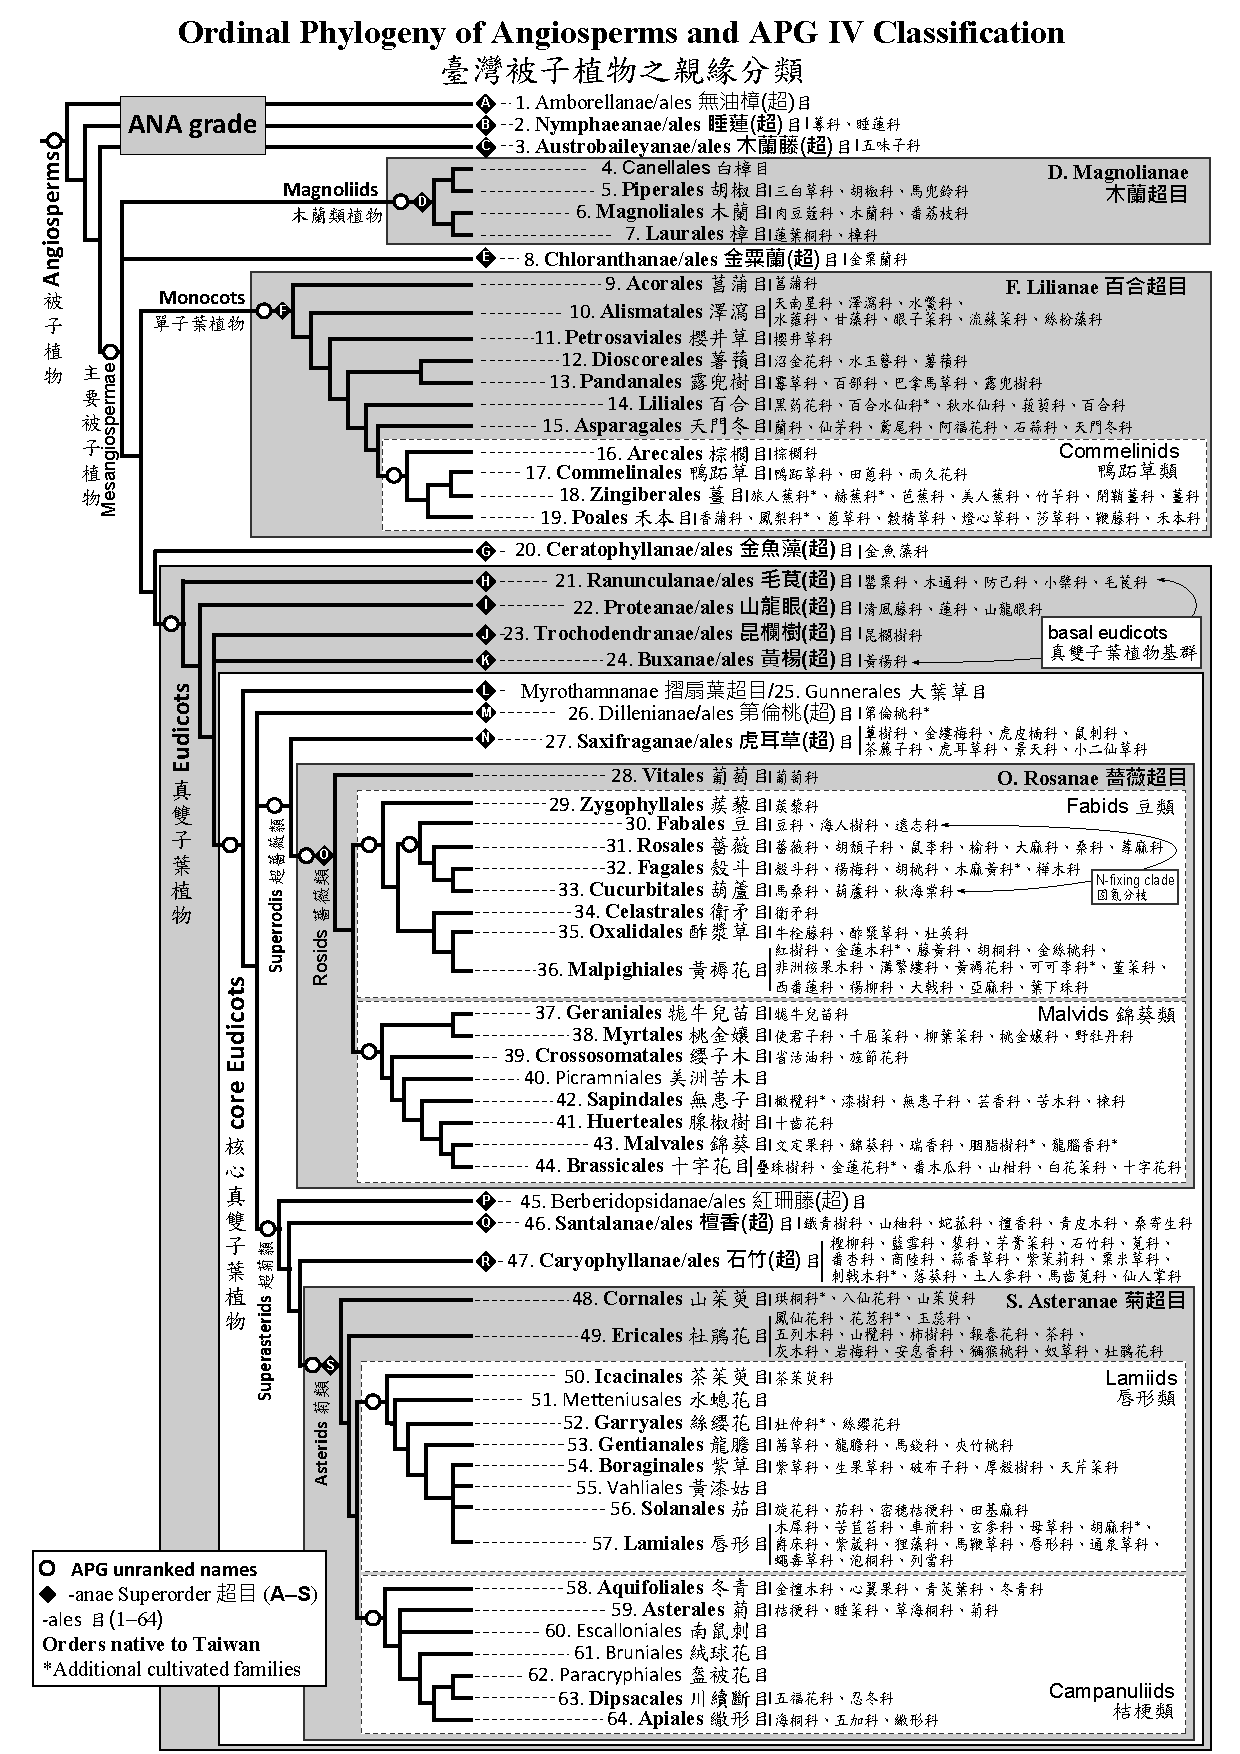
\includepdf{APGIV.pdf}

        \chapter{評估流程}
\begin{multicols}{2}

本報告採用的評估準則(criteria) 與類別 (categories) 係依據 IUCN 紅皮書名錄類別與標 準: 3.1 版 (IUCN 2012b)及 IUCN 紅皮書名錄地區 及國家級評估標準應用指南: 4.0 版(IUCN 2012a) ,並參照 IUCN 紅皮書名錄類別與標準 應用指南 (IUCN Standards and Pe  ons Subcom- mi ee 2017),考慮了原生或外來種的問題,對 臺灣維管束植物進行紅皮書評估。其評估流程 與方法簡述如下:
\end{multicols}
\section{界定納入評估之分類群}
\begin{multicols}{2}
本報告評估的範圍為臺灣本島及附屬島嶼 (彭佳嶼、棉花嶼、花瓶嶼、基隆嶼、澎湖群 島、小琉球、龜山島、綠島、蘭嶼及小蘭嶼) 的野外自生維管束植物物種,但不包括鄰近中 國大陸的金門和馬祖以及東沙和南沙群島。評 估的分類單元原則為「種」,但範圍內同時有 亞種或變種出現時則分別評估,原則上不包括 變種以下階級、雜交種以及外來種。
以「臺灣維管束植物紅皮書初評名錄」(王 震哲等,2012)評估基礎所收集的物種為基 礎,加上新種、新紀錄種以及初評時遺漏的維 管束植物名錄,共有 種自生維管束植物列入 候選評估名單。其次依據 IUCN 紅皮書名錄地 區及國家級評估標準應用指南 (IUCN 2012a) 的 建議流程,排除不適用(Not Applicable)於區域 評估的物種,其餘出現於臺灣本島及附屬島嶼 涵蓋範圍內之維管束植物均列入正式評估清 單,共 種進入評估流程。
\end{multicols}
\section{資訊收集與初步評估}
\begin{multicols}{2}
完成候選評估名單收集後,由編輯委員會
送請相關的專家進行評估。依據 IUCN 紅皮書 名錄類別與標準: 3.1 版(IUCN 2012b) 與 IUCN 地 區及國家級評估標準應用指南: 4.0 版(IUCN 2012a),建立評估資料表,並進行上述列入評 估名單物種的各項資料蒐集。
每一受評分類群均依照 IUCN 紅皮書名錄 類別與標準使用指南: 13 版進行評估(IUCN Standards and Pe  ons Subcommi ee 2017), 得出初步類別 。評估流程係由包括: A. 快速 族群下降(Rapid popula on reduc on)、B. 分布
侷限、碎裂化,同時存在族群下降或嚴重波動
(Small range and fragmented, declining, or ex- treme  uctua ons)、C. 小族群且持續下降 (Small popula on and declining)、D. 非常小的 族群(Very small popula on),以及 E. 量化分析 (Quan ta ve analysis) 等五大標準及對應之次 要標準(Sub-criterion) 及資格限制(Quali ers)所 構成之決策樹(logic tree) 進行( 表 1)。每個分 類單元都會依所有標準進行評估,只要符合任 一條標準者,即列入受脅物種的類別,並在文 件報告中列出符合類別的標準及對應之次標 準。至於若無法符合極危、瀕危及易危的類 別,但已很接近或未來可能達到易危類別時, 則列入接近受脅(Near-threatened, NT) 類別。 某一物種經過評估後,無法符合國家極危 (Na onally Cri cally Endangered, NCR)、國家瀕 危(Na onally Endangered, NEN) 及國家易危 (Na onally Vulnerable, NVU) 的類別,但已很接 近或未來可能達到國家易危類別時,可列入國 家接近受脅(Na onally Near-threatened, NNT)。 由於 IUCN 紅皮書名錄類別與標準並無明確的 接近受脅(NT) 標準定義,本報告根據前述原則 設定本報告國家接近受脅的標準(表 1)。
\end{multicols}
\includepdf{iucn_standards.pdf}
\includepdf{iucn_standards2.pdf}

\section{類別調整}
\begin{multicols}{2}
依據資料完成各分類群的初步類別評估 後,若果該分類群非台灣特有,需進一步考慮 受評估分類群的區域滅絕機率受到評估範圍外 相同分類群其他族群的影響程度(IUCN
2012a) ,並依據評估結果將該分類群的初步類 別予以升級、降級或維持不變。
調整類別的原則依照 IUCN(2012a) 建議流 程,針對臺灣族群區域標準,說明如下:


\end{multicols}

\fbox{
    \begin{minipage}{0.9\textwidth}
\begin{enumerate}
    \item[1.] 若該分類群為台灣特有,維持步驟 2.2 之評估類別結果。 \\
    \item[2.] 若該分類群非台灣特有,則再依下列原則進行評估,並依據評估結果將該分類群的類別予以升級、降級或維持不變:\\
    \begin{enumerate}
        \item[(1)] 如果原分布地區或台灣地區的棲息地環境有惡化現象,其類別保持不變。\\
        \item[(2) ] 如果在相鄰地區沒有同種族群或其繁殖體不能播遷到台灣,台灣族群可以視為本地特有的,其 類別保持不變。\\
        \item[(3) ] 如果區外族群個體不可能在台灣存活,類別保持不變。 \\
        \item[(4) ] 如果沒有足夠的適宜棲息地或是現有保護措施不能在可預見的將來改善棲息地環境,區外的移入將不會降低絕滅危險,類別保持不變。\\
        \item[(5) ] 如果分類群在區外相對比較普遍,沒有族群衰退的跡象,且能夠播遷並有(或即將有)可利用的潛在棲息地,則降低其等級。如果分類群在相鄰地區正在減少,“救助影響”不容易發生,則 提高類別。\\

        \item[(6) ] 如果有跡象表明一定數量的繁殖體定期到達該地而族群仍然只有少量存活,則地區族群可能爲 “數量衰減”。若是如此,繁殖體移入有即將停止的趨勢,提高類別。 \\
    \end{enumerate}
\end{enumerate}
\end{minipage}
}


\section{公開意見徵詢}
\begin{multicols}{2}
經由步驟 2.1 至 2.3 產生的評估結果,於 2017 年 6 月至 11 月徵求並彙整台灣植物分類 學會全體會員及全國相關機關(如林試所、中研 院生物多樣性中心、自然科學博物館...等)、團 體及個人對於評定類別是否有所不當而需修改
之意見,並於 2017 年 12 月 1 日與林務局共同 召開「臺灣維管束植物紅皮書成果說明會」, 廣泛徵求意見,最後再依據更新之資訊,再次 執行 2.1 至 2.3 步驟後產生本報告。

\end{multicols}

    \end{Kai}
    \chapter{臺灣維管束植物評估結果}


\section{滅絕(EX)、野外滅絕(EW)與區域滅絕(RE)物種}
\section{極度瀕危(CR)物種名錄}
\section{瀕危(EN)物種名錄}
\section{易危(VU)物種名錄}
\section{接近受脅(NT)物種名錄}
\section{資料缺乏(DD)物種名錄}
\section{暫無危機(LC)物種名錄}
\section{不適用(NA)物種名錄}
\section{排除評估物種名錄與說明}

\section{評估結果總名錄}
\begin{multicols}{2}
\noindent \normalsize\textsc{\textbf{ANA grade} 被子植物ANA基群}\selectfont \\
\footnotesize\selectfont
\begin{enumerate}
  \item[2. ] \textbf{\textsc{Nymphaeales} 睡蓮目} 
    \begin{enumerate}
      \item[2.3] Cabombaceae 蓴科(蓴菜科)  
        
  \begin{itemize}
 \item[] \textit{Brasenia} 蓴屬
                    
  \begin{itemize}
        \item[] \href{http://www.theplantlist.org/tpl1.1/search?q=Brasenia+schreberi}{\textit{B. schreberi} J.F.Gmel.}  \index{Brasenia@\textit{Brasenia}!schreberi@\textbf{\textit{schreberi}}} \href{\detokenize{http://taibnet.sinica.edu.tw/chi/taibnet_species_list.php?T2=蓴&T2_new_value=true&fr=y}}{蓴}\index{蓴@{\Song{蓴}}} VU
  \end{itemize}
 \item[] \textit{Cabomba} 穗蓴屬
                    
  \begin{itemize}
        \item[] \href{http://www.theplantlist.org/tpl1.1/search?q=Cabomba+caroliniana}{\textit{C. caroliniana} A.Gray}  \index{Cabomba@\textit{Cabomba}!caroliniana@\textit{caroliniana}} \href{\detokenize{http://taibnet.sinica.edu.tw/chi/taibnet_species_list.php?T2=白花穗蓴&T2_new_value=true&fr=y}}{白花穗蓴}\index{白花穗蓴} NA$^n$
        \item[] \href{http://www.theplantlist.org/tpl1.1/search?q=Cabomba+furcata}{\textit{C. furcata} Schult. \& Schult.f.}  \index{Cabomba@\textit{Cabomba}!furcata@\textit{furcata}} \href{\detokenize{http://taibnet.sinica.edu.tw/chi/taibnet_species_list.php?T2=紅花穗蓴&T2_new_value=true&fr=y}}{紅花穗蓴}\index{紅花穗蓴} NA$^n$
  \end{itemize}
  \end{itemize}

      \item[2.4] Nymphaeaceae 睡蓮科  
        
  \begin{itemize}
 \item[] \textit{Euryale} 芡屬
                                
  \begin{itemize}
        \item[] \textit{E. ferox} Salisb. \index{Euryale@\textit{Euryale}!ferox@\textit{ferox}} 芡 \index{芡}  CR
  \end{itemize}
 \item[] \textit{Nuphar} 萍蓬草屬
                                
  \begin{itemize}
        \item[] \textit{N. shimadai} Hayata \index{Nuphar@\textit{Nuphar}!shimadai@\textit{shimadai}} 臺灣萍蓬草 \index{臺灣萍蓬草} \# CR
  \end{itemize}
 \item[] \textit{Nymphaea} 睡蓮屬
                                
  \begin{itemize}
        \item[] \textit{N. nouchali} Burm.f. \index{Nymphaea@\textit{Nymphaea}!nouchali@\textit{nouchali}} 白花睡蓮 \index{白花睡蓮}  DD
        \item[] \textit{N. stellata} Willd. \index{Nymphaea@\textit{Nymphaea}!stellata@\textit{stellata}} 藍睡蓮 \index{藍睡蓮}  DD
        \item[] \textit{N. tetragona} Georgi \index{Nymphaea@\textit{Nymphaea}!tetragona@\textit{tetragona}} 睡蓮 \index{睡蓮}  DD
  \end{itemize}
  \end{itemize}

    \end{enumerate}
  \item[3. ] \textbf{\textsc{Austrobaileyales} 木蘭藤目} 
    \begin{enumerate}
      \item[3.7] Schisandraceae 五味子科  
        
  \begin{itemize}
 \item[] \textit{Illicium}\index{Illicium@\textit{Illicium}} 八角屬
                                
  \begin{itemize}
        \item[] \textit{I. anisatum} L. \index{Illicium@\textit{Illicium}!anisatum@\textit{anisatum}} 白花八角 \index{白花八角}  LC
        \item[] \textit{I. arborescens} Hayata \index{Illicium@\textit{Illicium}!arborescens@\textit{arborescens}} 臺灣八角 \index{臺灣八角} \# LC
        \item[] \textit{I. tashiroi} Maxim. \index{Illicium@\textit{Illicium}!tashiroi@\textit{tashiroi}} 東亞八角 \index{東亞八角}  LC
  \end{itemize}
 \item[] \textit{Kadsura}\index{Kadsura@\textit{Kadsura}} 南五味子屬
                                
  \begin{itemize}
        \item[] \textit{K. japonica} (L.) Dunal \index{Kadsura@\textit{Kadsura}!japonica@\textit{japonica}} 南五味子 \index{南五味子}  LC
        \item[] \textit{K. philippinensis} Elmer \index{Kadsura@\textit{Kadsura}!philippinensis@\textit{philippinensis}} 菲律賓五味子 \index{菲律賓五味子}  NT
  \end{itemize}
 \item[] \textit{Schisandra}\index{Schisandra@\textit{Schisandra}} 五味子屬
                                
  \begin{itemize}
        \item[] \textit{S. arisanensis} Hayata \index{Schisandra@\textit{Schisandra}!arisanensis@\textit{arisanensis}} 阿里山五味子 \index{阿里山五味子} \# LC
  \end{itemize}
  \end{itemize}

    \end{enumerate}
\end{enumerate}
\vspace{2ex} 
\noindent \normalsize\textsc{\textbf{Independent lineage} 獨立支序}\selectfont \\
\footnotesize\selectfont
\begin{enumerate}
  \item[8. ] \textbf{\textsc{Chloranthales} 金粟蘭目} 
    \begin{enumerate}
      \item[8.26] Chloranthaceae 金粟蘭科  
        
  \begin{itemize}
 \item[] \textit{Chloranthus}\index{Chloranthus@\textit{Chloranthus}} 金粟蘭屬
                                
  \begin{itemize}
        \item[] \textit{C. henryi} Hemsl. \index{Chloranthus@\textit{Chloranthus}!henryi@\textit{henryi}} 寬葉金粟蘭 \index{寬葉金粟蘭}  LC
        \item[] \textit{C. oldhami} Solms. \index{Chloranthus@\textit{Chloranthus}!oldhami@\textit{oldhami}} 臺灣及己 \index{臺灣及己}  LC
  \end{itemize}
 \item[] \textit{Sarcandra}\index{Sarcandra@\textit{Sarcandra}} 接骨木屬
                                
  \begin{itemize}
        \item[] \textit{S. glabra} (Thunb.) Nakai \index{Sarcandra@\textit{Sarcandra}!glabra@\textit{glabra}} 草珊瑚 \index{草珊瑚}  LC
  \end{itemize}
  \end{itemize}

    \end{enumerate}
\end{enumerate}
\vspace{2ex} 
\noindent \normalsize\textsc{\textbf{Magnoliids} 木蘭類植物}\selectfont \\
\footnotesize\selectfont
\begin{enumerate}
  \item[5. ] \textbf{\textsc{Piperales} 胡椒目} 
    \begin{enumerate}
      \item[5.10] Saururaceae 三白草科  
        
  \begin{itemize}
 \item[] \textit{Houttuynia} 蕺菜屬
                    
  \begin{itemize}
        \item[] \href{http://www.theplantlist.org/tpl1.1/search?q=Houttuynia+cordata}{\textit{H. cordata} Thunb.}  \index{Houttuynia@\textit{Houttuynia}!cordata@\textit{cordata}} \href{\detokenize{http://taibnet.sinica.edu.tw/chi/taibnet_species_list.php?T2=臭腥草&T2_new_value=true&fr=y}}{臭腥草}\index{臭腥草} LC
  \end{itemize}
 \item[] \textit{Saururus} 三白草屬
                    
  \begin{itemize}
        \item[] \href{http://www.theplantlist.org/tpl1.1/search?q=Saururus+chinensis}{\textit{S. chinensis} (Lour.) Baill.}  \index{Saururus@\textit{Saururus}!chinensis@\textit{chinensis}} \href{\detokenize{http://taibnet.sinica.edu.tw/chi/taibnet_species_list.php?T2=三白草&T2_new_value=true&fr=y}}{三白草}\index{三白草} LC
  \end{itemize}
  \end{itemize}

      \item[5.11] Piperaceae 胡椒科  
        
  \begin{itemize}
 \item[] \textit{Peperomia}\index{Peperomia@\textit{Peperomia}} 椒草屬
                                
  \begin{itemize}
        \item[] \textit{P. japonica} Makino \index{Peperomia@\textit{Peperomia}!japonica@\textit{japonica}} 椒草 \index{椒草}  LC
        \item[] \textit{P. nakaharai} Hayata \index{Peperomia@\textit{Peperomia}!nakaharai@\textit{nakaharai}} 山椒草 \index{山椒草} \# LC
        \item[] \textit{P. pellucida} Kunth \index{Peperomia@\textit{Peperomia}!pellucida@\textit{pellucida}} 草胡椒 \index{草胡椒}  NA
        \item[] \textit{P. reflexa} (L. f.) A. Dietr. \index{Peperomia@\textit{Peperomia}!reflexa@\textit{reflexa}} 小椒草 \index{小椒草}  LC
        \item[] \textit{P. rubrivenosa} C. DC. \index{Peperomia@\textit{Peperomia}!rubrivenosa@\textit{rubrivenosa}} 蘭嶼椒草 \index{蘭嶼椒草}  LC
        \item[] \textit{P. sui} T. T. Lin \& S. Y. Lu \index{Peperomia@\textit{Peperomia}!sui@\textit{sui}} 紅莖椒草 \index{紅莖椒草} \# LC
  \end{itemize}
 \item[] \textit{Piper}\index{Piper@\textit{Piper}} 胡椒屬
                                
  \begin{itemize}
        \item[] \textit{P. arborescens} Roxb. \index{Piper@\textit{Piper}!arborescens@\textit{arborescens}} 蘭嶼風藤 \index{蘭嶼風藤}  LC
        \item[] \textit{P. betle} L. \index{Piper@\textit{Piper}!betle@\textit{betle}} 荖藤 \index{荖藤}  NA
        \item[] \textit{P. interruptum} var. \textit{multinervum} C. DC. \index{Piper@\textit{Piper}!interruptum@\textit{interruptum}!var. multinervum@var. \textit{multinervum}} 多脈風藤 \index{多脈風藤}  DD
        \item[] \textit{P. kadsura} (Choisy) Ohwi \index{Piper@\textit{Piper}!kadsura@\textit{kadsura}} 風藤 \index{風藤}  LC
        \item[] \textit{P. kawakamii} Hayata \index{Piper@\textit{Piper}!kawakamii@\textit{kawakamii}} 恆春風藤 \index{恆春風藤} \# LC
        \item[] \textit{P. kwashoense} Hayata \index{Piper@\textit{Piper}!kwashoense@\textit{kwashoense}} 綠島風藤 \index{綠島風藤} \# LC
        \item[] \textit{P. sarmentosum} Roxb. \index{Piper@\textit{Piper}!sarmentosum@\textit{sarmentosum}} 假蒟 \index{假蒟}  NA
        \item[] \textit{P. sintenense} Hatus. \index{Piper@\textit{Piper}!sintenense@\textit{sintenense}} 薄葉風藤 \index{薄葉風藤} \# LC
        \item[] \textit{P. taiwanense} T. T. Lin \& S. Y. Lu \index{Piper@\textit{Piper}!taiwanense@\textit{taiwanense}} 臺灣荖藤 \index{臺灣荖藤} \# LC
        \item[] \textit{P. umbellatum} L. \index{Piper@\textit{Piper}!umbellatum@\textit{umbellatum}} 臺灣胡椒 \index{臺灣胡椒}  LC
  \end{itemize}
  \end{itemize}

      \item[5.12] Aristolochiaceae 馬兜鈴科  
        
  \begin{itemize}
 \item[] \textit{Aristolochia} 馬兜鈴屬
                    
  \begin{itemize}
        \item[] \href{http://www.theplantlist.org/tpl1.1/search?q=Aristolochia+cucurbitifolia}{\textit{A. cucurbitifolia} Hayata}  \index{Aristolochia@\textit{Aristolochia}!cucurbitifolia@\textbf{\textit{cucurbitifolia}}} \href{\detokenize{http://taibnet.sinica.edu.tw/chi/taibnet_species_list.php?T2=瓜葉馬兜鈴&T2_new_value=true&fr=y}}{瓜葉馬兜鈴}\index{瓜葉馬兜鈴@{\Song{瓜葉馬兜鈴}}}\# VU
        \item[] \href{http://www.theplantlist.org/tpl1.1/search?q=Aristolochia+foveolata}{\textit{A. foveolata} Merr.}  \index{Aristolochia@\textit{Aristolochia}!foveolata@\textit{foveolata}} \href{\detokenize{http://taibnet.sinica.edu.tw/chi/taibnet_species_list.php?T2=蜂窩馬兜鈴&T2_new_value=true&fr=y}}{蜂窩馬兜鈴}\index{蜂窩馬兜鈴} NT
        \item[] \href{http://www.theplantlist.org/tpl1.1/search?q=Aristolochia+heterophylla}{\textit{A. heterophylla} Hemsl.}  \index{Aristolochia@\textit{Aristolochia}!heterophylla@\textit{heterophylla}} \href{\detokenize{http://taibnet.sinica.edu.tw/chi/taibnet_species_list.php?T2=異葉馬兜鈴&T2_new_value=true&fr=y}}{異葉馬兜鈴}\index{異葉馬兜鈴} LC
        \item[] \href{http://www.theplantlist.org/tpl1.1/search?q=Aristolochia+yujungiana}{\textit{A. yujungiana} C.T.Lu \& J.C.Wang}  \index{Aristolochia@\textit{Aristolochia}!yujungiana@\textbf{\textit{yujungiana}}} \href{\detokenize{http://taibnet.sinica.edu.tw/chi/taibnet_species_list.php?T2=裕榮馬兜鈴&T2_new_value=true&fr=y}}{裕榮馬兜鈴}\index{裕榮馬兜鈴@{\Song{裕榮馬兜鈴}}}\# CR
        \item[] \href{http://www.theplantlist.org/tpl1.1/search?q=Aristolochia+zollingeriana}{\textit{A. zollingeriana} Miq.}  \index{Aristolochia@\textit{Aristolochia}!zollingeriana@\textit{zollingeriana}} \href{\detokenize{http://taibnet.sinica.edu.tw/chi/taibnet_species_list.php?T2=港口馬兜鈴&T2_new_value=true&fr=y}}{港口馬兜鈴}\index{港口馬兜鈴} NT
  \end{itemize}
 \item[] \textit{Asarum} 細辛屬
                    
  \begin{itemize}
        \item[] \href{http://www.theplantlist.org/tpl1.1/search?q=Asarum+caudigerum}{\textit{A. caudigerum} Hance}  \index{Asarum@\textit{Asarum}!caudigerum@\textit{caudigerum}} \href{\detokenize{http://taibnet.sinica.edu.tw/chi/taibnet_species_list.php?T2=薄葉細辛&T2_new_value=true&fr=y}}{薄葉細辛}\index{薄葉細辛} LC
        \item[] \href{http://www.theplantlist.org/tpl1.1/search?q=Asarum+chatienshanianum}{\textit{A. chatienshanianum} C.T.Lu \& J.C.Wang}  \index{Asarum@\textit{Asarum}!chatienshanianum@\textbf{\textit{chatienshanianum}}} \href{\detokenize{http://taibnet.sinica.edu.tw/chi/taibnet_species_list.php?T2=插天山細辛&T2_new_value=true&fr=y}}{插天山細辛}\index{插天山細辛@{\Song{插天山細辛}}}\# EN
        \item[] \href{http://www.theplantlist.org/tpl1.1/search?q=Asarum+crassusepalum}{\textit{A. crassusepalum} S.F.Huang}  \index{Asarum@\textit{Asarum}!crassusepalum@\textbf{\textit{crassusepalum}}} \href{\detokenize{http://taibnet.sinica.edu.tw/chi/taibnet_species_list.php?T2=鴛鴦湖細辛&T2_new_value=true&fr=y}}{鴛鴦湖細辛}\index{鴛鴦湖細辛@{\Song{鴛鴦湖細辛}}}\# VU
        \item[] \href{http://www.theplantlist.org/tpl1.1/search?q=Asarum+epigynum}{\textit{A. epigynum} Hayata}  \index{Asarum@\textit{Asarum}!epigynum@\textbf{\textit{epigynum}}} \href{\detokenize{http://taibnet.sinica.edu.tw/chi/taibnet_species_list.php?T2=上花細辛&T2_new_value=true&fr=y}}{上花細辛}\index{上花細辛@{\Song{上花細辛}}} VU
        \item[] \href{http://www.theplantlist.org/tpl1.1/search?q=Asarum+hypogynum}{\textit{A. hypogynum} Hayata}  \index{Asarum@\textit{Asarum}!hypogynum@\textbf{\textit{hypogynum}}} \href{\detokenize{http://taibnet.sinica.edu.tw/chi/taibnet_species_list.php?T2=下花細辛&T2_new_value=true&fr=y}}{下花細辛}\index{下花細辛@{\Song{下花細辛}}}\# VU
        \item[] \href{http://www.theplantlist.org/tpl1.1/search?q=Asarum+macranthum}{\textit{A. macranthum} Hook.f.}  \index{Asarum@\textit{Asarum}!macranthum@\textit{macranthum}} \href{\detokenize{http://taibnet.sinica.edu.tw/chi/taibnet_species_list.php?T2=大花細辛&T2_new_value=true&fr=y}}{大花細辛}\index{大花細辛}\# LC
        \item[] \href{http://www.theplantlist.org/tpl1.1/search?q=Asarum+satsumense}{\textit{A. satsumense} F.Maek.}  \index{Asarum@\textit{Asarum}!satsumense@\textbf{\textit{satsumense}}} \href{\detokenize{http://taibnet.sinica.edu.tw/chi/taibnet_species_list.php?T2=薩摩細辛&T2_new_value=true&fr=y}}{薩摩細辛}\index{薩摩細辛@{\Song{薩摩細辛}}} EN
        \item[] \href{http://www.theplantlist.org/tpl1.1/search?q=Asarum+taipingshanianum}{\textit{A. taipingshanianum} S.F.Huang}  \index{Asarum@\textit{Asarum}!taipingshanianum@\textbf{\textit{taipingshanianum}}} \href{\detokenize{http://taibnet.sinica.edu.tw/chi/taibnet_species_list.php?T2=太平山細辛&T2_new_value=true&fr=y}}{太平山細辛}\index{太平山細辛@{\Song{太平山細辛}}}\# VU
        \item[] \href{http://www.theplantlist.org/tpl1.1/search?q=Asarum+tawushanianum}{\textit{A. tawushanianum} C.T.Lu \& J.C.Wang}  \index{Asarum@\textit{Asarum}!tawushanianum@\textbf{\textit{tawushanianum}}} \href{\detokenize{http://taibnet.sinica.edu.tw/chi/taibnet_species_list.php?T2=大武山細辛&T2_new_value=true&fr=y}}{大武山細辛}\index{大武山細辛@{\Song{大武山細辛}}}\# CR
        \item[] \href{http://www.theplantlist.org/tpl1.1/search?q=Asarum+villisepalum}{\textit{A. villisepalum} C.T.Lu \& J.C.Wang}  \index{Asarum@\textit{Asarum}!villisepalum@\textbf{\textit{villisepalum}}} \href{\detokenize{http://taibnet.sinica.edu.tw/chi/taibnet_species_list.php?T2=神秘湖細辛&T2_new_value=true&fr=y}}{神秘湖細辛}\index{神秘湖細辛@{\Song{神秘湖細辛}}}\# EN
        \item[] \href{http://www.theplantlist.org/tpl1.1/search?q=Asarum+yaeyamense}{\textit{A. yaeyamense} Hatusima}  \index{Asarum@\textit{Asarum}!yaeyamense@\textbf{\textit{yaeyamense}}} \href{\detokenize{http://taibnet.sinica.edu.tw/chi/taibnet_species_list.php?T2=八重山細辛&T2_new_value=true&fr=y}}{八重山細辛}\index{八重山細辛@{\Song{八重山細辛}}} EN
  \end{itemize}
  \end{itemize}

    \end{enumerate}
  \item[6. ] \textbf{\textsc{Magnoliales} 木蘭目} 
    \begin{enumerate}
      \item[6.13] Myristicaceae 肉荳蔻科  
        
  \begin{itemize}
 \item[] \textit{Myristica} 肉荳蔻屬
                                
  \begin{itemize}
        \item[] \href{http://www.theplantlist.org/tpl1.1/search?q=Myristica+ceylanica+var.+cagayanensis}{\textit{M. ceylanica} A.DC. var. \textit{cagayanensis} (Merr.) J. Sinclair}  \index{Myristica@\textit{Myristica}!ceylanica@\textit{ceylanica}!var. cagayanensis@var. \textit{cagayanensis}} 蘭嶼肉荳蔻 \index{蘭嶼肉荳蔻}  VU
        \item[] \href{http://www.theplantlist.org/tpl1.1/search?q=Myristica+elliptica+var.+simiarum}{\textit{M. elliptica} Wall. ex Hook.f. \& Thomson var. \textit{simiarum} (A.DC.) J.Sinclair}  \index{Myristica@\textit{Myristica}!elliptica@\textit{elliptica}!var. simiarum@var. \textit{simiarum}} 紅頭肉豆蔻 \index{紅頭肉豆蔻}  EN
  \end{itemize}
  \end{itemize}

      \item[6.14] Magnoliaceae 木蘭科  
        
  \begin{itemize}
 \item[] \textit{Magnolia} 木蘭屬
                                
  \begin{itemize}
        \item[] \href{http://www.theplantlist.org/tpl1.1/search?q=Magnolia+kachirachirai}{\textit{M. kachirachirai} (Kaneh. \& Yamam.) Dandy}  \index{Magnolia@\textit{Magnolia}!kachirachirai@\textit{kachirachirai}} 烏心石舅 \index{烏心石舅} \# VU
  \end{itemize}
 \item[] \textit{Michelia} 烏心石屬
                                
  \begin{itemize}
        \item[] \href{http://www.theplantlist.org/tpl1.1/search?q=Michelia+compressa+var.+formosana}{\textit{M. compressa} (Maxim.) Sargent var. \textit{formosana} Kanah.}  \index{Michelia@\textit{Michelia}!compressa@\textit{compressa}!var. formosana@var. \textit{formosana}} 臺灣烏心石 \index{臺灣烏心石} \# LC
        \item[] \href{http://www.theplantlist.org/tpl1.1/search?q=Michelia+compressa+var.+lanyuensis}{\textit{M. compressa} (Maxim.) Sargent var. \textit{lanyuensis} S.Y.Lu}  \index{Michelia@\textit{Michelia}!compressa@\textit{compressa}!var. lanyuensis@var. \textit{lanyuensis}} 蘭嶼烏心石 \index{蘭嶼烏心石} \# LC
  \end{itemize}
  \end{itemize}

      \item[6.18] Annonaceae 番荔枝科  
        
  \begin{itemize}
 \item[] \textit{Fissistigma} 瓜馥木屬
                    
  \begin{itemize}
        \item[] \href{http://www.theplantlist.org/tpl1.1/search?q=Fissistigma+glaucescens}{\textit{F. glaucescens} (Hance) Merr.}  \index{Fissistigma@\textit{Fissistigma}!glaucescens@\textit{glaucescens}} \href{\detokenize{http://taibnet.sinica.edu.tw/chi/taibnet_species_list.php?T2=裏白瓜馥木&T2_new_value=true&fr=y}}{裏白瓜馥木}\index{裏白瓜馥木} DD
        \item[] \href{http://www.theplantlist.org/tpl1.1/search?q=Fissistigma+oldhamii}{\textit{F. oldhamii} (Hemsl.) Merr.}  \index{Fissistigma@\textit{Fissistigma}!oldhamii@\textit{oldhamii}} \href{\detokenize{http://taibnet.sinica.edu.tw/chi/taibnet_species_list.php?T2=瓜馥木&T2_new_value=true&fr=y}}{瓜馥木}\index{瓜馥木} LC
  \end{itemize}
 \item[] \textit{Goniothalamus} 哥納香屬
                    
  \begin{itemize}
        \item[] \href{http://www.theplantlist.org/tpl1.1/search?q=Goniothalamus+amuyon}{\textit{G. amuyon} (Blanco) Merr.}  \index{Goniothalamus@\textit{Goniothalamus}!amuyon@\textbf{\textit{amuyon}}} \href{\detokenize{http://taibnet.sinica.edu.tw/chi/taibnet_species_list.php?T2=恆春哥納香&T2_new_value=true&fr=y}}{恆春哥納香}\index{恆春哥納香@{\Song{恆春哥納香}}} CR
  \end{itemize}
 \item[] \textit{Polyalthia} 暗羅屬
                    
  \begin{itemize}
        \item[] \href{http://www.theplantlist.org/tpl1.1/search?q=Polyalthia+liukiuensis}{\textit{P. liukiuensis} Hatus.}  \index{Polyalthia@\textit{Polyalthia}!liukiuensis@\textbf{\textit{liukiuensis}}} \href{\detokenize{http://taibnet.sinica.edu.tw/chi/taibnet_species_list.php?T2=琉球暗羅&T2_new_value=true&fr=y}}{琉球暗羅}\index{琉球暗羅@{\Song{琉球暗羅}}} CR
  \end{itemize}
  \end{itemize}

    \end{enumerate}
  \item[7. ] \textbf{\textsc{Laurales} 樟目} 
    \begin{enumerate}
      \item[7.23] Hernandiaceae 蓮葉桐科  
        
  \begin{itemize}
 \item[] \textit{Hernandia} 蓮葉桐屬
                    
  \begin{itemize}
        \item[] \href{http://www.theplantlist.org/tpl1.1/search?q=Hernandia+nymphiifolia}{\textit{H. nymphiifolia} (C.Presl) Kubitzki}  \index{Hernandia@\textit{Hernandia}!nymphiifolia@\textit{nymphiifolia}} 蓮葉桐\index{蓮葉桐} VU
  \end{itemize}
 \item[] \textit{Illigera} 青藤屬
                    
  \begin{itemize}
        \item[] \href{http://www.theplantlist.org/tpl1.1/search?q=Illigera+luzonensis}{\textit{I. luzonensis} (C.Presl) Merr.}  \index{Illigera@\textit{Illigera}!luzonensis@\textit{luzonensis}} 呂宋青藤\index{呂宋青藤} LC
  \end{itemize}
  \end{itemize}

      \item[7.25] Lauraceae 樟科  
        
  \begin{itemize}
 \item[] \textit{Beilschmiedia} 瓊楠屬
                                
  \begin{itemize}
        \item[] \href{http://www.theplantlist.org/tpl1.1/search?q=Beilschmiedia+erythrophloia}{\textit{B. erythrophloia} Hayata}  \index{Beilschmiedia@\textit{Beilschmiedia}!erythrophloia@\textit{erythrophloia}} 瓊楠 \index{瓊楠}  LC
        \item[] \href{http://www.theplantlist.org/tpl1.1/search?q=Beilschmiedia+tsangii}{\textit{B. tsangii} Merr.}  \index{Beilschmiedia@\textit{Beilschmiedia}!tsangii@\textit{tsangii}} 華河瓊楠 \index{華河瓊楠}  LC
  \end{itemize}
 \item[] \textit{Cassytha} 無根草屬
                                
  \begin{itemize}
        \item[] \href{http://www.theplantlist.org/tpl1.1/search?q=Cassytha+filiformis}{\textit{C. filiformis} L.}  \index{Cassytha@\textit{Cassytha}!filiformis@\textit{filiformis}} 無根草 \index{無根草}  LC
  \end{itemize}
 \item[] \textit{Cinnamomum} 樟屬
                                
  \begin{itemize}
        \item[] \href{http://www.theplantlist.org/tpl1.1/search?q=Cinnamomum+austrosinense}{\textit{C. austrosinense} H.T.Chang}  \index{Cinnamomum@\textit{Cinnamomum}!austrosinense@\textit{austrosinense}} 牡丹葉桂皮 \index{牡丹葉桂皮}  EN
        \item[] \href{http://www.theplantlist.org/tpl1.1/search?q=Cinnamomum+brevipedunculatum}{\textit{C. brevipedunculatum} C.E.Chang}  \index{Cinnamomum@\textit{Cinnamomum}!brevipedunculatum@\textit{brevipedunculatum}} 小葉樟 \index{小葉樟} \# VU
        \item[] \href{http://www.theplantlist.org/tpl1.1/search?q=Cinnamomum+burmannii}{\textit{C. burmannii} (Nees) Blume}  \index{Cinnamomum@\textit{Cinnamomum}!burmannii@\textit{burmannii}} 陰香 \index{陰香}  NA (N)
        \item[] \href{http://www.theplantlist.org/tpl1.1/search?q=Cinnamomum+camphora+var.+camphora}{\textit{C. camphora} (L.) J.Presl. var. \textit{camphora}}  \index{Cinnamomum@\textit{Cinnamomum}!camphora@\textit{camphora}!var. camphora@var. \textit{camphora}} 樟樹 \index{樟樹}  LC
        \item[] \href{http://www.theplantlist.org/tpl1.1/search?q=Cinnamomum+camphora+var.+nominale}{\textit{C. camphora} (L.) J.Presl. var. \textit{nominale} Hayata ex Matsum. \& Hayata}  \index{Cinnamomum@\textit{Cinnamomum}!camphora@\textit{camphora}!var. nominale@var. \textit{nominale}} 栳樟 \index{栳樟} \# LC
        \item[] \href{http://www.theplantlist.org/tpl1.1/search?q=Cinnamomum+insulari-montanum}{\textit{C. insulari-montanum} Hayata}  \index{Cinnamomum@\textit{Cinnamomum}!insulari-montanum@\textit{insulari-montanum}} 臺灣肉桂 \index{臺灣肉桂} \# LC
        \item[] \href{http://www.theplantlist.org/tpl1.1/search?q=Cinnamomum+kanehirae}{\textit{C. kanehirae} Hayata}  \index{Cinnamomum@\textit{Cinnamomum}!kanehirae@\textit{kanehirae}} 牛樟 \index{牛樟} \# EN
        \item[] \href{http://www.theplantlist.org/tpl1.1/search?q=Cinnamomum+kotoense}{\textit{C. kotoense} Kaneh. \& Sasaki}  \index{Cinnamomum@\textit{Cinnamomum}!kotoense@\textit{kotoense}} 蘭嶼肉桂 \index{蘭嶼肉桂} \# CR
        \item[] \href{http://www.theplantlist.org/tpl1.1/search?q=Cinnamomum+macrostemon}{\textit{C. macrostemon} Hayata}  \index{Cinnamomum@\textit{Cinnamomum}!macrostemon@\textit{macrostemon}} 胡氏肉桂 \index{胡氏肉桂} \# DD
        \item[] \href{http://www.theplantlist.org/tpl1.1/search?q=Cinnamomum+micranthum}{\textit{C. micranthum} (Hayata) Hayata}  \index{Cinnamomum@\textit{Cinnamomum}!micranthum@\textit{micranthum}} 冇樟 \index{冇樟}  LC
        \item[] \href{http://www.theplantlist.org/tpl1.1/search?q=Cinnamomum+osmophloeum}{\textit{C. osmophloeum} Kaneh.}  \index{Cinnamomum@\textit{Cinnamomum}!osmophloeum@\textit{osmophloeum}} 土肉桂 \index{土肉桂} \# NT
        \item[] \href{http://www.theplantlist.org/tpl1.1/search?q=Cinnamomum+reticulatum}{\textit{C. reticulatum} Hayata}  \index{Cinnamomum@\textit{Cinnamomum}!reticulatum@\textit{reticulatum}} 土樟 \index{土樟} \# NT
        \item[] \href{http://www.theplantlist.org/tpl1.1/search?q=Cinnamomum+subavenium}{\textit{C. subavenium} Miq.}  \index{Cinnamomum@\textit{Cinnamomum}!subavenium@\textit{subavenium}} 香桂 \index{香桂}  LC
        \item[] \href{http://www.theplantlist.org/tpl1.1/search?q=Cinnamomum+tenuifolium}{\textit{C. tenuifolium} (Makino) Sugim.}  \index{Cinnamomum@\textit{Cinnamomum}!tenuifolium@\textit{tenuifolium}} 天竺桂 \index{天竺桂}  
  \end{itemize}
 \item[] \textit{Cryptocarya} 厚殼桂屬
                                
  \begin{itemize}
        \item[] \href{http://www.theplantlist.org/tpl1.1/search?q=Cryptocarya+chinensis}{\textit{C. chinensis} (Hance) Hemsl.}  \index{Cryptocarya@\textit{Cryptocarya}!chinensis@\textit{chinensis}} 厚殼桂 \index{厚殼桂}  LC
        \item[] \href{http://www.theplantlist.org/tpl1.1/search?q=Cryptocarya+concinna}{\textit{C. concinna} Hance}  \index{Cryptocarya@\textit{Cryptocarya}!concinna@\textit{concinna}} 土楠 \index{土楠}  LC
        \item[] \href{http://www.theplantlist.org/tpl1.1/search?q=Cryptocarya+elliptifolia}{\textit{C. elliptifolia} Merr.}  \index{Cryptocarya@\textit{Cryptocarya}!elliptifolia@\textit{elliptifolia}} 菲律賓厚殼桂 \index{菲律賓厚殼桂}  CR
  \end{itemize}
 \item[] \textit{Dehaasia} 腰果楠屬
                                
  \begin{itemize}
        \item[] \href{http://www.theplantlist.org/tpl1.1/search?q=Dehaasia+incrassata}{\textit{D. incrassata} (Jack.) Kosterm.}  \index{Dehaasia@\textit{Dehaasia}!incrassata@\textit{incrassata}} 腰果楠 \index{腰果楠}  CR
  \end{itemize}
 \item[] \textit{Endiandra} 三蕊楠屬
                                
  \begin{itemize}
        \item[] \href{http://www.theplantlist.org/tpl1.1/search?q=Endiandra+coriacea}{\textit{E. coriacea} Merr.}  \index{Endiandra@\textit{Endiandra}!coriacea@\textit{coriacea}} 三蕊楠 \index{三蕊楠}  CR
  \end{itemize}
 \item[] \textit{Lindera} 釣樟屬
                                
  \begin{itemize}
        \item[] \href{http://www.theplantlist.org/tpl1.1/search?q=Lindera+aggregata}{\textit{L. aggregata} (Sims) Kosterm.}  \index{Lindera@\textit{Lindera}!aggregata@\textit{aggregata}} 天臺烏藥 \index{天臺烏藥}  LC
        \item[] \href{http://www.theplantlist.org/tpl1.1/search?q=Lindera+aggregata}{\textit{L. aggregata} (Sims) Kosterm. fo. \textit{playfairii} (Hemsl.) J.C.Liao}  \index{Lindera@\textit{Lindera}!aggregata@\textit{aggregata}} 小葉烏藥 \index{小葉烏藥}  NA (F)
        \item[] \href{http://www.theplantlist.org/tpl1.1/search?q=Lindera+akoensis}{\textit{L. akoensis} Hayata}  \index{Lindera@\textit{Lindera}!akoensis@\textit{akoensis}} 內苳子 \index{內苳子} \# LC
        \item[] \href{http://www.theplantlist.org/tpl1.1/search?q=Lindera+communis}{\textit{L. communis} Hemsl.}  \index{Lindera@\textit{Lindera}!communis@\textit{communis}} 香葉樹 \index{香葉樹}  LC
        \item[] \href{http://www.theplantlist.org/tpl1.1/search?q=Lindera+erythrocarpa}{\textit{L. erythrocarpa} Makino}  \index{Lindera@\textit{Lindera}!erythrocarpa@\textit{erythrocarpa}} 鐵釘樹 \index{鐵釘樹}  LC
        \item[] \href{http://www.theplantlist.org/tpl1.1/search?q=Lindera+glauca}{\textit{L. glauca} (Siebold \& Zucc.) Blume}  \index{Lindera@\textit{Lindera}!glauca@\textit{glauca}} 白葉釣樟 \index{白葉釣樟}  DD
        \item[] \href{http://www.theplantlist.org/tpl1.1/search?q=Lindera+megaphylla}{\textit{L. megaphylla} Hemsl.}  \index{Lindera@\textit{Lindera}!megaphylla@\textit{megaphylla}} 大香葉樹 \index{大香葉樹}  LC
        \item[] \href{http://www.theplantlist.org/tpl1.1/search?q=Lindera+thunbergii}{\textit{L. thunbergii} (Sieb. \& Zucc.) Makino}  \index{Lindera@\textit{Lindera}!thunbergii@\textit{thunbergii}} 脈葉釣樟 \index{脈葉釣樟}  LC
  \end{itemize}
 \item[] \textit{Litsea} 木薑子屬
                                
  \begin{itemize}
        \item[] \href{http://www.theplantlist.org/tpl1.1/search?q=Litsea+acuminata}{\textit{L. acuminata} (Blume) Kurata}  \index{Litsea@\textit{Litsea}!acuminata@\textit{acuminata}} 長葉木薑子 \index{長葉木薑子}  LC
        \item[] \href{http://www.theplantlist.org/tpl1.1/search?q=Litsea+acutivena}{\textit{L. acutivena} Hayata}  \index{Litsea@\textit{Litsea}!acutivena@\textit{acutivena}} 銳脈木薑子 \index{銳脈木薑子}  LC
        \item[] \href{http://www.theplantlist.org/tpl1.1/search?q=Litsea+akoensis+var.+akoensis}{\textit{L. akoensis} Hayata var. \textit{akoensis}}  \index{Litsea@\textit{Litsea}!akoensis@\textit{akoensis}!var. akoensis@var. \textit{akoensis}} 屏東木薑子 \index{屏東木薑子} \# LC
        \item[] \href{http://www.theplantlist.org/tpl1.1/search?q=Litsea+akoensis+var.+chitouchiaoensis}{\textit{L. akoensis} Hayata var. \textit{chitouchiaoensis} J.C.Liao}  \index{Litsea@\textit{Litsea}!akoensis@\textit{akoensis}!var. chitouchiaoensis@var. \textit{chitouchiaoensis}} 竹頭角木薑子 \index{竹頭角木薑子} \# LC
        \item[] \href{http://www.theplantlist.org/tpl1.1/search?q=Litsea+akoensis+var.+sasakii}{\textit{L. akoensis} Hayata var. \textit{sasakii} (Kamik.) J.C.Liao}  \index{Litsea@\textit{Litsea}!akoensis@\textit{akoensis}!var. sasakii@var. \textit{sasakii}} 狹葉木薑子 \index{狹葉木薑子} \# NT
        \item[] \href{http://www.theplantlist.org/tpl1.1/search?q=Litsea+coreana}{\textit{L. coreana} H.Lév.}  \index{Litsea@\textit{Litsea}!coreana@\textit{coreana}} 鹿皮斑木薑子 \index{鹿皮斑木薑子}  LC
        \item[] \href{http://www.theplantlist.org/tpl1.1/search?q=Litsea+cubeba}{\textit{L. cubeba} (Lour.) Per.}  \index{Litsea@\textit{Litsea}!cubeba@\textit{cubeba}} 山胡椒 \index{山胡椒}  LC
        \item[] \href{http://www.theplantlist.org/tpl1.1/search?q=Litsea+elongata+var.+mushaensis}{\textit{L. elongata} (Wall. ex Nees) Benth. \& Hook.f. var. \textit{mushaensis} (Hayata) J.C.Liao}  \index{Litsea@\textit{Litsea}!elongata@\textit{elongata}!var. mushaensis@var. \textit{mushaensis}} 霧社木薑子 \index{霧社木薑子}  LC
        \item[] \href{http://www.theplantlist.org/tpl1.1/search?q=Litsea+garciae}{\textit{L. garciae} Vidal}  \index{Litsea@\textit{Litsea}!garciae@\textit{garciae}} 蘭嶼木薑子 \index{蘭嶼木薑子}  CR
        \item[] \href{http://www.theplantlist.org/tpl1.1/search?q=Litsea+hypophaea}{\textit{L. hypophaea} Hayata}  \index{Litsea@\textit{Litsea}!hypophaea@\textit{hypophaea}} 黃肉樹 \index{黃肉樹} \# LC
        \item[] \href{http://www.theplantlist.org/tpl1.1/search?q=Litsea+lii+var.+lii}{\textit{L. lii} C.E.Chang var. \textit{lii}}  \index{Litsea@\textit{Litsea}!lii@\textit{lii}!var. lii@var. \textit{lii}} 李氏木薑子 \index{李氏木薑子} \# LC
        \item[] \href{http://www.theplantlist.org/tpl1.1/search?q=Litsea+lii+var.+nunkao-tahangensis}{\textit{L. lii} C.E.Chang var. \textit{nunkao-tahangensis} (J.C.Liao) J.C.Liao}  \index{Litsea@\textit{Litsea}!lii@\textit{lii}!var. nunkao-tahangensis@var. \textit{nunkao-tahangensis}} 能漢木薑子 \index{能漢木薑子} \# LC
        \item[] \href{http://www.theplantlist.org/tpl1.1/search?q=Litsea+linii}{\textit{L. linii} Chang}  \index{Litsea@\textit{Litsea}!linii@\textit{linii}} 林氏木薑子 \index{林氏木薑子}  LC
        \item[] \href{http://www.theplantlist.org/tpl1.1/search?q=Litsea+morrisonensis}{\textit{L. morrisonensis} Hayata}  \index{Litsea@\textit{Litsea}!morrisonensis@\textit{morrisonensis}} 玉山木薑子 \index{玉山木薑子} \# LC
        \item[] \href{http://www.theplantlist.org/tpl1.1/search?q=Litsea+perrottetii}{\textit{L. perrottetii} (Blume) Fern-Vill.}  \index{Litsea@\textit{Litsea}!perrottetii@\textit{perrottetii}} 佩羅特木薑子 \index{佩羅特木薑子}  NA (N)
        \item[] \href{http://www.theplantlist.org/tpl1.1/search?q=Litsea+rotundifolia+var.+oblongifolia}{\textit{L. rotundifolia} Hemsl. var. \textit{oblongifolia} (Nees) Allen}  \index{Litsea@\textit{Litsea}!rotundifolia@\textit{rotundifolia}!var. oblongifolia@var. \textit{oblongifolia}} 橢圓葉木薑子 \index{橢圓葉木薑子}  LC
  \end{itemize}
 \item[] \textit{Machilus} 楨楠屬
                                
  \begin{itemize}
        \item[] \href{http://www.theplantlist.org/tpl1.1/search?q=Machilus+japonica+var.+japonica}{\textit{M. japonica} Siebold \& Zucc. var. \textit{japonica}}  \index{Machilus@\textit{Machilus}!japonica@\textit{japonica}!var. japonica@var. \textit{japonica}} 假長葉楠 \index{假長葉楠}  LC
        \item[] \href{http://www.theplantlist.org/tpl1.1/search?q=Machilus+japonica+var.+kusanoi}{\textit{M. japonica} Siebold \& Zucc. var. \textit{kusanoi} (Hayata) J.C.Liao}  \index{Machilus@\textit{Machilus}!japonica@\textit{japonica}!var. kusanoi@var. \textit{kusanoi}} 大葉楠 \index{大葉楠} \# LC
        \item[] \href{http://www.theplantlist.org/tpl1.1/search?q=Machilus+konishii}{\textit{M. konishii} Hayata}  \index{Machilus@\textit{Machilus}!konishii@\textit{konishii}} 小西氏楠 \index{小西氏楠} \# LC
        \item[] \href{http://www.theplantlist.org/tpl1.1/search?q=Machilus+obovatifolia+var.+obovatifolia}{\textit{M. obovatifolia} (Hayata) Kaneh. \& Sasaki var. \textit{obovatifolia}}  \index{Machilus@\textit{Machilus}!obovatifolia@\textit{obovatifolia}!var. obovatifolia@var. \textit{obovatifolia}} 恆春楨楠 \index{恆春楨楠} \# LC
        \item[] \href{http://www.theplantlist.org/tpl1.1/search?q=Machilus+obovatifolia+var.+taiwuensis}{\textit{M. obovatifolia} (Hayata) Kaneh. \& Sasaki var. \textit{taiwuensis} S.Y.Lu \& T.T.Chen}  \index{Machilus@\textit{Machilus}!obovatifolia@\textit{obovatifolia}!var. taiwuensis@var. \textit{taiwuensis}} 大武楨楠 \index{大武楨楠} \# LC
        \item[] \href{http://www.theplantlist.org/tpl1.1/search?q=Machilus+philippinensis}{\textit{M. philippinensis} Merr.}  \index{Machilus@\textit{Machilus}!philippinensis@\textit{philippinensis}} 菲律賓楠 \index{菲律賓楠}  LC
        \item[] \href{http://www.theplantlist.org/tpl1.1/search?q=Machilus+thunbergii}{\textit{M. thunbergii} Siebold \& Zucc.}  \index{Machilus@\textit{Machilus}!thunbergii@\textit{thunbergii}} 豬腳楠 \index{豬腳楠}  LC
        \item[] \href{http://www.theplantlist.org/tpl1.1/search?q=Machilus+zuihoensis+var.+mushaensis}{\textit{M. zuihoensis} Hayata var. \textit{mushaensis} (F.Y.Lu) Y.C.Liu}  \index{Machilus@\textit{Machilus}!zuihoensis@\textit{zuihoensis}!var. mushaensis@var. \textit{mushaensis}} 青葉楠 \index{青葉楠} \# LC
        \item[] \href{http://www.theplantlist.org/tpl1.1/search?q=Machilus+zuihoensis+var.+zuihoensis}{\textit{M. zuihoensis} Hayata var. \textit{zuihoensis}}  \index{Machilus@\textit{Machilus}!zuihoensis@\textit{zuihoensis}!var. zuihoensis@var. \textit{zuihoensis}} 香楠 \index{香楠} \# LC
  \end{itemize}
 \item[] \textit{Neolitsea} 新木薑子屬
                                
  \begin{itemize}
        \item[] \href{http://www.theplantlist.org/tpl1.1/search?q=Neolitsea+aciculata+var.+aciculata}{\textit{N. aciculata} (Blume) Koidz. var. \textit{aciculata}}  \index{Neolitsea@\textit{Neolitsea}!aciculata@\textit{aciculata}!var. aciculata@var. \textit{aciculata}} 銳葉新木薑子 \index{銳葉新木薑子}  LC
        \item[] \href{http://www.theplantlist.org/tpl1.1/search?q=Neolitsea+aciculata+var.+variabillima}{\textit{N. aciculata} (Blume) Koidz. var. \textit{variabillima} (Hayata) J.C.Liao}  \index{Neolitsea@\textit{Neolitsea}!aciculata@\textit{aciculata}!var. variabillima@var. \textit{variabillima}} 變葉新木薑子 \index{變葉新木薑子} \# LC
        \item[] \href{http://www.theplantlist.org/tpl1.1/search?q=Neolitsea+acuminatissima}{\textit{N. acuminatissima} (Hayata) Kaneh. \& Sasaki}  \index{Neolitsea@\textit{Neolitsea}!acuminatissima@\textit{acuminatissima}} 高山新木薑子 \index{高山新木薑子} \# LC
        \item[] \href{http://www.theplantlist.org/tpl1.1/search?q=Neolitsea+buisanensis}{\textit{N. buisanensis} Yamam. \& Kamik.}  \index{Neolitsea@\textit{Neolitsea}!buisanensis@\textit{buisanensis}} 武威山新木薑子 \index{武威山新木薑子}  LC
        \item[] \href{http://www.theplantlist.org/tpl1.1/search?q=Neolitsea+buisanensis+fo.+sutsuoensis}{\textit{N. buisanensis} Yamam. \& Kamik. fo. \textit{sutsuoensis} J.C.Liao}  \index{Neolitsea@\textit{Neolitsea}!buisanensis@\textit{buisanensis}!fo. sutsuoensis@fo. \textit{sutsuoensis}} 石厝新木薑子 \index{石厝新木薑子} \# NA (F)
        \item[] \href{http://www.theplantlist.org/tpl1.1/search?q=Neolitsea+daibuensis}{\textit{N. daibuensis} Kamik.}  \index{Neolitsea@\textit{Neolitsea}!daibuensis@\textit{daibuensis}} 大武新木薑子 \index{大武新木薑子} \# NT
        \item[] \href{http://www.theplantlist.org/tpl1.1/search?q=Neolitsea+hiiranensis}{\textit{N. hiiranensis} T.S.Liu \& J.C.Liao}  \index{Neolitsea@\textit{Neolitsea}!hiiranensis@\textit{hiiranensis}} 南仁山新木薑子 \index{南仁山新木薑子} \# VU
        \item[] \href{http://www.theplantlist.org/tpl1.1/search?q=Neolitsea+konishii}{\textit{N. konishii} (Hayata) Kaneh. \& Sasaki}  \index{Neolitsea@\textit{Neolitsea}!konishii@\textit{konishii}} 五掌楠 \index{五掌楠}  LC
        \item[] \href{http://www.theplantlist.org/tpl1.1/search?q=Neolitsea+parvigemma}{\textit{N. parvigemma} (Hayata) Kaneh. \& Sasaki}  \index{Neolitsea@\textit{Neolitsea}!parvigemma@\textit{parvigemma}} 小芽新木薑子 \index{小芽新木薑子} \# LC
        \item[] \href{http://www.theplantlist.org/tpl1.1/search?q=Neolitsea+sericea+var.+aurata}{\textit{N. sericea} (Blume) Koidz. var. \textit{aurata} (Hayata) Hatus.}  \index{Neolitsea@\textit{Neolitsea}!sericea@\textit{sericea}!var. aurata@var. \textit{aurata}} 金新木薑子 \index{金新木薑子}  EN
        \item[] \href{http://www.theplantlist.org/tpl1.1/search?q=Neolitsea+sericea+var.+sericea}{\textit{N. sericea} (Blume) Koidz. var. \textit{sericea}}  \index{Neolitsea@\textit{Neolitsea}!sericea@\textit{sericea}!var. sericea@var. \textit{sericea}} 白新木薑子 \index{白新木薑子}  LC
        \item[] \href{http://www.theplantlist.org/tpl1.1/search?q=Neolitsea+villosa}{\textit{N. villosa} (Blume) Merr.}  \index{Neolitsea@\textit{Neolitsea}!villosa@\textit{villosa}} 蘭嶼新木薑子 \index{蘭嶼新木薑子}  CR
  \end{itemize}
 \item[] \textit{Phoebe} 雅楠屬
                                
  \begin{itemize}
        \item[] \href{http://www.theplantlist.org/tpl1.1/search?q=Phoebe+formosana}{\textit{P. formosana} (Hayata) Hayata}  \index{Phoebe@\textit{Phoebe}!formosana@\textit{formosana}} 臺灣雅楠 \index{臺灣雅楠}  LC
  \end{itemize}
 \item[] \textit{Sassafras} 檫樹屬
                                
  \begin{itemize}
        \item[] \href{http://www.theplantlist.org/tpl1.1/search?q=Sassafras+randaiense}{\textit{S. randaiense} (Hayata) Rehder}  \index{Sassafras@\textit{Sassafras}!randaiense@\textit{randaiense}} 臺灣檫樹 \index{臺灣檫樹} \# NT
  \end{itemize}
  \end{itemize}

    \end{enumerate}
\end{enumerate}
\vspace{2ex} 
\noindent \normalsize\textsc{\textbf{Monocots} 單子葉植物}\selectfont \\
\footnotesize\selectfont
\begin{enumerate}
  \item[9. ] \textbf{\textsc{Acorales} 菖蒲目} 
    \begin{enumerate}
      \item[9.27] Acoraceae 菖蒲科  
        
  \begin{itemize}
 \item[] \textit{Acorus} 菖蒲屬
                                
  \begin{itemize}
        \item[] \textit{A. gramineus} var. \textit{gramineus}  \index{Acorus@\textit{Acorus}!gramineus@\textit{gramineus}!var. gramineus@var. \textit{gramineus}} 石菖蒲 \index{石菖蒲}  LC
        \item[] \textit{A. gramineus} var. \textit{macrospadiceus} Yamam. \index{Acorus@\textit{Acorus}!gramineus@\textit{gramineus}!var. macrospadiceus@var. \textit{macrospadiceus}} 大穗石菖蒲 \index{大穗石菖蒲}  DD
  \end{itemize}
  \end{itemize}

    \end{enumerate}
  \item[10. ] \textbf{\textsc{Alismatales} 澤瀉目} 
    \begin{enumerate}
      \item[10.28] Araceae 天南星科  
        
  \begin{itemize}
 \item[] \textit{Alocasia} 海芋屬
                    
  \begin{itemize}
        \item[] \href{http://www.theplantlist.org/tpl1.1/search?q=Alocasia+cucullata}{\textit{A. cucullata} (Lour.) Schott}  \index{Alocasia@\textit{Alocasia}!cucullata@\textit{cucullata}} 臺灣姑婆芋\index{臺灣姑婆芋} NT
        \item[] \href{http://www.theplantlist.org/tpl1.1/search?q=Alocasia+macrorrhizos}{\textit{A. macrorrhizos} (L) G.Don}  \index{Alocasia@\textit{Alocasia}!macrorrhizos@\textit{macrorrhizos}} 海芋\index{海芋} LC
        \item[] \href{http://www.theplantlist.org/tpl1.1/search?q=Alocasia+odora}{\textit{A. odora} (Lodd.) Spach.}  \index{Alocasia@\textit{Alocasia}!odora@\textit{odora}} 姑婆芋\index{姑婆芋} LC
  \end{itemize}
 \item[] \textit{Amorphophallus} 蒟蒻屬
                    
  \begin{itemize}
        \item[] \href{http://www.theplantlist.org/tpl1.1/search?q=Amorphophallus+henryi}{\textit{A. henryi} N.E.Br.}  \index{Amorphophallus@\textit{Amorphophallus}!henryi@\textit{henryi}} 臺灣魔芋\index{臺灣魔芋}\# LC
        \item[] \href{http://www.theplantlist.org/tpl1.1/search?q=Amorphophallus+hirtus}{\textit{A. hirtus} N.E.Br.}  \index{Amorphophallus@\textit{Amorphophallus}!hirtus@\textit{hirtus}} 密毛魔芋\index{密毛魔芋}\# LC
        \item[] \href{http://www.theplantlist.org/tpl1.1/search?q=Amorphophallus+kiusianus}{\textit{A. kiusianus} (Makino) Makino}  \index{Amorphophallus@\textit{Amorphophallus}!kiusianus@\textit{kiusianus}} 東亞魔芋\index{東亞魔芋} LC
        \item[] \href{http://www.theplantlist.org/tpl1.1/search?q=Amorphophallus+paeoniifolius}{\textit{A. paeoniifolius} (Dennst.) Nicolson}  \index{Amorphophallus@\textit{Amorphophallus}!paeoniifolius@\textit{paeoniifolius}} 疣柄魔芋\index{疣柄魔芋} EN
  \end{itemize}
 \item[] \textit{Arisaema} 天南星屬
                    
  \begin{itemize}
        \item[] \href{http://www.theplantlist.org/tpl1.1/search?q=Arisaema+consanguineum}{\textit{A. consanguineum} Schott}  \index{Arisaema@\textit{Arisaema}!consanguineum@\textit{consanguineum}} 長行天南星\index{長行天南星} LC
        \item[] \href{http://www.theplantlist.org/tpl1.1/search?q=Arisaema+formosanum}{\textit{A. formosanum} (Hayata) Hayata}  \index{Arisaema@\textit{Arisaema}!formosanum@\textit{formosanum}} 臺灣天南星\index{臺灣天南星}\# LC
        \item[] \href{http://www.theplantlist.org/tpl1.1/search?q=Arisaema+grapsospadix}{\textit{A. grapsospadix} Hayata}  \index{Arisaema@\textit{Arisaema}!grapsospadix@\textit{grapsospadix}} 毛筆天南星\index{毛筆天南星}\# LC
        \item[] \href{http://www.theplantlist.org/tpl1.1/search?q=Arisaema+heterophyllum}{\textit{A. heterophyllum} Blume}  \index{Arisaema@\textit{Arisaema}!heterophyllum@\textit{heterophyllum}} 羽葉天南星\index{羽葉天南星} LC
        \item[] \href{http://www.theplantlist.org/tpl1.1/search?q=Arisaema+ilanense}{\textit{A. ilanense} J.C.Wang}  \index{Arisaema@\textit{Arisaema}!ilanense@\textit{ilanense}} 宜蘭天南星\index{宜蘭天南星}\# VU
        \item[] \href{http://www.theplantlist.org/tpl1.1/search?q=Arisaema+matsudae}{\textit{A. matsudae} Hayata}  \index{Arisaema@\textit{Arisaema}!matsudae@\textit{matsudae}} 線花天南星\index{線花天南星}\# VU
        \item[] \href{http://www.theplantlist.org/tpl1.1/search?q=Arisaema+nanjenense}{\textit{A. nanjenense} T.C.Huang & M.J.Wu}  \index{Arisaema@\textit{Arisaema}!nanjenense@\textit{nanjenense}} 南仁山天南星\index{南仁山天南星}\# VU
        \item[] \href{http://www.theplantlist.org/tpl1.1/search?q=Arisaema+ringens}{\textit{A. ringens} (Thunb.) Schott}  \index{Arisaema@\textit{Arisaema}!ringens@\textit{ringens}} 申跋\index{申跋} LC
        \item[] \href{http://www.theplantlist.org/tpl1.1/search?q=Arisaema+taiwanense+var.+brevipedunculatum}{\textit{A. taiwanense} J.Murata var. \textit{brevipedunculatum} J.Murata}  \index{Arisaema@\textit{Arisaema}!taiwanense@\textit{taiwanense}!var. brevipedunculatum@var. \textit{brevipedunculatum}} 短梗天南星\index{短梗天南星}\# VU
        \item[] \href{http://www.theplantlist.org/tpl1.1/search?q=Arisaema+taiwanense+var.+taiwanense}{\textit{A. taiwanense} J.Murata var. \textit{taiwanense}}  \index{Arisaema@\textit{Arisaema}!taiwanense@\textit{taiwanense}!var. taiwanense@var. \textit{taiwanense}} 蓬萊天南星\index{蓬萊天南星}\# LC
        \item[] \href{http://www.theplantlist.org/tpl1.1/search?q=Arisaema+thunbergii+subsp.+autumnale}{\textit{A. thunbergii} Blume subsp. \textit{autumnale} J.C.Wang, J.Murata & H.Ohashi}  \index{Arisaema@\textit{Arisaema}!thunbergii@\textit{thunbergii}!subsp. autumnale@subsp. \textit{autumnale}} 東臺天南星\index{東臺天南星}\# NT
  \end{itemize}
 \item[] \textit{Colocasia} 芋屬
                    
  \begin{itemize}
        \item[] \href{http://www.theplantlist.org/tpl1.1/search?q=Colocasia+esculenta+var.+antiquorum}{\textit{C. esculenta} (L.) Schott var. \textit{antiquorum} (Schott) Hubb. \& Rehder}  \index{Colocasia@\textit{Colocasia}!esculenta@\textit{esculenta}!var. antiquorum@var. \textit{antiquorum}} 檳榔芋\index{檳榔芋} NA$^n$
        \item[] \href{http://www.theplantlist.org/tpl1.1/search?q=Colocasia+esculenta+var.+esculenta}{\textit{C. esculenta} (L.) Schott var. \textit{esculenta}}  \index{Colocasia@\textit{Colocasia}!esculenta@\textit{esculenta}!var. esculenta@var. \textit{esculenta}} 芋\index{芋} NA$^n$
        \item[] \href{http://www.theplantlist.org/tpl1.1/search?q=Colocasia+formosana}{\textit{C. formosana} Hayata}  \index{Colocasia@\textit{Colocasia}!formosana@\textit{formosana}} 臺灣青芋\index{臺灣青芋}\# LC
        \item[] \href{http://www.theplantlist.org/tpl1.1/search?q=Colocasia+gigantea}{\textit{C. gigantea} (Blume) Hook.f.}  \index{Colocasia@\textit{Colocasia}!gigantea@\textit{gigantea}} 大野芋\index{大野芋} NA$^n$
        \item[] \href{http://www.theplantlist.org/tpl1.1/search?q=Colocasia+tonoimo}{\textit{C. tonoimo} Nakai}  \index{Colocasia@\textit{Colocasia}!tonoimo@\textit{tonoimo}} 紫芋\index{紫芋} NA$^n$
  \end{itemize}
 \item[] \textit{Epipremnum} 拎樹藤屬
                    
  \begin{itemize}
        \item[] \href{http://www.theplantlist.org/tpl1.1/search?q=Epipremnum+aureum}{\textit{E. aureum} (Linden \& André) G.S.Bunting}  \index{Epipremnum@\textit{Epipremnum}!aureum@\textit{aureum}} 黃金葛\index{黃金葛} NA$^n$
        \item[] \href{http://www.theplantlist.org/tpl1.1/search?q=Epipremnum+formosanum}{\textit{E. formosanum} Hayata}  \index{Epipremnum@\textit{Epipremnum}!formosanum@\textit{formosanum}} 臺灣拎樹藤\index{臺灣拎樹藤}\# DD
        \item[] \href{http://www.theplantlist.org/tpl1.1/search?q=Epipremnum+pinnatum}{\textit{E. pinnatum} (L.) Engl. ex Engl. \& Kraus}  \index{Epipremnum@\textit{Epipremnum}!pinnatum@\textit{pinnatum}} 拎樹藤\index{拎樹藤} LC
  \end{itemize}
 \item[] \textit{Homalomena} 扁葉芋屬
                    
  \begin{itemize}
        \item[] \href{http://www.theplantlist.org/tpl1.1/search?q=Homalomena+kelungensis}{\textit{H. kelungensis} Hayata}  \index{Homalomena@\textit{Homalomena}!kelungensis@\textit{kelungensis}} 基隆扁葉芋\index{基隆扁葉芋}\# DD
        \item[] \href{http://www.theplantlist.org/tpl1.1/search?q=Homalomena+philippinensis}{\textit{H. philippinensis} Engl. ex Engl. \& Kraus}  \index{Homalomena@\textit{Homalomena}!philippinensis@\textit{philippinensis}} 菲律賓扁葉芋\index{菲律賓扁葉芋} NT
  \end{itemize}
 \item[] \textit{Landoltia} 疏根萍屬
                    
  \begin{itemize}
        \item[] \href{http://www.theplantlist.org/tpl1.1/search?q=Landoltia+punctata}{\textit{L. punctata} (G.Mey.) Les \& D.J.Crawford}  \index{Landoltia@\textit{Landoltia}!punctata@\textit{punctata}}  \index{Spirodela@\textit{Spirodela}!punctata@\textit{punctata}{\\\noindent(= \textit{Landoltia punctata})}} 紫萍\index{紫萍} LC
  \end{itemize}
 \item[] \textit{Lemna} 青萍屬
                    
  \begin{itemize}
        \item[] \href{http://www.theplantlist.org/tpl1.1/search?q=Lemna+aequinoctialis}{\textit{L. aequinoctialis} Welwitsch}  \index{Lemna@\textit{Lemna}!aequinoctialis@\textit{aequinoctialis}} 青萍\index{青萍} LC
        \item[] \href{http://www.theplantlist.org/tpl1.1/search?q=Lemna+trisulca}{\textit{L. trisulca} L.}  \index{Lemna@\textit{Lemna}!trisulca@\textit{trisulca}} 品藻\index{品藻} CR
  \end{itemize}
 \item[] \textit{Pinellia} 半夏屬
                    
  \begin{itemize}
        \item[] \href{http://www.theplantlist.org/tpl1.1/search?q=Pinellia+ternata}{\textit{P. ternata} (Thunb.) Breit.}  \index{Pinellia@\textit{Pinellia}!ternata@\textit{ternata}} 半夏\index{半夏} LC
  \end{itemize}
 \item[] \textit{Pistia} 大薸屬
                    
  \begin{itemize}
        \item[] \href{http://www.theplantlist.org/tpl1.1/search?q=Pistia+stratiotes}{\textit{P. stratiotes} L.}  \index{Pistia@\textit{Pistia}!stratiotes@\textit{stratiotes}} 大萍\index{大萍} NA$^n$
  \end{itemize}
 \item[] \textit{Pothoidium} 假柚葉藤屬
                    
  \begin{itemize}
        \item[] \href{http://www.theplantlist.org/tpl1.1/search?q=Pothoidium+lobbianum}{\textit{P. lobbianum} Schott}  \index{Pothoidium@\textit{Pothoidium}!lobbianum@\textit{lobbianum}} 假柚葉藤\index{假柚葉藤} NT
  \end{itemize}
 \item[] \textit{Pothos} 柚葉藤屬
                    
  \begin{itemize}
        \item[] \href{http://www.theplantlist.org/tpl1.1/search?q=Pothos+chinensis}{\textit{P. chinensis} (Raf.) Merr.}  \index{Pothos@\textit{Pothos}!chinensis@\textit{chinensis}} 柚葉藤\index{柚葉藤} LC
  \end{itemize}
 \item[] \textit{Remusatia} 目賊芋屬
                    
  \begin{itemize}
        \item[] \href{http://www.theplantlist.org/tpl1.1/search?q=Remusatia+vivipara}{\textit{R. vivipara} (Lodd.) Schott}  \index{Remusatia@\textit{Remusatia}!vivipara@\textit{vivipara}} 臺灣目賊芋\index{臺灣目賊芋} VU
        \item[] \href{http://www.theplantlist.org/tpl1.1/search?q=Remusatia+yunnanensis}{\textit{R. yunnanensis} (H.Li \& A.Hay) A.Hay }  \index{Remusatia@\textit{Remusatia}!yunnanensis@\textit{yunnanensis}} 雲南岩芋\index{雲南岩芋} VU
  \end{itemize}
 \item[] \textit{Rhaphidophora} 利牟芋屬
                    
  \begin{itemize}
        \item[] \href{http://www.theplantlist.org/tpl1.1/search?q=Rhaphidophora+hongkongensis}{\textit{R. hongkongensis} Schott}  \index{Rhaphidophora@\textit{Rhaphidophora}!hongkongensis@\textit{hongkongensis}} 香港針房藤\index{香港針房藤} LC
        \item[] \href{http://www.theplantlist.org/tpl1.1/search?q=Rhaphidophora+liukiuensis}{\textit{R. liukiuensis} Hatus.}  \index{Rhaphidophora@\textit{Rhaphidophora}!liukiuensis@\textit{liukiuensis}} 針房藤\index{針房藤} VU
  \end{itemize}
 \item[] \textit{Schismatoglottis} 落檐屬
                    
  \begin{itemize}
        \item[] \href{http://www.theplantlist.org/tpl1.1/search?q=Schismatoglottis+kotoensis}{\textit{S. kotoensis} (Hayata) T.C.Huang, J.L.Hsiao \& H.Y.Yeh}  \index{Schismatoglottis@\textit{Schismatoglottis}!kotoensis@\textit{kotoensis}} 蘭嶼芋\index{蘭嶼芋}\# VU
  \end{itemize}
 \item[] \textit{Spirodela} 浮萍屬
                    
  \begin{itemize}
        \item[] \href{http://www.theplantlist.org/tpl1.1/search?q=Spirodela+polyrhiza}{\textit{S. polyrhiza} (L.) Schleid.}  \index{Spirodela@\textit{Spirodela}!polyrhiza@\textit{polyrhiza}} 水萍\index{水萍} LC
  \end{itemize}
 \item[] \textit{Syngonium} 合果芋屬
                    
  \begin{itemize}
        \item[] \href{http://www.theplantlist.org/tpl1.1/search?q=Syngonium+podophyllum}{\textit{S. podophyllum} Schott}  \index{Syngonium@\textit{Syngonium}!podophyllum@\textit{podophyllum}} 合果芋\index{合果芋} NA$^n$
  \end{itemize}
 \item[] \textit{Typhonium} 土半夏屬
                    
  \begin{itemize}
        \item[] \href{http://www.theplantlist.org/tpl1.1/search?q=Typhonium+blumei}{\textit{T. blumei} Nicolson \& Sivadasan}  \index{Typhonium@\textit{Typhonium}!blumei@\textit{blumei}} 土半夏\index{土半夏} LC
        \item[] \href{http://www.theplantlist.org/tpl1.1/search?q=Typhonium+roxburghii}{\textit{T. roxburghii} Schott}  \index{Typhonium@\textit{Typhonium}!roxburghii@\textit{roxburghii}} 金慈姑\index{金慈姑} NA$^n$
  \end{itemize}
 \item[] \textit{Wolffia} 無根萍屬
                    
  \begin{itemize}
        \item[] \href{http://www.theplantlist.org/tpl1.1/search?q=Wolffia+arrhiza}{\textit{W. arrhiza} (L.) Wimmer}  \index{Wolffia@\textit{Wolffia}!arrhiza@\textit{arrhiza}} 無根萍\index{無根萍} LC
  \end{itemize}
 \item[] \textit{Xanthosoma} 千年芋屬
                    
  \begin{itemize}
        \item[] \href{http://www.theplantlist.org/tpl1.1/search?q=Xanthosoma+sagittifolium}{\textit{X. sagittifolium} (L.) Schott}  \index{Xanthosoma@\textit{Xanthosoma}!sagittifolium@\textit{sagittifolium}} 千年芋\index{千年芋} NA$^n$
        \item[] \href{http://www.theplantlist.org/tpl1.1/search?q=Xanthosoma+violaceum}{\textit{X. violaceum} Schott}  \index{Xanthosoma@\textit{Xanthosoma}!violaceum@\textit{violaceum}} 紫柄千年芋\index{紫柄千年芋} NA$^n$
  \end{itemize}
  \end{itemize}

      \item[10.30] Alismataceae 澤瀉科  
        
  \begin{itemize}
 \item[] \textit{Alisma} 澤瀉屬
                    
  \begin{itemize}
        \item[] \href{http://www.theplantlist.org/tpl1.1/search?q=Alisma+canaliculatum}{\textit{A. canaliculatum} A.Braun \& Bouché}  \index{Alisma@\textit{Alisma}!canaliculatum@\textit{canaliculatum}} 澤瀉\index{澤瀉} VU
  \end{itemize}
 \item[] \textit{Caldesia} 圓葉澤瀉屬
                    
  \begin{itemize}
        \item[] \href{http://www.theplantlist.org/tpl1.1/search?q=Caldesia+grandis}{\textit{C. grandis} Sam.}  \index{Caldesia@\textit{Caldesia}!grandis@\textit{grandis}} 圓葉澤瀉\index{圓葉澤瀉} CR
  \end{itemize}
 \item[] \textit{Echinodorus} 齒果澤瀉屬
                    
  \begin{itemize}
        \item[] \href{http://www.theplantlist.org/tpl1.1/search?q=Echinodorus+cordifolius}{\textit{E. cordifolius} (L.) Griseb.}  \index{Echinodorus@\textit{Echinodorus}!cordifolius@\textit{cordifolius}} 心葉齒果澤瀉\index{心葉齒果澤瀉} NA$^n$
  \end{itemize}
 \item[] \textit{Hydrocleys} 水金英屬
                    
  \begin{itemize}
        \item[] \href{http://www.theplantlist.org/tpl1.1/search?q=Hydrocleys+nymphoides}{\textit{H. nymphoides} (Willd.) Buchenau}  \index{Hydrocleys@\textit{Hydrocleys}!nymphoides@\textit{nymphoides}} 水金英\index{水金英} NA$^n$
  \end{itemize}
 \item[] \textit{Limnocharis} 水罌粟屬
                    
  \begin{itemize}
        \item[] \href{http://www.theplantlist.org/tpl1.1/search?q=Limnocharis+flava}{\textit{L. flava} (L.) Buch.}  \index{Limnocharis@\textit{Limnocharis}!flava@\textit{flava}} 黃花藺\index{黃花藺} NA$^n$
  \end{itemize}
 \item[] \textit{Sagittaria} 慈姑屬
                    
  \begin{itemize}
        \item[] \href{http://www.theplantlist.org/tpl1.1/search?q=Sagittaria+guayanensis+subsp.+lappula}{\textit{S. guayanensis} Kunth subsp. \textit{lappula} (D.Don) Bogin}  \index{Sagittaria@\textit{Sagittaria}!guayanensis@\textit{guayanensis}!subsp. lappula@subsp. \textit{lappula}} 臺灣冠果草\index{臺灣冠果草} EN
        \item[] \href{http://www.theplantlist.org/tpl1.1/search?q=Sagittaria+pygmaea}{\textit{S. pygmaea} Miq.}  \index{Sagittaria@\textit{Sagittaria}!pygmaea@\textit{pygmaea}} 瓜皮草\index{瓜皮草} NT
        \item[] \href{http://www.theplantlist.org/tpl1.1/search?q=Sagittaria+trifolia}{\textit{S. trifolia} L.}  \index{Sagittaria@\textit{Sagittaria}!trifolia@\textit{trifolia}} 三腳剪\index{三腳剪} LC
  \end{itemize}
  \end{itemize}

      \item[10.32] Hydrocharitaceae 水鱉科  
        
  \begin{itemize}
 \item[] \textit{Blyxa} 簀藻屬
                                
  \begin{itemize}
        \item[] \textit{B. aubertii} Rich. \index{Blyxa@\textit{Blyxa}!aubertii@\textit{aubertii}} 瘤果簀藻 \index{瘤果簀藻}  NT
        \item[] \textit{B. echinosperma} (C.B.Clarke) Hook.f. \index{Blyxa@\textit{Blyxa}!echinosperma@\textit{echinosperma}} 臺灣簀藻 \index{臺灣簀藻}  NT
        \item[] \textit{B. japonica} (Miq.) Maxim. ex Asch. \& Gürke \index{Blyxa@\textit{Blyxa}!japonica@\textit{japonica}} 日本簀藻 \index{日本簀藻}  NT
  \end{itemize}
 \item[] \textit{Egeria} 水蘊草屬
                                
  \begin{itemize}
        \item[] \textit{E. densa} Planchon \index{Egeria@\textit{Egeria}!densa@\textit{densa}} 水蘊草 \index{水蘊草}  NA
  \end{itemize}
 \item[] \textit{Halophila} 鹽藻屬
                                
  \begin{itemize}
        \item[] \textit{H. beccari} Asch. \index{Halophila@\textit{Halophila}!beccari@\textit{beccari}} 貝氏鹽藻 \index{貝氏鹽藻}  LC
        \item[] \textit{H. decipiens} Ostenf. \index{Halophila@\textit{Halophila}!decipiens@\textit{decipiens}} 毛葉鹽藻 \index{毛葉鹽藻}  LC
        \item[] \textit{H. ovalis} (R.Br.) Hook.f. \index{Halophila@\textit{Halophila}!ovalis@\textit{ovalis}} 卵葉鹽藻 \index{卵葉鹽藻}  LC
  \end{itemize}
 \item[] \textit{Hydrilla} 水王孫屬
                                
  \begin{itemize}
        \item[] \textit{H. verticillata} (L.f.) Royle \index{Hydrilla@\textit{Hydrilla}!verticillata@\textit{verticillata}} 水王孫 \index{水王孫}  LC
  \end{itemize}
 \item[] \textit{Hydrocharis} 水鼈屬
                                
  \begin{itemize}
        \item[] \textit{H. dubia} (Blume) Backer \index{Hydrocharis@\textit{Hydrocharis}!dubia@\textit{dubia}} 水鱉 \index{水鱉}  NT*
  \end{itemize}
 \item[] \textit{Limnobium} 南美海綿屬
                                
  \begin{itemize}
        \item[] \textit{L. laevigatum} (Humb. \& Bonpl. ex Willd.) Heine \index{Limnobium@\textit{Limnobium}!laevigatum@\textit{laevigatum}} 美洲水鱉 \index{美洲水鱉}  NA
  \end{itemize}
 \item[] \textit{Najas} 拂尾藻屬
                                
  \begin{itemize}
        \item[] \textit{N. ancistrocarpa} A.Br. ex Magnus \index{Najas@\textit{Najas}!ancistrocarpa@\textit{ancistrocarpa}} 士林拂尾藻 \index{士林拂尾藻}  RE
        \item[] \textit{N. browniana} Rendle \index{Najas@\textit{Najas}!browniana@\textit{browniana}} 高雄茨藻 \index{高雄茨藻}  VU
        \item[] \textit{N. gracillima} A.Br. ex Magnus \index{Najas@\textit{Najas}!gracillima@\textit{gracillima}} 日本茨藻 \index{日本茨藻}  LC
        \item[] \textit{N. graminea} Delile \index{Najas@\textit{Najas}!graminea@\textit{graminea}} 拂尾藻 \index{拂尾藻}  LC
        \item[] \textit{N. indica} (Willd.) Cham. \index{Najas@\textit{Najas}!indica@\textit{indica}} 印度茨藻 \index{印度茨藻}  LC
        \item[] \textit{N. marina} L. \index{Najas@\textit{Najas}!marina@\textit{marina}} 大茨藻 \index{大茨藻}  NT*
        \item[] \textit{N. minor} All. \index{Najas@\textit{Najas}!minor@\textit{minor}} 小茨藻 \index{小茨藻}  LC
  \end{itemize}
 \item[] \textit{Ottelia} 水車前屬
                                
  \begin{itemize}
        \item[] \textit{O. alismoides} (L.) Pers. \index{Ottelia@\textit{Ottelia}!alismoides@\textit{alismoides}} 水車前草 \index{水車前草}  NT*
  \end{itemize}
 \item[] \textit{Thalassia} 泰來藻屬
                                
  \begin{itemize}
        \item[] \textit{T. hemprichii} (Ehrenb.) Asch. \index{Thalassia@\textit{Thalassia}!hemprichii@\textit{hemprichii}} 泰來藻 \index{泰來藻}  LC
  \end{itemize}
 \item[] \textit{Vallisneria} 苦草屬
                                
  \begin{itemize}
        \item[] \textit{V. americana} Michx. \index{Vallisneria@\textit{Vallisneria}!americana@\textit{americana}} 美洲苦草 \index{美洲苦草}  NA
        \item[] \textit{V. gigantea} Graebn. \index{Vallisneria@\textit{Vallisneria}!gigantea@\textit{gigantea}} 大苦草 \index{大苦草}  DD
        \item[] \textit{V. spiralis} L. \index{Vallisneria@\textit{Vallisneria}!spiralis@\textit{spiralis}} 旋葉苦草 \index{旋葉苦草}  NA
  \end{itemize}
  \end{itemize}

      \item[10.34] Aponogetonaceae 水蕹科  
        
  \begin{itemize}
 \item[] \textit{Aponogeton} 水蕹屬
                                
  \begin{itemize}
        \item[] \href{http://www.theplantlist.org/tpl1.1/search?q=Aponogeton+taiwanensis}{\textit{A. taiwanensis} Masam.}  \index{Aponogeton@\textit{Aponogeton}!taiwanensis@\textit{taiwanensis}} 水蕹 \index{水蕹} \# CR
  \end{itemize}
  \end{itemize}

      \item[10.37] Zosteraceae 甘藻科  
        
  \begin{itemize}
 \item[] \textit{Zostera} 甘藻屬
                                
  \begin{itemize}
        \item[] \textit{Z. japonica} Asch. \& Graebn. \index{Zostera@\textit{Zostera}!japonica@\textit{japonica}} 甘藻 \index{甘藻}  LC
  \end{itemize}
  \end{itemize}

      \item[10.38] Potamogetonaceae 眼子菜科  
        
  \begin{itemize}
 \item[] \textit{Potamogeton} 眼子菜屬
                                
  \begin{itemize}
        \item[] \textit{P. crispus} L. \index{Potamogeton@\textit{Potamogeton}!crispus@\textit{crispus}} 馬藻 \index{馬藻}  LC
        \item[] \textit{P. cristatus} Regel \& Maack \index{Potamogeton@\textit{Potamogeton}!cristatus@\textit{cristatus}} 冠果眼子菜 \index{冠果眼子菜}  CR
        \item[] \textit{P. distinctus} A.Benn. \index{Potamogeton@\textit{Potamogeton}!distinctus@\textit{distinctus}} 異匙葉藻 \index{異匙葉藻}  VU
        \item[] \textit{P. maackianus} A.Benn. \index{Potamogeton@\textit{Potamogeton}!maackianus@\textit{maackianus}} 馬克眼子菜 \index{馬克眼子菜}  EN*
        \item[] \textit{P. malaianus} Miq. \index{Potamogeton@\textit{Potamogeton}!malaianus@\textit{malaianus}} 匙葉眼子菜 \index{匙葉眼子菜}  LC
        \item[] \textit{P. octandrus} Poir. \index{Potamogeton@\textit{Potamogeton}!octandrus@\textit{octandrus}} 眼子菜 \index{眼子菜}  LC
        \item[] \textit{P. oxyphyllus} Miq. \index{Potamogeton@\textit{Potamogeton}!oxyphyllus@\textit{oxyphyllus}} 線葉藻 \index{線葉藻}  VU
        \item[] \textit{P. pusillus} L. \index{Potamogeton@\textit{Potamogeton}!pusillus@\textit{pusillus}} 柳絲藻 \index{柳絲藻}  VU
  \end{itemize}
 \item[] \textit{Stuckenia} 篦齒眼子菜屬
                                
  \begin{itemize}
        \item[] \textit{S. pectinata} (L.) Boerner \index{Stuckenia@\textit{Stuckenia}!pectinata@\textit{pectinata}} 龍鬚草 \index{龍鬚草}  LC
  \end{itemize}
 \item[] \textit{Zannichellia} 角果藻屬
                                
  \begin{itemize}
        \item[] \textit{Z. palustris} L. \index{Zannichellia@\textit{Zannichellia}!palustris@\textit{palustris}} 角果藻 \index{角果藻}  VU
  \end{itemize}
  \end{itemize}

      \item[10.40] Ruppiaceae 流蘇菜科(川蔓藻科)  
        
  \begin{itemize}
 \item[] \textit{Ruppia}\index{Ruppia@\textit{Ruppia}} 流蘇菜屬
                                
  \begin{itemize}
        \item[] \textit{R. maritima} L. \index{Ruppia@\textit{Ruppia}!maritima@\textit{maritima}} 流蘇菜 \index{流蘇菜}  LC
  \end{itemize}
  \end{itemize}

      \item[10.41] Cymodoceaceae 絲粉藻科  
        
  \begin{itemize}
 \item[] \textit{Halodule} 二葯藻屬
                                
  \begin{itemize}
        \item[] \href{http://www.theplantlist.org/tpl1.1/search?q=Halodule+pinifolia}{\textit{H. pinifolia} (Miki) Hartog}  \index{Halodule@\textit{Halodule}!pinifolia@\textit{pinifolia}} 線葉二葯藻 \index{線葉二葯藻}  LC
        \item[] \href{http://www.theplantlist.org/tpl1.1/search?q=Halodule+uninervis}{\textit{H. uninervis} (Forssk.) Asch.}  \index{Halodule@\textit{Halodule}!uninervis@\textit{uninervis}} 單脈二葯藻 \index{單脈二葯藻}  LC
  \end{itemize}
  \end{itemize}

    \end{enumerate}
  \item[11. ] \textbf{\textsc{Petrosaviales} 無葉蓮目} 
    \begin{enumerate}
      \item[11.42] Petrosaviaceae 櫻井草科  
        
  \begin{itemize}
 \item[] \textit{Petrosavia}\index{Petrosavia@\textit{Petrosavia}} 無葉蓮屬
                                
  \begin{itemize}
        \item[] \textit{P. sakuraii} (Makino) J. J. Sm. ex Steenis \index{Petrosavia@\textit{Petrosavia}!sakuraii@\textit{sakuraii}} 櫻井草 \index{櫻井草}  DD
  \end{itemize}
  \end{itemize}

    \end{enumerate}
  \item[12. ] \textbf{\textsc{Dioscoreales} 薯蕷目} 
    \begin{enumerate}
      \item[12.43] Nartheciaceae 沼金花科(沼金花科)  
        
  \begin{itemize}
 \item[] \textit{Aletris} 粉條兒屬
                    
  \begin{itemize}
        \item[] \href{http://www.theplantlist.org/tpl1.1/search?q=Aletris+formosana}{\textit{A. formosana} (Hayata) Sasaki}  \index{Aletris@\textit{Aletris}!formosana@\textit{formosana}} 臺灣粉條兒菜\index{臺灣粉條兒菜}\# LC
        \item[] \href{http://www.theplantlist.org/tpl1.1/search?q=Aletris+spicata}{\textit{A. spicata} (Thunb.) Franch.}  \index{Aletris@\textit{Aletris}!spicata@\textit{spicata}} 束心蘭\index{束心蘭} LC
  \end{itemize}
  \end{itemize}

      \item[12.44] Burmanniaceae 水玉簪科  
        
  \begin{itemize}
 \item[] \textit{Burmannia} 水玉簪屬
                    
  \begin{itemize}
        \item[] \href{http://www.theplantlist.org/tpl1.1/search?q=Burmannia+championii}{\textit{B. championii} Thwaites}  \index{Burmannia@\textit{Burmannia}!championii@\textbf{\textit{championii}}} \href{\detokenize{http://taibnet.sinica.edu.tw/chi/taibnet_species_list.php?T2=頭花水玉簪&T2_new_value=true&fr=y}}{頭花水玉簪}\index{頭花水玉簪@{\Song{頭花水玉簪}}} EN
        \item[] \href{http://www.theplantlist.org/tpl1.1/search?q=Burmannia+cryptopetala}{\textit{B. cryptopetala} Makino}  \index{Burmannia@\textit{Burmannia}!cryptopetala@\textbf{\textit{cryptopetala}}} \href{\detokenize{http://taibnet.sinica.edu.tw/chi/taibnet_species_list.php?T2=透明水玉簪&T2_new_value=true&fr=y}}{透明水玉簪}\index{透明水玉簪@{\Song{透明水玉簪}}} VU
        \item[] \href{http://www.theplantlist.org/tpl1.1/search?q=Burmannia+itoana}{\textit{B. itoana} Makino}  \index{Burmannia@\textit{Burmannia}!itoana@\textit{itoana}} \href{\detokenize{http://taibnet.sinica.edu.tw/chi/taibnet_species_list.php?T2=紫水玉簪&T2_new_value=true&fr=y}}{紫水玉簪}\index{紫水玉簪} NT
        \item[] \href{http://www.theplantlist.org/tpl1.1/search?q=Burmannia+liukiuensis}{\textit{B. liukiuensis} Hayata}  \index{Burmannia@\textit{Burmannia}!liukiuensis@\textbf{\textit{liukiuensis}}} \href{\detokenize{http://taibnet.sinica.edu.tw/chi/taibnet_species_list.php?T2=琉球水玉簪&T2_new_value=true&fr=y}}{琉球水玉簪}\index{琉球水玉簪@{\Song{琉球水玉簪}}} VU
  \end{itemize}
 \item[] \textit{Gymnosiphon} 小水玉簪屬
                    
  \begin{itemize}
        \item[] \href{http://www.theplantlist.org/tpl1.1/search?q=Gymnosiphon+aphyllus}{\textit{G. aphyllus} Blume}  \index{Gymnosiphon@\textit{Gymnosiphon}!aphyllus@\textbf{\textit{aphyllus}}} \href{\detokenize{http://taibnet.sinica.edu.tw/chi/taibnet_species_list.php?T2=小水玉簪&T2_new_value=true&fr=y}}{小水玉簪}\index{小水玉簪@{\Song{小水玉簪}}} EN
  \end{itemize}
 \item[] \textit{Thismia} 水玉杯屬
                    
  \begin{itemize}
        \item[] \href{http://www.theplantlist.org/tpl1.1/search?q=Thismia+huangii}{\textit{T. huangii} P.Y.Jiang \& T.H.Hsieh.}  \index{Thismia@\textit{Thismia}!huangii@\textit{huangii}} \href{\detokenize{http://taibnet.sinica.edu.tw/chi/taibnet_species_list.php?T2=黃金水玉杯&T2_new_value=true&fr=y}}{黃金水玉杯}\index{黃金水玉杯}\# NT
        \item[] \href{http://www.theplantlist.org/tpl1.1/search?q=Thismia+taiwanensis}{\textit{T. taiwanensis} S.Z.Yang, R.M.K.Saunders \& C.J.Hsu}  \index{Thismia@\textit{Thismia}!taiwanensis@\textbf{\textit{taiwanensis}}} \href{\detokenize{http://taibnet.sinica.edu.tw/chi/taibnet_species_list.php?T2=臺灣水玉杯&T2_new_value=true&fr=y}}{臺灣水玉杯}\index{臺灣水玉杯@{\Song{臺灣水玉杯}}}\# CR
  \end{itemize}
  \end{itemize}

      \item[12.45] Dioscoreaceae 薯蕷科  
        
  \begin{itemize}
 \item[] \textit{Dioscorea} 薯蕷屬
                    
  \begin{itemize}
        \item[] \href{http://www.theplantlist.org/tpl1.1/search?q=Dioscorea+alata}{\textit{D. alata} L.}  \index{Dioscorea@\textit{Dioscorea}!alata@\textit{alata}} \href{\detokenize{http://taibnet.sinica.edu.tw/chi/taibnet_species_list.php?T2=大薯&T2_new_value=true&fr=y}}{大薯}\index{大薯} LC
        \item[] \href{http://www.theplantlist.org/tpl1.1/search?q=Dioscorea+batatas}{\textit{D. batatas} Decne.}  \index{Dioscorea@\textit{Dioscorea}!batatas@\textit{batatas}} \href{\detokenize{http://taibnet.sinica.edu.tw/chi/taibnet_species_list.php?T2=家山藥&T2_new_value=true&fr=y}}{家山藥}\index{家山藥} LC
        \item[] \href{http://www.theplantlist.org/tpl1.1/search?q=Dioscorea+benthamii}{\textit{D. benthamii} Prain \& Burkill}  \index{Dioscorea@\textit{Dioscorea}!benthamii@\textit{benthamii}} \href{\detokenize{http://taibnet.sinica.edu.tw/chi/taibnet_species_list.php?T2=大青薯&T2_new_value=true&fr=y}}{大青薯}\index{大青薯} LC
        \item[] \href{http://www.theplantlist.org/tpl1.1/search?q=Dioscorea+bulbifera}{\textit{D. bulbifera} L.}  \index{Dioscorea@\textit{Dioscorea}!bulbifera@\textit{bulbifera}} \href{\detokenize{http://taibnet.sinica.edu.tw/chi/taibnet_species_list.php?T2=黃獨&T2_new_value=true&fr=y}}{黃獨}\index{黃獨} LC
        \item[] \href{http://www.theplantlist.org/tpl1.1/search?q=Dioscorea+codonopsidifolia}{\textit{D. codonopsidifolia} Kamik.}  \index{Dioscorea@\textit{Dioscorea}!codonopsidifolia@\textit{codonopsidifolia}} \href{\detokenize{http://taibnet.sinica.edu.tw/chi/taibnet_species_list.php?T2=掌葉薯&T2_new_value=true&fr=y}}{掌葉薯}\index{掌葉薯}\# LC
        \item[] \href{http://www.theplantlist.org/tpl1.1/search?q=Dioscorea+collettii}{\textit{D. collettii} Hook.f.}  \index{Dioscorea@\textit{Dioscorea}!collettii@\textit{collettii}} \href{\detokenize{http://taibnet.sinica.edu.tw/chi/taibnet_species_list.php?T2=華南薯蕷&T2_new_value=true&fr=y}}{華南薯蕷}\index{華南薯蕷} LC
        \item[] \href{http://www.theplantlist.org/tpl1.1/search?q=Dioscorea+cumingii}{\textit{D. cumingii} Prain \& Burkill}  \index{Dioscorea@\textit{Dioscorea}!cumingii@\textbf{\textit{cumingii}}} \href{\detokenize{http://taibnet.sinica.edu.tw/chi/taibnet_species_list.php?T2=蘭嶼田薯&T2_new_value=true&fr=y}}{蘭嶼田薯}\index{蘭嶼田薯@{\Song{蘭嶼田薯}}} VU
        \item[] \href{http://www.theplantlist.org/tpl1.1/search?q=Dioscorea+doryphora}{\textit{D. doryphora} Hance}  \index{Dioscorea@\textit{Dioscorea}!doryphora@\textit{doryphora}} \href{\detokenize{http://taibnet.sinica.edu.tw/chi/taibnet_species_list.php?T2=戟葉田薯&T2_new_value=true&fr=y}}{戟葉田薯}\index{戟葉田薯} LC
        \item[] \href{http://www.theplantlist.org/tpl1.1/search?q=Dioscorea+esculenta+var.+spinosa}{\textit{D. esculenta} (Lour.) Burkill var. \textit{spinosa} R.Knuth}  \index{Dioscorea@\textit{Dioscorea}!esculenta@\textit{esculenta}!var. spinosa@var. \textit{spinosa}} \href{\detokenize{http://taibnet.sinica.edu.tw/chi/taibnet_species_list.php?T2=刺薯蕷&T2_new_value=true&fr=y}}{刺薯蕷}\index{刺薯蕷} LC
        \item[] \href{http://www.theplantlist.org/tpl1.1/search?q=Dioscorea+hispida}{\textit{D. hispida} Dennst.}  \index{Dioscorea@\textit{Dioscorea}!hispida@\textit{hispida}} \href{\detokenize{http://taibnet.sinica.edu.tw/chi/taibnet_species_list.php?T2=白薯榔&T2_new_value=true&fr=y}}{白薯榔}\index{白薯榔} LC
        \item[] \href{http://www.theplantlist.org/tpl1.1/search?q=Dioscorea+japonica+var.+japonica}{\textit{D. japonica} Thunb. var. \textit{japonica}}  \index{Dioscorea@\textit{Dioscorea}!japonica@\textit{japonica}!var. japonica@var. \textit{japonica}} \href{\detokenize{http://taibnet.sinica.edu.tw/chi/taibnet_species_list.php?T2=薄葉野山藥&T2_new_value=true&fr=y}}{薄葉野山藥}\index{薄葉野山藥} LC
        \item[] \href{http://www.theplantlist.org/tpl1.1/search?q=Dioscorea+japonica+var.+oldhamii}{\textit{D. japonica} Thunb. var. \textit{oldhamii} R.Knuth}  \index{Dioscorea@\textit{Dioscorea}!japonica@\textit{japonica}!var. oldhamii@var. \textit{oldhamii}} \href{\detokenize{http://taibnet.sinica.edu.tw/chi/taibnet_species_list.php?T2=細葉野山藥&T2_new_value=true&fr=y}}{細葉野山藥}\index{細葉野山藥} LC
        \item[] \href{http://www.theplantlist.org/tpl1.1/search?q=Dioscorea+japonica+var.+pseudojaponica}{\textit{D. japonica} Thunb. var. \textit{pseudojaponica} (Hayata) Yamam.}  \index{Dioscorea@\textit{Dioscorea}!japonica@\textit{japonica}!var. pseudojaponica@var. \textit{pseudojaponica}} \href{\detokenize{http://taibnet.sinica.edu.tw/chi/taibnet_species_list.php?T2=基隆野山藥&T2_new_value=true&fr=y}}{基隆野山藥}\index{基隆野山藥}\# LC
        \item[] \href{http://www.theplantlist.org/tpl1.1/search?q=Dioscorea+kaoi}{\textit{D. kaoi} T.S.Liu \& T.C.Huang}  \index{Dioscorea@\textit{Dioscorea}!kaoi@\textit{kaoi}} \href{\detokenize{http://taibnet.sinica.edu.tw/chi/taibnet_species_list.php?T2=圓錐花薯蕷&T2_new_value=true&fr=y}}{圓錐花薯蕷}\index{圓錐花薯蕷}\# LC
        \item[] \href{http://www.theplantlist.org/tpl1.1/search?q=Dioscorea+matsudae}{\textit{D. matsudae} Hayata}  \index{Dioscorea@\textit{Dioscorea}!matsudae@\textit{matsudae}} \href{\detokenize{http://taibnet.sinica.edu.tw/chi/taibnet_species_list.php?T2=裏白葉薯榔&T2_new_value=true&fr=y}}{裏白葉薯榔}\index{裏白葉薯榔} LC
        \item[] \href{http://www.theplantlist.org/tpl1.1/search?q=Dioscorea+persimilis}{\textit{D. persimilis} Prain \& Burkill}  \index{Dioscorea@\textit{Dioscorea}!persimilis@\textit{persimilis}} \href{\detokenize{http://taibnet.sinica.edu.tw/chi/taibnet_species_list.php?T2=假山藥薯&T2_new_value=true&fr=y}}{假山藥薯}\index{假山藥薯} LC
        \item[] \href{http://www.theplantlist.org/tpl1.1/search?q=Dioscorea+sansibarensis}{\textit{D. sansibarensis} Pax}  \index{Dioscorea@\textit{Dioscorea}!sansibarensis@\textit{sansibarensis}} \href{\detokenize{http://taibnet.sinica.edu.tw/chi/taibnet_species_list.php?T2=非洲薯蕷&T2_new_value=true&fr=y}}{非洲薯蕷}\index{非洲薯蕷} NA$^n$
  \end{itemize}
 \item[] \textit{Tacca} 蒟蒻薯屬
                    
  \begin{itemize}
        \item[] \href{http://www.theplantlist.org/tpl1.1/search?q=Tacca+leontopetaloides}{\textit{T. leontopetaloides} (L.) Kuntze}  \index{Tacca@\textit{Tacca}!leontopetaloides@\textbf{\textit{leontopetaloides}}} \href{\detokenize{http://taibnet.sinica.edu.tw/chi/taibnet_species_list.php?T2=蒟蒻薯&T2_new_value=true&fr=y}}{蒟蒻薯}\index{蒟蒻薯@{\Song{蒟蒻薯}}} CR
  \end{itemize}
  \end{itemize}

    \end{enumerate}
  \item[13. ] \textbf{\textsc{Pandanales} 露兜樹目} 
    \begin{enumerate}
      \item[13.46] Triuridaceae 霉草科  
        
  \begin{itemize}
 \item[] \textit{Sciaphila} 霉草屬
                    
  \begin{itemize}
        \item[] \href{http://www.theplantlist.org/tpl1.1/search?q=Sciaphila+arfakiana}{\textit{S. arfakiana} Becc.}  \index{Sciaphila@\textit{Sciaphila}!arfakiana@\textbf{\textit{arfakiana}}} \href{\detokenize{http://taibnet.sinica.edu.tw/chi/taibnet_species_list.php?T2=蘭嶼霉草&T2_new_value=true&fr=y}}{蘭嶼霉草}\index{蘭嶼霉草@{\Song{蘭嶼霉草}}} EN
        \item[] \href{http://www.theplantlist.org/tpl1.1/search?q=Sciaphila+maculata}{\textit{S. maculata} Miers}  \index{Sciaphila@\textit{Sciaphila}!maculata@\textbf{\textit{maculata}}} \href{\detokenize{http://taibnet.sinica.edu.tw/chi/taibnet_species_list.php?T2=斑點霉草&T2_new_value=true&fr=y}}{斑點霉草}\index{斑點霉草@{\Song{斑點霉草}}} EN
        \item[] \href{http://www.theplantlist.org/tpl1.1/search?q=Sciaphila+ramosa}{\textit{S. ramosa} Fukuy. \& T.Suzuki}  \index{Sciaphila@\textit{Sciaphila}!ramosa@\textbf{\textit{ramosa}}} \href{\detokenize{http://taibnet.sinica.edu.tw/chi/taibnet_species_list.php?T2=多枝霉草&T2_new_value=true&fr=y}}{多枝霉草}\index{多枝霉草@{\Song{多枝霉草}}}\# EN
        \item[] \href{http://www.theplantlist.org/tpl1.1/search?q=Sciaphila+secundiflora}{\textit{S. secundiflora} Thwaites ex Benth.}  \index{Sciaphila@\textit{Sciaphila}!secundiflora@\textbf{\textit{secundiflora}}} \href{\detokenize{http://taibnet.sinica.edu.tw/chi/taibnet_species_list.php?T2=錫蘭霉草&T2_new_value=true&fr=y}}{錫蘭霉草}\index{錫蘭霉草@{\Song{錫蘭霉草}}} EN
  \end{itemize}
  \end{itemize}

      \item[13.48] Stemonaceae 百部科  
        
  \begin{itemize}
 \item[] \textit{Stemona} 百部屬
                    
  \begin{itemize}
        \item[] \href{http://www.theplantlist.org/tpl1.1/search?q=Stemona+tuberosa}{\textit{S. tuberosa} Lour.}  \index{Stemona@\textit{Stemona}!tuberosa@\textit{tuberosa}} \href{\detokenize{http://taibnet.sinica.edu.tw/chi/taibnet_species_list.php?T2=百部&T2_new_value=true&fr=y}}{百部}\index{百部} LC
  \end{itemize}
  \end{itemize}

      \item[13.49] Cyclanthaceae 巴拿馬草科(環花草科)  
        
  \begin{itemize}
 \item[] \textit{Carludovica} 巴拿馬草屬
                    
  \begin{itemize}
        \item[] \href{http://www.theplantlist.org/tpl1.1/search?q=Carludovica+palmata}{\textit{C. palmata} Ruiz \& Pav.}  \index{Carludovica@\textit{Carludovica}!palmata@\textit{palmata}} 巴拿馬草\index{巴拿馬草} NA $^n$
  \end{itemize}
  \end{itemize}

      \item[13.50] Pandanaceae 露兜樹科  
        
  \begin{itemize}
 \item[] \textit{Freycinetia} 山露兜屬
                    
  \begin{itemize}
        \item[] \href{http://www.theplantlist.org/tpl1.1/search?q=Freycinetia+formosana}{\textit{F. formosana} Hemsl.}  \index{Freycinetia@\textit{Freycinetia}!formosana@\textit{formosana}} 山露兜\index{山露兜} LC
  \end{itemize}
 \item[] \textit{Pandanus} 露兜樹屬
                    
  \begin{itemize}
        \item[] \href{http://www.theplantlist.org/tpl1.1/search?q=Pandanus+odoratissimus}{\textit{P. odoratissimus} L.f.}  \index{Pandanus@\textit{Pandanus}!odoratissimus@\textit{odoratissimus}} 林投\index{林投} LC
  \end{itemize}
  \end{itemize}

    \end{enumerate}
  \item[14. ] \textbf{\textsc{Liliales} 百合目} 
    \begin{enumerate}
      \item[14.53] Melanthiaceae 黑葯花科(藜蘆科)  
        
  \begin{itemize}
 \item[] \textit{Helonias} 胡麻花屬
                                
  \begin{itemize}
        \item[] \href{http://www.theplantlist.org/tpl1.1/search?q=Helonias+umbellata}{\textit{H. umbellata} (Baker) N.Tanaka}  \index{Helonias@\textit{Helonias}!umbellata@\textit{umbellata}} 臺灣胡麻花 \index{臺灣胡麻花} \# LC
  \end{itemize}
 \item[] \textit{Paris} 重樓屬
                                
  \begin{itemize}
        \item[] \href{http://www.theplantlist.org/tpl1.1/search?q=Paris+fargesii+var.+brevipetalata}{\textit{P. fargesii} Franch. var. \textit{brevipetalata} (T.C.Huang \& K.C.Yang) T.C.Huang \& K.C.Yang}  \index{Paris@\textit{Paris}!fargesii@\textit{fargesii}!var. brevipetalata@var. \textit{brevipetalata}} 短瓣球葯隔七葉一枝花 \index{短瓣球葯隔七葉一枝花}  DD
        \item[] \href{http://www.theplantlist.org/tpl1.1/search?q=Paris+polyphylla+var.+polyphylla}{\textit{P. polyphylla} Sm. var. \textit{polyphylla}}  \index{Paris@\textit{Paris}!polyphylla@\textit{polyphylla}!var. polyphylla@var. \textit{polyphylla}} 七葉一枝花 \index{七葉一枝花} \# LC
        \item[] \href{http://www.theplantlist.org/tpl1.1/search?q=Paris+polyphylla+var.+stenophylla}{\textit{P. polyphylla} Sm. var. \textit{stenophylla} Franch.}  \index{Paris@\textit{Paris}!polyphylla@\textit{polyphylla}!var. stenophylla@var. \textit{stenophylla}} 狹葉七葉一枝花 \index{狹葉七葉一枝花} \# LC
        \item[] \href{http://www.theplantlist.org/tpl1.1/search?q=Paris+polyphylla+var.+taitungensis}{\textit{P. polyphylla} Sm. var. \textit{taitungensis} (S.S.Ying) S.S.Ying}  \index{Paris@\textit{Paris}!polyphylla@\textit{polyphylla}!var. taitungensis@var. \textit{taitungensis}} 臺東七葉一枝花 \index{臺東七葉一枝花} \# DD
  \end{itemize}
 \item[] \textit{Trillium} 延齡草屬
                                
  \begin{itemize}
        \item[] \href{http://www.theplantlist.org/tpl1.1/search?q=Trillium+tschonoskii}{\textit{T. tschonoskii} Maxim.}  \index{Trillium@\textit{Trillium}!tschonoskii@\textit{tschonoskii}} 延齡草 \index{延齡草}  NT
  \end{itemize}
 \item[] \textit{Veratrum} 藜蘆屬
                                
  \begin{itemize}
        \item[] \href{http://www.theplantlist.org/tpl1.1/search?q=Veratrum+formosanum}{\textit{V. formosanum} O.Loes.}  \index{Veratrum@\textit{Veratrum}!formosanum@\textit{formosanum}} 臺灣藜蘆 \index{臺灣藜蘆} \# LC
        \item[] \href{http://www.theplantlist.org/tpl1.1/search?q=Veratrum+shueshanarum}{\textit{V. shueshanarum} S.S.Ying}  \index{Veratrum@\textit{Veratrum}!shueshanarum@\textit{shueshanarum}} 雪山藜蘆 \index{雪山藜蘆} \# DD
  \end{itemize}
 \item[] \textit{Ypsilandra} 丫蕊花屬
                                
  \begin{itemize}
        \item[] \href{http://www.theplantlist.org/tpl1.1/search?q=Ypsilandra+thibetica}{\textit{Y. thibetica} Franch.}  \index{Ypsilandra@\textit{Ypsilandra}!thibetica@\textit{thibetica}} 丫蕊花 \index{丫蕊花}  LC
  \end{itemize}
  \end{itemize}

      \item[14.56] Colchicaceae 秋水仙科  
        
  \begin{itemize}
 \item[] \textit{Disporum} 寶鐸花屬
                    
  \begin{itemize}
        \item[] \href{http://www.theplantlist.org/tpl1.1/search?q=Disporum+kawakamii}{\textit{D. kawakamii} Hayata}  \index{Disporum@\textit{Disporum}!kawakamii@\textit{kawakamii}} 臺灣寶鐸花\index{臺灣寶鐸花}\# LC
        \item[] \href{http://www.theplantlist.org/tpl1.1/search?q=Disporum+nantouense}{\textit{D. nantouense} S.S.Ying}  \index{Disporum@\textit{Disporum}!nantouense@\textit{nantouense}} 南投寶鐸花\index{南投寶鐸花}\# DD
        \item[] \href{http://www.theplantlist.org/tpl1.1/search?q=Disporum+shimadai}{\textit{D. shimadai} Hayata}  \index{Disporum@\textit{Disporum}!shimadai@\textit{shimadai}} 山寶鐸花\index{山寶鐸花}\# LC
        \item[] \href{http://www.theplantlist.org/tpl1.1/search?q=Disporum+taiwanense}{\textit{D. taiwanense} S.S.Ying}  \index{Disporum@\textit{Disporum}!taiwanense@\textit{taiwanense}} 紅花寶鐸花\index{紅花寶鐸花}\# DD
  \end{itemize}
  \end{itemize}

      \item[14.59] Smilacaceae 菝葜科  
        
  \begin{itemize}
 \item[] \textit{Heterosmilax}\index{Heterosmilax@\textit{Heterosmilax}} Heterosmilax屬
                                
  \begin{itemize}
        \item[] \textit{H. septemnervia} F.T.Wang \& T.Tang \index{Heterosmilax@\textit{Heterosmilax}!septemnervia@\textit{septemnervia}} 短柱土茯苓 \index{短柱土茯苓}  DD
  \end{itemize}
 \item[] \textit{Smilax}\index{Smilax@\textit{Smilax}} 菝葜屬
                                
  \begin{itemize}
        \item[] \textit{S. arisanensis} Hayata \index{Smilax@\textit{Smilax}!arisanensis@\textit{arisanensis}} 阿里山菝葜 \index{阿里山菝葜}  LC
        \item[] \textit{S. bockii} Warb. \index{Smilax@\textit{Smilax}!bockii@\textit{bockii}} 平柄菝葜 \index{平柄菝葜}  DD
        \item[] \textit{S. bracteata} C.Presl \index{Smilax@\textit{Smilax}!bracteata@\textit{bracteata}} 假菝葜 \index{假菝葜}  LC
        \item[] \textit{S. bracteata} var. \textit{verruculosa} (Merr.) T.Koyama \index{Smilax@\textit{Smilax}!bracteata@\textit{bracteata}!var. verruculosa@var. \textit{verruculosa}} 糙莖菝葜 \index{糙莖菝葜}  LC
        \item[] \textit{S. china} L. \index{Smilax@\textit{Smilax}!china@\textit{china}} 菝葜 \index{菝葜}  LC
        \item[] \textit{S. corbularia} Kunth \index{Smilax@\textit{Smilax}!corbularia@\textit{corbularia}} 裡白菝葜 \index{裡白菝葜}  LC
        \item[] \textit{S. discotis} Warburg \index{Smilax@\textit{Smilax}!discotis@\textit{discotis}} 宜蘭菝葜 \index{宜蘭菝葜}  LC
        \item[] \textit{S. elongato-umbellata} Hayata \index{Smilax@\textit{Smilax}!elongato-umbellata@\textit{elongato-umbellata}} 細葉菝葜 \index{細葉菝葜}  LC
        \item[] \textit{S. glabra} Wright \index{Smilax@\textit{Smilax}!glabra@\textit{glabra}} 禹餘糧 \index{禹餘糧}  LC
        \item[] \textit{S. hayatae} T.Koyama \index{Smilax@\textit{Smilax}!hayatae@\textit{hayatae}} 早田氏菝葜 \index{早田氏菝葜} \# LC
        \item[] \textit{S. horridiramula} Hayata \index{Smilax@\textit{Smilax}!horridiramula@\textit{horridiramula}} 密刺菝葜 \index{密刺菝葜} \# LC
        \item[] \textit{S. insularis} T.C.Hsu \& S.W.Chung \index{Smilax@\textit{Smilax}!insularis@\textit{insularis}} 海島土茯苓 \index{海島土茯苓}  LC
        \item[] \textit{S. koyamae} T.C.Hsu \& S.W.Chung \index{Smilax@\textit{Smilax}!koyamae@\textit{koyamae}} 阿里山土茯苓 \index{阿里山土茯苓}  LC
        \item[] \textit{S. lanceifolia} Roxb. \index{Smilax@\textit{Smilax}!lanceifolia@\textit{lanceifolia}} 臺灣土茯苓 \index{臺灣土茯苓}  LC
        \item[] \textit{S. luei} T.Koyama \index{Smilax@\textit{Smilax}!luei@\textit{luei}} 呂氏菝葜 \index{呂氏菝葜} \# VU
        \item[] \textit{S. menispermoidea} A.DC. \index{Smilax@\textit{Smilax}!menispermoidea@\textit{menispermoidea}} 巒大菝葜 \index{巒大菝葜}  LC
        \item[] \textit{S. nantoensis} T.Koyama \index{Smilax@\textit{Smilax}!nantoensis@\textit{nantoensis}} 南投菝葜 \index{南投菝葜} \# LC
        \item[] \textit{S. nipponica} Miq. \index{Smilax@\textit{Smilax}!nipponica@\textit{nipponica}} 日本菝葜 \index{日本菝葜}  VU
        \item[] \textit{S. ocreata} A.DC. \index{Smilax@\textit{Smilax}!ocreata@\textit{ocreata}} 耳葉菝葜 \index{耳葉菝葜}  LC
        \item[] \textit{S. planipedunculata} var. \textit{plenipedunculata}  \index{Smilax@\textit{Smilax}!planipedunculata@\textit{planipedunculata}!var. plenipedunculata@var. \textit{plenipedunculata}} 平柄土茯苓 \index{平柄土茯苓}  LC
        \item[] \textit{S. planipedunculata} var. \textit{raishaensis} (Hayata) T.C.Hsu \& S.W.Chung \index{Smilax@\textit{Smilax}!planipedunculata@\textit{planipedunculata}!var. raishaensis@var. \textit{raishaensis}} 來社土茯苓 \index{來社土茯苓}  LC
        \item[] \textit{S. riparia} A.DC. \index{Smilax@\textit{Smilax}!riparia@\textit{riparia}} 大武牛尾菜 \index{大武牛尾菜}  LC
        \item[] \textit{S. seisuiensis} (Hayata) T.C.Hsu \& S.W.Chung \index{Smilax@\textit{Smilax}!seisuiensis@\textit{seisuiensis}} 臺中假土茯苓 \index{臺中假土茯苓} \# LC
        \item[] \textit{S. sieboldii} Miq. \index{Smilax@\textit{Smilax}!sieboldii@\textit{sieboldii}} 山何首烏 \index{山何首烏}  LC
        \item[] \textit{S. taipeiensis} T.C.Hsu \& S.W.Chung \index{Smilax@\textit{Smilax}!taipeiensis@\textit{taipeiensis}} 臺北土茯苓 \index{臺北土茯苓}  LC
        \item[] \textit{S. vaginata} Decne. \index{Smilax@\textit{Smilax}!vaginata@\textit{vaginata}} 玉山菝葜 \index{玉山菝葜}  LC
  \end{itemize}
  \end{itemize}

      \item[14.60] Liliaceae 百合科  
        
  \begin{itemize}
 \item[] \textit{Lilium} 百合屬
                                
  \begin{itemize}
        \item[] \textit{L. callosum} Siebold \& Zucc. \index{Lilium@\textit{Lilium}!callosum@\textit{callosum}} 野小百合 \index{野小百合}  DD
        \item[] \textit{L. formosanum} Wallace \index{Lilium@\textit{Lilium}!formosanum@\textit{formosanum}} 臺灣百合 \index{臺灣百合} \# LC
        \item[] \textit{L. longiflorum} var. \textit{scabrum} Masam. \index{Lilium@\textit{Lilium}!longiflorum@\textit{longiflorum}!var. scabrum@var. \textit{scabrum}} 粗莖麝香百合 \index{粗莖麝香百合} \# DD
        \item[] \textit{L. speciosum} var. \textit{gloriosoides} Baker \index{Lilium@\textit{Lilium}!speciosum@\textit{speciosum}!var. gloriosoides@var. \textit{gloriosoides}} 艷紅鹿子百合 \index{艷紅鹿子百合}  CR
  \end{itemize}
 \item[] \textit{Tricyrtis} 油點草屬
                                
  \begin{itemize}
        \item[] \textit{T. formosana} var. \textit{formosana}  \index{Tricyrtis@\textit{Tricyrtis}!formosana@\textit{formosana}!var. formosana@var. \textit{formosana}} 臺灣油點草 \index{臺灣油點草} \# LC
        \item[] \textit{T. formosana} var. \textit{grandiflora} S.S.Ying \index{Tricyrtis@\textit{Tricyrtis}!formosana@\textit{formosana}!var. grandiflora@var. \textit{grandiflora}} 大花油點草 \index{大花油點草} \# LC
        \item[] \textit{T. formosana} var. \textit{lasiocarpa} (Matsum.) Masam. \index{Tricyrtis@\textit{Tricyrtis}!formosana@\textit{formosana}!var. lasiocarpa@var. \textit{lasiocarpa}} 毛果油點草 \index{毛果油點草} \# LC
        \item[] \textit{T. formosana} var. \textit{ovatifolia} (S.S.Ying) S.S.Ying \index{Tricyrtis@\textit{Tricyrtis}!formosana@\textit{formosana}!var. ovatifolia@var. \textit{ovatifolia}} 卵葉油點草 \index{卵葉油點草} \# LC
        \item[] \textit{T. formosana} var. \textit{stolonifera} (Matsum.) Masam. \index{Tricyrtis@\textit{Tricyrtis}!formosana@\textit{formosana}!var. stolonifera@var. \textit{stolonifera}} 山油點草 \index{山油點草} \# LC
        \item[] \textit{T. ravenii} C.I Peng \& C.L.Tiang \index{Tricyrtis@\textit{Tricyrtis}!ravenii@\textit{ravenii}} 高山油點草 \index{高山油點草} \# LC
        \item[] \textit{T. suzukii} Masam. \index{Tricyrtis@\textit{Tricyrtis}!suzukii@\textit{suzukii}} 鈴木氏油點草 \index{鈴木氏油點草} \# VU
  \end{itemize}
  \end{itemize}

    \end{enumerate}
  \item[15. ] \textbf{\textsc{Asparagales} 天門冬目} 
    \begin{enumerate}
      \item[15.61] Orchidaceae 蘭科  
        
  \begin{itemize}
 \item[] \textit{Acampe} 脆蘭屬
                                
  \begin{itemize}
        \item[] \href{http://www.theplantlist.org/tpl1.1/search?q=Acampe+hayatae}{\textit{A. hayatae} Schltr.}  \index{Acampe@\textit{Acampe}!hayatae@\textit{hayatae}} 臺灣肉蘭 \index{臺灣肉蘭}  DD
        \item[] \href{http://www.theplantlist.org/tpl1.1/search?q=Acampe+rigida}{\textit{A. rigida} (Buch.-Ham ex Sm.) Hunt}  \index{Acampe@\textit{Acampe}!rigida@\textit{rigida}} 蕉蘭 \index{蕉蘭}  LC
  \end{itemize}
 \item[] \textit{Acanthephippium} 罈花蘭屬
                                
  \begin{itemize}
        \item[] \href{http://www.theplantlist.org/tpl1.1/search?q=Acanthephippium+pictum}{\textit{A. pictum} Fukuyama}  \index{Acanthephippium@\textit{Acanthephippium}!pictum@\textit{pictum}} 延齡罈花蘭 \index{延齡罈花蘭}  EN
        \item[] \href{http://www.theplantlist.org/tpl1.1/search?q=Acanthephippium+striatum}{\textit{A. striatum} Lindl.}  \index{Acanthephippium@\textit{Acanthephippium}!striatum@\textit{striatum}} 一葉罈花蘭 \index{一葉罈花蘭}  LC
        \item[] \href{http://www.theplantlist.org/tpl1.1/search?q=Acanthephippium+sylhetense}{\textit{A. sylhetense} Lindl.}  \index{Acanthephippium@\textit{Acanthephippium}!sylhetense@\textit{sylhetense}} 罈花蘭 \index{罈花蘭}  LC
  \end{itemize}
 \item[] \textit{Agrostophyllum} 糠穗蘭屬
                                
  \begin{itemize}
        \item[] \href{http://www.theplantlist.org/tpl1.1/search?q=Agrostophyllum+inocephalum}{\textit{A. inocephalum} (Schauer) Ames}  \index{Agrostophyllum@\textit{Agrostophyllum}!inocephalum@\textit{inocephalum}} 臺灣禾葉蘭 \index{臺灣禾葉蘭}  CR
  \end{itemize}
 \item[] \textit{Amitostigma} 雛蘭屬
                                
  \begin{itemize}
        \item[] \href{http://www.theplantlist.org/tpl1.1/search?q=Amitostigma+alpestre}{\textit{A. alpestre} Fukuy.}  \index{Amitostigma@\textit{Amitostigma}!alpestre@\textit{alpestre}} 南湖雛蘭 \index{南湖雛蘭} \# LC
        \item[] \href{http://www.theplantlist.org/tpl1.1/search?q=Amitostigma+gracile}{\textit{A. gracile} (Blume) Schltr.}  \index{Amitostigma@\textit{Amitostigma}!gracile@\textit{gracile}} 小雛蘭 \index{小雛蘭}  CR
  \end{itemize}
 \item[] \textit{Androcorys} 兜蕊蘭屬
                                
  \begin{itemize}
        \item[] \href{http://www.theplantlist.org/tpl1.1/search?q=Androcorys+pusillus}{\textit{A. pusillus} (Ohwi \& Fukuy.) Masam.}  \index{Androcorys@\textit{Androcorys}!pusillus@\textit{pusillus}} 小兜蕊蘭 \index{小兜蕊蘭}  VU
  \end{itemize}
 \item[] \textit{Ania} 安蘭屬
                                
  \begin{itemize}
        \item[] \href{http://www.theplantlist.org/tpl1.1/search?q=Ania+penangiana}{\textit{A. penangiana} (Hook.f.) Summerh.}  \index{Ania@\textit{Ania}!penangiana@\textit{penangiana}} 綠花安蘭 \index{綠花安蘭}  NT
  \end{itemize}
 \item[] \textit{Anoectochilus} 金線蓮屬
                                
  \begin{itemize}
        \item[] \href{http://www.theplantlist.org/tpl1.1/search?q=Anoectochilus+formosanus}{\textit{A. formosanus} Hayata}  \index{Anoectochilus@\textit{Anoectochilus}!formosanus@\textit{formosanus}} 臺灣金線蓮 \index{臺灣金線蓮} \# NT
        \item[] \href{http://www.theplantlist.org/tpl1.1/search?q=Anoectochilus+koshunensis}{\textit{A. koshunensis} Hayata}  \index{Anoectochilus@\textit{Anoectochilus}!koshunensis@\textit{koshunensis}} 恆春金線蓮 \index{恆春金線蓮} \# NT
        \item[] \href{http://www.theplantlist.org/tpl1.1/search?q=Anoectochilus+semiresupinata}{\textit{A. semiresupinata} T.C.Hsu \& S.W.Chung}  \index{Anoectochilus@\textit{Anoectochilus}!semiresupinata@\textit{semiresupinata}} 半轉位金線蓮 \index{半轉位金線蓮}  NT
  \end{itemize}
 \item[] \textit{Aphyllorchis} 無葉蘭屬
                                
  \begin{itemize}
        \item[] \href{http://www.theplantlist.org/tpl1.1/search?q=Aphyllorchis+montana}{\textit{A. montana} (Thw.) Rchb.f.}  \index{Aphyllorchis@\textit{Aphyllorchis}!montana@\textit{montana}} 山林無葉蘭 \index{山林無葉蘭}  LC
        \item[] \href{http://www.theplantlist.org/tpl1.1/search?q=Aphyllorchis+montana+var.+membranacea}{\textit{A. montana} Rchb.f. var. \textit{membranacea} T.C.Hsu}  \index{Aphyllorchis@\textit{Aphyllorchis}!montana@\textit{montana}!var. membranacea@var. \textit{membranacea}} 薄唇無葉蘭 \index{薄唇無葉蘭}  DD
        \item[] \href{http://www.theplantlist.org/tpl1.1/search?q=Aphyllorchis+simplex}{\textit{A. simplex} Tang \& F.T.Wang}  \index{Aphyllorchis@\textit{Aphyllorchis}!simplex@\textit{simplex}} 圓瓣無葉蘭 \index{圓瓣無葉蘭}  DD
  \end{itemize}
 \item[] \textit{Appendicula} 竹節蘭屬
                                
  \begin{itemize}
        \item[] \href{http://www.theplantlist.org/tpl1.1/search?q=Appendicula+fenixii}{\textit{A. fenixii} (Ames) Schltr.}  \index{Appendicula@\textit{Appendicula}!fenixii@\textit{fenixii}} 長葉竹節蘭 \index{長葉竹節蘭}  NT
        \item[] \href{http://www.theplantlist.org/tpl1.1/search?q=Appendicula+formosana}{\textit{A. formosana} Hayata}  \index{Appendicula@\textit{Appendicula}!formosana@\textit{formosana}} 臺灣竹葉蘭 \index{臺灣竹葉蘭} \# LC
        \item[] \href{http://www.theplantlist.org/tpl1.1/search?q=Appendicula+kotoensis}{\textit{A. kotoensis} Hayata}  \index{Appendicula@\textit{Appendicula}!kotoensis@\textit{kotoensis}} 蘭嶼竹節蘭 \index{蘭嶼竹節蘭} \# VU
        \item[] \href{http://www.theplantlist.org/tpl1.1/search?q=Appendicula+lucbanensis}{\textit{A. lucbanensis} (Ames) Ames}  \index{Appendicula@\textit{Appendicula}!lucbanensis@\textit{lucbanensis}} 多枝竹節蘭 \index{多枝竹節蘭}  CR
        \item[] \href{http://www.theplantlist.org/tpl1.1/search?q=Appendicula+reflexa}{\textit{A. reflexa} Blume}  \index{Appendicula@\textit{Appendicula}!reflexa@\textit{reflexa}} 臺灣竹葉蘭 \index{臺灣竹葉蘭} \# LC
        \item[] \href{http://www.theplantlist.org/tpl1.1/search?q=Appendicula+terrestris}{\textit{A. terrestris} Fukuy.}  \index{Appendicula@\textit{Appendicula}!terrestris@\textit{terrestris}} 長葉竹節蘭 \index{長葉竹節蘭}  NT
  \end{itemize}
 \item[] \textit{Arachnis} 龍爪蘭屬
                                
  \begin{itemize}
        \item[] \href{http://www.theplantlist.org/tpl1.1/search?q=Arachnis+labrosa}{\textit{A. labrosa} (Lindl. \& Paxt.) Rchb.f.}  \index{Arachnis@\textit{Arachnis}!labrosa@\textit{labrosa}} 龍爪蘭 \index{龍爪蘭}  LC
  \end{itemize}
 \item[] \textit{Arundina} 竹葉蘭屬
                                
  \begin{itemize}
        \item[] \href{http://www.theplantlist.org/tpl1.1/search?q=Arundina+graminifolia}{\textit{A. graminifolia} (D.Don) Hochr.}  \index{Arundina@\textit{Arundina}!graminifolia@\textit{graminifolia}} 葦草蘭 \index{葦草蘭}  CR
  \end{itemize}
 \item[] \textit{Ascocentrum} 鹿角蘭屬
                                
  \begin{itemize}
        \item[] \href{http://www.theplantlist.org/tpl1.1/search?q=Ascocentrum+pumilum}{\textit{A. pumilum} (Hayata) Schltr.}  \index{Ascocentrum@\textit{Ascocentrum}!pumilum@\textit{pumilum}} 鹿角蘭 \index{鹿角蘭} \# NT
  \end{itemize}
 \item[] \textit{Bletilla} 白及屬
                                
  \begin{itemize}
        \item[] \href{http://www.theplantlist.org/tpl1.1/search?q=Bletilla+formosana}{\textit{B. formosana} (Hayata) Schltr.}  \index{Bletilla@\textit{Bletilla}!formosana@\textit{formosana}} 臺灣白及 \index{臺灣白及}  LC
        \item[] \href{http://www.theplantlist.org/tpl1.1/search?q=Bletilla+formosana+fo.+kotoensis}{\textit{B. formosana} (Hayata) Schltr. fo. \textit{kotoensis} (Hayata) T.P.Lin}  \index{Bletilla@\textit{Bletilla}!formosana@\textit{formosana}!fo. kotoensis@fo. \textit{kotoensis}} 蘭嶼白及 \index{蘭嶼白及}  NA (F)
  \end{itemize}
 \item[] \textit{Brachycorythis} 苞葉蘭屬
                                
  \begin{itemize}
        \item[] \href{http://www.theplantlist.org/tpl1.1/search?q=Brachycorythis+galeandra}{\textit{B. galeandra} (Rchb.f.) Summerh.}  \index{Brachycorythis@\textit{Brachycorythis}!galeandra@\textit{galeandra}} 寬唇苞葉蘭 \index{寬唇苞葉蘭}  CR
        \item[] \href{http://www.theplantlist.org/tpl1.1/search?q=Brachycorythis+peitawuensis}{\textit{B. peitawuensis} T.P.Lin \& W.M.Lin}  \index{Brachycorythis@\textit{Brachycorythis}!peitawuensis@\textit{peitawuensis}} 北大武苞葉蘭 \index{北大武苞葉蘭} \# CR
  \end{itemize}
 \item[] \textit{Bulbophyllum} 豆蘭屬
                                
  \begin{itemize}
        \item[] \href{http://www.theplantlist.org/tpl1.1/search?q=Bulbophyllum+affine}{\textit{B. affine} Lindl.}  \index{Bulbophyllum@\textit{Bulbophyllum}!affine@\textit{affine}} 紋星蘭 \index{紋星蘭}  LC
        \item[] \href{http://www.theplantlist.org/tpl1.1/search?q=Bulbophyllum+albociliatum+var.+albociliatum}{\textit{B. albociliatum} (T.S.Liu \& H.J.Su) K.Nakaj. var. \textit{albociliatum}}  \index{Bulbophyllum@\textit{Bulbophyllum}!albociliatum@\textit{albociliatum}!var. albociliatum@var. \textit{albociliatum}} 白毛捲瓣蘭 \index{白毛捲瓣蘭} \# VU
        \item[] \href{http://www.theplantlist.org/tpl1.1/search?q=Bulbophyllum+albociliatum+var.+shanlinshiense}{\textit{B. albociliatum} (T.S.Liu \& H.J.Su) K.Nakaj. var. \textit{shanlinshiense} T.P.Lin \& Y.N.Chang}  \index{Bulbophyllum@\textit{Bulbophyllum}!albociliatum@\textit{albociliatum}!var. shanlinshiense@var. \textit{shanlinshiense}} 杉林溪捲瓣蘭 \index{杉林溪捲瓣蘭}  LC
        \item[] \href{http://www.theplantlist.org/tpl1.1/search?q=Bulbophyllum+albociliatum+var.+weiminianum}{\textit{B. albociliatum} (T.S.Liu \& H.J.Su) K.Nakaj. var. \textit{weiminianum} T.P.Lin \& Kuo Huang}  \index{Bulbophyllum@\textit{Bulbophyllum}!albociliatum@\textit{albociliatum}!var. weiminianum@var. \textit{weiminianum}} 維明豆蘭 \index{維明豆蘭} \# DD
        \item[] \href{http://www.theplantlist.org/tpl1.1/search?q=Bulbophyllum+aureolabellum}{\textit{B. aureolabellum} T.P.Lin}  \index{Bulbophyllum@\textit{Bulbophyllum}!aureolabellum@\textit{aureolabellum}} 小豆蘭 \index{小豆蘭} \# NT
        \item[] \href{http://www.theplantlist.org/tpl1.1/search?q=Bulbophyllum+brevipedunculatum}{\textit{B. brevipedunculatum} T.C.Hsu \& S.W.Chung}  \index{Bulbophyllum@\textit{Bulbophyllum}!brevipedunculatum@\textit{brevipedunculatum}} 短梗豆蘭 \index{短梗豆蘭} \# VU
        \item[] \href{http://www.theplantlist.org/tpl1.1/search?q=Bulbophyllum+ciliisepalum}{\textit{B. ciliisepalum} T.C.Hsu \& S.W.Chung}  \index{Bulbophyllum@\textit{Bulbophyllum}!ciliisepalum@\textit{ciliisepalum}} 毛緣萼豆蘭 \index{毛緣萼豆蘭} \# EN
        \item[] \href{http://www.theplantlist.org/tpl1.1/search?q=Bulbophyllum+confragosum}{\textit{B. confragosum} T.P.Lin \& Y.N.Chang}  \index{Bulbophyllum@\textit{Bulbophyllum}!confragosum@\textit{confragosum}} 斷尾捲瓣蘭 \index{斷尾捲瓣蘭}  VU
        \item[] \href{http://www.theplantlist.org/tpl1.1/search?q=Bulbophyllum+drymoglossum}{\textit{B. drymoglossum} Maxim. ex Okubo}  \index{Bulbophyllum@\textit{Bulbophyllum}!drymoglossum@\textit{drymoglossum}} 狹萼豆蘭 \index{狹萼豆蘭}  LC
        \item[] \href{http://www.theplantlist.org/tpl1.1/search?q=Bulbophyllum+electrinum+var.+calvum}{\textit{B. electrinum} Seidenf. var. \textit{calvum} T.P.Lin \& W.M.Lin}  \index{Bulbophyllum@\textit{Bulbophyllum}!electrinum@\textit{electrinum}!var. calvum@var. \textit{calvum}} 無毛捲瓣蘭 \index{無毛捲瓣蘭} \# DD
        \item[] \href{http://www.theplantlist.org/tpl1.1/search?q=Bulbophyllum+fimbriperianthium}{\textit{B. fimbriperianthium} W.M.Lin, T.P.Lin \& Kuo Huang}  \index{Bulbophyllum@\textit{Bulbophyllum}!fimbriperianthium@\textit{fimbriperianthium}} 流蘇豆蘭 \index{流蘇豆蘭} \# CR
        \item[] \href{http://www.theplantlist.org/tpl1.1/search?q=Bulbophyllum+griffithii}{\textit{B. griffithii} (Lindl.) Rchb.f.}  \index{Bulbophyllum@\textit{Bulbophyllum}!griffithii@\textit{griffithii}} 溪頭豆蘭 \index{溪頭豆蘭} \# EN
        \item[] \href{http://www.theplantlist.org/tpl1.1/search?q=Bulbophyllum+hymenanthum}{\textit{B. hymenanthum} Hook.f.}  \index{Bulbophyllum@\textit{Bulbophyllum}!hymenanthum@\textit{hymenanthum}} 圓唇雙花豆蘭 \index{圓唇雙花豆蘭}  NT
        \item[] \href{http://www.theplantlist.org/tpl1.1/search?q=Bulbophyllum+insulsum}{\textit{B. insulsum} (Gagnep.) Seidenf.}  \index{Bulbophyllum@\textit{Bulbophyllum}!insulsum@\textit{insulsum}} 穗花捲瓣蘭 \index{穗花捲瓣蘭}  NT
        \item[] \href{http://www.theplantlist.org/tpl1.1/search?q=Bulbophyllum+japonicum}{\textit{B. japonicum} (Makino) Makino}  \index{Bulbophyllum@\textit{Bulbophyllum}!japonicum@\textit{japonicum}} 日本捲瓣蘭 \index{日本捲瓣蘭}  LC
        \item[] \href{http://www.theplantlist.org/tpl1.1/search?q=Bulbophyllum+karenkoense}{\textit{B. karenkoense} T.P.Lin}  \index{Bulbophyllum@\textit{Bulbophyllum}!karenkoense@\textit{karenkoense}} 花蓮捲瓣蘭 \index{花蓮捲瓣蘭}  NT
        \item[] \href{http://www.theplantlist.org/tpl1.1/search?q=Bulbophyllum+kuanwuense+var.+kuanwuense}{\textit{B. kuanwuense} S.W.Chung \& T.C.Hsu var. \textit{kuanwuense}}  \index{Bulbophyllum@\textit{Bulbophyllum}!kuanwuense@\textit{kuanwuense}!var. kuanwuense@var. \textit{kuanwuense}} 觀霧豆蘭 \index{觀霧豆蘭} \# EN
        \item[] \href{http://www.theplantlist.org/tpl1.1/search?q=Bulbophyllum+kuanwuense+var.+peitawuense}{\textit{B. kuanwuense} S.W.Chung \& T.C.Hsu var. \textit{peitawuense} T.C.Hsu}  \index{Bulbophyllum@\textit{Bulbophyllum}!kuanwuense@\textit{kuanwuense}!var. peitawuense@var. \textit{peitawuense}} 北大武豆蘭 \index{北大武豆蘭} \# NT
        \item[] \href{http://www.theplantlist.org/tpl1.1/search?q=Bulbophyllum+macraei}{\textit{B. macraei} (Lindl.) Rchb.f.}  \index{Bulbophyllum@\textit{Bulbophyllum}!macraei@\textit{macraei}} 烏來捲瓣蘭 \index{烏來捲瓣蘭}  LC
        \item[] \href{http://www.theplantlist.org/tpl1.1/search?q=Bulbophyllum+melanoglossum}{\textit{B. melanoglossum} Hayata}  \index{Bulbophyllum@\textit{Bulbophyllum}!melanoglossum@\textit{melanoglossum}} 紫紋捲瓣蘭 \index{紫紋捲瓣蘭} \# LC
        \item[] \href{http://www.theplantlist.org/tpl1.1/search?q=Bulbophyllum+omerandrum}{\textit{B. omerandrum} Hayata}  \index{Bulbophyllum@\textit{Bulbophyllum}!omerandrum@\textit{omerandrum}} 毛藥捲瓣蘭 \index{毛藥捲瓣蘭}  NT
        \item[] \href{http://www.theplantlist.org/tpl1.1/search?q=Bulbophyllum+pectenveneris}{\textit{B. pectenveneris} (Gagnep.) Seidenf.}  \index{Bulbophyllum@\textit{Bulbophyllum}!pectenveneris@\textit{pectenveneris}} 黃花捲瓣蘭 \index{黃花捲瓣蘭}  LC
        \item[] \href{http://www.theplantlist.org/tpl1.1/search?q=Bulbophyllum+pectinatum}{\textit{B. pectinatum} Finet}  \index{Bulbophyllum@\textit{Bulbophyllum}!pectinatum@\textit{pectinatum}} 阿里山豆蘭 \index{阿里山豆蘭}  NT
        \item[] \href{http://www.theplantlist.org/tpl1.1/search?q=Bulbophyllum+pingtungensis}{\textit{B. pingtungensis} S.S.Ying}  \index{Bulbophyllum@\textit{Bulbophyllum}!pingtungensis@\textit{pingtungensis}} 大花豆蘭 \index{大花豆蘭} \# EN
        \item[] \href{http://www.theplantlist.org/tpl1.1/search?q=Bulbophyllum+remotifolium}{\textit{B. remotifolium} (Fukuy.) K.Nakaj.}  \index{Bulbophyllum@\textit{Bulbophyllum}!remotifolium@\textit{remotifolium}} 間距捲瓣蘭 \index{間距捲瓣蘭}  DD
        \item[] \href{http://www.theplantlist.org/tpl1.1/search?q=Bulbophyllum+retusiusculum}{\textit{B. retusiusculum} Rchb.f.}  \index{Bulbophyllum@\textit{Bulbophyllum}!retusiusculum@\textit{retusiusculum}} 黃萼捲瓣蘭 \index{黃萼捲瓣蘭}  LC
        \item[] \href{http://www.theplantlist.org/tpl1.1/search?q=Bulbophyllum+riyanum}{\textit{B. riyanum} Fukuy.}  \index{Bulbophyllum@\textit{Bulbophyllum}!riyanum@\textit{riyanum}} 白花豆蘭 \index{白花豆蘭}  CR
        \item[] \href{http://www.theplantlist.org/tpl1.1/search?q=Bulbophyllum+rubrolabellum}{\textit{B. rubrolabellum} T.P.Lin}  \index{Bulbophyllum@\textit{Bulbophyllum}!rubrolabellum@\textit{rubrolabellum}} 紅心豆蘭 \index{紅心豆蘭} \# CR
        \item[] \href{http://www.theplantlist.org/tpl1.1/search?q=Bulbophyllum+setaceum+var.+pilusiense}{\textit{B. setaceum} T.P.Lin var. \textit{pilusiense} T.C.Hsu}  \index{Bulbophyllum@\textit{Bulbophyllum}!setaceum@\textit{setaceum}!var. pilusiense@var. \textit{pilusiense}} 畢祿溪豆蘭 \index{畢祿溪豆蘭}  NT
        \item[] \href{http://www.theplantlist.org/tpl1.1/search?q=Bulbophyllum+setaceum+var.+setaceum}{\textit{B. setaceum} T.P.Lin var. \textit{setaceum}}  \index{Bulbophyllum@\textit{Bulbophyllum}!setaceum@\textit{setaceum}!var. setaceum@var. \textit{setaceum}} 鸛冠蘭 \index{鸛冠蘭} \# NT
        \item[] \href{http://www.theplantlist.org/tpl1.1/search?q=Bulbophyllum+sui}{\textit{B. sui} (T.P.Lin \& W.M.Lin) T.C.Hsu}  \index{Bulbophyllum@\textit{Bulbophyllum}!sui@\textit{sui}} 長軸捲瓣蘭 \index{長軸捲瓣蘭}  VU
        \item[] \href{http://www.theplantlist.org/tpl1.1/search?q=Bulbophyllum+taiwanense}{\textit{B. taiwanense} (Fukuy.) K.Nakaj.}  \index{Bulbophyllum@\textit{Bulbophyllum}!taiwanense@\textit{taiwanense}} 臺灣捲瓣蘭 \index{臺灣捲瓣蘭} \# EN
        \item[] \href{http://www.theplantlist.org/tpl1.1/search?q=Bulbophyllum+tokioi}{\textit{B. tokioi} Fukuy.}  \index{Bulbophyllum@\textit{Bulbophyllum}!tokioi@\textit{tokioi}} 小葉豆蘭 \index{小葉豆蘭} \# EN
        \item[] \href{http://www.theplantlist.org/tpl1.1/search?q=Bulbophyllum+umbellatum}{\textit{B. umbellatum} Lindl.}  \index{Bulbophyllum@\textit{Bulbophyllum}!umbellatum@\textit{umbellatum}} 傘花捲瓣蘭 \index{傘花捲瓣蘭}  LC
  \end{itemize}
 \item[] \textit{Calanthe} 根節蘭屬
                                
  \begin{itemize}
        \item[] \href{http://www.theplantlist.org/tpl1.1/search?q=Calanthe+actinomorpha}{\textit{C. actinomorpha} Fukuy.}  \index{Calanthe@\textit{Calanthe}!actinomorpha@\textit{actinomorpha}} 輻形根節蘭 \index{輻形根節蘭} \# NT
        \item[] \href{http://www.theplantlist.org/tpl1.1/search?q=Calanthe+alismifolia}{\textit{C. alismifolia} Lindl.}  \index{Calanthe@\textit{Calanthe}!alismifolia@\textit{alismifolia}} 細點根節蘭 \index{細點根節蘭}  LC
        \item[] \href{http://www.theplantlist.org/tpl1.1/search?q=Calanthe+alpina}{\textit{C. alpina} Hook.f. ex Lindl.}  \index{Calanthe@\textit{Calanthe}!alpina@\textit{alpina}} 羽唇根節蘭 \index{羽唇根節蘭}  CR
        \item[] \href{http://www.theplantlist.org/tpl1.1/search?q=Calanthe+angustifolia}{\textit{C. angustifolia} (Blume) Lindl.}  \index{Calanthe@\textit{Calanthe}!angustifolia@\textit{angustifolia}} 矮根節蘭 \index{矮根節蘭}  VU
        \item[] \href{http://www.theplantlist.org/tpl1.1/search?q=Calanthe+arcuata}{\textit{C. arcuata} Rolfe}  \index{Calanthe@\textit{Calanthe}!arcuata@\textit{arcuata}} 尾唇根節蘭 \index{尾唇根節蘭}  LC
        \item[] \href{http://www.theplantlist.org/tpl1.1/search?q=Calanthe+arisanensis}{\textit{C. arisanensis} Hayata}  \index{Calanthe@\textit{Calanthe}!arisanensis@\textit{arisanensis}} 阿里山根節蘭 \index{阿里山根節蘭} \# LC
        \item[] \href{http://www.theplantlist.org/tpl1.1/search?q=Calanthe+aristullifera}{\textit{C. aristullifera} Rchb.f.}  \index{Calanthe@\textit{Calanthe}!aristullifera@\textit{aristullifera}} 翹距根節蘭 \index{翹距根節蘭}  LC
        \item[] \href{http://www.theplantlist.org/tpl1.1/search?q=Calanthe+brevicolumna}{\textit{C. brevicolumna} Hayata}  \index{Calanthe@\textit{Calanthe}!brevicolumna@\textit{brevicolumna}} 短柱根節蘭 \index{短柱根節蘭}  DD
        \item[] \href{http://www.theplantlist.org/tpl1.1/search?q=Calanthe+clavata}{\textit{C. clavata} Lindl.}  \index{Calanthe@\textit{Calanthe}!clavata@\textit{clavata}} 棒距根節蘭 \index{棒距根節蘭}  NA (H)
        \item[] \href{http://www.theplantlist.org/tpl1.1/search?q=Calanthe+davidii+var.+davidii}{\textit{C. davidii} Franch. var. \textit{davidii}}  \index{Calanthe@\textit{Calanthe}!davidii@\textit{davidii}!var. davidii@var. \textit{davidii}} 長葉根節蘭 \index{長葉根節蘭}  LC
        \item[] \href{http://www.theplantlist.org/tpl1.1/search?q=Calanthe+davidii+var.+matsudae}{\textit{C. davidii} Franch. var. \textit{matsudae} (Hayata) T.C.Hsu}  \index{Calanthe@\textit{Calanthe}!davidii@\textit{davidii}!var. matsudae@var. \textit{matsudae}} 松田氏根節蘭 \index{松田氏根節蘭}  LC
        \item[] \href{http://www.theplantlist.org/tpl1.1/search?q=Calanthe+densiflora}{\textit{C. densiflora} Lindl.}  \index{Calanthe@\textit{Calanthe}!densiflora@\textit{densiflora}} 竹葉根節蘭 \index{竹葉根節蘭}  LC
        \item[] \href{http://www.theplantlist.org/tpl1.1/search?q=Calanthe+graciliflora}{\textit{C. graciliflora} Hayata}  \index{Calanthe@\textit{Calanthe}!graciliflora@\textit{graciliflora}} 細花根節蘭 \index{細花根節蘭}  NT
        \item[] \href{http://www.theplantlist.org/tpl1.1/search?q=Calanthe+kinabaluensis}{\textit{C. kinabaluensis} Rolfe}  \index{Calanthe@\textit{Calanthe}!kinabaluensis@\textit{kinabaluensis}} 黃翹距根節蘭 \index{黃翹距根節蘭}  DD
        \item[] \href{http://www.theplantlist.org/tpl1.1/search?q=Calanthe+lyroglossa}{\textit{C. lyroglossa} Rchb.f.}  \index{Calanthe@\textit{Calanthe}!lyroglossa@\textit{lyroglossa}} 連翹根節蘭 \index{連翹根節蘭}  LC
        \item[] \href{http://www.theplantlist.org/tpl1.1/search?q=Calanthe+puberula}{\textit{C. puberula} Lindl.}  \index{Calanthe@\textit{Calanthe}!puberula@\textit{puberula}} 反捲根節蘭 \index{反捲根節蘭}  LC
        \item[] \href{http://www.theplantlist.org/tpl1.1/search?q=Calanthe+sieboldii}{\textit{C. sieboldii} Decne. ex Regel}  \index{Calanthe@\textit{Calanthe}!sieboldii@\textit{sieboldii}} 黃根節蘭 \index{黃根節蘭}  NT
        \item[] \href{http://www.theplantlist.org/tpl1.1/search?q=Calanthe+speciosa}{\textit{C. speciosa} (Blume) Lindl.}  \index{Calanthe@\textit{Calanthe}!speciosa@\textit{speciosa}} 臺灣根節蘭 \index{臺灣根節蘭}  LC
        \item[] \href{http://www.theplantlist.org/tpl1.1/search?q=Calanthe+sylvatica}{\textit{C. sylvatica} (Thouars) Lindl.}  \index{Calanthe@\textit{Calanthe}!sylvatica@\textit{sylvatica}} 長距根節蘭 \index{長距根節蘭}  LC
        \item[] \href{http://www.theplantlist.org/tpl1.1/search?q=Calanthe+tricarinata}{\textit{C. tricarinata} Lindl.}  \index{Calanthe@\textit{Calanthe}!tricarinata@\textit{tricarinata}} 三板根節蘭 \index{三板根節蘭}  NT
        \item[] \href{http://www.theplantlist.org/tpl1.1/search?q=Calanthe+triplicata}{\textit{C. triplicata} (Willem.) Ames}  \index{Calanthe@\textit{Calanthe}!triplicata@\textit{triplicata}} 白鶴蘭 \index{白鶴蘭}  LC
        \item[] \href{http://www.theplantlist.org/tpl1.1/search?q=Calanthe+×dominii}{\textit{C. ×dominii} Lindl.}  \index{Calanthe@\textit{Calanthe}!×dominii@\textit{×dominii}} 長距白鶴蘭 \index{長距白鶴蘭}  NA (H)
        \item[] \href{http://www.theplantlist.org/tpl1.1/search?q=Calanthe+×hsinchuensis}{\textit{C. ×hsinchuensis} Y.I Lee}  \index{Calanthe@\textit{Calanthe}!×hsinchuensis@\textit{×hsinchuensis}} 新竹根節蘭 \index{新竹根節蘭}  NA (H)
  \end{itemize}
 \item[] \textit{Cephalanthera} 金蘭屬
                                
  \begin{itemize}
        \item[] \href{http://www.theplantlist.org/tpl1.1/search?q=Cephalanthera+alpicola}{\textit{C. alpicola} Fukuy.}  \index{Cephalanthera@\textit{Cephalanthera}!alpicola@\textit{alpicola}} 高山頭蕊蘭 \index{高山頭蕊蘭} \# LC
  \end{itemize}
 \item[] \textit{Cephalantheropsis} 肖頭蕊蘭屬
                                
  \begin{itemize}
        \item[] \href{http://www.theplantlist.org/tpl1.1/search?q=Cephalantheropsis+dolichopoda}{\textit{C. dolichopoda} (Fukuy.) T.P.Lin.}  \index{Cephalantheropsis@\textit{Cephalantheropsis}!dolichopoda@\textit{dolichopoda}} 白花肖頭蕊蘭 \index{白花肖頭蕊蘭}  LC
        \item[] \href{http://www.theplantlist.org/tpl1.1/search?q=Cephalantheropsis+gracilis}{\textit{C. gracilis} (Lindl.) S.Y.Hu}  \index{Cephalantheropsis@\textit{Cephalantheropsis}!gracilis@\textit{gracilis}} 綠花肖頭蕊蘭 \index{綠花肖頭蕊蘭}  LC
        \item[] \href{http://www.theplantlist.org/tpl1.1/search?q=Cephalantheropsis+halconensis}{\textit{C. halconensis} (Ames) S.S.Ying}  \index{Cephalantheropsis@\textit{Cephalantheropsis}!halconensis@\textit{halconensis}} 細葉肖頭蕊蘭 \index{細葉肖頭蕊蘭}  NT
        \item[] \href{http://www.theplantlist.org/tpl1.1/search?q=Cephalantheropsis+longipes}{\textit{C. longipes} (Hook.f.) Ormd.}  \index{Cephalantheropsis@\textit{Cephalantheropsis}!longipes@\textit{longipes}} 三伯肖頭蕊蘭 \index{三伯肖頭蕊蘭}  NT
        \item[] \href{http://www.theplantlist.org/tpl1.1/search?q=Cephalantheropsis+obcordata+var.+alboflavescens}{\textit{C. obcordata} (Lindl.) Ormerod var. \textit{alboflavescens} T.C.Hsu}  \index{Cephalantheropsis@\textit{Cephalantheropsis}!obcordata@\textit{obcordata}!var. alboflavescens@var. \textit{alboflavescens}} 淺黃肖頭蕊蘭 \index{淺黃肖頭蕊蘭}  NT
  \end{itemize}
 \item[] \textit{Chamaeanthus} 細花蘭屬
                                
  \begin{itemize}
        \item[] \href{http://www.theplantlist.org/tpl1.1/search?q=Chamaeanthus+wenzelii}{\textit{C. wenzelii} Ames}  \index{Chamaeanthus@\textit{Chamaeanthus}!wenzelii@\textit{wenzelii}} 威氏細花蘭 \index{威氏細花蘭}  DD
  \end{itemize}
 \item[] \textit{Cheirostylis} 指柱蘭屬
                                
  \begin{itemize}
        \item[] \href{http://www.theplantlist.org/tpl1.1/search?q=Cheirostylis+chinensis}{\textit{C. chinensis} Rolfe}  \index{Cheirostylis@\textit{Cheirostylis}!chinensis@\textit{chinensis}} 中國指柱蘭 \index{中國指柱蘭}  LC
        \item[] \href{http://www.theplantlist.org/tpl1.1/search?q=Cheirostylis+clibborndyeri}{\textit{C. clibborndyeri} S.Y.Hu \& Barretto}  \index{Cheirostylis@\textit{Cheirostylis}!clibborndyeri@\textit{clibborndyeri}} 斑葉指柱蘭 \index{斑葉指柱蘭}  NT
        \item[] \href{http://www.theplantlist.org/tpl1.1/search?q=Cheirostylis+cochinchinensis}{\textit{C. cochinchinensis} Blume}  \index{Cheirostylis@\textit{Cheirostylis}!cochinchinensis@\textit{cochinchinensis}} 雉尾指柱蘭 \index{雉尾指柱蘭}  NT
        \item[] \href{http://www.theplantlist.org/tpl1.1/search?q=Cheirostylis+derchiensis}{\textit{C. derchiensis} S.S.Ying}  \index{Cheirostylis@\textit{Cheirostylis}!derchiensis@\textit{derchiensis}} 德基指柱蘭 \index{德基指柱蘭} \# NT
        \item[] \href{http://www.theplantlist.org/tpl1.1/search?q=Cheirostylis+liukiuensis}{\textit{C. liukiuensis} Masam.}  \index{Cheirostylis@\textit{Cheirostylis}!liukiuensis@\textit{liukiuensis}} 琉球指柱蘭 \index{琉球指柱蘭}  LC
        \item[] \href{http://www.theplantlist.org/tpl1.1/search?q=Cheirostylis+nantouensis}{\textit{C. nantouensis} T.P.Lin}  \index{Cheirostylis@\textit{Cheirostylis}!nantouensis@\textit{nantouensis}} 南投指柱蘭 \index{南投指柱蘭}  DD
        \item[] \href{http://www.theplantlist.org/tpl1.1/search?q=Cheirostylis+octodactyla}{\textit{C. octodactyla} Ames}  \index{Cheirostylis@\textit{Cheirostylis}!octodactyla@\textit{octodactyla}} 羽唇指柱蘭 \index{羽唇指柱蘭} \# LC
        \item[] \href{http://www.theplantlist.org/tpl1.1/search?q=Cheirostylis+pusilla+var.+simplex}{\textit{C. pusilla} Lindl. var. \textit{simplex} T.P. Lin}  \index{Cheirostylis@\textit{Cheirostylis}!pusilla@\textit{pusilla}!var. simplex@var. \textit{simplex}} 沈氏指柱蘭 \index{沈氏指柱蘭}  CR
        \item[] \href{http://www.theplantlist.org/tpl1.1/search?q=Cheirostylis+rubrifolius}{\textit{C. rubrifolius} T.P.Lin \& W.M.Lin}  \index{Cheirostylis@\textit{Cheirostylis}!rubrifolius@\textit{rubrifolius}} 紅衣指柱蘭 \index{紅衣指柱蘭} \# DD
        \item[] \href{http://www.theplantlist.org/tpl1.1/search?q=Cheirostylis+takeoi}{\textit{C. takeoi} (Hayata) Schltr.}  \index{Cheirostylis@\textit{Cheirostylis}!takeoi@\textit{takeoi}} 阿里山指柱蘭 \index{阿里山指柱蘭}  LC
        \item[] \href{http://www.theplantlist.org/tpl1.1/search?q=Cheirostylis+tortilacinia}{\textit{C. tortilacinia} C.S.Leou}  \index{Cheirostylis@\textit{Cheirostylis}!tortilacinia@\textit{tortilacinia}} 和社指柱蘭 \index{和社指柱蘭} \# CR
  \end{itemize}
 \item[] \textit{Chiloschista} 大蜘蛛蘭屬
                                
  \begin{itemize}
        \item[] \href{http://www.theplantlist.org/tpl1.1/search?q=Chiloschista+parishii}{\textit{C. parishii} Seidenf.}  \index{Chiloschista@\textit{Chiloschista}!parishii@\textit{parishii}} 寬囊大蜘蛛蘭 \index{寬囊大蜘蛛蘭}  CR
        \item[] \href{http://www.theplantlist.org/tpl1.1/search?q=Chiloschista+segawai}{\textit{C. segawai} (Masam.) Masam. \& Fukuy.}  \index{Chiloschista@\textit{Chiloschista}!segawai@\textit{segawai}} 大蜘蛛蘭 \index{大蜘蛛蘭} \# NT
  \end{itemize}
 \item[] \textit{Chrysoglossum} 金蟬蘭屬
                                
  \begin{itemize}
        \item[] \href{http://www.theplantlist.org/tpl1.1/search?q=Chrysoglossum+formosanum}{\textit{C. formosanum} Hayata}  \index{Chrysoglossum@\textit{Chrysoglossum}!formosanum@\textit{formosanum}} 臺灣黃唇蘭 \index{臺灣黃唇蘭}  LC
        \item[] \href{http://www.theplantlist.org/tpl1.1/search?q=Chrysoglossum+ornatum}{\textit{C. ornatum} Blume}  \index{Chrysoglossum@\textit{Chrysoglossum}!ornatum@\textit{ornatum}} 黃唇蘭 \index{黃唇蘭}  LC
  \end{itemize}
 \item[] \textit{Cleisostoma} 隔距蘭屬
                                
  \begin{itemize}
        \item[] \href{http://www.theplantlist.org/tpl1.1/search?q=Cleisostoma+paniculatum}{\textit{C. paniculatum} (Ker Gawl.) Garay}  \index{Cleisostoma@\textit{Cleisostoma}!paniculatum@\textit{paniculatum}} 虎紋蘭 \index{虎紋蘭}  LC
        \item[] \href{http://www.theplantlist.org/tpl1.1/search?q=Cleisostoma+uraiensis}{\textit{C. uraiensis} (Hayata) Garay \& Sweet}  \index{Cleisostoma@\textit{Cleisostoma}!uraiensis@\textit{uraiensis}} 烏來閉口蘭 \index{烏來閉口蘭}  EN
  \end{itemize}
 \item[] \textit{Coeloglossum} 凹舌蘭屬
                                
  \begin{itemize}
        \item[] \href{http://www.theplantlist.org/tpl1.1/search?q=Coeloglossum+viride}{\textit{C. viride} (L.) Hartm.}  \index{Coeloglossum@\textit{Coeloglossum}!viride@\textit{viride}} 綠花凹舌蘭 \index{綠花凹舌蘭}  LC
  \end{itemize}
 \item[] \textit{Collabium} 吻蘭屬
                                
  \begin{itemize}
        \item[] \href{http://www.theplantlist.org/tpl1.1/search?q=Collabium+chinense}{\textit{C. chinense} (Rolfe) T.Tang \& F.T.Wang}  \index{Collabium@\textit{Collabium}!chinense@\textit{chinense}} 柯麗白蘭 \index{柯麗白蘭}  EN
        \item[] \href{http://www.theplantlist.org/tpl1.1/search?q=Collabium+formosanum}{\textit{C. formosanum} Hayata}  \index{Collabium@\textit{Collabium}!formosanum@\textit{formosanum}} 臺灣柯麗白蘭 \index{臺灣柯麗白蘭}  LC
  \end{itemize}
 \item[] \textit{Corybas} 鎧蘭屬
                                
  \begin{itemize}
        \item[] \href{http://www.theplantlist.org/tpl1.1/search?q=Corybas+himalaicus}{\textit{C. himalaicus} (King \& Pantl.) Schltr.}  \index{Corybas@\textit{Corybas}!himalaicus@\textit{himalaicus}} 喜馬拉雅盔蘭 \index{喜馬拉雅盔蘭}  CR
        \item[] \href{http://www.theplantlist.org/tpl1.1/search?q=Corybas+puniceus}{\textit{C. puniceus} T.P.Lin \& W.M.Lin}  \index{Corybas@\textit{Corybas}!puniceus@\textit{puniceus}} 艷紫盔蘭 \index{艷紫盔蘭} \# CR
        \item[] \href{http://www.theplantlist.org/tpl1.1/search?q=Corybas+sinii}{\textit{C. sinii} T.Tang \& F.T.Wang}  \index{Corybas@\textit{Corybas}!sinii@\textit{sinii}} 辛氏盔蘭 \index{辛氏盔蘭}  EN
        \item[] \href{http://www.theplantlist.org/tpl1.1/search?q=Corybas+taiwanesis}{\textit{C. taiwanesis} T.P.Lin \& S. Y. Leu}  \index{Corybas@\textit{Corybas}!taiwanesis@\textit{taiwanesis}} 紅盔蘭 \index{紅盔蘭} \# EN
        \item[] \href{http://www.theplantlist.org/tpl1.1/search?q=Corybas+taliensis}{\textit{C. taliensis} T.Tang \& F.T.Wang}  \index{Corybas@\textit{Corybas}!taliensis@\textit{taliensis}} 杉林溪盔蘭 \index{杉林溪盔蘭}  EN
  \end{itemize}
 \item[] \textit{Corymborkis} 管花蘭屬
                                
  \begin{itemize}
        \item[] \href{http://www.theplantlist.org/tpl1.1/search?q=Corymborkis+veratrifolia}{\textit{C. veratrifolia} (Reinw.) Bl.}  \index{Corymborkis@\textit{Corymborkis}!veratrifolia@\textit{veratrifolia}} 管花蘭 \index{管花蘭}  EN
  \end{itemize}
 \item[] \textit{Cremastra} 馬鞭蘭屬
                                
  \begin{itemize}
        \item[] \href{http://www.theplantlist.org/tpl1.1/search?q=Cremastra+appendiculata}{\textit{C. appendiculata} (D.Don) Makino}  \index{Cremastra@\textit{Cremastra}!appendiculata@\textit{appendiculata}} 馬鞭蘭 \index{馬鞭蘭}  LC
  \end{itemize}
 \item[] \textit{Crepidium} 沼蘭屬
                                
  \begin{itemize}
        \item[] \href{http://www.theplantlist.org/tpl1.1/search?q=Crepidium+roohutuensis}{\textit{C. roohutuensis} (Fukuy.) T.P.Lin}  \index{Crepidium@\textit{Crepidium}!roohutuensis@\textit{roohutuensis}} 紫背小柱蘭 \index{紫背小柱蘭} \# LC
  \end{itemize}
 \item[] \textit{Cryptostylis} 隱柱蘭屬
                                
  \begin{itemize}
        \item[] \href{http://www.theplantlist.org/tpl1.1/search?q=Cryptostylis+arachnites}{\textit{C. arachnites} (Blume) Hassk.}  \index{Cryptostylis@\textit{Cryptostylis}!arachnites@\textit{arachnites}} 滿綠隱柱蘭 \index{滿綠隱柱蘭}  LC
        \item[] \href{http://www.theplantlist.org/tpl1.1/search?q=Cryptostylis+taiwaniana}{\textit{C. taiwaniana} Masam.}  \index{Cryptostylis@\textit{Cryptostylis}!taiwaniana@\textit{taiwaniana}} 蓬萊隱柱蘭 \index{蓬萊隱柱蘭}  LC
  \end{itemize}
 \item[] \textit{Cymbidium} 蕙蘭屬
                                
  \begin{itemize}
        \item[] \href{http://www.theplantlist.org/tpl1.1/search?q=Cymbidium+cochleare}{\textit{C. cochleare} Lindl.}  \index{Cymbidium@\textit{Cymbidium}!cochleare@\textit{cochleare}} 香莎草蘭 \index{香莎草蘭}  EN
        \item[] \href{http://www.theplantlist.org/tpl1.1/search?q=Cymbidium+dayanum}{\textit{C. dayanum} Rchb.f.}  \index{Cymbidium@\textit{Cymbidium}!dayanum@\textit{dayanum}} 鳳蘭 \index{鳳蘭}  LC
        \item[] \href{http://www.theplantlist.org/tpl1.1/search?q=Cymbidium+ensifolium+var.+ensifolium}{\textit{C. ensifolium} (L.) Sw. var. \textit{ensifolium}}  \index{Cymbidium@\textit{Cymbidium}!ensifolium@\textit{ensifolium}!var. ensifolium@var. \textit{ensifolium}} 建蘭 \index{建蘭}  NT
        \item[] \href{http://www.theplantlist.org/tpl1.1/search?q=Cymbidium+ensifolium+var.+misericors}{\textit{C. ensifolium} (L.) Sw. var. \textit{misericors} (Hayata) T.P.Lin}  \index{Cymbidium@\textit{Cymbidium}!ensifolium@\textit{ensifolium}!var. misericors@var. \textit{misericors}} 素心蘭 \index{素心蘭}  LC
        \item[] \href{http://www.theplantlist.org/tpl1.1/search?q=Cymbidium+ensifolium+var.+rubrigemmum}{\textit{C. ensifolium} (L.) Sw. var. \textit{rubrigemmum} (Hayata) T.S.Liu \& H.J.Su}  \index{Cymbidium@\textit{Cymbidium}!ensifolium@\textit{ensifolium}!var. rubrigemmum@var. \textit{rubrigemmum}} 四季蘭 \index{四季蘭}  LC
        \item[] \href{http://www.theplantlist.org/tpl1.1/search?q=Cymbidium+faberi}{\textit{C. faberi} Rolfe}  \index{Cymbidium@\textit{Cymbidium}!faberi@\textit{faberi}} 九華蘭 \index{九華蘭}  VU
        \item[] \href{http://www.theplantlist.org/tpl1.1/search?q=Cymbidium+floribundum}{\textit{C. floribundum} Lindl.}  \index{Cymbidium@\textit{Cymbidium}!floribundum@\textit{floribundum}} 金稜邊蘭 \index{金稜邊蘭}  NT
        \item[] \href{http://www.theplantlist.org/tpl1.1/search?q=Cymbidium+formosanum}{\textit{C. formosanum} Hayata}  \index{Cymbidium@\textit{Cymbidium}!formosanum@\textit{formosanum}} 朵朵香 \index{朵朵香}  LC
        \item[] \href{http://www.theplantlist.org/tpl1.1/search?q=Cymbidium+goeringii+var.+goeringii}{\textit{C. goeringii} (Rchb.f.) Rchb.f. var. \textit{goeringii}}  \index{Cymbidium@\textit{Cymbidium}!goeringii@\textit{goeringii}!var. goeringii@var. \textit{goeringii}} 春蘭 \index{春蘭}  NT
        \item[] \href{http://www.theplantlist.org/tpl1.1/search?q=Cymbidium+goeringii+var.+serratum}{\textit{C. goeringii} (Rchb.f.) Rchb.f. var. \textit{serratum} (Schltr.) W.S.Wu \& S.C.Chen}  \index{Cymbidium@\textit{Cymbidium}!goeringii@\textit{goeringii}!var. serratum@var. \textit{serratum}} 細葉春蘭 \index{細葉春蘭}  NT
        \item[] \href{http://www.theplantlist.org/tpl1.1/search?q=Cymbidium+goeringii+var.+tortisepalum}{\textit{C. goeringii} (Rchb.f.) Rchb.f. var. \textit{tortisepalum} (Fukuy.) W.S.Wu \& S.C.Chen}  \index{Cymbidium@\textit{Cymbidium}!goeringii@\textit{goeringii}!var. tortisepalum@var. \textit{tortisepalum}} 菅草蘭 \index{菅草蘭} \# NT
        \item[] \href{http://www.theplantlist.org/tpl1.1/search?q=Cymbidium+kanran}{\textit{C. kanran} Makino}  \index{Cymbidium@\textit{Cymbidium}!kanran@\textit{kanran}} 寒蘭 \index{寒蘭}  VU
        \item[] \href{http://www.theplantlist.org/tpl1.1/search?q=Cymbidium+lancifolium+var.+aspidistrifolium}{\textit{C. lancifolium} Hook.f. var. \textit{aspidistrifolium} (Fukuy.) S.S.Ying}  \index{Cymbidium@\textit{Cymbidium}!lancifolium@\textit{lancifolium}!var. aspidistrifolium@var. \textit{aspidistrifolium}} 綠花竹柏蘭 \index{綠花竹柏蘭} \# LC
        \item[] \href{http://www.theplantlist.org/tpl1.1/search?q=Cymbidium+lancifolium+var.+lancifolium}{\textit{C. lancifolium} Hook.f. var. \textit{lancifolium}}  \index{Cymbidium@\textit{Cymbidium}!lancifolium@\textit{lancifolium}!var. lancifolium@var. \textit{lancifolium}} 竹柏蘭 \index{竹柏蘭} \# LC
        \item[] \href{http://www.theplantlist.org/tpl1.1/search?q=Cymbidium+lancifolium+var.+syunitianum}{\textit{C. lancifolium} Hook.f. var. \textit{syunitianum} (Fukuy.) S.S.Ying}  \index{Cymbidium@\textit{Cymbidium}!lancifolium@\textit{lancifolium}!var. syunitianum@var. \textit{syunitianum}} 大竹柏蘭 \index{大竹柏蘭} \# NT
        \item[] \href{http://www.theplantlist.org/tpl1.1/search?q=Cymbidium+macrorhizon}{\textit{C. macrorhizon} Lindl.}  \index{Cymbidium@\textit{Cymbidium}!macrorhizon@\textit{macrorhizon}} 大根蘭 \index{大根蘭}  NT
        \item[] \href{http://www.theplantlist.org/tpl1.1/search?q=Cymbidium+sinense}{\textit{C. sinense} (Jackson ex Andr.) Willd.}  \index{Cymbidium@\textit{Cymbidium}!sinense@\textit{sinense}} 報歲蘭 \index{報歲蘭}  CR
        \item[] \href{http://www.theplantlist.org/tpl1.1/search?q=Cymbidium+sinense+fo.+albo-jucundissimum}{\textit{C. sinense} (Jackson ex Andr.) Willd. fo. \textit{albo-jucundissimum} (Hayata) Fukuy.}  \index{Cymbidium@\textit{Cymbidium}!sinense@\textit{sinense}!fo. albo-jucundissimum@fo. \textit{albo-jucundissimum}} 白花報歲蘭 \index{白花報歲蘭}  NA (F)
  \end{itemize}
 \item[] \textit{Cynorchis} 非洲紅蘭屬
                                
  \begin{itemize}
        \item[] \href{http://www.theplantlist.org/tpl1.1/search?q=Cynorchis+fastigiata}{\textit{C. fastigiata} Thouars}  \index{Cynorchis@\textit{Cynorchis}!fastigiata@\textit{fastigiata}} 非洲紅蘭 \index{非洲紅蘭}  NA (N)
  \end{itemize}
 \item[] \textit{Cypripedium} 蘭花雙葉草屬
                                
  \begin{itemize}
        \item[] \href{http://www.theplantlist.org/tpl1.1/search?q=Cypripedium+debile}{\textit{C. debile} Rchb.f.}  \index{Cypripedium@\textit{Cypripedium}!debile@\textit{debile}} 小喜普鞋蘭 \index{小喜普鞋蘭}  NT
        \item[] \href{http://www.theplantlist.org/tpl1.1/search?q=Cypripedium+formosanum}{\textit{C. formosanum} Hayata}  \index{Cypripedium@\textit{Cypripedium}!formosanum@\textit{formosanum}} 臺灣喜普鞋蘭 \index{臺灣喜普鞋蘭} \# EN
        \item[] \href{http://www.theplantlist.org/tpl1.1/search?q=Cypripedium+japonicum}{\textit{C. japonicum} Thunb.}  \index{Cypripedium@\textit{Cypripedium}!japonicum@\textit{japonicum}} 日本喜普鞋蘭 \index{日本喜普鞋蘭}  LC
        \item[] \href{http://www.theplantlist.org/tpl1.1/search?q=Cypripedium+macranthum}{\textit{C. macranthum} Sw.}  \index{Cypripedium@\textit{Cypripedium}!macranthum@\textit{macranthum}} 奇萊喜普鞋蘭 \index{奇萊喜普鞋蘭}  EN
        \item[] \href{http://www.theplantlist.org/tpl1.1/search?q=Cypripedium+segawai}{\textit{C. segawai} Masam.}  \index{Cypripedium@\textit{Cypripedium}!segawai@\textit{segawai}} 寶島喜普鞋蘭 \index{寶島喜普鞋蘭} \# CR
  \end{itemize}
 \item[] \textit{Cyrtosia} 肉果蘭屬
                                
  \begin{itemize}
        \item[] \href{http://www.theplantlist.org/tpl1.1/search?q=Cyrtosia+javanica}{\textit{C. javanica} Blume}  \index{Cyrtosia@\textit{Cyrtosia}!javanica@\textit{javanica}} 肉果蘭 \index{肉果蘭}  EN
  \end{itemize}
 \item[] \textit{Dendrobium} 石斛屬
                                
  \begin{itemize}
        \item[] \href{http://www.theplantlist.org/tpl1.1/search?q=Dendrobium+aurantiacum}{\textit{D. aurantiacum} Rchb.f.}  \index{Dendrobium@\textit{Dendrobium}!aurantiacum@\textit{aurantiacum}} 金草蘭 \index{金草蘭}  NT
        \item[] \href{http://www.theplantlist.org/tpl1.1/search?q=Dendrobium+catenatum}{\textit{D. catenatum} Lindl.}  \index{Dendrobium@\textit{Dendrobium}!catenatum@\textit{catenatum}} 黃花石斛 \index{黃花石斛}  VU
        \item[] \href{http://www.theplantlist.org/tpl1.1/search?q=Dendrobium+chameleon}{\textit{D. chameleon} Ames}  \index{Dendrobium@\textit{Dendrobium}!chameleon@\textit{chameleon}} 長距石斛 \index{長距石斛}  LC
        \item[] \href{http://www.theplantlist.org/tpl1.1/search?q=Dendrobium+crumenatum}{\textit{D. crumenatum} Sw.}  \index{Dendrobium@\textit{Dendrobium}!crumenatum@\textit{crumenatum}} 鴿石斛 \index{鴿石斛}  CR
        \item[] \href{http://www.theplantlist.org/tpl1.1/search?q=Dendrobium+equitans}{\textit{D. equitans} Kranzl.}  \index{Dendrobium@\textit{Dendrobium}!equitans@\textit{equitans}} 燕子石斛 \index{燕子石斛}  EN
        \item[] \href{http://www.theplantlist.org/tpl1.1/search?q=Dendrobium+falconeri}{\textit{D. falconeri} Hook.}  \index{Dendrobium@\textit{Dendrobium}!falconeri@\textit{falconeri}} 新竹石斛 \index{新竹石斛}  NT
        \item[] \href{http://www.theplantlist.org/tpl1.1/search?q=Dendrobium+furcatopedicellatum}{\textit{D. furcatopedicellatum} Hayata}  \index{Dendrobium@\textit{Dendrobium}!furcatopedicellatum@\textit{furcatopedicellatum}} 雙花石斛 \index{雙花石斛} \# EN
        \item[] \href{http://www.theplantlist.org/tpl1.1/search?q=Dendrobium+goldschmidtianum}{\textit{D. goldschmidtianum} Kranzl}  \index{Dendrobium@\textit{Dendrobium}!goldschmidtianum@\textit{goldschmidtianum}} 紅花石斛 \index{紅花石斛}  VU
        \item[] \href{http://www.theplantlist.org/tpl1.1/search?q=Dendrobium+leptocladum}{\textit{D. leptocladum} Hayata}  \index{Dendrobium@\textit{Dendrobium}!leptocladum@\textit{leptocladum}} 細莖石斛 \index{細莖石斛} \# NT
        \item[] \href{http://www.theplantlist.org/tpl1.1/search?q=Dendrobium+linawianum}{\textit{D. linawianum} Rchb.f.}  \index{Dendrobium@\textit{Dendrobium}!linawianum@\textit{linawianum}} 櫻石斛 \index{櫻石斛}  CR
        \item[] \href{http://www.theplantlist.org/tpl1.1/search?q=Dendrobium+luzonense}{\textit{D. luzonense} Lindl.}  \index{Dendrobium@\textit{Dendrobium}!luzonense@\textit{luzonense}} 呂宋石斛 \index{呂宋石斛}  CR
        \item[] \href{http://www.theplantlist.org/tpl1.1/search?q=Dendrobium+moniliforme}{\textit{D. moniliforme} (L.) Sw.}  \index{Dendrobium@\textit{Dendrobium}!moniliforme@\textit{moniliforme}} 石斛 \index{石斛}  LC
        \item[] \href{http://www.theplantlist.org/tpl1.1/search?q=Dendrobium+okinawense}{\textit{D. okinawense} Hatusima \& Ida}  \index{Dendrobium@\textit{Dendrobium}!okinawense@\textit{okinawense}} 琉球石斛 \index{琉球石斛}  NT
        \item[] \href{http://www.theplantlist.org/tpl1.1/search?q=Dendrobium+somai}{\textit{D. somai} Hayata}  \index{Dendrobium@\textit{Dendrobium}!somai@\textit{somai}} 小雙花石斛 \index{小雙花石斛} \# VU
  \end{itemize}
 \item[] \textit{Dendrochilum} 穗花蘭屬
                                
  \begin{itemize}
        \item[] \href{http://www.theplantlist.org/tpl1.1/search?q=Dendrochilum+uncatum}{\textit{D. uncatum} Rchb.f.}  \index{Dendrochilum@\textit{Dendrochilum}!uncatum@\textit{uncatum}} 黃穗蘭 \index{黃穗蘭}  VU
  \end{itemize}
 \item[] \textit{Didymoplexiella} 錨柱蘭屬
                                
  \begin{itemize}
        \item[] \href{http://www.theplantlist.org/tpl1.1/search?q=Didymoplexiella+siamensis}{\textit{D. siamensis} (Rolfe ex Downie) Seidenf.}  \index{Didymoplexiella@\textit{Didymoplexiella}!siamensis@\textit{siamensis}} 錨柱蘭 \index{錨柱蘭}  VU
  \end{itemize}
 \item[] \textit{Didymoplexis} 雙唇蘭屬
                                
  \begin{itemize}
        \item[] \href{http://www.theplantlist.org/tpl1.1/search?q=Didymoplexis+micradenia}{\textit{D. micradenia} (Rchb.f.) Hemsl.}  \index{Didymoplexis@\textit{Didymoplexis}!micradenia@\textit{micradenia}} 小鬼蘭 \index{小鬼蘭}  NT
        \item[] \href{http://www.theplantlist.org/tpl1.1/search?q=Didymoplexis+pallens+var.+nantouensis}{\textit{D. pallens} Griff. var. \textit{nantouensis} T.C.Hsu}  \index{Didymoplexis@\textit{Didymoplexis}!pallens@\textit{pallens}!var. nantouensis@var. \textit{nantouensis}} 南投鬼蘭 \index{南投鬼蘭}  DD
        \item[] \href{http://www.theplantlist.org/tpl1.1/search?q=Didymoplexis+pallens+var.+pallens}{\textit{D. pallens} Griff. var. \textit{pallens}}  \index{Didymoplexis@\textit{Didymoplexis}!pallens@\textit{pallens}!var. pallens@var. \textit{pallens}} 吊鐘鬼蘭 \index{吊鐘鬼蘭}  NT
  \end{itemize}
 \item[] \textit{Diploprora} 蛇舌蘭屬
                                
  \begin{itemize}
        \item[] \href{http://www.theplantlist.org/tpl1.1/search?q=Diploprora+championii}{\textit{D. championii} (Lindl.) Hook.f.}  \index{Diploprora@\textit{Diploprora}!championii@\textit{championii}} 倒吊蘭 \index{倒吊蘭}  LC
  \end{itemize}
 \item[] \textit{Disperis} 鴛鴦蘭屬
                                
  \begin{itemize}
        \item[] \href{http://www.theplantlist.org/tpl1.1/search?q=Disperis+siamensis}{\textit{D. siamensis} Rolfe ex Downie}  \index{Disperis@\textit{Disperis}!siamensis@\textit{siamensis}} 雙袋蘭 \index{雙袋蘭}  EN
  \end{itemize}
 \item[] \textit{Ephemerantha} 金石斛屬
                                
  \begin{itemize}
        \item[] \href{http://www.theplantlist.org/tpl1.1/search?q=Ephemerantha+pallens}{\textit{E. pallens} (Ridl.) P.F.Hunt \& Summerh.}  \index{Ephemerantha@\textit{Ephemerantha}!pallens@\textit{pallens}} 大武暫花蘭 \index{大武暫花蘭}  LC
  \end{itemize}
 \item[] \textit{Epidendrum} 樹蘭屬
                                
  \begin{itemize}
        \item[] \href{http://www.theplantlist.org/tpl1.1/search?q=Epidendrum+×obrienianum}{\textit{E. ×obrienianum} Rolfe}  \index{Epidendrum@\textit{Epidendrum}!×obrienianum@\textit{×obrienianum}} 雜交樹蘭 \index{雜交樹蘭}  NA (H)
  \end{itemize}
 \item[] \textit{Epigeneium} 著頦蘭屬
                                
  \begin{itemize}
        \item[] \href{http://www.theplantlist.org/tpl1.1/search?q=Epigeneium+fargesii}{\textit{E. fargesii} (Finet) Gagnep.}  \index{Epigeneium@\textit{Epigeneium}!fargesii@\textit{fargesii}} 著頦蘭 \index{著頦蘭}  LC
        \item[] \href{http://www.theplantlist.org/tpl1.1/search?q=Epigeneium+nakaharae}{\textit{E. nakaharae} (Schltr.) Summerh.}  \index{Epigeneium@\textit{Epigeneium}!nakaharae@\textit{nakaharae}} 蠟著頦蘭 \index{蠟著頦蘭} \# LC
  \end{itemize}
 \item[] \textit{Epipactis} 鈴蘭屬
                                
  \begin{itemize}
        \item[] \href{http://www.theplantlist.org/tpl1.1/search?q=Epipactis+helleborine+subsp.+helleborine}{\textit{E. helleborine} (L.) Crantz subsp. \textit{helleborine}}  \index{Epipactis@\textit{Epipactis}!helleborine@\textit{helleborine}!subsp. helleborine@subsp. \textit{helleborine}} 余氏鈴蘭 \index{余氏鈴蘭}  NT
        \item[] \href{http://www.theplantlist.org/tpl1.1/search?q=Epipactis+helleborine+subsp.+ohwii}{\textit{E. helleborine} (L.) Crantz subsp. \textit{ohwii} (Fukuy.) H.J.Su}  \index{Epipactis@\textit{Epipactis}!helleborine@\textit{helleborine}!subsp. ohwii@subsp. \textit{ohwii}} 臺灣鈴蘭 \index{臺灣鈴蘭} \# NT
  \end{itemize}
 \item[] \textit{Epipogium} 上鬚蘭屬
                                
  \begin{itemize}
        \item[] \href{http://www.theplantlist.org/tpl1.1/search?q=Epipogium+aphyllum}{\textit{E. aphyllum} (F.W.Schmidt) Sw.}  \index{Epipogium@\textit{Epipogium}!aphyllum@\textit{aphyllum}} 無葉上鬚蘭 \index{無葉上鬚蘭}  CR
        \item[] \href{http://www.theplantlist.org/tpl1.1/search?q=Epipogium+japonicum}{\textit{E. japonicum} Makino}  \index{Epipogium@\textit{Epipogium}!japonicum@\textit{japonicum}} 日本上鬚蘭 \index{日本上鬚蘭}  CR
        \item[] \href{http://www.theplantlist.org/tpl1.1/search?q=Epipogium+kentingensis}{\textit{E. kentingensis} T.P.Lin \& S.H.Wu}  \index{Epipogium@\textit{Epipogium}!kentingensis@\textit{kentingensis}} 墾丁上鬚蘭 \index{墾丁上鬚蘭}  DD
        \item[] \href{http://www.theplantlist.org/tpl1.1/search?q=Epipogium+roseum}{\textit{E. roseum} (D.Don) Lindl.}  \index{Epipogium@\textit{Epipogium}!roseum@\textit{roseum}} 高士佛上鬚蘭 \index{高士佛上鬚蘭}  LC
        \item[] \href{http://www.theplantlist.org/tpl1.1/search?q=Epipogium+taiwanense}{\textit{E. taiwanense} T.C.Hsu}  \index{Epipogium@\textit{Epipogium}!taiwanense@\textit{taiwanense}} 臺灣上鬚蘭 \index{臺灣上鬚蘭}  NT
  \end{itemize}
 \item[] \textit{Eria} 絨蘭屬
                                
  \begin{itemize}
        \item[] \href{http://www.theplantlist.org/tpl1.1/search?q=Eria+amica}{\textit{E. amica} Rchb.f.}  \index{Eria@\textit{Eria}!amica@\textit{amica}} 小腳筒蘭 \index{小腳筒蘭}  LC
        \item[] \href{http://www.theplantlist.org/tpl1.1/search?q=Eria+corneri}{\textit{E. corneri} Rchb.f.}  \index{Eria@\textit{Eria}!corneri@\textit{corneri}} 黃絨蘭 \index{黃絨蘭}  LC
        \item[] \href{http://www.theplantlist.org/tpl1.1/search?q=Eria+herklotsii}{\textit{E. herklotsii} P.J.Cribb}  \index{Eria@\textit{Eria}!herklotsii@\textit{herklotsii}} 香港毛蘭 \index{香港毛蘭}  CR
        \item[] \href{http://www.theplantlist.org/tpl1.1/search?q=Eria+japonica}{\textit{E. japonica} Maxim.}  \index{Eria@\textit{Eria}!japonica@\textit{japonica}} 連珠絨蘭 \index{連珠絨蘭}  LC
        \item[] \href{http://www.theplantlist.org/tpl1.1/search?q=Eria+javanica}{\textit{E. javanica} (Sw.) Blume}  \index{Eria@\textit{Eria}!javanica@\textit{javanica}} 大葉絨蘭 \index{大葉絨蘭}  CR
        \item[] \href{http://www.theplantlist.org/tpl1.1/search?q=Eria+ovata}{\textit{E. ovata} Lindl.}  \index{Eria@\textit{Eria}!ovata@\textit{ovata}} 大腳筒蘭 \index{大腳筒蘭}  LC
        \item[] \href{http://www.theplantlist.org/tpl1.1/search?q=Eria+reptans}{\textit{E. reptans} (Franch. \& Sav.) Makino}  \index{Eria@\textit{Eria}!reptans@\textit{reptans}} 連珠絨蘭 \index{連珠絨蘭}  LC
        \item[] \href{http://www.theplantlist.org/tpl1.1/search?q=Eria+robusta}{\textit{E. robusta} (Blume) Lindl.}  \index{Eria@\textit{Eria}!robusta@\textit{robusta}} 細花絨蘭 \index{細花絨蘭}  CR
        \item[] \href{http://www.theplantlist.org/tpl1.1/search?q=Eria+tomentosiflora}{\textit{E. tomentosiflora} Hayata}  \index{Eria@\textit{Eria}!tomentosiflora@\textit{tomentosiflora}} 樹絨蘭 \index{樹絨蘭}  LC
  \end{itemize}
 \item[] \textit{Erythrodes} 小唇蘭屬
                                
  \begin{itemize}
        \item[] \href{http://www.theplantlist.org/tpl1.1/search?q=Erythrodes+blumei+var.+aggregatus}{\textit{E. blumei} (Lindl.) Schltr. var. \textit{aggregatus} T.P.Lin \& W.M.Lin}  \index{Erythrodes@\textit{Erythrodes}!blumei@\textit{blumei}!var. aggregatus@var. \textit{aggregatus}} 密花小唇蘭 \index{密花小唇蘭} \# DD
        \item[] \href{http://www.theplantlist.org/tpl1.1/search?q=Erythrodes+blumei+var.+blumei}{\textit{E. blumei} (Lindl.) Schltr. var. \textit{blumei}}  \index{Erythrodes@\textit{Erythrodes}!blumei@\textit{blumei}!var. blumei@var. \textit{blumei}} 小唇蘭 \index{小唇蘭}  LC
        \item[] \href{http://www.theplantlist.org/tpl1.1/search?q=Erythrodes+triantherae+var.+ecalcarata}{\textit{E. triantherae} C.L.Yeh \& C.S.Leou var. \textit{ecalcarata} T.C.Hsu}  \index{Erythrodes@\textit{Erythrodes}!triantherae@\textit{triantherae}!var. ecalcarata@var. \textit{ecalcarata}} 無距細筆蘭 \index{無距細筆蘭} \# DD
        \item[] \href{http://www.theplantlist.org/tpl1.1/search?q=Erythrodes+triantherae+var.+triantherae}{\textit{E. triantherae} C.L.Yeh \& C.S.Leou var. \textit{triantherae}}  \index{Erythrodes@\textit{Erythrodes}!triantherae@\textit{triantherae}!var. triantherae@var. \textit{triantherae}} 三葯細筆蘭 \index{三葯細筆蘭} \# EN
  \end{itemize}
 \item[] \textit{Erythrorchis} 倒吊蘭屬
                                
  \begin{itemize}
        \item[] \href{http://www.theplantlist.org/tpl1.1/search?q=Erythrorchis+altissima}{\textit{E. altissima} (Blume) Blume}  \index{Erythrorchis@\textit{Erythrorchis}!altissima@\textit{altissima}} 蔓莖山珊瑚 \index{蔓莖山珊瑚}  VU
  \end{itemize}
 \item[] \textit{Eucosia} 哥綠懷蘭屬
                                
  \begin{itemize}
        \item[] \href{http://www.theplantlist.org/tpl1.1/search?q=Eucosia+cordata}{\textit{E. cordata} (Lindl.) T.C.Hsu}  \index{Eucosia@\textit{Eucosia}!cordata@\textit{cordata}} 淡紅歌綠懷蘭 \index{淡紅歌綠懷蘭}  LC
        \item[] \href{http://www.theplantlist.org/tpl1.1/search?q=Eucosia+hengchunensis}{\textit{E. hengchunensis} T.C.Hsu}  \index{Eucosia@\textit{Eucosia}!hengchunensis@\textit{hengchunensis}} 恆春歌綠懷蘭 \index{恆春歌綠懷蘭}  VU
        \item[] \href{http://www.theplantlist.org/tpl1.1/search?q=Eucosia+longirostrata}{\textit{E. longirostrata} (Hayata) T.C.Hsu}  \index{Eucosia@\textit{Eucosia}!longirostrata@\textit{longirostrata}} 歌綠懷蘭 \index{歌綠懷蘭} \# LC
  \end{itemize}
 \item[] \textit{Eulophia} 芋蘭屬
                                
  \begin{itemize}
        \item[] \href{http://www.theplantlist.org/tpl1.1/search?q=Eulophia+bicallosa}{\textit{E. bicallosa} (D.Don) P.F.Hunt \& Summerhayes}  \index{Eulophia@\textit{Eulophia}!bicallosa@\textit{bicallosa}} 寶島芋蘭 \index{寶島芋蘭}  DD
        \item[] \href{http://www.theplantlist.org/tpl1.1/search?q=Eulophia+dentata}{\textit{E. dentata} Ames}  \index{Eulophia@\textit{Eulophia}!dentata@\textit{dentata}} 紫芋蘭 \index{紫芋蘭}  CR
        \item[] \href{http://www.theplantlist.org/tpl1.1/search?q=Eulophia+graminea}{\textit{E. graminea} Lindl.}  \index{Eulophia@\textit{Eulophia}!graminea@\textit{graminea}} 禾草芋蘭 \index{禾草芋蘭}  NT
        \item[] \href{http://www.theplantlist.org/tpl1.1/search?q=Eulophia+hirsuta}{\textit{E. hirsuta} J.Joseph \& Vajr.}  \index{Eulophia@\textit{Eulophia}!hirsuta@\textit{hirsuta}} 毛芋蘭 \index{毛芋蘭}  LC
        \item[] \href{http://www.theplantlist.org/tpl1.1/search?q=Eulophia+pelorica}{\textit{E. pelorica} Jones \& Clem.}  \index{Eulophia@\textit{Eulophia}!pelorica@\textit{pelorica}} 輻射芋蘭 \index{輻射芋蘭}  CR
        \item[] \href{http://www.theplantlist.org/tpl1.1/search?q=Eulophia+pulchra}{\textit{E. pulchra} (Thouars) Lindl.}  \index{Eulophia@\textit{Eulophia}!pulchra@\textit{pulchra}} 南洋芋蘭 \index{南洋芋蘭}  NT
        \item[] \href{http://www.theplantlist.org/tpl1.1/search?q=Eulophia+segawae}{\textit{E. segawae} Fukuy.}  \index{Eulophia@\textit{Eulophia}!segawae@\textit{segawae}} 瀨川氏芋蘭 \index{瀨川氏芋蘭}  DD
        \item[] \href{http://www.theplantlist.org/tpl1.1/search?q=Eulophia+zollingeri}{\textit{E. zollingeri} (Rchb.f.) J.J.Sm.}  \index{Eulophia@\textit{Eulophia}!zollingeri@\textit{zollingeri}} 山芋蘭 \index{山芋蘭}  LC
  \end{itemize}
 \item[] \textit{Flickingeria} 暫花蘭屬
                                
  \begin{itemize}
        \item[] \href{http://www.theplantlist.org/tpl1.1/search?q=Flickingeria+comata}{\textit{F. comata} (Blume) Hawkes}  \index{Flickingeria@\textit{Flickingeria}!comata@\textit{comata}} 木槲 \index{木槲}  NT
        \item[] \href{http://www.theplantlist.org/tpl1.1/search?q=Flickingeria+parietiformis}{\textit{F. parietiformis} (J.J.Sm.) A.D.Hawkes}  \index{Flickingeria@\textit{Flickingeria}!parietiformis@\textit{parietiformis}} 士富暫花蘭 \index{士富暫花蘭}  DD
        \item[] \href{http://www.theplantlist.org/tpl1.1/search?q=Flickingeria+tairukounia}{\textit{F. tairukounia} (S.S.Ying) T.P.Lin}  \index{Flickingeria@\textit{Flickingeria}!tairukounia@\textit{tairukounia}} 輻射暫花蘭 \index{輻射暫花蘭} \# CR
        \item[] \href{http://www.theplantlist.org/tpl1.1/search?q=Flickingeria+xantholeuca}{\textit{F. xantholeuca} (Rchb.f.) A.D.Hawkes}  \index{Flickingeria@\textit{Flickingeria}!xantholeuca@\textit{xantholeuca}} 淺黃暫花蘭 \index{淺黃暫花蘭}  CR
  \end{itemize}
 \item[] \textit{Galeola} 山珊瑚屬
                                
  \begin{itemize}
        \item[] \href{http://www.theplantlist.org/tpl1.1/search?q=Galeola+falconeri}{\textit{G. falconeri} Hook.f.}  \index{Galeola@\textit{Galeola}!falconeri@\textit{falconeri}} 小囊山珊瑚 \index{小囊山珊瑚}  LC
        \item[] \href{http://www.theplantlist.org/tpl1.1/search?q=Galeola+lindleyana}{\textit{G. lindleyana} (Hook.f. \& Thoms.) Rchb.f.}  \index{Galeola@\textit{Galeola}!lindleyana@\textit{lindleyana}} 山珊瑚 \index{山珊瑚}  LC
  \end{itemize}
 \item[] \textit{Gastrochilus} 松蘭屬
                                
  \begin{itemize}
        \item[] \href{http://www.theplantlist.org/tpl1.1/search?q=Gastrochilus+ciliaris}{\textit{G. ciliaris} F.Maek.}  \index{Gastrochilus@\textit{Gastrochilus}!ciliaris@\textit{ciliaris}} 緣毛松蘭 \index{緣毛松蘭}  NT
        \item[] \href{http://www.theplantlist.org/tpl1.1/search?q=Gastrochilus+flavus}{\textit{G. flavus} T.P.Lin}  \index{Gastrochilus@\textit{Gastrochilus}!flavus@\textit{flavus}} 金松蘭 \index{金松蘭} \# LC
        \item[] \href{http://www.theplantlist.org/tpl1.1/search?q=Gastrochilus+formosanus}{\textit{G. formosanus} (Hayata) Hayata}  \index{Gastrochilus@\textit{Gastrochilus}!formosanus@\textit{formosanus}} 臺灣松蘭 \index{臺灣松蘭}  LC
        \item[] \href{http://www.theplantlist.org/tpl1.1/search?q=Gastrochilus+fuscopunctatus}{\textit{G. fuscopunctatus} (Hayata) Hayata}  \index{Gastrochilus@\textit{Gastrochilus}!fuscopunctatus@\textit{fuscopunctatus}} 紅斑松蘭 \index{紅斑松蘭} \# LC
        \item[] \href{http://www.theplantlist.org/tpl1.1/search?q=Gastrochilus+hoii}{\textit{G. hoii} T.P.Lin}  \index{Gastrochilus@\textit{Gastrochilus}!hoii@\textit{hoii}} 何氏松蘭 \index{何氏松蘭} \# CR
        \item[] \href{http://www.theplantlist.org/tpl1.1/search?q=Gastrochilus+japonicus}{\textit{G. japonicus} (Makino) Schltr.}  \index{Gastrochilus@\textit{Gastrochilus}!japonicus@\textit{japonicus}} 黃松蘭 \index{黃松蘭}  LC
        \item[] \href{http://www.theplantlist.org/tpl1.1/search?q=Gastrochilus+matsudai}{\textit{G. matsudai} Hayata}  \index{Gastrochilus@\textit{Gastrochilus}!matsudai@\textit{matsudai}} 寬唇松蘭 \index{寬唇松蘭} \# NT
        \item[] \href{http://www.theplantlist.org/tpl1.1/search?q=Gastrochilus+rantabunensis}{\textit{G. rantabunensis} C.Chow. ex T.P.Lin}  \index{Gastrochilus@\textit{Gastrochilus}!rantabunensis@\textit{rantabunensis}} 合歡松蘭 \index{合歡松蘭}  VU
        \item[] \href{http://www.theplantlist.org/tpl1.1/search?q=Gastrochilus+raraensis}{\textit{G. raraensis} Fukuy.}  \index{Gastrochilus@\textit{Gastrochilus}!raraensis@\textit{raraensis}} 紅檜松蘭 \index{紅檜松蘭} \# NT
  \end{itemize}
 \item[] \textit{Gastrodia} 赤箭屬
                                
  \begin{itemize}
        \item[] \href{http://www.theplantlist.org/tpl1.1/search?q=Gastrodia+albida}{\textit{G. albida} T.C.Hsu \& C.M.Kuo}  \index{Gastrodia@\textit{Gastrodia}!albida@\textit{albida}} 白赤箭 \index{白赤箭} \# LC
        \item[] \href{http://www.theplantlist.org/tpl1.1/search?q=Gastrodia+appendiculata}{\textit{G. appendiculata} C.S.Leou \& N.J.Chung}  \index{Gastrodia@\textit{Gastrodia}!appendiculata@\textit{appendiculata}} 無蕊喙赤箭 \index{無蕊喙赤箭} \# EN
        \item[] \href{http://www.theplantlist.org/tpl1.1/search?q=Gastrodia+callosa}{\textit{G. callosa} J. J. Sm.}  \index{Gastrodia@\textit{Gastrodia}!callosa@\textit{callosa}} 緋赤箭 \index{緋赤箭}  NT
        \item[] \href{http://www.theplantlist.org/tpl1.1/search?q=Gastrodia+clausa}{\textit{G. clausa} T.C.Hsu, S.W.Chung \& C.M.Kuo}  \index{Gastrodia@\textit{Gastrodia}!clausa@\textit{clausa}} 閉花赤箭 \index{閉花赤箭}  LC
        \item[] \href{http://www.theplantlist.org/tpl1.1/search?q=Gastrodia+confusa}{\textit{G. confusa} Honda \& Tuyama.}  \index{Gastrodia@\textit{Gastrodia}!confusa@\textit{confusa}} 八代赤箭 \index{八代赤箭}  NT
        \item[] \href{http://www.theplantlist.org/tpl1.1/search?q=Gastrodia+confusoides+var.+confusoides}{\textit{G. confusoides} T.C.Hsu, S.W.Chung \& C.M.Kuo var. \textit{confusoides}}  \index{Gastrodia@\textit{Gastrodia}!confusoides@\textit{confusoides}!var. confusoides@var. \textit{confusoides}} 擬八代赤箭 \index{擬八代赤箭}  LC
        \item[] \href{http://www.theplantlist.org/tpl1.1/search?q=Gastrodia+confusoides+var.+taitungensis}{\textit{G. confusoides} T.C.Hsu, S.W.Chung \& C.M.Kuo var. \textit{taitungensis} T.C.Hsu \& C.M.Kuo}  \index{Gastrodia@\textit{Gastrodia}!confusoides@\textit{confusoides}!var. taitungensis@var. \textit{taitungensis}} 臺東赤箭 \index{臺東赤箭}  DD
        \item[] \href{http://www.theplantlist.org/tpl1.1/search?q=Gastrodia+elata}{\textit{G. elata} Blume}  \index{Gastrodia@\textit{Gastrodia}!elata@\textit{elata}} 高赤箭 \index{高赤箭}  EN
        \item[] \href{http://www.theplantlist.org/tpl1.1/search?q=Gastrodia+flabilabella}{\textit{G. flabilabella} S.S. Ying}  \index{Gastrodia@\textit{Gastrodia}!flabilabella@\textit{flabilabella}} 夏赤箭 \index{夏赤箭} \# VU
        \item[] \href{http://www.theplantlist.org/tpl1.1/search?q=Gastrodia+flexistyla}{\textit{G. flexistyla} T.C.Hsu \& C.M.Kuo}  \index{Gastrodia@\textit{Gastrodia}!flexistyla@\textit{flexistyla}} 摺柱赤箭 \index{摺柱赤箭} \# CR
        \item[] \href{http://www.theplantlist.org/tpl1.1/search?q=Gastrodia+fontinalis+var.+fontinalis}{\textit{G. fontinalis} T.P.Lin var. \textit{fontinalis}}  \index{Gastrodia@\textit{Gastrodia}!fontinalis@\textit{fontinalis}!var. fontinalis@var. \textit{fontinalis}} 春赤箭 \index{春赤箭} \# CR
        \item[] \href{http://www.theplantlist.org/tpl1.1/search?q=Gastrodia+fontinalis+var.+suburceolata}{\textit{G. fontinalis} T.P.Lin var. \textit{suburceolata} T.C.Hsu}  \index{Gastrodia@\textit{Gastrodia}!fontinalis@\textit{fontinalis}!var. suburceolata@var. \textit{suburceolata}} 壺花赤箭 \index{壺花赤箭} \# VU
        \item[] \href{http://www.theplantlist.org/tpl1.1/search?q=Gastrodia+gracillis}{\textit{G. gracillis} Blume}  \index{Gastrodia@\textit{Gastrodia}!gracillis@\textit{gracillis}} 細赤箭 \index{細赤箭}  LC
        \item[] \href{http://www.theplantlist.org/tpl1.1/search?q=Gastrodia+javanica}{\textit{G. javanica} (Blume) Lindl.}  \index{Gastrodia@\textit{Gastrodia}!javanica@\textit{javanica}} 爪哇赤箭 \index{爪哇赤箭}  EN
        \item[] \href{http://www.theplantlist.org/tpl1.1/search?q=Gastrodia+leoui}{\textit{G. leoui} T.C.Hsu \& C.M.Kuo}  \index{Gastrodia@\textit{Gastrodia}!leoui@\textit{leoui}} 柳氏赤箭 \index{柳氏赤箭}  LC
        \item[] \href{http://www.theplantlist.org/tpl1.1/search?q=Gastrodia+leucochila}{\textit{G. leucochila} T.C.Hsu \& Z.H.Chen}  \index{Gastrodia@\textit{Gastrodia}!leucochila@\textit{leucochila}} 白唇赤箭 \index{白唇赤箭}  DD
        \item[] \href{http://www.theplantlist.org/tpl1.1/search?q=Gastrodia+nantoensis}{\textit{G. nantoensis} T.C.Hsu \& C.M.Kuo ex T.P.Lin}  \index{Gastrodia@\textit{Gastrodia}!nantoensis@\textit{nantoensis}} 南投赤箭 \index{南投赤箭} \# DD
        \item[] \href{http://www.theplantlist.org/tpl1.1/search?q=Gastrodia+nipponica}{\textit{G. nipponica} (Honda) Tuyama}  \index{Gastrodia@\textit{Gastrodia}!nipponica@\textit{nipponica}} 日本赤箭 \index{日本赤箭}  NT
        \item[] \href{http://www.theplantlist.org/tpl1.1/search?q=Gastrodia+peichatieniana}{\textit{G. peichatieniana} S.S.Ying}  \index{Gastrodia@\textit{Gastrodia}!peichatieniana@\textit{peichatieniana}} 秋赤箭 \index{秋赤箭} \# NT
        \item[] \href{http://www.theplantlist.org/tpl1.1/search?q=Gastrodia+pubilabiata}{\textit{G. pubilabiata} Sawa}  \index{Gastrodia@\textit{Gastrodia}!pubilabiata@\textit{pubilabiata}} 冬赤箭 \index{冬赤箭}  VU
        \item[] \href{http://www.theplantlist.org/tpl1.1/search?q=Gastrodia+shimizuana}{\textit{G. shimizuana} Tuyama}  \index{Gastrodia@\textit{Gastrodia}!shimizuana@\textit{shimizuana}} 清水氏赤箭 \index{清水氏赤箭}  VU
        \item[] \href{http://www.theplantlist.org/tpl1.1/search?q=Gastrodia+sui}{\textit{G. sui} C.S.Leou, T.C.Hsu \& C.L.Yeh}  \index{Gastrodia@\textit{Gastrodia}!sui@\textit{sui}} 蘇氏赤箭 \index{蘇氏赤箭} \# CR
        \item[] \href{http://www.theplantlist.org/tpl1.1/search?q=Gastrodia+theana}{\textit{G. theana} Aver.}  \index{Gastrodia@\textit{Gastrodia}!theana@\textit{theana}} 短柱赤箭 \index{短柱赤箭}  NT
        \item[] \href{http://www.theplantlist.org/tpl1.1/search?q=Gastrodia+uraiensis}{\textit{G. uraiensis} T.C.Hsu \& C.M.Kuo}  \index{Gastrodia@\textit{Gastrodia}!uraiensis@\textit{uraiensis}} 烏來赤箭 \index{烏來赤箭} \# LC
  \end{itemize}
 \item[] \textit{Geodorum} 地寶蘭屬
                                
  \begin{itemize}
        \item[] \href{http://www.theplantlist.org/tpl1.1/search?q=Geodorum+densiflorum}{\textit{G. densiflorum} (Lam.) Schltr.}  \index{Geodorum@\textit{Geodorum}!densiflorum@\textit{densiflorum}} 垂頭地寶蘭 \index{垂頭地寶蘭}  LC
  \end{itemize}
 \item[] \textit{Goodyera} 斑葉蘭屬
                                
  \begin{itemize}
        \item[] \href{http://www.theplantlist.org/tpl1.1/search?q=Goodyera+arisanensis}{\textit{G. arisanensis} Hayata}  \index{Goodyera@\textit{Goodyera}!arisanensis@\textit{arisanensis}} 阿里山斑葉蘭 \index{阿里山斑葉蘭} \# LC
        \item[] \href{http://www.theplantlist.org/tpl1.1/search?q=Goodyera+biflora}{\textit{G. biflora} (Lindl.) Hook.f.}  \index{Goodyera@\textit{Goodyera}!biflora@\textit{biflora}} 大花斑葉蘭 \index{大花斑葉蘭}  EN
        \item[] \href{http://www.theplantlist.org/tpl1.1/search?q=Goodyera+bilamellata}{\textit{G. bilamellata} Hayata}  \index{Goodyera@\textit{Goodyera}!bilamellata@\textit{bilamellata}} 雙板斑葉蘭 \index{雙板斑葉蘭} \# LC
        \item[] \href{http://www.theplantlist.org/tpl1.1/search?q=Goodyera+bomiensis}{\textit{G. bomiensis} K.Y.Lang}  \index{Goodyera@\textit{Goodyera}!bomiensis@\textit{bomiensis}} 波密斑葉蘭 \index{波密斑葉蘭}  VU
        \item[] \href{http://www.theplantlist.org/tpl1.1/search?q=Goodyera+carnea}{\textit{G. carnea} (Blume) Schltr.}  \index{Goodyera@\textit{Goodyera}!carnea@\textit{carnea}} 淡紅花斑葉蘭 \index{淡紅花斑葉蘭}  NT
        \item[] \href{http://www.theplantlist.org/tpl1.1/search?q=Goodyera+daibuzanensis}{\textit{G. daibuzanensis} Yamam.}  \index{Goodyera@\textit{Goodyera}!daibuzanensis@\textit{daibuzanensis}} 大武斑葉蘭 \index{大武斑葉蘭} \# LC
        \item[] \href{http://www.theplantlist.org/tpl1.1/search?q=Goodyera+foliosa}{\textit{G. foliosa} (Lindl.) Benth. ex C.B.Clarke}  \index{Goodyera@\textit{Goodyera}!foliosa@\textit{foliosa}} 厚唇斑葉蘭 \index{厚唇斑葉蘭}  LC
        \item[] \href{http://www.theplantlist.org/tpl1.1/search?q=Goodyera+foliosa+var.+taoana}{\textit{G. foliosa} (Lindl.) Benth. ex C.B.Clarke var. \textit{taoana} T.C.Hsu}  \index{Goodyera@\textit{Goodyera}!foliosa@\textit{foliosa}!var. taoana@var. \textit{taoana}} 達悟斑葉蘭 \index{達悟斑葉蘭}  NT
        \item[] \href{http://www.theplantlist.org/tpl1.1/search?q=Goodyera+fumata}{\textit{G. fumata} Thwaites}  \index{Goodyera@\textit{Goodyera}!fumata@\textit{fumata}} 尾唇斑葉蘭 \index{尾唇斑葉蘭}  NT
        \item[] \href{http://www.theplantlist.org/tpl1.1/search?q=Goodyera+grandis}{\textit{G. grandis} (Blume) Lindl. ex D.Dietr.}  \index{Goodyera@\textit{Goodyera}!grandis@\textit{grandis}} 毛苞斑葉蘭 \index{毛苞斑葉蘭}  LC
        \item[] \href{http://www.theplantlist.org/tpl1.1/search?q=Goodyera+kwangtungensis}{\textit{G. kwangtungensis} C.L.Tso}  \index{Goodyera@\textit{Goodyera}!kwangtungensis@\textit{kwangtungensis}} 花格斑葉蘭 \index{花格斑葉蘭}  NT
        \item[] \href{http://www.theplantlist.org/tpl1.1/search?q=Goodyera+matsumurana}{\textit{G. matsumurana} Schltr.}  \index{Goodyera@\textit{Goodyera}!matsumurana@\textit{matsumurana}} 銀線蓮 \index{銀線蓮}  NT
        \item[] \href{http://www.theplantlist.org/tpl1.1/search?q=Goodyera+maximowicziana}{\textit{G. maximowicziana} Makino}  \index{Goodyera@\textit{Goodyera}!maximowicziana@\textit{maximowicziana}} 短穗斑葉蘭 \index{短穗斑葉蘭}  LC
        \item[] \href{http://www.theplantlist.org/tpl1.1/search?q=Goodyera+nankoensis}{\textit{G. nankoensis} Fukuy.}  \index{Goodyera@\textit{Goodyera}!nankoensis@\textit{nankoensis}} 南湖斑葉蘭 \index{南湖斑葉蘭} \# LC
        \item[] \href{http://www.theplantlist.org/tpl1.1/search?q=Goodyera+pendula}{\textit{G. pendula} Maxim.}  \index{Goodyera@\textit{Goodyera}!pendula@\textit{pendula}} 垂葉斑葉蘭 \index{垂葉斑葉蘭}  VU
        \item[] \href{http://www.theplantlist.org/tpl1.1/search?q=Goodyera+procera}{\textit{G. procera} (Ker Gawl.) Hook.f.}  \index{Goodyera@\textit{Goodyera}!procera@\textit{procera}} 穗花斑葉蘭 \index{穗花斑葉蘭}  LC
        \item[] \href{http://www.theplantlist.org/tpl1.1/search?q=Goodyera+repens}{\textit{G. repens} (L.) R.Br.}  \index{Goodyera@\textit{Goodyera}!repens@\textit{repens}} 南投斑葉蘭 \index{南投斑葉蘭}  EN
        \item[] \href{http://www.theplantlist.org/tpl1.1/search?q=Goodyera+schlechtendaliana}{\textit{G. schlechtendaliana} Rchb.f.}  \index{Goodyera@\textit{Goodyera}!schlechtendaliana@\textit{schlechtendaliana}} 斑葉蘭 \index{斑葉蘭}  LC
        \item[] \href{http://www.theplantlist.org/tpl1.1/search?q=Goodyera+velutina}{\textit{G. velutina} Maxim.}  \index{Goodyera@\textit{Goodyera}!velutina@\textit{velutina}} 鳥嘴蓮 \index{鳥嘴蓮}  LC
        \item[] \href{http://www.theplantlist.org/tpl1.1/search?q=Goodyera+velutina+var.+albo-nervosa}{\textit{G. velutina} Maxim. var. \textit{albo-nervosa} T.P.Lin \& Y.N.Chang}  \index{Goodyera@\textit{Goodyera}!velutina@\textit{velutina}!var. albo-nervosa@var. \textit{albo-nervosa}} 斑紋鳥嘴蓮 \index{斑紋鳥嘴蓮}  DD
        \item[] \href{http://www.theplantlist.org/tpl1.1/search?q=Goodyera+viridiflora}{\textit{G. viridiflora} (Blume) Blume}  \index{Goodyera@\textit{Goodyera}!viridiflora@\textit{viridiflora}} 綠花斑葉蘭 \index{綠花斑葉蘭}  VU
        \item[] \href{http://www.theplantlist.org/tpl1.1/search?q=Goodyera+yamiana}{\textit{G. yamiana} Fukuy.}  \index{Goodyera@\textit{Goodyera}!yamiana@\textit{yamiana}} 蘭嶼金銀草 \index{蘭嶼金銀草} \# VU
        \item[] \href{http://www.theplantlist.org/tpl1.1/search?q=Goodyera+yangmeishanensis}{\textit{G. yangmeishanensis} T.P.Lin}  \index{Goodyera@\textit{Goodyera}!yangmeishanensis@\textit{yangmeishanensis}} 小小斑葉蘭 \index{小小斑葉蘭} \# NT
  \end{itemize}
 \item[] \textit{Habenaria} 玉鳳蘭屬
                                
  \begin{itemize}
        \item[] \href{http://www.theplantlist.org/tpl1.1/search?q=Habenaria+alishanensis}{\textit{H. alishanensis} T.P.Lin \& D.M.Huang}  \index{Habenaria@\textit{Habenaria}!alishanensis@\textit{alishanensis}} 樂氏玉鳳蘭 \index{樂氏玉鳳蘭}  DD
        \item[] \href{http://www.theplantlist.org/tpl1.1/search?q=Habenaria+ciliolaris}{\textit{H. ciliolaris} Kranzl.}  \index{Habenaria@\textit{Habenaria}!ciliolaris@\textit{ciliolaris}} 玉蜂蘭 \index{玉蜂蘭}  LC
        \item[] \href{http://www.theplantlist.org/tpl1.1/search?q=Habenaria+dentata}{\textit{H. dentata} (Sw.) Schltr.}  \index{Habenaria@\textit{Habenaria}!dentata@\textit{dentata}} 白鳳蘭 \index{白鳳蘭}  NT
        \item[] \href{http://www.theplantlist.org/tpl1.1/search?q=Habenaria+iyoensis}{\textit{H. iyoensis} Ohwi}  \index{Habenaria@\textit{Habenaria}!iyoensis@\textit{iyoensis}} 岩坡玉鳳蘭 \index{岩坡玉鳳蘭}  NT
        \item[] \href{http://www.theplantlist.org/tpl1.1/search?q=Habenaria+longiracema}{\textit{H. longiracema} Fukuy.}  \index{Habenaria@\textit{Habenaria}!longiracema@\textit{longiracema}} 長穗玉鳳蘭 \index{長穗玉鳳蘭} \# LC
        \item[] \href{http://www.theplantlist.org/tpl1.1/search?q=Habenaria+pantlingiana}{\textit{H. pantlingiana} Kraenzl.}  \index{Habenaria@\textit{Habenaria}!pantlingiana@\textit{pantlingiana}} 叉瓣玉鳳蘭 \index{叉瓣玉鳳蘭}  LC
        \item[] \href{http://www.theplantlist.org/tpl1.1/search?q=Habenaria+petelotii}{\textit{H. petelotii} Gagnep.}  \index{Habenaria@\textit{Habenaria}!petelotii@\textit{petelotii}} 毛唇玉鳳蘭 \index{毛唇玉鳳蘭}  LC
        \item[] \href{http://www.theplantlist.org/tpl1.1/search?q=Habenaria+polytricha}{\textit{H. polytricha} Rolfe}  \index{Habenaria@\textit{Habenaria}!polytricha@\textit{polytricha}} 裂瓣玉鳳蘭 \index{裂瓣玉鳳蘭}  NT
        \item[] \href{http://www.theplantlist.org/tpl1.1/search?q=Habenaria+stenopetala}{\textit{H. stenopetala} Lindl.}  \index{Habenaria@\textit{Habenaria}!stenopetala@\textit{stenopetala}} 狹瓣玉鳳蘭 \index{狹瓣玉鳳蘭}  LC
        \item[] \href{http://www.theplantlist.org/tpl1.1/search?q=Habenaria+tsaiana}{\textit{H. tsaiana} T.P.Lin}  \index{Habenaria@\textit{Habenaria}!tsaiana@\textit{tsaiana}} 蔡氏玉鳳蘭 \index{蔡氏玉鳳蘭} \# DD
  \end{itemize}
 \item[] \textit{Hancockia} 漢考克蘭屬
                                
  \begin{itemize}
        \item[] \href{http://www.theplantlist.org/tpl1.1/search?q=Hancockia+uniflora}{\textit{H. uniflora} Rolfe}  \index{Hancockia@\textit{Hancockia}!uniflora@\textit{uniflora}} 漢考克蘭 \index{漢考克蘭}  CR
  \end{itemize}
 \item[] \textit{Haraella} 香蘭屬
                                
  \begin{itemize}
        \item[] \href{http://www.theplantlist.org/tpl1.1/search?q=Haraella+retrocalla}{\textit{H. retrocalla} (Hayata) Kudo}  \index{Haraella@\textit{Haraella}!retrocalla@\textit{retrocalla}} 香蘭 \index{香蘭} \# VU
  \end{itemize}
 \item[] \textit{Hayata} 早田蘭屬
                                
  \begin{itemize}
        \item[] \href{http://www.theplantlist.org/tpl1.1/search?q=Hayata+merrillii}{\textit{H. merrillii} (Ames \& Quisumb.) T.C.Hsu \& S.W.Chung}  \index{Hayata@\textit{Hayata}!merrillii@\textit{merrillii}} 全唇早田蘭 \index{全唇早田蘭}  DD
        \item[] \href{http://www.theplantlist.org/tpl1.1/search?q=Hayata+tabiyahanensis}{\textit{H. tabiyahanensis} (H.) Aver.}  \index{Hayata@\textit{Hayata}!tabiyahanensis@\textit{tabiyahanensis}} 裂唇早田蘭 \index{裂唇早田蘭} \# NT
  \end{itemize}
 \item[] \textit{Hemipilia} 玉山一葉蘭屬
                                
  \begin{itemize}
        \item[] \href{http://www.theplantlist.org/tpl1.1/search?q=Hemipilia+cordifolia}{\textit{H. cordifolia} Lindl.}  \index{Hemipilia@\textit{Hemipilia}!cordifolia@\textit{cordifolia}} 玉山一葉蘭 \index{玉山一葉蘭}  VU
        \item[] \href{http://www.theplantlist.org/tpl1.1/search?q=Hemipilia+×alpestroides}{\textit{H. ×alpestroides} T.C.Hsu}  \index{Hemipilia@\textit{Hemipilia}!×alpestroides@\textit{×alpestroides}} 雛蝶蘭 \index{雛蝶蘭}  NA (H)
  \end{itemize}
 \item[] \textit{Herminium} 腳根蘭屬
                                
  \begin{itemize}
        \item[] \href{http://www.theplantlist.org/tpl1.1/search?q=Herminium+lanceum}{\textit{H. lanceum} (Thunb. ex Sw.) Vuijk}  \index{Herminium@\textit{Herminium}!lanceum@\textit{lanceum}} 細葉零餘子草 \index{細葉零餘子草}  LC
  \end{itemize}
 \item[] \textit{Hetaeria} 角唇蘭屬
                                
  \begin{itemize}
        \item[] \href{http://www.theplantlist.org/tpl1.1/search?q=Hetaeria+anomala}{\textit{H. anomala} (Lindl.) Rchb.f.}  \index{Hetaeria@\textit{Hetaeria}!anomala@\textit{anomala}} 圓唇伴蘭 \index{圓唇伴蘭}  LC
        \item[] \href{http://www.theplantlist.org/tpl1.1/search?q=Hetaeria+oblongifolia}{\textit{H. oblongifolia} (Blume) Blume}  \index{Hetaeria@\textit{Hetaeria}!oblongifolia@\textit{oblongifolia}} 長橢圓葉伴蘭 \index{長橢圓葉伴蘭}  VU
  \end{itemize}
 \item[] \textit{Holcoglossum} 撬唇蘭屬
                                
  \begin{itemize}
        \item[] \href{http://www.theplantlist.org/tpl1.1/search?q=Holcoglossum+quasipinifolium}{\textit{H. quasipinifolium} (Hayata) Schltr.}  \index{Holcoglossum@\textit{Holcoglossum}!quasipinifolium@\textit{quasipinifolium}} 撬唇蘭 \index{撬唇蘭}  NT
  \end{itemize}
 \item[] \textit{Hylophila} 光唇蘭屬
                                
  \begin{itemize}
        \item[] \href{http://www.theplantlist.org/tpl1.1/search?q=Hylophila+nipponica}{\textit{H. nipponica} (Fukuy.) S.S.Ying}  \index{Hylophila@\textit{Hylophila}!nipponica@\textit{nipponica}} 蘭嶼袋唇蘭 \index{蘭嶼袋唇蘭} \# NT
  \end{itemize}
 \item[] \textit{Kuhlhasseltia} 綠葉旗唇蘭屬
                                
  \begin{itemize}
        \item[] \href{http://www.theplantlist.org/tpl1.1/search?q=Kuhlhasseltia+integra}{\textit{K. integra} (Fukuy.) T.C.Hsu \& S.W.Chung}  \index{Kuhlhasseltia@\textit{Kuhlhasseltia}!integra@\textit{integra}} 綠葉旗唇蘭 \index{綠葉旗唇蘭} \# VU
  \end{itemize}
 \item[] \textit{Lecanorchis} 皿柱蘭屬
                                
  \begin{itemize}
        \item[] \href{http://www.theplantlist.org/tpl1.1/search?q=Lecanorchis+amethystea}{\textit{L. amethystea} Y.Sawa, Fukunaga \& S.Sawa}  \index{Lecanorchis@\textit{Lecanorchis}!amethystea@\textit{amethystea}} 紫晶皿蘭 \index{紫晶皿蘭}  VU
        \item[] \href{http://www.theplantlist.org/tpl1.1/search?q=Lecanorchis+bihuensis}{\textit{L. bihuensis} T.P.Lin \& S.H.Wu}  \index{Lecanorchis@\textit{Lecanorchis}!bihuensis@\textit{bihuensis}} 全唇皿柱蘭 \index{全唇皿柱蘭}  DD
        \item[] \href{http://www.theplantlist.org/tpl1.1/search?q=Lecanorchis+cerina}{\textit{L. cerina} Fukuy.}  \index{Lecanorchis@\textit{Lecanorchis}!cerina@\textit{cerina}} 紫皿蘭 \index{紫皿蘭} \# NT
        \item[] \href{http://www.theplantlist.org/tpl1.1/search?q=Lecanorchis+japonica}{\textit{L. japonica} Blume}  \index{Lecanorchis@\textit{Lecanorchis}!japonica@\textit{japonica}} 日本皿柱蘭 \index{日本皿柱蘭}  LC
        \item[] \href{http://www.theplantlist.org/tpl1.1/search?q=Lecanorchis+kiusiana}{\textit{L. kiusiana} Tuyama}  \index{Lecanorchis@\textit{Lecanorchis}!kiusiana@\textit{kiusiana}} 白皿蘭 \index{白皿蘭}  LC
        \item[] \href{http://www.theplantlist.org/tpl1.1/search?q=Lecanorchis+latens}{\textit{L. latens} T.P.Lin \& W.M.Lin}  \index{Lecanorchis@\textit{Lecanorchis}!latens@\textit{latens}} 士賢皿柱蘭 \index{士賢皿柱蘭}  DD
        \item[] \href{http://www.theplantlist.org/tpl1.1/search?q=Lecanorchis+nigricans+var.+nigricans}{\textit{L. nigricans} Honda var. \textit{nigricans}}  \index{Lecanorchis@\textit{Lecanorchis}!nigricans@\textit{nigricans}!var. nigricans@var. \textit{nigricans}} 全唇皿柱蘭 \index{全唇皿柱蘭}  NT
        \item[] \href{http://www.theplantlist.org/tpl1.1/search?q=Lecanorchis+nigricans+var.+yakushimensis}{\textit{L. nigricans} Honda var. \textit{yakushimensis} T.Hashim}  \index{Lecanorchis@\textit{Lecanorchis}!nigricans@\textit{nigricans}!var. yakushimensis@var. \textit{yakushimensis}} 屋久全唇皿蘭 \index{屋久全唇皿蘭}  DD
        \item[] \href{http://www.theplantlist.org/tpl1.1/search?q=Lecanorchis+subpelorica}{\textit{L. subpelorica} T.C.Hsu \& S.W.Chung}  \index{Lecanorchis@\textit{Lecanorchis}!subpelorica@\textit{subpelorica}} 亞輻射皿蘭 \index{亞輻射皿蘭}  DD
        \item[] \href{http://www.theplantlist.org/tpl1.1/search?q=Lecanorchis+suginoana}{\textit{L. suginoana} (Tuyama) Serizawa}  \index{Lecanorchis@\textit{Lecanorchis}!suginoana@\textit{suginoana}} 杉野氏皿蘭 \index{杉野氏皿蘭}  NT
        \item[] \href{http://www.theplantlist.org/tpl1.1/search?q=Lecanorchis+thalassica}{\textit{L. thalassica} T.P.Lin}  \index{Lecanorchis@\textit{Lecanorchis}!thalassica@\textit{thalassica}} 紋皿柱蘭 \index{紋皿柱蘭} \# EN
        \item[] \href{http://www.theplantlist.org/tpl1.1/search?q=Lecanorchis+trachycaula}{\textit{L. trachycaula} Ohwi}  \index{Lecanorchis@\textit{Lecanorchis}!trachycaula@\textit{trachycaula}} 糙莖皿蘭 \index{糙莖皿蘭}  LC
        \item[] \href{http://www.theplantlist.org/tpl1.1/search?q=Lecanorchis+triloba}{\textit{L. triloba} J.J.Sm.}  \index{Lecanorchis@\textit{Lecanorchis}!triloba@\textit{triloba}} 三裂皿蘭 \index{三裂皿蘭}  EN
        \item[] \href{http://www.theplantlist.org/tpl1.1/search?q=Lecanorchis+vietnamica}{\textit{L. vietnamica} Aver.}  \index{Lecanorchis@\textit{Lecanorchis}!vietnamica@\textit{vietnamica}} 白髭皿蘭 \index{白髭皿蘭}  NT
        \item[] \href{http://www.theplantlist.org/tpl1.1/search?q=Lecanorchis+virella}{\textit{L. virella} T.Hashim.}  \index{Lecanorchis@\textit{Lecanorchis}!virella@\textit{virella}} 綠皿蘭 \index{綠皿蘭}  CR
  \end{itemize}
 \item[] \textit{Liparis} 羊耳蘭屬
                                
  \begin{itemize}
        \item[] \href{http://www.theplantlist.org/tpl1.1/search?q=Liparis+amabilis}{\textit{L. amabilis} Fukuy.}  \index{Liparis@\textit{Liparis}!amabilis@\textit{amabilis}} 白花羊耳蒜 \index{白花羊耳蒜} \# CR
        \item[] \href{http://www.theplantlist.org/tpl1.1/search?q=Liparis+auriculata}{\textit{L. auriculata} Blume ex Miq.}  \index{Liparis@\textit{Liparis}!auriculata@\textit{auriculata}} 雙葉羊耳蒜 \index{雙葉羊耳蒜}  VU
        \item[] \href{http://www.theplantlist.org/tpl1.1/search?q=Liparis+barbata}{\textit{L. barbata} Lindl.}  \index{Liparis@\textit{Liparis}!barbata@\textit{barbata}} 鬚唇羊耳蒜 \index{鬚唇羊耳蒜}  EN
        \item[] \href{http://www.theplantlist.org/tpl1.1/search?q=Liparis+bootanensis}{\textit{L. bootanensis} Griff.}  \index{Liparis@\textit{Liparis}!bootanensis@\textit{bootanensis}} 一葉羊耳蒜 \index{一葉羊耳蒜}  LC
        \item[] \href{http://www.theplantlist.org/tpl1.1/search?q=Liparis+caespitosa}{\textit{L. caespitosa} (Thouars) Lindl.}  \index{Liparis@\textit{Liparis}!caespitosa@\textit{caespitosa}} 小花羊耳蒜 \index{小花羊耳蒜}  EN
        \item[] \href{http://www.theplantlist.org/tpl1.1/search?q=Liparis+campylostalix}{\textit{L. campylostalix} Rchb.f.}  \index{Liparis@\textit{Liparis}!campylostalix@\textit{campylostalix}} 彎柱羊耳蒜 \index{彎柱羊耳蒜}  EN
        \item[] \href{http://www.theplantlist.org/tpl1.1/search?q=Liparis+condylobulbon}{\textit{L. condylobulbon} Rchb.f.}  \index{Liparis@\textit{Liparis}!condylobulbon@\textit{condylobulbon}} 長腳羊耳蒜 \index{長腳羊耳蒜}  LC
        \item[] \href{http://www.theplantlist.org/tpl1.1/search?q=Liparis+cordifolia}{\textit{L. cordifolia} Hook f.}  \index{Liparis@\textit{Liparis}!cordifolia@\textit{cordifolia}} 心葉羊耳蒜 \index{心葉羊耳蒜}  LC
        \item[] \href{http://www.theplantlist.org/tpl1.1/search?q=Liparis+derchiensis}{\textit{L. derchiensis} S.S.Ying}  \index{Liparis@\textit{Liparis}!derchiensis@\textit{derchiensis}} 德基羊耳蒜 \index{德基羊耳蒜} \# EN
        \item[] \href{http://www.theplantlist.org/tpl1.1/search?q=Liparis+elliptica}{\textit{L. elliptica} Wight}  \index{Liparis@\textit{Liparis}!elliptica@\textit{elliptica}} 扁球羊耳蒜 \index{扁球羊耳蒜}  LC
        \item[] \href{http://www.theplantlist.org/tpl1.1/search?q=Liparis+ferruginea}{\textit{L. ferruginea} Lindl.}  \index{Liparis@\textit{Liparis}!ferruginea@\textit{ferruginea}} 明潭羊耳蒜 \index{明潭羊耳蒜}  RE
        \item[] \href{http://www.theplantlist.org/tpl1.1/search?q=Liparis+formosana}{\textit{L. formosana} Rchb.f.}  \index{Liparis@\textit{Liparis}!formosana@\textit{formosana}} 寶島羊耳蒜 \index{寶島羊耳蒜}  LC
        \item[] \href{http://www.theplantlist.org/tpl1.1/search?q=Liparis+grossa}{\textit{L. grossa} Rchb.f.}  \index{Liparis@\textit{Liparis}!grossa@\textit{grossa}} 恆春羊耳蒜 \index{恆春羊耳蒜}  NT
        \item[] \href{http://www.theplantlist.org/tpl1.1/search?q=Liparis+henryi}{\textit{L. henryi} Rolfe}  \index{Liparis@\textit{Liparis}!henryi@\textit{henryi}} 齒唇羊耳蒜 \index{齒唇羊耳蒜} \# LC
        \item[] \href{http://www.theplantlist.org/tpl1.1/search?q=Liparis+japonica}{\textit{L. japonica} (Miq.) Maxim.}  \index{Liparis@\textit{Liparis}!japonica@\textit{japonica}} 長穗羊耳蒜 \index{長穗羊耳蒜}  EN
        \item[] \href{http://www.theplantlist.org/tpl1.1/search?q=Liparis+kawakamii}{\textit{L. kawakamii} Hayata}  \index{Liparis@\textit{Liparis}!kawakamii@\textit{kawakamii}} 川上氏羊耳蘭 \index{川上氏羊耳蘭} \# LC
        \item[] \href{http://www.theplantlist.org/tpl1.1/search?q=Liparis+krameri+var.+sasakii}{\textit{L. krameri} Franch. \& Sav. var. \textit{sasakii} (Hayata) T.Hashim.}  \index{Liparis@\textit{Liparis}!krameri@\textit{krameri}!var. sasakii@var. \textit{sasakii}} 尾唇羊耳蒜 \index{尾唇羊耳蒜} \# VU
        \item[] \href{http://www.theplantlist.org/tpl1.1/search?q=Liparis+laurisilvatica}{\textit{L. laurisilvatica} Fukuy.}  \index{Liparis@\textit{Liparis}!laurisilvatica@\textit{laurisilvatica}} 小花羊耳蘭 \index{小花羊耳蘭} \# LC
        \item[] \href{http://www.theplantlist.org/tpl1.1/search?q=Liparis+liangzuensis}{\textit{L. liangzuensis} T.P.Lin \& W.M.Lin}  \index{Liparis@\textit{Liparis}!liangzuensis@\textit{liangzuensis}} 良如羊耳蘭 \index{良如羊耳蘭} \# CR
        \item[] \href{http://www.theplantlist.org/tpl1.1/search?q=Liparis+nakaharai}{\textit{L. nakaharai} Hayata}  \index{Liparis@\textit{Liparis}!nakaharai@\textit{nakaharai}} 長葉羊耳蒜 \index{長葉羊耳蒜} \# LC
        \item[] \href{http://www.theplantlist.org/tpl1.1/search?q=Liparis+nervosa}{\textit{L. nervosa} (Thunb.) Lindl.}  \index{Liparis@\textit{Liparis}!nervosa@\textit{nervosa}} 紅花羊耳蒜 \index{紅花羊耳蒜}  LC
        \item[] \href{http://www.theplantlist.org/tpl1.1/search?q=Liparis+nigra}{\textit{L. nigra} Seidenf.}  \index{Liparis@\textit{Liparis}!nigra@\textit{nigra}} 大花羊耳蒜 \index{大花羊耳蒜}  LC
        \item[] \href{http://www.theplantlist.org/tpl1.1/search?q=Liparis+nokoensis}{\textit{L. nokoensis} Fukuy.}  \index{Liparis@\textit{Liparis}!nokoensis@\textit{nokoensis}} 能高羊耳蘭 \index{能高羊耳蘭} \# LC
        \item[] \href{http://www.theplantlist.org/tpl1.1/search?q=Liparis+odorata}{\textit{L. odorata} (Willd.) Lindl.}  \index{Liparis@\textit{Liparis}!odorata@\textit{odorata}} 香花羊耳蒜 \index{香花羊耳蒜}  CR
        \item[] \href{http://www.theplantlist.org/tpl1.1/search?q=Liparis+reckoniana}{\textit{L. reckoniana} T.C.Hsu }  \index{Liparis@\textit{Liparis}!reckoniana@\textit{reckoniana}} 雲頂羊耳蒜 \index{雲頂羊耳蒜}  EN
        \item[] \href{http://www.theplantlist.org/tpl1.1/search?q=Liparis+rubrotincta}{\textit{L. rubrotincta} T.C.Hsu }  \index{Liparis@\textit{Liparis}!rubrotincta@\textit{rubrotincta}} 絳唇羊耳蒜 \index{絳唇羊耳蒜}  NT
        \item[] \href{http://www.theplantlist.org/tpl1.1/search?q=Liparis+somai}{\textit{L. somai} Hayata}  \index{Liparis@\textit{Liparis}!somai@\textit{somai}} 高士佛羊耳蒜 \index{高士佛羊耳蒜} \# EN
        \item[] \href{http://www.theplantlist.org/tpl1.1/search?q=Liparis+sootenzanensis}{\textit{L. sootenzanensis} Fukuy.}  \index{Liparis@\textit{Liparis}!sootenzanensis@\textit{sootenzanensis}} 插天山羊耳蒜 \index{插天山羊耳蒜} \# LC
        \item[] \href{http://www.theplantlist.org/tpl1.1/search?q=Liparis+viridiflora}{\textit{L. viridiflora} (Blume) Lindl.}  \index{Liparis@\textit{Liparis}!viridiflora@\textit{viridiflora}} 淡綠羊耳蒜 \index{淡綠羊耳蒜}  LC
  \end{itemize}
 \item[] \textit{Luisia} 釵子股屬
                                
  \begin{itemize}
        \item[] \href{http://www.theplantlist.org/tpl1.1/search?q=Luisia+cordata}{\textit{L. cordata} Fukuy.}  \index{Luisia@\textit{Luisia}!cordata@\textit{cordata}} 心唇金釵蘭 \index{心唇金釵蘭} \# CR
        \item[] \href{http://www.theplantlist.org/tpl1.1/search?q=Luisia+lui}{\textit{L. lui} T.C.Hsu \& S.W.Chung}  \index{Luisia@\textit{Luisia}!lui@\textit{lui}} 呂氏金釵蘭 \index{呂氏金釵蘭}  DD
        \item[] \href{http://www.theplantlist.org/tpl1.1/search?q=Luisia+megasepala}{\textit{L. megasepala} Hayata}  \index{Luisia@\textit{Luisia}!megasepala@\textit{megasepala}} 臺灣金釵蘭 \index{臺灣金釵蘭} \# LC
        \item[] \href{http://www.theplantlist.org/tpl1.1/search?q=Luisia+teres}{\textit{L. teres} (Thunb.) Blume}  \index{Luisia@\textit{Luisia}!teres@\textit{teres}} 金釵蘭 \index{金釵蘭}  LC
  \end{itemize}
 \item[] \textit{Malaxis} 小柱蘭屬
                                
  \begin{itemize}
        \item[] \href{http://www.theplantlist.org/tpl1.1/search?q=Malaxis+bancanoides}{\textit{M. bancanoides} Ames}  \index{Malaxis@\textit{Malaxis}!bancanoides@\textit{bancanoides}} 裂唇軟葉蘭 \index{裂唇軟葉蘭}  LC
        \item[] \href{http://www.theplantlist.org/tpl1.1/search?q=Malaxis+matsudae}{\textit{M. matsudae} (Yamam.) Hatus.}  \index{Malaxis@\textit{Malaxis}!matsudae@\textit{matsudae}} 凹唇軟葉蘭 \index{凹唇軟葉蘭}  LC
        \item[] \href{http://www.theplantlist.org/tpl1.1/search?q=Malaxis+microtatantha}{\textit{M. microtatantha} (Schltr.) T.Tang \& F.T.Wang}  \index{Malaxis@\textit{Malaxis}!microtatantha@\textit{microtatantha}} 小軟葉蘭 \index{小軟葉蘭}  VU
        \item[] \href{http://www.theplantlist.org/tpl1.1/search?q=Malaxis+monophyllos}{\textit{M. monophyllos} (L.) Sw.}  \index{Malaxis@\textit{Malaxis}!monophyllos@\textit{monophyllos}} 單葉軟葉蘭 \index{單葉軟葉蘭}  LC
        \item[] \href{http://www.theplantlist.org/tpl1.1/search?q=Malaxis+ophrydis}{\textit{M. ophrydis} (J.G.Koen.) Ormerod}  \index{Malaxis@\textit{Malaxis}!ophrydis@\textit{ophrydis}} 廣葉軟葉蘭 \index{廣葉軟葉蘭}  LC
        \item[] \href{http://www.theplantlist.org/tpl1.1/search?q=Malaxis+purpurea}{\textit{M. purpurea} (Lindl.) Kuntze}  \index{Malaxis@\textit{Malaxis}!purpurea@\textit{purpurea}} 紫花軟葉蘭 \index{紫花軟葉蘭}  VU
        \item[] \href{http://www.theplantlist.org/tpl1.1/search?q=Malaxis+ramosii}{\textit{M. ramosii} Ames}  \index{Malaxis@\textit{Malaxis}!ramosii@\textit{ramosii}} 圓唇軟葉蘭 \index{圓唇軟葉蘭}  VU
        \item[] \href{http://www.theplantlist.org/tpl1.1/search?q=Malaxis+shampoae}{\textit{M. shampoae} T.P.Lin \& W.M.Lin}  \index{Malaxis@\textit{Malaxis}!shampoae@\textit{shampoae}} 三伯花柱蘭 \index{三伯花柱蘭}  LC
  \end{itemize}
 \item[] \textit{Microtis} 韭葉蘭屬
                                
  \begin{itemize}
        \item[] \href{http://www.theplantlist.org/tpl1.1/search?q=Microtis+unifolia}{\textit{M. unifolia} (Forst.) Rchb.f.}  \index{Microtis@\textit{Microtis}!unifolia@\textit{unifolia}} 韭葉蘭 \index{韭葉蘭}  LC
  \end{itemize}
 \item[] \textit{Mischobulbum} 葵蘭屬
                                
  \begin{itemize}
        \item[] \href{http://www.theplantlist.org/tpl1.1/search?q=Mischobulbum+cordifolium}{\textit{M. cordifolium} (Hook.f.) Schltr.}  \index{Mischobulbum@\textit{Mischobulbum}!cordifolium@\textit{cordifolium}} 心葉葵蘭 \index{心葉葵蘭}  LC
  \end{itemize}
 \item[] \textit{Myrmechis} 全唇蘭屬
                                
  \begin{itemize}
        \item[] \href{http://www.theplantlist.org/tpl1.1/search?q=Myrmechis+drymoglossifolia}{\textit{M. drymoglossifolia} Hayata}  \index{Myrmechis@\textit{Myrmechis}!drymoglossifolia@\textit{drymoglossifolia}} 白花金唇蘭 \index{白花金唇蘭} \# LC
  \end{itemize}
 \item[] \textit{Neottia} 鳥巢蘭屬
                                
  \begin{itemize}
        \item[] \href{http://www.theplantlist.org/tpl1.1/search?q=Neottia+acuminata}{\textit{N. acuminata} Schltr.}  \index{Neottia@\textit{Neottia}!acuminata@\textit{acuminata}} 鳥巢蘭 \index{鳥巢蘭}  DD
        \item[] \href{http://www.theplantlist.org/tpl1.1/search?q=Neottia+atayalica}{\textit{N. atayalica} T.C.Hsu}  \index{Neottia@\textit{Neottia}!atayalica@\textit{atayalica}} 泰雅雙葉蘭 \index{泰雅雙葉蘭}  LC
        \item[] \href{http://www.theplantlist.org/tpl1.1/search?q=Neottia+breviscapa}{\textit{N. breviscapa} T.C.Hsu}  \index{Neottia@\textit{Neottia}!breviscapa@\textit{breviscapa}} 短葶雙葉蘭 \index{短葶雙葉蘭}  VU
        \item[] \href{http://www.theplantlist.org/tpl1.1/search?q=Neottia+formosana}{\textit{N. formosana} S.C.Chen, S.W.Gale \& P.J.Cribb}  \index{Neottia@\textit{Neottia}!formosana@\textit{formosana}} 大花雙葉蘭 \index{大花雙葉蘭} \# NT
        \item[] \href{http://www.theplantlist.org/tpl1.1/search?q=Neottia+hohuanshanensis}{\textit{N. hohuanshanensis} T.P.Lin \& S.H.Wu}  \index{Neottia@\textit{Neottia}!hohuanshanensis@\textit{hohuanshanensis}} 合歡山雙葉蘭 \index{合歡山雙葉蘭}  NT
        \item[] \href{http://www.theplantlist.org/tpl1.1/search?q=Neottia+japonica}{\textit{N. japonica} (Blume) Szlach.}  \index{Neottia@\textit{Neottia}!japonica@\textit{japonica}} 日本雙葉蘭 \index{日本雙葉蘭}  LC
        \item[] \href{http://www.theplantlist.org/tpl1.1/search?q=Neottia+kuanshanensis}{\textit{N. kuanshanensis} H.J.Su}  \index{Neottia@\textit{Neottia}!kuanshanensis@\textit{kuanshanensis}} 關山雙葉蘭 \index{關山雙葉蘭} \# EN
        \item[] \href{http://www.theplantlist.org/tpl1.1/search?q=Neottia+meifongensis}{\textit{N. meifongensis} (H.J.Su \& C.Y.Hu) T.C.Hsu \& S.W.Chung}  \index{Neottia@\textit{Neottia}!meifongensis@\textit{meifongensis}} 梅峰雙葉蘭 \index{梅峰雙葉蘭} \# EN
        \item[] \href{http://www.theplantlist.org/tpl1.1/search?q=Neottia+microauriculata}{\textit{N. microauriculata} T.C.Hsu}  \index{Neottia@\textit{Neottia}!microauriculata@\textit{microauriculata}} 微耳雙葉蘭 \index{微耳雙葉蘭}  VU
        \item[] \href{http://www.theplantlist.org/tpl1.1/search?q=Neottia+morrisonicola}{\textit{N. morrisonicola} (Hayata) Szlach.}  \index{Neottia@\textit{Neottia}!morrisonicola@\textit{morrisonicola}} 玉山雙葉蘭 \index{玉山雙葉蘭} \# LC
        \item[] \href{http://www.theplantlist.org/tpl1.1/search?q=Neottia+nankomontana}{\textit{N. nankomontana} (Fukuy.) Szlach.}  \index{Neottia@\textit{Neottia}!nankomontana@\textit{nankomontana}} 南湖雙葉蘭 \index{南湖雙葉蘭} \# VU
        \item[] \href{http://www.theplantlist.org/tpl1.1/search?q=Neottia+piluchiensis}{\textit{N. piluchiensis} T.P. Lin}  \index{Neottia@\textit{Neottia}!piluchiensis@\textit{piluchiensis}} 碧綠溪雙葉蘭 \index{碧綠溪雙葉蘭} \# NT
        \item[] \href{http://www.theplantlist.org/tpl1.1/search?q=Neottia+pseudonipponica}{\textit{N. pseudonipponica} (Fukuy.) Szlach.}  \index{Neottia@\textit{Neottia}!pseudonipponica@\textit{pseudonipponica}} 假日本雙葉蘭 \index{假日本雙葉蘭} \# CR
        \item[] \href{http://www.theplantlist.org/tpl1.1/search?q=Neottia+shenlengiana}{\textit{N. shenlengiana} T.C.Hsu}  \index{Neottia@\textit{Neottia}!shenlengiana@\textit{shenlengiana}} 聖稜雙葉蘭 \index{聖稜雙葉蘭}  NT
        \item[] \href{http://www.theplantlist.org/tpl1.1/search?q=Neottia+suzukii}{\textit{N. suzukii} (Masam.) Szlach.}  \index{Neottia@\textit{Neottia}!suzukii@\textit{suzukii}} 鈴木氏雙葉蘭 \index{鈴木氏雙葉蘭} \# LC
        \item[] \href{http://www.theplantlist.org/tpl1.1/search?q=Neottia+taizanensis}{\textit{N. taizanensis} (Fukuy.) Szlach.}  \index{Neottia@\textit{Neottia}!taizanensis@\textit{taizanensis}} 大山雙葉蘭 \index{大山雙葉蘭} \# VU
        \item[] \href{http://www.theplantlist.org/tpl1.1/search?q=Neottia+tatakaensis}{\textit{N. tatakaensis} T.C.Hsu \& H.C.Hung}  \index{Neottia@\textit{Neottia}!tatakaensis@\textit{tatakaensis}} 塔塔加雙葉蘭 \index{塔塔加雙葉蘭}  VU
  \end{itemize}
 \item[] \textit{Nephelaphyllum} 雲葉蘭屬
                                
  \begin{itemize}
        \item[] \href{http://www.theplantlist.org/tpl1.1/search?q=Nephelaphyllum+tenuiflorum}{\textit{N. tenuiflorum} Blume}  \index{Nephelaphyllum@\textit{Nephelaphyllum}!tenuiflorum@\textit{tenuiflorum}} 雲葉蘭 \index{雲葉蘭}  EN
  \end{itemize}
 \item[] \textit{Nervilia} 脈葉蘭屬
                                
  \begin{itemize}
        \item[] \href{http://www.theplantlist.org/tpl1.1/search?q=Nervilia+alishanensis}{\textit{N. alishanensis} T.C.Hsu, S.W.Chung \& C.M.Kuo}  \index{Nervilia@\textit{Nervilia}!alishanensis@\textit{alishanensis}} 阿里山脈葉蘭 \index{阿里山脈葉蘭}  NT
        \item[] \href{http://www.theplantlist.org/tpl1.1/search?q=Nervilia+aragoana}{\textit{N. aragoana} Gaud.}  \index{Nervilia@\textit{Nervilia}!aragoana@\textit{aragoana}} 東亞脈葉蘭 \index{東亞脈葉蘭}  NT
        \item[] \href{http://www.theplantlist.org/tpl1.1/search?q=Nervilia+crociformis}{\textit{N. crociformis} (Zoll. \& Moritzi) Seidenf.}  \index{Nervilia@\textit{Nervilia}!crociformis@\textit{crociformis}} 四重溪脈葉蘭 \index{四重溪脈葉蘭}  VU
        \item[] \href{http://www.theplantlist.org/tpl1.1/search?q=Nervilia+cumberlegei}{\textit{N. cumberlegei} Seidenf. \& Smitin.}  \index{Nervilia@\textit{Nervilia}!cumberlegei@\textit{cumberlegei}} 古氏脈葉蘭 \index{古氏脈葉蘭}  CR
        \item[] \href{http://www.theplantlist.org/tpl1.1/search?q=Nervilia+hungii}{\textit{N. hungii} T.C.Hsu}  \index{Nervilia@\textit{Nervilia}!hungii@\textit{hungii}} 鐮唇脈葉蘭 \index{鐮唇脈葉蘭}  CR
        \item[] \href{http://www.theplantlist.org/tpl1.1/search?q=Nervilia+lanyuensis}{\textit{N. lanyuensis} S.S.Ying}  \index{Nervilia@\textit{Nervilia}!lanyuensis@\textit{lanyuensis}} 蘭嶼脈葉蘭 \index{蘭嶼脈葉蘭} \# VU
        \item[] \href{http://www.theplantlist.org/tpl1.1/search?q=Nervilia+linearilabia}{\textit{N. linearilabia} T.-P.Lin}  \index{Nervilia@\textit{Nervilia}!linearilabia@\textit{linearilabia}} 小麥脈葉蘭 \index{小麥脈葉蘭} \# DD
        \item[] \href{http://www.theplantlist.org/tpl1.1/search?q=Nervilia+nipponica}{\textit{N. nipponica} Makino}  \index{Nervilia@\textit{Nervilia}!nipponica@\textit{nipponica}} 單花脈葉蘭 \index{單花脈葉蘭}  LC
        \item[] \href{http://www.theplantlist.org/tpl1.1/search?q=Nervilia+plicata}{\textit{N. plicata} (Andr.) Schltr.}  \index{Nervilia@\textit{Nervilia}!plicata@\textit{plicata}} 紫花脈葉蘭 \index{紫花脈葉蘭}  VU
        \item[] \href{http://www.theplantlist.org/tpl1.1/search?q=Nervilia+purpureotincta}{\textit{N. purpureotincta} T.C.Hsu}  \index{Nervilia@\textit{Nervilia}!purpureotincta@\textit{purpureotincta}} 寬唇脈葉蘭 \index{寬唇脈葉蘭}  NT
        \item[] \href{http://www.theplantlist.org/tpl1.1/search?q=Nervilia+ratis}{\textit{N. ratis} T.P.Lin \& Y.N.Chang}  \index{Nervilia@\textit{Nervilia}!ratis@\textit{ratis}} 三伯脈葉蘭 \index{三伯脈葉蘭}  DD
        \item[] \href{http://www.theplantlist.org/tpl1.1/search?q=Nervilia+tahanshanensis}{\textit{N. tahanshanensis} T.P.Lin \& W.M.Lin}  \index{Nervilia@\textit{Nervilia}!tahanshanensis@\textit{tahanshanensis}} 大漢山脈葉蘭 \index{大漢山脈葉蘭} \# DD
        \item[] \href{http://www.theplantlist.org/tpl1.1/search?q=Nervilia+taitoensis}{\textit{N. taitoensis} (Hayata) Schltr.}  \index{Nervilia@\textit{Nervilia}!taitoensis@\textit{taitoensis}} 台東脈葉蘭 \index{台東脈葉蘭}  DD
  \end{itemize}
 \item[] \textit{Oberonia} 莪白蘭屬
                                
  \begin{itemize}
        \item[] \href{http://www.theplantlist.org/tpl1.1/search?q=Oberonia+arisanensis}{\textit{O. arisanensis} Hayata}  \index{Oberonia@\textit{Oberonia}!arisanensis@\textit{arisanensis}} 阿里山莪白蘭 \index{阿里山莪白蘭}  LC
        \item[] \href{http://www.theplantlist.org/tpl1.1/search?q=Oberonia+caulescens}{\textit{O. caulescens} Lindl. ex Wall.}  \index{Oberonia@\textit{Oberonia}!caulescens@\textit{caulescens}} 二裂唇莪白蘭 \index{二裂唇莪白蘭}  LC
        \item[] \href{http://www.theplantlist.org/tpl1.1/search?q=Oberonia+gigantea}{\textit{O. gigantea} Fukuy.}  \index{Oberonia@\textit{Oberonia}!gigantea@\textit{gigantea}} 大莪白蘭 \index{大莪白蘭} \# EN
        \item[] \href{http://www.theplantlist.org/tpl1.1/search?q=Oberonia+japonica}{\textit{O. japonica} (Maxim.) Makino}  \index{Oberonia@\textit{Oberonia}!japonica@\textit{japonica}} 臺灣莪白蘭 \index{臺灣莪白蘭}  LC
        \item[] \href{http://www.theplantlist.org/tpl1.1/search?q=Oberonia+kusukusensis}{\textit{O. kusukusensis} Hayata}  \index{Oberonia@\textit{Oberonia}!kusukusensis@\textit{kusukusensis}} 高士佛脈葉蘭 \index{高士佛脈葉蘭} \# DD
        \item[] \href{http://www.theplantlist.org/tpl1.1/search?q=Oberonia+linguae}{\textit{O. linguae} T.P.Lin \& Y.N.Chang}  \index{Oberonia@\textit{Oberonia}!linguae@\textit{linguae}} 圓唇莪白蘭 \index{圓唇莪白蘭}  DD
        \item[] \href{http://www.theplantlist.org/tpl1.1/search?q=Oberonia+pumila+var.+pumila}{\textit{O. pumila} (Fukuy. ex S.C.Chen \& K.Y.Lang) Ormerod var. \textit{pumila}}  \index{Oberonia@\textit{Oberonia}!pumila@\textit{pumila}!var. pumila@var. \textit{pumila}} 小騎士蘭 \index{小騎士蘭} \# VU
        \item[] \href{http://www.theplantlist.org/tpl1.1/search?q=Oberonia+pumila+var.+rotundum}{\textit{O. pumila} (Fukuy. ex S.C.Chen \& K.Y.Lang) Ormerod var. \textit{rotundum} T.P.Lin \& W.M.Lin}  \index{Oberonia@\textit{Oberonia}!pumila@\textit{pumila}!var. rotundum@var. \textit{rotundum}} 圓唇小騎士蘭 \index{圓唇小騎士蘭} \# DD
        \item[] \href{http://www.theplantlist.org/tpl1.1/search?q=Oberonia+rosea}{\textit{O. rosea} Hook.f.}  \index{Oberonia@\textit{Oberonia}!rosea@\textit{rosea}} 裂瓣莪白蘭 \index{裂瓣莪白蘭}  EN
        \item[] \href{http://www.theplantlist.org/tpl1.1/search?q=Oberonia+segawae}{\textit{O. segawae} T.C.Hsu \& S.W.Chung}  \index{Oberonia@\textit{Oberonia}!segawae@\textit{segawae}} 齒唇莪白蘭 \index{齒唇莪白蘭} \# EN
        \item[] \href{http://www.theplantlist.org/tpl1.1/search?q=Oberonia+seidenfadenii}{\textit{O. seidenfadenii} (H.J.Su) Ormerod}  \index{Oberonia@\textit{Oberonia}!seidenfadenii@\textit{seidenfadenii}} 密花小騎士蘭 \index{密花小騎士蘭} \# EN
  \end{itemize}
 \item[] \textit{Odontochilus} 齒唇蘭屬
                                
  \begin{itemize}
        \item[] \href{http://www.theplantlist.org/tpl1.1/search?q=Odontochilus+brevistylus}{\textit{O. brevistylus} Hook.f.}  \index{Odontochilus@\textit{Odontochilus}!brevistylus@\textit{brevistylus}} 短柱齒唇蘭 \index{短柱齒唇蘭}  LC
        \item[] \href{http://www.theplantlist.org/tpl1.1/search?q=Odontochilus+elwesii}{\textit{O. elwesii} Clarke ex Hook.f.}  \index{Odontochilus@\textit{Odontochilus}!elwesii@\textit{elwesii}} 紫葉齒唇蘭 \index{紫葉齒唇蘭}  CR
        \item[] \href{http://www.theplantlist.org/tpl1.1/search?q=Odontochilus+formosanus}{\textit{O. formosanus} T.C.Hsu}  \index{Odontochilus@\textit{Odontochilus}!formosanus@\textit{formosanus}} 臺灣全唇蘭 \index{臺灣全唇蘭}  LC
        \item[] \href{http://www.theplantlist.org/tpl1.1/search?q=Odontochilus+guangdongensis}{\textit{O. guangdongensis} T.C.Hsu \& S.W.Chung}  \index{Odontochilus@\textit{Odontochilus}!guangdongensis@\textit{guangdongensis}} 南嶺疊鞘蘭 \index{南嶺疊鞘蘭}  CR
        \item[] \href{http://www.theplantlist.org/tpl1.1/search?q=Odontochilus+inabai}{\textit{O. inabai} (Hayata) Hayata ex T.P.Lin}  \index{Odontochilus@\textit{Odontochilus}!inabai@\textit{inabai}} 單囊齒唇蘭 \index{單囊齒唇蘭}  LC
        \item[] \href{http://www.theplantlist.org/tpl1.1/search?q=Odontochilus+lanceolatus}{\textit{O. lanceolatus} (Lindl.) Blume}  \index{Odontochilus@\textit{Odontochilus}!lanceolatus@\textit{lanceolatus}} 雙囊齒唇蘭 \index{雙囊齒唇蘭}  LC
        \item[] \href{http://www.theplantlist.org/tpl1.1/search?q=Odontochilus+nanlingensis}{\textit{O. nanlingensis} (L.P.Siu \& K.Y.Lang) Ormerod}  \index{Odontochilus@\textit{Odontochilus}!nanlingensis@\textit{nanlingensis}} 南嶺齒唇蘭 \index{南嶺齒唇蘭}  NT
        \item[] \href{http://www.theplantlist.org/tpl1.1/search?q=Odontochilus+poilanei}{\textit{O. poilanei} (Gagnep.) Ormerod}  \index{Odontochilus@\textit{Odontochilus}!poilanei@\textit{poilanei}} 齒爪齒唇蘭 \index{齒爪齒唇蘭}  CR
  \end{itemize}
 \item[] \textit{Orchis} 紅門蘭屬
                                
  \begin{itemize}
        \item[] \href{http://www.theplantlist.org/tpl1.1/search?q=Orchis+kunihikoana}{\textit{O. kunihikoana} Masam. \& Fukuy.}  \index{Orchis@\textit{Orchis}!kunihikoana@\textit{kunihikoana}} 大水窟紅蘭 \index{大水窟紅蘭} \# LC
  \end{itemize}
 \item[] \textit{Oreorchis} 山蘭屬
                                
  \begin{itemize}
        \item[] \href{http://www.theplantlist.org/tpl1.1/search?q=Oreorchis+bilamellata}{\textit{O. bilamellata} Fukuy.}  \index{Oreorchis@\textit{Oreorchis}!bilamellata@\textit{bilamellata}} 雙板山蘭 \index{雙板山蘭} \# VU
        \item[] \href{http://www.theplantlist.org/tpl1.1/search?q=Oreorchis+fargesii}{\textit{O. fargesii} Finet}  \index{Oreorchis@\textit{Oreorchis}!fargesii@\textit{fargesii}} 密花山蘭 \index{密花山蘭}  VU
        \item[] \href{http://www.theplantlist.org/tpl1.1/search?q=Oreorchis+indica}{\textit{O. indica} (Lindl.) Hook.f.}  \index{Oreorchis@\textit{Oreorchis}!indica@\textit{indica}} 印度山蘭 \index{印度山蘭}  EN
        \item[] \href{http://www.theplantlist.org/tpl1.1/search?q=Oreorchis+micrantha}{\textit{O. micrantha} Lindl.}  \index{Oreorchis@\textit{Oreorchis}!micrantha@\textit{micrantha}} 南湖山蘭 \index{南湖山蘭}  VU
        \item[] \href{http://www.theplantlist.org/tpl1.1/search?q=Oreorchis+patens}{\textit{O. patens} (Lindl) Lindl.}  \index{Oreorchis@\textit{Oreorchis}!patens@\textit{patens}} 細花山蘭 \index{細花山蘭}  NT
  \end{itemize}
 \item[] \textit{Pachystoma} 粉口蘭屬
                                
  \begin{itemize}
        \item[] \href{http://www.theplantlist.org/tpl1.1/search?q=Pachystoma+pubesens}{\textit{P. pubesens} Blume}  \index{Pachystoma@\textit{Pachystoma}!pubesens@\textit{pubesens}} 粉口蘭 \index{粉口蘭}  CR
  \end{itemize}
 \item[] \textit{Papilionanthe} 鳳蝶蘭屬
                                
  \begin{itemize}
        \item[] \href{http://www.theplantlist.org/tpl1.1/search?q=Papilionanthe+pseudotaiwaniana}{\textit{P. pseudotaiwaniana} T.C.Hsu}  \index{Papilionanthe@\textit{Papilionanthe}!pseudotaiwaniana@\textit{pseudotaiwaniana}} 擬臺灣鳳蝶蘭 \index{擬臺灣鳳蝶蘭}  DD
        \item[] \href{http://www.theplantlist.org/tpl1.1/search?q=Papilionanthe+taiwaniana}{\textit{P. taiwaniana} (S.S.Ying) Ormerod}  \index{Papilionanthe@\textit{Papilionanthe}!taiwaniana@\textit{taiwaniana}} 臺灣萬代蘭 \index{臺灣萬代蘭}  DD
  \end{itemize}
 \item[] \textit{Peristylus} 闊蕊蘭屬
                                
  \begin{itemize}
        \item[] \href{http://www.theplantlist.org/tpl1.1/search?q=Peristylus+calcaratus}{\textit{P. calcaratus} (Rolfe) S.Y.Hu}  \index{Peristylus@\textit{Peristylus}!calcaratus@\textit{calcaratus}} 貓鬚蘭 \index{貓鬚蘭}  NT
        \item[] \href{http://www.theplantlist.org/tpl1.1/search?q=Peristylus+formosanus}{\textit{P. formosanus} (Schltr.) T.P.Lin}  \index{Peristylus@\textit{Peristylus}!formosanus@\textit{formosanus}} 臺灣鷺草 \index{臺灣鷺草}  NT
        \item[] \href{http://www.theplantlist.org/tpl1.1/search?q=Peristylus+goodyeroides}{\textit{P. goodyeroides} (D.Don) Lindl.}  \index{Peristylus@\textit{Peristylus}!goodyeroides@\textit{goodyeroides}} 南投闊蕊蘭 \index{南投闊蕊蘭}  NT
        \item[] \href{http://www.theplantlist.org/tpl1.1/search?q=Peristylus+gracilis}{\textit{P. gracilis} Blume}  \index{Peristylus@\textit{Peristylus}!gracilis@\textit{gracilis}} 纖細闊蕊蘭 \index{纖細闊蕊蘭}  EN
        \item[] \href{http://www.theplantlist.org/tpl1.1/search?q=Peristylus+lacertifer+var.+lacertifer}{\textit{P. lacertifer} (Lindl.) J.J.Sm. var. \textit{lacertifer}}  \index{Peristylus@\textit{Peristylus}!lacertifer@\textit{lacertifer}!var. lacertifer@var. \textit{lacertifer}} 裂唇闊蕊蘭 \index{裂唇闊蕊蘭}  NT
        \item[] \href{http://www.theplantlist.org/tpl1.1/search?q=Peristylus+lacertifer+var.+taipoensis}{\textit{P. lacertifer} (Lindl.) J.J.Sm. var. \textit{taipoensis} (S.Y.Hu \& Barretto) S.C.Chen, S.W.Gale \& P.J.Cribb}  \index{Peristylus@\textit{Peristylus}!lacertifer@\textit{lacertifer}!var. taipoensis@var. \textit{taipoensis}} 短裂闊蕊蘭 \index{短裂闊蕊蘭}  EN
        \item[] \href{http://www.theplantlist.org/tpl1.1/search?q=Peristylus+monticola}{\textit{P. monticola} (Ridl.) Seidenf.}  \index{Peristylus@\textit{Peristylus}!monticola@\textit{monticola}} 深山闊蕊蘭 \index{深山闊蕊蘭}  CR
  \end{itemize}
 \item[] \textit{Phaius} 鶴頂蘭屬
                                
  \begin{itemize}
        \item[] \href{http://www.theplantlist.org/tpl1.1/search?q=Phaius+flavus}{\textit{P. flavus} (Blume) Lindl.}  \index{Phaius@\textit{Phaius}!flavus@\textit{flavus}} 黃鶴頂蘭 \index{黃鶴頂蘭}  LC
        \item[] \href{http://www.theplantlist.org/tpl1.1/search?q=Phaius+mishmensis}{\textit{P. mishmensis} (Lindl. \& Paxt.) Rchb.f.}  \index{Phaius@\textit{Phaius}!mishmensis@\textit{mishmensis}} 細莖鶴頂蘭 \index{細莖鶴頂蘭}  LC
        \item[] \href{http://www.theplantlist.org/tpl1.1/search?q=Phaius+takeoi}{\textit{P. takeoi} (Hayata) H.J.Su}  \index{Phaius@\textit{Phaius}!takeoi@\textit{takeoi}} 粗莖鶴頂蘭 \index{粗莖鶴頂蘭}  EN
        \item[] \href{http://www.theplantlist.org/tpl1.1/search?q=Phaius+tankervilleae}{\textit{P. tankervilleae} (Banks ex L'Her.) Blume}  \index{Phaius@\textit{Phaius}!tankervilleae@\textit{tankervilleae}} 紅鶴頂蘭 \index{紅鶴頂蘭}  VU
  \end{itemize}
 \item[] \textit{Phalaenopsis} 蝴蝶蘭屬
                                
  \begin{itemize}
        \item[] \href{http://www.theplantlist.org/tpl1.1/search?q=Phalaenopsis+aphrodite}{\textit{P. aphrodite} Rchb.f.}  \index{Phalaenopsis@\textit{Phalaenopsis}!aphrodite@\textit{aphrodite}} 白蝴蝶蘭 \index{白蝴蝶蘭}  CR
        \item[] \href{http://www.theplantlist.org/tpl1.1/search?q=Phalaenopsis+equestris}{\textit{P. equestris} (Schauer) Rchb.f.}  \index{Phalaenopsis@\textit{Phalaenopsis}!equestris@\textit{equestris}} 桃紅蝴蝶蘭 \index{桃紅蝴蝶蘭}  CR
  \end{itemize}
 \item[] \textit{Pholidota} 石山桃屬
                                
  \begin{itemize}
        \item[] \href{http://www.theplantlist.org/tpl1.1/search?q=Pholidota+cantonensis}{\textit{P. cantonensis} Rolfe}  \index{Pholidota@\textit{Pholidota}!cantonensis@\textit{cantonensis}} 烏來石山桃 \index{烏來石山桃}  LC
  \end{itemize}
 \item[] \textit{Phreatia} 芙樂蘭屬
                                
  \begin{itemize}
        \item[] \href{http://www.theplantlist.org/tpl1.1/search?q=Phreatia+caulescens}{\textit{P. caulescens} Ames}  \index{Phreatia@\textit{Phreatia}!caulescens@\textit{caulescens}} 垂莖芙樂蘭 \index{垂莖芙樂蘭}  CR
        \item[] \href{http://www.theplantlist.org/tpl1.1/search?q=Phreatia+formosana}{\textit{P. formosana} Rolfe}  \index{Phreatia@\textit{Phreatia}!formosana@\textit{formosana}} 寶島芙樂蘭 \index{寶島芙樂蘭}  LC
        \item[] \href{http://www.theplantlist.org/tpl1.1/search?q=Phreatia+morii}{\textit{P. morii} Hayata}  \index{Phreatia@\textit{Phreatia}!morii@\textit{morii}} 大芙樂蘭 \index{大芙樂蘭} \# NT
        \item[] \href{http://www.theplantlist.org/tpl1.1/search?q=Phreatia+taiwaniana}{\textit{P. taiwaniana} Fukuy.}  \index{Phreatia@\textit{Phreatia}!taiwaniana@\textit{taiwaniana}} 臺灣芙樂蘭 \index{臺灣芙樂蘭} \# NT
  \end{itemize}
 \item[] \textit{Platanthera} 粉蝶蘭屬
                                
  \begin{itemize}
        \item[] \href{http://www.theplantlist.org/tpl1.1/search?q=Platanthera+brevicalcarata}{\textit{P. brevicalcarata} Hayata}  \index{Platanthera@\textit{Platanthera}!brevicalcarata@\textit{brevicalcarata}} 短距粉蝶蘭 \index{短距粉蝶蘭}  LC
        \item[] \href{http://www.theplantlist.org/tpl1.1/search?q=Platanthera+longicalcarata}{\textit{P. longicalcarata} Hayata}  \index{Platanthera@\textit{Platanthera}!longicalcarata@\textit{longicalcarata}} 長距粉蝶蘭 \index{長距粉蝶蘭} \# VU
        \item[] \href{http://www.theplantlist.org/tpl1.1/search?q=Platanthera+mandarinorum+subsp.+formosana}{\textit{P. mandarinorum} Rchb.f. subsp. \textit{formosana} T.P.Lin \& K.Inoue}  \index{Platanthera@\textit{Platanthera}!mandarinorum@\textit{mandarinorum}!subsp. formosana@subsp. \textit{formosana}} 惠粉蝶蘭 \index{惠粉蝶蘭} \# NT
        \item[] \href{http://www.theplantlist.org/tpl1.1/search?q=Platanthera+mandarinorum+subsp.+pachyglossa}{\textit{P. mandarinorum} Rchb.f. subsp. \textit{pachyglossa} (Hayata) T.P.Lin \& K.Inoue}  \index{Platanthera@\textit{Platanthera}!mandarinorum@\textit{mandarinorum}!subsp. pachyglossa@subsp. \textit{pachyglossa}} 厚唇粉蝶蘭 \index{厚唇粉蝶蘭} \# LC
        \item[] \href{http://www.theplantlist.org/tpl1.1/search?q=Platanthera+minor}{\textit{P. minor} (Miq.) Rchb.f.}  \index{Platanthera@\textit{Platanthera}!minor@\textit{minor}} 卵唇粉蝶蘭 \index{卵唇粉蝶蘭}  LC
        \item[] \href{http://www.theplantlist.org/tpl1.1/search?q=Platanthera+ophrydioides}{\textit{P. ophrydioides} F.Schmidt}  \index{Platanthera@\textit{Platanthera}!ophrydioides@\textit{ophrydioides}} 千鳥粉蝶蘭 \index{千鳥粉蝶蘭}  DD
        \item[] \href{http://www.theplantlist.org/tpl1.1/search?q=Platanthera+sachalinensis}{\textit{P. sachalinensis} F.Schmidt}  \index{Platanthera@\textit{Platanthera}!sachalinensis@\textit{sachalinensis}} 高山粉蝶蘭 \index{高山粉蝶蘭}  LC
        \item[] \href{http://www.theplantlist.org/tpl1.1/search?q=Platanthera+sonoharae}{\textit{P. sonoharae} Masam.}  \index{Platanthera@\textit{Platanthera}!sonoharae@\textit{sonoharae}} 琉球蜻蛉蘭 \index{琉球蜻蛉蘭}  EN
        \item[] \href{http://www.theplantlist.org/tpl1.1/search?q=Platanthera+stenoglossa}{\textit{P. stenoglossa} Hayata}  \index{Platanthera@\textit{Platanthera}!stenoglossa@\textit{stenoglossa}} 狹唇粉蝶蘭 \index{狹唇粉蝶蘭} \# LC
        \item[] \href{http://www.theplantlist.org/tpl1.1/search?q=Platanthera+taiwanensis}{\textit{P. taiwanensis} (S.S.Ying) S.C.Chen, S.W.Gale \& P.J.Cribb}  \index{Platanthera@\textit{Platanthera}!taiwanensis@\textit{taiwanensis}} 臺灣蜻蛉蘭 \index{臺灣蜻蛉蘭}  NT
        \item[] \href{http://www.theplantlist.org/tpl1.1/search?q=Platanthera+yangmeiensis}{\textit{P. yangmeiensis} T.P.Lin}  \index{Platanthera@\textit{Platanthera}!yangmeiensis@\textit{yangmeiensis}} 陰粉蝶蘭 \index{陰粉蝶蘭} \# NT
  \end{itemize}
 \item[] \textit{Pleione} 一葉蘭屬
                                
  \begin{itemize}
        \item[] \href{http://www.theplantlist.org/tpl1.1/search?q=Pleione+bulbocodioides}{\textit{P. bulbocodioides} (Franch.) Rolfe}  \index{Pleione@\textit{Pleione}!bulbocodioides@\textit{bulbocodioides}} 臺灣一葉蘭 \index{臺灣一葉蘭}  VU
  \end{itemize}
 \item[] \textit{Pogonia} 鬚唇蘭屬
                                
  \begin{itemize}
        \item[] \href{http://www.theplantlist.org/tpl1.1/search?q=Pogonia+minor}{\textit{P. minor} (Makino) Makino}  \index{Pogonia@\textit{Pogonia}!minor@\textit{minor}} 小鬚唇蘭 \index{小鬚唇蘭}  EN
  \end{itemize}
 \item[] \textit{Pomatocalpa} 繡球蘭屬
                                
  \begin{itemize}
        \item[] \href{http://www.theplantlist.org/tpl1.1/search?q=Pomatocalpa+acuminatum}{\textit{P. acuminatum} (Rolfe) Schltr.}  \index{Pomatocalpa@\textit{Pomatocalpa}!acuminatum@\textit{acuminatum}} 黃繡球蘭 \index{黃繡球蘭} \# NT
  \end{itemize}
 \item[] \textit{Ponerorchis} 小蝶蘭屬
                                
  \begin{itemize}
        \item[] \href{http://www.theplantlist.org/tpl1.1/search?q=Ponerorchis+kiraishiensis}{\textit{P. kiraishiensis} (Hayata) Ohwi}  \index{Ponerorchis@\textit{Ponerorchis}!kiraishiensis@\textit{kiraishiensis}} 紅小蝶蘭 \index{紅小蝶蘭} \# LC
        \item[] \href{http://www.theplantlist.org/tpl1.1/search?q=Ponerorchis+taiwanensis}{\textit{P. taiwanensis} (Fukuy.) Ohwi}  \index{Ponerorchis@\textit{Ponerorchis}!taiwanensis@\textit{taiwanensis}} 臺灣小蝶蘭 \index{臺灣小蝶蘭} \# NT
        \item[] \href{http://www.theplantlist.org/tpl1.1/search?q=Ponerorchis+takasago-montana}{\textit{P. takasago-montana} (Masam.) Ohwi}  \index{Ponerorchis@\textit{Ponerorchis}!takasago-montana@\textit{takasago-montana}} 高山小蝶蘭 \index{高山小蝶蘭} \# VU
        \item[] \href{http://www.theplantlist.org/tpl1.1/search?q=Ponerorchis+tominagai}{\textit{P. tominagai} (Hayata) H.J.Su \& J.J.Chen}  \index{Ponerorchis@\textit{Ponerorchis}!tominagai@\textit{tominagai}} 紅斑蘭 \index{紅斑蘭} \# VU
  \end{itemize}
 \item[] \textit{Rhomboda} 白點伴蘭屬
                                
  \begin{itemize}
        \item[] \href{http://www.theplantlist.org/tpl1.1/search?q=Rhomboda+tokioi}{\textit{R. tokioi} (Fukuy.) Ormerod}  \index{Rhomboda@\textit{Rhomboda}!tokioi@\textit{tokioi}} 白點伴蘭 \index{白點伴蘭}  LC
  \end{itemize}
 \item[] \textit{Saccolabiopsis} 假囊唇蘭屬
                                
  \begin{itemize}
        \item[] \href{http://www.theplantlist.org/tpl1.1/search?q=Saccolabiopsis+viridiflora+subsp.+taiwaniana}{\textit{S. viridiflora} Aver. subsp. \textit{taiwaniana} (S.W.Chung, T.C.Hsu \& T.Yukawa) T.C.Hsu}  \index{Saccolabiopsis@\textit{Saccolabiopsis}!viridiflora@\textit{viridiflora}!subsp. taiwaniana@subsp. \textit{taiwaniana}} 臺灣擬囊唇蘭 \index{臺灣擬囊唇蘭} \# EN
  \end{itemize}
 \item[] \textit{Schoenorchis} 羞花蘭屬
                                
  \begin{itemize}
        \item[] \href{http://www.theplantlist.org/tpl1.1/search?q=Schoenorchis+vanoverberghii}{\textit{S. vanoverberghii} Ames}  \index{Schoenorchis@\textit{Schoenorchis}!vanoverberghii@\textit{vanoverberghii}} 蘆蘭 \index{蘆蘭}  VU
  \end{itemize}
 \item[] \textit{Spathoglottis} 苞舌蘭屬
                                
  \begin{itemize}
        \item[] \href{http://www.theplantlist.org/tpl1.1/search?q=Spathoglottis+plicata}{\textit{S. plicata} Blume}  \index{Spathoglottis@\textit{Spathoglottis}!plicata@\textit{plicata}} 紫苞舌蘭 \index{紫苞舌蘭}  CR
  \end{itemize}
 \item[] \textit{Spiranthes} 綬草屬
                                
  \begin{itemize}
        \item[] \href{http://www.theplantlist.org/tpl1.1/search?q=Spiranthes+hongkongensis}{\textit{S. hongkongensis} S.Y.Hu \& Barretto}  \index{Spiranthes@\textit{Spiranthes}!hongkongensis@\textit{hongkongensis}} 香港綬草 \index{香港綬草}  NT
        \item[] \href{http://www.theplantlist.org/tpl1.1/search?q=Spiranthes+minutiflora}{\textit{S. minutiflora} T.C.Hsu}  \index{Spiranthes@\textit{Spiranthes}!minutiflora@\textit{minutiflora}} 小花綬草 \index{小花綬草}  DD
        \item[] \href{http://www.theplantlist.org/tpl1.1/search?q=Spiranthes+sinensis}{\textit{S. sinensis} (Pers.) Ames}  \index{Spiranthes@\textit{Spiranthes}!sinensis@\textit{sinensis}} 綬草 \index{綬草}  LC
        \item[] \href{http://www.theplantlist.org/tpl1.1/search?q=Spiranthes+suishaensis}{\textit{S. suishaensis} (Hayata) Schltr.}  \index{Spiranthes@\textit{Spiranthes}!suishaensis@\textit{suishaensis}} 水社綬草 \index{水社綬草} \# NT
  \end{itemize}
 \item[] \textit{Staurochilus} 掌唇蘭屬
                                
  \begin{itemize}
        \item[] \href{http://www.theplantlist.org/tpl1.1/search?q=Staurochilus+luchuensis}{\textit{S. luchuensis} (Rolfe) Fukuy.}  \index{Staurochilus@\textit{Staurochilus}!luchuensis@\textit{luchuensis}} 豹紋蘭 \index{豹紋蘭}  LC
  \end{itemize}
 \item[] \textit{Stereosandra} 堅葯蘭屬
                                
  \begin{itemize}
        \item[] \href{http://www.theplantlist.org/tpl1.1/search?q=Stereosandra+javanica}{\textit{S. javanica} Blume}  \index{Stereosandra@\textit{Stereosandra}!javanica@\textit{javanica}} 肉葯蘭 \index{肉葯蘭}  EN
  \end{itemize}
 \item[] \textit{Stigmatodactylus} 絲柱蘭屬
                                
  \begin{itemize}
        \item[] \href{http://www.theplantlist.org/tpl1.1/search?q=Stigmatodactylus+shikokiana}{\textit{S. shikokiana} Maxim. ex Makino}  \index{Stigmatodactylus@\textit{Stigmatodactylus}!shikokiana@\textit{shikokiana}} 絲柱蘭 \index{絲柱蘭}  VU
  \end{itemize}
 \item[] \textit{Styloglossum} 落苞蘭屬
                                
  \begin{itemize}
        \item[] \href{http://www.theplantlist.org/tpl1.1/search?q=Styloglossum+pseudodensiflorum}{\textit{S. pseudodensiflorum} T.C.Hsu}  \index{Styloglossum@\textit{Styloglossum}!pseudodensiflorum@\textit{pseudodensiflorum}} 擬竹葉根節蘭 \index{擬竹葉根節蘭}  DD
  \end{itemize}
 \item[] \textit{Sunipia} 寶石蘭屬
                                
  \begin{itemize}
        \item[] \href{http://www.theplantlist.org/tpl1.1/search?q=Sunipia+andersonii}{\textit{S. andersonii} (King \& Pantl.) P.F.Hunt}  \index{Sunipia@\textit{Sunipia}!andersonii@\textit{andersonii}} 綠花寶石蘭 \index{綠花寶石蘭}  LC
  \end{itemize}
 \item[] \textit{Taeniophyllum} 小蜘蛛蘭屬
                                
  \begin{itemize}
        \item[] \href{http://www.theplantlist.org/tpl1.1/search?q=Taeniophyllum+aphyllum}{\textit{T. aphyllum} (Makino) Makino}  \index{Taeniophyllum@\textit{Taeniophyllum}!aphyllum@\textit{aphyllum}} 小蜘蛛蘭 \index{小蜘蛛蘭}  LC
        \item[] \href{http://www.theplantlist.org/tpl1.1/search?q=Taeniophyllum+compacta}{\textit{T. compacta} Ames}  \index{Taeniophyllum@\textit{Taeniophyllum}!compacta@\textit{compacta}} 假蜘蛛蘭 \index{假蜘蛛蘭}  NT
        \item[] \href{http://www.theplantlist.org/tpl1.1/search?q=Taeniophyllum+complanatum}{\textit{T. complanatum} Fukuy.}  \index{Taeniophyllum@\textit{Taeniophyllum}!complanatum@\textit{complanatum}} 扁蜘蛛蘭 \index{扁蜘蛛蘭} \# NT
        \item[] \href{http://www.theplantlist.org/tpl1.1/search?q=Taeniophyllum+crassipes}{\textit{T. crassipes} Fukuy.}  \index{Taeniophyllum@\textit{Taeniophyllum}!crassipes@\textit{crassipes}} 厚蜘蛛蘭 \index{厚蜘蛛蘭}  LC
        \item[] \href{http://www.theplantlist.org/tpl1.1/search?q=Taeniophyllum+glandulosum}{\textit{T. glandulosum} Blume}  \index{Taeniophyllum@\textit{Taeniophyllum}!glandulosum@\textit{glandulosum}} 蜘蛛蘭 \index{蜘蛛蘭}  NT
  \end{itemize}
 \item[] \textit{Tainia} 小杜鵑蘭屬
                                
  \begin{itemize}
        \item[] \href{http://www.theplantlist.org/tpl1.1/search?q=Tainia+caterva}{\textit{T. caterva} T.P.Lin \& W.M.Lin}  \index{Tainia@\textit{Tainia}!caterva@\textit{caterva}} 密花杜鵑蘭 \index{密花杜鵑蘭} \# DD
        \item[] \href{http://www.theplantlist.org/tpl1.1/search?q=Tainia+dunnii}{\textit{T. dunnii} Rolfe}  \index{Tainia@\textit{Tainia}!dunnii@\textit{dunnii}} 長葉杜鵑蘭 \index{長葉杜鵑蘭}  LC
        \item[] \href{http://www.theplantlist.org/tpl1.1/search?q=Tainia+hualienia}{\textit{T. hualienia} S.S.Ying}  \index{Tainia@\textit{Tainia}!hualienia@\textit{hualienia}} 黃花小杜鵑蘭 \index{黃花小杜鵑蘭}  DD
        \item[] \href{http://www.theplantlist.org/tpl1.1/search?q=Tainia+latifolia}{\textit{T. latifolia} (Lindl.) Rchb.f.}  \index{Tainia@\textit{Tainia}!latifolia@\textit{latifolia}} 闊葉杜鵑蘭 \index{闊葉杜鵑蘭}  VU
  \end{itemize}
 \item[] \textit{Thelasis} 八粉蘭屬
                                
  \begin{itemize}
        \item[] \href{http://www.theplantlist.org/tpl1.1/search?q=Thelasis+pygmaea}{\textit{T. pygmaea} (Griff.) Blume}  \index{Thelasis@\textit{Thelasis}!pygmaea@\textit{pygmaea}} 閉花八粉蘭 \index{閉花八粉蘭}  EN
  \end{itemize}
 \item[] \textit{Thrixspermum} 風鈴蘭屬
                                
  \begin{itemize}
        \item[] \href{http://www.theplantlist.org/tpl1.1/search?q=Thrixspermum+annamense}{\textit{T. annamense} (Guill.) Garay}  \index{Thrixspermum@\textit{Thrixspermum}!annamense@\textit{annamense}} 白毛風蘭 \index{白毛風蘭}  EN
        \item[] \href{http://www.theplantlist.org/tpl1.1/search?q=Thrixspermum+eximium}{\textit{T. eximium} L.O.Williams}  \index{Thrixspermum@\textit{Thrixspermum}!eximium@\textit{eximium}} 異色風蘭 \index{異色風蘭}  EN
        \item[] \href{http://www.theplantlist.org/tpl1.1/search?q=Thrixspermum+fantasticum}{\textit{T. fantasticum} L.O.Williams}  \index{Thrixspermum@\textit{Thrixspermum}!fantasticum@\textit{fantasticum}} 金唇風蘭 \index{金唇風蘭}  NT
        \item[] \href{http://www.theplantlist.org/tpl1.1/search?q=Thrixspermum+formosanum}{\textit{T. formosanum} (Hayata) Schltr.}  \index{Thrixspermum@\textit{Thrixspermum}!formosanum@\textit{formosanum}} 臺灣風蘭 \index{臺灣風蘭}  LC
        \item[] \href{http://www.theplantlist.org/tpl1.1/search?q=Thrixspermum+laurisilvaticum}{\textit{T. laurisilvaticum} (Fukuy.) Garay}  \index{Thrixspermum@\textit{Thrixspermum}!laurisilvaticum@\textit{laurisilvaticum}} 黃蛾蘭 \index{黃蛾蘭}  NT
        \item[] \href{http://www.theplantlist.org/tpl1.1/search?q=Thrixspermum+merguense}{\textit{T. merguense} (Hook.f.) Kuntze}  \index{Thrixspermum@\textit{Thrixspermum}!merguense@\textit{merguense}} 高士佛風蘭 \index{高士佛風蘭}  EN
        \item[] \href{http://www.theplantlist.org/tpl1.1/search?q=Thrixspermum+pensile}{\textit{T. pensile} Schltr.}  \index{Thrixspermum@\textit{Thrixspermum}!pensile@\textit{pensile}} 倒垂風蘭 \index{倒垂風蘭}  VU
        \item[] \href{http://www.theplantlist.org/tpl1.1/search?q=Thrixspermum+saruwatarii}{\textit{T. saruwatarii} (Hayata) Schltr.}  \index{Thrixspermum@\textit{Thrixspermum}!saruwatarii@\textit{saruwatarii}} 小白蛾蘭 \index{小白蛾蘭} \# NT
        \item[] \href{http://www.theplantlist.org/tpl1.1/search?q=Thrixspermum+subulatum}{\textit{T. subulatum} Rchb.f.}  \index{Thrixspermum@\textit{Thrixspermum}!subulatum@\textit{subulatum}} 厚葉風蘭 \index{厚葉風蘭}  VU
  \end{itemize}
 \item[] \textit{Tipularia} 飛鶴蘭屬
                                
  \begin{itemize}
        \item[] \href{http://www.theplantlist.org/tpl1.1/search?q=Tipularia+cunninghamii}{\textit{T. cunninghamii} (King \& Prain) S.C.Chen, S.W.Gale \& P.J.Cribb}  \index{Tipularia@\textit{Tipularia}!cunninghamii@\textit{cunninghamii}} 細花軟葉蘭 \index{細花軟葉蘭}  NT
        \item[] \href{http://www.theplantlist.org/tpl1.1/search?q=Tipularia+odorata}{\textit{T. odorata} Fukuy.}  \index{Tipularia@\textit{Tipularia}!odorata@\textit{odorata}} 南湖蠅蘭 \index{南湖蠅蘭} \# NT
  \end{itemize}
 \item[] \textit{Trichoglottis} 鳳尾蘭屬
                                
  \begin{itemize}
        \item[] \href{http://www.theplantlist.org/tpl1.1/search?q=Trichoglottis+rosea}{\textit{T. rosea} (Lindl.) Ames}  \index{Trichoglottis@\textit{Trichoglottis}!rosea@\textit{rosea}} 短穗毛舌蘭 \index{短穗毛舌蘭}  NT
  \end{itemize}
 \item[] \textit{Tropidia} 摺唇蘭屬
                                
  \begin{itemize}
        \item[] \href{http://www.theplantlist.org/tpl1.1/search?q=Tropidia+curculigoides}{\textit{T. curculigoides} Lindl.}  \index{Tropidia@\textit{Tropidia}!curculigoides@\textit{curculigoides}} 仙茅摺唇蘭 \index{仙茅摺唇蘭}  LC
        \item[] \href{http://www.theplantlist.org/tpl1.1/search?q=Tropidia+namasiae}{\textit{T. namasiae} C.K.Liao, T.P.Lin \& M.S.Tang}  \index{Tropidia@\textit{Tropidia}!namasiae@\textit{namasiae}} 那瑪夏摺唇蘭 \index{那瑪夏摺唇蘭}  CR
        \item[] \href{http://www.theplantlist.org/tpl1.1/search?q=Tropidia+nanhuae}{\textit{T. nanhuae} W.M.Lin, T.P.Lin \& Kuo Huang}  \index{Tropidia@\textit{Tropidia}!nanhuae@\textit{nanhuae}} 南化摺唇蘭 \index{南化摺唇蘭} \# VU
        \item[] \href{http://www.theplantlist.org/tpl1.1/search?q=Tropidia+nipponica}{\textit{T. nipponica} Masam.}  \index{Tropidia@\textit{Tropidia}!nipponica@\textit{nipponica}} 日本摺唇蘭 \index{日本摺唇蘭}  LC
        \item[] \href{http://www.theplantlist.org/tpl1.1/search?q=Tropidia+somai}{\textit{T. somai} Hayata}  \index{Tropidia@\textit{Tropidia}!somai@\textit{somai}} 相馬氏摺唇蘭 \index{相馬氏摺唇蘭}  LC
        \item[] \href{http://www.theplantlist.org/tpl1.1/search?q=Tropidia+sui}{\textit{T. sui} T.C.Hsu}  \index{Tropidia@\textit{Tropidia}!sui@\textit{sui}} 蘇氏摺唇蘭 \index{蘇氏摺唇蘭}  LC
  \end{itemize}
 \item[] \textit{Tuberolabium} 紅頭蘭屬
                                
  \begin{itemize}
        \item[] \href{http://www.theplantlist.org/tpl1.1/search?q=Tuberolabium+kotoense}{\textit{T. kotoense} Yamam.}  \index{Tuberolabium@\textit{Tuberolabium}!kotoense@\textit{kotoense}} 管唇蘭 \index{管唇蘭} \# VU
  \end{itemize}
 \item[] \textit{Tulotis} 蜻蜓蘭屬
                                
  \begin{itemize}
        \item[] \href{http://www.theplantlist.org/tpl1.1/search?q=Tulotis+devolii}{\textit{T. devolii} T.P.Lin \& T.W.Hu}  \index{Tulotis@\textit{Tulotis}!devolii@\textit{devolii}} 長葉蜻蜓蘭 \index{長葉蜻蜓蘭} \# LC
  \end{itemize}
 \item[] \textit{Vanda} 萬代蘭屬
                                
  \begin{itemize}
        \item[] \href{http://www.theplantlist.org/tpl1.1/search?q=Vanda+lamellata}{\textit{V. lamellata} Lindl.}  \index{Vanda@\textit{Vanda}!lamellata@\textit{lamellata}} 雅美萬代蘭 \index{雅美萬代蘭}  CR
  \end{itemize}
 \item[] \textit{Vanilla} 梵尼蘭屬
                                
  \begin{itemize}
        \item[] \href{http://www.theplantlist.org/tpl1.1/search?q=Vanilla+albida}{\textit{V. albida} Blume}  \index{Vanilla@\textit{Vanilla}!albida@\textit{albida}} 臺灣凡尼蘭 \index{臺灣凡尼蘭}  LC
  \end{itemize}
 \item[] \textit{Vexillabium} 旗唇蘭屬
                                
  \begin{itemize}
        \item[] \href{http://www.theplantlist.org/tpl1.1/search?q=Vexillabium+integrum}{\textit{V. integrum} (Fukuy.) S.S.Ying}  \index{Vexillabium@\textit{Vexillabium}!integrum@\textit{integrum}} 綠葉旗唇蘭 \index{綠葉旗唇蘭} \# NT
        \item[] \href{http://www.theplantlist.org/tpl1.1/search?q=Vexillabium+yakushimense}{\textit{V. yakushimense} (Yamam.) F.Maek.}  \index{Vexillabium@\textit{Vexillabium}!yakushimense@\textit{yakushimense}} 紫葉旗唇蘭 \index{紫葉旗唇蘭}  LC
  \end{itemize}
 \item[] \textit{Vrydagzynea} 二尾蘭屬
                                
  \begin{itemize}
        \item[] \href{http://www.theplantlist.org/tpl1.1/search?q=Vrydagzynea+nuda}{\textit{V. nuda} Blume}  \index{Vrydagzynea@\textit{Vrydagzynea}!nuda@\textit{nuda}} 二尾蘭 \index{二尾蘭}  LC
  \end{itemize}
 \item[] \textit{Yoania} 長花柄蘭屬
                                
  \begin{itemize}
        \item[] \href{http://www.theplantlist.org/tpl1.1/search?q=Yoania+amagiensis+var.+squamipes}{\textit{Y. amagiensis} Nakai \& F.Maek. var. \textit{squamipes} (Fukuy.) C.S.Leou \& C.L.Yeh}  \index{Yoania@\textit{Yoania}!amagiensis@\textit{amagiensis}!var. squamipes@var. \textit{squamipes}} 密鱗長花柄蘭 \index{密鱗長花柄蘭} \# CR
        \item[] \href{http://www.theplantlist.org/tpl1.1/search?q=Yoania+japonica}{\textit{Y. japonica} Maxim.}  \index{Yoania@\textit{Yoania}!japonica@\textit{japonica}} 長花柄蘭 \index{長花柄蘭}  EN
  \end{itemize}
 \item[] \textit{Zeuxine} 線柱蘭屬
                                
  \begin{itemize}
        \item[] \href{http://www.theplantlist.org/tpl1.1/search?q=Zeuxine+affinis}{\textit{Z. affinis} (Lindl.) Benth. ex Hook.f.}  \index{Zeuxine@\textit{Zeuxine}!affinis@\textit{affinis}} 白花線柱蘭 \index{白花線柱蘭}  LC
        \item[] \href{http://www.theplantlist.org/tpl1.1/search?q=Zeuxine+agyokuana}{\textit{Z. agyokuana} Fukuy.}  \index{Zeuxine@\textit{Zeuxine}!agyokuana@\textit{agyokuana}} 阿玉線柱蘭 \index{阿玉線柱蘭}  LC
        \item[] \href{http://www.theplantlist.org/tpl1.1/search?q=Zeuxine+integrilabella}{\textit{Z. integrilabella} C.S.Leou}  \index{Zeuxine@\textit{Zeuxine}!integrilabella@\textit{integrilabella}} 全唇線柱蘭 \index{全唇線柱蘭} \# VU
        \item[] \href{http://www.theplantlist.org/tpl1.1/search?q=Zeuxine+kantokeiense}{\textit{Z. kantokeiense} Tatew. \& Masam.}  \index{Zeuxine@\textit{Zeuxine}!kantokeiense@\textit{kantokeiense}} 關刀溪線柱蘭 \index{關刀溪線柱蘭}  DD
        \item[] \href{http://www.theplantlist.org/tpl1.1/search?q=Zeuxine+nervosa}{\textit{Z. nervosa} (Wall. ex Lindl.) Benth. ex C.B.Clarke}  \index{Zeuxine@\textit{Zeuxine}!nervosa@\textit{nervosa}} 臺灣線柱蘭 \index{臺灣線柱蘭}  LC
        \item[] \href{http://www.theplantlist.org/tpl1.1/search?q=Zeuxine+niijimae}{\textit{Z. niijimae} Tatew. \& Masam.}  \index{Zeuxine@\textit{Zeuxine}!niijimae@\textit{niijimae}} 眉原線柱蘭 \index{眉原線柱蘭}  DD
        \item[] \href{http://www.theplantlist.org/tpl1.1/search?q=Zeuxine+odorate}{\textit{Z. odorate} Fukuy.}  \index{Zeuxine@\textit{Zeuxine}!odorate@\textit{odorate}} 香線柱蘭 \index{香線柱蘭}  NT
        \item[] \href{http://www.theplantlist.org/tpl1.1/search?q=Zeuxine+philippinensis}{\textit{Z. philippinensis} (Ames) Ames}  \index{Zeuxine@\textit{Zeuxine}!philippinensis@\textit{philippinensis}} 菲律賓線柱蘭 \index{菲律賓線柱蘭}  CR
        \item[] \href{http://www.theplantlist.org/tpl1.1/search?q=Zeuxine+pingtungensis}{\textit{Z. pingtungensis} T.C.Hsu}  \index{Zeuxine@\textit{Zeuxine}!pingtungensis@\textit{pingtungensis}} 屏東線柱蘭 \index{屏東線柱蘭}  DD
        \item[] \href{http://www.theplantlist.org/tpl1.1/search?q=Zeuxine+reflexa}{\textit{Z. reflexa} King \& Pantl.}  \index{Zeuxine@\textit{Zeuxine}!reflexa@\textit{reflexa}} 阿里山線柱蘭 \index{阿里山線柱蘭}  LC
        \item[] \href{http://www.theplantlist.org/tpl1.1/search?q=Zeuxine+sakagutii}{\textit{Z. sakagutii} Tuyama}  \index{Zeuxine@\textit{Zeuxine}!sakagutii@\textit{sakagutii}} 黃唇線柱蘭 \index{黃唇線柱蘭}  LC
        \item[] \href{http://www.theplantlist.org/tpl1.1/search?q=Zeuxine+strateumatica+var.+rupicola}{\textit{Z. strateumatica} (L.) Schltr. var. \textit{rupicola} (Fukuy.) S.S.Ying}  \index{Zeuxine@\textit{Zeuxine}!strateumatica@\textit{strateumatica}!var. rupicola@var. \textit{rupicola}} 岩線柱蘭 \index{岩線柱蘭}  DD
        \item[] \href{http://www.theplantlist.org/tpl1.1/search?q=Zeuxine+strateumatica+var.+strateumatica}{\textit{Z. strateumatica} (L.) Schltr. var. \textit{strateumatica}}  \index{Zeuxine@\textit{Zeuxine}!strateumatica@\textit{strateumatica}!var. strateumatica@var. \textit{strateumatica}} 線柱蘭 \index{線柱蘭}  LC
        \item[] \href{http://www.theplantlist.org/tpl1.1/search?q=Zeuxine+tenuifolia}{\textit{Z. tenuifolia} Tuyama}  \index{Zeuxine@\textit{Zeuxine}!tenuifolia@\textit{tenuifolia}} 毛鞘線柱蘭 \index{毛鞘線柱蘭}  LC
        \item[] \href{http://www.theplantlist.org/tpl1.1/search?q=Zeuxine+yehii}{\textit{Z. yehii} T.C.Hsu}  \index{Zeuxine@\textit{Zeuxine}!yehii@\textit{yehii}} 蘭嶼線柱蘭 \index{蘭嶼線柱蘭}  VU
  \end{itemize}
  \end{itemize}

      \item[15.66] Hypoxidaceae 仙茅科  
        
  \begin{itemize}
 \item[] \textit{Curculigo} 仙茅屬
                    
  \begin{itemize}
        \item[] \href{http://www.theplantlist.org/tpl1.1/search?q=Curculigo+orchioides}{\textit{C. orchioides} Gaertn.}  \index{Curculigo@\textit{Curculigo}!orchioides@\textit{orchioides}} 仙茅\index{仙茅} LC
  \end{itemize}
 \item[] \textit{Hypoxis} 小仙茅屬
                    
  \begin{itemize}
        \item[] \href{http://www.theplantlist.org/tpl1.1/search?q=Hypoxis+aurea}{\textit{H. aurea} Lour.}  \index{Hypoxis@\textit{Hypoxis}!aurea@\textit{aurea}} 小金梅葉\index{小金梅葉} LC
  \end{itemize}
 \item[] \textit{Molineria} 船子草屬
                    
  \begin{itemize}
        \item[] \href{http://www.theplantlist.org/tpl1.1/search?q=Molineria+capitulata}{\textit{M. capitulata} (Lour.) Herb.}  \index{Molineria@\textit{Molineria}!capitulata@\textit{capitulata}}  \index{Curculigo@\textit{Curculigo}!capitulata@\textit{capitulata}{\\\noindent(= \textit{Molineria capitulata})}} 船子草\index{船子草} LC
  \end{itemize}
  \end{itemize}

      \item[15.70] Iridaceae 鳶尾科  
        
  \begin{itemize}
 \item[] \textit{Belamcanda}\index{Belamcanda@\textit{Belamcanda}} 射干屬
                                
  \begin{itemize}
        \item[] \textit{B. chinensis} (L.) DC. \index{Belamcanda@\textit{Belamcanda}!chinensis@\textit{chinensis}} 射干 \index{射干}  LC
  \end{itemize}
 \item[] \textit{Crocosmia}\index{Crocosmia@\textit{Crocosmia}} 雄黃蘭屬
                                
  \begin{itemize}
        \item[] \textit{C. x} crocosmiiflora (Lemoine) N.E.Br. \index{Crocosmia@\textit{Crocosmia}!x@\textit{x}} 觀音蘭 \index{觀音蘭}  NA
  \end{itemize}
 \item[] \textit{Iris}\index{Iris@\textit{Iris}} 鳶尾屬
                                
  \begin{itemize}
        \item[] \textit{I. formosana} Ohwi \index{Iris@\textit{Iris}!formosana@\textit{formosana}} 臺灣鳶尾 \index{臺灣鳶尾} \# LC
        \item[] \textit{I. nantouensis} S.S.Ying \index{Iris@\textit{Iris}!nantouensis@\textit{nantouensis}} 南投鳶尾 \index{南投鳶尾} \# DD
  \end{itemize}
 \item[] \textit{Sisyrinchium}\index{Sisyrinchium@\textit{Sisyrinchium}} 庭菖蒲屬
                                
  \begin{itemize}
        \item[] \textit{S. atlanticum} Bickn. \index{Sisyrinchium@\textit{Sisyrinchium}!atlanticum@\textit{atlanticum}} 庭菖蒲 \index{庭菖蒲}  NA
        \item[] \textit{S. exile} E.P.Bicknell \index{Sisyrinchium@\textit{Sisyrinchium}!exile@\textit{exile}} 黃花庭菖蒲 \index{黃花庭菖蒲}  NA
        \item[] \textit{S. iridifolium} Kunth \index{Sisyrinchium@\textit{Sisyrinchium}!iridifolium@\textit{iridifolium}} 鳶尾葉庭菖蒲 \index{鳶尾葉庭菖蒲}  NA
  \end{itemize}
  \end{itemize}

      \item[15.72] Asphodelaceae 阿福花科  
        
  \begin{itemize}
 \item[] \textit{Dianella}\index{Dianella@\textit{Dianella}} 桔梗蘭屬
                                
  \begin{itemize}
        \item[] \textit{D. ensifolia} (L.) DC. \index{Dianella@\textit{Dianella}!ensifolia@\textit{ensifolia}} 桔梗蘭 \index{桔梗蘭}  LC
  \end{itemize}
 \item[] \textit{Hemerocallis}\index{Hemerocallis@\textit{Hemerocallis}} 萱草屬
                                
  \begin{itemize}
        \item[] \textit{H. aurantiaca} Baker \index{Hemerocallis@\textit{Hemerocallis}!aurantiaca@\textit{aurantiaca}} 橙萱 \index{橙萱}  DD
  \end{itemize}
  \end{itemize}

      \item[15.73] Amaryllidaceae 石蒜科  
        
  \begin{itemize}
 \item[] \textit{Allium} 蔥屬
                    
  \begin{itemize}
        \item[] \href{http://www.theplantlist.org/tpl1.1/search?q=Allium+bakeri+var.+morrisonense}{\textit{A. bakeri} Regel var. \textit{morrisonense} (Hayata) T.S.Liu \& S.S.Yang}  \index{Allium@\textit{Allium}!bakeri@\textit{bakeri}!var. morrisonense@var. \textit{morrisonense}} \href{\detokenize{http://taibnet.sinica.edu.tw/chi/taibnet_species_list.php?T2=玉山蒜&T2_new_value=true&fr=y}}{玉山蒜}\index{玉山蒜}\# DD
        \item[] \href{http://www.theplantlist.org/tpl1.1/search?q=Allium+grayi}{\textit{A. grayi} Regal}  \index{Allium@\textit{Allium}!grayi@\textit{grayi}} \href{\detokenize{http://taibnet.sinica.edu.tw/chi/taibnet_species_list.php?T2=山蒜&T2_new_value=true&fr=y}}{山蒜}\index{山蒜} DD
        \item[] \href{http://www.theplantlist.org/tpl1.1/search?q=Allium+thunbergii}{\textit{A. thunbergii} G.Don}  \index{Allium@\textit{Allium}!thunbergii@\textit{thunbergii}} \href{\detokenize{http://taibnet.sinica.edu.tw/chi/taibnet_species_list.php?T2=野蒜頭&T2_new_value=true&fr=y}}{野蒜頭}\index{野蒜頭} DD
  \end{itemize}
 \item[] \textit{Crinum} 文珠蘭屬
                    
  \begin{itemize}
        \item[] \href{http://www.theplantlist.org/tpl1.1/search?q=Crinum+asiaticum}{\textit{C. asiaticum} L.}  \index{Crinum@\textit{Crinum}!asiaticum@\textit{asiaticum}} \href{\detokenize{http://taibnet.sinica.edu.tw/chi/taibnet_species_list.php?T2=文珠蘭&T2_new_value=true&fr=y}}{文珠蘭}\index{文珠蘭} LC
  \end{itemize}
 \item[] \textit{Lycoris} 石蒜屬
                    
  \begin{itemize}
        \item[] \href{http://www.theplantlist.org/tpl1.1/search?q=Lycoris+aurea}{\textit{L. aurea} Herb.}  \index{Lycoris@\textit{Lycoris}!aurea@\textbf{\textit{aurea}}} \href{\detokenize{http://taibnet.sinica.edu.tw/chi/taibnet_species_list.php?T2=龍爪花&T2_new_value=true&fr=y}}{龍爪花}\index{龍爪花@{\Song{龍爪花}}} EN
  \end{itemize}
  \end{itemize}

      \item[15.74] Asparagaceae 天門冬科  
        
  \begin{itemize}
 \item[] \textit{Agave} 龍舌蘭屬
                    
  \begin{itemize}
        \item[] \href{http://www.theplantlist.org/tpl1.1/search?q=Agave+americana}{\textit{A. americana} L.}  \index{Agave@\textit{Agave}!americana@\textit{americana}} \href{\detokenize{http://taibnet.sinica.edu.tw/chi/taibnet_species_list.php?T2=龍舌蘭&T2_new_value=true&fr=y}}{龍舌蘭}\index{龍舌蘭} NA$^n$
        \item[] \href{http://www.theplantlist.org/tpl1.1/search?q=Agave+fourcroydes}{\textit{A. fourcroydes} Lem.}  \index{Agave@\textit{Agave}!fourcroydes@\textit{fourcroydes}} \href{\detokenize{http://taibnet.sinica.edu.tw/chi/taibnet_species_list.php?T2=黃條龍舌蘭&T2_new_value=true&fr=y}}{黃條龍舌蘭}\index{黃條龍舌蘭} NA$^n$
        \item[] \href{http://www.theplantlist.org/tpl1.1/search?q=Agave+gigantean}{\textit{A. gigantean} L.}  \index{Agave@\textit{Agave}!gigantean@\textit{gigantean}} \href{\detokenize{http://taibnet.sinica.edu.tw/chi/taibnet_species_list.php?T2=大龍舌蘭&T2_new_value=true&fr=y}}{大龍舌蘭}\index{大龍舌蘭} NA$^n$
        \item[] \href{http://www.theplantlist.org/tpl1.1/search?q=Agave+sisalana}{\textit{A. sisalana} Perr. ex Enghlm.}  \index{Agave@\textit{Agave}!sisalana@\textit{sisalana}} \href{\detokenize{http://taibnet.sinica.edu.tw/chi/taibnet_species_list.php?T2=瓊麻&T2_new_value=true&fr=y}}{瓊麻}\index{瓊麻} NA$^n$
  \end{itemize}
 \item[] \textit{Asparagus} 天門冬屬
                    
  \begin{itemize}
        \item[] \href{http://www.theplantlist.org/tpl1.1/search?q=Asparagus+cochinchinensis}{\textit{A. cochinchinensis} (Lour.) Merr.}  \index{Asparagus@\textit{Asparagus}!cochinchinensis@\textit{cochinchinensis}} \href{\detokenize{http://taibnet.sinica.edu.tw/chi/taibnet_species_list.php?T2=天門冬&T2_new_value=true&fr=y}}{天門冬}\index{天門冬} LC
  \end{itemize}
 \item[] \textit{Aspidistra} 蜘蛛抱蛋屬
                    
  \begin{itemize}
        \item[] \href{http://www.theplantlist.org/tpl1.1/search?q=Aspidistra+daibuensis}{\textit{A. daibuensis} Hayata}  \index{Aspidistra@\textit{Aspidistra}!daibuensis@\textit{daibuensis}} \href{\detokenize{http://taibnet.sinica.edu.tw/chi/taibnet_species_list.php?T2=大武蜘蛛抱蛋&T2_new_value=true&fr=y}}{大武蜘蛛抱蛋}\index{大武蜘蛛抱蛋}\# LC
        \item[] \href{http://www.theplantlist.org/tpl1.1/search?q=Aspidistra+elatior+var.+attenuata}{\textit{A. elatior} Blume var. \textit{attenuata} (Hayata) S.S.Ying}  \index{Aspidistra@\textit{Aspidistra}!elatior@\textit{elatior}!var. attenuata@var. \textit{attenuata}} \href{\detokenize{http://taibnet.sinica.edu.tw/chi/taibnet_species_list.php?T2=臺灣蜘蛛抱蛋&T2_new_value=true&fr=y}}{臺灣蜘蛛抱蛋}\index{臺灣蜘蛛抱蛋}\# LC
        \item[] \href{http://www.theplantlist.org/tpl1.1/search?q=Aspidistra+mushaensis}{\textit{A. mushaensis} Hayata}  \index{Aspidistra@\textit{Aspidistra}!mushaensis@\textbf{\textit{mushaensis}}} \href{\detokenize{http://taibnet.sinica.edu.tw/chi/taibnet_species_list.php?T2=霧社蜘蛛抱蛋&T2_new_value=true&fr=y}}{霧社蜘蛛抱蛋}\index{霧社蜘蛛抱蛋@{\Song{霧社蜘蛛抱蛋}}}\# VU
  \end{itemize}
 \item[] \textit{Barnardia} 棉棗兒屬
                    
  \begin{itemize}
        \item[] \href{http://www.theplantlist.org/tpl1.1/search?q=Barnardia+japonica}{\textit{B. japonica} (Thunb.) Schult. \& Schult.f.}  \index{Barnardia@\textit{Barnardia}!japonica@\textbf{\textit{japonica}}}  \index{Scilla@\textit{Scilla}!sinensis@\textit{sinensis}{\\\noindent(= \textit{Barnardia japonica})}} \href{\detokenize{http://taibnet.sinica.edu.tw/chi/taibnet_species_list.php?T2=綿棗兒&T2_new_value=true&fr=y}}{綿棗兒}\index{綿棗兒@{\Song{綿棗兒}}} VU
  \end{itemize}
 \item[] \textit{Disporopsis} 假寶鐸花屬
                    
  \begin{itemize}
        \item[] \href{http://www.theplantlist.org/tpl1.1/search?q=Disporopsis+fuscopicota+var.+arisanensis}{\textit{D. fuscopicota} Hance var. \textit{arisanensis} (Hayata) S.S.Ying}  \index{Disporopsis@\textit{Disporopsis}!fuscopicota@\textit{fuscopicota}!var. arisanensis@var. \textit{arisanensis}} \href{\detokenize{http://taibnet.sinica.edu.tw/chi/taibnet_species_list.php?T2=阿里山假寶鐸花&T2_new_value=true&fr=y}}{阿里山假寶鐸花}\index{阿里山假寶鐸花}\# LC
        \item[] \href{http://www.theplantlist.org/tpl1.1/search?q=Disporopsis+taiwanensis}{\textit{D. taiwanensis} S.S.Ying}  \index{Disporopsis@\textit{Disporopsis}!taiwanensis@\textit{taiwanensis}} \href{\detokenize{http://taibnet.sinica.edu.tw/chi/taibnet_species_list.php?T2=臺灣假寶鐸花&T2_new_value=true&fr=y}}{臺灣假寶鐸花}\index{臺灣假寶鐸花}\# LC
  \end{itemize}
 \item[] \textit{Dracaena} 龍血樹屬
                    
  \begin{itemize}
        \item[] \href{http://www.theplantlist.org/tpl1.1/search?q=Dracaena+angustifolia}{\textit{D. angustifolia} Roxb.}  \index{Dracaena@\textit{Dracaena}!angustifolia@\textbf{\textit{angustifolia}}} \href{\detokenize{http://taibnet.sinica.edu.tw/chi/taibnet_species_list.php?T2=番仔林投&T2_new_value=true&fr=y}}{番仔林投}\index{番仔林投@{\Song{番仔林投}}} VU
  \end{itemize}
 \item[] \textit{Heteropolygonatum} 異黃精屬
                    
  \begin{itemize}
        \item[] \href{http://www.theplantlist.org/tpl1.1/search?q=Heteropolygonatum+altelobatum}{\textit{H. altelobatum} (Hayata) Y.H.Tseng, H.Y.Tzeng \& C.T.Chao}  \index{Heteropolygonatum@\textit{Heteropolygonatum}!altelobatum@\textit{altelobatum}}  \index{Polygonatum@\textit{Polygonatum}!altelobatum@\textit{altelobatum}{\\\noindent(= \textit{Heteropolygonatum altelobatum})}} \href{\detokenize{http://taibnet.sinica.edu.tw/chi/taibnet_species_list.php?T2=臺灣黃精&T2_new_value=true&fr=y}}{臺灣黃精}\index{臺灣黃精}\# LC
  \end{itemize}
 \item[] \textit{Liriope} 麥門冬屬
                    
  \begin{itemize}
        \item[] \href{http://www.theplantlist.org/tpl1.1/search?q=Liriope+minor+var.+angustissima}{\textit{L. minor} (Maxim.) Makino var. \textit{angustissima} (Ohwi) S.S.Ying}  \index{Liriope@\textit{Liriope}!minor@\textit{minor}!var. angustissima@var. \textit{angustissima}} \href{\detokenize{http://taibnet.sinica.edu.tw/chi/taibnet_species_list.php?T2=細葉麥門冬&T2_new_value=true&fr=y}}{細葉麥門冬}\index{細葉麥門冬}\# LC
        \item[] \href{http://www.theplantlist.org/tpl1.1/search?q=Liriope+platyphylla}{\textit{L. platyphylla} F.T.Wang \& T.Tang}  \index{Liriope@\textit{Liriope}!platyphylla@\textit{platyphylla}} \href{\detokenize{http://taibnet.sinica.edu.tw/chi/taibnet_species_list.php?T2=闊葉麥門冬&T2_new_value=true&fr=y}}{闊葉麥門冬}\index{闊葉麥門冬} LC
        \item[] \href{http://www.theplantlist.org/tpl1.1/search?q=Liriope+spicata}{\textit{L. spicata} (Thunb.) Lour.}  \index{Liriope@\textit{Liriope}!spicata@\textit{spicata}} \href{\detokenize{http://taibnet.sinica.edu.tw/chi/taibnet_species_list.php?T2=麥門冬&T2_new_value=true&fr=y}}{麥門冬}\index{麥門冬} LC
  \end{itemize}
 \item[] \textit{Maianthemum} 舞鶴草屬
                    
  \begin{itemize}
        \item[] \href{http://www.theplantlist.org/tpl1.1/search?q=Maianthemum+formosanum}{\textit{M. formosanum} (Hayata) LaFrankie}  \index{Maianthemum@\textit{Maianthemum}!formosanum@\textit{formosanum}}  \index{Smilacina@\textit{Smilacina}!japonica@\textit{japonica}{\\\noindent(= \textit{Maianthemum formosanum})}} \href{\detokenize{http://taibnet.sinica.edu.tw/chi/taibnet_species_list.php?T2=鹿藥&T2_new_value=true&fr=y}}{鹿藥}\index{鹿藥} LC
        \item[] \href{http://www.theplantlist.org/tpl1.1/search?q=Maianthemum+harae}{\textit{M. harae} Y.H.Tseng \& C.T.Chao}  \index{Maianthemum@\textit{Maianthemum}!harae@\textit{harae}} \href{\detokenize{http://taibnet.sinica.edu.tw/chi/taibnet_species_list.php?T2=原氏鹿藥&T2_new_value=true&fr=y}}{原氏鹿藥}\index{原氏鹿藥} LC
  \end{itemize}
 \item[] \textit{Ophiopogon} 沿階草屬
                    
  \begin{itemize}
        \item[] \href{http://www.theplantlist.org/tpl1.1/search?q=Ophiopogon+intermedius}{\textit{O. intermedius} D.Don}  \index{Ophiopogon@\textit{Ophiopogon}!intermedius@\textit{intermedius}} \href{\detokenize{http://taibnet.sinica.edu.tw/chi/taibnet_species_list.php?T2=間型沿階草&T2_new_value=true&fr=y}}{間型沿階草}\index{間型沿階草} LC
        \item[] \href{http://www.theplantlist.org/tpl1.1/search?q=Ophiopogon+reversus}{\textit{O. reversus} C.C.Huang}  \index{Ophiopogon@\textit{Ophiopogon}!reversus@\textit{reversus}} \href{\detokenize{http://taibnet.sinica.edu.tw/chi/taibnet_species_list.php?T2=高節沿階草&T2_new_value=true&fr=y}}{高節沿階草}\index{高節沿階草} LC
  \end{itemize}
 \item[] \textit{Peliosanthes} 球子草屬
                    
  \begin{itemize}
        \item[] \href{http://www.theplantlist.org/tpl1.1/search?q=Peliosanthes+teta+var.+humilis}{\textit{P. teta} Andrews var. \textit{humilis} (Andrews) M.J.Lai}  \index{Peliosanthes@\textit{Peliosanthes}!teta@\textit{teta}!var. humilis@var. \textit{humilis}}  \index{Peliosanthes@\textit{Peliosanthes}!macrostegia@\textit{macrostegia}{\\\noindent(= \textit{Peliosanthes teta} var. \textit{humilis})}} \href{\detokenize{http://taibnet.sinica.edu.tw/chi/taibnet_species_list.php?T2=矮球子草&T2_new_value=true&fr=y}}{矮球子草}\index{矮球子草} LC
        \item[] \href{http://www.theplantlist.org/tpl1.1/search?q=Peliosanthes+teta+var.+kaoi}{\textit{P. teta} Andrews var. \textit{kaoi} (Ohwi) S.S.Ying}  \index{Peliosanthes@\textit{Peliosanthes}!teta@\textit{teta}!var. kaoi@var. \textit{kaoi}} \href{\detokenize{http://taibnet.sinica.edu.tw/chi/taibnet_species_list.php?T2=高氏球子草&T2_new_value=true&fr=y}}{高氏球子草}\index{高氏球子草}\# LC
  \end{itemize}
 \item[] \textit{Polygonatum} 黃精屬
                    
  \begin{itemize}
        \item[] \href{http://www.theplantlist.org/tpl1.1/search?q=Polygonatum+chingshuishanianum}{\textit{P. chingshuishanianum} S.S.Ying}  \index{Polygonatum@\textit{Polygonatum}!chingshuishanianum@\textit{chingshuishanianum}} \href{\detokenize{http://taibnet.sinica.edu.tw/chi/taibnet_species_list.php?T2=清水山黃精&T2_new_value=true&fr=y}}{清水山黃精}\index{清水山黃精}\# DD
        \item[] \href{http://www.theplantlist.org/tpl1.1/search?q=Polygonatum+odoratum+var.+pluriflorum}{\textit{P. odoratum} (Miller) Druce var. \textit{pluriflorum} (Miq.) Ohwi}  \index{Polygonatum@\textit{Polygonatum}!odoratum@\textit{odoratum}!var. pluriflorum@var. \textit{pluriflorum}} \href{\detokenize{http://taibnet.sinica.edu.tw/chi/taibnet_species_list.php?T2=萎蕤&T2_new_value=true&fr=y}}{萎蕤}\index{萎蕤} LC
  \end{itemize}
 \item[] \textit{Rohdea} 萬年青屬
                    
  \begin{itemize}
        \item[] \href{http://www.theplantlist.org/tpl1.1/search?q=Rohdea+japonica+var.+watanabei}{\textit{R. japonica} (Thunb.) Roth. var. \textit{watanabei} (Hayata) S.S.Ying}  \index{Rohdea@\textit{Rohdea}!japonica@\textit{japonica}!var. watanabei@\textbf{var. \textit{watanabei}}}  \index{Campylandra@\textit{Campylandra}!chinensis@\textit{chinensis}{\\\noindent(= \textit{Rohdea japonica} var. \textit{watanabei})}} \href{\detokenize{http://taibnet.sinica.edu.tw/chi/taibnet_species_list.php?T2=萬年青&T2_new_value=true&fr=y}}{萬年青}\index{萬年青@{\Song{萬年青}}}\# VU
  \end{itemize}
 \item[] \textit{Thysanotus} 異蕊草屬
                    
  \begin{itemize}
        \item[] \href{http://www.theplantlist.org/tpl1.1/search?q=Thysanotus+chinensis}{\textit{T. chinensis} Benth.}  \index{Thysanotus@\textit{Thysanotus}!chinensis@\textbf{\textit{chinensis}}} \href{\detokenize{http://taibnet.sinica.edu.tw/chi/taibnet_species_list.php?T2=異蕊草&T2_new_value=true&fr=y}}{異蕊草}\index{異蕊草@{\Song{異蕊草}}} CR
  \end{itemize}
  \end{itemize}

    \end{enumerate}
\end{enumerate}
\vspace{2ex} 
\noindent \normalsize\textsc{\textbf{Commelids} 鴨跖草類植物}\selectfont \\
\footnotesize\selectfont
\begin{enumerate}
  \item[16. ] \textbf{\textsc{Arecales} 棕櫚目} 
    \begin{enumerate}
      \item[16.76] Arecaceae 棕櫚科  
        
  \begin{itemize}
 \item[] \textit{Arenga} 山棕屬
                    
  \begin{itemize}
        \item[] \href{http://www.theplantlist.org/tpl1.1/search?q=Arenga+tremula}{\textit{A. tremula} (Blanco) Becc.}  \index{Arenga@\textit{Arenga}!tremula@\textit{tremula}} \href{\detokenize{http://taibnet.sinica.edu.tw/chi/taibnet_species_list.php?T2=山棕&T2_new_value=true&fr=y}}{山棕}\index{山棕} LC
  \end{itemize}
 \item[] \textit{Calamus} 省藤屬
                    
  \begin{itemize}
        \item[] \href{http://www.theplantlist.org/tpl1.1/search?q=Calamus+beccarii}{\textit{C. beccarii} A.J.Hend.}  \index{Calamus@\textit{Calamus}!beccarii@\textit{beccarii}} \href{\detokenize{http://taibnet.sinica.edu.tw/chi/taibnet_species_list.php?T2=土藤&T2_new_value=true&fr=y}}{土藤}\index{土藤}\# LC
        \item[] \href{http://www.theplantlist.org/tpl1.1/search?q=Calamus+formosanus}{\textit{C. formosanus} Becc.}  \index{Calamus@\textit{Calamus}!formosanus@\textit{formosanus}}  \index{Calamus@\textit{Calamus}!quiquesetinervius@\textit{quiquesetinervius}{\\\noindent(= \textit{Calamus formosanus})}} \href{\detokenize{http://taibnet.sinica.edu.tw/chi/taibnet_species_list.php?T2=黃藤&T2_new_value=true&fr=y}}{黃藤}\index{黃藤}\# LC
        \item[] \href{http://www.theplantlist.org/tpl1.1/search?q=Calamus+siphonospathus+var.+sublaevis}{\textit{C. siphonospathus} Mart. var. \textit{sublaevis} Becc.}  \index{Calamus@\textit{Calamus}!siphonospathus@\textit{siphonospathus}!var. sublaevis@var. \textit{sublaevis}} \href{\detokenize{http://taibnet.sinica.edu.tw/chi/taibnet_species_list.php?T2=蘭嶼省藤&T2_new_value=true&fr=y}}{蘭嶼省藤}\index{蘭嶼省藤} NT
  \end{itemize}
 \item[] \textit{Livistona} 蒲葵屬
                    
  \begin{itemize}
        \item[] \href{http://www.theplantlist.org/tpl1.1/search?q=Livistona+chinensis+var.+subglobosa}{\textit{L. chinensis} R.Br. var. \textit{subglobosa} (Mart.) Becc.}  \index{Livistona@\textit{Livistona}!chinensis@\textit{chinensis}!var. subglobosa@\textbf{var. \textit{subglobosa}}} \href{\detokenize{http://taibnet.sinica.edu.tw/chi/taibnet_species_list.php?T2=蒲葵&T2_new_value=true&fr=y}}{蒲葵}\index{蒲葵@{\Song{蒲葵}}} VU
  \end{itemize}
 \item[] \textit{Phoenix} 海棗屬
                    
  \begin{itemize}
        \item[] \href{http://www.theplantlist.org/tpl1.1/search?q=Phoenix+hanceana}{\textit{P. hanceana} Naudin}  \index{Phoenix@\textit{Phoenix}!hanceana@\textit{hanceana}} \href{\detokenize{http://taibnet.sinica.edu.tw/chi/taibnet_species_list.php?T2=臺灣海棗&T2_new_value=true&fr=y}}{臺灣海棗}\index{臺灣海棗} LC
  \end{itemize}
 \item[] \textit{Pinanga} 山檳榔屬
                    
  \begin{itemize}
        \item[] \href{http://www.theplantlist.org/tpl1.1/search?q=Pinanga+tashiroi}{\textit{P. tashiroi} Hayata}  \index{Pinanga@\textit{Pinanga}!tashiroi@\textbf{\textit{tashiroi}}} \href{\detokenize{http://taibnet.sinica.edu.tw/chi/taibnet_species_list.php?T2=山檳榔&T2_new_value=true&fr=y}}{山檳榔}\index{山檳榔@{\Song{山檳榔}}}\# EN
  \end{itemize}
  \end{itemize}

    \end{enumerate}
  \item[17. ] \textbf{\textsc{Commelinales} 鴨跖草目} 
    \begin{enumerate}
      \item[17.78] Commelinaceae 鴨跖草科  
        
  \begin{itemize}
 \item[] \textit{Amischotolype}\index{Amischotolype@\textit{Amischotolype}} 穿鞘花屬
                                
  \begin{itemize}
        \item[] \textit{A. hispida} (Less. \& A. Rich.) D. Y. Hong \index{Amischotolype@\textit{Amischotolype}!hispida@\textit{hispida}} 穿鞘花 \index{穿鞘花}  LC
  \end{itemize}
 \item[] \textit{Belosynapsis}\index{Belosynapsis@\textit{Belosynapsis}} 假紫萬年青屬
                                
  \begin{itemize}
        \item[] \textit{B. ciliata} (Blume) R. S. Rao \index{Belosynapsis@\textit{Belosynapsis}!ciliata@\textit{ciliata}} 毛葉鴨舌疝 \index{毛葉鴨舌疝}  LC
        \item[] \textit{B. kawakamii} (Hayata) C.-I Peng \& Y. J. Chen. \index{Belosynapsis@\textit{Belosynapsis}!kawakamii@\textit{kawakamii}} 川上氏鴨舌疝 \index{川上氏鴨舌疝} \# NT
  \end{itemize}
 \item[] \textit{Callisia}\index{Callisia@\textit{Callisia}} 大葉錦竹草屬
                                
  \begin{itemize}
        \item[] \textit{C. fragrans} (Lindl.) Woodson \index{Callisia@\textit{Callisia}!fragrans@\textit{fragrans}} 大葉錦竹草 \index{大葉錦竹草}  NA
        \item[] \textit{C. repens} (Jacq.) L. \index{Callisia@\textit{Callisia}!repens@\textit{repens}} 鋪地錦竹草
 \index{鋪地錦竹草
}  NA
  \end{itemize}
 \item[] \textit{Commelina}\index{Commelina@\textit{Commelina}} 鴨跖草屬
                                
  \begin{itemize}
        \item[] \textit{C. auriculata} Blume \index{Commelina@\textit{Commelina}!auriculata@\textit{auriculata}} 耳葉鴨跖草 \index{耳葉鴨跖草}  LC
        \item[] \textit{C. benghalensis} L. \index{Commelina@\textit{Commelina}!benghalensis@\textit{benghalensis}} 圓葉鴨跖草 \index{圓葉鴨跖草}  LC
        \item[] \textit{C. communis} L. \index{Commelina@\textit{Commelina}!communis@\textit{communis}} 鴨跖草 \index{鴨跖草}  LC
        \item[] \textit{C. diffusa} Burm. f. \index{Commelina@\textit{Commelina}!diffusa@\textit{diffusa}} 竹仔菜 \index{竹仔菜}  LC
        \item[] \textit{C. paludosa} Blume \index{Commelina@\textit{Commelina}!paludosa@\textit{paludosa}} 大葉鴨跖草 \index{大葉鴨跖草}  LC
  \end{itemize}
 \item[] \textit{Cyanotis}\index{Cyanotis@\textit{Cyanotis}} 鴨舌疝屬
                                
  \begin{itemize}
        \item[] \textit{C. arachnoidea} C. B. Clarke \index{Cyanotis@\textit{Cyanotis}!arachnoidea@\textit{arachnoidea}} 蛛絲毛藍耳草 \index{蛛絲毛藍耳草}  LC
        \item[] \textit{C. axillaris} (L.) Sweet \index{Cyanotis@\textit{Cyanotis}!axillaris@\textit{axillaris}} 鞘苞花 \index{鞘苞花}  VU
  \end{itemize}
 \item[] \textit{Floscopa}\index{Floscopa@\textit{Floscopa}} 蔓襄荷屬
                                
  \begin{itemize}
        \item[] \textit{F. scandens} Lour. \index{Floscopa@\textit{Floscopa}!scandens@\textit{scandens}} 蔓蘘荷 \index{蔓蘘荷}  NT
  \end{itemize}
 \item[] \textit{Gibasis}\index{Gibasis@\textit{Gibasis}} 細梗鴨跖草屬
                                
  \begin{itemize}
        \item[] \textit{G. pellucida} (Martens \& Galeotti) D.R.Hunt \index{Gibasis@\textit{Gibasis}!pellucida@\textit{pellucida}} 細梗鴨跖草 \index{細梗鴨跖草}  NA
  \end{itemize}
 \item[] \textit{Murdannia}\index{Murdannia@\textit{Murdannia}} 水竹葉屬
                                
  \begin{itemize}
        \item[] \textit{M. edulis} (Stokes) Faden \index{Murdannia@\textit{Murdannia}!edulis@\textit{edulis}} 葶花水竹葉 \index{葶花水竹葉}  LC
        \item[] \textit{M. keisak} (Hassk.) Hand.-Mazz. \index{Murdannia@\textit{Murdannia}!keisak@\textit{keisak}} 水竹葉 \index{水竹葉}  LC
        \item[] \textit{M. loriformis} (Hassk.) R. S. Rao \& Kammathy \index{Murdannia@\textit{Murdannia}!loriformis@\textit{loriformis}} 牛軛草 \index{牛軛草}  LC
        \item[] \textit{M. spirata} (L.) Brückn. \index{Murdannia@\textit{Murdannia}!spirata@\textit{spirata}} 矮水竹葉 \index{矮水竹葉}  VU
  \end{itemize}
 \item[] \textit{Pollia}\index{Pollia@\textit{Pollia}} 杜若屬
                                
  \begin{itemize}
        \item[] \textit{P. japonica} Thunb. \index{Pollia@\textit{Pollia}!japonica@\textit{japonica}} 杜若 \index{杜若}  LC
        \item[] \textit{P. miranda} (H. Lév.) H. Hara \index{Pollia@\textit{Pollia}!miranda@\textit{miranda}} 小杜若 \index{小杜若}  LC
        \item[] \textit{P. secundiflora} (Blume) Bakh. f. \index{Pollia@\textit{Pollia}!secundiflora@\textit{secundiflora}} 叢林杜若 \index{叢林杜若}  LC
  \end{itemize}
 \item[] \textit{Rhopalephora}\index{Rhopalephora@\textit{Rhopalephora}} 毛果竹葉菜屬
                                
  \begin{itemize}
        \item[] \textit{R. scaberrima} (Blume) Faden \index{Rhopalephora@\textit{Rhopalephora}!scaberrima@\textit{scaberrima}} 毛果竹葉菜 \index{毛果竹葉菜}  LC
  \end{itemize}
 \item[] \textit{Tradescantia}\index{Tradescantia@\textit{Tradescantia}} 巴西水竹草屬
                                
  \begin{itemize}
        \item[] \textit{T. fluminensis} Vell. \index{Tradescantia@\textit{Tradescantia}!fluminensis@\textit{fluminensis}} 巴西水竹葉 \index{巴西水竹葉}  NA
        \item[] \textit{T. pallida} (Rose) D. R. Hunt \index{Tradescantia@\textit{Tradescantia}!pallida@\textit{pallida}} 紫錦草 \index{紫錦草}  NA
        \item[] \textit{T. zebrina} var. \textit{zebrina}  \index{Tradescantia@\textit{Tradescantia}!zebrina@\textit{zebrina}!var. zebrina@var. \textit{zebrina}} 吊竹草 \index{吊竹草}  NA
  \end{itemize}
  \end{itemize}

      \item[17.79] Philydraceae 田蔥科  
        
  \begin{itemize}
 \item[] \textit{Philydrum} 田蔥屬
                    
  \begin{itemize}
        \item[] \href{http://www.theplantlist.org/tpl1.1/search?q=Philydrum+lanuginosum}{\textit{P. lanuginosum} Banks \& Gaertn.}  \index{Philydrum@\textit{Philydrum}!lanuginosum@\textit{lanuginosum}} \href{\detokenize{http://taibnet.sinica.edu.tw/chi/taibnet_species_list.php?T2=田蔥&T2_new_value=true&fr=y}}{田蔥}\index{田蔥} NT
  \end{itemize}
  \end{itemize}

      \item[17.80] Pontederiaceae 雨久花科  
        
  \begin{itemize}
 \item[] \textit{Eichhornia}\index{Eichhornia@\textit{Eichhornia}} 鳳眼蓮屬
                                
  \begin{itemize}
        \item[] \textit{E. crassipes} (Mart.) Solms \index{Eichhornia@\textit{Eichhornia}!crassipes@\textit{crassipes}} 布袋蓮 \index{布袋蓮}  NA
  \end{itemize}
 \item[] \textit{Monochoria}\index{Monochoria@\textit{Monochoria}} 鴨舌草屬
                                
  \begin{itemize}
        \item[] \textit{M. vaginalis} (Burm. f.) C. Presl \index{Monochoria@\textit{Monochoria}!vaginalis@\textit{vaginalis}} 鴨舌草 \index{鴨舌草}  LC
  \end{itemize}
  \end{itemize}

    \end{enumerate}
  \item[18. ] \textbf{\textsc{Zingiberales} 薑目} 
    \begin{enumerate}
      \item[18.85] Musaceae 芭蕉科  
        
  \begin{itemize}
 \item[] \textit{Ensete} 拔蕉屬
                    
  \begin{itemize}
        \item[] \href{http://www.theplantlist.org/tpl1.1/search?q=Ensete+glaucum}{\textit{E. glaucum} (Roxb.) Cheesman}  \index{Ensete@\textit{Ensete}!glaucum@\textit{glaucum}} \href{\detokenize{http://taibnet.sinica.edu.tw/chi/taibnet_species_list.php?T2=象腿蕉&T2_new_value=true&fr=y}}{象腿蕉}\index{象腿蕉} LC
  \end{itemize}
 \item[] \textit{Musa} 芭蕉屬
                    
  \begin{itemize}
        \item[] \href{http://www.theplantlist.org/tpl1.1/search?q=Musa+balbisiana}{\textit{M. balbisiana} Colla}  \index{Musa@\textit{Musa}!balbisiana@\textit{balbisiana}} \href{\detokenize{http://taibnet.sinica.edu.tw/chi/taibnet_species_list.php?T2=拔蕉&T2_new_value=true&fr=y}}{拔蕉}\index{拔蕉} NA$^n$
        \item[] \href{http://www.theplantlist.org/tpl1.1/search?q=Musa+basjoo+var.+formosana}{\textit{M. basjoo} Siebold var. \textit{formosana} (Warb.) S.S.Ying}  \index{Musa@\textit{Musa}!basjoo@\textit{basjoo}!var. formosana@var. \textit{formosana}} \href{\detokenize{http://taibnet.sinica.edu.tw/chi/taibnet_species_list.php?T2=臺灣芭蕉&T2_new_value=true&fr=y}}{臺灣芭蕉}\index{臺灣芭蕉}\# LC
        \item[] \href{http://www.theplantlist.org/tpl1.1/search?q=Musa+insularimontana}{\textit{M. insularimontana} Hayata}  \index{Musa@\textit{Musa}!insularimontana@\textit{insularimontana}} \href{\detokenize{http://taibnet.sinica.edu.tw/chi/taibnet_species_list.php?T2=蘭嶼芭蕉&T2_new_value=true&fr=y}}{蘭嶼芭蕉}\index{蘭嶼芭蕉}\# DD
        \item[] \href{http://www.theplantlist.org/tpl1.1/search?q=Musa+itinerans+var.+chiumei}{\textit{M. itinerans} Cheesman var. \textit{chiumei} H.L.Chiu, C.T.Shii \& T.Y.A.Yang}  \index{Musa@\textit{Musa}!itinerans@\textit{itinerans}!var. chiumei@\textbf{var. \textit{chiumei}}} \href{\detokenize{http://taibnet.sinica.edu.tw/chi/taibnet_species_list.php?T2=泰雅芭蕉&T2_new_value=true&fr=y}}{泰雅芭蕉}\index{泰雅芭蕉@{\Song{泰雅芭蕉}}}\# CR
        \item[] \href{http://www.theplantlist.org/tpl1.1/search?q=Musa+itinerans+var.+kavalanensis}{\textit{M. itinerans} Cheesman var. \textit{kavalanensis} H.L.Chiu, C.T.Shii \& T.Y.A.Yang}  \index{Musa@\textit{Musa}!itinerans@\textit{itinerans}!var. kavalanensis@\textbf{var. \textit{kavalanensis}}} \href{\detokenize{http://taibnet.sinica.edu.tw/chi/taibnet_species_list.php?T2=葛瑪蘭芭蕉&T2_new_value=true&fr=y}}{葛瑪蘭芭蕉}\index{葛瑪蘭芭蕉@{\Song{葛瑪蘭芭蕉}}}\# CR
        \item[] \href{http://www.theplantlist.org/tpl1.1/search?q=Musa+yamiensis}{\textit{M. yamiensis} C.L.Yeh \& J.H.Chen}  \index{Musa@\textit{Musa}!yamiensis@\textit{yamiensis}} \href{\detokenize{http://taibnet.sinica.edu.tw/chi/taibnet_species_list.php?T2=雅美芭蕉&T2_new_value=true&fr=y}}{雅美芭蕉}\index{雅美芭蕉} EW
  \end{itemize}
  \end{itemize}

      \item[18.86] Cannaceae 美人蕉科  
        
  \begin{itemize}
 \item[] \textit{Canna} 美人蕉屬
                                
  \begin{itemize}
        \item[] \textit{C. edulis} Ker Gawl. \index{Canna@\textit{Canna}!edulis@\textit{edulis}} 食用美人蕉 \index{食用美人蕉}  NA
        \item[] \textit{C. indica} L. \index{Canna@\textit{Canna}!indica@\textit{indica}} 美人蕉 \index{美人蕉}  NA
  \end{itemize}
  \end{itemize}

      \item[18.87] Marantaceae 竹芋科  
        
  \begin{itemize}
 \item[] \textit{Donax}\index{Donax@\textit{Donax}} 竹葉蕉屬
                                
  \begin{itemize}
        \item[] \textit{D. canniformis} (Forst. f.) K. Schum. \index{Donax@\textit{Donax}!canniformis@\textit{canniformis}} 蘭嶼竹芋 \index{蘭嶼竹芋}  VU
  \end{itemize}
  \end{itemize}

      \item[18.88] Costaceae 閉鞘薑科  
        
  \begin{itemize}
 \item[] \textit{Costus} 閉鞘薑屬
                                
  \begin{itemize}
        \item[] \href{http://www.theplantlist.org/tpl1.1/search?q=Costus+speciosus}{\textit{C. speciosus} (Koenig) Sm.}  \index{Costus@\textit{Costus}!speciosus@\textit{speciosus}} 絹毛鳶尾 \index{絹毛鳶尾}  LC
  \end{itemize}
  \end{itemize}

      \item[18.89] Zingiberaceae 薑科  
        
  \begin{itemize}
 \item[] \textit{Alpinia} 月桃屬
                                
  \begin{itemize}
        \item[] \href{http://www.theplantlist.org/tpl1.1/search?q=Alpinia+flabellata}{\textit{A. flabellata} Ridl.}  \index{Alpinia@\textit{Alpinia}!flabellata@\textit{flabellata}} 呂宋月桃 \index{呂宋月桃}  LC
        \item[] \href{http://www.theplantlist.org/tpl1.1/search?q=Alpinia+galanga}{\textit{A. galanga} (L.) Sw.}  \index{Alpinia@\textit{Alpinia}!galanga@\textit{galanga}} 高良薑 \index{高良薑}  NA (N)
        \item[] \href{http://www.theplantlist.org/tpl1.1/search?q=Alpinia+ilanensis}{\textit{A. ilanensis} S.C.Liu \& J.C.Wang}  \index{Alpinia@\textit{Alpinia}!ilanensis@\textit{ilanensis}} 宜蘭月桃 \index{宜蘭月桃} \# LC
        \item[] \href{http://www.theplantlist.org/tpl1.1/search?q=Alpinia+intermedia}{\textit{A. intermedia} Gagnep.}  \index{Alpinia@\textit{Alpinia}!intermedia@\textit{intermedia}} 山月桃 \index{山月桃}  LC
        \item[] \href{http://www.theplantlist.org/tpl1.1/search?q=Alpinia+japonica}{\textit{A. japonica} (Thunb.) Miq.}  \index{Alpinia@\textit{Alpinia}!japonica@\textit{japonica}} 山薑 \index{山薑}  LC
        \item[] \href{http://www.theplantlist.org/tpl1.1/search?q=Alpinia+koshunensis}{\textit{A. koshunensis} Hayata}  \index{Alpinia@\textit{Alpinia}!koshunensis@\textit{koshunensis}} 恆春月桃 \index{恆春月桃} \# LC
        \item[] \href{http://www.theplantlist.org/tpl1.1/search?q=Alpinia+nantoensis}{\textit{A. nantoensis} F.Y.Lu \& Y.W.Kuo}  \index{Alpinia@\textit{Alpinia}!nantoensis@\textit{nantoensis}} 南投月桃 \index{南投月桃} \# DD
        \item[] \href{http://www.theplantlist.org/tpl1.1/search?q=Alpinia+oui}{\textit{A. oui} Y.H.Tseng \& Chih C.Wang}  \index{Alpinia@\textit{Alpinia}!oui@\textit{oui}} 歐氏月桃 \index{歐氏月桃} \# LC
        \item[] \href{http://www.theplantlist.org/tpl1.1/search?q=Alpinia+pricei+var.+pricei}{\textit{A. pricei} Hayata var. \textit{pricei}}  \index{Alpinia@\textit{Alpinia}!pricei@\textit{pricei}!var. pricei@var. \textit{pricei}} 普萊氏月桃 \index{普萊氏月桃} \# LC
        \item[] \href{http://www.theplantlist.org/tpl1.1/search?q=Alpinia+pricei+var.+sessiliflora}{\textit{A. pricei} Hayata var. \textit{sessiliflora} (Kitam.) Jeng J.Yang \& J.C.Wang}  \index{Alpinia@\textit{Alpinia}!pricei@\textit{pricei}!var. sessiliflora@var. \textit{sessiliflora}} 阿里山月桃 \index{阿里山月桃} \# LC
        \item[] \href{http://www.theplantlist.org/tpl1.1/search?q=Alpinia+shimadae+var.+kawakamii}{\textit{A. shimadae} Hayata var. \textit{kawakamii} (Hayata) Jeng J.Yang \& J.C.Wang}  \index{Alpinia@\textit{Alpinia}!shimadae@\textit{shimadae}!var. kawakamii@var. \textit{kawakamii}} 川上氏月桃 \index{川上氏月桃} \# LC
        \item[] \href{http://www.theplantlist.org/tpl1.1/search?q=Alpinia+shimadae+var.+shimadae}{\textit{A. shimadae} Hayata var. \textit{shimadae}}  \index{Alpinia@\textit{Alpinia}!shimadae@\textit{shimadae}!var. shimadae@var. \textit{shimadae}} 島田氏月桃 \index{島田氏月桃} \# LC
        \item[] \href{http://www.theplantlist.org/tpl1.1/search?q=Alpinia+uraiensis}{\textit{A. uraiensis} Hayata}  \index{Alpinia@\textit{Alpinia}!uraiensis@\textit{uraiensis}} 烏來月桃 \index{烏來月桃} \# LC
        \item[] \href{http://www.theplantlist.org/tpl1.1/search?q=Alpinia+zerumbet}{\textit{A. zerumbet} (Pers.) B.L.Burtt \& R.M.Sm.}  \index{Alpinia@\textit{Alpinia}!zerumbet@\textit{zerumbet}} 月桃 \index{月桃}  LC
        \item[] \href{http://www.theplantlist.org/tpl1.1/search?q=Alpinia+×formosana}{\textit{A. ×formosana} K.Schum.}  \index{Alpinia@\textit{Alpinia}!×formosana@\textit{×formosana}} 臺灣月桃 \index{臺灣月桃}  NA (H)
        \item[] \href{http://www.theplantlist.org/tpl1.1/search?q=Alpinia+×kusshakuensis}{\textit{A. ×kusshakuensis} Hayata}  \index{Alpinia@\textit{Alpinia}!×kusshakuensis@\textit{×kusshakuensis}} 屈尺月桃 \index{屈尺月桃} \# NA (H)
        \item[] \href{http://www.theplantlist.org/tpl1.1/search?q=Alpinia+×mesanthera}{\textit{A. ×mesanthera} Hayata}  \index{Alpinia@\textit{Alpinia}!×mesanthera@\textit{×mesanthera}} 角板山月桃 \index{角板山月桃} \# NA (H)
        \item[] \href{http://www.theplantlist.org/tpl1.1/search?q=Alpinia+×tonrokuensis}{\textit{A. ×tonrokuensis} Hayata}  \index{Alpinia@\textit{Alpinia}!×tonrokuensis@\textit{×tonrokuensis}} 屯鹿月桃 \index{屯鹿月桃} \# NA (H)
  \end{itemize}
 \item[] \textit{Curcuma} 薑黃屬
                                
  \begin{itemize}
        \item[] \href{http://www.theplantlist.org/tpl1.1/search?q=Curcuma+longa}{\textit{C. longa} L.}  \index{Curcuma@\textit{Curcuma}!longa@\textit{longa}} 薑黃 \index{薑黃}  NA (N)
        \item[] \href{http://www.theplantlist.org/tpl1.1/search?q=Curcuma+zedoaria}{\textit{C. zedoaria} (Christm.) Roscoe}  \index{Curcuma@\textit{Curcuma}!zedoaria@\textit{zedoaria}} 莪朮 \index{莪朮}  NA (N)
  \end{itemize}
 \item[] \textit{Hedychium} 蝴蝶薑屬
                                
  \begin{itemize}
        \item[] \href{http://www.theplantlist.org/tpl1.1/search?q=Hedychium+coronarium}{\textit{H. coronarium} Koenig}  \index{Hedychium@\textit{Hedychium}!coronarium@\textit{coronarium}} 野薑花 \index{野薑花}  NA (N)
  \end{itemize}
 \item[] \textit{Vanoverberghia} 法氏薑屬
                                
  \begin{itemize}
        \item[] \href{http://www.theplantlist.org/tpl1.1/search?q=Vanoverberghia+sasakiana}{\textit{V. sasakiana} Funakoshi \& H.Ohashi}  \index{Vanoverberghia@\textit{Vanoverberghia}!sasakiana@\textit{sasakiana}} 蘭嶼法氏薑 \index{蘭嶼法氏薑} \# VU
  \end{itemize}
 \item[] \textit{Zingiber} 薑屬
                                
  \begin{itemize}
        \item[] \href{http://www.theplantlist.org/tpl1.1/search?q=Zingiber+kawagoii}{\textit{Z. kawagoii} Hayata}  \index{Zingiber@\textit{Zingiber}!kawagoii@\textit{kawagoii}} 三奈 \index{三奈} \# LC
        \item[] \href{http://www.theplantlist.org/tpl1.1/search?q=Zingiber+officinale}{\textit{Z. officinale} Roscoe}  \index{Zingiber@\textit{Zingiber}!officinale@\textit{officinale}} 薑 \index{薑}  NA (N)
        \item[] \href{http://www.theplantlist.org/tpl1.1/search?q=Zingiber+oligophyllum}{\textit{Z. oligophyllum} K.Schum.}  \index{Zingiber@\textit{Zingiber}!oligophyllum@\textit{oligophyllum}} 少葉薑 \index{少葉薑} \# EN
        \item[] \href{http://www.theplantlist.org/tpl1.1/search?q=Zingiber+shuanglongensis}{\textit{Z. shuanglongensis} C.L.Yeh \& S.W.Chung}  \index{Zingiber@\textit{Zingiber}!shuanglongensis@\textit{shuanglongensis}} 雙龍薑 \index{雙龍薑}  LC
        \item[] \href{http://www.theplantlist.org/tpl1.1/search?q=Zingiber+zerumbet}{\textit{Z. zerumbet} (L.) Roscoe ex Sm.}  \index{Zingiber@\textit{Zingiber}!zerumbet@\textit{zerumbet}} 薑花 \index{薑花}  NA (N)
  \end{itemize}
  \end{itemize}

    \end{enumerate}
  \item[19. ] \textbf{\textsc{Poales} 禾本目} 
    \begin{enumerate}
      \item[19.100] Flagellariaceae 鞭藤科(鬚葉藤科)  
        
  \begin{itemize}
 \item[] \textit{Flagellaria} 鞭藤屬
                                
  \begin{itemize}
        \item[] \textit{F. indica} L. \index{Flagellaria@\textit{Flagellaria}!indica@\textit{indica}} 印度鞭藤 \index{印度鞭藤}  LC
  \end{itemize}
  \end{itemize}

      \item[19.103] Poaceae 禾本科  
        
  \begin{itemize}
 \item[] \textit{Agropyron} 鵝觀草屬
                                
  \begin{itemize}
        \item[] \href{http://www.theplantlist.org/tpl1.1/search?q=Agropyron+formosanum}{\textit{A. formosanum} Honda}  \index{Agropyron@\textit{Agropyron}!formosanum@\textit{formosanum}} 臺灣鵝觀草 \index{臺灣鵝觀草} \# LC
        \item[] \href{http://www.theplantlist.org/tpl1.1/search?q=Agropyron+mayebaranum}{\textit{A. mayebaranum} Honda}  \index{Agropyron@\textit{Agropyron}!mayebaranum@\textit{mayebaranum}} 前原鵝觀草 \index{前原鵝觀草}  LC
  \end{itemize}
 \item[] \textit{Agrostis} 翦股穎屬
                                
  \begin{itemize}
        \item[] \href{http://www.theplantlist.org/tpl1.1/search?q=Agrostis+avenacea}{\textit{A. avenacea} J.F.Gmel.}  \index{Agrostis@\textit{Agrostis}!avenacea@\textit{avenacea}} 類燕麥翦股穎 \index{類燕麥翦股穎}  NA (N)
        \item[] \href{http://www.theplantlist.org/tpl1.1/search?q=Agrostis+clavata}{\textit{A. clavata} Trin.}  \index{Agrostis@\textit{Agrostis}!clavata@\textit{clavata}} 翦股穎 \index{翦股穎}  LC
        \item[] \href{http://www.theplantlist.org/tpl1.1/search?q=Agrostis+dimorpholemma}{\textit{A. dimorpholemma} Ohwi}  \index{Agrostis@\textit{Agrostis}!dimorpholemma@\textit{dimorpholemma}} 多形翦穎 \index{多形翦穎}  EN
        \item[] \href{http://www.theplantlist.org/tpl1.1/search?q=Agrostis+infirma+var.+arisan-montana}{\textit{A. infirma} Buse var. \textit{arisan-montana} (Ohwi) Veldkamp}  \index{Agrostis@\textit{Agrostis}!infirma@\textit{infirma}!var. arisan-montana@var. \textit{arisan-montana}} 阿里山翦股穎 \index{阿里山翦股穎} \# LC
        \item[] \href{http://www.theplantlist.org/tpl1.1/search?q=Agrostis+infirma+var.+formosana}{\textit{A. infirma} Buse var. \textit{formosana} (Hack.) Veldkamp}  \index{Agrostis@\textit{Agrostis}!infirma@\textit{infirma}!var. formosana@var. \textit{formosana}} 草山翦股穎 \index{草山翦股穎} \# LC
        \item[] \href{http://www.theplantlist.org/tpl1.1/search?q=Agrostis+infirma+var.+fukuyamae}{\textit{A. infirma} Buse var. \textit{fukuyamae} (Ohwi) Veldkamp}  \index{Agrostis@\textit{Agrostis}!infirma@\textit{infirma}!var. fukuyamae@var. \textit{fukuyamae}} 伯明翦股穎 \index{伯明翦股穎} \# LC
        \item[] \href{http://www.theplantlist.org/tpl1.1/search?q=Agrostis+infirma+var.+infirma}{\textit{A. infirma} Buse var. \textit{infirma}}  \index{Agrostis@\textit{Agrostis}!infirma@\textit{infirma}!var. infirma@var. \textit{infirma}} 玉山翦股穎 \index{玉山翦股穎}  LC
        \item[] \href{http://www.theplantlist.org/tpl1.1/search?q=Agrostis+stolonifera}{\textit{A. stolonifera} L.}  \index{Agrostis@\textit{Agrostis}!stolonifera@\textit{stolonifera}} 匍匐翦股穎 \index{匍匐翦股穎}  NA (N)
  \end{itemize}
 \item[] \textit{Alloteropsis} 毛穎草屬
                                
  \begin{itemize}
        \item[] \href{http://www.theplantlist.org/tpl1.1/search?q=Alloteropsis+semialata}{\textit{A. semialata} (R.Br.) Hitchc.}  \index{Alloteropsis@\textit{Alloteropsis}!semialata@\textit{semialata}} 毛穎草 \index{毛穎草}  EN
  \end{itemize}
 \item[] \textit{Alopecurus} 看麥娘屬
                                
  \begin{itemize}
        \item[] \href{http://www.theplantlist.org/tpl1.1/search?q=Alopecurus+aequalis+var.+amurensis}{\textit{A. aequalis} Sobol. var. \textit{amurensis} (Kom.) Ohwi}  \index{Alopecurus@\textit{Alopecurus}!aequalis@\textit{aequalis}!var. amurensis@var. \textit{amurensis}} 看麥娘 \index{看麥娘}  LC
        \item[] \href{http://www.theplantlist.org/tpl1.1/search?q=Alopecurus+myosuroides}{\textit{A. myosuroides} Huds.}  \index{Alopecurus@\textit{Alopecurus}!myosuroides@\textit{myosuroides}} 大穗看麥娘 \index{大穗看麥娘}  NA (N)
        \item[] \href{http://www.theplantlist.org/tpl1.1/search?q=Alopecurus+pratensis}{\textit{A. pratensis} L.}  \index{Alopecurus@\textit{Alopecurus}!pratensis@\textit{pratensis}} 原野看麥娘 \index{原野看麥娘}  NA (N)
  \end{itemize}
 \item[] \textit{Aniselytron} 溝稃草屬
                                
  \begin{itemize}
        \item[] \href{http://www.theplantlist.org/tpl1.1/search?q=Aniselytron+agrostoides}{\textit{A. agrostoides} Merr.}  \index{Aniselytron@\textit{Aniselytron}!agrostoides@\textit{agrostoides}} 小穎溝稃草 \index{小穎溝稃草}  LC
        \item[] \href{http://www.theplantlist.org/tpl1.1/search?q=Aniselytron+treutleri}{\textit{A. treutleri} (Kuntze) Soják}  \index{Aniselytron@\textit{Aniselytron}!treutleri@\textit{treutleri}} 溝稃草 \index{溝稃草}  DD
  \end{itemize}
 \item[] \textit{Anthoxanthum} 黃花茅屬
                                
  \begin{itemize}
        \item[] \href{http://www.theplantlist.org/tpl1.1/search?q=Anthoxanthum+horsfieldii+var.+formosanum}{\textit{A. horsfieldii} (Kunth ex Benn.) Mez var. \textit{formosanum} (Honda) Veldkamp}  \index{Anthoxanthum@\textit{Anthoxanthum}!horsfieldii@\textit{horsfieldii}!var. formosanum@var. \textit{formosanum}} 臺灣黃花茅 \index{臺灣黃花茅}  NT
        \item[] \href{http://www.theplantlist.org/tpl1.1/search?q=Anthoxanthum+odoratum}{\textit{A. odoratum} L.}  \index{Anthoxanthum@\textit{Anthoxanthum}!odoratum@\textit{odoratum}} 香黃花茅 \index{香黃花茅}  NA (N)
  \end{itemize}
 \item[] \textit{Apluda} 水蔗草屬
                                
  \begin{itemize}
        \item[] \href{http://www.theplantlist.org/tpl1.1/search?q=Apluda+mutica}{\textit{A. mutica} L.}  \index{Apluda@\textit{Apluda}!mutica@\textit{mutica}} 水蔗草 \index{水蔗草}  LC
  \end{itemize}
 \item[] \textit{Aristida} 三芒草屬
                                
  \begin{itemize}
        \item[] \href{http://www.theplantlist.org/tpl1.1/search?q=Aristida+chinensis}{\textit{A. chinensis} Munro}  \index{Aristida@\textit{Aristida}!chinensis@\textit{chinensis}} 華三芒草 \index{華三芒草}  CR
  \end{itemize}
 \item[] \textit{Arrhenatherum} 燕麥草屬
                                
  \begin{itemize}
        \item[] \href{http://www.theplantlist.org/tpl1.1/search?q=Arrhenatherum+elatius+fo.+variegatum}{\textit{A. elatius} (L.) P.Beauv. ex J.Presl \& C.Presl fo. \textit{variegatum} Hitchc.}  \index{Arrhenatherum@\textit{Arrhenatherum}!elatius@\textit{elatius}!fo. variegatum@fo. \textit{variegatum}} 變葉燕麥草 \index{變葉燕麥草}  NA (N)
  \end{itemize}
 \item[] \textit{Arthraxon} 藎草屬
                                
  \begin{itemize}
        \item[] \href{http://www.theplantlist.org/tpl1.1/search?q=Arthraxon+hispidus}{\textit{A. hispidus} (Thunb.) Makino}  \index{Arthraxon@\textit{Arthraxon}!hispidus@\textit{hispidus}} 藎草 \index{藎草}  LC
        \item[] \href{http://www.theplantlist.org/tpl1.1/search?q=Arthraxon+lancifolius}{\textit{A. lancifolius} (Trin.) Hochst.}  \index{Arthraxon@\textit{Arthraxon}!lancifolius@\textit{lancifolius}} 小葉藎草 \index{小葉藎草}  NA (N)
        \item[] \href{http://www.theplantlist.org/tpl1.1/search?q=Arthraxon+pauciflorus}{\textit{A. pauciflorus} Honda}  \index{Arthraxon@\textit{Arthraxon}!pauciflorus@\textit{pauciflorus}} 粗梗藎草 \index{粗梗藎草} \# DD
        \item[] \href{http://www.theplantlist.org/tpl1.1/search?q=Arthraxon+quartinianus}{\textit{A. quartinianus} (A.Rich.) Nash}  \index{Arthraxon@\textit{Arthraxon}!quartinianus@\textit{quartinianus}} 暖地藎草 \index{暖地藎草}  LC
  \end{itemize}
 \item[] \textit{Arthrostylidium} 內門竹屬
                                
  \begin{itemize}
        \item[] \href{http://www.theplantlist.org/tpl1.1/search?q=Arthrostylidium+naibunensis}{\textit{A. naibunensis} (Hayata) W.C.Lin}  \index{Arthrostylidium@\textit{Arthrostylidium}!naibunensis@\textit{naibunensis}} 內文竹 \index{內文竹} \# DD
  \end{itemize}
 \item[] \textit{Arundinella} 野古草屬
                                
  \begin{itemize}
        \item[] \href{http://www.theplantlist.org/tpl1.1/search?q=Arundinella+hirta}{\textit{A. hirta} (Thunb.) Tanaka}  \index{Arundinella@\textit{Arundinella}!hirta@\textit{hirta}} 野古草 \index{野古草}  NT
        \item[] \href{http://www.theplantlist.org/tpl1.1/search?q=Arundinella+pubescens}{\textit{A. pubescens} Merr. \& Hack.}  \index{Arundinella@\textit{Arundinella}!pubescens@\textit{pubescens}} 毛野古草 \index{毛野古草}  LC
        \item[] \href{http://www.theplantlist.org/tpl1.1/search?q=Arundinella+setosa}{\textit{A. setosa} Trin.}  \index{Arundinella@\textit{Arundinella}!setosa@\textit{setosa}} 刺芒野古草 \index{刺芒野古草}  LC
  \end{itemize}
 \item[] \textit{Arundo} 蘆竹屬
                                
  \begin{itemize}
        \item[] \href{http://www.theplantlist.org/tpl1.1/search?q=Arundo+donax}{\textit{A. donax} L.}  \index{Arundo@\textit{Arundo}!donax@\textit{donax}} 蘆竹 \index{蘆竹}  LC
        \item[] \href{http://www.theplantlist.org/tpl1.1/search?q=Arundo+formosana}{\textit{A. formosana} Hack.}  \index{Arundo@\textit{Arundo}!formosana@\textit{formosana}} 臺灣蘆竹 \index{臺灣蘆竹}  LC
  \end{itemize}
 \item[] \textit{Avena} 燕麥屬
                                
  \begin{itemize}
        \item[] \href{http://www.theplantlist.org/tpl1.1/search?q=Avena+fatua}{\textit{A. fatua} L.}  \index{Avena@\textit{Avena}!fatua@\textit{fatua}} 野燕麥 \index{野燕麥}  NA (N)
        \item[] \href{http://www.theplantlist.org/tpl1.1/search?q=Avena+sativa}{\textit{A. sativa} L.}  \index{Avena@\textit{Avena}!sativa@\textit{sativa}} 燕麥 \index{燕麥}  NA (N)
  \end{itemize}
 \item[] \textit{Axonopus} 地毯草屬
                                
  \begin{itemize}
        \item[] \href{http://www.theplantlist.org/tpl1.1/search?q=Axonopus+affinis}{\textit{A. affinis} Chase}  \index{Axonopus@\textit{Axonopus}!affinis@\textit{affinis}} 類地毯草 \index{類地毯草}  NA (N)
        \item[] \href{http://www.theplantlist.org/tpl1.1/search?q=Axonopus+compressus}{\textit{A. compressus} (Sw.) P.Beauv.}  \index{Axonopus@\textit{Axonopus}!compressus@\textit{compressus}} 地毯草 \index{地毯草}  NA (N)
  \end{itemize}
 \item[] \textit{Bambusa} 蓬萊竹屬
                                
  \begin{itemize}
        \item[] \href{http://www.theplantlist.org/tpl1.1/search?q=Bambusa+dolichoclada}{\textit{B. dolichoclada} Hayata}  \index{Bambusa@\textit{Bambusa}!dolichoclada@\textit{dolichoclada}} 長枝竹 \index{長枝竹} \# LC
        \item[] \href{http://www.theplantlist.org/tpl1.1/search?q=Bambusa+dolichoclada}{\textit{B. dolichoclada} Hayata cv.'Stripe' W.C.Lin}  \index{Bambusa@\textit{Bambusa}!dolichoclada@\textit{dolichoclada}} 條紋長枝竹 \index{條紋長枝竹}  NA (CV)
        \item[] \href{http://www.theplantlist.org/tpl1.1/search?q=Bambusa+dolichomerithalla}{\textit{B. dolichomerithalla} Hayata}  \index{Bambusa@\textit{Bambusa}!dolichomerithalla@\textit{dolichomerithalla}} 火廣竹 \index{火廣竹} \# LC
        \item[] \href{http://www.theplantlist.org/tpl1.1/search?q=Bambusa+dolichomerithalla}{\textit{B. dolichomerithalla} Hayata cv.'Green stripe-stem' W.C.Lin}  \index{Bambusa@\textit{Bambusa}!dolichomerithalla@\textit{dolichomerithalla}} 金絲火廣竹 \index{金絲火廣竹}  NA (CV)
        \item[] \href{http://www.theplantlist.org/tpl1.1/search?q=Bambusa+pachinensis}{\textit{B. pachinensis} Hayata}  \index{Bambusa@\textit{Bambusa}!pachinensis@\textit{pachinensis}} 八芝蘭竹 \index{八芝蘭竹} \# LC
        \item[] \href{http://www.theplantlist.org/tpl1.1/search?q=Bambusa+pachinensis+var.+hirsutissima}{\textit{B. pachinensis} Hayata var. \textit{hirsutissima} (Odash.) W.C.Lin}  \index{Bambusa@\textit{Bambusa}!pachinensis@\textit{pachinensis}!var. hirsutissima@var. \textit{hirsutissima}} 長毛八芝蘭竹 \index{長毛八芝蘭竹} \# NT
        \item[] \href{http://www.theplantlist.org/tpl1.1/search?q=Bambusa+stenostachya}{\textit{B. stenostachya} Hackel}  \index{Bambusa@\textit{Bambusa}!stenostachya@\textit{stenostachya}} 刺竹 \index{刺竹}  NA (N)
        \item[] \href{http://www.theplantlist.org/tpl1.1/search?q=Bambusa+utilis}{\textit{B. utilis} W.C.Lin}  \index{Bambusa@\textit{Bambusa}!utilis@\textit{utilis}} 烏葉竹 \index{烏葉竹} \# DD
  \end{itemize}
 \item[] \textit{Bothriochloa} 孔穎草屬
                                
  \begin{itemize}
        \item[] \href{http://www.theplantlist.org/tpl1.1/search?q=Bothriochloa+glabra}{\textit{B. glabra} (Roxb.) A.Camus}  \index{Bothriochloa@\textit{Bothriochloa}!glabra@\textit{glabra}} 歧穗臭根子草 \index{歧穗臭根子草}  LC
        \item[] \href{http://www.theplantlist.org/tpl1.1/search?q=Bothriochloa+intermedia}{\textit{B. intermedia} (R.Br.) A.Camus}  \index{Bothriochloa@\textit{Bothriochloa}!intermedia@\textit{intermedia}} 臭根子草 \index{臭根子草}  LC
        \item[] \href{http://www.theplantlist.org/tpl1.1/search?q=Bothriochloa+ischaemum}{\textit{B. ischaemum} (L.) Keng}  \index{Bothriochloa@\textit{Bothriochloa}!ischaemum@\textit{ischaemum}} 白羊草 \index{白羊草}  LC
        \item[] \href{http://www.theplantlist.org/tpl1.1/search?q=Bothriochloa+macera}{\textit{B. macera} (Steud.) S.T.Blake}  \index{Bothriochloa@\textit{Bothriochloa}!macera@\textit{macera}} 大穗孔穎草 \index{大穗孔穎草}  NA (N)
  \end{itemize}
 \item[] \textit{Brachiaria} 臂形草屬
                                
  \begin{itemize}
        \item[] \href{http://www.theplantlist.org/tpl1.1/search?q=Brachiaria+mutica}{\textit{B. mutica} (Forssk.) Stapf}  \index{Brachiaria@\textit{Brachiaria}!mutica@\textit{mutica}} 巴拉草 \index{巴拉草}  NA (N)
        \item[] \href{http://www.theplantlist.org/tpl1.1/search?q=Brachiaria+reptans}{\textit{B. reptans} (L.) C.A.Gardn. \& C.E.Hubb.}  \index{Brachiaria@\textit{Brachiaria}!reptans@\textit{reptans}} 尾稃草 \index{尾稃草}  LC
        \item[] \href{http://www.theplantlist.org/tpl1.1/search?q=Brachiaria+subquadripara}{\textit{B. subquadripara} (Trin.) Hitchc.}  \index{Brachiaria@\textit{Brachiaria}!subquadripara@\textit{subquadripara}} 四生臂形草 \index{四生臂形草}  LC
        \item[] \href{http://www.theplantlist.org/tpl1.1/search?q=Brachiaria+villosa}{\textit{B. villosa} (Lam.) A.Camus}  \index{Brachiaria@\textit{Brachiaria}!villosa@\textit{villosa}} 毛臂形草 \index{毛臂形草}  LC
  \end{itemize}
 \item[] \textit{Brachypodium} 短柄草屬
                                
  \begin{itemize}
        \item[] \href{http://www.theplantlist.org/tpl1.1/search?q=Brachypodium+kawakamii}{\textit{B. kawakamii} Hayata}  \index{Brachypodium@\textit{Brachypodium}!kawakamii@\textit{kawakamii}} 川上短柄草 \index{川上短柄草} \# LC
        \item[] \href{http://www.theplantlist.org/tpl1.1/search?q=Brachypodium+sylvaticum}{\textit{B. sylvaticum} (Huds.) P.Beauv.}  \index{Brachypodium@\textit{Brachypodium}!sylvaticum@\textit{sylvaticum}} 基隆短柄草 \index{基隆短柄草}  LC
  \end{itemize}
 \item[] \textit{Briza} 凌風草屬
                                
  \begin{itemize}
        \item[] \href{http://www.theplantlist.org/tpl1.1/search?q=Briza+minor}{\textit{B. minor} L.}  \index{Briza@\textit{Briza}!minor@\textit{minor}} 銀鱗草 \index{銀鱗草}  NA (N)
  \end{itemize}
 \item[] \textit{Bromus} 雀麥屬
                                
  \begin{itemize}
        \item[] \href{http://www.theplantlist.org/tpl1.1/search?q=Bromus+carinatus}{\textit{B. carinatus} Hook. \& Arn.}  \index{Bromus@\textit{Bromus}!carinatus@\textit{carinatus}} 長芒扁雀麥 \index{長芒扁雀麥}  NA (N)
        \item[] \href{http://www.theplantlist.org/tpl1.1/search?q=Bromus+catharticus}{\textit{B. catharticus} Vahl}  \index{Bromus@\textit{Bromus}!catharticus@\textit{catharticus}} 大扁雀麥 \index{大扁雀麥}  NA (N)
        \item[] \href{http://www.theplantlist.org/tpl1.1/search?q=Bromus+commutatus}{\textit{B. commutatus} Schrad.}  \index{Bromus@\textit{Bromus}!commutatus@\textit{commutatus}} 歐雀麥 \index{歐雀麥}  NA (N)
        \item[] \href{http://www.theplantlist.org/tpl1.1/search?q=Bromus+formosanus}{\textit{B. formosanus} Honda}  \index{Bromus@\textit{Bromus}!formosanus@\textit{formosanus}} 臺灣雀麥 \index{臺灣雀麥} \# NT
        \item[] \href{http://www.theplantlist.org/tpl1.1/search?q=Bromus+hordeaceus}{\textit{B. hordeaceus} L.}  \index{Bromus@\textit{Bromus}!hordeaceus@\textit{hordeaceus}} 毛雀麥 \index{毛雀麥}  NA (N)
        \item[] \href{http://www.theplantlist.org/tpl1.1/search?q=Bromus+morrisonensis}{\textit{B. morrisonensis} Honda}  \index{Bromus@\textit{Bromus}!morrisonensis@\textit{morrisonensis}} 玉山雀麥 \index{玉山雀麥}  LC
        \item[] \href{http://www.theplantlist.org/tpl1.1/search?q=Bromus+pubescens}{\textit{B. pubescens} Muhl. ex Willd.}  \index{Bromus@\textit{Bromus}!pubescens@\textit{pubescens}} 短毛雀麥 \index{短毛雀麥}  NA (N)
        \item[] \href{http://www.theplantlist.org/tpl1.1/search?q=Bromus+rigidus}{\textit{B. rigidus} Roth}  \index{Bromus@\textit{Bromus}!rigidus@\textit{rigidus}} 硬雀麥 \index{硬雀麥}  NA (N)
  \end{itemize}
 \item[] \textit{Calamagrostis} 拂子茅屬
                                
  \begin{itemize}
        \item[] \href{http://www.theplantlist.org/tpl1.1/search?q=Calamagrostis+arundinacea}{\textit{C. arundinacea} (L.) Roth}  \index{Calamagrostis@\textit{Calamagrostis}!arundinacea@\textit{arundinacea}} 類蘆野青茅 \index{類蘆野青茅}  LC
        \item[] \href{http://www.theplantlist.org/tpl1.1/search?q=Calamagrostis+epigeios}{\textit{C. epigeios} (L.) Roth}  \index{Calamagrostis@\textit{Calamagrostis}!epigeios@\textit{epigeios}} 拂子茅 \index{拂子茅}  LC
  \end{itemize}
 \item[] \textit{Capillipedium} 細柄草屬
                                
  \begin{itemize}
        \item[] \href{http://www.theplantlist.org/tpl1.1/search?q=Capillipedium+assimile}{\textit{C. assimile} (Steud.) A.Camus}  \index{Capillipedium@\textit{Capillipedium}!assimile@\textit{assimile}} 硬稈子草 \index{硬稈子草}  LC
        \item[] \href{http://www.theplantlist.org/tpl1.1/search?q=Capillipedium+kwashotensis}{\textit{C. kwashotensis} (Hayata) C.C.Hsu}  \index{Capillipedium@\textit{Capillipedium}!kwashotensis@\textit{kwashotensis}} 綠島細柄草 \index{綠島細柄草} \# NT
        \item[] \href{http://www.theplantlist.org/tpl1.1/search?q=Capillipedium+parviflorum}{\textit{C. parviflorum} (R.Br.) Stapf}  \index{Capillipedium@\textit{Capillipedium}!parviflorum@\textit{parviflorum}} 細柄草 \index{細柄草}  LC
        \item[] \href{http://www.theplantlist.org/tpl1.1/search?q=Capillipedium+parviflorum+var.+spicigerum}{\textit{C. parviflorum} (R.Br.) Stapf var. \textit{spicigerum} (Benth.) C.C.Hsu}  \index{Capillipedium@\textit{Capillipedium}!parviflorum@\textit{parviflorum}!var. spicigerum@var. \textit{spicigerum}} 多節細柄草 \index{多節細柄草}  LC
  \end{itemize}
 \item[] \textit{Cenchrus} 蒺藜草屬
                                
  \begin{itemize}
        \item[] \href{http://www.theplantlist.org/tpl1.1/search?q=Cenchrus+ciliaris}{\textit{C. ciliaris} L.}  \index{Cenchrus@\textit{Cenchrus}!ciliaris@\textit{ciliaris}} 水牛草 \index{水牛草}  NA (N)
        \item[] \href{http://www.theplantlist.org/tpl1.1/search?q=Cenchrus+echinatus}{\textit{C. echinatus} L.}  \index{Cenchrus@\textit{Cenchrus}!echinatus@\textit{echinatus}} 蒺藜草 \index{蒺藜草}  NA (N)
  \end{itemize}
 \item[] \textit{Centotheca} 假淡竹葉屬
                                
  \begin{itemize}
        \item[] \href{http://www.theplantlist.org/tpl1.1/search?q=Centotheca+lappacea}{\textit{C. lappacea} (L.) Desv.}  \index{Centotheca@\textit{Centotheca}!lappacea@\textit{lappacea}} 假淡竹葉 \index{假淡竹葉}  NT
  \end{itemize}
 \item[] \textit{Chikusichloa} 山澗草屬
                                
  \begin{itemize}
        \item[] \href{http://www.theplantlist.org/tpl1.1/search?q=Chikusichloa+mutica}{\textit{C. mutica} Keng}  \index{Chikusichloa@\textit{Chikusichloa}!mutica@\textit{mutica}} 無芒山澗草 \index{無芒山澗草}  CR
  \end{itemize}
 \item[] \textit{Chloris} 虎尾草屬
                                
  \begin{itemize}
        \item[] \href{http://www.theplantlist.org/tpl1.1/search?q=Chloris+barbata}{\textit{C. barbata} Sw.}  \index{Chloris@\textit{Chloris}!barbata@\textit{barbata}} 孟仁草 \index{孟仁草}  LC
        \item[] \href{http://www.theplantlist.org/tpl1.1/search?q=Chloris+divaricata+var.+cynodontoides}{\textit{C. divaricata} R.Br. var. \textit{cynodontoides} (Balansa) Lazarides}  \index{Chloris@\textit{Chloris}!divaricata@\textit{divaricata}!var. cynodontoides@var. \textit{cynodontoides}} 澳洲虎尾草 \index{澳洲虎尾草}  NA (N)
        \item[] \href{http://www.theplantlist.org/tpl1.1/search?q=Chloris+divaricata+var.+divaricata}{\textit{C. divaricata} R.Br. var. \textit{divaricata}}  \index{Chloris@\textit{Chloris}!divaricata@\textit{divaricata}!var. divaricata@var. \textit{divaricata}} 垂穗虎尾草 \index{垂穗虎尾草}  NA (N)
        \item[] \href{http://www.theplantlist.org/tpl1.1/search?q=Chloris+formosana}{\textit{C. formosana} (Honda) Keng}  \index{Chloris@\textit{Chloris}!formosana@\textit{formosana}} 臺灣虎尾草 \index{臺灣虎尾草}  NT
        \item[] \href{http://www.theplantlist.org/tpl1.1/search?q=Chloris+gayana}{\textit{C. gayana} Kunth}  \index{Chloris@\textit{Chloris}!gayana@\textit{gayana}} 蓋氏虎尾草 \index{蓋氏虎尾草}  NA (N)
        \item[] \href{http://www.theplantlist.org/tpl1.1/search?q=Chloris+virgata}{\textit{C. virgata} Sw.}  \index{Chloris@\textit{Chloris}!virgata@\textit{virgata}} 虎尾草 \index{虎尾草}  NA (N)
  \end{itemize}
 \item[] \textit{Chrysopogon} 金鬚茅屬
                                
  \begin{itemize}
        \item[] \href{http://www.theplantlist.org/tpl1.1/search?q=Chrysopogon+aciculatus}{\textit{C. aciculatus} (Retz.) Trin.}  \index{Chrysopogon@\textit{Chrysopogon}!aciculatus@\textit{aciculatus}} 竹節草 \index{竹節草}  LC
        \item[] \href{http://www.theplantlist.org/tpl1.1/search?q=Chrysopogon+zizanioides}{\textit{C. zizanioides} (L.) Roberty}  \index{Chrysopogon@\textit{Chrysopogon}!zizanioides@\textit{zizanioides}} 培地茅 \index{培地茅}  NA (N)
  \end{itemize}
 \item[] \textit{Coix} 薏苡屬
                                
  \begin{itemize}
        \item[] \href{http://www.theplantlist.org/tpl1.1/search?q=Coix+lacryma-jobi}{\textit{C. lacryma-jobi} L.}  \index{Coix@\textit{Coix}!lacryma-jobi@\textit{lacryma-jobi}} 薏苡 \index{薏苡}  NA (N)
  \end{itemize}
 \item[] \textit{Cymbopogon} 香茅屬
                                
  \begin{itemize}
        \item[] \href{http://www.theplantlist.org/tpl1.1/search?q=Cymbopogon+citratus}{\textit{C. citratus} (DC.) Stapf}  \index{Cymbopogon@\textit{Cymbopogon}!citratus@\textit{citratus}} 檸檬香茅 \index{檸檬香茅}  NA (N)
        \item[] \href{http://www.theplantlist.org/tpl1.1/search?q=Cymbopogon+nardus}{\textit{C. nardus} (L.) Rendle}  \index{Cymbopogon@\textit{Cymbopogon}!nardus@\textit{nardus}} 香茅 \index{香茅}  NA (N)
        \item[] \href{http://www.theplantlist.org/tpl1.1/search?q=Cymbopogon+tortilis}{\textit{C. tortilis} (J.Presl) A.Camus}  \index{Cymbopogon@\textit{Cymbopogon}!tortilis@\textit{tortilis}} 扭鞘香茅 \index{扭鞘香茅}  LC
  \end{itemize}
 \item[] \textit{Cynodon} 狗牙根屬
                                
  \begin{itemize}
        \item[] \href{http://www.theplantlist.org/tpl1.1/search?q=Cynodon+dactylon}{\textit{C. dactylon} (L.) Pers.}  \index{Cynodon@\textit{Cynodon}!dactylon@\textit{dactylon}} 狗牙根 \index{狗牙根}  LC
        \item[] \href{http://www.theplantlist.org/tpl1.1/search?q=Cynodon+nlemfuensis}{\textit{C. nlemfuensis} Vanderyst}  \index{Cynodon@\textit{Cynodon}!nlemfuensis@\textit{nlemfuensis}} 長穎星草 \index{長穎星草}  NA (N)
        \item[] \href{http://www.theplantlist.org/tpl1.1/search?q=Cynodon+plectostachyus}{\textit{C. plectostachyus} (Schum.) Pilger.}  \index{Cynodon@\textit{Cynodon}!plectostachyus@\textit{plectostachyus}} 星草 \index{星草}  NA (N)
        \item[] \href{http://www.theplantlist.org/tpl1.1/search?q=Cynodon+radiatus}{\textit{C. radiatus} Roth}  \index{Cynodon@\textit{Cynodon}!radiatus@\textit{radiatus}} 恆春狗牙根 \index{恆春狗牙根}  LC
  \end{itemize}
 \item[] \textit{Cyrtococcum} 弓果黍屬
                                
  \begin{itemize}
        \item[] \href{http://www.theplantlist.org/tpl1.1/search?q=Cyrtococcum+accrescens}{\textit{C. accrescens} (Trin.) Stapf}  \index{Cyrtococcum@\textit{Cyrtococcum}!accrescens@\textit{accrescens}} 散穗弓果黍 \index{散穗弓果黍}  LC
        \item[] \href{http://www.theplantlist.org/tpl1.1/search?q=Cyrtococcum+patens}{\textit{C. patens} (L.) A.Camus}  \index{Cyrtococcum@\textit{Cyrtococcum}!patens@\textit{patens}} 弓果黍 \index{弓果黍}  LC
  \end{itemize}
 \item[] \textit{Dactylis} 鴨茅屬
                                
  \begin{itemize}
        \item[] \href{http://www.theplantlist.org/tpl1.1/search?q=Dactylis+glomerata}{\textit{D. glomerata} L.}  \index{Dactylis@\textit{Dactylis}!glomerata@\textit{glomerata}} 鴨茅 \index{鴨茅}  NA (N)
  \end{itemize}
 \item[] \textit{Dactyloctenium} 龍爪茅屬
                                
  \begin{itemize}
        \item[] \href{http://www.theplantlist.org/tpl1.1/search?q=Dactyloctenium+aegyptium}{\textit{D. aegyptium} (L.) P.Beauv.}  \index{Dactyloctenium@\textit{Dactyloctenium}!aegyptium@\textit{aegyptium}} 龍爪茅 \index{龍爪茅}  LC
  \end{itemize}
 \item[] \textit{Deschampsia} 髮草屬
                                
  \begin{itemize}
        \item[] \href{http://www.theplantlist.org/tpl1.1/search?q=Deschampsia+atropurpurea}{\textit{D. atropurpurea} (Wahl.) Scheele}  \index{Deschampsia@\textit{Deschampsia}!atropurpurea@\textit{atropurpurea}} 高山髮草 \index{高山髮草}  VU
        \item[] \href{http://www.theplantlist.org/tpl1.1/search?q=Deschampsia+cespitosa+var.+festucifolia}{\textit{D. cespitosa} (L.) P.Beauv. var. \textit{festucifolia} Honda}  \index{Deschampsia@\textit{Deschampsia}!cespitosa@\textit{cespitosa}!var. festucifolia@var. \textit{festucifolia}} 髮草 \index{髮草}  NA (N)
        \item[] \href{http://www.theplantlist.org/tpl1.1/search?q=Deschampsia+flexuosa}{\textit{D. flexuosa} (L.) Trin.}  \index{Deschampsia@\textit{Deschampsia}!flexuosa@\textit{flexuosa}} 曲芒髮草 \index{曲芒髮草}  LC
  \end{itemize}
 \item[] \textit{Deyeuxia} 野青茅屬
                                
  \begin{itemize}
        \item[] \href{http://www.theplantlist.org/tpl1.1/search?q=Deyeuxia+suizanensis}{\textit{D. suizanensis} (Hayata) Ohwi}  \index{Deyeuxia@\textit{Deyeuxia}!suizanensis@\textit{suizanensis}} 水山野青茅 \index{水山野青茅} \# NT
  \end{itemize}
 \item[] \textit{Dichanthium} 雙花草屬
                                
  \begin{itemize}
        \item[] \href{http://www.theplantlist.org/tpl1.1/search?q=Dichanthium+annulatum}{\textit{D. annulatum} (Forssk.) Stapf}  \index{Dichanthium@\textit{Dichanthium}!annulatum@\textit{annulatum}} 雙花草 \index{雙花草}  NA (N)
        \item[] \href{http://www.theplantlist.org/tpl1.1/search?q=Dichanthium+aristatum}{\textit{D. aristatum} (Poir.) C.E.Hubb.}  \index{Dichanthium@\textit{Dichanthium}!aristatum@\textit{aristatum}} 毛梗雙花草 \index{毛梗雙花草}  NA (N)
  \end{itemize}
 \item[] \textit{Digitaria} 馬唐屬
                                
  \begin{itemize}
        \item[] \href{http://www.theplantlist.org/tpl1.1/search?q=Digitaria+ciliaris}{\textit{D. ciliaris} (Retz.) Koeler}  \index{Digitaria@\textit{Digitaria}!ciliaris@\textit{ciliaris}} 升馬唐 \index{升馬唐}  LC
        \item[] \href{http://www.theplantlist.org/tpl1.1/search?q=Digitaria+fauriei}{\textit{D. fauriei} Ohwi}  \index{Digitaria@\textit{Digitaria}!fauriei@\textit{fauriei}} 佛歐里馬唐 \index{佛歐里馬唐} \# NT
        \item[] \href{http://www.theplantlist.org/tpl1.1/search?q=Digitaria+henryi}{\textit{D. henryi} Rendle}  \index{Digitaria@\textit{Digitaria}!henryi@\textit{henryi}} 亨利馬唐 \index{亨利馬唐}  LC
        \item[] \href{http://www.theplantlist.org/tpl1.1/search?q=Digitaria+heterantha}{\textit{D. heterantha} (Hook.f.) Merr.}  \index{Digitaria@\textit{Digitaria}!heterantha@\textit{heterantha}} 粗穗馬唐 \index{粗穗馬唐}  EN
        \item[] \href{http://www.theplantlist.org/tpl1.1/search?q=Digitaria+ischaemum}{\textit{D. ischaemum} (Schreb.) Schreb. ex Muhl.}  \index{Digitaria@\textit{Digitaria}!ischaemum@\textit{ischaemum}} 止血馬唐 \index{止血馬唐}  DD
        \item[] \href{http://www.theplantlist.org/tpl1.1/search?q=Digitaria+leptalea+var.+reticulmis}{\textit{D. leptalea} Ohwi var. \textit{reticulmis} Ohwi}  \index{Digitaria@\textit{Digitaria}!leptalea@\textit{leptalea}!var. reticulmis@var. \textit{reticulmis}} 叢立馬唐 \index{叢立馬唐}  LC
        \item[] \href{http://www.theplantlist.org/tpl1.1/search?q=Digitaria+longiflora}{\textit{D. longiflora} (Retz.) Pers.}  \index{Digitaria@\textit{Digitaria}!longiflora@\textit{longiflora}} 長花馬唐 \index{長花馬唐}  LC
        \item[] \href{http://www.theplantlist.org/tpl1.1/search?q=Digitaria+magna}{\textit{D. magna} (Honda) Tsuyama}  \index{Digitaria@\textit{Digitaria}!magna@\textit{magna}} 大絨馬唐 \index{大絨馬唐} \# DD
        \item[] \href{http://www.theplantlist.org/tpl1.1/search?q=Digitaria+mollicoma}{\textit{D. mollicoma} (Kunth) Henrard}  \index{Digitaria@\textit{Digitaria}!mollicoma@\textit{mollicoma}} 絨馬唐 \index{絨馬唐} \# DD
        \item[] \href{http://www.theplantlist.org/tpl1.1/search?q=Digitaria+radicosa+var.+hirsuta}{\textit{D. radicosa} (J.Presl) Miq. var. \textit{hirsuta} (Ohwi) C.C.Hsu}  \index{Digitaria@\textit{Digitaria}!radicosa@\textit{radicosa}!var. hirsuta@var. \textit{hirsuta}} 毛馬唐 \index{毛馬唐}  LC
        \item[] \href{http://www.theplantlist.org/tpl1.1/search?q=Digitaria+radicosa+var.+radicosa}{\textit{D. radicosa} (J.Presl) Miq. var. \textit{radicosa}}  \index{Digitaria@\textit{Digitaria}!radicosa@\textit{radicosa}!var. radicosa@var. \textit{radicosa}} 小馬唐 \index{小馬唐}  LC
        \item[] \href{http://www.theplantlist.org/tpl1.1/search?q=Digitaria+sanguinalis}{\textit{D. sanguinalis} (L.) Scop.}  \index{Digitaria@\textit{Digitaria}!sanguinalis@\textit{sanguinalis}} 馬唐 \index{馬唐}  NA (N)
        \item[] \href{http://www.theplantlist.org/tpl1.1/search?q=Digitaria+sericea}{\textit{D. sericea} (Honda) Honda}  \index{Digitaria@\textit{Digitaria}!sericea@\textit{sericea}} 絹毛馬唐 \index{絹毛馬唐} \# LC
        \item[] \href{http://www.theplantlist.org/tpl1.1/search?q=Digitaria+setigera}{\textit{D. setigera} Roem. \& Schult.}  \index{Digitaria@\textit{Digitaria}!setigera@\textit{setigera}} 短穎馬唐 \index{短穎馬唐}  LC
        \item[] \href{http://www.theplantlist.org/tpl1.1/search?q=Digitaria+violascens}{\textit{D. violascens} Link}  \index{Digitaria@\textit{Digitaria}!violascens@\textit{violascens}} 紫果馬唐 \index{紫果馬唐}  LC
  \end{itemize}
 \item[] \textit{Dimeria} 觿茅屬
                                
  \begin{itemize}
        \item[] \href{http://www.theplantlist.org/tpl1.1/search?q=Dimeria+falcata}{\textit{D. falcata} Hack.}  \index{Dimeria@\textit{Dimeria}!falcata@\textit{falcata}} 鐮形觿茅 \index{鐮形觿茅}  DD
        \item[] \href{http://www.theplantlist.org/tpl1.1/search?q=Dimeria+ornithopoda}{\textit{D. ornithopoda} Trin.}  \index{Dimeria@\textit{Dimeria}!ornithopoda@\textit{ornithopoda}} 觿茅 \index{觿茅}  CR
  \end{itemize}
 \item[] \textit{Diplachne} 雙桴草屬
                                
  \begin{itemize}
        \item[] \href{http://www.theplantlist.org/tpl1.1/search?q=Diplachne+fusca}{\textit{D. fusca} (L.) P.Beauv.}  \index{Diplachne@\textit{Diplachne}!fusca@\textit{fusca}} 雙稃草 \index{雙稃草}  LC
  \end{itemize}
 \item[] \textit{Eccoilopus} 油芒屬
                                
  \begin{itemize}
        \item[] \href{http://www.theplantlist.org/tpl1.1/search?q=Eccoilopus+cotulifer}{\textit{E. cotulifer} (Thunb.) A.Camus}  \index{Eccoilopus@\textit{Eccoilopus}!cotulifer@\textit{cotulifer}} 油芒 \index{油芒}  LC
        \item[] \href{http://www.theplantlist.org/tpl1.1/search?q=Eccoilopus+formosanus}{\textit{E. formosanus} (Rendle) A.Camus}  \index{Eccoilopus@\textit{Eccoilopus}!formosanus@\textit{formosanus}} 臺灣油芒 \index{臺灣油芒} \# DD
  \end{itemize}
 \item[] \textit{Echinochloa} 稗屬
                                
  \begin{itemize}
        \item[] \href{http://www.theplantlist.org/tpl1.1/search?q=Echinochloa+colona}{\textit{E. colona} (L.) Link}  \index{Echinochloa@\textit{Echinochloa}!colona@\textit{colona}} 芒稷 \index{芒稷}  LC
        \item[] \href{http://www.theplantlist.org/tpl1.1/search?q=Echinochloa+crus-galli}{\textit{E. crus-galli} (L.) P.Beauv.}  \index{Echinochloa@\textit{Echinochloa}!crus-galli@\textit{crus-galli}} 稗 \index{稗}  LC
        \item[] \href{http://www.theplantlist.org/tpl1.1/search?q=Echinochloa+frumentacea}{\textit{E. frumentacea} (Roxb.) Link}  \index{Echinochloa@\textit{Echinochloa}!frumentacea@\textit{frumentacea}} 湖南稷子 \index{湖南稷子}  NA (N)
  \end{itemize}
 \item[] \textit{Eleusine} 穇屬
                                
  \begin{itemize}
        \item[] \href{http://www.theplantlist.org/tpl1.1/search?q=Eleusine+coracana}{\textit{E. coracana} (L.) Gaertn.}  \index{Eleusine@\textit{Eleusine}!coracana@\textit{coracana}} 穇子 \index{穇子}  NA (N)
        \item[] \href{http://www.theplantlist.org/tpl1.1/search?q=Eleusine+indica}{\textit{E. indica} (L.) Gaertn.}  \index{Eleusine@\textit{Eleusine}!indica@\textit{indica}} 牛筋草 \index{牛筋草}  LC
  \end{itemize}
 \item[] \textit{Elymus} 批鹼草屬
                                
  \begin{itemize}
        \item[] \href{http://www.theplantlist.org/tpl1.1/search?q=Elymus+ciliaris}{\textit{E. ciliaris} (Trin.) Tzvelev }  \index{Elymus@\textit{Elymus}!ciliaris@\textit{ciliaris}} 纖毛披鹼草 \index{纖毛披鹼草}  LC
        \item[] \href{http://www.theplantlist.org/tpl1.1/search?q=Elymus+formosanus}{\textit{E. formosanus} (Honda) Á.Löve }  \index{Elymus@\textit{Elymus}!formosanus@\textit{formosanus}} 臺灣披鹼草 \index{臺灣披鹼草} \# LC
        \item[] \href{http://www.theplantlist.org/tpl1.1/search?q=Elymus+tsukushiensis}{\textit{E. tsukushiensis} Honda }  \index{Elymus@\textit{Elymus}!tsukushiensis@\textit{tsukushiensis}} 膜緣披鹼草 \index{膜緣披鹼草}  LC
  \end{itemize}
 \item[] \textit{Enteropogon} 腸鬚草屬
                                
  \begin{itemize}
        \item[] \href{http://www.theplantlist.org/tpl1.1/search?q=Enteropogon+dolichostachyus}{\textit{E. dolichostachyus} (Lag.) Keng}  \index{Enteropogon@\textit{Enteropogon}!dolichostachyus@\textit{dolichostachyus}} 腸鬚草 \index{腸鬚草}  LC
        \item[] \href{http://www.theplantlist.org/tpl1.1/search?q=Enteropogon+gracilior}{\textit{E. gracilior} Rendle}  \index{Enteropogon@\textit{Enteropogon}!gracilior@\textit{gracilior}} 細穗腸鬚草 \index{細穗腸鬚草}  LC
  \end{itemize}
 \item[] \textit{Eragrostis} 畫眉草屬
                                
  \begin{itemize}
        \item[] \href{http://www.theplantlist.org/tpl1.1/search?q=Eragrostis+amabilis}{\textit{E. amabilis} (L.) Wight \& Arn. ex Nees}  \index{Eragrostis@\textit{Eragrostis}!amabilis@\textit{amabilis}} 鯽魚草 \index{鯽魚草}  LC
        \item[] \href{http://www.theplantlist.org/tpl1.1/search?q=Eragrostis+atrovirens}{\textit{E. atrovirens} (Desv.) Trin. ex Steud.}  \index{Eragrostis@\textit{Eragrostis}!atrovirens@\textit{atrovirens}} 鼠婦草 \index{鼠婦草}  LC
        \item[] \href{http://www.theplantlist.org/tpl1.1/search?q=Eragrostis+brownii}{\textit{E. brownii} (Kunth) Nees.}  \index{Eragrostis@\textit{Eragrostis}!brownii@\textit{brownii}} 長畫眉草 \index{長畫眉草}  LC
        \item[] \href{http://www.theplantlist.org/tpl1.1/search?q=Eragrostis+bulbillifera}{\textit{E. bulbillifera} Steud.}  \index{Eragrostis@\textit{Eragrostis}!bulbillifera@\textit{bulbillifera}} 肯氏畫眉草 \index{肯氏畫眉草}  LC
        \item[] \href{http://www.theplantlist.org/tpl1.1/search?q=Eragrostis+cilianensis}{\textit{E. cilianensis} (All.) Vignolo}  \index{Eragrostis@\textit{Eragrostis}!cilianensis@\textit{cilianensis}} 大畫眉草 \index{大畫眉草}  NA (N)
        \item[] \href{http://www.theplantlist.org/tpl1.1/search?q=Eragrostis+ciliaris}{\textit{E. ciliaris} (L.) R.Br.}  \index{Eragrostis@\textit{Eragrostis}!ciliaris@\textit{ciliaris}} 毛畫眉草 \index{毛畫眉草}  NA (N)
        \item[] \href{http://www.theplantlist.org/tpl1.1/search?q=Eragrostis+curvula}{\textit{E. curvula} (Schrad.) Nees}  \index{Eragrostis@\textit{Eragrostis}!curvula@\textit{curvula}} 垂愛草 \index{垂愛草}  NA (N)
        \item[] \href{http://www.theplantlist.org/tpl1.1/search?q=Eragrostis+cylindrica}{\textit{E. cylindrica} (Roxb.) Nees}  \index{Eragrostis@\textit{Eragrostis}!cylindrica@\textit{cylindrica}} 短穗畫眉草 \index{短穗畫眉草}  CR
        \item[] \href{http://www.theplantlist.org/tpl1.1/search?q=Eragrostis+fauriei}{\textit{E. fauriei} Ohwi}  \index{Eragrostis@\textit{Eragrostis}!fauriei@\textit{fauriei}} 佛歐里畫眉草 \index{佛歐里畫眉草} \# DD
        \item[] \href{http://www.theplantlist.org/tpl1.1/search?q=Eragrostis+ferruginea}{\textit{E. ferruginea} (Thunb.) P.Beauv.}  \index{Eragrostis@\textit{Eragrostis}!ferruginea@\textit{ferruginea}} 知風草 \index{知風草}  LC
        \item[] \href{http://www.theplantlist.org/tpl1.1/search?q=Eragrostis+japonica}{\textit{E. japonica} (Thunb.) Trin.}  \index{Eragrostis@\textit{Eragrostis}!japonica@\textit{japonica}} 日本鯽魚草 \index{日本鯽魚草}  NT
        \item[] \href{http://www.theplantlist.org/tpl1.1/search?q=Eragrostis+minor}{\textit{E. minor} Host}  \index{Eragrostis@\textit{Eragrostis}!minor@\textit{minor}} 小畫眉草 \index{小畫眉草}  NA (N)
        \item[] \href{http://www.theplantlist.org/tpl1.1/search?q=Eragrostis+multicaulis}{\textit{E. multicaulis} Steud.}  \index{Eragrostis@\textit{Eragrostis}!multicaulis@\textit{multicaulis}} 多桿畫眉草 \index{多桿畫眉草}  LC
        \item[] \href{http://www.theplantlist.org/tpl1.1/search?q=Eragrostis+nevinii}{\textit{E. nevinii} Hance}  \index{Eragrostis@\textit{Eragrostis}!nevinii@\textit{nevinii}} 尼氏畫眉草 \index{尼氏畫眉草}  CR
        \item[] \href{http://www.theplantlist.org/tpl1.1/search?q=Eragrostis+nutans}{\textit{E. nutans} (Retz.) Nees ex Steud.}  \index{Eragrostis@\textit{Eragrostis}!nutans@\textit{nutans}} 細葉畫眉草 \index{細葉畫眉草}  DD
        \item[] \href{http://www.theplantlist.org/tpl1.1/search?q=Eragrostis+pilosa}{\textit{E. pilosa} (L.) P.Beauv.}  \index{Eragrostis@\textit{Eragrostis}!pilosa@\textit{pilosa}} 畫眉草 \index{畫眉草}  LC
        \item[] \href{http://www.theplantlist.org/tpl1.1/search?q=Eragrostis+pilosissima}{\textit{E. pilosissima} Link.}  \index{Eragrostis@\textit{Eragrostis}!pilosissima@\textit{pilosissima}} 多毛知風草 \index{多毛知風草}  CR
        \item[] \href{http://www.theplantlist.org/tpl1.1/search?q=Eragrostis+pilosiuscula}{\textit{E. pilosiuscula} Ohwi}  \index{Eragrostis@\textit{Eragrostis}!pilosiuscula@\textit{pilosiuscula}} 毛葉知風草 \index{毛葉知風草} \# CR
        \item[] \href{http://www.theplantlist.org/tpl1.1/search?q=Eragrostis+tenuifolia}{\textit{E. tenuifolia} (A.Rich.)Hochst. ex Steud.}  \index{Eragrostis@\textit{Eragrostis}!tenuifolia@\textit{tenuifolia}} 薄葉畫眉草 \index{薄葉畫眉草}  NA (N)
        \item[] \href{http://www.theplantlist.org/tpl1.1/search?q=Eragrostis+unioloides}{\textit{E. unioloides} (Retz.) Nees ex Steud.}  \index{Eragrostis@\textit{Eragrostis}!unioloides@\textit{unioloides}} 牛虱草 \index{牛虱草}  EN
  \end{itemize}
 \item[] \textit{Eremochloa} 蜈蚣草屬
                                
  \begin{itemize}
        \item[] \href{http://www.theplantlist.org/tpl1.1/search?q=Eremochloa+ciliaris}{\textit{E. ciliaris} (L.) Merr.}  \index{Eremochloa@\textit{Eremochloa}!ciliaris@\textit{ciliaris}} 蜈蚣草 \index{蜈蚣草}  DD
        \item[] \href{http://www.theplantlist.org/tpl1.1/search?q=Eremochloa+ophiuroides}{\textit{E. ophiuroides} (Munro) Hack.}  \index{Eremochloa@\textit{Eremochloa}!ophiuroides@\textit{ophiuroides}} 假儉草 \index{假儉草}  LC
  \end{itemize}
 \item[] \textit{Erianthus} 蔗茅屬
                                
  \begin{itemize}
        \item[] \href{http://www.theplantlist.org/tpl1.1/search?q=Erianthus+arundinaceus}{\textit{E. arundinaceus} (Retz.) Jesw.}  \index{Erianthus@\textit{Erianthus}!arundinaceus@\textit{arundinaceus}} 斑茅 \index{斑茅}  NA (N)
        \item[] \href{http://www.theplantlist.org/tpl1.1/search?q=Erianthus+formosanus}{\textit{E. formosanus} Stapf}  \index{Erianthus@\textit{Erianthus}!formosanus@\textit{formosanus}} 臺灣蔗草 \index{臺灣蔗草} \# NT
  \end{itemize}
 \item[] \textit{Eriochloa} 野黍屬
                                
  \begin{itemize}
        \item[] \href{http://www.theplantlist.org/tpl1.1/search?q=Eriochloa+procera}{\textit{E. procera} (Retz.) C.E.Hubb.}  \index{Eriochloa@\textit{Eriochloa}!procera@\textit{procera}} 高野黍 \index{高野黍}  LC
        \item[] \href{http://www.theplantlist.org/tpl1.1/search?q=Eriochloa+villosa}{\textit{E. villosa} (Thunb.) Kunth}  \index{Eriochloa@\textit{Eriochloa}!villosa@\textit{villosa}} 野黍 \index{野黍}  EN
  \end{itemize}
 \item[] \textit{Euchlaena} 類蜀黍屬
                                
  \begin{itemize}
        \item[] \href{http://www.theplantlist.org/tpl1.1/search?q=Euchlaena+mexicana}{\textit{E. mexicana} Schrad.}  \index{Euchlaena@\textit{Euchlaena}!mexicana@\textit{mexicana}} 類蜀黍 \index{類蜀黍}  NA (N)
  \end{itemize}
 \item[] \textit{Eulalia} 金茅屬
                                
  \begin{itemize}
        \item[] \href{http://www.theplantlist.org/tpl1.1/search?q=Eulalia+leschenaultiana}{\textit{E. leschenaultiana} (Decne.) Ohwi}  \index{Eulalia@\textit{Eulalia}!leschenaultiana@\textit{leschenaultiana}} 細稈金茅 \index{細稈金茅}  EN
        \item[] \href{http://www.theplantlist.org/tpl1.1/search?q=Eulalia+quadrinervis}{\textit{E. quadrinervis} (Hack.) Kuntze}  \index{Eulalia@\textit{Eulalia}!quadrinervis@\textit{quadrinervis}} 四脈金茅 \index{四脈金茅}  CR
        \item[] \href{http://www.theplantlist.org/tpl1.1/search?q=Eulalia+speciosa}{\textit{E. speciosa} (Debeaux) Kuntze}  \index{Eulalia@\textit{Eulalia}!speciosa@\textit{speciosa}} 金茅 \index{金茅}  CR
  \end{itemize}
 \item[] \textit{Eulaliopsis} 擬金茅屬
                                
  \begin{itemize}
        \item[] \href{http://www.theplantlist.org/tpl1.1/search?q=Eulaliopsis+binata}{\textit{E. binata} (Retz.) C.E.Hubb.}  \index{Eulaliopsis@\textit{Eulaliopsis}!binata@\textit{binata}} 擬金茅 \index{擬金茅}  CR
  \end{itemize}
 \item[] \textit{Eustachys} 真穗草屬
                                
  \begin{itemize}
        \item[] \href{http://www.theplantlist.org/tpl1.1/search?q=Eustachys+tenera}{\textit{E. tenera} (J.Presl) A.Camus}  \index{Eustachys@\textit{Eustachys}!tenera@\textit{tenera}} 真穗草 \index{真穗草}  DD
  \end{itemize}
 \item[] \textit{Festuca} 羊茅屬
                                
  \begin{itemize}
        \item[] \href{http://www.theplantlist.org/tpl1.1/search?q=Festuca+arundinacea}{\textit{F. arundinacea} Schreb.}  \index{Festuca@\textit{Festuca}!arundinacea@\textit{arundinacea}} 葦狀羊茅 \index{葦狀羊茅}  NA (N)
        \item[] \href{http://www.theplantlist.org/tpl1.1/search?q=Festuca+formosana}{\textit{F. formosana} Honda}  \index{Festuca@\textit{Festuca}!formosana@\textit{formosana}} 臺灣羊茅 \index{臺灣羊茅} \# DD
        \item[] \href{http://www.theplantlist.org/tpl1.1/search?q=Festuca+japonica}{\textit{F. japonica} Makino}  \index{Festuca@\textit{Festuca}!japonica@\textit{japonica}} 日本羊茅 \index{日本羊茅}  EN
        \item[] \href{http://www.theplantlist.org/tpl1.1/search?q=Festuca+leptopogon}{\textit{F. leptopogon} Stapf}  \index{Festuca@\textit{Festuca}!leptopogon@\textit{leptopogon}} 高砂羊茅 \index{高砂羊茅}  LC
        \item[] \href{http://www.theplantlist.org/tpl1.1/search?q=Festuca+ovina}{\textit{F. ovina} L.}  \index{Festuca@\textit{Festuca}!ovina@\textit{ovina}} 羊茅 \index{羊茅}  LC
        \item[] \href{http://www.theplantlist.org/tpl1.1/search?q=Festuca+parvigluma}{\textit{F. parvigluma} Steud.}  \index{Festuca@\textit{Festuca}!parvigluma@\textit{parvigluma}} 小穎羊茅 \index{小穎羊茅}  CR
        \item[] \href{http://www.theplantlist.org/tpl1.1/search?q=Festuca+rubra}{\textit{F. rubra} L.}  \index{Festuca@\textit{Festuca}!rubra@\textit{rubra}} 紫羊茅 \index{紫羊茅}  LC
  \end{itemize}
 \item[] \textit{Garnotia} 葛氏草屬
                                
  \begin{itemize}
        \item[] \href{http://www.theplantlist.org/tpl1.1/search?q=Garnotia+acutigluma}{\textit{G. acutigluma} (Steud.) Ohwi}  \index{Garnotia@\textit{Garnotia}!acutigluma@\textit{acutigluma}} 銳穎葛氏草 \index{銳穎葛氏草} \# DD
  \end{itemize}
 \item[] \textit{Glyceria} 甜茅屬
                                
  \begin{itemize}
        \item[] \href{http://www.theplantlist.org/tpl1.1/search?q=Glyceria+leptolepis}{\textit{G. leptolepis} Ohwi}  \index{Glyceria@\textit{Glyceria}!leptolepis@\textit{leptolepis}} 假鼠婦草 \index{假鼠婦草}  DD
  \end{itemize}
 \item[] \textit{Hackelochloa} 亥氏草屬
                                
  \begin{itemize}
        \item[] \href{http://www.theplantlist.org/tpl1.1/search?q=Hackelochloa+granularis}{\textit{H. granularis} (L.) Kuntze}  \index{Hackelochloa@\textit{Hackelochloa}!granularis@\textit{granularis}} 亥氏草 \index{亥氏草}  LC
  \end{itemize}
 \item[] \textit{Helictotrichon} 異燕麥屬
                                
  \begin{itemize}
        \item[] \href{http://www.theplantlist.org/tpl1.1/search?q=Helictotrichon+abietetorum}{\textit{H. abietetorum} (Ohwi) Ohwi}  \index{Helictotrichon@\textit{Helictotrichon}!abietetorum@\textit{abietetorum}} 冷杉異燕麥 \index{冷杉異燕麥} \# LC
  \end{itemize}
 \item[] \textit{Hemarthria} 牛鞭草屬
                                
  \begin{itemize}
        \item[] \href{http://www.theplantlist.org/tpl1.1/search?q=Hemarthria+compressa}{\textit{H. compressa} (L.f.) R.Br.}  \index{Hemarthria@\textit{Hemarthria}!compressa@\textit{compressa}} 扁穗牛鞭草 \index{扁穗牛鞭草}  LC
  \end{itemize}
 \item[] \textit{Heteropogon} 黃茅屬
                                
  \begin{itemize}
        \item[] \href{http://www.theplantlist.org/tpl1.1/search?q=Heteropogon+contortus}{\textit{H. contortus} (L.) P.Beauv. ex Roem. \& Schult.}  \index{Heteropogon@\textit{Heteropogon}!contortus@\textit{contortus}} 黃茅 \index{黃茅}  NA (N)
  \end{itemize}
 \item[] \textit{Holcus} 絨毛草屬
                                
  \begin{itemize}
        \item[] \href{http://www.theplantlist.org/tpl1.1/search?q=Holcus+lanatus}{\textit{H. lanatus} L.}  \index{Holcus@\textit{Holcus}!lanatus@\textit{lanatus}} 絨毛草 \index{絨毛草}  NA (N)
  \end{itemize}
 \item[] \textit{Hygroryza} 水禾屬
                                
  \begin{itemize}
        \item[] \href{http://www.theplantlist.org/tpl1.1/search?q=Hygroryza+aristata}{\textit{H. aristata} (Retz.) Nees ex Wight \& Arn.}  \index{Hygroryza@\textit{Hygroryza}!aristata@\textit{aristata}} 水禾 \index{水禾}  RE
  \end{itemize}
 \item[] \textit{Hymenachne} 膜稃草屬
                                
  \begin{itemize}
        \item[] \href{http://www.theplantlist.org/tpl1.1/search?q=Hymenachne+pseudointerrupta}{\textit{H. pseudointerrupta} Müll.Hal.}  \index{Hymenachne@\textit{Hymenachne}!pseudointerrupta@\textit{pseudointerrupta}} 膜稃草 \index{膜稃草}  EN
  \end{itemize}
 \item[] \textit{Ichnanthus} 距花黍屬
                                
  \begin{itemize}
        \item[] \href{http://www.theplantlist.org/tpl1.1/search?q=Ichnanthus+vicinus}{\textit{I. vicinus} (F.M.Bailey) Merr.}  \index{Ichnanthus@\textit{Ichnanthus}!vicinus@\textit{vicinus}} 距花黍 \index{距花黍}  LC
  \end{itemize}
 \item[] \textit{Imperata} 白茅屬
                                
  \begin{itemize}
        \item[] \href{http://www.theplantlist.org/tpl1.1/search?q=Imperata+cylindrica+var.+major}{\textit{I. cylindrica} (L.) P.Beauv. var. \textit{major} (Nees) C.E.Hubb. ex C.E.Hubb. \& Vaughan}  \index{Imperata@\textit{Imperata}!cylindrica@\textit{cylindrica}!var. major@var. \textit{major}} 白茅 \index{白茅}  LC
  \end{itemize}
 \item[] \textit{Isachne} 柳葉箬屬
                                
  \begin{itemize}
        \item[] \href{http://www.theplantlist.org/tpl1.1/search?q=Isachne+albens}{\textit{I. albens} Trin.}  \index{Isachne@\textit{Isachne}!albens@\textit{albens}} 白花柳葉箬 \index{白花柳葉箬}  LC
        \item[] \href{http://www.theplantlist.org/tpl1.1/search?q=Isachne+beneckei}{\textit{I. beneckei} Hack.}  \index{Isachne@\textit{Isachne}!beneckei@\textit{beneckei}} 本氏柳葉箬 \index{本氏柳葉箬}  LC
        \item[] \href{http://www.theplantlist.org/tpl1.1/search?q=Isachne+dispar}{\textit{I. dispar} Trin.}  \index{Isachne@\textit{Isachne}!dispar@\textit{dispar}} 異花柳葉箬 \index{異花柳葉箬}  CR
        \item[] \href{http://www.theplantlist.org/tpl1.1/search?q=Isachne+globosa}{\textit{I. globosa} (Thunb.) Kuntze}  \index{Isachne@\textit{Isachne}!globosa@\textit{globosa}} 柳葉箬 \index{柳葉箬}  LC
        \item[] \href{http://www.theplantlist.org/tpl1.1/search?q=Isachne+kunthiana}{\textit{I. kunthiana} (Wight. \& Arn.) Nees ex Steud.}  \index{Isachne@\textit{Isachne}!kunthiana@\textit{kunthiana}} 肯氏柳葉箬 \index{肯氏柳葉箬}  LC
        \item[] \href{http://www.theplantlist.org/tpl1.1/search?q=Isachne+miliaceae}{\textit{I. miliaceae} Roth}  \index{Isachne@\textit{Isachne}!miliaceae@\textit{miliaceae}} 類黍柳葉箬 \index{類黍柳葉箬}  DD
        \item[] \href{http://www.theplantlist.org/tpl1.1/search?q=Isachne+myosotis}{\textit{I. myosotis} Nees}  \index{Isachne@\textit{Isachne}!myosotis@\textit{myosotis}} 荏弱柳葉箬 \index{荏弱柳葉箬}  LC
        \item[] \href{http://www.theplantlist.org/tpl1.1/search?q=Isachne+nipponensis}{\textit{I. nipponensis} Ohwi}  \index{Isachne@\textit{Isachne}!nipponensis@\textit{nipponensis}} 日本柳葉箬 \index{日本柳葉箬}  NT
  \end{itemize}
 \item[] \textit{Ischaemum} 鴨嘴草屬
                                
  \begin{itemize}
        \item[] \href{http://www.theplantlist.org/tpl1.1/search?q=Ischaemum+akonense}{\textit{I. akonense} Honda}  \index{Ischaemum@\textit{Ischaemum}!akonense@\textit{akonense}} 屏東鴨嘴草 \index{屏東鴨嘴草} \# DD
        \item[] \href{http://www.theplantlist.org/tpl1.1/search?q=Ischaemum+aristatum+var.+aristatum}{\textit{I. aristatum} L. var. \textit{aristatum}}  \index{Ischaemum@\textit{Ischaemum}!aristatum@\textit{aristatum}!var. aristatum@var. \textit{aristatum}} 芒穗鴨嘴草 \index{芒穗鴨嘴草} \# LC
        \item[] \href{http://www.theplantlist.org/tpl1.1/search?q=Ischaemum+aristatum+var.+momiyamai}{\textit{I. aristatum} L. var. \textit{momiyamai} (Honda) C.C.Hsu}  \index{Ischaemum@\textit{Ischaemum}!aristatum@\textit{aristatum}!var. momiyamai@var. \textit{momiyamai}} 毛穗鴉嘴草 \index{毛穗鴉嘴草} \# DD
        \item[] \href{http://www.theplantlist.org/tpl1.1/search?q=Ischaemum+aureum}{\textit{I. aureum} (Hook. \& Arn.) Hack.}  \index{Ischaemum@\textit{Ischaemum}!aureum@\textit{aureum}} 黃金鴉嘴草 \index{黃金鴉嘴草}  DD
        \item[] \href{http://www.theplantlist.org/tpl1.1/search?q=Ischaemum+barbatum+var.+gibbum}{\textit{I. barbatum} Retz. var. \textit{gibbum} (Trin.) Ohwi}  \index{Ischaemum@\textit{Ischaemum}!barbatum@\textit{barbatum}!var. gibbum@var. \textit{gibbum}} 瘤鴉嘴草 \index{瘤鴉嘴草}  LC
        \item[] \href{http://www.theplantlist.org/tpl1.1/search?q=Ischaemum+crassipes}{\textit{I. crassipes} (Steud.) Thell.}  \index{Ischaemum@\textit{Ischaemum}!crassipes@\textit{crassipes}} 鴨嘴草 \index{鴨嘴草}  DD
        \item[] \href{http://www.theplantlist.org/tpl1.1/search?q=Ischaemum+indicum}{\textit{I. indicum} (Houtt.) Merr.}  \index{Ischaemum@\textit{Ischaemum}!indicum@\textit{indicum}} 印度鴨嘴草 \index{印度鴨嘴草}  LC
        \item[] \href{http://www.theplantlist.org/tpl1.1/search?q=Ischaemum+muticum}{\textit{I. muticum} L.}  \index{Ischaemum@\textit{Ischaemum}!muticum@\textit{muticum}} 無芒鴨嘴草 \index{無芒鴨嘴草}  DD
        \item[] \href{http://www.theplantlist.org/tpl1.1/search?q=Ischaemum+rugosum+var.+segetum}{\textit{I. rugosum} Salisb. var. \textit{segetum} (Trin.) Hack.}  \index{Ischaemum@\textit{Ischaemum}!rugosum@\textit{rugosum}!var. segetum@var. \textit{segetum}} 田間鴨嘴草 \index{田間鴨嘴草}  VU
        \item[] \href{http://www.theplantlist.org/tpl1.1/search?q=Ischaemum+setaceum}{\textit{I. setaceum} Honda}  \index{Ischaemum@\textit{Ischaemum}!setaceum@\textit{setaceum}} 小黃金鴨嘴草 \index{小黃金鴨嘴草} \# NT
        \item[] \href{http://www.theplantlist.org/tpl1.1/search?q=Ischaemum+timorense}{\textit{I. timorense} Kunth}  \index{Ischaemum@\textit{Ischaemum}!timorense@\textit{timorense}} 帝汶鴨嘴草 \index{帝汶鴨嘴草}  LC
  \end{itemize}
 \item[] \textit{Leersia} 李氏禾屬
                                
  \begin{itemize}
        \item[] \href{http://www.theplantlist.org/tpl1.1/search?q=Leersia+hexandra}{\textit{L. hexandra} Sw.}  \index{Leersia@\textit{Leersia}!hexandra@\textit{hexandra}} 李氏禾 \index{李氏禾}  LC
  \end{itemize}
 \item[] \textit{Leptaspis} 囊稃竹屬
                                
  \begin{itemize}
        \item[] \href{http://www.theplantlist.org/tpl1.1/search?q=Leptaspis+formosana}{\textit{L. formosana} C.C.Hsu}  \index{Leptaspis@\textit{Leptaspis}!formosana@\textit{formosana}} 囊稃竹 \index{囊稃竹} \# CR
  \end{itemize}
 \item[] \textit{Leptatherum} 竹葉茅屬
                                
  \begin{itemize}
        \item[] \href{http://www.theplantlist.org/tpl1.1/search?q=Leptatherum+boreale}{\textit{L. boreale} (Ohwi) C.Hui Chen, Kuoh \& Veldkamp}  \index{Leptatherum@\textit{Leptatherum}!boreale@\textit{boreale}} 日本莠竹 \index{日本莠竹}  LC
  \end{itemize}
 \item[] \textit{Leptochloa} 千金子屬
                                
  \begin{itemize}
        \item[] \href{http://www.theplantlist.org/tpl1.1/search?q=Leptochloa+chinensis}{\textit{L. chinensis} (L.) Nees}  \index{Leptochloa@\textit{Leptochloa}!chinensis@\textit{chinensis}} 千金子 \index{千金子}  LC
        \item[] \href{http://www.theplantlist.org/tpl1.1/search?q=Leptochloa+fusca+subsp.+fascicularis}{\textit{L. fusca} (L.) Kunth subsp. \textit{fascicularis} (Lam.) N.Snow}  \index{Leptochloa@\textit{Leptochloa}!fusca@\textit{fusca}!subsp. fascicularis@subsp. \textit{fascicularis}} 團穗千金子 \index{團穗千金子}  NA (N)
        \item[] \href{http://www.theplantlist.org/tpl1.1/search?q=Leptochloa+fusca+subsp.+uninervia}{\textit{L. fusca} (L.) Kunth subsp. \textit{uninervia} (J.Presl) N.Snow}  \index{Leptochloa@\textit{Leptochloa}!fusca@\textit{fusca}!subsp. uninervia@subsp. \textit{uninervia}} 細穗千金子 \index{細穗千金子}  NA (N)
        \item[] \href{http://www.theplantlist.org/tpl1.1/search?q=Leptochloa+panicea}{\textit{L. panicea} (Retz.) Ohwi}  \index{Leptochloa@\textit{Leptochloa}!panicea@\textit{panicea}} 蟣子草 \index{蟣子草}  LC
  \end{itemize}
 \item[] \textit{Lepturus} 細穗草屬
                                
  \begin{itemize}
        \item[] \href{http://www.theplantlist.org/tpl1.1/search?q=Lepturus+repens}{\textit{L. repens} (G.Forst.) R.Br.}  \index{Lepturus@\textit{Lepturus}!repens@\textit{repens}} 細穗草 \index{細穗草}  LC
  \end{itemize}
 \item[] \textit{Lolium} 黑麥草屬
                                
  \begin{itemize}
        \item[] \href{http://www.theplantlist.org/tpl1.1/search?q=Lolium+multiflorum}{\textit{L. multiflorum} Lam.}  \index{Lolium@\textit{Lolium}!multiflorum@\textit{multiflorum}} 多花黑麥草 \index{多花黑麥草}  NA (N)
        \item[] \href{http://www.theplantlist.org/tpl1.1/search?q=Lolium+perenne}{\textit{L. perenne} L.}  \index{Lolium@\textit{Lolium}!perenne@\textit{perenne}} 黑麥草 \index{黑麥草}  NA (N)
  \end{itemize}
 \item[] \textit{Lophatherum} 淡竹葉屬
                                
  \begin{itemize}
        \item[] \href{http://www.theplantlist.org/tpl1.1/search?q=Lophatherum+gracile}{\textit{L. gracile} Brongn.}  \index{Lophatherum@\textit{Lophatherum}!gracile@\textit{gracile}} 淡竹葉 \index{淡竹葉}  LC
  \end{itemize}
 \item[] \textit{Melica} 臭草屬
                                
  \begin{itemize}
        \item[] \href{http://www.theplantlist.org/tpl1.1/search?q=Melica+onoei}{\textit{M. onoei} Franch. \& Sav.}  \index{Melica@\textit{Melica}!onoei@\textit{onoei}} 小野臭草 \index{小野臭草}  NT
  \end{itemize}
 \item[] \textit{Melinis} 糖蜜草屬
                                
  \begin{itemize}
        \item[] \href{http://www.theplantlist.org/tpl1.1/search?q=Melinis+minutifora}{\textit{M. minutifora} P.Beauv.}  \index{Melinis@\textit{Melinis}!minutifora@\textit{minutifora}} 糖蜜草 \index{糖蜜草}  NA (N)
  \end{itemize}
 \item[] \textit{Microstegium} 莠竹屬
                                
  \begin{itemize}
        \item[] \href{http://www.theplantlist.org/tpl1.1/search?q=Microstegium+ciliatum}{\textit{M. ciliatum} (Trin.) A.Camus}  \index{Microstegium@\textit{Microstegium}!ciliatum@\textit{ciliatum}} 剛莠竹 \index{剛莠竹}  LC
        \item[] \href{http://www.theplantlist.org/tpl1.1/search?q=Microstegium+dilatatum}{\textit{M. dilatatum} Koidz.}  \index{Microstegium@\textit{Microstegium}!dilatatum@\textit{dilatatum}} 大穗莠竹 \index{大穗莠竹}  LC
        \item[] \href{http://www.theplantlist.org/tpl1.1/search?q=Microstegium+eucnemis}{\textit{M. eucnemis} (Nees ex Steud.) A.Camus}  \index{Microstegium@\textit{Microstegium}!eucnemis@\textit{eucnemis}} 布氏莠竹 \index{布氏莠竹}  LC
        \item[] \href{http://www.theplantlist.org/tpl1.1/search?q=Microstegium+fasciculatum}{\textit{M. fasciculatum} (L.) Henrard}  \index{Microstegium@\textit{Microstegium}!fasciculatum@\textit{fasciculatum}} 蔓生莠竹 \index{蔓生莠竹}  NA (N)
        \item[] \href{http://www.theplantlist.org/tpl1.1/search?q=Microstegium+fauriei}{\textit{M. fauriei} (Hayata) Honda}  \index{Microstegium@\textit{Microstegium}!fauriei@\textit{fauriei}} 法利莠竹 \index{法利莠竹} \# LC
        \item[] \href{http://www.theplantlist.org/tpl1.1/search?q=Microstegium+geniculatum}{\textit{M. geniculatum} (Hayata) Honda}  \index{Microstegium@\textit{Microstegium}!geniculatum@\textit{geniculatum}} 曲膝莠竹 \index{曲膝莠竹} \# LC
        \item[] \href{http://www.theplantlist.org/tpl1.1/search?q=Microstegium+glaberrimum}{\textit{M. glaberrimum} (Honda) Koidz.}  \index{Microstegium@\textit{Microstegium}!glaberrimum@\textit{glaberrimum}} 短軸莠竹 \index{短軸莠竹} \# LC
        \item[] \href{http://www.theplantlist.org/tpl1.1/search?q=Microstegium+glabratum}{\textit{M. glabratum} (Brongn.) A.Camus}  \index{Microstegium@\textit{Microstegium}!glabratum@\textit{glabratum}} 光莠竹 \index{光莠竹}  LC
        \item[] \href{http://www.theplantlist.org/tpl1.1/search?q=Microstegium+japonicum}{\textit{M. japonicum} (Miq.) Koidz.}  \index{Microstegium@\textit{Microstegium}!japonicum@\textit{japonicum}} 日本莠竹 \index{日本莠竹}  LC
        \item[] \href{http://www.theplantlist.org/tpl1.1/search?q=Microstegium+nudum}{\textit{M. nudum} (Trin.) A.Camus}  \index{Microstegium@\textit{Microstegium}!nudum@\textit{nudum}} 竹葉茅 \index{竹葉茅}  LC
        \item[] \href{http://www.theplantlist.org/tpl1.1/search?q=Microstegium+somai}{\textit{M. somai} (Hayata) Ohwi}  \index{Microstegium@\textit{Microstegium}!somai@\textit{somai}} 相馬莠竹 \index{相馬莠竹} \# LC
        \item[] \href{http://www.theplantlist.org/tpl1.1/search?q=Microstegium+spectabile}{\textit{M. spectabile} (Trin.) A.Camus}  \index{Microstegium@\textit{Microstegium}!spectabile@\textit{spectabile}} 大莠竹 \index{大莠竹}  LC
        \item[] \href{http://www.theplantlist.org/tpl1.1/search?q=Microstegium+tenue}{\textit{M. tenue} (Trin.) Hosok.}  \index{Microstegium@\textit{Microstegium}!tenue@\textit{tenue}} 纖細莠竹 \index{纖細莠竹}  NA (V)
        \item[] \href{http://www.theplantlist.org/tpl1.1/search?q=Microstegium+vimineum}{\textit{M. vimineum} (Trin.) A.Camus}  \index{Microstegium@\textit{Microstegium}!vimineum@\textit{vimineum}} 柔枝莠竹 \index{柔枝莠竹}  LC
  \end{itemize}
 \item[] \textit{Milium} 粟草屬
                                
  \begin{itemize}
        \item[] \href{http://www.theplantlist.org/tpl1.1/search?q=Milium+effusum}{\textit{M. effusum} L.}  \index{Milium@\textit{Milium}!effusum@\textit{effusum}} 粟草 \index{粟草}  LC
  \end{itemize}
 \item[] \textit{Miscanthus} 芒屬
                                
  \begin{itemize}
        \item[] \href{http://www.theplantlist.org/tpl1.1/search?q=Miscanthus+floridulus}{\textit{M. floridulus} (Labill.) Warb. ex Schum. \& Laut.}  \index{Miscanthus@\textit{Miscanthus}!floridulus@\textit{floridulus}} 五節芒 \index{五節芒}  LC
        \item[] \href{http://www.theplantlist.org/tpl1.1/search?q=Miscanthus+sinensis}{\textit{M. sinensis} Anders.}  \index{Miscanthus@\textit{Miscanthus}!sinensis@\textit{sinensis}} 芒 \index{芒}  LC
  \end{itemize}
 \item[] \textit{Muhlenbergia} 亂子草屬
                                
  \begin{itemize}
        \item[] \href{http://www.theplantlist.org/tpl1.1/search?q=Muhlenbergia+huegelii}{\textit{M. huegelii} Trin.}  \index{Muhlenbergia@\textit{Muhlenbergia}!huegelii@\textit{huegelii}} 亂子草 \index{亂子草}  LC
  \end{itemize}
 \item[] \textit{Narenga} 河王八屬
                                
  \begin{itemize}
        \item[] \href{http://www.theplantlist.org/tpl1.1/search?q=Narenga+porphyrocoma}{\textit{N. porphyrocoma} (Hance) Bor}  \index{Narenga@\textit{Narenga}!porphyrocoma@\textit{porphyrocoma}} 河王八 \index{河王八}  NT
  \end{itemize}
 \item[] \textit{Neyraudia} 類蘆竹屬
                                
  \begin{itemize}
        \item[] \href{http://www.theplantlist.org/tpl1.1/search?q=Neyraudia+arundinacea}{\textit{N. arundinacea} (L.) Henr.}  \index{Neyraudia@\textit{Neyraudia}!arundinacea@\textit{arundinacea}} 類蘆 \index{類蘆}  NT
  \end{itemize}
 \item[] \textit{Oplismenus} 求米草屬
                                
  \begin{itemize}
        \item[] \href{http://www.theplantlist.org/tpl1.1/search?q=Oplismenus+aemulus}{\textit{O. aemulus} (R.Br.) Roem. \& Schult.}  \index{Oplismenus@\textit{Oplismenus}!aemulus@\textit{aemulus}} 大屯求米草 \index{大屯求米草}  LC
        \item[] \href{http://www.theplantlist.org/tpl1.1/search?q=Oplismenus+compositus}{\textit{O. compositus} (L.) P.Beauv.}  \index{Oplismenus@\textit{Oplismenus}!compositus@\textit{compositus}} 竹葉草 \index{竹葉草}  LC
        \item[] \href{http://www.theplantlist.org/tpl1.1/search?q=Oplismenus+hirtellus}{\textit{O. hirtellus} (L.) P.Beauv.}  \index{Oplismenus@\textit{Oplismenus}!hirtellus@\textit{hirtellus}} 求米草 \index{求米草}  LC
  \end{itemize}
 \item[] \textit{Oryza} 稻屬
                                
  \begin{itemize}
        \item[] \href{http://www.theplantlist.org/tpl1.1/search?q=Oryza+rufipogon}{\textit{O. rufipogon} Griff.}  \index{Oryza@\textit{Oryza}!rufipogon@\textit{rufipogon}} 野生稻 \index{野生稻}  RE
  \end{itemize}
 \item[] \textit{Oryzopsis} 落芒草屬
                                
  \begin{itemize}
        \item[] \href{http://www.theplantlist.org/tpl1.1/search?q=Oryzopsis+obtusa}{\textit{O. obtusa} Stapf}  \index{Oryzopsis@\textit{Oryzopsis}!obtusa@\textit{obtusa}} 鈍頭落芒草 \index{鈍頭落芒草}  CR
  \end{itemize}
 \item[] \textit{Ottochloa} 圖奧草屬
                                
  \begin{itemize}
        \item[] \href{http://www.theplantlist.org/tpl1.1/search?q=Ottochloa+nodosa}{\textit{O. nodosa} (Kunth) Dandy}  \index{Ottochloa@\textit{Ottochloa}!nodosa@\textit{nodosa}} 新店奧圖草 \index{新店奧圖草}  LC
  \end{itemize}
 \item[] \textit{Panicum} 稷屬
                                
  \begin{itemize}
        \item[] \href{http://www.theplantlist.org/tpl1.1/search?q=Panicum+bisulcatum}{\textit{P. bisulcatum} Thunb.}  \index{Panicum@\textit{Panicum}!bisulcatum@\textit{bisulcatum}} 糠稷 \index{糠稷}  LC
        \item[] \href{http://www.theplantlist.org/tpl1.1/search?q=Panicum+brevifolium}{\textit{P. brevifolium} L.}  \index{Panicum@\textit{Panicum}!brevifolium@\textit{brevifolium}} 短葉黍 \index{短葉黍}  LC
        \item[] \href{http://www.theplantlist.org/tpl1.1/search?q=Panicum+curviflorum+var.+suishaense}{\textit{P. curviflorum} Hornem. var. \textit{suishaense} (Hayata) Veldkamp}  \index{Panicum@\textit{Panicum}!curviflorum@\textit{curviflorum}!var. suishaense@var. \textit{suishaense}} 水社黍 \index{水社黍}  CR
        \item[] \href{http://www.theplantlist.org/tpl1.1/search?q=Panicum+dichotomiflorum}{\textit{P. dichotomiflorum} Michx.}  \index{Panicum@\textit{Panicum}!dichotomiflorum@\textit{dichotomiflorum}} 洋野黍 \index{洋野黍}  NA (N)
        \item[] \href{http://www.theplantlist.org/tpl1.1/search?q=Panicum+humile}{\textit{P. humile} Nees ex Steud.}  \index{Panicum@\textit{Panicum}!humile@\textit{humile}} 南亞黍 \index{南亞黍}  LC
        \item[] \href{http://www.theplantlist.org/tpl1.1/search?q=Panicum+luzonense}{\textit{P. luzonense} J.Presl}  \index{Panicum@\textit{Panicum}!luzonense@\textit{luzonense}} 網脈稷 \index{網脈稷}  EN
        \item[] \href{http://www.theplantlist.org/tpl1.1/search?q=Panicum+maximum}{\textit{P. maximum} Jacq.}  \index{Panicum@\textit{Panicum}!maximum@\textit{maximum}} 大黍 \index{大黍}  NA (N)
        \item[] \href{http://www.theplantlist.org/tpl1.1/search?q=Panicum+miliaceum}{\textit{P. miliaceum} L.}  \index{Panicum@\textit{Panicum}!miliaceum@\textit{miliaceum}} 稷 \index{稷}  NA (N)
        \item[] \href{http://www.theplantlist.org/tpl1.1/search?q=Panicum+notatum}{\textit{P. notatum} Retz.}  \index{Panicum@\textit{Panicum}!notatum@\textit{notatum}} 心葉稷 \index{心葉稷}  LC
        \item[] \href{http://www.theplantlist.org/tpl1.1/search?q=Panicum+paludosum}{\textit{P. paludosum} Roxb.}  \index{Panicum@\textit{Panicum}!paludosum@\textit{paludosum}} 水生黍 \index{水生黍}  LC
        \item[] \href{http://www.theplantlist.org/tpl1.1/search?q=Panicum+repens}{\textit{P. repens} L.}  \index{Panicum@\textit{Panicum}!repens@\textit{repens}} 舖地黍 \index{舖地黍}  LC
        \item[] \href{http://www.theplantlist.org/tpl1.1/search?q=Panicum+sarmentosum}{\textit{P. sarmentosum} Roxb.}  \index{Panicum@\textit{Panicum}!sarmentosum@\textit{sarmentosum}} 藤竹草 \index{藤竹草}  LC
        \item[] \href{http://www.theplantlist.org/tpl1.1/search?q=Panicum+sumatrense}{\textit{P. sumatrense} Roth ex Roem. \& Schult.}  \index{Panicum@\textit{Panicum}!sumatrense@\textit{sumatrense}} 細柄黍 \index{細柄黍}  LC
  \end{itemize}
 \item[] \textit{Paspalidium} 類雀稗屬
                                
  \begin{itemize}
        \item[] \href{http://www.theplantlist.org/tpl1.1/search?q=Paspalidium+flavidum}{\textit{P. flavidum} (Retz.) A.Camus}  \index{Paspalidium@\textit{Paspalidium}!flavidum@\textit{flavidum}} 黃穗類雀稗 \index{黃穗類雀稗}  NA (N)
        \item[] \href{http://www.theplantlist.org/tpl1.1/search?q=Paspalidium+punctatum}{\textit{P. punctatum} (Burm.f.) A.Camus}  \index{Paspalidium@\textit{Paspalidium}!punctatum@\textit{punctatum}} 類雀稗 \index{類雀稗}  NA (N)
  \end{itemize}
 \item[] \textit{Paspalum} 雀稗屬
                                
  \begin{itemize}
        \item[] \href{http://www.theplantlist.org/tpl1.1/search?q=Paspalum+commersonii}{\textit{P. commersonii} Lam.}  \index{Paspalum@\textit{Paspalum}!commersonii@\textit{commersonii}} 臺灣雀稗 \index{臺灣雀稗}  LC
        \item[] \href{http://www.theplantlist.org/tpl1.1/search?q=Paspalum+conjugatum}{\textit{P. conjugatum} Bergius}  \index{Paspalum@\textit{Paspalum}!conjugatum@\textit{conjugatum}} 兩耳草 \index{兩耳草}  NA (N)
        \item[] \href{http://www.theplantlist.org/tpl1.1/search?q=Paspalum+dilatatum}{\textit{P. dilatatum} Poir.}  \index{Paspalum@\textit{Paspalum}!dilatatum@\textit{dilatatum}} 毛花雀稗 \index{毛花雀稗}  NA (N)
        \item[] \href{http://www.theplantlist.org/tpl1.1/search?q=Paspalum+distichum}{\textit{P. distichum} L.}  \index{Paspalum@\textit{Paspalum}!distichum@\textit{distichum}} 雙穗雀稗 \index{雙穗雀稗}  LC
        \item[] \href{http://www.theplantlist.org/tpl1.1/search?q=Paspalum+fimbriatum}{\textit{P. fimbriatum} Kunth}  \index{Paspalum@\textit{Paspalum}!fimbriatum@\textit{fimbriatum}} 裂穎雀稗 \index{裂穎雀稗}  NA (N)
        \item[] \href{http://www.theplantlist.org/tpl1.1/search?q=Paspalum+longifolium}{\textit{P. longifolium} Roxb.}  \index{Paspalum@\textit{Paspalum}!longifolium@\textit{longifolium}} 長葉雀稗 \index{長葉雀稗}  LC
        \item[] \href{http://www.theplantlist.org/tpl1.1/search?q=Paspalum+notatum}{\textit{P. notatum} Fluggé}  \index{Paspalum@\textit{Paspalum}!notatum@\textit{notatum}} 巴西亞雀稗 \index{巴西亞雀稗}  NA (N)
        \item[] \href{http://www.theplantlist.org/tpl1.1/search?q=Paspalum+orbiculare}{\textit{P. orbiculare} G.Forst.}  \index{Paspalum@\textit{Paspalum}!orbiculare@\textit{orbiculare}} 圓果雀稗 \index{圓果雀稗}  LC
        \item[] \href{http://www.theplantlist.org/tpl1.1/search?q=Paspalum+paniculatum}{\textit{P. paniculatum} L.}  \index{Paspalum@\textit{Paspalum}!paniculatum@\textit{paniculatum}} 多穗雀稗 \index{多穗雀稗}  NA (N)
        \item[] \href{http://www.theplantlist.org/tpl1.1/search?q=Paspalum+scrobiculatum}{\textit{P. scrobiculatum} L.}  \index{Paspalum@\textit{Paspalum}!scrobiculatum@\textit{scrobiculatum}} 鴨姆草 \index{鴨姆草}  LC
        \item[] \href{http://www.theplantlist.org/tpl1.1/search?q=Paspalum+thunbergii}{\textit{P. thunbergii} Kunth ex Steud.}  \index{Paspalum@\textit{Paspalum}!thunbergii@\textit{thunbergii}} 雀稗 \index{雀稗}  LC
        \item[] \href{http://www.theplantlist.org/tpl1.1/search?q=Paspalum+urvillei}{\textit{P. urvillei} Steud.}  \index{Paspalum@\textit{Paspalum}!urvillei@\textit{urvillei}} 吳氏雀稗 \index{吳氏雀稗}  NA (N)
        \item[] \href{http://www.theplantlist.org/tpl1.1/search?q=Paspalum+vaginatum}{\textit{P. vaginatum} Sw.}  \index{Paspalum@\textit{Paspalum}!vaginatum@\textit{vaginatum}} 海雀稗 \index{海雀稗}  LC
        \item[] \href{http://www.theplantlist.org/tpl1.1/search?q=Paspalum+virgatum}{\textit{P. virgatum} L.}  \index{Paspalum@\textit{Paspalum}!virgatum@\textit{virgatum}} 粗桿雀稗 \index{粗桿雀稗}  NA (N)
  \end{itemize}
 \item[] \textit{Pennisetum} 狼尾草屬
                                
  \begin{itemize}
        \item[] \href{http://www.theplantlist.org/tpl1.1/search?q=Pennisetum+alopecuroides}{\textit{P. alopecuroides} (L.) Spreng.}  \index{Pennisetum@\textit{Pennisetum}!alopecuroides@\textit{alopecuroides}} 狼尾草 \index{狼尾草}  NA (N)
        \item[] \href{http://www.theplantlist.org/tpl1.1/search?q=Pennisetum+amiricanum}{\textit{P. amiricanum} (L.) R.Br.}  \index{Pennisetum@\textit{Pennisetum}!amiricanum@\textit{amiricanum}} 珍珠粟 \index{珍珠粟}  NA (N)
        \item[] \href{http://www.theplantlist.org/tpl1.1/search?q=Pennisetum+clandestinum}{\textit{P. clandestinum} Hochst. ex Chiov.}  \index{Pennisetum@\textit{Pennisetum}!clandestinum@\textit{clandestinum}} 舖地狼尾草 \index{舖地狼尾草}  NA (N)
        \item[] \href{http://www.theplantlist.org/tpl1.1/search?q=Pennisetum+polystachion}{\textit{P. polystachion} (L.) Schult.}  \index{Pennisetum@\textit{Pennisetum}!polystachion@\textit{polystachion}} 牧地狼尾草 \index{牧地狼尾草}  NA (N)
        \item[] \href{http://www.theplantlist.org/tpl1.1/search?q=Pennisetum+purpureum}{\textit{P. purpureum} Schumach.}  \index{Pennisetum@\textit{Pennisetum}!purpureum@\textit{purpureum}} 象草 \index{象草}  NA (N)
        \item[] \href{http://www.theplantlist.org/tpl1.1/search?q=Pennisetum+setaceum}{\textit{P. setaceum} (Forssk.) Chiov.}  \index{Pennisetum@\textit{Pennisetum}!setaceum@\textit{setaceum}} 羽絨狼尾草 \index{羽絨狼尾草}  NA (N)
  \end{itemize}
 \item[] \textit{Perotis} 茅根草屬
                                
  \begin{itemize}
        \item[] \href{http://www.theplantlist.org/tpl1.1/search?q=Perotis+indica}{\textit{P. indica} (L.) Kuntze}  \index{Perotis@\textit{Perotis}!indica@\textit{indica}} 茅根 \index{茅根}  DD
        \item[] \href{http://www.theplantlist.org/tpl1.1/search?q=Perotis+macrantha}{\textit{P. macrantha} Honda}  \index{Perotis@\textit{Perotis}!macrantha@\textit{macrantha}} 大穗茅根 \index{大穗茅根}  DD
  \end{itemize}
 \item[] \textit{Phaenosperma} 顯子草屬
                                
  \begin{itemize}
        \item[] \href{http://www.theplantlist.org/tpl1.1/search?q=Phaenosperma+globosum}{\textit{P. globosum} Munro ex Benth.}  \index{Phaenosperma@\textit{Phaenosperma}!globosum@\textit{globosum}} 顯子草 \index{顯子草}  EN
  \end{itemize}
 \item[] \textit{Phalaris} 鷸草屬
                                
  \begin{itemize}
        \item[] \href{http://www.theplantlist.org/tpl1.1/search?q=Phalaris+arundinacea}{\textit{P. arundinacea} L.}  \index{Phalaris@\textit{Phalaris}!arundinacea@\textit{arundinacea}} 鷸草 \index{鷸草}  NA (N)
        \item[] \href{http://www.theplantlist.org/tpl1.1/search?q=Phalaris+canariensis}{\textit{P. canariensis} L.}  \index{Phalaris@\textit{Phalaris}!canariensis@\textit{canariensis}} 加拿麗鷸草 \index{加拿麗鷸草}  NA (N)
  \end{itemize}
 \item[] \textit{Phleum} 梯牧草屬
                                
  \begin{itemize}
        \item[] \href{http://www.theplantlist.org/tpl1.1/search?q=Phleum+alpinum}{\textit{P. alpinum} Linn.}  \index{Phleum@\textit{Phleum}!alpinum@\textit{alpinum}} 高山梯牧草 \index{高山梯牧草}  LC
  \end{itemize}
 \item[] \textit{Phragmites} 蘆葦屬
                                
  \begin{itemize}
        \item[] \href{http://www.theplantlist.org/tpl1.1/search?q=Phragmites+australis}{\textit{P. australis} (Cav.) Trin ex Steud.}  \index{Phragmites@\textit{Phragmites}!australis@\textit{australis}} 蘆葦 \index{蘆葦}  LC
        \item[] \href{http://www.theplantlist.org/tpl1.1/search?q=Phragmites+karka}{\textit{P. karka} (Retz.) Trin. ex Steud.}  \index{Phragmites@\textit{Phragmites}!karka@\textit{karka}} 開卡蘆 \index{開卡蘆}  LC
  \end{itemize}
 \item[] \textit{Phyllostachys} 孟宗竹屬
                                
  \begin{itemize}
        \item[] \href{http://www.theplantlist.org/tpl1.1/search?q=Phyllostachys+lithophila}{\textit{P. lithophila} Hayata}  \index{Phyllostachys@\textit{Phyllostachys}!lithophila@\textit{lithophila}} 石竹 \index{石竹} \# DD
        \item[] \href{http://www.theplantlist.org/tpl1.1/search?q=Phyllostachys+makinoi}{\textit{P. makinoi} Hayata}  \index{Phyllostachys@\textit{Phyllostachys}!makinoi@\textit{makinoi}} 桂竹 \index{桂竹} \# LC
        \item[] \href{http://www.theplantlist.org/tpl1.1/search?q=Phyllostachys+pubescens}{\textit{P. pubescens} Mazel ex Houz.}  \index{Phyllostachys@\textit{Phyllostachys}!pubescens@\textit{pubescens}} 孟宗竹 \index{孟宗竹}  NA (N)
  \end{itemize}
 \item[] \textit{Poa} 早熟禾屬
                                
  \begin{itemize}
        \item[] \href{http://www.theplantlist.org/tpl1.1/search?q=Poa+acroleuca}{\textit{P. acroleuca} Steud.}  \index{Poa@\textit{Poa}!acroleuca@\textit{acroleuca}} 白頂早熟禾 \index{白頂早熟禾}  LC
        \item[] \href{http://www.theplantlist.org/tpl1.1/search?q=Poa+annua}{\textit{P. annua} L.}  \index{Poa@\textit{Poa}!annua@\textit{annua}} 早熟禾 \index{早熟禾}  LC
        \item[] \href{http://www.theplantlist.org/tpl1.1/search?q=Poa+compressa}{\textit{P. compressa} L.}  \index{Poa@\textit{Poa}!compressa@\textit{compressa}} 扁桿早熟禾 \index{扁桿早熟禾}  NA (N)
        \item[] \href{http://www.theplantlist.org/tpl1.1/search?q=Poa+formosae}{\textit{P. formosae} Ohwi}  \index{Poa@\textit{Poa}!formosae@\textit{formosae}} 臺灣早熟禾 \index{臺灣早熟禾} \# LC
        \item[] \href{http://www.theplantlist.org/tpl1.1/search?q=Poa+nankoensis}{\textit{P. nankoensis} Ohwi}  \index{Poa@\textit{Poa}!nankoensis@\textit{nankoensis}} 南湖大山早熟禾 \index{南湖大山早熟禾} \# LC
        \item[] \href{http://www.theplantlist.org/tpl1.1/search?q=Poa+pratensis}{\textit{P. pratensis} L.}  \index{Poa@\textit{Poa}!pratensis@\textit{pratensis}} 草地早熟禾 \index{草地早熟禾}  NA (N)
        \item[] \href{http://www.theplantlist.org/tpl1.1/search?q=Poa+sphondylodes+var.+kelungensis}{\textit{P. sphondylodes} Trin. var. \textit{kelungensis} (Ohwi) Ohwi}  \index{Poa@\textit{Poa}!sphondylodes@\textit{sphondylodes}!var. kelungensis@var. \textit{kelungensis}} 基隆早熟禾 \index{基隆早熟禾} \# NT
        \item[] \href{http://www.theplantlist.org/tpl1.1/search?q=Poa+taiwanicola}{\textit{P. taiwanicola} Ohwi}  \index{Poa@\textit{Poa}!taiwanicola@\textit{taiwanicola}} 高山早熟禾 \index{高山早熟禾} \# LC
        \item[] \href{http://www.theplantlist.org/tpl1.1/search?q=Poa+takasagomontana}{\textit{P. takasagomontana} Ohwi}  \index{Poa@\textit{Poa}!takasagomontana@\textit{takasagomontana}} 高砂早熟禾 \index{高砂早熟禾} \# LC
        \item[] \href{http://www.theplantlist.org/tpl1.1/search?q=Poa+tenuicula}{\textit{P. tenuicula} Ohwi}  \index{Poa@\textit{Poa}!tenuicula@\textit{tenuicula}} 細桿早熟禾 \index{細桿早熟禾} \# NT
        \item[] \href{http://www.theplantlist.org/tpl1.1/search?q=Poa+trivialis}{\textit{P. trivialis} L.}  \index{Poa@\textit{Poa}!trivialis@\textit{trivialis}} 粗莖早熟禾 \index{粗莖早熟禾}  NA (N)
  \end{itemize}
 \item[] \textit{Pogonatherum} 金髮草屬
                                
  \begin{itemize}
        \item[] \href{http://www.theplantlist.org/tpl1.1/search?q=Pogonatherum+crinitum}{\textit{P. crinitum} (Thunb.) Kunth}  \index{Pogonatherum@\textit{Pogonatherum}!crinitum@\textit{crinitum}} 金絲草 \index{金絲草}  LC
        \item[] \href{http://www.theplantlist.org/tpl1.1/search?q=Pogonatherum+paniceum}{\textit{P. paniceum} (Lam.) Hack.}  \index{Pogonatherum@\textit{Pogonatherum}!paniceum@\textit{paniceum}} 金髮草 \index{金髮草}  LC
  \end{itemize}
 \item[] \textit{Polypogon} 棒頭草屬
                                
  \begin{itemize}
        \item[] \href{http://www.theplantlist.org/tpl1.1/search?q=Polypogon+fugax}{\textit{P. fugax} Nees ex Steud.}  \index{Polypogon@\textit{Polypogon}!fugax@\textit{fugax}} 棒頭草 \index{棒頭草}  LC
        \item[] \href{http://www.theplantlist.org/tpl1.1/search?q=Polypogon+monspeliensis}{\textit{P. monspeliensis} (L.) Desf.}  \index{Polypogon@\textit{Polypogon}!monspeliensis@\textit{monspeliensis}} 長芒棒頭草 \index{長芒棒頭草}  NT
  \end{itemize}
 \item[] \textit{Polytrias} 三穗草屬
                                
  \begin{itemize}
        \item[] \href{http://www.theplantlist.org/tpl1.1/search?q=Polytrias+indica}{\textit{P. indica} (Houtt.) Veldkamp}  \index{Polytrias@\textit{Polytrias}!indica@\textit{indica}} 單序草 \index{單序草}  NA (N)
  \end{itemize}
 \item[] \textit{Pseudoraphis} 偽針茅屬
                                
  \begin{itemize}
        \item[] \href{http://www.theplantlist.org/tpl1.1/search?q=Pseudoraphis+spinescens}{\textit{P. spinescens} (R.Br.) Vickery}  \index{Pseudoraphis@\textit{Pseudoraphis}!spinescens@\textit{spinescens}} 大偽針茅 \index{大偽針茅}  EN
  \end{itemize}
 \item[] \textit{Pseudosasa} 矢竹屬
                                
  \begin{itemize}
        \item[] \href{http://www.theplantlist.org/tpl1.1/search?q=Pseudosasa+usawai}{\textit{P. usawai} (Hayata.) Makino \& Nemoto}  \index{Pseudosasa@\textit{Pseudosasa}!usawai@\textit{usawai}} 包籜箭竹 \index{包籜箭竹} \# LC
  \end{itemize}
 \item[] \textit{Rhynchelytrum} 紅毛草屬
                                
  \begin{itemize}
        \item[] \href{http://www.theplantlist.org/tpl1.1/search?q=Rhynchelytrum+repens}{\textit{R. repens} (Willd.) C.E.Hubb.}  \index{Rhynchelytrum@\textit{Rhynchelytrum}!repens@\textit{repens}} 紅毛草 \index{紅毛草}  NA (N)
  \end{itemize}
 \item[] \textit{Rottboellia} 羅氏草屬
                                
  \begin{itemize}
        \item[] \href{http://www.theplantlist.org/tpl1.1/search?q=Rottboellia+exaltata}{\textit{R. exaltata} L.f.}  \index{Rottboellia@\textit{Rottboellia}!exaltata@\textit{exaltata}} 羅氏草 \index{羅氏草}  LC
  \end{itemize}
 \item[] \textit{Saccharum} 甘蔗屬
                                
  \begin{itemize}
        \item[] \href{http://www.theplantlist.org/tpl1.1/search?q=Saccharum+spontaneum}{\textit{S. spontaneum} L.}  \index{Saccharum@\textit{Saccharum}!spontaneum@\textit{spontaneum}} 甜根子草 \index{甜根子草}  LC
  \end{itemize}
 \item[] \textit{Sacciolepis} 囊穎草屬
                                
  \begin{itemize}
        \item[] \href{http://www.theplantlist.org/tpl1.1/search?q=Sacciolepis+indica}{\textit{S. indica} (L.) Chase}  \index{Sacciolepis@\textit{Sacciolepis}!indica@\textit{indica}} 囊穎草 \index{囊穎草}  LC
  \end{itemize}
 \item[] \textit{Schizachyrium} 裂稃草屬
                                
  \begin{itemize}
        \item[] \href{http://www.theplantlist.org/tpl1.1/search?q=Schizachyrium+brevifolium}{\textit{S. brevifolium} (Sw.) Nees ex Buse}  \index{Schizachyrium@\textit{Schizachyrium}!brevifolium@\textit{brevifolium}} 裂稃草 \index{裂稃草}  NT
        \item[] \href{http://www.theplantlist.org/tpl1.1/search?q=Schizachyrium+fragile+var.+shimadae}{\textit{S. fragile} (R.Br.) A.Camus var. \textit{shimadae} (Ohwi) C.C.Hsu}  \index{Schizachyrium@\textit{Schizachyrium}!fragile@\textit{fragile}!var. shimadae@var. \textit{shimadae}} 尖葉裂稃草 \index{尖葉裂稃草} \# DD
  \end{itemize}
 \item[] \textit{Schizostachyum} 莎勒竹屬
                                
  \begin{itemize}
        \item[] \href{http://www.theplantlist.org/tpl1.1/search?q=Schizostachyum+diffusum}{\textit{S. diffusum} (Blanco) Merr.}  \index{Schizostachyum@\textit{Schizostachyum}!diffusum@\textit{diffusum}} 莎勒竹 \index{莎勒竹}  LC
  \end{itemize}
 \item[] \textit{Secale} 黑麥屬
                                
  \begin{itemize}
        \item[] \href{http://www.theplantlist.org/tpl1.1/search?q=Secale+cereale}{\textit{S. cereale} L.}  \index{Secale@\textit{Secale}!cereale@\textit{cereale}} 黑麥 \index{黑麥}  NA (N)
  \end{itemize}
 \item[] \textit{Setaria} 狗尾草屬
                                
  \begin{itemize}
        \item[] \href{http://www.theplantlist.org/tpl1.1/search?q=Setaria+barbata}{\textit{S. barbata} (Lam.) Kunth}  \index{Setaria@\textit{Setaria}!barbata@\textit{barbata}} 柔毛狗尾草 \index{柔毛狗尾草}  NA (N)
        \item[] \href{http://www.theplantlist.org/tpl1.1/search?q=Setaria+faberi}{\textit{S. faberi} R.A.W.Herrm.}  \index{Setaria@\textit{Setaria}!faberi@\textit{faberi}} 法氏狗尾草 \index{法氏狗尾草}  NT
        \item[] \href{http://www.theplantlist.org/tpl1.1/search?q=Setaria+italica}{\textit{S. italica} (L.) P.Beauv.}  \index{Setaria@\textit{Setaria}!italica@\textit{italica}} 小米 \index{小米}  NA (N)
        \item[] \href{http://www.theplantlist.org/tpl1.1/search?q=Setaria+palmifolia}{\textit{S. palmifolia} (J.König.) Stapf}  \index{Setaria@\textit{Setaria}!palmifolia@\textit{palmifolia}} 棕葉狗尾草 \index{棕葉狗尾草}  LC
        \item[] \href{http://www.theplantlist.org/tpl1.1/search?q=Setaria+parviflora}{\textit{S. parviflora} (Poir.) Kerguelen}  \index{Setaria@\textit{Setaria}!parviflora@\textit{parviflora}} 莠狗尾草 \index{莠狗尾草}  NA (N)
        \item[] \href{http://www.theplantlist.org/tpl1.1/search?q=Setaria+plicata}{\textit{S. plicata} (Lam.) T.Cooke}  \index{Setaria@\textit{Setaria}!plicata@\textit{plicata}} 皺葉狗尾草 \index{皺葉狗尾草}  LC
        \item[] \href{http://www.theplantlist.org/tpl1.1/search?q=Setaria+pumila}{\textit{S. pumila} (Poir.) Roem. \& Schult.}  \index{Setaria@\textit{Setaria}!pumila@\textit{pumila}} 金色狗尾草 \index{金色狗尾草}  LC
        \item[] \href{http://www.theplantlist.org/tpl1.1/search?q=Setaria+sphacelata}{\textit{S. sphacelata} (Schumach.) Stapf \& C.E.Hubb. ex Moss}  \index{Setaria@\textit{Setaria}!sphacelata@\textit{sphacelata}} 南非鴿草 \index{南非鴿草}  NA (N)
        \item[] \href{http://www.theplantlist.org/tpl1.1/search?q=Setaria+verticillata}{\textit{S. verticillata} (L.) P.Beauv.}  \index{Setaria@\textit{Setaria}!verticillata@\textit{verticillata}} 倒刺狗尾草 \index{倒刺狗尾草}  NA (N)
        \item[] \href{http://www.theplantlist.org/tpl1.1/search?q=Setaria+viridis}{\textit{S. viridis} (L.) P.Beauv.}  \index{Setaria@\textit{Setaria}!viridis@\textit{viridis}} 狗尾草 \index{狗尾草}  LC
  \end{itemize}
 \item[] \textit{Sinobambusa} 唐竹屬
                                
  \begin{itemize}
        \item[] \href{http://www.theplantlist.org/tpl1.1/search?q=Sinobambusa+kunishii}{\textit{S. kunishii} (Hayata) Nakai}  \index{Sinobambusa@\textit{Sinobambusa}!kunishii@\textit{kunishii}} 臺灣矢竹 \index{臺灣矢竹} \# DD
  \end{itemize}
 \item[] \textit{Sorghum} 蜀黍屬
                                
  \begin{itemize}
        \item[] \href{http://www.theplantlist.org/tpl1.1/search?q=Sorghum+bicolor+subsp.+arundinaceum}{\textit{S. bicolor} (L.) Moench subsp. \textit{arundinaceum} (Desv.) de Wet \& J.R.Harlan}  \index{Sorghum@\textit{Sorghum}!bicolor@\textit{bicolor}!subsp. arundinaceum@subsp. \textit{arundinaceum}} 葦狀高粱 \index{葦狀高粱}  NA (N)
        \item[] \href{http://www.theplantlist.org/tpl1.1/search?q=Sorghum+bicolor+subsp.+bicolor}{\textit{S. bicolor} (L.) Moench subsp. \textit{bicolor}}  \index{Sorghum@\textit{Sorghum}!bicolor@\textit{bicolor}!subsp. bicolor@subsp. \textit{bicolor}} 高粱 \index{高粱}  NA (N)
        \item[] \href{http://www.theplantlist.org/tpl1.1/search?q=Sorghum+halepense}{\textit{S. halepense} (L.) Pers.}  \index{Sorghum@\textit{Sorghum}!halepense@\textit{halepense}} 詹森草 \index{詹森草}  NA (N)
        \item[] \href{http://www.theplantlist.org/tpl1.1/search?q=Sorghum+nitidum}{\textit{S. nitidum} (Vahl) Pers.}  \index{Sorghum@\textit{Sorghum}!nitidum@\textit{nitidum}} 光高粱 \index{光高粱}  LC
        \item[] \href{http://www.theplantlist.org/tpl1.1/search?q=Sorghum+nitidum+fo.+aristatum}{\textit{S. nitidum} (Vahl) Pers. fo. \textit{aristatum} C.E.Hubb.}  \index{Sorghum@\textit{Sorghum}!nitidum@\textit{nitidum}!fo. aristatum@fo. \textit{aristatum}} 小光高粱 \index{小光高粱}  NA (F)
        \item[] \href{http://www.theplantlist.org/tpl1.1/search?q=Sorghum+propinquum}{\textit{S. propinquum} (Kunth) Hitchc.}  \index{Sorghum@\textit{Sorghum}!propinquum@\textit{propinquum}} 擬高粱 \index{擬高粱}  NA (N)
  \end{itemize}
 \item[] \textit{Spartina} 米草屬
                                
  \begin{itemize}
        \item[] \href{http://www.theplantlist.org/tpl1.1/search?q=Spartina+alterniflora}{\textit{S. alterniflora} Loisel.}  \index{Spartina@\textit{Spartina}!alterniflora@\textit{alterniflora}} 互花米草 \index{互花米草}  NA (N)
  \end{itemize}
 \item[] \textit{Sphaerocaryum} 稃藎屬
                                
  \begin{itemize}
        \item[] \href{http://www.theplantlist.org/tpl1.1/search?q=Sphaerocaryum+malaccense}{\textit{S. malaccense} (Trin.) Pilger}  \index{Sphaerocaryum@\textit{Sphaerocaryum}!malaccense@\textit{malaccense}} 稃藎 \index{稃藎}  LC
  \end{itemize}
 \item[] \textit{Spinifex} 濱刺草屬
                                
  \begin{itemize}
        \item[] \href{http://www.theplantlist.org/tpl1.1/search?q=Spinifex+littoreus}{\textit{S. littoreus} (Burm.f.) Merr.}  \index{Spinifex@\textit{Spinifex}!littoreus@\textit{littoreus}} 濱刺草 \index{濱刺草}  LC
  \end{itemize}
 \item[] \textit{Spodiopogon} 大油芒屬
                                
  \begin{itemize}
        \item[] \href{http://www.theplantlist.org/tpl1.1/search?q=Spodiopogon+tainanensis}{\textit{S. tainanensis} Hayata}  \index{Spodiopogon@\textit{Spodiopogon}!tainanensis@\textit{tainanensis}} 臺南大油芒 \index{臺南大油芒} \# LC
  \end{itemize}
 \item[] \textit{Sporobolus} 鼠尾粟屬
                                
  \begin{itemize}
        \item[] \href{http://www.theplantlist.org/tpl1.1/search?q=Sporobolus+hancei}{\textit{S. hancei} Rendle}  \index{Sporobolus@\textit{Sporobolus}!hancei@\textit{hancei}} 韓氏鼠尾粟 \index{韓氏鼠尾粟}  VU
        \item[] \href{http://www.theplantlist.org/tpl1.1/search?q=Sporobolus+indicus+var.+flaccidus}{\textit{S. indicus} (L.) R.Br. var. \textit{flaccidus} (R.Br.) Veldkamp}  \index{Sporobolus@\textit{Sporobolus}!indicus@\textit{indicus}!var. flaccidus@var. \textit{flaccidus}} 雙蕊鼠尾粟 \index{雙蕊鼠尾粟}  DD
        \item[] \href{http://www.theplantlist.org/tpl1.1/search?q=Sporobolus+indicus+var.+major}{\textit{S. indicus} (L.) R.Br. var. \textit{major} (Buse) Baaijens}  \index{Sporobolus@\textit{Sporobolus}!indicus@\textit{indicus}!var. major@var. \textit{major}} 鼠尾粟 \index{鼠尾粟}  LC
        \item[] \href{http://www.theplantlist.org/tpl1.1/search?q=Sporobolus+tenuissimus}{\textit{S. tenuissimus} (Mart. ex Schrank) Kuntze}  \index{Sporobolus@\textit{Sporobolus}!tenuissimus@\textit{tenuissimus}} 熱帶鼠尾粟 \index{熱帶鼠尾粟}  NA (N)
        \item[] \href{http://www.theplantlist.org/tpl1.1/search?q=Sporobolus+virginicus}{\textit{S. virginicus} (L.) Kunth}  \index{Sporobolus@\textit{Sporobolus}!virginicus@\textit{virginicus}} 鹽地鼠尾粟 \index{鹽地鼠尾粟}  NA (N)
  \end{itemize}
 \item[] \textit{Stenotaphrum} 鈍葉草屬
                                
  \begin{itemize}
        \item[] \href{http://www.theplantlist.org/tpl1.1/search?q=Stenotaphrum+secundatum}{\textit{S. secundatum} (Walt.) Kuntze}  \index{Stenotaphrum@\textit{Stenotaphrum}!secundatum@\textit{secundatum}} 奧古斯丁草 \index{奧古斯丁草}  NA (N)
  \end{itemize}
 \item[] \textit{Thaumastochloa} 假蛇尾草屬
                                
  \begin{itemize}
        \item[] \href{http://www.theplantlist.org/tpl1.1/search?q=Thaumastochloa+chenii}{\textit{T. chenii} C.C.Hsu}  \index{Thaumastochloa@\textit{Thaumastochloa}!chenii@\textit{chenii}} 其昌假蛇尾草 \index{其昌假蛇尾草} \# VU
        \item[] \href{http://www.theplantlist.org/tpl1.1/search?q=Thaumastochloa+cochinchinensis}{\textit{T. cochinchinensis} (Lour.) C.E.Hubb.}  \index{Thaumastochloa@\textit{Thaumastochloa}!cochinchinensis@\textit{cochinchinensis}} 假蛇尾草 \index{假蛇尾草}  LC
  \end{itemize}
 \item[] \textit{Themeda} 菅屬
                                
  \begin{itemize}
        \item[] \href{http://www.theplantlist.org/tpl1.1/search?q=Themeda+caudata}{\textit{T. caudata} (Nees) A.Camus}  \index{Themeda@\textit{Themeda}!caudata@\textit{caudata}} 苞子草 \index{苞子草}  CR
        \item[] \href{http://www.theplantlist.org/tpl1.1/search?q=Themeda+japonica}{\textit{T. japonica} (Willd.) C.Tanaka}  \index{Themeda@\textit{Themeda}!japonica@\textit{japonica}} 日本苞子草 \index{日本苞子草}  NA (N)
  \end{itemize}
 \item[] \textit{Thuarea} 芻蕾草屬
                                
  \begin{itemize}
        \item[] \href{http://www.theplantlist.org/tpl1.1/search?q=Thuarea+involuta}{\textit{T. involuta} (G.Forst.) R.Br. ex Sm.}  \index{Thuarea@\textit{Thuarea}!involuta@\textit{involuta}} 芻蕾草 \index{芻蕾草}  LC
  \end{itemize}
 \item[] \textit{Thysanolaena} 棕葉蘆屬
                                
  \begin{itemize}
        \item[] \href{http://www.theplantlist.org/tpl1.1/search?q=Thysanolaena+latifolia}{\textit{T. latifolia} (Roxb. ex Hornem.) Honda}  \index{Thysanolaena@\textit{Thysanolaena}!latifolia@\textit{latifolia}} 棕葉蘆 \index{棕葉蘆}  LC
  \end{itemize}
 \item[] \textit{Tripogon} 草沙蠶屬
                                
  \begin{itemize}
        \item[] \href{http://www.theplantlist.org/tpl1.1/search?q=Tripogon+chinensis}{\textit{T. chinensis} Hack.}  \index{Tripogon@\textit{Tripogon}!chinensis@\textit{chinensis}} 中華草沙蠶 \index{中華草沙蠶}  CR
  \end{itemize}
 \item[] \textit{Tripsacum} 磨擦草屬
                                
  \begin{itemize}
        \item[] \href{http://www.theplantlist.org/tpl1.1/search?q=Tripsacum+dactyloides}{\textit{T. dactyloides} (L.) L.}  \index{Tripsacum@\textit{Tripsacum}!dactyloides@\textit{dactyloides}} 指狀加拿草 \index{指狀加拿草}  NA (N)
  \end{itemize}
 \item[] \textit{Trisetum} 三毛草屬
                                
  \begin{itemize}
        \item[] \href{http://www.theplantlist.org/tpl1.1/search?q=Trisetum+bifidum}{\textit{T. bifidum} (Thunb.) Ohwi}  \index{Trisetum@\textit{Trisetum}!bifidum@\textit{bifidum}} 三毛草 \index{三毛草}  VU
        \item[] \href{http://www.theplantlist.org/tpl1.1/search?q=Trisetum+spicatum+var.+formosanum}{\textit{T. spicatum} (L.) Rich. var. \textit{formosanum} (Honda) Ohwi.}  \index{Trisetum@\textit{Trisetum}!spicatum@\textit{spicatum}!var. formosanum@var. \textit{formosanum}} 臺灣三毛草 \index{臺灣三毛草} \# LC
  \end{itemize}
 \item[] \textit{Urochloa} 尾稃草屬
                                
  \begin{itemize}
        \item[] \href{http://www.theplantlist.org/tpl1.1/search?q=Urochloa+glumaris}{\textit{U. glumaris} (Trin.) Veldkamp}  \index{Urochloa@\textit{Urochloa}!glumaris@\textit{glumaris}} 雀稗尾稃草 \index{雀稗尾稃草}  NT
  \end{itemize}
 \item[] \textit{Vulpia} 鼠茅屬
                                
  \begin{itemize}
        \item[] \href{http://www.theplantlist.org/tpl1.1/search?q=Vulpia+myuros}{\textit{V. myuros} (L.) Gmel.}  \index{Vulpia@\textit{Vulpia}!myuros@\textit{myuros}} 鼠茅 \index{鼠茅}  NA (N)
  \end{itemize}
 \item[] \textit{Yushania} 玉山箭竹屬
                                
  \begin{itemize}
        \item[] \href{http://www.theplantlist.org/tpl1.1/search?q=Yushania+niitakayamensis}{\textit{Y. niitakayamensis} (Hayata) Keng f.}  \index{Yushania@\textit{Yushania}!niitakayamensis@\textit{niitakayamensis}} 玉山箭竹 \index{玉山箭竹}  LC
  \end{itemize}
 \item[] \textit{Zoysia} 結縷草屬
                                
  \begin{itemize}
        \item[] \href{http://www.theplantlist.org/tpl1.1/search?q=Zoysia+japonica}{\textit{Z. japonica} Steud.}  \index{Zoysia@\textit{Zoysia}!japonica@\textit{japonica}} 結縷草 \index{結縷草}  NA (N)
        \item[] \href{http://www.theplantlist.org/tpl1.1/search?q=Zoysia+matrella}{\textit{Z. matrella} (L.) Merr.}  \index{Zoysia@\textit{Zoysia}!matrella@\textit{matrella}} 馬尼拉芝 \index{馬尼拉芝}  LC
        \item[] \href{http://www.theplantlist.org/tpl1.1/search?q=Zoysia+pacifica}{\textit{Z. pacifica} (Goudswaard) M.Hotta \& S.Kuroki}  \index{Zoysia@\textit{Zoysia}!pacifica@\textit{pacifica}} 高麗芝 \index{高麗芝}  NT
        \item[] \href{http://www.theplantlist.org/tpl1.1/search?q=Zoysia+sinica}{\textit{Z. sinica} Hance}  \index{Zoysia@\textit{Zoysia}!sinica@\textit{sinica}} 中華結縷草 \index{中華結縷草}  LC
  \end{itemize}
  \end{itemize}

      \item[19.90] Typhaceae 香蒲科  
        
  \begin{itemize}
 \item[] \textit{Sparganium} 黑三稜屬
                    
  \begin{itemize}
        \item[] \href{http://www.theplantlist.org/tpl1.1/search?q=Sparganium+fallax}{\textit{S. fallax} Graebn.}  \index{Sparganium@\textit{Sparganium}!fallax@\textbf{\textit{fallax}}} \href{\detokenize{http://taibnet.sinica.edu.tw/chi/taibnet_species_list.php?T2=東亞黑三稜&T2_new_value=true&fr=y}}{東亞黑三稜}\index{東亞黑三稜@{\Song{東亞黑三稜}}} VU
  \end{itemize}
 \item[] \textit{Typha} 香蒲屬
                    
  \begin{itemize}
        \item[] \href{http://www.theplantlist.org/tpl1.1/search?q=Typha+angustifolia}{\textit{T. angustifolia} L.}  \index{Typha@\textit{Typha}!angustifolia@\textit{angustifolia}} \href{\detokenize{http://taibnet.sinica.edu.tw/chi/taibnet_species_list.php?T2=水燭&T2_new_value=true&fr=y}}{水燭}\index{水燭} LC
        \item[] \href{http://www.theplantlist.org/tpl1.1/search?q=Typha+orientalis}{\textit{T. orientalis} C.Presl}  \index{Typha@\textit{Typha}!orientalis@\textit{orientalis}} \href{\detokenize{http://taibnet.sinica.edu.tw/chi/taibnet_species_list.php?T2=香蒲&T2_new_value=true&fr=y}}{香蒲}\index{香蒲} LC
  \end{itemize}
  \end{itemize}

      \item[19.93] Xyridaceae 蔥草科(黃眼草科)  
        
  \begin{itemize}
 \item[] \textit{Xyris}\index{Xyris@\textit{Xyris}} 茐草屬
                                
  \begin{itemize}
        \item[] \textit{X. formosana} Hayata \index{Xyris@\textit{Xyris}!formosana@\textit{formosana}} 桃園草 \index{桃園草} \# CR
  \end{itemize}
  \end{itemize}

      \item[19.94] Eriocaulaceae 穀精草科  
        
  \begin{itemize}
 \item[] \textit{Eriocaulon} 穀精草屬
                    
  \begin{itemize}
        \item[] \href{http://www.theplantlist.org/tpl1.1/search?q=Eriocaulon+buergerianum}{\textit{E. buergerianum} Koern.}  \index{Eriocaulon@\textit{Eriocaulon}!buergerianum@\textit{buergerianum}} 連萼穀精草\index{連萼穀精草} LC
        \item[] \href{http://www.theplantlist.org/tpl1.1/search?q=Eriocaulon+cinereum}{\textit{E. cinereum} R.Br.}  \index{Eriocaulon@\textit{Eriocaulon}!cinereum@\textit{cinereum}} 小穀精草\index{小穀精草} LC
        \item[] \href{http://www.theplantlist.org/tpl1.1/search?q=Eriocaulon+nantoense}{\textit{E. nantoense} Hayata}  \index{Eriocaulon@\textit{Eriocaulon}!nantoense@\textit{nantoense}} 南投穀精草\index{南投穀精草} CR
        \item[] \href{http://www.theplantlist.org/tpl1.1/search?q=Eriocaulon+nepalense}{\textit{E. nepalense} Prescott ex Bongard}  \index{Eriocaulon@\textit{Eriocaulon}!nepalense@\textit{nepalense}} 尼泊爾穀精草\index{尼泊爾穀精草} CR
        \item[] \href{http://www.theplantlist.org/tpl1.1/search?q=Eriocaulon+sexangulare}{\textit{E. sexangulare} L.}  \index{Eriocaulon@\textit{Eriocaulon}!sexangulare@\textit{sexangulare}} 大葉穀精草\index{大葉穀精草} LC
        \item[] \href{http://www.theplantlist.org/tpl1.1/search?q=Eriocaulon+taishanense}{\textit{E. taishanense} F.Z.Li}  \index{Eriocaulon@\textit{Eriocaulon}!taishanense@\textit{taishanense}} 泰山穀精草\index{泰山穀精草} CR
        \item[] \href{http://www.theplantlist.org/tpl1.1/search?q=Eriocaulon+truncatum}{\textit{E. truncatum} Buch.-Ham. ex Mart.}  \index{Eriocaulon@\textit{Eriocaulon}!truncatum@\textit{truncatum}} 菲律賓穀精草\index{菲律賓穀精草} LC
  \end{itemize}
  \end{itemize}

      \item[19.97] Juncaceae 燈心草科  
        
  \begin{itemize}
 \item[] \textit{Juncus} 燈心草屬
                    
  \begin{itemize}
        \item[] \href{http://www.theplantlist.org/tpl1.1/search?q=Juncus+effusus+var.+decipiens}{\textit{J. effusus} L. var. \textit{decipiens} Buchenau}  \index{Juncus@\textit{Juncus}!effusus@\textit{effusus}!var. decipiens@var. \textit{decipiens}} \href{\detokenize{http://taibnet.sinica.edu.tw/chi/taibnet_species_list.php?T2=燈心草&T2_new_value=true&fr=y}}{燈心草}\index{燈心草} LC
        \item[] \href{http://www.theplantlist.org/tpl1.1/search?q=Juncus+imbricatus}{\textit{J. imbricatus} Laharpe}  \index{Juncus@\textit{Juncus}!imbricatus@\textit{imbricatus}} \href{\detokenize{http://taibnet.sinica.edu.tw/chi/taibnet_species_list.php?T2=絲葉燈心草&T2_new_value=true&fr=y}}{絲葉燈心草}\index{絲葉燈心草} NA$^n$
        \item[] \href{http://www.theplantlist.org/tpl1.1/search?q=Juncus+leschenaultii}{\textit{J. leschenaultii} J.Gay ex Laharpe}  \index{Juncus@\textit{Juncus}!leschenaultii@\textit{leschenaultii}} \href{\detokenize{http://taibnet.sinica.edu.tw/chi/taibnet_species_list.php?T2=錢蒲&T2_new_value=true&fr=y}}{錢蒲}\index{錢蒲} LC
        \item[] \href{http://www.theplantlist.org/tpl1.1/search?q=Juncus+marginatus}{\textit{J. marginatus} Rostkovius}  \index{Juncus@\textit{Juncus}!marginatus@\textit{marginatus}} \href{\detokenize{http://taibnet.sinica.edu.tw/chi/taibnet_species_list.php?T2=禾葉燈心草&T2_new_value=true&fr=y}}{禾葉燈心草}\index{禾葉燈心草} NA$^n$
        \item[] \href{http://www.theplantlist.org/tpl1.1/search?q=Juncus+ohwianus}{\textit{J. ohwianus} M.T.Kao}  \index{Juncus@\textit{Juncus}!ohwianus@\textbf{\textit{ohwianus}}} \href{\detokenize{http://taibnet.sinica.edu.tw/chi/taibnet_species_list.php?T2=大井氏燈心草&T2_new_value=true&fr=y}}{大井氏燈心草}\index{大井氏燈心草@{\Song{大井氏燈心草}}} EN
        \item[] \href{http://www.theplantlist.org/tpl1.1/search?q=Juncus+tenuis}{\textit{J. tenuis} Willd.}  \index{Juncus@\textit{Juncus}!tenuis@\textit{tenuis}} \href{\detokenize{http://taibnet.sinica.edu.tw/chi/taibnet_species_list.php?T2=阿里山燈心草&T2_new_value=true&fr=y}}{阿里山燈心草}\index{阿里山燈心草} LC
        \item[] \href{http://www.theplantlist.org/tpl1.1/search?q=Juncus+tobdenii}{\textit{J. tobdenii} Noltie}  \index{Juncus@\textit{Juncus}!tobdenii@\textbf{\textit{tobdenii}}} \href{\detokenize{http://taibnet.sinica.edu.tw/chi/taibnet_species_list.php?T2=鴛鴦湖燈心草&T2_new_value=true&fr=y}}{鴛鴦湖燈心草}\index{鴛鴦湖燈心草@{\Song{鴛鴦湖燈心草}}} VU
        \item[] \href{http://www.theplantlist.org/tpl1.1/search?q=Juncus+triflorus}{\textit{J. triflorus} Ohwi}  \index{Juncus@\textit{Juncus}!triflorus@\textit{triflorus}} \href{\detokenize{http://taibnet.sinica.edu.tw/chi/taibnet_species_list.php?T2=玉山燈心草&T2_new_value=true&fr=y}}{玉山燈心草}\index{玉山燈心草}\# LC
        \item[] \href{http://www.theplantlist.org/tpl1.1/search?q=Juncus+wallichianus}{\textit{J. wallichianus} Laharpe}  \index{Juncus@\textit{Juncus}!wallichianus@\textbf{\textit{wallichianus}}} \href{\detokenize{http://taibnet.sinica.edu.tw/chi/taibnet_species_list.php?T2=小葉燈心草&T2_new_value=true&fr=y}}{小葉燈心草}\index{小葉燈心草@{\Song{小葉燈心草}}} VU
  \end{itemize}
 \item[] \textit{Luzula} 地楊梅屬
                    
  \begin{itemize}
        \item[] \href{http://www.theplantlist.org/tpl1.1/search?q=Luzula+effusa}{\textit{L. effusa} Buchenau}  \index{Luzula@\textit{Luzula}!effusa@\textit{effusa}} \href{\detokenize{http://taibnet.sinica.edu.tw/chi/taibnet_species_list.php?T2=中國地楊梅&T2_new_value=true&fr=y}}{中國地楊梅}\index{中國地楊梅} LC
        \item[] \href{http://www.theplantlist.org/tpl1.1/search?q=Luzula+multiflora}{\textit{L. multiflora} Lejeune}  \index{Luzula@\textit{Luzula}!multiflora@\textit{multiflora}} \href{\detokenize{http://taibnet.sinica.edu.tw/chi/taibnet_species_list.php?T2=山間地楊梅&T2_new_value=true&fr=y}}{山間地楊梅}\index{山間地楊梅} NT
        \item[] \href{http://www.theplantlist.org/tpl1.1/search?q=Luzula+plumosa}{\textit{L. plumosa} E.Meyer}  \index{Luzula@\textit{Luzula}!plumosa@\textit{plumosa}} \href{\detokenize{http://taibnet.sinica.edu.tw/chi/taibnet_species_list.php?T2=臺灣糖星草&T2_new_value=true&fr=y}}{臺灣糖星草}\index{臺灣糖星草} LC
        \item[] \href{http://www.theplantlist.org/tpl1.1/search?q=Luzula+taiwaniana}{\textit{L. taiwaniana} Satake}  \index{Luzula@\textit{Luzula}!taiwaniana@\textit{taiwaniana}} \href{\detokenize{http://taibnet.sinica.edu.tw/chi/taibnet_species_list.php?T2=臺灣地楊梅&T2_new_value=true&fr=y}}{臺灣地楊梅}\index{臺灣地楊梅}\# LC
  \end{itemize}
  \end{itemize}

      \item[19.98] Cyperaceae 莎草科  
        
  \begin{itemize}
 \item[] \textit{Actinoscirpus}\index{Actinoscirpus@\textit{Actinoscirpus}} 大藨草屬
                                
  \begin{itemize}
        \item[] \textit{A. grossus} (L.f.) Goetgh. \& D.A.Simpson \index{Actinoscirpus@\textit{Actinoscirpus}!grossus@\textit{grossus}} 大藨草 \index{大藨草}  RE
  \end{itemize}
 \item[] \textit{Bolboschoenus}\index{Bolboschoenus@\textit{Bolboschoenus}} 塊莖藨草屬
                                
  \begin{itemize}
        \item[] \textit{B. maritimus} subsp. \textit{affinis} (Roth) T. Koyama \index{Bolboschoenus@\textit{Bolboschoenus}!maritimus@\textit{maritimus}!subsp. affinis@subsp. \textit{affinis}} 多穂藨草 \index{多穂藨草}  LC
        \item[] \textit{B. planiculmis} (F.Schmidt) T.V.Egorova \index{Bolboschoenus@\textit{Bolboschoenus}!planiculmis@\textit{planiculmis}} 扁稈藨草 \index{扁稈藨草}  LC
  \end{itemize}
 \item[] \textit{Bulbostylis}\index{Bulbostylis@\textit{Bulbostylis}} 球柱草屬
                                
  \begin{itemize}
        \item[] \textit{B. barbata} (Rottb.) C.B.Clarke \index{Bulbostylis@\textit{Bulbostylis}!barbata@\textit{barbata}} 毛球柱草 \index{毛球柱草}  LC
        \item[] \textit{B. densa} (Wall.) Hand.-Mazz. \index{Bulbostylis@\textit{Bulbostylis}!densa@\textit{densa}} 球柱草 \index{球柱草}  LC
  \end{itemize}
 \item[] \textit{Carex}\index{Carex@\textit{Carex}} 薹屬
                                
  \begin{itemize}
        \item[] \textit{C. alliiformis} C.B.Clarke \index{Carex@\textit{Carex}!alliiformis@\textit{alliiformis}} 林下薹 \index{林下薹}  LC
        \item[] \textit{C. alopecuroides} D.Don ex Tilloch \& Taylor \index{Carex@\textit{Carex}!alopecuroides@\textit{alopecuroides}} 高山日本薹 \index{高山日本薹}  LC
        \item[] \textit{C. alterniflora} Franch. \index{Carex@\textit{Carex}!alterniflora@\textit{alterniflora}} 宜蘭宿柱薹 \index{宜蘭宿柱薹}  LC
        \item[] \textit{C. arisanensis} Hayata \index{Carex@\textit{Carex}!arisanensis@\textit{arisanensis}} 阿里山疏花薹 \index{阿里山疏花薹}  LC
        \item[] \textit{C. atrata} L. \index{Carex@\textit{Carex}!atrata@\textit{atrata}} 南湖扁果薹 \index{南湖扁果薹}  LC
        \item[] \textit{C. baccans} Nees \index{Carex@\textit{Carex}!baccans@\textit{baccans}} 紅果薹 \index{紅果薹}  LC
        \item[] \textit{C. bilateralis} Hayata \index{Carex@\textit{Carex}!bilateralis@\textit{bilateralis}} 短葉二柱薹 \index{短葉二柱薹}  LC
        \item[] \textit{C. brachyathera} Ohwi \index{Carex@\textit{Carex}!brachyathera@\textit{brachyathera}} 垂穗薹 \index{垂穗薹} \# LC
        \item[] \textit{C. breviculmis} R.Br. \index{Carex@\textit{Carex}!breviculmis@\textit{breviculmis}} 短莖宿柱薹 \index{短莖宿柱薹}  LC
        \item[] \textit{C. brevicuspis} C.B.Clarke \index{Carex@\textit{Carex}!brevicuspis@\textit{brevicuspis}} 大山宿柱薹 \index{大山宿柱薹}  LC
        \item[] \textit{C. breviscapa} C.B.Clarke \index{Carex@\textit{Carex}!breviscapa@\textit{breviscapa}} 寬果宿柱薹 \index{寬果宿柱薹}  LC
        \item[] \textit{C. brownii} Turkerman \index{Carex@\textit{Carex}!brownii@\textit{brownii}} 布朗薹 \index{布朗薹}  DD
        \item[] \textit{C. brunnea} Thunb. \index{Carex@\textit{Carex}!brunnea@\textit{brunnea}} 束草 \index{束草}  LC
        \item[] \textit{C. capillacea} Boott \index{Carex@\textit{Carex}!capillacea@\textit{capillacea}} 單穗薹 \index{單穗薹}  NT
        \item[] \textit{C. chrysolepis} Franch. \& Sav. \index{Carex@\textit{Carex}!chrysolepis@\textit{chrysolepis}} 黃花薹 \index{黃花薹}  LC
        \item[] \textit{C. cruciata} Wahl. \index{Carex@\textit{Carex}!cruciata@\textit{cruciata}} 煙火薹 \index{煙火薹}  LC
        \item[] \textit{C. cryptostachys} Brongn. \index{Carex@\textit{Carex}!cryptostachys@\textit{cryptostachys}} 多序宿柱薹 \index{多序宿柱薹}  NT
        \item[] \textit{C. daibuensis} Hayata \index{Carex@\textit{Carex}!daibuensis@\textit{daibuensis}} 大武宿柱薹 \index{大武宿柱薹}  LC
        \item[] \textit{C. daxinensis} Y.Y. Zhou \& X.F. Jin \index{Carex@\textit{Carex}!daxinensis@\textit{daxinensis}} 恆春薹 \index{恆春薹}  DD
        \item[] \textit{C. dimorpholepis} Steud. \index{Carex@\textit{Carex}!dimorpholepis@\textit{dimorpholepis}} 二型鱗薹 \index{二型鱗薹}  NA
        \item[] \textit{C. dolichostachya} Hayata \index{Carex@\textit{Carex}!dolichostachya@\textit{dolichostachya}} 長穗宿柱薹 \index{長穗宿柱薹}  LC
        \item[] \textit{C. doniana} Spreng. \index{Carex@\textit{Carex}!doniana@\textit{doniana}} 大穗日本薹 \index{大穗日本薹}  LC
        \item[] \textit{C. echinata} Murray \index{Carex@\textit{Carex}!echinata@\textit{echinata}} 刺苞薹 \index{刺苞薹}  VU
        \item[] \textit{C. fernaldiana} H.Lév. \& Vaniot \index{Carex@\textit{Carex}!fernaldiana@\textit{fernaldiana}} 線葉宿柱薹 \index{線葉宿柱薹}  LC
        \item[] \textit{C. filicina} Nees \index{Carex@\textit{Carex}!filicina@\textit{filicina}} 紅鞘薹 \index{紅鞘薹}  LC
        \item[] \textit{C. finitima} Boott \index{Carex@\textit{Carex}!finitima@\textit{finitima}} 長柱薹 \index{長柱薹}  LC
        \item[] \textit{C. formosensis} H.Lév. \& Vaniot \index{Carex@\textit{Carex}!formosensis@\textit{formosensis}} 寶島宿柱薹 \index{寶島宿柱薹}  LC
        \item[] \textit{C. fulvorubescens} Hayata \index{Carex@\textit{Carex}!fulvorubescens@\textit{fulvorubescens}} 茶色扁果薹 \index{茶色扁果薹} \# LC
        \item[] \textit{C. gentilis} var. \textit{nakaharae} (Hayata) T. Koyama \index{Carex@\textit{Carex}!gentilis@\textit{gentilis}!var. nakaharae@var. \textit{nakaharae}} 中原氏二柱薹 \index{中原氏二柱薹}  DD
        \item[] \textit{C. grallatoria} var. \textit{heteroclita} (Franch.) Kuk. \index{Carex@\textit{Carex}!grallatoria@\textit{grallatoria}!var. heteroclita@var. \textit{heteroclita}} 異型菱果薹 \index{異型菱果薹}  VU
        \item[] \textit{C. hoozanensis} Hayata \index{Carex@\textit{Carex}!hoozanensis@\textit{hoozanensis}} 鳳凰宿柱薹 \index{鳳凰宿柱薹}  LC
        \item[] \textit{C. jisaburo-ohwiana} T. Koyama \index{Carex@\textit{Carex}!jisaburo-ohwiana@\textit{jisaburo-ohwiana}} 大井氏扁果薹 \index{大井氏扁果薹}  VU
        \item[] \textit{C. kiotensis} Franch. \& Sav. \index{Carex@\textit{Carex}!kiotensis@\textit{kiotensis}} 班囊果薹 \index{班囊果薹}  LC
        \item[] \textit{C. kobomugi} Ohwi \index{Carex@\textit{Carex}!kobomugi@\textit{kobomugi}} 海米 \index{海米}  CR
        \item[] \textit{C. laticeps} C.B. Clarke ex Franch. \index{Carex@\textit{Carex}!laticeps@\textit{laticeps}} 彎喙薹 \index{彎喙薹}  EN
        \item[] \textit{C. ligulata} Nees \index{Carex@\textit{Carex}!ligulata@\textit{ligulata}} 具舌薹 \index{具舌薹}  LC
        \item[] \textit{C. liui} T.Koyama and T.I.Chuang \index{Carex@\textit{Carex}!liui@\textit{liui}} 劉氏薹 \index{劉氏薹} \# LC
        \item[] \textit{C. longistipes} Hayata \index{Carex@\textit{Carex}!longistipes@\textit{longistipes}} 長梗扁果薹 \index{長梗扁果薹}  LC
        \item[] \textit{C. macrandrolepis} H.Lév. \index{Carex@\textit{Carex}!macrandrolepis@\textit{macrandrolepis}} 和平菱果薹 \index{和平菱果薹}  LC
        \item[] \textit{C. maculata} Boott \index{Carex@\textit{Carex}!maculata@\textit{maculata}} 寬囊果薹 \index{寬囊果薹}  LC
        \item[] \textit{C. makinoensis} Franch. \index{Carex@\textit{Carex}!makinoensis@\textit{makinoensis}} 牧野氏薹 \index{牧野氏薹}  LC
        \item[] \textit{C. manca} subsp. \textit{takasagoana} (Akiyama) T.Koyama \index{Carex@\textit{Carex}!manca@\textit{manca}!subsp. takasagoana@subsp. \textit{takasagoana}} 夢佳宿柱薹 \index{夢佳宿柱薹} \# LC
        \item[] \textit{C. metallica} H.Lév. \index{Carex@\textit{Carex}!metallica@\textit{metallica}} 寬穗薹 \index{寬穗薹}  RE
        \item[] \textit{C. mitrata} var. \textit{aristata} Ohwi \index{Carex@\textit{Carex}!mitrata@\textit{mitrata}!var. aristata@var. \textit{aristata}} 具芒宿柱薹 \index{具芒宿柱薹}  DD
        \item[] \textit{C. mollicula} Boott \index{Carex@\textit{Carex}!mollicula@\textit{mollicula}} 柔果薹 \index{柔果薹}  NT
        \item[] \textit{C. morii} Hayata \index{Carex@\textit{Carex}!morii@\textit{morii}} 森氏薹 \index{森氏薹} \# LC
        \item[] \textit{C. morrisonicola} Hayata \index{Carex@\textit{Carex}!morrisonicola@\textit{morrisonicola}} 玉山宿柱薹 \index{玉山宿柱薹} \# LC
        \item[] \textit{C. nemostachys} Steud. \index{Carex@\textit{Carex}!nemostachys@\textit{nemostachys}} 毛囊果薹 \index{毛囊果薹}  VU
        \item[] \textit{C. nubigena} D.Don ex Tilloch \& Taylor \index{Carex@\textit{Carex}!nubigena@\textit{nubigena}} 聚生穗序薹 \index{聚生穗序薹}  LC
        \item[] \textit{C. orthostemon} Hayata \index{Carex@\textit{Carex}!orthostemon@\textit{orthostemon}} 直蕊宿柱薹 \index{直蕊宿柱薹} \# LC
        \item[] \textit{C. oxyandra} (Franch. \& Sav.) Kudo \index{Carex@\textit{Carex}!oxyandra@\textit{oxyandra}} 南投薹 \index{南投薹}  LC
        \item[] \textit{C. perakensis} C.B.Clarke \index{Carex@\textit{Carex}!perakensis@\textit{perakensis}} 黃穗薹 \index{黃穗薹}  LC
        \item[] \textit{C. phacota} Spreng. \index{Carex@\textit{Carex}!phacota@\textit{phacota}} 七星班囊果薹 \index{七星班囊果薹}  LC
        \item[] \textit{C. pumila} Thunb. \index{Carex@\textit{Carex}!pumila@\textit{pumila}} 小海米 \index{小海米}  LC
        \item[] \textit{C. purpureotincta} Ohwi \index{Carex@\textit{Carex}!purpureotincta@\textit{purpureotincta}} 太魯閣薹 \index{太魯閣薹} \# VU
        \item[] \textit{C. rafflesiana} Boott \index{Carex@\textit{Carex}!rafflesiana@\textit{rafflesiana}} 紅頭薹 \index{紅頭薹}  NT
        \item[] \textit{C. rhynchachaenium} C.B.Clarke ex Merr. \index{Carex@\textit{Carex}!rhynchachaenium@\textit{rhynchachaenium}} 初島氏宿柱薹 \index{初島氏宿柱薹}  LC
        \item[] \textit{C. rochebrunei} Franch. \& Sav. \index{Carex@\textit{Carex}!rochebrunei@\textit{rochebrunei}} 高山穗序薹 \index{高山穗序薹}  LC
        \item[] \textit{C. satzumensis} Franch. \& Sav. \index{Carex@\textit{Carex}!satzumensis@\textit{satzumensis}} 油薹 \index{油薹}  LC
        \item[] \textit{C. scabrifolia} Steud. \index{Carex@\textit{Carex}!scabrifolia@\textit{scabrifolia}} 鹼簣 \index{鹼簣}  RE
        \item[] \textit{C. scaposa} C.B.Clarke \index{Carex@\textit{Carex}!scaposa@\textit{scaposa}} 花葶薹草 \index{花葶薹草}  EN
        \item[] \textit{C. sclerocarpa} Franch. \index{Carex@\textit{Carex}!sclerocarpa@\textit{sclerocarpa}} 太平山薹 \index{太平山薹}  LC
        \item[] \textit{C. sociata} Boott \index{Carex@\textit{Carex}!sociata@\textit{sociata}} 中國宿柱薹 \index{中國宿柱薹}  LC
        \item[] \textit{C. subfilicinoides} Kük. \index{Carex@\textit{Carex}!subfilicinoides@\textit{subfilicinoides}} 亞紅鞘薹 \index{亞紅鞘薹}  DD
        \item[] \textit{C. taihokuensis} Hayata \index{Carex@\textit{Carex}!taihokuensis@\textit{taihokuensis}} 銳果薹 \index{銳果薹}  LC
        \item[] \textit{C. taiwanensis} (Ohwi) Akiyama \index{Carex@\textit{Carex}!taiwanensis@\textit{taiwanensis}} 臺灣疏花薹 \index{臺灣疏花薹} \# LC
        \item[] \textit{C. tristachya} var. \textit{pocilliformis} (Boott) Kük. \index{Carex@\textit{Carex}!tristachya@\textit{tristachya}!var. pocilliformis@var. \textit{pocilliformis}} 抱鱗宿柱薹 \index{抱鱗宿柱薹}  LC
        \item[] \textit{C. truncatigluma} C.B.Clarke \index{Carex@\textit{Carex}!truncatigluma@\textit{truncatigluma}} 細穗宿柱薹 \index{細穗宿柱薹}  LC
        \item[] \textit{C. tsushimensis} (Ohwi) Ohwi \index{Carex@\textit{Carex}!tsushimensis@\textit{tsushimensis}} 長芒宿柱薹 \index{長芒宿柱薹}  NT
        \item[] \textit{C. urelytra} Ohwi \index{Carex@\textit{Carex}!urelytra@\textit{urelytra}} 扁果薹 \index{扁果薹} \# LC
        \item[] \textit{C. wahuensis} C.A.Mey. \index{Carex@\textit{Carex}!wahuensis@\textit{wahuensis}} 布氏宿柱薹 \index{布氏宿柱薹}  LC
  \end{itemize}
 \item[] \textit{Cladium}\index{Cladium@\textit{Cladium}} 克拉莎屬
                                
  \begin{itemize}
        \item[] \textit{C. jamaicense} Crantz \index{Cladium@\textit{Cladium}!jamaicense@\textit{jamaicense}} 克拉莎 \index{克拉莎}  EN
  \end{itemize}
 \item[] \textit{Cyperus}\index{Cyperus@\textit{Cyperus}} 莎草屬
                                
  \begin{itemize}
        \item[] \textit{C. albescens} (Steud.) Larridon \& Govaerts \index{Cyperus@\textit{Cyperus}!albescens@\textit{albescens}} 華湖瓜草 \index{華湖瓜草}  CR
        \item[] \textit{C. alternifolius} L. \index{Cyperus@\textit{Cyperus}!alternifolius@\textit{alternifolius}} 光桿輪傘莎草 \index{光桿輪傘莎草}  NA
        \item[] \textit{C. amuricus} Maxim. \index{Cyperus@\textit{Cyperus}!amuricus@\textit{amuricus}} 阿穆爾莎草 \index{阿穆爾莎草}  DD
        \item[] \textit{C. aromaticus} (Ridl.) Mattf. \& Kuek. \index{Cyperus@\textit{Cyperus}!aromaticus@\textit{aromaticus}} 多葉水蜈蚣 \index{多葉水蜈蚣}  NA
        \item[] \textit{C. brevifolius} (Rottb.) Endl. ex Hassk. \index{Cyperus@\textit{Cyperus}!brevifolius@\textit{brevifolius}} 短葉水蜈蚣 \index{短葉水蜈蚣}  LC
        \item[] \textit{C. compactus} Retz. \index{Cyperus@\textit{Cyperus}!compactus@\textit{compactus}} 密穗磚子苗 \index{密穗磚子苗}  NT
        \item[] \textit{C. compressus} L. \index{Cyperus@\textit{Cyperus}!compressus@\textit{compressus}} 沙田草 \index{沙田草}  LC
        \item[] \textit{C. cuspidatus} Kunth \index{Cyperus@\textit{Cyperus}!cuspidatus@\textit{cuspidatus}} 長尖莎草 \index{長尖莎草}  DD
        \item[] \textit{C. cylindrocephalus} T.C. Hsu \index{Cyperus@\textit{Cyperus}!cylindrocephalus@\textit{cylindrocephalus}} 圓筒穗水蜈蚣 \index{圓筒穗水蜈蚣}  LC
        \item[] \textit{C. cyperinus} (Retz.) Valck.Sur. \index{Cyperus@\textit{Cyperus}!cyperinus@\textit{cyperinus}} 莎草磚子苗 \index{莎草磚子苗}  LC
        \item[] \textit{C. difformis} L. \index{Cyperus@\textit{Cyperus}!difformis@\textit{difformis}} 異花莎草 \index{異花莎草}  NA?
        \item[] \textit{C. diffusus} Vahl \index{Cyperus@\textit{Cyperus}!diffusus@\textit{diffusus}} 多脈莎草 \index{多脈莎草}  LC
        \item[] \textit{C. digitatus} Roxb. \index{Cyperus@\textit{Cyperus}!digitatus@\textit{digitatus}} 恆春莎草 \index{恆春莎草}  NT
        \item[] \textit{C. distans} L.f. \index{Cyperus@\textit{Cyperus}!distans@\textit{distans}} 疏穗莎草 \index{疏穗莎草}  LC
        \item[] \textit{C. eragrostis} Lam. \index{Cyperus@\textit{Cyperus}!eragrostis@\textit{eragrostis}} 頭穗莎草 \index{頭穗莎草}  NA
        \item[] \textit{C. esculentus} L. \index{Cyperus@\textit{Cyperus}!esculentus@\textit{esculentus}} 黃土香 \index{黃土香}  NA
        \item[] \textit{C. exaltatus} Retz. \index{Cyperus@\textit{Cyperus}!exaltatus@\textit{exaltatus}} 無翅莎草 \index{無翅莎草}  LC
        \item[] \textit{C. haspan} L. \index{Cyperus@\textit{Cyperus}!haspan@\textit{haspan}} 畦畔莎草 \index{畦畔莎草}  LC
        \item[] \textit{C. imbricatus} Retz. \index{Cyperus@\textit{Cyperus}!imbricatus@\textit{imbricatus}} 覆瓦狀莎草 \index{覆瓦狀莎草}  LC
        \item[] \textit{C. imbricatus} subsp. \textit{elongatus} (Bockeler) T.Koyama \index{Cyperus@\textit{Cyperus}!imbricatus@\textit{imbricatus}!subsp. elongatus@subsp. \textit{elongatus}} 士林莎草 \index{士林莎草}  LC
        \item[] \textit{C. involucratus} Rottb. \index{Cyperus@\textit{Cyperus}!involucratus@\textit{involucratus}} 輪傘莎草 \index{輪傘莎草}  NA
        \item[] \textit{C. iria} L. \index{Cyperus@\textit{Cyperus}!iria@\textit{iria}} 碎米莎草 \index{碎米莎草}  LC
        \item[] \textit{C. javanicus} Houtt. \index{Cyperus@\textit{Cyperus}!javanicus@\textit{javanicus}} 羽狀穗磚子苗 \index{羽狀穗磚子苗}  LC
        \item[] \textit{C. leptocarpus} (F. Muell.) Bauters \index{Cyperus@\textit{Cyperus}!leptocarpus@\textit{leptocarpus}} 銀穗湖瓜草 \index{銀穗湖瓜草}  CR
        \item[] \textit{C. malaccensis} Lam. \index{Cyperus@\textit{Cyperus}!malaccensis@\textit{malaccensis}} 茳芏 \index{茳芏}  LC
        \item[] \textit{C. malaccensis} subsp. \textit{monophyllus} (Vahl) T.Koyama \index{Cyperus@\textit{Cyperus}!malaccensis@\textit{malaccensis}!subsp. monophyllus@subsp. \textit{monophyllus}} 單葉鹹草 \index{單葉鹹草}  LC
        \item[] \textit{C. michelianus} (L.) Link \index{Cyperus@\textit{Cyperus}!michelianus@\textit{michelianus}} 旋鱗莎草 \index{旋鱗莎草}  LC
        \item[] \textit{C. mindorensis} (Steud.) Huygh. \index{Cyperus@\textit{Cyperus}!mindorensis@\textit{mindorensis}} 單穗水蜈蚣 \index{單穗水蜈蚣}  LC
        \item[] \textit{C. nipponicus} Franch. \& Sav. \index{Cyperus@\textit{Cyperus}!nipponicus@\textit{nipponicus}} 白鱗莎草 \index{白鱗莎草}  LC
        \item[] \textit{C. nutans} subsp. \textit{subprolixus} (Kük.) T.Koyama \index{Cyperus@\textit{Cyperus}!nutans@\textit{nutans}!subsp. subprolixus@subsp. \textit{subprolixus}} 點頭莎草 \index{點頭莎草}  LC
        \item[] \textit{C. odoratus} L. \index{Cyperus@\textit{Cyperus}!odoratus@\textit{odoratus}} 斷節莎 \index{斷節莎}  LC
        \item[] \textit{C. pedunculatus} (R.Br.) J Kern \index{Cyperus@\textit{Cyperus}!pedunculatus@\textit{pedunculatus}} 海濱莎 \index{海濱莎}  DD
        \item[] \textit{C. pilosus} Vahl \index{Cyperus@\textit{Cyperus}!pilosus@\textit{pilosus}} 毛軸莎草 \index{毛軸莎草}  LC
        \item[] \textit{C. platystylis} R.Br. \index{Cyperus@\textit{Cyperus}!platystylis@\textit{platystylis}} 寬柱莎草 \index{寬柱莎草}  VU
        \item[] \textit{C. polystachyos} Rottb. \index{Cyperus@\textit{Cyperus}!polystachyos@\textit{polystachyos}} 多枝扁莎 \index{多枝扁莎}  LC
        \item[] \textit{C. procerus} Rottb. \index{Cyperus@\textit{Cyperus}!procerus@\textit{procerus}} 擬毛軸莎草 \index{擬毛軸莎草}  LC
        \item[] \textit{C. prolifer} Lam. \index{Cyperus@\textit{Cyperus}!prolifer@\textit{prolifer}} 紙莎草 \index{紙莎草}  NA
        \item[] \textit{C. pumilus} L. \index{Cyperus@\textit{Cyperus}!pumilus@\textit{pumilus}} 矮扁莎 \index{矮扁莎}  LC
        \item[] \textit{C. pygmaeus} Rottb. \index{Cyperus@\textit{Cyperus}!pygmaeus@\textit{pygmaeus}} 矮莎草 \index{矮莎草}  LC
        \item[] \textit{C. radians} Nees \& Meyen ex Kunth \index{Cyperus@\textit{Cyperus}!radians@\textit{radians}} 輻射磚子苗 \index{輻射磚子苗}  LC
        \item[] \textit{C. rotundus} L. \index{Cyperus@\textit{Cyperus}!rotundus@\textit{rotundus}} 香附子 \index{香附子}  LC
        \item[] \textit{C. serotinus} Rottb. \index{Cyperus@\textit{Cyperus}!serotinus@\textit{serotinus}} 水莎草 \index{水莎草}  NT
        \item[] \textit{C. stoloniferus} Retz. \index{Cyperus@\textit{Cyperus}!stoloniferus@\textit{stoloniferus}} 粗根莖莎草 \index{粗根莖莎草}  LC
        \item[] \textit{C. sulcinux} C.B.Clarke \index{Cyperus@\textit{Cyperus}!sulcinux@\textit{sulcinux}} 墾丁扁莎 \index{墾丁扁莎}  DD
        \item[] \textit{C. surinamensis} Rottb. \index{Cyperus@\textit{Cyperus}!surinamensis@\textit{surinamensis}} 刺桿莎草 \index{刺桿莎草}  NA
        \item[] \textit{C. tenuiculmis} Boeck. \index{Cyperus@\textit{Cyperus}!tenuiculmis@\textit{tenuiculmis}} 四稜穗莎草 \index{四稜穗莎草}  LC
        \item[] \textit{C. tenuispica} Steud. \index{Cyperus@\textit{Cyperus}!tenuispica@\textit{tenuispica}} 窄翅莎草 \index{窄翅莎草}  LC
        \item[] \textit{C. tuberosus} Rottb. \index{Cyperus@\textit{Cyperus}!tuberosus@\textit{tuberosus}} 粗根莖莎草 \index{粗根莖莎草}  LC
        \item[] \textit{C. unioloides} R.Br. \index{Cyperus@\textit{Cyperus}!unioloides@\textit{unioloides}} 水社扁莎 \index{水社扁莎}  RE
  \end{itemize}
 \item[] \textit{Diplacrum}\index{Diplacrum@\textit{Diplacrum}} 裂穎茅屬
                                
  \begin{itemize}
        \item[] \textit{D. caricinum} R.Br. \index{Diplacrum@\textit{Diplacrum}!caricinum@\textit{caricinum}} 裂穎茅 \index{裂穎茅}  VU
  \end{itemize}
 \item[] \textit{Eleocharis}\index{Eleocharis@\textit{Eleocharis}} 荸薺屬
                                
  \begin{itemize}
        \item[] \textit{E. acicularis} (L.) Rom. \& Schult. \index{Eleocharis@\textit{Eleocharis}!acicularis@\textit{acicularis}} 牛毛顫 \index{牛毛顫}  LC
        \item[] \textit{E. acutangula} (Roxb.) Schult. \index{Eleocharis@\textit{Eleocharis}!acutangula@\textit{acutangula}} 桃園藺 \index{桃園藺}  VU
        \item[] \textit{E. atropurpurea} (Retz.) Presl \index{Eleocharis@\textit{Eleocharis}!atropurpurea@\textit{atropurpurea}} 黑果藺 \index{黑果藺}  EN
        \item[] \textit{E. congesta} subsp. \textit{japonica} (Miq.) T.Koyama \index{Eleocharis@\textit{Eleocharis}!congesta@\textit{congesta}!subsp. japonica@subsp. \textit{japonica}} 針藺 \index{針藺}  LC
        \item[] \textit{E. congesta} var. \textit{subvivipara} (Boeckeler) T.Koyama \index{Eleocharis@\textit{Eleocharis}!congesta@\textit{congesta}!var. subvivipara@var. \textit{subvivipara}} 狹穗荸薺 \index{狹穗荸薺}  DD
        \item[] \textit{E. congesta} var. \textit{thermalis} T.Koyama \index{Eleocharis@\textit{Eleocharis}!congesta@\textit{congesta}!var. thermalis@var. \textit{thermalis}} 絲稈荸薺 \index{絲稈荸薺}  LC
        \item[] \textit{E. dulcis} var. \textit{dulcis}  \index{Eleocharis@\textit{Eleocharis}!dulcis@\textit{dulcis}!var. dulcis@var. \textit{dulcis}} 荸薺 \index{荸薺}  LC
        \item[] \textit{E. geniculata} (L.) Rom. \& Schult. \index{Eleocharis@\textit{Eleocharis}!geniculata@\textit{geniculata}} 彎形藺 \index{彎形藺}  LC
        \item[] \textit{E. ochrostachys} Steud. \index{Eleocharis@\textit{Eleocharis}!ochrostachys@\textit{ochrostachys}} 日月潭藺 \index{日月潭藺}  EN
        \item[] \textit{E. retroflexa} (Poir.) Urban \index{Eleocharis@\textit{Eleocharis}!retroflexa@\textit{retroflexa}} 貝殼葉荸薺 \index{貝殼葉荸薺}  CR
        \item[] \textit{E. tetraquetra} Nees ex Wight \index{Eleocharis@\textit{Eleocharis}!tetraquetra@\textit{tetraquetra}} 四角藺 \index{四角藺}  LC
  \end{itemize}
 \item[] \textit{Fimbristylis}\index{Fimbristylis@\textit{Fimbristylis}} 飄拂草屬
                                
  \begin{itemize}
        \item[] \textit{F. acuminata} Vahl \index{Fimbristylis@\textit{Fimbristylis}!acuminata@\textit{acuminata}} 尖穗飄拂草 \index{尖穗飄拂草}  RE
        \item[] \textit{F. aestivalis} (Retz.) Vahl \index{Fimbristylis@\textit{Fimbristylis}!aestivalis@\textit{aestivalis}} 小畦畔飄拂草 \index{小畦畔飄拂草}  LC
        \item[] \textit{F. aestivalis} var. \textit{esquarrosa} (Makino) T.Koyama \index{Fimbristylis@\textit{Fimbristylis}!aestivalis@\textit{aestivalis}!var. esquarrosa@var. \textit{esquarrosa}} 牧野氏飄拂草 \index{牧野氏飄拂草}  LC
        \item[] \textit{F. autumnalis} (L.) Roem. \& Schult. \index{Fimbristylis@\textit{Fimbristylis}!autumnalis@\textit{autumnalis}} 秋飄拂草 \index{秋飄拂草}  CR
        \item[] \textit{F. bisumbellata} (Forssk.) Bubani \index{Fimbristylis@\textit{Fimbristylis}!bisumbellata@\textit{bisumbellata}} 大畦畔飄拂草 \index{大畦畔飄拂草}  LC
        \item[] \textit{F. complanata} (Retz.) Link \index{Fimbristylis@\textit{Fimbristylis}!complanata@\textit{complanata}} 野飄拂草 \index{野飄拂草}  LC
        \item[] \textit{F. cymosa} R. Br. \index{Fimbristylis@\textit{Fimbristylis}!cymosa@\textit{cymosa}} 乾溝飄拂草 \index{乾溝飄拂草}  LC
        \item[] \textit{F. dichotoma} (L.) Vahl \index{Fimbristylis@\textit{Fimbristylis}!dichotoma@\textit{dichotoma}} 竹子飄拂草 \index{竹子飄拂草}  LC
        \item[] \textit{F. eragrostis} (Nees \& Meyen ex Nees) Hance \index{Fimbristylis@\textit{Fimbristylis}!eragrostis@\textit{eragrostis}} 紫穗飄拂草 \index{紫穗飄拂草}  VU
        \item[] \textit{F. ferruginea} (L.) Vahl \index{Fimbristylis@\textit{Fimbristylis}!ferruginea@\textit{ferruginea}} 彭佳嶼飄拂草 \index{彭佳嶼飄拂草}  LC
        \item[] \textit{F. ferruginea} var. \textit{anpinensis} (Hayata) H.Y.Liu \index{Fimbristylis@\textit{Fimbristylis}!ferruginea@\textit{ferruginea}!var. anpinensis@var. \textit{anpinensis}} 安平飄拂草 \index{安平飄拂草}  LC
        \item[] \textit{F. griffithii} Boeckeler \index{Fimbristylis@\textit{Fimbristylis}!griffithii@\textit{griffithii}} 葛氏飄拂草 \index{葛氏飄拂草}  VU
        \item[] \textit{F. littoralis} Gaud. \index{Fimbristylis@\textit{Fimbristylis}!littoralis@\textit{littoralis}} 木虱草 \index{木虱草}  LC
        \item[] \textit{F. littoralis} var. \textit{koidzumiana} (Ohwi) T.Koyama \index{Fimbristylis@\textit{Fimbristylis}!littoralis@\textit{littoralis}!var. koidzumiana@var. \textit{koidzumiana}} 小泉氏飄拂草 \index{小泉氏飄拂草}  LC
        \item[] \textit{F. macassarensis} Stend. \index{Fimbristylis@\textit{Fimbristylis}!macassarensis@\textit{macassarensis}} 土城飄拂草 \index{土城飄拂草}  NT
        \item[] \textit{F. microcarya} F.Muell. \index{Fimbristylis@\textit{Fimbristylis}!microcarya@\textit{microcarya}} 臺北飄拂草 \index{臺北飄拂草} \# NT
        \item[] \textit{F. miliacea} (L.) Vahl \index{Fimbristylis@\textit{Fimbristylis}!miliacea@\textit{miliacea}} 四稜飄拂草 \index{四稜飄拂草}  LC
        \item[] \textit{F. nutans} (Retz.) Vahl \index{Fimbristylis@\textit{Fimbristylis}!nutans@\textit{nutans}} 點頭飄拂草 \index{點頭飄拂草}  CR
        \item[] \textit{F. ovata} (Burm.f.) J.Kern \index{Fimbristylis@\textit{Fimbristylis}!ovata@\textit{ovata}} 卵形飄拂草 \index{卵形飄拂草}  LC
        \item[] \textit{F. polytrichoides} (Retz.) Vahl \index{Fimbristylis@\textit{Fimbristylis}!polytrichoides@\textit{polytrichoides}} 高雄飄拂草 \index{高雄飄拂草}  LC
        \item[] \textit{F. schoenoides} (Retz.) Vahl \index{Fimbristylis@\textit{Fimbristylis}!schoenoides@\textit{schoenoides}} 嘉義飄拂草 \index{嘉義飄拂草}  LC
        \item[] \textit{F. sericea} (Poir.) R.Br. \index{Fimbristylis@\textit{Fimbristylis}!sericea@\textit{sericea}} 黃色飄拂草 \index{黃色飄拂草}  LC
        \item[] \textit{F. shimadana} Ohwi \index{Fimbristylis@\textit{Fimbristylis}!shimadana@\textit{shimadana}} 白穗飄拂草 \index{白穗飄拂草} \# LC
        \item[] \textit{F. spathacea} Roth \index{Fimbristylis@\textit{Fimbristylis}!spathacea@\textit{spathacea}} 佛焰苞飄拂草 \index{佛焰苞飄拂草}  LC
        \item[] \textit{F. squarrosa} Vahl \index{Fimbristylis@\textit{Fimbristylis}!squarrosa@\textit{squarrosa}} 大屯山飄拂草 \index{大屯山飄拂草}  LC
        \item[] \textit{F. stolonifera} C.B. Clarke \index{Fimbristylis@\textit{Fimbristylis}!stolonifera@\textit{stolonifera}} 匍匐莖飄拂草 \index{匍匐莖飄拂草}  EN
        \item[] \textit{F. subinclinata} T.Koyama \index{Fimbristylis@\textit{Fimbristylis}!subinclinata@\textit{subinclinata}} 知本飄拂草 \index{知本飄拂草} \# LC
        \item[] \textit{F. tainanensis} Ohwi \index{Fimbristylis@\textit{Fimbristylis}!tainanensis@\textit{tainanensis}} 臺南飄拂草 \index{臺南飄拂草} \# LC
        \item[] \textit{F. tetragona} R.Br. \index{Fimbristylis@\textit{Fimbristylis}!tetragona@\textit{tetragona}} 四方型飄拂草 \index{四方型飄拂草}  RE
        \item[] \textit{F. thomsonii} Boeck. \index{Fimbristylis@\textit{Fimbristylis}!thomsonii@\textit{thomsonii}} 鬼野飄拂草 \index{鬼野飄拂草}  LC
        \item[] \textit{F. tomentosa} Vahl \index{Fimbristylis@\textit{Fimbristylis}!tomentosa@\textit{tomentosa}} 絨毛飄拂草 \index{絨毛飄拂草}  LC
        \item[] \textit{F. tristachya} var. \textit{subbispicata} (Nees \& Meyen) T.Koyama \index{Fimbristylis@\textit{Fimbristylis}!tristachya@\textit{tristachya}!var. subbispicata@var. \textit{subbispicata}} 山藺 \index{山藺}  LC
        \item[] \textit{F. umbellaris} (Lam.) Vahl \index{Fimbristylis@\textit{Fimbristylis}!umbellaris@\textit{umbellaris}} 繖形飄拂草 \index{繖形飄拂草}  LC
  \end{itemize}
 \item[] \textit{Fuirena}\index{Fuirena@\textit{Fuirena}} 黑珠蒿屬
                                
  \begin{itemize}
        \item[] \textit{F. ciliaris} (L.) Roxb. \index{Fuirena@\textit{Fuirena}!ciliaris@\textit{ciliaris}} 毛三稜 \index{毛三稜}  NT
        \item[] \textit{F. umbellata} Rottb. \index{Fuirena@\textit{Fuirena}!umbellata@\textit{umbellata}} 黑珠蒿 \index{黑珠蒿}  LC
  \end{itemize}
 \item[] \textit{Gahnia}\index{Gahnia@\textit{Gahnia}} 黑莎草屬
                                
  \begin{itemize}
        \item[] \textit{G. tristis} Nees ex Hook. \& Arn. \index{Gahnia@\textit{Gahnia}!tristis@\textit{tristis}} 黑莎草 \index{黑莎草}  NT
  \end{itemize}
 \item[] \textit{Hypolytrum}\index{Hypolytrum@\textit{Hypolytrum}} 割雞芒屬
                                
  \begin{itemize}
        \item[] \textit{H. nemorum} (Vahl) Spreng. \index{Hypolytrum@\textit{Hypolytrum}!nemorum@\textit{nemorum}} 割雞芒 \index{割雞芒}  LC
  \end{itemize}
 \item[] \textit{Mariscus}\index{Mariscus@\textit{Mariscus}} Mariscus屬
                                
  \begin{itemize}
        \item[] \textit{M. sumatrensis} (Retz.) J.Raynal \index{Mariscus@\textit{Mariscus}!sumatrensis@\textit{sumatrensis}} 磚子苗 \index{磚子苗}  LC
  \end{itemize}
 \item[] \textit{Pycreus}\index{Pycreus@\textit{Pycreus}} 扁莎屬
                                
  \begin{itemize}
        \item[] \textit{P. flavidus} (Retz.) T.Koyama \index{Pycreus@\textit{Pycreus}!flavidus@\textit{flavidus}} 球穗扁莎 \index{球穗扁莎}  LC
        \item[] \textit{P. sanguinolentus} (Vahl) Nees ex C.B.Clarke \index{Pycreus@\textit{Pycreus}!sanguinolentus@\textit{sanguinolentus}} 紅鱗扁莎 \index{紅鱗扁莎}  LC
  \end{itemize}
 \item[] \textit{Rhynchospora}\index{Rhynchospora@\textit{Rhynchospora}} 刺子莞屬
                                
  \begin{itemize}
        \item[] \textit{R. alba} (L.) Vahl \index{Rhynchospora@\textit{Rhynchospora}!alba@\textit{alba}} 白穗刺子莞 \index{白穗刺子莞}  EN
        \item[] \textit{R. chinensis} Nees \& Meyen ex Nees \index{Rhynchospora@\textit{Rhynchospora}!chinensis@\textit{chinensis}} 華刺子莞 \index{華刺子莞}  RE
        \item[] \textit{R. corymbosa} (L.) Britt. \index{Rhynchospora@\textit{Rhynchospora}!corymbosa@\textit{corymbosa}} 三儉草 \index{三儉草}  LC
        \item[] \textit{R. malasica} C.B.Clarke \index{Rhynchospora@\textit{Rhynchospora}!malasica@\textit{malasica}} 馬來刺子莞 \index{馬來刺子莞}  CR
        \item[] \textit{R. rubra} (Lour.) Makino \index{Rhynchospora@\textit{Rhynchospora}!rubra@\textit{rubra}} 刺子莞 \index{刺子莞}  LC
        \item[] \textit{R. rugosa} subsp. \textit{brownii} (Rom. \& Schult.) T. Koyama \index{Rhynchospora@\textit{Rhynchospora}!rugosa@\textit{rugosa}!subsp. brownii@subsp. \textit{brownii}} 布朗氏莞 \index{布朗氏莞}  NT
  \end{itemize}
 \item[] \textit{Schoenoplectiella}\index{Schoenoplectiella@\textit{Schoenoplectiella}} Schoenoplectiella屬
                                
  \begin{itemize}
        \item[] \textit{S. juncoides} (Roxb.) Lye \index{Schoenoplectiella@\textit{Schoenoplectiella}!juncoides@\textit{juncoides}} 螢藺 \index{螢藺}  LC
        \item[] \textit{S. lineolata} (Franch. \& Sav.) Lye \index{Schoenoplectiella@\textit{Schoenoplectiella}!lineolata@\textit{lineolata}} 蘭嶼莞 \index{蘭嶼莞}  NT
        \item[] \textit{S. mucronata} subsp. \textit{robusta} (Miq.) T.C.Hsu \index{Schoenoplectiella@\textit{Schoenoplectiella}!mucronata@\textit{mucronata}!subsp. robusta@subsp. \textit{robusta}} 水毛花 \index{水毛花}  LC
        \item[] \textit{S. multiseta} (Hayasaka \& C. Sato) Hayasaka \index{Schoenoplectiella@\textit{Schoenoplectiella}!multiseta@\textit{multiseta}} 疏稈水毛花 \index{疏稈水毛花}  LC
        \item[] \textit{S. supina} subsp. \textit{lateriflora} (J.F.Gmel.) T.C.Hsu \index{Schoenoplectiella@\textit{Schoenoplectiella}!supina@\textit{supina}!subsp. lateriflora@subsp. \textit{lateriflora}} 小水莞 \index{小水莞}  NT
        \item[] \textit{S. wallichii} (Nees) Lye \index{Schoenoplectiella@\textit{Schoenoplectiella}!wallichii@\textit{wallichii}} 臺灣水莞 \index{臺灣水莞}  NT
  \end{itemize}
 \item[] \textit{Schoenoplectus}\index{Schoenoplectus@\textit{Schoenoplectus}} 擬莞屬
                                
  \begin{itemize}
        \item[] \textit{S. tabernaemontani} (C.C. Gmel.) Palla \index{Schoenoplectus@\textit{Schoenoplectus}!tabernaemontani@\textit{tabernaemontani}} 莞 \index{莞}  LC
        \item[] \textit{S. triqueter} (L.) Palla \index{Schoenoplectus@\textit{Schoenoplectus}!triqueter@\textit{triqueter}} 蒲 \index{蒲}  NT
  \end{itemize}
 \item[] \textit{Schoenus}\index{Schoenus@\textit{Schoenus}} 赤箭莎屬
                                
  \begin{itemize}
        \item[] \textit{S. apogon} Rom. \& Schult. \index{Schoenus@\textit{Schoenus}!apogon@\textit{apogon}} 矮赤箭莎 \index{矮赤箭莎}  DD
        \item[] \textit{S. falcatus} R.Br. \index{Schoenus@\textit{Schoenus}!falcatus@\textit{falcatus}} 赤箭莎 \index{赤箭莎}  RE
        \item[] \textit{S. nitens} subsp. \textit{nitens}  \index{Schoenus@\textit{Schoenus}!nitens@\textit{nitens}!subsp. nitens@subsp. \textit{nitens}} 匍莖赤箭莎 \index{匍莖赤箭莎}  DD
  \end{itemize}
 \item[] \textit{Scirpus}\index{Scirpus@\textit{Scirpus}} 莞屬
                                
  \begin{itemize}
        \item[] \textit{S. hainanensis} S.M. Huang \index{Scirpus@\textit{Scirpus}!hainanensis@\textit{hainanensis}} 海南藨草 \index{海南藨草}  NT
        \item[] \textit{S. ternatanus} Reinw. ex Miq. \index{Scirpus@\textit{Scirpus}!ternatanus@\textit{ternatanus}} 大莞草 \index{大莞草}  LC
  \end{itemize}
 \item[] \textit{Scleria}\index{Scleria@\textit{Scleria}} 珍珠茅屬
                                
  \begin{itemize}
        \item[] \textit{S. biflora} Roxb. \index{Scleria@\textit{Scleria}!biflora@\textit{biflora}} 二花珍珠茅 \index{二花珍珠茅}  LC
        \item[] \textit{S. levis} Retz. \index{Scleria@\textit{Scleria}!levis@\textit{levis}} 毛果珍珠茅 \index{毛果珍珠茅}  LC
        \item[] \textit{S. lithosperma} (L.) Sw. \index{Scleria@\textit{Scleria}!lithosperma@\textit{lithosperma}} 石果珍珠茅 \index{石果珍珠茅}  LC
        \item[] \textit{S. novae-hollandiae} Boeckeler \index{Scleria@\textit{Scleria}!novae-hollandiae@\textit{novae-hollandiae}} 澳洲珍珠茅 \index{澳洲珍珠茅}  NT
        \item[] \textit{S. radula} Hance \index{Scleria@\textit{Scleria}!radula@\textit{radula}} 光果珍珠茅 \index{光果珍珠茅}  LC
        \item[] \textit{S. rugosa} R.Br. \index{Scleria@\textit{Scleria}!rugosa@\textit{rugosa}} 皺果珍珠茅 \index{皺果珍珠茅}  LC
        \item[] \textit{S. scrobiculata} Nees \& Mey. ex Nees \index{Scleria@\textit{Scleria}!scrobiculata@\textit{scrobiculata}} 輪葉珍珠茅 \index{輪葉珍珠茅}  LC
        \item[] \textit{S. sumatrensis} Retz. \index{Scleria@\textit{Scleria}!sumatrensis@\textit{sumatrensis}} 印尼珍珠茅 \index{印尼珍珠茅}  RE
        \item[] \textit{S. terrestris} (L.) Fassett \index{Scleria@\textit{Scleria}!terrestris@\textit{terrestris}} 陸生珍珠茅 \index{陸生珍珠茅}  LC
  \end{itemize}
 \item[] \textit{Trichophorum}\index{Trichophorum@\textit{Trichophorum}} 針藺屬
                                
  \begin{itemize}
        \item[] \textit{T. subcapitatum} (Thwaites \& Hook.) D. A. Simpson \index{Trichophorum@\textit{Trichophorum}!subcapitatum@\textit{subcapitatum}} 玉山針藺 \index{玉山針藺}  LC
  \end{itemize}
  \end{itemize}

    \end{enumerate}
\end{enumerate}
\vspace{2ex} 
\noindent \normalsize\textsc{\textbf{Probable sister of Eudictos} 真雙子葉植物可能姊妹群}\selectfont \\
\footnotesize\selectfont
\begin{enumerate}
  \item[20. ] \textbf{\textsc{Ceratophyllales} 金魚藻目} 
    \begin{enumerate}
      \item[20.104] Ceratophyllaceae 金魚藻科  
        
  \begin{itemize}
 \item[] \textit{Ceratophyllum} 金魚藻屬
                                
  \begin{itemize}
        \item[] \href{http://www.theplantlist.org/tpl1.1/search?q=Ceratophyllum+demersum}{\textit{C. demersum} L.}  \index{Ceratophyllum@\textit{Ceratophyllum}!demersum@\textit{demersum}} 金魚藻 \index{金魚藻}  DD
        \item[] \href{http://www.theplantlist.org/tpl1.1/search?q=Ceratophyllum+kossinskyi}{\textit{C. kossinskyi} Kuzen.-Proch}  \index{Ceratophyllum@\textit{Ceratophyllum}!kossinskyi@\textit{kossinskyi}} 細金魚藻 \index{細金魚藻}  DD
        \item[] \href{http://www.theplantlist.org/tpl1.1/search?q=Ceratophyllum+oryzetorum}{\textit{C. oryzetorum} Kom.}  \index{Ceratophyllum@\textit{Ceratophyllum}!oryzetorum@\textit{oryzetorum}} 五角金魚藻 \index{五角金魚藻}  DD
  \end{itemize}
  \end{itemize}

    \end{enumerate}
\end{enumerate}
\vspace{2ex} 
\noindent \normalsize\textsc{\textbf{Eudicots} 真雙子葉植物}\selectfont \\
\footnotesize\selectfont
\begin{enumerate}
  \item[21. ] \textbf{\textsc{Ranunculales} 毛茛目} 
    \begin{enumerate}
      \item[21.106] Papaveraceae 罌粟科  
        
  \begin{itemize}
 \item[] \textit{Argemone} 薊罌粟屬
                    
  \begin{itemize}
        \item[] \href{http://www.theplantlist.org/tpl1.1/search?q=Argemone+mexicana}{\textit{A. mexicana} L.}  \index{Argemone@\textit{Argemone}!mexicana@\textit{mexicana}} \href{\detokenize{http://taibnet.sinica.edu.tw/chi/taibnet_species_list.php?T2=薊罌粟&T2_new_value=true&fr=y}}{薊罌粟}\index{薊罌粟} NA$^n$
  \end{itemize}
 \item[] \textit{Corydalis} 紫菫屬
                    
  \begin{itemize}
        \item[] \href{http://www.theplantlist.org/tpl1.1/search?q=Corydalis+decumbens}{\textit{C. decumbens} (Thunb.) Pers.}  \index{Corydalis@\textit{Corydalis}!decumbens@\textit{decumbens}} \href{\detokenize{http://taibnet.sinica.edu.tw/chi/taibnet_species_list.php?T2=伏莖紫菫&T2_new_value=true&fr=y}}{伏莖紫菫}\index{伏莖紫菫} LC
        \item[] \href{http://www.theplantlist.org/tpl1.1/search?q=Corydalis+incisa}{\textit{C. incisa} (Thunb.) Pers.}  \index{Corydalis@\textit{Corydalis}!incisa@\textit{incisa}} \href{\detokenize{http://taibnet.sinica.edu.tw/chi/taibnet_species_list.php?T2=刻葉紫菫&T2_new_value=true&fr=y}}{刻葉紫菫}\index{刻葉紫菫} LC
        \item[] \href{http://www.theplantlist.org/tpl1.1/search?q=Corydalis+koidzumiana}{\textit{C. koidzumiana} Ohwi}  \index{Corydalis@\textit{Corydalis}!koidzumiana@\textit{koidzumiana}} \href{\detokenize{http://taibnet.sinica.edu.tw/chi/taibnet_species_list.php?T2=密花黃菫&T2_new_value=true&fr=y}}{密花黃菫}\index{密花黃菫} LC
        \item[] \href{http://www.theplantlist.org/tpl1.1/search?q=Corydalis+ochotensis}{\textit{C. ochotensis} Turcz.}  \index{Corydalis@\textit{Corydalis}!ochotensis@\textit{ochotensis}} \href{\detokenize{http://taibnet.sinica.edu.tw/chi/taibnet_species_list.php?T2=疏花黃菫&T2_new_value=true&fr=y}}{疏花黃菫}\index{疏花黃菫} LC
        \item[] \href{http://www.theplantlist.org/tpl1.1/search?q=Corydalis+ophiocarpa}{\textit{C. ophiocarpa} Hook.f. \& Thomsson}  \index{Corydalis@\textit{Corydalis}!ophiocarpa@\textit{ophiocarpa}} \href{\detokenize{http://taibnet.sinica.edu.tw/chi/taibnet_species_list.php?T2=彎果黃菫&T2_new_value=true&fr=y}}{彎果黃菫}\index{彎果黃菫} LC
        \item[] \href{http://www.theplantlist.org/tpl1.1/search?q=Corydalis+pallida+var.+pallida}{\textit{C. pallida} (Thunb.) Pers. var. \textit{pallida}}  \index{Corydalis@\textit{Corydalis}!pallida@\textit{pallida}!var. pallida@var. \textit{pallida}} \href{\detokenize{http://taibnet.sinica.edu.tw/chi/taibnet_species_list.php?T2=黃菫&T2_new_value=true&fr=y}}{黃菫}\index{黃菫} LC
        \item[] \href{http://www.theplantlist.org/tpl1.1/search?q=Corydalis+pallida+var.+sparsimamma}{\textit{C. pallida} (Thunb.) Pers. var. \textit{sparsimamma} (Ohwi) Ohwi}  \index{Corydalis@\textit{Corydalis}!pallida@\textit{pallida}!var. sparsimamma@var. \textit{sparsimamma}} \href{\detokenize{http://taibnet.sinica.edu.tw/chi/taibnet_species_list.php?T2=凹子黃菫&T2_new_value=true&fr=y}}{凹子黃菫}\index{凹子黃菫}\# LC
        \item[] \href{http://www.theplantlist.org/tpl1.1/search?q=Corydalis+racemosa}{\textit{C. racemosa} (Thunb.) Pers.}  \index{Corydalis@\textit{Corydalis}!racemosa@\textit{racemosa}} \href{\detokenize{http://taibnet.sinica.edu.tw/chi/taibnet_species_list.php?T2=小花黃菫&T2_new_value=true&fr=y}}{小花黃菫}\index{小花黃菫} LC
        \item[] \href{http://www.theplantlist.org/tpl1.1/search?q=Corydalis+tashiroi}{\textit{C. tashiroi} Makino}  \index{Corydalis@\textit{Corydalis}!tashiroi@\textit{tashiroi}} \href{\detokenize{http://taibnet.sinica.edu.tw/chi/taibnet_species_list.php?T2=臺灣黃菫&T2_new_value=true&fr=y}}{臺灣黃菫}\index{臺灣黃菫} LC
  \end{itemize}
 \item[] \textit{Fumaria} 球果紫菫屬
                    
  \begin{itemize}
        \item[] \href{http://www.theplantlist.org/tpl1.1/search?q=Fumaria+officinalis}{\textit{F. officinalis} L.}  \index{Fumaria@\textit{Fumaria}!officinalis@\textit{officinalis}} \href{\detokenize{http://taibnet.sinica.edu.tw/chi/taibnet_species_list.php?T2=球果紫菫&T2_new_value=true&fr=y}}{球果紫菫}\index{球果紫菫} NA$^n$
        \item[] \href{http://www.theplantlist.org/tpl1.1/search?q=Fumaria+parviflora}{\textit{F. parviflora} Lam.}  \index{Fumaria@\textit{Fumaria}!parviflora@\textit{parviflora}} \href{\detokenize{http://taibnet.sinica.edu.tw/chi/taibnet_species_list.php?T2=小花球果紫菫&T2_new_value=true&fr=y}}{小花球果紫菫}\index{小花球果紫菫} NA$^n$
  \end{itemize}
 \item[] \textit{Macleaya} 博落迴屬
                    
  \begin{itemize}
        \item[] \href{http://www.theplantlist.org/tpl1.1/search?q=Macleaya+cordata}{\textit{M. cordata} (Willd.) R.Br.}  \index{Macleaya@\textit{Macleaya}!cordata@\textit{cordata}} \href{\detokenize{http://taibnet.sinica.edu.tw/chi/taibnet_species_list.php?T2=博落迴&T2_new_value=true&fr=y}}{博落迴}\index{博落迴} NT
  \end{itemize}
 \item[] \textit{Papaver} 罌粟屬
                    
  \begin{itemize}
        \item[] \href{http://www.theplantlist.org/tpl1.1/search?q=Papaver+rhoeas}{\textit{P. rhoeas} L.}  \index{Papaver@\textit{Papaver}!rhoeas@\textit{rhoeas}} \href{\detokenize{http://taibnet.sinica.edu.tw/chi/taibnet_species_list.php?T2=虞美人&T2_new_value=true&fr=y}}{虞美人}\index{虞美人} NA$^n$
  \end{itemize}
  \end{itemize}

      \item[21.108] Lardizabalaceae 木通科* 
        
  \begin{itemize}
 \item[] \textit{Akebia} 木通屬
                    
  \begin{itemize}
        \item[] \href{http://www.theplantlist.org/tpl1.1/search?q=Akebia+longeracemosa}{\textit{A. longeracemosa} Matsum.}  \index{Akebia@\textit{Akebia}!longeracemosa@\textit{longeracemosa}} \href{\detokenize{http://taibnet.sinica.edu.tw/chi/taibnet_species_list.php?T2=長序木通&T2_new_value=true&fr=y}}{長序木通}\index{長序木通} LC
        \item[] \href{http://www.theplantlist.org/tpl1.1/search?q=Akebia+trifoliata+subsp.+australis}{\textit{A. trifoliata} (Thunb.) Koidz. subsp. \textit{australis} (Diels) T.Shimizu}  \index{Akebia@\textit{Akebia}!trifoliata@\textit{trifoliata}!subsp. australis@subsp. \textit{australis}} \href{\detokenize{http://taibnet.sinica.edu.tw/chi/taibnet_species_list.php?T2=白木通&T2_new_value=true&fr=y}}{白木通}\index{白木通} NT
  \end{itemize}
 \item[] \textit{Stauntonia} 野木瓜屬
                    
  \begin{itemize}
        \item[] \href{http://www.theplantlist.org/tpl1.1/search?q=Stauntonia+hexaphylla}{\textit{S. hexaphylla} (Thunb.) Dcene.}  \index{Stauntonia@\textit{Stauntonia}!hexaphylla@\textit{hexaphylla}}  \index{Stauntonia@\textit{Stauntonia}!obovatifoliola@\textit{obovatifoliola}{\\\noindent(= \textit{Stauntonia hexaphylla})}} \href{\detokenize{http://taibnet.sinica.edu.tw/chi/taibnet_species_list.php?T2=石月&T2_new_value=true&fr=y}}{石月}\index{石月} LC
        \item[] \href{http://www.theplantlist.org/tpl1.1/search?q=Stauntonia+obovata}{\textit{S. obovata} Hemsl.}  \index{Stauntonia@\textit{Stauntonia}!obovata@\textit{obovata}} \href{\detokenize{http://taibnet.sinica.edu.tw/chi/taibnet_species_list.php?T2=鈍葯野木瓜&T2_new_value=true&fr=y}}{鈍葯野木瓜}\index{鈍葯野木瓜} LC
        \item[] \href{http://www.theplantlist.org/tpl1.1/search?q=Stauntonia+purpurea}{\textit{S. purpurea} Y.C.Liu \& F.Y.Lu}  \index{Stauntonia@\textit{Stauntonia}!purpurea@\textit{purpurea}} \href{\detokenize{http://taibnet.sinica.edu.tw/chi/taibnet_species_list.php?T2=紫花野木瓜&T2_new_value=true&fr=y}}{紫花野木瓜}\index{紫花野木瓜}\# LC
  \end{itemize}
  \end{itemize}

      \item[21.109] Menispermaceae 防己科  
        
  \begin{itemize}
 \item[] \textit{Cissampelos} 錫生藤屬 
                    
  \begin{itemize}
        \item[] \href{http://www.theplantlist.org/tpl1.1/search?q=Cissampelos+pareira}{\textit{C. pareira} L.}  \index{Cissampelos@\textit{Cissampelos}!pareira@\textbf{\textit{pareira}}} \href{\detokenize{http://taibnet.sinica.edu.tw/chi/taibnet_species_list.php?T2=毛錫生藤&T2_new_value=true&fr=y}}{毛錫生藤}\index{毛錫生藤@{\Song{毛錫生藤}}} CR
  \end{itemize}
 \item[] \textit{Cocculus} 木防己屬
                    
  \begin{itemize}
        \item[] \href{http://www.theplantlist.org/tpl1.1/search?q=Cocculus+laurifolius}{\textit{C. laurifolius} DC.}  \index{Cocculus@\textit{Cocculus}!laurifolius@\textbf{\textit{laurifolius}}} \href{\detokenize{http://taibnet.sinica.edu.tw/chi/taibnet_species_list.php?T2=樟葉木防己&T2_new_value=true&fr=y}}{樟葉木防己}\index{樟葉木防己@{\Song{樟葉木防己}}} VU
        \item[] \href{http://www.theplantlist.org/tpl1.1/search?q=Cocculus+orbiculatus}{\textit{C. orbiculatus} (L.) DC.}  \index{Cocculus@\textit{Cocculus}!orbiculatus@\textit{orbiculatus}} \href{\detokenize{http://taibnet.sinica.edu.tw/chi/taibnet_species_list.php?T2=木防己&T2_new_value=true&fr=y}}{木防己}\index{木防己} LC
  \end{itemize}
 \item[] \textit{Cyclea} 土防己屬
                    
  \begin{itemize}
        \item[] \href{http://www.theplantlist.org/tpl1.1/search?q=Cyclea+gracillima}{\textit{C. gracillima} Diels}  \index{Cyclea@\textit{Cyclea}!gracillima@\textit{gracillima}} \href{\detokenize{http://taibnet.sinica.edu.tw/chi/taibnet_species_list.php?T2=土防己&T2_new_value=true&fr=y}}{土防己}\index{土防己}\# LC
        \item[] \href{http://www.theplantlist.org/tpl1.1/search?q=Cyclea+insularis}{\textit{C. insularis} (Makino) Hatus.}  \index{Cyclea@\textit{Cyclea}!insularis@\textbf{\textit{insularis}}} \href{\detokenize{http://taibnet.sinica.edu.tw/chi/taibnet_species_list.php?T2=蘭嶼土防己&T2_new_value=true&fr=y}}{蘭嶼土防己}\index{蘭嶼土防己@{\Song{蘭嶼土防己}}} VU
        \item[] \href{http://www.theplantlist.org/tpl1.1/search?q=Cyclea+ochiaiana}{\textit{C. ochiaiana} (Yamam.) S.F.Huang \& T.C.Huang}  \index{Cyclea@\textit{Cyclea}!ochiaiana@\textit{ochiaiana}} \href{\detokenize{http://taibnet.sinica.edu.tw/chi/taibnet_species_list.php?T2=臺灣土防己&T2_new_value=true&fr=y}}{臺灣土防己}\index{臺灣土防己}\# LC
  \end{itemize}
 \item[] \textit{Pericampylus} 細圓藤屬
                    
  \begin{itemize}
        \item[] \href{http://www.theplantlist.org/tpl1.1/search?q=Pericampylus+formosanus}{\textit{P. formosanus} Diels}  \index{Pericampylus@\textit{Pericampylus}!formosanus@\textit{formosanus}} \href{\detokenize{http://taibnet.sinica.edu.tw/chi/taibnet_species_list.php?T2=蓬萊藤&T2_new_value=true&fr=y}}{蓬萊藤}\index{蓬萊藤} LC
  \end{itemize}
 \item[] \textit{Sinomenium} 漢防己屬
                    
  \begin{itemize}
        \item[] \href{http://www.theplantlist.org/tpl1.1/search?q=Sinomenium+acutum}{\textit{S. acutum} (Thunb.) Rehder \& E.H.Wils.}  \index{Sinomenium@\textit{Sinomenium}!acutum@\textbf{\textit{acutum}}} \href{\detokenize{http://taibnet.sinica.edu.tw/chi/taibnet_species_list.php?T2=漢防己&T2_new_value=true&fr=y}}{漢防己}\index{漢防己@{\Song{漢防己}}} EN
  \end{itemize}
 \item[] \textit{Stephania} 千金藤屬
                    
  \begin{itemize}
        \item[] \href{http://www.theplantlist.org/tpl1.1/search?q=Stephania+cephalantha}{\textit{S. cephalantha} Hayata}  \index{Stephania@\textit{Stephania}!cephalantha@\textit{cephalantha}} \href{\detokenize{http://taibnet.sinica.edu.tw/chi/taibnet_species_list.php?T2=大還魂&T2_new_value=true&fr=y}}{大還魂}\index{大還魂} LC
        \item[] \href{http://www.theplantlist.org/tpl1.1/search?q=Stephania+japonica+var.+hispidula}{\textit{S. japonica} (Thunb.) Miers var. \textit{hispidula} Yamam.}  \index{Stephania@\textit{Stephania}!japonica@\textit{japonica}!var. hispidula@var. \textit{hispidula}} \href{\detokenize{http://taibnet.sinica.edu.tw/chi/taibnet_species_list.php?T2=毛千金藤&T2_new_value=true&fr=y}}{毛千金藤}\index{毛千金藤} LC
        \item[] \href{http://www.theplantlist.org/tpl1.1/search?q=Stephania+japonica+var.+japonica}{\textit{S. japonica} (Thunb.) Miers var. \textit{japonica}}  \index{Stephania@\textit{Stephania}!japonica@\textit{japonica}!var. japonica@var. \textit{japonica}} \href{\detokenize{http://taibnet.sinica.edu.tw/chi/taibnet_species_list.php?T2=千金藤&T2_new_value=true&fr=y}}{千金藤}\index{千金藤} LC
        \item[] \href{http://www.theplantlist.org/tpl1.1/search?q=Stephania+merrillii}{\textit{S. merrillii} Diels}  \index{Stephania@\textit{Stephania}!merrillii@\textit{merrillii}} \href{\detokenize{http://taibnet.sinica.edu.tw/chi/taibnet_species_list.php?T2=蘭嶼千金藤&T2_new_value=true&fr=y}}{蘭嶼千金藤}\index{蘭嶼千金藤} LC
        \item[] \href{http://www.theplantlist.org/tpl1.1/search?q=Stephania+tetrandra}{\textit{S. tetrandra} S.Moore}  \index{Stephania@\textit{Stephania}!tetrandra@\textbf{\textit{tetrandra}}} \href{\detokenize{http://taibnet.sinica.edu.tw/chi/taibnet_species_list.php?T2=石蟾蜍&T2_new_value=true&fr=y}}{石蟾蜍}\index{石蟾蜍@{\Song{石蟾蜍}}} VU
  \end{itemize}
 \item[] \textit{Tinospora} 青牛膽屬
                    
  \begin{itemize}
        \item[] \href{http://www.theplantlist.org/tpl1.1/search?q=Tinospora+dentata}{\textit{T. dentata} Diels}  \index{Tinospora@\textit{Tinospora}!dentata@\textbf{\textit{dentata}}} \href{\detokenize{http://taibnet.sinica.edu.tw/chi/taibnet_species_list.php?T2=恆春青牛膽&T2_new_value=true&fr=y}}{恆春青牛膽}\index{恆春青牛膽@{\Song{恆春青牛膽}}}\# EN
  \end{itemize}
  \end{itemize}

      \item[21.110] Berberidaceae 小檗科  
        
  \begin{itemize}
 \item[] \textit{Berberis} 小檗屬
                                
  \begin{itemize}
        \item[] \textit{B. aristatoserrulata} Hayata \index{Berberis@\textit{Berberis}!aristatoserrulata@\textit{aristatoserrulata}} 長葉小檗 \index{長葉小檗} \# DD
        \item[] \textit{B. brevisepala} Hayata \index{Berberis@\textit{Berberis}!brevisepala@\textit{brevisepala}} 高山小檗 \index{高山小檗} \# NT
        \item[] \textit{B. chingshuiensis} T.Shimizu \index{Berberis@\textit{Berberis}!chingshuiensis@\textit{chingshuiensis}} 清水山小檗 \index{清水山小檗} \# CR
        \item[] \textit{B. hayatana} Mizush. \index{Berberis@\textit{Berberis}!hayatana@\textit{hayatana}} 早田氏小檗 \index{早田氏小檗}  NT
        \item[] \textit{B. kawakamii} Hayata \index{Berberis@\textit{Berberis}!kawakamii@\textit{kawakamii}} 臺灣小檗 \index{臺灣小檗} \# NT
        \item[] \textit{B. mingetsuensis} Hayata \index{Berberis@\textit{Berberis}!mingetsuensis@\textit{mingetsuensis}} 眠月小檗 \index{眠月小檗} \# CR
        \item[] \textit{B. morrisonensis} Hayata \index{Berberis@\textit{Berberis}!morrisonensis@\textit{morrisonensis}} 玉山小檗 \index{玉山小檗} \# LC
        \item[] \textit{B. nantoensis} C.K.Schneid. \index{Berberis@\textit{Berberis}!nantoensis@\textit{nantoensis}} 南投小檗 \index{南投小檗}  VU
        \item[] \textit{B. pengii} C.C.Yu \& K.F.Chung \index{Berberis@\textit{Berberis}!pengii@\textit{pengii}} 南臺灣小檗 \index{南臺灣小檗} \# NT
        \item[] \textit{B. ravenii} C.C.Yu \& K.F.Chung \index{Berberis@\textit{Berberis}!ravenii@\textit{ravenii}} 神武小檗 \index{神武小檗}  DD
        \item[] \textit{B. schaaliae} C.C.Yu \& K.F.Chung \index{Berberis@\textit{Berberis}!schaaliae@\textit{schaaliae}} 花蓮小檗 \index{花蓮小檗}  NT
        \item[] \textit{B. tarokoensis} S.Y.Lu \& Yuen P.Yang \index{Berberis@\textit{Berberis}!tarokoensis@\textit{tarokoensis}} 太魯閣小檗 \index{太魯閣小檗} \# CR
  \end{itemize}
 \item[] \textit{Dysosma} 八角蓮屬
                                
  \begin{itemize}
        \item[] \textit{D. pleiantha} (Hance) Woodson \index{Dysosma@\textit{Dysosma}!pleiantha@\textit{pleiantha}} 八角蓮 \index{八角蓮}  NT
  \end{itemize}
 \item[] \textit{Mahonia} 十大功勞屬
                                
  \begin{itemize}
        \item[] \textit{M. japonica} (Thunb.) DC. \index{Mahonia@\textit{Mahonia}!japonica@\textit{japonica}} 十大功勞 \index{十大功勞}  VU
        \item[] \textit{M. oiwakensis} Hayata \index{Mahonia@\textit{Mahonia}!oiwakensis@\textit{oiwakensis}} 阿里山十大功勞 \index{阿里山十大功勞} \# VU
  \end{itemize}
  \end{itemize}

      \item[21.111] Ranunculaceae 毛茛科  
        
  \begin{itemize}
 \item[] \textit{Aconitum} 烏頭屬
                    
  \begin{itemize}
        \item[] \href{http://www.theplantlist.org/tpl1.1/search?q=Aconitum+fukutomei+var.+formosanum}{\textit{A. fukutomei} Hayata var. \textit{formosanum} (Tamura) T.Y.A.Yang \& T.C.Huang}  \index{Aconitum@\textit{Aconitum}!fukutomei@\textit{fukutomei}!var. formosanum@\textbf{var. \textit{formosanum}}} \href{\detokenize{http://taibnet.sinica.edu.tw/chi/taibnet_species_list.php?T2=蔓烏頭&T2_new_value=true&fr=y}}{蔓烏頭}\index{蔓烏頭@{\Song{蔓烏頭}}}\# VU
        \item[] \href{http://www.theplantlist.org/tpl1.1/search?q=Aconitum+fukutomei+var.+fukutomei}{\textit{A. fukutomei} Hayata var. \textit{fukutomei}}  \index{Aconitum@\textit{Aconitum}!fukutomei@\textit{fukutomei}!var. fukutomei@var. \textit{fukutomei}} \href{\detokenize{http://taibnet.sinica.edu.tw/chi/taibnet_species_list.php?T2=臺灣烏頭&T2_new_value=true&fr=y}}{臺灣烏頭}\index{臺灣烏頭}\# NT
  \end{itemize}
 \item[] \textit{Anemone} 銀蓮花屬
                    
  \begin{itemize}
        \item[] \href{http://www.theplantlist.org/tpl1.1/search?q=Anemone+stolonifera}{\textit{A. stolonifera} Maxim.}  \index{Anemone@\textit{Anemone}!stolonifera@\textbf{\textit{stolonifera}}} \href{\detokenize{http://taibnet.sinica.edu.tw/chi/taibnet_species_list.php?T2=匍枝銀蓮花&T2_new_value=true&fr=y}}{匍枝銀蓮花}\index{匍枝銀蓮花@{\Song{匍枝銀蓮花}}} VU
        \item[] \href{http://www.theplantlist.org/tpl1.1/search?q=Anemone+vitifolia}{\textit{A. vitifolia} Buch.-Ham. ex DC.}  \index{Anemone@\textit{Anemone}!vitifolia@\textit{vitifolia}} \href{\detokenize{http://taibnet.sinica.edu.tw/chi/taibnet_species_list.php?T2=小白頭翁&T2_new_value=true&fr=y}}{小白頭翁}\index{小白頭翁} LC
  \end{itemize}
 \item[] \textit{Calathodes} 雞爪草屬
                    
  \begin{itemize}
        \item[] \href{http://www.theplantlist.org/tpl1.1/search?q=Calathodes+polycarpa}{\textit{C. polycarpa} Ohwi}  \index{Calathodes@\textit{Calathodes}!polycarpa@\textbf{\textit{polycarpa}}} \href{\detokenize{http://taibnet.sinica.edu.tw/chi/taibnet_species_list.php?T2=多果雞爪草&T2_new_value=true&fr=y}}{多果雞爪草}\index{多果雞爪草@{\Song{多果雞爪草}}} EN
  \end{itemize}
 \item[] \textit{Cimicifuga} 升麻屬
                    
  \begin{itemize}
        \item[] \href{http://www.theplantlist.org/tpl1.1/search?q=Cimicifuga+simplex}{\textit{C. simplex} (DC.) Wormsk. ex Turcz.}  \index{Cimicifuga@\textit{Cimicifuga}!simplex@\textit{simplex}} \href{\detokenize{http://taibnet.sinica.edu.tw/chi/taibnet_species_list.php?T2=單穗升麻&T2_new_value=true&fr=y}}{單穗升麻}\index{單穗升麻}\# NT
        \item[] \href{http://www.theplantlist.org/tpl1.1/search?q=Cimicifuga+taiwanensis}{\textit{C. taiwanensis} (J.Compton, Hedd. \& T.Y.A.Yang) Luferov}  \index{Cimicifuga@\textit{Cimicifuga}!taiwanensis@\textit{taiwanensis}} \href{\detokenize{http://taibnet.sinica.edu.tw/chi/taibnet_species_list.php?T2=臺灣升麻&T2_new_value=true&fr=y}}{臺灣升麻}\index{臺灣升麻} NT
  \end{itemize}
 \item[] \textit{Clematis} 鐵線蓮屬
                    
  \begin{itemize}
        \item[] \href{http://www.theplantlist.org/tpl1.1/search?q=Clematis+akoensis}{\textit{C. akoensis} Hayata}  \index{Clematis@\textit{Clematis}!akoensis@\textit{akoensis}} \href{\detokenize{http://taibnet.sinica.edu.tw/chi/taibnet_species_list.php?T2=屏東鐵線蓮&T2_new_value=true&fr=y}}{屏東鐵線蓮}\index{屏東鐵線蓮}\# NT
        \item[] \href{http://www.theplantlist.org/tpl1.1/search?q=Clematis+chinensis+var.+chinensis}{\textit{C. chinensis} Osbeck var. \textit{chinensis}}  \index{Clematis@\textit{Clematis}!chinensis@\textit{chinensis}!var. chinensis@var. \textit{chinensis}} \href{\detokenize{http://taibnet.sinica.edu.tw/chi/taibnet_species_list.php?T2=威靈仙&T2_new_value=true&fr=y}}{威靈仙}\index{威靈仙} LC
        \item[] \href{http://www.theplantlist.org/tpl1.1/search?q=Clematis+chinensis+var.+tatushanensis}{\textit{C. chinensis} Osbeck var. \textit{tatushanensis} T.Y.A.Yang}  \index{Clematis@\textit{Clematis}!chinensis@\textit{chinensis}!var. tatushanensis@var. \textit{tatushanensis}} \href{\detokenize{http://taibnet.sinica.edu.tw/chi/taibnet_species_list.php?T2=大肚山威靈仙&T2_new_value=true&fr=y}}{大肚山威靈仙}\index{大肚山威靈仙} NT
        \item[] \href{http://www.theplantlist.org/tpl1.1/search?q=Clematis+crassifolia}{\textit{C. crassifolia} Benth.}  \index{Clematis@\textit{Clematis}!crassifolia@\textit{crassifolia}} \href{\detokenize{http://taibnet.sinica.edu.tw/chi/taibnet_species_list.php?T2=厚葉鐵線蓮&T2_new_value=true&fr=y}}{厚葉鐵線蓮}\index{厚葉鐵線蓮} LC
        \item[] \href{http://www.theplantlist.org/tpl1.1/search?q=Clematis+formosana}{\textit{C. formosana} Kuntze}  \index{Clematis@\textit{Clematis}!formosana@\textit{formosana}} \href{\detokenize{http://taibnet.sinica.edu.tw/chi/taibnet_species_list.php?T2=臺灣鐵線蓮&T2_new_value=true&fr=y}}{臺灣鐵線蓮}\index{臺灣鐵線蓮}\# NT
        \item[] \href{http://www.theplantlist.org/tpl1.1/search?q=Clematis+gouriana+subsp.+lishanensis}{\textit{C. gouriana} Roxb. ex DC. subsp. \textit{lishanensis} T.Y.A.Yang \& T.C.Huang}  \index{Clematis@\textit{Clematis}!gouriana@\textit{gouriana}!subsp. lishanensis@subsp. \textit{lishanensis}} \href{\detokenize{http://taibnet.sinica.edu.tw/chi/taibnet_species_list.php?T2=梨山小蓑衣藤&T2_new_value=true&fr=y}}{梨山小蓑衣藤}\index{梨山小蓑衣藤}\# LC
        \item[] \href{http://www.theplantlist.org/tpl1.1/search?q=Clematis+grata}{\textit{C. grata} Wall.}  \index{Clematis@\textit{Clematis}!grata@\textit{grata}} \href{\detokenize{http://taibnet.sinica.edu.tw/chi/taibnet_species_list.php?T2=串鼻龍&T2_new_value=true&fr=y}}{串鼻龍}\index{串鼻龍} LC
        \item[] \href{http://www.theplantlist.org/tpl1.1/search?q=Clematis+henryi+var.+henryi}{\textit{C. henryi} Oliv. var. \textit{henryi}}  \index{Clematis@\textit{Clematis}!henryi@\textit{henryi}!var. henryi@var. \textit{henryi}} \href{\detokenize{http://taibnet.sinica.edu.tw/chi/taibnet_species_list.php?T2=亨利氏鐵線蓮&T2_new_value=true&fr=y}}{亨利氏鐵線蓮}\index{亨利氏鐵線蓮} LC
        \item[] \href{http://www.theplantlist.org/tpl1.1/search?q=Clematis+henryi+var.+morii}{\textit{C. henryi} Oliv. var. \textit{morii} (Hayata) T.Y.A.Yang \& T.C.Huang}  \index{Clematis@\textit{Clematis}!henryi@\textit{henryi}!var. morii@var. \textit{morii}} \href{\detokenize{http://taibnet.sinica.edu.tw/chi/taibnet_species_list.php?T2=森氏鐵線蓮&T2_new_value=true&fr=y}}{森氏鐵線蓮}\index{森氏鐵線蓮}\# NT
        \item[] \href{http://www.theplantlist.org/tpl1.1/search?q=Clematis+lasiandra}{\textit{C. lasiandra} Maxim.}  \index{Clematis@\textit{Clematis}!lasiandra@\textit{lasiandra}} \href{\detokenize{http://taibnet.sinica.edu.tw/chi/taibnet_species_list.php?T2=小木通&T2_new_value=true&fr=y}}{小木通}\index{小木通} LC
        \item[] \href{http://www.theplantlist.org/tpl1.1/search?q=Clematis+leschenaultiana}{\textit{C. leschenaultiana} DC.}  \index{Clematis@\textit{Clematis}!leschenaultiana@\textit{leschenaultiana}} \href{\detokenize{http://taibnet.sinica.edu.tw/chi/taibnet_species_list.php?T2=銹毛鐵線蓮&T2_new_value=true&fr=y}}{銹毛鐵線蓮}\index{銹毛鐵線蓮} LC
        \item[] \href{http://www.theplantlist.org/tpl1.1/search?q=Clematis+meyeniana}{\textit{C. meyeniana} Walp.}  \index{Clematis@\textit{Clematis}!meyeniana@\textit{meyeniana}} \href{\detokenize{http://taibnet.sinica.edu.tw/chi/taibnet_species_list.php?T2=麥氏鐵線蓮&T2_new_value=true&fr=y}}{麥氏鐵線蓮}\index{麥氏鐵線蓮} LC
        \item[] \href{http://www.theplantlist.org/tpl1.1/search?q=Clematis+montana}{\textit{C. montana} Buch.-Ham. ex DC.}  \index{Clematis@\textit{Clematis}!montana@\textit{montana}} \href{\detokenize{http://taibnet.sinica.edu.tw/chi/taibnet_species_list.php?T2=繡球藤&T2_new_value=true&fr=y}}{繡球藤}\index{繡球藤} LC
        \item[] \href{http://www.theplantlist.org/tpl1.1/search?q=Clematis+parviloba+subsp.+bartlettii}{\textit{C. parviloba} Gard. ex Champ. subsp. \textit{bartlettii} (Yamam.) T.Y.A.Yang \& T.C.Huang}  \index{Clematis@\textit{Clematis}!parviloba@\textit{parviloba}!subsp. bartlettii@subsp. \textit{bartlettii}} \href{\detokenize{http://taibnet.sinica.edu.tw/chi/taibnet_species_list.php?T2=巴氏鐵線蓮&T2_new_value=true&fr=y}}{巴氏鐵線蓮}\index{巴氏鐵線蓮}\# NT
        \item[] \href{http://www.theplantlist.org/tpl1.1/search?q=Clematis+pseudootophora}{\textit{C. pseudootophora} M.Y.Fang}  \index{Clematis@\textit{Clematis}!pseudootophora@\textit{pseudootophora}} \href{\detokenize{http://taibnet.sinica.edu.tw/chi/taibnet_species_list.php?T2=華中鐵線蓮&T2_new_value=true&fr=y}}{華中鐵線蓮}\index{華中鐵線蓮} NT
        \item[] \href{http://www.theplantlist.org/tpl1.1/search?q=Clematis+psilandra}{\textit{C. psilandra} Kitag.}  \index{Clematis@\textit{Clematis}!psilandra@\textbf{\textit{psilandra}}} \href{\detokenize{http://taibnet.sinica.edu.tw/chi/taibnet_species_list.php?T2=臺灣牡丹藤&T2_new_value=true&fr=y}}{臺灣牡丹藤}\index{臺灣牡丹藤@{\Song{臺灣牡丹藤}}}\# VU
        \item[] \href{http://www.theplantlist.org/tpl1.1/search?q=Clematis+tamurae}{\textit{C. tamurae} T.Y.A.Yang \& T.C.Huang}  \index{Clematis@\textit{Clematis}!tamurae@\textit{tamurae}} \href{\detokenize{http://taibnet.sinica.edu.tw/chi/taibnet_species_list.php?T2=田村氏鐵線蓮&T2_new_value=true&fr=y}}{田村氏鐵線蓮}\index{田村氏鐵線蓮}\# NT
        \item[] \href{http://www.theplantlist.org/tpl1.1/search?q=Clematis+tashiroi+var.+huangii}{\textit{C. tashiroi} Maxim. var. \textit{huangii} T.Y.A.Yang}  \index{Clematis@\textit{Clematis}!tashiroi@\textit{tashiroi}!var. huangii@\textbf{var. \textit{huangii}}} \href{\detokenize{http://taibnet.sinica.edu.tw/chi/taibnet_species_list.php?T2=黃氏鐵線蓮&T2_new_value=true&fr=y}}{黃氏鐵線蓮}\index{黃氏鐵線蓮@{\Song{黃氏鐵線蓮}}} VU
        \item[] \href{http://www.theplantlist.org/tpl1.1/search?q=Clematis+tashiroi+var.+tashiroi}{\textit{C. tashiroi} Maxim. var. \textit{tashiroi}}  \index{Clematis@\textit{Clematis}!tashiroi@\textit{tashiroi}!var. tashiroi@var. \textit{tashiroi}} \href{\detokenize{http://taibnet.sinica.edu.tw/chi/taibnet_species_list.php?T2=田代氏鐵線蓮&T2_new_value=true&fr=y}}{田代氏鐵線蓮}\index{田代氏鐵線蓮} LC
        \item[] \href{http://www.theplantlist.org/tpl1.1/search?q=Clematis+terniflora+var.+garanbiensis}{\textit{C. terniflora} DC. var. \textit{garanbiensis} (Hayata) M.C.Chang}  \index{Clematis@\textit{Clematis}!terniflora@\textit{terniflora}!var. garanbiensis@\textbf{var. \textit{garanbiensis}}} \href{\detokenize{http://taibnet.sinica.edu.tw/chi/taibnet_species_list.php?T2=鵝鑾鼻鐵線蓮&T2_new_value=true&fr=y}}{鵝鑾鼻鐵線蓮}\index{鵝鑾鼻鐵線蓮@{\Song{鵝鑾鼻鐵線蓮}}}\# VU
        \item[] \href{http://www.theplantlist.org/tpl1.1/search?q=Clematis+tsugetorum}{\textit{C. tsugetorum} Ohwi}  \index{Clematis@\textit{Clematis}!tsugetorum@\textbf{\textit{tsugetorum}}} \href{\detokenize{http://taibnet.sinica.edu.tw/chi/taibnet_species_list.php?T2=高山鐵線蓮&T2_new_value=true&fr=y}}{高山鐵線蓮}\index{高山鐵線蓮@{\Song{高山鐵線蓮}}}\# VU
        \item[] \href{http://www.theplantlist.org/tpl1.1/search?q=Clematis+uncinata+var.+okinawensis}{\textit{C. uncinata} Champ. ex Benth. var. \textit{okinawensis} (Ohwi) Ohwi}  \index{Clematis@\textit{Clematis}!uncinata@\textit{uncinata}!var. okinawensis@\textbf{var. \textit{okinawensis}}} \href{\detokenize{http://taibnet.sinica.edu.tw/chi/taibnet_species_list.php?T2=毛果鐵線蓮&T2_new_value=true&fr=y}}{毛果鐵線蓮}\index{毛果鐵線蓮@{\Song{毛果鐵線蓮}}} CR
        \item[] \href{http://www.theplantlist.org/tpl1.1/search?q=Clematis+uncinata+var.+uncinata}{\textit{C. uncinata} Champ. ex Benth. var. \textit{uncinata}}  \index{Clematis@\textit{Clematis}!uncinata@\textit{uncinata}!var. uncinata@var. \textit{uncinata}} \href{\detokenize{http://taibnet.sinica.edu.tw/chi/taibnet_species_list.php?T2=柱果鐵線蓮&T2_new_value=true&fr=y}}{柱果鐵線蓮}\index{柱果鐵線蓮} LC
  \end{itemize}
 \item[] \textit{Coptis} 黃連屬
                    
  \begin{itemize}
        \item[] \href{http://www.theplantlist.org/tpl1.1/search?q=Coptis+quinquefolia}{\textit{C. quinquefolia} Miq.}  \index{Coptis@\textit{Coptis}!quinquefolia@\textit{quinquefolia}} \href{\detokenize{http://taibnet.sinica.edu.tw/chi/taibnet_species_list.php?T2=五葉黃連&T2_new_value=true&fr=y}}{五葉黃連}\index{五葉黃連} LC
  \end{itemize}
 \item[] \textit{Dichocarpum} 人字果屬
                    
  \begin{itemize}
        \item[] \href{http://www.theplantlist.org/tpl1.1/search?q=Dichocarpum+adiantifolium}{\textit{D. adiantifolium} (Hook.f. \& Thoms.) W.T.Wang \& Hsiao}  \index{Dichocarpum@\textit{Dichocarpum}!adiantifolium@\textit{adiantifolium}} \href{\detokenize{http://taibnet.sinica.edu.tw/chi/taibnet_species_list.php?T2=鐵線蕨葉人字果&T2_new_value=true&fr=y}}{鐵線蕨葉人字果}\index{鐵線蕨葉人字果}\# NT
  \end{itemize}
 \item[] \textit{Ranunculus} 毛茛屬
                    
  \begin{itemize}
        \item[] \href{http://www.theplantlist.org/tpl1.1/search?q=Ranunculus+cantoniensis}{\textit{R. cantoniensis} DC.}  \index{Ranunculus@\textit{Ranunculus}!cantoniensis@\textit{cantoniensis}} \href{\detokenize{http://taibnet.sinica.edu.tw/chi/taibnet_species_list.php?T2=水辣菜&T2_new_value=true&fr=y}}{水辣菜}\index{水辣菜} LC
        \item[] \href{http://www.theplantlist.org/tpl1.1/search?q=Ranunculus+cheirophyllus}{\textit{R. cheirophyllus} Hayata}  \index{Ranunculus@\textit{Ranunculus}!cheirophyllus@\textit{cheirophyllus}} \href{\detokenize{http://taibnet.sinica.edu.tw/chi/taibnet_species_list.php?T2=掌葉毛茛&T2_new_value=true&fr=y}}{掌葉毛茛}\index{掌葉毛茛}\# NT
        \item[] \href{http://www.theplantlist.org/tpl1.1/search?q=Ranunculus+chinensis}{\textit{R. chinensis} Bunge}  \index{Ranunculus@\textit{Ranunculus}!chinensis@\textbf{\textit{chinensis}}} \href{\detokenize{http://taibnet.sinica.edu.tw/chi/taibnet_species_list.php?T2=茴茴蒜&T2_new_value=true&fr=y}}{茴茴蒜}\index{茴茴蒜@{\Song{茴茴蒜}}} VU
        \item[] \href{http://www.theplantlist.org/tpl1.1/search?q=Ranunculus+formosa-montanus}{\textit{R. formosa-montanus} Ohwi}  \index{Ranunculus@\textit{Ranunculus}!formosa-montanus@\textit{formosa-montanus}} \href{\detokenize{http://taibnet.sinica.edu.tw/chi/taibnet_species_list.php?T2=蓬萊毛茛&T2_new_value=true&fr=y}}{蓬萊毛茛}\index{蓬萊毛茛}\# LC
        \item[] \href{http://www.theplantlist.org/tpl1.1/search?q=Ranunculus+japonicus}{\textit{R. japonicus} Thunb.}  \index{Ranunculus@\textit{Ranunculus}!japonicus@\textit{japonicus}} \href{\detokenize{http://taibnet.sinica.edu.tw/chi/taibnet_species_list.php?T2=毛茛&T2_new_value=true&fr=y}}{毛茛}\index{毛茛} NT
        \item[] \href{http://www.theplantlist.org/tpl1.1/search?q=Ranunculus+junipericola}{\textit{R. junipericola} Ohwi}  \index{Ranunculus@\textit{Ranunculus}!junipericola@\textit{junipericola}} \href{\detokenize{http://taibnet.sinica.edu.tw/chi/taibnet_species_list.php?T2=檜林毛茛&T2_new_value=true&fr=y}}{檜林毛茛}\index{檜林毛茛}\# NT
        \item[] \href{http://www.theplantlist.org/tpl1.1/search?q=Ranunculus+morii}{\textit{R. morii} (Yamam.) Ohwi}  \index{Ranunculus@\textit{Ranunculus}!morii@\textbf{\textit{morii}}} \href{\detokenize{http://taibnet.sinica.edu.tw/chi/taibnet_species_list.php?T2=森氏毛茛&T2_new_value=true&fr=y}}{森氏毛茛}\index{森氏毛茛@{\Song{森氏毛茛}}}\# EN
        \item[] \href{http://www.theplantlist.org/tpl1.1/search?q=Ranunculus+nankotaizanus}{\textit{R. nankotaizanus} Ohwi}  \index{Ranunculus@\textit{Ranunculus}!nankotaizanus@\textbf{\textit{nankotaizanus}}} \href{\detokenize{http://taibnet.sinica.edu.tw/chi/taibnet_species_list.php?T2=南湖毛茛&T2_new_value=true&fr=y}}{南湖毛茛}\index{南湖毛茛@{\Song{南湖毛茛}}}\# EN
        \item[] \href{http://www.theplantlist.org/tpl1.1/search?q=Ranunculus+sceleratus}{\textit{R. sceleratus} L.}  \index{Ranunculus@\textit{Ranunculus}!sceleratus@\textit{sceleratus}} \href{\detokenize{http://taibnet.sinica.edu.tw/chi/taibnet_species_list.php?T2=石龍芮&T2_new_value=true&fr=y}}{石龍芮}\index{石龍芮} LC
        \item[] \href{http://www.theplantlist.org/tpl1.1/search?q=Ranunculus+sieboldii}{\textit{R. sieboldii} Miq.}  \index{Ranunculus@\textit{Ranunculus}!sieboldii@\textit{sieboldii}} \href{\detokenize{http://taibnet.sinica.edu.tw/chi/taibnet_species_list.php?T2=辣子草&T2_new_value=true&fr=y}}{辣子草}\index{辣子草} LC
        \item[] \href{http://www.theplantlist.org/tpl1.1/search?q=Ranunculus+silerifolius}{\textit{R. silerifolius} Lev.}  \index{Ranunculus@\textit{Ranunculus}!silerifolius@\textit{silerifolius}} \href{\detokenize{http://taibnet.sinica.edu.tw/chi/taibnet_species_list.php?T2=鉤柱毛茛&T2_new_value=true&fr=y}}{鉤柱毛茛}\index{鉤柱毛茛} LC
        \item[] \href{http://www.theplantlist.org/tpl1.1/search?q=Ranunculus+taisanensis}{\textit{R. taisanensis} Hayata}  \index{Ranunculus@\textit{Ranunculus}!taisanensis@\textit{taisanensis}} \href{\detokenize{http://taibnet.sinica.edu.tw/chi/taibnet_species_list.php?T2=鹿場毛茛&T2_new_value=true&fr=y}}{鹿場毛茛}\index{鹿場毛茛}\# LC
        \item[] \href{http://www.theplantlist.org/tpl1.1/search?q=Ranunculus+ternatus}{\textit{R. ternatus} Thunb.}  \index{Ranunculus@\textit{Ranunculus}!ternatus@\textbf{\textit{ternatus}}} \href{\detokenize{http://taibnet.sinica.edu.tw/chi/taibnet_species_list.php?T2=小毛茛&T2_new_value=true&fr=y}}{小毛茛}\index{小毛茛@{\Song{小毛茛}}} VU
  \end{itemize}
 \item[] \textit{Semiaquilegia} 天葵屬
                    
  \begin{itemize}
        \item[] \href{http://www.theplantlist.org/tpl1.1/search?q=Semiaquilegia+adoxoides}{\textit{S. adoxoides} (DC.) Makino}  \index{Semiaquilegia@\textit{Semiaquilegia}!adoxoides@\textit{adoxoides}} \href{\detokenize{http://taibnet.sinica.edu.tw/chi/taibnet_species_list.php?T2=天葵&T2_new_value=true&fr=y}}{天葵}\index{天葵} NA$^n$
  \end{itemize}
 \item[] \textit{Thalictrum} 唐松草屬
                    
  \begin{itemize}
        \item[] \href{http://www.theplantlist.org/tpl1.1/search?q=Thalictrum+javanicum+var.+puberulum}{\textit{T. javanicum} Blume var. \textit{puberulum} W.T.Wang}  \index{Thalictrum@\textit{Thalictrum}!javanicum@\textit{javanicum}!var. puberulum@var. \textit{puberulum}} \href{\detokenize{http://taibnet.sinica.edu.tw/chi/taibnet_species_list.php?T2=微毛爪哇唐松草&T2_new_value=true&fr=y}}{微毛爪哇唐松草}\index{微毛爪哇唐松草} DD
        \item[] \href{http://www.theplantlist.org/tpl1.1/search?q=Thalictrum+myriophyllum}{\textit{T. myriophyllum} Ohwi}  \index{Thalictrum@\textit{Thalictrum}!myriophyllum@\textbf{\textit{myriophyllum}}} \href{\detokenize{http://taibnet.sinica.edu.tw/chi/taibnet_species_list.php?T2=密葉唐松草&T2_new_value=true&fr=y}}{密葉唐松草}\index{密葉唐松草@{\Song{密葉唐松草}}}\# VU
        \item[] \href{http://www.theplantlist.org/tpl1.1/search?q=Thalictrum+rubescens}{\textit{T. rubescens} Ohwi}  \index{Thalictrum@\textit{Thalictrum}!rubescens@\textbf{\textit{rubescens}}} \href{\detokenize{http://taibnet.sinica.edu.tw/chi/taibnet_species_list.php?T2=南湖唐松草&T2_new_value=true&fr=y}}{南湖唐松草}\index{南湖唐松草@{\Song{南湖唐松草}}}\# VU
        \item[] \href{http://www.theplantlist.org/tpl1.1/search?q=Thalictrum+sessile}{\textit{T. sessile} Hayata}  \index{Thalictrum@\textit{Thalictrum}!sessile@\textit{sessile}} \href{\detokenize{http://taibnet.sinica.edu.tw/chi/taibnet_species_list.php?T2=玉山唐松草&T2_new_value=true&fr=y}}{玉山唐松草}\index{玉山唐松草}\# NT
        \item[] \href{http://www.theplantlist.org/tpl1.1/search?q=Thalictrum+urbaini+var.+majus}{\textit{T. urbaini} Hayata var. \textit{majus} T.Shimizu}  \index{Thalictrum@\textit{Thalictrum}!urbaini@\textit{urbaini}!var. majus@\textbf{var. \textit{majus}}} \href{\detokenize{http://taibnet.sinica.edu.tw/chi/taibnet_species_list.php?T2=大花傅氏唐松草&T2_new_value=true&fr=y}}{大花傅氏唐松草}\index{大花傅氏唐松草@{\Song{大花傅氏唐松草}}}\# VU
        \item[] \href{http://www.theplantlist.org/tpl1.1/search?q=Thalictrum+urbaini+var.+urbaini}{\textit{T. urbaini} Hayata var. \textit{urbaini}}  \index{Thalictrum@\textit{Thalictrum}!urbaini@\textit{urbaini}!var. urbaini@var. \textit{urbaini}} \href{\detokenize{http://taibnet.sinica.edu.tw/chi/taibnet_species_list.php?T2=傅氏唐松草&T2_new_value=true&fr=y}}{傅氏唐松草}\index{傅氏唐松草}\# LC
  \end{itemize}
 \item[] \textit{Trollius} 金蓮花屬
                    
  \begin{itemize}
        \item[] \href{http://www.theplantlist.org/tpl1.1/search?q=Trollius+taihasenzanensis}{\textit{T. taihasenzanensis} Masam.}  \index{Trollius@\textit{Trollius}!taihasenzanensis@\textbf{\textit{taihasenzanensis}}} \href{\detokenize{http://taibnet.sinica.edu.tw/chi/taibnet_species_list.php?T2=臺灣金蓮花&T2_new_value=true&fr=y}}{臺灣金蓮花}\index{臺灣金蓮花@{\Song{臺灣金蓮花}}}\# VU
  \end{itemize}
  \end{itemize}

    \end{enumerate}
  \item[22. ] \textbf{\textsc{Proteales} 山龍眼目} 
    \begin{enumerate}
      \item[22.112] Sabiaceae 清風藤科  
        
  \begin{itemize}
 \item[] \textit{Meliosma}\index{Meliosma@\textit{Meliosma}} 泡花樹屬
                                
  \begin{itemize}
        \item[] \textit{M. callicarpifolia} Hayata \index{Meliosma@\textit{Meliosma}!callicarpifolia@\textit{callicarpifolia}} 紫珠葉泡花 \index{紫珠葉泡花} \# LC
        \item[] \textit{M. rhoifolia} Maxim. \index{Meliosma@\textit{Meliosma}!rhoifolia@\textit{rhoifolia}} 山豬肉 \index{山豬肉}  LC
        \item[] \textit{M. rigida} Siebold \& Zucc. \index{Meliosma@\textit{Meliosma}!rigida@\textit{rigida}} 筆羅子 \index{筆羅子}  LC
        \item[] \textit{M. squamulata} Hance \index{Meliosma@\textit{Meliosma}!squamulata@\textit{squamulata}} 綠樟 \index{綠樟}  LC
  \end{itemize}
 \item[] \textit{Sabia}\index{Sabia@\textit{Sabia}} 清風藤屬
                                
  \begin{itemize}
        \item[] \textit{S. swinhoei} Hemsl. \index{Sabia@\textit{Sabia}!swinhoei@\textit{swinhoei}} 臺灣清風藤 \index{臺灣清風藤}  LC
        \item[] \textit{S. transarisanensis} Hayata \index{Sabia@\textit{Sabia}!transarisanensis@\textit{transarisanensis}} 阿里山清風藤 \index{阿里山清風藤} \# LC
  \end{itemize}
  \end{itemize}

      \item[22.115] Proteaceae 山龍眼科  
        
  \begin{itemize}
 \item[] \textit{Helicia} 山龍眼屬
                    
  \begin{itemize}
        \item[] \href{http://www.theplantlist.org/tpl1.1/search?q=Helicia+cochinchinensis}{\textit{H. cochinchinensis} Lour.}  \index{Helicia@\textit{Helicia}!cochinchinensis@\textit{cochinchinensis}} 紅葉樹\index{紅葉樹} LC
        \item[] \href{http://www.theplantlist.org/tpl1.1/search?q=Helicia+formosana}{\textit{H. formosana} Hemsl.}  \index{Helicia@\textit{Helicia}!formosana@\textit{formosana}} 山龍眼\index{山龍眼} LC
        \item[] \href{http://www.theplantlist.org/tpl1.1/search?q=Helicia+rengetiensis}{\textit{H. rengetiensis} Masam.}  \index{Helicia@\textit{Helicia}!rengetiensis@\textit{rengetiensis}} 蓮花池山龍眼\index{蓮花池山龍眼}\# LC
  \end{itemize}
  \end{itemize}

    \end{enumerate}
  \item[23. ] \textbf{\textsc{Trochodendrales} 昆欄樹目} 
    \begin{enumerate}
      \item[23.116] Trochodendraceae 昆欄樹科  
        
  \begin{itemize}
 \item[] \textit{Trochodendron} 昆欄樹屬
                    
  \begin{itemize}
        \item[] \href{http://www.theplantlist.org/tpl1.1/search?q=Trochodendron+aralioides}{\textit{T. aralioides} Siebold \& Zucc.}  \index{Trochodendron@\textit{Trochodendron}!aralioides@\textit{aralioides}} \href{\detokenize{http://taibnet.sinica.edu.tw/chi/taibnet_species_list.php?T2=昆欄樹&T2_new_value=true&fr=y}}{昆欄樹}\index{昆欄樹} LC
  \end{itemize}
  \end{itemize}

    \end{enumerate}
  \item[24. ] \textbf{\textsc{Buxales} 黃楊目} 
    \begin{enumerate}
      \item[24.117] Buxaceae 黃楊科  
        
  \begin{itemize}
 \item[] \textit{Buxus} 黃楊屬
                                
  \begin{itemize}
        \item[] \href{http://www.theplantlist.org/tpl1.1/search?q=Buxus+liukiuensis}{\textit{B. liukiuensis} Makino}  \index{Buxus@\textit{Buxus}!liukiuensis@\textit{liukiuensis}} 琉球黃楊 \index{琉球黃楊}  NT
        \item[] \href{http://www.theplantlist.org/tpl1.1/search?q=Buxus+liukiuensis}{\textit{B. liukiuensis} ‘Round’}  \index{Buxus@\textit{Buxus}!liukiuensis@\textit{liukiuensis}} 圓葉琉球黃楊 \index{圓葉琉球黃楊}  NA (CV)
        \item[] \href{http://www.theplantlist.org/tpl1.1/search?q=Buxus+microphylla+subsp.+sinica}{\textit{B. microphylla} Siebold \& Zucc. subsp. \textit{sinica} (Rehder \& E.H.Wils.) Hatus.}  \index{Buxus@\textit{Buxus}!microphylla@\textit{microphylla}!subsp. sinica@subsp. \textit{sinica}} 黃楊 \index{黃楊}  LC
        \item[] \href{http://www.theplantlist.org/tpl1.1/search?q=Buxus+microphylla+subsp.+sinica+var.+tarokoensis}{\textit{B. microphylla} Siebold \& Zucc. subsp. sinica (Rehder \& E.H.Wils.) Hatus. var. tarokoensis S.Y.Lu \& Yuen P.Yang}  \index{Buxus@\textit{Buxus}!microphylla@\textit{microphylla}!subsp. sinica@subsp. \textit{sinica}!var. tarokoensis@var. \textit{tarokoensis}} 太魯閣黃楊 \index{太魯閣黃楊} \# VU
  \end{itemize}
 \item[] \textit{Pachysandra} 三角咪屬
                                
  \begin{itemize}
        \item[] \href{http://www.theplantlist.org/tpl1.1/search?q=Pachysandra+axillaris}{\textit{P. axillaris} Franch.}  \index{Pachysandra@\textit{Pachysandra}!axillaris@\textit{axillaris}} 三角咪草 \index{三角咪草}  DD
  \end{itemize}
 \item[] \textit{Sarcococca} 野扇花屬
                                
  \begin{itemize}
        \item[] \href{http://www.theplantlist.org/tpl1.1/search?q=Sarcococca+saligna}{\textit{S. saligna} (D.Don.) Müll.Arg.}  \index{Sarcococca@\textit{Sarcococca}!saligna@\textit{saligna}} 柳狀野扇花 \index{柳狀野扇花}  NT
  \end{itemize}
  \end{itemize}

    \end{enumerate}
\end{enumerate}
\vspace{2ex} 
%\noindent \normalsize\textsc{\textbf{Core Eudicots} 核心雙子葉植物}\selectfont \\
%\footnotesize\selectfont
%\begin{enumerate}
%\end{enumerate}
%\vspace{2ex} 
\noindent \normalsize\textsc{\textbf{Superosids} 超薔薇類植物}\selectfont \\
\footnotesize\selectfont
\begin{enumerate}
  \item[27. ] \textbf{\textsc{Saxifragales} 虎耳草目} 
    \begin{enumerate}
      \item[27.123] Altingiaceae 蕈樹科  
        
  \begin{itemize}
 \item[] \textit{Liquidambar} 楓香屬
                    
  \begin{itemize}
        \item[] \href{http://www.theplantlist.org/tpl1.1/search?q=Liquidambar+formosana}{\textit{L. formosana} Hance}  \index{Liquidambar@\textit{Liquidambar}!formosana@\textit{formosana}} \href{\detokenize{http://taibnet.sinica.edu.tw/chi/taibnet_species_list.php?T2=楓香&T2_new_value=true&fr=y}}{楓香}\index{楓香} LC
  \end{itemize}
  \end{itemize}

      \item[27.124] Hamamelidaceae 金縷梅科  
        
  \begin{itemize}
 \item[] \textit{Corylopsis} 蠟瓣花屬
                    
  \begin{itemize}
        \item[] \href{http://www.theplantlist.org/tpl1.1/search?q=Corylopsis+pauciflora}{\textit{C. pauciflora} Siebold \& Zucc.}  \index{Corylopsis@\textit{Corylopsis}!pauciflora@\textit{pauciflora}} 小葉瑞木\index{小葉瑞木} NT
        \item[] \href{http://www.theplantlist.org/tpl1.1/search?q=Corylopsis+stenopetala}{\textit{C. stenopetala} Hayata}  \index{Corylopsis@\textit{Corylopsis}!stenopetala@\textit{stenopetala}} 臺灣瑞木\index{臺灣瑞木}\# EN
  \end{itemize}
 \item[] \textit{Distyliopsis} 假蚊母樹屬
                    
  \begin{itemize}
        \item[] \href{http://www.theplantlist.org/tpl1.1/search?q=Distyliopsis+dunnii}{\textit{D. dunnii} (Hemsl.) Endress}  \index{Distyliopsis@\textit{Distyliopsis}!dunnii@\textit{dunnii}} 尖葉水絲梨\index{尖葉水絲梨} EN
  \end{itemize}
 \item[] \textit{Distylium} 蚊母樹屬
                    
  \begin{itemize}
        \item[] \href{http://www.theplantlist.org/tpl1.1/search?q=Distylium+gracile}{\textit{D. gracile} Nakai}  \index{Distylium@\textit{Distylium}!gracile@\textit{gracile}} 細葉蚊母樹\index{細葉蚊母樹}\# VU
        \item[] \href{http://www.theplantlist.org/tpl1.1/search?q=Distylium+racemosum}{\textit{D. racemosum} Siebold \& Zucc.}  \index{Distylium@\textit{Distylium}!racemosum@\textit{racemosum}} 蚊母樹\index{蚊母樹} LC
  \end{itemize}
 \item[] \textit{Eustigma} 秀柱花屬
                    
  \begin{itemize}
        \item[] \href{http://www.theplantlist.org/tpl1.1/search?q=Eustigma+oblongifolium}{\textit{E. oblongifolium} Gardn. \& Champ.}  \index{Eustigma@\textit{Eustigma}!oblongifolium@\textit{oblongifolium}} 秀柱花\index{秀柱花} LC
  \end{itemize}
 \item[] \textit{Sycopsis} 水絲梨屬
                    
  \begin{itemize}
        \item[] \href{http://www.theplantlist.org/tpl1.1/search?q=Sycopsis+sinensis}{\textit{S. sinensis} Oliv.}  \index{Sycopsis@\textit{Sycopsis}!sinensis@\textit{sinensis}} 水絲梨\index{水絲梨} LC
  \end{itemize}
  \end{itemize}

      \item[27.126] Daphniphyllaceae 虎皮楠科  
        
  \begin{itemize}
 \item[] \textit{Daphniphyllum} 虎皮楠屬
                    
  \begin{itemize}
        \item[] \href{http://www.theplantlist.org/tpl1.1/search?q=Daphniphyllum+glaucescens+subsp.+oldhamii}{\textit{D. glaucescens} Blume subsp. \textit{oldhamii} (Hemsl.) T.C.Huang}  \index{Daphniphyllum@\textit{Daphniphyllum}!glaucescens@\textit{glaucescens}!subsp. oldhamii@subsp. \textit{oldhamii}} 奧氏虎皮楠\index{奧氏虎皮楠} LC
        \item[] \href{http://www.theplantlist.org/tpl1.1/search?q=Daphniphyllum+glaucescens+subsp.+oldhamii+var.+kengii}{\textit{D. glaucescens} Blume subsp. \textit{oldhamii} (Hemsl.) T.C.Huang var. \textit{kengii} (Hurus.) T.C.Huang}  \index{Daphniphyllum@\textit{Daphniphyllum}!glaucescens@\textit{glaucescens}!subsp. oldhamii var. kengii@subsp. \textit{oldhamii} var. \textit{kengii}} 耿氏虎皮楠\index{耿氏虎皮楠}\# DD
        \item[] \href{http://www.theplantlist.org/tpl1.1/search?q=Daphniphyllum+glaucescens+subsp.+oldhamii+var.+lanyuense}{\textit{D. glaucescens} Blume subsp. \textit{oldhamii} (Hemsl.) T.C.Huang var. \textit{lanyuense} T.C.Huang}  \index{Daphniphyllum@\textit{Daphniphyllum}!glaucescens@\textit{glaucescens}!subsp. oldhamii var. lanyuense@subsp. \textit{oldhamii} var. \textit{lanyuense}} 蘭嶼虎皮楠\index{蘭嶼虎皮楠}\# NT
        \item[] \href{http://www.theplantlist.org/tpl1.1/search?q=Daphniphyllum+himalaense+subsp.+macropodum}{\textit{D. himalaense} (Benth.) Müll.Arg. subsp. \textit{macropodum} (Miq.) T.C.Huang}  \index{Daphniphyllum@\textit{Daphniphyllum}!himalaense@\textit{himalaense}!subsp. macropodum@subsp. \textit{macropodum}} 薄葉虎皮楠\index{薄葉虎皮楠} LC
  \end{itemize}
  \end{itemize}

      \item[27.127] Iteaceae 鼠刺科  
        
  \begin{itemize}
 \item[] \textit{Itea}\index{Itea@\textit{Itea}} 鼠刺屬
                                
  \begin{itemize}
        \item[] \textit{I. oldhamii} C. K. Schneid. \index{Itea@\textit{Itea}!oldhamii@\textit{oldhamii}} 鼠刺 \index{鼠刺}  LC
        \item[] \textit{I. parviflora} Hemsl. \index{Itea@\textit{Itea}!parviflora@\textit{parviflora}} 小花鼠刺 \index{小花鼠刺} \# LC
  \end{itemize}
  \end{itemize}

      \item[27.128] Grossulariaceae 茶藨子科  
        
  \begin{itemize}
 \item[] \textit{Ribes} 茶藨子屬
                                
  \begin{itemize}
        \item[] \textit{R. formosanum} Hayata \index{Ribes@\textit{Ribes}!formosanum@\textit{formosanum}} 臺灣茶藨子 \index{臺灣茶藨子} \# LC
  \end{itemize}
  \end{itemize}

      \item[27.129] Saxifragaceae 虎耳草科  
        
  \begin{itemize}
 \item[] \textit{Astilbe} 落新婦屬
                    
  \begin{itemize}
        \item[] \href{http://www.theplantlist.org/tpl1.1/search?q=Astilbe+longicarpa}{\textit{A. longicarpa} (Hayata) Hayata}  \index{Astilbe@\textit{Astilbe}!longicarpa@\textit{longicarpa}} \href{\detokenize{http://taibnet.sinica.edu.tw/chi/taibnet_species_list.php?T2=落新婦&T2_new_value=true&fr=y}}{落新婦}\index{落新婦}\# LC
        \item[] \href{http://www.theplantlist.org/tpl1.1/search?q=Astilbe+macroflora}{\textit{A. macroflora} Hayata}  \index{Astilbe@\textit{Astilbe}!macroflora@\textit{macroflora}} \href{\detokenize{http://taibnet.sinica.edu.tw/chi/taibnet_species_list.php?T2=阿里山落新婦&T2_new_value=true&fr=y}}{阿里山落新婦}\index{阿里山落新婦}\# LC
  \end{itemize}
 \item[] \textit{Chrysosplenium} 貓兒眼睛草屬
                    
  \begin{itemize}
        \item[] \href{http://www.theplantlist.org/tpl1.1/search?q=Chrysosplenium+delavayi}{\textit{C. delavayi} Franch.}  \index{Chrysosplenium@\textit{Chrysosplenium}!delavayi@\textit{delavayi}} \href{\detokenize{http://taibnet.sinica.edu.tw/chi/taibnet_species_list.php?T2=青貓兒眼睛草&T2_new_value=true&fr=y}}{青貓兒眼睛草}\index{青貓兒眼睛草} LC
        \item[] \href{http://www.theplantlist.org/tpl1.1/search?q=Chrysosplenium+hebetatum}{\textit{C. hebetatum} Ohwi}  \index{Chrysosplenium@\textit{Chrysosplenium}!hebetatum@\textit{hebetatum}} \href{\detokenize{http://taibnet.sinica.edu.tw/chi/taibnet_species_list.php?T2=大武貓兒眼睛草&T2_new_value=true&fr=y}}{大武貓兒眼睛草}\index{大武貓兒眼睛草}\# LC
        \item[] \href{http://www.theplantlist.org/tpl1.1/search?q=Chrysosplenium+japonicum}{\textit{C. japonicum} (Maxim.) Makino}  \index{Chrysosplenium@\textit{Chrysosplenium}!japonicum@\textbf{\textit{japonicum}}} \href{\detokenize{http://taibnet.sinica.edu.tw/chi/taibnet_species_list.php?T2=日本貓兒眼睛草&T2_new_value=true&fr=y}}{日本貓兒眼睛草}\index{日本貓兒眼睛草@{\Song{日本貓兒眼睛草}}} VU
        \item[] \href{http://www.theplantlist.org/tpl1.1/search?q=Chrysosplenium+lanuginosum+var.+formosanum}{\textit{C. lanuginosum} Hook.f. \& Thomson var. \textit{formosanum} (Hayata) H.Hara}  \index{Chrysosplenium@\textit{Chrysosplenium}!lanuginosum@\textit{lanuginosum}!var. formosanum@var. \textit{formosanum}} \href{\detokenize{http://taibnet.sinica.edu.tw/chi/taibnet_species_list.php?T2=臺灣貓兒眼睛草&T2_new_value=true&fr=y}}{臺灣貓兒眼睛草}\index{臺灣貓兒眼睛草}\# LC
  \end{itemize}
 \item[] \textit{Mitella} 嗩吶草屬
                    
  \begin{itemize}
        \item[] \href{http://www.theplantlist.org/tpl1.1/search?q=Mitella+formosana}{\textit{M. formosana} (Hayata) Masam.}  \index{Mitella@\textit{Mitella}!formosana@\textit{formosana}} \href{\detokenize{http://taibnet.sinica.edu.tw/chi/taibnet_species_list.php?T2=臺灣嗩吶草&T2_new_value=true&fr=y}}{臺灣嗩吶草}\index{臺灣嗩吶草}\# LC
  \end{itemize}
 \item[] \textit{Saxifraga} 虎耳草屬
                    
  \begin{itemize}
        \item[] \href{http://www.theplantlist.org/tpl1.1/search?q=Saxifraga+stolonifera}{\textit{S. stolonifera} Meerb.}  \index{Saxifraga@\textit{Saxifraga}!stolonifera@\textit{stolonifera}} \href{\detokenize{http://taibnet.sinica.edu.tw/chi/taibnet_species_list.php?T2=虎耳草&T2_new_value=true&fr=y}}{虎耳草}\index{虎耳草} NA$^n$
  \end{itemize}
 \item[] \textit{Tiarella} 黃水枝屬
                    
  \begin{itemize}
        \item[] \href{http://www.theplantlist.org/tpl1.1/search?q=Tiarella+polyphylla}{\textit{T. polyphylla} D.Don}  \index{Tiarella@\textit{Tiarella}!polyphylla@\textbf{\textit{polyphylla}}} \href{\detokenize{http://taibnet.sinica.edu.tw/chi/taibnet_species_list.php?T2=黃水枝&T2_new_value=true&fr=y}}{黃水枝}\index{黃水枝@{\Song{黃水枝}}} VU
  \end{itemize}
  \end{itemize}

      \item[27.130] Crassulaceae 景天科  
        
  \begin{itemize}
 \item[] \textit{Bryophyllum} 落地生根屬
                    
  \begin{itemize}
        \item[] \href{http://www.theplantlist.org/tpl1.1/search?q=Bryophyllum+delagoense}{\textit{B. delagoense} (Eckl. \& Zeyh.) Druce}  \index{Bryophyllum@\textit{Bryophyllum}!delagoense@\textit{delagoense}} 洋吊鐘\index{洋吊鐘} NA $^n$
        \item[] \href{http://www.theplantlist.org/tpl1.1/search?q=Bryophyllum+pinnatum}{\textit{B. pinnatum} (Lam.) Kurz}  \index{Bryophyllum@\textit{Bryophyllum}!pinnatum@\textit{pinnatum}} 落地生根\index{落地生根} NA $^n$
  \end{itemize}
 \item[] \textit{Hylotelephium} 八寶屬
                    
  \begin{itemize}
        \item[] \href{http://www.theplantlist.org/tpl1.1/search?q=Hylotelephium+subcapitatum}{\textit{H. subcapitatum} (Hayata) H.Ohba}  \index{Hylotelephium@\textit{Hylotelephium}!subcapitatum@\textit{subcapitatum}} 穗花八寶\index{穗花八寶}\# LC
  \end{itemize}
 \item[] \textit{Kalanchoe} 燈籠草屬
                    
  \begin{itemize}
        \item[] \href{http://www.theplantlist.org/tpl1.1/search?q=Kalanchoe+garambiensis}{\textit{K. garambiensis} Kudo}  \index{Kalanchoe@\textit{Kalanchoe}!garambiensis@\textit{garambiensis}} 鵝鑾鼻燈籠草\index{鵝鑾鼻燈籠草}\# VU
        \item[] \href{http://www.theplantlist.org/tpl1.1/search?q=Kalanchoe+gracilis}{\textit{K. gracilis} Hance}  \index{Kalanchoe@\textit{Kalanchoe}!gracilis@\textit{gracilis}} 小燈籠草\index{小燈籠草} DD
        \item[] \href{http://www.theplantlist.org/tpl1.1/search?q=Kalanchoe+spathulata}{\textit{K. spathulata} (Poir.) DC.}  \index{Kalanchoe@\textit{Kalanchoe}!spathulata@\textit{spathulata}} 倒吊蓮\index{倒吊蓮} LC
  \end{itemize}
 \item[] \textit{Sedum} 佛甲草屬
                    
  \begin{itemize}
        \item[] \href{http://www.theplantlist.org/tpl1.1/search?q=Sedum+actinocarpum}{\textit{S. actinocarpum} Yamam.}  \index{Sedum@\textit{Sedum}!actinocarpum@\textit{actinocarpum}} 星果佛甲草\index{星果佛甲草}\# LC
        \item[] \href{http://www.theplantlist.org/tpl1.1/search?q=Sedum+bulbiferum}{\textit{S. bulbiferum} Makino}  \index{Sedum@\textit{Sedum}!bulbiferum@\textit{bulbiferum}} 珠芽佛甲草\index{珠芽佛甲草} NA $^n$
        \item[] \href{http://www.theplantlist.org/tpl1.1/search?q=Sedum+cryptomerioides}{\textit{S. cryptomerioides} Bart. \& Yamam.}  \index{Sedum@\textit{Sedum}!cryptomerioides@\textit{cryptomerioides}} 杉葉佛甲草\index{杉葉佛甲草}\# DD
        \item[] \href{http://www.theplantlist.org/tpl1.1/search?q=Sedum+drymarioides}{\textit{S. drymarioides} Hance}  \index{Sedum@\textit{Sedum}!drymarioides@\textit{drymarioides}} 大葉火焰草\index{大葉火焰草} VU
        \item[] \href{http://www.theplantlist.org/tpl1.1/search?q=Sedum+emarginatum}{\textit{S. emarginatum} Migo}  \index{Sedum@\textit{Sedum}!emarginatum@\textit{emarginatum}} 凹葉景天\index{凹葉景天} NA $^n$
        \item[] \href{http://www.theplantlist.org/tpl1.1/search?q=Sedum+erythrospermum}{\textit{S. erythrospermum} Hayata}  \index{Sedum@\textit{Sedum}!erythrospermum@\textit{erythrospermum}} 紅子佛甲草\index{紅子佛甲草}\# LC
        \item[] \href{http://www.theplantlist.org/tpl1.1/search?q=Sedum+formosanum}{\textit{S. formosanum} N.E.Br.}  \index{Sedum@\textit{Sedum}!formosanum@\textit{formosanum}} 臺灣佛甲草\index{臺灣佛甲草} LC
        \item[] \href{http://www.theplantlist.org/tpl1.1/search?q=Sedum+mexicanum}{\textit{S. mexicanum} Britt.}  \index{Sedum@\textit{Sedum}!mexicanum@\textit{mexicanum}} 松葉佛甲草\index{松葉佛甲草} NA $^n$
        \item[] \href{http://www.theplantlist.org/tpl1.1/search?q=Sedum+microsepalum}{\textit{S. microsepalum} Hayata}  \index{Sedum@\textit{Sedum}!microsepalum@\textit{microsepalum}} 小萼佛甲草\index{小萼佛甲草}\# VU
        \item[] \href{http://www.theplantlist.org/tpl1.1/search?q=Sedum+morrisonense}{\textit{S. morrisonense} Hayata}  \index{Sedum@\textit{Sedum}!morrisonense@\textit{morrisonense}} 玉山佛甲草\index{玉山佛甲草}\# LC
        \item[] \href{http://www.theplantlist.org/tpl1.1/search?q=Sedum+nokoense}{\textit{S. nokoense} Yamam.}  \index{Sedum@\textit{Sedum}!nokoense@\textit{nokoense}} 能高佛甲草\index{能高佛甲草}\# EN
        \item[] \href{http://www.theplantlist.org/tpl1.1/search?q=Sedum+parvisepalum}{\textit{S. parvisepalum} Yamam.}  \index{Sedum@\textit{Sedum}!parvisepalum@\textit{parvisepalum}} 尖萼佛甲草\index{尖萼佛甲草}\# DD
        \item[] \href{http://www.theplantlist.org/tpl1.1/search?q=Sedum+sarmentosum}{\textit{S. sarmentosum} Bunge}  \index{Sedum@\textit{Sedum}!sarmentosum@\textit{sarmentosum}} 垂盆草\index{垂盆草} NA $^n$
        \item[] \href{http://www.theplantlist.org/tpl1.1/search?q=Sedum+sekiteiense}{\textit{S. sekiteiense} Yamam.}  \index{Sedum@\textit{Sedum}!sekiteiense@\textit{sekiteiense}} 石碇佛甲草\index{石碇佛甲草}\# VU
        \item[] \href{http://www.theplantlist.org/tpl1.1/search?q=Sedum+stellariaefolium}{\textit{S. stellariaefolium} Franch.}  \index{Sedum@\textit{Sedum}!stellariaefolium@\textit{stellariaefolium}} 火焰草\index{火焰草} LC
        \item[] \href{http://www.theplantlist.org/tpl1.1/search?q=Sedum+uniflorum}{\textit{S. uniflorum} Hook. \& Arn.}  \index{Sedum@\textit{Sedum}!uniflorum@\textit{uniflorum}} 疏花佛甲草\index{疏花佛甲草} NT
  \end{itemize}
  \end{itemize}

      \item[27.134] Haloragaceae 小二仙草科  
        
  \begin{itemize}
 \item[] \textit{Haloragis}\index{Haloragis@\textit{Haloragis}} 小二仙草屬
                                
  \begin{itemize}
        \item[] \textit{H. micrantha} (Thunb.) R. Br. \index{Haloragis@\textit{Haloragis}!micrantha@\textit{micrantha}} 小二仙草 \index{小二仙草}  LC
  \end{itemize}
 \item[] \textit{Myriophyllum}\index{Myriophyllum@\textit{Myriophyllum}} 聚藻屬
                                
  \begin{itemize}
        \item[] \textit{M. aquaticum} (Vell.) Verdc. \index{Myriophyllum@\textit{Myriophyllum}!aquaticum@\textit{aquaticum}} 粉綠狐尾藻 \index{粉綠狐尾藻}  NA
        \item[] \textit{M. dicoccum} F.Muell. \index{Myriophyllum@\textit{Myriophyllum}!dicoccum@\textit{dicoccum}} 雙室狐尾藻 \index{雙室狐尾藻}  DD
        \item[] \textit{M. spicatum} L. \index{Myriophyllum@\textit{Myriophyllum}!spicatum@\textit{spicatum}} 聚藻 \index{聚藻}  LC
        \item[] \textit{M. ussuriense} (Regel) Maxim. \index{Myriophyllum@\textit{Myriophyllum}!ussuriense@\textit{ussuriense}} 烏蘇里聚藻 \index{烏蘇里聚藻}  NA
  \end{itemize}
  \end{itemize}

    \end{enumerate}
\end{enumerate}
\vspace{2ex} 
\noindent \normalsize\textsc{\textbf{Rosids} 薔薇類植物}\selectfont \\
\footnotesize\selectfont
\begin{enumerate}
  %\item[26. ] \textbf{\textsc{Dilleniales} 第倫桃目} 
  %  \begin{enumerate}
  %  \end{enumerate}
  \item[28. ] \textbf{\textsc{Vitales} 葡萄目} 
    \begin{enumerate}
      \item[28.136] Vitaceae 葡萄科  
        
  \begin{itemize}
 \item[] \textit{Ampelopsis} 山葡萄屬
                    
  \begin{itemize}
        \item[] \href{http://www.theplantlist.org/tpl1.1/search?q=Ampelopsis+brevipedunculata+var.+ciliata}{\textit{A. brevipedunculata} (Maxim.) Trautv. var. \textit{ciliata} (Nakai) F.Y.Lu}  \index{Ampelopsis@\textit{Ampelopsis}!brevipedunculata@\textit{brevipedunculata}!var. ciliata@var. \textit{ciliata}} \href{\detokenize{http://taibnet.sinica.edu.tw/chi/taibnet_species_list.php?T2=毛山葡萄&T2_new_value=true&fr=y}}{毛山葡萄}\index{毛山葡萄} LC
        \item[] \href{http://www.theplantlist.org/tpl1.1/search?q=Ampelopsis+brevipedunculata+var.+hancei}{\textit{A. brevipedunculata} (Maxim.) Trautv. var. \textit{hancei} (Planch.) Rehder}  \index{Ampelopsis@\textit{Ampelopsis}!brevipedunculata@\textit{brevipedunculata}!var. hancei@var. \textit{hancei}} \href{\detokenize{http://taibnet.sinica.edu.tw/chi/taibnet_species_list.php?T2=漢氏山葡萄&T2_new_value=true&fr=y}}{漢氏山葡萄}\index{漢氏山葡萄} LC
        \item[] \href{http://www.theplantlist.org/tpl1.1/search?q=Ampelopsis+cantoniensis+var.+cantoniensis}{\textit{A. cantoniensis} (Hook. \& Arn.) Planch. var. \textit{cantoniensis}}  \index{Ampelopsis@\textit{Ampelopsis}!cantoniensis@\textit{cantoniensis}!var. cantoniensis@var. \textit{cantoniensis}} \href{\detokenize{http://taibnet.sinica.edu.tw/chi/taibnet_species_list.php?T2=廣東山葡萄&T2_new_value=true&fr=y}}{廣東山葡萄}\index{廣東山葡萄} LC
        \item[] \href{http://www.theplantlist.org/tpl1.1/search?q=Ampelopsis+cantoniensis+var.+leecoides}{\textit{A. cantoniensis} (Hook. \& Arn.) Planch. var. \textit{leecoides} (Maxim.) F.Y.Lu}  \index{Ampelopsis@\textit{Ampelopsis}!cantoniensis@\textit{cantoniensis}!var. leecoides@var. \textit{leecoides}} \href{\detokenize{http://taibnet.sinica.edu.tw/chi/taibnet_species_list.php?T2=大葉廣東山葡萄&T2_new_value=true&fr=y}}{大葉廣東山葡萄}\index{大葉廣東山葡萄} LC
  \end{itemize}
 \item[] \textit{Cayratia} 虎葛屬
                    
  \begin{itemize}
        \item[] \href{http://www.theplantlist.org/tpl1.1/search?q=Cayratia+japonica}{\textit{C. japonica} (Thunb.) Gagnep.}  \index{Cayratia@\textit{Cayratia}!japonica@\textit{japonica}} \href{\detokenize{http://taibnet.sinica.edu.tw/chi/taibnet_species_list.php?T2=虎葛&T2_new_value=true&fr=y}}{虎葛}\index{虎葛} LC
        \item[] \href{http://www.theplantlist.org/tpl1.1/search?q=Cayratia+maritima}{\textit{C. maritima} B.R.Jackes}  \index{Cayratia@\textit{Cayratia}!maritima@\textit{maritima}} \href{\detokenize{http://taibnet.sinica.edu.tw/chi/taibnet_species_list.php?T2=海岸烏斂莓&T2_new_value=true&fr=y}}{海岸烏斂莓}\index{海岸烏斂莓} NT
  \end{itemize}
 \item[] \textit{Cissus} 粉藤屬
                    
  \begin{itemize}
        \item[] \href{http://www.theplantlist.org/tpl1.1/search?q=Cissus+adnata}{\textit{C. adnata} Roxb}  \index{Cissus@\textit{Cissus}!adnata@\textit{adnata}} \href{\detokenize{http://taibnet.sinica.edu.tw/chi/taibnet_species_list.php?T2=紅毛粉藤&T2_new_value=true&fr=y}}{紅毛粉藤}\index{紅毛粉藤} NT
        \item[] \href{http://www.theplantlist.org/tpl1.1/search?q=Cissus+elongata}{\textit{C. elongata} Roxb.}  \index{Cissus@\textit{Cissus}!elongata@\textit{elongata}} \href{\detokenize{http://taibnet.sinica.edu.tw/chi/taibnet_species_list.php?T2=五葉粉藤&T2_new_value=true&fr=y}}{五葉粉藤}\index{五葉粉藤} DD
        \item[] \href{http://www.theplantlist.org/tpl1.1/search?q=Cissus+pteroclada}{\textit{C. pteroclada} Hayata}  \index{Cissus@\textit{Cissus}!pteroclada@\textit{pteroclada}} \href{\detokenize{http://taibnet.sinica.edu.tw/chi/taibnet_species_list.php?T2=翼莖粉藤&T2_new_value=true&fr=y}}{翼莖粉藤}\index{翼莖粉藤}\# NT
        \item[] \href{http://www.theplantlist.org/tpl1.1/search?q=Cissus+repens}{\textit{C. repens} Lam.}  \index{Cissus@\textit{Cissus}!repens@\textit{repens}} \href{\detokenize{http://taibnet.sinica.edu.tw/chi/taibnet_species_list.php?T2=粉藤&T2_new_value=true&fr=y}}{粉藤}\index{粉藤} LC
        \item[] \href{http://www.theplantlist.org/tpl1.1/search?q=Cissus+sicyoides}{\textit{C. sicyoides} L.}  \index{Cissus@\textit{Cissus}!sicyoides@\textit{sicyoides}} \href{\detokenize{http://taibnet.sinica.edu.tw/chi/taibnet_species_list.php?T2=錦屏粉藤&T2_new_value=true&fr=y}}{錦屏粉藤}\index{錦屏粉藤} NA$^n$
  \end{itemize}
 \item[] \textit{Leea} 火筒樹屬
                    
  \begin{itemize}
        \item[] \href{http://www.theplantlist.org/tpl1.1/search?q=Leea+guineensis}{\textit{L. guineensis} G.Don}  \index{Leea@\textit{Leea}!guineensis@\textit{guineensis}} \href{\detokenize{http://taibnet.sinica.edu.tw/chi/taibnet_species_list.php?T2=火筒樹&T2_new_value=true&fr=y}}{火筒樹}\index{火筒樹} LC
        \item[] \href{http://www.theplantlist.org/tpl1.1/search?q=Leea+philippinensis}{\textit{L. philippinensis} Merr.}  \index{Leea@\textit{Leea}!philippinensis@\textit{philippinensis}} \href{\detokenize{http://taibnet.sinica.edu.tw/chi/taibnet_species_list.php?T2=菲律賓火筒樹&T2_new_value=true&fr=y}}{菲律賓火筒樹}\index{菲律賓火筒樹} NT
  \end{itemize}
 \item[] \textit{Parthenocissus} 地錦屬
                    
  \begin{itemize}
        \item[] \href{http://www.theplantlist.org/tpl1.1/search?q=Parthenocissus+tricuspidata}{\textit{P. tricuspidata} (Siebold \& Zucc.) Planch.}  \index{Parthenocissus@\textit{Parthenocissus}!tricuspidata@\textit{tricuspidata}} \href{\detokenize{http://taibnet.sinica.edu.tw/chi/taibnet_species_list.php?T2=地錦&T2_new_value=true&fr=y}}{地錦}\index{地錦} LC
  \end{itemize}
 \item[] \textit{Tetrastigma} 崖爬藤屬
                    
  \begin{itemize}
        \item[] \href{http://www.theplantlist.org/tpl1.1/search?q=Tetrastigma+alatum}{\textit{T. alatum} H.L.Li}  \index{Tetrastigma@\textit{Tetrastigma}!alatum@\textit{alatum}} \href{\detokenize{http://taibnet.sinica.edu.tw/chi/taibnet_species_list.php?T2=翼柄崖爬藤&T2_new_value=true&fr=y}}{翼柄崖爬藤}\index{翼柄崖爬藤}\# LC
        \item[] \href{http://www.theplantlist.org/tpl1.1/search?q=Tetrastigma+dentatum}{\textit{T. dentatum} (Hayata) H.L.Li}  \index{Tetrastigma@\textit{Tetrastigma}!dentatum@\textit{dentatum}} \href{\detokenize{http://taibnet.sinica.edu.tw/chi/taibnet_species_list.php?T2=三腳虌草&T2_new_value=true&fr=y}}{三腳虌草}\index{三腳虌草}\# LC
        \item[] \href{http://www.theplantlist.org/tpl1.1/search?q=Tetrastigma+formosanum}{\textit{T. formosanum} (Hemsl.) Gagnep.}  \index{Tetrastigma@\textit{Tetrastigma}!formosanum@\textit{formosanum}} \href{\detokenize{http://taibnet.sinica.edu.tw/chi/taibnet_species_list.php?T2=三葉崖爬藤&T2_new_value=true&fr=y}}{三葉崖爬藤}\index{三葉崖爬藤}\# LC
        \item[] \href{http://www.theplantlist.org/tpl1.1/search?q=Tetrastigma+lanyuense}{\textit{T. lanyuense} C.E.Chang}  \index{Tetrastigma@\textit{Tetrastigma}!lanyuense@\textit{lanyuense}}  \index{Cissus@\textit{Cissus}!lanyuensisi@\textit{lanyuensisi}{\\\noindent(= \textit{Tetrastigma lanyuense})}} \href{\detokenize{http://taibnet.sinica.edu.tw/chi/taibnet_species_list.php?T2=蘭嶼崖爬藤&T2_new_value=true&fr=y}}{蘭嶼崖爬藤}\index{蘭嶼崖爬藤}\# NT
        \item[] \href{http://www.theplantlist.org/tpl1.1/search?q=Tetrastigma+umbellatum}{\textit{T. umbellatum} (Hemsl.) Nakai}  \index{Tetrastigma@\textit{Tetrastigma}!umbellatum@\textit{umbellatum}} \href{\detokenize{http://taibnet.sinica.edu.tw/chi/taibnet_species_list.php?T2=臺灣崖爬藤&T2_new_value=true&fr=y}}{臺灣崖爬藤}\index{臺灣崖爬藤}\# LC
  \end{itemize}
 \item[] \textit{Vitis} 葡萄屬
                    
  \begin{itemize}
        \item[] \href{http://www.theplantlist.org/tpl1.1/search?q=Vitis+amurenensis}{\textit{V. amurenensis} Rupr.}  \index{Vitis@\textit{Vitis}!amurenensis@\textbf{\textit{amurenensis}}} \href{\detokenize{http://taibnet.sinica.edu.tw/chi/taibnet_species_list.php?T2=阿穆爾葡萄&T2_new_value=true&fr=y}}{阿穆爾葡萄}\index{阿穆爾葡萄@{\Song{阿穆爾葡萄}}} VU
        \item[] \href{http://www.theplantlist.org/tpl1.1/search?q=Vitis+flexuosa}{\textit{V. flexuosa} Thunb.}  \index{Vitis@\textit{Vitis}!flexuosa@\textit{flexuosa}} \href{\detokenize{http://taibnet.sinica.edu.tw/chi/taibnet_species_list.php?T2=光葉葡萄&T2_new_value=true&fr=y}}{光葉葡萄}\index{光葉葡萄} NT
        \item[] \href{http://www.theplantlist.org/tpl1.1/search?q=Vitis+flexuosa+ f. +parvifolia}{\textit{V. flexuosa} Thunb.  f.  \textit{parvifolia} (Roxb.) Planch.}  \index{Vitis@\textit{Vitis}!flexuosa@\textit{flexuosa}!f. parvifolia@f. \textit{parvifolia}} \href{\detokenize{http://taibnet.sinica.edu.tw/chi/taibnet_species_list.php?T2=小葉葛藟&T2_new_value=true&fr=y}}{小葉葛藟}\index{小葉葛藟} NA$^f$
        \item[] \href{http://www.theplantlist.org/tpl1.1/search?q=Vitis+kelungensis}{\textit{V. kelungensis} Momiy.}  \index{Vitis@\textit{Vitis}!kelungensis@\textit{kelungensis}} \href{\detokenize{http://taibnet.sinica.edu.tw/chi/taibnet_species_list.php?T2=基隆葡萄&T2_new_value=true&fr=y}}{基隆葡萄}\index{基隆葡萄}\# NT
        \item[] \href{http://www.theplantlist.org/tpl1.1/search?q=Vitis+thunbergii+var.+taiwaniana}{\textit{V. thunbergii} Siebold \& Zucc. var. \textit{taiwaniana} F.Y.Lu}  \index{Vitis@\textit{Vitis}!thunbergii@\textit{thunbergii}!var. taiwaniana@\textbf{var. \textit{taiwaniana}}} \href{\detokenize{http://taibnet.sinica.edu.tw/chi/taibnet_species_list.php?T2=小葉葡萄&T2_new_value=true&fr=y}}{小葉葡萄}\index{小葉葡萄@{\Song{小葉葡萄}}}\# EN
        \item[] \href{http://www.theplantlist.org/tpl1.1/search?q=Vitis+thunbergii+var.+thunbergii}{\textit{V. thunbergii} Siebold \& Zucc. var. \textit{thunbergii}}  \index{Vitis@\textit{Vitis}!thunbergii@\textit{thunbergii}!var. thunbergii@var. \textit{thunbergii}} \href{\detokenize{http://taibnet.sinica.edu.tw/chi/taibnet_species_list.php?T2=細本葡萄&T2_new_value=true&fr=y}}{細本葡萄}\index{細本葡萄} NT
  \end{itemize}
  \end{itemize}

    \end{enumerate}
\end{enumerate}
\vspace{2ex} 
\noindent \normalsize\textsc{\textbf{Fabids} 豆類植物}\selectfont \\
\footnotesize\selectfont
\begin{enumerate}
  \item[29. ] \textbf{\textsc{Zygophyllales} 蒺藜目} 
    \begin{enumerate}
      \item[29.138] Zygophyllaceae 蒺藜科  
        
  \begin{itemize}
 \item[] \textit{Tribulus} 蒺藜屬
                                
  \begin{itemize}
        \item[] \textit{T. taiwanense} T.C.Huang \& T.F.Hsieh \index{Tribulus@\textit{Tribulus}!taiwanense@\textit{taiwanense}} 臺灣蒺藜 \index{臺灣蒺藜} \# NT
        \item[] \textit{T. terrestris} L. \index{Tribulus@\textit{Tribulus}!terrestris@\textit{terrestris}} 蒺藜 \index{蒺藜}  LC
  \end{itemize}
  \end{itemize}

    \end{enumerate}
  \item[30. ] \textbf{\textsc{Fabales} 豆目} 
    \begin{enumerate}
      \item[30.140] Fabaceae 豆科  
        
  \begin{itemize}
 \item[] \textit{Abrus} 雞母珠屬
                    
  \begin{itemize}
        \item[] \href{http://www.theplantlist.org/tpl1.1/search?q=Abrus+precatorius}{\textit{A. precatorius} L.}  \index{Abrus@\textit{Abrus}!precatorius@\textit{precatorius}} \href{\detokenize{http://taibnet.sinica.edu.tw/chi/taibnet_species_list.php?T2=雞母珠&T2_new_value=true&fr=y}}{雞母珠}\index{雞母珠} LC
  \end{itemize}
 \item[] \textit{Acacia} 相思樹屬
                    
  \begin{itemize}
        \item[] \href{http://www.theplantlist.org/tpl1.1/search?q=Acacia+caesia}{\textit{A. caesia} (L.) Willd}  \index{Acacia@\textit{Acacia}!caesia@\textit{caesia}} \href{\detokenize{http://taibnet.sinica.edu.tw/chi/taibnet_species_list.php?T2=藤相思樹&T2_new_value=true&fr=y}}{藤相思樹}\index{藤相思樹} LC
        \item[] \href{http://www.theplantlist.org/tpl1.1/search?q=Acacia+confusa}{\textit{A. confusa} Merr.}  \index{Acacia@\textit{Acacia}!confusa@\textit{confusa}} \href{\detokenize{http://taibnet.sinica.edu.tw/chi/taibnet_species_list.php?T2=相思樹&T2_new_value=true&fr=y}}{相思樹}\index{相思樹} LC
        \item[] \href{http://www.theplantlist.org/tpl1.1/search?q=Acacia+farnesiana}{\textit{A. farnesiana} (L.) Willd.}  \index{Acacia@\textit{Acacia}!farnesiana@\textit{farnesiana}} \href{\detokenize{http://taibnet.sinica.edu.tw/chi/taibnet_species_list.php?T2=金合歡&T2_new_value=true&fr=y}}{金合歡}\index{金合歡} NA$^n$
  \end{itemize}
 \item[] \textit{Aeschynomene} 合萌屬
                    
  \begin{itemize}
        \item[] \href{http://www.theplantlist.org/tpl1.1/search?q=Aeschynomene+americana+var.+americana}{\textit{A. americana} L. var. \textit{americana}}  \index{Aeschynomene@\textit{Aeschynomene}!americana@\textit{americana}!var. americana@var. \textit{americana}} \href{\detokenize{http://taibnet.sinica.edu.tw/chi/taibnet_species_list.php?T2=敏感合萌&T2_new_value=true&fr=y}}{敏感合萌}\index{敏感合萌} NA$^n$
        \item[] \href{http://www.theplantlist.org/tpl1.1/search?q=Aeschynomene+americana+var.+glandulosa}{\textit{A. americana} L. var. \textit{glandulosa} (Poir.) Rudd.}  \index{Aeschynomene@\textit{Aeschynomene}!americana@\textit{americana}!var. glandulosa@var. \textit{glandulosa}} \href{\detokenize{http://taibnet.sinica.edu.tw/chi/taibnet_species_list.php?T2=毛果美洲合萌&T2_new_value=true&fr=y}}{毛果美洲合萌}\index{毛果美洲合萌} NA$^n$
        \item[] \href{http://www.theplantlist.org/tpl1.1/search?q=Aeschynomene+indica}{\textit{A. indica} L.}  \index{Aeschynomene@\textit{Aeschynomene}!indica@\textit{indica}} \href{\detokenize{http://taibnet.sinica.edu.tw/chi/taibnet_species_list.php?T2=合萌&T2_new_value=true&fr=y}}{合萌}\index{合萌} NA$^n$
  \end{itemize}
 \item[] \textit{Albizia} 合歡屬
                    
  \begin{itemize}
        \item[] \href{http://www.theplantlist.org/tpl1.1/search?q=Albizia+julibrissin}{\textit{A. julibrissin} Durazz.}  \index{Albizia@\textit{Albizia}!julibrissin@\textit{julibrissin}} \href{\detokenize{http://taibnet.sinica.edu.tw/chi/taibnet_species_list.php?T2=合歡&T2_new_value=true&fr=y}}{合歡}\index{合歡} LC
        \item[] \href{http://www.theplantlist.org/tpl1.1/search?q=Albizia+kalkora}{\textit{A. kalkora} Prain}  \index{Albizia@\textit{Albizia}!kalkora@\textit{kalkora}} \href{\detokenize{http://taibnet.sinica.edu.tw/chi/taibnet_species_list.php?T2=山合歡&T2_new_value=true&fr=y}}{山合歡}\index{山合歡} DD
        \item[] \href{http://www.theplantlist.org/tpl1.1/search?q=Albizia+lebbeck}{\textit{A. lebbeck} (L.) Benth.}  \index{Albizia@\textit{Albizia}!lebbeck@\textit{lebbeck}} \href{\detokenize{http://taibnet.sinica.edu.tw/chi/taibnet_species_list.php?T2=大葉合歡&T2_new_value=true&fr=y}}{大葉合歡}\index{大葉合歡} NA$^n$
        \item[] \href{http://www.theplantlist.org/tpl1.1/search?q=Albizia+procera}{\textit{A. procera} (Roxb.) Benth.}  \index{Albizia@\textit{Albizia}!procera@\textit{procera}} \href{\detokenize{http://taibnet.sinica.edu.tw/chi/taibnet_species_list.php?T2=黃豆樹&T2_new_value=true&fr=y}}{黃豆樹}\index{黃豆樹} LC
        \item[] \href{http://www.theplantlist.org/tpl1.1/search?q=Albizia+retusa}{\textit{A. retusa} Benth.}  \index{Albizia@\textit{Albizia}!retusa@\textbf{\textit{retusa}}} \href{\detokenize{http://taibnet.sinica.edu.tw/chi/taibnet_species_list.php?T2=蘭嶼合歡&T2_new_value=true&fr=y}}{蘭嶼合歡}\index{蘭嶼合歡@{\Song{蘭嶼合歡}}} EN
  \end{itemize}
 \item[] \textit{Alysicarpus} 煉莢豆屬
                    
  \begin{itemize}
        \item[] \href{http://www.theplantlist.org/tpl1.1/search?q=Alysicarpus+bupleurifolius}{\textit{A. bupleurifolius} (L.) DC.}  \index{Alysicarpus@\textit{Alysicarpus}!bupleurifolius@\textit{bupleurifolius}} \href{\detokenize{http://taibnet.sinica.edu.tw/chi/taibnet_species_list.php?T2=長葉煉莢豆&T2_new_value=true&fr=y}}{長葉煉莢豆}\index{長葉煉莢豆} LC
        \item[] \href{http://www.theplantlist.org/tpl1.1/search?q=Alysicarpus+ovalifolius}{\textit{A. ovalifolius} (Schum.) J.Léonard}  \index{Alysicarpus@\textit{Alysicarpus}!ovalifolius@\textit{ovalifolius}} \href{\detokenize{http://taibnet.sinica.edu.tw/chi/taibnet_species_list.php?T2=圓葉煉莢豆&T2_new_value=true&fr=y}}{圓葉煉莢豆}\index{圓葉煉莢豆} NA$^n$
        \item[] \href{http://www.theplantlist.org/tpl1.1/search?q=Alysicarpus+rugosus}{\textit{A. rugosus} (Willd.) DC.}  \index{Alysicarpus@\textit{Alysicarpus}!rugosus@\textit{rugosus}} \href{\detokenize{http://taibnet.sinica.edu.tw/chi/taibnet_species_list.php?T2=皺果煉莢豆&T2_new_value=true&fr=y}}{皺果煉莢豆}\index{皺果煉莢豆} NA$^n$
        \item[] \href{http://www.theplantlist.org/tpl1.1/search?q=Alysicarpus+vaginalis+var.+taiwanensis}{\textit{A. vaginalis} (L.) DC. var. \textit{taiwanensis} S.S.Ying}  \index{Alysicarpus@\textit{Alysicarpus}!vaginalis@\textit{vaginalis}!var. taiwanensis@var. \textit{taiwanensis}} \href{\detokenize{http://taibnet.sinica.edu.tw/chi/taibnet_species_list.php?T2=黃花煉莢豆&T2_new_value=true&fr=y}}{黃花煉莢豆}\index{黃花煉莢豆}\# DD
        \item[] \href{http://www.theplantlist.org/tpl1.1/search?q=Alysicarpus+vaginalis+var.+vaginalis}{\textit{A. vaginalis} (L.) DC. var. \textit{vaginalis}}  \index{Alysicarpus@\textit{Alysicarpus}!vaginalis@\textit{vaginalis}!var. vaginalis@var. \textit{vaginalis}} \href{\detokenize{http://taibnet.sinica.edu.tw/chi/taibnet_species_list.php?T2=煉莢豆&T2_new_value=true&fr=y}}{煉莢豆}\index{煉莢豆} LC
  \end{itemize}
 \item[] \textit{Amorpha} 紫穗槐屬
                    
  \begin{itemize}
        \item[] \href{http://www.theplantlist.org/tpl1.1/search?q=Amorpha+fruticosa}{\textit{A. fruticosa} L.}  \index{Amorpha@\textit{Amorpha}!fruticosa@\textit{fruticosa}} \href{\detokenize{http://taibnet.sinica.edu.tw/chi/taibnet_species_list.php?T2=紫穗槐&T2_new_value=true&fr=y}}{紫穗槐}\index{紫穗槐} NA$^n$
  \end{itemize}
 \item[] \textit{Amphicarpaea} 野毛扁豆屬
                    
  \begin{itemize}
        \item[] \href{http://www.theplantlist.org/tpl1.1/search?q=Amphicarpaea+bracteata+subsp.+edgeworthii+var.+japonica}{\textit{A. bracteata} (L.) subsp. \textit{edgeworthii} (Benth.) Ohashi var. \textit{japonica} (Oliver) H.Ohashi}  \index{Amphicarpaea@\textit{Amphicarpaea}!bracteata@\textit{bracteata}!subsp. edgeworthii var. japonica@subsp. \textit{edgeworthii} var. \textit{japonica}} \href{\detokenize{http://taibnet.sinica.edu.tw/chi/taibnet_species_list.php?T2=野毛扁豆&T2_new_value=true&fr=y}}{野毛扁豆}\index{野毛扁豆} LC
  \end{itemize}
 \item[] \textit{Apios} 土圞兒屬
                    
  \begin{itemize}
        \item[] \href{http://www.theplantlist.org/tpl1.1/search?q=Apios+taiwanianus}{\textit{A. taiwanianus} Hosok.}  \index{Apios@\textit{Apios}!taiwanianus@\textbf{\textit{taiwanianus}}} \href{\detokenize{http://taibnet.sinica.edu.tw/chi/taibnet_species_list.php?T2=臺灣土圞兒&T2_new_value=true&fr=y}}{臺灣土圞兒}\index{臺灣土圞兒@{\Song{臺灣土圞兒}}}\# EN
  \end{itemize}
 \item[] \textit{Archidendron} 頷垂豆屬
                    
  \begin{itemize}
        \item[] \href{http://www.theplantlist.org/tpl1.1/search?q=Archidendron+lucidum}{\textit{A. lucidum} (Benth.) I.Nielsen}  \index{Archidendron@\textit{Archidendron}!lucidum@\textit{lucidum}} \href{\detokenize{http://taibnet.sinica.edu.tw/chi/taibnet_species_list.php?T2=頷垂豆&T2_new_value=true&fr=y}}{頷垂豆}\index{頷垂豆} LC
  \end{itemize}
 \item[] \textit{Astragalus} 紫雲英屬
                    
  \begin{itemize}
        \item[] \href{http://www.theplantlist.org/tpl1.1/search?q=Astragalus+nankotaizanensis}{\textit{A. nankotaizanensis} Sasaki}  \index{Astragalus@\textit{Astragalus}!nankotaizanensis@\textbf{\textit{nankotaizanensis}}} \href{\detokenize{http://taibnet.sinica.edu.tw/chi/taibnet_species_list.php?T2=南湖大山紫雲英&T2_new_value=true&fr=y}}{南湖大山紫雲英}\index{南湖大山紫雲英@{\Song{南湖大山紫雲英}}}\# EN
        \item[] \href{http://www.theplantlist.org/tpl1.1/search?q=Astragalus+nokoensis}{\textit{A. nokoensis} Sasaki}  \index{Astragalus@\textit{Astragalus}!nokoensis@\textbf{\textit{nokoensis}}} \href{\detokenize{http://taibnet.sinica.edu.tw/chi/taibnet_species_list.php?T2=能高大山紫雲英&T2_new_value=true&fr=y}}{能高大山紫雲英}\index{能高大山紫雲英@{\Song{能高大山紫雲英}}}\# VU
        \item[] \href{http://www.theplantlist.org/tpl1.1/search?q=Astragalus+sinicus}{\textit{A. sinicus} L.}  \index{Astragalus@\textit{Astragalus}!sinicus@\textit{sinicus}} \href{\detokenize{http://taibnet.sinica.edu.tw/chi/taibnet_species_list.php?T2=紫雲英&T2_new_value=true&fr=y}}{紫雲英}\index{紫雲英} NA$^n$
  \end{itemize}
 \item[] \textit{Bauhinia} 羊蹄甲屬
                    
  \begin{itemize}
        \item[] \href{http://www.theplantlist.org/tpl1.1/search?q=Bauhinia+championii}{\textit{B. championii} (Benth.) Benth.}  \index{Bauhinia@\textit{Bauhinia}!championii@\textit{championii}} \href{\detokenize{http://taibnet.sinica.edu.tw/chi/taibnet_species_list.php?T2=菊花木&T2_new_value=true&fr=y}}{菊花木}\index{菊花木} LC
        \item[] \href{http://www.theplantlist.org/tpl1.1/search?q=Bauhinia+purpurea}{\textit{B. purpurea} L.}  \index{Bauhinia@\textit{Bauhinia}!purpurea@\textit{purpurea}} \href{\detokenize{http://taibnet.sinica.edu.tw/chi/taibnet_species_list.php?T2=洋紫荊&T2_new_value=true&fr=y}}{洋紫荊}\index{洋紫荊} NA$^n$
        \item[] \href{http://www.theplantlist.org/tpl1.1/search?q=Bauhinia+variegata}{\textit{B. variegata} L.}  \index{Bauhinia@\textit{Bauhinia}!variegata@\textit{variegata}} \href{\detokenize{http://taibnet.sinica.edu.tw/chi/taibnet_species_list.php?T2=羊蹄甲&T2_new_value=true&fr=y}}{羊蹄甲}\index{羊蹄甲} NA$^n$
  \end{itemize}
 \item[] \textit{Caesalpinia} 蘇木屬
                    
  \begin{itemize}
        \item[] \href{http://www.theplantlist.org/tpl1.1/search?q=Caesalpinia+bonduc}{\textit{C. bonduc} (L.) Roxb.}  \index{Caesalpinia@\textit{Caesalpinia}!bonduc@\textbf{\textit{bonduc}}} \href{\detokenize{http://taibnet.sinica.edu.tw/chi/taibnet_species_list.php?T2=老虎心&T2_new_value=true&fr=y}}{老虎心}\index{老虎心@{\Song{老虎心}}} VU
        \item[] \href{http://www.theplantlist.org/tpl1.1/search?q=Caesalpinia+crista}{\textit{C. crista} L.}  \index{Caesalpinia@\textit{Caesalpinia}!crista@\textit{crista}} \href{\detokenize{http://taibnet.sinica.edu.tw/chi/taibnet_species_list.php?T2=搭肉刺&T2_new_value=true&fr=y}}{搭肉刺}\index{搭肉刺} LC
        \item[] \href{http://www.theplantlist.org/tpl1.1/search?q=Caesalpinia+decapetala}{\textit{C. decapetala} (Roth) Alston}  \index{Caesalpinia@\textit{Caesalpinia}!decapetala@\textit{decapetala}} \href{\detokenize{http://taibnet.sinica.edu.tw/chi/taibnet_species_list.php?T2=雲實&T2_new_value=true&fr=y}}{雲實}\index{雲實} LC
        \item[] \href{http://www.theplantlist.org/tpl1.1/search?q=Caesalpinia+minax}{\textit{C. minax} Hance}  \index{Caesalpinia@\textit{Caesalpinia}!minax@\textbf{\textit{minax}}} \href{\detokenize{http://taibnet.sinica.edu.tw/chi/taibnet_species_list.php?T2=蓮實藤&T2_new_value=true&fr=y}}{蓮實藤}\index{蓮實藤@{\Song{蓮實藤}}} VU
  \end{itemize}
 \item[] \textit{Cajanus} 木豆屬
                    
  \begin{itemize}
        \item[] \href{http://www.theplantlist.org/tpl1.1/search?q=Cajanus+cajan}{\textit{C. cajan} (L.) Millsp.}  \index{Cajanus@\textit{Cajanus}!cajan@\textit{cajan}} \href{\detokenize{http://taibnet.sinica.edu.tw/chi/taibnet_species_list.php?T2=木豆&T2_new_value=true&fr=y}}{木豆}\index{木豆} NA$^n$
        \item[] \href{http://www.theplantlist.org/tpl1.1/search?q=Cajanus+scarabaeoides}{\textit{C. scarabaeoides} (L.) Thouars}  \index{Cajanus@\textit{Cajanus}!scarabaeoides@\textit{scarabaeoides}} \href{\detokenize{http://taibnet.sinica.edu.tw/chi/taibnet_species_list.php?T2=蔓蟲豆&T2_new_value=true&fr=y}}{蔓蟲豆}\index{蔓蟲豆} LC
  \end{itemize}
 \item[] \textit{Callerya} 崖豆藤屬
                    
  \begin{itemize}
        \item[] \href{http://www.theplantlist.org/tpl1.1/search?q=Callerya+nitida}{\textit{C. nitida} (Benth.) R.Geesink}  \index{Callerya@\textit{Callerya}!nitida@\textbf{\textit{nitida}}} \href{\detokenize{http://taibnet.sinica.edu.tw/chi/taibnet_species_list.php?T2=光葉魚藤&T2_new_value=true&fr=y}}{光葉魚藤}\index{光葉魚藤@{\Song{光葉魚藤}}} VU
        \item[] \href{http://www.theplantlist.org/tpl1.1/search?q=Callerya+reticulata}{\textit{C. reticulata} (Benth.) Schot}  \index{Callerya@\textit{Callerya}!reticulata@\textit{reticulata}} \href{\detokenize{http://taibnet.sinica.edu.tw/chi/taibnet_species_list.php?T2=老荊藤&T2_new_value=true&fr=y}}{老荊藤}\index{老荊藤} LC
  \end{itemize}
 \item[] \textit{Calopogonium} 擬大豆屬
                    
  \begin{itemize}
        \item[] \href{http://www.theplantlist.org/tpl1.1/search?q=Calopogonium+mucunoides}{\textit{C. mucunoides} Desv.}  \index{Calopogonium@\textit{Calopogonium}!mucunoides@\textit{mucunoides}} \href{\detokenize{http://taibnet.sinica.edu.tw/chi/taibnet_species_list.php?T2=擬大豆&T2_new_value=true&fr=y}}{擬大豆}\index{擬大豆} NA$^n$
  \end{itemize}
 \item[] \textit{Campylotropis} 彎龍骨屬
                    
  \begin{itemize}
        \item[] \href{http://www.theplantlist.org/tpl1.1/search?q=Campylotropis+giraldii}{\textit{C. giraldii} (Schindl.) Schindl.}  \index{Campylotropis@\textit{Campylotropis}!giraldii@\textit{giraldii}} \href{\detokenize{http://taibnet.sinica.edu.tw/chi/taibnet_species_list.php?T2=彎龍骨&T2_new_value=true&fr=y}}{彎龍骨}\index{彎龍骨} LC
  \end{itemize}
 \item[] \textit{Canavalia} 刀豆屬
                    
  \begin{itemize}
        \item[] \href{http://www.theplantlist.org/tpl1.1/search?q=Canavalia+cathartica}{\textit{C. cathartica} Thouars}  \index{Canavalia@\textit{Canavalia}!cathartica@\textit{cathartica}} \href{\detokenize{http://taibnet.sinica.edu.tw/chi/taibnet_species_list.php?T2=小果刀豆&T2_new_value=true&fr=y}}{小果刀豆}\index{小果刀豆} LC
        \item[] \href{http://www.theplantlist.org/tpl1.1/search?q=Canavalia+ensiformis}{\textit{C. ensiformis} (L.) DC.}  \index{Canavalia@\textit{Canavalia}!ensiformis@\textit{ensiformis}} \href{\detokenize{http://taibnet.sinica.edu.tw/chi/taibnet_species_list.php?T2=關刀豆&T2_new_value=true&fr=y}}{關刀豆}\index{關刀豆} NA$^n$
        \item[] \href{http://www.theplantlist.org/tpl1.1/search?q=Canavalia+lineata}{\textit{C. lineata} (Thunb.) DC.}  \index{Canavalia@\textit{Canavalia}!lineata@\textit{lineata}} \href{\detokenize{http://taibnet.sinica.edu.tw/chi/taibnet_species_list.php?T2=肥豬豆&T2_new_value=true&fr=y}}{肥豬豆}\index{肥豬豆} LC
        \item[] \href{http://www.theplantlist.org/tpl1.1/search?q=Canavalia+rosea}{\textit{C. rosea} (Sw.) DC.}  \index{Canavalia@\textit{Canavalia}!rosea@\textit{rosea}} \href{\detokenize{http://taibnet.sinica.edu.tw/chi/taibnet_species_list.php?T2=濱刀豆&T2_new_value=true&fr=y}}{濱刀豆}\index{濱刀豆} LC
  \end{itemize}
 \item[] \textit{Cassia} 決明屬
                    
  \begin{itemize}
        \item[] \href{http://www.theplantlist.org/tpl1.1/search?q=Cassia+sophora+var.+penghuana}{\textit{C. sophora} L. var. \textit{penghuana} Y.C.Liu & F.Y.Lu}  \index{Cassia@\textit{Cassia}!sophora@\textit{sophora}!var. penghuana@\textbf{var. \textit{penghuana}}} \href{\detokenize{http://taibnet.sinica.edu.tw/chi/taibnet_species_list.php?T2=澎湖決明&T2_new_value=true&fr=y}}{澎湖決明}\index{澎湖決明@{\Song{澎湖決明}}}\# VU
  \end{itemize}
 \item[] \textit{Centrosema} 山珠豆屬
                    
  \begin{itemize}
        \item[] \href{http://www.theplantlist.org/tpl1.1/search?q=Centrosema+pubescens}{\textit{C. pubescens} Benth.}  \index{Centrosema@\textit{Centrosema}!pubescens@\textit{pubescens}} \href{\detokenize{http://taibnet.sinica.edu.tw/chi/taibnet_species_list.php?T2=山珠豆&T2_new_value=true&fr=y}}{山珠豆}\index{山珠豆} NA$^n$
  \end{itemize}
 \item[] \textit{Chamaecrista} 假含羞草屬
                    
  \begin{itemize}
        \item[] \href{http://www.theplantlist.org/tpl1.1/search?q=Chamaecrista+garambiensis}{\textit{C. garambiensis} (Hosok.) H.Ohashi, Tateishi \& T.Nemoto}  \index{Chamaecrista@\textit{Chamaecrista}!garambiensis@\textbf{\textit{garambiensis}}} \href{\detokenize{http://taibnet.sinica.edu.tw/chi/taibnet_species_list.php?T2=鵝鑾鼻決明&T2_new_value=true&fr=y}}{鵝鑾鼻決明}\index{鵝鑾鼻決明@{\Song{鵝鑾鼻決明}}}\# VU
        \item[] \href{http://www.theplantlist.org/tpl1.1/search?q=Chamaecrista+mimosoides}{\textit{C. mimosoides} (L.) Greene}  \index{Chamaecrista@\textit{Chamaecrista}!mimosoides@\textit{mimosoides}} \href{\detokenize{http://taibnet.sinica.edu.tw/chi/taibnet_species_list.php?T2=假含羞草&T2_new_value=true&fr=y}}{假含羞草}\index{假含羞草} NA$^n$
        \item[] \href{http://www.theplantlist.org/tpl1.1/search?q=Chamaecrista+nictitans+subsp.+patellaria+var.+glabrata}{\textit{C. nictitans} (L.) subsp. \textit{patellaria} (DC. ex Collad.) H.S.Irwin \& Barneby var. \textit{glabrata} (Vogel) H.S.Irwin \& Barneby}  \index{Chamaecrista@\textit{Chamaecrista}!nictitans@\textit{nictitans}!subsp. patellaria var. glabrata@subsp. \textit{patellaria} var. \textit{glabrata}} \href{\detokenize{http://taibnet.sinica.edu.tw/chi/taibnet_species_list.php?T2=大葉假含羞草&T2_new_value=true&fr=y}}{大葉假含羞草}\index{大葉假含羞草} NA$^n$
        \item[] \href{http://www.theplantlist.org/tpl1.1/search?q=Chamaecrista+nomame}{\textit{C. nomame} (Siebold) H.Ohashi}  \index{Chamaecrista@\textit{Chamaecrista}!nomame@\textit{nomame}} \href{\detokenize{http://taibnet.sinica.edu.tw/chi/taibnet_species_list.php?T2=豆茶決明&T2_new_value=true&fr=y}}{豆茶決明}\index{豆茶決明} DD
  \end{itemize}
 \item[] \textit{Christia} 蝙蝠草屬
                    
  \begin{itemize}
        \item[] \href{http://www.theplantlist.org/tpl1.1/search?q=Christia+campanulata}{\textit{C. campanulata} (Benth.) Thoth.}  \index{Christia@\textit{Christia}!campanulata@\textit{campanulata}} \href{\detokenize{http://taibnet.sinica.edu.tw/chi/taibnet_species_list.php?T2=蝙蝠草&T2_new_value=true&fr=y}}{蝙蝠草}\index{蝙蝠草} LC
        \item[] \href{http://www.theplantlist.org/tpl1.1/search?q=Christia+obcordata}{\textit{C. obcordata} (Poir.) Bakh.f. ex Meeuwen}  \index{Christia@\textit{Christia}!obcordata@\textit{obcordata}} \href{\detokenize{http://taibnet.sinica.edu.tw/chi/taibnet_species_list.php?T2=舖地蝙蝠草&T2_new_value=true&fr=y}}{舖地蝙蝠草}\index{舖地蝙蝠草} LC
  \end{itemize}
 \item[] \textit{Clitoria} 蝶豆屬
                    
  \begin{itemize}
        \item[] \href{http://www.theplantlist.org/tpl1.1/search?q=Clitoria+falcata}{\textit{C. falcata} Lam.}  \index{Clitoria@\textit{Clitoria}!falcata@\textit{falcata}} \href{\detokenize{http://taibnet.sinica.edu.tw/chi/taibnet_species_list.php?T2=鐮刀莢蝶豆&T2_new_value=true&fr=y}}{鐮刀莢蝶豆}\index{鐮刀莢蝶豆} NA$^n$
        \item[] \href{http://www.theplantlist.org/tpl1.1/search?q=Clitoria+ternatea}{\textit{C. ternatea} L.}  \index{Clitoria@\textit{Clitoria}!ternatea@\textit{ternatea}} \href{\detokenize{http://taibnet.sinica.edu.tw/chi/taibnet_species_list.php?T2=蝶豆&T2_new_value=true&fr=y}}{蝶豆}\index{蝶豆} NA$^n$
  \end{itemize}
 \item[] \textit{Codoriocalyx} 舞草屬
                    
  \begin{itemize}
        \item[] \href{http://www.theplantlist.org/tpl1.1/search?q=Codoriocalyx+motorius}{\textit{C. motorius} (Houtt.) H. Ohashi}  \index{Codoriocalyx@\textit{Codoriocalyx}!motorius@\textit{motorius}}  \index{Codariocalyx@\textit{Codariocalyx}!motorius@\textit{motorius}{\\\noindent(= \textit{Codoriocalyx motorius})}} \href{\detokenize{http://taibnet.sinica.edu.tw/chi/taibnet_species_list.php?T2=鐘萼豆&T2_new_value=true&fr=y}}{鐘萼豆}\index{鐘萼豆} LC
  \end{itemize}
 \item[] \textit{Crotalaria} 野百合屬
                    
  \begin{itemize}
        \item[] \href{http://www.theplantlist.org/tpl1.1/search?q=Crotalaria+acicularis}{\textit{C. acicularis} Buch.-Ham. ex Benth.}  \index{Crotalaria@\textit{Crotalaria}!acicularis@\textit{acicularis}} \href{\detokenize{http://taibnet.sinica.edu.tw/chi/taibnet_species_list.php?T2=圓葉野百合&T2_new_value=true&fr=y}}{圓葉野百合}\index{圓葉野百合} LC
        \item[] \href{http://www.theplantlist.org/tpl1.1/search?q=Crotalaria+albida}{\textit{C. albida} Heyne ex Roth}  \index{Crotalaria@\textit{Crotalaria}!albida@\textit{albida}} \href{\detokenize{http://taibnet.sinica.edu.tw/chi/taibnet_species_list.php?T2=響鈴豆&T2_new_value=true&fr=y}}{響鈴豆}\index{響鈴豆} LC
        \item[] \href{http://www.theplantlist.org/tpl1.1/search?q=Crotalaria+bialata}{\textit{C. bialata} Schrank}  \index{Crotalaria@\textit{Crotalaria}!bialata@\textit{bialata}} \href{\detokenize{http://taibnet.sinica.edu.tw/chi/taibnet_species_list.php?T2=翼莖野百合&T2_new_value=true&fr=y}}{翼莖野百合}\index{翼莖野百合} NA$^n$
        \item[] \href{http://www.theplantlist.org/tpl1.1/search?q=Crotalaria+calycina}{\textit{C. calycina} Schrank}  \index{Crotalaria@\textit{Crotalaria}!calycina@\textit{calycina}} \href{\detokenize{http://taibnet.sinica.edu.tw/chi/taibnet_species_list.php?T2=長萼野百合&T2_new_value=true&fr=y}}{長萼野百合}\index{長萼野百合} LC
        \item[] \href{http://www.theplantlist.org/tpl1.1/search?q=Crotalaria+chiayiana}{\textit{C. chiayiana} Y.C.Liu \& F.Y.Lu}  \index{Crotalaria@\textit{Crotalaria}!chiayiana@\textit{chiayiana}} \href{\detokenize{http://taibnet.sinica.edu.tw/chi/taibnet_species_list.php?T2=紅花假地藍&T2_new_value=true&fr=y}}{紅花假地藍}\index{紅花假地藍}\# DD
        \item[] \href{http://www.theplantlist.org/tpl1.1/search?q=Crotalaria+chinensis}{\textit{C. chinensis} L.}  \index{Crotalaria@\textit{Crotalaria}!chinensis@\textit{chinensis}} \href{\detokenize{http://taibnet.sinica.edu.tw/chi/taibnet_species_list.php?T2=華野百合&T2_new_value=true&fr=y}}{華野百合}\index{華野百合} LC
        \item[] \href{http://www.theplantlist.org/tpl1.1/search?q=Crotalaria+elliptica}{\textit{C. elliptica} Roxb.}  \index{Crotalaria@\textit{Crotalaria}!elliptica@\textbf{\textit{elliptica}}} \href{\detokenize{http://taibnet.sinica.edu.tw/chi/taibnet_species_list.php?T2=雙子野百合&T2_new_value=true&fr=y}}{雙子野百合}\index{雙子野百合@{\Song{雙子野百合}}} VU
        \item[] \href{http://www.theplantlist.org/tpl1.1/search?q=Crotalaria+ferruginea}{\textit{C. ferruginea} Graham ex Benth.}  \index{Crotalaria@\textit{Crotalaria}!ferruginea@\textit{ferruginea}} \href{\detokenize{http://taibnet.sinica.edu.tw/chi/taibnet_species_list.php?T2=假地藍&T2_new_value=true&fr=y}}{假地藍}\index{假地藍} LC
        \item[] \href{http://www.theplantlist.org/tpl1.1/search?q=Crotalaria+goreensis}{\textit{C. goreensis} Guill. \& Perr.}  \index{Crotalaria@\textit{Crotalaria}!goreensis@\textit{goreensis}} \href{\detokenize{http://taibnet.sinica.edu.tw/chi/taibnet_species_list.php?T2=西非豬屎豆&T2_new_value=true&fr=y}}{西非豬屎豆}\index{西非豬屎豆} NA$^n$
        \item[] \href{http://www.theplantlist.org/tpl1.1/search?q=Crotalaria+incana}{\textit{C. incana} L.}  \index{Crotalaria@\textit{Crotalaria}!incana@\textit{incana}} \href{\detokenize{http://taibnet.sinica.edu.tw/chi/taibnet_species_list.php?T2=恆春野百合&T2_new_value=true&fr=y}}{恆春野百合}\index{恆春野百合} NA$^n$
        \item[] \href{http://www.theplantlist.org/tpl1.1/search?q=Crotalaria+juncea}{\textit{C. juncea} L}  \index{Crotalaria@\textit{Crotalaria}!juncea@\textit{juncea}} \href{\detokenize{http://taibnet.sinica.edu.tw/chi/taibnet_species_list.php?T2=太陽麻&T2_new_value=true&fr=y}}{太陽麻}\index{太陽麻} NA$^n$
        \item[] \href{http://www.theplantlist.org/tpl1.1/search?q=Crotalaria+lanceolata}{\textit{C. lanceolata} E.Mey.}  \index{Crotalaria@\textit{Crotalaria}!lanceolata@\textit{lanceolata}} \href{\detokenize{http://taibnet.sinica.edu.tw/chi/taibnet_species_list.php?T2=披針葉野百合&T2_new_value=true&fr=y}}{披針葉野百合}\index{披針葉野百合} NA$^n$
        \item[] \href{http://www.theplantlist.org/tpl1.1/search?q=Crotalaria+linifolia}{\textit{C. linifolia} L.f.}  \index{Crotalaria@\textit{Crotalaria}!linifolia@\textit{linifolia}} \href{\detokenize{http://taibnet.sinica.edu.tw/chi/taibnet_species_list.php?T2=線葉野百合&T2_new_value=true&fr=y}}{線葉野百合}\index{線葉野百合} LC
        \item[] \href{http://www.theplantlist.org/tpl1.1/search?q=Crotalaria+medicaginea}{\textit{C. medicaginea} Lam.}  \index{Crotalaria@\textit{Crotalaria}!medicaginea@\textit{medicaginea}} \href{\detokenize{http://taibnet.sinica.edu.tw/chi/taibnet_species_list.php?T2=假苜蓿&T2_new_value=true&fr=y}}{假苜蓿}\index{假苜蓿} DD
        \item[] \href{http://www.theplantlist.org/tpl1.1/search?q=Crotalaria+micans}{\textit{C. micans} Link}  \index{Crotalaria@\textit{Crotalaria}!micans@\textit{micans}} \href{\detokenize{http://taibnet.sinica.edu.tw/chi/taibnet_species_list.php?T2=黃豬屎豆&T2_new_value=true&fr=y}}{黃豬屎豆}\index{黃豬屎豆} NA$^n$
        \item[] \href{http://www.theplantlist.org/tpl1.1/search?q=Crotalaria+pallida+var.+obovata}{\textit{C. pallida} Aiton var. \textit{obovata} (G.Don) Polhill}  \index{Crotalaria@\textit{Crotalaria}!pallida@\textit{pallida}!var. obovata@var. \textit{obovata}} \href{\detokenize{http://taibnet.sinica.edu.tw/chi/taibnet_species_list.php?T2=黃野百合&T2_new_value=true&fr=y}}{黃野百合}\index{黃野百合} NA$^n$
        \item[] \href{http://www.theplantlist.org/tpl1.1/search?q=Crotalaria+retusa}{\textit{C. retusa} L.}  \index{Crotalaria@\textit{Crotalaria}!retusa@\textit{retusa}} \href{\detokenize{http://taibnet.sinica.edu.tw/chi/taibnet_species_list.php?T2=凹葉野百合&T2_new_value=true&fr=y}}{凹葉野百合}\index{凹葉野百合} LC
        \item[] \href{http://www.theplantlist.org/tpl1.1/search?q=Crotalaria+sessiliflora}{\textit{C. sessiliflora} L.}  \index{Crotalaria@\textit{Crotalaria}!sessiliflora@\textit{sessiliflora}} \href{\detokenize{http://taibnet.sinica.edu.tw/chi/taibnet_species_list.php?T2=野百合&T2_new_value=true&fr=y}}{野百合}\index{野百合} LC
        \item[] \href{http://www.theplantlist.org/tpl1.1/search?q=Crotalaria+similes}{\textit{C. similes} Hemsl.}  \index{Crotalaria@\textit{Crotalaria}!similes@\textbf{\textit{similes}}} \href{\detokenize{http://taibnet.sinica.edu.tw/chi/taibnet_species_list.php?T2=鵝鑾鼻野百合&T2_new_value=true&fr=y}}{鵝鑾鼻野百合}\index{鵝鑾鼻野百合@{\Song{鵝鑾鼻野百合}}}\# EN
        \item[] \href{http://www.theplantlist.org/tpl1.1/search?q=Crotalaria+spectabilis}{\textit{C. spectabilis} Roth}  \index{Crotalaria@\textit{Crotalaria}!spectabilis@\textit{spectabilis}} \href{\detokenize{http://taibnet.sinica.edu.tw/chi/taibnet_species_list.php?T2=紫花野百合&T2_new_value=true&fr=y}}{紫花野百合}\index{紫花野百合} NA$^n$
        \item[] \href{http://www.theplantlist.org/tpl1.1/search?q=Crotalaria+triquetra}{\textit{C. triquetra} Dalzell}  \index{Crotalaria@\textit{Crotalaria}!triquetra@\textit{triquetra}} \href{\detokenize{http://taibnet.sinica.edu.tw/chi/taibnet_species_list.php?T2=砂地野百合&T2_new_value=true&fr=y}}{砂地野百合}\index{砂地野百合} LC
        \item[] \href{http://www.theplantlist.org/tpl1.1/search?q=Crotalaria+verrucosa}{\textit{C. verrucosa} L.}  \index{Crotalaria@\textit{Crotalaria}!verrucosa@\textit{verrucosa}} \href{\detokenize{http://taibnet.sinica.edu.tw/chi/taibnet_species_list.php?T2=大葉野百合&T2_new_value=true&fr=y}}{大葉野百合}\index{大葉野百合} LC
        \item[] \href{http://www.theplantlist.org/tpl1.1/search?q=Crotalaria+zanzibarica}{\textit{C. zanzibarica} Benth.}  \index{Crotalaria@\textit{Crotalaria}!zanzibarica@\textit{zanzibarica}} \href{\detokenize{http://taibnet.sinica.edu.tw/chi/taibnet_species_list.php?T2=南美豬屎豆&T2_new_value=true&fr=y}}{南美豬屎豆}\index{南美豬屎豆} NA$^n$
  \end{itemize}
 \item[] \textit{Cyamopsis} 瓜兒豆屬
                    
  \begin{itemize}
        \item[] \href{http://www.theplantlist.org/tpl1.1/search?q=Cyamopsis+tetragonoloba}{\textit{C. tetragonoloba} (L.) Toubert}  \index{Cyamopsis@\textit{Cyamopsis}!tetragonoloba@\textit{tetragonoloba}} \href{\detokenize{http://taibnet.sinica.edu.tw/chi/taibnet_species_list.php?T2=瓜兒豆&T2_new_value=true&fr=y}}{瓜兒豆}\index{瓜兒豆} NA$^n$
  \end{itemize}
 \item[] \textit{Dalbergia} 黃檀屬
                    
  \begin{itemize}
        \item[] \href{http://www.theplantlist.org/tpl1.1/search?q=Dalbergia+benthamii}{\textit{D. benthamii} Prain}  \index{Dalbergia@\textit{Dalbergia}!benthamii@\textit{benthamii}} \href{\detokenize{http://taibnet.sinica.edu.tw/chi/taibnet_species_list.php?T2=藤黃檀&T2_new_value=true&fr=y}}{藤黃檀}\index{藤黃檀} LC
        \item[] \href{http://www.theplantlist.org/tpl1.1/search?q=Dalbergia+sissoo}{\textit{D. sissoo} DC.}  \index{Dalbergia@\textit{Dalbergia}!sissoo@\textit{sissoo}} \href{\detokenize{http://taibnet.sinica.edu.tw/chi/taibnet_species_list.php?T2=印度黃檀&T2_new_value=true&fr=y}}{印度黃檀}\index{印度黃檀} NA$^n$
  \end{itemize}
 \item[] \textit{Delonix} 鳳凰木屬
                    
  \begin{itemize}
        \item[] \href{http://www.theplantlist.org/tpl1.1/search?q=Delonix+regia}{\textit{D. regia} (Hook.) Raf.}  \index{Delonix@\textit{Delonix}!regia@\textit{regia}} \href{\detokenize{http://taibnet.sinica.edu.tw/chi/taibnet_species_list.php?T2=鳳凰木&T2_new_value=true&fr=y}}{鳳凰木}\index{鳳凰木} NA$^n$
  \end{itemize}
 \item[] \textit{Dendrolobium} 木山螞蝗屬
                    
  \begin{itemize}
        \item[] \href{http://www.theplantlist.org/tpl1.1/search?q=Dendrolobium+dispermum}{\textit{D. dispermum} (Hayata) Schindl.}  \index{Dendrolobium@\textit{Dendrolobium}!dispermum@\textit{dispermum}} \href{\detokenize{http://taibnet.sinica.edu.tw/chi/taibnet_species_list.php?T2=雙節山螞蝗&T2_new_value=true&fr=y}}{雙節山螞蝗}\index{雙節山螞蝗}\# LC
        \item[] \href{http://www.theplantlist.org/tpl1.1/search?q=Dendrolobium+trianglare}{\textit{D. trianglare} (Retz.) Schindl.}  \index{Dendrolobium@\textit{Dendrolobium}!trianglare@\textit{trianglare}} \href{\detokenize{http://taibnet.sinica.edu.tw/chi/taibnet_species_list.php?T2=假木豆&T2_new_value=true&fr=y}}{假木豆}\index{假木豆} LC
        \item[] \href{http://www.theplantlist.org/tpl1.1/search?q=Dendrolobium+umbellatum}{\textit{D. umbellatum} (L.) Benth.}  \index{Dendrolobium@\textit{Dendrolobium}!umbellatum@\textit{umbellatum}} \href{\detokenize{http://taibnet.sinica.edu.tw/chi/taibnet_species_list.php?T2=白木蘇花&T2_new_value=true&fr=y}}{白木蘇花}\index{白木蘇花} LC
  \end{itemize}
 \item[] \textit{Derris} 魚藤屬
                    
  \begin{itemize}
        \item[] \href{http://www.theplantlist.org/tpl1.1/search?q=Derris+canarensis}{\textit{D. canarensis} (Dalzell) Baker}  \index{Derris@\textit{Derris}!canarensis@\textbf{\textit{canarensis}}} \href{\detokenize{http://taibnet.sinica.edu.tw/chi/taibnet_species_list.php?T2=蘭嶼魚藤&T2_new_value=true&fr=y}}{蘭嶼魚藤}\index{蘭嶼魚藤@{\Song{蘭嶼魚藤}}} EN
        \item[] \href{http://www.theplantlist.org/tpl1.1/search?q=Derris+elliptica}{\textit{D. elliptica} (Roxb.) Benth.}  \index{Derris@\textit{Derris}!elliptica@\textit{elliptica}} \href{\detokenize{http://taibnet.sinica.edu.tw/chi/taibnet_species_list.php?T2=毛魚藤&T2_new_value=true&fr=y}}{毛魚藤}\index{毛魚藤} NA$^n$
        \item[] \href{http://www.theplantlist.org/tpl1.1/search?q=Derris+laxiflora}{\textit{D. laxiflora} Benth.}  \index{Derris@\textit{Derris}!laxiflora@\textit{laxiflora}} \href{\detokenize{http://taibnet.sinica.edu.tw/chi/taibnet_species_list.php?T2=疏花魚藤&T2_new_value=true&fr=y}}{疏花魚藤}\index{疏花魚藤}\# LC
        \item[] \href{http://www.theplantlist.org/tpl1.1/search?q=Derris+trifoliata}{\textit{D. trifoliata} Lour.}  \index{Derris@\textit{Derris}!trifoliata@\textit{trifoliata}} \href{\detokenize{http://taibnet.sinica.edu.tw/chi/taibnet_species_list.php?T2=三葉魚藤&T2_new_value=true&fr=y}}{三葉魚藤}\index{三葉魚藤} LC
  \end{itemize}
 \item[] \textit{Desmanthus} 草合歡屬
                    
  \begin{itemize}
        \item[] \href{http://www.theplantlist.org/tpl1.1/search?q=Desmanthus+virgatus}{\textit{D. virgatus} (L.) Willd.}  \index{Desmanthus@\textit{Desmanthus}!virgatus@\textit{virgatus}} \href{\detokenize{http://taibnet.sinica.edu.tw/chi/taibnet_species_list.php?T2=多枝草合歡&T2_new_value=true&fr=y}}{多枝草合歡}\index{多枝草合歡} NA$^n$
  \end{itemize}
 \item[] \textit{Desmodium} 山螞蝗屬
                    
  \begin{itemize}
        \item[] \href{http://www.theplantlist.org/tpl1.1/search?q=Desmodium+diffusum}{\textit{D. diffusum} DC.}  \index{Desmodium@\textit{Desmodium}!diffusum@\textit{diffusum}} \href{\detokenize{http://taibnet.sinica.edu.tw/chi/taibnet_species_list.php?T2=散花山螞蝗&T2_new_value=true&fr=y}}{散花山螞蝗}\index{散花山螞蝗} LC
        \item[] \href{http://www.theplantlist.org/tpl1.1/search?q=Desmodium+gangeticum}{\textit{D. gangeticum} (L.) DC.}  \index{Desmodium@\textit{Desmodium}!gangeticum@\textit{gangeticum}} \href{\detokenize{http://taibnet.sinica.edu.tw/chi/taibnet_species_list.php?T2=大葉山螞蝗&T2_new_value=true&fr=y}}{大葉山螞蝗}\index{大葉山螞蝗} LC
        \item[] \href{http://www.theplantlist.org/tpl1.1/search?q=Desmodium+gracillimum}{\textit{D. gracillimum} Hemsl.}  \index{Desmodium@\textit{Desmodium}!gracillimum@\textbf{\textit{gracillimum}}} \href{\detokenize{http://taibnet.sinica.edu.tw/chi/taibnet_species_list.php?T2=細葉山螞蝗&T2_new_value=true&fr=y}}{細葉山螞蝗}\index{細葉山螞蝗@{\Song{細葉山螞蝗}}}\# VU
        \item[] \href{http://www.theplantlist.org/tpl1.1/search?q=Desmodium+heterocarpon+var.+heterocarpon}{\textit{D. heterocarpon} (L.) DC. var. \textit{heterocarpon}}  \index{Desmodium@\textit{Desmodium}!heterocarpon@\textit{heterocarpon}!var. heterocarpon@var. \textit{heterocarpon}} \href{\detokenize{http://taibnet.sinica.edu.tw/chi/taibnet_species_list.php?T2=假地豆&T2_new_value=true&fr=y}}{假地豆}\index{假地豆} LC
        \item[] \href{http://www.theplantlist.org/tpl1.1/search?q=Desmodium+heterocarpon+var.+strigosum}{\textit{D. heterocarpon} (L.) DC. var. \textit{strigosum} Meeuwen}  \index{Desmodium@\textit{Desmodium}!heterocarpon@\textit{heterocarpon}!var. strigosum@var. \textit{strigosum}} \href{\detokenize{http://taibnet.sinica.edu.tw/chi/taibnet_species_list.php?T2=直毛假地豆&T2_new_value=true&fr=y}}{直毛假地豆}\index{直毛假地豆} LC
        \item[] \href{http://www.theplantlist.org/tpl1.1/search?q=Desmodium+heterophyllum}{\textit{D. heterophyllum} (Willd.) DC.}  \index{Desmodium@\textit{Desmodium}!heterophyllum@\textit{heterophyllum}} \href{\detokenize{http://taibnet.sinica.edu.tw/chi/taibnet_species_list.php?T2=變葉山螞蝗&T2_new_value=true&fr=y}}{變葉山螞蝗}\index{變葉山螞蝗} LC
        \item[] \href{http://www.theplantlist.org/tpl1.1/search?q=Desmodium+intortum}{\textit{D. intortum} (DC.) Urb.}  \index{Desmodium@\textit{Desmodium}!intortum@\textit{intortum}} \href{\detokenize{http://taibnet.sinica.edu.tw/chi/taibnet_species_list.php?T2=西班牙三葉草&T2_new_value=true&fr=y}}{西班牙三葉草}\index{西班牙三葉草} NA$^n$
        \item[] \href{http://www.theplantlist.org/tpl1.1/search?q=Desmodium+laxiflorum}{\textit{D. laxiflorum} DC.}  \index{Desmodium@\textit{Desmodium}!laxiflorum@\textit{laxiflorum}} \href{\detokenize{http://taibnet.sinica.edu.tw/chi/taibnet_species_list.php?T2=疏花山螞蝗&T2_new_value=true&fr=y}}{疏花山螞蝗}\index{疏花山螞蝗} DD
        \item[] \href{http://www.theplantlist.org/tpl1.1/search?q=Desmodium+microphyllum}{\textit{D. microphyllum} (Thunb.) DC.}  \index{Desmodium@\textit{Desmodium}!microphyllum@\textit{microphyllum}} \href{\detokenize{http://taibnet.sinica.edu.tw/chi/taibnet_species_list.php?T2=小葉山螞蝗&T2_new_value=true&fr=y}}{小葉山螞蝗}\index{小葉山螞蝗} LC
        \item[] \href{http://www.theplantlist.org/tpl1.1/search?q=Desmodium+multiflorum}{\textit{D. multiflorum} DC.}  \index{Desmodium@\textit{Desmodium}!multiflorum@\textit{multiflorum}} \href{\detokenize{http://taibnet.sinica.edu.tw/chi/taibnet_species_list.php?T2=多花山螞蝗&T2_new_value=true&fr=y}}{多花山螞蝗}\index{多花山螞蝗} LC
        \item[] \href{http://www.theplantlist.org/tpl1.1/search?q=Desmodium+renifolium}{\textit{D. renifolium} (L.) Schindl.}  \index{Desmodium@\textit{Desmodium}!renifolium@\textbf{\textit{renifolium}}} \href{\detokenize{http://taibnet.sinica.edu.tw/chi/taibnet_species_list.php?T2=腎葉山螞蝗&T2_new_value=true&fr=y}}{腎葉山螞蝗}\index{腎葉山螞蝗@{\Song{腎葉山螞蝗}}} EN
        \item[] \href{http://www.theplantlist.org/tpl1.1/search?q=Desmodium+scorpiurus}{\textit{D. scorpiurus} (Sw.) Desv.}  \index{Desmodium@\textit{Desmodium}!scorpiurus@\textit{scorpiurus}} \href{\detokenize{http://taibnet.sinica.edu.tw/chi/taibnet_species_list.php?T2=蝦尾山螞蝗&T2_new_value=true&fr=y}}{蝦尾山螞蝗}\index{蝦尾山螞蝗} NA$^n$
        \item[] \href{http://www.theplantlist.org/tpl1.1/search?q=Desmodium+sequax}{\textit{D. sequax} Wall.}  \index{Desmodium@\textit{Desmodium}!sequax@\textit{sequax}} \href{\detokenize{http://taibnet.sinica.edu.tw/chi/taibnet_species_list.php?T2=波葉山螞蝗&T2_new_value=true&fr=y}}{波葉山螞蝗}\index{波葉山螞蝗} LC
        \item[] \href{http://www.theplantlist.org/tpl1.1/search?q=Desmodium+tortuosum}{\textit{D. tortuosum} (SW.) DC.}  \index{Desmodium@\textit{Desmodium}!tortuosum@\textit{tortuosum}} \href{\detokenize{http://taibnet.sinica.edu.tw/chi/taibnet_species_list.php?T2=紫花山螞蝗&T2_new_value=true&fr=y}}{紫花山螞蝗}\index{紫花山螞蝗} NA$^n$
        \item[] \href{http://www.theplantlist.org/tpl1.1/search?q=Desmodium+triflorum}{\textit{D. triflorum} (L.) DC.}  \index{Desmodium@\textit{Desmodium}!triflorum@\textit{triflorum}} \href{\detokenize{http://taibnet.sinica.edu.tw/chi/taibnet_species_list.php?T2=蠅翼草&T2_new_value=true&fr=y}}{蠅翼草}\index{蠅翼草} LC
        \item[] \href{http://www.theplantlist.org/tpl1.1/search?q=Desmodium+uncinatum}{\textit{D. uncinatum} (Jacq.) DC.}  \index{Desmodium@\textit{Desmodium}!uncinatum@\textit{uncinatum}} \href{\detokenize{http://taibnet.sinica.edu.tw/chi/taibnet_species_list.php?T2=銀葉藤&T2_new_value=true&fr=y}}{銀葉藤}\index{銀葉藤} NA$^n$
        \item[] \href{http://www.theplantlist.org/tpl1.1/search?q=Desmodium+velutinum}{\textit{D. velutinum} (Willd.) DC.}  \index{Desmodium@\textit{Desmodium}!velutinum@\textit{velutinum}} \href{\detokenize{http://taibnet.sinica.edu.tw/chi/taibnet_species_list.php?T2=絨毛葉山螞蝗&T2_new_value=true&fr=y}}{絨毛葉山螞蝗}\index{絨毛葉山螞蝗} LC
        \item[] \href{http://www.theplantlist.org/tpl1.1/search?q=Desmodium+zonatum}{\textit{D. zonatum} Miq.}  \index{Desmodium@\textit{Desmodium}!zonatum@\textit{zonatum}} \href{\detokenize{http://taibnet.sinica.edu.tw/chi/taibnet_species_list.php?T2=單葉拿身草&T2_new_value=true&fr=y}}{單葉拿身草}\index{單葉拿身草} LC
  \end{itemize}
 \item[] \textit{Dolichos} 扁豆屬
                    
  \begin{itemize}
        \item[] \href{http://www.theplantlist.org/tpl1.1/search?q=Dolichos+trilobus+var.+kosyunensis}{\textit{D. trilobus} L. var. \textit{kosyunensis} (Hosok.) H.Ohashi \& Tateishi}  \index{Dolichos@\textit{Dolichos}!trilobus@\textit{trilobus}!var. kosyunensis@\textbf{var. \textit{kosyunensis}}} \href{\detokenize{http://taibnet.sinica.edu.tw/chi/taibnet_species_list.php?T2=三裂葉扁豆&T2_new_value=true&fr=y}}{三裂葉扁豆}\index{三裂葉扁豆@{\Song{三裂葉扁豆}}}\# VU
  \end{itemize}
 \item[] \textit{Dumasia} 山黑扁豆屬
                    
  \begin{itemize}
        \item[] \href{http://www.theplantlist.org/tpl1.1/search?q=Dumasia+miaoliensis}{\textit{D. miaoliensis} Y.C.Liu \& F.Y.Lu}  \index{Dumasia@\textit{Dumasia}!miaoliensis@\textbf{\textit{miaoliensis}}} \href{\detokenize{http://taibnet.sinica.edu.tw/chi/taibnet_species_list.php?T2=苗栗野豇豆&T2_new_value=true&fr=y}}{苗栗野豇豆}\index{苗栗野豇豆@{\Song{苗栗野豇豆}}}\# VU
        \item[] \href{http://www.theplantlist.org/tpl1.1/search?q=Dumasia+villosa+subsp.+bicolor}{\textit{D. villosa} DC. subsp. \textit{bicolor} (Hayata) H.Ohashi \& Tateishi}  \index{Dumasia@\textit{Dumasia}!villosa@\textit{villosa}!subsp. bicolor@subsp. \textit{bicolor}} \href{\detokenize{http://taibnet.sinica.edu.tw/chi/taibnet_species_list.php?T2=臺灣山黑扁豆&T2_new_value=true&fr=y}}{臺灣山黑扁豆}\index{臺灣山黑扁豆}\# LC
  \end{itemize}
 \item[] \textit{Dunbaria} 野扁豆屬
                    
  \begin{itemize}
        \item[] \href{http://www.theplantlist.org/tpl1.1/search?q=Dunbaria+merrillii}{\textit{D. merrillii} Elmer}  \index{Dunbaria@\textit{Dunbaria}!merrillii@\textbf{\textit{merrillii}}} \href{\detokenize{http://taibnet.sinica.edu.tw/chi/taibnet_species_list.php?T2=麥氏野扁豆&T2_new_value=true&fr=y}}{麥氏野扁豆}\index{麥氏野扁豆@{\Song{麥氏野扁豆}}} EN
        \item[] \href{http://www.theplantlist.org/tpl1.1/search?q=Dunbaria+rotundifolia}{\textit{D. rotundifolia} (Lour.) Merr.}  \index{Dunbaria@\textit{Dunbaria}!rotundifolia@\textit{rotundifolia}} \href{\detokenize{http://taibnet.sinica.edu.tw/chi/taibnet_species_list.php?T2=圓葉野扁豆&T2_new_value=true&fr=y}}{圓葉野扁豆}\index{圓葉野扁豆} NT
        \item[] \href{http://www.theplantlist.org/tpl1.1/search?q=Dunbaria+villosa}{\textit{D. villosa} (Thunb.) Makino}  \index{Dunbaria@\textit{Dunbaria}!villosa@\textit{villosa}} \href{\detokenize{http://taibnet.sinica.edu.tw/chi/taibnet_species_list.php?T2=毛野扁豆&T2_new_value=true&fr=y}}{毛野扁豆}\index{毛野扁豆} LC
  \end{itemize}
 \item[] \textit{Dysolobium} 毛豇豆屬
                    
  \begin{itemize}
        \item[] \href{http://www.theplantlist.org/tpl1.1/search?q=Dysolobium+pilosum}{\textit{D. pilosum} (Willd.) Maréchal}  \index{Dysolobium@\textit{Dysolobium}!pilosum@\textit{pilosum}} \href{\detokenize{http://taibnet.sinica.edu.tw/chi/taibnet_species_list.php?T2=毛豇豆&T2_new_value=true&fr=y}}{毛豇豆}\index{毛豇豆} NT
  \end{itemize}
 \item[] \textit{Entada} 鴨腱藤屬
                    
  \begin{itemize}
        \item[] \href{http://www.theplantlist.org/tpl1.1/search?q=Entada+koshunensis}{\textit{E. koshunensis} Hayata \& Kaneh.}  \index{Entada@\textit{Entada}!koshunensis@\textbf{\textit{koshunensis}}}  \index{Entada@\textit{Entada}!parvifolia@\textit{parvifolia}{\\\noindent(= \textit{Entada koshunensis})}} \href{\detokenize{http://taibnet.sinica.edu.tw/chi/taibnet_species_list.php?T2=恆春鴨腱藤&T2_new_value=true&fr=y}}{恆春鴨腱藤}\index{恆春鴨腱藤@{\Song{恆春鴨腱藤}}} EN
        \item[] \href{http://www.theplantlist.org/tpl1.1/search?q=Entada+phaseoloides+subsp.+phaseoloides}{\textit{E. phaseoloides} (L.) Merr. subsp. \textit{phaseoloides}}  \index{Entada@\textit{Entada}!phaseoloides@\textit{phaseoloides}!subsp. phaseoloides@subsp. \textit{phaseoloides}} \href{\detokenize{http://taibnet.sinica.edu.tw/chi/taibnet_species_list.php?T2=榼藤子&T2_new_value=true&fr=y}}{榼藤子}\index{榼藤子} LC
        \item[] \href{http://www.theplantlist.org/tpl1.1/search?q=Entada+phaseoloides+subsp.+tonkinensis}{\textit{E. phaseoloides} (L.) Merr. subsp. \textit{tonkinensis} (Gagnep.) H.Ohashi}  \index{Entada@\textit{Entada}!phaseoloides@\textit{phaseoloides}!subsp. tonkinensis@subsp. \textit{tonkinensis}} \href{\detokenize{http://taibnet.sinica.edu.tw/chi/taibnet_species_list.php?T2=越南鴨腱藤&T2_new_value=true&fr=y}}{越南鴨腱藤}\index{越南鴨腱藤} LC
        \item[] \href{http://www.theplantlist.org/tpl1.1/search?q=Entada+rheedei}{\textit{E. rheedei} Spreng.}  \index{Entada@\textit{Entada}!rheedei@\textit{rheedei}}  \index{Entada@\textit{Entada}!pursaetha@\textit{pursaetha}{\\\noindent(= \textit{Entada rheedei})}}   \index{Entada@\textit{Entada}!pursaetha@\textit{pursaetha}!var. formosana@var. \textit{formosana}{\\\noindent(=\textit{Entada rheedei})}} \href{\detokenize{http://taibnet.sinica.edu.tw/chi/taibnet_species_list.php?T2=厚殼鴨腱藤&T2_new_value=true&fr=y}}{厚殼鴨腱藤(鴨腱藤)} \index{厚殼鴨腱藤} \index{鴨腱藤@{鴨腱藤(=厚殼鴨腱藤)}} LC
  \end{itemize}
 \item[] \textit{Eriosema} 豬仔笠屬
                    
  \begin{itemize}
        \item[] \href{http://www.theplantlist.org/tpl1.1/search?q=Eriosema+chinense}{\textit{E. chinense} Vogel}  \index{Eriosema@\textit{Eriosema}!chinense@\textbf{\textit{chinense}}} \href{\detokenize{http://taibnet.sinica.edu.tw/chi/taibnet_species_list.php?T2=豬仔笠&T2_new_value=true&fr=y}}{豬仔笠}\index{豬仔笠@{\Song{豬仔笠}}} VU
  \end{itemize}
 \item[] \textit{Erythrina} 刺桐屬
                    
  \begin{itemize}
        \item[] \href{http://www.theplantlist.org/tpl1.1/search?q=Erythrina+variegata}{\textit{E. variegata} L.}  \index{Erythrina@\textit{Erythrina}!variegata@\textit{variegata}} \href{\detokenize{http://taibnet.sinica.edu.tw/chi/taibnet_species_list.php?T2=刺桐&T2_new_value=true&fr=y}}{刺桐}\index{刺桐} LC
  \end{itemize}
 \item[] \textit{Euchresta} 山豆根屬
                    
  \begin{itemize}
        \item[] \href{http://www.theplantlist.org/tpl1.1/search?q=Euchresta+formosana}{\textit{E. formosana} (Hayata) Ohwi}  \index{Euchresta@\textit{Euchresta}!formosana@\textit{formosana}} \href{\detokenize{http://taibnet.sinica.edu.tw/chi/taibnet_species_list.php?T2=臺灣山豆根&T2_new_value=true&fr=y}}{臺灣山豆根}\index{臺灣山豆根} LC
  \end{itemize}
 \item[] \textit{Flemingia} 佛來明豆屬
                    
  \begin{itemize}
        \item[] \href{http://www.theplantlist.org/tpl1.1/search?q=Flemingia+lineata}{\textit{F. lineata} (L.) Roxb.}  \index{Flemingia@\textit{Flemingia}!lineata@\textit{lineata}} \href{\detokenize{http://taibnet.sinica.edu.tw/chi/taibnet_species_list.php?T2=線葉佛來明豆&T2_new_value=true&fr=y}}{線葉佛來明豆}\index{線葉佛來明豆} DD
        \item[] \href{http://www.theplantlist.org/tpl1.1/search?q=Flemingia+macrophylla+var.+macrophylla}{\textit{F. macrophylla} (Willd.) Kuntze ex Prain var. \textit{macrophylla}}  \index{Flemingia@\textit{Flemingia}!macrophylla@\textit{macrophylla}!var. macrophylla@var. \textit{macrophylla}} \href{\detokenize{http://taibnet.sinica.edu.tw/chi/taibnet_species_list.php?T2=大葉佛來明豆&T2_new_value=true&fr=y}}{大葉佛來明豆}\index{大葉佛來明豆} LC
        \item[] \href{http://www.theplantlist.org/tpl1.1/search?q=Flemingia+macrophylla+var.+philippinensis}{\textit{F. macrophylla} (Willd.) Kuntze ex Prain var. \textit{philippinensis} (Merr. \& Rofle) H.Ohashi}  \index{Flemingia@\textit{Flemingia}!macrophylla@\textit{macrophylla}!var. philippinensis@var. \textit{philippinensis}} \href{\detokenize{http://taibnet.sinica.edu.tw/chi/taibnet_species_list.php?T2=菲島佛來明豆&T2_new_value=true&fr=y}}{菲島佛來明豆}\index{菲島佛來明豆} LC
        \item[] \href{http://www.theplantlist.org/tpl1.1/search?q=Flemingia+strobilifera}{\textit{F. strobilifera} (L.) R.Br. ex W.T.Aiton}  \index{Flemingia@\textit{Flemingia}!strobilifera@\textit{strobilifera}} \href{\detokenize{http://taibnet.sinica.edu.tw/chi/taibnet_species_list.php?T2=佛來明豆&T2_new_value=true&fr=y}}{佛來明豆}\index{佛來明豆} LC
  \end{itemize}
 \item[] \textit{Galactia} 乳豆屬
                    
  \begin{itemize}
        \item[] \href{http://www.theplantlist.org/tpl1.1/search?q=Galactia+tashiroi}{\textit{G. tashiroi} Maxim.}  \index{Galactia@\textit{Galactia}!tashiroi@\textit{tashiroi}} \href{\detokenize{http://taibnet.sinica.edu.tw/chi/taibnet_species_list.php?T2=田代氏乳豆&T2_new_value=true&fr=y}}{田代氏乳豆}\index{田代氏乳豆} LC
        \item[] \href{http://www.theplantlist.org/tpl1.1/search?q=Galactia+tenuiflora+var.+tenuiflora}{\textit{G. tenuiflora} (Klein ex Willd.) Wight \& Arn. var. \textit{tenuiflora}}  \index{Galactia@\textit{Galactia}!tenuiflora@\textit{tenuiflora}!var. tenuiflora@var. \textit{tenuiflora}} \href{\detokenize{http://taibnet.sinica.edu.tw/chi/taibnet_species_list.php?T2=細花乳豆&T2_new_value=true&fr=y}}{細花乳豆}\index{細花乳豆} LC
        \item[] \href{http://www.theplantlist.org/tpl1.1/search?q=Galactia+tenuiflora+var.+villosa}{\textit{G. tenuiflora} (Klein ex Willd.) Wight \& Arn. var. \textit{villosa} (Wight \& Arn.) Baker}  \index{Galactia@\textit{Galactia}!tenuiflora@\textit{tenuiflora}!var. villosa@var. \textit{villosa}} \href{\detokenize{http://taibnet.sinica.edu.tw/chi/taibnet_species_list.php?T2=毛細花乳豆&T2_new_value=true&fr=y}}{毛細花乳豆}\index{毛細花乳豆}\# LC
  \end{itemize}
 \item[] \textit{Gleditsia} 皂莢屬
                    
  \begin{itemize}
        \item[] \href{http://www.theplantlist.org/tpl1.1/search?q=Gleditsia+rolfei}{\textit{G. rolfei} Vidal}  \index{Gleditsia@\textit{Gleditsia}!rolfei@\textbf{\textit{rolfei}}} \href{\detokenize{http://taibnet.sinica.edu.tw/chi/taibnet_species_list.php?T2=恆春皂莢&T2_new_value=true&fr=y}}{恆春皂莢}\index{恆春皂莢@{\Song{恆春皂莢}}} VU
  \end{itemize}
 \item[] \textit{Glycine} 大豆屬
                    
  \begin{itemize}
        \item[] \href{http://www.theplantlist.org/tpl1.1/search?q=Glycine+dolichocarpa}{\textit{G. dolichocarpa} Tateishi \& H.Ohashi}  \index{Glycine@\textit{Glycine}!dolichocarpa@\textbf{\textit{dolichocarpa}}} \href{\detokenize{http://taibnet.sinica.edu.tw/chi/taibnet_species_list.php?T2=扁豆莢大豆&T2_new_value=true&fr=y}}{扁豆莢大豆}\index{扁豆莢大豆@{\Song{扁豆莢大豆}}}\# VU
        \item[] \href{http://www.theplantlist.org/tpl1.1/search?q=Glycine+max+subsp.+formosana}{\textit{G. max} (L.) Merr. subsp. \textit{formosana} (Hosok.) Tateishi \& H.Ohashi}  \index{Glycine@\textit{Glycine}!max@\textit{max}!subsp. formosana@\textbf{subsp. \textit{formosana}}} \href{\detokenize{http://taibnet.sinica.edu.tw/chi/taibnet_species_list.php?T2=臺灣大豆&T2_new_value=true&fr=y}}{臺灣大豆}\index{臺灣大豆@{\Song{臺灣大豆}}}\# VU
        \item[] \href{http://www.theplantlist.org/tpl1.1/search?q=Glycine+tabacina}{\textit{G. tabacina} (Labill.) Benth}  \index{Glycine@\textit{Glycine}!tabacina@\textbf{\textit{tabacina}}} \href{\detokenize{http://taibnet.sinica.edu.tw/chi/taibnet_species_list.php?T2=澎湖大豆&T2_new_value=true&fr=y}}{澎湖大豆}\index{澎湖大豆@{\Song{澎湖大豆}}} VU
        \item[] \href{http://www.theplantlist.org/tpl1.1/search?q=Glycine+tomentella}{\textit{G. tomentella} Hayata}  \index{Glycine@\textit{Glycine}!tomentella@\textit{tomentella}} \href{\detokenize{http://taibnet.sinica.edu.tw/chi/taibnet_species_list.php?T2=闊葉大豆&T2_new_value=true&fr=y}}{闊葉大豆}\index{闊葉大豆} LC
  \end{itemize}
 \item[] \textit{Haematoxylum} 墨水樹屬
                    
  \begin{itemize}
        \item[] \href{http://www.theplantlist.org/tpl1.1/search?q=Haematoxylum+campechianum}{\textit{H. campechianum} L.}  \index{Haematoxylum@\textit{Haematoxylum}!campechianum@\textit{campechianum}} \href{\detokenize{http://taibnet.sinica.edu.tw/chi/taibnet_species_list.php?T2=墨水樹&T2_new_value=true&fr=y}}{墨水樹}\index{墨水樹} NA$^n$
  \end{itemize}
 \item[] \textit{Hylodesmum} 長柄山螞蝗屬
                    
  \begin{itemize}
        \item[] \href{http://www.theplantlist.org/tpl1.1/search?q=Hylodesmum+densum}{\textit{H. densum} (C.Chen \& X.J.Cui) H.Ohashi \& R.R.Mill}  \index{Hylodesmum@\textit{Hylodesmum}!densum@\textbf{\textit{densum}}} \href{\detokenize{http://taibnet.sinica.edu.tw/chi/taibnet_species_list.php?T2=菱葉山螞蝗&T2_new_value=true&fr=y}}{菱葉山螞蝗}\index{菱葉山螞蝗@{\Song{菱葉山螞蝗}}} CR
        \item[] \href{http://www.theplantlist.org/tpl1.1/search?q=Hylodesmum+laterale}{\textit{H. laterale} (Schindl.) H.Ohashi \& R.R.Mill}  \index{Hylodesmum@\textit{Hylodesmum}!laterale@\textit{laterale}} \href{\detokenize{http://taibnet.sinica.edu.tw/chi/taibnet_species_list.php?T2=琉球山螞蝗&T2_new_value=true&fr=y}}{琉球山螞蝗}\index{琉球山螞蝗} LC
        \item[] \href{http://www.theplantlist.org/tpl1.1/search?q=Hylodesmum+leptopus}{\textit{H. leptopus} (A.Gray ex Benth.) H.Ohashi \& R.R.Mill}  \index{Hylodesmum@\textit{Hylodesmum}!leptopus@\textit{leptopus}} \href{\detokenize{http://taibnet.sinica.edu.tw/chi/taibnet_species_list.php?T2=細梗山螞蝗&T2_new_value=true&fr=y}}{細梗山螞蝗}\index{細梗山螞蝗} LC
        \item[] \href{http://www.theplantlist.org/tpl1.1/search?q=Hylodesmum+podocarpum+subsp.+oxyphyllum}{\textit{H. podocarpum} (DC.) H.Ohashi \& R.R.Mill subsp. \textit{oxyphyllum} (DC.) H.Ohashi \& R.R.Mill}  \index{Hylodesmum@\textit{Hylodesmum}!podocarpum@\textit{podocarpum}!subsp. oxyphyllum@subsp. \textit{oxyphyllum}} \href{\detokenize{http://taibnet.sinica.edu.tw/chi/taibnet_species_list.php?T2=小山螞蝗&T2_new_value=true&fr=y}}{小山螞蝗}\index{小山螞蝗} LC
        \item[] \href{http://www.theplantlist.org/tpl1.1/search?q=Hylodesmum+podocarpum+var.+podocarpum}{\textit{H. podocarpum} (DC.) H.Ohashi \& R.R.Mill subsp. \textit{podocarpum}}  \index{Hylodesmum@\textit{Hylodesmum}!podocarpum@\textit{podocarpum}!var. podocarpum@\textbf{var. \textit{podocarpum}}} \href{\detokenize{http://taibnet.sinica.edu.tw/chi/taibnet_species_list.php?T2=圓菱葉山螞蝗&T2_new_value=true&fr=y}}{圓菱葉山螞蝗}\index{圓菱葉山螞蝗@{\Song{圓菱葉山螞蝗}}} VU
  \end{itemize}
 \item[] \textit{Indigofera} 木藍屬
                    
  \begin{itemize}
        \item[] \href{http://www.theplantlist.org/tpl1.1/search?q=Indigofera+byobiensis}{\textit{I. byobiensis} Hosok.}  \index{Indigofera@\textit{Indigofera}!byobiensis@\textbf{\textit{byobiensis}}} \href{\detokenize{http://taibnet.sinica.edu.tw/chi/taibnet_species_list.php?T2=貓鼻頭木藍&T2_new_value=true&fr=y}}{貓鼻頭木藍}\index{貓鼻頭木藍@{\Song{貓鼻頭木藍}}}\# CR
        \item[] \href{http://www.theplantlist.org/tpl1.1/search?q=Indigofera+galegoides}{\textit{I. galegoides} DC.}  \index{Indigofera@\textit{Indigofera}!galegoides@\textit{galegoides}} \href{\detokenize{http://taibnet.sinica.edu.tw/chi/taibnet_species_list.php?T2=假大青藍&T2_new_value=true&fr=y}}{假大青藍}\index{假大青藍} DD
        \item[] \href{http://www.theplantlist.org/tpl1.1/search?q=Indigofera+glandulifera}{\textit{I. glandulifera} Hayata}  \index{Indigofera@\textit{Indigofera}!glandulifera@\textit{glandulifera}} \href{\detokenize{http://taibnet.sinica.edu.tw/chi/taibnet_species_list.php?T2=腺葉木藍&T2_new_value=true&fr=y}}{腺葉木藍}\index{腺葉木藍}\# DD
        \item[] \href{http://www.theplantlist.org/tpl1.1/search?q=Indigofera+hirsuta}{\textit{I. hirsuta} L.}  \index{Indigofera@\textit{Indigofera}!hirsuta@\textit{hirsuta}} \href{\detokenize{http://taibnet.sinica.edu.tw/chi/taibnet_species_list.php?T2=毛木藍&T2_new_value=true&fr=y}}{毛木藍}\index{毛木藍} LC
        \item[] \href{http://www.theplantlist.org/tpl1.1/search?q=Indigofera+linifolia}{\textit{I. linifolia} (L.f.) Retz.}  \index{Indigofera@\textit{Indigofera}!linifolia@\textit{linifolia}} \href{\detokenize{http://taibnet.sinica.edu.tw/chi/taibnet_species_list.php?T2=細葉木藍&T2_new_value=true&fr=y}}{細葉木藍}\index{細葉木藍} LC
        \item[] \href{http://www.theplantlist.org/tpl1.1/search?q=Indigofera+nigrescens}{\textit{I. nigrescens} Kurz ex Prain}  \index{Indigofera@\textit{Indigofera}!nigrescens@\textit{nigrescens}} \href{\detokenize{http://taibnet.sinica.edu.tw/chi/taibnet_species_list.php?T2=黑木藍&T2_new_value=true&fr=y}}{黑木藍}\index{黑木藍} LC
        \item[] \href{http://www.theplantlist.org/tpl1.1/search?q=Indigofera+pedicellata}{\textit{I. pedicellata} Wight \& Arn.}  \index{Indigofera@\textit{Indigofera}!pedicellata@\textbf{\textit{pedicellata}}} \href{\detokenize{http://taibnet.sinica.edu.tw/chi/taibnet_species_list.php?T2=長梗木藍&T2_new_value=true&fr=y}}{長梗木藍}\index{長梗木藍@{\Song{長梗木藍}}} EN
        \item[] \href{http://www.theplantlist.org/tpl1.1/search?q=Indigofera+pseudo-tinctoria}{\textit{I. pseudo-tinctoria} Matsum.}  \index{Indigofera@\textit{Indigofera}!pseudo-tinctoria@\textit{pseudo-tinctoria}} \href{\detokenize{http://taibnet.sinica.edu.tw/chi/taibnet_species_list.php?T2=馬棘&T2_new_value=true&fr=y}}{馬棘}\index{馬棘} NA$^n$
        \item[] \href{http://www.theplantlist.org/tpl1.1/search?q=Indigofera+ramulosissima}{\textit{I. ramulosissima} Hosok.}  \index{Indigofera@\textit{Indigofera}!ramulosissima@\textbf{\textit{ramulosissima}}} \href{\detokenize{http://taibnet.sinica.edu.tw/chi/taibnet_species_list.php?T2=太魯閣木藍&T2_new_value=true&fr=y}}{太魯閣木藍}\index{太魯閣木藍@{\Song{太魯閣木藍}}}\# EN
        \item[] \href{http://www.theplantlist.org/tpl1.1/search?q=Indigofera+spicata}{\textit{I. spicata} Forssk.}  \index{Indigofera@\textit{Indigofera}!spicata@\textit{spicata}} \href{\detokenize{http://taibnet.sinica.edu.tw/chi/taibnet_species_list.php?T2=穗花木藍&T2_new_value=true&fr=y}}{穗花木藍}\index{穗花木藍} LC
        \item[] \href{http://www.theplantlist.org/tpl1.1/search?q=Indigofera+suffruticosa}{\textit{I. suffruticosa} Mill.}  \index{Indigofera@\textit{Indigofera}!suffruticosa@\textit{suffruticosa}} \href{\detokenize{http://taibnet.sinica.edu.tw/chi/taibnet_species_list.php?T2=野木藍&T2_new_value=true&fr=y}}{野木藍}\index{野木藍} LC
        \item[] \href{http://www.theplantlist.org/tpl1.1/search?q=Indigofera+taiwaniana}{\textit{I. taiwaniana} T.C.Huang \& M.J.Wu}  \index{Indigofera@\textit{Indigofera}!taiwaniana@\textbf{\textit{taiwaniana}}} \href{\detokenize{http://taibnet.sinica.edu.tw/chi/taibnet_species_list.php?T2=臺灣木藍&T2_new_value=true&fr=y}}{臺灣木藍}\index{臺灣木藍@{\Song{臺灣木藍}}}\# CR
        \item[] \href{http://www.theplantlist.org/tpl1.1/search?q=Indigofera+tinctoria}{\textit{I. tinctoria} L.}  \index{Indigofera@\textit{Indigofera}!tinctoria@\textit{tinctoria}} \href{\detokenize{http://taibnet.sinica.edu.tw/chi/taibnet_species_list.php?T2=木藍&T2_new_value=true&fr=y}}{木藍}\index{木藍} LC
        \item[] \href{http://www.theplantlist.org/tpl1.1/search?q=Indigofera+trifoliata}{\textit{I. trifoliata} L.}  \index{Indigofera@\textit{Indigofera}!trifoliata@\textit{trifoliata}} \href{\detokenize{http://taibnet.sinica.edu.tw/chi/taibnet_species_list.php?T2=三葉木藍&T2_new_value=true&fr=y}}{三葉木藍}\index{三葉木藍} LC
        \item[] \href{http://www.theplantlist.org/tpl1.1/search?q=Indigofera+venulosa}{\textit{I. venulosa} Champ. ex Benth.}  \index{Indigofera@\textit{Indigofera}!venulosa@\textit{venulosa}} \href{\detokenize{http://taibnet.sinica.edu.tw/chi/taibnet_species_list.php?T2=脈葉木藍&T2_new_value=true&fr=y}}{脈葉木藍}\index{脈葉木藍} LC
        \item[] \href{http://www.theplantlist.org/tpl1.1/search?q=Indigofera+zollingeriana}{\textit{I. zollingeriana} Miq.}  \index{Indigofera@\textit{Indigofera}!zollingeriana@\textbf{\textit{zollingeriana}}} \href{\detokenize{http://taibnet.sinica.edu.tw/chi/taibnet_species_list.php?T2=蘭嶼木藍&T2_new_value=true&fr=y}}{蘭嶼木藍}\index{蘭嶼木藍@{\Song{蘭嶼木藍}}} VU
  \end{itemize}
 \item[] \textit{Kummerowia} 雞眼草屬
                    
  \begin{itemize}
        \item[] \href{http://www.theplantlist.org/tpl1.1/search?q=Kummerowia+stipulacea}{\textit{K. stipulacea} (Maxim.) Makino}  \index{Kummerowia@\textit{Kummerowia}!stipulacea@\textbf{\textit{stipulacea}}} \href{\detokenize{http://taibnet.sinica.edu.tw/chi/taibnet_species_list.php?T2=圓葉雞眼草&T2_new_value=true&fr=y}}{圓葉雞眼草}\index{圓葉雞眼草@{\Song{圓葉雞眼草}}} CR
        \item[] \href{http://www.theplantlist.org/tpl1.1/search?q=Kummerowia+striata}{\textit{K. striata} (Thunb.) Schindl.}  \index{Kummerowia@\textit{Kummerowia}!striata@\textit{striata}} \href{\detokenize{http://taibnet.sinica.edu.tw/chi/taibnet_species_list.php?T2=雞眼草&T2_new_value=true&fr=y}}{雞眼草}\index{雞眼草} LC
  \end{itemize}
 \item[] \textit{Lablab} 鵲豆屬
                    
  \begin{itemize}
        \item[] \href{http://www.theplantlist.org/tpl1.1/search?q=Lablab+purpureus}{\textit{L. purpureus} (L.) Sweet}  \index{Lablab@\textit{Lablab}!purpureus@\textit{purpureus}} \href{\detokenize{http://taibnet.sinica.edu.tw/chi/taibnet_species_list.php?T2=鵲豆&T2_new_value=true&fr=y}}{鵲豆}\index{鵲豆} NA$^n$
  \end{itemize}
 \item[] \textit{Lespedeza} 胡枝子屬
                    
  \begin{itemize}
        \item[] \href{http://www.theplantlist.org/tpl1.1/search?q=Lespedeza+chinensis}{\textit{L. chinensis} G.Don.}  \index{Lespedeza@\textit{Lespedeza}!chinensis@\textit{chinensis}} \href{\detokenize{http://taibnet.sinica.edu.tw/chi/taibnet_species_list.php?T2=華胡枝子&T2_new_value=true&fr=y}}{華胡枝子}\index{華胡枝子} LC
        \item[] \href{http://www.theplantlist.org/tpl1.1/search?q=Lespedeza+cuneata}{\textit{L. cuneata} (Dum-Cours.) G.Don.}  \index{Lespedeza@\textit{Lespedeza}!cuneata@\textit{cuneata}} \href{\detokenize{http://taibnet.sinica.edu.tw/chi/taibnet_species_list.php?T2=鐵掃帚&T2_new_value=true&fr=y}}{鐵掃帚}\index{鐵掃帚} LC
        \item[] \href{http://www.theplantlist.org/tpl1.1/search?q=Lespedeza+daurica}{\textit{L. daurica} (Laxm.) Schindl.}  \index{Lespedeza@\textit{Lespedeza}!daurica@\textbf{\textit{daurica}}} \href{\detokenize{http://taibnet.sinica.edu.tw/chi/taibnet_species_list.php?T2=大胡枝子&T2_new_value=true&fr=y}}{大胡枝子}\index{大胡枝子@{\Song{大胡枝子}}} CR
        \item[] \href{http://www.theplantlist.org/tpl1.1/search?q=Lespedeza+thunbergii+subsp.+formosa}{\textit{L. thunbergii} (DC.) Nakai subsp. \textit{formosa} (Vogel) H.Ohashi}  \index{Lespedeza@\textit{Lespedeza}!thunbergii@\textit{thunbergii}!subsp. formosa@subsp. \textit{formosa}} \href{\detokenize{http://taibnet.sinica.edu.tw/chi/taibnet_species_list.php?T2=毛胡枝子&T2_new_value=true&fr=y}}{毛胡枝子}\index{毛胡枝子} LC
        \item[] \href{http://www.theplantlist.org/tpl1.1/search?q=Lespedeza+virgata}{\textit{L. virgata} (Thunb.) DC.}  \index{Lespedeza@\textit{Lespedeza}!virgata@\textit{virgata}} \href{\detokenize{http://taibnet.sinica.edu.tw/chi/taibnet_species_list.php?T2=細梗胡枝子&T2_new_value=true&fr=y}}{細梗胡枝子}\index{細梗胡枝子} LC
  \end{itemize}
 \item[] \textit{Leucaena} 銀合歡屬
                    
  \begin{itemize}
        \item[] \href{http://www.theplantlist.org/tpl1.1/search?q=Leucaena+leucocephala}{\textit{L. leucocephala} (Lam.) de Wit}  \index{Leucaena@\textit{Leucaena}!leucocephala@\textit{leucocephala}} \href{\detokenize{http://taibnet.sinica.edu.tw/chi/taibnet_species_list.php?T2=銀合歡&T2_new_value=true&fr=y}}{銀合歡}\index{銀合歡} NA$^n$
  \end{itemize}
 \item[] \textit{Lotus} 百脈根屬
                    
  \begin{itemize}
        \item[] \href{http://www.theplantlist.org/tpl1.1/search?q=Lotus+corniculatus+subsp.+japonicus}{\textit{L. corniculatus} L. subsp. \textit{japonicus} (Regel) H.Ohashi}  \index{Lotus@\textit{Lotus}!corniculatus@\textit{corniculatus}!subsp. japonicus@subsp. \textit{japonicus}} \href{\detokenize{http://taibnet.sinica.edu.tw/chi/taibnet_species_list.php?T2=百脈根&T2_new_value=true&fr=y}}{百脈根}\index{百脈根} LC
        \item[] \href{http://www.theplantlist.org/tpl1.1/search?q=Lotus+pacifica}{\textit{L. pacifica} Kramina \& D.D.Sokollof}  \index{Lotus@\textit{Lotus}!pacifica@\textbf{\textit{pacifica}}}  \index{Lotus@\textit{Lotus}!australis@\textit{australis}{\\\noindent(= \textit{Lotus pacifica})}} \href{\detokenize{http://taibnet.sinica.edu.tw/chi/taibnet_species_list.php?T2=蘭嶼百脈根&T2_new_value=true&fr=y}}{蘭嶼百脈根}\index{蘭嶼百脈根@{\Song{蘭嶼百脈根}}} VU
  \end{itemize}
 \item[] \textit{Maackia} 馬鞍樹屬
                    
  \begin{itemize}
        \item[] \href{http://www.theplantlist.org/tpl1.1/search?q=Maackia+taiwanensis}{\textit{M. taiwanensis} Hoshi \& H.Ohashi}  \index{Maackia@\textit{Maackia}!taiwanensis@\textbf{\textit{taiwanensis}}} \href{\detokenize{http://taibnet.sinica.edu.tw/chi/taibnet_species_list.php?T2=臺灣馬鞍樹&T2_new_value=true&fr=y}}{臺灣馬鞍樹}\index{臺灣馬鞍樹@{\Song{臺灣馬鞍樹}}}\# VU
  \end{itemize}
 \item[] \textit{Macroptilium} 賽芻豆屬
                    
  \begin{itemize}
        \item[] \href{http://www.theplantlist.org/tpl1.1/search?q=Macroptilium+atropurpureus}{\textit{M. atropurpureus} (DC.) Urb.}  \index{Macroptilium@\textit{Macroptilium}!atropurpureus@\textit{atropurpureus}} \href{\detokenize{http://taibnet.sinica.edu.tw/chi/taibnet_species_list.php?T2=賽芻豆&T2_new_value=true&fr=y}}{賽芻豆}\index{賽芻豆} NA$^n$
        \item[] \href{http://www.theplantlist.org/tpl1.1/search?q=Macroptilium+bracteatum}{\textit{M. bracteatum} (Nees \& Mart.) Maréchal \& Baudet}  \index{Macroptilium@\textit{Macroptilium}!bracteatum@\textit{bracteatum}} \href{\detokenize{http://taibnet.sinica.edu.tw/chi/taibnet_species_list.php?T2=苞葉賽芻豆&T2_new_value=true&fr=y}}{苞葉賽芻豆}\index{苞葉賽芻豆} NA$^n$
        \item[] \href{http://www.theplantlist.org/tpl1.1/search?q=Macroptilium+lathyroides}{\textit{M. lathyroides} (L.) Urb.}  \index{Macroptilium@\textit{Macroptilium}!lathyroides@\textit{lathyroides}} \href{\detokenize{http://taibnet.sinica.edu.tw/chi/taibnet_species_list.php?T2=寬翼豆&T2_new_value=true&fr=y}}{寬翼豆}\index{寬翼豆} NA$^n$
  \end{itemize}
 \item[] \textit{Macrotyloma} 長硬皮豆屬
                    
  \begin{itemize}
        \item[] \href{http://www.theplantlist.org/tpl1.1/search?q=Macrotyloma+uniflorum}{\textit{M. uniflorum} (Lam.) Verdc.}  \index{Macrotyloma@\textit{Macrotyloma}!uniflorum@\textit{uniflorum}} \href{\detokenize{http://taibnet.sinica.edu.tw/chi/taibnet_species_list.php?T2=長硬皮豆&T2_new_value=true&fr=y}}{長硬皮豆}\index{長硬皮豆} DD
  \end{itemize}
 \item[] \textit{Medicago} 苜蓿屬
                    
  \begin{itemize}
        \item[] \href{http://www.theplantlist.org/tpl1.1/search?q=Medicago+arabica}{\textit{M. arabica} (L.) Huds.}  \index{Medicago@\textit{Medicago}!arabica@\textit{arabica}} \href{\detokenize{http://taibnet.sinica.edu.tw/chi/taibnet_species_list.php?T2=褐斑苜蓿&T2_new_value=true&fr=y}}{褐斑苜蓿}\index{褐斑苜蓿} NA$^n$
        \item[] \href{http://www.theplantlist.org/tpl1.1/search?q=Medicago+lupulina}{\textit{M. lupulina} L.}  \index{Medicago@\textit{Medicago}!lupulina@\textit{lupulina}} \href{\detokenize{http://taibnet.sinica.edu.tw/chi/taibnet_species_list.php?T2=天藍苜蓿&T2_new_value=true&fr=y}}{天藍苜蓿}\index{天藍苜蓿} NA$^n$
        \item[] \href{http://www.theplantlist.org/tpl1.1/search?q=Medicago+minima}{\textit{M. minima} (L.) Bartal.}  \index{Medicago@\textit{Medicago}!minima@\textit{minima}} \href{\detokenize{http://taibnet.sinica.edu.tw/chi/taibnet_species_list.php?T2=小苜蓿&T2_new_value=true&fr=y}}{小苜蓿}\index{小苜蓿} NA$^n$
        \item[] \href{http://www.theplantlist.org/tpl1.1/search?q=Medicago+polymorpha}{\textit{M. polymorpha} L.}  \index{Medicago@\textit{Medicago}!polymorpha@\textit{polymorpha}} \href{\detokenize{http://taibnet.sinica.edu.tw/chi/taibnet_species_list.php?T2=苜蓿&T2_new_value=true&fr=y}}{苜蓿}\index{苜蓿} NA$^n$
        \item[] \href{http://www.theplantlist.org/tpl1.1/search?q=Medicago+sativa}{\textit{M. sativa} L.}  \index{Medicago@\textit{Medicago}!sativa@\textit{sativa}} \href{\detokenize{http://taibnet.sinica.edu.tw/chi/taibnet_species_list.php?T2=紫苜蓿&T2_new_value=true&fr=y}}{紫苜蓿}\index{紫苜蓿} NA$^n$
  \end{itemize}
 \item[] \textit{Melilotus} 草木樨屬
                    
  \begin{itemize}
        \item[] \href{http://www.theplantlist.org/tpl1.1/search?q=Melilotus+indicus}{\textit{M. indicus} (L.) All.}  \index{Melilotus@\textit{Melilotus}!indicus@\textit{indicus}} \href{\detokenize{http://taibnet.sinica.edu.tw/chi/taibnet_species_list.php?T2=印度草木樨&T2_new_value=true&fr=y}}{印度草木樨}\index{印度草木樨} NA$^n$
        \item[] \href{http://www.theplantlist.org/tpl1.1/search?q=Melilotus+officinalis}{\textit{M. officinalis} (L.) Pall.}  \index{Melilotus@\textit{Melilotus}!officinalis@\textit{officinalis}} \href{\detokenize{http://taibnet.sinica.edu.tw/chi/taibnet_species_list.php?T2=黃香草木樨&T2_new_value=true&fr=y}}{黃香草木樨}\index{黃香草木樨} NA$^n$
        \item[] \href{http://www.theplantlist.org/tpl1.1/search?q=Melilotus+suaveolens}{\textit{M. suaveolens} Ledeb.}  \index{Melilotus@\textit{Melilotus}!suaveolens@\textit{suaveolens}}  \index{Melilotus@\textit{Melilotus}!officinalis@\textit{officinalis}!subsp. suaveolens@subsp. \textit{suaveolens}{\\\noindent(=\textit{Melilotus suaveolens})}} \href{\detokenize{http://taibnet.sinica.edu.tw/chi/taibnet_species_list.php?T2=草木樨&T2_new_value=true&fr=y}}{草木樨}\index{草木樨} LC
  \end{itemize}
 \item[] \textit{Millettia} 老荊藤屬
                    
  \begin{itemize}
        \item[] \href{http://www.theplantlist.org/tpl1.1/search?q=Millettia+pachycarpa}{\textit{M. pachycarpa} Benth.}  \index{Millettia@\textit{Millettia}!pachycarpa@\textit{pachycarpa}} \href{\detokenize{http://taibnet.sinica.edu.tw/chi/taibnet_species_list.php?T2=臺灣魚藤&T2_new_value=true&fr=y}}{臺灣魚藤}\index{臺灣魚藤} LC
        \item[] \href{http://www.theplantlist.org/tpl1.1/search?q=Millettia+pinnata}{\textit{M. pinnata} (L.) G.Panigrahi}  \index{Millettia@\textit{Millettia}!pinnata@\textit{pinnata}} \href{\detokenize{http://taibnet.sinica.edu.tw/chi/taibnet_species_list.php?T2=水黃皮&T2_new_value=true&fr=y}}{水黃皮}\index{水黃皮} LC
        \item[] \href{http://www.theplantlist.org/tpl1.1/search?q=Millettia+pulchra+var.+microphylla}{\textit{M. pulchra} (Benth.) Kurz. var. \textit{microphylla} Dunn}  \index{Millettia@\textit{Millettia}!pulchra@\textit{pulchra}!var. microphylla@\textbf{var. \textit{microphylla}}} \href{\detokenize{http://taibnet.sinica.edu.tw/chi/taibnet_species_list.php?T2=小葉魚藤&T2_new_value=true&fr=y}}{小葉魚藤}\index{小葉魚藤@{\Song{小葉魚藤}}}\# CR
  \end{itemize}
 \item[] \textit{Mimosa} 含羞草屬
                    
  \begin{itemize}
        \item[] \href{http://www.theplantlist.org/tpl1.1/search?q=Mimosa+diplotricha}{\textit{M. diplotricha} C.Wright ex Sauvalle}  \index{Mimosa@\textit{Mimosa}!diplotricha@\textit{diplotricha}} \href{\detokenize{http://taibnet.sinica.edu.tw/chi/taibnet_species_list.php?T2=美洲含羞草&T2_new_value=true&fr=y}}{美洲含羞草}\index{美洲含羞草} NA$^n$
        \item[] \href{http://www.theplantlist.org/tpl1.1/search?q=Mimosa+pigra}{\textit{M. pigra} L.}  \index{Mimosa@\textit{Mimosa}!pigra@\textit{pigra}} \href{\detokenize{http://taibnet.sinica.edu.tw/chi/taibnet_species_list.php?T2=刺軸含羞木&T2_new_value=true&fr=y}}{刺軸含羞木}\index{刺軸含羞木} NA$^n$
        \item[] \href{http://www.theplantlist.org/tpl1.1/search?q=Mimosa+pudica}{\textit{M. pudica} L.}  \index{Mimosa@\textit{Mimosa}!pudica@\textit{pudica}} \href{\detokenize{http://taibnet.sinica.edu.tw/chi/taibnet_species_list.php?T2=含羞草&T2_new_value=true&fr=y}}{含羞草}\index{含羞草} NA$^n$
  \end{itemize}
 \item[] \textit{Mucuna} 血藤屬
                    
  \begin{itemize}
        \item[] \href{http://www.theplantlist.org/tpl1.1/search?q=Mucuna+gigantea+subsp.+tashiroi}{\textit{M. gigantea} (Willd.) DC. subsp. \textit{tashiroi} (Hayata) H.Ohashi \& Tateishi}  \index{Mucuna@\textit{Mucuna}!gigantea@\textit{gigantea}!subsp. tashiroi@\textbf{subsp. \textit{tashiroi}}} \href{\detokenize{http://taibnet.sinica.edu.tw/chi/taibnet_species_list.php?T2=大血藤&T2_new_value=true&fr=y}}{大血藤}\index{大血藤@{\Song{大血藤}}}\# CR
        \item[] \href{http://www.theplantlist.org/tpl1.1/search?q=Mucuna+macrocarpa}{\textit{M. macrocarpa} Wall.}  \index{Mucuna@\textit{Mucuna}!macrocarpa@\textit{macrocarpa}} \href{\detokenize{http://taibnet.sinica.edu.tw/chi/taibnet_species_list.php?T2=血藤&T2_new_value=true&fr=y}}{血藤}\index{血藤} LC
        \item[] \href{http://www.theplantlist.org/tpl1.1/search?q=Mucuna+membranacea}{\textit{M. membranacea} Hayata}  \index{Mucuna@\textit{Mucuna}!membranacea@\textbf{\textit{membranacea}}} \href{\detokenize{http://taibnet.sinica.edu.tw/chi/taibnet_species_list.php?T2=蘭嶼血藤&T2_new_value=true&fr=y}}{蘭嶼血藤}\index{蘭嶼血藤@{\Song{蘭嶼血藤}}} VU
        \item[] \href{http://www.theplantlist.org/tpl1.1/search?q=Mucuna+pruriens+var.+pruriens}{\textit{M. pruriens} (L.) DC. var. \textit{pruriens}}  \index{Mucuna@\textit{Mucuna}!pruriens@\textit{pruriens}!var. pruriens@var. \textit{pruriens}} \href{\detokenize{http://taibnet.sinica.edu.tw/chi/taibnet_species_list.php?T2=白花黎豆&T2_new_value=true&fr=y}}{白花黎豆}\index{白花黎豆} NA$^n$
        \item[] \href{http://www.theplantlist.org/tpl1.1/search?q=Mucuna+pruriens+var.+utilis}{\textit{M. pruriens} (L.) DC. var. \textit{utilis} (Wall. ex Wight) Burck}  \index{Mucuna@\textit{Mucuna}!pruriens@\textit{pruriens}!var. utilis@var. \textit{utilis}} \href{\detokenize{http://taibnet.sinica.edu.tw/chi/taibnet_species_list.php?T2=虎爪豆&T2_new_value=true&fr=y}}{虎爪豆}\index{虎爪豆} NA$^n$
  \end{itemize}
 \item[] \textit{Neonotonia} 爪哇大豆屬
                    
  \begin{itemize}
        \item[] \href{http://www.theplantlist.org/tpl1.1/search?q=Neonotonia+wightii}{\textit{N. wightii} (Wight \& Arn.) Lackey}  \index{Neonotonia@\textit{Neonotonia}!wightii@\textit{wightii}} \href{\detokenize{http://taibnet.sinica.edu.tw/chi/taibnet_species_list.php?T2=爪哇大豆&T2_new_value=true&fr=y}}{爪哇大豆}\index{爪哇大豆} NA$^n$
  \end{itemize}
 \item[] \textit{Neptunia} 細枝水合歡屬
                    
  \begin{itemize}
        \item[] \href{http://www.theplantlist.org/tpl1.1/search?q=Neptunia+gracilis}{\textit{N. gracilis} Benth.}  \index{Neptunia@\textit{Neptunia}!gracilis@\textit{gracilis}} \href{\detokenize{http://taibnet.sinica.edu.tw/chi/taibnet_species_list.php?T2=細枝水合歡&T2_new_value=true&fr=y}}{細枝水合歡}\index{細枝水合歡} NA$^n$
        \item[] \href{http://www.theplantlist.org/tpl1.1/search?q=Neptunia+plena}{\textit{N. plena} (L.) Benth.}  \index{Neptunia@\textit{Neptunia}!plena@\textit{plena}} \href{\detokenize{http://taibnet.sinica.edu.tw/chi/taibnet_species_list.php?T2=直立水含羞草&T2_new_value=true&fr=y}}{直立水含羞草}\index{直立水含羞草} NA$^n$
        \item[] \href{http://www.theplantlist.org/tpl1.1/search?q=Neptunia+pubescens}{\textit{N. pubescens} Benth. }  \index{Neptunia@\textit{Neptunia}!pubescens@\textit{pubescens}} \href{\detokenize{http://taibnet.sinica.edu.tw/chi/taibnet_species_list.php?T2=毛水含羞&T2_new_value=true&fr=y}}{毛水含羞}\index{毛水含羞} NA$^n$
  \end{itemize}
 \item[] \textit{Ohwia} 小槐花屬
                    
  \begin{itemize}
        \item[] \href{http://www.theplantlist.org/tpl1.1/search?q=Ohwia+caudata}{\textit{O. caudata} (Thunb.) H.Ohashi}  \index{Ohwia@\textit{Ohwia}!caudata@\textit{caudata}}  \index{Desmodium@\textit{Desmodium}!caudatum@\textit{caudatum}{\\\noindent(= \textit{Ohwia caudata})}} \href{\detokenize{http://taibnet.sinica.edu.tw/chi/taibnet_species_list.php?T2=小槐花&T2_new_value=true&fr=y}}{小槐花}\index{小槐花} DD
  \end{itemize}
 \item[] \textit{Ormocarpum} 濱槐屬
                    
  \begin{itemize}
        \item[] \href{http://www.theplantlist.org/tpl1.1/search?q=Ormocarpum+cochinchinensis}{\textit{O. cochinchinensis} (Lour.) Merr}  \index{Ormocarpum@\textit{Ormocarpum}!cochinchinensis@\textbf{\textit{cochinchinensis}}} \href{\detokenize{http://taibnet.sinica.edu.tw/chi/taibnet_species_list.php?T2=濱槐&T2_new_value=true&fr=y}}{濱槐}\index{濱槐@{\Song{濱槐}}} VU
  \end{itemize}
 \item[] \textit{Ormosia} 紅豆樹屬
                    
  \begin{itemize}
        \item[] \href{http://www.theplantlist.org/tpl1.1/search?q=Ormosia+formosana}{\textit{O. formosana} Kaneh.}  \index{Ormosia@\textit{Ormosia}!formosana@\textbf{\textit{formosana}}} \href{\detokenize{http://taibnet.sinica.edu.tw/chi/taibnet_species_list.php?T2=臺灣紅豆樹&T2_new_value=true&fr=y}}{臺灣紅豆樹}\index{臺灣紅豆樹@{\Song{臺灣紅豆樹}}}\# VU
        \item[] \href{http://www.theplantlist.org/tpl1.1/search?q=Ormosia+hengchuniana}{\textit{O. hengchuniana} T.C.Huang, S.F.Huang \& K.C.Yang}  \index{Ormosia@\textit{Ormosia}!hengchuniana@\textit{hengchuniana}} \href{\detokenize{http://taibnet.sinica.edu.tw/chi/taibnet_species_list.php?T2=恆春紅豆樹&T2_new_value=true&fr=y}}{恆春紅豆樹}\index{恆春紅豆樹}\# NT
  \end{itemize}
 \item[] \textit{Pachyrhizus} 豆薯屬
                    
  \begin{itemize}
        \item[] \href{http://www.theplantlist.org/tpl1.1/search?q=Pachyrhizus+erosus}{\textit{P. erosus} (L.) Urb.}  \index{Pachyrhizus@\textit{Pachyrhizus}!erosus@\textit{erosus}} \href{\detokenize{http://taibnet.sinica.edu.tw/chi/taibnet_species_list.php?T2=豆薯&T2_new_value=true&fr=y}}{豆薯}\index{豆薯} NA$^n$
  \end{itemize}
 \item[] \textit{Phyllodium} 排錢樹屬
                    
  \begin{itemize}
        \item[] \href{http://www.theplantlist.org/tpl1.1/search?q=Phyllodium+pulchellum}{\textit{P. pulchellum} (L.) Desv.}  \index{Phyllodium@\textit{Phyllodium}!pulchellum@\textit{pulchellum}} \href{\detokenize{http://taibnet.sinica.edu.tw/chi/taibnet_species_list.php?T2=排錢樹&T2_new_value=true&fr=y}}{排錢樹}\index{排錢樹} LC
  \end{itemize}
 \item[] \textit{Psoralea} 補骨脂屬
                    
  \begin{itemize}
        \item[] \href{http://www.theplantlist.org/tpl1.1/search?q=Psoralea+corylifolia}{\textit{P. corylifolia} L.}  \index{Psoralea@\textit{Psoralea}!corylifolia@\textit{corylifolia}} \href{\detokenize{http://taibnet.sinica.edu.tw/chi/taibnet_species_list.php?T2=補骨脂&T2_new_value=true&fr=y}}{補骨脂}\index{補骨脂} NA$^n$
  \end{itemize}
 \item[] \textit{Pueraria} 葛藤屬
                    
  \begin{itemize}
        \item[] \href{http://www.theplantlist.org/tpl1.1/search?q=Pueraria+lobata+subsp.+thomsonii}{\textit{P. lobata} (Willd.) Ohwi subsp. \textit{thomsonii} (Benth.) H.Ohashi \& Tateishi}  \index{Pueraria@\textit{Pueraria}!lobata@\textit{lobata}!subsp. thomsonii@subsp. \textit{thomsonii}} \href{\detokenize{http://taibnet.sinica.edu.tw/chi/taibnet_species_list.php?T2=大葛藤&T2_new_value=true&fr=y}}{大葛藤}\index{大葛藤} NA$^n$
        \item[] \href{http://www.theplantlist.org/tpl1.1/search?q=Pueraria+montana}{\textit{P. montana} (Lour.) Merr.}  \index{Pueraria@\textit{Pueraria}!montana@\textit{montana}} \href{\detokenize{http://taibnet.sinica.edu.tw/chi/taibnet_species_list.php?T2=山葛&T2_new_value=true&fr=y}}{山葛}\index{山葛} LC
        \item[] \href{http://www.theplantlist.org/tpl1.1/search?q=Pueraria+phaseoloides}{\textit{P. phaseoloides} (Roxb.) Benth.}  \index{Pueraria@\textit{Pueraria}!phaseoloides@\textit{phaseoloides}} \href{\detokenize{http://taibnet.sinica.edu.tw/chi/taibnet_species_list.php?T2=假菜豆&T2_new_value=true&fr=y}}{假菜豆}\index{假菜豆} NA$^n$
  \end{itemize}
 \item[] \textit{Pycnospora} 密子豆屬
                    
  \begin{itemize}
        \item[] \href{http://www.theplantlist.org/tpl1.1/search?q=Pycnospora+lutescens}{\textit{P. lutescens} (Poir.) Schindl.}  \index{Pycnospora@\textit{Pycnospora}!lutescens@\textit{lutescens}} \href{\detokenize{http://taibnet.sinica.edu.tw/chi/taibnet_species_list.php?T2=密子豆&T2_new_value=true&fr=y}}{密子豆}\index{密子豆} LC
  \end{itemize}
 \item[] \textit{Rhynchosia} 括根屬
                    
  \begin{itemize}
        \item[] \href{http://www.theplantlist.org/tpl1.1/search?q=Rhynchosia+minima}{\textit{R. minima} (L.) DC.}  \index{Rhynchosia@\textit{Rhynchosia}!minima@\textit{minima}}  \index{Rhynchosia@\textit{Rhynchosia}!minima@\textit{minima}{\\\noindent(= \textit{Rhynchosia minima})}} \href{\detokenize{http://taibnet.sinica.edu.tw/chi/taibnet_species_list.php?T2=小葉括根&T2_new_value=true&fr=y}}{小葉括根}\index{小葉括根} LC
        \item[] \href{http://www.theplantlist.org/tpl1.1/search?q=Rhynchosia+rothii}{\textit{R. rothii} Benth. ex Aitch.}  \index{Rhynchosia@\textit{Rhynchosia}!rothii@\textit{rothii}} \href{\detokenize{http://taibnet.sinica.edu.tw/chi/taibnet_species_list.php?T2=絨葉括根&T2_new_value=true&fr=y}}{絨葉括根}\index{絨葉括根} LC
        \item[] \href{http://www.theplantlist.org/tpl1.1/search?q=Rhynchosia+volubilis}{\textit{R. volubilis} Lour.}  \index{Rhynchosia@\textit{Rhynchosia}!volubilis@\textit{volubilis}} \href{\detokenize{http://taibnet.sinica.edu.tw/chi/taibnet_species_list.php?T2=鹿藿&T2_new_value=true&fr=y}}{鹿藿}\index{鹿藿} LC
  \end{itemize}
 \item[] \textit{Senna} 黃槐屬
                    
  \begin{itemize}
        \item[] \href{http://www.theplantlist.org/tpl1.1/search?q=Senna+alata}{\textit{S. alata} (L.) Roxb.}  \index{Senna@\textit{Senna}!alata@\textit{alata}} \href{\detokenize{http://taibnet.sinica.edu.tw/chi/taibnet_species_list.php?T2=翼柄決明&T2_new_value=true&fr=y}}{翼柄決明}\index{翼柄決明} NA$^n$
        \item[] \href{http://www.theplantlist.org/tpl1.1/search?q=Senna+hirsuta}{\textit{S. hirsuta} (L.) Irwin \& Barneby}  \index{Senna@\textit{Senna}!hirsuta@\textit{hirsuta}} \href{\detokenize{http://taibnet.sinica.edu.tw/chi/taibnet_species_list.php?T2=毛決明&T2_new_value=true&fr=y}}{毛決明}\index{毛決明} NA$^n$
        \item[] \href{http://www.theplantlist.org/tpl1.1/search?q=Senna+occidentalis}{\textit{S. occidentalis} (L.) Link}  \index{Senna@\textit{Senna}!occidentalis@\textit{occidentalis}} \href{\detokenize{http://taibnet.sinica.edu.tw/chi/taibnet_species_list.php?T2=望江南&T2_new_value=true&fr=y}}{望江南}\index{望江南} NA$^n$
        \item[] \href{http://www.theplantlist.org/tpl1.1/search?q=Senna+siamea}{\textit{S. siamea} (Lam.) Irwin \& Barneby}  \index{Senna@\textit{Senna}!siamea@\textit{siamea}} \href{\detokenize{http://taibnet.sinica.edu.tw/chi/taibnet_species_list.php?T2=鐵刀木&T2_new_value=true&fr=y}}{鐵刀木}\index{鐵刀木} NA$^n$
        \item[] \href{http://www.theplantlist.org/tpl1.1/search?q=Senna+sulfurea}{\textit{S. sulfurea} (Collad.) Irwin \& Barneby}  \index{Senna@\textit{Senna}!sulfurea@\textit{sulfurea}} \href{\detokenize{http://taibnet.sinica.edu.tw/chi/taibnet_species_list.php?T2=黃槐&T2_new_value=true&fr=y}}{黃槐}\index{黃槐} NA$^n$
        \item[] \href{http://www.theplantlist.org/tpl1.1/search?q=Senna+tora}{\textit{S. tora} (L.) Roxb.}  \index{Senna@\textit{Senna}!tora@\textit{tora}} \href{\detokenize{http://taibnet.sinica.edu.tw/chi/taibnet_species_list.php?T2=決明&T2_new_value=true&fr=y}}{決明}\index{決明} NA$^n$
        \item[] \href{http://www.theplantlist.org/tpl1.1/search?q=Senna+×floribunda}{\textit{S. ×floribunda} (Cav.) Irwin \& Barneby}  \index{Senna@\textit{Senna}!×floribunda@\textit{×floribunda}} \href{\detokenize{http://taibnet.sinica.edu.tw/chi/taibnet_species_list.php?T2=大花黃槐&T2_new_value=true&fr=y}}{大花黃槐}\index{大花黃槐} NA$^h$
  \end{itemize}
 \item[] \textit{Sesbania} 田菁屬
                    
  \begin{itemize}
        \item[] \href{http://www.theplantlist.org/tpl1.1/search?q=Sesbania+cannabina}{\textit{S. cannabina} (Retz.) Poir.}  \index{Sesbania@\textit{Sesbania}!cannabina@\textit{cannabina}} \href{\detokenize{http://taibnet.sinica.edu.tw/chi/taibnet_species_list.php?T2=田菁&T2_new_value=true&fr=y}}{田菁}\index{田菁} NA$^n$
        \item[] \href{http://www.theplantlist.org/tpl1.1/search?q=Sesbania+grandiflora}{\textit{S. grandiflora} (L.) Pers.}  \index{Sesbania@\textit{Sesbania}!grandiflora@\textit{grandiflora}} \href{\detokenize{http://taibnet.sinica.edu.tw/chi/taibnet_species_list.php?T2=大花田菁&T2_new_value=true&fr=y}}{大花田菁}\index{大花田菁} NA$^n$
        \item[] \href{http://www.theplantlist.org/tpl1.1/search?q=Sesbania+sesban}{\textit{S. sesban} (L.) Merr.}  \index{Sesbania@\textit{Sesbania}!sesban@\textit{sesban}} \href{\detokenize{http://taibnet.sinica.edu.tw/chi/taibnet_species_list.php?T2=印度田菁&T2_new_value=true&fr=y}}{印度田菁}\index{印度田菁} NA$^n$
  \end{itemize}
 \item[] \textit{Smithia} 坡油甘屬
                    
  \begin{itemize}
        \item[] \href{http://www.theplantlist.org/tpl1.1/search?q=Smithia+ciliata}{\textit{S. ciliata} Royle}  \index{Smithia@\textit{Smithia}!ciliata@\textit{ciliata}} \href{\detokenize{http://taibnet.sinica.edu.tw/chi/taibnet_species_list.php?T2=薄萼坡油甘&T2_new_value=true&fr=y}}{薄萼坡油甘}\index{薄萼坡油甘} LC
        \item[] \href{http://www.theplantlist.org/tpl1.1/search?q=Smithia+sensitiva}{\textit{S. sensitiva} Aiton}  \index{Smithia@\textit{Smithia}!sensitiva@\textit{sensitiva}} \href{\detokenize{http://taibnet.sinica.edu.tw/chi/taibnet_species_list.php?T2=坡油甘&T2_new_value=true&fr=y}}{坡油甘}\index{坡油甘} LC
  \end{itemize}
 \item[] \textit{Sophora} 苦參屬
                    
  \begin{itemize}
        \item[] \href{http://www.theplantlist.org/tpl1.1/search?q=Sophora+flavescens}{\textit{S. flavescens} Aiton}  \index{Sophora@\textit{Sophora}!flavescens@\textit{flavescens}} \href{\detokenize{http://taibnet.sinica.edu.tw/chi/taibnet_species_list.php?T2=苦參&T2_new_value=true&fr=y}}{苦參}\index{苦參} LC
        \item[] \href{http://www.theplantlist.org/tpl1.1/search?q=Sophora+tomentosa}{\textit{S. tomentosa} L.}  \index{Sophora@\textit{Sophora}!tomentosa@\textit{tomentosa}} \href{\detokenize{http://taibnet.sinica.edu.tw/chi/taibnet_species_list.php?T2=毛苦參&T2_new_value=true&fr=y}}{毛苦參}\index{毛苦參} LC
  \end{itemize}
 \item[] \textit{Stylosanthes} 筆花豆屬
                    
  \begin{itemize}
        \item[] \href{http://www.theplantlist.org/tpl1.1/search?q=Stylosanthes+guianensis}{\textit{S. guianensis} (Aubl.) Sw.}  \index{Stylosanthes@\textit{Stylosanthes}!guianensis@\textit{guianensis}} \href{\detokenize{http://taibnet.sinica.edu.tw/chi/taibnet_species_list.php?T2=筆花豆&T2_new_value=true&fr=y}}{筆花豆}\index{筆花豆} NA$^n$
  \end{itemize}
 \item[] \textit{Tadehagi} 胡蘆茶屬
                    
  \begin{itemize}
        \item[] \href{http://www.theplantlist.org/tpl1.1/search?q=Tadehagi+triquetrum+subsp.+pseudotriquetrum}{\textit{T. triquetrum} (L.) H.Ohashi subsp. \textit{pseudotriquetrum} (DC.) H.Ohashi}  \index{Tadehagi@\textit{Tadehagi}!triquetrum@\textit{triquetrum}!subsp. pseudotriquetrum@subsp. \textit{pseudotriquetrum}} \href{\detokenize{http://taibnet.sinica.edu.tw/chi/taibnet_species_list.php?T2=葫蘆茶&T2_new_value=true&fr=y}}{葫蘆茶}\index{葫蘆茶} LC
  \end{itemize}
 \item[] \textit{Tephrosia} 灰毛豆屬
                    
  \begin{itemize}
        \item[] \href{http://www.theplantlist.org/tpl1.1/search?q=Tephrosia+candida}{\textit{T. candida} (Roxb.) DC.}  \index{Tephrosia@\textit{Tephrosia}!candida@\textit{candida}} \href{\detokenize{http://taibnet.sinica.edu.tw/chi/taibnet_species_list.php?T2=白花鐵富豆&T2_new_value=true&fr=y}}{白花鐵富豆}\index{白花鐵富豆} NA$^n$
        \item[] \href{http://www.theplantlist.org/tpl1.1/search?q=Tephrosia+noctiflora}{\textit{T. noctiflora} Bojer ex Baker}  \index{Tephrosia@\textit{Tephrosia}!noctiflora@\textit{noctiflora}} \href{\detokenize{http://taibnet.sinica.edu.tw/chi/taibnet_species_list.php?T2=黃花鐵富豆&T2_new_value=true&fr=y}}{黃花鐵富豆}\index{黃花鐵富豆} NA$^n$
        \item[] \href{http://www.theplantlist.org/tpl1.1/search?q=Tephrosia+obovata}{\textit{T. obovata} Merr.}  \index{Tephrosia@\textit{Tephrosia}!obovata@\textit{obovata}} \href{\detokenize{http://taibnet.sinica.edu.tw/chi/taibnet_species_list.php?T2=臺灣灰毛豆&T2_new_value=true&fr=y}}{臺灣灰毛豆}\index{臺灣灰毛豆} LC
        \item[] \href{http://www.theplantlist.org/tpl1.1/search?q=Tephrosia+purpurea}{\textit{T. purpurea} (L.) Pers.}  \index{Tephrosia@\textit{Tephrosia}!purpurea@\textit{purpurea}} \href{\detokenize{http://taibnet.sinica.edu.tw/chi/taibnet_species_list.php?T2=灰毛豆&T2_new_value=true&fr=y}}{灰毛豆}\index{灰毛豆} LC
  \end{itemize}
 \item[] \textit{Teramnus} 野黃豆屬
                    
  \begin{itemize}
        \item[] \href{http://www.theplantlist.org/tpl1.1/search?q=Teramnus+labialis}{\textit{T. labialis} (L.f.) Spur.}  \index{Teramnus@\textit{Teramnus}!labialis@\textit{labialis}} \href{\detokenize{http://taibnet.sinica.edu.tw/chi/taibnet_species_list.php?T2=野黃豆&T2_new_value=true&fr=y}}{野黃豆}\index{野黃豆} LC
  \end{itemize}
 \item[] \textit{Trifolium} 菽草屬
                    
  \begin{itemize}
        \item[] \href{http://www.theplantlist.org/tpl1.1/search?q=Trifolium+dubium}{\textit{T. dubium} Sibth.}  \index{Trifolium@\textit{Trifolium}!dubium@\textit{dubium}} \href{\detokenize{http://taibnet.sinica.edu.tw/chi/taibnet_species_list.php?T2=黃菽草&T2_new_value=true&fr=y}}{黃菽草}\index{黃菽草} NA$^n$
        \item[] \href{http://www.theplantlist.org/tpl1.1/search?q=Trifolium+pratense}{\textit{T. pratense} L.}  \index{Trifolium@\textit{Trifolium}!pratense@\textit{pratense}} \href{\detokenize{http://taibnet.sinica.edu.tw/chi/taibnet_species_list.php?T2=紅菽草&T2_new_value=true&fr=y}}{紅菽草}\index{紅菽草} NA$^n$
        \item[] \href{http://www.theplantlist.org/tpl1.1/search?q=Trifolium+repens}{\textit{T. repens} L.}  \index{Trifolium@\textit{Trifolium}!repens@\textit{repens}} \href{\detokenize{http://taibnet.sinica.edu.tw/chi/taibnet_species_list.php?T2=菽草&T2_new_value=true&fr=y}}{菽草}\index{菽草} NA$^n$
  \end{itemize}
 \item[] \textit{Trigonella} 胡蘆巴屬
                    
  \begin{itemize}
        \item[] \href{http://www.theplantlist.org/tpl1.1/search?q=Trigonella+hamosa}{\textit{T. hamosa} Forssk.}  \index{Trigonella@\textit{Trigonella}!hamosa@\textit{hamosa}} \href{\detokenize{http://taibnet.sinica.edu.tw/chi/taibnet_species_list.php?T2=彎果胡蘆巴&T2_new_value=true&fr=y}}{彎果胡蘆巴}\index{彎果胡蘆巴} NA$^n$
  \end{itemize}
 \item[] \textit{Uraria} 兔尾草屬
                    
  \begin{itemize}
        \item[] \href{http://www.theplantlist.org/tpl1.1/search?q=Uraria+crinita}{\textit{U. crinita} (L.) Desv. ex DC.}  \index{Uraria@\textit{Uraria}!crinita@\textit{crinita}} \href{\detokenize{http://taibnet.sinica.edu.tw/chi/taibnet_species_list.php?T2=兔尾草&T2_new_value=true&fr=y}}{兔尾草}\index{兔尾草} LC
        \item[] \href{http://www.theplantlist.org/tpl1.1/search?q=Uraria+lagopodioides}{\textit{U. lagopodioides} (L.) Desv. ex DC.}  \index{Uraria@\textit{Uraria}!lagopodioides@\textit{lagopodioides}} \href{\detokenize{http://taibnet.sinica.edu.tw/chi/taibnet_species_list.php?T2=大葉兔尾草&T2_new_value=true&fr=y}}{大葉兔尾草}\index{大葉兔尾草} LC
        \item[] \href{http://www.theplantlist.org/tpl1.1/search?q=Uraria+neglecta}{\textit{U. neglecta} Prain}  \index{Uraria@\textit{Uraria}!neglecta@\textbf{\textit{neglecta}}}  \index{Uraria@\textit{Uraria}!aequilobata@\textit{aequilobata}{\\\noindent(= \textit{Uraria neglecta})}} \href{\detokenize{http://taibnet.sinica.edu.tw/chi/taibnet_species_list.php?T2=圓葉兔尾草&T2_new_value=true&fr=y}}{圓葉兔尾草}\index{圓葉兔尾草@{\Song{圓葉兔尾草}}} EN
        \item[] \href{http://www.theplantlist.org/tpl1.1/search?q=Uraria+picta}{\textit{U. picta} (Jacq.) DC.}  \index{Uraria@\textit{Uraria}!picta@\textit{picta}} \href{\detokenize{http://taibnet.sinica.edu.tw/chi/taibnet_species_list.php?T2=羽葉兔尾草&T2_new_value=true&fr=y}}{羽葉兔尾草}\index{羽葉兔尾草} DD
  \end{itemize}
 \item[] \textit{Vicia} 蠶豆屬
                    
  \begin{itemize}
        \item[] \href{http://www.theplantlist.org/tpl1.1/search?q=Vicia+cracca}{\textit{V. cracca} L.}  \index{Vicia@\textit{Vicia}!cracca@\textit{cracca}} \href{\detokenize{http://taibnet.sinica.edu.tw/chi/taibnet_species_list.php?T2=多花野豌豆&T2_new_value=true&fr=y}}{多花野豌豆}\index{多花野豌豆} NA$^n$
        \item[] \href{http://www.theplantlist.org/tpl1.1/search?q=Vicia+hirsuta}{\textit{V. hirsuta} (L.) S.F.Gray}  \index{Vicia@\textit{Vicia}!hirsuta@\textit{hirsuta}} \href{\detokenize{http://taibnet.sinica.edu.tw/chi/taibnet_species_list.php?T2=小巢豆&T2_new_value=true&fr=y}}{小巢豆}\index{小巢豆} NA$^n$
        \item[] \href{http://www.theplantlist.org/tpl1.1/search?q=Vicia+sativa+subsp.+nigra}{\textit{V. sativa} L. subsp. \textit{nigra} (L.) Ehrh.}  \index{Vicia@\textit{Vicia}!sativa@\textit{sativa}!subsp. nigra@subsp. \textit{nigra}} \href{\detokenize{http://taibnet.sinica.edu.tw/chi/taibnet_species_list.php?T2=野豌豆&T2_new_value=true&fr=y}}{野豌豆}\index{野豌豆} NA$^n$
        \item[] \href{http://www.theplantlist.org/tpl1.1/search?q=Vicia+tetrasperma}{\textit{V. tetrasperma} (L.) Moench}  \index{Vicia@\textit{Vicia}!tetrasperma@\textit{tetrasperma}} \href{\detokenize{http://taibnet.sinica.edu.tw/chi/taibnet_species_list.php?T2=烏嘴豆&T2_new_value=true&fr=y}}{烏嘴豆}\index{烏嘴豆} NA$^n$
  \end{itemize}
 \item[] \textit{Vigna} 豇豆屬
                    
  \begin{itemize}
        \item[] \href{http://www.theplantlist.org/tpl1.1/search?q=Vigna+adenantha}{\textit{V. adenantha} (G.F.Meyer) Maréchal}  \index{Vigna@\textit{Vigna}!adenantha@\textbf{\textit{adenantha}}} \href{\detokenize{http://taibnet.sinica.edu.tw/chi/taibnet_species_list.php?T2=腺葯豇豆&T2_new_value=true&fr=y}}{腺葯豇豆}\index{腺葯豇豆@{\Song{腺葯豇豆}}} CR
        \item[] \href{http://www.theplantlist.org/tpl1.1/search?q=Vigna+angularis+var.+nipponensis}{\textit{V. angularis} (Willd.) Ohwi \& H.Ohashi var. \textit{nipponensis} (Ohwi) Ohwi \& H.Ohashi}  \index{Vigna@\textit{Vigna}!angularis@\textit{angularis}!var. nipponensis@var. \textit{nipponensis}} \href{\detokenize{http://taibnet.sinica.edu.tw/chi/taibnet_species_list.php?T2=野紅豆&T2_new_value=true&fr=y}}{野紅豆}\index{野紅豆} DD
        \item[] \href{http://www.theplantlist.org/tpl1.1/search?q=Vigna+hosei}{\textit{V. hosei} (Craib) Backer}  \index{Vigna@\textit{Vigna}!hosei@\textit{hosei}} \href{\detokenize{http://taibnet.sinica.edu.tw/chi/taibnet_species_list.php?T2=和氏豇豆&T2_new_value=true&fr=y}}{和氏豇豆}\index{和氏豇豆} LC
        \item[] \href{http://www.theplantlist.org/tpl1.1/search?q=Vigna+luteola}{\textit{V. luteola} (Jacq.) Benth.}  \index{Vigna@\textit{Vigna}!luteola@\textit{luteola}} \href{\detokenize{http://taibnet.sinica.edu.tw/chi/taibnet_species_list.php?T2=長葉豇豆&T2_new_value=true&fr=y}}{長葉豇豆}\index{長葉豇豆} LC
        \item[] \href{http://www.theplantlist.org/tpl1.1/search?q=Vigna+marina}{\textit{V. marina} (Burm.) Merr.}  \index{Vigna@\textit{Vigna}!marina@\textit{marina}} \href{\detokenize{http://taibnet.sinica.edu.tw/chi/taibnet_species_list.php?T2=濱豇豆&T2_new_value=true&fr=y}}{濱豇豆}\index{濱豇豆} LC
        \item[] \href{http://www.theplantlist.org/tpl1.1/search?q=Vigna+minima+var.+minima}{\textit{V. minima} (Roxb.) Ohwi \& H.Ohashi var. \textit{minima}}  \index{Vigna@\textit{Vigna}!minima@\textit{minima}!var. minima@var. \textit{minima}} \href{\detokenize{http://taibnet.sinica.edu.tw/chi/taibnet_species_list.php?T2=小豇豆&T2_new_value=true&fr=y}}{小豇豆}\index{小豇豆} LC
        \item[] \href{http://www.theplantlist.org/tpl1.1/search?q=Vigna+minima+var.+minor}{\textit{V. minima} (Roxb.) Ohwi \& H.Ohashi var. \textit{minor} (Matsum.) Tateishi}  \index{Vigna@\textit{Vigna}!minima@\textit{minima}!var. minor@var. \textit{minor}} \href{\detokenize{http://taibnet.sinica.edu.tw/chi/taibnet_species_list.php?T2=小葉豇豆&T2_new_value=true&fr=y}}{小葉豇豆}\index{小葉豇豆} LC
        \item[] \href{http://www.theplantlist.org/tpl1.1/search?q=Vigna+radiata+var.+radiata}{\textit{V. radiata} (L.) Wilczek var. \textit{radiata}}  \index{Vigna@\textit{Vigna}!radiata@\textit{radiata}!var. radiata@var. \textit{radiata}} \href{\detokenize{http://taibnet.sinica.edu.tw/chi/taibnet_species_list.php?T2=綠豆&T2_new_value=true&fr=y}}{綠豆}\index{綠豆} NA$^n$
        \item[] \href{http://www.theplantlist.org/tpl1.1/search?q=Vigna+radiata+var.+sublobata}{\textit{V. radiata} (L.) Wilczek var. \textit{sublobata} (Roxb.) Verdc.}  \index{Vigna@\textit{Vigna}!radiata@\textit{radiata}!var. sublobata@var. \textit{sublobata}} \href{\detokenize{http://taibnet.sinica.edu.tw/chi/taibnet_species_list.php?T2=三裂葉豇豆&T2_new_value=true&fr=y}}{三裂葉豇豆}\index{三裂葉豇豆} LC
        \item[] \href{http://www.theplantlist.org/tpl1.1/search?q=Vigna+reflexopilosa}{\textit{V. reflexopilosa} Hayata}  \index{Vigna@\textit{Vigna}!reflexopilosa@\textit{reflexopilosa}} \href{\detokenize{http://taibnet.sinica.edu.tw/chi/taibnet_species_list.php?T2=曲毛豇豆&T2_new_value=true&fr=y}}{曲毛豇豆}\index{曲毛豇豆} LC
        \item[] \href{http://www.theplantlist.org/tpl1.1/search?q=Vigna+umbellata}{\textit{V. umbellata} (Thunb.) Ohwi \& H.Ohashi}  \index{Vigna@\textit{Vigna}!umbellata@\textit{umbellata}} \href{\detokenize{http://taibnet.sinica.edu.tw/chi/taibnet_species_list.php?T2=赤小豆&T2_new_value=true&fr=y}}{赤小豆}\index{赤小豆} NA$^n$
        \item[] \href{http://www.theplantlist.org/tpl1.1/search?q=Vigna+vexillata+var.+tsusimensis}{\textit{V. vexillata} (L.) A.Rich. var. \textit{tsusimensis} Matsum.}  \index{Vigna@\textit{Vigna}!vexillata@\textit{vexillata}!var. tsusimensis@var. \textit{tsusimensis}} \href{\detokenize{http://taibnet.sinica.edu.tw/chi/taibnet_species_list.php?T2=野豇豆&T2_new_value=true&fr=y}}{野豇豆}\index{野豇豆} LC
  \end{itemize}
 \item[] \textit{Zornia} 丁葵草屬
                    
  \begin{itemize}
        \item[] \href{http://www.theplantlist.org/tpl1.1/search?q=Zornia+cantoniensis}{\textit{Z. cantoniensis} Mohlenbr.}  \index{Zornia@\textit{Zornia}!cantoniensis@\textit{cantoniensis}} \href{\detokenize{http://taibnet.sinica.edu.tw/chi/taibnet_species_list.php?T2=丁葵草&T2_new_value=true&fr=y}}{丁葵草}\index{丁葵草} LC
        \item[] \href{http://www.theplantlist.org/tpl1.1/search?q=Zornia+intecta}{\textit{Z. intecta} Mohlenbr.}  \index{Zornia@\textit{Zornia}!intecta@\textbf{\textit{intecta}}} \href{\detokenize{http://taibnet.sinica.edu.tw/chi/taibnet_species_list.php?T2=臺東葵草&T2_new_value=true&fr=y}}{臺東葵草}\index{臺東葵草@{\Song{臺東葵草}}}\# VU
  \end{itemize}
  \end{itemize}

      \item[30.142] Polygalaceae 遠志科  
        
  \begin{itemize}
 \item[] \textit{Epirixanthes} 寄生鱗葉草屬
                    
  \begin{itemize}
        \item[] \href{http://www.theplantlist.org/tpl1.1/search?q=Epirixanthes+elongata}{\textit{E. elongata} Blume}  \index{Epirixanthes@\textit{Epirixanthes}!elongata@\textbf{\textit{elongata}}} \href{\detokenize{http://taibnet.sinica.edu.tw/chi/taibnet_species_list.php?T2=寄生鱗葉草&T2_new_value=true&fr=y}}{寄生鱗葉草}\index{寄生鱗葉草@{\Song{寄生鱗葉草}}} VU
  \end{itemize}
 \item[] \textit{Polygala} 遠志屬
                    
  \begin{itemize}
        \item[] \href{http://www.theplantlist.org/tpl1.1/search?q=Polygala+arcuata}{\textit{P. arcuata} Hayata}  \index{Polygala@\textit{Polygala}!arcuata@\textbf{\textit{arcuata}}} \href{\detokenize{http://taibnet.sinica.edu.tw/chi/taibnet_species_list.php?T2=巨葉花遠志&T2_new_value=true&fr=y}}{巨葉花遠志}\index{巨葉花遠志@{\Song{巨葉花遠志}}}\# VU
        \item[] \href{http://www.theplantlist.org/tpl1.1/search?q=Polygala+chinensis}{\textit{P. chinensis} L.}  \index{Polygala@\textit{Polygala}!chinensis@\textbf{\textit{chinensis}}} \href{\detokenize{http://taibnet.sinica.edu.tw/chi/taibnet_species_list.php?T2=華南遠志&T2_new_value=true&fr=y}}{華南遠志}\index{華南遠志@{\Song{華南遠志}}} VU
        \item[] \href{http://www.theplantlist.org/tpl1.1/search?q=Polygala+glomerata}{\textit{P. glomerata} Lour.}  \index{Polygala@\textit{Polygala}!glomerata@\textit{glomerata}} \href{\detokenize{http://taibnet.sinica.edu.tw/chi/taibnet_species_list.php?T2=無柄花瓜子金&T2_new_value=true&fr=y}}{無柄花瓜子金}\index{無柄花瓜子金} LC
        \item[] \href{http://www.theplantlist.org/tpl1.1/search?q=Polygala+japonica}{\textit{P. japonica} Houtt.}  \index{Polygala@\textit{Polygala}!japonica@\textit{japonica}} \href{\detokenize{http://taibnet.sinica.edu.tw/chi/taibnet_species_list.php?T2=瓜子金&T2_new_value=true&fr=y}}{瓜子金}\index{瓜子金} LC
        \item[] \href{http://www.theplantlist.org/tpl1.1/search?q=Polygala+paniculata}{\textit{P. paniculata} L.}  \index{Polygala@\textit{Polygala}!paniculata@\textit{paniculata}} \href{\detokenize{http://taibnet.sinica.edu.tw/chi/taibnet_species_list.php?T2=圓錐花遠志&T2_new_value=true&fr=y}}{圓錐花遠志}\index{圓錐花遠志} NA$^n$
        \item[] \href{http://www.theplantlist.org/tpl1.1/search?q=Polygala+tatarinowii}{\textit{P. tatarinowii} Regel}  \index{Polygala@\textit{Polygala}!tatarinowii@\textit{tatarinowii}} \href{\detokenize{http://taibnet.sinica.edu.tw/chi/taibnet_species_list.php?T2=小扁豆&T2_new_value=true&fr=y}}{小扁豆}\index{小扁豆} LC
  \end{itemize}
 \item[] \textit{Salomonia} 齒果草屬
                    
  \begin{itemize}
        \item[] \href{http://www.theplantlist.org/tpl1.1/search?q=Salomonia+oblongifolia}{\textit{S. oblongifolia} DC}  \index{Salomonia@\textit{Salomonia}!oblongifolia@\textbf{\textit{oblongifolia}}} \href{\detokenize{http://taibnet.sinica.edu.tw/chi/taibnet_species_list.php?T2=齒果草&T2_new_value=true&fr=y}}{齒果草}\index{齒果草@{\Song{齒果草}}} EN
  \end{itemize}
  \end{itemize}

    \end{enumerate}
  \item[31. ] \textbf{\textsc{Rosales} 薔薇目} 
    \begin{enumerate}
      \item[31.143] Rosaceae 薔薇科  
        
  \begin{itemize}
 \item[] \textit{Agrimonia} 龍牙草屬
                    
  \begin{itemize}
        \item[] \href{http://www.theplantlist.org/tpl1.1/search?q=Agrimonia+pilosa}{\textit{A. pilosa} Ledeb.}  \index{Agrimonia@\textit{Agrimonia}!pilosa@\textit{pilosa}} \href{\detokenize{http://taibnet.sinica.edu.tw/chi/taibnet_species_list.php?T2=龍牙草&T2_new_value=true&fr=y}}{龍牙草}\index{龍牙草} LC
  \end{itemize}
 \item[] \textit{Aria} 赤楊葉梨屬
                    
  \begin{itemize}
        \item[] \href{http://www.theplantlist.org/tpl1.1/search?q=Aria+alnifolia}{\textit{A. alnifolia} (Siebold \& Zucc.) Decne.}  \index{Aria@\textit{Aria}!alnifolia@\textbf{\textit{alnifolia}}} \href{\detokenize{http://taibnet.sinica.edu.tw/chi/taibnet_species_list.php?T2=赤楊葉梨&T2_new_value=true&fr=y}}{赤楊葉梨}\index{赤楊葉梨@{\Song{赤楊葉梨}}} EN
  \end{itemize}
 \item[] \textit{Cotoneaster} 舖地蜈蚣屬
                    
  \begin{itemize}
        \item[] \href{http://www.theplantlist.org/tpl1.1/search?q=Cotoneaster+apiculatus}{\textit{C. apiculatus} Rehd. \& Wils.}  \index{Cotoneaster@\textit{Cotoneaster}!apiculatus@\textit{apiculatus}} \href{\detokenize{http://taibnet.sinica.edu.tw/chi/taibnet_species_list.php?T2=細尖栒子&T2_new_value=true&fr=y}}{細尖栒子}\index{細尖栒子} NT
        \item[] \href{http://www.theplantlist.org/tpl1.1/search?q=Cotoneaster+bullatus}{\textit{C. bullatus} Bois}  \index{Cotoneaster@\textit{Cotoneaster}!bullatus@\textbf{\textit{bullatus}}} \href{\detokenize{http://taibnet.sinica.edu.tw/chi/taibnet_species_list.php?T2=泡葉栒子&T2_new_value=true&fr=y}}{泡葉栒子}\index{泡葉栒子@{\Song{泡葉栒子}}} EN
        \item[] \href{http://www.theplantlist.org/tpl1.1/search?q=Cotoneaster+chingshuiensis}{\textit{C. chingshuiensis} Kun C.Chang \& Chih C.Wang}  \index{Cotoneaster@\textit{Cotoneaster}!chingshuiensis@\textbf{\textit{chingshuiensis}}} \href{\detokenize{http://taibnet.sinica.edu.tw/chi/taibnet_species_list.php?T2=清水山栒子&T2_new_value=true&fr=y}}{清水山栒子}\index{清水山栒子@{\Song{清水山栒子}}} CR
        \item[] \href{http://www.theplantlist.org/tpl1.1/search?q=Cotoneaster+dammeri}{\textit{C. dammeri} C.K.Schneid.}  \index{Cotoneaster@\textit{Cotoneaster}!dammeri@\textit{dammeri}} \href{\detokenize{http://taibnet.sinica.edu.tw/chi/taibnet_species_list.php?T2=矮生栒子&T2_new_value=true&fr=y}}{矮生栒子}\index{矮生栒子} LC
        \item[] \href{http://www.theplantlist.org/tpl1.1/search?q=Cotoneaster+horizontalis}{\textit{C. horizontalis} Dcne.}  \index{Cotoneaster@\textit{Cotoneaster}!horizontalis@\textit{horizontalis}} \href{\detokenize{http://taibnet.sinica.edu.tw/chi/taibnet_species_list.php?T2=平枝舖地蜈蚣&T2_new_value=true&fr=y}}{平枝舖地蜈蚣}\index{平枝舖地蜈蚣} NT
        \item[] \href{http://www.theplantlist.org/tpl1.1/search?q=Cotoneaster+konishii}{\textit{C. konishii} Hayata}  \index{Cotoneaster@\textit{Cotoneaster}!konishii@\textit{konishii}} \href{\detokenize{http://taibnet.sinica.edu.tw/chi/taibnet_species_list.php?T2=臺灣舖地蜈蚣&T2_new_value=true&fr=y}}{臺灣舖地蜈蚣}\index{臺灣舖地蜈蚣}\# LC
        \item[] \href{http://www.theplantlist.org/tpl1.1/search?q=Cotoneaster+morrisonensis}{\textit{C. morrisonensis} Hayata}  \index{Cotoneaster@\textit{Cotoneaster}!morrisonensis@\textit{morrisonensis}} \href{\detokenize{http://taibnet.sinica.edu.tw/chi/taibnet_species_list.php?T2=玉山舖地蜈蚣&T2_new_value=true&fr=y}}{玉山舖地蜈蚣}\index{玉山舖地蜈蚣}\# LC
        \item[] \href{http://www.theplantlist.org/tpl1.1/search?q=Cotoneaster+rokujodaisanensis}{\textit{C. rokujodaisanensis} Hayata}  \index{Cotoneaster@\textit{Cotoneaster}!rokujodaisanensis@\textit{rokujodaisanensis}} \href{\detokenize{http://taibnet.sinica.edu.tw/chi/taibnet_species_list.php?T2=樂山舖地蜈蚣&T2_new_value=true&fr=y}}{樂山舖地蜈蚣}\index{樂山舖地蜈蚣}\# LC
        \item[] \href{http://www.theplantlist.org/tpl1.1/search?q=Cotoneaster+rosiflorus}{\textit{C. rosiflorus} K.C.Chang \& F.Y.Lu}  \index{Cotoneaster@\textit{Cotoneaster}!rosiflorus@\textit{rosiflorus}} \href{\detokenize{http://taibnet.sinica.edu.tw/chi/taibnet_species_list.php?T2=粉紅花舖地蜈蚣&T2_new_value=true&fr=y}}{粉紅花舖地蜈蚣}\index{粉紅花舖地蜈蚣}\# NT
        \item[] \href{http://www.theplantlist.org/tpl1.1/search?q=Cotoneaster+subadpressus}{\textit{C. subadpressus} T.T.Yu}  \index{Cotoneaster@\textit{Cotoneaster}!subadpressus@\textbf{\textit{subadpressus}}} \href{\detokenize{http://taibnet.sinica.edu.tw/chi/taibnet_species_list.php?T2=高山栒子&T2_new_value=true&fr=y}}{高山栒子}\index{高山栒子@{\Song{高山栒子}}} VU
  \end{itemize}
 \item[] \textit{Duchesnea} 蛇莓屬
                    
  \begin{itemize}
        \item[] \href{http://www.theplantlist.org/tpl1.1/search?q=Duchesnea+chrysantha}{\textit{D. chrysantha} (Zoll. \& Mor.) Miq.}  \index{Duchesnea@\textit{Duchesnea}!chrysantha@\textit{chrysantha}} \href{\detokenize{http://taibnet.sinica.edu.tw/chi/taibnet_species_list.php?T2=臺灣蛇莓&T2_new_value=true&fr=y}}{臺灣蛇莓}\index{臺灣蛇莓} LC
        \item[] \href{http://www.theplantlist.org/tpl1.1/search?q=Duchesnea+indica}{\textit{D. indica} (Andr.) Focke}  \index{Duchesnea@\textit{Duchesnea}!indica@\textit{indica}} \href{\detokenize{http://taibnet.sinica.edu.tw/chi/taibnet_species_list.php?T2=蛇莓&T2_new_value=true&fr=y}}{蛇莓}\index{蛇莓} LC
  \end{itemize}
 \item[] \textit{Eriobotrya} 枇杷屬
                    
  \begin{itemize}
        \item[] \href{http://www.theplantlist.org/tpl1.1/search?q=Eriobotrya+deflexa}{\textit{E. deflexa} (Hemsl.) Nakai}  \index{Eriobotrya@\textit{Eriobotrya}!deflexa@\textit{deflexa}} \href{\detokenize{http://taibnet.sinica.edu.tw/chi/taibnet_species_list.php?T2=山枇杷&T2_new_value=true&fr=y}}{山枇杷}\index{山枇杷}\# LC
        \item[] \href{http://www.theplantlist.org/tpl1.1/search?q=Eriobotrya+deflexa+ f. +buisanensis}{\textit{E. deflexa} (Hemsl.) Nakai  f.  \textit{buisanensis} (Hayata) Nakai}  \index{Eriobotrya@\textit{Eriobotrya}!deflexa@\textit{deflexa}!f. buisanensis@f. \textit{buisanensis}} \href{\detokenize{http://taibnet.sinica.edu.tw/chi/taibnet_species_list.php?T2=武威山枇杷&T2_new_value=true&fr=y}}{武威山枇杷}\index{武威山枇杷}\# NA$^f$
  \end{itemize}
 \item[] \textit{Filipendula} 蚊子草屬
                    
  \begin{itemize}
        \item[] \href{http://www.theplantlist.org/tpl1.1/search?q=Filipendula+kiraishiensis}{\textit{F. kiraishiensis} Hayata}  \index{Filipendula@\textit{Filipendula}!kiraishiensis@\textbf{\textit{kiraishiensis}}} \href{\detokenize{http://taibnet.sinica.edu.tw/chi/taibnet_species_list.php?T2=臺灣蚊子草&T2_new_value=true&fr=y}}{臺灣蚊子草}\index{臺灣蚊子草@{\Song{臺灣蚊子草}}}\# VU
  \end{itemize}
 \item[] \textit{Fragaria} 草莓屬
                    
  \begin{itemize}
        \item[] \href{http://www.theplantlist.org/tpl1.1/search?q=Fragaria+hayatai}{\textit{F. hayatai} Makino}  \index{Fragaria@\textit{Fragaria}!hayatai@\textit{hayatai}} \href{\detokenize{http://taibnet.sinica.edu.tw/chi/taibnet_species_list.php?T2=臺灣草莓&T2_new_value=true&fr=y}}{臺灣草莓}\index{臺灣草莓}\# LC
  \end{itemize}
 \item[] \textit{Geum} 水楊梅屬
                    
  \begin{itemize}
        \item[] \href{http://www.theplantlist.org/tpl1.1/search?q=Geum+japonicum}{\textit{G. japonicum} Thunb.}  \index{Geum@\textit{Geum}!japonicum@\textbf{\textit{japonicum}}} \href{\detokenize{http://taibnet.sinica.edu.tw/chi/taibnet_species_list.php?T2=日本水楊梅&T2_new_value=true&fr=y}}{日本水楊梅}\index{日本水楊梅@{\Song{日本水楊梅}}} VU
  \end{itemize}
 \item[] \textit{Malus} 蘋果屬
                    
  \begin{itemize}
        \item[] \href{http://www.theplantlist.org/tpl1.1/search?q=Malus+doumeri}{\textit{M. doumeri} (Bois.) Chev.}  \index{Malus@\textit{Malus}!doumeri@\textit{doumeri}} \href{\detokenize{http://taibnet.sinica.edu.tw/chi/taibnet_species_list.php?T2=臺灣蘋果&T2_new_value=true&fr=y}}{臺灣蘋果}\index{臺灣蘋果} LC
        \item[] \href{http://www.theplantlist.org/tpl1.1/search?q=Malus+hupehensis}{\textit{M. hupehensis} (Pamp.) Rehder}  \index{Malus@\textit{Malus}!hupehensis@\textbf{\textit{hupehensis}}} \href{\detokenize{http://taibnet.sinica.edu.tw/chi/taibnet_species_list.php?T2=湖北海棠&T2_new_value=true&fr=y}}{湖北海棠}\index{湖北海棠@{\Song{湖北海棠}}} CR
  \end{itemize}
 \item[] \textit{Osteomeles} 小石積屬
                    
  \begin{itemize}
        \item[] \href{http://www.theplantlist.org/tpl1.1/search?q=Osteomeles+anthyllidifolia+var.+subrotunda}{\textit{O. anthyllidifolia} Lindl. var. \textit{subrotunda} (C.Koch) Masam.}  \index{Osteomeles@\textit{Osteomeles}!anthyllidifolia@\textit{anthyllidifolia}!var. subrotunda@\textbf{var. \textit{subrotunda}}} \href{\detokenize{http://taibnet.sinica.edu.tw/chi/taibnet_species_list.php?T2=小石積&T2_new_value=true&fr=y}}{小石積}\index{小石積@{\Song{小石積}}} CR
        \item[] \href{http://www.theplantlist.org/tpl1.1/search?q=Osteomeles+schwerinae}{\textit{O. schwerinae} C.K.Schneid.}  \index{Osteomeles@\textit{Osteomeles}!schwerinae@\textbf{\textit{schwerinae}}} \href{\detokenize{http://taibnet.sinica.edu.tw/chi/taibnet_species_list.php?T2=華西小石積&T2_new_value=true&fr=y}}{華西小石積}\index{華西小石積@{\Song{華西小石積}}} CR
  \end{itemize}
 \item[] \textit{Photinia} 石楠屬
                    
  \begin{itemize}
        \item[] \href{http://www.theplantlist.org/tpl1.1/search?q=Photinia+beauverdiana}{\textit{P. beauverdiana} C.K.Schneid.}  \index{Photinia@\textit{Photinia}!beauverdiana@\textit{beauverdiana}}  \index{Pourthiaea@\textit{Pourthiaea}!beauverdiana@\textit{beauverdiana}!var. notabilis@var. \textit{notabilis}{\\\noindent(=\textit{Photinia beauverdiana})}} \href{\detokenize{http://taibnet.sinica.edu.tw/chi/taibnet_species_list.php?T2=臺灣老葉兒樹&T2_new_value=true&fr=y}}{臺灣老葉兒樹}\index{臺灣老葉兒樹} LC
        \item[] \href{http://www.theplantlist.org/tpl1.1/search?q=Photinia+chingshuiensis}{\textit{P. chingshuiensis} (T.Shimizu) T.S.Liu \& H.J.Su}  \index{Photinia@\textit{Photinia}!chingshuiensis@\textit{chingshuiensis}}  \index{Pourthiaea@\textit{Pourthiaea}!villosa@\textit{villosa}!var. chingshuiensis@var. \textit{chingshuiensis}{\\\noindent(=\textit{Photinia chingshuiensis})}} \href{\detokenize{http://taibnet.sinica.edu.tw/chi/taibnet_species_list.php?T2=清水石楠&T2_new_value=true&fr=y}}{清水石楠}\index{清水石楠}\# DD
        \item[] \href{http://www.theplantlist.org/tpl1.1/search?q=Photinia+lucida}{\textit{P. lucida} (Decne.) C.K.Schneid.}  \index{Photinia@\textit{Photinia}!lucida@\textit{lucida}}  \index{Pourthiaea@\textit{Pourthiaea}!lucida@\textit{lucida}{\\\noindent(= \textit{Photinia lucida})}} \href{\detokenize{http://taibnet.sinica.edu.tw/chi/taibnet_species_list.php?T2=臺灣石楠&T2_new_value=true&fr=y}}{臺灣石楠}\index{臺灣石楠}\# LC
        \item[] \href{http://www.theplantlist.org/tpl1.1/search?q=Photinia+niitakayamensis}{\textit{P. niitakayamensis} Hayata}  \index{Photinia@\textit{Photinia}!niitakayamensis@\textit{niitakayamensis}} \href{\detokenize{http://taibnet.sinica.edu.tw/chi/taibnet_species_list.php?T2=玉山假沙梨&T2_new_value=true&fr=y}}{玉山假沙梨}\index{玉山假沙梨} LC
        \item[] \href{http://www.theplantlist.org/tpl1.1/search?q=Photinia+parvifolia}{\textit{P. parvifolia} (E.Pritz.) C.K.Schneid.}  \index{Photinia@\textit{Photinia}!parvifolia@\textit{parvifolia}}  \index{Pourthiaea@\textit{Pourthiaea}!villosa@\textit{villosa}!var. parvifolia@var. \textit{parvifolia}{\\\noindent(=\textit{Photinia parvifolia})}} \href{\detokenize{http://taibnet.sinica.edu.tw/chi/taibnet_species_list.php?T2=小葉石楠&T2_new_value=true&fr=y}}{小葉石楠}\index{小葉石楠} LC
        \item[] \href{http://www.theplantlist.org/tpl1.1/search?q=Photinia+serratifolia+var.+ardisiifolia}{\textit{P. serratifolia} (Desf.) Kalkman var. \textit{ardisiifolia} (Hayata) H.Ohashi}  \index{Photinia@\textit{Photinia}!serratifolia@\textit{serratifolia}!var. ardisiifolia@var. \textit{ardisiifolia}} \href{\detokenize{http://taibnet.sinica.edu.tw/chi/taibnet_species_list.php?T2=臺東石楠&T2_new_value=true&fr=y}}{臺東石楠}\index{臺東石楠}\# LC
        \item[] \href{http://www.theplantlist.org/tpl1.1/search?q=Photinia+serratifolia+var.+lasiopetala}{\textit{P. serratifolia} (Desf.) Kalkman var. \textit{lasiopetala} (Hayata) H.Ohashi}  \index{Photinia@\textit{Photinia}!serratifolia@\textit{serratifolia}!var. lasiopetala@var. \textit{lasiopetala}} \href{\detokenize{http://taibnet.sinica.edu.tw/chi/taibnet_species_list.php?T2=毛瓣石楠&T2_new_value=true&fr=y}}{毛瓣石楠}\index{毛瓣石楠}\# LC
        \item[] \href{http://www.theplantlist.org/tpl1.1/search?q=Photinia+serratifolia+var.+serratifolia}{\textit{P. serratifolia} (Desf.) Kalkman var. \textit{serratifolia}}  \index{Photinia@\textit{Photinia}!serratifolia@\textit{serratifolia}!var. serratifolia@var. \textit{serratifolia}} \href{\detokenize{http://taibnet.sinica.edu.tw/chi/taibnet_species_list.php?T2=石楠&T2_new_value=true&fr=y}}{石楠}\index{石楠} LC
  \end{itemize}
 \item[] \textit{Potentilla} 翻白草屬
                    
  \begin{itemize}
        \item[] \href{http://www.theplantlist.org/tpl1.1/search?q=Potentilla+amurensis}{\textit{P. amurensis} Maxim.}  \index{Potentilla@\textit{Potentilla}!amurensis@\textit{amurensis}} \href{\detokenize{http://taibnet.sinica.edu.tw/chi/taibnet_species_list.php?T2=小花金梅&T2_new_value=true&fr=y}}{小花金梅}\index{小花金梅} NA$^n$
        \item[] \href{http://www.theplantlist.org/tpl1.1/search?q=Potentilla+chinensis}{\textit{P. chinensis} Ser.}  \index{Potentilla@\textit{Potentilla}!chinensis@\textbf{\textit{chinensis}}} \href{\detokenize{http://taibnet.sinica.edu.tw/chi/taibnet_species_list.php?T2=委陵菜&T2_new_value=true&fr=y}}{委陵菜}\index{委陵菜@{\Song{委陵菜}}} EN
        \item[] \href{http://www.theplantlist.org/tpl1.1/search?q=Potentilla+discolor}{\textit{P. discolor} Bunge}  \index{Potentilla@\textit{Potentilla}!discolor@\textit{discolor}} \href{\detokenize{http://taibnet.sinica.edu.tw/chi/taibnet_species_list.php?T2=翻白草&T2_new_value=true&fr=y}}{翻白草}\index{翻白草} NT
        \item[] \href{http://www.theplantlist.org/tpl1.1/search?q=Potentilla+leuconota}{\textit{P. leuconota} D.Don}  \index{Potentilla@\textit{Potentilla}!leuconota@\textit{leuconota}} \href{\detokenize{http://taibnet.sinica.edu.tw/chi/taibnet_species_list.php?T2=玉山金梅&T2_new_value=true&fr=y}}{玉山金梅}\index{玉山金梅} LC
        \item[] \href{http://www.theplantlist.org/tpl1.1/search?q=Potentilla+matsumurae+var.+pilosa}{\textit{P. matsumurae} Th.Wolf. var. \textit{pilosa} Koidz.}  \index{Potentilla@\textit{Potentilla}!matsumurae@\textit{matsumurae}!var. pilosa@var. \textit{pilosa}} \href{\detokenize{http://taibnet.sinica.edu.tw/chi/taibnet_species_list.php?T2=高山翻白草&T2_new_value=true&fr=y}}{高山翻白草}\index{高山翻白草}\# LC
        \item[] \href{http://www.theplantlist.org/tpl1.1/search?q=Potentilla+nipponica}{\textit{P. nipponica} Th.Wolf.}  \index{Potentilla@\textit{Potentilla}!nipponica@\textbf{\textit{nipponica}}} \href{\detokenize{http://taibnet.sinica.edu.tw/chi/taibnet_species_list.php?T2=日本翻白草&T2_new_value=true&fr=y}}{日本翻白草}\index{日本翻白草@{\Song{日本翻白草}}} EN
        \item[] \href{http://www.theplantlist.org/tpl1.1/search?q=Potentilla+tugitakensis}{\textit{P. tugitakensis} Masam.}  \index{Potentilla@\textit{Potentilla}!tugitakensis@\textbf{\textit{tugitakensis}}} \href{\detokenize{http://taibnet.sinica.edu.tw/chi/taibnet_species_list.php?T2=雪山翻白草&T2_new_value=true&fr=y}}{雪山翻白草}\index{雪山翻白草@{\Song{雪山翻白草}}}\# EN
  \end{itemize}
 \item[] \textit{Prinsepia} 假皂莢屬
                    
  \begin{itemize}
        \item[] \href{http://www.theplantlist.org/tpl1.1/search?q=Prinsepia+scandens}{\textit{P. scandens} Hayata}  \index{Prinsepia@\textit{Prinsepia}!scandens@\textit{scandens}} \href{\detokenize{http://taibnet.sinica.edu.tw/chi/taibnet_species_list.php?T2=假皂莢&T2_new_value=true&fr=y}}{假皂莢}\index{假皂莢}\# LC
  \end{itemize}
 \item[] \textit{Prunus} 梅屬
                    
  \begin{itemize}
        \item[] \href{http://www.theplantlist.org/tpl1.1/search?q=Prunus+buergeriana}{\textit{P. buergeriana} Miq.}  \index{Prunus@\textit{Prunus}!buergeriana@\textit{buergeriana}} \href{\detokenize{http://taibnet.sinica.edu.tw/chi/taibnet_species_list.php?T2=布氏稠李&T2_new_value=true&fr=y}}{布氏稠李}\index{布氏稠李} LC
        \item[] \href{http://www.theplantlist.org/tpl1.1/search?q=Prunus+campanulata}{\textit{P. campanulata} Maxim.}  \index{Prunus@\textit{Prunus}!campanulata@\textit{campanulata}} \href{\detokenize{http://taibnet.sinica.edu.tw/chi/taibnet_species_list.php?T2=山櫻花&T2_new_value=true&fr=y}}{山櫻花}\index{山櫻花} LC
        \item[] \href{http://www.theplantlist.org/tpl1.1/search?q=Prunus+grisea}{\textit{P. grisea} (C.Muell.) Kalkman}  \index{Prunus@\textit{Prunus}!grisea@\textbf{\textit{grisea}}} \href{\detokenize{http://taibnet.sinica.edu.tw/chi/taibnet_species_list.php?T2=蘭嶼野櫻花&T2_new_value=true&fr=y}}{蘭嶼野櫻花}\index{蘭嶼野櫻花@{\Song{蘭嶼野櫻花}}} EN
        \item[] \href{http://www.theplantlist.org/tpl1.1/search?q=Prunus+japonica}{\textit{P. japonica} Thunb.}  \index{Prunus@\textit{Prunus}!japonica@\textit{japonica}} \href{\detokenize{http://taibnet.sinica.edu.tw/chi/taibnet_species_list.php?T2=郁李&T2_new_value=true&fr=y}}{郁李}\index{郁李} NA$^n$
        \item[] \href{http://www.theplantlist.org/tpl1.1/search?q=Prunus+matuurai}{\textit{P. matuurai} Sasaki}  \index{Prunus@\textit{Prunus}!matuurai@\textit{matuurai}} \href{\detokenize{http://taibnet.sinica.edu.tw/chi/taibnet_species_list.php?T2=太平山櫻花&T2_new_value=true&fr=y}}{太平山櫻花}\index{太平山櫻花}\# LC
        \item[] \href{http://www.theplantlist.org/tpl1.1/search?q=Prunus+mume}{\textit{P. mume} (Siebold) Siebold \& Zucc.}  \index{Prunus@\textit{Prunus}!mume@\textit{mume}} \href{\detokenize{http://taibnet.sinica.edu.tw/chi/taibnet_species_list.php?T2=梅&T2_new_value=true&fr=y}}{梅}\index{梅} NA$^n$
        \item[] \href{http://www.theplantlist.org/tpl1.1/search?q=Prunus+obtusata}{\textit{P. obtusata} Koehne}  \index{Prunus@\textit{Prunus}!obtusata@\textbf{\textit{obtusata}}} \href{\detokenize{http://taibnet.sinica.edu.tw/chi/taibnet_species_list.php?T2=臺灣稠李&T2_new_value=true&fr=y}}{臺灣稠李}\index{臺灣稠李@{\Song{臺灣稠李}}} EN
        \item[] \href{http://www.theplantlist.org/tpl1.1/search?q=Prunus+phaeosticta+var.+ilicifolia}{\textit{P. phaeosticta} (Hance) Maxim. var. \textit{ilicifolia} Yamam.}  \index{Prunus@\textit{Prunus}!phaeosticta@\textit{phaeosticta}!var. ilicifolia@\textbf{var. \textit{ilicifolia}}} \href{\detokenize{http://taibnet.sinica.edu.tw/chi/taibnet_species_list.php?T2=冬青葉桃仁&T2_new_value=true&fr=y}}{冬青葉桃仁}\index{冬青葉桃仁@{\Song{冬青葉桃仁}}} EN
        \item[] \href{http://www.theplantlist.org/tpl1.1/search?q=Prunus+phaeosticta+var.+phaeosticta}{\textit{P. phaeosticta} (Hance) Maxim. var. \textit{phaeosticta}}  \index{Prunus@\textit{Prunus}!phaeosticta@\textit{phaeosticta}!var. phaeosticta@var. \textit{phaeosticta}} \href{\detokenize{http://taibnet.sinica.edu.tw/chi/taibnet_species_list.php?T2=墨點櫻桃&T2_new_value=true&fr=y}}{墨點櫻桃}\index{墨點櫻桃} LC
        \item[] \href{http://www.theplantlist.org/tpl1.1/search?q=Prunus+pogonostyla}{\textit{P. pogonostyla} Maxim.}  \index{Prunus@\textit{Prunus}!pogonostyla@\textbf{\textit{pogonostyla}}} \href{\detokenize{http://taibnet.sinica.edu.tw/chi/taibnet_species_list.php?T2=庭梅&T2_new_value=true&fr=y}}{庭梅}\index{庭梅@{\Song{庭梅}}} VU
        \item[] \href{http://www.theplantlist.org/tpl1.1/search?q=Prunus+spinulosa}{\textit{P. spinulosa} Siebold \& Zucc.}  \index{Prunus@\textit{Prunus}!spinulosa@\textit{spinulosa}} \href{\detokenize{http://taibnet.sinica.edu.tw/chi/taibnet_species_list.php?T2=刺葉桂櫻&T2_new_value=true&fr=y}}{刺葉桂櫻}\index{刺葉桂櫻} LC
        \item[] \href{http://www.theplantlist.org/tpl1.1/search?q=Prunus+taiwaniana}{\textit{P. taiwaniana} Hayata}  \index{Prunus@\textit{Prunus}!taiwaniana@\textit{taiwaniana}} \href{\detokenize{http://taibnet.sinica.edu.tw/chi/taibnet_species_list.php?T2=霧社山櫻花&T2_new_value=true&fr=y}}{霧社山櫻花}\index{霧社山櫻花}\# LC
        \item[] \href{http://www.theplantlist.org/tpl1.1/search?q=Prunus+takasagomontana}{\textit{P. takasagomontana} Sasaki}  \index{Prunus@\textit{Prunus}!takasagomontana@\textit{takasagomontana}} \href{\detokenize{http://taibnet.sinica.edu.tw/chi/taibnet_species_list.php?T2=山白櫻&T2_new_value=true&fr=y}}{山白櫻}\index{山白櫻}\# LC
        \item[] \href{http://www.theplantlist.org/tpl1.1/search?q=Prunus+transarisanensis}{\textit{P. transarisanensis} Hayata}  \index{Prunus@\textit{Prunus}!transarisanensis@\textit{transarisanensis}} \href{\detokenize{http://taibnet.sinica.edu.tw/chi/taibnet_species_list.php?T2=阿里山櫻花&T2_new_value=true&fr=y}}{阿里山櫻花}\index{阿里山櫻花}\# NT
        \item[] \href{http://www.theplantlist.org/tpl1.1/search?q=Prunus+zippeliana}{\textit{P. zippeliana} Miq.}  \index{Prunus@\textit{Prunus}!zippeliana@\textit{zippeliana}} \href{\detokenize{http://taibnet.sinica.edu.tw/chi/taibnet_species_list.php?T2=黃土樹&T2_new_value=true&fr=y}}{黃土樹}\index{黃土樹} LC
  \end{itemize}
 \item[] \textit{Pyracantha} 火刺木屬
                    
  \begin{itemize}
        \item[] \href{http://www.theplantlist.org/tpl1.1/search?q=Pyracantha+koidzumii}{\textit{P. koidzumii} (Hayata) Rehder}  \index{Pyracantha@\textit{Pyracantha}!koidzumii@\textbf{\textit{koidzumii}}} \href{\detokenize{http://taibnet.sinica.edu.tw/chi/taibnet_species_list.php?T2=臺灣火刺木&T2_new_value=true&fr=y}}{臺灣火刺木}\index{臺灣火刺木@{\Song{臺灣火刺木}}}\# VU
  \end{itemize}
 \item[] \textit{Pyrus} 梨屬
                    
  \begin{itemize}
        \item[] \href{http://www.theplantlist.org/tpl1.1/search?q=Pyrus+calleryana}{\textit{P. calleryana} Decne.}  \index{Pyrus@\textit{Pyrus}!calleryana@\textbf{\textit{calleryana}}} \href{\detokenize{http://taibnet.sinica.edu.tw/chi/taibnet_species_list.php?T2=豆梨&T2_new_value=true&fr=y}}{豆梨}\index{豆梨@{\Song{豆梨}}} CR
        \item[] \href{http://www.theplantlist.org/tpl1.1/search?q=Pyrus+taiwanensis}{\textit{P. taiwanensis} Iketani \& H.Ohashi}  \index{Pyrus@\textit{Pyrus}!taiwanensis@\textbf{\textit{taiwanensis}}} \href{\detokenize{http://taibnet.sinica.edu.tw/chi/taibnet_species_list.php?T2=臺灣野梨&T2_new_value=true&fr=y}}{臺灣野梨}\index{臺灣野梨@{\Song{臺灣野梨}}}\# CR
  \end{itemize}
 \item[] \textit{Rhaphiolepis} 石斑木屬
                    
  \begin{itemize}
        \item[] \href{http://www.theplantlist.org/tpl1.1/search?q=Rhaphiolepis+indica+var.+hiiranensis}{\textit{R. indica} (L.) Lindl. ex Ker var. \textit{hiiranensis} (Kaneh.) H.L.Li}  \index{Rhaphiolepis@\textit{Rhaphiolepis}!indica@\textit{indica}!var. hiiranensis@var. \textit{hiiranensis}} \href{\detokenize{http://taibnet.sinica.edu.tw/chi/taibnet_species_list.php?T2=恆春石斑木&T2_new_value=true&fr=y}}{恆春石斑木}\index{恆春石斑木}\# LC
        \item[] \href{http://www.theplantlist.org/tpl1.1/search?q=Rhaphiolepis+indica+var.+tashiroi}{\textit{R. indica} (L.) Lindl. ex Ker var. \textit{tashiroi} Hayata ex Matsum. \& Hayata}  \index{Rhaphiolepis@\textit{Rhaphiolepis}!indica@\textit{indica}!var. tashiroi@var. \textit{tashiroi}} \href{\detokenize{http://taibnet.sinica.edu.tw/chi/taibnet_species_list.php?T2=石斑木&T2_new_value=true&fr=y}}{石斑木}\index{石斑木}\# LC
        \item[] \href{http://www.theplantlist.org/tpl1.1/search?q=Rhaphiolepis+indica+var.+umbellata}{\textit{R. indica} (L.) Lindl. ex Ker var. \textit{umbellata} (Thunb.) H.Ohashi}  \index{Rhaphiolepis@\textit{Rhaphiolepis}!indica@\textit{indica}!var. umbellata@var. \textit{umbellata}} \href{\detokenize{http://taibnet.sinica.edu.tw/chi/taibnet_species_list.php?T2=厚葉石斑木&T2_new_value=true&fr=y}}{厚葉石斑木}\index{厚葉石斑木} NT
  \end{itemize}
 \item[] \textit{Rosa} 薔薇屬
                    
  \begin{itemize}
        \item[] \href{http://www.theplantlist.org/tpl1.1/search?q=Rosa+bracteata+var.+bracteata}{\textit{R. bracteata} Wendl. var. \textit{bracteata}}  \index{Rosa@\textit{Rosa}!bracteata@\textit{bracteata}!var. bracteata@\textbf{var. \textit{bracteata}}} \href{\detokenize{http://taibnet.sinica.edu.tw/chi/taibnet_species_list.php?T2=琉球野薔薇&T2_new_value=true&fr=y}}{琉球野薔薇}\index{琉球野薔薇@{\Song{琉球野薔薇}}} VU
        \item[] \href{http://www.theplantlist.org/tpl1.1/search?q=Rosa+bracteata+var.+scabricaulis}{\textit{R. bracteata} Wendl. var. \textit{scabricaulis} Lindl. ex Koidz.}  \index{Rosa@\textit{Rosa}!bracteata@\textit{bracteata}!var. scabricaulis@var. \textit{scabricaulis}} \href{\detokenize{http://taibnet.sinica.edu.tw/chi/taibnet_species_list.php?T2=濱野薔薇&T2_new_value=true&fr=y}}{濱野薔薇}\index{濱野薔薇} DD
        \item[] \href{http://www.theplantlist.org/tpl1.1/search?q=Rosa+cymosa}{\textit{R. cymosa} Tratt.}  \index{Rosa@\textit{Rosa}!cymosa@\textbf{\textit{cymosa}}} \href{\detokenize{http://taibnet.sinica.edu.tw/chi/taibnet_species_list.php?T2=小果薔薇&T2_new_value=true&fr=y}}{小果薔薇}\index{小果薔薇@{\Song{小果薔薇}}} VU
        \item[] \href{http://www.theplantlist.org/tpl1.1/search?q=Rosa+laevigata}{\textit{R. laevigata} Michx.}  \index{Rosa@\textit{Rosa}!laevigata@\textbf{\textit{laevigata}}} \href{\detokenize{http://taibnet.sinica.edu.tw/chi/taibnet_species_list.php?T2=金櫻子&T2_new_value=true&fr=y}}{金櫻子}\index{金櫻子@{\Song{金櫻子}}} EN
        \item[] \href{http://www.theplantlist.org/tpl1.1/search?q=Rosa+luciae+var.+luciae}{\textit{R. luciae} Franch. \& Rochebr. ex Crepin var. \textit{luciae}}  \index{Rosa@\textit{Rosa}!luciae@\textit{luciae}!var. luciae@var. \textit{luciae}} \href{\detokenize{http://taibnet.sinica.edu.tw/chi/taibnet_species_list.php?T2=光葉薔薇&T2_new_value=true&fr=y}}{光葉薔薇}\index{光葉薔薇}\# DD
        \item[] \href{http://www.theplantlist.org/tpl1.1/search?q=Rosa+luciae+var.+rosea}{\textit{R. luciae} Franch. \& Rochebr. ex Crepin var. \textit{rosea} H.L.Li}  \index{Rosa@\textit{Rosa}!luciae@\textit{luciae}!var. rosea@var. \textit{rosea}} \href{\detokenize{http://taibnet.sinica.edu.tw/chi/taibnet_species_list.php?T2=臺灣光葉薔薇&T2_new_value=true&fr=y}}{臺灣光葉薔薇}\index{臺灣光葉薔薇}\# DD
        \item[] \href{http://www.theplantlist.org/tpl1.1/search?q=Rosa+multiflora+var.+formosana}{\textit{R. multiflora} Thunb. var. \textit{formosana} Cardot}  \index{Rosa@\textit{Rosa}!multiflora@\textit{multiflora}!var. formosana@var. \textit{formosana}} \href{\detokenize{http://taibnet.sinica.edu.tw/chi/taibnet_species_list.php?T2=臺灣野薔薇&T2_new_value=true&fr=y}}{臺灣野薔薇}\index{臺灣野薔薇} DD
        \item[] \href{http://www.theplantlist.org/tpl1.1/search?q=Rosa+pricei}{\textit{R. pricei} Hayata}  \index{Rosa@\textit{Rosa}!pricei@\textit{pricei}} \href{\detokenize{http://taibnet.sinica.edu.tw/chi/taibnet_species_list.php?T2=太魯閣薔薇&T2_new_value=true&fr=y}}{太魯閣薔薇}\index{太魯閣薔薇}\# DD
        \item[] \href{http://www.theplantlist.org/tpl1.1/search?q=Rosa+sambucina}{\textit{R. sambucina} Koidz.}  \index{Rosa@\textit{Rosa}!sambucina@\textit{sambucina}} \href{\detokenize{http://taibnet.sinica.edu.tw/chi/taibnet_species_list.php?T2=山薔薇&T2_new_value=true&fr=y}}{山薔薇}\index{山薔薇} LC
        \item[] \href{http://www.theplantlist.org/tpl1.1/search?q=Rosa+sericea+var.+morrisonensis}{\textit{R. sericea} Lindl. var. \textit{morrisonensis} (Hayata) Masam.}  \index{Rosa@\textit{Rosa}!sericea@\textit{sericea}!var. morrisonensis@var. \textit{morrisonensis}} \href{\detokenize{http://taibnet.sinica.edu.tw/chi/taibnet_species_list.php?T2=玉山野薔薇&T2_new_value=true&fr=y}}{玉山野薔薇}\index{玉山野薔薇}\# LC
        \item[] \href{http://www.theplantlist.org/tpl1.1/search?q=Rosa+taiwanensis}{\textit{R. taiwanensis} Nakai}  \index{Rosa@\textit{Rosa}!taiwanensis@\textit{taiwanensis}} \href{\detokenize{http://taibnet.sinica.edu.tw/chi/taibnet_species_list.php?T2=小金櫻&T2_new_value=true&fr=y}}{小金櫻}\index{小金櫻}\# LC
        \item[] \href{http://www.theplantlist.org/tpl1.1/search?q=Rosa+transmorrisonensis}{\textit{R. transmorrisonensis} Hayata}  \index{Rosa@\textit{Rosa}!transmorrisonensis@\textit{transmorrisonensis}} \href{\detokenize{http://taibnet.sinica.edu.tw/chi/taibnet_species_list.php?T2=高山薔薇&T2_new_value=true&fr=y}}{高山薔薇}\index{高山薔薇} LC
  \end{itemize}
 \item[] \textit{Rubus} 懸鉤子屬
                    
  \begin{itemize}
        \item[] \href{http://www.theplantlist.org/tpl1.1/search?q=Rubus+alceifolius}{\textit{R. alceifolius} Poir.}  \index{Rubus@\textit{Rubus}!alceifolius@\textit{alceifolius}} \href{\detokenize{http://taibnet.sinica.edu.tw/chi/taibnet_species_list.php?T2=羽萼懸鉤子&T2_new_value=true&fr=y}}{羽萼懸鉤子}\index{羽萼懸鉤子} LC
        \item[] \href{http://www.theplantlist.org/tpl1.1/search?q=Rubus+alnifoliolatus}{\textit{R. alnifoliolatus} H.Lév.}  \index{Rubus@\textit{Rubus}!alnifoliolatus@\textit{alnifoliolatus}} \href{\detokenize{http://taibnet.sinica.edu.tw/chi/taibnet_species_list.php?T2=榿葉懸鉤子&T2_new_value=true&fr=y}}{榿葉懸鉤子}\index{榿葉懸鉤子} LC
        \item[] \href{http://www.theplantlist.org/tpl1.1/search?q=Rubus+amphidasys}{\textit{R. amphidasys} Focke}  \index{Rubus@\textit{Rubus}!amphidasys@\textit{amphidasys}} \href{\detokenize{http://taibnet.sinica.edu.tw/chi/taibnet_species_list.php?T2=周毛懸鉤子&T2_new_value=true&fr=y}}{周毛懸鉤子}\index{周毛懸鉤子} NT
        \item[] \href{http://www.theplantlist.org/tpl1.1/search?q=Rubus+buergeri}{\textit{R. buergeri} Miq.}  \index{Rubus@\textit{Rubus}!buergeri@\textit{buergeri}} \href{\detokenize{http://taibnet.sinica.edu.tw/chi/taibnet_species_list.php?T2=寒莓&T2_new_value=true&fr=y}}{寒莓}\index{寒莓} LC
        \item[] \href{http://www.theplantlist.org/tpl1.1/search?q=Rubus+corchorifolius}{\textit{R. corchorifolius} L.f.}  \index{Rubus@\textit{Rubus}!corchorifolius@\textit{corchorifolius}} \href{\detokenize{http://taibnet.sinica.edu.tw/chi/taibnet_species_list.php?T2=變葉懸鉤子&T2_new_value=true&fr=y}}{變葉懸鉤子}\index{變葉懸鉤子} LC
        \item[] \href{http://www.theplantlist.org/tpl1.1/search?q=Rubus+croceacanthus+var.+croceacanthus}{\textit{R. croceacanthus} H.Lév. var. \textit{croceacanthus}}  \index{Rubus@\textit{Rubus}!croceacanthus@\textit{croceacanthus}!var. croceacanthus@var. \textit{croceacanthus}} \href{\detokenize{http://taibnet.sinica.edu.tw/chi/taibnet_species_list.php?T2=虎婆刺&T2_new_value=true&fr=y}}{虎婆刺}\index{虎婆刺} LC
        \item[] \href{http://www.theplantlist.org/tpl1.1/search?q=Rubus+croceacanthus+var.+glaber}{\textit{R. croceacanthus} H.Lév. var. \textit{glaber} Koidz.}  \index{Rubus@\textit{Rubus}!croceacanthus@\textit{croceacanthus}!var. glaber@var. \textit{glaber}} \href{\detokenize{http://taibnet.sinica.edu.tw/chi/taibnet_species_list.php?T2=禿懸鉤子&T2_new_value=true&fr=y}}{禿懸鉤子}\index{禿懸鉤子}\# LC
        \item[] \href{http://www.theplantlist.org/tpl1.1/search?q=Rubus+flagelliflorus}{\textit{R. flagelliflorus} Focke}  \index{Rubus@\textit{Rubus}!flagelliflorus@\textbf{\textit{flagelliflorus}}} \href{\detokenize{http://taibnet.sinica.edu.tw/chi/taibnet_species_list.php?T2=裂緣苞懸鉤子&T2_new_value=true&fr=y}}{裂緣苞懸鉤子}\index{裂緣苞懸鉤子@{\Song{裂緣苞懸鉤子}}} CR
        \item[] \href{http://www.theplantlist.org/tpl1.1/search?q=Rubus+formosensis}{\textit{R. formosensis} Kuntze}  \index{Rubus@\textit{Rubus}!formosensis@\textit{formosensis}} \href{\detokenize{http://taibnet.sinica.edu.tw/chi/taibnet_species_list.php?T2=臺灣懸鉤子&T2_new_value=true&fr=y}}{臺灣懸鉤子}\index{臺灣懸鉤子} LC
        \item[] \href{http://www.theplantlist.org/tpl1.1/search?q=Rubus+fraxinifoliolus}{\textit{R. fraxinifoliolus} Hayata}  \index{Rubus@\textit{Rubus}!fraxinifoliolus@\textit{fraxinifoliolus}} \href{\detokenize{http://taibnet.sinica.edu.tw/chi/taibnet_species_list.php?T2=梣葉懸鉤子&T2_new_value=true&fr=y}}{梣葉懸鉤子}\index{梣葉懸鉤子}\# LC
        \item[] \href{http://www.theplantlist.org/tpl1.1/search?q=Rubus+fraxinifolius}{\textit{R. fraxinifolius} Poir.}  \index{Rubus@\textit{Rubus}!fraxinifolius@\textit{fraxinifolius}} \href{\detokenize{http://taibnet.sinica.edu.tw/chi/taibnet_species_list.php?T2=蘭嶼榿葉懸鉤子&T2_new_value=true&fr=y}}{蘭嶼榿葉懸鉤子}\index{蘭嶼榿葉懸鉤子} NT
        \item[] \href{http://www.theplantlist.org/tpl1.1/search?q=Rubus+howii}{\textit{R. howii} Merr. \& Chun.}  \index{Rubus@\textit{Rubus}!howii@\textit{howii}} \href{\detokenize{http://taibnet.sinica.edu.tw/chi/taibnet_species_list.php?T2=裂葉懸鉤子&T2_new_value=true&fr=y}}{裂葉懸鉤子}\index{裂葉懸鉤子} DD
        \item[] \href{http://www.theplantlist.org/tpl1.1/search?q=Rubus+hui}{\textit{R. hui} Diels}  \index{Rubus@\textit{Rubus}!hui@\textit{hui}} \href{\detokenize{http://taibnet.sinica.edu.tw/chi/taibnet_species_list.php?T2=胡氏懸鉤子&T2_new_value=true&fr=y}}{胡氏懸鉤子}\index{胡氏懸鉤子} LC
        \item[] \href{http://www.theplantlist.org/tpl1.1/search?q=Rubus+kawakamii}{\textit{R. kawakamii} Hayata}  \index{Rubus@\textit{Rubus}!kawakamii@\textit{kawakamii}} \href{\detokenize{http://taibnet.sinica.edu.tw/chi/taibnet_species_list.php?T2=桑葉懸鉤子&T2_new_value=true&fr=y}}{桑葉懸鉤子}\index{桑葉懸鉤子}\# LC
        \item[] \href{http://www.theplantlist.org/tpl1.1/search?q=Rubus+lambertianus}{\textit{R. lambertianus} Ser. ex DC.}  \index{Rubus@\textit{Rubus}!lambertianus@\textit{lambertianus}} \href{\detokenize{http://taibnet.sinica.edu.tw/chi/taibnet_species_list.php?T2=高梁泡&T2_new_value=true&fr=y}}{高梁泡}\index{高梁泡} LC
        \item[] \href{http://www.theplantlist.org/tpl1.1/search?q=Rubus+lanyuensis}{\textit{R. lanyuensis} C.E.Chang}  \index{Rubus@\textit{Rubus}!lanyuensis@\textit{lanyuensis}} \href{\detokenize{http://taibnet.sinica.edu.tw/chi/taibnet_species_list.php?T2=蘭嶼懸鉤子&T2_new_value=true&fr=y}}{蘭嶼懸鉤子}\index{蘭嶼懸鉤子}\# NT
        \item[] \href{http://www.theplantlist.org/tpl1.1/search?q=Rubus+linearifoliolus}{\textit{R. linearifoliolus} Hayata}  \index{Rubus@\textit{Rubus}!linearifoliolus@\textit{linearifoliolus}} \href{\detokenize{http://taibnet.sinica.edu.tw/chi/taibnet_species_list.php?T2=細葉懸鉤子&T2_new_value=true&fr=y}}{細葉懸鉤子}\index{細葉懸鉤子} LC
        \item[] \href{http://www.theplantlist.org/tpl1.1/search?q=Rubus+liuiYuen}{\textit{R. liuiYuen} P.Yang \& S.Y.Lu}  \index{Rubus@\textit{Rubus}!liuiYuen@\textit{liuiYuen}} \href{\detokenize{http://taibnet.sinica.edu.tw/chi/taibnet_species_list.php?T2=柳氏懸鉤子&T2_new_value=true&fr=y}}{柳氏懸鉤子}\index{柳氏懸鉤子}\# LC
        \item[] \href{http://www.theplantlist.org/tpl1.1/search?q=Rubus+mesogaeus}{\textit{R. mesogaeus} Focke}  \index{Rubus@\textit{Rubus}!mesogaeus@\textit{mesogaeus}} \href{\detokenize{http://taibnet.sinica.edu.tw/chi/taibnet_species_list.php?T2=裏白懸鉤子&T2_new_value=true&fr=y}}{裏白懸鉤子}\index{裏白懸鉤子} LC
        \item[] \href{http://www.theplantlist.org/tpl1.1/search?q=Rubus+morii}{\textit{R. morii} Hayata}  \index{Rubus@\textit{Rubus}!morii@\textit{morii}} \href{\detokenize{http://taibnet.sinica.edu.tw/chi/taibnet_species_list.php?T2=尾葉懸鉤子&T2_new_value=true&fr=y}}{尾葉懸鉤子}\index{尾葉懸鉤子}\# LC
        \item[] \href{http://www.theplantlist.org/tpl1.1/search?q=Rubus+nagasawanus+var.+arachnoideus}{\textit{R. nagasawanus} Koidz. var. \textit{arachnoideus} (Y.C.Liu \& F.Y.Lu) S.S.Ying}  \index{Rubus@\textit{Rubus}!nagasawanus@\textit{nagasawanus}!var. arachnoideus@\textbf{var. \textit{arachnoideus}}}  \index{Rubus@\textit{Rubus}!arachnoideus@\textit{arachnoideus}{\\\noindent(= \textit{Rubus nagasawanus} var. \textit{arachnoideus})}} \href{\detokenize{http://taibnet.sinica.edu.tw/chi/taibnet_species_list.php?T2=灰葉懸鉤子&T2_new_value=true&fr=y}}{灰葉懸鉤子}\index{灰葉懸鉤子@{\Song{灰葉懸鉤子}}}\# VU
        \item[] \href{http://www.theplantlist.org/tpl1.1/search?q=Rubus+nagasawanus+var.+nagasawanus}{\textit{R. nagasawanus} Koidz. var. \textit{nagasawanus}}  \index{Rubus@\textit{Rubus}!nagasawanus@\textit{nagasawanus}!var. nagasawanus@\textbf{var. \textit{nagasawanus}}} \href{\detokenize{http://taibnet.sinica.edu.tw/chi/taibnet_species_list.php?T2=粗毛懸鉤子&T2_new_value=true&fr=y}}{粗毛懸鉤子}\index{粗毛懸鉤子@{\Song{粗毛懸鉤子}}}\# VU
        \item[] \href{http://www.theplantlist.org/tpl1.1/search?q=Rubus+niveus}{\textit{R. niveus} Thunb.}  \index{Rubus@\textit{Rubus}!niveus@\textit{niveus}} \href{\detokenize{http://taibnet.sinica.edu.tw/chi/taibnet_species_list.php?T2=白絨懸鉤子&T2_new_value=true&fr=y}}{白絨懸鉤子}\index{白絨懸鉤子} LC
        \item[] \href{http://www.theplantlist.org/tpl1.1/search?q=Rubus+parviaraliifolius}{\textit{R. parviaraliifolius} Hayata}  \index{Rubus@\textit{Rubus}!parviaraliifolius@\textit{parviaraliifolius}} \href{\detokenize{http://taibnet.sinica.edu.tw/chi/taibnet_species_list.php?T2=小楤葉懸鉤子&T2_new_value=true&fr=y}}{小楤葉懸鉤子}\index{小楤葉懸鉤子}\# LC
        \item[] \href{http://www.theplantlist.org/tpl1.1/search?q=Rubus+parvifolius+var.+parvifolius}{\textit{R. parvifolius} L. var. \textit{parvifolius}}  \index{Rubus@\textit{Rubus}!parvifolius@\textit{parvifolius}!var. parvifolius@var. \textit{parvifolius}} \href{\detokenize{http://taibnet.sinica.edu.tw/chi/taibnet_species_list.php?T2=紅梅消&T2_new_value=true&fr=y}}{紅梅消}\index{紅梅消} LC
        \item[] \href{http://www.theplantlist.org/tpl1.1/search?q=Rubus+parvifolius+var.+toapiensis}{\textit{R. parvifolius} L. var. \textit{toapiensis} (Yamam.) Hosok.}  \index{Rubus@\textit{Rubus}!parvifolius@\textit{parvifolius}!var. toapiensis@var. \textit{toapiensis}} \href{\detokenize{http://taibnet.sinica.edu.tw/chi/taibnet_species_list.php?T2=臺東紅梅消&T2_new_value=true&fr=y}}{臺東紅梅消}\index{臺東紅梅消}\# DD
        \item[] \href{http://www.theplantlist.org/tpl1.1/search?q=Rubus+pectinellus}{\textit{R. pectinellus} Maxim.}  \index{Rubus@\textit{Rubus}!pectinellus@\textit{pectinellus}} \href{\detokenize{http://taibnet.sinica.edu.tw/chi/taibnet_species_list.php?T2=刺萼寒莓&T2_new_value=true&fr=y}}{刺萼寒莓}\index{刺萼寒莓} LC
        \item[] \href{http://www.theplantlist.org/tpl1.1/search?q=Rubus+pseudoacer+subsp.+flexuosus}{\textit{R. pseudoacer} Makino subsp. \textit{flexuosus} (Y.C.Liu \& F.Y.Lu) H.Ohashi \& C.F.Hsieh}  \index{Rubus@\textit{Rubus}!pseudoacer@\textit{pseudoacer}!subsp. flexuosus@subsp. \textit{flexuosus}} \href{\detokenize{http://taibnet.sinica.edu.tw/chi/taibnet_species_list.php?T2=清水懸鉤子&T2_new_value=true&fr=y}}{清水懸鉤子}\index{清水懸鉤子}\# DD
        \item[] \href{http://www.theplantlist.org/tpl1.1/search?q=Rubus+pungens+var.+oldhamii}{\textit{R. pungens} Camb. var. \textit{oldhamii} (Miq.) Maxim.}  \index{Rubus@\textit{Rubus}!pungens@\textit{pungens}!var. oldhamii@var. \textit{oldhamii}} \href{\detokenize{http://taibnet.sinica.edu.tw/chi/taibnet_species_list.php?T2=毛刺懸鉤子&T2_new_value=true&fr=y}}{毛刺懸鉤子}\index{毛刺懸鉤子}\# LC
        \item[] \href{http://www.theplantlist.org/tpl1.1/search?q=Rubus+pungens+var.+pungens}{\textit{R. pungens} Camb. var. \textit{pungens}}  \index{Rubus@\textit{Rubus}!pungens@\textit{pungens}!var. pungens@var. \textit{pungens}} \href{\detokenize{http://taibnet.sinica.edu.tw/chi/taibnet_species_list.php?T2=刺懸鉤子&T2_new_value=true&fr=y}}{刺懸鉤子}\index{刺懸鉤子} LC
        \item[] \href{http://www.theplantlist.org/tpl1.1/search?q=Rubus+pyrifolius}{\textit{R. pyrifolius} Sm.}  \index{Rubus@\textit{Rubus}!pyrifolius@\textit{pyrifolius}} \href{\detokenize{http://taibnet.sinica.edu.tw/chi/taibnet_species_list.php?T2=梨葉懸鉤子&T2_new_value=true&fr=y}}{梨葉懸鉤子}\index{梨葉懸鉤子} LC
        \item[] \href{http://www.theplantlist.org/tpl1.1/search?q=Rubus+ritozanensis}{\textit{R. ritozanensis} Sasaki}  \index{Rubus@\textit{Rubus}!ritozanensis@\textit{ritozanensis}} \href{\detokenize{http://taibnet.sinica.edu.tw/chi/taibnet_species_list.php?T2=李棟山懸鉤子&T2_new_value=true&fr=y}}{李棟山懸鉤子}\index{李棟山懸鉤子}\# LC
        \item[] \href{http://www.theplantlist.org/tpl1.1/search?q=Rubus+rolfei}{\textit{R. rolfei} Vidal}  \index{Rubus@\textit{Rubus}!rolfei@\textit{rolfei}} \href{\detokenize{http://taibnet.sinica.edu.tw/chi/taibnet_species_list.php?T2=高山懸鉤子&T2_new_value=true&fr=y}}{高山懸鉤子}\index{高山懸鉤子} NT
        \item[] \href{http://www.theplantlist.org/tpl1.1/search?q=Rubus+rosifolius}{\textit{R. rosifolius} Sm.}  \index{Rubus@\textit{Rubus}!rosifolius@\textit{rosifolius}} \href{\detokenize{http://taibnet.sinica.edu.tw/chi/taibnet_species_list.php?T2=刺莓&T2_new_value=true&fr=y}}{刺莓}\index{刺莓} LC
        \item[] \href{http://www.theplantlist.org/tpl1.1/search?q=Rubus+rufus}{\textit{R. rufus} Focke}  \index{Rubus@\textit{Rubus}!rufus@\textit{rufus}} \href{\detokenize{http://taibnet.sinica.edu.tw/chi/taibnet_species_list.php?T2=棕紅懸鉤子&T2_new_value=true&fr=y}}{棕紅懸鉤子}\index{棕紅懸鉤子} NT
        \item[] \href{http://www.theplantlist.org/tpl1.1/search?q=Rubus+sumatranus}{\textit{R. sumatranus} Miq.}  \index{Rubus@\textit{Rubus}!sumatranus@\textbf{\textit{sumatranus}}} \href{\detokenize{http://taibnet.sinica.edu.tw/chi/taibnet_species_list.php?T2=紅腺懸鉤子&T2_new_value=true&fr=y}}{紅腺懸鉤子}\index{紅腺懸鉤子@{\Song{紅腺懸鉤子}}} EN
        \item[] \href{http://www.theplantlist.org/tpl1.1/search?q=Rubus+swinhoei}{\textit{R. swinhoei} Hance}  \index{Rubus@\textit{Rubus}!swinhoei@\textit{swinhoei}} \href{\detokenize{http://taibnet.sinica.edu.tw/chi/taibnet_species_list.php?T2=斯氏懸鉤子&T2_new_value=true&fr=y}}{斯氏懸鉤子}\index{斯氏懸鉤子} LC
        \item[] \href{http://www.theplantlist.org/tpl1.1/search?q=Rubus+taitoensis+var.+aculeatiflorus}{\textit{R. taitoensis} Hayata var. \textit{aculeatiflorus} (Hayata) H.Ohashi \& C.F.Hsieh}  \index{Rubus@\textit{Rubus}!taitoensis@\textit{taitoensis}!var. aculeatiflorus@var. \textit{aculeatiflorus}} \href{\detokenize{http://taibnet.sinica.edu.tw/chi/taibnet_species_list.php?T2=刺花懸鉤子&T2_new_value=true&fr=y}}{刺花懸鉤子}\index{刺花懸鉤子}\# LC
        \item[] \href{http://www.theplantlist.org/tpl1.1/search?q=Rubus+taitoensis+var.+taitoensis}{\textit{R. taitoensis} Hayata var. \textit{taitoensis}}  \index{Rubus@\textit{Rubus}!taitoensis@\textit{taitoensis}!var. taitoensis@var. \textit{taitoensis}} \href{\detokenize{http://taibnet.sinica.edu.tw/chi/taibnet_species_list.php?T2=臺東刺花懸鉤子&T2_new_value=true&fr=y}}{臺東刺花懸鉤子}\index{臺東刺花懸鉤子}\# LC
        \item[] \href{http://www.theplantlist.org/tpl1.1/search?q=Rubus+taiwanicolus}{\textit{R. taiwanicolus} Koidz. \& Ohwi}  \index{Rubus@\textit{Rubus}!taiwanicolus@\textit{taiwanicolus}} \href{\detokenize{http://taibnet.sinica.edu.tw/chi/taibnet_species_list.php?T2=臺灣莓&T2_new_value=true&fr=y}}{臺灣莓}\index{臺灣莓}\# LC
        \item[] \href{http://www.theplantlist.org/tpl1.1/search?q=Rubus+trianthus}{\textit{R. trianthus} Focke}  \index{Rubus@\textit{Rubus}!trianthus@\textit{trianthus}} \href{\detokenize{http://taibnet.sinica.edu.tw/chi/taibnet_species_list.php?T2=苦懸鉤子&T2_new_value=true&fr=y}}{苦懸鉤子}\index{苦懸鉤子} LC
        \item[] \href{http://www.theplantlist.org/tpl1.1/search?q=Rubus+wallichianus}{\textit{R. wallichianus} Wight \& Arnott}  \index{Rubus@\textit{Rubus}!wallichianus@\textit{wallichianus}} \href{\detokenize{http://taibnet.sinica.edu.tw/chi/taibnet_species_list.php?T2=鬼懸鉤子&T2_new_value=true&fr=y}}{鬼懸鉤子}\index{鬼懸鉤子} LC
        \item[] \href{http://www.theplantlist.org/tpl1.1/search?q=Rubus+yuliensis}{\textit{R. yuliensis} Y.C.Liu \& F.Y.Lu}  \index{Rubus@\textit{Rubus}!yuliensis@\textit{yuliensis}} \href{\detokenize{http://taibnet.sinica.edu.tw/chi/taibnet_species_list.php?T2=玉里懸鉤子&T2_new_value=true&fr=y}}{玉里懸鉤子}\index{玉里懸鉤子} DD
        \item[] \href{http://www.theplantlist.org/tpl1.1/search?q=Rubus+×parvifraxinifolius}{\textit{R. ×parvifraxinifolius} Hayata}  \index{Rubus@\textit{Rubus}!×parvifraxinifolius@\textit{×parvifraxinifolius}} \href{\detokenize{http://taibnet.sinica.edu.tw/chi/taibnet_species_list.php?T2=小梣葉懸鉤子&T2_new_value=true&fr=y}}{小梣葉懸鉤子}\index{小梣葉懸鉤子} NA$^h$
  \end{itemize}
 \item[] \textit{Sanguisorba} 地榆屬
                    
  \begin{itemize}
        \item[] \href{http://www.theplantlist.org/tpl1.1/search?q=Sanguisorba+officinalis+var.+longifolia}{\textit{S. officinalis} L. var. \textit{longifolia} (Bertol.) T.T.Yu \& C.L.Li}  \index{Sanguisorba@\textit{Sanguisorba}!officinalis@\textit{officinalis}!var. longifolia@\textbf{var. \textit{longifolia}}} \href{\detokenize{http://taibnet.sinica.edu.tw/chi/taibnet_species_list.php?T2=臺灣地榆&T2_new_value=true&fr=y}}{臺灣地榆}\index{臺灣地榆@{\Song{臺灣地榆}}} CR
  \end{itemize}
 \item[] \textit{Sibbaldia} 五蕊莓屬
                    
  \begin{itemize}
        \item[] \href{http://www.theplantlist.org/tpl1.1/search?q=Sibbaldia+procumbens}{\textit{S. procumbens} L.}  \index{Sibbaldia@\textit{Sibbaldia}!procumbens@\textit{procumbens}} \href{\detokenize{http://taibnet.sinica.edu.tw/chi/taibnet_species_list.php?T2=五蕊莓&T2_new_value=true&fr=y}}{五蕊莓}\index{五蕊莓} LC
  \end{itemize}
 \item[] \textit{Sorbus} 花楸屬
                    
  \begin{itemize}
        \item[] \href{http://www.theplantlist.org/tpl1.1/search?q=Sorbus+randaiensis}{\textit{S. randaiensis} (Hayata) Koidz.}  \index{Sorbus@\textit{Sorbus}!randaiensis@\textit{randaiensis}} \href{\detokenize{http://taibnet.sinica.edu.tw/chi/taibnet_species_list.php?T2=巒大花楸&T2_new_value=true&fr=y}}{巒大花楸}\index{巒大花楸}\# LC
  \end{itemize}
 \item[] \textit{Spiraea} 繡線菊屬
                    
  \begin{itemize}
        \item[] \href{http://www.theplantlist.org/tpl1.1/search?q=Spiraea+formosana}{\textit{S. formosana} Hayata}  \index{Spiraea@\textit{Spiraea}!formosana@\textit{formosana}} \href{\detokenize{http://taibnet.sinica.edu.tw/chi/taibnet_species_list.php?T2=臺灣繡線菊&T2_new_value=true&fr=y}}{臺灣繡線菊}\index{臺灣繡線菊}\# LC
        \item[] \href{http://www.theplantlist.org/tpl1.1/search?q=Spiraea+hayatana}{\textit{S. hayatana} H.L.Li}  \index{Spiraea@\textit{Spiraea}!hayatana@\textit{hayatana}} \href{\detokenize{http://taibnet.sinica.edu.tw/chi/taibnet_species_list.php?T2=假繡線菊&T2_new_value=true&fr=y}}{假繡線菊}\index{假繡線菊}\# LC
        \item[] \href{http://www.theplantlist.org/tpl1.1/search?q=Spiraea+morrisonicola}{\textit{S. morrisonicola} Hayata}  \index{Spiraea@\textit{Spiraea}!morrisonicola@\textit{morrisonicola}} \href{\detokenize{http://taibnet.sinica.edu.tw/chi/taibnet_species_list.php?T2=玉山繡線菊&T2_new_value=true&fr=y}}{玉山繡線菊}\index{玉山繡線菊}\# LC
        \item[] \href{http://www.theplantlist.org/tpl1.1/search?q=Spiraea+prunifolia+var.+pseudoprunifolia}{\textit{S. prunifolia} Siebold \& Zucc. var. \textit{pseudoprunifolia} (Hayata) H.L.Li}  \index{Spiraea@\textit{Spiraea}!prunifolia@\textit{prunifolia}!var. pseudoprunifolia@var. \textit{pseudoprunifolia}} \href{\detokenize{http://taibnet.sinica.edu.tw/chi/taibnet_species_list.php?T2=笑靨花&T2_new_value=true&fr=y}}{笑靨花}\index{笑靨花}\# LC
        \item[] \href{http://www.theplantlist.org/tpl1.1/search?q=Spiraea+tarokoensis}{\textit{S. tarokoensis} Hayata}  \index{Spiraea@\textit{Spiraea}!tarokoensis@\textbf{\textit{tarokoensis}}} \href{\detokenize{http://taibnet.sinica.edu.tw/chi/taibnet_species_list.php?T2=太魯閣繡線菊&T2_new_value=true&fr=y}}{太魯閣繡線菊}\index{太魯閣繡線菊@{\Song{太魯閣繡線菊}}}\# VU
        \item[] \href{http://www.theplantlist.org/tpl1.1/search?q=Spiraea+tatakaensis}{\textit{S. tatakaensis} I.S.Chen}  \index{Spiraea@\textit{Spiraea}!tatakaensis@\textbf{\textit{tatakaensis}}} \href{\detokenize{http://taibnet.sinica.edu.tw/chi/taibnet_species_list.php?T2=塔塔加繡線菊&T2_new_value=true&fr=y}}{塔塔加繡線菊}\index{塔塔加繡線菊@{\Song{塔塔加繡線菊}}}\# VU
  \end{itemize}
 \item[] \textit{Stephanandra} 冠蕊木屬
                    
  \begin{itemize}
        \item[] \href{http://www.theplantlist.org/tpl1.1/search?q=Stephanandra+incisa}{\textit{S. incisa} (Thunb.) Zabel}  \index{Stephanandra@\textit{Stephanandra}!incisa@\textbf{\textit{incisa}}} \href{\detokenize{http://taibnet.sinica.edu.tw/chi/taibnet_species_list.php?T2=冠蕊木&T2_new_value=true&fr=y}}{冠蕊木}\index{冠蕊木@{\Song{冠蕊木}}} VU
  \end{itemize}
  \end{itemize}

      \item[31.146] Elaeagnaceae 胡頹子科  
        
  \begin{itemize}
 \item[] \textit{Elaeagnus} 胡頹子屬
                                
  \begin{itemize}
        \item[] \textit{E. formosana} Nakai \index{Elaeagnus@\textit{Elaeagnus}!formosana@\textit{formosana}} 臺灣胡頹子 \index{臺灣胡頹子} \# LC
        \item[] \textit{E. formosensis} Hatus. \index{Elaeagnus@\textit{Elaeagnus}!formosensis@\textit{formosensis}} 蓬萊胡頹子 \index{蓬萊胡頹子}  CR
        \item[] \textit{E. glabra} Thunb. \index{Elaeagnus@\textit{Elaeagnus}!glabra@\textit{glabra}} 藤胡頹子 \index{藤胡頹子}  LC
        \item[] \textit{E. grandifolia} Hayata \index{Elaeagnus@\textit{Elaeagnus}!grandifolia@\textit{grandifolia}} 慈恩胡頹子 \index{慈恩胡頹子} \# LC
        \item[] \textit{E. ohashii} T.C.Huang \index{Elaeagnus@\textit{Elaeagnus}!ohashii@\textit{ohashii}} 大橋胡頹子 \index{大橋胡頹子} \# EN
        \item[] \textit{E. oldhamii} ‘Round’ \index{Elaeagnus@\textit{Elaeagnus}!oldhamii@\textit{oldhamii}} 圓葉椬梧 \index{圓葉椬梧}  NA
        \item[] \textit{E. oldhamii} Maxim. \index{Elaeagnus@\textit{Elaeagnus}!oldhamii@\textit{oldhamii}} 椬梧 \index{椬梧}  DD
        \item[] \textit{E. tarokoensis} S.Y.Lu \& Yuen P.Yang \index{Elaeagnus@\textit{Elaeagnus}!tarokoensis@\textit{tarokoensis}} 太魯閣胡頹子 \index{太魯閣胡頹子} \# VU
        \item[] \textit{E. thunbergii} Serv. \index{Elaeagnus@\textit{Elaeagnus}!thunbergii@\textit{thunbergii}} 鄧氏胡頹子 \index{鄧氏胡頹子} \# LC
        \item[] \textit{E. triflora} Roxb. \index{Elaeagnus@\textit{Elaeagnus}!triflora@\textit{triflora}} 菲律賓胡頹子 \index{菲律賓胡頹子}  NT
        \item[] \textit{E. umbellata} Thunb. \index{Elaeagnus@\textit{Elaeagnus}!umbellata@\textit{umbellata}} 小葉胡頹子 \index{小葉胡頹子}  LC
  \end{itemize}
  \end{itemize}

      \item[31.147] Rhamnaceae 鼠李科  
        
  \begin{itemize}
 \item[] \textit{Berchemia} 黃鱔藤屬
                    
  \begin{itemize}
        \item[] \href{http://www.theplantlist.org/tpl1.1/search?q=Berchemia+arisanensis}{\textit{B. arisanensis} Y.C.Liu \& F.Y.Lu}  \index{Berchemia@\textit{Berchemia}!arisanensis@\textbf{\textit{arisanensis}}} \href{\detokenize{http://taibnet.sinica.edu.tw/chi/taibnet_species_list.php?T2=阿里山黃鱔藤&T2_new_value=true&fr=y}}{阿里山黃鱔藤}\index{阿里山黃鱔藤@{\Song{阿里山黃鱔藤}}}\# VU
        \item[] \href{http://www.theplantlist.org/tpl1.1/search?q=Berchemia+fenchifuensis}{\textit{B. fenchifuensis} C.M.Wang \& F.Y.Lu}  \index{Berchemia@\textit{Berchemia}!fenchifuensis@\textbf{\textit{fenchifuensis}}} \href{\detokenize{http://taibnet.sinica.edu.tw/chi/taibnet_species_list.php?T2=奮起湖黃鱔藤&T2_new_value=true&fr=y}}{奮起湖黃鱔藤}\index{奮起湖黃鱔藤@{\Song{奮起湖黃鱔藤}}}\# EN
        \item[] \href{http://www.theplantlist.org/tpl1.1/search?q=Berchemia+formosana}{\textit{B. formosana} C.K.Schneid.}  \index{Berchemia@\textit{Berchemia}!formosana@\textit{formosana}} \href{\detokenize{http://taibnet.sinica.edu.tw/chi/taibnet_species_list.php?T2=臺灣黃鱔藤&T2_new_value=true&fr=y}}{臺灣黃鱔藤}\index{臺灣黃鱔藤} LC
        \item[] \href{http://www.theplantlist.org/tpl1.1/search?q=Berchemia+lineata}{\textit{B. lineata} (L.) DC.}  \index{Berchemia@\textit{Berchemia}!lineata@\textit{lineata}} \href{\detokenize{http://taibnet.sinica.edu.tw/chi/taibnet_species_list.php?T2=小葉黃鱔藤&T2_new_value=true&fr=y}}{小葉黃鱔藤}\index{小葉黃鱔藤} LC
        \item[] \href{http://www.theplantlist.org/tpl1.1/search?q=Berchemia+racemosa+var.+magna}{\textit{B. racemosa} Siebold \& Zucc. var. \textit{magna} Makino}  \index{Berchemia@\textit{Berchemia}!racemosa@\textit{racemosa}!var. magna@var. \textit{magna}} \href{\detokenize{http://taibnet.sinica.edu.tw/chi/taibnet_species_list.php?T2=大黃鱔藤&T2_new_value=true&fr=y}}{大黃鱔藤}\index{大黃鱔藤} LC
  \end{itemize}
 \item[] \textit{Colubrina} 濱棗屬
                    
  \begin{itemize}
        \item[] \href{http://www.theplantlist.org/tpl1.1/search?q=Colubrina+asiatica}{\textit{C. asiatica} (L.) Brongn.}  \index{Colubrina@\textit{Colubrina}!asiatica@\textbf{\textit{asiatica}}} \href{\detokenize{http://taibnet.sinica.edu.tw/chi/taibnet_species_list.php?T2=亞洲濱棗&T2_new_value=true&fr=y}}{亞洲濱棗}\index{亞洲濱棗@{\Song{亞洲濱棗}}} EN
  \end{itemize}
 \item[] \textit{Paliurus} 馬甲子屬
                    
  \begin{itemize}
        \item[] \href{http://www.theplantlist.org/tpl1.1/search?q=Paliurus+ramosissimus}{\textit{P. ramosissimus} (Lour.) Poir.}  \index{Paliurus@\textit{Paliurus}!ramosissimus@\textbf{\textit{ramosissimus}}} \href{\detokenize{http://taibnet.sinica.edu.tw/chi/taibnet_species_list.php?T2=馬甲子&T2_new_value=true&fr=y}}{馬甲子}\index{馬甲子@{\Song{馬甲子}}} EN
  \end{itemize}
 \item[] \textit{Rhamnus} 鼠李屬
                    
  \begin{itemize}
        \item[] \href{http://www.theplantlist.org/tpl1.1/search?q=Rhamnus+chingshuiensis+var.+chingshuiensis}{\textit{R. chingshuiensis} T.Shimizu var. \textit{chingshuiensis}}  \index{Rhamnus@\textit{Rhamnus}!chingshuiensis@\textit{chingshuiensis}!var. chingshuiensis@\textbf{var. \textit{chingshuiensis}}} \href{\detokenize{http://taibnet.sinica.edu.tw/chi/taibnet_species_list.php?T2=清水鼠李&T2_new_value=true&fr=y}}{清水鼠李}\index{清水鼠李@{\Song{清水鼠李}}}\# EN
        \item[] \href{http://www.theplantlist.org/tpl1.1/search?q=Rhamnus+chingshuiensis+var.+tashanensis}{\textit{R. chingshuiensis} T.Shimizu var. \textit{tashanensis} Y.C.Liu \& C.M.Wang}  \index{Rhamnus@\textit{Rhamnus}!chingshuiensis@\textit{chingshuiensis}!var. tashanensis@var. \textit{tashanensis}} \href{\detokenize{http://taibnet.sinica.edu.tw/chi/taibnet_species_list.php?T2=塔山鼠李&T2_new_value=true&fr=y}}{塔山鼠李}\index{塔山鼠李}\# LC
        \item[] \href{http://www.theplantlist.org/tpl1.1/search?q=Rhamnus+crenata}{\textit{R. crenata} Siebold \& Zucc.}  \index{Rhamnus@\textit{Rhamnus}!crenata@\textit{crenata}} \href{\detokenize{http://taibnet.sinica.edu.tw/chi/taibnet_species_list.php?T2=鈍齒鼠李&T2_new_value=true&fr=y}}{鈍齒鼠李}\index{鈍齒鼠李} LC
        \item[] \href{http://www.theplantlist.org/tpl1.1/search?q=Rhamnus+formosana}{\textit{R. formosana} Matsum.}  \index{Rhamnus@\textit{Rhamnus}!formosana@\textit{formosana}} \href{\detokenize{http://taibnet.sinica.edu.tw/chi/taibnet_species_list.php?T2=桶鉤藤&T2_new_value=true&fr=y}}{桶鉤藤}\index{桶鉤藤}\# LC
        \item[] \href{http://www.theplantlist.org/tpl1.1/search?q=Rhamnus+kanagusuki}{\textit{R. kanagusuki} Makino}  \index{Rhamnus@\textit{Rhamnus}!kanagusuki@\textit{kanagusuki}} \href{\detokenize{http://taibnet.sinica.edu.tw/chi/taibnet_species_list.php?T2=變葉鼠李&T2_new_value=true&fr=y}}{變葉鼠李}\index{變葉鼠李} LC
        \item[] \href{http://www.theplantlist.org/tpl1.1/search?q=Rhamnus+nakaharae}{\textit{R. nakaharae} (Hayata) Hayata}  \index{Rhamnus@\textit{Rhamnus}!nakaharae@\textit{nakaharae}} \href{\detokenize{http://taibnet.sinica.edu.tw/chi/taibnet_species_list.php?T2=中原氏鼠李&T2_new_value=true&fr=y}}{中原氏鼠李}\index{中原氏鼠李}\# LC
        \item[] \href{http://www.theplantlist.org/tpl1.1/search?q=Rhamnus+parvifolia}{\textit{R. parvifolia} Bunge}  \index{Rhamnus@\textit{Rhamnus}!parvifolia@\textit{parvifolia}} \href{\detokenize{http://taibnet.sinica.edu.tw/chi/taibnet_species_list.php?T2=小葉鼠李&T2_new_value=true&fr=y}}{小葉鼠李}\index{小葉鼠李} LC
        \item[] \href{http://www.theplantlist.org/tpl1.1/search?q=Rhamnus+pilushanensis}{\textit{R. pilushanensis} Y.C.Liu \& C.M.Wang}  \index{Rhamnus@\textit{Rhamnus}!pilushanensis@\textit{pilushanensis}} \href{\detokenize{http://taibnet.sinica.edu.tw/chi/taibnet_species_list.php?T2=畢祿山鼠李&T2_new_value=true&fr=y}}{畢祿山鼠李}\index{畢祿山鼠李}\# LC
  \end{itemize}
 \item[] \textit{Sageretia} 雀梅藤屬
                    
  \begin{itemize}
        \item[] \href{http://www.theplantlist.org/tpl1.1/search?q=Sageretia+randaiensis}{\textit{S. randaiensis} Hayata}  \index{Sageretia@\textit{Sageretia}!randaiensis@\textit{randaiensis}} \href{\detokenize{http://taibnet.sinica.edu.tw/chi/taibnet_species_list.php?T2=巒大雀梅藤&T2_new_value=true&fr=y}}{巒大雀梅藤}\index{巒大雀梅藤}\# LC
        \item[] \href{http://www.theplantlist.org/tpl1.1/search?q=Sageretia+thea+var.+taiwaniana}{\textit{S. thea} (Osbeck) Johnst. var. \textit{taiwaniana} (Masam.) Y.C.Liu \& C.M.Wang}  \index{Sageretia@\textit{Sageretia}!thea@\textit{thea}!var. taiwaniana@var. \textit{taiwaniana}} \href{\detokenize{http://taibnet.sinica.edu.tw/chi/taibnet_species_list.php?T2=臺灣雀梅藤&T2_new_value=true&fr=y}}{臺灣雀梅藤}\index{臺灣雀梅藤}\# LC
        \item[] \href{http://www.theplantlist.org/tpl1.1/search?q=Sageretia+thea+var.+thea}{\textit{S. thea} (Osbeck) Johnst. var. \textit{thea}}  \index{Sageretia@\textit{Sageretia}!thea@\textit{thea}!var. thea@var. \textit{thea}} \href{\detokenize{http://taibnet.sinica.edu.tw/chi/taibnet_species_list.php?T2=雀梅藤&T2_new_value=true&fr=y}}{雀梅藤}\index{雀梅藤} LC
  \end{itemize}
 \item[] \textit{Ventilago} 翼核木屬
                    
  \begin{itemize}
        \item[] \href{http://www.theplantlist.org/tpl1.1/search?q=Ventilago+elegans}{\textit{V. elegans} Hemsl.}  \index{Ventilago@\textit{Ventilago}!elegans@\textit{elegans}} \href{\detokenize{http://taibnet.sinica.edu.tw/chi/taibnet_species_list.php?T2=翼核木&T2_new_value=true&fr=y}}{翼核木}\index{翼核木}\# LC
        \item[] \href{http://www.theplantlist.org/tpl1.1/search?q=Ventilago+leiocarpa}{\textit{V. leiocarpa} Benth.}  \index{Ventilago@\textit{Ventilago}!leiocarpa@\textit{leiocarpa}} \href{\detokenize{http://taibnet.sinica.edu.tw/chi/taibnet_species_list.php?T2=光果翼核木&T2_new_value=true&fr=y}}{光果翼核木}\index{光果翼核木} LC
  \end{itemize}
  \end{itemize}

      \item[31.148] Ulmaceae 榆科  
        
  \begin{itemize}
 \item[] \textit{Ulmus} 榆屬
                    
  \begin{itemize}
        \item[] \href{http://www.theplantlist.org/tpl1.1/search?q=Ulmus+parvifolia}{\textit{U. parvifolia} Jacq.}  \index{Ulmus@\textit{Ulmus}!parvifolia@\textit{parvifolia}} 紅雞油\index{紅雞油} NT
        \item[] \href{http://www.theplantlist.org/tpl1.1/search?q=Ulmus+uyematsui}{\textit{U. uyematsui} Hayata}  \index{Ulmus@\textit{Ulmus}!uyematsui@\textit{uyematsui}} 阿里山榆\index{阿里山榆}\# LC
  \end{itemize}
 \item[] \textit{Zelkova} 櫸屬
                    
  \begin{itemize}
        \item[] \href{http://www.theplantlist.org/tpl1.1/search?q=Zelkova+serrata}{\textit{Z. serrata} (Thunb.) Makino}  \index{Zelkova@\textit{Zelkova}!serrata@\textit{serrata}} 櫸\index{櫸} LC
  \end{itemize}
  \end{itemize}

      \item[31.149] Cannabaceae 大麻科  
        
  \begin{itemize}
 \item[] \textit{Aphananthe} 糙葉樹屬
                                
  \begin{itemize}
        \item[] \textit{A. aspera} (Thunb.) Planch. \index{Aphananthe@\textit{Aphananthe}!aspera@\textit{aspera}} 糙葉樹 \index{糙葉樹}  LC
  \end{itemize}
 \item[] \textit{Celtis} 朴屬
                                
  \begin{itemize}
        \item[] \textit{C. biondii} Pamp. \index{Celtis@\textit{Celtis}!biondii@\textit{biondii}} 沙楠子樹 \index{沙楠子樹}  LC
        \item[] \textit{C. formosana} Hayata \index{Celtis@\textit{Celtis}!formosana@\textit{formosana}} 石朴 \index{石朴} \# LC
        \item[] \textit{C. nervosa} Hemsl. \index{Celtis@\textit{Celtis}!nervosa@\textit{nervosa}} 小葉朴 \index{小葉朴} \# NT
        \item[] \textit{C. philippensis} Blanco \index{Celtis@\textit{Celtis}!philippensis@\textit{philippensis}} 菲律賓朴樹 \index{菲律賓朴樹}  VU
        \item[] \textit{C. sinensis} Pers. \index{Celtis@\textit{Celtis}!sinensis@\textit{sinensis}} 朴樹 \index{朴樹}  LC
  \end{itemize}
 \item[] \textit{Humulus} 葎草屬
                                
  \begin{itemize}
        \item[] \textit{H. scandens} (Lour.) Merr. \index{Humulus@\textit{Humulus}!scandens@\textit{scandens}} 葎草 \index{葎草}  LC
  \end{itemize}
 \item[] \textit{Trema} 山黃麻屬
                                
  \begin{itemize}
        \item[] \textit{T. cannabina} Lour. \index{Trema@\textit{Trema}!cannabina@\textit{cannabina}} 銳葉山黃麻 \index{銳葉山黃麻}  LC
        \item[] \textit{T. orientalis} (L.) Blume \index{Trema@\textit{Trema}!orientalis@\textit{orientalis}} 山黃麻 \index{山黃麻}  LC
        \item[] \textit{T. tomentosa} (Roxb.) H.Hara \index{Trema@\textit{Trema}!tomentosa@\textit{tomentosa}} 山油麻 \index{山油麻}  LC
  \end{itemize}
  \end{itemize}

      \item[31.150] Moraceae 桑科  
        
  \begin{itemize}
 \item[] \textit{Artocarpus}\index{Artocarpus@\textit{Artocarpus}} 麵包樹屬
                                
  \begin{itemize}
        \item[] \textit{A. incisus} (Thunb.) L. f. \index{Artocarpus@\textit{Artocarpus}!incisus@\textit{incisus}} 麵包樹 \index{麵包樹}  LC
        \item[] \textit{A. xanthocarpus} Merr. \index{Artocarpus@\textit{Artocarpus}!xanthocarpus@\textit{xanthocarpus}} 蘭嶼麵包樹 \index{蘭嶼麵包樹}  VU
  \end{itemize}
 \item[] \textit{Broussonetia}\index{Broussonetia@\textit{Broussonetia}} 構樹屬
                                
  \begin{itemize}
        \item[] \textit{B. kazinoki} Siebold \index{Broussonetia@\textit{Broussonetia}!kazinoki@\textit{kazinoki}} 小構樹 \index{小構樹}  LC
        \item[] \textit{B. papyrifera} (L.) L'Hér. ex Vent. \index{Broussonetia@\textit{Broussonetia}!papyrifera@\textit{papyrifera}} 構樹 \index{構樹}  LC
  \end{itemize}
 \item[] \textit{Fatoua}\index{Fatoua@\textit{Fatoua}} 水蛇麻屬
                                
  \begin{itemize}
        \item[] \textit{F. pilosa} Gaud. \index{Fatoua@\textit{Fatoua}!pilosa@\textit{pilosa}} 細齒水蛇麻 \index{細齒水蛇麻}  LC
        \item[] \textit{F. villosa} (Thunb.) Nakai \index{Fatoua@\textit{Fatoua}!villosa@\textit{villosa}} 小蛇麻 \index{小蛇麻}  LC
  \end{itemize}
 \item[] \textit{Ficus}\index{Ficus@\textit{Ficus}} 榕屬
                                
  \begin{itemize}
        \item[] \textit{F. ampelas} Burm.f. \index{Ficus@\textit{Ficus}!ampelas@\textit{ampelas}} 菲律賓榕 \index{菲律賓榕}  LC
        \item[] \textit{F. aurantiaca} var. \textit{parvifolia} (Corner) Corner \index{Ficus@\textit{Ficus}!aurantiaca@\textit{aurantiaca}!var. parvifolia@var. \textit{parvifolia}} 大果藤榕 \index{大果藤榕}  LC
        \item[] \textit{F. benjamina} L. \index{Ficus@\textit{Ficus}!benjamina@\textit{benjamina}} 垂榕 \index{垂榕}  LC
        \item[] \textit{F. caulocarpa} (Miq.) Miq. \index{Ficus@\textit{Ficus}!caulocarpa@\textit{caulocarpa}} 大葉雀榕 \index{大葉雀榕}  LC
        \item[] \textit{F. cumingii} var. \textit{terminalifolia} (Elmer) Sata \index{Ficus@\textit{Ficus}!cumingii@\textit{cumingii}!var. terminalifolia@var. \textit{terminalifolia}} 對葉榕 \index{對葉榕}  LC
        \item[] \textit{F. erecta} Thunb. \index{Ficus@\textit{Ficus}!erecta@\textit{erecta}} 假枇杷 \index{假枇杷}  DD
        \item[] \textit{F. erecta} var. \textit{beecheyana} (Hook. \& Arn.) King \index{Ficus@\textit{Ficus}!erecta@\textit{erecta}!var. beecheyana@var. \textit{beecheyana}} 牛奶榕 \index{牛奶榕}  LC
        \item[] \textit{F. esquiroliana} H. Lév. \index{Ficus@\textit{Ficus}!esquiroliana@\textit{esquiroliana}} 黃毛榕 \index{黃毛榕}  VU
        \item[] \textit{F. fistulosa} Reinw. ex Blume \index{Ficus@\textit{Ficus}!fistulosa@\textit{fistulosa}} 豬母乳 \index{豬母乳}  LC
        \item[] \textit{F. fistulosa} fo. \textit{benguetensis} (Merr.) T.S.Liu \& J.C.Liao \index{Ficus@\textit{Ficus}!fistulosa@\textit{fistulosa}!fo. benguetensis@fo. \textit{benguetensis}} 黃果豬母乳 \index{黃果豬母乳}  NA
        \item[] \textit{F. formosana} Maxim. \index{Ficus@\textit{Ficus}!formosana@\textit{formosana}} 天仙果 \index{天仙果}  LC
        \item[] \textit{F. formosana} fo. \textit{shimadae} Hayata \index{Ficus@\textit{Ficus}!formosana@\textit{formosana}!fo. shimadae@fo. \textit{shimadae}} 細葉天仙果 \index{細葉天仙果}  NA
        \item[] \textit{F. heteropleura} Blume \index{Ficus@\textit{Ficus}!heteropleura@\textit{heteropleura}} 尖尾長葉榕 \index{尖尾長葉榕}  VU
        \item[] \textit{F. irisana} Elmer \index{Ficus@\textit{Ficus}!irisana@\textit{irisana}} 澀葉榕 \index{澀葉榕}  LC
        \item[] \textit{F. microcarpa} L.f. \index{Ficus@\textit{Ficus}!microcarpa@\textit{microcarpa}} 榕樹 \index{榕樹}  LC
        \item[] \textit{F. microcarpa} var. \textit{crassifolia} (W.C.Shieh) J.C.Liao \index{Ficus@\textit{Ficus}!microcarpa@\textit{microcarpa}!var. crassifolia@var. \textit{crassifolia}} 厚葉榕 \index{厚葉榕}  DD
        \item[] \textit{F. microcarpa} var. \textit{fuyuensis} J.C.Liao \index{Ficus@\textit{Ficus}!microcarpa@\textit{microcarpa}!var. fuyuensis@var. \textit{fuyuensis}} 傅園榕 \index{傅園榕} \# DD
        \item[] \textit{F. microcarpa} var. \textit{oluangpiensis} J.C.Liao \index{Ficus@\textit{Ficus}!microcarpa@\textit{microcarpa}!var. oluangpiensis@var. \textit{oluangpiensis}} 鵝鑾鼻藤榕 \index{鵝鑾鼻藤榕} \# DD
        \item[] \textit{F. microcarpa} var. \textit{pusillifolia} J.C.Liao \index{Ficus@\textit{Ficus}!microcarpa@\textit{microcarpa}!var. pusillifolia@var. \textit{pusillifolia}} 小葉榕 \index{小葉榕} \# DD
        \item[] \textit{F. nervosa} Heyne ex Roth \index{Ficus@\textit{Ficus}!nervosa@\textit{nervosa}} 九重吹 \index{九重吹}  LC
        \item[] \textit{F. pedunculosa} Miq. \index{Ficus@\textit{Ficus}!pedunculosa@\textit{pedunculosa}} 蔓榕 \index{蔓榕}  VU
        \item[] \textit{F. pedunculosa} var. \textit{mearnsii} (Merr.) Corner \index{Ficus@\textit{Ficus}!pedunculosa@\textit{pedunculosa}!var. mearnsii@var. \textit{mearnsii}} 鵝鑾鼻蔓榕 \index{鵝鑾鼻蔓榕}  VU
        \item[] \textit{F. pubinervis} Blume \index{Ficus@\textit{Ficus}!pubinervis@\textit{pubinervis}} 綠島榕 \index{綠島榕}  NT
        \item[] \textit{F. pumila} L. \index{Ficus@\textit{Ficus}!pumila@\textit{pumila}} 薜荔 \index{薜荔}  LC
        \item[] \textit{F. pumila} var. \textit{awkeotsang} (Makino) Corner \index{Ficus@\textit{Ficus}!pumila@\textit{pumila}!var. awkeotsang@var. \textit{awkeotsang}} 愛玉子 \index{愛玉子} \# LC
        \item[] \textit{F. religiosa} L. \index{Ficus@\textit{Ficus}!religiosa@\textit{religiosa}} 菩提樹 \index{菩提樹}  NA
        \item[] \textit{F. ruficaulis} var. \textit{antaoensis} (Hayata) Hatus. \& J.C.Liao \index{Ficus@\textit{Ficus}!ruficaulis@\textit{ruficaulis}!var. antaoensis@var. \textit{antaoensis}} 蘭嶼落葉榕 \index{蘭嶼落葉榕} \# NT
        \item[] \textit{F. sarmentosa} var. \textit{henryi} (King ex D. Oliver) Corner \index{Ficus@\textit{Ficus}!sarmentosa@\textit{sarmentosa}!var. henryi@var. \textit{henryi}} 阿里山珍珠蓮 \index{阿里山珍珠蓮}  LC
        \item[] \textit{F. sarmentosa} var. \textit{nipponica} (Franch. \& Sav.) Corner \index{Ficus@\textit{Ficus}!sarmentosa@\textit{sarmentosa}!var. nipponica@var. \textit{nipponica}} 珍珠蓮 \index{珍珠蓮}  LC
        \item[] \textit{F. septica} Burm.f. \index{Ficus@\textit{Ficus}!septica@\textit{septica}} 大冇榕 \index{大冇榕}  LC
        \item[] \textit{F. superba} var. \textit{japonica} Miq. \index{Ficus@\textit{Ficus}!superba@\textit{superba}!var. japonica@var. \textit{japonica}} 雀榕 \index{雀榕}  LC
        \item[] \textit{F. tannoensis} Hayata \index{Ficus@\textit{Ficus}!tannoensis@\textit{tannoensis}} 濱榕 \index{濱榕} \# LC
        \item[] \textit{F. tannoensis} fo. \textit{rhombifolia} Hayata \index{Ficus@\textit{Ficus}!tannoensis@\textit{tannoensis}!fo. rhombifolia@fo. \textit{rhombifolia}} 菱葉濱榕 \index{菱葉濱榕} \# NA
        \item[] \textit{F. tinctoria} Forst.f. \index{Ficus@\textit{Ficus}!tinctoria@\textit{tinctoria}} 山豬枷 \index{山豬枷}  LC
        \item[] \textit{F. trichocarpa} var. \textit{obtusa} (Hassk.) Corner \index{Ficus@\textit{Ficus}!trichocarpa@\textit{trichocarpa}!var. obtusa@var. \textit{obtusa}} 鈍葉毛果榕 \index{鈍葉毛果榕}  NT
        \item[] \textit{F. vaccinioides} Hemsl. ex King \index{Ficus@\textit{Ficus}!vaccinioides@\textit{vaccinioides}} 越橘葉蔓榕 \index{越橘葉蔓榕} \# LC
        \item[] \textit{F. variegata} var. \textit{garciae} (Elm.) Corner \index{Ficus@\textit{Ficus}!variegata@\textit{variegata}!var. garciae@var. \textit{garciae}} 幹花榕 \index{幹花榕}  LC
        \item[] \textit{F. virgata} Reinw. ex Blume \index{Ficus@\textit{Ficus}!virgata@\textit{virgata}} 白肉榕 \index{白肉榕}  LC
  \end{itemize}
 \item[] \textit{Maclura}\index{Maclura@\textit{Maclura}} 柘樹屬
                                
  \begin{itemize}
        \item[] \textit{M. cochinchinensis} (Lour.) Corner \index{Maclura@\textit{Maclura}!cochinchinensis@\textit{cochinchinensis}} 柘樹 \index{柘樹}  LC
  \end{itemize}
 \item[] \textit{Malaisia}\index{Malaisia@\textit{Malaisia}} 牛筋藤屬
                                
  \begin{itemize}
        \item[] \textit{M. scandens} (Lour.) Planch. \index{Malaisia@\textit{Malaisia}!scandens@\textit{scandens}} 盤龍木 \index{盤龍木}  LC
  \end{itemize}
 \item[] \textit{Morus}\index{Morus@\textit{Morus}} 桑屬
                                
  \begin{itemize}
        \item[] \textit{M. australis} Poir. \index{Morus@\textit{Morus}!australis@\textit{australis}} 小桑樹 \index{小桑樹}  LC
  \end{itemize}
  \end{itemize}

      \item[31.151] Urticaceae 蕁麻科  
        
  \begin{itemize}
 \item[] \textit{Boehmeria}\index{Boehmeria@\textit{Boehmeria}} 苧麻屬
                                
  \begin{itemize}
        \item[] \textit{B. blinii} var. \textit{podocarpa} W. T. Wang \index{Boehmeria@\textit{Boehmeria}!blinii@\textit{blinii}!var. podocarpa@var. \textit{podocarpa}} 柄果苧麻 \index{柄果苧麻}  LC
        \item[] \textit{B. clidemioides} Miq. \index{Boehmeria@\textit{Boehmeria}!clidemioides@\textit{clidemioides}} 序葉苧麻 \index{序葉苧麻}  VU
        \item[] \textit{B. densiflora} Hook. \& Arn. \index{Boehmeria@\textit{Boehmeria}!densiflora@\textit{densiflora}} 密花苧麻 \index{密花苧麻}  LC
        \item[] \textit{B. formosana} Hayata \index{Boehmeria@\textit{Boehmeria}!formosana@\textit{formosana}} 臺灣苧麻 \index{臺灣苧麻}  LC
        \item[] \textit{B. hwaliensis} Y. C. Liu \& F. Y. Lu \index{Boehmeria@\textit{Boehmeria}!hwaliensis@\textit{hwaliensis}} 花蓮苧麻 \index{花蓮苧麻} \# VU
        \item[] \textit{B. longispica} Steud. \index{Boehmeria@\textit{Boehmeria}!longispica@\textit{longispica}} 長穗苧麻 \index{長穗苧麻}  EN
        \item[] \textit{B. nivea} (L.) Gaudich. \index{Boehmeria@\textit{Boehmeria}!nivea@\textit{nivea}} 苧麻 \index{苧麻}  NA
        \item[] \textit{B. nivea} var. \textit{tenacissima} (Gaudich.) Miq. \index{Boehmeria@\textit{Boehmeria}!nivea@\textit{nivea}!var. tenacissima@var. \textit{tenacissima}} 青苧麻 \index{青苧麻}  LC
        \item[] \textit{B. pilosiuscula} (Blume) Hassk. \index{Boehmeria@\textit{Boehmeria}!pilosiuscula@\textit{pilosiuscula}} 華南苧麻 \index{華南苧麻}  LC
        \item[] \textit{B. pilushanensis} Y. C. Liu \& F. Y. Lu \index{Boehmeria@\textit{Boehmeria}!pilushanensis@\textit{pilushanensis}} 畢祿山苧麻 \index{畢祿山苧麻} \# VU
        \item[] \textit{B. wattersii} (Hance) B. L. Shih \& Yuen P. Yang \index{Boehmeria@\textit{Boehmeria}!wattersii@\textit{wattersii}} 長葉苧麻 \index{長葉苧麻} \# LC
  \end{itemize}
 \item[] \textit{Chamabainia}\index{Chamabainia@\textit{Chamabainia}} 蟲蟻麻屬
                                
  \begin{itemize}
        \item[] \textit{C. cuspidata} Wight \index{Chamabainia@\textit{Chamabainia}!cuspidata@\textit{cuspidata}} 蟲蟻麻 \index{蟲蟻麻}  LC
  \end{itemize}
 \item[] \textit{Cypholophus}\index{Cypholophus@\textit{Cypholophus}} 瘤冠麻屬
                                
  \begin{itemize}
        \item[] \textit{C. moluccanus} (Blume) Miq. \index{Cypholophus@\textit{Cypholophus}!moluccanus@\textit{moluccanus}} 瘤冠麻 \index{瘤冠麻}  NT*
  \end{itemize}
 \item[] \textit{Debregeasia}\index{Debregeasia@\textit{Debregeasia}} 水麻屬
                                
  \begin{itemize}
        \item[] \textit{D. orientalis} C. J. Chen \index{Debregeasia@\textit{Debregeasia}!orientalis@\textit{orientalis}} 水麻 \index{水麻}  LC
  \end{itemize}
 \item[] \textit{Dendrocnide}\index{Dendrocnide@\textit{Dendrocnide}} 咬人狗屬
                                
  \begin{itemize}
        \item[] \textit{D. kotoensis} (Hayata ex Yamam.) B. L. Shih \& Yuen P. Yang \index{Dendrocnide@\textit{Dendrocnide}!kotoensis@\textit{kotoensis}} 紅頭咬人狗 \index{紅頭咬人狗} \# NT
        \item[] \textit{D. meyeniana} (Walp.) Chew \index{Dendrocnide@\textit{Dendrocnide}!meyeniana@\textit{meyeniana}} 咬人狗 \index{咬人狗}  LC
  \end{itemize}
 \item[] \textit{Droguetia}\index{Droguetia@\textit{Droguetia}} 單蕊麻屬
                                
  \begin{itemize}
        \item[] \textit{D. iners} subsp. \textit{urticoides} (Wight) Friis \& Wilmot-Dear \index{Droguetia@\textit{Droguetia}!iners@\textit{iners}!subsp. urticoides@subsp. \textit{urticoides}} 單蕊麻 \index{單蕊麻}  NT
  \end{itemize}
 \item[] \textit{Elatostema}\index{Elatostema@\textit{Elatostema}} 樓梯草屬
                                
  \begin{itemize}
        \item[] \textit{E. acuteserratum} B. L. Shih \& Yuen P. Yang \index{Elatostema@\textit{Elatostema}!acuteserratum@\textit{acuteserratum}} 銳齒樓梯草 \index{銳齒樓梯草} \# VU
        \item[] \textit{E. cyrtandrifolium} (Zoll. \& Moritzi) Miq. \index{Elatostema@\textit{Elatostema}!cyrtandrifolium@\textit{cyrtandrifolium}} 臺灣樓梯草 \index{臺灣樓梯草}  LC
        \item[] \textit{E. edule} C. B. Rob. \index{Elatostema@\textit{Elatostema}!edule@\textit{edule}} 食用樓梯草 \index{食用樓梯草}  NT
        \item[] \textit{E. hirtellipedunculatum} B. L. Shih \& Yuen P. Yang \index{Elatostema@\textit{Elatostema}!hirtellipedunculatum@\textit{hirtellipedunculatum}} 糙梗樓梯草 \index{糙梗樓梯草} \# LC
        \item[] \textit{E. hypoglaucum} B. L. Shih \& Yuen P. Yang \index{Elatostema@\textit{Elatostema}!hypoglaucum@\textit{hypoglaucum}} 白背樓梯草 \index{白背樓梯草} \# DD
        \item[] \textit{E. lineolatum} var. \textit{majus} Wedd. \index{Elatostema@\textit{Elatostema}!lineolatum@\textit{lineolatum}!var. majus@var. \textit{majus}} 冷清草 \index{冷清草}  LC
        \item[] \textit{E. microcephalanthum} Hayata \index{Elatostema@\textit{Elatostema}!microcephalanthum@\textit{microcephalanthum}} 微頭花樓梯草 \index{微頭花樓梯草} \# LC
        \item[] \textit{E. multicanaliculatum} B. L. Shih \& Yuen P. Yang \index{Elatostema@\textit{Elatostema}!multicanaliculatum@\textit{multicanaliculatum}} 多溝樓梯草 \index{多溝樓梯草} \# CR
        \item[] \textit{E. oblongifolium} Fu \index{Elatostema@\textit{Elatostema}!oblongifolium@\textit{oblongifolium}} 長圓樓梯草 \index{長圓樓梯草}  VU
        \item[] \textit{E. parvum} (Blume) Miq. \index{Elatostema@\textit{Elatostema}!parvum@\textit{parvum}} 絨莖樓梯草 \index{絨莖樓梯草}  LC
        \item[] \textit{E. platyphylloides} B. L. Shih \& Yuen P. Yang \index{Elatostema@\textit{Elatostema}!platyphylloides@\textit{platyphylloides}} 闊葉樓梯草 \index{闊葉樓梯草}  LC
        \item[] \textit{E. rivulare} B. L. Shih \& Yuen P. Yang \index{Elatostema@\textit{Elatostema}!rivulare@\textit{rivulare}} 溪澗樓梯草 \index{溪澗樓梯草} \# LC
        \item[] \textit{E. strigillosum} B. L. Shih \&Yuen P. Yang \index{Elatostema@\textit{Elatostema}!strigillosum@\textit{strigillosum}} 微粗毛樓梯草 \index{微粗毛樓梯草} \# VU
        \item[] \textit{E. subcoriaceum} B. L. Shih \& Yuen P. Yang \index{Elatostema@\textit{Elatostema}!subcoriaceum@\textit{subcoriaceum}} 近革葉樓梯草 \index{近革葉樓梯草} \# NT
        \item[] \textit{E. trilobulatum} (Hayata) Yamaz. \index{Elatostema@\textit{Elatostema}!trilobulatum@\textit{trilobulatum}} 裂葉樓梯草 \index{裂葉樓梯草} \# LC
        \item[] \textit{E. villosum} B. L. Shih \& Yuen P. Yang \index{Elatostema@\textit{Elatostema}!villosum@\textit{villosum}} 柔毛樓梯草 \index{柔毛樓梯草} \# VU
  \end{itemize}
 \item[] \textit{Girardinia}\index{Girardinia@\textit{Girardinia}} 蠍子草屬
                                
  \begin{itemize}
        \item[] \textit{G. diversifolia} (Link) Friis \index{Girardinia@\textit{Girardinia}!diversifolia@\textit{diversifolia}} 蠍子草 \index{蠍子草}  LC
  \end{itemize}
 \item[] \textit{Gonostegia}\index{Gonostegia@\textit{Gonostegia}} 石薯屬
                                
  \begin{itemize}
        \item[] \textit{G. hirta} (Blume) Miq. \index{Gonostegia@\textit{Gonostegia}!hirta@\textit{hirta}} 糯米糰 \index{糯米糰}  LC
        \item[] \textit{G. matsudai} (Yamam.) Yamam. \& Masam. \index{Gonostegia@\textit{Gonostegia}!matsudai@\textit{matsudai}} 小葉石薯 \index{小葉石薯} \# LC
        \item[] \textit{G. pentandra} (Roxb.) Miq. \index{Gonostegia@\textit{Gonostegia}!pentandra@\textit{pentandra}} 五蕊石薯 \index{五蕊石薯}  VU
  \end{itemize}
 \item[] \textit{Laportea}\index{Laportea@\textit{Laportea}} 桑葉麻屬
                                
  \begin{itemize}
        \item[] \textit{L. aestuans} (L.) Chew \index{Laportea@\textit{Laportea}!aestuans@\textit{aestuans}} 火焰桑葉麻 \index{火焰桑葉麻}  NA
        \item[] \textit{L. bulbifera} (Siebold \& Zucc.) Wedd. \index{Laportea@\textit{Laportea}!bulbifera@\textit{bulbifera}} 珠芽桑葉麻 \index{珠芽桑葉麻}  VU
        \item[] \textit{L. interrupta} (L.) Chew \index{Laportea@\textit{Laportea}!interrupta@\textit{interrupta}} 桑葉麻 \index{桑葉麻}  DD
  \end{itemize}
 \item[] \textit{Lecanthus}\index{Lecanthus@\textit{Lecanthus}} 盤花麻屬
                                
  \begin{itemize}
        \item[] \textit{L. peduncularis} (Wall. ex Royle) Wedd. \index{Lecanthus@\textit{Lecanthus}!peduncularis@\textit{peduncularis}} 長梗盤花麻 \index{長梗盤花麻}  LC
  \end{itemize}
 \item[] \textit{Leucosyke}\index{Leucosyke@\textit{Leucosyke}} 四脈麻屬
                                
  \begin{itemize}
        \item[] \textit{L. quadrinervia} C. B. Rob. \index{Leucosyke@\textit{Leucosyke}!quadrinervia@\textit{quadrinervia}} 四脈麻 \index{四脈麻}  LC
  \end{itemize}
 \item[] \textit{Maoutia}\index{Maoutia@\textit{Maoutia}} 水絲麻屬
                                
  \begin{itemize}
        \item[] \textit{M. setosa} Wedd. \index{Maoutia@\textit{Maoutia}!setosa@\textit{setosa}} 蘭嶼水絲麻 \index{蘭嶼水絲麻}  LC
  \end{itemize}
 \item[] \textit{Nanocnide}\index{Nanocnide@\textit{Nanocnide}} 花點草屬
                                
  \begin{itemize}
        \item[] \textit{N. japonica} Blume \index{Nanocnide@\textit{Nanocnide}!japonica@\textit{japonica}} 花點草 \index{花點草}  LC
  \end{itemize}
 \item[] \textit{Oreocnide}\index{Oreocnide@\textit{Oreocnide}} 紫麻屬
                                
  \begin{itemize}
        \item[] \textit{O. pedunculata} (Shirai) Masam. \index{Oreocnide@\textit{Oreocnide}!pedunculata@\textit{pedunculata}} 長梗紫麻 \index{長梗紫麻}  LC
        \item[] \textit{O. trinervis} (Wedd.) Miq. \index{Oreocnide@\textit{Oreocnide}!trinervis@\textit{trinervis}} 三脈紫麻 \index{三脈紫麻}  LC
  \end{itemize}
 \item[] \textit{Pellionia}\index{Pellionia@\textit{Pellionia}} 赤車使者屬
                                
  \begin{itemize}
        \item[] \textit{P. radicans} (Siebold \& Zucc.) Wedd. \index{Pellionia@\textit{Pellionia}!radicans@\textit{radicans}} 赤車使者 \index{赤車使者}  LC
        \item[] \textit{P. scabra} Benth. \index{Pellionia@\textit{Pellionia}!scabra@\textit{scabra}} 糙葉赤車使者 \index{糙葉赤車使者}  LC
  \end{itemize}
 \item[] \textit{Pilea}\index{Pilea@\textit{Pilea}} 冷水麻屬
                                
  \begin{itemize}
        \item[] \textit{P. angulata} (Blume) Blume \index{Pilea@\textit{Pilea}!angulata@\textit{angulata}} 長柄冷水麻 \index{長柄冷水麻}  LC
        \item[] \textit{P. aquarum} subsp. \textit{brevicornuta} (Hayata) C. J. Chen \index{Pilea@\textit{Pilea}!aquarum@\textit{aquarum}!subsp. brevicornuta@subsp. \textit{brevicornuta}} 短角冷水麻 \index{短角冷水麻}  LC
        \item[] \textit{P. elliptifolia} B. L. Shih \& Yuen P. Yang \index{Pilea@\textit{Pilea}!elliptifolia@\textit{elliptifolia}} 橢圓葉冷水麻 \index{橢圓葉冷水麻} \# VU
        \item[] \textit{P. funkikensis} Hayata \index{Pilea@\textit{Pilea}!funkikensis@\textit{funkikensis}} 奮起湖冷水麻 \index{奮起湖冷水麻} \# LC
        \item[] \textit{P. japonica} (Maxim.) Hand.-Mazz. \index{Pilea@\textit{Pilea}!japonica@\textit{japonica}} 日本冷水麻 \index{日本冷水麻}  VU
        \item[] \textit{P. matsudai} Yamam. \index{Pilea@\textit{Pilea}!matsudai@\textit{matsudai}} 細尾冷水麻 \index{細尾冷水麻} \# LC
        \item[] \textit{P. melastomoides} (Poir.) Wedd. \index{Pilea@\textit{Pilea}!melastomoides@\textit{melastomoides}} 大冷水麻 \index{大冷水麻}  LC
        \item[] \textit{P. microphylla} (L.) Liebm. \index{Pilea@\textit{Pilea}!microphylla@\textit{microphylla}} 小葉冷水麻 \index{小葉冷水麻}  NA
        \item[] \textit{P. nummulariifolia} (Swartz) Weddell. \index{Pilea@\textit{Pilea}!nummulariifolia@\textit{nummulariifolia}} 古錢冷水麻 \index{古錢冷水麻}  NA
        \item[] \textit{P. peploides} (Gaudich.) Hook. \& Arn. \index{Pilea@\textit{Pilea}!peploides@\textit{peploides}} 矮冷水麻 \index{矮冷水麻}  LC
        \item[] \textit{P. peploides} var. \textit{major} Wedd. \index{Pilea@\textit{Pilea}!peploides@\textit{peploides}!var. major@var. \textit{major}} 齒葉矮冷水麻 \index{齒葉矮冷水麻}  LC
        \item[] \textit{P. plataniflora} C. H. Wright \index{Pilea@\textit{Pilea}!plataniflora@\textit{plataniflora}} 西南冷水麻 \index{西南冷水麻}  LC
        \item[] \textit{P. pumila} (L.) A. Gray \index{Pilea@\textit{Pilea}!pumila@\textit{pumila}} 透莖冷水麻 \index{透莖冷水麻}  LC
        \item[] \textit{P. rotundinucula} Hayata \index{Pilea@\textit{Pilea}!rotundinucula@\textit{rotundinucula}} 圓果冷水麻 \index{圓果冷水麻} \# LC
        \item[] \textit{P. somai} Hayata \index{Pilea@\textit{Pilea}!somai@\textit{somai}} 細葉冷水麻 \index{細葉冷水麻} \# LC
        \item[] \textit{P. swinglei} Merr. \index{Pilea@\textit{Pilea}!swinglei@\textit{swinglei}} 三角葉冷水麻 \index{三角葉冷水麻}  DD
  \end{itemize}
 \item[] \textit{Pipturus}\index{Pipturus@\textit{Pipturus}} 落尾麻屬
                                
  \begin{itemize}
        \item[] \textit{P. arborescens} (Link) C. B. Rob. \index{Pipturus@\textit{Pipturus}!arborescens@\textit{arborescens}} 落尾麻 \index{落尾麻}  LC
  \end{itemize}
 \item[] \textit{Poikilospermum}\index{Poikilospermum@\textit{Poikilospermum}} 錐頭麻屬
                                
  \begin{itemize}
        \item[] \textit{P. acuminata} (Trécul) Merr. \index{Poikilospermum@\textit{Poikilospermum}!acuminata@\textit{acuminata}} 錐頭麻 \index{錐頭麻}  EN
  \end{itemize}
 \item[] \textit{Pouzolzia}\index{Pouzolzia@\textit{Pouzolzia}} 霧水葛屬
                                
  \begin{itemize}
        \item[] \textit{P. elegans} Wedd. \index{Pouzolzia@\textit{Pouzolzia}!elegans@\textit{elegans}} 水雞油 \index{水雞油}  LC
        \item[] \textit{P. taiwaniana} C.-I Peng \& S. W. Chung \index{Pouzolzia@\textit{Pouzolzia}!taiwaniana@\textit{taiwaniana}} 臺灣霧水葛 \index{臺灣霧水葛}  CR
        \item[] \textit{P. zeylanica} (L.) Benn. \index{Pouzolzia@\textit{Pouzolzia}!zeylanica@\textit{zeylanica}} 霧水葛 \index{霧水葛}  LC
  \end{itemize}
 \item[] \textit{Procris}\index{Procris@\textit{Procris}} 烏來麻屬
                                
  \begin{itemize}
        \item[] \textit{P. laevigata} Blume \index{Procris@\textit{Procris}!laevigata@\textit{laevigata}} 烏來麻 \index{烏來麻}  LC
  \end{itemize}
 \item[] \textit{Urtica}\index{Urtica@\textit{Urtica}} 蕁麻屬
                                
  \begin{itemize}
        \item[] \textit{U. taiwaniana} S. S. Ying \index{Urtica@\textit{Urtica}!taiwaniana@\textit{taiwaniana}} 臺灣蕁麻 \index{臺灣蕁麻} \# LC
        \item[] \textit{U. thunbergiana} Siebold \& Zucc. \index{Urtica@\textit{Urtica}!thunbergiana@\textit{thunbergiana}} 咬人貓 \index{咬人貓}  LC
  \end{itemize}
  \end{itemize}

    \end{enumerate}
  \item[32. ] \textbf{\textsc{Fagales} 殼斗目} 
    \begin{enumerate}
      \item[32.153] Fagaceae 殼斗科  
        
  \begin{itemize}
 \item[] \textit{Castanopsis} 栲屬
                    
  \begin{itemize}
        \item[] \href{http://www.theplantlist.org/tpl1.1/search?q=Castanopsis+chinensis}{\textit{C. chinensis} Hance}  \index{Castanopsis@\textit{Castanopsis}!chinensis@\textit{chinensis}} 桂林栲\index{桂林栲} VU
        \item[] \href{http://www.theplantlist.org/tpl1.1/search?q=Castanopsis+cuspidata+var.+carlesii}{\textit{C. cuspidata} (Thunb.) Schottky var. \textit{carlesii} (Hemsl.) T.Yamaz.}  \index{Castanopsis@\textit{Castanopsis}!cuspidata@\textit{cuspidata}!var. carlesii@var. \textit{carlesii}} 長尾尖葉櫧\index{長尾尖葉櫧} LC
        \item[] \href{http://www.theplantlist.org/tpl1.1/search?q=Castanopsis+cuspidata+var.+carlesii+ f. +sessilis}{\textit{C. cuspidata} (Thunb.) var. \textit{carlesii} (Hemsl.) T.Yamaz.  f.  \textit{sessilis} (Nakai) J.C.Liao}  \index{Castanopsis@\textit{Castanopsis}!cuspidata@\textit{cuspidata}!var. carlesii f. sessilis@var. \textit{carlesii} f. \textit{sessilis}} 白校欑\index{白校欑}\# NA$^f$
        \item[] \href{http://www.theplantlist.org/tpl1.1/search?q=Castanopsis+eyrei}{\textit{C. eyrei} (Champ. ex Benth.) Hutch.}  \index{Castanopsis@\textit{Castanopsis}!eyrei@\textit{eyrei}} 反刺苦櫧\index{反刺苦櫧} EN
        \item[] \href{http://www.theplantlist.org/tpl1.1/search?q=Castanopsis+fabri}{\textit{C. fabri} Hance}  \index{Castanopsis@\textit{Castanopsis}!fabri@\textit{fabri}} 星刺栲\index{星刺栲} LC
        \item[] \href{http://www.theplantlist.org/tpl1.1/search?q=Castanopsis+fargesii}{\textit{C. fargesii} Franch.}  \index{Castanopsis@\textit{Castanopsis}!fargesii@\textit{fargesii}} 火燒柯\index{火燒柯} LC
        \item[] \href{http://www.theplantlist.org/tpl1.1/search?q=Castanopsis+formosana}{\textit{C. formosana} (Skan) Hayata}  \index{Castanopsis@\textit{Castanopsis}!formosana@\textit{formosana}} 臺灣苦櫧\index{臺灣苦櫧} LC
        \item[] \href{http://www.theplantlist.org/tpl1.1/search?q=Castanopsis+indica}{\textit{C. indica} (Rox.) A.DC.}  \index{Castanopsis@\textit{Castanopsis}!indica@\textit{indica}} 印度苦櫧\index{印度苦櫧} NT
        \item[] \href{http://www.theplantlist.org/tpl1.1/search?q=Castanopsis+kawakamii}{\textit{C. kawakamii} Hayata}  \index{Castanopsis@\textit{Castanopsis}!kawakamii@\textit{kawakamii}} 大葉苦櫧\index{大葉苦櫧} NT
        \item[] \href{http://www.theplantlist.org/tpl1.1/search?q=Castanopsis+kusanoi}{\textit{C. kusanoi} Hayata}  \index{Castanopsis@\textit{Castanopsis}!kusanoi@\textit{kusanoi}} 細刺苦櫧\index{細刺苦櫧}\# LC
        \item[] \href{http://www.theplantlist.org/tpl1.1/search?q=Castanopsis+uraiana}{\textit{C. uraiana} (Hayata) Kaneh. \& Hatus.}  \index{Castanopsis@\textit{Castanopsis}!uraiana@\textit{uraiana}} 烏來柯\index{烏來柯} LC
  \end{itemize}
 \item[] \textit{Fagus} 水青岡屬
                    
  \begin{itemize}
        \item[] \href{http://www.theplantlist.org/tpl1.1/search?q=Fagus+hayatae}{\textit{F. hayatae} Palib.}  \index{Fagus@\textit{Fagus}!hayatae@\textit{hayatae}} 臺灣水青岡\index{臺灣水青岡} LC
  \end{itemize}
 \item[] \textit{Lithocarpus} 石櫟屬
                    
  \begin{itemize}
        \item[] \href{http://www.theplantlist.org/tpl1.1/search?q=Lithocarpus+amygdalifolius}{\textit{L. amygdalifolius} (Skan ex Forbes \& Hemsl.) Hayata}  \index{Lithocarpus@\textit{Lithocarpus}!amygdalifolius@\textit{amygdalifolius}} 杏葉石櫟\index{杏葉石櫟} LC
        \item[] \href{http://www.theplantlist.org/tpl1.1/search?q=Lithocarpus+chiaratuangensis}{\textit{L. chiaratuangensis} (J.C.Liao) J.C.Liao}  \index{Lithocarpus@\textit{Lithocarpus}!chiaratuangensis@\textit{chiaratuangensis}}  \index{Pasania@\textit{Pasania}!chiaratuangensis@\textit{chiaratuangensis}{\\\noindent(= \textit{Lithocarpus chiaratuangensis})}} 加拉段柯\index{加拉段柯} EN
        \item[] \href{http://www.theplantlist.org/tpl1.1/search?q=Lithocarpus+corneus}{\textit{L. corneus} (Lour.) Rehder}  \index{Lithocarpus@\textit{Lithocarpus}!corneus@\textit{corneus}}  \index{Pasania@\textit{Pasania}!cornea@\textit{cornea}{\\\noindent(= \textit{Lithocarpus corneus})}} 後大埔石櫟\index{後大埔石櫟} LC
        \item[] \href{http://www.theplantlist.org/tpl1.1/search?q=Lithocarpus+dodonaeifolius}{\textit{L. dodonaeifolius} (Hayata) Hayata}  \index{Lithocarpus@\textit{Lithocarpus}!dodonaeifolius@\textit{dodonaeifolius}}  \index{Pasania@\textit{Pasania}!dodonaeifolia@\textit{dodonaeifolia}{\\\noindent(= \textit{Lithocarpus dodonaeifolius})}} 柳葉石櫟\index{柳葉石櫟}\# VU
        \item[] \href{http://www.theplantlist.org/tpl1.1/search?q=Lithocarpus+formosanus}{\textit{L. formosanus} (Skan ex Forbes \& Hemsl.) Hayata}  \index{Lithocarpus@\textit{Lithocarpus}!formosanus@\textit{formosanus}}  \index{Pasania@\textit{Pasania}!formosana@\textit{formosana}{\\\noindent(= \textit{Lithocarpus formosanus})}} 臺灣石櫟\index{臺灣石櫟}\# CR
        \item[] \href{http://www.theplantlist.org/tpl1.1/search?q=Lithocarpus+glaber}{\textit{L. glaber} (Thunb.) Nakai}  \index{Lithocarpus@\textit{Lithocarpus}!glaber@\textit{glaber}}  \index{Pasania@\textit{Pasania}!glabra@\textit{glabra}{\\\noindent(= \textit{Lithocarpus glaber})}} 子彈石櫟\index{子彈石櫟} LC
        \item[] \href{http://www.theplantlist.org/tpl1.1/search?q=Lithocarpus+hancei}{\textit{L. hancei} (Benth.) Rehder}  \index{Lithocarpus@\textit{Lithocarpus}!hancei@\textit{hancei}}  \index{Pasania@\textit{Pasania}!hancei@\textit{hancei}!var. arisanensis@var. \textit{arisanensis}{\\\noindent(=\textit{Lithocarpus hancei})}}   \index{Pasania@\textit{Pasania}!hancei@\textit{hancei}!var. ternaticupula@var. \textit{ternaticupula}{\\\noindent(=\textit{Lithocarpus hancei})}}   \index{Pasania@\textit{Pasania}!hancei@\textit{hancei}!var. ternaticupula fo. subreticulata@var. \textit{ternaticupula} fo. \textit{subreticulata}{\\\noindent(=\textit{Lithocarpus hancei})}} 三斗石櫟(阿里山三斗石櫟、細葉三斗石櫟) \index{三斗石櫟} \index{阿里山三斗石櫟@{阿里山三斗石櫟(=三斗石櫟)}} \index{細葉三斗石櫟@{細葉三斗石櫟(=三斗石櫟)}} LC
        \item[] \href{http://www.theplantlist.org/tpl1.1/search?q=Lithocarpus+harlandii}{\textit{L. harlandii} (Hance ex Walp.) Rehder}  \index{Lithocarpus@\textit{Lithocarpus}!harlandii@\textit{harlandii}}  \index{Pasania@\textit{Pasania}!harlandii@\textit{harlandii}{\\\noindent(= \textit{Lithocarpus harlandii})}} 短尾葉石櫟\index{短尾葉石櫟} LC
        \item[] \href{http://www.theplantlist.org/tpl1.1/search?q=Lithocarpus+kawakamii}{\textit{L. kawakamii} (Hayata) Hayata}  \index{Lithocarpus@\textit{Lithocarpus}!kawakamii@\textit{kawakamii}}  \index{Pasania@\textit{Pasania}!kawakamii@\textit{kawakamii}{\\\noindent(= \textit{Lithocarpus kawakamii})}} 大葉石櫟\index{大葉石櫟}\# LC
        \item[] \href{http://www.theplantlist.org/tpl1.1/search?q=Lithocarpus+konishii}{\textit{L. konishii} (Hayata) Hayata}  \index{Lithocarpus@\textit{Lithocarpus}!konishii@\textit{konishii}}  \index{Pasania@\textit{Pasania}!konishii@\textit{konishii}{\\\noindent(= \textit{Lithocarpus konishii})}} 油葉石櫟\index{油葉石櫟}\# LC
        \item[] \href{http://www.theplantlist.org/tpl1.1/search?q=Lithocarpus+lepidocarpus}{\textit{L. lepidocarpus} ( Hayata ) Hayata}  \index{Lithocarpus@\textit{Lithocarpus}!lepidocarpus@\textit{lepidocarpus}}  \index{Lithocarpus@\textit{Lithocarpus}!castanopsisifolius@\textit{castanopsisifolius}{\\\noindent(= \textit{Lithocarpus lepidocarpus})}} 鬼石櫟\index{鬼石櫟}\# LC
        \item[] \href{http://www.theplantlist.org/tpl1.1/search?q=Lithocarpus+nantoensis}{\textit{L. nantoensis} (Hayata) Hayata}  \index{Lithocarpus@\textit{Lithocarpus}!nantoensis@\textit{nantoensis}}  \index{Pasania@\textit{Pasania}!nantoensis@\textit{nantoensis}{\\\noindent(= \textit{Lithocarpus nantoensis})}} 南投石櫟\index{南投石櫟}\# VU
        \item[] \href{http://www.theplantlist.org/tpl1.1/search?q=Lithocarpus+shinsuiensis}{\textit{L. shinsuiensis} Hayata \& Kaneh.}  \index{Lithocarpus@\textit{Lithocarpus}!shinsuiensis@\textit{shinsuiensis}}  \index{Pasania@\textit{Pasania}!shinsuiensis@\textit{shinsuiensis}{\\\noindent(= \textit{Lithocarpus shinsuiensis})}} 浸水營石櫟\index{浸水營石櫟}\# EN
        \item[] \href{http://www.theplantlist.org/tpl1.1/search?q=Lithocarpus+synbalanos}{\textit{L. synbalanos} (Hance) Chun}  \index{Lithocarpus@\textit{Lithocarpus}!synbalanos@\textit{synbalanos}}  \index{Pasania@\textit{Pasania}!synbalanos@\textit{synbalanos}{\\\noindent(= \textit{Lithocarpus synbalanos})}} 菱果石櫟\index{菱果石櫟} LC
        \item[] \href{http://www.theplantlist.org/tpl1.1/search?q=Lithocarpus+taitoensis}{\textit{L. taitoensis} (Hayata) Hayata}  \index{Lithocarpus@\textit{Lithocarpus}!taitoensis@\textit{taitoensis}}  \index{Pasania@\textit{Pasania}!taitoensis@\textit{taitoensis}{\\\noindent(= \textit{Lithocarpus taitoensis})}} 臺東石櫟\index{臺東石櫟} LC
  \end{itemize}
 \item[] \textit{Quercus} 櫟屬
                    
  \begin{itemize}
        \item[] \href{http://www.theplantlist.org/tpl1.1/search?q=Quercus+acutissima}{\textit{Q. acutissima} Carruth.}  \index{Quercus@\textit{Quercus}!acutissima@\textit{acutissima}} 麻櫟\index{麻櫟} NA$^n$
        \item[] \href{http://www.theplantlist.org/tpl1.1/search?q=Quercus+aliena}{\textit{Q. aliena} Blume}  \index{Quercus@\textit{Quercus}!aliena@\textit{aliena}}  \index{Quercus@\textit{Quercus}!aliena@\textit{aliena}!var. acutiserrata@var. \textit{acutiserrata}{\\\noindent(=\textit{Quercus aliena})}} 大槲樹(槲櫟、孛孛櫟) \index{大槲樹} \index{槲櫟@{槲櫟(=大槲樹)}} \index{孛孛櫟@{孛孛櫟(=大槲樹)}} CR
        \item[] \href{http://www.theplantlist.org/tpl1.1/search?q=Quercus+championii}{\textit{Q. championii} Benth.}  \index{Quercus@\textit{Quercus}!championii@\textit{championii}}  \index{Cyclobalanopsis championii@\textit{Cyclobalanopsis championii}!(Benth.)@\textit{(Benth.)}{\\\noindent(= \textit{Quercus championii})}} 嶺南青剛櫟\index{嶺南青剛櫟} LC
        \item[] \href{http://www.theplantlist.org/tpl1.1/search?q=Quercus+dentata}{\textit{Q. dentata} Thunb.}  \index{Quercus@\textit{Quercus}!dentata@\textit{dentata}} 槲樹\index{槲樹} NA$^n$
        \item[] \href{http://www.theplantlist.org/tpl1.1/search?q=Quercus+gilva}{\textit{Q. gilva} Blume}  \index{Quercus@\textit{Quercus}!gilva@\textit{gilva}}  \index{Cyclobalanopsis@\textit{Cyclobalanopsis}!gilva@\textit{gilva}{\\\noindent(= \textit{Quercus gilva})}} 赤皮\index{赤皮} LC
        \item[] \href{http://www.theplantlist.org/tpl1.1/search?q=Quercus+glandulifera+var.+brevipetiolata}{\textit{Q. glandulifera} Blume var. \textit{brevipetiolata} (A.DC.) Nakai}  \index{Quercus@\textit{Quercus}!glandulifera@\textit{glandulifera}!var. brevipetiolata@var. \textit{brevipetiolata}} 思茅櫧櫟\index{思茅櫧櫟} EN
        \item[] \href{http://www.theplantlist.org/tpl1.1/search?q=Quercus+glauca+var.+glauca}{\textit{Q. glauca} Thunb. var. \textit{glauca}}  \index{Quercus@\textit{Quercus}!glauca@\textit{glauca}!var. glauca@var. \textit{glauca}}  \index{Cyclobalanopsis@\textit{Cyclobalanopsis}!glauca@\textit{glauca}{\\\noindent(= \textit{Quercus glauca} var. \textit{glauca})}} 青剛櫟\index{青剛櫟} LC
        \item[] \href{http://www.theplantlist.org/tpl1.1/search?q=Quercus+glauca+var.+kuyuensis}{\textit{Q. glauca} Thunb. var. \textit{kuyuensis} J.C.Liao}  \index{Quercus@\textit{Quercus}!glauca@\textit{glauca}!var. kuyuensis@var. \textit{kuyuensis}}  \index{Cyclobalanopsis@\textit{Cyclobalanopsis}!glauca@\textit{glauca}!var. kuyuensis@var. \textit{kuyuensis}{\\\noindent(=\textit{Quercus glauca} var. \textit{kuyuensis})}} 谷園青剛櫟\index{谷園青剛櫟}\# DD
        \item[] \href{http://www.theplantlist.org/tpl1.1/search?q=Quercus+globosa}{\textit{Q. globosa} (W.F.Lin \& T.Liu) J.C.Liao}  \index{Quercus@\textit{Quercus}!globosa@\textit{globosa}}  \index{Cyclobalanopsis@\textit{Cyclobalanopsis}!globosa@\textit{globosa}{\\\noindent(= \textit{Quercus globosa})}} 圓果青剛櫟\index{圓果青剛櫟} LC
        \item[] \href{http://www.theplantlist.org/tpl1.1/search?q=Quercus+globosa+ f. +chiapautaiensis}{\textit{Q. globosa} (W.F.Lin \& T.Liu) J.C.Liao  f.  \textit{chiapautaiensis} J.C.Liao}  \index{Quercus@\textit{Quercus}!globosa@\textit{globosa}!f. chiapautaiensis@f. \textit{chiapautaiensis}}  \index{Cyclobalanopsis@\textit{Cyclobalanopsis}!globosa@\textit{globosa}!fo. chiapautaiensis@fo. \textit{chiapautaiensis}{\\\noindent(=\textit{Quercus globosa} fo. \textit{chiapautaiensis})}} 佳保臺圓果青剛櫟\index{佳保臺圓果青剛櫟}\# NA$^f$
        \item[] \href{http://www.theplantlist.org/tpl1.1/search?q=Quercus+hypophaea}{\textit{Q. hypophaea} Hayata}  \index{Quercus@\textit{Quercus}!hypophaea@\textit{hypophaea}}  \index{Cyclobalanopsis@\textit{Cyclobalanopsis}!hypophaea@\textit{hypophaea}{\\\noindent(= \textit{Quercus hypophaea})}} 灰背櫟\index{灰背櫟}\# NT
        \item[] \href{http://www.theplantlist.org/tpl1.1/search?q=Quercus+longinux+var.+kuoi}{\textit{Q. longinux} Hayata var. \textit{kuoi} (J.C.Liao) C.F.Shen}  \index{Quercus@\textit{Quercus}!longinux@\textit{longinux}!var. kuoi@var. \textit{kuoi}}  \index{Cyclobalanopsis@\textit{Cyclobalanopsis}!longinux@\textit{longinux}{\\\noindent(= \textit{Quercus longinux} var. \textit{kuoi})}} 郭氏錐果櫟\index{郭氏錐果櫟}\# DD
        \item[] \href{http://www.theplantlist.org/tpl1.1/search?q=Quercus+longinux+var.+lativiolacifolia}{\textit{Q. longinux} Hayata var. \textit{lativiolacifolia} (J.C.Liao ex J.C.Liao) J.C.Liao}  \index{Quercus@\textit{Quercus}!longinux@\textit{longinux}!var. lativiolacifolia@var. \textit{lativiolacifolia}}  \index{Cyclobalanopsis@\textit{Cyclobalanopsis}!longinux@\textit{longinux}!var. kuoi@var. \textit{kuoi}{\\\noindent(=\textit{Quercus longinux} var. \textit{lativiolacifolia})}} 紫背錐果櫟\index{紫背錐果櫟}\# DD
        \item[] \href{http://www.theplantlist.org/tpl1.1/search?q=Quercus+longinux+var.+longinux}{\textit{Q. longinux} Hayata var. \textit{longinux}}  \index{Quercus@\textit{Quercus}!longinux@\textit{longinux}!var. longinux@var. \textit{longinux}}  \index{Cyclobalanopsis@\textit{Cyclobalanopsis}!longinux@\textit{longinux}!var. lativiolacifolia@var. \textit{lativiolacifolia}{\\\noindent(=\textit{Quercus longinux} var. \textit{longinux})}} 錐果櫟\index{錐果櫟}\# LC
        \item[] \href{http://www.theplantlist.org/tpl1.1/search?q=Quercus+morii}{\textit{Q. morii} Hayata}  \index{Quercus@\textit{Quercus}!morii@\textit{morii}}  \index{Cyclobalanopsis@\textit{Cyclobalanopsis}!morii@\textit{morii}{\\\noindent(= \textit{Quercus morii})}} 赤柯\index{赤柯}\# LC
        \item[] \href{http://www.theplantlist.org/tpl1.1/search?q=Quercus+myrsinifolia}{\textit{Q. myrsinifolia} Blume}  \index{Quercus@\textit{Quercus}!myrsinifolia@\textit{myrsinifolia}}  \index{Cyclobalanopsis@\textit{Cyclobalanopsis}!myrsinifolia@\textit{myrsinifolia}{\\\noindent(= \textit{Quercus myrsinifolia})}} 黑櫟\index{黑櫟} DD
        \item[] \href{http://www.theplantlist.org/tpl1.1/search?q=Quercus+pachyloma}{\textit{Q. pachyloma} Seemen}  \index{Quercus@\textit{Quercus}!pachyloma@\textit{pachyloma}}  \index{Cyclobalanopsis@\textit{Cyclobalanopsis}!pachyloma@\textit{pachyloma}{\\\noindent(= \textit{Quercus pachyloma})}} 捲斗櫟\index{捲斗櫟} LC
        \item[] \href{http://www.theplantlist.org/tpl1.1/search?q=Quercus+repandifolia}{\textit{Q. repandifolia} J.C.Liao}  \index{Quercus@\textit{Quercus}!repandifolia@\textit{repandifolia}}  \index{Cyclobalanopsis@\textit{Cyclobalanopsis}!repandifolia@\textit{repandifolia}{\\\noindent(= \textit{Quercus repandifolia})}} 波葉櫟\index{波葉櫟}\# VU
        \item[] \href{http://www.theplantlist.org/tpl1.1/search?q=Quercus+salicina}{\textit{Q. salicina} Blume}  \index{Quercus@\textit{Quercus}!salicina@\textit{salicina}}  \index{Cyclobalanopsis@\textit{Cyclobalanopsis}!salicina@\textit{salicina}{\\\noindent(= \textit{Quercus salicina})}} 白背櫟\index{白背櫟} LC
        \item[] \href{http://www.theplantlist.org/tpl1.1/search?q=Quercus+sessilifolia}{\textit{Q. sessilifolia} Blume}  \index{Quercus@\textit{Quercus}!sessilifolia@\textit{sessilifolia}}  \index{Cyclobalanopsis@\textit{Cyclobalanopsis}!sessilifolia@\textit{sessilifolia}{\\\noindent(= \textit{Quercus sessilifolia})}} 毽子櫟\index{毽子櫟} LC
        \item[] \href{http://www.theplantlist.org/tpl1.1/search?q=Quercus+spinosa}{\textit{Q. spinosa} David ex Franch.}  \index{Quercus@\textit{Quercus}!spinosa@\textit{spinosa}} 高山櫟\index{高山櫟} LC
        \item[] \href{http://www.theplantlist.org/tpl1.1/search?q=Quercus+stenophylloides}{\textit{Q. stenophylloides} Hayata}  \index{Quercus@\textit{Quercus}!stenophylloides@\textit{stenophylloides}}  \index{Cyclobalanopsis@\textit{Cyclobalanopsis}!stenophylloides@\textit{stenophylloides}{\\\noindent(= \textit{Quercus stenophylloides})}} 狹葉櫟\index{狹葉櫟}\# LC
        \item[] \href{http://www.theplantlist.org/tpl1.1/search?q=Quercus+tarokoensis}{\textit{Q. tarokoensis} Hayata}  \index{Quercus@\textit{Quercus}!tarokoensis@\textit{tarokoensis}} 太魯閣櫟\index{太魯閣櫟}\# LC
        \item[] \href{http://www.theplantlist.org/tpl1.1/search?q=Quercus+tatakaensis}{\textit{Q. tatakaensis} Tomiya}  \index{Quercus@\textit{Quercus}!tatakaensis@\textit{tatakaensis}} 銳葉高山櫟\index{銳葉高山櫟}\# LC
        \item[] \href{http://www.theplantlist.org/tpl1.1/search?q=Quercus+variabilis}{\textit{Q. variabilis} Blume}  \index{Quercus@\textit{Quercus}!variabilis@\textit{variabilis}} 栓皮櫟\index{栓皮櫟} LC
  \end{itemize}
  \end{itemize}

      \item[32.154] Myricaceae 楊梅科  
        
  \begin{itemize}
 \item[] \textit{Myrica} 楊梅屬
                                
  \begin{itemize}
        \item[] \textit{M. adenophora} Hance \index{Myrica@\textit{Myrica}!adenophora@\textit{adenophora}} 青楊梅 \index{青楊梅}  EN
        \item[] \textit{M. rubra} (Lour.) Siebold \& Zucc. \index{Myrica@\textit{Myrica}!rubra@\textit{rubra}} 楊梅 \index{楊梅}  LC
  \end{itemize}
  \end{itemize}

      \item[32.155] Juglandaceae 胡桃科  
        
  \begin{itemize}
 \item[] \textit{Engelhardia} 黃杞屬
                    
  \begin{itemize}
        \item[] \href{http://www.theplantlist.org/tpl1.1/search?q=Engelhardia+roxburghiana}{\textit{E. roxburghiana} Wall.}  \index{Engelhardia@\textit{Engelhardia}!roxburghiana@\textit{roxburghiana}} 黃杞\index{黃杞} LC
  \end{itemize}
 \item[] \textit{Juglans} 胡桃屬
                    
  \begin{itemize}
        \item[] \href{http://www.theplantlist.org/tpl1.1/search?q=Juglans+cathayensis}{\textit{J. cathayensis} Dode}  \index{Juglans@\textit{Juglans}!cathayensis@\textit{cathayensis}} 野核桃\index{野核桃} LC
  \end{itemize}
 \item[] \textit{Platycarya} 化香樹屬
                    
  \begin{itemize}
        \item[] \href{http://www.theplantlist.org/tpl1.1/search?q=Platycarya+strobilacea}{\textit{P. strobilacea} Siebold \& Zucc.}  \index{Platycarya@\textit{Platycarya}!strobilacea@\textit{strobilacea}} 化香樹\index{化香樹} LC
  \end{itemize}
  \end{itemize}

      \item[32.156] Casuarinaceae 木麻黃科  
        
  \begin{itemize}
 \item[] \textit{Casuarina} 木麻黃屬
                    
  \begin{itemize}
        \item[] \href{http://www.theplantlist.org/tpl1.1/search?q=Casuarina+equisetifolia}{\textit{C. equisetifolia} L.}  \index{Casuarina@\textit{Casuarina}!equisetifolia@\textit{equisetifolia}} \href{\detokenize{http://taibnet.sinica.edu.tw/chi/taibnet_species_list.php?T2=木麻黃&T2_new_value=true&fr=y}}{木麻黃}\index{木麻黃} NA$^n$
  \end{itemize}
  \end{itemize}

      \item[32.158] Betulaceae 樺木科  
        
  \begin{itemize}
 \item[] \textit{Alnus} 赤楊屬
                    
  \begin{itemize}
        \item[] \href{http://www.theplantlist.org/tpl1.1/search?q=Alnus+formosana}{\textit{A. formosana} (Burkill ex Forbes \& Hemsl.) Makino}  \index{Alnus@\textit{Alnus}!formosana@\textit{formosana}} 臺灣赤楊\index{臺灣赤楊} LC
        \item[] \href{http://www.theplantlist.org/tpl1.1/search?q=Alnus+nepalensis}{\textit{A. nepalensis} D.Don}  \index{Alnus@\textit{Alnus}!nepalensis@\textit{nepalensis}} 尼泊爾赤楊\index{尼泊爾赤楊} NA$^n$
  \end{itemize}
 \item[] \textit{Carpinus} 千金榆屬
                    
  \begin{itemize}
        \item[] \href{http://www.theplantlist.org/tpl1.1/search?q=Carpinus+hebestroma}{\textit{C. hebestroma} Yamam.}  \index{Carpinus@\textit{Carpinus}!hebestroma@\textit{hebestroma}} 太魯閣千金榆\index{太魯閣千金榆}\# LC
        \item[] \href{http://www.theplantlist.org/tpl1.1/search?q=Carpinus+kawakamii}{\textit{C. kawakamii} Hayata}  \index{Carpinus@\textit{Carpinus}!kawakamii@\textit{kawakamii}} 阿里山千金榆\index{阿里山千金榆}\# LC
        \item[] \href{http://www.theplantlist.org/tpl1.1/search?q=Carpinus+rankanensis}{\textit{C. rankanensis} Hayata}  \index{Carpinus@\textit{Carpinus}!rankanensis@\textit{rankanensis}} 蘭邯千金榆\index{蘭邯千金榆}\# LC
  \end{itemize}
  \end{itemize}

    \end{enumerate}
  \item[33. ] \textbf{\textsc{Cucurbitales} 瓜目} 
    \begin{enumerate}
      \item[33.162] Coriariaceae 馬桑科  
        
  \begin{itemize}
 \item[] \textit{Coriaria} 馬桑屬
                    
  \begin{itemize}
        \item[] \href{http://www.theplantlist.org/tpl1.1/search?q=Coriaria+japonica+subsp.+intermedia}{\textit{C. japonica} A.Gray subsp. \textit{intermedia} (Matsum.) T.C.Huang \& S.F.Huang}  \index{Coriaria@\textit{Coriaria}!japonica@\textit{japonica}!subsp. intermedia@subsp. \textit{intermedia}} \href{\detokenize{http://taibnet.sinica.edu.tw/chi/taibnet_species_list.php?T2=臺灣馬桑&T2_new_value=true&fr=y}}{臺灣馬桑}\index{臺灣馬桑} LC
  \end{itemize}
  \end{itemize}

      \item[33.163] Cucurbitaceae 葫蘆科(葫蘆科)  
        
  \begin{itemize}
 \item[] \textit{Actinostemma} 合子草屬
                                
  \begin{itemize}
        \item[] \href{http://www.theplantlist.org/tpl1.1/search?q=Actinostemma+tenerum}{\textit{A. tenerum} Griff.}  \index{Actinostemma@\textit{Actinostemma}!tenerum@\textit{tenerum}} 合子草 \index{合子草}  LC
  \end{itemize}
 \item[] \textit{Coccinia} 紅瓜屬
                                
  \begin{itemize}
        \item[] \href{http://www.theplantlist.org/tpl1.1/search?q=Coccinia+grandis}{\textit{C. grandis} (L.) Voigt}  \index{Coccinia@\textit{Coccinia}!grandis@\textit{grandis}} 紅瓜 \index{紅瓜}  NA (N)
  \end{itemize}
 \item[] \textit{Diplocyclos} 雙輪瓜屬
                                
  \begin{itemize}
        \item[] \href{http://www.theplantlist.org/tpl1.1/search?q=Diplocyclos+palmatus}{\textit{D. palmatus} (L.) C.Jeffrey}  \index{Diplocyclos@\textit{Diplocyclos}!palmatus@\textit{palmatus}} 雙輪瓜 \index{雙輪瓜}  LC
  \end{itemize}
 \item[] \textit{Gymnopetalum} 裸瓣瓜屬
                                
  \begin{itemize}
        \item[] \href{http://www.theplantlist.org/tpl1.1/search?q=Gymnopetalum+chinense}{\textit{G. chinense} (Lour.) Merr.}  \index{Gymnopetalum@\textit{Gymnopetalum}!chinense@\textit{chinense}} 裸瓣瓜 \index{裸瓣瓜}  LC
  \end{itemize}
 \item[] \textit{Gynostemma} 絞股藍屬
                                
  \begin{itemize}
        \item[] \href{http://www.theplantlist.org/tpl1.1/search?q=Gynostemma+pentaphyllum}{\textit{G. pentaphyllum} (Thunb.) Makino}  \index{Gynostemma@\textit{Gynostemma}!pentaphyllum@\textit{pentaphyllum}} 絞股藍 \index{絞股藍}  LC
  \end{itemize}
 \item[] \textit{Melothria} 垂瓜果屬
                                
  \begin{itemize}
        \item[] \href{http://www.theplantlist.org/tpl1.1/search?q=Melothria+pendula}{\textit{M. pendula} L.}  \index{Melothria@\textit{Melothria}!pendula@\textit{pendula}} 垂果瓜 \index{垂果瓜}  NA (N)
  \end{itemize}
 \item[] \textit{Momordica} 苦瓜屬
                                
  \begin{itemize}
        \item[] \href{http://www.theplantlist.org/tpl1.1/search?q=Momordica+charantia}{\textit{M. charantia} L.}  \index{Momordica@\textit{Momordica}!charantia@\textit{charantia}} 苦瓜 \index{苦瓜}  NA (N)
        \item[] \href{http://www.theplantlist.org/tpl1.1/search?q=Momordica+cochinchinensis}{\textit{M. cochinchinensis} (Lour.) Spreng.}  \index{Momordica@\textit{Momordica}!cochinchinensis@\textit{cochinchinensis}} 木虌子 \index{木虌子}  LC
  \end{itemize}
 \item[] \textit{Mukia} 紅紐子屬
                                
  \begin{itemize}
        \item[] \href{http://www.theplantlist.org/tpl1.1/search?q=Mukia+maderaspatana}{\textit{M. maderaspatana} (L.) M.J.Roem.}  \index{Mukia@\textit{Mukia}!maderaspatana@\textit{maderaspatana}} 天花 \index{天花}  LC
  \end{itemize}
 \item[] \textit{Neoalsomitra} 穿山龍屬
                                
  \begin{itemize}
        \item[] \href{http://www.theplantlist.org/tpl1.1/search?q=Neoalsomitra+integrifolia}{\textit{N. integrifolia} (Cogn.) Hutch.}  \index{Neoalsomitra@\textit{Neoalsomitra}!integrifolia@\textit{integrifolia}} 穿山龍 \index{穿山龍}  LC
  \end{itemize}
 \item[] \textit{Sechium} 佛手瓜屬
                                
  \begin{itemize}
        \item[] \href{http://www.theplantlist.org/tpl1.1/search?q=Sechium+edule}{\textit{S. edule} (Jacq.) Sw.}  \index{Sechium@\textit{Sechium}!edule@\textit{edule}} 佛手瓜 \index{佛手瓜}  NA (N)
  \end{itemize}
 \item[] \textit{Sicyos} 刺果瓜屬
                                
  \begin{itemize}
        \item[] \href{http://www.theplantlist.org/tpl1.1/search?q=Sicyos+angulatus}{\textit{S. angulatus} L.}  \index{Sicyos@\textit{Sicyos}!angulatus@\textit{angulatus}} 刺果瓜 \index{刺果瓜}  NA (N)
  \end{itemize}
 \item[] \textit{Siraitia} 羅漢果屬
                                
  \begin{itemize}
        \item[] \href{http://www.theplantlist.org/tpl1.1/search?q=Siraitia+taiwaniana}{\textit{S. taiwaniana} (Hayata) C.Jeffrey ex A.M.Lu \& Z.Y.Zhang}  \index{Siraitia@\textit{Siraitia}!taiwaniana@\textit{taiwaniana}} 臺灣羅漢果 \index{臺灣羅漢果} \# VU
  \end{itemize}
 \item[] \textit{Solena} 茅瓜屬
                                
  \begin{itemize}
        \item[] \href{http://www.theplantlist.org/tpl1.1/search?q=Solena+amplexicaulis}{\textit{S. amplexicaulis} (Lam.) Gandhi}  \index{Solena@\textit{Solena}!amplexicaulis@\textit{amplexicaulis}} 茅瓜 \index{茅瓜}  LC
  \end{itemize}
 \item[] \textit{Thladiantha} 青牛膽屬
                                
  \begin{itemize}
        \item[] \href{http://www.theplantlist.org/tpl1.1/search?q=Thladiantha+nudiflora}{\textit{T. nudiflora} Hemsl. ex Forbes \& Hemsl.}  \index{Thladiantha@\textit{Thladiantha}!nudiflora@\textit{nudiflora}} 青牛膽 \index{青牛膽}  LC
        \item[] \href{http://www.theplantlist.org/tpl1.1/search?q=Thladiantha+punctata}{\textit{T. punctata} Hayata}  \index{Thladiantha@\textit{Thladiantha}!punctata@\textit{punctata}} 斑花青牛膽 \index{斑花青牛膽}  LC
  \end{itemize}
 \item[] \textit{Trichosanthes} 括樓屬
                                
  \begin{itemize}
        \item[] \href{http://www.theplantlist.org/tpl1.1/search?q=Trichosanthes+cucumeroides}{\textit{T. cucumeroides} (Ser.) Maxim. ex Franch. \& Sav.}  \index{Trichosanthes@\textit{Trichosanthes}!cucumeroides@\textit{cucumeroides}} 王瓜 \index{王瓜}  LC
        \item[] \href{http://www.theplantlist.org/tpl1.1/search?q=Trichosanthes+homophylla}{\textit{T. homophylla} Hayata}  \index{Trichosanthes@\textit{Trichosanthes}!homophylla@\textit{homophylla}} 芋葉括樓 \index{芋葉括樓} \# LC
        \item[] \href{http://www.theplantlist.org/tpl1.1/search?q=Trichosanthes+laceribracteata}{\textit{T. laceribracteata} Hayata}  \index{Trichosanthes@\textit{Trichosanthes}!laceribracteata@\textit{laceribracteata}} 槭葉括樓 \index{槭葉括樓}  LC
        \item[] \href{http://www.theplantlist.org/tpl1.1/search?q=Trichosanthes+ovigera}{\textit{T. ovigera} Blume}  \index{Trichosanthes@\textit{Trichosanthes}!ovigera@\textit{ovigera}} 全緣括樓 \index{全緣括樓}  LC
        \item[] \href{http://www.theplantlist.org/tpl1.1/search?q=Trichosanthes+quinquangulata}{\textit{T. quinquangulata} A.Gray}  \index{Trichosanthes@\textit{Trichosanthes}!quinquangulata@\textit{quinquangulata}} 蘭嶼括樓 \index{蘭嶼括樓}  VU
        \item[] \href{http://www.theplantlist.org/tpl1.1/search?q=Trichosanthes+rosthornii}{\textit{T. rosthornii} Harms}  \index{Trichosanthes@\textit{Trichosanthes}!rosthornii@\textit{rosthornii}} 中華括樓 \index{中華括樓}  LC
  \end{itemize}
 \item[] \textit{Zehneria} 馬㼎兒屬
                                
  \begin{itemize}
        \item[] \href{http://www.theplantlist.org/tpl1.1/search?q=Zehneria+japonica}{\textit{Z. japonica} (Thunb.) H.Y.Liu}  \index{Zehneria@\textit{Zehneria}!japonica@\textit{japonica}} 馬瓝兒 \index{馬瓝兒}  LC
        \item[] \href{http://www.theplantlist.org/tpl1.1/search?q=Zehneria+mucronata}{\textit{Z. mucronata} (Blume) Miq.}  \index{Zehneria@\textit{Zehneria}!mucronata@\textit{mucronata}} 黑果馬瓝兒 \index{黑果馬瓝兒}  LC
  \end{itemize}
  \end{itemize}

      \item[33.166] Begoniaceae 秋海棠科  
        
  \begin{itemize}
 \item[] \textit{Begonia} 秋海棠屬
                    
  \begin{itemize}
        \item[] \href{http://www.theplantlist.org/tpl1.1/search?q=Begonia+aptera}{\textit{B. aptera} Blume}  \index{Begonia@\textit{Begonia}!aptera@\textit{aptera}} 圓果秋海棠\index{圓果秋海棠} LC
        \item[] \href{http://www.theplantlist.org/tpl1.1/search?q=Begonia+austrotaiwanensis}{\textit{B. austrotaiwanensis} Y.K.Chen \& C.I Peng}  \index{Begonia@\textit{Begonia}!austrotaiwanensis@\textit{austrotaiwanensis}} 南臺灣秋海棠\index{南臺灣秋海棠}\# VU
        \item[] \href{http://www.theplantlist.org/tpl1.1/search?q=Begonia+bouffordii}{\textit{B. bouffordii} C.I Peng}  \index{Begonia@\textit{Begonia}!bouffordii@\textit{bouffordii}} 九九峰秋海棠\index{九九峰秋海棠}\# EN
        \item[] \href{http://www.theplantlist.org/tpl1.1/search?q=Begonia+chitoensis}{\textit{B. chitoensis} T.S.Liu \& M.J.Lai}  \index{Begonia@\textit{Begonia}!chitoensis@\textit{chitoensis}} 溪頭秋海棠\index{溪頭秋海棠}\# LC
        \item[] \href{http://www.theplantlist.org/tpl1.1/search?q=Begonia+chuyunshanensis}{\textit{B. chuyunshanensis} C.I Peng \& Y.K.Chen}  \index{Begonia@\textit{Begonia}!chuyunshanensis@\textit{chuyunshanensis}} 出雲山秋海棠\index{出雲山秋海棠}\# VU
        \item[] \href{http://www.theplantlist.org/tpl1.1/search?q=Begonia+fenicis}{\textit{B. fenicis} Merr.}  \index{Begonia@\textit{Begonia}!fenicis@\textit{fenicis}} 蘭嶼秋海棠\index{蘭嶼秋海棠} NT
        \item[] \href{http://www.theplantlist.org/tpl1.1/search?q=Begonia+formosana}{\textit{B. formosana} (Hayata) Masam.}  \index{Begonia@\textit{Begonia}!formosana@\textit{formosana}} 水鴨腳\index{水鴨腳} LC
        \item[] \href{http://www.theplantlist.org/tpl1.1/search?q=Begonia+formosana+ f. +albomaculata}{\textit{B. formosana} (Hayata) Masam.  f.  \textit{albomaculata} T.S.Liu \& M.J.Lai}  \index{Begonia@\textit{Begonia}!formosana@\textit{formosana}!f. albomaculata@f. \textit{albomaculata}} 白斑水鴨腳\index{白斑水鴨腳}\# NA$^f$
        \item[] \href{http://www.theplantlist.org/tpl1.1/search?q=Begonia+lukuana}{\textit{B. lukuana} Y.C.Liu \& C.H.Ou}  \index{Begonia@\textit{Begonia}!lukuana@\textit{lukuana}} 鹿谷秋海棠\index{鹿谷秋海棠}\# VU
        \item[] \href{http://www.theplantlist.org/tpl1.1/search?q=Begonia+nantoensis}{\textit{B. nantoensis} M.J.Lai \& N.J.Chung}  \index{Begonia@\textit{Begonia}!nantoensis@\textit{nantoensis}} 南投秋海棠\index{南投秋海棠}\# LC
        \item[] \href{http://www.theplantlist.org/tpl1.1/search?q=Begonia+palmata}{\textit{B. palmata} D.Don}  \index{Begonia@\textit{Begonia}!palmata@\textit{palmata}} 裂葉秋海棠\index{裂葉秋海棠} LC
        \item[] \href{http://www.theplantlist.org/tpl1.1/search?q=Begonia+pinglinensis}{\textit{B. pinglinensis} C.I Peng}  \index{Begonia@\textit{Begonia}!pinglinensis@\textit{pinglinensis}} 坪林秋海棠\index{坪林秋海棠}\# NT
        \item[] \href{http://www.theplantlist.org/tpl1.1/search?q=Begonia+ravenii}{\textit{B. ravenii} C.I Peng \& Y.K.Chen}  \index{Begonia@\textit{Begonia}!ravenii@\textit{ravenii}} 岩生秋海棠\index{岩生秋海棠}\# NT
        \item[] \href{http://www.theplantlist.org/tpl1.1/search?q=Begonia+semperflorens-cultorum}{\textit{B. semperflorens-cultorum} Hort.}  \index{Begonia@\textit{Begonia}!semperflorens-cultorum@\textit{semperflorens-cultorum}} 四季秋海棠\index{四季秋海棠} NA$^n$
        \item[] \href{http://www.theplantlist.org/tpl1.1/search?q=Begonia+taiwaniana}{\textit{B. taiwaniana} Hayata}  \index{Begonia@\textit{Begonia}!taiwaniana@\textit{taiwaniana}} 臺灣秋海棠\index{臺灣秋海棠}\# LC
        \item[] \href{http://www.theplantlist.org/tpl1.1/search?q=Begonia+tengchiana}{\textit{B. tengchiana} C.I Peng \& Y.K.Chen}  \index{Begonia@\textit{Begonia}!tengchiana@\textit{tengchiana}} 藤枝秋海棠\index{藤枝秋海棠}\# VU
        \item[] \href{http://www.theplantlist.org/tpl1.1/search?q=Begonia+wutaiana}{\textit{B. wutaiana} C.I Peng \& Y.K.Chen}  \index{Begonia@\textit{Begonia}!wutaiana@\textit{wutaiana}} 霧臺秋海棠\index{霧臺秋海棠}\# VU
        \item[] \href{http://www.theplantlist.org/tpl1.1/search?q=Begonia+×buimontana}{\textit{B. ×buimontana} Yamam.}  \index{Begonia@\textit{Begonia}!×buimontana@\textit{×buimontana}} 武威山秋海棠\index{武威山秋海棠}\# NA$^h$
        \item[] \href{http://www.theplantlist.org/tpl1.1/search?q=Begonia+×chungii}{\textit{B. ×chungii} C.I Peng \& S.M.Ku}  \index{Begonia@\textit{Begonia}!×chungii@\textit{×chungii}} 鍾氏秋海棠\index{鍾氏秋海棠} NA$^h$
        \item[] \href{http://www.theplantlist.org/tpl1.1/search?q=Begonia+×taipeiensis}{\textit{B. ×taipeiensis} C.I Peng}  \index{Begonia@\textit{Begonia}!×taipeiensis@\textit{×taipeiensis}} 臺北秋海棠\index{臺北秋海棠}\# NA$^h$
  \end{itemize}
  \end{itemize}

    \end{enumerate}
  \item[34. ] \textbf{\textsc{Celastrales} 衛矛目} 
    \begin{enumerate}
      \item[34.168] Celastraceae 衛矛科  
        
  \begin{itemize}
 \item[] \textit{Celastrus} 南蛇藤屬
                                
  \begin{itemize}
        \item[] \href{http://www.theplantlist.org/tpl1.1/search?q=Celastrus+hindsii}{\textit{C. hindsii} Benth.}  \index{Celastrus@\textit{Celastrus}!hindsii@\textit{hindsii}} 南華南蛇藤 \index{南華南蛇藤}  LC
        \item[] \href{http://www.theplantlist.org/tpl1.1/search?q=Celastrus+kusanoi}{\textit{C. kusanoi} Hayata}  \index{Celastrus@\textit{Celastrus}!kusanoi@\textit{kusanoi}} 大葉南蛇藤 \index{大葉南蛇藤}  LC
        \item[] \href{http://www.theplantlist.org/tpl1.1/search?q=Celastrus+paniculatus}{\textit{C. paniculatus} Willd.}  \index{Celastrus@\textit{Celastrus}!paniculatus@\textit{paniculatus}} 多花滇南蛇藤 \index{多花滇南蛇藤}  LC
        \item[] \href{http://www.theplantlist.org/tpl1.1/search?q=Celastrus+punctatus}{\textit{C. punctatus} Thunb.}  \index{Celastrus@\textit{Celastrus}!punctatus@\textit{punctatus}} 光果南蛇藤 \index{光果南蛇藤}  LC
  \end{itemize}
 \item[] \textit{Euonymus} 衛矛屬
                                
  \begin{itemize}
        \item[] \href{http://www.theplantlist.org/tpl1.1/search?q=Euonymus+carnosus}{\textit{E. carnosus} Hemsl.}  \index{Euonymus@\textit{Euonymus}!carnosus@\textit{carnosus}} 厚葉衛矛 \index{厚葉衛矛}  LC
        \item[] \href{http://www.theplantlist.org/tpl1.1/search?q=Euonymus+cochinchinensis}{\textit{E. cochinchinensis} Pierre}  \index{Euonymus@\textit{Euonymus}!cochinchinensis@\textit{cochinchinensis}} 交趾衛矛 \index{交趾衛矛}  NT
        \item[] \href{http://www.theplantlist.org/tpl1.1/search?q=Euonymus+huangii}{\textit{E. huangii} H.Y.Liu \& Yuen P.Yang}  \index{Euonymus@\textit{Euonymus}!huangii@\textit{huangii}} 黃氏衛矛 \index{黃氏衛矛} \# CR
        \item[] \href{http://www.theplantlist.org/tpl1.1/search?q=Euonymus+japonicus}{\textit{E. japonicus} Thunb.}  \index{Euonymus@\textit{Euonymus}!japonicus@\textit{japonicus}} 日本衛矛 \index{日本衛矛}  CR
        \item[] \href{http://www.theplantlist.org/tpl1.1/search?q=Euonymus+laxiflorus}{\textit{E. laxiflorus} Champ. ex Benth.}  \index{Euonymus@\textit{Euonymus}!laxiflorus@\textit{laxiflorus}} 大丁黃 \index{大丁黃}  LC
        \item[] \href{http://www.theplantlist.org/tpl1.1/search?q=Euonymus+oxyphyllus}{\textit{E. oxyphyllus} Miq.}  \index{Euonymus@\textit{Euonymus}!oxyphyllus@\textit{oxyphyllus}} 垂絲衛矛 \index{垂絲衛矛}  NT
        \item[] \href{http://www.theplantlist.org/tpl1.1/search?q=Euonymus+pallidifolia}{\textit{E. pallidifolia} Hayata}  \index{Euonymus@\textit{Euonymus}!pallidifolia@\textit{pallidifolia}} 淡綠葉衛矛 \index{淡綠葉衛矛} \# EN
        \item[] \href{http://www.theplantlist.org/tpl1.1/search?q=Euonymus+spraguei}{\textit{E. spraguei} Hayata}  \index{Euonymus@\textit{Euonymus}!spraguei@\textit{spraguei}} 刺果衛矛 \index{刺果衛矛} \# LC
        \item[] \href{http://www.theplantlist.org/tpl1.1/search?q=Euonymus+tashiroi}{\textit{E. tashiroi} Maxim.}  \index{Euonymus@\textit{Euonymus}!tashiroi@\textit{tashiroi}} 菱葉衛矛 \index{菱葉衛矛}  DD
        \item[] \href{http://www.theplantlist.org/tpl1.1/search?q=Euonymus+trichocarpus}{\textit{E. trichocarpus} Hayata}  \index{Euonymus@\textit{Euonymus}!trichocarpus@\textit{trichocarpus}} 卵葉刺果衛矛 \index{卵葉刺果衛矛} \# DD
  \end{itemize}
 \item[] \textit{Maytenus} 美登木屬
                                
  \begin{itemize}
        \item[] \href{http://www.theplantlist.org/tpl1.1/search?q=Maytenus+diversifolia}{\textit{M. diversifolia} (Maxim.) D.Hou}  \index{Maytenus@\textit{Maytenus}!diversifolia@\textit{diversifolia}} 北仲 \index{北仲}  LC
        \item[] \href{http://www.theplantlist.org/tpl1.1/search?q=Maytenus+emarginata}{\textit{M. emarginata} (Willd.) D.Hou}  \index{Maytenus@\textit{Maytenus}!emarginata@\textit{emarginata}} 蘭嶼裸實 \index{蘭嶼裸實}  NT
  \end{itemize}
 \item[] \textit{Microtropis} 假衛矛屬
                                
  \begin{itemize}
        \item[] \href{http://www.theplantlist.org/tpl1.1/search?q=Microtropis+fokienensis}{\textit{M. fokienensis} Dunn}  \index{Microtropis@\textit{Microtropis}!fokienensis@\textit{fokienensis}} 福建賽衛矛 \index{福建賽衛矛}  LC
        \item[] \href{http://www.theplantlist.org/tpl1.1/search?q=Microtropis+japonica}{\textit{M. japonica} (Franch. \& Sav.) Hallier f.}  \index{Microtropis@\textit{Microtropis}!japonica@\textit{japonica}} 日本賽衛矛 \index{日本賽衛矛}  LC
  \end{itemize}
 \item[] \textit{Parnassia} 梅花草屬
                                
  \begin{itemize}
        \item[] \href{http://www.theplantlist.org/tpl1.1/search?q=Parnassia+palustris}{\textit{P. palustris} L.}  \index{Parnassia@\textit{Parnassia}!palustris@\textit{palustris}} 梅花草 \index{梅花草}  LC
  \end{itemize}
 \item[] \textit{Tripterygium} 雷公藤屬
                                
  \begin{itemize}
        \item[] \href{http://www.theplantlist.org/tpl1.1/search?q=Tripterygium+wilfordii}{\textit{T. wilfordii} Hook.f.}  \index{Tripterygium@\textit{Tripterygium}!wilfordii@\textit{wilfordii}} 雷公藤 \index{雷公藤}  NT
  \end{itemize}
  \end{itemize}

    \end{enumerate}
  \item[35. ] \textbf{\textsc{Oxalidales} 酢漿草目} 
    \begin{enumerate}
      \item[35.170] Connaraceae 牛栓藤科  
        
  \begin{itemize}
 \item[] \textit{Connarus} 牛栓藤屬
                    
  \begin{itemize}
        \item[] \href{http://www.theplantlist.org/tpl1.1/search?q=Connarus+subinaequifolius}{\textit{C. subinaequifolius} Elmer}  \index{Connarus@\textit{Connarus}!subinaequifolius@\textit{subinaequifolius}} \href{\detokenize{http://taibnet.sinica.edu.tw/chi/taibnet_species_list.php?T2=蘭嶼牛栓藤&T2_new_value=true&fr=y}}{蘭嶼牛栓藤}\index{蘭嶼牛栓藤} DD
  \end{itemize}
 \item[] \textit{Rourea} 紅葉藤屬
                    
  \begin{itemize}
        \item[] \href{http://www.theplantlist.org/tpl1.1/search?q=Rourea+minor}{\textit{R. minor} (Gaertn.) Leenhouts}  \index{Rourea@\textit{Rourea}!minor@\textbf{\textit{minor}}} \href{\detokenize{http://taibnet.sinica.edu.tw/chi/taibnet_species_list.php?T2=紅葉藤&T2_new_value=true&fr=y}}{紅葉藤}\index{紅葉藤@{\Song{紅葉藤}}} VU
  \end{itemize}
  \end{itemize}

      \item[35.171] Oxalidaceae 酢漿草科  
        
  \begin{itemize}
 \item[] \textit{Biophytum} 羞禮花屬
                                
  \begin{itemize}
        \item[] \textit{B. sensitivum} DC. \index{Biophytum@\textit{Biophytum}!sensitivum@\textit{sensitivum}} 羞禮花 \index{羞禮花}  LC
  \end{itemize}
 \item[] \textit{Oxalis} 酢漿草屬
                                
  \begin{itemize}
        \item[] \textit{O. acetocella} subsp. \textit{griffinthii} var. \textit{formosana} S.F.Huang \& T.C.Huang \index{Oxalis@\textit{Oxalis}!acetocella@\textit{acetocella}!subsp. griffinthii@subsp. \textit{griffinthii}!var. formosana@var. \textit{formosana}} 臺灣山酢漿草 \index{臺灣山酢漿草}  LC
        \item[] \textit{O. acetosella} subsp. \textit{taemoni} (Yamam.) S.F.Huang \& T.C.Huang \index{Oxalis@\textit{Oxalis}!acetosella@\textit{acetosella}!subsp. taemoni@subsp. \textit{taemoni}} 大霸尖山酢漿草 \index{大霸尖山酢漿草} \# VU
        \item[] \textit{O. corniculata} L. \index{Oxalis@\textit{Oxalis}!corniculata@\textit{corniculata}} 酢漿草 \index{酢漿草}  LC
        \item[] \textit{O. corymbosa} DC. \index{Oxalis@\textit{Oxalis}!corymbosa@\textit{corymbosa}} 紫花酢漿草 \index{紫花酢漿草}  NA
  \end{itemize}
  \end{itemize}

      \item[35.173] Elaeocarpaceae 杜英科  
        
  \begin{itemize}
 \item[] \textit{Elaeocarpus} 杜英屬
                    
  \begin{itemize}
        \item[] \href{http://www.theplantlist.org/tpl1.1/search?q=Elaeocarpus+argenteus}{\textit{E. argenteus} Merr.}  \index{Elaeocarpus@\textit{Elaeocarpus}!argenteus@\textit{argenteus}} \href{\detokenize{http://taibnet.sinica.edu.tw/chi/taibnet_species_list.php?T2=腺葉杜英&T2_new_value=true&fr=y}}{腺葉杜英}\index{腺葉杜英} LC
        \item[] \href{http://www.theplantlist.org/tpl1.1/search?q=Elaeocarpus+japonicus}{\textit{E. japonicus} Siebold \& Zucc.}  \index{Elaeocarpus@\textit{Elaeocarpus}!japonicus@\textit{japonicus}} \href{\detokenize{http://taibnet.sinica.edu.tw/chi/taibnet_species_list.php?T2=薯豆&T2_new_value=true&fr=y}}{薯豆}\index{薯豆} LC
        \item[] \href{http://www.theplantlist.org/tpl1.1/search?q=Elaeocarpus+multiflorus}{\textit{E. multiflorus} (Turcz.) Fern.-Vill.}  \index{Elaeocarpus@\textit{Elaeocarpus}!multiflorus@\textbf{\textit{multiflorus}}} \href{\detokenize{http://taibnet.sinica.edu.tw/chi/taibnet_species_list.php?T2=繁花薯豆&T2_new_value=true&fr=y}}{繁花薯豆}\index{繁花薯豆@{\Song{繁花薯豆}}} VU
        \item[] \href{http://www.theplantlist.org/tpl1.1/search?q=Elaeocarpus+sphaericus+var.+hayatae}{\textit{E. sphaericus} (Gaertn.) Schumann var. \textit{hayatae} (Kaneh. \& Sasaki) C.E.Chang}  \index{Elaeocarpus@\textit{Elaeocarpus}!sphaericus@\textit{sphaericus}!var. hayatae@var. \textit{hayatae}} \href{\detokenize{http://taibnet.sinica.edu.tw/chi/taibnet_species_list.php?T2=球果杜英&T2_new_value=true&fr=y}}{球果杜英}\index{球果杜英}\# NT
        \item[] \href{http://www.theplantlist.org/tpl1.1/search?q=Elaeocarpus+sylvestris+var.+lanyuensis}{\textit{E. sylvestris} (Lour.) Poir. var. \textit{lanyuensis} (C.E.Chang) C.E.Chang}  \index{Elaeocarpus@\textit{Elaeocarpus}!sylvestris@\textit{sylvestris}!var. lanyuensis@\textbf{var. \textit{lanyuensis}}} \href{\detokenize{http://taibnet.sinica.edu.tw/chi/taibnet_species_list.php?T2=蘭嶼杜英&T2_new_value=true&fr=y}}{蘭嶼杜英}\index{蘭嶼杜英@{\Song{蘭嶼杜英}}}\# VU
        \item[] \href{http://www.theplantlist.org/tpl1.1/search?q=Elaeocarpus+sylvestris+var.+sylvestris}{\textit{E. sylvestris} (Lour.) Poir. var. \textit{sylvestris}}  \index{Elaeocarpus@\textit{Elaeocarpus}!sylvestris@\textit{sylvestris}!var. sylvestris@var. \textit{sylvestris}} \href{\detokenize{http://taibnet.sinica.edu.tw/chi/taibnet_species_list.php?T2=杜英&T2_new_value=true&fr=y}}{杜英}\index{杜英} LC
  \end{itemize}
 \item[] \textit{Sloanea} 猴歡喜屬
                    
  \begin{itemize}
        \item[] \href{http://www.theplantlist.org/tpl1.1/search?q=Sloanea+formosana}{\textit{S. formosana} H.L.Li}  \index{Sloanea@\textit{Sloanea}!formosana@\textit{formosana}} \href{\detokenize{http://taibnet.sinica.edu.tw/chi/taibnet_species_list.php?T2=猴歡喜&T2_new_value=true&fr=y}}{猴歡喜}\index{猴歡喜}\# LC
  \end{itemize}
  \end{itemize}

    \end{enumerate}
  \item[36. ] \textbf{\textsc{Malpighiales} 黃褥花目} 
    \begin{enumerate}
      \item[36.179] Rhizophoraceae 紅樹科  
        
  \begin{itemize}
 \item[] \textit{Bruguiera} 木欖屬
                    
  \begin{itemize}
        \item[] \href{http://www.theplantlist.org/tpl1.1/search?q=Bruguiera+gymnorrhiza}{\textit{B. gymnorrhiza} (L.) Lam.}  \index{Bruguiera@\textit{Bruguiera}!gymnorrhiza@\textit{gymnorrhiza}} \href{\detokenize{http://taibnet.sinica.edu.tw/chi/taibnet_species_list.php?T2=紅茄冬&T2_new_value=true&fr=y}}{紅茄冬}\index{紅茄冬} RE
  \end{itemize}
 \item[] \textit{Ceriops} 角果木屬
                    
  \begin{itemize}
        \item[] \href{http://www.theplantlist.org/tpl1.1/search?q=Ceriops+tagal}{\textit{C. tagal} (Perr.) C.B.Robins}  \index{Ceriops@\textit{Ceriops}!tagal@\textit{tagal}} \href{\detokenize{http://taibnet.sinica.edu.tw/chi/taibnet_species_list.php?T2=細蕊紅樹&T2_new_value=true&fr=y}}{細蕊紅樹}\index{細蕊紅樹} RE
  \end{itemize}
 \item[] \textit{Kandelia} 水筆仔屬
                    
  \begin{itemize}
        \item[] \href{http://www.theplantlist.org/tpl1.1/search?q=Kandelia+obovata}{\textit{K. obovata} Sheue, H.Y.Liu \& J.Yong}  \index{Kandelia@\textit{Kandelia}!obovata@\textit{obovata}} \href{\detokenize{http://taibnet.sinica.edu.tw/chi/taibnet_species_list.php?T2=水筆仔&T2_new_value=true&fr=y}}{水筆仔}\index{水筆仔} NT
  \end{itemize}
 \item[] \textit{Rhizophora} 紅樹屬
                    
  \begin{itemize}
        \item[] \href{http://www.theplantlist.org/tpl1.1/search?q=Rhizophora+stylosa}{\textit{R. stylosa} Griff.}  \index{Rhizophora@\textit{Rhizophora}!stylosa@\textbf{\textit{stylosa}}} \href{\detokenize{http://taibnet.sinica.edu.tw/chi/taibnet_species_list.php?T2=紅海欖&T2_new_value=true&fr=y}}{紅海欖}\index{紅海欖@{\Song{紅海欖}}} VU
  \end{itemize}
  \end{itemize}

      \item[36.183] Clusiaceae 藤黃科  
        
  \begin{itemize}
 \item[] \textit{Garcinia}\index{Garcinia@\textit{Garcinia}} 福木屬
                                
  \begin{itemize}
        \item[] \textit{G. linii} C.E.Chang \index{Garcinia@\textit{Garcinia}!linii@\textit{linii}} 蘭嶼福木 \index{蘭嶼福木} \# NT
        \item[] \textit{G. multiflora} Champ. \index{Garcinia@\textit{Garcinia}!multiflora@\textit{multiflora}} 恆春福木 \index{恆春福木}  LC
        \item[] \textit{G. subelliptica} Merr. \index{Garcinia@\textit{Garcinia}!subelliptica@\textit{subelliptica}} 菲島福木 \index{菲島福木}  EN
  \end{itemize}
  \end{itemize}

      \item[36.184] Calophyllaceae 胡桐科  
        
  \begin{itemize}
 \item[] \textit{Calophyllum} 胡桐屬
                    
  \begin{itemize}
        \item[] \href{http://www.theplantlist.org/tpl1.1/search?q=Calophyllum+blancoi}{\textit{C. blancoi} Planch.}  \index{Calophyllum@\textit{Calophyllum}!blancoi@\textit{blancoi}} 蘭嶼胡桐\index{蘭嶼胡桐} EN
        \item[] \href{http://www.theplantlist.org/tpl1.1/search?q=Calophyllum+inophyllum}{\textit{C. inophyllum} L.}  \index{Calophyllum@\textit{Calophyllum}!inophyllum@\textit{inophyllum}} 瓊崖海棠\index{瓊崖海棠} LC
  \end{itemize}
  \end{itemize}

      \item[36.186] Hypericaceae 金絲桃科  
        
  \begin{itemize}
 \item[] \textit{Hypericum} 金絲桃屬
                    
  \begin{itemize}
        \item[] \href{http://www.theplantlist.org/tpl1.1/search?q=Hypericum+ascyron}{\textit{H. ascyron} L.}  \index{Hypericum@\textit{Hypericum}!ascyron@\textit{ascyron}} 連翹\index{連翹} LC
        \item[] \href{http://www.theplantlist.org/tpl1.1/search?q=Hypericum+erectum}{\textit{H. erectum} Thunb.}  \index{Hypericum@\textit{Hypericum}!erectum@\textit{erectum}} 小連翹\index{小連翹} DD
        \item[] \href{http://www.theplantlist.org/tpl1.1/search?q=Hypericum+formosanum}{\textit{H. formosanum} Maxim.}  \index{Hypericum@\textit{Hypericum}!formosanum@\textit{formosanum}} 臺灣金絲桃\index{臺灣金絲桃}\# NT
        \item[] \href{http://www.theplantlist.org/tpl1.1/search?q=Hypericum+geminiflorum}{\textit{H. geminiflorum} Hemsl.}  \index{Hypericum@\textit{Hypericum}!geminiflorum@\textit{geminiflorum}} 雙花金絲桃\index{雙花金絲桃} LC
        \item[] \href{http://www.theplantlist.org/tpl1.1/search?q=Hypericum+geminiflorum+var.+simplicistylum}{\textit{H. geminiflorum} Hemsl. var. \textit{simplicistylum} (Hayata) N.Robson}  \index{Hypericum@\textit{Hypericum}!geminiflorum@\textit{geminiflorum}!var. simplicistylum@var. \textit{simplicistylum}} 小雙花金絲桃\index{小雙花金絲桃}\# LC
        \item[] \href{http://www.theplantlist.org/tpl1.1/search?q=Hypericum+gramineum}{\textit{H. gramineum} G.Forst.}  \index{Hypericum@\textit{Hypericum}!gramineum@\textit{gramineum}} 細葉金絲桃\index{細葉金絲桃} DD
        \item[] \href{http://www.theplantlist.org/tpl1.1/search?q=Hypericum+japonicum}{\textit{H. japonicum} Thunb.}  \index{Hypericum@\textit{Hypericum}!japonicum@\textit{japonicum}} 地耳草\index{地耳草} LC
        \item[] \href{http://www.theplantlist.org/tpl1.1/search?q=Hypericum+nagasawai}{\textit{H. nagasawai} Hayata}  \index{Hypericum@\textit{Hypericum}!nagasawai@\textit{nagasawai}} 玉山金絲桃\index{玉山金絲桃}\# LC
        \item[] \href{http://www.theplantlist.org/tpl1.1/search?q=Hypericum+nakamurai}{\textit{H. nakamurai} (Masam.) Robson}  \index{Hypericum@\textit{Hypericum}!nakamurai@\textit{nakamurai}} 清水金絲桃\index{清水金絲桃}\# VU
        \item[] \href{http://www.theplantlist.org/tpl1.1/search?q=Hypericum+nokoense}{\textit{H. nokoense} Ohwi}  \index{Hypericum@\textit{Hypericum}!nokoense@\textit{nokoense}} 能高金絲桃\index{能高金絲桃}\# DD
        \item[] \href{http://www.theplantlist.org/tpl1.1/search?q=Hypericum+patulum}{\textit{H. patulum} Thunb. ex Murray}  \index{Hypericum@\textit{Hypericum}!patulum@\textit{patulum}} 金絲梅\index{金絲梅} NA$^n$
        \item[] \href{http://www.theplantlist.org/tpl1.1/search?q=Hypericum+sampsonii}{\textit{H. sampsonii} Hance}  \index{Hypericum@\textit{Hypericum}!sampsonii@\textit{sampsonii}} 元寶草\index{元寶草} LC
        \item[] \href{http://www.theplantlist.org/tpl1.1/search?q=Hypericum+subalatum}{\textit{H. subalatum} Hayata}  \index{Hypericum@\textit{Hypericum}!subalatum@\textit{subalatum}} 方莖金絲桃\index{方莖金絲桃}\# VU
        \item[] \href{http://www.theplantlist.org/tpl1.1/search?q=Hypericum+taihezanense}{\textit{H. taihezanense} Sasaki ex S.Suzuki}  \index{Hypericum@\textit{Hypericum}!taihezanense@\textit{taihezanense}} 短柄金絲桃\index{短柄金絲桃} LC
  \end{itemize}
 \item[] \textit{Triadenum} 三腺金絲桃屬
                    
  \begin{itemize}
        \item[] \href{http://www.theplantlist.org/tpl1.1/search?q=Triadenum+breviflorum}{\textit{T. breviflorum} (Wall. ex Dyer) Y.Kimura}  \index{Triadenum@\textit{Triadenum}!breviflorum@\textit{breviflorum}} 三腺金絲桃\index{三腺金絲桃} DD
  \end{itemize}
  \end{itemize}

      \item[36.189] Putranjivaceae 非洲核果木科(核果木科)  
        
  \begin{itemize}
 \item[] \textit{Drypetes} 鐵色屬
                                
  \begin{itemize}
        \item[] \textit{D. karapinensis} (Hayata) Pax \index{Drypetes@\textit{Drypetes}!karapinensis@\textit{karapinensis}} 交力坪鐵色 \index{交力坪鐵色} \# DD
        \item[] \textit{D. littoralis} (C.B.Rob.) Merr. \index{Drypetes@\textit{Drypetes}!littoralis@\textit{littoralis}} 鐵色 \index{鐵色}  VU
  \end{itemize}
 \item[] \textit{Liodendron} 假黃楊屬
                                
  \begin{itemize}
        \item[] \textit{L. formosanum} (Kaneh. \& Sasaki) H.Keng \index{Liodendron@\textit{Liodendron}!formosanum@\textit{formosanum}} 臺灣假黃楊 \index{臺灣假黃楊} \# NT
  \end{itemize}
  \end{itemize}

      \item[36.191] Elatinaceae 溝繁縷科  
        
  \begin{itemize}
 \item[] \textit{Bergia} 伯格草屬
                                
  \begin{itemize}
        \item[] \href{http://www.theplantlist.org/tpl1.1/search?q=Bergia+ammannioides}{\textit{B. ammannioides} Roxb.}  \index{Bergia@\textit{Bergia}!ammannioides@\textit{ammannioides}} 伯格草 \index{伯格草}  NT
  \end{itemize}
 \item[] \textit{Elatine} 溝繁縷屬
                                
  \begin{itemize}
        \item[] \href{http://www.theplantlist.org/tpl1.1/search?q=Elatine+ambigua}{\textit{E. ambigua} Wight}  \index{Elatine@\textit{Elatine}!ambigua@\textit{ambigua}} 短柄花溝繁縷 \index{短柄花溝繁縷}  DD
  \end{itemize}
  \end{itemize}

      \item[36.192] Malpighiaceae 黃褥花科(金虎尾科)  
        
  \begin{itemize}
 \item[] \textit{Hiptage} 猿尾藤屬
                    
  \begin{itemize}
        \item[] \href{http://www.theplantlist.org/tpl1.1/search?q=Hiptage+benghalensis}{\textit{H. benghalensis} (L.) Kurz.}  \index{Hiptage@\textit{Hiptage}!benghalensis@\textit{benghalensis}} 猿尾藤\index{猿尾藤} LC
  \end{itemize}
 \item[] \textit{Ryssopterys} 翅實藤屬
                    
  \begin{itemize}
        \item[] \href{http://www.theplantlist.org/tpl1.1/search?q=Ryssopterys+timoriensis}{\textit{R. timoriensis} (DC.) Juss}  \index{Ryssopterys@\textit{Ryssopterys}!timoriensis@\textit{timoriensis}} 翅實藤\index{翅實藤} DD
  \end{itemize}
 \item[] \textit{Tristellateia} 三星果藤屬
                    
  \begin{itemize}
        \item[] \href{http://www.theplantlist.org/tpl1.1/search?q=Tristellateia+australasiae}{\textit{T. australasiae} A.Rich.}  \index{Tristellateia@\textit{Tristellateia}!australasiae@\textit{australasiae}} 三星果藤\index{三星果藤} EN
  \end{itemize}
  \end{itemize}

      \item[36.200] Violaceae 堇菜科  
        
  \begin{itemize}
 \item[] \textit{Hybanthus}\index{Hybanthus@\textit{Hybanthus}} 鼠鞭草屬
                                
  \begin{itemize}
        \item[] \textit{H. enneaspermus} (L.) F. Muell. \index{Hybanthus@\textit{Hybanthus}!enneaspermus@\textit{enneaspermus}} 鼠鞭草 \index{鼠鞭草}  NT*
  \end{itemize}
 \item[] \textit{Viola}\index{Viola@\textit{Viola}} 菫菜屬
                                
  \begin{itemize}
        \item[] \textit{V. adenothrix} Hayata \index{Viola@\textit{Viola}!adenothrix@\textit{adenothrix}} 喜岩堇菜 \index{喜岩堇菜} \# LC
        \item[] \textit{V. adenothrix} var. \textit{tsugitakaensis} (Masam.) J. C. Wang \& T. C. Huang \index{Viola@\textit{Viola}!adenothrix@\textit{adenothrix}!var. tsugitakaensis@var. \textit{tsugitakaensis}} 雪山堇菜 \index{雪山堇菜} \# LC
        \item[] \textit{V. arcuata} Blume \index{Viola@\textit{Viola}!arcuata@\textit{arcuata}} 如意草 \index{如意草}  LC
        \item[] \textit{V. arvensis} Murray \index{Viola@\textit{Viola}!arvensis@\textit{arvensis}} 野生堇菜 \index{野生堇菜}  NA
        \item[] \textit{V. betonicifolia} Sm. \index{Viola@\textit{Viola}!betonicifolia@\textit{betonicifolia}} 箭葉堇菜 \index{箭葉堇菜}  LC
        \item[] \textit{V. biflora} L. \index{Viola@\textit{Viola}!biflora@\textit{biflora}} 雙黃花菫菜 \index{雙黃花菫菜}  NT*
        \item[] \textit{V. confusa} Champ. ex Benth. \index{Viola@\textit{Viola}!confusa@\textit{confusa}} 短毛堇菜 \index{短毛堇菜}  LC
        \item[] \textit{V. diffusa} Ging. \index{Viola@\textit{Viola}!diffusa@\textit{diffusa}} 茶匙黃 \index{茶匙黃}  LC
        \item[] \textit{V. formosana} Hayata \index{Viola@\textit{Viola}!formosana@\textit{formosana}} 臺灣堇菜 \index{臺灣堇菜}  LC
        \item[] \textit{V. formosana} var. \textit{stenopetala} (Hayata) J. C. Wang , T. C. Huang \& T. Hashim. \index{Viola@\textit{Viola}!formosana@\textit{formosana}!var. stenopetala@var. \textit{stenopetala}} 川上氏堇菜 \index{川上氏堇菜} \# LC
        \item[] \textit{V. grypoceras} A. Gray \index{Viola@\textit{Viola}!grypoceras@\textit{grypoceras}} 紫花堇菜 \index{紫花堇菜}  LC
        \item[] \textit{V. inconspicua} subsp. \textit{nagasakiensis} (W. Becker) J. C. Wang \& T. C. Huang \index{Viola@\textit{Viola}!inconspicua@\textit{inconspicua}!subsp. nagasakiensis@subsp. \textit{nagasakiensis}} 小堇菜 \index{小堇菜}  LC
        \item[] \textit{V. mandshurica} W. Becker \index{Viola@\textit{Viola}!mandshurica@\textit{mandshurica}} 紫花地丁 \index{紫花地丁}  LC
        \item[] \textit{V. nagasawai} Makino \& Hayata \index{Viola@\textit{Viola}!nagasawai@\textit{nagasawai}} 臺北堇菜 \index{臺北堇菜} \# LC
        \item[] \textit{V. nagasawai} var. \textit{pricei} (W. Becker) J. C. Wang \& T. C. Huang \index{Viola@\textit{Viola}!nagasawai@\textit{nagasawai}!var. pricei@var. \textit{pricei}} 普萊氏堇菜 \index{普萊氏堇菜} \# LC
        \item[] \textit{V. obtusa} var. \textit{tsuifengensis} T. Hashim. \index{Viola@\textit{Viola}!obtusa@\textit{obtusa}!var. tsuifengensis@var. \textit{tsuifengensis}} 翠峰菫菜 \index{翠峰菫菜} \# VU
        \item[] \textit{V. senzanensis} Hayata \index{Viola@\textit{Viola}!senzanensis@\textit{senzanensis}} 尖山堇菜 \index{尖山堇菜} \# LC
        \item[] \textit{V. shinchikuensis} Yamam. \index{Viola@\textit{Viola}!shinchikuensis@\textit{shinchikuensis}} 新竹堇菜 \index{新竹堇菜} \# LC
        \item[] \textit{V. tenuis} Benth. \index{Viola@\textit{Viola}!tenuis@\textit{tenuis}} 心葉茶匙黃 \index{心葉茶匙黃}  LC
  \end{itemize}
  \end{itemize}

      \item[36.202] Passifloraceae 西番蓮科  
        
  \begin{itemize}
 \item[] \textit{Adenia}\index{Adenia@\textit{Adenia}} Adenia屬
                                
  \begin{itemize}
        \item[] \textit{A. formosana} Hayata \index{Adenia@\textit{Adenia}!formosana@\textit{formosana}} 假西番蓮 \index{假西番蓮} \# DD
  \end{itemize}
 \item[] \textit{Passiflora}\index{Passiflora@\textit{Passiflora}} 西番蓮屬
                                
  \begin{itemize}
        \item[] \textit{P. edulis} Sims \index{Passiflora@\textit{Passiflora}!edulis@\textit{edulis}} 百香果 \index{百香果}  NA
        \item[] \textit{P. foetida} var. \textit{hispida} (DC. ex Triana \& Planch.) Killip \index{Passiflora@\textit{Passiflora}!foetida@\textit{foetida}!var. hispida@var. \textit{hispida}} 毛西番蓮 \index{毛西番蓮}  NA
        \item[] \textit{P. suberosa} L. \index{Passiflora@\textit{Passiflora}!suberosa@\textit{suberosa}} 三角葉西番蓮 \index{三角葉西番蓮}  NA
  \end{itemize}
  \end{itemize}

      \item[36.204] Salicaceae 楊柳科  
        
  \begin{itemize}
 \item[] \textit{Casearia}\index{Casearia@\textit{Casearia}} 嘉賜木屬
                                
  \begin{itemize}
        \item[] \textit{C. membranacea} Hance \index{Casearia@\textit{Casearia}!membranacea@\textit{membranacea}} 薄葉嘉賜木 \index{薄葉嘉賜木}  LC
  \end{itemize}
 \item[] \textit{Flacourtia}\index{Flacourtia@\textit{Flacourtia}} 羅庚果屬
                                
  \begin{itemize}
        \item[] \textit{F. rukam} Zoll. \& Merr. \index{Flacourtia@\textit{Flacourtia}!rukam@\textit{rukam}} 羅庚果 \index{羅庚果}  NT
  \end{itemize}
 \item[] \textit{Homalium}\index{Homalium@\textit{Homalium}} 天料木屬
                                
  \begin{itemize}
        \item[] \textit{H. cochinchinensis} (Lour.) Druce \index{Homalium@\textit{Homalium}!cochinchinensis@\textit{cochinchinensis}} 天料木 \index{天料木}  NT
  \end{itemize}
 \item[] \textit{Idesia}\index{Idesia@\textit{Idesia}} 山桐子屬
                                
  \begin{itemize}
        \item[] \textit{I. polycarpa} Maxim. \index{Idesia@\textit{Idesia}!polycarpa@\textit{polycarpa}} 山桐子 \index{山桐子}  LC
  \end{itemize}
 \item[] \textit{Salix}\index{Salix@\textit{Salix}} 柳屬
                                
  \begin{itemize}
        \item[] \textit{S. fulvopubescens} Hayata \index{Salix@\textit{Salix}!fulvopubescens@\textit{fulvopubescens}} 褐毛柳 \index{褐毛柳} \# LC
        \item[] \textit{S. fulvopubescens} var. \textit{doii} (Hayata) K. C. Yang \& T. C. Huang \index{Salix@\textit{Salix}!fulvopubescens@\textit{fulvopubescens}!var. doii@var. \textit{doii}} 薄葉柳 \index{薄葉柳} \# LC
        \item[] \textit{S. fulvopubescens} var. \textit{tagawana} (Koidz.) K. C. Yang \& T. C. Huang \index{Salix@\textit{Salix}!fulvopubescens@\textit{fulvopubescens}!var. tagawana@var. \textit{tagawana}} 白毛柳 \index{白毛柳} \# LC
        \item[] \textit{S. kusanoi} (Hayata) C. K. Schneid. \index{Salix@\textit{Salix}!kusanoi@\textit{kusanoi}} 水社柳 \index{水社柳} \# EN
        \item[] \textit{S. morii} Hayata \index{Salix@\textit{Salix}!morii@\textit{morii}} 森氏柳 \index{森氏柳} \# LC
        \item[] \textit{S. okamotoana} Koidz. \index{Salix@\textit{Salix}!okamotoana@\textit{okamotoana}} 關山嶺柳 \index{關山嶺柳} \# EN
        \item[] \textit{S. taiwanalpina} Kimura \index{Salix@\textit{Salix}!taiwanalpina@\textit{taiwanalpina}} 臺灣山柳 \index{臺灣山柳} \# NT
        \item[] \textit{S. taiwanalpina} var. \textit{morrisonicola} (Kimura) K. C. Yang \& T. C. Huang \index{Salix@\textit{Salix}!taiwanalpina@\textit{taiwanalpina}!var. morrisonicola@var. \textit{morrisonicola}} 玉山柳 \index{玉山柳} \# NT
        \item[] \textit{S. taiwanalpina} var. \textit{takasagoalpina} (Koidz.) S. S. Ying \index{Salix@\textit{Salix}!taiwanalpina@\textit{taiwanalpina}!var. takasagoalpina@var. \textit{takasagoalpina}} 高山柳 \index{高山柳} \# LC
        \item[] \textit{S. warburgii} Seemen \index{Salix@\textit{Salix}!warburgii@\textit{warburgii}} 水柳 \index{水柳} \# LC
  \end{itemize}
 \item[] \textit{Scolopia}\index{Scolopia@\textit{Scolopia}} 魯花樹屬
                                
  \begin{itemize}
        \item[] \textit{S. oldhamii} Hance \index{Scolopia@\textit{Scolopia}!oldhamii@\textit{oldhamii}} 魯花樹 \index{魯花樹}  LC
  \end{itemize}
 \item[] \textit{Xylosma}\index{Xylosma@\textit{Xylosma}} 柞木屬
                                
  \begin{itemize}
        \item[] \textit{X. congesta} (Lour.) Merr. \index{Xylosma@\textit{Xylosma}!congesta@\textit{congesta}} 柞木 \index{柞木}  LC
  \end{itemize}
  \end{itemize}

      \item[36.207] Euphorbiaceae 大戟科  
        
  \begin{itemize}
 \item[] \textit{Acalypha} 鐵莧屬
                                
  \begin{itemize}
        \item[] \href{http://www.theplantlist.org/tpl1.1/search?q=Acalypha+akoensis}{\textit{A. akoensis} Hayata}  \index{Acalypha@\textit{Acalypha}!akoensis@\textit{akoensis}} 屏東鐵莧 \index{屏東鐵莧} \# DD
        \item[] \href{http://www.theplantlist.org/tpl1.1/search?q=Acalypha+angatensis}{\textit{A. angatensis} Blanco}  \index{Acalypha@\textit{Acalypha}!angatensis@\textit{angatensis}} 臺灣鐵莧 \index{臺灣鐵莧}  LC
        \item[] \href{http://www.theplantlist.org/tpl1.1/search?q=Acalypha+aristata}{\textit{A. aristata} Kunth}  \index{Acalypha@\textit{Acalypha}!aristata@\textit{aristata}} 南美鐵莧 \index{南美鐵莧}  NA (N)
        \item[] \href{http://www.theplantlist.org/tpl1.1/search?q=Acalypha+australis}{\textit{A. australis} L.}  \index{Acalypha@\textit{Acalypha}!australis@\textit{australis}} 鐵莧菜 \index{鐵莧菜}  LC
        \item[] \href{http://www.theplantlist.org/tpl1.1/search?q=Acalypha+brachystachya}{\textit{A. brachystachya} Hornem.}  \index{Acalypha@\textit{Acalypha}!brachystachya@\textit{brachystachya}} 短序鐵莧菜 \index{短序鐵莧菜}  VU
        \item[] \href{http://www.theplantlist.org/tpl1.1/search?q=Acalypha+caturus}{\textit{A. caturus} Blume}  \index{Acalypha@\textit{Acalypha}!caturus@\textit{caturus}} 蘭嶼鐵莧 \index{蘭嶼鐵莧}  LC
        \item[] \href{http://www.theplantlist.org/tpl1.1/search?q=Acalypha+hontauyuensis}{\textit{A. hontauyuensis} H.Keng.}  \index{Acalypha@\textit{Acalypha}!hontauyuensis@\textit{hontauyuensis}} 紅頭鐵莧 \index{紅頭鐵莧} \# DD
        \item[] \href{http://www.theplantlist.org/tpl1.1/search?q=Acalypha+indica+var.+indica}{\textit{A. indica} L. var. \textit{indica}}  \index{Acalypha@\textit{Acalypha}!indica@\textit{indica}!var. indica@var. \textit{indica}} 印度鐵莧 \index{印度鐵莧}  NA (N)
        \item[] \href{http://www.theplantlist.org/tpl1.1/search?q=Acalypha+indica+var.+minima}{\textit{A. indica} L. var. \textit{minima} (H.Keng) S.F.Huang \& T.C.Huang}  \index{Acalypha@\textit{Acalypha}!indica@\textit{indica}!var. minima@var. \textit{minima}} 小葉鐵莧 \index{小葉鐵莧} \# LC
        \item[] \href{http://www.theplantlist.org/tpl1.1/search?q=Acalypha+longi-acuminata}{\textit{A. longi-acuminata} Hayata}  \index{Acalypha@\textit{Acalypha}!longi-acuminata@\textit{longi-acuminata}} 尖尾鐵莧 \index{尖尾鐵莧} \# DD
        \item[] \href{http://www.theplantlist.org/tpl1.1/search?q=Acalypha+matudai}{\textit{A. matudai} Hayata}  \index{Acalypha@\textit{Acalypha}!matudai@\textit{matudai}} 恆春鐵莧 \index{恆春鐵莧} \# DD
        \item[] \href{http://www.theplantlist.org/tpl1.1/search?q=Acalypha+suirenbiensis}{\textit{A. suirenbiensis} Yamam.}  \index{Acalypha@\textit{Acalypha}!suirenbiensis@\textit{suirenbiensis}} 花蓮鐵莧 \index{花蓮鐵莧} \# DD
  \end{itemize}
 \item[] \textit{Alchornea} 山麻桿屬
                                
  \begin{itemize}
        \item[] \href{http://www.theplantlist.org/tpl1.1/search?q=Alchornea+trewioides+var.+formosae}{\textit{A. trewioides} (Benth.) Müll.Arg. var. \textit{formosae} (Müll.Arg.) Pax \& Hoffm.}  \index{Alchornea@\textit{Alchornea}!trewioides@\textit{trewioides}!var. formosae@var. \textit{formosae}} 臺灣山麻桿 \index{臺灣山麻桿} \# VU
  \end{itemize}
 \item[] \textit{Chamaesyce} 地錦草屬
                                
  \begin{itemize}
        \item[] \href{http://www.theplantlist.org/tpl1.1/search?q=Chamaesyce+atoto}{\textit{C. atoto} (Forst.f.) Croizat}  \index{Chamaesyce@\textit{Chamaesyce}!atoto@\textit{atoto}} 濱大戟 \index{濱大戟}  LC
        \item[] \href{http://www.theplantlist.org/tpl1.1/search?q=Chamaesyce+garanbiensis}{\textit{C. garanbiensis} (Hayata) H.Hara}  \index{Chamaesyce@\textit{Chamaesyce}!garanbiensis@\textit{garanbiensis}} 鵝鑾鼻大戟 \index{鵝鑾鼻大戟} \# VU
        \item[] \href{http://www.theplantlist.org/tpl1.1/search?q=Chamaesyce+hirta}{\textit{C. hirta} (L.) Millsp.}  \index{Chamaesyce@\textit{Chamaesyce}!hirta@\textit{hirta}} 大飛揚草 \index{大飛揚草}  NA (N)
        \item[] \href{http://www.theplantlist.org/tpl1.1/search?q=Chamaesyce+hsinchuensis}{\textit{C. hsinchuensis} S.C.Lin \& S.M.Chaw}  \index{Chamaesyce@\textit{Chamaesyce}!hsinchuensis@\textit{hsinchuensis}} 新竹地錦 \index{新竹地錦} \# LC
        \item[] \href{http://www.theplantlist.org/tpl1.1/search?q=Chamaesyce+hypericifolia}{\textit{C. hypericifolia} (L.) Millsp.}  \index{Chamaesyce@\textit{Chamaesyce}!hypericifolia@\textit{hypericifolia}} 假紫斑大戟 \index{假紫斑大戟}  NA (N)
        \item[] \href{http://www.theplantlist.org/tpl1.1/search?q=Chamaesyce+hyssopifolia}{\textit{C. hyssopifolia} (L.) Small}  \index{Chamaesyce@\textit{Chamaesyce}!hyssopifolia@\textit{hyssopifolia}} 紫斑大戟 \index{紫斑大戟}  NA (N)
        \item[] \href{http://www.theplantlist.org/tpl1.1/search?q=Chamaesyce+maculata}{\textit{C. maculata} (L.) Small}  \index{Chamaesyce@\textit{Chamaesyce}!maculata@\textit{maculata}} 斑地錦 \index{斑地錦}  NA (N)
        \item[] \href{http://www.theplantlist.org/tpl1.1/search?q=Chamaesyce+makinoi}{\textit{C. makinoi} (Hayata) H.Hara}  \index{Chamaesyce@\textit{Chamaesyce}!makinoi@\textit{makinoi}} 小葉大戟 \index{小葉大戟}  LC
        \item[] \href{http://www.theplantlist.org/tpl1.1/search?q=Chamaesyce+prostrata}{\textit{C. prostrata} (Aiton) Small}  \index{Chamaesyce@\textit{Chamaesyce}!prostrata@\textit{prostrata}} 伏生大戟 \index{伏生大戟}  LC
        \item[] \href{http://www.theplantlist.org/tpl1.1/search?q=Chamaesyce+serpens}{\textit{C. serpens} (Kunth) Small}  \index{Chamaesyce@\textit{Chamaesyce}!serpens@\textit{serpens}} 匍根大戟 \index{匍根大戟}  NA (N)
        \item[] \href{http://www.theplantlist.org/tpl1.1/search?q=Chamaesyce+sparrmannii}{\textit{C. sparrmannii} (Boiss.) Hurus.}  \index{Chamaesyce@\textit{Chamaesyce}!sparrmannii@\textit{sparrmannii}} 心葉大戟 \index{心葉大戟}  VU
        \item[] \href{http://www.theplantlist.org/tpl1.1/search?q=Chamaesyce+taihsiensis}{\textit{C. taihsiensis} S.M.Chaw & Koutnik}  \index{Chamaesyce@\textit{Chamaesyce}!taihsiensis@\textit{taihsiensis}} 臺西大戟 \index{臺西大戟} \# LC
        \item[] \href{http://www.theplantlist.org/tpl1.1/search?q=Chamaesyce+tashiroi}{\textit{C. tashiroi} (Hayata) H.Hara}  \index{Chamaesyce@\textit{Chamaesyce}!tashiroi@\textit{tashiroi}} 田代氏大戟 \index{田代氏大戟} \# LC
        \item[] \href{http://www.theplantlist.org/tpl1.1/search?q=Chamaesyce+thymifolia}{\textit{C. thymifolia} (L.) Millsp.}  \index{Chamaesyce@\textit{Chamaesyce}!thymifolia@\textit{thymifolia}} 千根草 \index{千根草}  NA (N)
        \item[] \href{http://www.theplantlist.org/tpl1.1/search?q=Chamaesyce+vachellii}{\textit{C. vachellii} (Hook. \& Arn.) Hurus.}  \index{Chamaesyce@\textit{Chamaesyce}!vachellii@\textit{vachellii}} 華南大戟 \index{華南大戟}  LC
  \end{itemize}
 \item[] \textit{Claoxylon} 假鐵莧屬
                                
  \begin{itemize}
        \item[] \href{http://www.theplantlist.org/tpl1.1/search?q=Claoxylon+brachyandrum}{\textit{C. brachyandrum} Pax \& Hoffm.}  \index{Claoxylon@\textit{Claoxylon}!brachyandrum@\textit{brachyandrum}} 假鐵莧 \index{假鐵莧}  NT
  \end{itemize}
 \item[] \textit{Croton} 巴豆屬
                                
  \begin{itemize}
        \item[] \href{http://www.theplantlist.org/tpl1.1/search?q=Croton+bonplandianus}{\textit{C. bonplandianus} Baillon}  \index{Croton@\textit{Croton}!bonplandianus@\textit{bonplandianus}} 波氏巴豆 \index{波氏巴豆}  NA (N)
        \item[] \href{http://www.theplantlist.org/tpl1.1/search?q=Croton+cascarilloides}{\textit{C. cascarilloides} Raeusch.}  \index{Croton@\textit{Croton}!cascarilloides@\textit{cascarilloides}} 裏白巴豆 \index{裏白巴豆}  LC
        \item[] \href{http://www.theplantlist.org/tpl1.1/search?q=Croton+tiglium}{\textit{C. tiglium} L.}  \index{Croton@\textit{Croton}!tiglium@\textit{tiglium}} 巴豆 \index{巴豆}  NA (N)
  \end{itemize}
 \item[] \textit{Euphorbia} 大戟屬
                                
  \begin{itemize}
        \item[] \href{http://www.theplantlist.org/tpl1.1/search?q=Euphorbia+cyathophora}{\textit{E. cyathophora} Murray}  \index{Euphorbia@\textit{Euphorbia}!cyathophora@\textit{cyathophora}} 猩猩草 \index{猩猩草}  NA (N)
        \item[] \href{http://www.theplantlist.org/tpl1.1/search?q=Euphorbia+formosana}{\textit{E. formosana} Hayata}  \index{Euphorbia@\textit{Euphorbia}!formosana@\textit{formosana}} 臺灣大戟 \index{臺灣大戟} \# NT
        \item[] \href{http://www.theplantlist.org/tpl1.1/search?q=Euphorbia+graminea}{\textit{E. graminea} Jacquin}  \index{Euphorbia@\textit{Euphorbia}!graminea@\textit{graminea}} 禾葉大戟 \index{禾葉大戟}  NA (N)
        \item[] \href{http://www.theplantlist.org/tpl1.1/search?q=Euphorbia+heterophylla}{\textit{E. heterophylla} L.}  \index{Euphorbia@\textit{Euphorbia}!heterophylla@\textit{heterophylla}} 白苞猩猩草 \index{白苞猩猩草}  NA (N)
        \item[] \href{http://www.theplantlist.org/tpl1.1/search?q=Euphorbia+jolkini}{\textit{E. jolkini} Boiss.}  \index{Euphorbia@\textit{Euphorbia}!jolkini@\textit{jolkini}} 岩大戟 \index{岩大戟}  VU
        \item[] \href{http://www.theplantlist.org/tpl1.1/search?q=Euphorbia+peplus}{\textit{E. peplus} L.}  \index{Euphorbia@\textit{Euphorbia}!peplus@\textit{peplus}} 荸艾類大戟 \index{荸艾類大戟}  NA (N)
        \item[] \href{http://www.theplantlist.org/tpl1.1/search?q=Euphorbia+shouanensis}{\textit{E. shouanensis} H.Keng}  \index{Euphorbia@\textit{Euphorbia}!shouanensis@\textit{shouanensis}} 霞山大戟 \index{霞山大戟} \# EN
        \item[] \href{http://www.theplantlist.org/tpl1.1/search?q=Euphorbia+tarokoensis}{\textit{E. tarokoensis} Hayata}  \index{Euphorbia@\textit{Euphorbia}!tarokoensis@\textit{tarokoensis}} 太魯閣大戟 \index{太魯閣大戟} \# EN
        \item[] \href{http://www.theplantlist.org/tpl1.1/search?q=Euphorbia+tirucalli}{\textit{E. tirucalli} L.}  \index{Euphorbia@\textit{Euphorbia}!tirucalli@\textit{tirucalli}} 綠珊瑚 \index{綠珊瑚}  NA (N)
  \end{itemize}
 \item[] \textit{Excoecaria} 土沉香屬
                                
  \begin{itemize}
        \item[] \href{http://www.theplantlist.org/tpl1.1/search?q=Excoecaria+agallocha}{\textit{E. agallocha} L.}  \index{Excoecaria@\textit{Excoecaria}!agallocha@\textit{agallocha}} 土沉香 \index{土沉香}  VU
        \item[] \href{http://www.theplantlist.org/tpl1.1/search?q=Excoecaria+formosana}{\textit{E. formosana} (Hayata) Hayata}  \index{Excoecaria@\textit{Excoecaria}!formosana@\textit{formosana}} 臺灣土沉香 \index{臺灣土沉香}  LC
        \item[] \href{http://www.theplantlist.org/tpl1.1/search?q=Excoecaria+kawakamii}{\textit{E. kawakamii} Hayata}  \index{Excoecaria@\textit{Excoecaria}!kawakamii@\textit{kawakamii}} 蘭嶼土沉香 \index{蘭嶼土沉香} \# VU
  \end{itemize}
 \item[] \textit{Gelonium} 白樹屬
                                
  \begin{itemize}
        \item[] \href{http://www.theplantlist.org/tpl1.1/search?q=Gelonium+aequoreum}{\textit{G. aequoreum} Hance}  \index{Gelonium@\textit{Gelonium}!aequoreum@\textit{aequoreum}} 白樹仔 \index{白樹仔} \# VU
  \end{itemize}
 \item[] \textit{Hevea} 橡膠樹屬
                                
  \begin{itemize}
        \item[] \href{http://www.theplantlist.org/tpl1.1/search?q=Hevea+brasiliensis}{\textit{H. brasiliensis} (Willd. ex A.Juss.) Müll.Arg.}  \index{Hevea@\textit{Hevea}!brasiliensis@\textit{brasiliensis}} 巴西橡膠樹 \index{巴西橡膠樹}  NA (N)
  \end{itemize}
 \item[] \textit{Homalanthus} 澳楊屬
                                
  \begin{itemize}
        \item[] \href{http://www.theplantlist.org/tpl1.1/search?q=Homalanthus+fastuosus}{\textit{H. fastuosus} (Linden) Fern.-Vill.}  \index{Homalanthus@\textit{Homalanthus}!fastuosus@\textit{fastuosus}} 圓葉血桐 \index{圓葉血桐}  LC
  \end{itemize}
 \item[] \textit{Homonoia} 水楊梅屬
                                
  \begin{itemize}
        \item[] \href{http://www.theplantlist.org/tpl1.1/search?q=Homonoia+riparia}{\textit{H. riparia} Lour.}  \index{Homonoia@\textit{Homonoia}!riparia@\textit{riparia}} 水楊梅 \index{水楊梅}  NT
  \end{itemize}
 \item[] \textit{Macaranga} 血桐屬
                                
  \begin{itemize}
        \item[] \href{http://www.theplantlist.org/tpl1.1/search?q=Macaranga+sinensis}{\textit{M. sinensis} Müll.Arg.}  \index{Macaranga@\textit{Macaranga}!sinensis@\textit{sinensis}} 紅肉橙蘭 \index{紅肉橙蘭}  NT
        \item[] \href{http://www.theplantlist.org/tpl1.1/search?q=Macaranga+tanarius}{\textit{M. tanarius} (L.) Müll.Arg.}  \index{Macaranga@\textit{Macaranga}!tanarius@\textit{tanarius}} 血桐 \index{血桐}  LC
  \end{itemize}
 \item[] \textit{Mallotus} 野桐屬
                                
  \begin{itemize}
        \item[] \href{http://www.theplantlist.org/tpl1.1/search?q=Mallotus+japonicus}{\textit{M. japonicus} (Thunb.) Müll.Arg.}  \index{Mallotus@\textit{Mallotus}!japonicus@\textit{japonicus}} 野桐 \index{野桐}  LC
        \item[] \href{http://www.theplantlist.org/tpl1.1/search?q=Mallotus+paniculatus+var.+formosanus}{\textit{M. paniculatus} (Lam.) Müll.Arg. var. \textit{formosanus} (Hayata) Hurus.}  \index{Mallotus@\textit{Mallotus}!paniculatus@\textit{paniculatus}!var. formosanus@var. \textit{formosanus}} 臺灣白匏子 \index{臺灣白匏子} \# LC
        \item[] \href{http://www.theplantlist.org/tpl1.1/search?q=Mallotus+paniculatus+var.+paniculatus}{\textit{M. paniculatus} (Lam.) Müll.Arg. var. \textit{paniculatus}}  \index{Mallotus@\textit{Mallotus}!paniculatus@\textit{paniculatus}!var. paniculatus@var. \textit{paniculatus}} 白匏子 \index{白匏子}  LC
        \item[] \href{http://www.theplantlist.org/tpl1.1/search?q=Mallotus+philippensis}{\textit{M. philippensis} (Lam.) Müll.Arg.}  \index{Mallotus@\textit{Mallotus}!philippensis@\textit{philippensis}} 粗糠柴 \index{粗糠柴}  LC
        \item[] \href{http://www.theplantlist.org/tpl1.1/search?q=Mallotus+repandus}{\textit{M. repandus} (Willd.) Müll.Arg.}  \index{Mallotus@\textit{Mallotus}!repandus@\textit{repandus}} 扛香藤 \index{扛香藤}  LC
        \item[] \href{http://www.theplantlist.org/tpl1.1/search?q=Mallotus+tiliifolius}{\textit{M. tiliifolius} (Blume) Müll.Arg.}  \index{Mallotus@\textit{Mallotus}!tiliifolius@\textit{tiliifolius}} 椴葉野桐 \index{椴葉野桐}  VU
  \end{itemize}
 \item[] \textit{Manihot} 木薯屬
                                
  \begin{itemize}
        \item[] \href{http://www.theplantlist.org/tpl1.1/search?q=Manihot+esculenta}{\textit{M. esculenta} Crantz}  \index{Manihot@\textit{Manihot}!esculenta@\textit{esculenta}} 樹薯 \index{樹薯}  NA (N)
  \end{itemize}
 \item[] \textit{Melanolepis} 蟲屎屬
                                
  \begin{itemize}
        \item[] \href{http://www.theplantlist.org/tpl1.1/search?q=Melanolepis+multiglandulosa}{\textit{M. multiglandulosa} (Reinw.) Rchb.f. \& Zoll.}  \index{Melanolepis@\textit{Melanolepis}!multiglandulosa@\textit{multiglandulosa}} 蟲屎 \index{蟲屎}  LC
  \end{itemize}
 \item[] \textit{Mercurialis} 山靛屬
                                
  \begin{itemize}
        \item[] \href{http://www.theplantlist.org/tpl1.1/search?q=Mercurialis+leiocarpa}{\textit{M. leiocarpa} Siebold \& Zucc.}  \index{Mercurialis@\textit{Mercurialis}!leiocarpa@\textit{leiocarpa}} 山靛 \index{山靛}  LC
  \end{itemize}
 \item[] \textit{Ricinus} 蓖麻屬
                                
  \begin{itemize}
        \item[] \href{http://www.theplantlist.org/tpl1.1/search?q=Ricinus+communis}{\textit{R. communis} L.}  \index{Ricinus@\textit{Ricinus}!communis@\textit{communis}} 蓖麻 \index{蓖麻}  NA (N)
  \end{itemize}
 \item[] \textit{Triadica} 烏桕屬
                                
  \begin{itemize}
        \item[] \href{http://www.theplantlist.org/tpl1.1/search?q=Triadica+cochinchinensis}{\textit{T. cochinchinensis} Lour.}  \index{Triadica@\textit{Triadica}!cochinchinensis@\textit{cochinchinensis}} 白桕 \index{白桕}  LC
        \item[] \href{http://www.theplantlist.org/tpl1.1/search?q=Triadica+sebifera}{\textit{T. sebifera} (L.) Small}  \index{Triadica@\textit{Triadica}!sebifera@\textit{sebifera}} 烏桕 \index{烏桕}  NA (N)
  \end{itemize}
 \item[] \textit{Vernicia} 油桐屬
                                
  \begin{itemize}
        \item[] \href{http://www.theplantlist.org/tpl1.1/search?q=Vernicia+fordii}{\textit{V. fordii} (Hemsl.) Airy Shaw}  \index{Vernicia@\textit{Vernicia}!fordii@\textit{fordii}} 油桐 \index{油桐}  NA (N)
        \item[] \href{http://www.theplantlist.org/tpl1.1/search?q=Vernicia+montana}{\textit{V. montana} Lour.}  \index{Vernicia@\textit{Vernicia}!montana@\textit{montana}} 千年桐 \index{千年桐}  NA (N)
  \end{itemize}
  \end{itemize}

      \item[36.211] Phyllanthaceae 葉下珠科  
        
  \begin{itemize}
 \item[] \textit{Antidesma} 五月茶屬
                    
  \begin{itemize}
        \item[] \href{http://www.theplantlist.org/tpl1.1/search?q=Antidesma+hiiranense}{\textit{A. hiiranense} Hayata}  \index{Antidesma@\textit{Antidesma}!hiiranense@\textit{hiiranense}} 南仁五月茶\index{南仁五月茶}\# NT
        \item[] \href{http://www.theplantlist.org/tpl1.1/search?q=Antidesma+japonicum+var.+acutisepalum}{\textit{A. japonicum} Siebold \& Zucc. var. \textit{acutisepalum} (Hayata) Hurus.}  \index{Antidesma@\textit{Antidesma}!japonicum@\textit{japonicum}!var. acutisepalum@var. \textit{acutisepalum}} 南投五月茶\index{南投五月茶}\# DD
        \item[] \href{http://www.theplantlist.org/tpl1.1/search?q=Antidesma+japonicum+var.+densiflorum}{\textit{A. japonicum} Siebold \& Zucc. var. \textit{densiflorum} Hurus.}  \index{Antidesma@\textit{Antidesma}!japonicum@\textit{japonicum}!var. densiflorum@var. \textit{densiflorum}} 密花五月茶\index{密花五月茶}\# LC
        \item[] \href{http://www.theplantlist.org/tpl1.1/search?q=Antidesma+pentandrum+var.+barbatum}{\textit{A. pentandrum} (Blanco) Merr. var. \textit{barbatum} (C.Presl) Merr.}  \index{Antidesma@\textit{Antidesma}!pentandrum@\textit{pentandrum}!var. barbatum@var. \textit{barbatum}} 枯里珍\index{枯里珍} LC
        \item[] \href{http://www.theplantlist.org/tpl1.1/search?q=Antidesma+pleuricum}{\textit{A. pleuricum} Tul.}  \index{Antidesma@\textit{Antidesma}!pleuricum@\textit{pleuricum}} 蘭嶼枯里珍\index{蘭嶼枯里珍} VU
  \end{itemize}
 \item[] \textit{Bischofia} 重陽木屬
                    
  \begin{itemize}
        \item[] \href{http://www.theplantlist.org/tpl1.1/search?q=Bischofia+javanica}{\textit{B. javanica} Blume}  \index{Bischofia@\textit{Bischofia}!javanica@\textit{javanica}} 茄冬\index{茄冬} LC
  \end{itemize}
 \item[] \textit{Breynia} 山漆莖屬
                    
  \begin{itemize}
        \item[] \href{http://www.theplantlist.org/tpl1.1/search?q=Breynia+officinalis+var.+accrescens}{\textit{B. officinalis} Hemsl. var. \textit{accrescens} (Hayata) M.J.Deng \& J.C.Wang}  \index{Breynia@\textit{Breynia}!officinalis@\textit{officinalis}!var. accrescens@var. \textit{accrescens}} 小紅仔珠\index{小紅仔珠} LC
        \item[] \href{http://www.theplantlist.org/tpl1.1/search?q=Breynia+officinalis+var.+officinalis}{\textit{B. officinalis} Hemsl. var. \textit{officinalis}}  \index{Breynia@\textit{Breynia}!officinalis@\textit{officinalis}!var. officinalis@var. \textit{officinalis}} 紅仔珠\index{紅仔珠} LC
  \end{itemize}
 \item[] \textit{Bridelia} 土密樹屬
                    
  \begin{itemize}
        \item[] \href{http://www.theplantlist.org/tpl1.1/search?q=Bridelia+balansae}{\textit{B. balansae} Tutcher}  \index{Bridelia@\textit{Bridelia}!balansae@\textit{balansae}} 刺杜密\index{刺杜密} LC
        \item[] \href{http://www.theplantlist.org/tpl1.1/search?q=Bridelia+tomentosa}{\textit{B. tomentosa} Blume}  \index{Bridelia@\textit{Bridelia}!tomentosa@\textit{tomentosa}} 土密樹\index{土密樹} LC
  \end{itemize}
 \item[] \textit{Flueggea} 白飯樹屬
                    
  \begin{itemize}
        \item[] \href{http://www.theplantlist.org/tpl1.1/search?q=Flueggea+suffruticosa}{\textit{F. suffruticosa} (Pall.) Baill.}  \index{Flueggea@\textit{Flueggea}!suffruticosa@\textit{suffruticosa}} 白飯樹\index{白飯樹} LC
        \item[] \href{http://www.theplantlist.org/tpl1.1/search?q=Flueggea+virosa}{\textit{F. virosa} (Roxb. ex Willd.) Voigt}  \index{Flueggea@\textit{Flueggea}!virosa@\textit{virosa}} 密花白飯樹\index{密花白飯樹} LC
  \end{itemize}
 \item[] \textit{Glochidion} 饅頭果屬
                    
  \begin{itemize}
        \item[] \href{http://www.theplantlist.org/tpl1.1/search?q=Glochidion+acuminatum}{\textit{G. acuminatum} Müll.Arg.}  \index{Glochidion@\textit{Glochidion}!acuminatum@\textit{acuminatum}} 裏白饅頭果\index{裏白饅頭果} LC
        \item[] \href{http://www.theplantlist.org/tpl1.1/search?q=Glochidion+kusukusense}{\textit{G. kusukusense} Hay.}  \index{Glochidion@\textit{Glochidion}!kusukusense@\textit{kusukusense}} 高士佛饅頭果\index{高士佛饅頭果} LC
        \item[] \href{http://www.theplantlist.org/tpl1.1/search?q=Glochidion+ovalifolium}{\textit{G. ovalifolium} F.Y.Lu \& Y.S.Hsu}  \index{Glochidion@\textit{Glochidion}!ovalifolium@\textit{ovalifolium}} 卵葉饅頭果\index{卵葉饅頭果}\# NT
        \item[] \href{http://www.theplantlist.org/tpl1.1/search?q=Glochidion+philippicum}{\textit{G. philippicum} (Cavan.) C.B.Rob.}  \index{Glochidion@\textit{Glochidion}!philippicum@\textit{philippicum}} 菲律賓饅頭果\index{菲律賓饅頭果} LC
        \item[] \href{http://www.theplantlist.org/tpl1.1/search?q=Glochidion+puber}{\textit{G. puber} (L.) Hutch.}  \index{Glochidion@\textit{Glochidion}!puber@\textit{puber}}  \index{Glochidion@\textit{Glochidion}!puberum@\textit{puberum}{\\\noindent(= \textit{Glochidion puber})}} 紅毛饅頭果\index{紅毛饅頭果} VU
        \item[] \href{http://www.theplantlist.org/tpl1.1/search?q=Glochidion+rubrum}{\textit{G. rubrum} Blume}  \index{Glochidion@\textit{Glochidion}!rubrum@\textit{rubrum}} 細葉饅頭果\index{細葉饅頭果} LC
        \item[] \href{http://www.theplantlist.org/tpl1.1/search?q=Glochidion+zeylanicum+var.+lanceolatum}{\textit{G. zeylanicum} (Gaertn.) A.Juss. var. \textit{lanceolatum} (Hayata) M.J.Deng \& J.C.Wang}  \index{Glochidion@\textit{Glochidion}!zeylanicum@\textit{zeylanicum}!var. lanceolatum@var. \textit{lanceolatum}} 披針葉饅頭果\index{披針葉饅頭果} LC
        \item[] \href{http://www.theplantlist.org/tpl1.1/search?q=Glochidion+zeylanicum+var.+tomentosum}{\textit{G. zeylanicum} (Gaertn.) A.Juss. var. \textit{tomentosum} Trimem}  \index{Glochidion@\textit{Glochidion}!zeylanicum@\textit{zeylanicum}!var. tomentosum@var. \textit{tomentosum}} 赤血仔\index{赤血仔} LC
        \item[] \href{http://www.theplantlist.org/tpl1.1/search?q=Glochidion+zeylanicum+var.+zeylanicum}{\textit{G. zeylanicum} (Gaertn.) A.Juss. var. \textit{zeylanicum}}  \index{Glochidion@\textit{Glochidion}!zeylanicum@\textit{zeylanicum}!var. zeylanicum@var. \textit{zeylanicum}} 錫蘭饅頭果\index{錫蘭饅頭果} LC
  \end{itemize}
 \item[] \textit{Margaritaria} 紫黃屬
                    
  \begin{itemize}
        \item[] \href{http://www.theplantlist.org/tpl1.1/search?q=Margaritaria+indica}{\textit{M. indica} (Daiz.) Airy Shaw}  \index{Margaritaria@\textit{Margaritaria}!indica@\textit{indica}} 紫黃\index{紫黃} VU
  \end{itemize}
 \item[] \textit{Phyllanthus} 油柑屬
                    
  \begin{itemize}
        \item[] \href{http://www.theplantlist.org/tpl1.1/search?q=Phyllanthus+amarus}{\textit{P. amarus} Schum. \& Thonn.}  \index{Phyllanthus@\textit{Phyllanthus}!amarus@\textit{amarus}} 小返魂\index{小返魂} NA$^n$
        \item[] \href{http://www.theplantlist.org/tpl1.1/search?q=Phyllanthus+debilis}{\textit{P. debilis} Klen ex Willd.}  \index{Phyllanthus@\textit{Phyllanthus}!debilis@\textit{debilis}} 銳葉小返魂\index{銳葉小返魂} NA$^n$
        \item[] \href{http://www.theplantlist.org/tpl1.1/search?q=Phyllanthus+embergeri}{\textit{P. embergeri} Haic. \& Rossign.}  \index{Phyllanthus@\textit{Phyllanthus}!embergeri@\textit{embergeri}} 擬葉下珠\index{擬葉下珠} LC
        \item[] \href{http://www.theplantlist.org/tpl1.1/search?q=Phyllanthus+hookeri}{\textit{P. hookeri} Müll.Arg.}  \index{Phyllanthus@\textit{Phyllanthus}!hookeri@\textit{hookeri}} 疣果葉下珠\index{疣果葉下珠} LC
        \item[] \href{http://www.theplantlist.org/tpl1.1/search?q=Phyllanthus+multiflorus}{\textit{P. multiflorus} Willd.}  \index{Phyllanthus@\textit{Phyllanthus}!multiflorus@\textit{multiflorus}} 多花油柑\index{多花油柑} LC
        \item[] \href{http://www.theplantlist.org/tpl1.1/search?q=Phyllanthus+oligospermus}{\textit{P. oligospermus} Hayata}  \index{Phyllanthus@\textit{Phyllanthus}!oligospermus@\textit{oligospermus}} 新竹油柑\index{新竹油柑}\# LC
        \item[] \href{http://www.theplantlist.org/tpl1.1/search?q=Phyllanthus+tenellus}{\textit{P. tenellus} Roxb.}  \index{Phyllanthus@\textit{Phyllanthus}!tenellus@\textit{tenellus}} 五蕊油柑\index{五蕊油柑} NA$^n$
        \item[] \href{http://www.theplantlist.org/tpl1.1/search?q=Phyllanthus+urinaria+subsp.+nudicarpus}{\textit{P. urinaria} L. subsp. \textit{nudicarpus} Rossign. \& Haic.}  \index{Phyllanthus@\textit{Phyllanthus}!urinaria@\textit{urinaria}!subsp. nudicarpus@subsp. \textit{nudicarpus}} 光果葉下珠\index{光果葉下珠} LC
        \item[] \href{http://www.theplantlist.org/tpl1.1/search?q=Phyllanthus+ussuriensis}{\textit{P. ussuriensis} Rupr. \& Maxim.}  \index{Phyllanthus@\textit{Phyllanthus}!ussuriensis@\textit{ussuriensis}} 蜜甘草\index{蜜甘草} LC
        \item[] \href{http://www.theplantlist.org/tpl1.1/search?q=Phyllanthus+virgatus}{\textit{P. virgatus} Forst.f.}  \index{Phyllanthus@\textit{Phyllanthus}!virgatus@\textit{virgatus}} 黃珠子草\index{黃珠子草} LC
  \end{itemize}
 \item[] \textit{Sauropus} 假葉下珠屬
                    
  \begin{itemize}
        \item[] \href{http://www.theplantlist.org/tpl1.1/search?q=Sauropus+bacciformis}{\textit{S. bacciformis} (L.) Airy Shaw}  \index{Sauropus@\textit{Sauropus}!bacciformis@\textit{bacciformis}}  \index{Synostemon@\textit{Synostemon}!bacciformis@\textit{bacciformis}{\\\noindent(= \textit{Sauropus bacciformis})}} 假葉下珠\index{假葉下珠} LC
  \end{itemize}
  \end{itemize}

    \end{enumerate}
\end{enumerate}
\vspace{2ex} 
\noindent \normalsize\textsc{\textbf{Malvids} 錦葵類植物}\selectfont \\
\footnotesize\selectfont
\begin{enumerate}
  \item[37. ] \textbf{\textsc{Geraniales} 牻牛兒苗目} 
    \begin{enumerate}
      \item[37.212] Geraniaceae 牻牛兒苗科  
        
  \begin{itemize}
 \item[] \textit{Erodium} 牻牛兒苗屬
                    
  \begin{itemize}
        \item[] \href{http://www.theplantlist.org/tpl1.1/search?q=Erodium+cicutarium}{\textit{E. cicutarium} (L.) L'Her.}  \index{Erodium@\textit{Erodium}!cicutarium@\textit{cicutarium}} \href{\detokenize{http://taibnet.sinica.edu.tw/chi/taibnet_species_list.php?T2=芹葉牻牛兒苗&T2_new_value=true&fr=y}}{芹葉牻牛兒苗}\index{芹葉牻牛兒苗} NA$^n$
        \item[] \href{http://www.theplantlist.org/tpl1.1/search?q=Erodium+moschatum}{\textit{E. moschatum} (L.) L'Her.}  \index{Erodium@\textit{Erodium}!moschatum@\textit{moschatum}} \href{\detokenize{http://taibnet.sinica.edu.tw/chi/taibnet_species_list.php?T2=麝香牻牛兒苗&T2_new_value=true&fr=y}}{麝香牻牛兒苗}\index{麝香牻牛兒苗} NA$^n$
  \end{itemize}
 \item[] \textit{Geranium} 老鸛草屬
                    
  \begin{itemize}
        \item[] \href{http://www.theplantlist.org/tpl1.1/search?q=Geranium+carolinianum}{\textit{G. carolinianum} L.}  \index{Geranium@\textit{Geranium}!carolinianum@\textit{carolinianum}} \href{\detokenize{http://taibnet.sinica.edu.tw/chi/taibnet_species_list.php?T2=野老鸛草&T2_new_value=true&fr=y}}{野老鸛草}\index{野老鸛草} NA$^n$
        \item[] \href{http://www.theplantlist.org/tpl1.1/search?q=Geranium+hayatanum}{\textit{G. hayatanum} Ohwi}  \index{Geranium@\textit{Geranium}!hayatanum@\textit{hayatanum}} \href{\detokenize{http://taibnet.sinica.edu.tw/chi/taibnet_species_list.php?T2=單花牻牛兒苗&T2_new_value=true&fr=y}}{單花牻牛兒苗}\index{單花牻牛兒苗}\# LC
        \item[] \href{http://www.theplantlist.org/tpl1.1/search?q=Geranium+molle}{\textit{G. molle} L.}  \index{Geranium@\textit{Geranium}!molle@\textit{molle}} \href{\detokenize{http://taibnet.sinica.edu.tw/chi/taibnet_species_list.php?T2=柔毛牻牛兒苗&T2_new_value=true&fr=y}}{柔毛牻牛兒苗}\index{柔毛牻牛兒苗} NA$^n$
        \item[] \href{http://www.theplantlist.org/tpl1.1/search?q=Geranium+nepalense+subsp.+thunbergii}{\textit{G. nepalense} Sweet subsp. \textit{thunbergii} (Siebold \& Zucc.) H.Hara}  \index{Geranium@\textit{Geranium}!nepalense@\textit{nepalense}!subsp. thunbergii@subsp. \textit{thunbergii}} \href{\detokenize{http://taibnet.sinica.edu.tw/chi/taibnet_species_list.php?T2=牻牛兒苗&T2_new_value=true&fr=y}}{牻牛兒苗}\index{牻牛兒苗} LC
        \item[] \href{http://www.theplantlist.org/tpl1.1/search?q=Geranium+pusillum}{\textit{G. pusillum} L.}  \index{Geranium@\textit{Geranium}!pusillum@\textit{pusillum}} \href{\detokenize{http://taibnet.sinica.edu.tw/chi/taibnet_species_list.php?T2=小花牻牛兒苗&T2_new_value=true&fr=y}}{小花牻牛兒苗}\index{小花牻牛兒苗} NA$^n$
        \item[] \href{http://www.theplantlist.org/tpl1.1/search?q=Geranium+robertianum}{\textit{G. robertianum} L.}  \index{Geranium@\textit{Geranium}!robertianum@\textit{robertianum}} \href{\detokenize{http://taibnet.sinica.edu.tw/chi/taibnet_species_list.php?T2=漢紅魚腥草&T2_new_value=true&fr=y}}{漢紅魚腥草}\index{漢紅魚腥草} LC
        \item[] \href{http://www.theplantlist.org/tpl1.1/search?q=Geranium+suzukii}{\textit{G. suzukii} Masam.}  \index{Geranium@\textit{Geranium}!suzukii@\textit{suzukii}} \href{\detokenize{http://taibnet.sinica.edu.tw/chi/taibnet_species_list.php?T2=山牻牛兒苗&T2_new_value=true&fr=y}}{山牻牛兒苗}\index{山牻牛兒苗}\# LC
        \item[] \href{http://www.theplantlist.org/tpl1.1/search?q=Geranium+wilfordii}{\textit{G. wilfordii} Maxim.}  \index{Geranium@\textit{Geranium}!wilfordii@\textit{wilfordii}} \href{\detokenize{http://taibnet.sinica.edu.tw/chi/taibnet_species_list.php?T2=老鸛草&T2_new_value=true&fr=y}}{老鸛草}\index{老鸛草} NT
  \end{itemize}
  \end{itemize}

    \end{enumerate}
  \item[38. ] \textbf{\textsc{Myrtales} 桃金孃目} 
    \begin{enumerate}
      \item[38.214] Combretaceae 使君子科  
        
  \begin{itemize}
 \item[] \textit{Lumnitzera} 欖李屬
                                
  \begin{itemize}
        \item[] \href{http://www.theplantlist.org/tpl1.1/search?q=Lumnitzera+racemosa}{\textit{L. racemosa} Willd.}  \index{Lumnitzera@\textit{Lumnitzera}!racemosa@\textit{racemosa}} 欖李 \index{欖李}  NT
  \end{itemize}
 \item[] \textit{Terminalia} 欖仁屬
                                
  \begin{itemize}
        \item[] \href{http://www.theplantlist.org/tpl1.1/search?q=Terminalia+catappa}{\textit{T. catappa} L.}  \index{Terminalia@\textit{Terminalia}!catappa@\textit{catappa}} 欖仁 \index{欖仁}  LC
  \end{itemize}
  \end{itemize}

      \item[38.215] Lythraceae 千屈菜科  
        
  \begin{itemize}
 \item[] \textit{Ammannia} 水莧菜屬
                                
  \begin{itemize}
        \item[] \href{http://www.theplantlist.org/tpl1.1/search?q=Ammannia+auriculata}{\textit{A. auriculata} Willd.}  \index{Ammannia@\textit{Ammannia}!auriculata@\textit{auriculata}} 耳葉水莧菜 \index{耳葉水莧菜}  NA (N)
        \item[] \href{http://www.theplantlist.org/tpl1.1/search?q=Ammannia+baccifera}{\textit{A. baccifera} L.}  \index{Ammannia@\textit{Ammannia}!baccifera@\textit{baccifera}} 水莧菜 \index{水莧菜}  LC
        \item[] \href{http://www.theplantlist.org/tpl1.1/search?q=Ammannia+coccinea}{\textit{A. coccinea} Rathb.}  \index{Ammannia@\textit{Ammannia}!coccinea@\textit{coccinea}} 長葉水莧菜 \index{長葉水莧菜}  LC
        \item[] \href{http://www.theplantlist.org/tpl1.1/search?q=Ammannia+multiflora}{\textit{A. multiflora} Roxb.}  \index{Ammannia@\textit{Ammannia}!multiflora@\textit{multiflora}} 多花水莧菜 \index{多花水莧菜}  LC
  \end{itemize}
 \item[] \textit{Cuphea} 克非亞草屬
                                
  \begin{itemize}
        \item[] \href{http://www.theplantlist.org/tpl1.1/search?q=Cuphea+cartagenesis}{\textit{C. cartagenesis} (Jacq.) Macbride}  \index{Cuphea@\textit{Cuphea}!cartagenesis@\textit{cartagenesis}} 克非亞草 \index{克非亞草}  NA (N)
  \end{itemize}
 \item[] \textit{Lagerstroemia} 紫薇屬
                                
  \begin{itemize}
        \item[] \href{http://www.theplantlist.org/tpl1.1/search?q=Lagerstroemia+subcostata}{\textit{L. subcostata} Koehne}  \index{Lagerstroemia@\textit{Lagerstroemia}!subcostata@\textit{subcostata}} 九芎 \index{九芎}  LC
  \end{itemize}
 \item[] \textit{Pemphis} 水芫花屬
                                
  \begin{itemize}
        \item[] \href{http://www.theplantlist.org/tpl1.1/search?q=Pemphis+acidula}{\textit{P. acidula} J.R.Forst. \& G.Forst.}  \index{Pemphis@\textit{Pemphis}!acidula@\textit{acidula}} 水芫花 \index{水芫花}  LC
  \end{itemize}
 \item[] \textit{Rotala} 水豬母乳屬
                                
  \begin{itemize}
        \item[] \href{http://www.theplantlist.org/tpl1.1/search?q=Rotala+hippuris}{\textit{R. hippuris} Makino}  \index{Rotala@\textit{Rotala}!hippuris@\textit{hippuris}} 水杉菜 \index{水杉菜}  CR
        \item[] \href{http://www.theplantlist.org/tpl1.1/search?q=Rotala+indica+var.+uliginosa}{\textit{R. indica} (Willd) Koehne var. \textit{uliginosa} (Miq.) Koehne}  \index{Rotala@\textit{Rotala}!indica@\textit{indica}!var. uliginosa@var. \textit{uliginosa}} 印度節節菜 \index{印度節節菜}  LC
        \item[] \href{http://www.theplantlist.org/tpl1.1/search?q=Rotala+mexicana}{\textit{R. mexicana} Cham. \& Schltd.}  \index{Rotala@\textit{Rotala}!mexicana@\textit{mexicana}} 輪生葉水豬母乳 \index{輪生葉水豬母乳}  LC
        \item[] \href{http://www.theplantlist.org/tpl1.1/search?q=Rotala+ramosior}{\textit{R. ramosior} (L.) Koehne}  \index{Rotala@\textit{Rotala}!ramosior@\textit{ramosior}} 美洲水豬母乳 \index{美洲水豬母乳}  NA (N)
        \item[] \href{http://www.theplantlist.org/tpl1.1/search?q=Rotala+rosea}{\textit{R. rosea} (Poir.) C.D.K.Cook}  \index{Rotala@\textit{Rotala}!rosea@\textit{rosea}} 五蕊水豬母乳 \index{五蕊水豬母乳}  NA (N)
        \item[] \href{http://www.theplantlist.org/tpl1.1/search?q=Rotala+rotundifolia}{\textit{R. rotundifolia} (Wall. ex Roxb.) Koehne}  \index{Rotala@\textit{Rotala}!rotundifolia@\textit{rotundifolia}} 水豬母乳 \index{水豬母乳}  LC
        \item[] \href{http://www.theplantlist.org/tpl1.1/search?q=Rotala+taiwaniana}{\textit{R. taiwaniana} Y.C.Liu \& F.Y.Lu}  \index{Rotala@\textit{Rotala}!taiwaniana@\textit{taiwaniana}} 玉里水豬母乳 \index{玉里水豬母乳}  DD
        \item[] \href{http://www.theplantlist.org/tpl1.1/search?q=Rotala+wallichii}{\textit{R. wallichii} (Hook.f.) Koehne}  \index{Rotala@\textit{Rotala}!wallichii@\textit{wallichii}} 瓦氏水豬母乳 \index{瓦氏水豬母乳}  VU
  \end{itemize}
 \item[] \textit{Trapa} 菱屬
                                
  \begin{itemize}
        \item[] \href{http://www.theplantlist.org/tpl1.1/search?q=Trapa+bicornis+var.+taiwanensis}{\textit{T. bicornis} Osbeck var. \textit{taiwanensis} (Nakai) Z.T.Xiong}  \index{Trapa@\textit{Trapa}!bicornis@\textit{bicornis}!var. taiwanensis@var. \textit{taiwanensis}} 臺灣菱 \index{臺灣菱}  DD
        \item[] \href{http://www.theplantlist.org/tpl1.1/search?q=Trapa+bispinosa}{\textit{T. bispinosa} Roxb.}  \index{Trapa@\textit{Trapa}!bispinosa@\textit{bispinosa}} 二角菱 \index{二角菱}  DD
        \item[] \href{http://www.theplantlist.org/tpl1.1/search?q=Trapa+incisa}{\textit{T. incisa} Siebold \& Zucc.}  \index{Trapa@\textit{Trapa}!incisa@\textit{incisa}} 小果菱 \index{小果菱}  VU
        \item[] \href{http://www.theplantlist.org/tpl1.1/search?q=Trapa+japonica}{\textit{T. japonica} Flerow}  \index{Trapa@\textit{Trapa}!japonica@\textit{japonica}} 日本菱 \index{日本菱}  CR
        \item[] \href{http://www.theplantlist.org/tpl1.1/search?q=Trapa+maximowiczii}{\textit{T. maximowiczii} Korsh.}  \index{Trapa@\textit{Trapa}!maximowiczii@\textit{maximowiczii}} 鬼菱 \index{鬼菱}  DD
        \item[] \href{http://www.theplantlist.org/tpl1.1/search?q=Trapa+pseudoincisa}{\textit{T. pseudoincisa} Nakai}  \index{Trapa@\textit{Trapa}!pseudoincisa@\textit{pseudoincisa}} 格菱 \index{格菱}  DD
  \end{itemize}
  \end{itemize}

      \item[38.216] Onagraceae 柳葉菜科  
        
  \begin{itemize}
 \item[] \textit{Circaea}\index{Circaea@\textit{Circaea}} 露珠草屬
                                
  \begin{itemize}
        \item[] \textit{C. alpina} subsp. \textit{imaicola} (Asch. \& Mag.) Kitam. \index{Circaea@\textit{Circaea}!alpina@\textit{alpina}!subsp. imaicola@subsp. \textit{imaicola}} 高山露珠草 \index{高山露珠草}  LC
        \item[] \textit{C. cordata} Royle \index{Circaea@\textit{Circaea}!cordata@\textit{cordata}} 心葉露珠草 \index{心葉露珠草}  LC
        \item[] \textit{C. erubescens} Franch. \& Sav. \index{Circaea@\textit{Circaea}!erubescens@\textit{erubescens}} 臺灣露珠草 \index{臺灣露珠草}  LC
        \item[] \textit{C. glabrescens} (Pamp.) Hand.-Mazz. \index{Circaea@\textit{Circaea}!glabrescens@\textit{glabrescens}} 禿梗露珠草 \index{禿梗露珠草}  RE
  \end{itemize}
 \item[] \textit{Epilobium}\index{Epilobium@\textit{Epilobium}} 柳葉菜屬
                                
  \begin{itemize}
        \item[] \textit{E. amurense} Hausskn. \index{Epilobium@\textit{Epilobium}!amurense@\textit{amurense}} 黑龍江柳葉菜 \index{黑龍江柳葉菜}  LC
        \item[] \textit{E. brevifolium} subsp. \textit{trichoneurum} (Hausskn.) P.H.Raven \index{Epilobium@\textit{Epilobium}!brevifolium@\textit{brevifolium}!subsp. trichoneurum@subsp. \textit{trichoneurum}} 短葉柳葉菜 \index{短葉柳葉菜}  LC
        \item[] \textit{E. hohuanense} S. S. Ying ex C. J. Chen, Hoch \& P. H. Raven \index{Epilobium@\textit{Epilobium}!hohuanense@\textit{hohuanense}} 合歡柳葉菜 \index{合歡柳葉菜} \# LC
        \item[] \textit{E. nankotaizanense} Yamam. \index{Epilobium@\textit{Epilobium}!nankotaizanense@\textit{nankotaizanense}} 南湖柳葉菜 \index{南湖柳葉菜} \# VU
        \item[] \textit{E. pengii} C. J. Chen, Hoch \& P. H. Raven \index{Epilobium@\textit{Epilobium}!pengii@\textit{pengii}} 彭氏柳葉菜 \index{彭氏柳葉菜} \# VU
        \item[] \textit{E. platystigmatosum} C. B. Rob. \index{Epilobium@\textit{Epilobium}!platystigmatosum@\textit{platystigmatosum}} 闊柱柳葉菜 \index{闊柱柳葉菜}  LC
        \item[] \textit{E. taiwanianum} C.J.Chen, Hoch \& P.H.Raven \index{Epilobium@\textit{Epilobium}!taiwanianum@\textit{taiwanianum}} 臺灣柳葉菜 \index{臺灣柳葉菜} \# VU
  \end{itemize}
 \item[] \textit{Ludwigia}\index{Ludwigia@\textit{Ludwigia}} 水丁香屬
                                
  \begin{itemize}
        \item[] \textit{L. adscendens} (L.) H. Hara \index{Ludwigia@\textit{Ludwigia}!adscendens@\textit{adscendens}} 白花水龍 \index{白花水龍}  LC
        \item[] \textit{L. decurrens} Walt. \index{Ludwigia@\textit{Ludwigia}!decurrens@\textit{decurrens}} 翼莖水丁香 \index{翼莖水丁香}  NA
        \item[] \textit{L. epilobioides} Maxim. \index{Ludwigia@\textit{Ludwigia}!epilobioides@\textit{epilobioides}} 假柳葉菜 \index{假柳葉菜}  LC
        \item[] \textit{L. erecta} (L.) Hara \index{Ludwigia@\textit{Ludwigia}!erecta@\textit{erecta}} 美洲水丁香 \index{美洲水丁香}  NA
        \item[] \textit{L. hyssopifolia} (G. Don) Exell \index{Ludwigia@\textit{Ludwigia}!hyssopifolia@\textit{hyssopifolia}} 細葉水丁香 \index{細葉水丁香}  LC
        \item[] \textit{L. octovalvis} (Jacq.) P. H. Raven \index{Ludwigia@\textit{Ludwigia}!octovalvis@\textit{octovalvis}} 水丁香 \index{水丁香}  LC
        \item[] \textit{L. ovalis} Miq. \index{Ludwigia@\textit{Ludwigia}!ovalis@\textit{ovalis}} 卵葉水丁香 \index{卵葉水丁香}  VU
        \item[] \textit{L. palustris} (L.) Elliott \index{Ludwigia@\textit{Ludwigia}!palustris@\textit{palustris}} 沼生水丁香 \index{沼生水丁香}  NA
        \item[] \textit{L. perennis} L. \index{Ludwigia@\textit{Ludwigia}!perennis@\textit{perennis}} 小花水丁香 \index{小花水丁香}  VU
        \item[] \textit{L. ×} taiwanensis \textit{} Peng \index{Ludwigia@\textit{Ludwigia}!×@\textit{×}!taiwanensis @taiwanensis \textit{}} 臺灣水龍 \index{臺灣水龍} \# NA
  \end{itemize}
 \item[] \textit{Oenothera}\index{Oenothera@\textit{Oenothera}} 待宵草屬
                                
  \begin{itemize}
        \item[] \textit{O. biennis} L. \index{Oenothera@\textit{Oenothera}!biennis@\textit{biennis}} 月見草 \index{月見草}  NA
        \item[] \textit{O. glazioviana} Micheli \index{Oenothera@\textit{Oenothera}!glazioviana@\textit{glazioviana}} 黃花月見草 \index{黃花月見草}  NA
        \item[] \textit{O. laciniata} J. Hill \index{Oenothera@\textit{Oenothera}!laciniata@\textit{laciniata}} 裂葉月見草 \index{裂葉月見草}  NA
        \item[] \textit{O. stricta} Ledeb. ex Link \index{Oenothera@\textit{Oenothera}!stricta@\textit{stricta}} 待宵草 \index{待宵草}  NA
        \item[] \textit{O. tetraptera} Cav. \index{Oenothera@\textit{Oenothera}!tetraptera@\textit{tetraptera}} 四翅月見草 \index{四翅月見草}  NA
  \end{itemize}
  \end{itemize}

      \item[38.218] Myrtaceae 桃金孃科  
        
  \begin{itemize}
 \item[] \textit{Decaspermum} 十子木屬
                                
  \begin{itemize}
        \item[] \textit{D. gracilentum} (Hance) Merr. \& L.M.Perry \index{Decaspermum@\textit{Decaspermum}!gracilentum@\textit{gracilentum}} 十子木 \index{十子木}  LC
  \end{itemize}
 \item[] \textit{Psidium} 番石榴屬
                                
  \begin{itemize}
        \item[] \textit{P. guajava} L. \index{Psidium@\textit{Psidium}!guajava@\textit{guajava}} 番石榴 \index{番石榴}  NA
  \end{itemize}
 \item[] \textit{Rhodomyrtus} 桃金孃屬
                                
  \begin{itemize}
        \item[] \textit{R. tomentosa} (Aiton) Hassk. \index{Rhodomyrtus@\textit{Rhodomyrtus}!tomentosa@\textit{tomentosa}} 桃金孃 \index{桃金孃}  LC
  \end{itemize}
 \item[] \textit{Syzygium} 赤楠屬
                                
  \begin{itemize}
        \item[] \textit{S. acuminatissimum} (Blume) DC. \index{Syzygium@\textit{Syzygium}!acuminatissimum@\textit{acuminatissimum}} 賽赤楠 \index{賽赤楠}  NT
        \item[] \textit{S. buxifolium} Hook. \& Arn. \index{Syzygium@\textit{Syzygium}!buxifolium@\textit{buxifolium}} 小葉赤楠 \index{小葉赤楠}  LC
        \item[] \textit{S. densinervium} var. \textit{insulare} Chang \index{Syzygium@\textit{Syzygium}!densinervium@\textit{densinervium}!var. insulare@var. \textit{insulare}} 密脈赤楠 \index{密脈赤楠} \# NT
        \item[] \textit{S. euphlebium} (Hayata) Mori \index{Syzygium@\textit{Syzygium}!euphlebium@\textit{euphlebium}} 細脈赤楠 \index{細脈赤楠} \# DD
        \item[] \textit{S. formosanum} (Hayata) Mori \index{Syzygium@\textit{Syzygium}!formosanum@\textit{formosanum}} 臺灣赤楠 \index{臺灣赤楠} \# LC
        \item[] \textit{S. jambos} (L.) Alston \index{Syzygium@\textit{Syzygium}!jambos@\textit{jambos}} 蒲桃 \index{蒲桃}  NA
        \item[] \textit{S. kusukusense} (Hayata) Mori \index{Syzygium@\textit{Syzygium}!kusukusense@\textit{kusukusense}} 高士佛赤楠 \index{高士佛赤楠} \# NT
        \item[] \textit{S. paucivenium} (Robins.) Merr. \index{Syzygium@\textit{Syzygium}!paucivenium@\textit{paucivenium}} 疏脈赤楠 \index{疏脈赤楠}  VU
        \item[] \textit{S. simile} (Merr.) Merr. \index{Syzygium@\textit{Syzygium}!simile@\textit{simile}} 蘭嶼赤楠 \index{蘭嶼赤楠}  NT
        \item[] \textit{S. taiwanicum} Hung T.Chang \& R.H.Miao \index{Syzygium@\textit{Syzygium}!taiwanicum@\textit{taiwanicum}} 臺灣棒花蒲桃 \index{臺灣棒花蒲桃}  VU
        \item[] \textit{S. tripinnatum} (Blanco) Merr. \index{Syzygium@\textit{Syzygium}!tripinnatum@\textit{tripinnatum}} 大花赤楠 \index{大花赤楠}  NT
  \end{itemize}
  \end{itemize}

      \item[38.219] Melastomataceae 野牡丹科  
        
  \begin{itemize}
 \item[] \textit{Astronia} 大野牡丹屬
                                
  \begin{itemize}
        \item[] \textit{A. formosana} Kaneh. \index{Astronia@\textit{Astronia}!formosana@\textit{formosana}} 大野牡丹 \index{大野牡丹} \# LC
  \end{itemize}
 \item[] \textit{Barthea} 深山野牡丹屬
                                
  \begin{itemize}
        \item[] \textit{B. barthei} (Hance ex Benth.) Krasser \index{Barthea@\textit{Barthea}!barthei@\textit{barthei}} 深山野牡丹 \index{深山野牡丹}  LC
  \end{itemize}
 \item[] \textit{Blastus} 柏拉木屬
                                
  \begin{itemize}
        \item[] \textit{B. cochinchinensis} Lour. \index{Blastus@\textit{Blastus}!cochinchinensis@\textit{cochinchinensis}} 柏拉木 \index{柏拉木}  LC
  \end{itemize}
 \item[] \textit{Bredia} 金石榴屬
                                
  \begin{itemize}
        \item[] \textit{B. dulanica} C.L.Yeh, S.W.Chung \& T.C.Hsu \index{Bredia@\textit{Bredia}!dulanica@\textit{dulanica}} 都蘭山金石榴 \index{都蘭山金石榴} \# VU
        \item[] \textit{B. gibba} Ohwi \index{Bredia@\textit{Bredia}!gibba@\textit{gibba}} 小金石榴 \index{小金石榴} \# LC
        \item[] \textit{B. hirsuta} var. \textit{hirsuta}  \index{Bredia@\textit{Bredia}!hirsuta@\textit{hirsuta}!var. hirsuta@var. \textit{hirsuta}} 毛布勒德藤 \index{毛布勒德藤}  LC
        \item[] \textit{B. hirsuta} var. \textit{rotundifolia} (Y.C.Liu \& C.H.Ou) S.F.Huang \& T.C.Huang \index{Bredia@\textit{Bredia}!hirsuta@\textit{hirsuta}!var. rotundifolia@var. \textit{rotundifolia}} 圓葉布勒徳藤 \index{圓葉布勒徳藤} \# NT
        \item[] \textit{B. hirsuta} var. \textit{scandens} Ito \& Matsum. \index{Bredia@\textit{Bredia}!hirsuta@\textit{hirsuta}!var. scandens@var. \textit{scandens}} 布勒德藤 \index{布勒德藤} \# LC
        \item[] \textit{B. laisherana} C.L.Yeh \& C.R.Yeh \index{Bredia@\textit{Bredia}!laisherana@\textit{laisherana}} 來社山布勒德藤 \index{來社山布勒德藤} \# CR
        \item[] \textit{B. oldhamii} Hook.f. \index{Bredia@\textit{Bredia}!oldhamii@\textit{oldhamii}} 金石榴 \index{金石榴} \# LC
  \end{itemize}
 \item[] \textit{Clidemia} 毛野牡丹屬
                                
  \begin{itemize}
        \item[] \textit{C. hirta} (L.) D.Don \index{Clidemia@\textit{Clidemia}!hirta@\textit{hirta}} 毛野牡丹 \index{毛野牡丹}  NA
  \end{itemize}
 \item[] \textit{Medinilla} 野牡丹藤屬
                                
  \begin{itemize}
        \item[] \textit{M. formosana} Hayata \index{Medinilla@\textit{Medinilla}!formosana@\textit{formosana}} 臺灣野牡丹藤 \index{臺灣野牡丹藤} \# VU
        \item[] \textit{M. hayatana} H.Keng \index{Medinilla@\textit{Medinilla}!hayatana@\textit{hayatana}} 蘭嶼野牡丹藤 \index{蘭嶼野牡丹藤} \# EN
  \end{itemize}
 \item[] \textit{Melastoma} 野牡丹屬
                                
  \begin{itemize}
        \item[] \textit{M. affine} D.Don \index{Melastoma@\textit{Melastoma}!affine@\textit{affine}} 基尖葉野牡丹 \index{基尖葉野牡丹}  DD
        \item[] \textit{M. candidum} D.Don \index{Melastoma@\textit{Melastoma}!candidum@\textit{candidum}} 野牡丹 \index{野牡丹}  LC
        \item[] \textit{M. intermedia} Dunn \index{Melastoma@\textit{Melastoma}!intermedia@\textit{intermedia}} 水社野牡丹 \index{水社野牡丹}  VU
  \end{itemize}
 \item[] \textit{Memecylon} 羊角扭屬
                                
  \begin{itemize}
        \item[] \textit{M. lanceolatum} Blanco \index{Memecylon@\textit{Memecylon}!lanceolatum@\textit{lanceolatum}} 革葉羊角扭 \index{革葉羊角扭}  VU
        \item[] \textit{M. pendulum} Chih C.Wang, Y.H.Tseng, Y.T.Chen \& Kun C.Chang \index{Memecylon@\textit{Memecylon}!pendulum@\textit{pendulum}} 垂枝羊角扭 \index{垂枝羊角扭} \# EN
  \end{itemize}
 \item[] \textit{Osbeckia} 金錦香屬
                                
  \begin{itemize}
        \item[] \textit{O. chinensis} L. \index{Osbeckia@\textit{Osbeckia}!chinensis@\textit{chinensis}} 金錦香 \index{金錦香}  LC
        \item[] \textit{O. opipara} C.Y.Wu \& C.Chen \index{Osbeckia@\textit{Osbeckia}!opipara@\textit{opipara}} 闊葉金錦香 \index{闊葉金錦香}  EN*
  \end{itemize}
 \item[] \textit{Otanthera} 耳葯花屬
                                
  \begin{itemize}
        \item[] \textit{O. scaberrima} (Hayata) Ohwi \index{Otanthera@\textit{Otanthera}!scaberrima@\textit{scaberrima}} 糙葉耳藥花 \index{糙葉耳藥花} \# LC
  \end{itemize}
 \item[] \textit{Pachycentria} 厚距花屬
                                
  \begin{itemize}
        \item[] \textit{P. formosana} Hayata \index{Pachycentria@\textit{Pachycentria}!formosana@\textit{formosana}} 臺灣厚距花 \index{臺灣厚距花} \# LC
  \end{itemize}
 \item[] \textit{Sarcopyramis} 肉穗野牡丹屬
                                
  \begin{itemize}
        \item[] \textit{S. napalensis} var. \textit{bodinieri} (H.Lév. \& Vaniot) H.Lév. \index{Sarcopyramis@\textit{Sarcopyramis}!napalensis@\textit{napalensis}!var. bodinieri@var. \textit{bodinieri}} 肉穗野牡丹 \index{肉穗野牡丹}  LC
        \item[] \textit{S. napalensis} var. \textit{delicata} (C.B.Rob.) S.F.Huang \& T.C.Huang \index{Sarcopyramis@\textit{Sarcopyramis}!napalensis@\textit{napalensis}!var. delicata@var. \textit{delicata}} 東方肉穗野牡丹 \index{東方肉穗野牡丹}  LC
  \end{itemize}
 \item[] \textit{Sonerila} 蜂鬥草屬
                                
  \begin{itemize}
        \item[] \textit{S. erecta} Jack \index{Sonerila@\textit{Sonerila}!erecta@\textit{erecta}} 三蕊草 \index{三蕊草}  EN*
  \end{itemize}
  \end{itemize}

    \end{enumerate}
  \item[39. ] \textbf{\textsc{Crossosomatales} 流蘇子目} 
    \begin{enumerate}
      \item[39.226] Staphyleaceae 省沽油科  
        
  \begin{itemize}
 \item[] \textit{Euscaphis} 野鴉椿屬
                                
  \begin{itemize}
        \item[] \textit{E. japonica} (Thunb.) Kanitz \index{Euscaphis@\textit{Euscaphis}!japonica@\textit{japonica}} 野鴉椿 \index{野鴉椿}  LC
  \end{itemize}
 \item[] \textit{Turpinia} 山香圓屬
                                
  \begin{itemize}
        \item[] \textit{T. formosana} Nakai \index{Turpinia@\textit{Turpinia}!formosana@\textit{formosana}} 山香圓 \index{山香圓} \# LC
        \item[] \textit{T. ovalifolia} Elmer \index{Turpinia@\textit{Turpinia}!ovalifolia@\textit{ovalifolia}} 羽葉山香圓 \index{羽葉山香圓}  NT
        \item[] \textit{T. ternata} Nakai \index{Turpinia@\textit{Turpinia}!ternata@\textit{ternata}} 三葉山香圓 \index{三葉山香圓}  LC
  \end{itemize}
  \end{itemize}

      \item[39.228] Stachyuraceae 旌節花科  
        
  \begin{itemize}
 \item[] \textit{Stachyurus} 通條樹屬
                                
  \begin{itemize}
        \item[] \href{http://www.theplantlist.org/tpl1.1/search?q=Stachyurus+himalaicus}{\textit{S. himalaicus} Hook.f. \& Thomson ex Benth.}  \index{Stachyurus@\textit{Stachyurus}!himalaicus@\textit{himalaicus}} 通條樹 \index{通條樹}  LC
  \end{itemize}
  \end{itemize}

    \end{enumerate}
  \item[41. ] \textbf{\textsc{Huerteales} 腺椒樹目} 
    \begin{enumerate}
      \item[41.234] Dipentodontaceae 十齒花科(十齒花科)  
        
  \begin{itemize}
 \item[] \textit{Perrottetia} 核子木屬
                    
  \begin{itemize}
        \item[] \href{http://www.theplantlist.org/tpl1.1/search?q=Perrottetia+arisanensis}{\textit{P. arisanensis} Hayata}  \index{Perrottetia@\textit{Perrottetia}!arisanensis@\textit{arisanensis}} 佩羅特木\index{佩羅特木}\# LC
  \end{itemize}
  \end{itemize}

    \end{enumerate}
  \item[42. ] \textbf{\textsc{Sapindales} 無患子目} 
    \begin{enumerate}
      \item[42.239] Anacardiaceae 漆樹科  
        
  \begin{itemize}
 \item[] \textit{Buchanania} 山檨子屬
                                
  \begin{itemize}
        \item[] \href{http://www.theplantlist.org/tpl1.1/search?q=Buchanania+arborescens}{\textit{B. arborescens} Blume}  \index{Buchanania@\textit{Buchanania}!arborescens@\textit{arborescens}} 山羨子 \index{山羨子}  NT
  \end{itemize}
 \item[] \textit{Mangifera} 檬果屬
                                
  \begin{itemize}
        \item[] \href{http://www.theplantlist.org/tpl1.1/search?q=Mangifera+indica}{\textit{M. indica} L.}  \index{Mangifera@\textit{Mangifera}!indica@\textit{indica}} 檬果 \index{檬果}  NA (N)
  \end{itemize}
 \item[] \textit{Pistacia} 黃連木屬
                                
  \begin{itemize}
        \item[] \href{http://www.theplantlist.org/tpl1.1/search?q=Pistacia+chinensis}{\textit{P. chinensis} Bunge}  \index{Pistacia@\textit{Pistacia}!chinensis@\textit{chinensis}} 黃連木 \index{黃連木}  LC
  \end{itemize}
 \item[] \textit{Rhus} 漆樹屬
                                
  \begin{itemize}
        \item[] \href{http://www.theplantlist.org/tpl1.1/search?q=Rhus+ambigua}{\textit{R. ambigua} Lav. ex Dippel}  \index{Rhus@\textit{Rhus}!ambigua@\textit{ambigua}} 臺灣藤漆 \index{臺灣藤漆}  LC
        \item[] \href{http://www.theplantlist.org/tpl1.1/search?q=Rhus+hypoleuca}{\textit{R. hypoleuca} Champ. ex Benth.}  \index{Rhus@\textit{Rhus}!hypoleuca@\textit{hypoleuca}} 裏白漆 \index{裏白漆}  VU
        \item[] \href{http://www.theplantlist.org/tpl1.1/search?q=Rhus+javanica+var.+roxburghiana}{\textit{R. javanica} L. var. \textit{roxburghiana} (DC.) Rehder \& E.H.Wils.}  \index{Rhus@\textit{Rhus}!javanica@\textit{javanica}!var. roxburghiana@var. \textit{roxburghiana}} 羅氏鹽膚木 \index{羅氏鹽膚木}  LC
        \item[] \href{http://www.theplantlist.org/tpl1.1/search?q=Rhus+succedanea+var.+dumoutieri}{\textit{R. succedanea} L. var. \textit{dumoutieri} Kudo et Matsura}  \index{Rhus@\textit{Rhus}!succedanea@\textit{succedanea}!var. dumoutieri@var. \textit{dumoutieri}} 安南漆 \index{安南漆}  NA (N)
        \item[] \href{http://www.theplantlist.org/tpl1.1/search?q=Rhus+succedanea+var.+succedanea}{\textit{R. succedanea} L. var. \textit{succedanea}}  \index{Rhus@\textit{Rhus}!succedanea@\textit{succedanea}!var. succedanea@var. \textit{succedanea}} 木蠟樹 \index{木蠟樹}  LC
        \item[] \href{http://www.theplantlist.org/tpl1.1/search?q=Rhus+sylvestris}{\textit{R. sylvestris} Siebold \& Zucc.}  \index{Rhus@\textit{Rhus}!sylvestris@\textit{sylvestris}} 野漆樹 \index{野漆樹}  NT
  \end{itemize}
 \item[] \textit{Schinus} 巴西胡椒木屬
                                
  \begin{itemize}
        \item[] \href{http://www.theplantlist.org/tpl1.1/search?q=Schinus+terebinthifolia}{\textit{S. terebinthifolia} Raddi}  \index{Schinus@\textit{Schinus}!terebinthifolia@\textit{terebinthifolia}} 巴西胡椒木 \index{巴西胡椒木}  NA (N)
  \end{itemize}
 \item[] \textit{Semecarpus} 大果漆屬
                                
  \begin{itemize}
        \item[] \href{http://www.theplantlist.org/tpl1.1/search?q=Semecarpus+cuneiformis}{\textit{S. cuneiformis} Blanco}  \index{Semecarpus@\textit{Semecarpus}!cuneiformis@\textit{cuneiformis}} 鈍葉大果漆 \index{鈍葉大果漆}  EN
        \item[] \href{http://www.theplantlist.org/tpl1.1/search?q=Semecarpus+gigantifolia}{\textit{S. gigantifolia} Vidal}  \index{Semecarpus@\textit{Semecarpus}!gigantifolia@\textit{gigantifolia}} 臺東漆樹 \index{臺東漆樹}  NT
  \end{itemize}
  \end{itemize}

      \item[42.240] Sapindaceae 無患子科  
        
  \begin{itemize}
 \item[] \textit{Acer}\index{Acer@\textit{Acer}} 槭屬
                                
  \begin{itemize}
        \item[] \textit{A. albopurpurascens} Hayata \index{Acer@\textit{Acer}!albopurpurascens@\textit{albopurpurascens}} 樟葉槭 \index{樟葉槭} \# LC
        \item[] \textit{A. buergerianum} var. \textit{formosanum} (Hayata) Sasaki \index{Acer@\textit{Acer}!buergerianum@\textit{buergerianum}!var. formosanum@var. \textit{formosanum}} 臺灣三角楓 \index{臺灣三角楓} \# CR
        \item[] \textit{A. kawakamii} Koidz. \index{Acer@\textit{Acer}!kawakamii@\textit{kawakamii}} 尖葉槭 \index{尖葉槭} \# LC
        \item[] \textit{A. morrisonense} Hayata \index{Acer@\textit{Acer}!morrisonense@\textit{morrisonense}} 臺灣紅榨槭 \index{臺灣紅榨槭} \# LC
        \item[] \textit{A. palmatum} var. \textit{pubescens} H.L.Li \index{Acer@\textit{Acer}!palmatum@\textit{palmatum}!var. pubescens@var. \textit{pubescens}} 臺灣掌葉槭 \index{臺灣掌葉槭} \# LC
        \item[] \textit{A. serrulatum} Hayata \index{Acer@\textit{Acer}!serrulatum@\textit{serrulatum}} 青楓 \index{青楓} \# LC
  \end{itemize}
 \item[] \textit{Allophylus}\index{Allophylus@\textit{Allophylus}} 止宮樹屬
                                
  \begin{itemize}
        \item[] \textit{A. timorensis} (DC.) Blume \index{Allophylus@\textit{Allophylus}!timorensis@\textit{timorensis}} 止宮樹 \index{止宮樹}  LC
  \end{itemize}
 \item[] \textit{Cardiospermum}\index{Cardiospermum@\textit{Cardiospermum}} 倒地鈴屬
                                
  \begin{itemize}
        \item[] \textit{C. grandiflorum} Sw. \index{Cardiospermum@\textit{Cardiospermum}!grandiflorum@\textit{grandiflorum}} 大花倒地鈴 \index{大花倒地鈴}  NA
        \item[] \textit{C. halicacabum} L. \index{Cardiospermum@\textit{Cardiospermum}!halicacabum@\textit{halicacabum}} 倒地鈴 \index{倒地鈴}  NA
  \end{itemize}
 \item[] \textit{Dodonaea}\index{Dodonaea@\textit{Dodonaea}} 車桑子屬
                                
  \begin{itemize}
        \item[] \textit{D. viscosa} (L.) Jacq. \index{Dodonaea@\textit{Dodonaea}!viscosa@\textit{viscosa}} 車桑子 \index{車桑子}  LC
  \end{itemize}
 \item[] \textit{Euphoria}\index{Euphoria@\textit{Euphoria}} 龍眼屬
                                
  \begin{itemize}
        \item[] \textit{E. longana} Lam. \index{Euphoria@\textit{Euphoria}!longana@\textit{longana}} 龍眼 \index{龍眼}  NA
  \end{itemize}
 \item[] \textit{Eurycorymbus}\index{Eurycorymbus@\textit{Eurycorymbus}} 賽欒華屬
                                
  \begin{itemize}
        \item[] \textit{E. cavaleriei} (H. Lév.) Rehder \& Hand.-Mazz \index{Eurycorymbus@\textit{Eurycorymbus}!cavaleriei@\textit{cavaleriei}} 賽欒華 \index{賽欒華}  LC
  \end{itemize}
 \item[] \textit{Koelreuteria}\index{Koelreuteria@\textit{Koelreuteria}} 欒樹屬
                                
  \begin{itemize}
        \item[] \textit{K. henryi} Dummer \index{Koelreuteria@\textit{Koelreuteria}!henryi@\textit{henryi}} 臺灣欒樹 \index{臺灣欒樹} \# LC
  \end{itemize}
 \item[] \textit{Pometia}\index{Pometia@\textit{Pometia}} 番龍眼屬
                                
  \begin{itemize}
        \item[] \textit{P. pinnata} J. R. Forst. \& G. Forst. \index{Pometia@\textit{Pometia}!pinnata@\textit{pinnata}} 番龍眼 \index{番龍眼}  LC
  \end{itemize}
 \item[] \textit{Sapindus}\index{Sapindus@\textit{Sapindus}} 無患子屬
                                
  \begin{itemize}
        \item[] \textit{S. mukorossii} Gaertn. \index{Sapindus@\textit{Sapindus}!mukorossii@\textit{mukorossii}} 無患子 \index{無患子}  LC
  \end{itemize}
  \end{itemize}

      \item[42.241] Rutaceae 芸香科  
        
  \begin{itemize}
 \item[] \textit{Acronychia}\index{Acronychia@\textit{Acronychia}} 降真香屬
                                
  \begin{itemize}
        \item[] \textit{A. pedunculata} (L.) Miq. \index{Acronychia@\textit{Acronychia}!pedunculata@\textit{pedunculata}} 降真香 \index{降真香}  DD
  \end{itemize}
 \item[] \textit{Boenninghausenia}\index{Boenninghausenia@\textit{Boenninghausenia}} 臭節草屬
                                
  \begin{itemize}
        \item[] \textit{B. albiflora} Rchb. \index{Boenninghausenia@\textit{Boenninghausenia}!albiflora@\textit{albiflora}} 臭節草 \index{臭節草}  LC
  \end{itemize}
 \item[] \textit{Citrus}\index{Citrus@\textit{Citrus}} 柑橘屬
                                
  \begin{itemize}
        \item[] \textit{C. aurantium} L. \index{Citrus@\textit{Citrus}!aurantium@\textit{aurantium}} 來母 \index{來母}  VU*
        \item[] \textit{C. depressa} Hayata \index{Citrus@\textit{Citrus}!depressa@\textit{depressa}} 臺灣香檬 \index{臺灣香檬}  VU
        \item[] \textit{C. tachibana} (Makino) Tanaka \index{Citrus@\textit{Citrus}!tachibana@\textit{tachibana}} 橘柑 \index{橘柑}  DD
        \item[] \textit{C. taiwanica} Tanaka \& Shimada \index{Citrus@\textit{Citrus}!taiwanica@\textit{taiwanica}} 南庄橙 \index{南庄橙} \# DD
  \end{itemize}
 \item[] \textit{Clausena}\index{Clausena@\textit{Clausena}} 黃皮屬
                                
  \begin{itemize}
        \item[] \textit{C. anisum-olens} (Blanco) Merr. \index{Clausena@\textit{Clausena}!anisum-olens@\textit{anisum-olens}} 短柱黃皮 \index{短柱黃皮}  VU
        \item[] \textit{C. excavata} Burm.f. \index{Clausena@\textit{Clausena}!excavata@\textit{excavata}} 過山香 \index{過山香}  LC
  \end{itemize}
 \item[] \textit{Glycosmis}\index{Glycosmis@\textit{Glycosmis}} 石苓舅屬
                                
  \begin{itemize}
        \item[] \textit{G. citrifolia} (Willd.) Lindl. \index{Glycosmis@\textit{Glycosmis}!citrifolia@\textit{citrifolia}} 石苓舅 \index{石苓舅}  LC
        \item[] \textit{G. parviflora} (Sims) Kurz. \index{Glycosmis@\textit{Glycosmis}!parviflora@\textit{parviflora}} 山桔 \index{山桔}  NT
        \item[] \textit{G. parviflora} var. \textit{erythrocarpa} (Hayata) T. C. Ho \index{Glycosmis@\textit{Glycosmis}!parviflora@\textit{parviflora}!var. erythrocarpa@var. \textit{erythrocarpa}} 長果山桔 \index{長果山桔}  LC
  \end{itemize}
 \item[] \textit{Melicope}\index{Melicope@\textit{Melicope}} 三腳虌屬
                                
  \begin{itemize}
        \item[] \textit{M. pteleifolia} (Champ. ex Benth.) T. Hartley \index{Melicope@\textit{Melicope}!pteleifolia@\textit{pteleifolia}} 三腳虌 \index{三腳虌}  LC
        \item[] \textit{M. semecarpifolia} (Merr.) T. Hartley \index{Melicope@\textit{Melicope}!semecarpifolia@\textit{semecarpifolia}} 山刈葉 \index{山刈葉}  LC
        \item[] \textit{M. triphylla} (Lam.) Merr. \index{Melicope@\textit{Melicope}!triphylla@\textit{triphylla}} 假三腳虌 \index{假三腳虌}  LC
  \end{itemize}
 \item[] \textit{Murraya}\index{Murraya@\textit{Murraya}} 月橘屬
                                
  \begin{itemize}
        \item[] \textit{M. crenulata} (Turcz.) Oliv. \index{Murraya@\textit{Murraya}!crenulata@\textit{crenulata}} 蘭嶼月橘 \index{蘭嶼月橘}  EN*
        \item[] \textit{M. euchrestifolia} Hayata \index{Murraya@\textit{Murraya}!euchrestifolia@\textit{euchrestifolia}} 山黃皮 \index{山黃皮} \# LC
        \item[] \textit{M. exotica} L. \index{Murraya@\textit{Murraya}!exotica@\textit{exotica}} 月橘 \index{月橘}  LC
        \item[] \textit{M. paniculata} ‘Variegated Leaves’ \index{Murraya@\textit{Murraya}!paniculata@\textit{paniculata}} 花葉長果月橘 \index{花葉長果月橘}  NA
        \item[] \textit{M. paniculata} (L.) Jack. \index{Murraya@\textit{Murraya}!paniculata@\textit{paniculata}} 千里香 \index{千里香}  LC
        \item[] \textit{M. paniculata} var. \textit{omphalocarpa} (Hayata) Swingle \index{Murraya@\textit{Murraya}!paniculata@\textit{paniculata}!var. omphalocarpa@var. \textit{omphalocarpa}} 長果月橘 \index{長果月橘} \# NT
  \end{itemize}
 \item[] \textit{Phellodendron}\index{Phellodendron@\textit{Phellodendron}} 黃蘗屬
                                
  \begin{itemize}
        \item[] \textit{P. amurense} var. \textit{wilsonii} (Hayata \& Kaneh.) C. E. Chang \index{Phellodendron@\textit{Phellodendron}!amurense@\textit{amurense}!var. wilsonii@var. \textit{wilsonii}} 臺灣黃蘗 \index{臺灣黃蘗} \# CR
  \end{itemize}
 \item[] \textit{Severinia}\index{Severinia@\textit{Severinia}} 烏柑屬
                                
  \begin{itemize}
        \item[] \textit{S. buxifolia} (Poir.) Tenore \index{Severinia@\textit{Severinia}!buxifolia@\textit{buxifolia}} 烏柑仔 \index{烏柑仔}  LC
  \end{itemize}
 \item[] \textit{Skimmia}\index{Skimmia@\textit{Skimmia}} 茵芋屬
                                
  \begin{itemize}
        \item[] \textit{S. arisanensis} Hayata \index{Skimmia@\textit{Skimmia}!arisanensis@\textit{arisanensis}} 阿里山茵芋 \index{阿里山茵芋} \# LC
        \item[] \textit{S. japonica} subsp. \textit{distincte-venulosa} (Hayata) T. C. Ho \index{Skimmia@\textit{Skimmia}!japonica@\textit{japonica}!subsp. distincte-venulosa@subsp. \textit{distincte-venulosa}} 顯脈茵芋 \index{顯脈茵芋} \# DD
        \item[] \textit{S. japonica} subsp. \textit{distincte-venulosa(Hayata)} var. \textit{orthoclada} (Hayata) T. C. Ho \index{Skimmia@\textit{Skimmia}!japonica@\textit{japonica}!subsp. distincte-venulosa(Hayata)@subsp. \textit{distincte-venulosa(Hayata)}!var. orthoclada@var. \textit{orthoclada}} 臺灣茵芋 \index{臺灣茵芋}  DD
        \item[] \textit{S. reevesiana} Fortune \index{Skimmia@\textit{Skimmia}!reevesiana@\textit{reevesiana}} 深紅茵芋 \index{深紅茵芋}  LC
  \end{itemize}
 \item[] \textit{Tetradium}\index{Tetradium@\textit{Tetradium}} 賊仔樹屬
                                
  \begin{itemize}
        \item[] \textit{T. glabrifolium} (Champ. ex Benth.) T. Hartley \index{Tetradium@\textit{Tetradium}!glabrifolium@\textit{glabrifolium}} 賊仔樹 \index{賊仔樹}  LC
        \item[] \textit{T. ruticarpum} (A. Juss.) T. Hartley \index{Tetradium@\textit{Tetradium}!ruticarpum@\textit{ruticarpum}} 吳茱萸 \index{吳茱萸}  LC
  \end{itemize}
 \item[] \textit{Toddalia}\index{Toddalia@\textit{Toddalia}} 飛龍掌血屬
                                
  \begin{itemize}
        \item[] \textit{T. asiatica} (L.) Lam. \index{Toddalia@\textit{Toddalia}!asiatica@\textit{asiatica}} 飛龍掌血 \index{飛龍掌血}  LC
  \end{itemize}
 \item[] \textit{Zanthoxylum}\index{Zanthoxylum@\textit{Zanthoxylum}} 花椒屬
                                
  \begin{itemize}
        \item[] \textit{Z. acanthopodium} DC. \index{Zanthoxylum@\textit{Zanthoxylum}!acanthopodium@\textit{acanthopodium}} 岩花椒 \index{岩花椒}  VU
        \item[] \textit{Z. ailanthoides} Siebold \& Zucc. \index{Zanthoxylum@\textit{Zanthoxylum}!ailanthoides@\textit{ailanthoides}} 食茱萸 \index{食茱萸}  LC
        \item[] \textit{Z. ailanthoides} var. \textit{pubescens} Hatusima \index{Zanthoxylum@\textit{Zanthoxylum}!ailanthoides@\textit{ailanthoides}!var. pubescens@var. \textit{pubescens}} 毛茱萸 \index{毛茱萸}  DD
        \item[] \textit{Z. armatum} DC. \index{Zanthoxylum@\textit{Zanthoxylum}!armatum@\textit{armatum}} 秦椒 \index{秦椒}  RE
        \item[] \textit{Z. avicennae} (Lam.) DC. \index{Zanthoxylum@\textit{Zanthoxylum}!avicennae@\textit{avicennae}} 狗花椒 \index{狗花椒}  VU
        \item[] \textit{Z. integrifoliolum} (Merr.) Merr. \index{Zanthoxylum@\textit{Zanthoxylum}!integrifoliolum@\textit{integrifoliolum}} 蘭嶼花椒 \index{蘭嶼花椒}  VU
        \item[] \textit{Z. nitidum} (Roxb.) DC. \index{Zanthoxylum@\textit{Zanthoxylum}!nitidum@\textit{nitidum}} 雙面刺 \index{雙面刺}  LC
        \item[] \textit{Z. pistaciiflorum} Hayata \index{Zanthoxylum@\textit{Zanthoxylum}!pistaciiflorum@\textit{pistaciiflorum}} 三葉花椒 \index{三葉花椒} \# EN
        \item[] \textit{Z. scandens} Blume \index{Zanthoxylum@\textit{Zanthoxylum}!scandens@\textit{scandens}} 藤花椒 \index{藤花椒}  LC
        \item[] \textit{Z. schinifolium} Siebold \& Zucc. \index{Zanthoxylum@\textit{Zanthoxylum}!schinifolium@\textit{schinifolium}} 翼柄花椒 \index{翼柄花椒}  LC
        \item[] \textit{Z. simulans} Hance \index{Zanthoxylum@\textit{Zanthoxylum}!simulans@\textit{simulans}} 刺花椒 \index{刺花椒}  EN
        \item[] \textit{Z. wutaiense} I. S. Chen \index{Zanthoxylum@\textit{Zanthoxylum}!wutaiense@\textit{wutaiense}} 屏東花椒 \index{屏東花椒} \# EN
  \end{itemize}
  \end{itemize}

      \item[42.242] Simaroubaceae 苦木科  
        
  \begin{itemize}
 \item[] \textit{Ailanthus} 樗屬
                                
  \begin{itemize}
        \item[] \textit{A. altissima} var. \textit{tanakai} (Hayata) Sasaki \index{Ailanthus@\textit{Ailanthus}!altissima@\textit{altissima}!var. tanakai@var. \textit{tanakai}} 臭椿 \index{臭椿} \# LC
  \end{itemize}
 \item[] \textit{Brucea} 鴉膽子屬
                                
  \begin{itemize}
        \item[] \textit{B. javanica} (L.) Merr. \index{Brucea@\textit{Brucea}!javanica@\textit{javanica}} 鴉膽子 \index{鴉膽子}  LC
  \end{itemize}
 \item[] \textit{Picrasma} 苦樹屬
                                
  \begin{itemize}
        \item[] \textit{P. quassioides} Benn. \index{Picrasma@\textit{Picrasma}!quassioides@\textit{quassioides}} 苦樹 \index{苦樹}  VU
  \end{itemize}
  \end{itemize}

      \item[42.243] Meliaceae 楝科  
        
  \begin{itemize}
 \item[] \textit{Aglaia} 樹蘭屬
                                
  \begin{itemize}
        \item[] \textit{A. chittagonga} Miq. \index{Aglaia@\textit{Aglaia}!chittagonga@\textit{chittagonga}} 蘭嶼樹蘭 \index{蘭嶼樹蘭}  VU
        \item[] \textit{A. elliptifolia} Merr. \index{Aglaia@\textit{Aglaia}!elliptifolia@\textit{elliptifolia}} 大葉樹蘭 \index{大葉樹蘭}  LC
        \item[] \textit{A. formosana} Hayata \index{Aglaia@\textit{Aglaia}!formosana@\textit{formosana}} 紅柴 \index{紅柴}  LC
  \end{itemize}
 \item[] \textit{Aphanamixis} 山楝屬
                                
  \begin{itemize}
        \item[] \textit{A. polystachya} (Wall.) R.N.Parker \index{Aphanamixis@\textit{Aphanamixis}!polystachya@\textit{polystachya}} 穗花樹蘭 \index{穗花樹蘭}  VU
  \end{itemize}
 \item[] \textit{Chisocheton} 擬樫木屬
                                
  \begin{itemize}
        \item[] \textit{C. patens} Blume \index{Chisocheton@\textit{Chisocheton}!patens@\textit{patens}} 蘭嶼擬樫木 \index{蘭嶼擬樫木}  VU
  \end{itemize}
 \item[] \textit{Dysoxylum} 椌木屬
                                
  \begin{itemize}
        \item[] \textit{D. arborescens} (Blume) Miq. \index{Dysoxylum@\textit{Dysoxylum}!arborescens@\textit{arborescens}} 小葉樫木 \index{小葉樫木}  VU
        \item[] \textit{D. cumingianum} C.DC. \index{Dysoxylum@\textit{Dysoxylum}!cumingianum@\textit{cumingianum}} 蘭嶼椌木 \index{蘭嶼椌木}  NT
        \item[] \textit{D. hongkongense} (Tutcher) Merr. \index{Dysoxylum@\textit{Dysoxylum}!hongkongense@\textit{hongkongense}} 紅果椌木 \index{紅果椌木}  LC
        \item[] \textit{D. parasiticum} (Osbeck) Kosterm. \index{Dysoxylum@\textit{Dysoxylum}!parasiticum@\textit{parasiticum}} 大花樫木 \index{大花樫木}  LC
  \end{itemize}
 \item[] \textit{Melia} 楝屬
                                
  \begin{itemize}
        \item[] \textit{M. azedarach} L. \index{Melia@\textit{Melia}!azedarach@\textit{azedarach}} 楝 \index{楝}  LC
  \end{itemize}
 \item[] \textit{Swietenia} 桃花心木屬
                                
  \begin{itemize}
        \item[] \textit{S. macrophylla} King \index{Swietenia@\textit{Swietenia}!macrophylla@\textit{macrophylla}} 大葉桃花心木 \index{大葉桃花心木}  NA
        \item[] \textit{S. mahagoni} (L.) Jacq. \index{Swietenia@\textit{Swietenia}!mahagoni@\textit{mahagoni}} 桃花心木 \index{桃花心木}  NA
  \end{itemize}
  \end{itemize}

    \end{enumerate}
  \item[43. ] \textbf{\textsc{Malvales} 錦葵目} 
    \begin{enumerate}
      \item[43.245] Muntingiaceae 文定果科  
        
  \begin{itemize}
 \item[] \textit{Muntingia}\index{Muntingia@\textit{Muntingia}} 西印度櫻桃屬
                                
  \begin{itemize}
        \item[] \textit{M. calabura} L. \index{Muntingia@\textit{Muntingia}!calabura@\textit{calabura}} 西印度櫻桃 \index{西印度櫻桃}  NA
  \end{itemize}
  \end{itemize}

      \item[43.247] Malvaceae 錦葵科  
        
  \begin{itemize}
 \item[] \textit{Abelmoschus} 秋葵屬
                    
  \begin{itemize}
        \item[] \href{http://www.theplantlist.org/tpl1.1/search?q=Abelmoschus+manihot+var.+pungens}{\textit{A. manihot} (L.) Medik. var. \textit{pungens} (Roxb.) Hochr.}  \index{Abelmoschus@\textit{Abelmoschus}!manihot@\textit{manihot}!var. pungens@var. \textit{pungens}} \href{\detokenize{http://taibnet.sinica.edu.tw/chi/taibnet_species_list.php?T2=剛毛黃蜀葵&T2_new_value=true&fr=y}}{剛毛黃蜀葵}\index{剛毛黃蜀葵} NA$^n$
        \item[] \href{http://www.theplantlist.org/tpl1.1/search?q=Abelmoschus+moschatus}{\textit{A. moschatus} (L.) Medik.}  \index{Abelmoschus@\textit{Abelmoschus}!moschatus@\textit{moschatus}} \href{\detokenize{http://taibnet.sinica.edu.tw/chi/taibnet_species_list.php?T2=香葵&T2_new_value=true&fr=y}}{香葵}\index{香葵} NA$^n$
  \end{itemize}
 \item[] \textit{Abutilon} 莔麻屬
                    
  \begin{itemize}
        \item[] \href{http://www.theplantlist.org/tpl1.1/search?q=Abutilon+crispum}{\textit{A. crispum} (L.) Medik.}  \index{Abutilon@\textit{Abutilon}!crispum@\textit{crispum}} \href{\detokenize{http://taibnet.sinica.edu.tw/chi/taibnet_species_list.php?T2=泡果莔&T2_new_value=true&fr=y}}{泡果莔}\index{泡果莔} NA$^n$
        \item[] \href{http://www.theplantlist.org/tpl1.1/search?q=Abutilon+grandifolium}{\textit{A. grandifolium} (Willd.) Sweet}  \index{Abutilon@\textit{Abutilon}!grandifolium@\textit{grandifolium}} \href{\detokenize{http://taibnet.sinica.edu.tw/chi/taibnet_species_list.php?T2=大葉莔麻&T2_new_value=true&fr=y}}{大葉莔麻}\index{大葉莔麻} NA$^n$
        \item[] \href{http://www.theplantlist.org/tpl1.1/search?q=Abutilon+hirtum}{\textit{A. hirtum} (Lamk.) Sweet}  \index{Abutilon@\textit{Abutilon}!hirtum@\textit{hirtum}} \href{\detokenize{http://taibnet.sinica.edu.tw/chi/taibnet_species_list.php?T2=毛莔&T2_new_value=true&fr=y}}{毛莔}\index{毛莔} NA$^n$
        \item[] \href{http://www.theplantlist.org/tpl1.1/search?q=Abutilon+hulseanum}{\textit{A. hulseanum} (Torr. \& A.Gray) Torr. ex A.Gray }  \index{Abutilon@\textit{Abutilon}!hulseanum@\textit{hulseanum}} \href{\detokenize{http://taibnet.sinica.edu.tw/chi/taibnet_species_list.php?T2=疏花莔麻&T2_new_value=true&fr=y}}{疏花莔麻}\index{疏花莔麻} NA$^n$
        \item[] \href{http://www.theplantlist.org/tpl1.1/search?q=Abutilon+indicum+var.+guineense}{\textit{A. indicum} (L.) Sweet var. \textit{guineense} (Schumach.) K.M.Feng}  \index{Abutilon@\textit{Abutilon}!indicum@\textit{indicum}!var. guineense@var. \textit{guineense}} \href{\detokenize{http://taibnet.sinica.edu.tw/chi/taibnet_species_list.php?T2=畿內冬葵子&T2_new_value=true&fr=y}}{畿內冬葵子}\index{畿內冬葵子} LC
        \item[] \href{http://www.theplantlist.org/tpl1.1/search?q=Abutilon+indicum+var.+indicum}{\textit{A. indicum} (L.) Sweet var. \textit{indicum}}  \index{Abutilon@\textit{Abutilon}!indicum@\textit{indicum}!var. indicum@var. \textit{indicum}} \href{\detokenize{http://taibnet.sinica.edu.tw/chi/taibnet_species_list.php?T2=冬葵子&T2_new_value=true&fr=y}}{冬葵子}\index{冬葵子} LC
        \item[] \href{http://www.theplantlist.org/tpl1.1/search?q=Abutilon+striatum}{\textit{A. striatum} Dicks.}  \index{Abutilon@\textit{Abutilon}!striatum@\textit{striatum}} \href{\detokenize{http://taibnet.sinica.edu.tw/chi/taibnet_species_list.php?T2=風鈴花&T2_new_value=true&fr=y}}{風鈴花}\index{風鈴花} NA$^n$
  \end{itemize}
 \item[] \textit{Anoda} 蔓錦葵屬
                    
  \begin{itemize}
        \item[] \href{http://www.theplantlist.org/tpl1.1/search?q=Anoda+cristata}{\textit{A. cristata} (L.) Schltdl.}  \index{Anoda@\textit{Anoda}!cristata@\textit{cristata}} \href{\detokenize{http://taibnet.sinica.edu.tw/chi/taibnet_species_list.php?T2=冠萼蔓錦葵&T2_new_value=true&fr=y}}{冠萼蔓錦葵}\index{冠萼蔓錦葵} NA$^n$
  \end{itemize}
 \item[] \textit{Berrya} 六翅木屬
                    
  \begin{itemize}
        \item[] \href{http://www.theplantlist.org/tpl1.1/search?q=Berrya+ammonilla}{\textit{B. ammonilla} Roxb.}  \index{Berrya@\textit{Berrya}!ammonilla@\textbf{\textit{ammonilla}}} \href{\detokenize{http://taibnet.sinica.edu.tw/chi/taibnet_species_list.php?T2=六翅木&T2_new_value=true&fr=y}}{六翅木}\index{六翅木@{\Song{六翅木}}} EN
  \end{itemize}
 \item[] \textit{Bombax} 木棉屬
                    
  \begin{itemize}
        \item[] \href{http://www.theplantlist.org/tpl1.1/search?q=Bombax+ceiba}{\textit{B. ceiba} L.}  \index{Bombax@\textit{Bombax}!ceiba@\textit{ceiba}}  \index{Bombax@\textit{Bombax}!malabarica@\textit{malabarica}{\\\noindent(= \textit{Bombax ceiba})}} \href{\detokenize{http://taibnet.sinica.edu.tw/chi/taibnet_species_list.php?T2=木棉&T2_new_value=true&fr=y}}{木棉}\index{木棉} NA$^n$
  \end{itemize}
 \item[] \textit{Corchorus} 黃麻屬
                    
  \begin{itemize}
        \item[] \href{http://www.theplantlist.org/tpl1.1/search?q=Corchorus+aestuans+var.+aestuans}{\textit{C. aestuans} L. var. \textit{aestuans}}  \index{Corchorus@\textit{Corchorus}!aestuans@\textit{aestuans}!var. aestuans@var. \textit{aestuans}} \href{\detokenize{http://taibnet.sinica.edu.tw/chi/taibnet_species_list.php?T2=繩黃麻&T2_new_value=true&fr=y}}{繩黃麻}\index{繩黃麻} LC
        \item[] \href{http://www.theplantlist.org/tpl1.1/search?q=Corchorus+aestuans+var.+brevicaulis}{\textit{C. aestuans} L. var. \textit{brevicaulis} (Hosok.) T.S.Liu \& H.C.Lo}  \index{Corchorus@\textit{Corchorus}!aestuans@\textit{aestuans}!var. brevicaulis@var. \textit{brevicaulis}} \href{\detokenize{http://taibnet.sinica.edu.tw/chi/taibnet_species_list.php?T2=短莖繩黃麻&T2_new_value=true&fr=y}}{短莖繩黃麻}\index{短莖繩黃麻}\# LC
        \item[] \href{http://www.theplantlist.org/tpl1.1/search?q=Corchorus+capsularis}{\textit{C. capsularis} L.}  \index{Corchorus@\textit{Corchorus}!capsularis@\textit{capsularis}} \href{\detokenize{http://taibnet.sinica.edu.tw/chi/taibnet_species_list.php?T2=黃麻&T2_new_value=true&fr=y}}{黃麻}\index{黃麻} NA$^n$
        \item[] \href{http://www.theplantlist.org/tpl1.1/search?q=Corchorus+olitorius}{\textit{C. olitorius} L.}  \index{Corchorus@\textit{Corchorus}!olitorius@\textit{olitorius}} \href{\detokenize{http://taibnet.sinica.edu.tw/chi/taibnet_species_list.php?T2=山麻&T2_new_value=true&fr=y}}{山麻}\index{山麻} NA$^n$
  \end{itemize}
 \item[] \textit{Firmiana} 梧桐屬
                    
  \begin{itemize}
        \item[] \href{http://www.theplantlist.org/tpl1.1/search?q=Firmiana+simplex}{\textit{F. simplex} (L.) W.F.Wight}  \index{Firmiana@\textit{Firmiana}!simplex@\textit{simplex}} \href{\detokenize{http://taibnet.sinica.edu.tw/chi/taibnet_species_list.php?T2=梧桐&T2_new_value=true&fr=y}}{梧桐}\index{梧桐} LC
  \end{itemize}
 \item[] \textit{Grewia} 捕魚木屬
                    
  \begin{itemize}
        \item[] \href{http://www.theplantlist.org/tpl1.1/search?q=Grewia+biloba}{\textit{G. biloba} Wall.}  \index{Grewia@\textit{Grewia}!biloba@\textit{biloba}} \href{\detokenize{http://taibnet.sinica.edu.tw/chi/taibnet_species_list.php?T2=厚葉捕魚木&T2_new_value=true&fr=y}}{厚葉捕魚木}\index{厚葉捕魚木} LC
        \item[] \href{http://www.theplantlist.org/tpl1.1/search?q=Grewia+eriocarpa}{\textit{G. eriocarpa} Juss.}  \index{Grewia@\textit{Grewia}!eriocarpa@\textbf{\textit{eriocarpa}}} \href{\detokenize{http://taibnet.sinica.edu.tw/chi/taibnet_species_list.php?T2=大葉捕魚木&T2_new_value=true&fr=y}}{大葉捕魚木}\index{大葉捕魚木@{\Song{大葉捕魚木}}} VU
        \item[] \href{http://www.theplantlist.org/tpl1.1/search?q=Grewia+piscatorum}{\textit{G. piscatorum} Hance}  \index{Grewia@\textit{Grewia}!piscatorum@\textit{piscatorum}} \href{\detokenize{http://taibnet.sinica.edu.tw/chi/taibnet_species_list.php?T2=小葉捕魚木&T2_new_value=true&fr=y}}{小葉捕魚木}\index{小葉捕魚木} LC
        \item[] \href{http://www.theplantlist.org/tpl1.1/search?q=Grewia+rhombifolia}{\textit{G. rhombifolia} Kaneh. \& Sasaki}  \index{Grewia@\textit{Grewia}!rhombifolia@\textit{rhombifolia}} \href{\detokenize{http://taibnet.sinica.edu.tw/chi/taibnet_species_list.php?T2=菱葉捕魚木&T2_new_value=true&fr=y}}{菱葉捕魚木}\index{菱葉捕魚木}\# LC
  \end{itemize}
 \item[] \textit{Helicteres} 山芝麻屬
                    
  \begin{itemize}
        \item[] \href{http://www.theplantlist.org/tpl1.1/search?q=Helicteres+augustifolia}{\textit{H. augustifolia} L.}  \index{Helicteres@\textit{Helicteres}!augustifolia@\textit{augustifolia}} \href{\detokenize{http://taibnet.sinica.edu.tw/chi/taibnet_species_list.php?T2=山芝麻&T2_new_value=true&fr=y}}{山芝麻}\index{山芝麻} LC
  \end{itemize}
 \item[] \textit{Heritiera} 銀葉樹屬
                    
  \begin{itemize}
        \item[] \href{http://www.theplantlist.org/tpl1.1/search?q=Heritiera+littoralis}{\textit{H. littoralis} Dryand.}  \index{Heritiera@\textit{Heritiera}!littoralis@\textbf{\textit{littoralis}}} \href{\detokenize{http://taibnet.sinica.edu.tw/chi/taibnet_species_list.php?T2=銀葉樹&T2_new_value=true&fr=y}}{銀葉樹}\index{銀葉樹@{\Song{銀葉樹}}} EN
  \end{itemize}
 \item[] \textit{Hibiscus} 木槿屬
                    
  \begin{itemize}
        \item[] \href{http://www.theplantlist.org/tpl1.1/search?q=Hibiscus+asper}{\textit{H. asper} Hook.f.}  \index{Hibiscus@\textit{Hibiscus}!asper@\textit{asper}} \href{\detokenize{http://taibnet.sinica.edu.tw/chi/taibnet_species_list.php?T2=糙葉木槿&T2_new_value=true&fr=y}}{糙葉木槿}\index{糙葉木槿} NA$^n$
        \item[] \href{http://www.theplantlist.org/tpl1.1/search?q=Hibiscus+cannabinus}{\textit{H. cannabinus} L.}  \index{Hibiscus@\textit{Hibiscus}!cannabinus@\textit{cannabinus}} \href{\detokenize{http://taibnet.sinica.edu.tw/chi/taibnet_species_list.php?T2=大麻槿&T2_new_value=true&fr=y}}{大麻槿}\index{大麻槿} NA$^n$
        \item[] \href{http://www.theplantlist.org/tpl1.1/search?q=Hibiscus+makinoi}{\textit{H. makinoi} Y.Jotani \& H.Ohba}  \index{Hibiscus@\textit{Hibiscus}!makinoi@\textit{makinoi}} \href{\detokenize{http://taibnet.sinica.edu.tw/chi/taibnet_species_list.php?T2=牧野氏山芙蓉&T2_new_value=true&fr=y}}{牧野氏山芙蓉}\index{牧野氏山芙蓉} LC
        \item[] \href{http://www.theplantlist.org/tpl1.1/search?q=Hibiscus+mutabilis}{\textit{H. mutabilis} L.}  \index{Hibiscus@\textit{Hibiscus}!mutabilis@\textit{mutabilis}} \href{\detokenize{http://taibnet.sinica.edu.tw/chi/taibnet_species_list.php?T2=木芙蓉&T2_new_value=true&fr=y}}{木芙蓉}\index{木芙蓉} DD
        \item[] \href{http://www.theplantlist.org/tpl1.1/search?q=Hibiscus+surattensis}{\textit{H. surattensis} L.}  \index{Hibiscus@\textit{Hibiscus}!surattensis@\textbf{\textit{surattensis}}} \href{\detokenize{http://taibnet.sinica.edu.tw/chi/taibnet_species_list.php?T2=刺芙蓉&T2_new_value=true&fr=y}}{刺芙蓉}\index{刺芙蓉@{\Song{刺芙蓉}}} EN
        \item[] \href{http://www.theplantlist.org/tpl1.1/search?q=Hibiscus+syriacus}{\textit{H. syriacus} L.}  \index{Hibiscus@\textit{Hibiscus}!syriacus@\textit{syriacus}} \href{\detokenize{http://taibnet.sinica.edu.tw/chi/taibnet_species_list.php?T2=木槿&T2_new_value=true&fr=y}}{木槿}\index{木槿} NA$^n$
        \item[] \href{http://www.theplantlist.org/tpl1.1/search?q=Hibiscus+taiwanensis}{\textit{H. taiwanensis} S.Y.Hu}  \index{Hibiscus@\textit{Hibiscus}!taiwanensis@\textit{taiwanensis}} \href{\detokenize{http://taibnet.sinica.edu.tw/chi/taibnet_species_list.php?T2=山芙蓉&T2_new_value=true&fr=y}}{山芙蓉}\index{山芙蓉}\# LC
        \item[] \href{http://www.theplantlist.org/tpl1.1/search?q=Hibiscus+tiliaceus}{\textit{H. tiliaceus} L.}  \index{Hibiscus@\textit{Hibiscus}!tiliaceus@\textit{tiliaceus}} \href{\detokenize{http://taibnet.sinica.edu.tw/chi/taibnet_species_list.php?T2=黃槿&T2_new_value=true&fr=y}}{黃槿}\index{黃槿} LC
  \end{itemize}
 \item[] \textit{Kleinhovia} 克蘭樹屬
                    
  \begin{itemize}
        \item[] \href{http://www.theplantlist.org/tpl1.1/search?q=Kleinhovia+hospita}{\textit{K. hospita} L.}  \index{Kleinhovia@\textit{Kleinhovia}!hospita@\textit{hospita}} \href{\detokenize{http://taibnet.sinica.edu.tw/chi/taibnet_species_list.php?T2=克蘭樹&T2_new_value=true&fr=y}}{克蘭樹}\index{克蘭樹} LC
  \end{itemize}
 \item[] \textit{Malachra} 旋葵屬
                    
  \begin{itemize}
        \item[] \href{http://www.theplantlist.org/tpl1.1/search?q=Malachra+capitata}{\textit{M. capitata} L.}  \index{Malachra@\textit{Malachra}!capitata@\textit{capitata}} \href{\detokenize{http://taibnet.sinica.edu.tw/chi/taibnet_species_list.php?T2=旋葵&T2_new_value=true&fr=y}}{旋葵}\index{旋葵} NA$^n$
  \end{itemize}
 \item[] \textit{Malva} 錦葵屬
                    
  \begin{itemize}
        \item[] \href{http://www.theplantlist.org/tpl1.1/search?q=Malva+cathayensis}{\textit{M. cathayensis} M.G. Gilbert, Y. Tang \& Dorr}  \index{Malva@\textit{Malva}!cathayensis@\textit{cathayensis}}  \index{Malva@\textit{Malva}!sinensis@\textit{sinensis}{\\\noindent(= \textit{Malva cathayensis})}} \href{\detokenize{http://taibnet.sinica.edu.tw/chi/taibnet_species_list.php?T2=華錦葵&T2_new_value=true&fr=y}}{華錦葵}\index{華錦葵} NA$^n$
        \item[] \href{http://www.theplantlist.org/tpl1.1/search?q=Malva+neglecta}{\textit{M. neglecta} Wall.}  \index{Malva@\textit{Malva}!neglecta@\textit{neglecta}} \href{\detokenize{http://taibnet.sinica.edu.tw/chi/taibnet_species_list.php?T2=圓葉錦葵&T2_new_value=true&fr=y}}{圓葉錦葵}\index{圓葉錦葵} NA$^n$
        \item[] \href{http://www.theplantlist.org/tpl1.1/search?q=Malva+parviflora}{\textit{M. parviflora} L.}  \index{Malva@\textit{Malva}!parviflora@\textit{parviflora}} \href{\detokenize{http://taibnet.sinica.edu.tw/chi/taibnet_species_list.php?T2=小花錦葵&T2_new_value=true&fr=y}}{小花錦葵}\index{小花錦葵} NA$^n$
  \end{itemize}
 \item[] \textit{Malvastrum} 賽葵屬
                    
  \begin{itemize}
        \item[] \href{http://www.theplantlist.org/tpl1.1/search?q=Malvastrum+coromandelianum}{\textit{M. coromandelianum} (L.) Garcke}  \index{Malvastrum@\textit{Malvastrum}!coromandelianum@\textit{coromandelianum}} \href{\detokenize{http://taibnet.sinica.edu.tw/chi/taibnet_species_list.php?T2=賽葵&T2_new_value=true&fr=y}}{賽葵}\index{賽葵} NA$^n$
        \item[] \href{http://www.theplantlist.org/tpl1.1/search?q=Malvastrum+spicatum}{\textit{M. spicatum} (L.) A.Gray}  \index{Malvastrum@\textit{Malvastrum}!spicatum@\textit{spicatum}} \href{\detokenize{http://taibnet.sinica.edu.tw/chi/taibnet_species_list.php?T2=穗花賽葵&T2_new_value=true&fr=y}}{穗花賽葵}\index{穗花賽葵} NA$^n$
  \end{itemize}
 \item[] \textit{Melochia} 野路葵屬
                    
  \begin{itemize}
        \item[] \href{http://www.theplantlist.org/tpl1.1/search?q=Melochia+corchorifolia}{\textit{M. corchorifolia} L.}  \index{Melochia@\textit{Melochia}!corchorifolia@\textit{corchorifolia}} \href{\detokenize{http://taibnet.sinica.edu.tw/chi/taibnet_species_list.php?T2=野路葵&T2_new_value=true&fr=y}}{野路葵}\index{野路葵} LC
  \end{itemize}
 \item[] \textit{Modiola} 蔓葵屬
                    
  \begin{itemize}
        \item[] \href{http://www.theplantlist.org/tpl1.1/search?q=Modiola+caroliniana}{\textit{M. caroliniana} (L.) G.Don}  \index{Modiola@\textit{Modiola}!caroliniana@\textit{caroliniana}} \href{\detokenize{http://taibnet.sinica.edu.tw/chi/taibnet_species_list.php?T2=刺果錦葵&T2_new_value=true&fr=y}}{刺果錦葵}\index{刺果錦葵} NA$^n$
  \end{itemize}
 \item[] \textit{Pachira} 瓜栗屬
                    
  \begin{itemize}
        \item[] \href{http://www.theplantlist.org/tpl1.1/search?q=Pachira+aquatica}{\textit{P. aquatica} Aubl.}  \index{Pachira@\textit{Pachira}!aquatica@\textit{aquatica}} \href{\detokenize{http://taibnet.sinica.edu.tw/chi/taibnet_species_list.php?T2=馬拉巴栗&T2_new_value=true&fr=y}}{馬拉巴栗}\index{馬拉巴栗} NA$^n$
  \end{itemize}
 \item[] \textit{Pterospermum} 翅子樹屬
                    
  \begin{itemize}
        \item[] \href{http://www.theplantlist.org/tpl1.1/search?q=Pterospermum+niveum}{\textit{P. niveum} Vidal}  \index{Pterospermum@\textit{Pterospermum}!niveum@\textbf{\textit{niveum}}} \href{\detokenize{http://taibnet.sinica.edu.tw/chi/taibnet_species_list.php?T2=翅子樹&T2_new_value=true&fr=y}}{翅子樹}\index{翅子樹@{\Song{翅子樹}}} VU
  \end{itemize}
 \item[] \textit{Reevesia} 梭羅樹屬
                    
  \begin{itemize}
        \item[] \href{http://www.theplantlist.org/tpl1.1/search?q=Reevesia+formosana}{\textit{R. formosana} Sprague}  \index{Reevesia@\textit{Reevesia}!formosana@\textit{formosana}} \href{\detokenize{http://taibnet.sinica.edu.tw/chi/taibnet_species_list.php?T2=臺灣梭羅樹&T2_new_value=true&fr=y}}{臺灣梭羅樹}\index{臺灣梭羅樹}\# NT
  \end{itemize}
 \item[] \textit{Sida} 金午時花屬
                    
  \begin{itemize}
        \item[] \href{http://www.theplantlist.org/tpl1.1/search?q=Sida+acuta}{\textit{S. acuta} Burm.f.}  \index{Sida@\textit{Sida}!acuta@\textit{acuta}} \href{\detokenize{http://taibnet.sinica.edu.tw/chi/taibnet_species_list.php?T2=細葉金午時花&T2_new_value=true&fr=y}}{細葉金午時花}\index{細葉金午時花} LC
        \item[] \href{http://www.theplantlist.org/tpl1.1/search?q=Sida+cordifolia}{\textit{S. cordifolia} L.}  \index{Sida@\textit{Sida}!cordifolia@\textit{cordifolia}} \href{\detokenize{http://taibnet.sinica.edu.tw/chi/taibnet_species_list.php?T2=圓葉金午時花&T2_new_value=true&fr=y}}{圓葉金午時花}\index{圓葉金午時花} LC
        \item[] \href{http://www.theplantlist.org/tpl1.1/search?q=Sida+javensis}{\textit{S. javensis} Cav.}  \index{Sida@\textit{Sida}!javensis@\textit{javensis}} \href{\detokenize{http://taibnet.sinica.edu.tw/chi/taibnet_species_list.php?T2=爪哇金午時花&T2_new_value=true&fr=y}}{爪哇金午時花}\index{爪哇金午時花} DD
        \item[] \href{http://www.theplantlist.org/tpl1.1/search?q=Sida+mysorensis}{\textit{S. mysorensis} Wight \& Arn.}  \index{Sida@\textit{Sida}!mysorensis@\textit{mysorensis}} \href{\detokenize{http://taibnet.sinica.edu.tw/chi/taibnet_species_list.php?T2=薄葉金午時花&T2_new_value=true&fr=y}}{薄葉金午時花}\index{薄葉金午時花} LC
        \item[] \href{http://www.theplantlist.org/tpl1.1/search?q=Sida+rhombifolia+subsp.+insularis}{\textit{S. rhombifolia} L. subsp. \textit{insularis} (Hatus.) Hatus.}  \index{Sida@\textit{Sida}!rhombifolia@\textit{rhombifolia}!subsp. insularis@subsp. \textit{insularis}} \href{\detokenize{http://taibnet.sinica.edu.tw/chi/taibnet_species_list.php?T2=恆春金午時花&T2_new_value=true&fr=y}}{恆春金午時花}\index{恆春金午時花} LC
        \item[] \href{http://www.theplantlist.org/tpl1.1/search?q=Sida+rhombifolia+subsp.+rhombifolia}{\textit{S. rhombifolia} L. subsp. \textit{rhombifolia}}  \index{Sida@\textit{Sida}!rhombifolia@\textit{rhombifolia}!subsp. rhombifolia@subsp. \textit{rhombifolia}} \href{\detokenize{http://taibnet.sinica.edu.tw/chi/taibnet_species_list.php?T2=金午時花&T2_new_value=true&fr=y}}{金午時花}\index{金午時花} LC
        \item[] \href{http://www.theplantlist.org/tpl1.1/search?q=Sida+rhombifolia+var.+maderensis}{\textit{S. rhombifolia} L. var. \textit{maderensis} (Lowe) Lowe}  \index{Sida@\textit{Sida}!rhombifolia@\textit{rhombifolia}!var. maderensis@var. \textit{maderensis}} \href{\detokenize{http://taibnet.sinica.edu.tw/chi/taibnet_species_list.php?T2=單芒金午時花&T2_new_value=true&fr=y}}{單芒金午時花}\index{單芒金午時花} NA$^n$
        \item[] \href{http://www.theplantlist.org/tpl1.1/search?q=Sida+rhomboidea}{\textit{S. rhomboidea} Roxb. ex Fleming}  \index{Sida@\textit{Sida}!rhomboidea@\textit{rhomboidea}} \href{\detokenize{http://taibnet.sinica.edu.tw/chi/taibnet_species_list.php?T2=擬金午時花&T2_new_value=true&fr=y}}{擬金午時花}\index{擬金午時花} NA$^n$
        \item[] \href{http://www.theplantlist.org/tpl1.1/search?q=Sida+spinosa}{\textit{S. spinosa} L.}  \index{Sida@\textit{Sida}!spinosa@\textit{spinosa}} \href{\detokenize{http://taibnet.sinica.edu.tw/chi/taibnet_species_list.php?T2=刺金午時花&T2_new_value=true&fr=y}}{刺金午時花}\index{刺金午時花} NA$^n$
        \item[] \href{http://www.theplantlist.org/tpl1.1/search?q=Sida+veronicaefolia}{\textit{S. veronicaefolia} Lam.}  \index{Sida@\textit{Sida}!veronicaefolia@\textit{veronicaefolia}} \href{\detokenize{http://taibnet.sinica.edu.tw/chi/taibnet_species_list.php?T2=澎湖金午時花&T2_new_value=true&fr=y}}{澎湖金午時花}\index{澎湖金午時花} LC
  \end{itemize}
 \item[] \textit{Sterculia} 蘋婆屬
                    
  \begin{itemize}
        \item[] \href{http://www.theplantlist.org/tpl1.1/search?q=Sterculia+ceramica}{\textit{S. ceramica} R.Br.}  \index{Sterculia@\textit{Sterculia}!ceramica@\textit{ceramica}} \href{\detokenize{http://taibnet.sinica.edu.tw/chi/taibnet_species_list.php?T2=蘭嶼蘋婆&T2_new_value=true&fr=y}}{蘭嶼蘋婆}\index{蘭嶼蘋婆} LC
  \end{itemize}
 \item[] \textit{Thespesia} 繖楊屬
                    
  \begin{itemize}
        \item[] \href{http://www.theplantlist.org/tpl1.1/search?q=Thespesia+populnea}{\textit{T. populnea} (L.) Soladoye ex Correa}  \index{Thespesia@\textit{Thespesia}!populnea@\textbf{\textit{populnea}}} \href{\detokenize{http://taibnet.sinica.edu.tw/chi/taibnet_species_list.php?T2=繖楊&T2_new_value=true&fr=y}}{繖楊}\index{繖楊@{\Song{繖楊}}} EN
  \end{itemize}
 \item[] \textit{Triumfetta} 垂桉草屬
                    
  \begin{itemize}
        \item[] \href{http://www.theplantlist.org/tpl1.1/search?q=Triumfetta+pilosa}{\textit{T. pilosa} Roth.}  \index{Triumfetta@\textit{Triumfetta}!pilosa@\textit{pilosa}} \href{\detokenize{http://taibnet.sinica.edu.tw/chi/taibnet_species_list.php?T2=長葉垂桉草&T2_new_value=true&fr=y}}{長葉垂桉草}\index{長葉垂桉草} LC
        \item[] \href{http://www.theplantlist.org/tpl1.1/search?q=Triumfetta+rhomboidea}{\textit{T. rhomboidea} Jacq.}  \index{Triumfetta@\textit{Triumfetta}!rhomboidea@\textit{rhomboidea}}  \index{Triumfetta@\textit{Triumfetta}!bartramia@\textit{bartramia}{\\\noindent(= \textit{Triumfetta rhomboidea})}} \href{\detokenize{http://taibnet.sinica.edu.tw/chi/taibnet_species_list.php?T2=垂桉草&T2_new_value=true&fr=y}}{垂桉草}\index{垂桉草} LC
        \item[] \href{http://www.theplantlist.org/tpl1.1/search?q=Triumfetta+semitriloba}{\textit{T. semitriloba} Jacq.}  \index{Triumfetta@\textit{Triumfetta}!semitriloba@\textit{semitriloba}} \href{\detokenize{http://taibnet.sinica.edu.tw/chi/taibnet_species_list.php?T2=菲島垂桉草&T2_new_value=true&fr=y}}{菲島垂桉草}\index{菲島垂桉草} LC
        \item[] \href{http://www.theplantlist.org/tpl1.1/search?q=Triumfetta+tomentosa}{\textit{T. tomentosa} Baker}  \index{Triumfetta@\textit{Triumfetta}!tomentosa@\textit{tomentosa}} \href{\detokenize{http://taibnet.sinica.edu.tw/chi/taibnet_species_list.php?T2=臭垂桉草&T2_new_value=true&fr=y}}{臭垂桉草}\index{臭垂桉草} LC
  \end{itemize}
 \item[] \textit{Urena} 野棉花屬
                    
  \begin{itemize}
        \item[] \href{http://www.theplantlist.org/tpl1.1/search?q=Urena+lobata}{\textit{U. lobata} L.}  \index{Urena@\textit{Urena}!lobata@\textit{lobata}} \href{\detokenize{http://taibnet.sinica.edu.tw/chi/taibnet_species_list.php?T2=野棉花&T2_new_value=true&fr=y}}{野棉花}\index{野棉花} LC
        \item[] \href{http://www.theplantlist.org/tpl1.1/search?q=Urena+procumbens}{\textit{U. procumbens} L.}  \index{Urena@\textit{Urena}!procumbens@\textit{procumbens}} \href{\detokenize{http://taibnet.sinica.edu.tw/chi/taibnet_species_list.php?T2=梵天花&T2_new_value=true&fr=y}}{梵天花}\index{梵天花} LC
  \end{itemize}
 \item[] \textit{Waltheria} 草梧桐屬
                    
  \begin{itemize}
        \item[] \href{http://www.theplantlist.org/tpl1.1/search?q=Waltheria+americana}{\textit{W. americana} L.}  \index{Waltheria@\textit{Waltheria}!americana@\textit{americana}} \href{\detokenize{http://taibnet.sinica.edu.tw/chi/taibnet_species_list.php?T2=草梧桐&T2_new_value=true&fr=y}}{草梧桐}\index{草梧桐} LC
  \end{itemize}
  \end{itemize}

      \item[43.249] Thymelaeaceae 瑞香科  
        
  \begin{itemize}
 \item[] \textit{Daphne} 瑞香屬
                    
  \begin{itemize}
        \item[] \href{http://www.theplantlist.org/tpl1.1/search?q=Daphne+arisanensis}{\textit{D. arisanensis} Hayata}  \index{Daphne@\textit{Daphne}!arisanensis@\textit{arisanensis}} \href{\detokenize{http://taibnet.sinica.edu.tw/chi/taibnet_species_list.php?T2=臺灣瑞香&T2_new_value=true&fr=y}}{臺灣瑞香}\index{臺灣瑞香}\# LC
        \item[] \href{http://www.theplantlist.org/tpl1.1/search?q=Daphne+genkwa}{\textit{D. genkwa} Siebold \& Zucc.}  \index{Daphne@\textit{Daphne}!genkwa@\textbf{\textit{genkwa}}} \href{\detokenize{http://taibnet.sinica.edu.tw/chi/taibnet_species_list.php?T2=芫花&T2_new_value=true&fr=y}}{芫花}\index{芫花@{\Song{芫花}}} VU
        \item[] \href{http://www.theplantlist.org/tpl1.1/search?q=Daphne+kiusiana+var.+atrocaulis}{\textit{D. kiusiana} Miq. var. \textit{atrocaulis} (Rehder) Maekawa}  \index{Daphne@\textit{Daphne}!kiusiana@\textit{kiusiana}!var. atrocaulis@var. \textit{atrocaulis}} \href{\detokenize{http://taibnet.sinica.edu.tw/chi/taibnet_species_list.php?T2=白花瑞香&T2_new_value=true&fr=y}}{白花瑞香}\index{白花瑞香} LC
        \item[] \href{http://www.theplantlist.org/tpl1.1/search?q=Daphne+morrisonensis}{\textit{D. morrisonensis} C.E.Chang}  \index{Daphne@\textit{Daphne}!morrisonensis@\textit{morrisonensis}} \href{\detokenize{http://taibnet.sinica.edu.tw/chi/taibnet_species_list.php?T2=玉山瑞香&T2_new_value=true&fr=y}}{玉山瑞香}\index{玉山瑞香}\# NT
        \item[] \href{http://www.theplantlist.org/tpl1.1/search?q=Daphne+nana}{\textit{D. nana} Tagawa}  \index{Daphne@\textit{Daphne}!nana@\textit{nana}} \href{\detokenize{http://taibnet.sinica.edu.tw/chi/taibnet_species_list.php?T2=小瑞香&T2_new_value=true&fr=y}}{小瑞香}\index{小瑞香}\# DD
  \end{itemize}
 \item[] \textit{Stellera} 狼毒屬
                    
  \begin{itemize}
        \item[] \href{http://www.theplantlist.org/tpl1.1/search?q=Stellera+formosana}{\textit{S. formosana} (Hayata) H.L.Li}  \index{Stellera@\textit{Stellera}!formosana@\textit{formosana}} \href{\detokenize{http://taibnet.sinica.edu.tw/chi/taibnet_species_list.php?T2=矮瑞香&T2_new_value=true&fr=y}}{矮瑞香}\index{矮瑞香}\# DD
  \end{itemize}
 \item[] \textit{Wikstroemia} 蕘花屬
                    
  \begin{itemize}
        \item[] \href{http://www.theplantlist.org/tpl1.1/search?q=Wikstroemia+indica}{\textit{W. indica} (L.) C.A.Mey.}  \index{Wikstroemia@\textit{Wikstroemia}!indica@\textit{indica}} \href{\detokenize{http://taibnet.sinica.edu.tw/chi/taibnet_species_list.php?T2=南嶺蕘花&T2_new_value=true&fr=y}}{南嶺蕘花}\index{南嶺蕘花} LC
        \item[] \href{http://www.theplantlist.org/tpl1.1/search?q=Wikstroemia+lanceolata}{\textit{W. lanceolata} Merr.}  \index{Wikstroemia@\textit{Wikstroemia}!lanceolata@\textit{lanceolata}} \href{\detokenize{http://taibnet.sinica.edu.tw/chi/taibnet_species_list.php?T2=披針葉蕘花&T2_new_value=true&fr=y}}{披針葉蕘花}\index{披針葉蕘花} NT
        \item[] \href{http://www.theplantlist.org/tpl1.1/search?q=Wikstroemia+mononectaria}{\textit{W. mononectaria} Hayata}  \index{Wikstroemia@\textit{Wikstroemia}!mononectaria@\textbf{\textit{mononectaria}}} \href{\detokenize{http://taibnet.sinica.edu.tw/chi/taibnet_species_list.php?T2=紅蕘花&T2_new_value=true&fr=y}}{紅蕘花}\index{紅蕘花@{\Song{紅蕘花}}}\# VU
        \item[] \href{http://www.theplantlist.org/tpl1.1/search?q=Wikstroemia+retusa}{\textit{W. retusa} A.Gray}  \index{Wikstroemia@\textit{Wikstroemia}!retusa@\textit{retusa}} \href{\detokenize{http://taibnet.sinica.edu.tw/chi/taibnet_species_list.php?T2=倒卵葉蕘花&T2_new_value=true&fr=y}}{倒卵葉蕘花}\index{倒卵葉蕘花} DD
        \item[] \href{http://www.theplantlist.org/tpl1.1/search?q=Wikstroemia+taiwanensis}{\textit{W. taiwanensis} C.E.Chang}  \index{Wikstroemia@\textit{Wikstroemia}!taiwanensis@\textit{taiwanensis}} \href{\detokenize{http://taibnet.sinica.edu.tw/chi/taibnet_species_list.php?T2=臺灣蕘花&T2_new_value=true&fr=y}}{臺灣蕘花}\index{臺灣蕘花}\# LC
  \end{itemize}
  \end{itemize}

    \end{enumerate}
  \item[44. ] \textbf{\textsc{Brassicales} 十字花目} 
    \begin{enumerate}
      \item[44.254] Akaniaceae 疊珠樹科  
        
  \begin{itemize}
 \item[] \textit{Bretschneidera} 鐘萼木屬
                    
  \begin{itemize}
        \item[] \href{http://www.theplantlist.org/tpl1.1/search?q=Bretschneidera+sinensis}{\textit{B. sinensis} Hemsl.}  \index{Bretschneidera@\textit{Bretschneidera}!sinensis@\textit{sinensis}} \href{\detokenize{http://taibnet.sinica.edu.tw/chi/taibnet_species_list.php?T2=鐘萼木&T2_new_value=true&fr=y}}{鐘萼木}\index{鐘萼木} LC
  \end{itemize}
  \end{itemize}

      \item[44.257] Caricaceae 番木瓜科  
        
  \begin{itemize}
 \item[] \textit{Carica} 木瓜屬
                    
  \begin{itemize}
        \item[] \href{http://www.theplantlist.org/tpl1.1/search?q=Carica+papaya}{\textit{C. papaya} L.}  \index{Carica@\textit{Carica}!papaya@\textit{papaya}} \href{\detokenize{http://taibnet.sinica.edu.tw/chi/taibnet_species_list.php?T2=番木瓜&T2_new_value=true&fr=y}}{番木瓜}\index{番木瓜} NA$^n$
  \end{itemize}
  \end{itemize}

      \item[44.268] Capparaceae 山柑科  
        
  \begin{itemize}
 \item[] \textit{Capparis} 山柑屬
                                
  \begin{itemize}
        \item[] \href{http://www.theplantlist.org/tpl1.1/search?q=Capparis+acutifolia}{\textit{C. acutifolia} Sweet}  \index{Capparis@\textit{Capparis}!acutifolia@\textit{acutifolia}} 銳葉山柑 \index{銳葉山柑}  VU
        \item[] \href{http://www.theplantlist.org/tpl1.1/search?q=Capparis+floribunda}{\textit{C. floribunda} Wight}  \index{Capparis@\textit{Capparis}!floribunda@\textit{floribunda}} 多花山柑 \index{多花山柑}  VU
        \item[] \href{http://www.theplantlist.org/tpl1.1/search?q=Capparis+lanceolaris}{\textit{C. lanceolaris} DC.}  \index{Capparis@\textit{Capparis}!lanceolaris@\textit{lanceolaris}} 蘭嶼山柑 \index{蘭嶼山柑}  CR
        \item[] \href{http://www.theplantlist.org/tpl1.1/search?q=Capparis+micracantha+var.+henryi}{\textit{C. micracantha} DC. var. \textit{henryi} (Matsum.) Jacobs}  \index{Capparis@\textit{Capparis}!micracantha@\textit{micracantha}!var. henryi@var. \textit{henryi}} 小刺山柑 \index{小刺山柑}  LC
        \item[] \href{http://www.theplantlist.org/tpl1.1/search?q=Capparis+pubiflora}{\textit{C. pubiflora} DC.}  \index{Capparis@\textit{Capparis}!pubiflora@\textit{pubiflora}} 毛花山柑 \index{毛花山柑}  EN
        \item[] \href{http://www.theplantlist.org/tpl1.1/search?q=Capparis+sabiaefolia}{\textit{C. sabiaefolia} Hook.f. \& Thoms.}  \index{Capparis@\textit{Capparis}!sabiaefolia@\textit{sabiaefolia}} 毛瓣蝴蝶木 \index{毛瓣蝴蝶木}  LC
        \item[] \href{http://www.theplantlist.org/tpl1.1/search?q=Capparis+sikkimensis+subsp.+formosana}{\textit{C. sikkimensis} Kurz. subsp. \textit{formosana} (Hemsl.) Jacobs}  \index{Capparis@\textit{Capparis}!sikkimensis@\textit{sikkimensis}!subsp. formosana@subsp. \textit{formosana}} 山柑 \index{山柑}  NT
  \end{itemize}
 \item[] \textit{Crateva} 魚木屬
                                
  \begin{itemize}
        \item[] \href{http://www.theplantlist.org/tpl1.1/search?q=Crateva+adansonii+subsp.+formosensis}{\textit{C. adansonii} DC. subsp. \textit{formosensis} Jacobs}  \index{Crateva@\textit{Crateva}!adansonii@\textit{adansonii}!subsp. formosensis@subsp. \textit{formosensis}} 魚木 \index{魚木} \# LC
  \end{itemize}
  \end{itemize}

      \item[44.269] Cleomaceae 白花菜科(白花菜科)  
        
  \begin{itemize}
 \item[] \textit{Cleome} 白花菜屬
                    
  \begin{itemize}
        \item[] \href{http://www.theplantlist.org/tpl1.1/search?q=Cleome+gynandra}{\textit{C. gynandra} L.}  \index{Cleome@\textit{Cleome}!gynandra@\textit{gynandra}} 白花菜\index{白花菜} NA $^n$
        \item[] \href{http://www.theplantlist.org/tpl1.1/search?q=Cleome+rutidosperma}{\textit{C. rutidosperma} DC.}  \index{Cleome@\textit{Cleome}!rutidosperma@\textit{rutidosperma}} 平伏莖白花菜\index{平伏莖白花菜} NA $^n$
        \item[] \href{http://www.theplantlist.org/tpl1.1/search?q=Cleome+viscosa}{\textit{C. viscosa} L.}  \index{Cleome@\textit{Cleome}!viscosa@\textit{viscosa}} 向天黃\index{向天黃} NA $^n$
  \end{itemize}
  \end{itemize}

      \item[44.270] Brassicaceae 十字花科  
        
  \begin{itemize}
 \item[] \textit{Arabis}\index{Arabis@\textit{Arabis}} 筷子芥屬
                                
  \begin{itemize}
        \item[] \textit{A. formosana} (Masam. ex S.F.Huang) T.S.Liu \& S.S.Ying \index{Arabis@\textit{Arabis}!formosana@\textit{formosana}} 臺灣筷子芥 \index{臺灣筷子芥} \# LC
        \item[] \textit{A. gemmifera} (Matsum.) Makino ex H.Hara \index{Arabis@\textit{Arabis}!gemmifera@\textit{gemmifera}} 葉芽筷子芥 \index{葉芽筷子芥}  EN
        \item[] \textit{A. lyrata} subsp. \textit{Kamtschatica} (Fisch. ex DC.) Hulten \index{Arabis@\textit{Arabis}!lyrata@\textit{lyrata}!subsp. Kamtschatica@subsp. \textit{Kamtschatica}} 玉山筷子芥 \index{玉山筷子芥}  LC
        \item[] \textit{A. serrata} Franch. \& Sav. \index{Arabis@\textit{Arabis}!serrata@\textit{serrata}} 齒葉南芥 \index{齒葉南芥}  NT
        \item[] \textit{A. stelleris} var. \textit{japonica} (A.Gray) F.Schmidt \index{Arabis@\textit{Arabis}!stelleris@\textit{stelleris}!var. japonica@var. \textit{japonica}} 基隆筷子芥 \index{基隆筷子芥}  EN
  \end{itemize}
 \item[] \textit{Barbarea}\index{Barbarea@\textit{Barbarea}} 山芥屬
                                
  \begin{itemize}
        \item[] \textit{B. orthoceras} Ledeb. \index{Barbarea@\textit{Barbarea}!orthoceras@\textit{orthoceras}} 山芥菜 \index{山芥菜} \# LC
        \item[] \textit{B. taiwaniana} Ohwi \index{Barbarea@\textit{Barbarea}!taiwaniana@\textit{taiwaniana}} 臺灣山芥菜 \index{臺灣山芥菜} \# VU
  \end{itemize}
 \item[] \textit{Capsella}\index{Capsella@\textit{Capsella}} 薺屬
                                
  \begin{itemize}
        \item[] \textit{C. bursa-pastoris} (L.) Medic. \index{Capsella@\textit{Capsella}!bursa-pastoris@\textit{bursa-pastoris}} 薺 \index{薺}  NA
  \end{itemize}
 \item[] \textit{Cardamine}\index{Cardamine@\textit{Cardamine}} 碎米薺屬
                                
  \begin{itemize}
        \item[] \textit{C. agyokumontana} Hayata \index{Cardamine@\textit{Cardamine}!agyokumontana@\textit{agyokumontana}} 阿玉碎米薺 \index{阿玉碎米薺} \# DD
        \item[] \textit{C. flexuosa} With. \index{Cardamine@\textit{Cardamine}!flexuosa@\textit{flexuosa}} 焊菜 \index{焊菜}  LC
        \item[] \textit{C. impatiens} L. \index{Cardamine@\textit{Cardamine}!impatiens@\textit{impatiens}} 水花菜 \index{水花菜}  DD
        \item[] \textit{C. nipponica} Franch. \& Sav. \index{Cardamine@\textit{Cardamine}!nipponica@\textit{nipponica}} 日本焊菜 \index{日本焊菜}  DD
        \item[] \textit{C. reniformis} Hayata \index{Cardamine@\textit{Cardamine}!reniformis@\textit{reniformis}} 腎葉碎米薺 \index{腎葉碎米薺} \# LC
        \item[] \textit{C. scutata} var. \textit{rotundiloba} (Hayata) T.S.Liu \& S.S.Ying \index{Cardamine@\textit{Cardamine}!scutata@\textit{scutata}!var. rotundiloba@var. \textit{rotundiloba}} 臺灣碎米薺 \index{臺灣碎米薺} \# LC
  \end{itemize}
 \item[] \textit{Cochlearia}\index{Cochlearia@\textit{Cochlearia}} 西洋山萮菜
                                
  \begin{itemize}
        \item[] \textit{C. formosana} Hayata \index{Cochlearia@\textit{Cochlearia}!formosana@\textit{formosana}} 臺灣假山葵 \index{臺灣假山葵} \# LC
  \end{itemize}
 \item[] \textit{Coronopus}\index{Coronopus@\textit{Coronopus}} 濱芥屬
                                
  \begin{itemize}
        \item[] \textit{C. didymus} (L.) Sm. \index{Coronopus@\textit{Coronopus}!didymus@\textit{didymus}} 臭濱芥 \index{臭濱芥}  NA
        \item[] \textit{C. integrifolius} (DC.) Prantl \index{Coronopus@\textit{Coronopus}!integrifolius@\textit{integrifolius}} 濱芥 \index{濱芥}  NA
  \end{itemize}
 \item[] \textit{Draba}\index{Draba@\textit{Draba}} 山薺屬
                                
  \begin{itemize}
        \item[] \textit{D. sekiyana} Ohwi \index{Draba@\textit{Draba}!sekiyana@\textit{sekiyana}} 臺灣山薺 \index{臺灣山薺} \# EN
  \end{itemize}
 \item[] \textit{Eutrema}\index{Eutrema@\textit{Eutrema}} 山葵屬
                                
  \begin{itemize}
        \item[] \textit{E. japonica} (Miq.) Koidz. \index{Eutrema@\textit{Eutrema}!japonica@\textit{japonica}} 山葵 \index{山葵}  NA
  \end{itemize}
 \item[] \textit{Lepidium}\index{Lepidium@\textit{Lepidium}} 獨行菜屬
                                
  \begin{itemize}
        \item[] \textit{L. bonariense} L. \index{Lepidium@\textit{Lepidium}!bonariense@\textit{bonariense}} 南美獨行菜 \index{南美獨行菜}  NA
        \item[] \textit{L. virginicum} L. \index{Lepidium@\textit{Lepidium}!virginicum@\textit{virginicum}} 獨行菜 \index{獨行菜}  NA
  \end{itemize}
 \item[] \textit{Nasturtium}\index{Nasturtium@\textit{Nasturtium}} 豆瓣菜屬
                                
  \begin{itemize}
        \item[] \textit{N. officinale} R.Br. \index{Nasturtium@\textit{Nasturtium}!officinale@\textit{officinale}} 水芥菜 \index{水芥菜}  NA
  \end{itemize}
 \item[] \textit{Neslia}\index{Neslia@\textit{Neslia}} 球果薺屬
                                
  \begin{itemize}
        \item[] \textit{N. paniculata} (L.) Desv. \index{Neslia@\textit{Neslia}!paniculata@\textit{paniculata}} 球果薺 \index{球果薺}  NA
  \end{itemize}
 \item[] \textit{Raphanus}\index{Raphanus@\textit{Raphanus}} 萊服屬
                                
  \begin{itemize}
        \item[] \textit{R. raphanistrum} subsp. \textit{sativus} (L.) Domin \index{Raphanus@\textit{Raphanus}!raphanistrum@\textit{raphanistrum}!subsp. sativus@subsp. \textit{sativus}} 濱萊菔 \index{濱萊菔}  LC
  \end{itemize}
 \item[] \textit{Rapistrum}\index{Rapistrum@\textit{Rapistrum}} 皺果薺屬
                                
  \begin{itemize}
        \item[] \textit{R. rugosum} (L.) All. \index{Rapistrum@\textit{Rapistrum}!rugosum@\textit{rugosum}} 皺果薺 \index{皺果薺}  NA
  \end{itemize}
 \item[] \textit{Rorippa}\index{Rorippa@\textit{Rorippa}} 葶藶屬
                                
  \begin{itemize}
        \item[] \textit{R. austriaca} (Crantz) Besser \index{Rorippa@\textit{Rorippa}!austriaca@\textit{austriaca}} 奧地利葶藶 \index{奧地利葶藶}  NA
        \item[] \textit{R. cantoniensis} (Lour.) Ohwi \index{Rorippa@\textit{Rorippa}!cantoniensis@\textit{cantoniensis}} 廣東葶藶 \index{廣東葶藶}  LC
        \item[] \textit{R. dubia} (Pers.) H.Hara \index{Rorippa@\textit{Rorippa}!dubia@\textit{dubia}} 小葶藶 \index{小葶藶}  NA
        \item[] \textit{R. globosa} (Turcz. ex Fisch. \& C.A.Mey) Hayek \index{Rorippa@\textit{Rorippa}!globosa@\textit{globosa}} 風花菜 \index{風花菜}  ?
        \item[] \textit{R. indica} (L.) Hiern \index{Rorippa@\textit{Rorippa}!indica@\textit{indica}} 葶藶 \index{葶藶}  LC
        \item[] \textit{R. palustris} (L.) Besser \index{Rorippa@\textit{Rorippa}!palustris@\textit{palustris}} 濕生葶藶 \index{濕生葶藶}  NA
        \item[] \textit{R. sylvestris} (L.) Bess. \index{Rorippa@\textit{Rorippa}!sylvestris@\textit{sylvestris}} 歐亞葶藶 \index{歐亞葶藶}  NA
  \end{itemize}
 \item[] \textit{Sisymbrium}\index{Sisymbrium@\textit{Sisymbrium}} 抪娘蒿屬
                                
  \begin{itemize}
        \item[] \textit{S. irio} L. \index{Sisymbrium@\textit{Sisymbrium}!irio@\textit{irio}} 抪娘蒿 \index{抪娘蒿}  NA
        \item[] \textit{S. orientale} L. \index{Sisymbrium@\textit{Sisymbrium}!orientale@\textit{orientale}} 戟葉抪娘蒿 \index{戟葉抪娘蒿}  NA
  \end{itemize}
 \item[] \textit{Thlaspi}\index{Thlaspi@\textit{Thlaspi}} 菥蓂屬
                                
  \begin{itemize}
        \item[] \textit{T. arvense} L. \index{Thlaspi@\textit{Thlaspi}!arvense@\textit{arvense}} 凹果菥蓂 \index{凹果菥蓂}  NA
  \end{itemize}
  \end{itemize}

    \end{enumerate}
\end{enumerate}
\vspace{2ex} 
\noindent \normalsize\textsc{\textbf{Superasterids} 超菊類植物}\selectfont \\
\footnotesize\selectfont
\begin{enumerate}
  \item[46. ] \textbf{\textsc{Santalales} 檀香目} 
    \begin{enumerate}
      \item[46.273] Olacaceae 鐵青樹科  
        
  \begin{itemize}
 \item[] \textit{Olax} 鐵青樹屬
                    
  \begin{itemize}
        \item[] \href{http://www.theplantlist.org/tpl1.1/search?q=Olax+imbricata}{\textit{O. imbricata} Roxb.}  \index{Olax@\textit{Olax}!imbricata@\textbf{\textit{imbricata}}} \href{\detokenize{http://taibnet.sinica.edu.tw/chi/taibnet_species_list.php?T2=菲律賓鐵青樹&T2_new_value=true&fr=y}}{菲律賓鐵青樹}\index{菲律賓鐵青樹@{\Song{菲律賓鐵青樹}}} EN
  \end{itemize}
  \end{itemize}

      \item[46.274] Opiliaceae 山柚科(山柚子科)  
        
  \begin{itemize}
 \item[] \textit{Champereia} 山柚屬
                    
  \begin{itemize}
        \item[] \href{http://www.theplantlist.org/tpl1.1/search?q=Champereia+manillana}{\textit{C. manillana} (Blume) Merr.}  \index{Champereia@\textit{Champereia}!manillana@\textit{manillana}} \href{\detokenize{http://taibnet.sinica.edu.tw/chi/taibnet_species_list.php?T2=山柚&T2_new_value=true&fr=y}}{山柚}\index{山柚} LC
  \end{itemize}
  \end{itemize}

      \item[46.275] Balanophoraceae 蛇菰科  
        
  \begin{itemize}
 \item[] \textit{Balanophora} 蛇菰屬
                    
  \begin{itemize}
        \item[] \href{http://www.theplantlist.org/tpl1.1/search?q=Balanophora+fungosa}{\textit{B. fungosa} J.R.Forst. \& G.Forst.}  \index{Balanophora@\textit{Balanophora}!fungosa@\textbf{\textit{fungosa}}} \href{\detokenize{http://taibnet.sinica.edu.tw/chi/taibnet_species_list.php?T2=粗穗蛇菰&T2_new_value=true&fr=y}}{粗穗蛇菰}\index{粗穗蛇菰@{\Song{粗穗蛇菰}}} VU
        \item[] \href{http://www.theplantlist.org/tpl1.1/search?q=Balanophora+harlandii}{\textit{B. harlandii} Hook.f.}  \index{Balanophora@\textit{Balanophora}!harlandii@\textit{harlandii}} \href{\detokenize{http://taibnet.sinica.edu.tw/chi/taibnet_species_list.php?T2=筆頭蛇菰&T2_new_value=true&fr=y}}{筆頭蛇菰}\index{筆頭蛇菰} LC
        \item[] \href{http://www.theplantlist.org/tpl1.1/search?q=Balanophora+japonica}{\textit{B. japonica} Makino}  \index{Balanophora@\textit{Balanophora}!japonica@\textbf{\textit{japonica}}} \href{\detokenize{http://taibnet.sinica.edu.tw/chi/taibnet_species_list.php?T2=日本蛇菰&T2_new_value=true&fr=y}}{日本蛇菰}\index{日本蛇菰@{\Song{日本蛇菰}}} CR
        \item[] \href{http://www.theplantlist.org/tpl1.1/search?q=Balanophora+laxiflora}{\textit{B. laxiflora} Hemsl. ex Forbes \& Hemsl.}  \index{Balanophora@\textit{Balanophora}!laxiflora@\textit{laxiflora}} \href{\detokenize{http://taibnet.sinica.edu.tw/chi/taibnet_species_list.php?T2=穗花蛇菰&T2_new_value=true&fr=y}}{穗花蛇菰}\index{穗花蛇菰} LC
        \item[] \href{http://www.theplantlist.org/tpl1.1/search?q=Balanophora+wrightii}{\textit{B. wrightii} Makino}  \index{Balanophora@\textit{Balanophora}!wrightii@\textbf{\textit{wrightii}}} \href{\detokenize{http://taibnet.sinica.edu.tw/chi/taibnet_species_list.php?T2=海桐生蛇菰&T2_new_value=true&fr=y}}{海桐生蛇菰}\index{海桐生蛇菰@{\Song{海桐生蛇菰}}} VU
        \item[] \href{http://www.theplantlist.org/tpl1.1/search?q=Balanophora+yakushimensis}{\textit{B. yakushimensis} Hatusima \& Masam.}  \index{Balanophora@\textit{Balanophora}!yakushimensis@\textbf{\textit{yakushimensis}}} \href{\detokenize{http://taibnet.sinica.edu.tw/chi/taibnet_species_list.php?T2=屋久島蛇菰&T2_new_value=true&fr=y}}{屋久島蛇菰}\index{屋久島蛇菰@{\Song{屋久島蛇菰}}} EN
  \end{itemize}
  \end{itemize}

      \item[46.276] Santalaceae 檀香科  
        
  \begin{itemize}
 \item[] \textit{Korthalsella} 檜葉寄生屬
                    
  \begin{itemize}
        \item[] \href{http://www.theplantlist.org/tpl1.1/search?q=Korthalsella+japonica}{\textit{K. japonica} (Thunb.) Engl.}  \index{Korthalsella@\textit{Korthalsella}!japonica@\textit{japonica}} 檜葉寄生\index{檜葉寄生} LC
  \end{itemize}
 \item[] \textit{Thesium} 百蕊草屬
                    
  \begin{itemize}
        \item[] \href{http://www.theplantlist.org/tpl1.1/search?q=Thesium+chinense}{\textit{T. chinense} Turcz.}  \index{Thesium@\textit{Thesium}!chinense@\textit{chinense}} 百蕊草\index{百蕊草} VU
  \end{itemize}
 \item[] \textit{Viscum} 槲寄生屬
                    
  \begin{itemize}
        \item[] \href{http://www.theplantlist.org/tpl1.1/search?q=Viscum+alniformosanae}{\textit{V. alniformosanae} Hayata}  \index{Viscum@\textit{Viscum}!alniformosanae@\textit{alniformosanae}} 臺灣槲寄生\index{臺灣槲寄生}\# LC
        \item[] \href{http://www.theplantlist.org/tpl1.1/search?q=Viscum+angulatum}{\textit{V. angulatum} Heyne}  \index{Viscum@\textit{Viscum}!angulatum@\textit{angulatum}} 柿寄生\index{柿寄生} NT
        \item[] \href{http://www.theplantlist.org/tpl1.1/search?q=Viscum+articulatum}{\textit{V. articulatum} Burm.}  \index{Viscum@\textit{Viscum}!articulatum@\textit{articulatum}} 椆櫟柿寄生\index{椆櫟柿寄生} LC
        \item[] \href{http://www.theplantlist.org/tpl1.1/search?q=Viscum+multinerve}{\textit{V. multinerve} (Hayata) Hayata}  \index{Viscum@\textit{Viscum}!multinerve@\textit{multinerve}} 刀葉槲寄生\index{刀葉槲寄生}\# NT
  \end{itemize}
  \end{itemize}

      \item[46.278] Schoepfiaceae 青皮木科  
        
  \begin{itemize}
 \item[] \textit{Schoepfia} 青皮木屬
                    
  \begin{itemize}
        \item[] \href{http://www.theplantlist.org/tpl1.1/search?q=Schoepfia+jasminodora}{\textit{S. jasminodora} Siebold \& Zucc.}  \index{Schoepfia@\textit{Schoepfia}!jasminodora@\textit{jasminodora}} 青皮木\index{青皮木} NT
  \end{itemize}
  \end{itemize}

      \item[46.279] Loranthaceae 桑寄生科  
        
  \begin{itemize}
 \item[] \textit{Loranthus} 桑寄生屬
                    
  \begin{itemize}
        \item[] \href{http://www.theplantlist.org/tpl1.1/search?q=Loranthus+delavayi}{\textit{L. delavayi} Tiegh.}  \index{Loranthus@\textit{Loranthus}!delavayi@\textit{delavayi}} \href{\detokenize{http://taibnet.sinica.edu.tw/chi/taibnet_species_list.php?T2=椆樹桑寄生&T2_new_value=true&fr=y}}{椆樹桑寄生}\index{椆樹桑寄生} LC
        \item[] \href{http://www.theplantlist.org/tpl1.1/search?q=Loranthus+kaoi}{\textit{L. kaoi} (J.M.Chao) H.S.Kiu}  \index{Loranthus@\textit{Loranthus}!kaoi@\textit{kaoi}} \href{\detokenize{http://taibnet.sinica.edu.tw/chi/taibnet_species_list.php?T2=高氏桑寄生&T2_new_value=true&fr=y}}{高氏桑寄生}\index{高氏桑寄生}\# NT
  \end{itemize}
 \item[] \textit{Taxillus} 松寄生屬
                    
  \begin{itemize}
        \item[] \href{http://www.theplantlist.org/tpl1.1/search?q=Taxillus+limprichtii+var.+limprichtii}{\textit{T. limprichtii} (Grüning) H.S.Kiu var. \textit{limprichtii}}  \index{Taxillus@\textit{Taxillus}!limprichtii@\textit{limprichtii}!var. limprichtii@\textbf{var. \textit{limprichtii}}} \href{\detokenize{http://taibnet.sinica.edu.tw/chi/taibnet_species_list.php?T2=木蘭桑寄生&T2_new_value=true&fr=y}}{木蘭桑寄生}\index{木蘭桑寄生@{\Song{木蘭桑寄生}}} VU
        \item[] \href{http://www.theplantlist.org/tpl1.1/search?q=Taxillus+limprichtii+var.+longiflorus}{\textit{T. limprichtii} (Grüning) H.S.Kiu var. \textit{longiflorus} (Lecomte) H.S.Kiu}  \index{Taxillus@\textit{Taxillus}!limprichtii@\textit{limprichtii}!var. longiflorus@\textbf{var. \textit{longiflorus}}} \href{\detokenize{http://taibnet.sinica.edu.tw/chi/taibnet_species_list.php?T2=亮葉木蘭寄生&T2_new_value=true&fr=y}}{亮葉木蘭寄生}\index{亮葉木蘭寄生@{\Song{亮葉木蘭寄生}}} VU
        \item[] \href{http://www.theplantlist.org/tpl1.1/search?q=Taxillus+liquidambaricolus}{\textit{T. liquidambaricolus} (Hayata) Hosok.}  \index{Taxillus@\textit{Taxillus}!liquidambaricolus@\textit{liquidambaricolus}} \href{\detokenize{http://taibnet.sinica.edu.tw/chi/taibnet_species_list.php?T2=大葉桑寄生&T2_new_value=true&fr=y}}{大葉桑寄生}\index{大葉桑寄生}\# LC
        \item[] \href{http://www.theplantlist.org/tpl1.1/search?q=Taxillus+lonicerifolius+var.+longifolius}{\textit{T. lonicerifolius} (Hayata) S.T.Chiu var. \textit{longifolius} S.T.Chiu}  \index{Taxillus@\textit{Taxillus}!lonicerifolius@\textit{lonicerifolius}!var. longifolius@var. \textit{longifolius}} \href{\detokenize{http://taibnet.sinica.edu.tw/chi/taibnet_species_list.php?T2=大花忍冬葉桑寄生&T2_new_value=true&fr=y}}{大花忍冬葉桑寄生}\index{大花忍冬葉桑寄生}\# LC
        \item[] \href{http://www.theplantlist.org/tpl1.1/search?q=Taxillus+lonicerifolius+var.+lonicerifolius}{\textit{T. lonicerifolius} (Hayata) S.T.Chiu var. \textit{lonicerifolius}}  \index{Taxillus@\textit{Taxillus}!lonicerifolius@\textit{lonicerifolius}!var. lonicerifolius@var. \textit{lonicerifolius}} \href{\detokenize{http://taibnet.sinica.edu.tw/chi/taibnet_species_list.php?T2=忍冬葉桑寄生&T2_new_value=true&fr=y}}{忍冬葉桑寄生}\index{忍冬葉桑寄生}\# LC
        \item[] \href{http://www.theplantlist.org/tpl1.1/search?q=Taxillus+matsudae}{\textit{T. matsudae} (Hayata) Danser}  \index{Taxillus@\textit{Taxillus}!matsudae@\textit{matsudae}} \href{\detokenize{http://taibnet.sinica.edu.tw/chi/taibnet_species_list.php?T2=松寄生&T2_new_value=true&fr=y}}{松寄生}\index{松寄生}\# NT
        \item[] \href{http://www.theplantlist.org/tpl1.1/search?q=Taxillus+parasiticus}{\textit{T. parasiticus} (L.) S.T.Chiu}  \index{Taxillus@\textit{Taxillus}!parasiticus@\textit{parasiticus}} \href{\detokenize{http://taibnet.sinica.edu.tw/chi/taibnet_species_list.php?T2=桑寄生&T2_new_value=true&fr=y}}{桑寄生}\index{桑寄生} LC
        \item[] \href{http://www.theplantlist.org/tpl1.1/search?q=Taxillus+pseudochinensis}{\textit{T. pseudochinensis} (Yamam.) Danser}  \index{Taxillus@\textit{Taxillus}!pseudochinensis@\textbf{\textit{pseudochinensis}}} \href{\detokenize{http://taibnet.sinica.edu.tw/chi/taibnet_species_list.php?T2=恆春桑寄生&T2_new_value=true&fr=y}}{恆春桑寄生}\index{恆春桑寄生@{\Song{恆春桑寄生}}}\# VU
        \item[] \href{http://www.theplantlist.org/tpl1.1/search?q=Taxillus+rhododendricolius}{\textit{T. rhododendricolius} (Hayata) S.T.Chiu}  \index{Taxillus@\textit{Taxillus}!rhododendricolius@\textit{rhododendricolius}} \href{\detokenize{http://taibnet.sinica.edu.tw/chi/taibnet_species_list.php?T2=杜鵑桑寄生&T2_new_value=true&fr=y}}{杜鵑桑寄生}\index{杜鵑桑寄生}\# LC
        \item[] \href{http://www.theplantlist.org/tpl1.1/search?q=Taxillus+ritozanensis}{\textit{T. ritozanensis} (Hayata) S.T.Chiu}  \index{Taxillus@\textit{Taxillus}!ritozanensis@\textit{ritozanensis}} \href{\detokenize{http://taibnet.sinica.edu.tw/chi/taibnet_species_list.php?T2=李棟山桑寄生&T2_new_value=true&fr=y}}{李棟山桑寄生}\index{李棟山桑寄生}\# LC
        \item[] \href{http://www.theplantlist.org/tpl1.1/search?q=Taxillus+theifer}{\textit{T. theifer} (Hayata) H.S.Kiu}  \index{Taxillus@\textit{Taxillus}!theifer@\textit{theifer}} \href{\detokenize{http://taibnet.sinica.edu.tw/chi/taibnet_species_list.php?T2=埔姜桑寄生&T2_new_value=true&fr=y}}{埔姜桑寄生}\index{埔姜桑寄生}\# DD
        \item[] \href{http://www.theplantlist.org/tpl1.1/search?q=Taxillus+tsaii}{\textit{T. tsaii} S.T.Chiu}  \index{Taxillus@\textit{Taxillus}!tsaii@\textit{tsaii}} \href{\detokenize{http://taibnet.sinica.edu.tw/chi/taibnet_species_list.php?T2=蓮華池桑寄生&T2_new_value=true&fr=y}}{蓮華池桑寄生}\index{蓮華池桑寄生} LC
  \end{itemize}
  \end{itemize}

    \end{enumerate}
  \item[47. ] \textbf{\textsc{Caryophyllales} 石竹目} 
    \begin{enumerate}
      \item[47.281] Tamaricaceae 檉柳科  
        
  \begin{itemize}
 \item[] \textit{Tamarix}\index{Tamarix@\textit{Tamarix}} 檉柳屬
                                
  \begin{itemize}
        \item[] \textit{T. chinensis} Lour. \index{Tamarix@\textit{Tamarix}!chinensis@\textit{chinensis}} 華北檉柳 \index{華北檉柳}  
  \end{itemize}
  \end{itemize}

      \item[47.282] Plumbaginaceae 藍雪科(白花丹科)  
        
  \begin{itemize}
 \item[] \textit{Limonium} 石蓯蓉屬
                                
  \begin{itemize}
        \item[] \href{http://www.theplantlist.org/tpl1.1/search?q=Limonium+sinense}{\textit{L. sinense} (Girard) Kuntze}  \index{Limonium@\textit{Limonium}!sinense@\textit{sinense}} 石蓯蓉 \index{石蓯蓉}  LC
        \item[] \href{http://www.theplantlist.org/tpl1.1/search?q=Limonium+wrightii}{\textit{L. wrightii} (Hance) Kuntze}  \index{Limonium@\textit{Limonium}!wrightii@\textit{wrightii}} 烏芙蓉 \index{烏芙蓉}  CR
  \end{itemize}
 \item[] \textit{Plumbago} 烏面馬屬
                                
  \begin{itemize}
        \item[] \href{http://www.theplantlist.org/tpl1.1/search?q=Plumbago+zeylanica}{\textit{P. zeylanica} L.}  \index{Plumbago@\textit{Plumbago}!zeylanica@\textit{zeylanica}} 烏面馬 \index{烏面馬}  NA (N)
  \end{itemize}
  \end{itemize}

      \item[47.283] Polygonaceae 蓼科  
        
  \begin{itemize}
 \item[] \textit{Antigonon} 珊瑚藤屬
                    
  \begin{itemize}
        \item[] \href{http://www.theplantlist.org/tpl1.1/search?q=Antigonon+leptopus}{\textit{A. leptopus} Hook. \& Arn.}  \index{Antigonon@\textit{Antigonon}!leptopus@\textit{leptopus}} 珊瑚藤\index{珊瑚藤} NA $^n$
  \end{itemize}
 \item[] \textit{Fagopyrum} 蕎麥屬
                    
  \begin{itemize}
        \item[] \href{http://www.theplantlist.org/tpl1.1/search?q=Fagopyrum+cymosum}{\textit{F. cymosum} (Trev.) Meisn.}  \index{Fagopyrum@\textit{Fagopyrum}!cymosum@\textit{cymosum}} 赤地利\index{赤地利} NA $^n$
        \item[] \href{http://www.theplantlist.org/tpl1.1/search?q=Fagopyrum+esculentum}{\textit{F. esculentum} Moench.}  \index{Fagopyrum@\textit{Fagopyrum}!esculentum@\textit{esculentum}} 蕎麥\index{蕎麥} NA $^n$
        \item[] \href{http://www.theplantlist.org/tpl1.1/search?q=Fagopyrum+tataricum}{\textit{F. tataricum} Gaertn.}  \index{Fagopyrum@\textit{Fagopyrum}!tataricum@\textit{tataricum}} 印度蕎麥\index{印度蕎麥} NA $^n$
  \end{itemize}
 \item[] \textit{Fallopia} 蔓蓼屬
                    
  \begin{itemize}
        \item[] \href{http://www.theplantlist.org/tpl1.1/search?q=Fallopia+multiflora}{\textit{F. multiflora} (Thunb.) Haraldson}  \index{Fallopia@\textit{Fallopia}!multiflora@\textit{multiflora}}  \index{Polygonum@\textit{Polygonum}!multiflorum@\textit{multiflorum}!var. hypoleucum@var. \textit{hypoleucum}{\\\noindent(=\textit{Fallopia multiflora})}} 臺灣何首烏\index{臺灣何首烏}\# LC
  \end{itemize}
 \item[] \textit{Koenigia} 高山蓼屬
                    
  \begin{itemize}
        \item[] \href{http://www.theplantlist.org/tpl1.1/search?q=Koenigia+delicatula}{\textit{K. delicatula} (Meisn.) H.Hara*}  \index{Koenigia@\textit{Koenigia}!delicatula@\textit{delicatula}} 小葉蓼\index{小葉蓼} NT
        \item[] \href{http://www.theplantlist.org/tpl1.1/search?q=Koenigia+nepalensis}{\textit{K. nepalensis} D.Don}  \index{Koenigia@\textit{Koenigia}!nepalensis@\textit{nepalensis}}  \index{Polygonum@\textit{Polygonum}!filicaule@\textit{filicaule}{\\\noindent(= \textit{Koenigia nepalensis})}} 高山蓼\index{高山蓼} NT
  \end{itemize}
 \item[] \textit{Persicaria} 春蓼屬
                    
  \begin{itemize}
        \item[] \href{http://www.theplantlist.org/tpl1.1/search?q=Persicaria+barbata+var.+barbata}{\textit{P. barbata} (L.) H.Hara var. \textit{barbata}}  \index{Persicaria@\textit{Persicaria}!barbata@\textit{barbata}!var. barbata@var. \textit{barbata}}  \index{Polygonum@\textit{Polygonum}!barbatum@\textit{barbatum}{\\\noindent(= \textit{Persicaria barbata} var. \textit{barbata})}} 毛蓼\index{毛蓼} LC
        \item[] \href{http://www.theplantlist.org/tpl1.1/search?q=Persicaria+barbata+var.+gracilis}{\textit{P. barbata} (L.) H.Hara var. \textit{gracilis} (Danser) H.Hara}  \index{Persicaria@\textit{Persicaria}!barbata@\textit{barbata}!var. gracilis@var. \textit{gracilis}}  \index{Polygonum@\textit{Polygonum}!barbatum@\textit{barbatum}!var. gracilis@var. \textit{gracilis}{\\\noindent(=\textit{Persicaria barbata} var. \textit{gracilis})}} 細刺毛蓼\index{細刺毛蓼} LC
        \item[] \href{http://www.theplantlist.org/tpl1.1/search?q=Persicaria+capitata}{\textit{P. capitata} (Buch.-Ham. ex D.Don) H.Gross}  \index{Persicaria@\textit{Persicaria}!capitata@\textit{capitata}}  \index{Polygonum@\textit{Polygonum}!capitatum@\textit{capitatum}{\\\noindent(= \textit{Persicaria capitata})}} 頭花蓼\index{頭花蓼} NA $^n$
        \item[] \href{http://www.theplantlist.org/tpl1.1/search?q=Persicaria+chinensis}{\textit{P. chinensis} (L.) H.Gross}  \index{Persicaria@\textit{Persicaria}!chinensis@\textit{chinensis}}  \index{Polygonum@\textit{Polygonum}!chinense@\textit{chinense}{\\\noindent(= \textit{Persicaria chinensis})}} 火炭母草\index{火炭母草} LC
        \item[] \href{http://www.theplantlist.org/tpl1.1/search?q=Persicaria+conspicua}{\textit{P. conspicua} (Nakai) Nakai ex T.Mori}  \index{Persicaria@\textit{Persicaria}!conspicua@\textit{conspicua}}  \index{Polygonum@\textit{Polygonum}!conspicuum@\textit{conspicuum}{\\\noindent(= \textit{Persicaria conspicua})}} 櫻蓼\index{櫻蓼} VU
        \item[] \href{http://www.theplantlist.org/tpl1.1/search?q=Persicaria+dichotoma}{\textit{P. dichotoma} (Blume) Masam.}  \index{Persicaria@\textit{Persicaria}!dichotoma@\textit{dichotoma}}  \index{Polygonum@\textit{Polygonum}!dichotomum@\textit{dichotomum}{\\\noindent(= \textit{Persicaria dichotoma})}} 水紅骨蛇\index{水紅骨蛇} LC
        \item[] \href{http://www.theplantlist.org/tpl1.1/search?q=Persicaria+filiformis}{\textit{P. filiformis} (Thunb.) Nakai}  \index{Persicaria@\textit{Persicaria}!filiformis@\textit{filiformis}}  \index{Polygonum@\textit{Polygonum}!virginatum@\textit{virginatum}!var. filiforme@var. \textit{filiforme}{\\\noindent(=\textit{Persicaria filiformis})}} 金線草\index{金線草} NT
        \item[] \href{http://www.theplantlist.org/tpl1.1/search?q=Persicaria+foliosa}{\textit{P. foliosa} (H.Lindb.) Kitag.}  \index{Persicaria@\textit{Persicaria}!foliosa@\textit{foliosa}}  \index{Polygonum@\textit{Polygonum}!foliosum@\textit{foliosum}{\\\noindent(= \textit{Persicaria foliosa})}} 宜蘭蓼\index{宜蘭蓼} DD
        \item[] \href{http://www.theplantlist.org/tpl1.1/search?q=Persicaria+glabra}{\textit{P. glabra} (Willd.) M.Gómez}  \index{Persicaria@\textit{Persicaria}!glabra@\textit{glabra}}  \index{Polygonum@\textit{Polygonum}!glabrum@\textit{glabrum}{\\\noindent(= \textit{Persicaria glabra})}} 紅辣蓼\index{紅辣蓼} LC
        \item[] \href{http://www.theplantlist.org/tpl1.1/search?q=Persicaria+hastatosagittata}{\textit{P. hastatosagittata} (Makino) Nakai ex T.Mori}  \index{Persicaria@\textit{Persicaria}!hastatosagittata@\textit{hastatosagittata}}  \index{Polygonum@\textit{Polygonum}!hastatosagittatum@\textit{hastatosagittatum}{\\\noindent(= \textit{Persicaria hastatosagittata})}} 長箭葉蓼\index{長箭葉蓼} VU
        \item[] \href{http://www.theplantlist.org/tpl1.1/search?q=Persicaria+hydropiper}{\textit{P. hydropiper} (L.) Delarbre}  \index{Persicaria@\textit{Persicaria}!hydropiper@\textit{hydropiper}}  \index{Polygonum@\textit{Polygonum}!hydropiper@\textit{hydropiper}{\\\noindent(= \textit{Persicaria hydropiper})}} 水蓼\index{水蓼} NT
        \item[] \href{http://www.theplantlist.org/tpl1.1/search?q=Persicaria+japonica}{\textit{P. japonica} (Meisn.) H.Gross ex Nakai}  \index{Persicaria@\textit{Persicaria}!japonica@\textit{japonica}}  \index{Polygonum@\textit{Polygonum}!japonicum@\textit{japonicum}{\\\noindent(= \textit{Persicaria japonica})}} 蠶繭草\index{蠶繭草} NT
        \item[] \href{http://www.theplantlist.org/tpl1.1/search?q=Persicaria+kawagoeana}{\textit{P. kawagoeana} (Makino) Nakai}  \index{Persicaria@\textit{Persicaria}!kawagoeana@\textit{kawagoeana}}  \index{Polygonum@\textit{Polygonum}!micranthum@\textit{micranthum}{\\\noindent(= \textit{Persicaria kawagoeana})}} 盤腺蓼\index{盤腺蓼} LC
        \item[] \href{http://www.theplantlist.org/tpl1.1/search?q=Persicaria+lanata}{\textit{P. lanata} (Roxb.) Tzvelev}  \index{Persicaria@\textit{Persicaria}!lanata@\textit{lanata}}  \index{Polygonum@\textit{Polygonum}!lanatum@\textit{lanatum}{\\\noindent(= \textit{Persicaria lanata})}} 白苦柱\index{白苦柱} LC
        \item[] \href{http://www.theplantlist.org/tpl1.1/search?q=Persicaria+lapathifolia}{\textit{P. lapathifolia} (L.) Delarbre}  \index{Persicaria@\textit{Persicaria}!lapathifolia@\textit{lapathifolia}}  \index{Polygonum@\textit{Polygonum}!lapathifolium@\textit{lapathifolium}{\\\noindent(= \textit{Persicaria lapathifolia})}} 早苗蓼\index{早苗蓼} LC
        \item[] \href{http://www.theplantlist.org/tpl1.1/search?q=Persicaria+longiseta}{\textit{P. longiseta} (Bruijn) Kitag.}  \index{Persicaria@\textit{Persicaria}!longiseta@\textit{longiseta}}  \index{Polygonum@\textit{Polygonum}!longisetum@\textit{longisetum}{\\\noindent(= \textit{Persicaria longiseta})}} 睫穗蓼\index{睫穗蓼} LC
        \item[] \href{http://www.theplantlist.org/tpl1.1/search?q=Persicaria+maackiana}{\textit{P. maackiana} (Regel) Nakai ex T.Mori}  \index{Persicaria@\textit{Persicaria}!maackiana@\textit{maackiana}}  \index{Polygonum@\textit{Polygonum}!maackianum@\textit{maackianum}{\\\noindent(= \textit{Persicaria maackiana})}} 長戟葉蓼\index{長戟葉蓼} CR
        \item[] \href{http://www.theplantlist.org/tpl1.1/search?q=Persicaria+maculosa}{\textit{P. maculosa} Gray}  \index{Persicaria@\textit{Persicaria}!maculosa@\textit{maculosa}}  \index{Polygonum@\textit{Polygonum}!persicaria@\textit{persicaria}{\\\noindent(= \textit{Persicaria maculosa})}} 春蓼\index{春蓼} LC
        \item[] \href{http://www.theplantlist.org/tpl1.1/search?q=Persicaria+muricata}{\textit{P. muricata} (Meisn.) Nemoto}  \index{Persicaria@\textit{Persicaria}!muricata@\textit{muricata}}  \index{Polygonum@\textit{Polygonum}!muricatum@\textit{muricatum}{\\\noindent(= \textit{Persicaria muricata})}} 小花蓼\index{小花蓼} LC
        \item[] \href{http://www.theplantlist.org/tpl1.1/search?q=Persicaria+nepalensis}{\textit{P. nepalensis} (Meisn.) Miyabe}  \index{Persicaria@\textit{Persicaria}!nepalensis@\textit{nepalensis}}  \index{Polygonum@\textit{Polygonum}!nepalense@\textit{nepalense}{\\\noindent(= \textit{Persicaria nepalensis})}} 野蕎麥\index{野蕎麥} LC
        \item[] \href{http://www.theplantlist.org/tpl1.1/search?q=Persicaria+orientalis}{\textit{P. orientalis} (L.) Spach}  \index{Persicaria@\textit{Persicaria}!orientalis@\textit{orientalis}}  \index{Polygonum@\textit{Polygonum}!orientale@\textit{orientale}{\\\noindent(= \textit{Persicaria orientalis})}} 紅蓼\index{紅蓼} LC
        \item[] \href{http://www.theplantlist.org/tpl1.1/search?q=Persicaria+perfoliata}{\textit{P. perfoliata} (L.) H.Gross}  \index{Persicaria@\textit{Persicaria}!perfoliata@\textit{perfoliata}}  \index{Polygonum@\textit{Polygonum}!perfoliatum@\textit{perfoliatum}{\\\noindent(= \textit{Persicaria perfoliata})}} 扛板歸\index{扛板歸} NA $^n$
        \item[] \href{http://www.theplantlist.org/tpl1.1/search?q=Persicaria+posumbu}{\textit{P. posumbu} (Buch.-Ham. ex D.Don) H.Gross}  \index{Persicaria@\textit{Persicaria}!posumbu@\textit{posumbu}}  \index{Polygonum@\textit{Polygonum}!posumbu@\textit{posumbu}{\\\noindent(= \textit{Persicaria posumbu})}} 花蓼\index{花蓼} LC
        \item[] \href{http://www.theplantlist.org/tpl1.1/search?q=Persicaria+praetermissa}{\textit{P. praetermissa} (Hook.f.) H.Hara}  \index{Persicaria@\textit{Persicaria}!praetermissa@\textit{praetermissa}}  \index{Polygonum@\textit{Polygonum}!praetermissum@\textit{praetermissum}{\\\noindent(= \textit{Persicaria praetermissa})}} 細葉雀翹\index{細葉雀翹} NT
        \item[] \href{http://www.theplantlist.org/tpl1.1/search?q=Persicaria+pubescens}{\textit{P. pubescens} (Blume) H.Hara}  \index{Persicaria@\textit{Persicaria}!pubescens@\textit{pubescens}}  \index{Polygonum@\textit{Polygonum}!pubescens@\textit{pubescens}{\\\noindent(= \textit{Persicaria pubescens})}} 腺花毛蓼\index{腺花毛蓼} LC
        \item[] \href{http://www.theplantlist.org/tpl1.1/search?q=Persicaria+pulchra}{\textit{P. pulchra} (Blume) Soják}  \index{Persicaria@\textit{Persicaria}!pulchra@\textit{pulchra}}  \index{Polygonum@\textit{Polygonum}!pulchrum@\textit{pulchrum}{\\\noindent(= \textit{Persicaria pulchra})}} 絨毛蓼\index{絨毛蓼} VU
        \item[] \href{http://www.theplantlist.org/tpl1.1/search?q=Persicaria+runcinata}{\textit{P. runcinata} (Buch.-Ham. ex D.Don) H.Gross}  \index{Persicaria@\textit{Persicaria}!runcinata@\textit{runcinata}}  \index{Polygonum@\textit{Polygonum}!runcinatum@\textit{runcinatum}{\\\noindent(= \textit{Persicaria runcinata})}} 玉山蓼\index{玉山蓼} LC
        \item[] \href{http://www.theplantlist.org/tpl1.1/search?q=Persicaria+sagittata}{\textit{P. sagittata} (L.) H.Gross}  \index{Persicaria@\textit{Persicaria}!sagittata@\textit{sagittata}}  \index{Polygonum@\textit{Polygonum}!sagittatum@\textit{sagittatum}{\\\noindent(= \textit{Persicaria sagittata})}} 箭葉蓼\index{箭葉蓼} VU
        \item[] \href{http://www.theplantlist.org/tpl1.1/search?q=Persicaria+scabra}{\textit{P. scabra} (Moench) Moldenke}  \index{Persicaria@\textit{Persicaria}!scabra@\textit{scabra}}  \index{Polygonum@\textit{Polygonum}!scabrum@\textit{scabrum}{\\\noindent(= \textit{Persicaria scabra})}} 糙葉蓼\index{糙葉蓼} LC
        \item[] \href{http://www.theplantlist.org/tpl1.1/search?q=Persicaria+senticosa}{\textit{P. senticosa} (Meisn.) H.Gross ex Nakai}  \index{Persicaria@\textit{Persicaria}!senticosa@\textit{senticosa}}  \index{Polygonum@\textit{Polygonum}!senticosum@\textit{senticosum}{\\\noindent(= \textit{Persicaria senticosa})}} 刺蓼\index{刺蓼} LC
        \item[] \href{http://www.theplantlist.org/tpl1.1/search?q=Persicaria+thunbergii}{\textit{P. thunbergii} (Siebold \& Zucc.) H.Gross}  \index{Persicaria@\textit{Persicaria}!thunbergii@\textit{thunbergii}}  \index{Polygonum@\textit{Polygonum}!thunbergii@\textit{thunbergii}{\\\noindent(= \textit{Persicaria thunbergii})}} 戟葉蓼\index{戟葉蓼} LC
        \item[] \href{http://www.theplantlist.org/tpl1.1/search?q=Persicaria+tripterocarpa}{\textit{P. tripterocarpa} (A.Gray ex Rothr.) Ronse Decr.}  \index{Persicaria@\textit{Persicaria}!tripterocarpa@\textit{tripterocarpa}}  \index{Polygonum@\textit{Polygonum}!trigonocarpum@\textit{trigonocarpum}{\\\noindent(= \textit{Persicaria tripterocarpa})}} 細葉蓼\index{細葉蓼} LC
        \item[] \href{http://www.theplantlist.org/tpl1.1/search?q=Persicaria+viscosa}{\textit{P. viscosa} (Buch.-Ham. ex D.Don) H.Gross ex Nakai}  \index{Persicaria@\textit{Persicaria}!viscosa@\textit{viscosa}}  \index{Polygonum@\textit{Polygonum}!viscosum@\textit{viscosum}{\\\noindent(= \textit{Persicaria viscosa})}} 粘毛蓼\index{粘毛蓼} VU
  \end{itemize}
 \item[] \textit{Polygonum} 蓼屬
                    
  \begin{itemize}
        \item[] \href{http://www.theplantlist.org/tpl1.1/search?q=Polygonum+aviculare}{\textit{P. aviculare} L.}  \index{Polygonum@\textit{Polygonum}!aviculare@\textit{aviculare}} 扁蓄\index{扁蓄} NA $^n$
        \item[] \href{http://www.theplantlist.org/tpl1.1/search?q=Polygonum+pilushanense}{\textit{P. pilushanense} Y.C.Liu \& C.S.Ou*}  \index{Polygonum@\textit{Polygonum}!pilushanense@\textit{pilushanense}} 畢祿山蓼\index{畢祿山蓼}\# LC
        \item[] \href{http://www.theplantlist.org/tpl1.1/search?q=Polygonum+plebeium}{\textit{P. plebeium} R.Br.}  \index{Polygonum@\textit{Polygonum}!plebeium@\textit{plebeium}} 假扁蓄\index{假扁蓄} NA $^n$
  \end{itemize}
 \item[] \textit{Reynoutria} 虎杖屬
                    
  \begin{itemize}
        \item[] \href{http://www.theplantlist.org/tpl1.1/search?q=Reynoutria+japonica}{\textit{R. japonica} Houtt.}  \index{Reynoutria@\textit{Reynoutria}!japonica@\textit{japonica}}  \index{Polygonum@\textit{Polygonum}!cuspidatum@\textit{cuspidatum}{\\\noindent(= \textit{Reynoutria japonica})}} 虎杖\index{虎杖} LC
  \end{itemize}
 \item[] \textit{Rumex} 酸模屬
                    
  \begin{itemize}
        \item[] \href{http://www.theplantlist.org/tpl1.1/search?q=Rumex+acetosa}{\textit{R. acetosa} L.}  \index{Rumex@\textit{Rumex}!acetosa@\textit{acetosa}} 酸模\index{酸模} LC
        \item[] \href{http://www.theplantlist.org/tpl1.1/search?q=Rumex+acetosella}{\textit{R. acetosella} L.}  \index{Rumex@\textit{Rumex}!acetosella@\textit{acetosella}} 小酸模\index{小酸模} NA $^n$
        \item[] \href{http://www.theplantlist.org/tpl1.1/search?q=Rumex+crispus+var.+crispus}{\textit{R. crispus} L. var. \textit{crispus}}  \index{Rumex@\textit{Rumex}!crispus@\textit{crispus}!var. crispus@var. \textit{crispus}} 皺葉酸模\index{皺葉酸模} NA $^n$
        \item[] \href{http://www.theplantlist.org/tpl1.1/search?q=Rumex+crispus+var.+japonicus}{\textit{R. crispus} L. var. \textit{japonicus} (Houtt.) Makino}  \index{Rumex@\textit{Rumex}!crispus@\textit{crispus}!var. japonicus@var. \textit{japonicus}} 羊蹄\index{羊蹄} NA $^n$
        \item[] \href{http://www.theplantlist.org/tpl1.1/search?q=Rumex+maritimus}{\textit{R. maritimus} L.}  \index{Rumex@\textit{Rumex}!maritimus@\textit{maritimus}} 連明子\index{連明子} NA $^n$
        \item[] \href{http://www.theplantlist.org/tpl1.1/search?q=Rumex+nipponicus}{\textit{R. nipponicus} Franch. \& Sav.}  \index{Rumex@\textit{Rumex}!nipponicus@\textit{nipponicus}} 小羊蹄\index{小羊蹄} LC
        \item[] \href{http://www.theplantlist.org/tpl1.1/search?q=Rumex+obtusifolius}{\textit{R. obtusifolius} L.}  \index{Rumex@\textit{Rumex}!obtusifolius@\textit{obtusifolius}} 大羊蹄\index{大羊蹄} NA $^n$
  \end{itemize}
  \end{itemize}

      \item[47.284] Droseraceae 茅膏菜科  
        
  \begin{itemize}
 \item[] \textit{Drosera} 茅膏菜屬
                    
  \begin{itemize}
        \item[] \href{http://www.theplantlist.org/tpl1.1/search?q=Drosera+burmannii}{\textit{D. burmannii} Vahl}  \index{Drosera@\textit{Drosera}!burmannii@\textbf{\textit{burmannii}}} \href{\detokenize{http://taibnet.sinica.edu.tw/chi/taibnet_species_list.php?T2=金錢草&T2_new_value=true&fr=y}}{金錢草}\index{金錢草@{\Song{金錢草}}} VU
        \item[] \href{http://www.theplantlist.org/tpl1.1/search?q=Drosera+indica}{\textit{D. indica} L.}  \index{Drosera@\textit{Drosera}!indica@\textbf{\textit{indica}}} \href{\detokenize{http://taibnet.sinica.edu.tw/chi/taibnet_species_list.php?T2=長葉茅膏菜&T2_new_value=true&fr=y}}{長葉茅膏菜}\index{長葉茅膏菜@{\Song{長葉茅膏菜}}} EN
        \item[] \href{http://www.theplantlist.org/tpl1.1/search?q=Drosera+peltata}{\textit{D. peltata} Sm.}  \index{Drosera@\textit{Drosera}!peltata@\textit{peltata}} \href{\detokenize{http://taibnet.sinica.edu.tw/chi/taibnet_species_list.php?T2=茅膏菜&T2_new_value=true&fr=y}}{茅膏菜}\index{茅膏菜} DD
        \item[] \href{http://www.theplantlist.org/tpl1.1/search?q=Drosera+spathulata}{\textit{D. spathulata} Lab.}  \index{Drosera@\textit{Drosera}!spathulata@\textit{spathulata}} \href{\detokenize{http://taibnet.sinica.edu.tw/chi/taibnet_species_list.php?T2=小毛氈苔&T2_new_value=true&fr=y}}{小毛氈苔}\index{小毛氈苔} LC
  \end{itemize}
  \end{itemize}

      \item[47.295] Caryophyllaceae 石竹科  
        
  \begin{itemize}
 \item[] \textit{Arenaria} 無心菜屬
                                
  \begin{itemize}
        \item[] \textit{A. serpyllifolia} L. \index{Arenaria@\textit{Arenaria}!serpyllifolia@\textit{serpyllifolia}} 無心菜 \index{無心菜}  LC
        \item[] \textit{A. subpilosa} (Hayata) Ohwi \index{Arenaria@\textit{Arenaria}!subpilosa@\textit{subpilosa}} 亞毛無心菜 \index{亞毛無心菜} \# LC
        \item[] \textit{A. takasagomontana} (Masam.) S.S.Ying \index{Arenaria@\textit{Arenaria}!takasagomontana@\textit{takasagomontana}} 高山無心菜 \index{高山無心菜} \# LC
  \end{itemize}
 \item[] \textit{Cerastium} 卷耳屬
                                
  \begin{itemize}
        \item[] \textit{C. fontanum} var. \textit{angustifolium} (M.Mizush.) H.Hara \index{Cerastium@\textit{Cerastium}!fontanum@\textit{fontanum}!var. angustifolium@var. \textit{angustifolium}} 玉山卷耳 \index{玉山卷耳} \# LC
        \item[] \textit{C. formosanum} Ohwi \index{Cerastium@\textit{Cerastium}!formosanum@\textit{formosanum}} 臺灣卷耳 \index{臺灣卷耳} \# DD
        \item[] \textit{C. glomeratum} Thuill. \index{Cerastium@\textit{Cerastium}!glomeratum@\textit{glomeratum}} 球序卷耳 \index{球序卷耳}  NA
        \item[] \textit{C. holosteoides} var. \textit{hallaisanense} (Nakai) Mizush. \index{Cerastium@\textit{Cerastium}!holosteoides@\textit{holosteoides}!var. hallaisanense@var. \textit{hallaisanense}} 卷耳 \index{卷耳}  LC
        \item[] \textit{C. parvipetalum} Hosok. \index{Cerastium@\textit{Cerastium}!parvipetalum@\textit{parvipetalum}} 小瓣卷耳 \index{小瓣卷耳} \# LC
  \end{itemize}
 \item[] \textit{Cucubalus} 狗筋蔓屬
                                
  \begin{itemize}
        \item[] \textit{C. baccifer} L. \index{Cucubalus@\textit{Cucubalus}!baccifer@\textit{baccifer}} 狗筋蔓 \index{狗筋蔓}  LC
  \end{itemize}
 \item[] \textit{Dianthus} 石竹屬
                                
  \begin{itemize}
        \item[] \textit{D. palinensis} S.S.Ying \index{Dianthus@\textit{Dianthus}!palinensis@\textit{palinensis}} 巴陵石竹 \index{巴陵石竹} \# VU
        \item[] \textit{D. pygmaeus} Hayata \index{Dianthus@\textit{Dianthus}!pygmaeus@\textit{pygmaeus}} 玉山石竹 \index{玉山石竹} \# VU
        \item[] \textit{D. pygmaeus} fo. \textit{albiflorus} (S.S.Ying) S.S.Ying \index{Dianthus@\textit{Dianthus}!pygmaeus@\textit{pygmaeus}!fo. albiflorus@fo. \textit{albiflorus}} 白花玉山石竹 \index{白花玉山石竹} \# NA
        \item[] \textit{D. superbus} var. \textit{longicalycinus} (Maxim.) Will. \index{Dianthus@\textit{Dianthus}!superbus@\textit{superbus}!var. longicalycinus@var. \textit{longicalycinus}} 長萼瞿麥 \index{長萼瞿麥}  LC
        \item[] \textit{D. superbus} var. \textit{taiwanensis} (Masam.) T.S.Liu \& S.S.Ying \index{Dianthus@\textit{Dianthus}!superbus@\textit{superbus}!var. taiwanensis@var. \textit{taiwanensis}} 臺灣瞿麥 \index{臺灣瞿麥} \# LC
  \end{itemize}
 \item[] \textit{Drymaria} 荷蓮豆草屬
                                
  \begin{itemize}
        \item[] \textit{D. cordata} (L.) Willd. ex Schult. \index{Drymaria@\textit{Drymaria}!cordata@\textit{cordata}} 荷蓮豆草 \index{荷蓮豆草}  NA
        \item[] \textit{D. villosa} Cham. \& Schltdl. \index{Drymaria@\textit{Drymaria}!villosa@\textit{villosa}} 毛荷蓮豆草 \index{毛荷蓮豆草}  NA
  \end{itemize}
 \item[] \textit{Moehringia} 種阜草屬
                                
  \begin{itemize}
        \item[] \textit{M. trinervia} (L.) Clairv. \index{Moehringia@\textit{Moehringia}!trinervia@\textit{trinervia}} 三脈種阜草 \index{三脈種阜草}  LC
  \end{itemize}
 \item[] \textit{Polycarpaea} 白鼓釘屬
                                
  \begin{itemize}
        \item[] \textit{P. corymbosa} (L.) Lam. \index{Polycarpaea@\textit{Polycarpaea}!corymbosa@\textit{corymbosa}} 白鼓釘 \index{白鼓釘}  DD
  \end{itemize}
 \item[] \textit{Polycarpon} 多莢草屬
                                
  \begin{itemize}
        \item[] \textit{P. tetraphyllum} (L.) L. \index{Polycarpon@\textit{Polycarpon}!tetraphyllum@\textit{tetraphyllum}} 四葉多莢草 \index{四葉多莢草}  NA
  \end{itemize}
 \item[] \textit{Sagina} 瓜槌草屬
                                
  \begin{itemize}
        \item[] \textit{S. japonica} (Sw. ex Steud.) Ohwi \index{Sagina@\textit{Sagina}!japonica@\textit{japonica}} 瓜槌草 \index{瓜槌草}  LC
        \item[] \textit{S. maxima} A.Gray \index{Sagina@\textit{Sagina}!maxima@\textit{maxima}} 大瓜槌草 \index{大瓜槌草}  NA
        \item[] \textit{S. procumbens} L. \index{Sagina@\textit{Sagina}!procumbens@\textit{procumbens}} 仰臥漆姑草 \index{仰臥漆姑草}  NA
  \end{itemize}
 \item[] \textit{Silene} 蠅子草屬
                                
  \begin{itemize}
        \item[] \textit{S. fortunei} var. \textit{fortunei}  \index{Silene@\textit{Silene}!fortunei@\textit{fortunei}!var. fortunei@var. \textit{fortunei}} 蠅子草 \index{蠅子草}  LC
        \item[] \textit{S. fortunei} var. \textit{kiruninsularis} (Masam.) S.S.Ying \index{Silene@\textit{Silene}!fortunei@\textit{fortunei}!var. kiruninsularis@var. \textit{kiruninsularis}} 基隆蠅子草 \index{基隆蠅子草} \# EN
        \item[] \textit{S. gallica} L. \index{Silene@\textit{Silene}!gallica@\textit{gallica}} 匙葉麥瓶草 \index{匙葉麥瓶草}  NA
        \item[] \textit{S. glabella} (Ohwi) S.S.Ying \index{Silene@\textit{Silene}!glabella@\textit{glabella}} 南湖大山蠅子草 \index{南湖大山蠅子草} \# VU
        \item[] \textit{S. morii} Hayata \index{Silene@\textit{Silene}!morii@\textit{morii}} 臺灣蠅子草 \index{臺灣蠅子草} \# LC
        \item[] \textit{S. morrisonmontana} (Hayata) Ohwi \& H.Ohashi \index{Silene@\textit{Silene}!morrisonmontana@\textit{morrisonmontana}} 玉山蠅子草 \index{玉山蠅子草} \# VU
  \end{itemize}
 \item[] \textit{Spergula} 大爪草屬
                                
  \begin{itemize}
        \item[] \textit{S. arvensis} L. \index{Spergula@\textit{Spergula}!arvensis@\textit{arvensis}} 大爪草 \index{大爪草}  NA
  \end{itemize}
 \item[] \textit{Spergularia} 牛漆姑草屬
                                
  \begin{itemize}
        \item[] \textit{S. marina} (L.) Griseb. \index{Spergularia@\textit{Spergularia}!marina@\textit{marina}} 擬漆姑 \index{擬漆姑}  NT
  \end{itemize}
 \item[] \textit{Stellaria} 繁縷屬
                                
  \begin{itemize}
        \item[] \textit{S. alsine} var. \textit{undulata} (Thunb.) Ohwi \index{Stellaria@\textit{Stellaria}!alsine@\textit{alsine}!var. undulata@var. \textit{undulata}} 天蓬草 \index{天蓬草}  LC
        \item[] \textit{S. aquatica} (L.) Scop. \index{Stellaria@\textit{Stellaria}!aquatica@\textit{aquatica}} 鵝兒腸 \index{鵝兒腸}  LC
        \item[] \textit{S. arisanensis} (Hayata) Hayata \index{Stellaria@\textit{Stellaria}!arisanensis@\textit{arisanensis}} 阿里山繁縷 \index{阿里山繁縷} \# LC
        \item[] \textit{S. media} (L.) Vill. \index{Stellaria@\textit{Stellaria}!media@\textit{media}} 繁縷 \index{繁縷}  LC
        \item[] \textit{S. reticulivena} Hayata \index{Stellaria@\textit{Stellaria}!reticulivena@\textit{reticulivena}} 網脈繁縷 \index{網脈繁縷} \# LC
        \item[] \textit{S. saxatilis} Buch.-Ham. ex D.Don \index{Stellaria@\textit{Stellaria}!saxatilis@\textit{saxatilis}} 疏花繁縷 \index{疏花繁縷}  LC
  \end{itemize}
  \end{itemize}

      \item[47.297] Amaranthaceae 莧科  
        
  \begin{itemize}
 \item[] \textit{Achyranthes} 牛膝屬
                                
  \begin{itemize}
        \item[] \href{http://www.theplantlist.org/tpl1.1/search?q=Achyranthes+aspera+var.+indica}{\textit{A. aspera} L. var. \textit{indica} L.}  \index{Achyranthes@\textit{Achyranthes}!aspera@\textit{aspera}!var. indica@var. \textit{indica}} 印度牛膝 \index{印度牛膝}  LC
        \item[] \href{http://www.theplantlist.org/tpl1.1/search?q=Achyranthes+aspera+var.+rubro-fusca}{\textit{A. aspera} L. var. \textit{rubro-fusca} Hook.f.}  \index{Achyranthes@\textit{Achyranthes}!aspera@\textit{aspera}!var. rubro-fusca@var. \textit{rubro-fusca}} 臺灣牛膝 \index{臺灣牛膝}  LC
        \item[] \href{http://www.theplantlist.org/tpl1.1/search?q=Achyranthes+bidentata+var.+bidentata}{\textit{A. bidentata} Blume var. \textit{bidentata}}  \index{Achyranthes@\textit{Achyranthes}!bidentata@\textit{bidentata}!var. bidentata@var. \textit{bidentata}} 牛膝 \index{牛膝}  LC
        \item[] \href{http://www.theplantlist.org/tpl1.1/search?q=Achyranthes+bidentata+var.+japonica}{\textit{A. bidentata} Blume var. \textit{japonica} Miq.}  \index{Achyranthes@\textit{Achyranthes}!bidentata@\textit{bidentata}!var. japonica@var. \textit{japonica}} 日本牛膝 \index{日本牛膝}  LC
        \item[] \href{http://www.theplantlist.org/tpl1.1/search?q=Achyranthes+longifolia}{\textit{A. longifolia} (Makino) Makino}  \index{Achyranthes@\textit{Achyranthes}!longifolia@\textit{longifolia}} 柳葉牛膝 \index{柳葉牛膝}  LC
  \end{itemize}
 \item[] \textit{Aerva} 絹毛屬
                                
  \begin{itemize}
        \item[] \href{http://www.theplantlist.org/tpl1.1/search?q=Aerva+sanguinolenta}{\textit{A. sanguinolenta} Blume}  \index{Aerva@\textit{Aerva}!sanguinolenta@\textit{sanguinolenta}} 絹毛莧(蔓雞冠) \index{絹毛莧(蔓雞冠)}  LC
  \end{itemize}
 \item[] \textit{Alternanthera} 蓮子草屬
                                
  \begin{itemize}
        \item[] \href{http://www.theplantlist.org/tpl1.1/search?q=Alternanthera+bettzickiana}{\textit{A. bettzickiana} (Regel) G.Nicholson}  \index{Alternanthera@\textit{Alternanthera}!bettzickiana@\textit{bettzickiana}} 毛蓮子草 \index{毛蓮子草}  NA (N)
        \item[] \href{http://www.theplantlist.org/tpl1.1/search?q=Alternanthera+paronychioides}{\textit{A. paronychioides} A.St.-Hil.}  \index{Alternanthera@\textit{Alternanthera}!paronychioides@\textit{paronychioides}} 匙葉蓮子草 \index{匙葉蓮子草}  NA (N)
        \item[] \href{http://www.theplantlist.org/tpl1.1/search?q=Alternanthera+philoxeroides}{\textit{A. philoxeroides} (Mart.) Griseb.}  \index{Alternanthera@\textit{Alternanthera}!philoxeroides@\textit{philoxeroides}} 空心蓮子草 \index{空心蓮子草}  NA (N)
        \item[] \href{http://www.theplantlist.org/tpl1.1/search?q=Alternanthera+reineckii}{\textit{A. reineckii} Briquet}  \index{Alternanthera@\textit{Alternanthera}!reineckii@\textit{reineckii}} 瑞氏蓮子草 \index{瑞氏蓮子草}  NA (N)
        \item[] \href{http://www.theplantlist.org/tpl1.1/search?q=Alternanthera+sessilis}{\textit{A. sessilis} (L.) R.Br.}  \index{Alternanthera@\textit{Alternanthera}!sessilis@\textit{sessilis}} 蓮子草 \index{蓮子草}  LC
  \end{itemize}
 \item[] \textit{Amaranthus} 莧屬
                                
  \begin{itemize}
        \item[] \href{http://www.theplantlist.org/tpl1.1/search?q=Amaranthus+caudatus}{\textit{A. caudatus} L.}  \index{Amaranthus@\textit{Amaranthus}!caudatus@\textit{caudatus}} 尾穗莧 \index{尾穗莧}  NA (N)
        \item[] \href{http://www.theplantlist.org/tpl1.1/search?q=Amaranthus+dubius}{\textit{A. dubius} Mart. ex Thell.}  \index{Amaranthus@\textit{Amaranthus}!dubius@\textit{dubius}} 假刺莧 \index{假刺莧}  NA (N)
        \item[] \href{http://www.theplantlist.org/tpl1.1/search?q=Amaranthus+hybridus}{\textit{A. hybridus} L.}  \index{Amaranthus@\textit{Amaranthus}!hybridus@\textit{hybridus}} 綠穗莧 \index{綠穗莧}  NA (N)
        \item[] \href{http://www.theplantlist.org/tpl1.1/search?q=Amaranthus+lividus}{\textit{A. lividus} L.}  \index{Amaranthus@\textit{Amaranthus}!lividus@\textit{lividus}} 凹葉野莧菜 \index{凹葉野莧菜}  NA (N)
        \item[] \href{http://www.theplantlist.org/tpl1.1/search?q=Amaranthus+patulus}{\textit{A. patulus} Bertol.}  \index{Amaranthus@\textit{Amaranthus}!patulus@\textit{patulus}} 青莧 \index{青莧}  NA (N)
        \item[] \href{http://www.theplantlist.org/tpl1.1/search?q=Amaranthus+retroflexus}{\textit{A. retroflexus} L.}  \index{Amaranthus@\textit{Amaranthus}!retroflexus@\textit{retroflexus}} 反刺莧 \index{反刺莧}  NA (N)
        \item[] \href{http://www.theplantlist.org/tpl1.1/search?q=Amaranthus+spinosus}{\textit{A. spinosus} L.}  \index{Amaranthus@\textit{Amaranthus}!spinosus@\textit{spinosus}} 刺莧 \index{刺莧}  NA (N)
        \item[] \href{http://www.theplantlist.org/tpl1.1/search?q=Amaranthus+viridis}{\textit{A. viridis} L.}  \index{Amaranthus@\textit{Amaranthus}!viridis@\textit{viridis}} 野莧菜 \index{野莧菜}  NA (N)
  \end{itemize}
 \item[] \textit{Atriplex} 濱藜屬
                                
  \begin{itemize}
        \item[] \href{http://www.theplantlist.org/tpl1.1/search?q=Atriplex+maximowicziana}{\textit{A. maximowicziana} Makino}  \index{Atriplex@\textit{Atriplex}!maximowicziana@\textit{maximowicziana}} 馬氏濱藜 \index{馬氏濱藜}  LC
        \item[] \href{http://www.theplantlist.org/tpl1.1/search?q=Atriplex+nummularia}{\textit{A. nummularia} Lindl.}  \index{Atriplex@\textit{Atriplex}!nummularia@\textit{nummularia}} 臺灣濱藜 \index{臺灣濱藜}  DD
  \end{itemize}
 \item[] \textit{Celosia} 青葙屬
                                
  \begin{itemize}
        \item[] \href{http://www.theplantlist.org/tpl1.1/search?q=Celosia+argentea}{\textit{C. argentea} L.}  \index{Celosia@\textit{Celosia}!argentea@\textit{argentea}} 青葙 \index{青葙}  LC
        \item[] \href{http://www.theplantlist.org/tpl1.1/search?q=Celosia+taitoensis}{\textit{C. taitoensis} Hayata}  \index{Celosia@\textit{Celosia}!taitoensis@\textit{taitoensis}} 臺東青葙 \index{臺東青葙} \# DD
  \end{itemize}
 \item[] \textit{Chenopodium} 藜屬
                                
  \begin{itemize}
        \item[] \href{http://www.theplantlist.org/tpl1.1/search?q=Chenopodium+acuminatum+subsp.+virgatum}{\textit{C. acuminatum} Willd. subsp. \textit{virgatum} (Thunb.) Kitam.}  \index{Chenopodium@\textit{Chenopodium}!acuminatum@\textit{acuminatum}!subsp. virgatum@subsp. \textit{virgatum}} 變葉藜 \index{變葉藜}  LC
        \item[] \href{http://www.theplantlist.org/tpl1.1/search?q=Chenopodium+album}{\textit{C. album} L.}  \index{Chenopodium@\textit{Chenopodium}!album@\textit{album}} 藜 \index{藜}  LC
        \item[] \href{http://www.theplantlist.org/tpl1.1/search?q=Chenopodium+ambrosioides}{\textit{C. ambrosioides} L.}  \index{Chenopodium@\textit{Chenopodium}!ambrosioides@\textit{ambrosioides}} 臭杏 \index{臭杏}  NA (N)
        \item[] \href{http://www.theplantlist.org/tpl1.1/search?q=Chenopodium+formosanum}{\textit{C. formosanum} Koidz.}  \index{Chenopodium@\textit{Chenopodium}!formosanum@\textit{formosanum}} 臺灣藜 \index{臺灣藜} \# DD
        \item[] \href{http://www.theplantlist.org/tpl1.1/search?q=Chenopodium+glaucum}{\textit{C. glaucum} L.}  \index{Chenopodium@\textit{Chenopodium}!glaucum@\textit{glaucum}} 灰綠藜 \index{灰綠藜}  LC
        \item[] \href{http://www.theplantlist.org/tpl1.1/search?q=Chenopodium+serotinum}{\textit{C. serotinum} L.}  \index{Chenopodium@\textit{Chenopodium}!serotinum@\textit{serotinum}} 小葉藜 \index{小葉藜}  LC
  \end{itemize}
 \item[] \textit{Cyathula} 川牛膝屬
                                
  \begin{itemize}
        \item[] \href{http://www.theplantlist.org/tpl1.1/search?q=Cyathula+prostrata}{\textit{C. prostrata} (L.) Blume}  \index{Cyathula@\textit{Cyathula}!prostrata@\textit{prostrata}} 假川牛膝 \index{假川牛膝}  LC
  \end{itemize}
 \item[] \textit{Deeringia} 漿果莧屬
                                
  \begin{itemize}
        \item[] \href{http://www.theplantlist.org/tpl1.1/search?q=Deeringia+amaranthoides}{\textit{D. amaranthoides} (Lam.) Merr.}  \index{Deeringia@\textit{Deeringia}!amaranthoides@\textit{amaranthoides}} 漿果莧 \index{漿果莧}  LC
        \item[] \href{http://www.theplantlist.org/tpl1.1/search?q=Deeringia+polysperma}{\textit{D. polysperma} (Roxb.) Miq.}  \index{Deeringia@\textit{Deeringia}!polysperma@\textit{polysperma}} 多子漿果莧 \index{多子漿果莧}  LC
  \end{itemize}
 \item[] \textit{Digera} 瘤果莧
                                
  \begin{itemize}
        \item[] \href{http://www.theplantlist.org/tpl1.1/search?q=Digera+muricata}{\textit{D. muricata} (L.) Mart.}  \index{Digera@\textit{Digera}!muricata@\textit{muricata}} 瘤果莧 \index{瘤果莧}  NA (N)
  \end{itemize}
 \item[] \textit{Gomphrena} 千日紅屬
                                
  \begin{itemize}
        \item[] \href{http://www.theplantlist.org/tpl1.1/search?q=Gomphrena+celosioides}{\textit{G. celosioides} Mart.}  \index{Gomphrena@\textit{Gomphrena}!celosioides@\textit{celosioides}} 假千日紅 \index{假千日紅}  NA (N)
        \item[] \href{http://www.theplantlist.org/tpl1.1/search?q=Gomphrena+serrata}{\textit{G. serrata} L.}  \index{Gomphrena@\textit{Gomphrena}!serrata@\textit{serrata}} 短穗假千日紅 \index{短穗假千日紅}  NA (N)
  \end{itemize}
 \item[] \textit{Philoxerus} 安旱莧屬
                                
  \begin{itemize}
        \item[] \href{http://www.theplantlist.org/tpl1.1/search?q=Philoxerus+wrightii}{\textit{P. wrightii} Hook.f.}  \index{Philoxerus@\textit{Philoxerus}!wrightii@\textit{wrightii}} 安旱草 \index{安旱草}  VU
  \end{itemize}
 \item[] \textit{Pupalia} 小花鉤牛膝屬
                                
  \begin{itemize}
        \item[] \href{http://www.theplantlist.org/tpl1.1/search?q=Pupalia+micrantha}{\textit{P. micrantha} Hauman}  \index{Pupalia@\textit{Pupalia}!micrantha@\textit{micrantha}} 小花鉤牛膝 \index{小花鉤牛膝}  NA (N)
  \end{itemize}
 \item[] \textit{Suaeda} 鹼蓬屬
                                
  \begin{itemize}
        \item[] \href{http://www.theplantlist.org/tpl1.1/search?q=Suaeda+maritima}{\textit{S. maritima} (L.) Dum.}  \index{Suaeda@\textit{Suaeda}!maritima@\textit{maritima}} 裸花鹼蓬 \index{裸花鹼蓬}  LC
  \end{itemize}
  \end{itemize}

      \item[47.304] Aizoaceae 番杏科  
        
  \begin{itemize}
 \item[] \textit{Sesuvium} 海馬齒屬
                    
  \begin{itemize}
        \item[] \href{http://www.theplantlist.org/tpl1.1/search?q=Sesuvium+portulacastrum}{\textit{S. portulacastrum} (L.) L.}  \index{Sesuvium@\textit{Sesuvium}!portulacastrum@\textit{portulacastrum}} \href{\detokenize{http://taibnet.sinica.edu.tw/chi/taibnet_species_list.php?T2=海馬齒&T2_new_value=true&fr=y}}{海馬齒}\index{海馬齒} LC
  \end{itemize}
 \item[] \textit{Tetragonia} 番杏屬
                    
  \begin{itemize}
        \item[] \href{http://www.theplantlist.org/tpl1.1/search?q=Tetragonia+tetragonoides}{\textit{T. tetragonoides} (Pall.) Kuntze}  \index{Tetragonia@\textit{Tetragonia}!tetragonoides@\textit{tetragonoides}} \href{\detokenize{http://taibnet.sinica.edu.tw/chi/taibnet_species_list.php?T2=番杏&T2_new_value=true&fr=y}}{番杏}\index{番杏} LC
  \end{itemize}
 \item[] \textit{Trianthema} 假海馬齒屬
                    
  \begin{itemize}
        \item[] \href{http://www.theplantlist.org/tpl1.1/search?q=Trianthema+portulacastrum}{\textit{T. portulacastrum} L.}  \index{Trianthema@\textit{Trianthema}!portulacastrum@\textit{portulacastrum}} \href{\detokenize{http://taibnet.sinica.edu.tw/chi/taibnet_species_list.php?T2=假海馬齒&T2_new_value=true&fr=y}}{假海馬齒}\index{假海馬齒} LC
  \end{itemize}
  \end{itemize}

      \item[47.305] Phytolaccaceae 商陸科  
        
  \begin{itemize}
 \item[] \textit{Phytolacca}\index{Phytolacca@\textit{Phytolacca}} 商陸屬
                                
  \begin{itemize}
        \item[] \textit{P. americana} L. \index{Phytolacca@\textit{Phytolacca}!americana@\textit{americana}} 美洲商陸 \index{美洲商陸}  NA
        \item[] \textit{P. icosandra} L. \index{Phytolacca@\textit{Phytolacca}!icosandra@\textit{icosandra}} 二十蕊商陸 \index{二十蕊商陸}  NA
        \item[] \textit{P. japonica} Makino \index{Phytolacca@\textit{Phytolacca}!japonica@\textit{japonica}} 日本商陸 \index{日本商陸}  LC
  \end{itemize}
  \end{itemize}

      \item[47.306] Petiveriaceae 蒜香草科  
        
  \begin{itemize}
 \item[] \textit{Rivina} 珊瑚珠屬
                                
  \begin{itemize}
        \item[] \href{http://www.theplantlist.org/tpl1.1/search?q=Rivina+humilis}{\textit{R. humilis} L.}  \index{Rivina@\textit{Rivina}!humilis@\textit{humilis}} 數珠珊瑚 \index{數珠珊瑚}  NA (N)
  \end{itemize}
  \end{itemize}

      \item[47.308] Nyctaginaceae 紫茉莉科  
        
  \begin{itemize}
 \item[] \textit{Boerhavia}\index{Boerhavia@\textit{Boerhavia}} 黃細心屬
                                
  \begin{itemize}
        \item[] \textit{B. coccinea} Mill. \index{Boerhavia@\textit{Boerhavia}!coccinea@\textit{coccinea}} 紅花黃細心 \index{紅花黃細心}  NA
        \item[] \textit{B. diffusa} L. \index{Boerhavia@\textit{Boerhavia}!diffusa@\textit{diffusa}} 黃細心 \index{黃細心}  NA
        \item[] \textit{B. erecta} L. \index{Boerhavia@\textit{Boerhavia}!erecta@\textit{erecta}} 直立黃細心 \index{直立黃細心}  NA
        \item[] \textit{B. glabrata} Bl. \index{Boerhavia@\textit{Boerhavia}!glabrata@\textit{glabrata}} 光果黃細心 \index{光果黃細心}  LC
        \item[] \textit{B. hualienense} S.H.Chen \& M.J.Wu \index{Boerhavia@\textit{Boerhavia}!hualienense@\textit{hualienense}} 花蓮黃細心 \index{花蓮黃細心} \# LC
  \end{itemize}
 \item[] \textit{Mirabilis}\index{Mirabilis@\textit{Mirabilis}} 紫茉莉屬
                                
  \begin{itemize}
        \item[] \textit{M. jalapa} L. \index{Mirabilis@\textit{Mirabilis}!jalapa@\textit{jalapa}} 紫茉莉 \index{紫茉莉}  NA
  \end{itemize}
 \item[] \textit{Pisonia}\index{Pisonia@\textit{Pisonia}} 皮孫木屬
                                
  \begin{itemize}
        \item[] \textit{P. aculeata} L. \index{Pisonia@\textit{Pisonia}!aculeata@\textit{aculeata}} 腺果藤 \index{腺果藤}  LC
        \item[] \textit{P. umbellifera} (Forst.) Seem. \index{Pisonia@\textit{Pisonia}!umbellifera@\textit{umbellifera}} 皮孫木 \index{皮孫木}  LC
  \end{itemize}
  \end{itemize}

      \item[47.309] Molluginaceae 粟米草科  
        
  \begin{itemize}
 \item[] \textit{Glinus} 假繁縷屬
                    
  \begin{itemize}
        \item[] \href{http://www.theplantlist.org/tpl1.1/search?q=Glinus+lotoides}{\textit{G. lotoides} L.}  \index{Glinus@\textit{Glinus}!lotoides@\textit{lotoides}} 虎咬癀\index{虎咬癀} LC
        \item[] \href{http://www.theplantlist.org/tpl1.1/search?q=Glinus+oppositifolius}{\textit{G. oppositifolius} (L.) DC.}  \index{Glinus@\textit{Glinus}!oppositifolius@\textit{oppositifolius}} 假繁縷\index{假繁縷} LC
  \end{itemize}
 \item[] \textit{Mollugo} 粟米草屬
                    
  \begin{itemize}
        \item[] \href{http://www.theplantlist.org/tpl1.1/search?q=Mollugo+stricta}{\textit{M. stricta} L.}  \index{Mollugo@\textit{Mollugo}!stricta@\textit{stricta}} 粟米草\index{粟米草} LC
        \item[] \href{http://www.theplantlist.org/tpl1.1/search?q=Mollugo+verticillata}{\textit{M. verticillata} L.}  \index{Mollugo@\textit{Mollugo}!verticillata@\textit{verticillata}} 光葉粟米草\index{光葉粟米草} NA $^n$
  \end{itemize}
  \end{itemize}

      \item[47.312] Basellaceae 落葵科  
        
  \begin{itemize}
 \item[] \textit{Anredera} 落葵薯屬
                    
  \begin{itemize}
        \item[] \href{http://www.theplantlist.org/tpl1.1/search?q=Anredera+cordifolia}{\textit{A. cordifolia} (Ten.) Steenis}  \index{Anredera@\textit{Anredera}!cordifolia@\textit{cordifolia}} \href{\detokenize{http://taibnet.sinica.edu.tw/chi/taibnet_species_list.php?T2=洋落葵&T2_new_value=true&fr=y}}{洋落葵}\index{洋落葵} NA$^n$
  \end{itemize}
 \item[] \textit{Basella} 落葵屬
                    
  \begin{itemize}
        \item[] \href{http://www.theplantlist.org/tpl1.1/search?q=Basella+alba}{\textit{B. alba} L.}  \index{Basella@\textit{Basella}!alba@\textit{alba}} \href{\detokenize{http://taibnet.sinica.edu.tw/chi/taibnet_species_list.php?T2=落葵&T2_new_value=true&fr=y}}{落葵}\index{落葵} NA$^n$
  \end{itemize}
  \end{itemize}

      \item[47.314] Talinaceae 土人參科  
        
  \begin{itemize}
 \item[] \textit{Talinum} 土人參屬
                    
  \begin{itemize}
        \item[] \href{http://www.theplantlist.org/tpl1.1/search?q=Talinum+paniculatum}{\textit{T. paniculatum} (Jacq.) Gaertn.}  \index{Talinum@\textit{Talinum}!paniculatum@\textit{paniculatum}} \href{\detokenize{http://taibnet.sinica.edu.tw/chi/taibnet_species_list.php?T2=土人參&T2_new_value=true&fr=y}}{土人參}\index{土人參} NA$^n$
  \end{itemize}
  \end{itemize}

      \item[47.315] Portulacaceae 馬齒莧科  
        
  \begin{itemize}
 \item[] \textit{Portulaca}\index{Portulaca@\textit{Portulaca}} 馬齒莧屬
                                
  \begin{itemize}
        \item[] \textit{P. oleracea} L. \index{Portulaca@\textit{Portulaca}!oleracea@\textit{oleracea}} 馬齒莧 \index{馬齒莧}  LC
        \item[] \textit{P. pilosa} L. \index{Portulaca@\textit{Portulaca}!pilosa@\textit{pilosa}} 毛馬齒莧 \index{毛馬齒莧}  LC
        \item[] \textit{P. pilosa} subsp. \textit{grandiflora} (Hook.) Geesink \index{Portulaca@\textit{Portulaca}!pilosa@\textit{pilosa}!subsp. grandiflora@subsp. \textit{grandiflora}} 大花馬齒莧 \index{大花馬齒莧}  NA
        \item[] \textit{P. psammotropha} Hance \index{Portulaca@\textit{Portulaca}!psammotropha@\textit{psammotropha}} 沙生馬齒莧 \index{沙生馬齒莧}  NT
        \item[] \textit{P. quadrifida} L. \index{Portulaca@\textit{Portulaca}!quadrifida@\textit{quadrifida}} 四瓣馬齒莧 \index{四瓣馬齒莧}  LC
  \end{itemize}
  \end{itemize}

      \item[47.317] Cactaceae 仙人掌科  
        
  \begin{itemize}
 \item[] \textit{Cereus} 六角柱屬
                    
  \begin{itemize}
        \item[] \href{http://www.theplantlist.org/tpl1.1/search?q=Cereus+repandus}{\textit{C. repandus} (L.) Mill.}  \index{Cereus@\textit{Cereus}!repandus@\textit{repandus}} 六角柱\index{六角柱} NA $^n$
  \end{itemize}
 \item[] \textit{Hylocereus} 量天尺屬
                    
  \begin{itemize}
        \item[] \href{http://www.theplantlist.org/tpl1.1/search?q=Hylocereus+undatus}{\textit{H. undatus} (Haw.) Britton \& Rose}  \index{Hylocereus@\textit{Hylocereus}!undatus@\textit{undatus}} 三角柱\index{三角柱} NA $^n$
  \end{itemize}
 \item[] \textit{Opuntia} 仙人掌屬
                    
  \begin{itemize}
        \item[] \href{http://www.theplantlist.org/tpl1.1/search?q=Opuntia+dillenii}{\textit{O. dillenii} (Ker) Haw.}  \index{Opuntia@\textit{Opuntia}!dillenii@\textit{dillenii}} 仙人掌\index{仙人掌} NA $^n$
  \end{itemize}
  \end{itemize}

    \end{enumerate}
\end{enumerate}
\vspace{2ex} 
\noindent \normalsize\textsc{\textbf{Asterids} 菊類植物}\selectfont \\
\footnotesize\selectfont
\begin{enumerate}
  \item[48. ] \textbf{\textsc{Cornales} 山茱萸目} 
    \begin{enumerate}
      \item[48.320] Hydrangeaceae 八仙花科(繡球科)  
        
  \begin{itemize}
 \item[] \textit{Deutzia} 溲疏屬
                                
  \begin{itemize}
        \item[] \textit{D. cordatula} H.L.Li \index{Deutzia@\textit{Deutzia}!cordatula@\textit{cordatula}} 心基葉溲疏 \index{心基葉溲疏} \# LC
        \item[] \textit{D. pulchra} Vidal \index{Deutzia@\textit{Deutzia}!pulchra@\textit{pulchra}} 大葉溲疏 \index{大葉溲疏}  LC
        \item[] \textit{D. taiwanensis} (Maxim.) C.K.Schneid. \index{Deutzia@\textit{Deutzia}!taiwanensis@\textit{taiwanensis}} 臺灣溲疏 \index{臺灣溲疏} \# LC
  \end{itemize}
 \item[] \textit{Hydrangea} 八仙花屬
                                
  \begin{itemize}
        \item[] \textit{H. angustipetala} Hayata \index{Hydrangea@\textit{Hydrangea}!angustipetala@\textit{angustipetala}} 狹瓣八仙花 \index{狹瓣八仙花} \# LC
        \item[] \textit{H. anomala} D.Don \index{Hydrangea@\textit{Hydrangea}!anomala@\textit{anomala}} 藤繡球 \index{藤繡球}  LC
        \item[] \textit{H. aspera} D.Don \index{Hydrangea@\textit{Hydrangea}!aspera@\textit{aspera}} 高山藤繡球 \index{高山藤繡球}  LC
        \item[] \textit{H. chinensis} Maxim. \index{Hydrangea@\textit{Hydrangea}!chinensis@\textit{chinensis}} 華八仙 \index{華八仙}  LC
        \item[] \textit{H. densifolia} (C.F.Wei) Y.De Smet \& Granados \index{Hydrangea@\textit{Hydrangea}!densifolia@\textit{densifolia}} 臺灣草紫陽花 \index{臺灣草紫陽花} \# LC
        \item[] \textit{H. fauriei} (Hayata) Y.De Smet \& Granados \index{Hydrangea@\textit{Hydrangea}!fauriei@\textit{fauriei}} 圓葉鑽地風 \index{圓葉鑽地風} \# LC
        \item[] \textit{H. integrifolia} Hayata ex Matsum. \& Hayata \index{Hydrangea@\textit{Hydrangea}!integrifolia@\textit{integrifolia}} 大枝掛繡球 \index{大枝掛繡球}  LC
        \item[] \textit{H. longifolia} Hayata \index{Hydrangea@\textit{Hydrangea}!longifolia@\textit{longifolia}} 長葉繡球 \index{長葉繡球} \# LC
        \item[] \textit{H. paniculata} Siebold \index{Hydrangea@\textit{Hydrangea}!paniculata@\textit{paniculata}} 水亞木 \index{水亞木}  LC
        \item[] \textit{H. viburnoides} (Hook.f. \& Thomson) Y.De Smet \& Granados \index{Hydrangea@\textit{Hydrangea}!viburnoides@\textit{viburnoides}} 青棉花 \index{青棉花}  LC
  \end{itemize}
  \end{itemize}

      \item[48.324] Cornaceae 山茱萸科  
        
  \begin{itemize}
 \item[] \textit{Alangium} 八角楓屬
                    
  \begin{itemize}
        \item[] \href{http://www.theplantlist.org/tpl1.1/search?q=Alangium+chinense}{\textit{A. chinense} (Lour.) Rehder}  \index{Alangium@\textit{Alangium}!chinense@\textit{chinense}} \href{\detokenize{http://taibnet.sinica.edu.tw/chi/taibnet_species_list.php?T2=華八角楓&T2_new_value=true&fr=y}}{華八角楓}\index{華八角楓} LC
  \end{itemize}
 \item[] \textit{Benthamidia} 四照花屬
                    
  \begin{itemize}
        \item[] \href{http://www.theplantlist.org/tpl1.1/search?q=Benthamidia+japonica+var.+chinensis}{\textit{B. japonica} (Siebold \& Zucc.) H.Hara var. \textit{chinensis} (Osborn) H.Hara}  \index{Benthamidia@\textit{Benthamidia}!japonica@\textit{japonica}!var. chinensis@var. \textit{chinensis}} \href{\detokenize{http://taibnet.sinica.edu.tw/chi/taibnet_species_list.php?T2=四照花&T2_new_value=true&fr=y}}{四照花}\index{四照花} DD
  \end{itemize}
 \item[] \textit{Swida} 梜木屬
                    
  \begin{itemize}
        \item[] \href{http://www.theplantlist.org/tpl1.1/search?q=Swida+controversa}{\textit{S. controversa} (Hemsl.) Soják}  \index{Swida@\textit{Swida}!controversa@\textit{controversa}} \href{\detokenize{http://taibnet.sinica.edu.tw/chi/taibnet_species_list.php?T2=燈臺樹&T2_new_value=true&fr=y}}{燈臺樹}\index{燈臺樹} NT
        \item[] \href{http://www.theplantlist.org/tpl1.1/search?q=Swida+macrophylla}{\textit{S. macrophylla} (Wall.) Soják}  \index{Swida@\textit{Swida}!macrophylla@\textit{macrophylla}} \href{\detokenize{http://taibnet.sinica.edu.tw/chi/taibnet_species_list.php?T2=梜木&T2_new_value=true&fr=y}}{梜木}\index{梜木} LC
  \end{itemize}
  \end{itemize}

    \end{enumerate}
  \item[49. ] \textbf{\textsc{Ericales} 杜鵑花目} 
    \begin{enumerate}
      \item[49.325] Balsaminaceae 鳳仙花科  
        
  \begin{itemize}
 \item[] \textit{Impatiens}\index{Impatiens@\textit{Impatiens}} 鳳仙花屬
                                
  \begin{itemize}
        \item[] \textit{I. balsamina} L. \index{Impatiens@\textit{Impatiens}!balsamina@\textit{balsamina}} 鳳仙花 \index{鳳仙花}  NA
        \item[] \textit{I. devolii} T.C.Huang \index{Impatiens@\textit{Impatiens}!devolii@\textit{devolii}} 棣慕華鳳仙花 \index{棣慕華鳳仙花} \# VU
        \item[] \textit{I. tayemonii} Hayata \index{Impatiens@\textit{Impatiens}!tayemonii@\textit{tayemonii}} 黃花鳳仙花 \index{黃花鳳仙花} \# VU
        \item[] \textit{I. uniflora} Hayata \index{Impatiens@\textit{Impatiens}!uniflora@\textit{uniflora}} 紫花鳳仙花 \index{紫花鳳仙花} \# LC
        \item[] \textit{I. walleriana} Hook.f. \index{Impatiens@\textit{Impatiens}!walleriana@\textit{walleriana}} 非洲鳳仙花 \index{非洲鳳仙花}  NA
  \end{itemize}
  \end{itemize}

      \item[49.330] Lecythidaceae 玉蕊科  
        
  \begin{itemize}
 \item[] \textit{Barringtonia} 棋盤腳樹屬
                    
  \begin{itemize}
        \item[] \href{http://www.theplantlist.org/tpl1.1/search?q=Barringtonia+asiatica}{\textit{B. asiatica} (L.) Kurz.}  \index{Barringtonia@\textit{Barringtonia}!asiatica@\textit{asiatica}} 棋盤腳樹\index{棋盤腳樹} VU
        \item[] \href{http://www.theplantlist.org/tpl1.1/search?q=Barringtonia+racemosa}{\textit{B. racemosa} (L.) Blume ex DC.}  \index{Barringtonia@\textit{Barringtonia}!racemosa@\textit{racemosa}} 水茄冬\index{水茄冬} VU
  \end{itemize}
  \end{itemize}

      \item[49.332] Pentaphylacaceae 五列木科  
        
  \begin{itemize}
 \item[] \textit{Adinandra} 楊桐屬
                                
  \begin{itemize}
        \item[] \textit{A. formosana} var. \textit{fomosana}  \index{Adinandra@\textit{Adinandra}!formosana@\textit{formosana}!var. fomosana@var. \textit{fomosana}} 臺灣楊桐 \index{臺灣楊桐} \# LC
        \item[] \textit{A. formosana} var. \textit{obtusissima} (Hayata) H.Keng \index{Adinandra@\textit{Adinandra}!formosana@\textit{formosana}!var. obtusissima@var. \textit{obtusissima}} 鈍葉楊桐 \index{鈍葉楊桐} \# DD
        \item[] \textit{A. lasiostyla} Hayata \index{Adinandra@\textit{Adinandra}!lasiostyla@\textit{lasiostyla}} 毛柱楊桐 \index{毛柱楊桐} \# LC
  \end{itemize}
 \item[] \textit{Anneslea} 茶梨屬
                                
  \begin{itemize}
        \item[] \textit{A. lanceolata} (Hayata) Kaneh. \index{Anneslea@\textit{Anneslea}!lanceolata@\textit{lanceolata}} 細葉茶梨 \index{細葉茶梨} \# VU
  \end{itemize}
 \item[] \textit{Cleyera} 紅淡比屬
                                
  \begin{itemize}
        \item[] \textit{C. japonica} var. \textit{japonica}  \index{Cleyera@\textit{Cleyera}!japonica@\textit{japonica}!var. japonica@var. \textit{japonica}} 紅淡比 \index{紅淡比}  LC
        \item[] \textit{C. japonica} var. \textit{longicarpa} (Yamam.) L.K.Ling \& C.F.Hsieh \index{Cleyera@\textit{Cleyera}!japonica@\textit{japonica}!var. longicarpa@var. \textit{longicarpa}} 長果紅淡比 \index{長果紅淡比} \# LC
        \item[] \textit{C. japonica} var. \textit{morii} (Yamam.) Masam. \index{Cleyera@\textit{Cleyera}!japonica@\textit{japonica}!var. morii@var. \textit{morii}} 森氏紅淡比 \index{森氏紅淡比} \# LC
        \item[] \textit{C. japonica} var. \textit{taipinensis} H.Keng \index{Cleyera@\textit{Cleyera}!japonica@\textit{japonica}!var. taipinensis@var. \textit{taipinensis}} 太平紅淡比 \index{太平紅淡比} \# LC
  \end{itemize}
 \item[] \textit{Eurya} 柃木屬
                                
  \begin{itemize}
        \item[] \textit{E. chinensis} R.Br. \index{Eurya@\textit{Eurya}!chinensis@\textit{chinensis}} 米碎柃木 \index{米碎柃木}  LC
        \item[] \textit{E. crenatifolia} (Yamam.) Kobuski \index{Eurya@\textit{Eurya}!crenatifolia@\textit{crenatifolia}} 假柃木 \index{假柃木} \# LC
        \item[] \textit{E. emarginata} (Thunb.) Makino \index{Eurya@\textit{Eurya}!emarginata@\textit{emarginata}} 凹葉柃木 \index{凹葉柃木}  LC
        \item[] \textit{E. glaberrima} Hayata \index{Eurya@\textit{Eurya}!glaberrima@\textit{glaberrima}} 厚葉柃木 \index{厚葉柃木} \# LC
        \item[] \textit{E. gnaphalocarpa} Hayata \index{Eurya@\textit{Eurya}!gnaphalocarpa@\textit{gnaphalocarpa}} 毛果柃木 \index{毛果柃木}  LC
        \item[] \textit{E. hayatae} Yamam. \index{Eurya@\textit{Eurya}!hayatae@\textit{hayatae}} 早田氏柃木 \index{早田氏柃木} \# LC
        \item[] \textit{E. japonica} Thunb. \index{Eurya@\textit{Eurya}!japonica@\textit{japonica}} 日本柃木 \index{日本柃木}  NT
        \item[] \textit{E. leptophylla} Hayata \index{Eurya@\textit{Eurya}!leptophylla@\textit{leptophylla}} 薄葉柃木 \index{薄葉柃木} \# LC
        \item[] \textit{E. loquaiana} Dunn \index{Eurya@\textit{Eurya}!loquaiana@\textit{loquaiana}} 細枝柃木 \index{細枝柃木}  LC
        \item[] \textit{E. nitida} var. \textit{nanjenshanensis} C.F.Hsieh, L.K.Ling \& Sheng Z.Yang \index{Eurya@\textit{Eurya}!nitida@\textit{nitida}!var. nanjenshanensis@var. \textit{nanjenshanensis}} 南仁山柃木 \index{南仁山柃木} \# NT
        \item[] \textit{E. nitida} var. \textit{nitida}  \index{Eurya@\textit{Eurya}!nitida@\textit{nitida}!var. nitida@var. \textit{nitida}} 光葉柃木 \index{光葉柃木}  NT
        \item[] \textit{E. rengechiensis} Yamam. \index{Eurya@\textit{Eurya}!rengechiensis@\textit{rengechiensis}} 蓮華池柃木 \index{蓮華池柃木} \# EN
        \item[] \textit{E. septata} Chi C.Wu, Z.F.Hsu \& C.H.Tsou \index{Eurya@\textit{Eurya}!septata@\textit{septata}} 臺灣格柃 \index{臺灣格柃} \# LC
        \item[] \textit{E. strigillosa} Hayata \index{Eurya@\textit{Eurya}!strigillosa@\textit{strigillosa}} 粗毛柃木 \index{粗毛柃木} \# LC
        \item[] \textit{E. taitungensis} C.E.Chang \index{Eurya@\textit{Eurya}!taitungensis@\textit{taitungensis}} 清水山柃木 \index{清水山柃木} \# DD
  \end{itemize}
 \item[] \textit{Ternstroemia} 厚皮香屬
                                
  \begin{itemize}
        \item[] \textit{T. gymnanthera} (Wight \& Arn.) Sprague \index{Ternstroemia@\textit{Ternstroemia}!gymnanthera@\textit{gymnanthera}} 厚皮香 \index{厚皮香}  LC
  \end{itemize}
  \end{itemize}

      \item[49.333] Sapotaceae 山欖科  
        
  \begin{itemize}
 \item[] \textit{Palaquium} 膞木屬
                    
  \begin{itemize}
        \item[] \href{http://www.theplantlist.org/tpl1.1/search?q=Palaquium+formosanum}{\textit{P. formosanum} Hayata}  \index{Palaquium@\textit{Palaquium}!formosanum@\textit{formosanum}} 大葉山欖\index{大葉山欖} LC
  \end{itemize}
 \item[] \textit{Planchonella} 山欖屬
                    
  \begin{itemize}
        \item[] \href{http://www.theplantlist.org/tpl1.1/search?q=Planchonella+duclitan}{\textit{P. duclitan} (Blanco) Bakh.f.}  \index{Planchonella@\textit{Planchonella}!duclitan@\textit{duclitan}} 蘭嶼山欖\index{蘭嶼山欖} EN
        \item[] \href{http://www.theplantlist.org/tpl1.1/search?q=Planchonella+obovata}{\textit{P. obovata} (R.Br.) Pierre}  \index{Planchonella@\textit{Planchonella}!obovata@\textit{obovata}} 山欖\index{山欖} LC
  \end{itemize}
  \end{itemize}

      \item[49.334] Ebenaceae 柿樹科  
        
  \begin{itemize}
 \item[] \textit{Diospyros} 柿樹屬
                    
  \begin{itemize}
        \item[] \href{http://www.theplantlist.org/tpl1.1/search?q=Diospyros+blancoi}{\textit{D. blancoi} A. DC.}  \index{Diospyros@\textit{Diospyros}!blancoi@\textit{blancoi}}  \index{Diospyros@\textit{Diospyros}!philippensis@\textit{philippensis}{\\\noindent(= \textit{Diospyros blancoi})}} \href{\detokenize{http://taibnet.sinica.edu.tw/chi/taibnet_species_list.php?T2=毛柿&T2_new_value=true&fr=y}}{毛柿}\index{毛柿} NT
        \item[] \href{http://www.theplantlist.org/tpl1.1/search?q=Diospyros+eriantha}{\textit{D. eriantha} Champ. ex Benth.}  \index{Diospyros@\textit{Diospyros}!eriantha@\textit{eriantha}} \href{\detokenize{http://taibnet.sinica.edu.tw/chi/taibnet_species_list.php?T2=軟毛柿&T2_new_value=true&fr=y}}{軟毛柿}\index{軟毛柿} LC
        \item[] \href{http://www.theplantlist.org/tpl1.1/search?q=Diospyros+ferrea}{\textit{D. ferrea} (Willd.) Bakh.f.}  \index{Diospyros@\textit{Diospyros}!ferrea@\textbf{\textit{ferrea}}} \href{\detokenize{http://taibnet.sinica.edu.tw/chi/taibnet_species_list.php?T2=象牙樹&T2_new_value=true&fr=y}}{象牙樹}\index{象牙樹@{\Song{象牙樹}}} VU
        \item[] \href{http://www.theplantlist.org/tpl1.1/search?q=Diospyros+japonica}{\textit{D. japonica} Siebold \& Zucc.}  \index{Diospyros@\textit{Diospyros}!japonica@\textit{japonica}} \href{\detokenize{http://taibnet.sinica.edu.tw/chi/taibnet_species_list.php?T2=山柿&T2_new_value=true&fr=y}}{山柿}\index{山柿} LC
        \item[] \href{http://www.theplantlist.org/tpl1.1/search?q=Diospyros+kotoensis}{\textit{D. kotoensis} T.Yamaz.}  \index{Diospyros@\textit{Diospyros}!kotoensis@\textbf{\textit{kotoensis}}} \href{\detokenize{http://taibnet.sinica.edu.tw/chi/taibnet_species_list.php?T2=蘭嶼柿&T2_new_value=true&fr=y}}{蘭嶼柿}\index{蘭嶼柿@{\Song{蘭嶼柿}}}\# EN
        \item[] \href{http://www.theplantlist.org/tpl1.1/search?q=Diospyros+maritima}{\textit{D. maritima} Blume}  \index{Diospyros@\textit{Diospyros}!maritima@\textit{maritima}} \href{\detokenize{http://taibnet.sinica.edu.tw/chi/taibnet_species_list.php?T2=黃心柿&T2_new_value=true&fr=y}}{黃心柿}\index{黃心柿} LC
        \item[] \href{http://www.theplantlist.org/tpl1.1/search?q=Diospyros+morrisiana}{\textit{D. morrisiana} Hance}  \index{Diospyros@\textit{Diospyros}!morrisiana@\textit{morrisiana}} \href{\detokenize{http://taibnet.sinica.edu.tw/chi/taibnet_species_list.php?T2=山紅柿&T2_new_value=true&fr=y}}{山紅柿}\index{山紅柿} LC
        \item[] \href{http://www.theplantlist.org/tpl1.1/search?q=Diospyros+oldhamii}{\textit{D. oldhamii} Maxim.}  \index{Diospyros@\textit{Diospyros}!oldhamii@\textit{oldhamii}} \href{\detokenize{http://taibnet.sinica.edu.tw/chi/taibnet_species_list.php?T2=俄氏柿&T2_new_value=true&fr=y}}{俄氏柿}\index{俄氏柿} LC
        \item[] \href{http://www.theplantlist.org/tpl1.1/search?q=Diospyros+rhombifolia}{\textit{D. rhombifolia} Hemsl.}  \index{Diospyros@\textit{Diospyros}!rhombifolia@\textbf{\textit{rhombifolia}}} \href{\detokenize{http://taibnet.sinica.edu.tw/chi/taibnet_species_list.php?T2=菱葉柿&T2_new_value=true&fr=y}}{菱葉柿}\index{菱葉柿@{\Song{菱葉柿}}} VU
        \item[] \href{http://www.theplantlist.org/tpl1.1/search?q=Diospyros+vaccinioides}{\textit{D. vaccinioides} Lindl.}  \index{Diospyros@\textit{Diospyros}!vaccinioides@\textit{vaccinioides}} \href{\detokenize{http://taibnet.sinica.edu.tw/chi/taibnet_species_list.php?T2=楓港柿&T2_new_value=true&fr=y}}{楓港柿}\index{楓港柿} DD
  \end{itemize}
  \end{itemize}

      \item[49.335] Primulaceae 報春花科(報春花科)  
        
  \begin{itemize}
 \item[] \textit{Anagallis} 琉璃繁縷屬
                    
  \begin{itemize}
        \item[] \href{http://www.theplantlist.org/tpl1.1/search?q=Anagallis+arvensis}{\textit{A. arvensis} L.}  \index{Anagallis@\textit{Anagallis}!arvensis@\textit{arvensis}} \href{\detokenize{http://taibnet.sinica.edu.tw/chi/taibnet_species_list.php?T2=琉璃繁縷&T2_new_value=true&fr=y}}{琉璃繁縷}\index{琉璃繁縷} LC
        \item[] \href{http://www.theplantlist.org/tpl1.1/search?q=Anagallis+minima}{\textit{A. minima} (L.) E.H.L.Krause}  \index{Anagallis@\textit{Anagallis}!minima@\textit{minima}} \href{\detokenize{http://taibnet.sinica.edu.tw/chi/taibnet_species_list.php?T2=小海綠&T2_new_value=true&fr=y}}{小海綠}\index{小海綠} NA$^n$
  \end{itemize}
 \item[] \textit{Androsace} 點地梅屬
                    
  \begin{itemize}
        \item[] \href{http://www.theplantlist.org/tpl1.1/search?q=Androsace+umbellata}{\textit{A. umbellata} (Lour.) Merr.}  \index{Androsace@\textit{Androsace}!umbellata@\textit{umbellata}} \href{\detokenize{http://taibnet.sinica.edu.tw/chi/taibnet_species_list.php?T2=地錢草&T2_new_value=true&fr=y}}{地錢草}\index{地錢草} LC
  \end{itemize}
 \item[] \textit{Ardisia} 紫金牛屬
                    
  \begin{itemize}
        \item[] \href{http://www.theplantlist.org/tpl1.1/search?q=Ardisia+brevicaulis}{\textit{A. brevicaulis} Diels}  \index{Ardisia@\textit{Ardisia}!brevicaulis@\textit{brevicaulis}} \href{\detokenize{http://taibnet.sinica.edu.tw/chi/taibnet_species_list.php?T2=屯鹿紫金牛&T2_new_value=true&fr=y}}{屯鹿紫金牛}\index{屯鹿紫金牛} LC
        \item[] \href{http://www.theplantlist.org/tpl1.1/search?q=Ardisia+chinensis}{\textit{A. chinensis} Benth.}  \index{Ardisia@\textit{Ardisia}!chinensis@\textit{chinensis}} \href{\detokenize{http://taibnet.sinica.edu.tw/chi/taibnet_species_list.php?T2=華紫金牛&T2_new_value=true&fr=y}}{華紫金牛}\index{華紫金牛} LC
        \item[] \href{http://www.theplantlist.org/tpl1.1/search?q=Ardisia+cornudentata+subsp.+cornudentata}{\textit{A. cornudentata} Mez subsp. \textit{cornudentata}}  \index{Ardisia@\textit{Ardisia}!cornudentata@\textit{cornudentata}!subsp. cornudentata@subsp. \textit{cornudentata}} \href{\detokenize{http://taibnet.sinica.edu.tw/chi/taibnet_species_list.php?T2=雨傘仔&T2_new_value=true&fr=y}}{雨傘仔}\index{雨傘仔}\# LC
        \item[] \href{http://www.theplantlist.org/tpl1.1/search?q=Ardisia+cornudentata+subsp.+morrisonensis}{\textit{A. cornudentata} Mez subsp. \textit{morrisonensis} (Hayata) Yuen P.Yang}  \index{Ardisia@\textit{Ardisia}!cornudentata@\textit{cornudentata}!subsp. morrisonensis@subsp. \textit{morrisonensis}} \href{\detokenize{http://taibnet.sinica.edu.tw/chi/taibnet_species_list.php?T2=玉山紫金牛&T2_new_value=true&fr=y}}{玉山紫金牛}\index{玉山紫金牛}\# LC
        \item[] \href{http://www.theplantlist.org/tpl1.1/search?q=Ardisia+cornudentata+subsp.+morrisonensis+var.+stenosepala}{\textit{A. cornudentata} Mez subsp. \textit{morrisonensis} (Hayata) Yuen P.Yang var. \textit{stenosepala} (Hayata) Yuen P.Yang}  \index{Ardisia@\textit{Ardisia}!cornudentata@\textit{cornudentata}!subsp. morrisonensis var. stenosepala@subsp. \textit{morrisonensis} var. \textit{stenosepala}} \href{\detokenize{http://taibnet.sinica.edu.tw/chi/taibnet_species_list.php?T2=阿里山紫金牛&T2_new_value=true&fr=y}}{阿里山紫金牛}\index{阿里山紫金牛}\# LC
        \item[] \href{http://www.theplantlist.org/tpl1.1/search?q=Ardisia+crenata}{\textit{A. crenata} Sims}  \index{Ardisia@\textit{Ardisia}!crenata@\textit{crenata}} \href{\detokenize{http://taibnet.sinica.edu.tw/chi/taibnet_species_list.php?T2=珠砂根&T2_new_value=true&fr=y}}{珠砂根}\index{珠砂根} LC
        \item[] \href{http://www.theplantlist.org/tpl1.1/search?q=Ardisia+crispa}{\textit{A. crispa} (Thunb.) A.DC.}  \index{Ardisia@\textit{Ardisia}!crispa@\textit{crispa}} \href{\detokenize{http://taibnet.sinica.edu.tw/chi/taibnet_species_list.php?T2=百兩金&T2_new_value=true&fr=y}}{百兩金}\index{百兩金} LC
        \item[] \href{http://www.theplantlist.org/tpl1.1/search?q=Ardisia+elliptica}{\textit{A. elliptica} Thunb.}  \index{Ardisia@\textit{Ardisia}!elliptica@\textit{elliptica}} \href{\detokenize{http://taibnet.sinica.edu.tw/chi/taibnet_species_list.php?T2=蘭嶼紫金牛&T2_new_value=true&fr=y}}{蘭嶼紫金牛}\index{蘭嶼紫金牛} NT
        \item[] \href{http://www.theplantlist.org/tpl1.1/search?q=Ardisia+japonica}{\textit{A. japonica} (Hornsted) Blume}  \index{Ardisia@\textit{Ardisia}!japonica@\textit{japonica}} \href{\detokenize{http://taibnet.sinica.edu.tw/chi/taibnet_species_list.php?T2=紫金牛&T2_new_value=true&fr=y}}{紫金牛}\index{紫金牛} LC
        \item[] \href{http://www.theplantlist.org/tpl1.1/search?q=Ardisia+kusukusensis}{\textit{A. kusukusensis} Hayata}  \index{Ardisia@\textit{Ardisia}!kusukusensis@\textbf{\textit{kusukusensis}}} \href{\detokenize{http://taibnet.sinica.edu.tw/chi/taibnet_species_list.php?T2=高士佛紫金牛&T2_new_value=true&fr=y}}{高士佛紫金牛}\index{高士佛紫金牛@{\Song{高士佛紫金牛}}}\# VU
        \item[] \href{http://www.theplantlist.org/tpl1.1/search?q=Ardisia+maclurei}{\textit{A. maclurei} Merr.}  \index{Ardisia@\textit{Ardisia}!maclurei@\textbf{\textit{maclurei}}} \href{\detokenize{http://taibnet.sinica.edu.tw/chi/taibnet_species_list.php?T2=麥氏紫金牛&T2_new_value=true&fr=y}}{麥氏紫金牛}\index{麥氏紫金牛@{\Song{麥氏紫金牛}}} VU
        \item[] \href{http://www.theplantlist.org/tpl1.1/search?q=Ardisia+miaoliensis}{\textit{A. miaoliensis} S.Y.Lu}  \index{Ardisia@\textit{Ardisia}!miaoliensis@\textit{miaoliensis}} \href{\detokenize{http://taibnet.sinica.edu.tw/chi/taibnet_species_list.php?T2=苗栗紫金牛&T2_new_value=true&fr=y}}{苗栗紫金牛}\index{苗栗紫金牛} LC
        \item[] \href{http://www.theplantlist.org/tpl1.1/search?q=Ardisia+pusilla}{\textit{A. pusilla} A.DC.}  \index{Ardisia@\textit{Ardisia}!pusilla@\textit{pusilla}} \href{\detokenize{http://taibnet.sinica.edu.tw/chi/taibnet_species_list.php?T2=輪葉紫金牛&T2_new_value=true&fr=y}}{輪葉紫金牛}\index{輪葉紫金牛} LC
        \item[] \href{http://www.theplantlist.org/tpl1.1/search?q=Ardisia+quinquegona}{\textit{A. quinquegona} Blume}  \index{Ardisia@\textit{Ardisia}!quinquegona@\textit{quinquegona}} \href{\detokenize{http://taibnet.sinica.edu.tw/chi/taibnet_species_list.php?T2=小葉樹杞&T2_new_value=true&fr=y}}{小葉樹杞}\index{小葉樹杞} LC
        \item[] \href{http://www.theplantlist.org/tpl1.1/search?q=Ardisia+sieboldii}{\textit{A. sieboldii} Miq.}  \index{Ardisia@\textit{Ardisia}!sieboldii@\textit{sieboldii}} \href{\detokenize{http://taibnet.sinica.edu.tw/chi/taibnet_species_list.php?T2=樹杞&T2_new_value=true&fr=y}}{樹杞}\index{樹杞} LC
        \item[] \href{http://www.theplantlist.org/tpl1.1/search?q=Ardisia+squamulosa}{\textit{A. squamulosa} Presl}  \index{Ardisia@\textit{Ardisia}!squamulosa@\textit{squamulosa}} \href{\detokenize{http://taibnet.sinica.edu.tw/chi/taibnet_species_list.php?T2=春不老&T2_new_value=true&fr=y}}{春不老}\index{春不老} NA$^n$
        \item[] \href{http://www.theplantlist.org/tpl1.1/search?q=Ardisia+villosa}{\textit{A. villosa} Roxb.}  \index{Ardisia@\textit{Ardisia}!villosa@\textbf{\textit{villosa}}} \href{\detokenize{http://taibnet.sinica.edu.tw/chi/taibnet_species_list.php?T2=雪下紅&T2_new_value=true&fr=y}}{雪下紅}\index{雪下紅@{\Song{雪下紅}}} VU
        \item[] \href{http://www.theplantlist.org/tpl1.1/search?q=Ardisia+violacea}{\textit{A. violacea} (T.Suzuki) W.Z.Fang \& K.Yao}  \index{Ardisia@\textit{Ardisia}!violacea@\textit{violacea}} \href{\detokenize{http://taibnet.sinica.edu.tw/chi/taibnet_species_list.php?T2=裡菫紫金牛&T2_new_value=true&fr=y}}{裡菫紫金牛}\index{裡菫紫金牛}\# NT
        \item[] \href{http://www.theplantlist.org/tpl1.1/search?q=Ardisia+virens}{\textit{A. virens} Kurz}  \index{Ardisia@\textit{Ardisia}!virens@\textit{virens}} \href{\detokenize{http://taibnet.sinica.edu.tw/chi/taibnet_species_list.php?T2=黑星紫金牛&T2_new_value=true&fr=y}}{黑星紫金牛}\index{黑星紫金牛} LC
  \end{itemize}
 \item[] \textit{Embelia} 藤木檞屬
                    
  \begin{itemize}
        \item[] \href{http://www.theplantlist.org/tpl1.1/search?q=Embelia+laeta+var.+papilligera}{\textit{E. laeta} (L.) Mez var. \textit{papilligera} (Nakai) Walker}  \index{Embelia@\textit{Embelia}!laeta@\textit{laeta}!var. papilligera@var. \textit{papilligera}} \href{\detokenize{http://taibnet.sinica.edu.tw/chi/taibnet_species_list.php?T2=藤毛木檞&T2_new_value=true&fr=y}}{藤毛木檞}\index{藤毛木檞}\# LC
        \item[] \href{http://www.theplantlist.org/tpl1.1/search?q=Embelia+lenticellata}{\textit{E. lenticellata} Hayata}  \index{Embelia@\textit{Embelia}!lenticellata@\textit{lenticellata}} \href{\detokenize{http://taibnet.sinica.edu.tw/chi/taibnet_species_list.php?T2=賽山椒&T2_new_value=true&fr=y}}{賽山椒}\index{賽山椒}\# LC
        \item[] \href{http://www.theplantlist.org/tpl1.1/search?q=Embelia+rudis}{\textit{E. rudis} Hand.-Mazz.}  \index{Embelia@\textit{Embelia}!rudis@\textit{rudis}} \href{\detokenize{http://taibnet.sinica.edu.tw/chi/taibnet_species_list.php?T2=野山椒&T2_new_value=true&fr=y}}{野山椒}\index{野山椒} LC
  \end{itemize}
 \item[] \textit{Lysimachia} 珍珠菜屬
                    
  \begin{itemize}
        \item[] \href{http://www.theplantlist.org/tpl1.1/search?q=Lysimachia+ardisioides}{\textit{L. ardisioides} Masam.}  \index{Lysimachia@\textit{Lysimachia}!ardisioides@\textit{ardisioides}} \href{\detokenize{http://taibnet.sinica.edu.tw/chi/taibnet_species_list.php?T2=臺灣排香&T2_new_value=true&fr=y}}{臺灣排香}\index{臺灣排香}\# LC
        \item[] \href{http://www.theplantlist.org/tpl1.1/search?q=Lysimachia+candida}{\textit{L. candida} Lindl.}  \index{Lysimachia@\textit{Lysimachia}!candida@\textit{candida}} \href{\detokenize{http://taibnet.sinica.edu.tw/chi/taibnet_species_list.php?T2=澤珍珠菜&T2_new_value=true&fr=y}}{澤珍珠菜}\index{澤珍珠菜} RE
        \item[] \href{http://www.theplantlist.org/tpl1.1/search?q=Lysimachia+capillipes}{\textit{L. capillipes} Hemsl.}  \index{Lysimachia@\textit{Lysimachia}!capillipes@\textit{capillipes}} \href{\detokenize{http://taibnet.sinica.edu.tw/chi/taibnet_species_list.php?T2=排香草&T2_new_value=true&fr=y}}{排香草}\index{排香草} LC
        \item[] \href{http://www.theplantlist.org/tpl1.1/search?q=Lysimachia+chingshuiensis}{\textit{L. chingshuiensis} C.I Peng \& C.M.Hu}  \index{Lysimachia@\textit{Lysimachia}!chingshuiensis@\textbf{\textit{chingshuiensis}}} \href{\detokenize{http://taibnet.sinica.edu.tw/chi/taibnet_species_list.php?T2=清水山過路黃&T2_new_value=true&fr=y}}{清水山過路黃}\index{清水山過路黃@{\Song{清水山過路黃}}}\# CR
        \item[] \href{http://www.theplantlist.org/tpl1.1/search?q=Lysimachia+congestiflora}{\textit{L. congestiflora} Hemsl.}  \index{Lysimachia@\textit{Lysimachia}!congestiflora@\textit{congestiflora}} \href{\detokenize{http://taibnet.sinica.edu.tw/chi/taibnet_species_list.php?T2=臺灣珍珠菜&T2_new_value=true&fr=y}}{臺灣珍珠菜}\index{臺灣珍珠菜} LC
        \item[] \href{http://www.theplantlist.org/tpl1.1/search?q=Lysimachia+decurrens}{\textit{L. decurrens} G.Forst.}  \index{Lysimachia@\textit{Lysimachia}!decurrens@\textit{decurrens}} \href{\detokenize{http://taibnet.sinica.edu.tw/chi/taibnet_species_list.php?T2=異葉珍珠菜&T2_new_value=true&fr=y}}{異葉珍珠菜}\index{異葉珍珠菜} LC
        \item[] \href{http://www.theplantlist.org/tpl1.1/search?q=Lysimachia+fortunei}{\textit{L. fortunei} Maxim.}  \index{Lysimachia@\textit{Lysimachia}!fortunei@\textit{fortunei}} \href{\detokenize{http://taibnet.sinica.edu.tw/chi/taibnet_species_list.php?T2=星宿菜&T2_new_value=true&fr=y}}{星宿菜}\index{星宿菜} LC
        \item[] \href{http://www.theplantlist.org/tpl1.1/search?q=Lysimachia+japonica}{\textit{L. japonica} Thunb.}  \index{Lysimachia@\textit{Lysimachia}!japonica@\textit{japonica}} \href{\detokenize{http://taibnet.sinica.edu.tw/chi/taibnet_species_list.php?T2=小茄&T2_new_value=true&fr=y}}{小茄}\index{小茄} LC
        \item[] \href{http://www.theplantlist.org/tpl1.1/search?q=Lysimachia+mauritiana}{\textit{L. mauritiana} Lam.}  \index{Lysimachia@\textit{Lysimachia}!mauritiana@\textit{mauritiana}} \href{\detokenize{http://taibnet.sinica.edu.tw/chi/taibnet_species_list.php?T2=茅毛珍珠菜&T2_new_value=true&fr=y}}{茅毛珍珠菜}\index{茅毛珍珠菜} LC
        \item[] \href{http://www.theplantlist.org/tpl1.1/search?q=Lysimachia+nigropunctata}{\textit{L. nigropunctata} Masam.}  \index{Lysimachia@\textit{Lysimachia}!nigropunctata@\textit{nigropunctata}} \href{\detokenize{http://taibnet.sinica.edu.tw/chi/taibnet_species_list.php?T2=黑點珍珠菜&T2_new_value=true&fr=y}}{黑點珍珠菜}\index{黑點珍珠菜}\# LC
        \item[] \href{http://www.theplantlist.org/tpl1.1/search?q=Lysimachia+remota}{\textit{L. remota} Petitm.}  \index{Lysimachia@\textit{Lysimachia}!remota@\textit{remota}} \href{\detokenize{http://taibnet.sinica.edu.tw/chi/taibnet_species_list.php?T2=蓬萊珍珠菜&T2_new_value=true&fr=y}}{蓬萊珍珠菜}\index{蓬萊珍珠菜} LC
  \end{itemize}
 \item[] \textit{Maesa} 山桂花屬
                    
  \begin{itemize}
        \item[] \href{http://www.theplantlist.org/tpl1.1/search?q=Maesa+japonica}{\textit{M. japonica} (Thunb.) Moritzi ex Zoll.}  \index{Maesa@\textit{Maesa}!japonica@\textit{japonica}} \href{\detokenize{http://taibnet.sinica.edu.tw/chi/taibnet_species_list.php?T2=山桂花&T2_new_value=true&fr=y}}{山桂花}\index{山桂花} LC
        \item[] \href{http://www.theplantlist.org/tpl1.1/search?q=Maesa+lanyuensis}{\textit{M. lanyuensis} Yuen P.Yang}  \index{Maesa@\textit{Maesa}!lanyuensis@\textit{lanyuensis}} \href{\detokenize{http://taibnet.sinica.edu.tw/chi/taibnet_species_list.php?T2=蘭嶼山桂花&T2_new_value=true&fr=y}}{蘭嶼山桂花}\index{蘭嶼山桂花}\# LC
        \item[] \href{http://www.theplantlist.org/tpl1.1/search?q=Maesa+perlaria+var.+formosana}{\textit{M. perlaria} (Lour.) Merr. var. \textit{formosana} (Mez) Yuen P.Yang}  \index{Maesa@\textit{Maesa}!perlaria@\textit{perlaria}!var. formosana@var. \textit{formosana}} \href{\detokenize{http://taibnet.sinica.edu.tw/chi/taibnet_species_list.php?T2=臺灣山桂花&T2_new_value=true&fr=y}}{臺灣山桂花}\index{臺灣山桂花} LC
        \item[] \href{http://www.theplantlist.org/tpl1.1/search?q=Maesa+perlaria+var.+perlaria}{\textit{M. perlaria} (Lour.) Merr. var. \textit{perlaria}}  \index{Maesa@\textit{Maesa}!perlaria@\textit{perlaria}!var. perlaria@var. \textit{perlaria}} \href{\detokenize{http://taibnet.sinica.edu.tw/chi/taibnet_species_list.php?T2=鯽魚膽&T2_new_value=true&fr=y}}{鯽魚膽}\index{鯽魚膽} DD
  \end{itemize}
 \item[] \textit{Myrsine} 竹杞屬
                    
  \begin{itemize}
        \item[] \href{http://www.theplantlist.org/tpl1.1/search?q=Myrsine+africana}{\textit{M. africana} L.}  \index{Myrsine@\textit{Myrsine}!africana@\textit{africana}} \href{\detokenize{http://taibnet.sinica.edu.tw/chi/taibnet_species_list.php?T2=小葉鐵仔&T2_new_value=true&fr=y}}{小葉鐵仔}\index{小葉鐵仔} LC
        \item[] \href{http://www.theplantlist.org/tpl1.1/search?q=Myrsine+seguinii}{\textit{M. seguinii} H.Lév.}  \index{Myrsine@\textit{Myrsine}!seguinii@\textit{seguinii}} \href{\detokenize{http://taibnet.sinica.edu.tw/chi/taibnet_species_list.php?T2=大明橘&T2_new_value=true&fr=y}}{大明橘}\index{大明橘} LC
        \item[] \href{http://www.theplantlist.org/tpl1.1/search?q=Myrsine+stolonifera}{\textit{M. stolonifera} (Koidz.) Walker}  \index{Myrsine@\textit{Myrsine}!stolonifera@\textit{stolonifera}} \href{\detokenize{http://taibnet.sinica.edu.tw/chi/taibnet_species_list.php?T2=蔓竹杞&T2_new_value=true&fr=y}}{蔓竹杞}\index{蔓竹杞} LC
  \end{itemize}
 \item[] \textit{Primula} 櫻草屬
                    
  \begin{itemize}
        \item[] \href{http://www.theplantlist.org/tpl1.1/search?q=Primula+miyabeana}{\textit{P. miyabeana} T.Itô \& Kawak.}  \index{Primula@\textit{Primula}!miyabeana@\textit{miyabeana}} \href{\detokenize{http://taibnet.sinica.edu.tw/chi/taibnet_species_list.php?T2=玉山櫻草&T2_new_value=true&fr=y}}{玉山櫻草}\index{玉山櫻草}\# LC
  \end{itemize}
 \item[] \textit{Stimpsonia} 施丁草屬
                    
  \begin{itemize}
        \item[] \href{http://www.theplantlist.org/tpl1.1/search?q=Stimpsonia+chamaedryoides}{\textit{S. chamaedryoides} C.Wright ex A.Gray}  \index{Stimpsonia@\textit{Stimpsonia}!chamaedryoides@\textbf{\textit{chamaedryoides}}} \href{\detokenize{http://taibnet.sinica.edu.tw/chi/taibnet_species_list.php?T2=施丁草&T2_new_value=true&fr=y}}{施丁草}\index{施丁草@{\Song{施丁草}}} EN
  \end{itemize}
  \end{itemize}

      \item[49.336] Theaceae 茶科(山茶科)  
        
  \begin{itemize}
 \item[] \textit{Camellia} 山茶屬
                    
  \begin{itemize}
        \item[] \href{http://www.theplantlist.org/tpl1.1/search?q=Camellia+brevistyla}{\textit{C. brevistyla} (Hayata) Cohen-Stuart}  \index{Camellia@\textit{Camellia}!brevistyla@\textit{brevistyla}} 短柱山茶\index{短柱山茶} LC
        \item[] \href{http://www.theplantlist.org/tpl1.1/search?q=Camellia+caudata}{\textit{C. caudata} Wall.}  \index{Camellia@\textit{Camellia}!caudata@\textit{caudata}} 尾葉山茶\index{尾葉山茶} LC
        \item[] \href{http://www.theplantlist.org/tpl1.1/search?q=Camellia+formosensis}{\textit{C. formosensis} (Masam. \& Suzuki) M.H.Su, C.F.Hsieh \& C.H.Tsou}  \index{Camellia@\textit{Camellia}!formosensis@\textit{formosensis}}  \index{Camellia@\textit{Camellia}!sinensis@\textit{sinensis}{\\\noindent(= \textit{Camellia formosensis})}} 臺灣山茶\index{臺灣山茶}\# NT
        \item[] \href{http://www.theplantlist.org/tpl1.1/search?q=Camellia+furfuracea}{\textit{C. furfuracea} (Merr.) Cohen-Stuart}  \index{Camellia@\textit{Camellia}!furfuracea@\textit{furfuracea}} 垢果山茶\index{垢果山茶} VU
        \item[] \href{http://www.theplantlist.org/tpl1.1/search?q=Camellia+hengchunensis}{\textit{C. hengchunensis} C.E.Chang}  \index{Camellia@\textit{Camellia}!hengchunensis@\textit{hengchunensis}} 恆春山茶\index{恆春山茶}\# VU
        \item[] \href{http://www.theplantlist.org/tpl1.1/search?q=Camellia+japonica}{\textit{C. japonica} L.}  \index{Camellia@\textit{Camellia}!japonica@\textit{japonica}} 日本山茶\index{日本山茶} VU
        \item[] \href{http://www.theplantlist.org/tpl1.1/search?q=Camellia+kissi}{\textit{C. kissi} Wallich}  \index{Camellia@\textit{Camellia}!kissi@\textit{kissi}} 落瓣油茶\index{落瓣油茶} VU
        \item[] \href{http://www.theplantlist.org/tpl1.1/search?q=Camellia+nokoensis}{\textit{C. nokoensis} Hayata}  \index{Camellia@\textit{Camellia}!nokoensis@\textit{nokoensis}} 能高山茶\index{能高山茶}\# VU
        \item[] \href{http://www.theplantlist.org/tpl1.1/search?q=Camellia+salicifolia}{\textit{C. salicifolia} Champ.}  \index{Camellia@\textit{Camellia}!salicifolia@\textit{salicifolia}} 柳葉山茶\index{柳葉山茶} NT
        \item[] \href{http://www.theplantlist.org/tpl1.1/search?q=Camellia+tenuifolia}{\textit{C. tenuifolia} (Hayata) Cohen-Stuart}  \index{Camellia@\textit{Camellia}!tenuifolia@\textit{tenuifolia}} 細葉山茶\index{細葉山茶}\# LC
        \item[] \href{http://www.theplantlist.org/tpl1.1/search?q=Camellia+transarisanensis}{\textit{C. transarisanensis} (Hayata) Cohen-Stuart}  \index{Camellia@\textit{Camellia}!transarisanensis@\textit{transarisanensis}} 阿里山茶\index{阿里山茶}\# LC
        \item[] \href{http://www.theplantlist.org/tpl1.1/search?q=Camellia+transnokoensis}{\textit{C. transnokoensis} Hayata}  \index{Camellia@\textit{Camellia}!transnokoensis@\textit{transnokoensis}} 泛能高山茶\index{泛能高山茶}\# LC
        \item[] \href{http://www.theplantlist.org/tpl1.1/search?q=Camellia+trichoclada}{\textit{C. trichoclada} (Rehder) S.S.Chien}  \index{Camellia@\textit{Camellia}!trichoclada@\textit{trichoclada}} 毛枝連蕊茶\index{毛枝連蕊茶} VU
  \end{itemize}
 \item[] \textit{Gordonia} 大頭茶屬
                    
  \begin{itemize}
        \item[] \href{http://www.theplantlist.org/tpl1.1/search?q=Gordonia+axillaris}{\textit{G. axillaris} (Roxb.) Dietr.}  \index{Gordonia@\textit{Gordonia}!axillaris@\textit{axillaris}} 大頭茶\index{大頭茶} LC
  \end{itemize}
 \item[] \textit{Pyrenaria} 烏皮茶屬
                    
  \begin{itemize}
        \item[] \href{http://www.theplantlist.org/tpl1.1/search?q=Pyrenaria+buisanensis}{\textit{P. buisanensis} (Sasaki) C.F.Hsieh, Sheng Z.Yang \& M.H.Su}  \index{Pyrenaria@\textit{Pyrenaria}!buisanensis@\textit{buisanensis}}  \index{Camellia@\textit{Camellia}!buisanensis@\textit{buisanensis}{\\\noindent(= \textit{Pyrenaria buisanensis})}} 武威山烏皮茶(武威山茶) \index{武威山烏皮茶} \index{武威山茶@{武威山茶(=武威山烏皮茶)}}\# CR
        \item[] \href{http://www.theplantlist.org/tpl1.1/search?q=Pyrenaria+shinkoensis}{\textit{P. shinkoensis} (Hayata) H.Keng}  \index{Pyrenaria@\textit{Pyrenaria}!shinkoensis@\textit{shinkoensis}} 烏皮茶\index{烏皮茶}\# LC
  \end{itemize}
 \item[] \textit{Schima} 木荷屬
                    
  \begin{itemize}
        \item[] \href{http://www.theplantlist.org/tpl1.1/search?q=Schima+superba+var.+kankaoensis}{\textit{S. superba} Gard. \& Champ. var. \textit{kankaoensis} (Hayata) H.Keng}  \index{Schima@\textit{Schima}!superba@\textit{superba}!var. kankaoensis@var. \textit{kankaoensis}} 港口木荷\index{港口木荷}\# LC
        \item[] \href{http://www.theplantlist.org/tpl1.1/search?q=Schima+superba+var.+superba}{\textit{S. superba} Gard. \& Champ. var. \textit{superba}}  \index{Schima@\textit{Schima}!superba@\textit{superba}!var. superba@var. \textit{superba}} 木荷\index{木荷} LC
  \end{itemize}
  \end{itemize}

      \item[49.337] Symplocaceae 灰木科(山礬科)  
        
  \begin{itemize}
 \item[] \textit{Symplocos} 灰木屬
                    
  \begin{itemize}
        \item[] \href{http://www.theplantlist.org/tpl1.1/search?q=Symplocos+acuminata}{\textit{S. acuminata} (Blume) Miq.}  \index{Symplocos@\textit{Symplocos}!acuminata@\textit{acuminata}} \href{\detokenize{http://taibnet.sinica.edu.tw/chi/taibnet_species_list.php?T2=大里力灰木&T2_new_value=true&fr=y}}{大里力灰木}\index{大里力灰木} LC
        \item[] \href{http://www.theplantlist.org/tpl1.1/search?q=Symplocos+arisanensis}{\textit{S. arisanensis} Hayata}  \index{Symplocos@\textit{Symplocos}!arisanensis@\textit{arisanensis}} \href{\detokenize{http://taibnet.sinica.edu.tw/chi/taibnet_species_list.php?T2=阿里山灰木&T2_new_value=true&fr=y}}{阿里山灰木}\index{阿里山灰木} LC
        \item[] \href{http://www.theplantlist.org/tpl1.1/search?q=Symplocos+caudata}{\textit{S. caudata} Wall. ex G.Don}  \index{Symplocos@\textit{Symplocos}!caudata@\textit{caudata}} \href{\detokenize{http://taibnet.sinica.edu.tw/chi/taibnet_species_list.php?T2=尾葉灰木&T2_new_value=true&fr=y}}{尾葉灰木}\index{尾葉灰木} LC
        \item[] \href{http://www.theplantlist.org/tpl1.1/search?q=Symplocos+chinensis}{\textit{S. chinensis} (Lour.) Druce}  \index{Symplocos@\textit{Symplocos}!chinensis@\textit{chinensis}} \href{\detokenize{http://taibnet.sinica.edu.tw/chi/taibnet_species_list.php?T2=灰木&T2_new_value=true&fr=y}}{灰木}\index{灰木} LC
        \item[] \href{http://www.theplantlist.org/tpl1.1/search?q=Symplocos+cochinchinensis+var.+cochinchinensis}{\textit{S. cochinchinensis} (Lour.) S.Moore var. \textit{cochinchinensis}}  \index{Symplocos@\textit{Symplocos}!cochinchinensis@\textit{cochinchinensis}!var. cochinchinensis@var. \textit{cochinchinensis}} \href{\detokenize{http://taibnet.sinica.edu.tw/chi/taibnet_species_list.php?T2=銹葉灰木&T2_new_value=true&fr=y}}{銹葉灰木}\index{銹葉灰木} LC
        \item[] \href{http://www.theplantlist.org/tpl1.1/search?q=Symplocos+cochinchinensis+var.+philippinensis}{\textit{S. cochinchinensis} (Lour.) S.Moore var. \textit{philippinensis} (Brand) Noot.}  \index{Symplocos@\textit{Symplocos}!cochinchinensis@\textit{cochinchinensis}!var. philippinensis@var. \textit{philippinensis}} \href{\detokenize{http://taibnet.sinica.edu.tw/chi/taibnet_species_list.php?T2=蘭嶼銹葉灰木&T2_new_value=true&fr=y}}{蘭嶼銹葉灰木}\index{蘭嶼銹葉灰木} LC
        \item[] \href{http://www.theplantlist.org/tpl1.1/search?q=Symplocos+congesta}{\textit{S. congesta} Benth.}  \index{Symplocos@\textit{Symplocos}!congesta@\textit{congesta}} \href{\detokenize{http://taibnet.sinica.edu.tw/chi/taibnet_species_list.php?T2=楊桐葉灰木&T2_new_value=true&fr=y}}{楊桐葉灰木}\index{楊桐葉灰木} LC
        \item[] \href{http://www.theplantlist.org/tpl1.1/search?q=Symplocos+decora}{\textit{S. decora} Hance}  \index{Symplocos@\textit{Symplocos}!decora@\textbf{\textit{decora}}} \href{\detokenize{http://taibnet.sinica.edu.tw/chi/taibnet_species_list.php?T2=小泉氏灰木&T2_new_value=true&fr=y}}{小泉氏灰木}\index{小泉氏灰木@{\Song{小泉氏灰木}}} VU
        \item[] \href{http://www.theplantlist.org/tpl1.1/search?q=Symplocos+eriostroma}{\textit{S. eriostroma} Hayata}  \index{Symplocos@\textit{Symplocos}!eriostroma@\textit{eriostroma}} \href{\detokenize{http://taibnet.sinica.edu.tw/chi/taibnet_species_list.php?T2=薄葉灰木&T2_new_value=true&fr=y}}{薄葉灰木}\index{薄葉灰木}\# LC
        \item[] \href{http://www.theplantlist.org/tpl1.1/search?q=Symplocos+formosana}{\textit{S. formosana} Brand}  \index{Symplocos@\textit{Symplocos}!formosana@\textit{formosana}} \href{\detokenize{http://taibnet.sinica.edu.tw/chi/taibnet_species_list.php?T2=臺灣灰木&T2_new_value=true&fr=y}}{臺灣灰木}\index{臺灣灰木} LC
        \item[] \href{http://www.theplantlist.org/tpl1.1/search?q=Symplocos+glauca}{\textit{S. glauca} (Thunb.) Koidz.}  \index{Symplocos@\textit{Symplocos}!glauca@\textit{glauca}} \href{\detokenize{http://taibnet.sinica.edu.tw/chi/taibnet_species_list.php?T2=山羊耳&T2_new_value=true&fr=y}}{山羊耳}\index{山羊耳} LC
        \item[] \href{http://www.theplantlist.org/tpl1.1/search?q=Symplocos+grandis}{\textit{S. grandis} Hand.-Mazz.}  \index{Symplocos@\textit{Symplocos}!grandis@\textbf{\textit{grandis}}} \href{\detokenize{http://taibnet.sinica.edu.tw/chi/taibnet_species_list.php?T2=大葉灰木&T2_new_value=true&fr=y}}{大葉灰木}\index{大葉灰木@{\Song{大葉灰木}}} VU
        \item[] \href{http://www.theplantlist.org/tpl1.1/search?q=Symplocos+heishanensis}{\textit{S. heishanensis} Hayata}  \index{Symplocos@\textit{Symplocos}!heishanensis@\textit{heishanensis}} \href{\detokenize{http://taibnet.sinica.edu.tw/chi/taibnet_species_list.php?T2=平遮那灰木&T2_new_value=true&fr=y}}{平遮那灰木}\index{平遮那灰木} LC
        \item[] \href{http://www.theplantlist.org/tpl1.1/search?q=Symplocos+juiyenensis}{\textit{S. juiyenensis} C.C.Wang \& C.H.Ou}  \index{Symplocos@\textit{Symplocos}!juiyenensis@\textit{juiyenensis}} \href{\detokenize{http://taibnet.sinica.edu.tw/chi/taibnet_species_list.php?T2=瑞岩灰木&T2_new_value=true&fr=y}}{瑞岩灰木}\index{瑞岩灰木} DD
        \item[] \href{http://www.theplantlist.org/tpl1.1/search?q=Symplocos+konishii}{\textit{S. konishii} Hayata}  \index{Symplocos@\textit{Symplocos}!konishii@\textit{konishii}} \href{\detokenize{http://taibnet.sinica.edu.tw/chi/taibnet_species_list.php?T2=小西氏灰木&T2_new_value=true&fr=y}}{小西氏灰木}\index{小西氏灰木} LC
        \item[] \href{http://www.theplantlist.org/tpl1.1/search?q=Symplocos+koshunensis}{\textit{S. koshunensis} Kaneh.}  \index{Symplocos@\textit{Symplocos}!koshunensis@\textbf{\textit{koshunensis}}} \href{\detokenize{http://taibnet.sinica.edu.tw/chi/taibnet_species_list.php?T2=恆春灰木&T2_new_value=true&fr=y}}{恆春灰木}\index{恆春灰木@{\Song{恆春灰木}}}\# EN
        \item[] \href{http://www.theplantlist.org/tpl1.1/search?q=Symplocos+macrostroma}{\textit{S. macrostroma} Hayata}  \index{Symplocos@\textit{Symplocos}!macrostroma@\textit{macrostroma}} \href{\detokenize{http://taibnet.sinica.edu.tw/chi/taibnet_species_list.php?T2=大花灰木&T2_new_value=true&fr=y}}{大花灰木}\index{大花灰木} DD
        \item[] \href{http://www.theplantlist.org/tpl1.1/search?q=Symplocos+migoi}{\textit{S. migoi} Nagam.}  \index{Symplocos@\textit{Symplocos}!migoi@\textit{migoi}} \href{\detokenize{http://taibnet.sinica.edu.tw/chi/taibnet_species_list.php?T2=擬日本灰木&T2_new_value=true&fr=y}}{擬日本灰木}\index{擬日本灰木}\# LC
        \item[] \href{http://www.theplantlist.org/tpl1.1/search?q=Symplocos+modesta}{\textit{S. modesta} Brand}  \index{Symplocos@\textit{Symplocos}!modesta@\textit{modesta}} \href{\detokenize{http://taibnet.sinica.edu.tw/chi/taibnet_species_list.php?T2=小葉白筆&T2_new_value=true&fr=y}}{小葉白筆}\index{小葉白筆}\# LC
        \item[] \href{http://www.theplantlist.org/tpl1.1/search?q=Symplocos+morrisonicola}{\textit{S. morrisonicola} Hayata}  \index{Symplocos@\textit{Symplocos}!morrisonicola@\textit{morrisonicola}} \href{\detokenize{http://taibnet.sinica.edu.tw/chi/taibnet_species_list.php?T2=玉山灰木&T2_new_value=true&fr=y}}{玉山灰木}\index{玉山灰木}\# LC
        \item[] \href{http://www.theplantlist.org/tpl1.1/search?q=Symplocos+nokoensis}{\textit{S. nokoensis} (Hayata) Kaneh.}  \index{Symplocos@\textit{Symplocos}!nokoensis@\textbf{\textit{nokoensis}}} \href{\detokenize{http://taibnet.sinica.edu.tw/chi/taibnet_species_list.php?T2=能高山灰木&T2_new_value=true&fr=y}}{能高山灰木}\index{能高山灰木@{\Song{能高山灰木}}}\# VU
        \item[] \href{http://www.theplantlist.org/tpl1.1/search?q=Symplocos+sasakii}{\textit{S. sasakii} Hayata}  \index{Symplocos@\textit{Symplocos}!sasakii@\textbf{\textit{sasakii}}} \href{\detokenize{http://taibnet.sinica.edu.tw/chi/taibnet_species_list.php?T2=佐佐木氏灰木&T2_new_value=true&fr=y}}{佐佐木氏灰木}\index{佐佐木氏灰木@{\Song{佐佐木氏灰木}}}\# VU
        \item[] \href{http://www.theplantlist.org/tpl1.1/search?q=Symplocos+setchuensis}{\textit{S. setchuensis} Brand}  \index{Symplocos@\textit{Symplocos}!setchuensis@\textit{setchuensis}} \href{\detokenize{http://taibnet.sinica.edu.tw/chi/taibnet_species_list.php?T2=四川灰木&T2_new_value=true&fr=y}}{四川灰木}\index{四川灰木} LC
        \item[] \href{http://www.theplantlist.org/tpl1.1/search?q=Symplocos+shilanensis}{\textit{S. shilanensis} Y.C.Liu \& F.Y.Lu.}  \index{Symplocos@\textit{Symplocos}!shilanensis@\textbf{\textit{shilanensis}}} \href{\detokenize{http://taibnet.sinica.edu.tw/chi/taibnet_species_list.php?T2=希蘭灰木&T2_new_value=true&fr=y}}{希蘭灰木}\index{希蘭灰木@{\Song{希蘭灰木}}}\# VU
        \item[] \href{http://www.theplantlist.org/tpl1.1/search?q=Symplocos+sonoharae}{\textit{S. sonoharae} Koidz.}  \index{Symplocos@\textit{Symplocos}!sonoharae@\textit{sonoharae}} \href{\detokenize{http://taibnet.sinica.edu.tw/chi/taibnet_species_list.php?T2=南嶺灰木&T2_new_value=true&fr=y}}{南嶺灰木}\index{南嶺灰木} LC
        \item[] \href{http://www.theplantlist.org/tpl1.1/search?q=Symplocos+stellaris}{\textit{S. stellaris} Brand}  \index{Symplocos@\textit{Symplocos}!stellaris@\textit{stellaris}} \href{\detokenize{http://taibnet.sinica.edu.tw/chi/taibnet_species_list.php?T2=枇杷葉灰木&T2_new_value=true&fr=y}}{枇杷葉灰木}\index{枇杷葉灰木} LC
        \item[] \href{http://www.theplantlist.org/tpl1.1/search?q=Symplocos+theophrastifolia}{\textit{S. theophrastifolia} Siebold \& Zucc.}  \index{Symplocos@\textit{Symplocos}!theophrastifolia@\textit{theophrastifolia}} \href{\detokenize{http://taibnet.sinica.edu.tw/chi/taibnet_species_list.php?T2=山豬肝&T2_new_value=true&fr=y}}{山豬肝}\index{山豬肝} LC
        \item[] \href{http://www.theplantlist.org/tpl1.1/search?q=Symplocos+trichoclada}{\textit{S. trichoclada} Hayata}  \index{Symplocos@\textit{Symplocos}!trichoclada@\textit{trichoclada}} \href{\detokenize{http://taibnet.sinica.edu.tw/chi/taibnet_species_list.php?T2=褐毛灰木&T2_new_value=true&fr=y}}{褐毛灰木}\index{褐毛灰木} LC
        \item[] \href{http://www.theplantlist.org/tpl1.1/search?q=Symplocos+wikstroemiifolia}{\textit{S. wikstroemiifolia} Hayata}  \index{Symplocos@\textit{Symplocos}!wikstroemiifolia@\textit{wikstroemiifolia}} \href{\detokenize{http://taibnet.sinica.edu.tw/chi/taibnet_species_list.php?T2=月桂葉灰木&T2_new_value=true&fr=y}}{月桂葉灰木}\index{月桂葉灰木} LC
  \end{itemize}
  \end{itemize}

      \item[49.338] Diapensiaceae 岩梅科  
        
  \begin{itemize}
 \item[] \textit{Shortia} 裂緣花屬
                                
  \begin{itemize}
        \item[] \textit{S. rotundifolia} var. \textit{ritoensis} (Hayata) T.C.Huang \& A.Hsiao \index{Shortia@\textit{Shortia}!rotundifolia@\textit{rotundifolia}!var. ritoensis@var. \textit{ritoensis}} 李棟山裂緣花 \index{李棟山裂緣花} \# DD
        \item[] \textit{S. rotundifolia} var. \textit{rotundifolia}  \index{Shortia@\textit{Shortia}!rotundifolia@\textit{rotundifolia}!var. rotundifolia@var. \textit{rotundifolia}} 到卵葉裂緣花 \index{到卵葉裂緣花}  DD
        \item[] \textit{S. rotundifolia} var. \textit{subcordata} (Hayata) T.C.Huang \& A.Hsiao \index{Shortia@\textit{Shortia}!rotundifolia@\textit{rotundifolia}!var. subcordata@var. \textit{subcordata}} 圓葉裂緣花 \index{圓葉裂緣花} \# DD
        \item[] \textit{S. rotundifolia} var. \textit{transalpine} (Hayata) T.Yamaz. \index{Shortia@\textit{Shortia}!rotundifolia@\textit{rotundifolia}!var. transalpine@var. \textit{transalpine}} 高山裂緣花 \index{高山裂緣花} \# NT
  \end{itemize}
  \end{itemize}

      \item[49.339] Styracaceae 安息香科  
        
  \begin{itemize}
 \item[] \textit{Alniphyllum}\index{Alniphyllum@\textit{Alniphyllum}} 假赤楊屬
                                
  \begin{itemize}
        \item[] \textit{A. pterospermum} Matsum. \index{Alniphyllum@\textit{Alniphyllum}!pterospermum@\textit{pterospermum}} 假赤楊 \index{假赤楊}  LC
  \end{itemize}
 \item[] \textit{Styrax}\index{Styrax@\textit{Styrax}} 安息香屬
                                
  \begin{itemize}
        \item[] \textit{S. formosana} Matsum. \index{Styrax@\textit{Styrax}!formosana@\textit{formosana}} 烏皮九芎 \index{烏皮九芎} \# LC
        \item[] \textit{S. formosana} var. \textit{hayataiana} (Perkins) H. L. Li \index{Styrax@\textit{Styrax}!formosana@\textit{formosana}!var. hayataiana@var. \textit{hayataiana}} 恒春野茉莉 \index{恒春野茉莉} \# DD
        \item[] \textit{S. japonica} var. \textit{kotoensis} (Hayata) Masam. & Suzuki \index{Styrax@\textit{Styrax}!japonica@\textit{japonica}!var. kotoensis@var. \textit{kotoensis}} 蘭嶼野茉莉 \index{蘭嶼野茉莉}  VU
        \item[] \textit{S. matsumuraei} Perkins \index{Styrax@\textit{Styrax}!matsumuraei@\textit{matsumuraei}} 臺灣野茉莉 \index{臺灣野茉莉} \# VU
        \item[] \textit{S. suberifolia} Hook. \& Arn. \index{Styrax@\textit{Styrax}!suberifolia@\textit{suberifolia}} 紅皮 \index{紅皮}  LC
  \end{itemize}
  \end{itemize}

      \item[49.342] Actinidiaceae 獼猴桃科  
        
  \begin{itemize}
 \item[] \textit{Actinidia} 獼猴桃屬
                    
  \begin{itemize}
        \item[] \href{http://www.theplantlist.org/tpl1.1/search?q=Actinidia+arguta}{\textit{A. arguta} (Sieb. \& Zucc.) Planch. ex Miq.}  \index{Actinidia@\textit{Actinidia}!arguta@\textit{arguta}}  \index{Actinidia@\textit{Actinidia}!tetramera@\textit{tetramera}{\\\noindent(= \textit{Actinidia arguta})}} 軟棗獼猴桃(四萼獼猴桃) \index{軟棗獼猴桃} \index{四萼獼猴桃@{四萼獼猴桃(=軟棗獼猴桃)}} VU
        \item[] \href{http://www.theplantlist.org/tpl1.1/search?q=Actinidia+callosa+var.+discolor}{\textit{A. callosa} Lindl. var. \textit{discolor} C.F.Liang}  \index{Actinidia@\textit{Actinidia}!callosa@\textit{callosa}!var. discolor@var. \textit{discolor}}  \index{Actinidia@\textit{Actinidia}!rubricaulis@\textit{rubricaulis}{\\\noindent(= \textit{Actinidia callosa} var. \textit{discolor})}} 紅莖獼猴桃\index{紅莖獼猴桃} LC
        \item[] \href{http://www.theplantlist.org/tpl1.1/search?q=Actinidia+chinensis+var.+setosa}{\textit{A. chinensis} Planch. var. \textit{setosa} H.L.Li}  \index{Actinidia@\textit{Actinidia}!chinensis@\textit{chinensis}!var. setosa@var. \textit{setosa}} 臺灣羊桃\index{臺灣羊桃}\# LC
        \item[] \href{http://www.theplantlist.org/tpl1.1/search?q=Actinidia+latifolia}{\textit{A. latifolia} (Gardn. \& Champ.) Merr.}  \index{Actinidia@\textit{Actinidia}!latifolia@\textit{latifolia}} 闊葉獼猴桃\index{闊葉獼猴桃} NT
        \item[] \href{http://www.theplantlist.org/tpl1.1/search?q=Actinidia+rufa}{\textit{A. rufa} (Siebold \& Zucc.) Planch. ex Miq.}  \index{Actinidia@\textit{Actinidia}!rufa@\textit{rufa}}  \index{Actinidia@\textit{Actinidia}!callosa@\textit{callosa}{\\\noindent(= \textit{Actinidia rufa})}}   \index{Actinidia@\textit{Actinidia}!callosa@\textit{callosa}!var. ephippioidea@var. \textit{ephippioidea}{\\\noindent(=\textit{Actinidia rufa})}} 腺齒獼猴桃(硬齒獼猴桃、駝齒獼猴桃) \index{腺齒獼猴桃} \index{硬齒獼猴桃@{硬齒獼猴桃(=腺齒獼猴桃)}} \index{駝齒獼猴桃@{駝齒獼猴桃(=腺齒獼猴桃)}} LC
  \end{itemize}
 \item[] \textit{Saurauia} 水冬瓜屬
                    
  \begin{itemize}
        \item[] \href{http://www.theplantlist.org/tpl1.1/search?q=Saurauia+tristyla+var.+oldhamii}{\textit{S. tristyla} DC. var. \textit{oldhamii} (Hemsl.) Finet \& Gagnep.}  \index{Saurauia@\textit{Saurauia}!tristyla@\textit{tristyla}!var. oldhamii@var. \textit{oldhamii}} 水冬瓜\index{水冬瓜} LC
  \end{itemize}
  \end{itemize}

      \item[49.345] Mitrastemonaceae 奴草科(帽蕊草科)  
        
  \begin{itemize}
 \item[] \textit{Mitrastemon} 奴草屬
                    
  \begin{itemize}
        \item[] \href{http://www.theplantlist.org/tpl1.1/search?q=Mitrastemon+yamamotoi+var.+kanehirai}{\textit{M. yamamotoi} Makino var. \textit{kanehirai} (Yamam.) Makino}  \index{Mitrastemon@\textit{Mitrastemon}!yamamotoi@\textit{yamamotoi}!var. kanehirai@\textbf{var. \textit{kanehirai}}}  \index{Mitrastemon@\textit{Mitrastemon}!kanehirai@\textit{kanehirai}{\\\noindent(= \textit{Mitrastemon yamamotoi} var. \textit{kanehirai})}} \href{\detokenize{http://taibnet.sinica.edu.tw/chi/taibnet_species_list.php?T2=菱形奴草&T2_new_value=true&fr=y}}{菱形奴草}\index{菱形奴草@{\Song{菱形奴草}}}\# EN
        \item[] \href{http://www.theplantlist.org/tpl1.1/search?q=Mitrastemon+yamamotoi+var.+yamamotoi}{\textit{M. yamamotoi} Makino var. \textit{yamamotoi}}  \index{Mitrastemon@\textit{Mitrastemon}!yamamotoi@\textit{yamamotoi}!var. yamamotoi@\textbf{var. \textit{yamamotoi}}}  \index{Mitrastemon@\textit{Mitrastemon}!kawasasakii@\textit{kawasasakii}{\\\noindent(= \textit{Mitrastemon yamamotoi} var. \textit{yamamotoi})}} \href{\detokenize{http://taibnet.sinica.edu.tw/chi/taibnet_species_list.php?T2=臺灣奴草&T2_new_value=true&fr=y}}{臺灣奴草}\index{臺灣奴草@{\Song{臺灣奴草}}}\# VU
  \end{itemize}
  \end{itemize}

      \item[49.346] Ericaceae 杜鵑花科(杜鵑花科)  
        
  \begin{itemize}
 \item[] \textit{Chimaphila} 愛冬葉屬
                                
  \begin{itemize}
        \item[] \textit{C. japonica} Miq. \index{Chimaphila@\textit{Chimaphila}!japonica@\textit{japonica}} 日本愛冬葉 \index{日本愛冬葉}  LC
        \item[] \textit{C. monticola} H.Andr. \index{Chimaphila@\textit{Chimaphila}!monticola@\textit{monticola}} 臺灣愛冬葉 \index{臺灣愛冬葉}  DD
  \end{itemize}
 \item[] \textit{Enkianthus} 吊鐘花屬
                                
  \begin{itemize}
        \item[] \textit{E. perulatus} C.K.Schneid. \index{Enkianthus@\textit{Enkianthus}!perulatus@\textit{perulatus}} 臺灣吊鐘花 \index{臺灣吊鐘花}  VU
  \end{itemize}
 \item[] \textit{Gaultheria} 白珠樹屬
                                
  \begin{itemize}
        \item[] \textit{G. cumingiana} Vidal \index{Gaultheria@\textit{Gaultheria}!cumingiana@\textit{cumingiana}} 白珠樹 \index{白珠樹}  LC
        \item[] \textit{G. itoana} Hayata \index{Gaultheria@\textit{Gaultheria}!itoana@\textit{itoana}} 高山白珠樹 \index{高山白珠樹}  LC
  \end{itemize}
 \item[] \textit{Lyonia} 南燭屬
                                
  \begin{itemize}
        \item[] \textit{L. ovalifolia} var. \textit{lanceolata} (Wall.) Hand.-Mazz. \index{Lyonia@\textit{Lyonia}!ovalifolia@\textit{ovalifolia}!var. lanceolata@var. \textit{lanceolata}} 銳葉南燭 \index{銳葉南燭}  DD
        \item[] \textit{L. ovalifolia} var. \textit{ovalifolia}  \index{Lyonia@\textit{Lyonia}!ovalifolia@\textit{ovalifolia}!var. ovalifolia@var. \textit{ovalifolia}} 南燭 \index{南燭}  LC
  \end{itemize}
 \item[] \textit{Moneses} 單花鹿蹄草屬
                                
  \begin{itemize}
        \item[] \textit{M. uniflora} (L.) A.Gray \index{Moneses@\textit{Moneses}!uniflora@\textit{uniflora}} 單花鹿蹄草 \index{單花鹿蹄草}  LC
  \end{itemize}
 \item[] \textit{Monotropa} 錫杖花屬
                                
  \begin{itemize}
        \item[] \textit{M. hypopithys} L. \index{Monotropa@\textit{Monotropa}!hypopithys@\textit{hypopithys}} 錫杖花 \index{錫杖花}  VU
        \item[] \textit{M. uniflora} L. \index{Monotropa@\textit{Monotropa}!uniflora@\textit{uniflora}} 單花錫杖花 \index{單花錫杖花}  DD
  \end{itemize}
 \item[] \textit{Monotropastrum} 水晶蘭屬
                                
  \begin{itemize}
        \item[] \textit{M. humile} (D.Don) H.Hara \index{Monotropastrum@\textit{Monotropastrum}!humile@\textit{humile}} 水晶蘭 \index{水晶蘭}  LC
        \item[] \textit{M. macrocarpum} Andres \index{Monotropastrum@\textit{Monotropastrum}!macrocarpum@\textit{macrocarpum}} 阿里山水晶蘭 \index{阿里山水晶蘭}  LC
  \end{itemize}
 \item[] \textit{Pieris} 馬醉木屬
                                
  \begin{itemize}
        \item[] \textit{P. taiwanensis} Hayata \index{Pieris@\textit{Pieris}!taiwanensis@\textit{taiwanensis}} 臺灣馬醉木 \index{臺灣馬醉木}  LC
  \end{itemize}
 \item[] \textit{Pyrola} 鹿蹄草屬
                                
  \begin{itemize}
        \item[] \textit{P. alboreticulata} Hayata \index{Pyrola@\textit{Pyrola}!alboreticulata@\textit{alboreticulata}} 斑紋鹿蹄草 \index{斑紋鹿蹄草} \# LC
        \item[] \textit{P. japonica} Klenze ex Alef. \index{Pyrola@\textit{Pyrola}!japonica@\textit{japonica}} 日本鹿蹄草 \index{日本鹿蹄草}  LC
        \item[] \textit{P. morrisonensis} (Hayata) Hayata \index{Pyrola@\textit{Pyrola}!morrisonensis@\textit{morrisonensis}} 玉山鹿蹄草 \index{玉山鹿蹄草} \# LC
  \end{itemize}
 \item[] \textit{Rhododendron} 杜鵑花屬
                                
  \begin{itemize}
        \item[] \textit{R. breviperulatum} Hayata \index{Rhododendron@\textit{Rhododendron}!breviperulatum@\textit{breviperulatum}} 南澳杜鵑 \index{南澳杜鵑} \# LC
        \item[] \textit{R. chilanshanense} Kurashige \index{Rhododendron@\textit{Rhododendron}!chilanshanense@\textit{chilanshanense}} 棲蘭山杜鵑 \index{棲蘭山杜鵑} \# VU
        \item[] \textit{R. farrerae} Sweet \index{Rhododendron@\textit{Rhododendron}!farrerae@\textit{farrerae}} 丁香杜鵑 \index{丁香杜鵑}  NT
        \item[] \textit{R. formosanum} Hemsl. \index{Rhododendron@\textit{Rhododendron}!formosanum@\textit{formosanum}} 臺灣杜鵑 \index{臺灣杜鵑} \# LC
        \item[] \textit{R. hyperythrum} Hayata \index{Rhododendron@\textit{Rhododendron}!hyperythrum@\textit{hyperythrum}} 南湖杜鵑 \index{南湖杜鵑} \# LC
        \item[] \textit{R. kanehirai} E.H.Wilson \index{Rhododendron@\textit{Rhododendron}!kanehirai@\textit{kanehirai}} 烏來杜鵑 \index{烏來杜鵑} \# EW
        \item[] \textit{R. kawakamii} Hayata \index{Rhododendron@\textit{Rhododendron}!kawakamii@\textit{kawakamii}} 著生杜鵑 \index{著生杜鵑} \# NT
        \item[] \textit{R. lasiostylum} Hayata \index{Rhododendron@\textit{Rhododendron}!lasiostylum@\textit{lasiostylum}} 埔里杜鵑 \index{埔里杜鵑} \# LC
        \item[] \textit{R. leptosanthum} Hayata \index{Rhododendron@\textit{Rhododendron}!leptosanthum@\textit{leptosanthum}} 西施花 \index{西施花}  LC
        \item[] \textit{R. mariesii} Hemsl. \& E.H.Wils. \index{Rhododendron@\textit{Rhododendron}!mariesii@\textit{mariesii}} 守城滿山紅 \index{守城滿山紅}  LC
        \item[] \textit{R. noriakianum} T.Suzuki \index{Rhododendron@\textit{Rhododendron}!noriakianum@\textit{noriakianum}} 細葉杜鵑 \index{細葉杜鵑} \# DD
        \item[] \textit{R. oldhamii} Maxim. \index{Rhododendron@\textit{Rhododendron}!oldhamii@\textit{oldhamii}} 金毛杜鵑 \index{金毛杜鵑} \# LC
        \item[] \textit{R. ovatum} var. \textit{lamprophyllum} (Hayata) Y.C.Liu, F.Y.Lu \& C.H.Ou \index{Rhododendron@\textit{Rhododendron}!ovatum@\textit{ovatum}!var. lamprophyllum@var. \textit{lamprophyllum}} 長卵葉馬銀花 \index{長卵葉馬銀花} \# NT
        \item[] \textit{R. ovatum} var. \textit{ovatum}  \index{Rhododendron@\textit{Rhododendron}!ovatum@\textit{ovatum}!var. ovatum@var. \textit{ovatum}} 馬銀花 \index{馬銀花}  DD
        \item[] \textit{R. pseudochrysanthum} Hayata \index{Rhododendron@\textit{Rhododendron}!pseudochrysanthum@\textit{pseudochrysanthum}} 玉山杜鵑 \index{玉山杜鵑} \# LC
        \item[] \textit{R. rubropilosum} var. \textit{rubropilosum}  \index{Rhododendron@\textit{Rhododendron}!rubropilosum@\textit{rubropilosum}!var. rubropilosum@var. \textit{rubropilosum}} 紅毛杜鵑 \index{紅毛杜鵑} \# LC
        \item[] \textit{R. rubropilosum} var. \textit{taiwanalpinum} (Ohwi) S.Y.Lu, Yuen P.Yang \& Y.H.Tseng \index{Rhododendron@\textit{Rhododendron}!rubropilosum@\textit{rubropilosum}!var. taiwanalpinum@var. \textit{taiwanalpinum}} 臺灣高山杜鵑 \index{臺灣高山杜鵑} \# LC
        \item[] \textit{R. simsii} Planch. \index{Rhododendron@\textit{Rhododendron}!simsii@\textit{simsii}} 唐杜鵑 \index{唐杜鵑}  NT
  \end{itemize}
 \item[] \textit{Vaccinium} 越橘屬
                                
  \begin{itemize}
        \item[] \textit{V. bracteatum} Thunb. \index{Vaccinium@\textit{Vaccinium}!bracteatum@\textit{bracteatum}} 米飯花 \index{米飯花}  LC
        \item[] \textit{V. dunalianum} var. \textit{caudatifolium} (Hayata) H.L.Li \index{Vaccinium@\textit{Vaccinium}!dunalianum@\textit{dunalianum}!var. caudatifolium@var. \textit{caudatifolium}} 珍珠花 \index{珍珠花} \# LC
        \item[] \textit{V. emarginatum} Hayata \index{Vaccinium@\textit{Vaccinium}!emarginatum@\textit{emarginatum}} 凹葉越橘 \index{凹葉越橘} \# LC
        \item[] \textit{V. japonicum} var. \textit{lasiostemon} Hayata \index{Vaccinium@\textit{Vaccinium}!japonicum@\textit{japonicum}!var. lasiostemon@var. \textit{lasiostemon}} 毛蕊花 \index{毛蕊花} \# LC
        \item[] \textit{V. kengii} C.E.Chang \index{Vaccinium@\textit{Vaccinium}!kengii@\textit{kengii}} 鞍馬山越橘 \index{鞍馬山越橘} \# NT
        \item[] \textit{V. merrillianum} Hayata \index{Vaccinium@\textit{Vaccinium}!merrillianum@\textit{merrillianum}} 高山越橘 \index{高山越橘} \# LC
        \item[] \textit{V. randaiense} Hayata \index{Vaccinium@\textit{Vaccinium}!randaiense@\textit{randaiense}} 巒大越橘 \index{巒大越橘} \# LC
        \item[] \textit{V. wrightii} var. \textit{formosanum} (Hayata) H.L.Li \index{Vaccinium@\textit{Vaccinium}!wrightii@\textit{wrightii}!var. formosanum@var. \textit{formosanum}} 臺灣大葉越橘 \index{臺灣大葉越橘} \# DD
        \item[] \textit{V. wrightii} var. \textit{wrightii}  \index{Vaccinium@\textit{Vaccinium}!wrightii@\textit{wrightii}!var. wrightii@var. \textit{wrightii}} 大葉越橘 \index{大葉越橘}  LC
  \end{itemize}
  \end{itemize}

    \end{enumerate}
\end{enumerate}
\vspace{2ex} 
\noindent \normalsize\textsc{\textbf{Lamiids} 唇形類植物}\selectfont \\
\footnotesize\selectfont
\begin{enumerate}
  \item[50. ] \textbf{\textsc{Icacinales} 茶茱萸目} 
    \begin{enumerate}
      \item[50.348] Icacinaceae 茶茱萸科  
        
  \begin{itemize}
 \item[] \textit{Nothapodytes} 鷹紫花樹屬
                    
  \begin{itemize}
        \item[] \href{http://www.theplantlist.org/tpl1.1/search?q=Nothapodytes+nimmoniana}{\textit{N. nimmoniana} (Graham) Mabb.}  \index{Nothapodytes@\textit{Nothapodytes}!nimmoniana@\textit{nimmoniana}} \href{\detokenize{http://taibnet.sinica.edu.tw/chi/taibnet_species_list.php?T2=青脆枝&T2_new_value=true&fr=y}}{青脆枝}\index{青脆枝} NT
  \end{itemize}
  \end{itemize}

    \end{enumerate}
  \item[52. ] \textbf{\textsc{Garryales} 絲纓花目} 
    \begin{enumerate}
      \item[52.351] Garryaceae 絲纓花科  
        
  \begin{itemize}
 \item[] \textit{Aucuba} 桃葉珊瑚屬
                    
  \begin{itemize}
        \item[] \href{http://www.theplantlist.org/tpl1.1/search?q=Aucuba+chinensis}{\textit{A. chinensis} Benth.}  \index{Aucuba@\textit{Aucuba}!chinensis@\textit{chinensis}} 桃葉珊瑚\index{桃葉珊瑚} LC
        \item[] \href{http://www.theplantlist.org/tpl1.1/search?q=Aucuba+japonica}{\textit{A. japonica} Thunb.}  \index{Aucuba@\textit{Aucuba}!japonica@\textit{japonica}} 東瀛珊瑚\index{東瀛珊瑚} LC
  \end{itemize}
  \end{itemize}

    \end{enumerate}
  \item[53. ] \textbf{\textsc{Gentianales} 龍膽目} 
    \begin{enumerate}
      \item[53.352] Rubiaceae 茜草科  
        
  \begin{itemize}
 \item[] \textit{Argostemma}\index{Argostemma@\textit{Argostemma}} 水冠草屬
                                
  \begin{itemize}
        \item[] \textit{A. solaniflorum} Elmer \index{Argostemma@\textit{Argostemma}!solaniflorum@\textit{solaniflorum}} 水冠草 \index{水冠草}  VU
  \end{itemize}
 \item[] \textit{Borreria}\index{Borreria@\textit{Borreria}} 豐花草屬
                                
  \begin{itemize}
        \item[] \textit{B. laevis} (Lamk.) Grieseb. \index{Borreria@\textit{Borreria}!laevis@\textit{laevis}} 小破得力 \index{小破得力}  NA
        \item[] \textit{B. stricta} (L. f.) G. F. W. Meyer \index{Borreria@\textit{Borreria}!stricta@\textit{stricta}} 長葉鴨舌癀 \index{長葉鴨舌癀}  LC
  \end{itemize}
 \item[] \textit{Canthium}\index{Canthium@\textit{Canthium}} 朴萊木屬
                                
  \begin{itemize}
        \item[] \textit{C. gynochodes} Baill. \index{Canthium@\textit{Canthium}!gynochodes@\textit{gynochodes}} 朴萊木 \index{朴萊木}  NT
  \end{itemize}
 \item[] \textit{Cephalanthus}\index{Cephalanthus@\textit{Cephalanthus}} 風箱樹屬
                                
  \begin{itemize}
        \item[] \textit{C. naucleoides} DC. \index{Cephalanthus@\textit{Cephalanthus}!naucleoides@\textit{naucleoides}} 風箱樹 \index{風箱樹}  CR
  \end{itemize}
 \item[] \textit{Coptosapelta}\index{Coptosapelta@\textit{Coptosapelta}} 瓢簞藤屬
                                
  \begin{itemize}
        \item[] \textit{C. diffusa} (Champ. ex Benth.) Steenis \index{Coptosapelta@\textit{Coptosapelta}!diffusa@\textit{diffusa}} 瓢簞藤 \index{瓢簞藤}  LC
  \end{itemize}
 \item[] \textit{Damnacanthus}\index{Damnacanthus@\textit{Damnacanthus}} 伏牛花屬
                                
  \begin{itemize}
        \item[] \textit{D. angustifolius} Hayata \index{Damnacanthus@\textit{Damnacanthus}!angustifolius@\textit{angustifolius}} 無刺伏牛花 \index{無刺伏牛花} \# LC
        \item[] \textit{D. indicus} Gaertn. \index{Damnacanthus@\textit{Damnacanthus}!indicus@\textit{indicus}} 伏牛花 \index{伏牛花}  LC
  \end{itemize}
 \item[] \textit{Dentella}\index{Dentella@\textit{Dentella}} 小牙草屬
                                
  \begin{itemize}
        \item[] \textit{D. repens} (L.) J. R. Forst. \& G. Forst. \index{Dentella@\textit{Dentella}!repens@\textit{repens}} 小牙草 \index{小牙草}  LC
  \end{itemize}
 \item[] \textit{Diodia}\index{Diodia@\textit{Diodia}} 鈕扣草屬
                                
  \begin{itemize}
        \item[] \textit{D. teres} Walt. \index{Diodia@\textit{Diodia}!teres@\textit{teres}} 圓莖鈕扣草 \index{圓莖鈕扣草}  NA
        \item[] \textit{D. virginiana} L. \index{Diodia@\textit{Diodia}!virginiana@\textit{virginiana}} 維州鈕扣草 \index{維州鈕扣草}  NA
  \end{itemize}
 \item[] \textit{Galium}\index{Galium@\textit{Galium}} 豬殃殃屬
                                
  \begin{itemize}
        \item[] \textit{G. echinocarpum} Hayata \index{Galium@\textit{Galium}!echinocarpum@\textit{echinocarpum}} 刺果豬殃殃 \index{刺果豬殃殃} \# LC
        \item[] \textit{G. formosense} Ohwi \index{Galium@\textit{Galium}!formosense@\textit{formosense}} 圓葉豬殃殃 \index{圓葉豬殃殃} \# LC
        \item[] \textit{G. fukuyamai} Masam. \index{Galium@\textit{Galium}!fukuyamai@\textit{fukuyamai}} 福山氏豬殃殃 \index{福山氏豬殃殃} \# VU
        \item[] \textit{G. gracilens} (A. Gray) Makino \index{Galium@\textit{Galium}!gracilens@\textit{gracilens}} 琉球豬殃殃 \index{琉球豬殃殃}  LC
        \item[] \textit{G. morii} Hayata \index{Galium@\textit{Galium}!morii@\textit{morii}} 森氏豬殃殃 \index{森氏豬殃殃} \# VU
        \item[] \textit{G. nankotaizanum} Ohwi \index{Galium@\textit{Galium}!nankotaizanum@\textit{nankotaizanum}} 南湖大山豬殃殃 \index{南湖大山豬殃殃} \# EN
        \item[] \textit{G. paradoxum} Maxim. \index{Galium@\textit{Galium}!paradoxum@\textit{paradoxum}} 林猪殃殃 \index{林猪殃殃}  NT*
        \item[] \textit{G. spurium} L. \index{Galium@\textit{Galium}!spurium@\textit{spurium}} 豬殃殃 \index{豬殃殃}  LC
        \item[] \textit{G. taiwanense} Masam. \index{Galium@\textit{Galium}!taiwanense@\textit{taiwanense}} 臺灣豬殃殃 \index{臺灣豬殃殃} \# LC
        \item[] \textit{G. tarokoense} Hayata \index{Galium@\textit{Galium}!tarokoense@\textit{tarokoense}} 太魯閣豬殃殃 \index{太魯閣豬殃殃} \# EN
        \item[] \textit{G. trifidum} L. \index{Galium@\textit{Galium}!trifidum@\textit{trifidum}} 小葉四葉葎 \index{小葉四葉葎}  NT
  \end{itemize}
 \item[] \textit{Gardenia}\index{Gardenia@\textit{Gardenia}} 黃槴屬
                                
  \begin{itemize}
        \item[] \textit{G. jasminoides} Ellis \index{Gardenia@\textit{Gardenia}!jasminoides@\textit{jasminoides}} 山黃梔 \index{山黃梔}  LC
  \end{itemize}
 \item[] \textit{Geophila}\index{Geophila@\textit{Geophila}} 苞花蔓屬
                                
  \begin{itemize}
        \item[] \textit{G. herbacea} (Jacq.) Kuntze \index{Geophila@\textit{Geophila}!herbacea@\textit{herbacea}} 苞花蔓 \index{苞花蔓}  LC
  \end{itemize}
 \item[] \textit{Guettarda}\index{Guettarda@\textit{Guettarda}} 葛塔德木屬
                                
  \begin{itemize}
        \item[] \textit{G. speciosa} L. \index{Guettarda@\textit{Guettarda}!speciosa@\textit{speciosa}} 葛塔德木 \index{葛塔德木}  LC
  \end{itemize}
 \item[] \textit{Hayataella}\index{Hayataella@\textit{Hayataella}} 玉蘭草屬
                                
  \begin{itemize}
        \item[] \textit{H. michelloides} Masam. \index{Hayataella@\textit{Hayataella}!michelloides@\textit{michelloides}} 玉蘭草 \index{玉蘭草} \# VU
  \end{itemize}
 \item[] \textit{Hedyotis}\index{Hedyotis@\textit{Hedyotis}} 耳草屬
                                
  \begin{itemize}
        \item[] \textit{H. biflora} (L.) Lam. \index{Hedyotis@\textit{Hedyotis}!biflora@\textit{biflora}} 雙花耳草 \index{雙花耳草}  LC
        \item[] \textit{H. brachypoda} (DC.) Sivar. \& Biju \index{Hedyotis@\textit{Hedyotis}!brachypoda@\textit{brachypoda}} 擬定經草 \index{擬定經草}  LC
        \item[] \textit{H. butensis} Masam. \index{Hedyotis@\textit{Hedyotis}!butensis@\textit{butensis}} 臭涼喉茶 \index{臭涼喉茶} \# DD
        \item[] \textit{H. chrysotricha} (Palib.) Merr. \index{Hedyotis@\textit{Hedyotis}!chrysotricha@\textit{chrysotricha}} 金毛耳草 \index{金毛耳草}  VU
        \item[] \textit{H. corymbosa} (L.) Lam. \index{Hedyotis@\textit{Hedyotis}!corymbosa@\textit{corymbosa}} 繖花龍吐珠 \index{繖花龍吐珠}  LC
        \item[] \textit{H. diffusa} Willd. \index{Hedyotis@\textit{Hedyotis}!diffusa@\textit{diffusa}} 定經草 \index{定經草}  LC
        \item[] \textit{H. hedyotidea} (DC.) Merr. \index{Hedyotis@\textit{Hedyotis}!hedyotidea@\textit{hedyotidea}} 南投涼喉茶 \index{南投涼喉茶}  LC
        \item[] \textit{H. koana} R.J.Wang \index{Hedyotis@\textit{Hedyotis}!koana@\textit{koana}} 蘊璋耳草 \index{蘊璋耳草}  DD
        \item[] \textit{H. pinifolia} Wall. ex G. Don \index{Hedyotis@\textit{Hedyotis}!pinifolia@\textit{pinifolia}} 松葉耳草 \index{松葉耳草}  DD
        \item[] \textit{H. strigulosa} var. \textit{parvifolia} (Hook. \& Arn.) Yamaz. \index{Hedyotis@\textit{Hedyotis}!strigulosa@\textit{strigulosa}!var. parvifolia@var. \textit{parvifolia}} 脈耳草 \index{脈耳草}  LC
        \item[] \textit{H. tenelliflora} Blume \index{Hedyotis@\textit{Hedyotis}!tenelliflora@\textit{tenelliflora}} 纖花耳草 \index{纖花耳草}  LC
        \item[] \textit{H. uncinella} Hook. \& Arn. \index{Hedyotis@\textit{Hedyotis}!uncinella@\textit{uncinella}} 長節耳草 \index{長節耳草}  LC
        \item[] \textit{H. verticillata} (L.) Lam. \index{Hedyotis@\textit{Hedyotis}!verticillata@\textit{verticillata}} 粗葉耳草 \index{粗葉耳草}  NT
  \end{itemize}
 \item[] \textit{Ixora}\index{Ixora@\textit{Ixora}} 仙丹花屬
                                
  \begin{itemize}
        \item[] \textit{I. philippinensis} Merr. \index{Ixora@\textit{Ixora}!philippinensis@\textit{philippinensis}} 小仙丹花 \index{小仙丹花}  EN
  \end{itemize}
 \item[] \textit{Knoxia}\index{Knoxia@\textit{Knoxia}} 諾氏草屬
                                
  \begin{itemize}
        \item[] \textit{K. corymbosa} Willd. \index{Knoxia@\textit{Knoxia}!corymbosa@\textit{corymbosa}} 諾氏草 \index{諾氏草}  NT
  \end{itemize}
 \item[] \textit{Lasianthus}\index{Lasianthus@\textit{Lasianthus}} 雞屎樹屬
                                
  \begin{itemize}
        \item[] \textit{L. appressihirtus} Simizu \index{Lasianthus@\textit{Lasianthus}!appressihirtus@\textit{appressihirtus}} 密毛雞屎樹 \index{密毛雞屎樹} \# LC
        \item[] \textit{L. appressihirtus} var. \textit{maximus} Simizu ex T. S. Liu \& J. M. Chao \index{Lasianthus@\textit{Lasianthus}!appressihirtus@\textit{appressihirtus}!var. maximus@var. \textit{maximus}} 大葉密毛雞屎樹 \index{大葉密毛雞屎樹} \# LC
        \item[] \textit{L. bunzanensis} Simizu \index{Lasianthus@\textit{Lasianthus}!bunzanensis@\textit{bunzanensis}} 文山雞屎樹 \index{文山雞屎樹}  LC
        \item[] \textit{L. chinensis} (Champ. ex Benth.) Benth. \index{Lasianthus@\textit{Lasianthus}!chinensis@\textit{chinensis}} 白果雞屎樹 \index{白果雞屎樹}  EN
        \item[] \textit{L. curtisii} King \& Gamble \index{Lasianthus@\textit{Lasianthus}!curtisii@\textit{curtisii}} 柯氏雞屎樹 \index{柯氏雞屎樹}  LC
        \item[] \textit{L. cyanocarpus} Jack \index{Lasianthus@\textit{Lasianthus}!cyanocarpus@\textit{cyanocarpus}} 毛雞屎樹 \index{毛雞屎樹}  LC
        \item[] \textit{L. fordii} Hance \index{Lasianthus@\textit{Lasianthus}!fordii@\textit{fordii}} 琉球雞屎樹 \index{琉球雞屎樹}  LC
        \item[] \textit{L. formosensis} Matsum. \index{Lasianthus@\textit{Lasianthus}!formosensis@\textit{formosensis}} 臺灣雞屎樹 \index{臺灣雞屎樹}  LC
        \item[] \textit{L. hiiranensis} Hayata \index{Lasianthus@\textit{Lasianthus}!hiiranensis@\textit{hiiranensis}} 棲蘭山雞屎樹 \index{棲蘭山雞屎樹}  VU
        \item[] \textit{L. japonicus} Miq. \index{Lasianthus@\textit{Lasianthus}!japonicus@\textit{japonicus}} 日本雞屎樹 \index{日本雞屎樹}  LC
        \item[] \textit{L. japonicus} var. \textit{satsumensis} (Matsum.) Makino \index{Lasianthus@\textit{Lasianthus}!japonicus@\textit{japonicus}!var. satsumensis@var. \textit{satsumensis}} 粗毛日本雞屎樹 \index{粗毛日本雞屎樹}  LC
        \item[] \textit{L. microphyllus} Elmer \index{Lasianthus@\textit{Lasianthus}!microphyllus@\textit{microphyllus}} 小葉雞屎樹 \index{小葉雞屎樹}  LC
        \item[] \textit{L. microstachys} Hayata \index{Lasianthus@\textit{Lasianthus}!microstachys@\textit{microstachys}} 薄葉雞屎樹 \index{薄葉雞屎樹} \# LC
        \item[] \textit{L. obliquinervis} Merr. \index{Lasianthus@\textit{Lasianthus}!obliquinervis@\textit{obliquinervis}} 雞屎樹 \index{雞屎樹}  LC
        \item[] \textit{L. obliquinervis} var. \textit{simizui} T. S. Liu \& J. M. Chao \index{Lasianthus@\textit{Lasianthus}!obliquinervis@\textit{obliquinervis}!var. simizui@var. \textit{simizui}} 清水氏雞屎樹 \index{清水氏雞屎樹} \# EN
        \item[] \textit{L. obliquinervis} var. \textit{taitoensis} (Simizu) T. S. Liu \& J. M. Chao \index{Lasianthus@\textit{Lasianthus}!obliquinervis@\textit{obliquinervis}!var. taitoensis@var. \textit{taitoensis}} 臺東雞屎樹 \index{臺東雞屎樹} \# LC
        \item[] \textit{L. tsangii} Merr. ex H. L. Li \index{Lasianthus@\textit{Lasianthus}!tsangii@\textit{tsangii}} 長苞雞屎樹 \index{長苞雞屎樹}  VU
        \item[] \textit{L. wallichii} Wight \index{Lasianthus@\textit{Lasianthus}!wallichii@\textit{wallichii}} 圓葉雞屎樹 \index{圓葉雞屎樹}  LC
  \end{itemize}
 \item[] \textit{Litosanthes}\index{Litosanthes@\textit{Litosanthes}} 壺冠木屬
                                
  \begin{itemize}
        \item[] \textit{L. biflora} Blume \index{Litosanthes@\textit{Litosanthes}!biflora@\textit{biflora}} 壺冠木 \index{壺冠木}  LC
  \end{itemize}
 \item[] \textit{Mitchella}\index{Mitchella@\textit{Mitchella}} 蔓虎刺屬
                                
  \begin{itemize}
        \item[] \textit{M. undulata} Siebold \& Zucc. \index{Mitchella@\textit{Mitchella}!undulata@\textit{undulata}} 蔓虎刺 \index{蔓虎刺}  VU
  \end{itemize}
 \item[] \textit{Mitracarpus}\index{Mitracarpus@\textit{Mitracarpus}} Mitracarpus屬
                                
  \begin{itemize}
        \item[] \textit{M. hirtus} (L.) DC. \index{Mitracarpus@\textit{Mitracarpus}!hirtus@\textit{hirtus}} 蓋裂果 \index{蓋裂果}  NA
  \end{itemize}
 \item[] \textit{Morinda}\index{Morinda@\textit{Morinda}} 羊角藤屬
                                
  \begin{itemize}
        \item[] \textit{M. citrifolia} L. \index{Morinda@\textit{Morinda}!citrifolia@\textit{citrifolia}} 檄樹 \index{檄樹}  LC
        \item[] \textit{M. parvifolia} Bartl. \index{Morinda@\textit{Morinda}!parvifolia@\textit{parvifolia}} 紅珠藤 \index{紅珠藤}  LC
        \item[] \textit{M. umbellata} L. \index{Morinda@\textit{Morinda}!umbellata@\textit{umbellata}} 羊角藤 \index{羊角藤}  LC
  \end{itemize}
 \item[] \textit{Mussaenda}\index{Mussaenda@\textit{Mussaenda}} 玉葉金花屬
                                
  \begin{itemize}
        \item[] \textit{M. albiflora} Hayata \index{Mussaenda@\textit{Mussaenda}!albiflora@\textit{albiflora}} 水社玉葉金花 \index{水社玉葉金花} \# VU
        \item[] \textit{M. macrophylla} Wall. \index{Mussaenda@\textit{Mussaenda}!macrophylla@\textit{macrophylla}} 大葉玉葉金花 \index{大葉玉葉金花} \# NT
        \item[] \textit{M. parviflora} Miq. \index{Mussaenda@\textit{Mussaenda}!parviflora@\textit{parviflora}} 玉葉金花 \index{玉葉金花}  LC
        \item[] \textit{M. pubescens} W. T. Aiton \index{Mussaenda@\textit{Mussaenda}!pubescens@\textit{pubescens}} 毛玉葉金花 \index{毛玉葉金花}  LC
        \item[] \textit{M. taihokuensis} Masam. \index{Mussaenda@\textit{Mussaenda}!taihokuensis@\textit{taihokuensis}} 臺北玉葉金花 \index{臺北玉葉金花} \# LC
        \item[] \textit{M. taiwanensis} Kaneh. \index{Mussaenda@\textit{Mussaenda}!taiwanensis@\textit{taiwanensis}} 臺灣玉葉金花 \index{臺灣玉葉金花} \# VU
  \end{itemize}
 \item[] \textit{Neanotis}\index{Neanotis@\textit{Neanotis}} 新耳草屬
                                
  \begin{itemize}
        \item[] \textit{N. formosana} (Hayata) W. H. Lewis \index{Neanotis@\textit{Neanotis}!formosana@\textit{formosana}} 臺灣新耳草 \index{臺灣新耳草}  LC
        \item[] \textit{N. hirsuta} (L.f.) W. H. Lewis \index{Neanotis@\textit{Neanotis}!hirsuta@\textit{hirsuta}} 涼喉茶 \index{涼喉茶}  LC
  \end{itemize}
 \item[] \textit{Neonauclea}\index{Neonauclea@\textit{Neonauclea}} 欖仁舅屬
                                
  \begin{itemize}
        \item[] \textit{N. reticulata} (Havil.) Merr. \index{Neonauclea@\textit{Neonauclea}!reticulata@\textit{reticulata}} 欖仁舅 \index{欖仁舅}  LC
  \end{itemize}
 \item[] \textit{Nertera}\index{Nertera@\textit{Nertera}} 深柱夢草屬
                                
  \begin{itemize}
        \item[] \textit{N. granadense} (Mutis ex L.f.) Druce \index{Nertera@\textit{Nertera}!granadense@\textit{granadense}} 紅果深柱夢草 \index{紅果深柱夢草}  LC
        \item[] \textit{N. nigricarpa} Hayata \index{Nertera@\textit{Nertera}!nigricarpa@\textit{nigricarpa}} 黑果深柱夢草 \index{黑果深柱夢草} \# LC
  \end{itemize}
 \item[] \textit{Oldenlandiopsis}\index{Oldenlandiopsis@\textit{Oldenlandiopsis}} Oldenlandiopsis屬
                                
  \begin{itemize}
        \item[] \textit{O. callitrichoides} (Griseb.) Terrell \& W. H. Lewis. \index{Oldenlandiopsis@\textit{Oldenlandiopsis}!callitrichoides@\textit{callitrichoides}} 匍匐微耳草 \index{匍匐微耳草}  NA
  \end{itemize}
 \item[] \textit{Ophiorrhiza}\index{Ophiorrhiza@\textit{Ophiorrhiza}} 蛇根草屬
                                
  \begin{itemize}
        \item[] \textit{O. hayatana} Ohwi \index{Ophiorrhiza@\textit{Ophiorrhiza}!hayatana@\textit{hayatana}} 早田氏蛇根草 \index{早田氏蛇根草} \# LC
        \item[] \textit{O. japonica} Blume \index{Ophiorrhiza@\textit{Ophiorrhiza}!japonica@\textit{japonica}} 蛇根草 \index{蛇根草}  LC
        \item[] \textit{O. kuroiwae} Makino \index{Ophiorrhiza@\textit{Ophiorrhiza}!kuroiwae@\textit{kuroiwae}} 小花蛇根草 \index{小花蛇根草}  LC
        \item[] \textit{O. pumila} Champ. ex Benth. \index{Ophiorrhiza@\textit{Ophiorrhiza}!pumila@\textit{pumila}} 白花蛇根草 \index{白花蛇根草}  LC
  \end{itemize}
 \item[] \textit{Paederia}\index{Paederia@\textit{Paederia}} 雞屎藤屬
                                
  \begin{itemize}
        \item[] \textit{P. cavaleriei} H. Lév. \index{Paederia@\textit{Paederia}!cavaleriei@\textit{cavaleriei}} 毛雞屎藤 \index{毛雞屎藤}  LC
        \item[] \textit{P. foetida} L. \index{Paederia@\textit{Paederia}!foetida@\textit{foetida}} 雞屎藤 \index{雞屎藤}  LC
  \end{itemize}
 \item[] \textit{Pavetta}\index{Pavetta@\textit{Pavetta}} 茜木屬
                                
  \begin{itemize}
        \item[] \textit{P. indica} L. \index{Pavetta@\textit{Pavetta}!indica@\textit{indica}} 茜木 \index{茜木}  CR
  \end{itemize}
 \item[] \textit{Psychotria}\index{Psychotria@\textit{Psychotria}} 九節木屬
                                
  \begin{itemize}
        \item[] \textit{P. cephalophora} Merr. \index{Psychotria@\textit{Psychotria}!cephalophora@\textit{cephalophora}} 蘭嶼九節木 \index{蘭嶼九節木}  NT
        \item[] \textit{P. manillensis} Bartl. ex DC. \index{Psychotria@\textit{Psychotria}!manillensis@\textit{manillensis}} 琉球九節木 \index{琉球九節木}  NT
        \item[] \textit{P. rubra} (Lour.) Poir. \index{Psychotria@\textit{Psychotria}!rubra@\textit{rubra}} 九節木 \index{九節木}  LC
        \item[] \textit{P. serpens} L. \index{Psychotria@\textit{Psychotria}!serpens@\textit{serpens}} 拎壁龍 \index{拎壁龍}  LC
  \end{itemize}
 \item[] \textit{Randia}\index{Randia@\textit{Randia}} 茜草樹屬
                                
  \begin{itemize}
        \item[] \textit{R. canthioides} Champ. ex Benth. \index{Randia@\textit{Randia}!canthioides@\textit{canthioides}} 臺北茜草樹 \index{臺北茜草樹}  VU
        \item[] \textit{R. cochinchinensis} (Lour.) Merr. \index{Randia@\textit{Randia}!cochinchinensis@\textit{cochinchinensis}} 茜草樹 \index{茜草樹}  LC
        \item[] \textit{R. sinensis} (Lour.) Roem. \& Schult. \index{Randia@\textit{Randia}!sinensis@\textit{sinensis}} 華茜草樹 \index{華茜草樹}  LC
        \item[] \textit{R. spinosa} (Thunb.) Poir. \index{Randia@\textit{Randia}!spinosa@\textit{spinosa}} 對面花 \index{對面花}  LC
        \item[] \textit{R. wallichii} Hook.f. \index{Randia@\textit{Randia}!wallichii@\textit{wallichii}} 大果玉心花 \index{大果玉心花}  VU
  \end{itemize}
 \item[] \textit{Richardia}\index{Richardia@\textit{Richardia}} 擬鴨舌癀屬
                                
  \begin{itemize}
        \item[] \textit{R. brasiliensis} Gomez \index{Richardia@\textit{Richardia}!brasiliensis@\textit{brasiliensis}} 巴西擬鴨舌癀 \index{巴西擬鴨舌癀}  NA
        \item[] \textit{R. scabra} L. \index{Richardia@\textit{Richardia}!scabra@\textit{scabra}} 擬鴨舌癀 \index{擬鴨舌癀}  NA
  \end{itemize}
 \item[] \textit{Rubia}\index{Rubia@\textit{Rubia}} 茜草屬
                                
  \begin{itemize}
        \item[] \textit{R. akane} Nakai \index{Rubia@\textit{Rubia}!akane@\textit{akane}} 紅藤仔草 \index{紅藤仔草}  LC
        \item[] \textit{R. akane} var. \textit{erecta} Masam. \index{Rubia@\textit{Rubia}!akane@\textit{akane}!var. erecta@var. \textit{erecta}} 直立紅藤草 \index{直立紅藤草} \# LC
        \item[] \textit{R. lanceolata} Hayata \index{Rubia@\textit{Rubia}!lanceolata@\textit{lanceolata}} 金劍草 \index{金劍草} \# LC
        \item[] \textit{R. linii} C. Y. Chao \index{Rubia@\textit{Rubia}!linii@\textit{linii}} 林氏茜草 \index{林氏茜草} \# LC
  \end{itemize}
 \item[] \textit{Serissa}\index{Serissa@\textit{Serissa}} 滿天星屬
                                
  \begin{itemize}
        \item[] \textit{S. serissoides} (DC.) Druce \index{Serissa@\textit{Serissa}!serissoides@\textit{serissoides}} 六月雪 \index{六月雪}  NT
  \end{itemize}
 \item[] \textit{Sherardia}\index{Sherardia@\textit{Sherardia}} 雪亞迪草屬
                                
  \begin{itemize}
        \item[] \textit{S. arvensis} L. \index{Sherardia@\textit{Sherardia}!arvensis@\textit{arvensis}} 雪迪亞草 \index{雪迪亞草}  NA
  \end{itemize}
 \item[] \textit{Sinoadina}\index{Sinoadina@\textit{Sinoadina}} 水冬瓜屬
                                
  \begin{itemize}
        \item[] \textit{S. racemosa} (Siebold \& Zucc.) Ridsdale \index{Sinoadina@\textit{Sinoadina}!racemosa@\textit{racemosa}} 水冬瓜 \index{水冬瓜}  NT
  \end{itemize}
 \item[] \textit{Spermacoce}\index{Spermacoce@\textit{Spermacoce}} 擬鴨舌癀舅屬
                                
  \begin{itemize}
        \item[] \textit{S. articularis} L.f. \index{Spermacoce@\textit{Spermacoce}!articularis@\textit{articularis}} 鴨舌癀舅 \index{鴨舌癀舅}  NA
        \item[] \textit{S. assurgens} Ruiz \& Pavon \index{Spermacoce@\textit{Spermacoce}!assurgens@\textit{assurgens}} 光葉鴨舌癀舅 \index{光葉鴨舌癀舅}  NA
        \item[] \textit{S. latifolia} Aubl. \index{Spermacoce@\textit{Spermacoce}!latifolia@\textit{latifolia}} 闊葉鴨舌癀舅 \index{闊葉鴨舌癀舅}  NA
        \item[] \textit{S. mauritiana} Gideon \index{Spermacoce@\textit{Spermacoce}!mauritiana@\textit{mauritiana}} 蔓鴨舌癀舅 \index{蔓鴨舌癀舅}  NA
        \item[] \textit{S. ocymifolia} Willd. ex Roem. \& Schult. \index{Spermacoce@\textit{Spermacoce}!ocymifolia@\textit{ocymifolia}} 擬鴨舌癀舅 \index{擬鴨舌癀舅}  NA
        \item[] \textit{S. pusilla} Wall. \index{Spermacoce@\textit{Spermacoce}!pusilla@\textit{pusilla}} 小鴨舌癀舅 \index{小鴨舌癀舅}  LC
  \end{itemize}
 \item[] \textit{Tarenna}\index{Tarenna@\textit{Tarenna}} 玉心花屬
                                
  \begin{itemize}
        \item[] \textit{T. gracilipes} (Hayata) Ohwi \index{Tarenna@\textit{Tarenna}!gracilipes@\textit{gracilipes}} 薄葉玉心花 \index{薄葉玉心花} \# LC
        \item[] \textit{T. zeylanica} Gaertn. \index{Tarenna@\textit{Tarenna}!zeylanica@\textit{zeylanica}} 錫蘭玉心花 \index{錫蘭玉心花}  LC
  \end{itemize}
 \item[] \textit{Theligonum}\index{Theligonum@\textit{Theligonum}} 纖花草屬
                                
  \begin{itemize}
        \item[] \textit{T. formosanum} (Ohwi) Ohwi \& T. S. Liu \index{Theligonum@\textit{Theligonum}!formosanum@\textit{formosanum}} 臺灣纖花草 \index{臺灣纖花草} \# EN
  \end{itemize}
 \item[] \textit{Timonius}\index{Timonius@\textit{Timonius}} 貝木屬
                                
  \begin{itemize}
        \item[] \textit{T. arboreus} Elmer \index{Timonius@\textit{Timonius}!arboreus@\textit{arboreus}} 貝木 \index{貝木}  LC
  \end{itemize}
 \item[] \textit{Tricalysia}\index{Tricalysia@\textit{Tricalysia}} 狗骨仔屬
                                
  \begin{itemize}
        \item[] \textit{T. dubia} (Lindl.) Ohwi \index{Tricalysia@\textit{Tricalysia}!dubia@\textit{dubia}} 狗骨仔 \index{狗骨仔}  LC
  \end{itemize}
 \item[] \textit{Uncaria}\index{Uncaria@\textit{Uncaria}} 鉤藤屬
                                
  \begin{itemize}
        \item[] \textit{U. hirsuta} Havil. \index{Uncaria@\textit{Uncaria}!hirsuta@\textit{hirsuta}} 臺灣鉤藤 \index{臺灣鉤藤}  LC
        \item[] \textit{U. lanosa} var. \textit{appendiculata} Ridsdale \index{Uncaria@\textit{Uncaria}!lanosa@\textit{lanosa}!var. appendiculata@var. \textit{appendiculata}} 恆春鉤藤 \index{恆春鉤藤}  NT
        \item[] \textit{U. rhynchophylla} (Miq.) Miq. ex Havil. \index{Uncaria@\textit{Uncaria}!rhynchophylla@\textit{rhynchophylla}} 嘴葉鉤藤 \index{嘴葉鉤藤}  VU
  \end{itemize}
 \item[] \textit{Wendlandia}\index{Wendlandia@\textit{Wendlandia}} 水錦樹屬
                                
  \begin{itemize}
        \item[] \textit{W. formosana} Cowan \index{Wendlandia@\textit{Wendlandia}!formosana@\textit{formosana}} 水金京 \index{水金京}  LC
        \item[] \textit{W. luzoniensis} DC. \index{Wendlandia@\textit{Wendlandia}!luzoniensis@\textit{luzoniensis}} 呂宋水錦樹 \index{呂宋水錦樹}  LC
        \item[] \textit{W. uvariifolia} Hance \index{Wendlandia@\textit{Wendlandia}!uvariifolia@\textit{uvariifolia}} 水錦樹 \index{水錦樹}  LC
  \end{itemize}
  \end{itemize}

      \item[53.353] Gentianaceae 龍膽科  
        
  \begin{itemize}
 \item[] \textit{Centaurium} 百金屬
                    
  \begin{itemize}
        \item[] \href{http://www.theplantlist.org/tpl1.1/search?q=Centaurium+japonicum}{\textit{C. japonicum} (Maxim.) Druce}  \index{Centaurium@\textit{Centaurium}!japonicum@\textit{japonicum}} \href{\detokenize{http://taibnet.sinica.edu.tw/chi/taibnet_species_list.php?T2=百金&T2_new_value=true&fr=y}}{百金}\index{百金} LC
        \item[] \href{http://www.theplantlist.org/tpl1.1/search?q=Centaurium+pulchellum+var.+altaicum}{\textit{C. pulchellum} (Sw.) Druce var. \textit{altaicum} (Griseb.) Kitag. \& H.Hara}  \index{Centaurium@\textit{Centaurium}!pulchellum@\textit{pulchellum}!var. altaicum@\textbf{var. \textit{altaicum}}} \href{\detokenize{http://taibnet.sinica.edu.tw/chi/taibnet_species_list.php?T2=百金花&T2_new_value=true&fr=y}}{百金花}\index{百金花@{\Song{百金花}}} VU
  \end{itemize}
 \item[] \textit{Fagraea} 灰莉屬
                    
  \begin{itemize}
        \item[] \href{http://www.theplantlist.org/tpl1.1/search?q=Fagraea+ceilanica}{\textit{F. ceilanica} Thumb.}  \index{Fagraea@\textit{Fagraea}!ceilanica@\textbf{\textit{ceilanica}}} \href{\detokenize{http://taibnet.sinica.edu.tw/chi/taibnet_species_list.php?T2=灰莉&T2_new_value=true&fr=y}}{灰莉}\index{灰莉@{\Song{灰莉}}} VU
  \end{itemize}
 \item[] \textit{Gentiana} 龍膽屬
                    
  \begin{itemize}
        \item[] \href{http://www.theplantlist.org/tpl1.1/search?q=Gentiana+arisanensis}{\textit{G. arisanensis} Hayata}  \index{Gentiana@\textit{Gentiana}!arisanensis@\textit{arisanensis}} \href{\detokenize{http://taibnet.sinica.edu.tw/chi/taibnet_species_list.php?T2=阿里山龍膽&T2_new_value=true&fr=y}}{阿里山龍膽}\index{阿里山龍膽}\# LC
        \item[] \href{http://www.theplantlist.org/tpl1.1/search?q=Gentiana+bambuseti}{\textit{G. bambuseti} T.Y.Hsieh, T.C.Hsu, S.M.Ku \& C.I Peng}  \index{Gentiana@\textit{Gentiana}!bambuseti@\textbf{\textit{bambuseti}}} \href{\detokenize{http://taibnet.sinica.edu.tw/chi/taibnet_species_list.php?T2=竹林龍膽&T2_new_value=true&fr=y}}{竹林龍膽}\index{竹林龍膽@{\Song{竹林龍膽}}}\# VU
        \item[] \href{http://www.theplantlist.org/tpl1.1/search?q=Gentiana+davidii+var.+formosana}{\textit{G. davidii} Franch. var. \textit{formosana} (Hayata) T.N.Ho}  \index{Gentiana@\textit{Gentiana}!davidii@\textit{davidii}!var. formosana@var. \textit{formosana}} \href{\detokenize{http://taibnet.sinica.edu.tw/chi/taibnet_species_list.php?T2=臺灣龍膽&T2_new_value=true&fr=y}}{臺灣龍膽}\index{臺灣龍膽} LC
        \item[] \href{http://www.theplantlist.org/tpl1.1/search?q=Gentiana+flavomaculata+var.+flavomaculata}{\textit{G. flavomaculata} Hayata var. \textit{flavomaculata}}  \index{Gentiana@\textit{Gentiana}!flavomaculata@\textit{flavomaculata}!var. flavomaculata@var. \textit{flavomaculata}} \href{\detokenize{http://taibnet.sinica.edu.tw/chi/taibnet_species_list.php?T2=黃斑龍膽&T2_new_value=true&fr=y}}{黃斑龍膽}\index{黃斑龍膽}\# LC
        \item[] \href{http://www.theplantlist.org/tpl1.1/search?q=Gentiana+flavomaculata+var.+yuanyanghuensis}{\textit{G. flavomaculata} Hayata var. \textit{yuanyanghuensis} C.H.Chen \& J.C.Wang}  \index{Gentiana@\textit{Gentiana}!flavomaculata@\textit{flavomaculata}!var. yuanyanghuensis@var. \textit{yuanyanghuensis}} \href{\detokenize{http://taibnet.sinica.edu.tw/chi/taibnet_species_list.php?T2=鴛鴦湖龍膽&T2_new_value=true&fr=y}}{鴛鴦湖龍膽}\index{鴛鴦湖龍膽}\# LC
        \item[] \href{http://www.theplantlist.org/tpl1.1/search?q=Gentiana+horaimontana}{\textit{G. horaimontana} Masam.}  \index{Gentiana@\textit{Gentiana}!horaimontana@\textbf{\textit{horaimontana}}} \href{\detokenize{http://taibnet.sinica.edu.tw/chi/taibnet_species_list.php?T2=高山龍膽&T2_new_value=true&fr=y}}{高山龍膽}\index{高山龍膽@{\Song{高山龍膽}}}\# EN
        \item[] \href{http://www.theplantlist.org/tpl1.1/search?q=Gentiana+itzershanensis}{\textit{G. itzershanensis} T.S.Liu \& Chiu C.Kuo}  \index{Gentiana@\textit{Gentiana}!itzershanensis@\textit{itzershanensis}} \href{\detokenize{http://taibnet.sinica.edu.tw/chi/taibnet_species_list.php?T2=伊澤山龍膽&T2_new_value=true&fr=y}}{伊澤山龍膽}\index{伊澤山龍膽}\# NT
        \item[] \href{http://www.theplantlist.org/tpl1.1/search?q=Gentiana+kaohsiungensis}{\textit{G. kaohsiungensis} C.H.Chen \& J.C.Wang}  \index{Gentiana@\textit{Gentiana}!kaohsiungensis@\textit{kaohsiungensis}} \href{\detokenize{http://taibnet.sinica.edu.tw/chi/taibnet_species_list.php?T2=高雄龍膽&T2_new_value=true&fr=y}}{高雄龍膽}\index{高雄龍膽}\# NT
        \item[] \href{http://www.theplantlist.org/tpl1.1/search?q=Gentiana+scabrida}{\textit{G. scabrida} Hayata}  \index{Gentiana@\textit{Gentiana}!scabrida@\textit{scabrida}} \href{\detokenize{http://taibnet.sinica.edu.tw/chi/taibnet_species_list.php?T2=玉山龍膽&T2_new_value=true&fr=y}}{玉山龍膽}\index{玉山龍膽}\# LC
        \item[] \href{http://www.theplantlist.org/tpl1.1/search?q=Gentiana+scabrida+var.+punctulata}{\textit{G. scabrida} Hayata var. \textit{punctulata} S.S.Ying}  \index{Gentiana@\textit{Gentiana}!scabrida@\textit{scabrida}!var. punctulata@var. \textit{punctulata}} \href{\detokenize{http://taibnet.sinica.edu.tw/chi/taibnet_species_list.php?T2=黑斑龍膽&T2_new_value=true&fr=y}}{黑斑龍膽}\index{黑斑龍膽}\# LC
        \item[] \href{http://www.theplantlist.org/tpl1.1/search?q=Gentiana+tarokoensis}{\textit{G. tarokoensis} C.H.Chen \& J.C.Wang}  \index{Gentiana@\textit{Gentiana}!tarokoensis@\textbf{\textit{tarokoensis}}} \href{\detokenize{http://taibnet.sinica.edu.tw/chi/taibnet_species_list.php?T2=太魯閣龍膽&T2_new_value=true&fr=y}}{太魯閣龍膽}\index{太魯閣龍膽@{\Song{太魯閣龍膽}}}\# CR
        \item[] \href{http://www.theplantlist.org/tpl1.1/search?q=Gentiana+tatakensis}{\textit{G. tatakensis} Masam.}  \index{Gentiana@\textit{Gentiana}!tatakensis@\textbf{\textit{tatakensis}}} \href{\detokenize{http://taibnet.sinica.edu.tw/chi/taibnet_species_list.php?T2=塔塔加龍膽&T2_new_value=true&fr=y}}{塔塔加龍膽}\index{塔塔加龍膽@{\Song{塔塔加龍膽}}}\# VU
        \item[] \href{http://www.theplantlist.org/tpl1.1/search?q=Gentiana+tentyoensis}{\textit{G. tentyoensis} Masam.}  \index{Gentiana@\textit{Gentiana}!tentyoensis@\textbf{\textit{tentyoensis}}} \href{\detokenize{http://taibnet.sinica.edu.tw/chi/taibnet_species_list.php?T2=厚葉龍膽&T2_new_value=true&fr=y}}{厚葉龍膽}\index{厚葉龍膽@{\Song{厚葉龍膽}}}\# CR
        \item[] \href{http://www.theplantlist.org/tpl1.1/search?q=Gentiana+tenuissima}{\textit{G. tenuissima} Hayata}  \index{Gentiana@\textit{Gentiana}!tenuissima@\textit{tenuissima}} \href{\detokenize{http://taibnet.sinica.edu.tw/chi/taibnet_species_list.php?T2=臺東龍膽&T2_new_value=true&fr=y}}{臺東龍膽}\index{臺東龍膽}\# NT
  \end{itemize}
 \item[] \textit{Lomatogonium} 肋柱花屬
                    
  \begin{itemize}
        \item[] \href{http://www.theplantlist.org/tpl1.1/search?q=Lomatogonium+chilaiensis}{\textit{L. chilaiensis} C.H.Chen \& J.C.Wang}  \index{Lomatogonium@\textit{Lomatogonium}!chilaiensis@\textbf{\textit{chilaiensis}}} \href{\detokenize{http://taibnet.sinica.edu.tw/chi/taibnet_species_list.php?T2=奇萊肋柱花&T2_new_value=true&fr=y}}{奇萊肋柱花}\index{奇萊肋柱花@{\Song{奇萊肋柱花}}}\# CR
  \end{itemize}
 \item[] \textit{Pterygocalyx} 翼萼蔓屬
                    
  \begin{itemize}
        \item[] \href{http://www.theplantlist.org/tpl1.1/search?q=Pterygocalyx+volubilis}{\textit{P. volubilis} Maxim.}  \index{Pterygocalyx@\textit{Pterygocalyx}!volubilis@\textbf{\textit{volubilis}}} \href{\detokenize{http://taibnet.sinica.edu.tw/chi/taibnet_species_list.php?T2=翼萼蔓&T2_new_value=true&fr=y}}{翼萼蔓}\index{翼萼蔓@{\Song{翼萼蔓}}} VU
  \end{itemize}
 \item[] \textit{Swertia} 當藥屬
                    
  \begin{itemize}
        \item[] \href{http://www.theplantlist.org/tpl1.1/search?q=Swertia+arisanensis}{\textit{S. arisanensis} Hayata}  \index{Swertia@\textit{Swertia}!arisanensis@\textbf{\textit{arisanensis}}} \href{\detokenize{http://taibnet.sinica.edu.tw/chi/taibnet_species_list.php?T2=阿里山當藥&T2_new_value=true&fr=y}}{阿里山當藥}\index{阿里山當藥@{\Song{阿里山當藥}}}\# VU
        \item[] \href{http://www.theplantlist.org/tpl1.1/search?q=Swertia+changii}{\textit{S. changii} S.Z.Yang, C.F.Chen \& C.H.Chen}  \index{Swertia@\textit{Swertia}!changii@\textbf{\textit{changii}}} \href{\detokenize{http://taibnet.sinica.edu.tw/chi/taibnet_species_list.php?T2=大漢山當藥&T2_new_value=true&fr=y}}{大漢山當藥}\index{大漢山當藥@{\Song{大漢山當藥}}}\# EN
        \item[] \href{http://www.theplantlist.org/tpl1.1/search?q=Swertia+macrosperma}{\textit{S. macrosperma} (C.B.Clarke) C.B.Clarke}  \index{Swertia@\textit{Swertia}!macrosperma@\textit{macrosperma}} \href{\detokenize{http://taibnet.sinica.edu.tw/chi/taibnet_species_list.php?T2=大籽當藥&T2_new_value=true&fr=y}}{大籽當藥}\index{大籽當藥} LC
        \item[] \href{http://www.theplantlist.org/tpl1.1/search?q=Swertia+shintenensis}{\textit{S. shintenensis} Hayata}  \index{Swertia@\textit{Swertia}!shintenensis@\textit{shintenensis}} \href{\detokenize{http://taibnet.sinica.edu.tw/chi/taibnet_species_list.php?T2=新店當藥&T2_new_value=true&fr=y}}{新店當藥}\index{新店當藥}\# NT
        \item[] \href{http://www.theplantlist.org/tpl1.1/search?q=Swertia+tozanensis}{\textit{S. tozanensis} Hayata}  \index{Swertia@\textit{Swertia}!tozanensis@\textbf{\textit{tozanensis}}} \href{\detokenize{http://taibnet.sinica.edu.tw/chi/taibnet_species_list.php?T2=高山當藥&T2_new_value=true&fr=y}}{高山當藥}\index{高山當藥@{\Song{高山當藥}}}\# VU
  \end{itemize}
 \item[] \textit{Tripterospermum} 肺形草屬
                    
  \begin{itemize}
        \item[] \href{http://www.theplantlist.org/tpl1.1/search?q=Tripterospermum+alutaceifolium}{\textit{T. alutaceifolium} (T.S.Liu \& Chiu C.Kuo) J.Murata}  \index{Tripterospermum@\textit{Tripterospermum}!alutaceifolium@\textit{alutaceifolium}} \href{\detokenize{http://taibnet.sinica.edu.tw/chi/taibnet_species_list.php?T2=臺北肺形草&T2_new_value=true&fr=y}}{臺北肺形草}\index{臺北肺形草}\# LC
        \item[] \href{http://www.theplantlist.org/tpl1.1/search?q=Tripterospermum+cordifolium}{\textit{T. cordifolium} (Yamam.) Satake}  \index{Tripterospermum@\textit{Tripterospermum}!cordifolium@\textbf{\textit{cordifolium}}} \href{\detokenize{http://taibnet.sinica.edu.tw/chi/taibnet_species_list.php?T2=高山肺形草&T2_new_value=true&fr=y}}{高山肺形草}\index{高山肺形草@{\Song{高山肺形草}}}\# VU
        \item[] \href{http://www.theplantlist.org/tpl1.1/search?q=Tripterospermum+hualienense}{\textit{T. hualienense} T.C.Hsu \& S.W.Chung}  \index{Tripterospermum@\textit{Tripterospermum}!hualienense@\textbf{\textit{hualienense}}} \href{\detokenize{http://taibnet.sinica.edu.tw/chi/taibnet_species_list.php?T2=東臺肺形草&T2_new_value=true&fr=y}}{東臺肺形草}\index{東臺肺形草@{\Song{東臺肺形草}}}\# VU
        \item[] \href{http://www.theplantlist.org/tpl1.1/search?q=Tripterospermum+lanceolatum}{\textit{T. lanceolatum} (Hayata) H.Hara ex Satake}  \index{Tripterospermum@\textit{Tripterospermum}!lanceolatum@\textit{lanceolatum}} \href{\detokenize{http://taibnet.sinica.edu.tw/chi/taibnet_species_list.php?T2=玉山肺形草&T2_new_value=true&fr=y}}{玉山肺形草}\index{玉山肺形草}\# LC
        \item[] \href{http://www.theplantlist.org/tpl1.1/search?q=Tripterospermum+lilungshanensis}{\textit{T. lilungshanensis} C.H.Chen, J.C.Wang \& Y.C.Chang}  \index{Tripterospermum@\textit{Tripterospermum}!lilungshanensis@\textbf{\textit{lilungshanensis}}} \href{\detokenize{http://taibnet.sinica.edu.tw/chi/taibnet_species_list.php?T2=里龍山肺形草&T2_new_value=true&fr=y}}{里龍山肺形草}\index{里龍山肺形草@{\Song{里龍山肺形草}}}\# CR
        \item[] \href{http://www.theplantlist.org/tpl1.1/search?q=Tripterospermum+luzonense}{\textit{T. luzonense} (Vidal) J.Murata}  \index{Tripterospermum@\textit{Tripterospermum}!luzonense@\textit{luzonense}} \href{\detokenize{http://taibnet.sinica.edu.tw/chi/taibnet_species_list.php?T2=高山雙蝴蝶&T2_new_value=true&fr=y}}{高山雙蝴蝶}\index{高山雙蝴蝶} LC
        \item[] \href{http://www.theplantlist.org/tpl1.1/search?q=Tripterospermum+microphyllum}{\textit{T. microphyllum} Harry Sm.}  \index{Tripterospermum@\textit{Tripterospermum}!microphyllum@\textit{microphyllum}} \href{\detokenize{http://taibnet.sinica.edu.tw/chi/taibnet_species_list.php?T2=小葉雙蝴蝶&T2_new_value=true&fr=y}}{小葉雙蝴蝶}\index{小葉雙蝴蝶}\# NT
        \item[] \href{http://www.theplantlist.org/tpl1.1/search?q=Tripterospermum+taiwanense}{\textit{T. taiwanense} (Masam.) Satake}  \index{Tripterospermum@\textit{Tripterospermum}!taiwanense@\textit{taiwanense}} \href{\detokenize{http://taibnet.sinica.edu.tw/chi/taibnet_species_list.php?T2=臺灣肺形草&T2_new_value=true&fr=y}}{臺灣肺形草}\index{臺灣肺形草}\# LC
  \end{itemize}
  \end{itemize}

      \item[53.354] Loganiaceae 馬錢科  
        
  \begin{itemize}
 \item[] \textit{Gardneria} 蓬萊葛屬
                    
  \begin{itemize}
        \item[] \href{http://www.theplantlist.org/tpl1.1/search?q=Gardneria+multiflora}{\textit{G. multiflora} Makino}  \index{Gardneria@\textit{Gardneria}!multiflora@\textit{multiflora}} \href{\detokenize{http://taibnet.sinica.edu.tw/chi/taibnet_species_list.php?T2=多花蓬萊葛&T2_new_value=true&fr=y}}{多花蓬萊葛}\index{多花蓬萊葛} LC
        \item[] \href{http://www.theplantlist.org/tpl1.1/search?q=Gardneria+nutans}{\textit{G. nutans} Siebold \& Zucc.}  \index{Gardneria@\textit{Gardneria}!nutans@\textbf{\textit{nutans}}} \href{\detokenize{http://taibnet.sinica.edu.tw/chi/taibnet_species_list.php?T2=垂花蓬萊葛&T2_new_value=true&fr=y}}{垂花蓬萊葛}\index{垂花蓬萊葛@{\Song{垂花蓬萊葛}}} EN
  \end{itemize}
 \item[] \textit{Geniostema} 僞木荔枝屬
                    
  \begin{itemize}
        \item[] \href{http://www.theplantlist.org/tpl1.1/search?q=Geniostema+rupestre}{\textit{G. rupestre} J.R.Forst. \& G.Forst.}  \index{Geniostema@\textit{Geniostema}!rupestre@\textbf{\textit{rupestre}}} \href{\detokenize{http://taibnet.sinica.edu.tw/chi/taibnet_species_list.php?T2=偽木荔枝&T2_new_value=true&fr=y}}{偽木荔枝}\index{偽木荔枝@{\Song{偽木荔枝}}} VU
  \end{itemize}
 \item[] \textit{Mitrasacme} 光巾草屬
                    
  \begin{itemize}
        \item[] \href{http://www.theplantlist.org/tpl1.1/search?q=Mitrasacme+indica}{\textit{M. indica} Wight}  \index{Mitrasacme@\textit{Mitrasacme}!indica@\textit{indica}} \href{\detokenize{http://taibnet.sinica.edu.tw/chi/taibnet_species_list.php?T2=光巾草&T2_new_value=true&fr=y}}{光巾草}\index{光巾草} DD
        \item[] \href{http://www.theplantlist.org/tpl1.1/search?q=Mitrasacme+pygmaea}{\textit{M. pygmaea} R.Br.}  \index{Mitrasacme@\textit{Mitrasacme}!pygmaea@\textit{pygmaea}} \href{\detokenize{http://taibnet.sinica.edu.tw/chi/taibnet_species_list.php?T2=矮形光巾草&T2_new_value=true&fr=y}}{矮形光巾草}\index{矮形光巾草} LC
  \end{itemize}
 \item[] \textit{Strychnos} 馬錢屬
                    
  \begin{itemize}
        \item[] \href{http://www.theplantlist.org/tpl1.1/search?q=Strychnos+cathayensis}{\textit{S. cathayensis} Merr.}  \index{Strychnos@\textit{Strychnos}!cathayensis@\textit{cathayensis}} \href{\detokenize{http://taibnet.sinica.edu.tw/chi/taibnet_species_list.php?T2=臺灣馬錢&T2_new_value=true&fr=y}}{臺灣馬錢}\index{臺灣馬錢} NT
  \end{itemize}
  \end{itemize}

      \item[53.356] Apocynaceae 夾竹桃科  
        
  \begin{itemize}
 \item[] \textit{Alstonia} 雞骨常山屬
                    
  \begin{itemize}
        \item[] \href{http://www.theplantlist.org/tpl1.1/search?q=Alstonia+scholaris}{\textit{A. scholaris} (L.) R.Br.}  \index{Alstonia@\textit{Alstonia}!scholaris@\textit{scholaris}} \href{\detokenize{http://taibnet.sinica.edu.tw/chi/taibnet_species_list.php?T2=黑板樹&T2_new_value=true&fr=y}}{黑板樹}\index{黑板樹} NA$^n$
  \end{itemize}
 \item[] \textit{Alyxia} 念珠藤屬
                    
  \begin{itemize}
        \item[] \href{http://www.theplantlist.org/tpl1.1/search?q=Alyxia+sibuyanensis}{\textit{A. sibuyanensis} Elmer}  \index{Alyxia@\textit{Alyxia}!sibuyanensis@\textit{sibuyanensis}} \href{\detokenize{http://taibnet.sinica.edu.tw/chi/taibnet_species_list.php?T2=蘭嶼念珠藤&T2_new_value=true&fr=y}}{蘭嶼念珠藤}\index{蘭嶼念珠藤} NT
        \item[] \href{http://www.theplantlist.org/tpl1.1/search?q=Alyxia+sinensis}{\textit{A. sinensis} Champ. ex Benth.}  \index{Alyxia@\textit{Alyxia}!sinensis@\textit{sinensis}} \href{\detokenize{http://taibnet.sinica.edu.tw/chi/taibnet_species_list.php?T2=中國念珠藤&T2_new_value=true&fr=y}}{中國念珠藤}\index{中國念珠藤} DD
        \item[] \href{http://www.theplantlist.org/tpl1.1/search?q=Alyxia+taiwanensis}{\textit{A. taiwanensis} S.Y.Lu \& Yuen P.Yang}  \index{Alyxia@\textit{Alyxia}!taiwanensis@\textit{taiwanensis}} \href{\detokenize{http://taibnet.sinica.edu.tw/chi/taibnet_species_list.php?T2=臺灣念珠藤&T2_new_value=true&fr=y}}{臺灣念珠藤}\index{臺灣念珠藤}\# NT
  \end{itemize}
 \item[] \textit{Anodendron} 錦蘭屬
                    
  \begin{itemize}
        \item[] \href{http://www.theplantlist.org/tpl1.1/search?q=Anodendron+affine}{\textit{A. affine} (Hook. \& Arn.) Druce}  \index{Anodendron@\textit{Anodendron}!affine@\textit{affine}} \href{\detokenize{http://taibnet.sinica.edu.tw/chi/taibnet_species_list.php?T2=小錦蘭&T2_new_value=true&fr=y}}{小錦蘭}\index{小錦蘭} LC
        \item[] \href{http://www.theplantlist.org/tpl1.1/search?q=Anodendron+benthamiana}{\textit{A. benthamiana} Hemsl.}  \index{Anodendron@\textit{Anodendron}!benthamiana@\textit{benthamiana}} \href{\detokenize{http://taibnet.sinica.edu.tw/chi/taibnet_species_list.php?T2=大錦蘭&T2_new_value=true&fr=y}}{大錦蘭}\index{大錦蘭}\# LC
  \end{itemize}
 \item[] \textit{Asclepias} 尖尾鳳屬
                    
  \begin{itemize}
        \item[] \href{http://www.theplantlist.org/tpl1.1/search?q=Asclepias+curassavica}{\textit{A. curassavica} L.}  \index{Asclepias@\textit{Asclepias}!curassavica@\textit{curassavica}} \href{\detokenize{http://taibnet.sinica.edu.tw/chi/taibnet_species_list.php?T2=馬利筋&T2_new_value=true&fr=y}}{馬利筋}\index{馬利筋} NA$^n$
  \end{itemize}
 \item[] \textit{Catharanthus} 長春花屬
                    
  \begin{itemize}
        \item[] \href{http://www.theplantlist.org/tpl1.1/search?q=Catharanthus+roseus}{\textit{C. roseus} (L.) G.Don}  \index{Catharanthus@\textit{Catharanthus}!roseus@\textit{roseus}} \href{\detokenize{http://taibnet.sinica.edu.tw/chi/taibnet_species_list.php?T2=長春花&T2_new_value=true&fr=y}}{長春花}\index{長春花} NA$^n$
  \end{itemize}
 \item[] \textit{Cerbera} 海檬果屬
                    
  \begin{itemize}
        \item[] \href{http://www.theplantlist.org/tpl1.1/search?q=Cerbera+manghas}{\textit{C. manghas} L.}  \index{Cerbera@\textit{Cerbera}!manghas@\textit{manghas}} \href{\detokenize{http://taibnet.sinica.edu.tw/chi/taibnet_species_list.php?T2=海檬果&T2_new_value=true&fr=y}}{海檬果}\index{海檬果} LC
  \end{itemize}
 \item[] \textit{Cryptolepis} 隱鱗藤屬
                    
  \begin{itemize}
        \item[] \href{http://www.theplantlist.org/tpl1.1/search?q=Cryptolepis+sinensis}{\textit{C. sinensis} (Lour.) Merr.}  \index{Cryptolepis@\textit{Cryptolepis}!sinensis@\textit{sinensis}} \href{\detokenize{http://taibnet.sinica.edu.tw/chi/taibnet_species_list.php?T2=隱鱗藤&T2_new_value=true&fr=y}}{隱鱗藤}\index{隱鱗藤} LC
  \end{itemize}
 \item[] \textit{Cynanchum} 牛皮消屬
                    
  \begin{itemize}
        \item[] \href{http://www.theplantlist.org/tpl1.1/search?q=Cynanchum+atratum}{\textit{C. atratum} Bunge}  \index{Cynanchum@\textit{Cynanchum}!atratum@\textbf{\textit{atratum}}} \href{\detokenize{http://taibnet.sinica.edu.tw/chi/taibnet_species_list.php?T2=牛皮消&T2_new_value=true&fr=y}}{牛皮消}\index{牛皮消@{\Song{牛皮消}}} EN
        \item[] \href{http://www.theplantlist.org/tpl1.1/search?q=Cynanchum+boudieri}{\textit{C. boudieri} H.Lév. \& Vaniot}  \index{Cynanchum@\textit{Cynanchum}!boudieri@\textit{boudieri}} \href{\detokenize{http://taibnet.sinica.edu.tw/chi/taibnet_species_list.php?T2=薄葉牛皮消&T2_new_value=true&fr=y}}{薄葉牛皮消}\index{薄葉牛皮消} LC
        \item[] \href{http://www.theplantlist.org/tpl1.1/search?q=Cynanchum+formosanum}{\textit{C. formosanum} (Maxim.) Hemsl. ex Forbes \& Hemsl.}  \index{Cynanchum@\textit{Cynanchum}!formosanum@\textit{formosanum}} \href{\detokenize{http://taibnet.sinica.edu.tw/chi/taibnet_species_list.php?T2=臺灣牛皮消&T2_new_value=true&fr=y}}{臺灣牛皮消}\index{臺灣牛皮消}\# LC
        \item[] \href{http://www.theplantlist.org/tpl1.1/search?q=Cynanchum+lanhsuense}{\textit{C. lanhsuense} T.Yamaz.}  \index{Cynanchum@\textit{Cynanchum}!lanhsuense@\textit{lanhsuense}} \href{\detokenize{http://taibnet.sinica.edu.tw/chi/taibnet_species_list.php?T2=蘭嶼牛皮消&T2_new_value=true&fr=y}}{蘭嶼牛皮消}\index{蘭嶼牛皮消}\# NT
        \item[] \href{http://www.theplantlist.org/tpl1.1/search?q=Cynanchum+mooreanum}{\textit{C. mooreanum} Hemsl.}  \index{Cynanchum@\textit{Cynanchum}!mooreanum@\textit{mooreanum}} \href{\detokenize{http://taibnet.sinica.edu.tw/chi/taibnet_species_list.php?T2=毛白前&T2_new_value=true&fr=y}}{毛白前}\index{毛白前} NT
  \end{itemize}
 \item[] \textit{Dischidia} 風不動屬
                    
  \begin{itemize}
        \item[] \href{http://www.theplantlist.org/tpl1.1/search?q=Dischidia+formosana}{\textit{D. formosana} Maxim.}  \index{Dischidia@\textit{Dischidia}!formosana@\textit{formosana}} \href{\detokenize{http://taibnet.sinica.edu.tw/chi/taibnet_species_list.php?T2=風不動&T2_new_value=true&fr=y}}{風不動}\index{風不動}\# LC
  \end{itemize}
 \item[] \textit{Dregea} 華他卡藤屬
                    
  \begin{itemize}
        \item[] \href{http://www.theplantlist.org/tpl1.1/search?q=Dregea+volubilis}{\textit{D. volubilis} (L.f.) Benth.}  \index{Dregea@\textit{Dregea}!volubilis@\textit{volubilis}} \href{\detokenize{http://taibnet.sinica.edu.tw/chi/taibnet_species_list.php?T2=華他卡藤&T2_new_value=true&fr=y}}{華他卡藤}\index{華他卡藤} LC
  \end{itemize}
 \item[] \textit{Ecdysanthera} 酸藤屬
                    
  \begin{itemize}
        \item[] \href{http://www.theplantlist.org/tpl1.1/search?q=Ecdysanthera+rosea}{\textit{E. rosea} Hook. \& Arn.}  \index{Ecdysanthera@\textit{Ecdysanthera}!rosea@\textit{rosea}} \href{\detokenize{http://taibnet.sinica.edu.tw/chi/taibnet_species_list.php?T2=酸藤&T2_new_value=true&fr=y}}{酸藤}\index{酸藤} LC
        \item[] \href{http://www.theplantlist.org/tpl1.1/search?q=Ecdysanthera+utilis}{\textit{E. utilis} Hayata \& Kawak.}  \index{Ecdysanthera@\textit{Ecdysanthera}!utilis@\textit{utilis}} \href{\detokenize{http://taibnet.sinica.edu.tw/chi/taibnet_species_list.php?T2=乳藤&T2_new_value=true&fr=y}}{乳藤}\index{乳藤} LC
  \end{itemize}
 \item[] \textit{Gymnema} 武靴藤屬
                    
  \begin{itemize}
        \item[] \href{http://www.theplantlist.org/tpl1.1/search?q=Gymnema+sylvestre}{\textit{G. sylvestre} (Retz.) Schultes}  \index{Gymnema@\textit{Gymnema}!sylvestre@\textit{sylvestre}} \href{\detokenize{http://taibnet.sinica.edu.tw/chi/taibnet_species_list.php?T2=武靴藤&T2_new_value=true&fr=y}}{武靴藤}\index{武靴藤} LC
  \end{itemize}
 \item[] \textit{Heterostemma} 布朗藤屬
                    
  \begin{itemize}
        \item[] \href{http://www.theplantlist.org/tpl1.1/search?q=Heterostemma+brownii}{\textit{H. brownii} Hayata}  \index{Heterostemma@\textit{Heterostemma}!brownii@\textit{brownii}} \href{\detokenize{http://taibnet.sinica.edu.tw/chi/taibnet_species_list.php?T2=布朗藤&T2_new_value=true&fr=y}}{布朗藤}\index{布朗藤}\# LC
  \end{itemize}
 \item[] \textit{Holarrhena} 止瀉木屬
                    
  \begin{itemize}
        \item[] \href{http://www.theplantlist.org/tpl1.1/search?q=Holarrhena+pubescens}{\textit{H. pubescens} Wall. ex G.Don}  \index{Holarrhena@\textit{Holarrhena}!pubescens@\textit{pubescens}} \href{\detokenize{http://taibnet.sinica.edu.tw/chi/taibnet_species_list.php?T2=止瀉木&T2_new_value=true&fr=y}}{止瀉木}\index{止瀉木} DD
  \end{itemize}
 \item[] \textit{Hoya} 毬蘭屬
                    
  \begin{itemize}
        \item[] \href{http://www.theplantlist.org/tpl1.1/search?q=Hoya+carnosa}{\textit{H. carnosa} (L.f.) R.Br.}  \index{Hoya@\textit{Hoya}!carnosa@\textit{carnosa}} \href{\detokenize{http://taibnet.sinica.edu.tw/chi/taibnet_species_list.php?T2=毬蘭&T2_new_value=true&fr=y}}{毬蘭}\index{毬蘭} LC
  \end{itemize}
 \item[] \textit{Jasminanthes} 舌瓣花屬
                    
  \begin{itemize}
        \item[] \href{http://www.theplantlist.org/tpl1.1/search?q=Jasminanthes+mucronata}{\textit{J. mucronata} (Blanco) W.D.Stevens \& P.T.Li}  \index{Jasminanthes@\textit{Jasminanthes}!mucronata@\textbf{\textit{mucronata}}} \href{\detokenize{http://taibnet.sinica.edu.tw/chi/taibnet_species_list.php?T2=舌瓣花&T2_new_value=true&fr=y}}{舌瓣花}\index{舌瓣花@{\Song{舌瓣花}}} VU
  \end{itemize}
 \item[] \textit{Marsdenia} 牛彌菜屬
                    
  \begin{itemize}
        \item[] \href{http://www.theplantlist.org/tpl1.1/search?q=Marsdenia+formosana}{\textit{M. formosana} Masam.}  \index{Marsdenia@\textit{Marsdenia}!formosana@\textit{formosana}} \href{\detokenize{http://taibnet.sinica.edu.tw/chi/taibnet_species_list.php?T2=臺灣牛彌菜&T2_new_value=true&fr=y}}{臺灣牛彌菜}\index{臺灣牛彌菜} LC
        \item[] \href{http://www.theplantlist.org/tpl1.1/search?q=Marsdenia+tinctoria}{\textit{M. tinctoria} R.Br.}  \index{Marsdenia@\textit{Marsdenia}!tinctoria@\textit{tinctoria}} \href{\detokenize{http://taibnet.sinica.edu.tw/chi/taibnet_species_list.php?T2=絨毛芙蓉蘭&T2_new_value=true&fr=y}}{絨毛芙蓉蘭}\index{絨毛芙蓉蘭} LC
  \end{itemize}
 \item[] \textit{Melodinus} 山橙屬
                    
  \begin{itemize}
        \item[] \href{http://www.theplantlist.org/tpl1.1/search?q=Melodinus+angustifolius}{\textit{M. angustifolius} Hayata}  \index{Melodinus@\textit{Melodinus}!angustifolius@\textit{angustifolius}} \href{\detokenize{http://taibnet.sinica.edu.tw/chi/taibnet_species_list.php?T2=山橙&T2_new_value=true&fr=y}}{山橙}\index{山橙}\# DD
  \end{itemize}
 \item[] \textit{Parsonia} 同心結屬
                    
  \begin{itemize}
        \item[] \href{http://www.theplantlist.org/tpl1.1/search?q=Parsonia+laevigata}{\textit{P. laevigata} (Moon) Alston}  \index{Parsonia@\textit{Parsonia}!laevigata@\textit{laevigata}} \href{\detokenize{http://taibnet.sinica.edu.tw/chi/taibnet_species_list.php?T2=爬森藤&T2_new_value=true&fr=y}}{爬森藤}\index{爬森藤} LC
  \end{itemize}
 \item[] \textit{Rauvolfia} 蘿芙木屬
                    
  \begin{itemize}
        \item[] \href{http://www.theplantlist.org/tpl1.1/search?q=Rauvolfia+tetraphylla}{\textit{R. tetraphylla} L.}  \index{Rauvolfia@\textit{Rauvolfia}!tetraphylla@\textit{tetraphylla}} \href{\detokenize{http://taibnet.sinica.edu.tw/chi/taibnet_species_list.php?T2=四葉蘿芙木&T2_new_value=true&fr=y}}{四葉蘿芙木}\index{四葉蘿芙木} NA$^n$
        \item[] \href{http://www.theplantlist.org/tpl1.1/search?q=Rauvolfia+verticillata}{\textit{R. verticillata} (Lour.) Baill.}  \index{Rauvolfia@\textit{Rauvolfia}!verticillata@\textit{verticillata}} \href{\detokenize{http://taibnet.sinica.edu.tw/chi/taibnet_species_list.php?T2=蘿芙木&T2_new_value=true&fr=y}}{蘿芙木}\index{蘿芙木} LC
  \end{itemize}
 \item[] \textit{Tabernaemontana} 馬蹄花屬
                    
  \begin{itemize}
        \item[] \href{http://www.theplantlist.org/tpl1.1/search?q=Tabernaemontana+pandacaqui}{\textit{T. pandacaqui} Poir.}  \index{Tabernaemontana@\textit{Tabernaemontana}!pandacaqui@\textit{pandacaqui}} \href{\detokenize{http://taibnet.sinica.edu.tw/chi/taibnet_species_list.php?T2=南洋馬蹄花&T2_new_value=true&fr=y}}{南洋馬蹄花}\index{南洋馬蹄花} NA$^n$
        \item[] \href{http://www.theplantlist.org/tpl1.1/search?q=Tabernaemontana+subglobosa}{\textit{T. subglobosa} Merr.}  \index{Tabernaemontana@\textit{Tabernaemontana}!subglobosa@\textit{subglobosa}} \href{\detokenize{http://taibnet.sinica.edu.tw/chi/taibnet_species_list.php?T2=蘭嶼馬蹄花&T2_new_value=true&fr=y}}{蘭嶼馬蹄花}\index{蘭嶼馬蹄花} NT
  \end{itemize}
 \item[] \textit{Telosma} 夜香花屬
                    
  \begin{itemize}
        \item[] \href{http://www.theplantlist.org/tpl1.1/search?q=Telosma+pallida}{\textit{T. pallida} (Roxb.) Craib}  \index{Telosma@\textit{Telosma}!pallida@\textbf{\textit{pallida}}} \href{\detokenize{http://taibnet.sinica.edu.tw/chi/taibnet_species_list.php?T2=夜香花&T2_new_value=true&fr=y}}{夜香花}\index{夜香花@{\Song{夜香花}}} CR
  \end{itemize}
 \item[] \textit{Trachelospermum} 絡石屬
                    
  \begin{itemize}
        \item[] \href{http://www.theplantlist.org/tpl1.1/search?q=Trachelospermum+formosanum}{\textit{T. formosanum} Y.C.Liu \& C.H.Ou}  \index{Trachelospermum@\textit{Trachelospermum}!formosanum@\textit{formosanum}} \href{\detokenize{http://taibnet.sinica.edu.tw/chi/taibnet_species_list.php?T2=臺灣絡石&T2_new_value=true&fr=y}}{臺灣絡石}\index{臺灣絡石}\# LC
        \item[] \href{http://www.theplantlist.org/tpl1.1/search?q=Trachelospermum+gracilipes}{\textit{T. gracilipes} Hook.f.}  \index{Trachelospermum@\textit{Trachelospermum}!gracilipes@\textit{gracilipes}} \href{\detokenize{http://taibnet.sinica.edu.tw/chi/taibnet_species_list.php?T2=細梗絡石&T2_new_value=true&fr=y}}{細梗絡石}\index{細梗絡石} LC
        \item[] \href{http://www.theplantlist.org/tpl1.1/search?q=Trachelospermum+jasminoides}{\textit{T. jasminoides} (Lindl.) Lemaire}  \index{Trachelospermum@\textit{Trachelospermum}!jasminoides@\textit{jasminoides}} \href{\detokenize{http://taibnet.sinica.edu.tw/chi/taibnet_species_list.php?T2=絡石&T2_new_value=true&fr=y}}{絡石}\index{絡石} LC
        \item[] \href{http://www.theplantlist.org/tpl1.1/search?q=Trachelospermum+lanyuense}{\textit{T. lanyuense} C.E.Chang}  \index{Trachelospermum@\textit{Trachelospermum}!lanyuense@\textit{lanyuense}} \href{\detokenize{http://taibnet.sinica.edu.tw/chi/taibnet_species_list.php?T2=蘭嶼絡石&T2_new_value=true&fr=y}}{蘭嶼絡石}\index{蘭嶼絡石}\# LC
  \end{itemize}
 \item[] \textit{Tylophora} 歐蔓屬
                    
  \begin{itemize}
        \item[] \href{http://www.theplantlist.org/tpl1.1/search?q=Tylophora+lanyuensis}{\textit{T. lanyuensis} Y.C.Liu \& F.Y.Lu}  \index{Tylophora@\textit{Tylophora}!lanyuensis@\textit{lanyuensis}} \href{\detokenize{http://taibnet.sinica.edu.tw/chi/taibnet_species_list.php?T2=蘭嶼鷗蔓&T2_new_value=true&fr=y}}{蘭嶼鷗蔓}\index{蘭嶼鷗蔓}\# LC
        \item[] \href{http://www.theplantlist.org/tpl1.1/search?q=Tylophora+lui}{\textit{T. lui} Y.H.Tseng \& C.T.Chao}  \index{Tylophora@\textit{Tylophora}!lui@\textit{lui}} \href{\detokenize{http://taibnet.sinica.edu.tw/chi/taibnet_species_list.php?T2=呂氏鷗蔓&T2_new_value=true&fr=y}}{呂氏鷗蔓}\index{呂氏鷗蔓} LC
        \item[] \href{http://www.theplantlist.org/tpl1.1/search?q=Tylophora+oshimae}{\textit{T. oshimae} Hayata}  \index{Tylophora@\textit{Tylophora}!oshimae@\textit{oshimae}} \href{\detokenize{http://taibnet.sinica.edu.tw/chi/taibnet_species_list.php?T2=疏花鷗蔓&T2_new_value=true&fr=y}}{疏花鷗蔓}\index{疏花鷗蔓}\# LC
        \item[] \href{http://www.theplantlist.org/tpl1.1/search?q=Tylophora+ovata}{\textit{T. ovata} (Lindl.) Hook. ex Steud.}  \index{Tylophora@\textit{Tylophora}!ovata@\textit{ovata}} \href{\detokenize{http://taibnet.sinica.edu.tw/chi/taibnet_species_list.php?T2=鷗蔓&T2_new_value=true&fr=y}}{鷗蔓}\index{鷗蔓} LC
        \item[] \href{http://www.theplantlist.org/tpl1.1/search?q=Tylophora+sui}{\textit{T. sui} Y.H.Tseng \& C.T.Chao}  \index{Tylophora@\textit{Tylophora}!sui@\textit{sui}} \href{\detokenize{http://taibnet.sinica.edu.tw/chi/taibnet_species_list.php?T2=蘇氏鷗蔓&T2_new_value=true&fr=y}}{蘇氏鷗蔓}\index{蘇氏鷗蔓} LC
        \item[] \href{http://www.theplantlist.org/tpl1.1/search?q=Tylophora+taiwanensis}{\textit{T. taiwanensis} Hatus.}  \index{Tylophora@\textit{Tylophora}!taiwanensis@\textit{taiwanensis}} \href{\detokenize{http://taibnet.sinica.edu.tw/chi/taibnet_species_list.php?T2=臺灣鷗蔓&T2_new_value=true&fr=y}}{臺灣鷗蔓}\index{臺灣鷗蔓}\# NT
  \end{itemize}
  \end{itemize}

    \end{enumerate}
  \item[54. ] \textbf{\textsc{Boraginales} 紫草目} 
    \begin{enumerate}
      \item[54.357] Boraginaceae 紫草科  
        
  \begin{itemize}
 \item[] \textit{Bothriospermum}\index{Bothriospermum@\textit{Bothriospermum}} 細纍子草屬
                                
  \begin{itemize}
        \item[] \textit{B. zeylanicum} (J. Jacq.) Druce \index{Bothriospermum@\textit{Bothriospermum}!zeylanicum@\textit{zeylanicum}} 細纍子草 \index{細纍子草}  LC
  \end{itemize}
 \item[] \textit{Cynoglossum}\index{Cynoglossum@\textit{Cynoglossum}} 琉璃草屬
                                
  \begin{itemize}
        \item[] \textit{C. alpestre} Ohwi \index{Cynoglossum@\textit{Cynoglossum}!alpestre@\textit{alpestre}} 高山倒提壺 \index{高山倒提壺} \# NT
        \item[] \textit{C. furcatum} Wall. \index{Cynoglossum@\textit{Cynoglossum}!furcatum@\textit{furcatum}} 琉璃草 \index{琉璃草}  LC
        \item[] \textit{C. lanceolatum} Forssk. \index{Cynoglossum@\textit{Cynoglossum}!lanceolatum@\textit{lanceolatum}} 小花倒提壺 \index{小花倒提壺}  LC
  \end{itemize}
 \item[] \textit{Lithospermum}\index{Lithospermum@\textit{Lithospermum}} 紫草屬
                                
  \begin{itemize}
        \item[] \textit{L. zollingeri} DC. \index{Lithospermum@\textit{Lithospermum}!zollingeri@\textit{zollingeri}} 梓木草 \index{梓木草}  VU
  \end{itemize}
 \item[] \textit{Myosotis}\index{Myosotis@\textit{Myosotis}} 勿忘草屬
                                
  \begin{itemize}
        \item[] \textit{M. arvensis} (L.) Hill \index{Myosotis@\textit{Myosotis}!arvensis@\textit{arvensis}} 野勿忘草 \index{野勿忘草}  NA
  \end{itemize}
 \item[] \textit{Symphytum}\index{Symphytum@\textit{Symphytum}} 聚合草屬
                                
  \begin{itemize}
        \item[] \textit{S. officinale} L. \index{Symphytum@\textit{Symphytum}!officinale@\textit{officinale}} 康復力 \index{康復力}  NA
  \end{itemize}
 \item[] \textit{Thyrocarpus}\index{Thyrocarpus@\textit{Thyrocarpus}} 盾果草屬
                                
  \begin{itemize}
        \item[] \textit{T. sampsonii} Hance \index{Thyrocarpus@\textit{Thyrocarpus}!sampsonii@\textit{sampsonii}} 盾果草 \index{盾果草}  LC
  \end{itemize}
 \item[] \textit{Trichodesma}\index{Trichodesma@\textit{Trichodesma}} 碧果草屬
                                
  \begin{itemize}
        \item[] \textit{T. calycosum} Collett \& Hemsl. \index{Trichodesma@\textit{Trichodesma}!calycosum@\textit{calycosum}} 假酸漿 \index{假酸漿}  LC
        \item[] \textit{T. indicum} (L.) Lehm. \index{Trichodesma@\textit{Trichodesma}!indicum@\textit{indicum}} 印度碧果草 \index{印度碧果草}  NA
        \item[] \textit{T. zeylanicum} (Burm.f.) R.Br. \index{Trichodesma@\textit{Trichodesma}!zeylanicum@\textit{zeylanicum}} 斯里蘭卡碧果草 \index{斯里蘭卡碧果草}  NA
  \end{itemize}
 \item[] \textit{Trigonotis}\index{Trigonotis@\textit{Trigonotis}} 附地草屬
                                
  \begin{itemize}
        \item[] \textit{T. formosana} Hayata \index{Trigonotis@\textit{Trigonotis}!formosana@\textit{formosana}} 臺灣附地草 \index{臺灣附地草} \# LC
        \item[] \textit{T. formosana} var. \textit{elevatovenosa} (Hayata) S. D. Shen \& J. C. Wang \index{Trigonotis@\textit{Trigonotis}!formosana@\textit{formosana}!var. elevatovenosa@var. \textit{elevatovenosa}} 臺北附地草 \index{臺北附地草} \# LC
        \item[] \textit{T. nankotaizanensis} (Sasaki) Masam. \& Ohwi ex Masam. \index{Trigonotis@\textit{Trigonotis}!nankotaizanensis@\textit{nankotaizanensis}} 南湖附地草 \index{南湖附地草} \# NT
        \item[] \textit{T. peduncularis} (Trev.) Benth. ex Baker \& S. Moore \index{Trigonotis@\textit{Trigonotis}!peduncularis@\textit{peduncularis}} 附地菜 \index{附地菜}  NA
  \end{itemize}
  \end{itemize}

      \item[54.357B] Coldeniaceae 生果草科  
        
  \begin{itemize}
 \item[] \textit{Coldenia} 生果草屬
                                
  \begin{itemize}
        \item[] \textit{C. procumbens} L. \index{Coldenia@\textit{Coldenia}!procumbens@\textit{procumbens}} 臥莖同籬生果草 \index{臥莖同籬生果草}  EN
  \end{itemize}
  \end{itemize}

      \item[54.357C] Cordiaceae 破布子科  
        
  \begin{itemize}
 \item[] \textit{Cordia} 破布子屬
                    
  \begin{itemize}
        \item[] \href{http://www.theplantlist.org/tpl1.1/search?q=Cordia+aspera+subsp.+kanehirai}{\textit{C. aspera} G.Forst. subsp. \textit{kanehirai} (Hayata) H.Y.Liu}  \index{Cordia@\textit{Cordia}!aspera@\textit{aspera}!subsp. kanehirai@\textbf{subsp. \textit{kanehirai}}} \href{\detokenize{http://taibnet.sinica.edu.tw/chi/taibnet_species_list.php?T2=金平氏破布子&T2_new_value=true&fr=y}}{金平氏破布子}\index{金平氏破布子@{\Song{金平氏破布子}}} EN
        \item[] \href{http://www.theplantlist.org/tpl1.1/search?q=Cordia+dichotoma}{\textit{C. dichotoma} G.Forst.}  \index{Cordia@\textit{Cordia}!dichotoma@\textit{dichotoma}} \href{\detokenize{http://taibnet.sinica.edu.tw/chi/taibnet_species_list.php?T2=破布子&T2_new_value=true&fr=y}}{破布子}\index{破布子} NA$^n$
  \end{itemize}
  \end{itemize}

      \item[54.357D] Ehretiaceae 厚殼樹科  
        
  \begin{itemize}
 \item[] \textit{Ehretia} 厚殼樹屬
                                
  \begin{itemize}
        \item[] \href{http://www.theplantlist.org/tpl1.1/search?q=Ehretia+acuminata}{\textit{E. acuminata} R.Br.}  \index{Ehretia@\textit{Ehretia}!acuminata@\textit{acuminata}} 厚殼樹 \index{厚殼樹}  LC
        \item[] \href{http://www.theplantlist.org/tpl1.1/search?q=Ehretia+dicksonii}{\textit{E. dicksonii} Hance}  \index{Ehretia@\textit{Ehretia}!dicksonii@\textit{dicksonii}} 破布烏 \index{破布烏}  LC
        \item[] \href{http://www.theplantlist.org/tpl1.1/search?q=Ehretia+longiflora}{\textit{E. longiflora} Champ. ex Benth.}  \index{Ehretia@\textit{Ehretia}!longiflora@\textit{longiflora}} 長花厚殼樹 \index{長花厚殼樹}  LC
        \item[] \href{http://www.theplantlist.org/tpl1.1/search?q=Ehretia+microphylla}{\textit{E. microphylla} Lam.}  \index{Ehretia@\textit{Ehretia}!microphylla@\textit{microphylla}} 滿福木 \index{滿福木}  LC
        \item[] \href{http://www.theplantlist.org/tpl1.1/search?q=Ehretia+philippinensis}{\textit{E. philippinensis} A.DC.}  \index{Ehretia@\textit{Ehretia}!philippinensis@\textit{philippinensis}} 蘭嶼厚殼樹 \index{蘭嶼厚殼樹}  VU
        \item[] \href{http://www.theplantlist.org/tpl1.1/search?q=Ehretia+resinosa}{\textit{E. resinosa} Hance}  \index{Ehretia@\textit{Ehretia}!resinosa@\textit{resinosa}} 恆春厚殼樹 \index{恆春厚殼樹}  LC
  \end{itemize}
  \end{itemize}

      \item[54.357E] Heliotropiaceae 天芹菜科  
        
  \begin{itemize}
 \item[] \textit{Heliotropium} 天芹菜屬
                    
  \begin{itemize}
        \item[] \href{http://www.theplantlist.org/tpl1.1/search?q=Heliotropium+foertherianum}{\textit{H. foertherianum} Diane \& Hilger}  \index{Heliotropium@\textit{Heliotropium}!foertherianum@\textit{foertherianum}}  \index{Tournefortia@\textit{Tournefortia}!argentea@\textit{argentea}{\\\noindent(= \textit{Heliotropium foertherianum})}} \href{\detokenize{http://taibnet.sinica.edu.tw/chi/taibnet_species_list.php?T2=白水木&T2_new_value=true&fr=y}}{白水木}\index{白水木} LC
        \item[] \href{http://www.theplantlist.org/tpl1.1/search?q=Heliotropium+formosanum}{\textit{H. formosanum} I.M.Johnst.}  \index{Heliotropium@\textit{Heliotropium}!formosanum@\textit{formosanum}} \href{\detokenize{http://taibnet.sinica.edu.tw/chi/taibnet_species_list.php?T2=山豆根&T2_new_value=true&fr=y}}{山豆根}\index{山豆根}\# LC
        \item[] \href{http://www.theplantlist.org/tpl1.1/search?q=Heliotropium+indicum}{\textit{H. indicum} L.}  \index{Heliotropium@\textit{Heliotropium}!indicum@\textit{indicum}} \href{\detokenize{http://taibnet.sinica.edu.tw/chi/taibnet_species_list.php?T2=狗尾草&T2_new_value=true&fr=y}}{狗尾草}\index{狗尾草} LC
        \item[] \href{http://www.theplantlist.org/tpl1.1/search?q=Heliotropium+procumbens+var.+depressum}{\textit{H. procumbens} Mill. var. \textit{depressum} (Cham.) H.Y.Liu}  \index{Heliotropium@\textit{Heliotropium}!procumbens@\textit{procumbens}!var. depressum@var. \textit{depressum}} \href{\detokenize{http://taibnet.sinica.edu.tw/chi/taibnet_species_list.php?T2=伏毛天芹菜&T2_new_value=true&fr=y}}{伏毛天芹菜}\index{伏毛天芹菜} NA$^n$
        \item[] \href{http://www.theplantlist.org/tpl1.1/search?q=Heliotropium+sarmentosum}{\textit{H. sarmentosum} (Lam.) Craven}  \index{Heliotropium@\textit{Heliotropium}!sarmentosum@\textit{sarmentosum}}  \index{Tournefortia@\textit{Tournefortia}!sarmentosa@\textit{sarmentosa}{\\\noindent(= \textit{Heliotropium sarmentosum})}} \href{\detokenize{http://taibnet.sinica.edu.tw/chi/taibnet_species_list.php?T2=冷飯藤&T2_new_value=true&fr=y}}{冷飯藤}\index{冷飯藤} LC
  \end{itemize}
  \end{itemize}

    \end{enumerate}
  \item[56. ] \textbf{\textsc{Solanales} 茄目} 
    \begin{enumerate}
      \item[56.359] Convolvulaceae 旋花科  
        
  \begin{itemize}
 \item[] \textit{Argyreia} 朝顏屬
                    
  \begin{itemize}
        \item[] \href{http://www.theplantlist.org/tpl1.1/search?q=Argyreia+akoensis}{\textit{A. akoensis} S.Z.Yang, P.H.Chen \& G.W.Staples}  \index{Argyreia@\textit{Argyreia}!akoensis@\textit{akoensis}} 屏東朝顏\index{屏東朝顏}\# CR
        \item[] \href{http://www.theplantlist.org/tpl1.1/search?q=Argyreia+formosana}{\textit{A. formosana} Ishigami ex T.Yamaz.}  \index{Argyreia@\textit{Argyreia}!formosana@\textit{formosana}} 鈍葉朝顏\index{鈍葉朝顏}\# VU
        \item[] \href{http://www.theplantlist.org/tpl1.1/search?q=Argyreia+nervosa}{\textit{A. nervosa} (Burm.f.) Boj.}  \index{Argyreia@\textit{Argyreia}!nervosa@\textit{nervosa}} 脈葉朝顏\index{脈葉朝顏} NA $^n$
  \end{itemize}
 \item[] \textit{Calystegia} 濱旋花屬
                    
  \begin{itemize}
        \item[] \href{http://www.theplantlist.org/tpl1.1/search?q=Calystegia+soldanella}{\textit{C. soldanella} (L.) R.Br.}  \index{Calystegia@\textit{Calystegia}!soldanella@\textit{soldanella}} 濱旋花\index{濱旋花} NT
  \end{itemize}
 \item[] \textit{Cuscuta} 菟絲子屬
                    
  \begin{itemize}
        \item[] \href{http://www.theplantlist.org/tpl1.1/search?q=Cuscuta+australis}{\textit{C. australis} R.Br.}  \index{Cuscuta@\textit{Cuscuta}!australis@\textit{australis}} 菟絲子\index{菟絲子} DD
        \item[] \href{http://www.theplantlist.org/tpl1.1/search?q=Cuscuta+campestris}{\textit{C. campestris} Yunck.}  \index{Cuscuta@\textit{Cuscuta}!campestris@\textit{campestris}} 平原菟絲子\index{平原菟絲子} DD
        \item[] \href{http://www.theplantlist.org/tpl1.1/search?q=Cuscuta+chinensis}{\textit{C. chinensis} Lam.}  \index{Cuscuta@\textit{Cuscuta}!chinensis@\textit{chinensis}} 中國菟絲子\index{中國菟絲子} VU
        \item[] \href{http://www.theplantlist.org/tpl1.1/search?q=Cuscuta+japonica+var.+formosana}{\textit{C. japonica} Choisy var. \textit{formosana} (Hayata) Yunck.}  \index{Cuscuta@\textit{Cuscuta}!japonica@\textit{japonica}!var. formosana@var. \textit{formosana}} 臺灣菟絲子\index{臺灣菟絲子}\# LC
        \item[] \href{http://www.theplantlist.org/tpl1.1/search?q=Cuscuta+japonica+var.+japonica}{\textit{C. japonica} Choisy var. \textit{japonica}}  \index{Cuscuta@\textit{Cuscuta}!japonica@\textit{japonica}!var. japonica@var. \textit{japonica}} 日本菟絲子\index{日本菟絲子} DD
  \end{itemize}
 \item[] \textit{Dichondra} 馬蹄金屬
                    
  \begin{itemize}
        \item[] \href{http://www.theplantlist.org/tpl1.1/search?q=Dichondra+micrantha}{\textit{D. micrantha} Urb.}  \index{Dichondra@\textit{Dichondra}!micrantha@\textit{micrantha}} 馬蹄金\index{馬蹄金} LC
  \end{itemize}
 \item[] \textit{Erycibe} 伊立基藤屬
                    
  \begin{itemize}
        \item[] \href{http://www.theplantlist.org/tpl1.1/search?q=Erycibe+henryi}{\textit{E. henryi} Prain}  \index{Erycibe@\textit{Erycibe}!henryi@\textit{henryi}} 亨利氏伊立基藤\index{亨利氏伊立基藤} LC
  \end{itemize}
 \item[] \textit{Evolvulus} 土丁桂屬
                    
  \begin{itemize}
        \item[] \href{http://www.theplantlist.org/tpl1.1/search?q=Evolvulus+alsinoides}{\textit{E. alsinoides} (L.) L.}  \index{Evolvulus@\textit{Evolvulus}!alsinoides@\textit{alsinoides}} 土丁桂\index{土丁桂} LC
        \item[] \href{http://www.theplantlist.org/tpl1.1/search?q=Evolvulus+nummularius}{\textit{E. nummularius} (L.) L.}  \index{Evolvulus@\textit{Evolvulus}!nummularius@\textit{nummularius}} 短梗土丁桂\index{短梗土丁桂} NA $^n$
  \end{itemize}
 \item[] \textit{Hewittia} 吊鐘藤屬
                    
  \begin{itemize}
        \item[] \href{http://www.theplantlist.org/tpl1.1/search?q=Hewittia+malabarica}{\textit{H. malabarica} (L.) Suresh}  \index{Hewittia@\textit{Hewittia}!malabarica@\textit{malabarica}} 吊鐘藤\index{吊鐘藤} LC
  \end{itemize}
 \item[] \textit{Ipomoea} 牽牛花屬
                    
  \begin{itemize}
        \item[] \href{http://www.theplantlist.org/tpl1.1/search?q=Ipomoea+alba}{\textit{I. alba} L.}  \index{Ipomoea@\textit{Ipomoea}!alba@\textit{alba}} 天茄兒\index{天茄兒} NA $^n$
        \item[] \href{http://www.theplantlist.org/tpl1.1/search?q=Ipomoea+aquatica}{\textit{I. aquatica} Forssk.}  \index{Ipomoea@\textit{Ipomoea}!aquatica@\textit{aquatica}} 甕菜\index{甕菜} NA $^n$
        \item[] \href{http://www.theplantlist.org/tpl1.1/search?q=Ipomoea+batatas}{\textit{I. batatas} (L.) Lam.}  \index{Ipomoea@\textit{Ipomoea}!batatas@\textit{batatas}} 甘薯\index{甘薯} NA $^n$
        \item[] \href{http://www.theplantlist.org/tpl1.1/search?q=Ipomoea+biflora}{\textit{I. biflora} (L.) Persoon}  \index{Ipomoea@\textit{Ipomoea}!biflora@\textit{biflora}} 白花牽牛\index{白花牽牛} LC
        \item[] \href{http://www.theplantlist.org/tpl1.1/search?q=Ipomoea+cairica}{\textit{I. cairica} (L.) Sweet}  \index{Ipomoea@\textit{Ipomoea}!cairica@\textit{cairica}} 番仔藤\index{番仔藤} NA $^n$
        \item[] \href{http://www.theplantlist.org/tpl1.1/search?q=Ipomoea+carnea+subsp.+fistulosa}{\textit{I. carnea} Jacq. subsp. \textit{fistulosa} (Mart. ex Choisy) D.F.Austin}  \index{Ipomoea@\textit{Ipomoea}!carnea@\textit{carnea}!subsp. fistulosa@subsp. \textit{fistulosa}} 樹牽牛\index{樹牽牛} NA $^n$
        \item[] \href{http://www.theplantlist.org/tpl1.1/search?q=Ipomoea+eriocarpa}{\textit{I. eriocarpa} R.Br.}  \index{Ipomoea@\textit{Ipomoea}!eriocarpa@\textit{eriocarpa}} 毛果薯\index{毛果薯} NA $^n$
        \item[] \href{http://www.theplantlist.org/tpl1.1/search?q=Ipomoea+hederacea}{\textit{I. hederacea} (L.) Jacq.}  \index{Ipomoea@\textit{Ipomoea}!hederacea@\textit{hederacea}} 碗仔花\index{碗仔花} NA $^n$
        \item[] \href{http://www.theplantlist.org/tpl1.1/search?q=Ipomoea+hederifolia}{\textit{I. hederifolia} L.}  \index{Ipomoea@\textit{Ipomoea}!hederifolia@\textit{hederifolia}} 心葉蔦蘿\index{心葉蔦蘿} NA $^n$
        \item[] \href{http://www.theplantlist.org/tpl1.1/search?q=Ipomoea+imperati}{\textit{I. imperati} (Vahl) Griseb.}  \index{Ipomoea@\textit{Ipomoea}!imperati@\textit{imperati}} 厚葉牽牛\index{厚葉牽牛} VU
        \item[] \href{http://www.theplantlist.org/tpl1.1/search?q=Ipomoea+indica}{\textit{I. indica} (Burm.f.) Merr.}  \index{Ipomoea@\textit{Ipomoea}!indica@\textit{indica}} 銳葉牽牛\index{銳葉牽牛} NA $^n$
        \item[] \href{http://www.theplantlist.org/tpl1.1/search?q=Ipomoea+littoralis}{\textit{I. littoralis} Blume}  \index{Ipomoea@\textit{Ipomoea}!littoralis@\textit{littoralis}} 海牽牛\index{海牽牛} LC
        \item[] \href{http://www.theplantlist.org/tpl1.1/search?q=Ipomoea+mauritiana}{\textit{I. mauritiana} Jacq.}  \index{Ipomoea@\textit{Ipomoea}!mauritiana@\textit{mauritiana}} 掌葉牽牛\index{掌葉牽牛} NA $^n$
        \item[] \href{http://www.theplantlist.org/tpl1.1/search?q=Ipomoea+nil}{\textit{I. nil} (L.) Roth.}  \index{Ipomoea@\textit{Ipomoea}!nil@\textit{nil}} 牽牛花\index{牽牛花} NA $^n$
        \item[] \href{http://www.theplantlist.org/tpl1.1/search?q=Ipomoea+obscura}{\textit{I. obscura} (L.) Ker Gawl.}  \index{Ipomoea@\textit{Ipomoea}!obscura@\textit{obscura}} 野牽牛\index{野牽牛} LC
        \item[] \href{http://www.theplantlist.org/tpl1.1/search?q=Ipomoea+pes-caprae+subsp.+brasiliensis}{\textit{I. pes-caprae} (L.) R.Br. subsp. \textit{brasiliensis} (L.) Oostst.}  \index{Ipomoea@\textit{Ipomoea}!pes-caprae@\textit{pes-caprae}!subsp. brasiliensis@subsp. \textit{brasiliensis}} 馬鞍藤\index{馬鞍藤} LC
        \item[] \href{http://www.theplantlist.org/tpl1.1/search?q=Ipomoea+pes-tigridis}{\textit{I. pes-tigridis} L.}  \index{Ipomoea@\textit{Ipomoea}!pes-tigridis@\textit{pes-tigridis}} 九爪藤\index{九爪藤} LC
        \item[] \href{http://www.theplantlist.org/tpl1.1/search?q=Ipomoea+polymorpha}{\textit{I. polymorpha} Roem. \& Schult.}  \index{Ipomoea@\textit{Ipomoea}!polymorpha@\textit{polymorpha}} 變葉立牽牛\index{變葉立牽牛} VU
        \item[] \href{http://www.theplantlist.org/tpl1.1/search?q=Ipomoea+purpurea}{\textit{I. purpurea} (L.) Roth.}  \index{Ipomoea@\textit{Ipomoea}!purpurea@\textit{purpurea}} 紫花牽牛\index{紫花牽牛} NA $^n$
        \item[] \href{http://www.theplantlist.org/tpl1.1/search?q=Ipomoea+quamoclit}{\textit{I. quamoclit} L.}  \index{Ipomoea@\textit{Ipomoea}!quamoclit@\textit{quamoclit}} 蔦蘿\index{蔦蘿} NA $^n$
        \item[] \href{http://www.theplantlist.org/tpl1.1/search?q=Ipomoea+sumatrana}{\textit{I. sumatrana} (Blume) Oostst.}  \index{Ipomoea@\textit{Ipomoea}!sumatrana@\textit{sumatrana}} 蘇門答臘牽牛\index{蘇門答臘牽牛} EN
        \item[] \href{http://www.theplantlist.org/tpl1.1/search?q=Ipomoea+trifida}{\textit{I. trifida} (Kunth) G.Don}  \index{Ipomoea@\textit{Ipomoea}!trifida@\textit{trifida}} 大星牽牛\index{大星牽牛} NA $^n$
        \item[] \href{http://www.theplantlist.org/tpl1.1/search?q=Ipomoea+triloba}{\textit{I. triloba} L.}  \index{Ipomoea@\textit{Ipomoea}!triloba@\textit{triloba}} 紅花野牽牛\index{紅花野牽牛} NA $^n$
        \item[] \href{http://www.theplantlist.org/tpl1.1/search?q=Ipomoea+violacea}{\textit{I. violacea} L.}  \index{Ipomoea@\textit{Ipomoea}!violacea@\textit{violacea}} 圓萼天茄兒\index{圓萼天茄兒} NT
        \item[] \href{http://www.theplantlist.org/tpl1.1/search?q=Ipomoea+wrightii}{\textit{I. wrightii} A.Gray}  \index{Ipomoea@\textit{Ipomoea}!wrightii@\textit{wrightii}} 槭葉小牽牛\index{槭葉小牽牛} NA $^n$
  \end{itemize}
 \item[] \textit{Jacquemontia} 娥房藤屬
                    
  \begin{itemize}
        \item[] \href{http://www.theplantlist.org/tpl1.1/search?q=Jacquemontia+paniculata}{\textit{J. paniculata} (Burm.f.) Hallier f.}  \index{Jacquemontia@\textit{Jacquemontia}!paniculata@\textit{paniculata}} 娥房藤\index{娥房藤} LC
        \item[] \href{http://www.theplantlist.org/tpl1.1/search?q=Jacquemontia+polyantha}{\textit{J. polyantha} (Schltdl. \& Cham.) Hallier f.}  \index{Jacquemontia@\textit{Jacquemontia}!polyantha@\textit{polyantha}} 多花娥房藤\index{多花娥房藤} NA $^n$
        \item[] \href{http://www.theplantlist.org/tpl1.1/search?q=Jacquemontia+tamnifolia}{\textit{J. tamnifolia} (L.) Griseb.}  \index{Jacquemontia@\textit{Jacquemontia}!tamnifolia@\textit{tamnifolia}} 長梗毛娥房藤\index{長梗毛娥房藤} NA $^n$
  \end{itemize}
 \item[] \textit{Lepistemon} 鮮蕊藤屬
                    
  \begin{itemize}
        \item[] \href{http://www.theplantlist.org/tpl1.1/search?q=Lepistemon+binectariferum+var.+trichocarpum}{\textit{L. binectariferum} (Wall.) Kuntze var. \textit{trichocarpum} (Gagnep.) Ooststr.}  \index{Lepistemon@\textit{Lepistemon}!binectariferum@\textit{binectariferum}!var. trichocarpum@var. \textit{trichocarpum}} 鮮蕊藤\index{鮮蕊藤} NT
        \item[] \href{http://www.theplantlist.org/tpl1.1/search?q=Lepistemon+intermedius}{\textit{L. intermedius} Hallier f.}  \index{Lepistemon@\textit{Lepistemon}!intermedius@\textit{intermedius}} 光滑鮮蕊藤\index{光滑鮮蕊藤} CR
  \end{itemize}
 \item[] \textit{Merremia} 菜欒藤屬
                    
  \begin{itemize}
        \item[] \href{http://www.theplantlist.org/tpl1.1/search?q=Merremia+cissoides}{\textit{M. cissoides} (Lam.) Hallier f.}  \index{Merremia@\textit{Merremia}!cissoides@\textit{cissoides}} 蔓生菜欒藤\index{蔓生菜欒藤} NA $^n$
        \item[] \href{http://www.theplantlist.org/tpl1.1/search?q=Merremia+gemella}{\textit{M. gemella} (Burm.f.) Hallier f.}  \index{Merremia@\textit{Merremia}!gemella@\textit{gemella}} 菜欒藤\index{菜欒藤} NA $^n$
        \item[] \href{http://www.theplantlist.org/tpl1.1/search?q=Merremia+hederacea}{\textit{M. hederacea} (Burm.f.) Hallier f.}  \index{Merremia@\textit{Merremia}!hederacea@\textit{hederacea}} 卵葉菜欒藤\index{卵葉菜欒藤} LC
        \item[] \href{http://www.theplantlist.org/tpl1.1/search?q=Merremia+hirta}{\textit{M. hirta} (L.) Merr.}  \index{Merremia@\textit{Merremia}!hirta@\textit{hirta}} 變葉姬旋花\index{變葉姬旋花} VU
        \item[] \href{http://www.theplantlist.org/tpl1.1/search?q=Merremia+quinata}{\textit{M. quinata} (R.Br.) Oostst.}  \index{Merremia@\textit{Merremia}!quinata@\textit{quinata}} 掌葉姬旋花\index{掌葉姬旋花} DD
        \item[] \href{http://www.theplantlist.org/tpl1.1/search?q=Merremia+similis}{\textit{M. similis} Elmer}  \index{Merremia@\textit{Merremia}!similis@\textit{similis}} 紅花姬旋花\index{紅花姬旋花} CR
        \item[] \href{http://www.theplantlist.org/tpl1.1/search?q=Merremia+tuberosa}{\textit{M. tuberosa} (L.) Rendle}  \index{Merremia@\textit{Merremia}!tuberosa@\textit{tuberosa}} 姬旋花\index{姬旋花} NA $^n$
        \item[] \href{http://www.theplantlist.org/tpl1.1/search?q=Merremia+vitifolia}{\textit{M. vitifolia} (Burm.f.) Hallier f.}  \index{Merremia@\textit{Merremia}!vitifolia@\textit{vitifolia}} 掌葉菜欒藤\index{掌葉菜欒藤} EN
  \end{itemize}
 \item[] \textit{Operculina} 盒果藤屬
                    
  \begin{itemize}
        \item[] \href{http://www.theplantlist.org/tpl1.1/search?q=Operculina+turpethum}{\textit{O. turpethum} (L.) S.Manso}  \index{Operculina@\textit{Operculina}!turpethum@\textit{turpethum}} 盒果藤\index{盒果藤} LC
  \end{itemize}
 \item[] \textit{Stictocardia} 大萼旋花屬
                    
  \begin{itemize}
        \item[] \href{http://www.theplantlist.org/tpl1.1/search?q=Stictocardia+tiliifolia}{\textit{S. tiliifolia} (Desr.) Hallier f.}  \index{Stictocardia@\textit{Stictocardia}!tiliifolia@\textit{tiliifolia}} 大萼旋花\index{大萼旋花} LC
  \end{itemize}
 \item[] \textit{Xenostegia} 戟葉菜欒藤屬
                    
  \begin{itemize}
        \item[] \href{http://www.theplantlist.org/tpl1.1/search?q=Xenostegia+tridentata}{\textit{X. tridentata} (L.) D.F.Austin \& Staples}  \index{Xenostegia@\textit{Xenostegia}!tridentata@\textit{tridentata}} 戟葉菜欒藤\index{戟葉菜欒藤} LC
  \end{itemize}
  \end{itemize}

      \item[56.360] Solanaceae 茄科  
        
  \begin{itemize}
 \item[] \textit{Brugmansia}\index{Brugmansia@\textit{Brugmansia}} 曼陀羅木屬
                                
  \begin{itemize}
        \item[] \textit{B. suaveolens} (Willd.) Bercht. \& C.Presl \index{Brugmansia@\textit{Brugmansia}!suaveolens@\textit{suaveolens}} 大花曼陀羅 \index{大花曼陀羅}  NA
  \end{itemize}
 \item[] \textit{Capsicum}\index{Capsicum@\textit{Capsicum}} 辣椒屬
                                
  \begin{itemize}
        \item[] \textit{C. annuum} L. \index{Capsicum@\textit{Capsicum}!annuum@\textit{annuum}} 辣椒 \index{辣椒}  NA
  \end{itemize}
 \item[] \textit{Cyphomandra}\index{Cyphomandra@\textit{Cyphomandra}} 樹茄屬
                                
  \begin{itemize}
        \item[] \textit{C. betacea} (Cav.) Stendt. \index{Cyphomandra@\textit{Cyphomandra}!betacea@\textit{betacea}} 樹蕃茄 \index{樹蕃茄}  NA
  \end{itemize}
 \item[] \textit{Datura}\index{Datura@\textit{Datura}} 曼陀羅屬
                                
  \begin{itemize}
        \item[] \textit{D. inoxia} Mill. \index{Datura@\textit{Datura}!inoxia@\textit{inoxia}} 毛曼陀羅 \index{毛曼陀羅}  NA
        \item[] \textit{D. metel} L. \index{Datura@\textit{Datura}!metel@\textit{metel}} 曼陀羅 \index{曼陀羅}  NA
  \end{itemize}
 \item[] \textit{Lycianthes}\index{Lycianthes@\textit{Lycianthes}} 紅絲線屬
                                
  \begin{itemize}
        \item[] \textit{L. biflora} (Lour.) Bitter \index{Lycianthes@\textit{Lycianthes}!biflora@\textit{biflora}} 雙花龍葵 \index{雙花龍葵}  LC
        \item[] \textit{L. lysimachioides} (Wall.) Bitter \index{Lycianthes@\textit{Lycianthes}!lysimachioides@\textit{lysimachioides}} 蔓茄 \index{蔓茄}  LC
  \end{itemize}
 \item[] \textit{Lycium}\index{Lycium@\textit{Lycium}} 枸杞屬
                                
  \begin{itemize}
        \item[] \textit{L. chinense} Mill. \index{Lycium@\textit{Lycium}!chinense@\textit{chinense}} 枸杞 \index{枸杞}  NA
  \end{itemize}
 \item[] \textit{Lycopersicon}\index{Lycopersicon@\textit{Lycopersicon}} 番茄屬
                                
  \begin{itemize}
        \item[] \textit{L. esculentum} var. \textit{cerasiforme} (Dunal) A. Gray \index{Lycopersicon@\textit{Lycopersicon}!esculentum@\textit{esculentum}!var. cerasiforme@var. \textit{cerasiforme}} 櫻桃小番茄 \index{櫻桃小番茄}  NA
  \end{itemize}
 \item[] \textit{Nicandra}\index{Nicandra@\textit{Nicandra}} 假酸漿屬
                                
  \begin{itemize}
        \item[] \textit{N. physalodes} (L.) Gaertn. \index{Nicandra@\textit{Nicandra}!physalodes@\textit{physalodes}} 大本炮仔草 \index{大本炮仔草}  NA
  \end{itemize}
 \item[] \textit{Nicotiana}\index{Nicotiana@\textit{Nicotiana}} 煙草屬
                                
  \begin{itemize}
        \item[] \textit{N. alata} Link \& Otto \index{Nicotiana@\textit{Nicotiana}!alata@\textit{alata}} 翼柄煙草 \index{翼柄煙草}  NA
        \item[] \textit{N. longiflora} Cav. \index{Nicotiana@\textit{Nicotiana}!longiflora@\textit{longiflora}} 長花煙草 \index{長花煙草}  NA
        \item[] \textit{N. plumbaginifolia} Viviani \index{Nicotiana@\textit{Nicotiana}!plumbaginifolia@\textit{plumbaginifolia}} 皺葉煙草 \index{皺葉煙草}  NA
        \item[] \textit{N. tabacum} L. \index{Nicotiana@\textit{Nicotiana}!tabacum@\textit{tabacum}} 煙草 \index{煙草}  NA
  \end{itemize}
 \item[] \textit{Physaliastrum}\index{Physaliastrum@\textit{Physaliastrum}} 散血丹屬
                                
  \begin{itemize}
        \item[] \textit{P. chamaesarachoides} (Makino) Makino \index{Physaliastrum@\textit{Physaliastrum}!chamaesarachoides@\textit{chamaesarachoides}} 林氏燈籠草 \index{林氏燈籠草}  EN
  \end{itemize}
 \item[] \textit{Physalis}\index{Physalis@\textit{Physalis}} 燈籠草屬
                                
  \begin{itemize}
        \item[] \textit{P. angulata} L. \index{Physalis@\textit{Physalis}!angulata@\textit{angulata}} 燈籠草 \index{燈籠草}  NA
        \item[] \textit{P. peruviana} L. \index{Physalis@\textit{Physalis}!peruviana@\textit{peruviana}} 秘魯苦蘵 \index{秘魯苦蘵}  NA
        \item[] \textit{P. pubescens} L. \index{Physalis@\textit{Physalis}!pubescens@\textit{pubescens}} 毛酸漿 \index{毛酸漿}  NA
  \end{itemize}
 \item[] \textit{Solanum}\index{Solanum@\textit{Solanum}} 茄屬
                                
  \begin{itemize}
        \item[] \textit{S. americanum} Miller \index{Solanum@\textit{Solanum}!americanum@\textit{americanum}} 光果龍葵 \index{光果龍葵}  NA
        \item[] \textit{S. capsicoides} All. \index{Solanum@\textit{Solanum}!capsicoides@\textit{capsicoides}} 刺茄 \index{刺茄}  NA
        \item[] \textit{S. diphyllum} L. \index{Solanum@\textit{Solanum}!diphyllum@\textit{diphyllum}} 瑪瑙珠 \index{瑪瑙珠}  NA
        \item[] \textit{S. elaeagnifolium} Cav. \index{Solanum@\textit{Solanum}!elaeagnifolium@\textit{elaeagnifolium}} 銀葉茄 \index{銀葉茄}  NA
        \item[] \textit{S. erianthum} D. Don \index{Solanum@\textit{Solanum}!erianthum@\textit{erianthum}} 山煙草 \index{山煙草}  NA
        \item[] \textit{S. lasiocarpum} Dunal \index{Solanum@\textit{Solanum}!lasiocarpum@\textit{lasiocarpum}} 羊不食 \index{羊不食}  NA
        \item[] \textit{S. luzoniense} Merr. \index{Solanum@\textit{Solanum}!luzoniense@\textit{luzoniense}} 呂宋茄 \index{呂宋茄}  CR
        \item[] \textit{S. lyratum} Thunb. \index{Solanum@\textit{Solanum}!lyratum@\textit{lyratum}} 白英 \index{白英}  LC
        \item[] \textit{S. macaonense} Dunal \index{Solanum@\textit{Solanum}!macaonense@\textit{macaonense}} 毛柱萬桃花 \index{毛柱萬桃花}  LC
        \item[] \textit{S. mammosum} L. \index{Solanum@\textit{Solanum}!mammosum@\textit{mammosum}} 五指茄 \index{五指茄}  NA?
        \item[] \textit{S. mauritianum} Scop. \index{Solanum@\textit{Solanum}!mauritianum@\textit{mauritianum}} 野煙樹 \index{野煙樹}  NA
        \item[] \textit{S. miyakojimense} Yamazaki \& Takushi \index{Solanum@\textit{Solanum}!miyakojimense@\textit{miyakojimense}} 宮古茄 \index{宮古茄}  NT
        \item[] \textit{S. nigrum} L. \index{Solanum@\textit{Solanum}!nigrum@\textit{nigrum}} 龍葵 \index{龍葵}  LC
        \item[] \textit{S. peikuoensis} S. S. Ying \index{Solanum@\textit{Solanum}!peikuoensis@\textit{peikuoensis}} 白狗大山茄 \index{白狗大山茄} \# LC
        \item[] \textit{S. pittosporifolium} Hemsl. \index{Solanum@\textit{Solanum}!pittosporifolium@\textit{pittosporifolium}} 玉山茄 \index{玉山茄}  LC
        \item[] \textit{S. pseudocapsicum} L. \index{Solanum@\textit{Solanum}!pseudocapsicum@\textit{pseudocapsicum}} 珊瑚櫻 \index{珊瑚櫻}  NA
        \item[] \textit{S. rostratum} Dunal \index{Solanum@\textit{Solanum}!rostratum@\textit{rostratum}} 壼萼刺茄 \index{壼萼刺茄}  NA
        \item[] \textit{S. scabrum} Mill. \index{Solanum@\textit{Solanum}!scabrum@\textit{scabrum}} 木龍葵 \index{木龍葵}  NA
        \item[] \textit{S. seaforthianum} Andrews \index{Solanum@\textit{Solanum}!seaforthianum@\textit{seaforthianum}} 星茄 \index{星茄}  NA
        \item[] \textit{S. sisymbriifolium} Lam. \index{Solanum@\textit{Solanum}!sisymbriifolium@\textit{sisymbriifolium}} 擬刺茄 \index{擬刺茄}  NA
        \item[] \textit{S. torvum} Sw. \index{Solanum@\textit{Solanum}!torvum@\textit{torvum}} 萬桃花 \index{萬桃花}  NA
        \item[] \textit{S. tuberosum} L. \index{Solanum@\textit{Solanum}!tuberosum@\textit{tuberosum}} 馬鈴薯 \index{馬鈴薯}  NA?
        \item[] \textit{S. undatum} Lam. \index{Solanum@\textit{Solanum}!undatum@\textit{undatum}} 黃水茄 \index{黃水茄}  VU*
        \item[] \textit{S. viarum} Dunal \index{Solanum@\textit{Solanum}!viarum@\textit{viarum}} 毛果茄 \index{毛果茄}  NA
        \item[] \textit{S. violaceum} Ortega \index{Solanum@\textit{Solanum}!violaceum@\textit{violaceum}} 印度茄 \index{印度茄}  LC
  \end{itemize}
 \item[] \textit{Tubocapsicum}\index{Tubocapsicum@\textit{Tubocapsicum}} 龍珠屬
                                
  \begin{itemize}
        \item[] \textit{T. anomalum} (Franch. \& Sav.) Makino \index{Tubocapsicum@\textit{Tubocapsicum}!anomalum@\textit{anomalum}} 龍珠 \index{龍珠}  LC
  \end{itemize}
  \end{itemize}

      \item[56.362] Sphenocleaceae 密穗桔梗科(楔瓣花科)  
        
  \begin{itemize}
 \item[] \textit{Sphenoclea} 尖瓣花屬
                    
  \begin{itemize}
        \item[] \href{http://www.theplantlist.org/tpl1.1/search?q=Sphenoclea+zeylanica}{\textit{S. zeylanica} Gaertn.}  \index{Sphenoclea@\textit{Sphenoclea}!zeylanica@\textit{zeylanica}} \href{\detokenize{http://taibnet.sinica.edu.tw/chi/taibnet_species_list.php?T2=尖瓣花&T2_new_value=true&fr=y}}{尖瓣花}\index{尖瓣花} LC
  \end{itemize}
  \end{itemize}

      \item[56.363] Hydroleaceae 田基麻科(田基麻科)  
        
  \begin{itemize}
 \item[] \textit{Hydrolea} 探芹草屬
                                
  \begin{itemize}
        \item[] \textit{H. zeylanica} (L.) Vahl \index{Hydrolea@\textit{Hydrolea}!zeylanica@\textit{zeylanica}} 探芹草 \index{探芹草}  VU
  \end{itemize}
  \end{itemize}

    \end{enumerate}
  \item[57. ] \textbf{\textsc{Lamiales} 唇形目} 
    \begin{enumerate}
      \item[57.366] Oleaceae 木犀科(木樨科)  
        
  \begin{itemize}
 \item[] \textit{Chionanthus} 流蘇樹屬
                    
  \begin{itemize}
        \item[] \href{http://www.theplantlist.org/tpl1.1/search?q=Chionanthus+coriaceus}{\textit{C. coriaceus} (Vidal.) Yuen P.Yang \& S.Y.Lu}  \index{Chionanthus@\textit{Chionanthus}!coriaceus@\textbf{\textit{coriaceus}}} \href{\detokenize{http://taibnet.sinica.edu.tw/chi/taibnet_species_list.php?T2=厚葉李欖&T2_new_value=true&fr=y}}{厚葉李欖}\index{厚葉李欖@{\Song{厚葉李欖}}} CR
        \item[] \href{http://www.theplantlist.org/tpl1.1/search?q=Chionanthus+ramiflorus}{\textit{C. ramiflorus} Roxb.}  \index{Chionanthus@\textit{Chionanthus}!ramiflorus@\textit{ramiflorus}} \href{\detokenize{http://taibnet.sinica.edu.tw/chi/taibnet_species_list.php?T2=紅頭李欖&T2_new_value=true&fr=y}}{紅頭李欖}\index{紅頭李欖} NT
        \item[] \href{http://www.theplantlist.org/tpl1.1/search?q=Chionanthus+retusus}{\textit{C. retusus} Lindl. \& Paxt.}  \index{Chionanthus@\textit{Chionanthus}!retusus@\textbf{\textit{retusus}}} \href{\detokenize{http://taibnet.sinica.edu.tw/chi/taibnet_species_list.php?T2=流蘇樹&T2_new_value=true&fr=y}}{流蘇樹}\index{流蘇樹@{\Song{流蘇樹}}} EN
  \end{itemize}
 \item[] \textit{Fraxinus} 梣屬
                    
  \begin{itemize}
        \item[] \href{http://www.theplantlist.org/tpl1.1/search?q=Fraxinus+griffithii}{\textit{F. griffithii} C.B.Clarke}  \index{Fraxinus@\textit{Fraxinus}!griffithii@\textit{griffithii}} \href{\detokenize{http://taibnet.sinica.edu.tw/chi/taibnet_species_list.php?T2=白雞油&T2_new_value=true&fr=y}}{白雞油}\index{白雞油} LC
        \item[] \href{http://www.theplantlist.org/tpl1.1/search?q=Fraxinus+insularis}{\textit{F. insularis} Hemsl.}  \index{Fraxinus@\textit{Fraxinus}!insularis@\textit{insularis}} \href{\detokenize{http://taibnet.sinica.edu.tw/chi/taibnet_species_list.php?T2=臺灣梣&T2_new_value=true&fr=y}}{臺灣梣}\index{臺灣梣} LC
  \end{itemize}
 \item[] \textit{Jasminum} 素英屬
                    
  \begin{itemize}
        \item[] \href{http://www.theplantlist.org/tpl1.1/search?q=Jasminum+lanceolarium}{\textit{J. lanceolarium} Roxb.}  \index{Jasminum@\textit{Jasminum}!lanceolarium@\textit{lanceolarium}} \href{\detokenize{http://taibnet.sinica.edu.tw/chi/taibnet_species_list.php?T2=披針葉茉莉花&T2_new_value=true&fr=y}}{披針葉茉莉花}\index{披針葉茉莉花} LC
        \item[] \href{http://www.theplantlist.org/tpl1.1/search?q=Jasminum+nervosum}{\textit{J. nervosum} Lour.}  \index{Jasminum@\textit{Jasminum}!nervosum@\textit{nervosum}} \href{\detokenize{http://taibnet.sinica.edu.tw/chi/taibnet_species_list.php?T2=山素英&T2_new_value=true&fr=y}}{山素英}\index{山素英} LC
        \item[] \href{http://www.theplantlist.org/tpl1.1/search?q=Jasminum+sinense}{\textit{J. sinense} Hemsl.}  \index{Jasminum@\textit{Jasminum}!sinense@\textit{sinense}} \href{\detokenize{http://taibnet.sinica.edu.tw/chi/taibnet_species_list.php?T2=華素馨&T2_new_value=true&fr=y}}{華素馨}\index{華素馨} LC
        \item[] \href{http://www.theplantlist.org/tpl1.1/search?q=Jasminum+urophyllum}{\textit{J. urophyllum} Hemsl.}  \index{Jasminum@\textit{Jasminum}!urophyllum@\textit{urophyllum}} \href{\detokenize{http://taibnet.sinica.edu.tw/chi/taibnet_species_list.php?T2=川素馨&T2_new_value=true&fr=y}}{川素馨}\index{川素馨} LC
  \end{itemize}
 \item[] \textit{Ligustrum} 女貞屬
                    
  \begin{itemize}
        \item[] \href{http://www.theplantlist.org/tpl1.1/search?q=Ligustrum+liukiuense}{\textit{L. liukiuense} Koidz.}  \index{Ligustrum@\textit{Ligustrum}!liukiuense@\textit{liukiuense}} \href{\detokenize{http://taibnet.sinica.edu.tw/chi/taibnet_species_list.php?T2=日本女貞&T2_new_value=true&fr=y}}{日本女貞}\index{日本女貞} LC
        \item[] \href{http://www.theplantlist.org/tpl1.1/search?q=Ligustrum+morrisonense}{\textit{L. morrisonense} Kaneh. \& Sasaki}  \index{Ligustrum@\textit{Ligustrum}!morrisonense@\textit{morrisonense}} \href{\detokenize{http://taibnet.sinica.edu.tw/chi/taibnet_species_list.php?T2=玉山女貞&T2_new_value=true&fr=y}}{玉山女貞}\index{玉山女貞}\# NT
        \item[] \href{http://www.theplantlist.org/tpl1.1/search?q=Ligustrum+pricei}{\textit{L. pricei} Hayata}  \index{Ligustrum@\textit{Ligustrum}!pricei@\textit{pricei}} \href{\detokenize{http://taibnet.sinica.edu.tw/chi/taibnet_species_list.php?T2=阿里山女貞&T2_new_value=true&fr=y}}{阿里山女貞}\index{阿里山女貞} LC
        \item[] \href{http://www.theplantlist.org/tpl1.1/search?q=Ligustrum+sinense}{\textit{L. sinense} Lour.}  \index{Ligustrum@\textit{Ligustrum}!sinense@\textit{sinense}} \href{\detokenize{http://taibnet.sinica.edu.tw/chi/taibnet_species_list.php?T2=小實女貞&T2_new_value=true&fr=y}}{小實女貞}\index{小實女貞} LC
  \end{itemize}
 \item[] \textit{Osmanthus} 木犀屬
                    
  \begin{itemize}
        \item[] \href{http://www.theplantlist.org/tpl1.1/search?q=Osmanthus+enervius}{\textit{O. enervius} Masam. \& Mori}  \index{Osmanthus@\textit{Osmanthus}!enervius@\textit{enervius}} \href{\detokenize{http://taibnet.sinica.edu.tw/chi/taibnet_species_list.php?T2=無脈木犀&T2_new_value=true&fr=y}}{無脈木犀}\index{無脈木犀}\# LC
        \item[] \href{http://www.theplantlist.org/tpl1.1/search?q=Osmanthus+heterophyllus}{\textit{O. heterophyllus} (G.Don) P.S.Green}  \index{Osmanthus@\textit{Osmanthus}!heterophyllus@\textit{heterophyllus}} \href{\detokenize{http://taibnet.sinica.edu.tw/chi/taibnet_species_list.php?T2=異葉木犀&T2_new_value=true&fr=y}}{異葉木犀}\index{異葉木犀} LC
        \item[] \href{http://www.theplantlist.org/tpl1.1/search?q=Osmanthus+kaoi}{\textit{O. kaoi} (T.S.Liu \& J.C.Liao) S.Y.Lu}  \index{Osmanthus@\textit{Osmanthus}!kaoi@\textit{kaoi}} \href{\detokenize{http://taibnet.sinica.edu.tw/chi/taibnet_species_list.php?T2=高氏木犀&T2_new_value=true&fr=y}}{高氏木犀}\index{高氏木犀}\# LC
        \item[] \href{http://www.theplantlist.org/tpl1.1/search?q=Osmanthus+lanceolatus}{\textit{O. lanceolatus} Hayata}  \index{Osmanthus@\textit{Osmanthus}!lanceolatus@\textit{lanceolatus}} \href{\detokenize{http://taibnet.sinica.edu.tw/chi/taibnet_species_list.php?T2=銳葉木犀&T2_new_value=true&fr=y}}{銳葉木犀}\index{銳葉木犀}\# LC
        \item[] \href{http://www.theplantlist.org/tpl1.1/search?q=Osmanthus+marginatus}{\textit{O. marginatus} (Champ. ex Benth.) Hemsl.}  \index{Osmanthus@\textit{Osmanthus}!marginatus@\textit{marginatus}} \href{\detokenize{http://taibnet.sinica.edu.tw/chi/taibnet_species_list.php?T2=小葉木犀&T2_new_value=true&fr=y}}{小葉木犀}\index{小葉木犀} LC
        \item[] \href{http://www.theplantlist.org/tpl1.1/search?q=Osmanthus+matsumuranus}{\textit{O. matsumuranus} Hayata}  \index{Osmanthus@\textit{Osmanthus}!matsumuranus@\textit{matsumuranus}} \href{\detokenize{http://taibnet.sinica.edu.tw/chi/taibnet_species_list.php?T2=大葉木犀&T2_new_value=true&fr=y}}{大葉木犀}\index{大葉木犀} LC
  \end{itemize}
  \end{itemize}

      \item[57.369] Gesneriaceae 苦苣苔科  
        
  \begin{itemize}
 \item[] \textit{Aeschynanthus} 長果藤屬
                    
  \begin{itemize}
        \item[] \href{http://www.theplantlist.org/tpl1.1/search?q=Aeschynanthus+acuminatus}{\textit{A. acuminatus} Wall. ex A.DC.}  \index{Aeschynanthus@\textit{Aeschynanthus}!acuminatus@\textit{acuminatus}} \href{\detokenize{http://taibnet.sinica.edu.tw/chi/taibnet_species_list.php?T2=長果藤&T2_new_value=true&fr=y}}{長果藤}\index{長果藤} LC
  \end{itemize}
 \item[] \textit{Chirita} 雙心皮草屬
                    
  \begin{itemize}
        \item[] \href{http://www.theplantlist.org/tpl1.1/search?q=Chirita+anachoreta}{\textit{C. anachoreta} Hance}  \index{Chirita@\textit{Chirita}!anachoreta@\textbf{\textit{anachoreta}}} \href{\detokenize{http://taibnet.sinica.edu.tw/chi/taibnet_species_list.php?T2=雙心皮草&T2_new_value=true&fr=y}}{雙心皮草}\index{雙心皮草@{\Song{雙心皮草}}} VU
  \end{itemize}
 \item[] \textit{Conandron} 苦苣苔屬
                    
  \begin{itemize}
        \item[] \href{http://www.theplantlist.org/tpl1.1/search?q=Conandron+ramondioides}{\textit{C. ramondioides} Siebold \& Zucc.}  \index{Conandron@\textit{Conandron}!ramondioides@\textit{ramondioides}} \href{\detokenize{http://taibnet.sinica.edu.tw/chi/taibnet_species_list.php?T2=苦苣苔&T2_new_value=true&fr=y}}{苦苣苔}\index{苦苣苔} NT
  \end{itemize}
 \item[] \textit{Cyrtandra} 偽苦苣苔屬
                    
  \begin{itemize}
        \item[] \href{http://www.theplantlist.org/tpl1.1/search?q=Cyrtandra+umbellifera}{\textit{C. umbellifera} Merr.}  \index{Cyrtandra@\textit{Cyrtandra}!umbellifera@\textbf{\textit{umbellifera}}} \href{\detokenize{http://taibnet.sinica.edu.tw/chi/taibnet_species_list.php?T2=雄胞囊草&T2_new_value=true&fr=y}}{雄胞囊草}\index{雄胞囊草@{\Song{雄胞囊草}}} VU
  \end{itemize}
 \item[] \textit{Epithema} 盾座苣苔屬
                    
  \begin{itemize}
        \item[] \href{http://www.theplantlist.org/tpl1.1/search?q=Epithema+taiwanense+var.+fasciculatum}{\textit{E. taiwanense} S.S.Ying var. \textit{fasciculatum} (C.B. Clarke) Z.Yu Li \& M.T. Kao}  \index{Epithema@\textit{Epithema}!taiwanense@\textit{taiwanense}!var. fasciculatum@\textbf{var. \textit{fasciculatum}}}  \index{Epithema@\textit{Epithema}!taiwanensis@\textit{taiwanensis}!var. fasciculata@var. \textit{fasciculata}{\\\noindent(=\textit{Epithema taiwanense} var. \textit{fasciculatum})}} \href{\detokenize{http://taibnet.sinica.edu.tw/chi/taibnet_species_list.php?T2=密花苣苔&T2_new_value=true&fr=y}}{密花苣苔}\index{密花苣苔@{\Song{密花苣苔}}} VU
        \item[] \href{http://www.theplantlist.org/tpl1.1/search?q=Epithema+taiwanense+var.+taiwanensis}{\textit{E. taiwanense} S.S.Ying var. \textit{taiwanensis} }  \index{Epithema@\textit{Epithema}!taiwanense@\textit{taiwanense}!var. taiwanensis@\textbf{var. \textit{taiwanensis}}}  \index{Epithema@\textit{Epithema}!taiwanensis@\textit{taiwanensis}!var. taiwanensis@var. \textit{taiwanensis}{\\\noindent(=\textit{Epithema taiwanense} var. \textit{taiwanensis})}} \href{\detokenize{http://taibnet.sinica.edu.tw/chi/taibnet_species_list.php?T2=臺灣苣苔&T2_new_value=true&fr=y}}{臺灣苣苔}\index{臺灣苣苔@{\Song{臺灣苣苔}}}\# EN
  \end{itemize}
 \item[] \textit{Hemiboea} 角桐草屬
                    
  \begin{itemize}
        \item[] \href{http://www.theplantlist.org/tpl1.1/search?q=Hemiboea+bicornuta}{\textit{H. bicornuta} (Hayata) Ohwi}  \index{Hemiboea@\textit{Hemiboea}!bicornuta@\textit{bicornuta}} \href{\detokenize{http://taibnet.sinica.edu.tw/chi/taibnet_species_list.php?T2=角桐草&T2_new_value=true&fr=y}}{角桐草}\index{角桐草} LC
  \end{itemize}
 \item[] \textit{Lysionotus} 石吊蘭屬
                    
  \begin{itemize}
        \item[] \href{http://www.theplantlist.org/tpl1.1/search?q=Lysionotus+pauciflorus+var.+ikedae}{\textit{L. pauciflorus} Maxim. var. \textit{ikedae} (Hatus.) W.T.Wang}  \index{Lysionotus@\textit{Lysionotus}!pauciflorus@\textit{pauciflorus}!var. ikedae@\textbf{var. \textit{ikedae}}} \href{\detokenize{http://taibnet.sinica.edu.tw/chi/taibnet_species_list.php?T2=蘭嶼石吊蘭&T2_new_value=true&fr=y}}{蘭嶼石吊蘭}\index{蘭嶼石吊蘭@{\Song{蘭嶼石吊蘭}}}\# EN
        \item[] \href{http://www.theplantlist.org/tpl1.1/search?q=Lysionotus+pauciflorus+var.+pauciflorus}{\textit{L. pauciflorus} Maxim. var. \textit{pauciflorus}}  \index{Lysionotus@\textit{Lysionotus}!pauciflorus@\textit{pauciflorus}!var. pauciflorus@var. \textit{pauciflorus}} \href{\detokenize{http://taibnet.sinica.edu.tw/chi/taibnet_species_list.php?T2=石吊蘭&T2_new_value=true&fr=y}}{石吊蘭}\index{石吊蘭} LC
  \end{itemize}
 \item[] \textit{Paraboea} 旋莢木屬
                    
  \begin{itemize}
        \item[] \href{http://www.theplantlist.org/tpl1.1/search?q=Paraboea+swinhoii}{\textit{P. swinhoii} (Hance) B.L.Burtt}  \index{Paraboea@\textit{Paraboea}!swinhoii@\textit{swinhoii}} \href{\detokenize{http://taibnet.sinica.edu.tw/chi/taibnet_species_list.php?T2=旋莢木&T2_new_value=true&fr=y}}{旋莢木}\index{旋莢木} LC
  \end{itemize}
 \item[] \textit{Rhynchoglossum} 尖舌草屬
                    
  \begin{itemize}
        \item[] \href{http://www.theplantlist.org/tpl1.1/search?q=Rhynchoglossum+obliquum+var.+hologlossum}{\textit{R. obliquum} Blume var. \textit{hologlossum} (Hayata) W.T.Wang}  \index{Rhynchoglossum@\textit{Rhynchoglossum}!obliquum@\textit{obliquum}!var. hologlossum@var. \textit{hologlossum}} \href{\detokenize{http://taibnet.sinica.edu.tw/chi/taibnet_species_list.php?T2=尖舌草&T2_new_value=true&fr=y}}{尖舌草}\index{尖舌草}\# LC
  \end{itemize}
 \item[] \textit{Rhynchotechum} 同蕊草屬
                    
  \begin{itemize}
        \item[] \href{http://www.theplantlist.org/tpl1.1/search?q=Rhynchotechum+brevipedunculatum}{\textit{R. brevipedunculatum} J.C.Wang}  \index{Rhynchotechum@\textit{Rhynchotechum}!brevipedunculatum@\textit{brevipedunculatum}} \href{\detokenize{http://taibnet.sinica.edu.tw/chi/taibnet_species_list.php?T2=短梗同蕊草&T2_new_value=true&fr=y}}{短梗同蕊草}\index{短梗同蕊草}\# LC
        \item[] \href{http://www.theplantlist.org/tpl1.1/search?q=Rhynchotechum+discolor}{\textit{R. discolor} (Maxim.) B.L.Burtt}  \index{Rhynchotechum@\textit{Rhynchotechum}!discolor@\textit{discolor}} \href{\detokenize{http://taibnet.sinica.edu.tw/chi/taibnet_species_list.php?T2=同蕊草&T2_new_value=true&fr=y}}{同蕊草}\index{同蕊草} LC
        \item[] \href{http://www.theplantlist.org/tpl1.1/search?q=Rhynchotechum+discolor+ f. +incisum}{\textit{R. discolor} (Maxim.) B.L.Burtt  f.  \textit{incisum} (Ohwi) Hatus. ex J.C.Wang}  \index{Rhynchotechum@\textit{Rhynchotechum}!discolor@\textit{discolor}!f. incisum@f. \textit{incisum}} \href{\detokenize{http://taibnet.sinica.edu.tw/chi/taibnet_species_list.php?T2=羽裂同蕊草&T2_new_value=true&fr=y}}{羽裂同蕊草}\index{羽裂同蕊草} NA$^f$
        \item[] \href{http://www.theplantlist.org/tpl1.1/search?q=Rhynchotechum+formosanum}{\textit{R. formosanum} Hatus.}  \index{Rhynchotechum@\textit{Rhynchotechum}!formosanum@\textit{formosanum}} \href{\detokenize{http://taibnet.sinica.edu.tw/chi/taibnet_species_list.php?T2=蓬萊同蕊草&T2_new_value=true&fr=y}}{蓬萊同蕊草}\index{蓬萊同蕊草} NT
  \end{itemize}
 \item[] \textit{Titanotrichum} 俄氏草屬
                    
  \begin{itemize}
        \item[] \href{http://www.theplantlist.org/tpl1.1/search?q=Titanotrichum+oldhamii}{\textit{T. oldhamii} (Hemsl.) Soler.}  \index{Titanotrichum@\textit{Titanotrichum}!oldhamii@\textit{oldhamii}} \href{\detokenize{http://taibnet.sinica.edu.tw/chi/taibnet_species_list.php?T2=俄氏草&T2_new_value=true&fr=y}}{俄氏草}\index{俄氏草} LC
  \end{itemize}
 \item[] \textit{Whytockia} 玉玲花屬
                    
  \begin{itemize}
        \item[] \href{http://www.theplantlist.org/tpl1.1/search?q=Whytockia+sasakii}{\textit{W. sasakii} (Hayata) B.L.Burtt}  \index{Whytockia@\textit{Whytockia}!sasakii@\textit{sasakii}} \href{\detokenize{http://taibnet.sinica.edu.tw/chi/taibnet_species_list.php?T2=玉玲花&T2_new_value=true&fr=y}}{玉玲花}\index{玉玲花}\# LC
  \end{itemize}
  \end{itemize}

      \item[57.370] Plantaginaceae 車前科  
        
  \begin{itemize}
 \item[] \textit{Bacopa}\index{Bacopa@\textit{Bacopa}} 過長沙屬
                                
  \begin{itemize}
        \item[] \textit{B. carolineana} Robinson \index{Bacopa@\textit{Bacopa}!carolineana@\textit{carolineana}} 卡羅萊納過長沙 \index{卡羅萊納過長沙}  NA
        \item[] \textit{B. monnieri} (L.) Wettst. \index{Bacopa@\textit{Bacopa}!monnieri@\textit{monnieri}} 過長沙 \index{過長沙}  LC
  \end{itemize}
 \item[] \textit{Callitriche}\index{Callitriche@\textit{Callitriche}} 水馬齒屬
                                
  \begin{itemize}
        \item[] \textit{C. japonica} Engelm. ex Hegelm. \index{Callitriche@\textit{Callitriche}!japonica@\textit{japonica}} 日本水馬齒 \index{日本水馬齒}  LC
        \item[] \textit{C. palustris} var. \textit{oryzetorum} (Petrov) Lansdown \index{Callitriche@\textit{Callitriche}!palustris@\textit{palustris}!var. oryzetorum@var. \textit{oryzetorum}} 廣東水馬齒 \index{廣東水馬齒}  DD
        \item[] \textit{C. palustris} var. \textit{palustris}  \index{Callitriche@\textit{Callitriche}!palustris@\textit{palustris}!var. palustris@var. \textit{palustris}} 水馬齒 \index{水馬齒}  NT
        \item[] \textit{C. peploides} Nutt. \index{Callitriche@\textit{Callitriche}!peploides@\textit{peploides}} 凹果水馬齒 \index{凹果水馬齒}  NA
        \item[] \textit{C. raveniana} Lansdown \index{Callitriche@\textit{Callitriche}!raveniana@\textit{raveniana}} 雷文氏水馬齒(細苞水馬齒) \index{雷文氏水馬齒(細苞水馬齒)}  DD
        \item[] \textit{C. verna} L. \index{Callitriche@\textit{Callitriche}!verna@\textit{verna}} 水馬齒 \index{水馬齒}  LC
  \end{itemize}
 \item[] \textit{Deinostema}\index{Deinostema@\textit{Deinostema}} 澤番椒屬
                                
  \begin{itemize}
        \item[] \textit{D. adenocaulon} (Maxim.) Yamaz. \index{Deinostema@\textit{Deinostema}!adenocaulon@\textit{adenocaulon}} 毛澤番椒 \index{毛澤番椒}  VU
        \item[] \textit{D. violaceum} (Maxim.) Yamaz. \index{Deinostema@\textit{Deinostema}!violaceum@\textit{violaceum}} 澤番椒 \index{澤番椒}  DD
  \end{itemize}
 \item[] \textit{Digitalis}\index{Digitalis@\textit{Digitalis}} 毛地黃屬
                                
  \begin{itemize}
        \item[] \textit{D. lutea} L. \index{Digitalis@\textit{Digitalis}!lutea@\textit{lutea}} 黃花毛地黃 \index{黃花毛地黃}  NA
        \item[] \textit{D. purpurea} L. \index{Digitalis@\textit{Digitalis}!purpurea@\textit{purpurea}} 毛地黃 \index{毛地黃}  NA
  \end{itemize}
 \item[] \textit{Dopatrium}\index{Dopatrium@\textit{Dopatrium}} 虻眼草屬
                                
  \begin{itemize}
        \item[] \textit{D. junceum} (Roxb.) Buch.-Ham. ex Benth. \index{Dopatrium@\textit{Dopatrium}!junceum@\textit{junceum}} 虻眼草 \index{虻眼草}  NT
  \end{itemize}
 \item[] \textit{Ellisiophyllum}\index{Ellisiophyllum@\textit{Ellisiophyllum}} 海螺菊屬
                                
  \begin{itemize}
        \item[] \textit{E. pinnatum} (Wall. ex Benth.) Makino \index{Ellisiophyllum@\textit{Ellisiophyllum}!pinnatum@\textit{pinnatum}} 海螺菊 \index{海螺菊}  LC
  \end{itemize}
 \item[] \textit{Hemiphragma}\index{Hemiphragma@\textit{Hemiphragma}} 腰只花屬
                                
  \begin{itemize}
        \item[] \textit{H. heterophyllum} Wall. \index{Hemiphragma@\textit{Hemiphragma}!heterophyllum@\textit{heterophyllum}} 腰只花 \index{腰只花}  LC
  \end{itemize}
 \item[] \textit{Limnophila}\index{Limnophila@\textit{Limnophila}} 石龍尾屬
                                
  \begin{itemize}
        \item[] \textit{L. aromatica} (Lam.) Merr. \index{Limnophila@\textit{Limnophila}!aromatica@\textit{aromatica}} 紫蘇草 \index{紫蘇草}  VU
        \item[] \textit{L. aromaticoides} Yuen P. Yang \& S. H. Yen \index{Limnophila@\textit{Limnophila}!aromaticoides@\textit{aromaticoides}} 擬紫蘇草 \index{擬紫蘇草}  NT
        \item[] \textit{L. fragrans} (G. Forst.) Seem. \index{Limnophila@\textit{Limnophila}!fragrans@\textit{fragrans}} 無柄田香草 \index{無柄田香草}  EN
        \item[] \textit{L. heterophylla} (Roxb.) Benth. \index{Limnophila@\textit{Limnophila}!heterophylla@\textit{heterophylla}} 異葉石龍尾 \index{異葉石龍尾}  CR
        \item[] \textit{L. rugosa} (Roth) Merr. \index{Limnophila@\textit{Limnophila}!rugosa@\textit{rugosa}} 大葉石龍尾 \index{大葉石龍尾}  VU
        \item[] \textit{L. sessiliflora} Blume \index{Limnophila@\textit{Limnophila}!sessiliflora@\textit{sessiliflora}} 無柄花石龍尾 \index{無柄花石龍尾}  EN
        \item[] \textit{L. taoyuanensis} Yuen P. Yang \& S. H. Yen \index{Limnophila@\textit{Limnophila}!taoyuanensis@\textit{taoyuanensis}} 桃園石龍尾 \index{桃園石龍尾} \# EW
        \item[] \textit{L. trichophylla} Kom. \index{Limnophila@\textit{Limnophila}!trichophylla@\textit{trichophylla}} 石龍尾 \index{石龍尾}  EN
  \end{itemize}
 \item[] \textit{Mecardonia}\index{Mecardonia@\textit{Mecardonia}} 過長沙舅屬
                                
  \begin{itemize}
        \item[] \textit{M. procumbens} (Mill.) Small \index{Mecardonia@\textit{Mecardonia}!procumbens@\textit{procumbens}} 黃花過長沙舅 \index{黃花過長沙舅}  NA
  \end{itemize}
 \item[] \textit{Microcarpaea}\index{Microcarpaea@\textit{Microcarpaea}} 微果草屬
                                
  \begin{itemize}
        \item[] \textit{M. minima} (K.D.Koenig ex Retz.) Merr. \index{Microcarpaea@\textit{Microcarpaea}!minima@\textit{minima}} 微果草 \index{微果草}  NT
  \end{itemize}
 \item[] \textit{Plantago}\index{Plantago@\textit{Plantago}} 車前屬
                                
  \begin{itemize}
        \item[] \textit{P. asiatica} L. \index{Plantago@\textit{Plantago}!asiatica@\textit{asiatica}} 車前草 \index{車前草}  LC
        \item[] \textit{P. lanceolata} L. \index{Plantago@\textit{Plantago}!lanceolata@\textit{lanceolata}} 長葉車前草 \index{長葉車前草}  NA
        \item[] \textit{P. macronipponica} Yamam. \index{Plantago@\textit{Plantago}!macronipponica@\textit{macronipponica}} 巨葉車前草 \index{巨葉車前草}  LC
        \item[] \textit{P. major} L. \index{Plantago@\textit{Plantago}!major@\textit{major}} 大車前草 \index{大車前草}  LC
        \item[] \textit{P. virginica} L. \index{Plantago@\textit{Plantago}!virginica@\textit{virginica}} 毛車前草 \index{毛車前草}  NA
  \end{itemize}
 \item[] \textit{Scoparia}\index{Scoparia@\textit{Scoparia}} 野甘草屬
                                
  \begin{itemize}
        \item[] \textit{S. dulcis} L. \index{Scoparia@\textit{Scoparia}!dulcis@\textit{dulcis}} 野甘草 \index{野甘草}  NA
  \end{itemize}
 \item[] \textit{Stemodia}\index{Stemodia@\textit{Stemodia}} 孿生花屬
                                
  \begin{itemize}
        \item[] \textit{S. verticillata} (Mill.) Hassl. \index{Stemodia@\textit{Stemodia}!verticillata@\textit{verticillata}} 輪葉孿生花 \index{輪葉孿生花}  NA
  \end{itemize}
 \item[] \textit{Veronica}\index{Veronica@\textit{Veronica}} 婆婆納屬
                                
  \begin{itemize}
        \item[] \textit{V. arvensis} L. \index{Veronica@\textit{Veronica}!arvensis@\textit{arvensis}} 直立婆婆納 \index{直立婆婆納}  NA
        \item[] \textit{V. didyma} Tenore \index{Veronica@\textit{Veronica}!didyma@\textit{didyma}} 婆婆納 \index{婆婆納}  LC
        \item[] \textit{V. hederifolia} L. \index{Veronica@\textit{Veronica}!hederifolia@\textit{hederifolia}} 睫毛婆婆納 \index{睫毛婆婆納}  NA
        \item[] \textit{V. javanica} Blume \index{Veronica@\textit{Veronica}!javanica@\textit{javanica}} 爪哇水苦藚 \index{爪哇水苦藚}  LC
        \item[] \textit{V. linariifolia} Pallas ex Link \index{Veronica@\textit{Veronica}!linariifolia@\textit{linariifolia}} 追風草 \index{追風草}  LC
        \item[] \textit{V. morrisonicola} Hayata \index{Veronica@\textit{Veronica}!morrisonicola@\textit{morrisonicola}} 玉山水苦藚 \index{玉山水苦藚} \# LC
        \item[] \textit{V. oligosperma} Hayata \index{Veronica@\textit{Veronica}!oligosperma@\textit{oligosperma}} 貧子水苦藚 \index{貧子水苦藚} \# LC
        \item[] \textit{V. peregrina} L. \index{Veronica@\textit{Veronica}!peregrina@\textit{peregrina}} 毛蟲婆婆納 \index{毛蟲婆婆納}  NA
        \item[] \textit{V. persica} Poir. \index{Veronica@\textit{Veronica}!persica@\textit{persica}} 阿拉伯婆婆納 \index{阿拉伯婆婆納}  NA
        \item[] \textit{V. taiwanica} Yamaz. \index{Veronica@\textit{Veronica}!taiwanica@\textit{taiwanica}} 臺灣水苦藚 \index{臺灣水苦藚} \# LC
        \item[] \textit{V. undulata} Wall. \index{Veronica@\textit{Veronica}!undulata@\textit{undulata}} 水苦藚 \index{水苦藚}  LC
  \end{itemize}
 \item[] \textit{Veronicastrum}\index{Veronicastrum@\textit{Veronicastrum}} 腹水草屬
                                
  \begin{itemize}
        \item[] \textit{V. axillare} var. \textit{simadai} (Masam.) H. Y. Liu \index{Veronicastrum@\textit{Veronicastrum}!axillare@\textit{axillare}!var. simadai@var. \textit{simadai}} 新竹腹水草 \index{新竹腹水草} \# VU
        \item[] \textit{V. formosanum} (Masam.) Yamaz. \index{Veronicastrum@\textit{Veronicastrum}!formosanum@\textit{formosanum}} 臺灣腹水草 \index{臺灣腹水草} \# EN
        \item[] \textit{V. kitamurae} (Ohwi) Yamaz. \index{Veronicastrum@\textit{Veronicastrum}!kitamurae@\textit{kitamurae}} 高山腹水草 \index{高山腹水草} \# EN
        \item[] \textit{V. loshanense} T.-T. Chen \& F.-S. Chou \index{Veronicastrum@\textit{Veronicastrum}!loshanense@\textit{loshanense}} 羅山腹水草 \index{羅山腹水草} \# CR
  \end{itemize}
  \end{itemize}

      \item[57.371] Scrophulariaceae 玄參科  
        
  \begin{itemize}
 \item[] \textit{Buddleja}\index{Buddleja@\textit{Buddleja}} 揚波屬
                                
  \begin{itemize}
        \item[] \textit{B. asiatica} Lour. \index{Buddleja@\textit{Buddleja}!asiatica@\textit{asiatica}} 揚波 \index{揚波}  LC
        \item[] \textit{B. curviflora} Hook. & Arn. \index{Buddleja@\textit{Buddleja}!curviflora@\textit{curviflora}} 彎花醉魚木 \index{彎花醉魚木}  VU
  \end{itemize}
 \item[] \textit{Myoporum}\index{Myoporum@\textit{Myoporum}} 苦藍盤屬
                                
  \begin{itemize}
        \item[] \textit{M. bontioides} (Siebold \& Zucc.) A.Gray \index{Myoporum@\textit{Myoporum}!bontioides@\textit{bontioides}} 苦藍盤 \index{苦藍盤}  EN
  \end{itemize}
 \item[] \textit{Scrophularia}\index{Scrophularia@\textit{Scrophularia}} 玄參屬
                                
  \begin{itemize}
        \item[] \textit{S. yoshimurae} Yamaz. \index{Scrophularia@\textit{Scrophularia}!yoshimurae@\textit{yoshimurae}} 雙鋸齒玄參 \index{雙鋸齒玄參} \# LC
  \end{itemize}
  \end{itemize}

      \item[57.373] Linderniaceae 母草科  
        
  \begin{itemize}
 \item[] \textit{Legazpia} 三翅萼屬
                    
  \begin{itemize}
        \item[] \href{http://www.theplantlist.org/tpl1.1/search?q=Legazpia+polygonoides}{\textit{L. polygonoides} (Benth.) T.Yamaz.}  \index{Legazpia@\textit{Legazpia}!polygonoides@\textbf{\textit{polygonoides}}} \href{\detokenize{http://taibnet.sinica.edu.tw/chi/taibnet_species_list.php?T2=三翅萼&T2_new_value=true&fr=y}}{三翅萼}\index{三翅萼@{\Song{三翅萼}}} VU
  \end{itemize}
 \item[] \textit{Lindernia} 母草屬
                    
  \begin{itemize}
        \item[] \href{http://www.theplantlist.org/tpl1.1/search?q=Lindernia+anagallidea}{\textit{L. anagallidea} (Michx.) Pennell}  \index{Lindernia@\textit{Lindernia}!anagallidea@\textit{anagallidea}} \href{\detokenize{http://taibnet.sinica.edu.tw/chi/taibnet_species_list.php?T2=擬櫻草&T2_new_value=true&fr=y}}{擬櫻草}\index{擬櫻草} NA$^n$
        \item[] \href{http://www.theplantlist.org/tpl1.1/search?q=Lindernia+anagallis}{\textit{L. anagallis} (Burm.f.) Pennell}  \index{Lindernia@\textit{Lindernia}!anagallis@\textit{anagallis}} \href{\detokenize{http://taibnet.sinica.edu.tw/chi/taibnet_species_list.php?T2=定經草&T2_new_value=true&fr=y}}{定經草}\index{定經草} LC
        \item[] \href{http://www.theplantlist.org/tpl1.1/search?q=Lindernia+antipoda}{\textit{L. antipoda} (L.) Alston}  \index{Lindernia@\textit{Lindernia}!antipoda@\textit{antipoda}} \href{\detokenize{http://taibnet.sinica.edu.tw/chi/taibnet_species_list.php?T2=泥花草&T2_new_value=true&fr=y}}{泥花草}\index{泥花草} LC
        \item[] \href{http://www.theplantlist.org/tpl1.1/search?q=Lindernia+ciliata}{\textit{L. ciliata} (Colsm.) Pennell}  \index{Lindernia@\textit{Lindernia}!ciliata@\textit{ciliata}} \href{\detokenize{http://taibnet.sinica.edu.tw/chi/taibnet_species_list.php?T2=水丁黃&T2_new_value=true&fr=y}}{水丁黃}\index{水丁黃} LC
        \item[] \href{http://www.theplantlist.org/tpl1.1/search?q=Lindernia+crustacea}{\textit{L. crustacea} (L.) F.Muell.}  \index{Lindernia@\textit{Lindernia}!crustacea@\textit{crustacea}} \href{\detokenize{http://taibnet.sinica.edu.tw/chi/taibnet_species_list.php?T2=藍豬耳&T2_new_value=true&fr=y}}{藍豬耳}\index{藍豬耳} LC
        \item[] \href{http://www.theplantlist.org/tpl1.1/search?q=Lindernia+dubia}{\textit{L. dubia} (L.) Pennell}  \index{Lindernia@\textit{Lindernia}!dubia@\textit{dubia}} \href{\detokenize{http://taibnet.sinica.edu.tw/chi/taibnet_species_list.php?T2=美洲母草&T2_new_value=true&fr=y}}{美洲母草}\index{美洲母草} NA$^n$
        \item[] \href{http://www.theplantlist.org/tpl1.1/search?q=Lindernia+hyssopoides}{\textit{L. hyssopoides} (L.) Haines}  \index{Lindernia@\textit{Lindernia}!hyssopoides@\textit{hyssopoides}} \href{\detokenize{http://taibnet.sinica.edu.tw/chi/taibnet_species_list.php?T2=尖果母草&T2_new_value=true&fr=y}}{尖果母草}\index{尖果母草} DD
        \item[] \href{http://www.theplantlist.org/tpl1.1/search?q=Lindernia+mollis}{\textit{L. mollis} (Benth.) Wettst.}  \index{Lindernia@\textit{Lindernia}!mollis@\textit{mollis}} \href{\detokenize{http://taibnet.sinica.edu.tw/chi/taibnet_species_list.php?T2=見風黃&T2_new_value=true&fr=y}}{見風黃}\index{見風黃} DD
        \item[] \href{http://www.theplantlist.org/tpl1.1/search?q=Lindernia+nummularifolia}{\textit{L. nummularifolia} (D.Don) Wettst.}  \index{Lindernia@\textit{Lindernia}!nummularifolia@\textit{nummularifolia}} \href{\detokenize{http://taibnet.sinica.edu.tw/chi/taibnet_species_list.php?T2=寬葉母草&T2_new_value=true&fr=y}}{寬葉母草}\index{寬葉母草} RE
        \item[] \href{http://www.theplantlist.org/tpl1.1/search?q=Lindernia+procumbens}{\textit{L. procumbens} (Krock.) Borbas}  \index{Lindernia@\textit{Lindernia}!procumbens@\textit{procumbens}} \href{\detokenize{http://taibnet.sinica.edu.tw/chi/taibnet_species_list.php?T2=陌上草&T2_new_value=true&fr=y}}{陌上草}\index{陌上草} LC
        \item[] \href{http://www.theplantlist.org/tpl1.1/search?q=Lindernia+pusilla}{\textit{L. pusilla} (Willd.) Bold.}  \index{Lindernia@\textit{Lindernia}!pusilla@\textit{pusilla}} \href{\detokenize{http://taibnet.sinica.edu.tw/chi/taibnet_species_list.php?T2=見風紅&T2_new_value=true&fr=y}}{見風紅}\index{見風紅} LC
        \item[] \href{http://www.theplantlist.org/tpl1.1/search?q=Lindernia+rotunndifolia}{\textit{L. rotunndifolia} (L.) Alston}  \index{Lindernia@\textit{Lindernia}!rotunndifolia@\textit{rotunndifolia}} \href{\detokenize{http://taibnet.sinica.edu.tw/chi/taibnet_species_list.php?T2=圓葉母草&T2_new_value=true&fr=y}}{圓葉母草}\index{圓葉母草} NA
        \item[] \href{http://www.theplantlist.org/tpl1.1/search?q=Lindernia+ruellioides}{\textit{L. ruellioides} (Colsm.) Pennell}  \index{Lindernia@\textit{Lindernia}!ruellioides@\textit{ruellioides}} \href{\detokenize{http://taibnet.sinica.edu.tw/chi/taibnet_species_list.php?T2=旱田草&T2_new_value=true&fr=y}}{旱田草}\index{旱田草} LC
        \item[] \href{http://www.theplantlist.org/tpl1.1/search?q=Lindernia+scutellariiformis}{\textit{L. scutellariiformis} T.Yamaz.}  \index{Lindernia@\textit{Lindernia}!scutellariiformis@\textbf{\textit{scutellariiformis}}} \href{\detokenize{http://taibnet.sinica.edu.tw/chi/taibnet_species_list.php?T2=臺南見風紅&T2_new_value=true&fr=y}}{臺南見風紅}\index{臺南見風紅@{\Song{臺南見風紅}}}\# EN
        \item[] \href{http://www.theplantlist.org/tpl1.1/search?q=Lindernia+tenuifolia}{\textit{L. tenuifolia} (Colsm.) Alston}  \index{Lindernia@\textit{Lindernia}!tenuifolia@\textbf{\textit{tenuifolia}}} \href{\detokenize{http://taibnet.sinica.edu.tw/chi/taibnet_species_list.php?T2=薄葉見風紅&T2_new_value=true&fr=y}}{薄葉見風紅}\index{薄葉見風紅@{\Song{薄葉見風紅}}} VU
        \item[] \href{http://www.theplantlist.org/tpl1.1/search?q=Lindernia+viscosa}{\textit{L. viscosa} (Hornem.) Boldingh}  \index{Lindernia@\textit{Lindernia}!viscosa@\textbf{\textit{viscosa}}} \href{\detokenize{http://taibnet.sinica.edu.tw/chi/taibnet_species_list.php?T2=屏東見風紅&T2_new_value=true&fr=y}}{屏東見風紅}\index{屏東見風紅@{\Song{屏東見風紅}}} EN
  \end{itemize}
 \item[] \textit{Micranthemum} 珍珠草屬
                    
  \begin{itemize}
        \item[] \href{http://www.theplantlist.org/tpl1.1/search?q=Micranthemum+micranthemoides}{\textit{M. micranthemoides} (Nutt.) Wettst.}  \index{Micranthemum@\textit{Micranthemum}!micranthemoides@\textit{micranthemoides}} \href{\detokenize{http://taibnet.sinica.edu.tw/chi/taibnet_species_list.php?T2=小蕊珍珠草&T2_new_value=true&fr=y}}{小蕊珍珠草}\index{小蕊珍珠草} NA$^n$
  \end{itemize}
 \item[] \textit{Torenia} 倒地蜈蚣屬
                    
  \begin{itemize}
        \item[] \href{http://www.theplantlist.org/tpl1.1/search?q=Torenia+benthamiana}{\textit{T. benthamiana} Hance}  \index{Torenia@\textit{Torenia}!benthamiana@\textbf{\textit{benthamiana}}} \href{\detokenize{http://taibnet.sinica.edu.tw/chi/taibnet_species_list.php?T2=毛葉蝴蝶草&T2_new_value=true&fr=y}}{毛葉蝴蝶草}\index{毛葉蝴蝶草@{\Song{毛葉蝴蝶草}}} VU
        \item[] \href{http://www.theplantlist.org/tpl1.1/search?q=Torenia+concolor}{\textit{T. concolor} Lindl.}  \index{Torenia@\textit{Torenia}!concolor@\textit{concolor}} \href{\detokenize{http://taibnet.sinica.edu.tw/chi/taibnet_species_list.php?T2=倒地蜈蚣&T2_new_value=true&fr=y}}{倒地蜈蚣}\index{倒地蜈蚣} LC
        \item[] \href{http://www.theplantlist.org/tpl1.1/search?q=Torenia+flava}{\textit{T. flava} Buch.-Ham. ex Benth.}  \index{Torenia@\textit{Torenia}!flava@\textit{flava}} \href{\detokenize{http://taibnet.sinica.edu.tw/chi/taibnet_species_list.php?T2=母丁香&T2_new_value=true&fr=y}}{母丁香}\index{母丁香} LC
        \item[] \href{http://www.theplantlist.org/tpl1.1/search?q=Torenia+fournieri}{\textit{T. fournieri} L.}  \index{Torenia@\textit{Torenia}!fournieri@\textit{fournieri}} \href{\detokenize{http://taibnet.sinica.edu.tw/chi/taibnet_species_list.php?T2=夏菫&T2_new_value=true&fr=y}}{夏菫}\index{夏菫} NA$^n$
        \item[] \href{http://www.theplantlist.org/tpl1.1/search?q=Torenia+violacea}{\textit{T. violacea} (Azaola ex Blanco) Pennell}  \index{Torenia@\textit{Torenia}!violacea@\textit{violacea}} \href{\detokenize{http://taibnet.sinica.edu.tw/chi/taibnet_species_list.php?T2=紫萼蝴蝶草&T2_new_value=true&fr=y}}{紫萼蝴蝶草}\index{紫萼蝴蝶草} NT
  \end{itemize}
  \end{itemize}

      \item[57.377] Acanthaceae 爵床科  
        
  \begin{itemize}
 \item[] \textit{Asystasia} 十萬錯屬
                    
  \begin{itemize}
        \item[] \href{http://www.theplantlist.org/tpl1.1/search?q=Asystasia+gangetica+subsp.+gangetica}{\textit{A. gangetica} (L.) T.Anderson subsp. \textit{gangetica}}  \index{Asystasia@\textit{Asystasia}!gangetica@\textit{gangetica}!subsp. gangetica@subsp. \textit{gangetica}} 赤道櫻草\index{赤道櫻草} NA $^n$
        \item[] \href{http://www.theplantlist.org/tpl1.1/search?q=Asystasia+gangetica+subsp.+micrantha}{\textit{A. gangetica} (L.) T.Anderson subsp. \textit{micrantha} (Nees) Ensermu}  \index{Asystasia@\textit{Asystasia}!gangetica@\textit{gangetica}!subsp. micrantha@subsp. \textit{micrantha}} 小花寬葉馬偕花\index{小花寬葉馬偕花} NA $^n$
  \end{itemize}
 \item[] \textit{Asystasiella} 擬馬偕花屬
                    
  \begin{itemize}
        \item[] \href{http://www.theplantlist.org/tpl1.1/search?q=Asystasiella+neesiana}{\textit{A. neesiana} (Wall.) Lindau}  \index{Asystasiella@\textit{Asystasiella}!neesiana@\textit{neesiana}} 尼氏擬馬偕花\index{尼氏擬馬偕花} VU
  \end{itemize}
 \item[] \textit{Avicennia} 海茄苳屬
                    
  \begin{itemize}
        \item[] \href{http://www.theplantlist.org/tpl1.1/search?q=Avicennia+marina}{\textit{A. marina} (Forssk.) Vierh.}  \index{Avicennia@\textit{Avicennia}!marina@\textit{marina}} 海茄冬\index{海茄冬} LC
  \end{itemize}
 \item[] \textit{Blechum} 賽山藍屬
                    
  \begin{itemize}
        \item[] \href{http://www.theplantlist.org/tpl1.1/search?q=Blechum+pyramidatum}{\textit{B. pyramidatum} (Lam.) Urb.}  \index{Blechum@\textit{Blechum}!pyramidatum@\textit{pyramidatum}} 賽山藍\index{賽山藍} NA $^n$
  \end{itemize}
 \item[] \textit{Codonacanthus} 針刺草屬
                    
  \begin{itemize}
        \item[] \href{http://www.theplantlist.org/tpl1.1/search?q=Codonacanthus+pauciflorus}{\textit{C. pauciflorus} (Nees) Nees}  \index{Codonacanthus@\textit{Codonacanthus}!pauciflorus@\textit{pauciflorus}} 針刺草\index{針刺草} LC
  \end{itemize}
 \item[] \textit{Dicliptera} 華九頭獅子草屬
                    
  \begin{itemize}
        \item[] \href{http://www.theplantlist.org/tpl1.1/search?q=Dicliptera+chinensis}{\textit{D. chinensis} (L.) Juss.}  \index{Dicliptera@\textit{Dicliptera}!chinensis@\textit{chinensis}} 華九頭獅子草\index{華九頭獅子草} LC
  \end{itemize}
 \item[] \textit{Dipteracanthus} 楠草屬
                    
  \begin{itemize}
        \item[] \href{http://www.theplantlist.org/tpl1.1/search?q=Dipteracanthus+repens}{\textit{D. repens} (L.) Hassk.}  \index{Dipteracanthus@\textit{Dipteracanthus}!repens@\textit{repens}} 蘆利草\index{蘆利草} LC
  \end{itemize}
 \item[] \textit{Hemigraphis} 半插花屬
                    
  \begin{itemize}
        \item[] \href{http://www.theplantlist.org/tpl1.1/search?q=Hemigraphis+cumingiana}{\textit{H. cumingiana} (Nees) Fern.-Vill.}  \index{Hemigraphis@\textit{Hemigraphis}!cumingiana@\textit{cumingiana}} 直立半插花\index{直立半插花} VU
        \item[] \href{http://www.theplantlist.org/tpl1.1/search?q=Hemigraphis+primulifolia}{\textit{H. primulifolia} (Nees) Fern.-Vill.}  \index{Hemigraphis@\textit{Hemigraphis}!primulifolia@\textit{primulifolia}} 恆春半插花\index{恆春半插花} VU
        \item[] \href{http://www.theplantlist.org/tpl1.1/search?q=Hemigraphis+reptans}{\textit{H. reptans} (G.Forst.) T.Anderson ex Hemsl.}  \index{Hemigraphis@\textit{Hemigraphis}!reptans@\textit{reptans}} 匍匐半插花\index{匍匐半插花} VU
  \end{itemize}
 \item[] \textit{Hygrophila} 水蓑衣屬
                    
  \begin{itemize}
        \item[] \href{http://www.theplantlist.org/tpl1.1/search?q=Hygrophila+corymbosa}{\textit{H. corymbosa} (Blume) Lindau}  \index{Hygrophila@\textit{Hygrophila}!corymbosa@\textit{corymbosa}} 繖花水蓑衣\index{繖花水蓑衣} NA $^n$
        \item[] \href{http://www.theplantlist.org/tpl1.1/search?q=Hygrophila+difformis}{\textit{H. difformis} (L.f.) Blume}  \index{Hygrophila@\textit{Hygrophila}!difformis@\textit{difformis}} 異葉水蓑衣\index{異葉水蓑衣} NA $^n$
        \item[] \href{http://www.theplantlist.org/tpl1.1/search?q=Hygrophila+guianensis}{\textit{H. guianensis} Nees}  \index{Hygrophila@\textit{Hygrophila}!guianensis@\textit{guianensis}} 蓋亞那水蓑衣\index{蓋亞那水蓑衣} NA $^n$
        \item[] \href{http://www.theplantlist.org/tpl1.1/search?q=Hygrophila+lancea}{\textit{H. lancea} (Thunb.) Miq.}  \index{Hygrophila@\textit{Hygrophila}!lancea@\textit{lancea}} 水蓑衣\index{水蓑衣} DD
        \item[] \href{http://www.theplantlist.org/tpl1.1/search?q=Hygrophila+pogonocalyx}{\textit{H. pogonocalyx} Hayata}  \index{Hygrophila@\textit{Hygrophila}!pogonocalyx@\textit{pogonocalyx}} 大安水蓑衣\index{大安水蓑衣}\# EN
        \item[] \href{http://www.theplantlist.org/tpl1.1/search?q=Hygrophila+polysperma}{\textit{H. polysperma} T.Anderson}  \index{Hygrophila@\textit{Hygrophila}!polysperma@\textit{polysperma}} 小獅子草\index{小獅子草} EN
        \item[] \href{http://www.theplantlist.org/tpl1.1/search?q=Hygrophila+salicifolia}{\textit{H. salicifolia} (Vahl) Nees}  \index{Hygrophila@\textit{Hygrophila}!salicifolia@\textit{salicifolia}} 柳葉水蓑衣\index{柳葉水蓑衣} NT
        \item[] \href{http://www.theplantlist.org/tpl1.1/search?q=Hygrophila+stricta}{\textit{H. stricta} (Nees) Lindau}  \index{Hygrophila@\textit{Hygrophila}!stricta@\textit{stricta}} 刻脈水蓑衣\index{刻脈水蓑衣} NA $^n$
  \end{itemize}
 \item[] \textit{Hypoestes} 槍刀菜屬
                    
  \begin{itemize}
        \item[] \href{http://www.theplantlist.org/tpl1.1/search?q=Hypoestes+cumingiana}{\textit{H. cumingiana} Benth. \& Hook.}  \index{Hypoestes@\textit{Hypoestes}!cumingiana@\textit{cumingiana}} 槍刀菜\index{槍刀菜} LC
        \item[] \href{http://www.theplantlist.org/tpl1.1/search?q=Hypoestes+purpurea}{\textit{H. purpurea} R.Br.}  \index{Hypoestes@\textit{Hypoestes}!purpurea@\textit{purpurea}} 六角英\index{六角英} LC
  \end{itemize}
 \item[] \textit{Justicia} 爵床屬
                    
  \begin{itemize}
        \item[] \href{http://www.theplantlist.org/tpl1.1/search?q=Justicia+comata}{\textit{J. comata} (L.) Lam.}  \index{Justicia@\textit{Justicia}!comata@\textit{comata}} 穗花爵床\index{穗花爵床} NA $^n$
        \item[] \href{http://www.theplantlist.org/tpl1.1/search?q=Justicia+gendarussa}{\textit{J. gendarussa} Brum.f.}  \index{Justicia@\textit{Justicia}!gendarussa@\textit{gendarussa}} 尖尾鳳\index{尖尾鳳} DD
        \item[] \href{http://www.theplantlist.org/tpl1.1/search?q=Justicia+procumbens+var.+hayatae}{\textit{J. procumbens} L. var. \textit{hayatae} (Yamam.) Ohwi}  \index{Justicia@\textit{Justicia}!procumbens@\textit{procumbens}!var. hayatae@var. \textit{hayatae}} 早田氏爵床\index{早田氏爵床}\# VU
        \item[] \href{http://www.theplantlist.org/tpl1.1/search?q=Justicia+procumbens+var.+hirsuta}{\textit{J. procumbens} L. var. \textit{hirsuta} Yamam.}  \index{Justicia@\textit{Justicia}!procumbens@\textit{procumbens}!var. hirsuta@var. \textit{hirsuta}} 密毛爵床\index{密毛爵床}\# VU
        \item[] \href{http://www.theplantlist.org/tpl1.1/search?q=Justicia+procumbens+var.+linearifolia}{\textit{J. procumbens} L. var. \textit{linearifolia} Yamam.}  \index{Justicia@\textit{Justicia}!procumbens@\textit{procumbens}!var. linearifolia@var. \textit{linearifolia}} 狹葉爵床\index{狹葉爵床}\# VU
        \item[] \href{http://www.theplantlist.org/tpl1.1/search?q=Justicia+procumbens+var.+procumbens}{\textit{J. procumbens} L. var. \textit{procumbens}}  \index{Justicia@\textit{Justicia}!procumbens@\textit{procumbens}!var. procumbens@var. \textit{procumbens}} 爵床\index{爵床} LC
        \item[] \href{http://www.theplantlist.org/tpl1.1/search?q=Justicia+quadrifaria}{\textit{J. quadrifaria} (Nees) T.Anderson}  \index{Justicia@\textit{Justicia}!quadrifaria@\textit{quadrifaria}} 花蓮爵床\index{花蓮爵床} VU
  \end{itemize}
 \item[] \textit{Kudoacanthus} 銀脈爵床屬
                    
  \begin{itemize}
        \item[] \href{http://www.theplantlist.org/tpl1.1/search?q=Kudoacanthus+albonervosa}{\textit{K. albonervosa} Hosok.}  \index{Kudoacanthus@\textit{Kudoacanthus}!albonervosa@\textit{albonervosa}} 銀脈爵床\index{銀脈爵床}\# VU
  \end{itemize}
 \item[] \textit{Lepidagathis} 鱗球花屬
                    
  \begin{itemize}
        \item[] \href{http://www.theplantlist.org/tpl1.1/search?q=Lepidagathis+formosensis}{\textit{L. formosensis} C.B.Clarke ex Hayata}  \index{Lepidagathis@\textit{Lepidagathis}!formosensis@\textit{formosensis}} 臺灣鱗球花\index{臺灣鱗球花} LC
        \item[] \href{http://www.theplantlist.org/tpl1.1/search?q=Lepidagathis+inaequalis}{\textit{L. inaequalis} C.B.Clarke ex Elmer}  \index{Lepidagathis@\textit{Lepidagathis}!inaequalis@\textit{inaequalis}} 卵葉鱗球花\index{卵葉鱗球花} LC
        \item[] \href{http://www.theplantlist.org/tpl1.1/search?q=Lepidagathis+secunda}{\textit{L. secunda} (Blanco) Nees}  \index{Lepidagathis@\textit{Lepidagathis}!secunda@\textit{secunda}} 小琉球鱗球花\index{小琉球鱗球花} EN
        \item[] \href{http://www.theplantlist.org/tpl1.1/search?q=Lepidagathis+stenophylla}{\textit{L. stenophylla} C.B.Clarke ex Hayata}  \index{Lepidagathis@\textit{Lepidagathis}!stenophylla@\textit{stenophylla}} 柳葉鱗球花\index{柳葉鱗球花}\# NT
  \end{itemize}
 \item[] \textit{Nelsonia} 瘤子草屬
                    
  \begin{itemize}
        \item[] \href{http://www.theplantlist.org/tpl1.1/search?q=Nelsonia+canescens}{\textit{N. canescens} (Lam.) Spreng.}  \index{Nelsonia@\textit{Nelsonia}!canescens@\textit{canescens}} 瘤子草\index{瘤子草} NA $^n$
  \end{itemize}
 \item[] \textit{Peristrophe} 九頭獅子草屬
                    
  \begin{itemize}
        \item[] \href{http://www.theplantlist.org/tpl1.1/search?q=Peristrophe+japonica}{\textit{P. japonica} (Thunb.) Bremek.}  \index{Peristrophe@\textit{Peristrophe}!japonica@\textit{japonica}} 九頭獅子草\index{九頭獅子草} LC
        \item[] \href{http://www.theplantlist.org/tpl1.1/search?q=Peristrophe+roxburghiana}{\textit{P. roxburghiana} (Schult.) Bremek.}  \index{Peristrophe@\textit{Peristrophe}!roxburghiana@\textit{roxburghiana}} 長花九頭獅子草\index{長花九頭獅子草} LC
  \end{itemize}
 \item[] \textit{Ruellia} 蘆利草屬
                    
  \begin{itemize}
        \item[] \href{http://www.theplantlist.org/tpl1.1/search?q=Ruellia+brittoniana}{\textit{R. brittoniana} Leonard}  \index{Ruellia@\textit{Ruellia}!brittoniana@\textit{brittoniana}} 紫花蘆利草\index{紫花蘆利草} NA $^n$
        \item[] \href{http://www.theplantlist.org/tpl1.1/search?q=Ruellia+prostrata}{\textit{R. prostrata} Poir.}  \index{Ruellia@\textit{Ruellia}!prostrata@\textit{prostrata}} 匐蘆利草\index{匐蘆利草} DD
        \item[] \href{http://www.theplantlist.org/tpl1.1/search?q=Ruellia+squarrosa}{\textit{R. squarrosa} (Fenzl) Schaffnit}  \index{Ruellia@\textit{Ruellia}!squarrosa@\textit{squarrosa}} 蔓枝蘆利草\index{蔓枝蘆利草} NA $^n$
        \item[] \href{http://www.theplantlist.org/tpl1.1/search?q=Ruellia+tuberosa}{\textit{R. tuberosa} L.}  \index{Ruellia@\textit{Ruellia}!tuberosa@\textit{tuberosa}} 塊根蘆利草\index{塊根蘆利草} NA $^n$
  \end{itemize}
 \item[] \textit{Rungia} 明萼草屬
                    
  \begin{itemize}
        \item[] \href{http://www.theplantlist.org/tpl1.1/search?q=Rungia+chinensis}{\textit{R. chinensis} Benth.}  \index{Rungia@\textit{Rungia}!chinensis@\textit{chinensis}} 明萼草\index{明萼草} LC
        \item[] \href{http://www.theplantlist.org/tpl1.1/search?q=Rungia+taiwanensis}{\textit{R. taiwanensis} T.Yamaz.}  \index{Rungia@\textit{Rungia}!taiwanensis@\textit{taiwanensis}} 臺灣明萼草\index{臺灣明萼草}\# LC
  \end{itemize}
 \item[] \textit{Staurogyne} 哈哼花屬
                    
  \begin{itemize}
        \item[] \href{http://www.theplantlist.org/tpl1.1/search?q=Staurogyne+concinnula}{\textit{S. concinnula} (Hance) Kuntze}  \index{Staurogyne@\textit{Staurogyne}!concinnula@\textit{concinnula}} 哈哼花\index{哈哼花} LC
        \item[] \href{http://www.theplantlist.org/tpl1.1/search?q=Staurogyne+debilis}{\textit{S. debilis} (T.Anderson) C.B.Clarke ex Mill.}  \index{Staurogyne@\textit{Staurogyne}!debilis@\textit{debilis}} 菲律賓哈哼花\index{菲律賓哈哼花} VU
  \end{itemize}
 \item[] \textit{Strobilanthes} 馬藍屬
                    
  \begin{itemize}
        \item[] \href{http://www.theplantlist.org/tpl1.1/search?q=Strobilanthes+cusia}{\textit{S. cusia} (Ness) Kuntze}  \index{Strobilanthes@\textit{Strobilanthes}!cusia@\textit{cusia}} 馬藍\index{馬藍} LC
        \item[] \href{http://www.theplantlist.org/tpl1.1/search?q=Strobilanthes+flexicaulis}{\textit{S. flexicaulis} Hayata}  \index{Strobilanthes@\textit{Strobilanthes}!flexicaulis@\textit{flexicaulis}} 曲莖馬藍\index{曲莖馬藍} LC
        \item[] \href{http://www.theplantlist.org/tpl1.1/search?q=Strobilanthes+formosana}{\textit{S. formosana} S.Moore}  \index{Strobilanthes@\textit{Strobilanthes}!formosana@\textit{formosana}} 臺灣馬藍\index{臺灣馬藍}\# LC
        \item[] \href{http://www.theplantlist.org/tpl1.1/search?q=Strobilanthes+lanyuensis}{\textit{S. lanyuensis} Seok, C.F.Hsieh \& J.Murata}  \index{Strobilanthes@\textit{Strobilanthes}!lanyuensis@\textit{lanyuensis}} 蘭嶼馬藍\index{蘭嶼馬藍} EN
        \item[] \href{http://www.theplantlist.org/tpl1.1/search?q=Strobilanthes+longespicatus}{\textit{S. longespicatus} Hayata}  \index{Strobilanthes@\textit{Strobilanthes}!longespicatus@\textit{longespicatus}} 長穗馬藍\index{長穗馬藍}\# LC
        \item[] \href{http://www.theplantlist.org/tpl1.1/search?q=Strobilanthes+penstemonoides}{\textit{S. penstemonoides} T.Anderson}  \index{Strobilanthes@\textit{Strobilanthes}!penstemonoides@\textit{penstemonoides}} 腺萼馬藍\index{腺萼馬藍} LC
        \item[] \href{http://www.theplantlist.org/tpl1.1/search?q=Strobilanthes+rankanensis}{\textit{S. rankanensis} Hayata}  \index{Strobilanthes@\textit{Strobilanthes}!rankanensis@\textit{rankanensis}} 蘭崁馬藍\index{蘭崁馬藍}\# LC
        \item[] \href{http://www.theplantlist.org/tpl1.1/search?q=Strobilanthes+wallichii}{\textit{S. wallichii} Nees}  \index{Strobilanthes@\textit{Strobilanthes}!wallichii@\textit{wallichii}} 翅柄馬藍\index{翅柄馬藍} LC
  \end{itemize}
 \item[] \textit{Thunbergia} 鄧伯花屬
                    
  \begin{itemize}
        \item[] \href{http://www.theplantlist.org/tpl1.1/search?q=Thunbergia+alata}{\textit{T. alata} Bojer ex Sims}  \index{Thunbergia@\textit{Thunbergia}!alata@\textit{alata}} 黑眼花\index{黑眼花} NA $^n$
        \item[] \href{http://www.theplantlist.org/tpl1.1/search?q=Thunbergia+fragrans}{\textit{T. fragrans} Roxb.}  \index{Thunbergia@\textit{Thunbergia}!fragrans@\textit{fragrans}} 碗花草\index{碗花草} NA $^n$
        \item[] \href{http://www.theplantlist.org/tpl1.1/search?q=Thunbergia+grandiflora}{\textit{T. grandiflora} Roxb.}  \index{Thunbergia@\textit{Thunbergia}!grandiflora@\textit{grandiflora}} 大鄧伯花\index{大鄧伯花} NA $^n$
  \end{itemize}
  \end{itemize}

      \item[57.378] Bignoniaceae 紫葳科  
        
  \begin{itemize}
 \item[] \textit{Radermachera} 山菜豆屬
                    
  \begin{itemize}
        \item[] \href{http://www.theplantlist.org/tpl1.1/search?q=Radermachera+sinica}{\textit{R. sinica} (Hance) Hemsl.}  \index{Radermachera@\textit{Radermachera}!sinica@\textit{sinica}} \href{\detokenize{http://taibnet.sinica.edu.tw/chi/taibnet_species_list.php?T2=山菜豆&T2_new_value=true&fr=y}}{山菜豆}\index{山菜豆} LC
  \end{itemize}
 \item[] \textit{Spathodea} 火焰木屬
                    
  \begin{itemize}
        \item[] \href{http://www.theplantlist.org/tpl1.1/search?q=Spathodea+campanulata}{\textit{S. campanulata} Beauv.}  \index{Spathodea@\textit{Spathodea}!campanulata@\textit{campanulata}} \href{\detokenize{http://taibnet.sinica.edu.tw/chi/taibnet_species_list.php?T2=火焰木&T2_new_value=true&fr=y}}{火焰木}\index{火焰木} NA$^n$
  \end{itemize}
  \end{itemize}

      \item[57.379] Lentibulariaceae 狸藻科  
        
  \begin{itemize}
 \item[] \textit{Utricularia} 狸藻屬
                    
  \begin{itemize}
        \item[] \href{http://www.theplantlist.org/tpl1.1/search?q=Utricularia+aurea}{\textit{U. aurea} Lour.}  \index{Utricularia@\textit{Utricularia}!aurea@\textit{aurea}} 黃花狸藻\index{黃花狸藻} EN
        \item[] \href{http://www.theplantlist.org/tpl1.1/search?q=Utricularia+australis}{\textit{U. australis} R.Br.}  \index{Utricularia@\textit{Utricularia}!australis@\textit{australis}} 南方狸藻\index{南方狸藻} CR
        \item[] \href{http://www.theplantlist.org/tpl1.1/search?q=Utricularia+bifida}{\textit{U. bifida} L.}  \index{Utricularia@\textit{Utricularia}!bifida@\textit{bifida}} 挖耳草\index{挖耳草} EN
        \item[] \href{http://www.theplantlist.org/tpl1.1/search?q=Utricularia+caerulea}{\textit{U. caerulea} L.}  \index{Utricularia@\textit{Utricularia}!caerulea@\textit{caerulea}} 短梗挖耳草\index{短梗挖耳草} CR
        \item[] \href{http://www.theplantlist.org/tpl1.1/search?q=Utricularia+gibba}{\textit{U. gibba} L.}  \index{Utricularia@\textit{Utricularia}!gibba@\textit{gibba}} 絲葉狸藻\index{絲葉狸藻} VU
        \item[] \href{http://www.theplantlist.org/tpl1.1/search?q=Utricularia+graminifolia}{\textit{U. graminifolia} Vahl}  \index{Utricularia@\textit{Utricularia}!graminifolia@\textit{graminifolia}} 禾葉挖耳草\index{禾葉挖耳草} NA $^n$
        \item[] \href{http://www.theplantlist.org/tpl1.1/search?q=Utricularia+heterosepala}{\textit{U. heterosepala} Benj.}  \index{Utricularia@\textit{Utricularia}!heterosepala@\textit{heterosepala}} 異萼挖耳草\index{異萼挖耳草} EN
        \item[] \href{http://www.theplantlist.org/tpl1.1/search?q=Utricularia+minor}{\textit{U. minor} L.}  \index{Utricularia@\textit{Utricularia}!minor@\textit{minor}} 小貍藻\index{小貍藻} DD
        \item[] \href{http://www.theplantlist.org/tpl1.1/search?q=Utricularia+striatula}{\textit{U. striatula} Sm.}  \index{Utricularia@\textit{Utricularia}!striatula@\textit{striatula}} 圓葉挖耳草\index{圓葉挖耳草} NT
        \item[] \href{http://www.theplantlist.org/tpl1.1/search?q=Utricularia+uliginosa}{\textit{U. uliginosa} Vahl}  \index{Utricularia@\textit{Utricularia}!uliginosa@\textit{uliginosa}} 齒萼挖耳草\index{齒萼挖耳草} RE
  \end{itemize}
  \end{itemize}

      \item[57.382] Verbenaceae 馬鞭草科  
        
  \begin{itemize}
 \item[] \textit{Duranta}\index{Duranta@\textit{Duranta}} 假連翹屬
                                
  \begin{itemize}
        \item[] \textit{D. repens} L. \index{Duranta@\textit{Duranta}!repens@\textit{repens}} 金露花 \index{金露花}  NA?
  \end{itemize}
 \item[] \textit{Lantana}\index{Lantana@\textit{Lantana}} 馬櫻丹屬
                                
  \begin{itemize}
        \item[] \textit{L. camara} L. \index{Lantana@\textit{Lantana}!camara@\textit{camara}} 馬纓丹 \index{馬纓丹}  NA
  \end{itemize}
 \item[] \textit{Phyla}\index{Phyla@\textit{Phyla}} 鴨舌癀屬
                                
  \begin{itemize}
        \item[] \textit{P. nodiflora} (L.) Greene \index{Phyla@\textit{Phyla}!nodiflora@\textit{nodiflora}} 鴨舌癀 \index{鴨舌癀}  LC
  \end{itemize}
 \item[] \textit{Stachytarpheta}\index{Stachytarpheta@\textit{Stachytarpheta}} 木馬鞭屬
                                
  \begin{itemize}
        \item[] \textit{S. cayennensis} (L.C.Rich.) Vahl. \index{Stachytarpheta@\textit{Stachytarpheta}!cayennensis@\textit{cayennensis}} 藍蝶猿尾木 \index{藍蝶猿尾木}  NA
        \item[] \textit{S. jamaicensis} (L.) Vahl. \index{Stachytarpheta@\textit{Stachytarpheta}!jamaicensis@\textit{jamaicensis}} 牙買加長穗木 \index{牙買加長穗木}  NA
        \item[] \textit{S. urticaefolia} (Salisb.) Sims \index{Stachytarpheta@\textit{Stachytarpheta}!urticaefolia@\textit{urticaefolia}} 長穗木 \index{長穗木}  NA
  \end{itemize}
 \item[] \textit{Verbena}\index{Verbena@\textit{Verbena}} 馬鞭草屬
                                
  \begin{itemize}
        \item[] \textit{V. bonariensis} L. \index{Verbena@\textit{Verbena}!bonariensis@\textit{bonariensis}} 柳葉馬鞭草 \index{柳葉馬鞭草}  NA
        \item[] \textit{V. brasiliensis} Vell. \index{Verbena@\textit{Verbena}!brasiliensis@\textit{brasiliensis}} 狹葉馬鞭草 \index{狹葉馬鞭草}  NA
        \item[] \textit{V. officinalis} L. \index{Verbena@\textit{Verbena}!officinalis@\textit{officinalis}} 馬鞭草 \index{馬鞭草}  NA
  \end{itemize}
  \end{itemize}

      \item[57.383] Lamiaceae 唇形科  
        
  \begin{itemize}
 \item[] \textit{Agastache} 藿香屬
                    
  \begin{itemize}
        \item[] \href{http://www.theplantlist.org/tpl1.1/search?q=Agastache+rugosa}{\textit{A. rugosa} (Fisch. \& Mey.) Kuntze}  \index{Agastache@\textit{Agastache}!rugosa@\textit{rugosa}} 藿香\index{藿香} NT
  \end{itemize}
 \item[] \textit{Ajuga} 筋骨草屬
                    
  \begin{itemize}
        \item[] \href{http://www.theplantlist.org/tpl1.1/search?q=Ajuga+decumbens}{\textit{A. decumbens} Thunb.}  \index{Ajuga@\textit{Ajuga}!decumbens@\textit{decumbens}} 匍伏筋骨草\index{匍伏筋骨草} NA$^n$
        \item[] \href{http://www.theplantlist.org/tpl1.1/search?q=Ajuga+dictyocarpa}{\textit{A. dictyocarpa} Hayata}  \index{Ajuga@\textit{Ajuga}!dictyocarpa@\textit{dictyocarpa}} 網果筋骨草\index{網果筋骨草} VU
        \item[] \href{http://www.theplantlist.org/tpl1.1/search?q=Ajuga+nipponensis}{\textit{A. nipponensis} Makino}  \index{Ajuga@\textit{Ajuga}!nipponensis@\textit{nipponensis}} 日本筋骨草\index{日本筋骨草} VU
        \item[] \href{http://www.theplantlist.org/tpl1.1/search?q=Ajuga+pygmaea}{\textit{A. pygmaea} A.Gray}  \index{Ajuga@\textit{Ajuga}!pygmaea@\textit{pygmaea}} 矮筋骨草\index{矮筋骨草} VU
        \item[] \href{http://www.theplantlist.org/tpl1.1/search?q=Ajuga+taiwanensis}{\textit{A. taiwanensis} Nakai ex Murata}  \index{Ajuga@\textit{Ajuga}!taiwanensis@\textit{taiwanensis}} 臺灣筋骨草\index{臺灣筋骨草} LC
  \end{itemize}
 \item[] \textit{Anisomeles} 金劍草屬
                    
  \begin{itemize}
        \item[] \href{http://www.theplantlist.org/tpl1.1/search?q=Anisomeles+indica}{\textit{A. indica} (L.) Kuntze}  \index{Anisomeles@\textit{Anisomeles}!indica@\textit{indica}} 金劍草\index{金劍草} LC
  \end{itemize}
 \item[] \textit{Basilicum} 小冠薰屬
                    
  \begin{itemize}
        \item[] \href{http://www.theplantlist.org/tpl1.1/search?q=Basilicum+polystachyon}{\textit{B. polystachyon} (L.) Moench.}  \index{Basilicum@\textit{Basilicum}!polystachyon@\textit{polystachyon}} 小冠薰\index{小冠薰} VU
  \end{itemize}
 \item[] \textit{Bostrychanthera} 毛葯花屬
                    
  \begin{itemize}
        \item[] \href{http://www.theplantlist.org/tpl1.1/search?q=Bostrychanthera+deflexa}{\textit{B. deflexa} Benth.}  \index{Bostrychanthera@\textit{Bostrychanthera}!deflexa@\textit{deflexa}} 毛葯花\index{毛葯花} LC
  \end{itemize}
 \item[] \textit{Callicarpa} 紫珠屬
                    
  \begin{itemize}
        \item[] \href{http://www.theplantlist.org/tpl1.1/search?q=Callicarpa+formosana+var.+formosana}{\textit{C. formosana} Rolfe var. \textit{formosana}}  \index{Callicarpa@\textit{Callicarpa}!formosana@\textit{formosana}!var. formosana@var. \textit{formosana}} 杜虹花\index{杜虹花} LC
        \item[] \href{http://www.theplantlist.org/tpl1.1/search?q=Callicarpa+formosana+var.+glabrata}{\textit{C. formosana} Rolfe var. \textit{glabrata} Tien T.Chen, S.M.Chaw \& Yuen P.Yang}  \index{Callicarpa@\textit{Callicarpa}!formosana@\textit{formosana}!var. glabrata@var. \textit{glabrata}} 六龜粗糠樹\index{六龜粗糠樹}\# LC
        \item[] \href{http://www.theplantlist.org/tpl1.1/search?q=Callicarpa+formosana+var.+longifolia}{\textit{C. formosana} Rolfe var. \textit{longifolia} Suzuki}  \index{Callicarpa@\textit{Callicarpa}!formosana@\textit{formosana}!var. longifolia@var. \textit{longifolia}} 長葉杜虹花\index{長葉杜虹花}\# VU
        \item[] \href{http://www.theplantlist.org/tpl1.1/search?q=Callicarpa+hypoleucophylla}{\textit{C. hypoleucophylla} W.F.Lin \& J.L.Wang}  \index{Callicarpa@\textit{Callicarpa}!hypoleucophylla@\textit{hypoleucophylla}} 灰背葉紫珠\index{灰背葉紫珠}\# VU
        \item[] \href{http://www.theplantlist.org/tpl1.1/search?q=Callicarpa+japonica+var.+luxurians}{\textit{C. japonica} Thunb. var. \textit{luxurians} Rehder}  \index{Callicarpa@\textit{Callicarpa}!japonica@\textit{japonica}!var. luxurians@var. \textit{luxurians}} 朝鮮紫珠\index{朝鮮紫珠} LC
        \item[] \href{http://www.theplantlist.org/tpl1.1/search?q=Callicarpa+kochiana}{\textit{C. kochiana} Makino}  \index{Callicarpa@\textit{Callicarpa}!kochiana@\textit{kochiana}} 鬼紫珠\index{鬼紫珠} LC
        \item[] \href{http://www.theplantlist.org/tpl1.1/search?q=Callicarpa+longissima}{\textit{C. longissima} (Hemsl.) Merr.}  \index{Callicarpa@\textit{Callicarpa}!longissima@\textit{longissima}} 長葉紫珠\index{長葉紫珠} NT
        \item[] \href{http://www.theplantlist.org/tpl1.1/search?q=Callicarpa+pilosissima}{\textit{C. pilosissima} Maxim.}  \index{Callicarpa@\textit{Callicarpa}!pilosissima@\textit{pilosissima}} 細葉紫珠\index{細葉紫珠}\# LC
        \item[] \href{http://www.theplantlist.org/tpl1.1/search?q=Callicarpa+randaiensis}{\textit{C. randaiensis} Hayata}  \index{Callicarpa@\textit{Callicarpa}!randaiensis@\textit{randaiensis}} 巒大紫珠\index{巒大紫珠}\# LC
        \item[] \href{http://www.theplantlist.org/tpl1.1/search?q=Callicarpa+remotiflora}{\textit{C. remotiflora} W.F.Lin \& J.L.Wang}  \index{Callicarpa@\textit{Callicarpa}!remotiflora@\textit{remotiflora}} 疏花紫珠\index{疏花紫珠}\# NT
        \item[] \href{http://www.theplantlist.org/tpl1.1/search?q=Callicarpa+remotiserrulata}{\textit{C. remotiserrulata} Hayata}  \index{Callicarpa@\textit{Callicarpa}!remotiserrulata@\textit{remotiserrulata}} 疏齒紫珠\index{疏齒紫珠}\# LC
        \item[] \href{http://www.theplantlist.org/tpl1.1/search?q=Callicarpa+tikusikensis}{\textit{C. tikusikensis} Masam.}  \index{Callicarpa@\textit{Callicarpa}!tikusikensis@\textit{tikusikensis}} 銳葉紫珠\index{銳葉紫珠}\# LC
  \end{itemize}
 \item[] \textit{Caryopteris} 蕕屬
                    
  \begin{itemize}
        \item[] \href{http://www.theplantlist.org/tpl1.1/search?q=Caryopteris+incana}{\textit{C. incana} (Thunb. ex Houtt.) Miq.}  \index{Caryopteris@\textit{Caryopteris}!incana@\textit{incana}} 灰葉蕕\index{灰葉蕕} LC
  \end{itemize}
 \item[] \textit{Clerodendrum} 海州常山屬
                    
  \begin{itemize}
        \item[] \href{http://www.theplantlist.org/tpl1.1/search?q=Clerodendrum+canescens}{\textit{C. canescens} Wall. ex Walp.}  \index{Clerodendrum@\textit{Clerodendrum}!canescens@\textit{canescens}} 白毛臭牡丹\index{白毛臭牡丹} LC
        \item[] \href{http://www.theplantlist.org/tpl1.1/search?q=Clerodendrum+chinense}{\textit{C. chinense} (Osbeck) Mabb.}  \index{Clerodendrum@\textit{Clerodendrum}!chinense@\textit{chinense}} 臭茉莉\index{臭茉莉} NA$^n$
        \item[] \href{http://www.theplantlist.org/tpl1.1/search?q=Clerodendrum+cyrtophyllum}{\textit{C. cyrtophyllum} Turcz.}  \index{Clerodendrum@\textit{Clerodendrum}!cyrtophyllum@\textit{cyrtophyllum}} 大青\index{大青} LC
        \item[] \href{http://www.theplantlist.org/tpl1.1/search?q=Clerodendrum+inerme}{\textit{C. inerme} (L.) Gaertn.}  \index{Clerodendrum@\textit{Clerodendrum}!inerme@\textit{inerme}} 苦林盤\index{苦林盤} LC
        \item[] \href{http://www.theplantlist.org/tpl1.1/search?q=Clerodendrum+japonicum+var.+album}{\textit{C. japonicum} (Thunb.) Sweet var. \textit{album} C.Pei}  \index{Clerodendrum@\textit{Clerodendrum}!japonicum@\textit{japonicum}!var. album@var. \textit{album}} 白龍船花\index{白龍船花} NT
        \item[] \href{http://www.theplantlist.org/tpl1.1/search?q=Clerodendrum+japonicum+var.+japonicum}{\textit{C. japonicum} (Thunb.) Sweet var. \textit{japonicum}}  \index{Clerodendrum@\textit{Clerodendrum}!japonicum@\textit{japonicum}!var. japonicum@var. \textit{japonicum}}  \index{Clerodendrum@\textit{Clerodendrum}!kaempferi@\textit{kaempferi}{\\\noindent(= \textit{Clerodendrum japonicum} var. \textit{japonicum})}} 龍船花\index{龍船花} LC
        \item[] \href{http://www.theplantlist.org/tpl1.1/search?q=Clerodendrum+ohwi}{\textit{C. ohwi} Kaneh. \& Hatus.}  \index{Clerodendrum@\textit{Clerodendrum}!ohwi@\textit{ohwi}} 花蓮海州常山\index{花蓮海州常山}\# DD
        \item[] \href{http://www.theplantlist.org/tpl1.1/search?q=Clerodendrum+trichotomum}{\textit{C. trichotomum} Thunb.}  \index{Clerodendrum@\textit{Clerodendrum}!trichotomum@\textit{trichotomum}} 海州常山\index{海州常山} LC
  \end{itemize}
 \item[] \textit{Clinopodium} 風輪菜屬
                    
  \begin{itemize}
        \item[] \href{http://www.theplantlist.org/tpl1.1/search?q=Clinopodium+brownei}{\textit{C. brownei} (Sw.) Kuntze }  \index{Clinopodium@\textit{Clinopodium}!brownei@\textit{brownei}} 伏生風輪菜\index{伏生風輪菜} NA$^n$
        \item[] \href{http://www.theplantlist.org/tpl1.1/search?q=Clinopodium+chinense}{\textit{C. chinense} (Benth.) Kuntze}  \index{Clinopodium@\textit{Clinopodium}!chinense@\textit{chinense}} 風輪菜\index{風輪菜} LC
        \item[] \href{http://www.theplantlist.org/tpl1.1/search?q=Clinopodium+gracile}{\textit{C. gracile} (Benth.) Kuntze}  \index{Clinopodium@\textit{Clinopodium}!gracile@\textit{gracile}} 光風輪\index{光風輪} LC
        \item[] \href{http://www.theplantlist.org/tpl1.1/search?q=Clinopodium+laxiflorum}{\textit{C. laxiflorum} (Hayata) Mori}  \index{Clinopodium@\textit{Clinopodium}!laxiflorum@\textit{laxiflorum}} 疏花風輪菜\index{疏花風輪菜}\# LC
        \item[] \href{http://www.theplantlist.org/tpl1.1/search?q=Clinopodium+laxiflorum+var.+taiwanianum}{\textit{C. laxiflorum} (Hayata) Mori var. \textit{taiwanianum} T.H.Hsieh \& T.C.Huang}  \index{Clinopodium@\textit{Clinopodium}!laxiflorum@\textit{laxiflorum}!var. taiwanianum@var. \textit{taiwanianum}} 臺灣風輪菜\index{臺灣風輪菜}\# NT
  \end{itemize}
 \item[] \textit{Coleus} 鞘蕊屬
                    
  \begin{itemize}
        \item[] \href{http://www.theplantlist.org/tpl1.1/search?q=Coleus+amboinicus}{\textit{C. amboinicus} Lour.}  \index{Coleus@\textit{Coleus}!amboinicus@\textit{amboinicus}} 到手香\index{到手香} NA$^n$
        \item[] \href{http://www.theplantlist.org/tpl1.1/search?q=Coleus+formosanus}{\textit{C. formosanus} Hayata}  \index{Coleus@\textit{Coleus}!formosanus@\textit{formosanus}} 蘭嶼小鞘蕊花\index{蘭嶼小鞘蕊花} LC
  \end{itemize}
 \item[] \textit{Collinsonia} 馬香草屬
                    
  \begin{itemize}
        \item[] \href{http://www.theplantlist.org/tpl1.1/search?q=Collinsonia+macrobracteata}{\textit{C. macrobracteata} (Masam.) Harley}  \index{Collinsonia@\textit{Collinsonia}!macrobracteata@\textit{macrobracteata}}  \index{Keiskea@\textit{Keiskea}!macrobracteata@\textit{macrobracteata}{\\\noindent(= \textit{Collinsonia macrobracteata})}} 大苞偏穗花\index{大苞偏穗花}\# VU
  \end{itemize}
 \item[] \textit{Comanthosphace} 綿穗蘇屬
                    
  \begin{itemize}
        \item[] \href{http://www.theplantlist.org/tpl1.1/search?q=Comanthosphace+formosana}{\textit{C. formosana} Ohwi}  \index{Comanthosphace@\textit{Comanthosphace}!formosana@\textit{formosana}} 臺灣白木草\index{臺灣白木草}\# VU
  \end{itemize}
 \item[] \textit{Elsholtzia} 香薷屬
                    
  \begin{itemize}
        \item[] \href{http://www.theplantlist.org/tpl1.1/search?q=Elsholtzia+ciliata}{\textit{E. ciliata} (Thunb.) Hylander}  \index{Elsholtzia@\textit{Elsholtzia}!ciliata@\textit{ciliata}} 香薷\index{香薷} DD
        \item[] \href{http://www.theplantlist.org/tpl1.1/search?q=Elsholtzia+strobilifera}{\textit{E. strobilifera} Benth.}  \index{Elsholtzia@\textit{Elsholtzia}!strobilifera@\textit{strobilifera}} 球花香薷\index{球花香薷} LC
  \end{itemize}
 \item[] \textit{Glechoma} 金錢薄荷屬
                    
  \begin{itemize}
        \item[] \href{http://www.theplantlist.org/tpl1.1/search?q=Glechoma+hederacea+var.+grandis}{\textit{G. hederacea} L. var. \textit{grandis} (A.Gray) Kudo}  \index{Glechoma@\textit{Glechoma}!hederacea@\textit{hederacea}!var. grandis@var. \textit{grandis}} 金錢薄荷\index{金錢薄荷} LC
  \end{itemize}
 \item[] \textit{Gomphostemma} 錐花屬
                    
  \begin{itemize}
        \item[] \href{http://www.theplantlist.org/tpl1.1/search?q=Gomphostemma+callicarpoides}{\textit{G. callicarpoides} (Yamam.) Masam.}  \index{Gomphostemma@\textit{Gomphostemma}!callicarpoides@\textit{callicarpoides}} 臺灣錐花\index{臺灣錐花}\# LC
  \end{itemize}
 \item[] \textit{Hyptis} 香苦草屬
                    
  \begin{itemize}
        \item[] \href{http://www.theplantlist.org/tpl1.1/search?q=Hyptis+brevipes}{\textit{H. brevipes} Poir.}  \index{Hyptis@\textit{Hyptis}!brevipes@\textit{brevipes}} 短柄香苦草\index{短柄香苦草} NA$^n$
        \item[] \href{http://www.theplantlist.org/tpl1.1/search?q=Hyptis+pectinata}{\textit{H. pectinata} (L.) Poit.}  \index{Hyptis@\textit{Hyptis}!pectinata@\textit{pectinata}} 櫛穗香苦草\index{櫛穗香苦草} NA$^n$
        \item[] \href{http://www.theplantlist.org/tpl1.1/search?q=Hyptis+rhomboides}{\textit{H. rhomboides} Mart. \& Gal.}  \index{Hyptis@\textit{Hyptis}!rhomboides@\textit{rhomboides}} 頭花香苦草\index{頭花香苦草} NA$^n$
        \item[] \href{http://www.theplantlist.org/tpl1.1/search?q=Hyptis+spicigera}{\textit{H. spicigera} Lam.}  \index{Hyptis@\textit{Hyptis}!spicigera@\textit{spicigera}} 穗花香苦草\index{穗花香苦草} LC
        \item[] \href{http://www.theplantlist.org/tpl1.1/search?q=Hyptis+suaveolens}{\textit{H. suaveolens} (L.) Poir.}  \index{Hyptis@\textit{Hyptis}!suaveolens@\textit{suaveolens}} 香苦草\index{香苦草} LC
  \end{itemize}
 \item[] \textit{Isodon} 香茶菜屬
                    
  \begin{itemize}
        \item[] \href{http://www.theplantlist.org/tpl1.1/search?q=Isodon+amethystoides}{\textit{I. amethystoides} (Benth.) H.Hara}  \index{Isodon@\textit{Isodon}!amethystoides@\textit{amethystoides}} 香茶菜\index{香茶菜} LC
        \item[] \href{http://www.theplantlist.org/tpl1.1/search?q=Isodon+macrocalyx}{\textit{I. macrocalyx} (Dunn) Kudo}  \index{Isodon@\textit{Isodon}!macrocalyx@\textit{macrocalyx}} 大萼香茶菜\index{大萼香茶菜} LC
        \item[] \href{http://www.theplantlist.org/tpl1.1/search?q=Isodon+serra}{\textit{I. serra} (Maxim.) Kudo}  \index{Isodon@\textit{Isodon}!serra@\textit{serra}} 鋸葉香茶菜\index{鋸葉香茶菜} LC
  \end{itemize}
 \item[] \textit{Lamium} 野芝麻屬
                    
  \begin{itemize}
        \item[] \href{http://www.theplantlist.org/tpl1.1/search?q=Lamium+amplexicaule}{\textit{L. amplexicaule} L.}  \index{Lamium@\textit{Lamium}!amplexicaule@\textit{amplexicaule}} 寶蓋草\index{寶蓋草} CR
        \item[] \href{http://www.theplantlist.org/tpl1.1/search?q=Lamium+hybridum}{\textit{L. hybridum} Vill.}  \index{Lamium@\textit{Lamium}!hybridum@\textit{hybridum}} 雜種野芝麻\index{雜種野芝麻} NA$^n$
        \item[] \href{http://www.theplantlist.org/tpl1.1/search?q=Lamium+purpureum}{\textit{L. purpureum} L.}  \index{Lamium@\textit{Lamium}!purpureum@\textit{purpureum}} 圓齒野芝麻\index{圓齒野芝麻} NA$^n$
        \item[] \href{http://www.theplantlist.org/tpl1.1/search?q=Lamium+tuberiferum}{\textit{L. tuberiferum} (Makino) Ohwi}  \index{Lamium@\textit{Lamium}!tuberiferum@\textit{tuberiferum}} 塊莖小野芝麻\index{塊莖小野芝麻} LC
  \end{itemize}
 \item[] \textit{Leonurus} 益母草屬
                    
  \begin{itemize}
        \item[] \href{http://www.theplantlist.org/tpl1.1/search?q=Leonurus+japonicus}{\textit{L. japonicus} Houtt.}  \index{Leonurus@\textit{Leonurus}!japonicus@\textit{japonicus}} 益母草\index{益母草} LC
  \end{itemize}
 \item[] \textit{Leucas} 白花草屬
                    
  \begin{itemize}
        \item[] \href{http://www.theplantlist.org/tpl1.1/search?q=Leucas+chinensis}{\textit{L. chinensis} (Retz.) R.Br.}  \index{Leucas@\textit{Leucas}!chinensis@\textit{chinensis}} 白花草\index{白花草} LC
  \end{itemize}
 \item[] \textit{Lycopus} 地筍屬
                    
  \begin{itemize}
        \item[] \href{http://www.theplantlist.org/tpl1.1/search?q=Lycopus+lucidus}{\textit{L. lucidus} Turcz.}  \index{Lycopus@\textit{Lycopus}!lucidus@\textit{lucidus}} 地筍\index{地筍} EN
  \end{itemize}
 \item[] \textit{Melissa} 蜜蜂花屬
                    
  \begin{itemize}
        \item[] \href{http://www.theplantlist.org/tpl1.1/search?q=Melissa+axillaris}{\textit{M. axillaris} Bakh.f.}  \index{Melissa@\textit{Melissa}!axillaris@\textit{axillaris}} 蜜蜂花\index{蜜蜂花} LC
  \end{itemize}
 \item[] \textit{Mentha} 薄荷屬
                    
  \begin{itemize}
        \item[] \href{http://www.theplantlist.org/tpl1.1/search?q=Mentha+arvensis+subsp.+piperascens}{\textit{M. arvensis} L. subsp. \textit{piperascens} (Malinv. ex Holmes) H.Hara}  \index{Mentha@\textit{Mentha}!arvensis@\textit{arvensis}!subsp. piperascens@subsp. \textit{piperascens}} 日本薄荷\index{日本薄荷} NA$^n$
        \item[] \href{http://www.theplantlist.org/tpl1.1/search?q=Mentha+canadensis}{\textit{M. canadensis} L.}  \index{Mentha@\textit{Mentha}!canadensis@\textit{canadensis}} 薄荷\index{薄荷} LC
  \end{itemize}
 \item[] \textit{Mosla} 乾汗草屬
                    
  \begin{itemize}
        \item[] \href{http://www.theplantlist.org/tpl1.1/search?q=Mosla+chinensis}{\textit{M. chinensis} Maxim.}  \index{Mosla@\textit{Mosla}!chinensis@\textit{chinensis}} 乾汗草\index{乾汗草} LC
        \item[] \href{http://www.theplantlist.org/tpl1.1/search?q=Mosla+dianthera}{\textit{M. dianthera} (Buch.-Ham. ex Roxb.) Maxim.}  \index{Mosla@\textit{Mosla}!dianthera@\textit{dianthera}} 粗鋸齒薺薴\index{粗鋸齒薺薴} LC
        \item[] \href{http://www.theplantlist.org/tpl1.1/search?q=Mosla+scabra}{\textit{M. scabra} (Thunb.) C.Y.Wu \& H.W.Li}  \index{Mosla@\textit{Mosla}!scabra@\textit{scabra}} 石薺薴\index{石薺薴} LC
  \end{itemize}
 \item[] \textit{Ocimum} 羅勒屬
                    
  \begin{itemize}
        \item[] \href{http://www.theplantlist.org/tpl1.1/search?q=Ocimum+basilicum}{\textit{O. basilicum} L.}  \index{Ocimum@\textit{Ocimum}!basilicum@\textit{basilicum}} 羅勒\index{羅勒} NA$^n$
  \end{itemize}
 \item[] \textit{Origanum} 野薄荷屬
                    
  \begin{itemize}
        \item[] \href{http://www.theplantlist.org/tpl1.1/search?q=Origanum+vulgare}{\textit{O. vulgare} L.}  \index{Origanum@\textit{Origanum}!vulgare@\textit{vulgare}} 野薄荷\index{野薄荷} LC
  \end{itemize}
 \item[] \textit{Orthosiphon} 貓鬚草屬
                    
  \begin{itemize}
        \item[] \href{http://www.theplantlist.org/tpl1.1/search?q=Orthosiphon+aristatus}{\textit{O. aristatus} (Blume) Miq.}  \index{Orthosiphon@\textit{Orthosiphon}!aristatus@\textit{aristatus}} 貓鬚草\index{貓鬚草} NA$^n$
  \end{itemize}
 \item[] \textit{Paraphlomis} 假糙蘇屬
                    
  \begin{itemize}
        \item[] \href{http://www.theplantlist.org/tpl1.1/search?q=Paraphlomis+formosana}{\textit{P. formosana} (Hayata) T.H.Hsieh \& T.C.Huang}  \index{Paraphlomis@\textit{Paraphlomis}!formosana@\textit{formosana}} 臺灣假糙蘇\index{臺灣假糙蘇}\# LC
        \item[] \href{http://www.theplantlist.org/tpl1.1/search?q=Paraphlomis+javanica}{\textit{P. javanica} (Blume) Prain}  \index{Paraphlomis@\textit{Paraphlomis}!javanica@\textit{javanica}} 假糙蘇\index{假糙蘇} LC
        \item[] \href{http://www.theplantlist.org/tpl1.1/search?q=Paraphlomis+tomentoso-capitata}{\textit{P. tomentoso-capitata} Yamam.}  \index{Paraphlomis@\textit{Paraphlomis}!tomentoso-capitata@\textit{tomentoso-capitata}} 絨萼舞子草\index{絨萼舞子草}\# LC
  \end{itemize}
 \item[] \textit{Perilla} 紫蘇屬
                    
  \begin{itemize}
        \item[] \href{http://www.theplantlist.org/tpl1.1/search?q=Perilla+frutescens}{\textit{P. frutescens} (L.) Britt.}  \index{Perilla@\textit{Perilla}!frutescens@\textit{frutescens}} 紫蘇\index{紫蘇} NA$^n$
  \end{itemize}
 \item[] \textit{Platostoma} 仙草屬
                    
  \begin{itemize}
        \item[] \href{http://www.theplantlist.org/tpl1.1/search?q=Platostoma+hispidum}{\textit{P. hispidum} (L.) A.J.Paton}  \index{Platostoma@\textit{Platostoma}!hispidum@\textit{hispidum}}  \index{Acrocephalus@\textit{Acrocephalus}!indicus@\textit{indicus}{\\\noindent(= \textit{Platostoma hispidum})}} 頂頭花\index{頂頭花} CR
        \item[] \href{http://www.theplantlist.org/tpl1.1/search?q=Platostoma+palustre}{\textit{P. palustre} (Blume) A.J.Paton}  \index{Platostoma@\textit{Platostoma}!palustre@\textit{palustre}} 仙草\index{仙草} LC
  \end{itemize}
 \item[] \textit{Pogostemon} 刺蕊草屬
                    
  \begin{itemize}
        \item[] \href{http://www.theplantlist.org/tpl1.1/search?q=Pogostemon+auricularia}{\textit{P. auricularia} (L.) Hassk.}  \index{Pogostemon@\textit{Pogostemon}!auricularia@\textit{auricularia}} 耳葉刺蕊草\index{耳葉刺蕊草} LC
        \item[] \href{http://www.theplantlist.org/tpl1.1/search?q=Pogostemon+formosanus}{\textit{P. formosanus} Oliv.}  \index{Pogostemon@\textit{Pogostemon}!formosanus@\textit{formosanus}} 臺灣刺蕊草\index{臺灣刺蕊草}\# LC
        \item[] \href{http://www.theplantlist.org/tpl1.1/search?q=Pogostemon+stellatus}{\textit{P. stellatus} (Lour.) Kuntze}  \index{Pogostemon@\textit{Pogostemon}!stellatus@\textit{stellatus}} 水虎尾\index{水虎尾} EN
  \end{itemize}
 \item[] \textit{Premna} 魚臭木屬
                    
  \begin{itemize}
        \item[] \href{http://www.theplantlist.org/tpl1.1/search?q=Premna+hengchunensis}{\textit{P. hengchunensis} S.Y.Lu \& Yuen P.Yang}  \index{Premna@\textit{Premna}!hengchunensis@\textit{hengchunensis}} 恆春臭黃荊\index{恆春臭黃荊}\# NT
        \item[] \href{http://www.theplantlist.org/tpl1.1/search?q=Premna+microphylla}{\textit{P. microphylla} Turcz.}  \index{Premna@\textit{Premna}!microphylla@\textit{microphylla}} 臭黃荊\index{臭黃荊} LC
        \item[] \href{http://www.theplantlist.org/tpl1.1/search?q=Premna+octonervia}{\textit{P. octonervia} Merr. \& F.P.Metcalf}  \index{Premna@\textit{Premna}!octonervia@\textit{octonervia}} 八脈臭黃荊\index{八脈臭黃荊} NT
        \item[] \href{http://www.theplantlist.org/tpl1.1/search?q=Premna+odorata}{\textit{P. odorata} Blanco}  \index{Premna@\textit{Premna}!odorata@\textit{odorata}} 毛魚臭木\index{毛魚臭木} LC
        \item[] \href{http://www.theplantlist.org/tpl1.1/search?q=Premna+serratifolia}{\textit{P. serratifolia} L.}  \index{Premna@\textit{Premna}!serratifolia@\textit{serratifolia}} 臭娘子\index{臭娘子} LC
  \end{itemize}
 \item[] \textit{Prunella} 夏枯草屬
                    
  \begin{itemize}
        \item[] \href{http://www.theplantlist.org/tpl1.1/search?q=Prunella+vulgaris+subsp.+asiatica}{\textit{P. vulgaris} L. subsp. \textit{asiatica} (Nakai) H.Hara}  \index{Prunella@\textit{Prunella}!vulgaris@\textit{vulgaris}!subsp. asiatica@subsp. \textit{asiatica}} 夏枯草\index{夏枯草} LC
        \item[] \href{http://www.theplantlist.org/tpl1.1/search?q=Prunella+vulgaris+subsp.+asiatica+var.+nanhutashanensis}{\textit{P. vulgaris} L. subsp. \textit{asiatica} (Nakai) H.Hara var. \textit{nanhutashanensis} S.S.Ying}  \index{Prunella@\textit{Prunella}!vulgaris@\textit{vulgaris}!subsp. asiatica var. nanhutashanensis@subsp. \textit{asiatica} var. \textit{nanhutashanensis}} 高山夏枯草\index{高山夏枯草}\# VU
  \end{itemize}
 \item[] \textit{Rubiteucris} 野藿香屬
                    
  \begin{itemize}
        \item[] \href{http://www.theplantlist.org/tpl1.1/search?q=Rubiteucris+palmata}{\textit{R. palmata} (Benth. ex Hook.f.) Kudo}  \index{Rubiteucris@\textit{Rubiteucris}!palmata@\textit{palmata}} 掌葉野藿香\index{掌葉野藿香} LC
  \end{itemize}
 \item[] \textit{Salvia} 鼠尾草屬
                    
  \begin{itemize}
        \item[] \href{http://www.theplantlist.org/tpl1.1/search?q=Salvia+arisanensis}{\textit{S. arisanensis} Hayata}  \index{Salvia@\textit{Salvia}!arisanensis@\textit{arisanensis}} 阿里山紫花鼠尾草\index{阿里山紫花鼠尾草}\# LC
        \item[] \href{http://www.theplantlist.org/tpl1.1/search?q=Salvia+coccinea}{\textit{S. coccinea} Juss. ex Murray}  \index{Salvia@\textit{Salvia}!coccinea@\textit{coccinea}} 紅花鼠尾草\index{紅花鼠尾草} NA$^n$
        \item[] \href{http://www.theplantlist.org/tpl1.1/search?q=Salvia+formosana}{\textit{S. formosana} (Murata) T.Yamaz.}  \index{Salvia@\textit{Salvia}!formosana@\textit{formosana}} 臺灣紫花鼠尾草\index{臺灣紫花鼠尾草}\# DD
        \item[] \href{http://www.theplantlist.org/tpl1.1/search?q=Salvia+formosana+var.+matsudae}{\textit{S. formosana} (Murata) T.Yamaz. var. \textit{matsudae} (Kudo) T.C.Huang \& J.T.Wu}  \index{Salvia@\textit{Salvia}!formosana@\textit{formosana}!var. matsudae@var. \textit{matsudae}} 蕨葉紫花鼠尾草\index{蕨葉紫花鼠尾草}\# LC
        \item[] \href{http://www.theplantlist.org/tpl1.1/search?q=Salvia+hayatana}{\textit{S. hayatana} Makino ex Hayata}  \index{Salvia@\textit{Salvia}!hayatana@\textit{hayatana}} 早田氏鼠尾草\index{早田氏鼠尾草}\# VU
        \item[] \href{http://www.theplantlist.org/tpl1.1/search?q=Salvia+japonica}{\textit{S. japonica} Thunb.}  \index{Salvia@\textit{Salvia}!japonica@\textit{japonica}} 日本紫花鼠尾草\index{日本紫花鼠尾草} LC
        \item[] \href{http://www.theplantlist.org/tpl1.1/search?q=Salvia+keitaoensis}{\textit{S. keitaoensis} Hayata}  \index{Salvia@\textit{Salvia}!keitaoensis@\textit{keitaoensis}} 隱葯鼠尾草\index{隱葯鼠尾草}\# LC
        \item[] \href{http://www.theplantlist.org/tpl1.1/search?q=Salvia+lyrata}{\textit{S. lyrata} L.}  \index{Salvia@\textit{Salvia}!lyrata@\textit{lyrata}} 琴葉鼠尾草\index{琴葉鼠尾草} NA$^n$
        \item[] \href{http://www.theplantlist.org/tpl1.1/search?q=Salvia+nipponica+var.+formosana}{\textit{S. nipponica} Miq. var. \textit{formosana} (Hayata) Kudo}  \index{Salvia@\textit{Salvia}!nipponica@\textit{nipponica}!var. formosana@var. \textit{formosana}} 黃花鼠尾草\index{黃花鼠尾草}\# LC
        \item[] \href{http://www.theplantlist.org/tpl1.1/search?q=Salvia+occidentalis}{\textit{S. occidentalis} Sw.}  \index{Salvia@\textit{Salvia}!occidentalis@\textit{occidentalis}} 腺萼鼠尾草\index{腺萼鼠尾草} NA$^n$
        \item[] \href{http://www.theplantlist.org/tpl1.1/search?q=Salvia+plebeia}{\textit{S. plebeia} R.Br.}  \index{Salvia@\textit{Salvia}!plebeia@\textit{plebeia}} 節毛鼠尾草\index{節毛鼠尾草} LC
        \item[] \href{http://www.theplantlist.org/tpl1.1/search?q=Salvia+scapiformis}{\textit{S. scapiformis} Hance}  \index{Salvia@\textit{Salvia}!scapiformis@\textit{scapiformis}} 卵葉鼠尾草\index{卵葉鼠尾草} LC
        \item[] \href{http://www.theplantlist.org/tpl1.1/search?q=Salvia+tashiroi}{\textit{S. tashiroi} Hayata}  \index{Salvia@\textit{Salvia}!tashiroi@\textit{tashiroi}} 田代氏鼠尾草\index{田代氏鼠尾草}\# EN
  \end{itemize}
 \item[] \textit{Scutellaria} 黃芩屬
                    
  \begin{itemize}
        \item[] \href{http://www.theplantlist.org/tpl1.1/search?q=Scutellaria+austrotaiwanensis}{\textit{S. austrotaiwanensis} T.H.Hsieh \& T.C.Huang}  \index{Scutellaria@\textit{Scutellaria}!austrotaiwanensis@\textit{austrotaiwanensis}} 南臺灣黃芩\index{南臺灣黃芩}\# VU
        \item[] \href{http://www.theplantlist.org/tpl1.1/search?q=Scutellaria+barbata}{\textit{S. barbata} D.Don}  \index{Scutellaria@\textit{Scutellaria}!barbata@\textit{barbata}} 向天盞\index{向天盞} LC
        \item[] \href{http://www.theplantlist.org/tpl1.1/search?q=Scutellaria+hsiehii}{\textit{S. hsiehii} T.H.Hsieh}  \index{Scutellaria@\textit{Scutellaria}!hsiehii@\textit{hsiehii}} 長葉黃芩\index{長葉黃芩} NT
        \item[] \href{http://www.theplantlist.org/tpl1.1/search?q=Scutellaria+indica}{\textit{S. indica} L.}  \index{Scutellaria@\textit{Scutellaria}!indica@\textit{indica}} 印度黃芩\index{印度黃芩} LC
        \item[] \href{http://www.theplantlist.org/tpl1.1/search?q=Scutellaria+playfairii}{\textit{S. playfairii} Kudo}  \index{Scutellaria@\textit{Scutellaria}!playfairii@\textit{playfairii}} 布烈氏黃芩\index{布烈氏黃芩}\# VU
        \item[] \href{http://www.theplantlist.org/tpl1.1/search?q=Scutellaria+taipeiensis}{\textit{S. taipeiensis} T.C.Huang, A.Hsiao \& M.J.Wu}  \index{Scutellaria@\textit{Scutellaria}!taipeiensis@\textit{taipeiensis}} 臺北黃芩\index{臺北黃芩}\# LC
        \item[] \href{http://www.theplantlist.org/tpl1.1/search?q=Scutellaria+taiwanensis}{\textit{S. taiwanensis} C.Y.Wu}  \index{Scutellaria@\textit{Scutellaria}!taiwanensis@\textit{taiwanensis}} 臺灣黃芩\index{臺灣黃芩}\# VU
        \item[] \href{http://www.theplantlist.org/tpl1.1/search?q=Scutellaria+tashiroi}{\textit{S. tashiroi} Hayata}  \index{Scutellaria@\textit{Scutellaria}!tashiroi@\textit{tashiroi}} 田代氏黃芩\index{田代氏黃芩}\# VU
  \end{itemize}
 \item[] \textit{Sphenodesme} 楔翅藤屬
                    
  \begin{itemize}
        \item[] \href{http://www.theplantlist.org/tpl1.1/search?q=Sphenodesme+involucrata}{\textit{S. involucrata} (C.Presl) B.L.Rob.}  \index{Sphenodesme@\textit{Sphenodesme}!involucrata@\textit{involucrata}} 爪楔翅藤\index{爪楔翅藤} DD
  \end{itemize}
 \item[] \textit{Stachys} 水蘇屬
                    
  \begin{itemize}
        \item[] \href{http://www.theplantlist.org/tpl1.1/search?q=Stachys+arvensis}{\textit{S. arvensis} L.}  \index{Stachys@\textit{Stachys}!arvensis@\textit{arvensis}} 田野水蘇\index{田野水蘇} LC
        \item[] \href{http://www.theplantlist.org/tpl1.1/search?q=Stachys+oblongifolia}{\textit{S. oblongifolia} Benth.}  \index{Stachys@\textit{Stachys}!oblongifolia@\textit{oblongifolia}} 長葉水蘇\index{長葉水蘇} LC
  \end{itemize}
 \item[] \textit{Suzukia} 鈴木草屬
                    
  \begin{itemize}
        \item[] \href{http://www.theplantlist.org/tpl1.1/search?q=Suzukia+luchuensis}{\textit{S. luchuensis} Kudo}  \index{Suzukia@\textit{Suzukia}!luchuensis@\textit{luchuensis}} 琉球鈴木草\index{琉球鈴木草} VU
        \item[] \href{http://www.theplantlist.org/tpl1.1/search?q=Suzukia+shikikunensis}{\textit{S. shikikunensis} Kudo}  \index{Suzukia@\textit{Suzukia}!shikikunensis@\textit{shikikunensis}} 鈴木草\index{鈴木草}\# LC
  \end{itemize}
 \item[] \textit{Teucrium} 香科科屬
                    
  \begin{itemize}
        \item[] \href{http://www.theplantlist.org/tpl1.1/search?q=Teucrium+bidentatum}{\textit{T. bidentatum} Hemsl.}  \index{Teucrium@\textit{Teucrium}!bidentatum@\textit{bidentatum}} 二齒香科科\index{二齒香科科} LC
        \item[] \href{http://www.theplantlist.org/tpl1.1/search?q=Teucrium+taiwanianum}{\textit{T. taiwanianum} T.H.Hsieh \& T.C.Huang}  \index{Teucrium@\textit{Teucrium}!taiwanianum@\textit{taiwanianum}} 臺灣香科科\index{臺灣香科科}\# VU
        \item[] \href{http://www.theplantlist.org/tpl1.1/search?q=Teucrium+viscidum}{\textit{T. viscidum} Blume}  \index{Teucrium@\textit{Teucrium}!viscidum@\textit{viscidum}} 血見愁\index{血見愁} LC
  \end{itemize}
 \item[] \textit{Vitex} 牡荊屬
                    
  \begin{itemize}
        \item[] \href{http://www.theplantlist.org/tpl1.1/search?q=Vitex+negundo}{\textit{V. negundo} L.}  \index{Vitex@\textit{Vitex}!negundo@\textit{negundo}} 黃荊\index{黃荊} LC
        \item[] \href{http://www.theplantlist.org/tpl1.1/search?q=Vitex+quinata}{\textit{V. quinata} (Lour.) F.N.Williams}  \index{Vitex@\textit{Vitex}!quinata@\textit{quinata}} 山埔姜\index{山埔姜} LC
        \item[] \href{http://www.theplantlist.org/tpl1.1/search?q=Vitex+rotundifolia}{\textit{V. rotundifolia} L.f.}  \index{Vitex@\textit{Vitex}!rotundifolia@\textit{rotundifolia}} 海埔姜\index{海埔姜} LC
        \item[] \href{http://www.theplantlist.org/tpl1.1/search?q=Vitex+trifolia}{\textit{V. trifolia} L.}  \index{Vitex@\textit{Vitex}!trifolia@\textit{trifolia}} 三葉埔姜\index{三葉埔姜} VU
  \end{itemize}
  \end{itemize}

      \item[57.384] Mazaceae 通泉草科  
        
  \begin{itemize}
 \item[] \textit{Mazus}\index{Mazus@\textit{Mazus}} 通泉草屬
                                
  \begin{itemize}
        \item[] \textit{M. alpinus} Masam. \index{Mazus@\textit{Mazus}!alpinus@\textit{alpinus}} 高山通泉草 \index{高山通泉草} \# LC
        \item[] \textit{M. delavayi} Bonati \index{Mazus@\textit{Mazus}!delavayi@\textit{delavayi}} 阿里山通泉草 \index{阿里山通泉草}  LC
        \item[] \textit{M. fauriei} Bonati \index{Mazus@\textit{Mazus}!fauriei@\textit{fauriei}} 佛氏通泉草 \index{佛氏通泉草} \# LC
        \item[] \textit{M. goodenifolius} (Hornem.) Pennell \index{Mazus@\textit{Mazus}!goodenifolius@\textit{goodenifolius}} 薄葉通泉草 \index{薄葉通泉草}  LC
        \item[] \textit{M. miquelii} Makino \index{Mazus@\textit{Mazus}!miquelii@\textit{miquelii}} 匍莖通泉草 \index{匍莖通泉草}  LC
        \item[] \textit{M. pumilus} (Burm. f.) Steenis \index{Mazus@\textit{Mazus}!pumilus@\textit{pumilus}} 通泉草 \index{通泉草}  LC
        \item[] \textit{M. tainanensis} T. H. Hsieh \index{Mazus@\textit{Mazus}!tainanensis@\textit{tainanensis}} 臺南通泉草 \index{臺南通泉草} \# DD
  \end{itemize}
  \end{itemize}

      \item[57.385] Phrymaceae 蠅毒草科  
        
  \begin{itemize}
 \item[] \textit{Mimulus}\index{Mimulus@\textit{Mimulus}} 溝酸漿屬
                                
  \begin{itemize}
        \item[] \textit{M. tenellus} var. \textit{japonicus} (Miq.) Hand.-Mazz. \index{Mimulus@\textit{Mimulus}!tenellus@\textit{tenellus}!var. japonicus@var. \textit{japonicus}} 尼泊爾溝酸漿 \index{尼泊爾溝酸漿}  LC
  \end{itemize}
 \item[] \textit{Phryma}\index{Phryma@\textit{Phryma}} 透骨草屬(蠅毒草屬)
                                
  \begin{itemize}
        \item[] \textit{P. leptostachya} L. \index{Phryma@\textit{Phryma}!leptostachya@\textit{leptostachya}} 蠅毒草 \index{蠅毒草}  VU*
  \end{itemize}
  \end{itemize}

      \item[57.386] Paulowniaceae 泡桐科  
        
  \begin{itemize}
 \item[] \textit{Paulownia} 泡桐屬
                    
  \begin{itemize}
        \item[] \href{http://www.theplantlist.org/tpl1.1/search?q=Paulownia+fortunei}{\textit{P. fortunei} Hemsl.}  \index{Paulownia@\textit{Paulownia}!fortunei@\textbf{\textit{fortunei}}} \href{\detokenize{http://taibnet.sinica.edu.tw/chi/taibnet_species_list.php?T2=泡桐&T2_new_value=true&fr=y}}{泡桐}\index{泡桐@{\Song{泡桐}}} EN
        \item[] \href{http://www.theplantlist.org/tpl1.1/search?q=Paulownia+kawakamii}{\textit{P. kawakamii} Ito}  \index{Paulownia@\textit{Paulownia}!kawakamii@\textbf{\textit{kawakamii}}} \href{\detokenize{http://taibnet.sinica.edu.tw/chi/taibnet_species_list.php?T2=白桐&T2_new_value=true&fr=y}}{白桐}\index{白桐@{\Song{白桐}}} VU
        \item[] \href{http://www.theplantlist.org/tpl1.1/search?q=Paulownia+×taiwaniana}{\textit{P. ×taiwaniana} T.W.Hu. \& H.J.Chang}  \index{Paulownia@\textit{Paulownia}!×taiwaniana@\textit{×taiwaniana}} \href{\detokenize{http://taibnet.sinica.edu.tw/chi/taibnet_species_list.php?T2=臺灣泡桐&T2_new_value=true&fr=y}}{臺灣泡桐}\index{臺灣泡桐} NA$^h$
  \end{itemize}
  \end{itemize}

      \item[57.387] Orobanchaceae 列當科  
        
  \begin{itemize}
 \item[] \textit{Aeginetia} 野菰屬
                    
  \begin{itemize}
        \item[] \href{http://www.theplantlist.org/tpl1.1/search?q=Aeginetia+indica}{\textit{A. indica} L.}  \index{Aeginetia@\textit{Aeginetia}!indica@\textit{indica}} 野菰\index{野菰} LC
  \end{itemize}
 \item[] \textit{Alectra} 黑蒴屬
                    
  \begin{itemize}
        \item[] \href{http://www.theplantlist.org/tpl1.1/search?q=Alectra+arvensis}{\textit{A. arvensis} (Benth.) Merr.}  \index{Alectra@\textit{Alectra}!arvensis@\textit{arvensis}} 黑蒴\index{黑蒴} LC
  \end{itemize}
 \item[] \textit{Boschniakia} 草蓯容屬
                    
  \begin{itemize}
        \item[] \href{http://www.theplantlist.org/tpl1.1/search?q=Boschniakia+himalaica}{\textit{B. himalaica} Hook.f. \& Thomson}  \index{Boschniakia@\textit{Boschniakia}!himalaica@\textit{himalaica}} 丁座草\index{丁座草} LC
  \end{itemize}
 \item[] \textit{Centranthera} 胡麻屬
                    
  \begin{itemize}
        \item[] \href{http://www.theplantlist.org/tpl1.1/search?q=Centranthera+cochinchinensis}{\textit{C. cochinchinensis} (Lour.) Merr.}  \index{Centranthera@\textit{Centranthera}!cochinchinensis@\textit{cochinchinensis}} 胡麻草\index{胡麻草} NT
  \end{itemize}
 \item[] \textit{Christisonia} 假野菰屬
                    
  \begin{itemize}
        \item[] \href{http://www.theplantlist.org/tpl1.1/search?q=Christisonia+hookeri}{\textit{C. hookeri} C.B.Clarke}  \index{Christisonia@\textit{Christisonia}!hookeri@\textit{hookeri}} 假野菰\index{假野菰} VU
  \end{itemize}
 \item[] \textit{Euphrasia} 碎雪草屬
                    
  \begin{itemize}
        \item[] \href{http://www.theplantlist.org/tpl1.1/search?q=Euphrasia+nankotaizanensis}{\textit{E. nankotaizanensis} Yamam.}  \index{Euphrasia@\textit{Euphrasia}!nankotaizanensis@\textit{nankotaizanensis}} 南湖碎雪草\index{南湖碎雪草}\# NT
        \item[] \href{http://www.theplantlist.org/tpl1.1/search?q=Euphrasia+tarokoana}{\textit{E. tarokoana} Ohwi}  \index{Euphrasia@\textit{Euphrasia}!tarokoana@\textit{tarokoana}} 太魯閣小米草\index{太魯閣小米草}\# VU
        \item[] \href{http://www.theplantlist.org/tpl1.1/search?q=Euphrasia+transmorrisonensis+var.+durietziana}{\textit{E. transmorrisonensis} Hayata var. \textit{durietziana} (Ohwi) T.C.Huang \& M.J.Wu}  \index{Euphrasia@\textit{Euphrasia}!transmorrisonensis@\textit{transmorrisonensis}!var. durietziana@var. \textit{durietziana}} 臺灣碎雪草\index{臺灣碎雪草}\# NT
        \item[] \href{http://www.theplantlist.org/tpl1.1/search?q=Euphrasia+transmorrisonensis+var.+transmorrisonensis}{\textit{E. transmorrisonensis} Hayata var. \textit{transmorrisonensis}}  \index{Euphrasia@\textit{Euphrasia}!transmorrisonensis@\textit{transmorrisonensis}!var. transmorrisonensis@var. \textit{transmorrisonensis}} 玉山小米草\index{玉山小米草}\# LC
  \end{itemize}
 \item[] \textit{Lathraea} 齒鱗草屬
                    
  \begin{itemize}
        \item[] \href{http://www.theplantlist.org/tpl1.1/search?q=Lathraea+purpurea}{\textit{L. purpurea} Cummins}  \index{Lathraea@\textit{Lathraea}!purpurea@\textit{purpurea}} 紫花齒鱗草\index{紫花齒鱗草} NT
  \end{itemize}
 \item[] \textit{Melampyrum} 山羅花屬
                    
  \begin{itemize}
        \item[] \href{http://www.theplantlist.org/tpl1.1/search?q=Melampyrum+roseum}{\textit{M. roseum} Maxim.}  \index{Melampyrum@\textit{Melampyrum}!roseum@\textit{roseum}} 山蘿花\index{山蘿花} EN
  \end{itemize}
 \item[] \textit{Orobanche} 列當屬
                    
  \begin{itemize}
        \item[] \href{http://www.theplantlist.org/tpl1.1/search?q=Orobanche+coerulescens}{\textit{O. coerulescens} Stephan}  \index{Orobanche@\textit{Orobanche}!coerulescens@\textit{coerulescens}} 列當\index{列當} EN
  \end{itemize}
 \item[] \textit{Pedicularis} 馬先蒿屬
                    
  \begin{itemize}
        \item[] \href{http://www.theplantlist.org/tpl1.1/search?q=Pedicularis+ikomae}{\textit{P. ikomae} Sasaki}  \index{Pedicularis@\textit{Pedicularis}!ikomae@\textit{ikomae}} 高山馬先蒿\index{高山馬先蒿}\# NT
        \item[] \href{http://www.theplantlist.org/tpl1.1/search?q=Pedicularis+verticillata}{\textit{P. verticillata} L.}  \index{Pedicularis@\textit{Pedicularis}!verticillata@\textit{verticillata}} 馬先蒿\index{馬先蒿} LC
  \end{itemize}
 \item[] \textit{Phacellanthus} 黃筒花屬
                    
  \begin{itemize}
        \item[] \href{http://www.theplantlist.org/tpl1.1/search?q=Phacellanthus+tubiflorus}{\textit{P. tubiflorus} Siebold \& Zucc}  \index{Phacellanthus@\textit{Phacellanthus}!tubiflorus@\textit{tubiflorus}} 黃筒花\index{黃筒花} CR
  \end{itemize}
 \item[] \textit{Phtheirospermum} 松蒿屬
                    
  \begin{itemize}
        \item[] \href{http://www.theplantlist.org/tpl1.1/search?q=Phtheirospermum+japonicum}{\textit{P. japonicum} (Thunb.) Kanitz}  \index{Phtheirospermum@\textit{Phtheirospermum}!japonicum@\textit{japonicum}} 日本松蒿\index{日本松蒿} NT
  \end{itemize}
 \item[] \textit{Siphonostegia} 陰行草屬
                    
  \begin{itemize}
        \item[] \href{http://www.theplantlist.org/tpl1.1/search?q=Siphonostegia+chinensis}{\textit{S. chinensis} Benth.}  \index{Siphonostegia@\textit{Siphonostegia}!chinensis@\textit{chinensis}} 陰行草\index{陰行草} EN
  \end{itemize}
 \item[] \textit{Striga} 獨腳金屬
                    
  \begin{itemize}
        \item[] \href{http://www.theplantlist.org/tpl1.1/search?q=Striga+lutea}{\textit{S. lutea} Lour.}  \index{Striga@\textit{Striga}!lutea@\textit{lutea}} 獨腳金\index{獨腳金} EN
        \item[] \href{http://www.theplantlist.org/tpl1.1/search?q=Striga+masuria}{\textit{S. masuria} (Buch.-Ham. ex Benth.) Benth.}  \index{Striga@\textit{Striga}!masuria@\textit{masuria}} 高雄獨腳金\index{高雄獨腳金} EN
  \end{itemize}
  \end{itemize}

    \end{enumerate}
\end{enumerate}
\vspace{2ex} 
\noindent \normalsize\textsc{\textbf{Campanuliids} 桔梗類植物}\selectfont \\
\footnotesize\selectfont
\begin{enumerate}
  \item[58. ] \textbf{\textsc{Aquifoliales} 冬青目} 
    \begin{enumerate}
      \item[58.388] Stemonuraceae 金檀木科(粗絲木科)  
        
  \begin{itemize}
 \item[] \textit{Gomphandra} 毛蕊木屬
                                
  \begin{itemize}
        \item[] \textit{G. luzoniensis} (Merr.) Merr. \index{Gomphandra@\textit{Gomphandra}!luzoniensis@\textit{luzoniensis}} 呂宋毛蕊木 \index{呂宋毛蕊木}  VU
  \end{itemize}
  \end{itemize}

      \item[58.389] Cardiopteridaceae 心翼果科  
        
  \begin{itemize}
 \item[] \textit{Gonocaryum} 瓊欖屬
                                
  \begin{itemize}
        \item[] \href{http://www.theplantlist.org/tpl1.1/search?q=Gonocaryum+calleryanum}{\textit{G. calleryanum} (Baill.) Becc.}  \index{Gonocaryum@\textit{Gonocaryum}!calleryanum@\textit{calleryanum}} 柿葉茶茱萸 \index{柿葉茶茱萸}  EN
  \end{itemize}
  \end{itemize}

      \item[58.391] Helwingiaceae 青莢葉科  
        
  \begin{itemize}
 \item[] \textit{Helwingia}\index{Helwingia@\textit{Helwingia}} 青莢葉屬
                                
  \begin{itemize}
        \item[] \textit{H. japonica} subsp. \textit{formosana} (Kaneh. \& Sasaki) H. Hara \& Kuros. \index{Helwingia@\textit{Helwingia}!japonica@\textit{japonica}!subsp. formosana@subsp. \textit{formosana}} 臺灣青莢葉 \index{臺灣青莢葉}  LC
  \end{itemize}
  \end{itemize}

      \item[58.392] Aquifoliaceae 冬青科  
        
  \begin{itemize}
 \item[] \textit{Ilex} 冬青屬
                    
  \begin{itemize}
        \item[] \href{http://www.theplantlist.org/tpl1.1/search?q=Ilex+arisanensis}{\textit{I. arisanensis} Yamam.}  \index{Ilex@\textit{Ilex}!arisanensis@\textit{arisanensis}} 阿里山冬青\index{阿里山冬青}\# LC
        \item[] \href{http://www.theplantlist.org/tpl1.1/search?q=Ilex+asprella}{\textit{I. asprella} (Hook. \& Arn.) Champ.}  \index{Ilex@\textit{Ilex}!asprella@\textit{asprella}} 燈稱花\index{燈稱花} LC
        \item[] \href{http://www.theplantlist.org/tpl1.1/search?q=Ilex+bioritsensis}{\textit{I. bioritsensis} Hayata}  \index{Ilex@\textit{Ilex}!bioritsensis@\textit{bioritsensis}} 苗栗冬青\index{苗栗冬青} LC
        \item[] \href{http://www.theplantlist.org/tpl1.1/search?q=Ilex+cochinchinensis}{\textit{I. cochinchinensis} (Lour.) Loes.}  \index{Ilex@\textit{Ilex}!cochinchinensis@\textit{cochinchinensis}} 革葉冬青\index{革葉冬青} LC
        \item[] \href{http://www.theplantlist.org/tpl1.1/search?q=Ilex+crenata}{\textit{I. crenata} Thunb.}  \index{Ilex@\textit{Ilex}!crenata@\textit{crenata}} 假黃楊\index{假黃楊} NT
        \item[] \href{http://www.theplantlist.org/tpl1.1/search?q=Ilex+ficoidea}{\textit{I. ficoidea} Hemsl.}  \index{Ilex@\textit{Ilex}!ficoidea@\textit{ficoidea}} 臺灣糊樗\index{臺灣糊樗} LC
        \item[] \href{http://www.theplantlist.org/tpl1.1/search?q=Ilex+formosana}{\textit{I. formosana} Maxim.}  \index{Ilex@\textit{Ilex}!formosana@\textit{formosana}} 糊樗\index{糊樗} LC
        \item[] \href{http://www.theplantlist.org/tpl1.1/search?q=Ilex+goshiensis}{\textit{I. goshiensis} Hayata}  \index{Ilex@\textit{Ilex}!goshiensis@\textit{goshiensis}} 圓葉冬青\index{圓葉冬青} LC
        \item[] \href{http://www.theplantlist.org/tpl1.1/search?q=Ilex+hayataiana}{\textit{I. hayataiana} Loes.}  \index{Ilex@\textit{Ilex}!hayataiana@\textit{hayataiana}} 早田氏冬青\index{早田氏冬青}\# LC
        \item[] \href{http://www.theplantlist.org/tpl1.1/search?q=Ilex+integra}{\textit{I. integra} Thunb.}  \index{Ilex@\textit{Ilex}!integra@\textit{integra}} 全緣葉冬青\index{全緣葉冬青} VU
        \item[] \href{http://www.theplantlist.org/tpl1.1/search?q=Ilex+kusanoi}{\textit{I. kusanoi} Hayata}  \index{Ilex@\textit{Ilex}!kusanoi@\textit{kusanoi}} 草野氏冬青\index{草野氏冬青} NT
        \item[] \href{http://www.theplantlist.org/tpl1.1/search?q=Ilex+lonicerifolia+var.+lonicerifolia}{\textit{I. lonicerifolia} Hayata var. \textit{lonicerifolia}}  \index{Ilex@\textit{Ilex}!lonicerifolia@\textit{lonicerifolia}!var. lonicerifolia@var. \textit{lonicerifolia}} 忍冬葉冬青\index{忍冬葉冬青}\# NT
        \item[] \href{http://www.theplantlist.org/tpl1.1/search?q=Ilex+lonicerifolia+var.+matsudai}{\textit{I. lonicerifolia} Hayata var. \textit{matsudai} Yamam.}  \index{Ilex@\textit{Ilex}!lonicerifolia@\textit{lonicerifolia}!var. matsudai@var. \textit{matsudai}} 松田氏冬青\index{松田氏冬青}\# LC
        \item[] \href{http://www.theplantlist.org/tpl1.1/search?q=Ilex+maximowicziana}{\textit{I. maximowicziana} Loes.}  \index{Ilex@\textit{Ilex}!maximowicziana@\textit{maximowicziana}} 倒卵葉冬青\index{倒卵葉冬青} LC
        \item[] \href{http://www.theplantlist.org/tpl1.1/search?q=Ilex+micrococca}{\textit{I. micrococca} Maxim.}  \index{Ilex@\textit{Ilex}!micrococca@\textit{micrococca}} 朱紅水木\index{朱紅水木} LC
        \item[] \href{http://www.theplantlist.org/tpl1.1/search?q=Ilex+pedunculosa}{\textit{I. pedunculosa} Miq.}  \index{Ilex@\textit{Ilex}!pedunculosa@\textit{pedunculosa}} 刻脈冬青\index{刻脈冬青} LC
        \item[] \href{http://www.theplantlist.org/tpl1.1/search?q=Ilex+pubescens}{\textit{I. pubescens} Hook. \& Arn.}  \index{Ilex@\textit{Ilex}!pubescens@\textit{pubescens}} 密毛假黃楊\index{密毛假黃楊} NT
        \item[] \href{http://www.theplantlist.org/tpl1.1/search?q=Ilex+rarasanensis}{\textit{I. rarasanensis} Sasaki}  \index{Ilex@\textit{Ilex}!rarasanensis@\textit{rarasanensis}} 拉拉山冬青\index{拉拉山冬青}\# DD
        \item[] \href{http://www.theplantlist.org/tpl1.1/search?q=Ilex+rotunda}{\textit{I. rotunda} Thunb.}  \index{Ilex@\textit{Ilex}!rotunda@\textit{rotunda}} 鐵冬青\index{鐵冬青} LC
        \item[] \href{http://www.theplantlist.org/tpl1.1/search?q=Ilex+sugerokii+var.+brevipedunculata}{\textit{I. sugerokii} Maxim. var. \textit{brevipedunculata} (Maxim.) S.Y.Hu}  \index{Ilex@\textit{Ilex}!sugerokii@\textit{sugerokii}!var. brevipedunculata@var. \textit{brevipedunculata}} 太平山冬青\index{太平山冬青} LC
        \item[] \href{http://www.theplantlist.org/tpl1.1/search?q=Ilex+suzukii}{\textit{I. suzukii} S.Y.Hu}  \index{Ilex@\textit{Ilex}!suzukii@\textit{suzukii}} 鈴木氏冬青\index{鈴木氏冬青}\# NT
        \item[] \href{http://www.theplantlist.org/tpl1.1/search?q=Ilex+taiwanensis}{\textit{I. taiwanensis} Hayata}  \index{Ilex@\textit{Ilex}!taiwanensis@\textit{taiwanensis}} 長梗花冬青\index{長梗花冬青} DD
        \item[] \href{http://www.theplantlist.org/tpl1.1/search?q=Ilex+tugitakayamensis}{\textit{I. tugitakayamensis} Sasaki}  \index{Ilex@\textit{Ilex}!tugitakayamensis@\textit{tugitakayamensis}} 雪山冬青\index{雪山冬青}\# LC
        \item[] \href{http://www.theplantlist.org/tpl1.1/search?q=Ilex+uraiensis}{\textit{I. uraiensis} Mori \& Yamam.}  \index{Ilex@\textit{Ilex}!uraiensis@\textit{uraiensis}} 烏來冬青\index{烏來冬青} LC
        \item[] \href{http://www.theplantlist.org/tpl1.1/search?q=Ilex+yunnanensis+var.+parvifolia}{\textit{I. yunnanensis} Frranch. var. \textit{parvifolia} (Hayata) S.Y.Hu}  \index{Ilex@\textit{Ilex}!yunnanensis@\textit{yunnanensis}!var. parvifolia@var. \textit{parvifolia}} 雲南冬青\index{雲南冬青}\# LC
  \end{itemize}
  \end{itemize}

    \end{enumerate}
  \item[59. ] \textbf{\textsc{Asterales} 菊目} 
    \begin{enumerate}
      \item[59.394] Campanulaceae 桔梗科  
        
  \begin{itemize}
 \item[] \textit{Adenophora} 沙參屬
                    
  \begin{itemize}
        \item[] \href{http://www.theplantlist.org/tpl1.1/search?q=Adenophora+morrisonensis+subsp.+Morrisonensis}{\textit{A. morrisonensis} Hayata subsp. \textit{Morrisonensis} }  \index{Adenophora@\textit{Adenophora}!morrisonensis@\textit{morrisonensis}!subsp. Morrisonensis@subsp. \textit{Morrisonensis}} 玉山沙參\index{玉山沙參}\# LC
        \item[] \href{http://www.theplantlist.org/tpl1.1/search?q=Adenophora+morrisonensis+subsp.+uehatae}{\textit{A. morrisonensis} Hayata subsp. \textit{uehatae} (Yamam.) Lammers}  \index{Adenophora@\textit{Adenophora}!morrisonensis@\textit{morrisonensis}!subsp. uehatae@subsp. \textit{uehatae}} 高山沙參\index{高山沙參}\# LC
        \item[] \href{http://www.theplantlist.org/tpl1.1/search?q=Adenophora+triphylla}{\textit{A. triphylla} (Thunb.) A.DC.}  \index{Adenophora@\textit{Adenophora}!triphylla@\textit{triphylla}} 輪葉沙參\index{輪葉沙參} LC
  \end{itemize}
 \item[] \textit{Campanula} 桔梗屬
                    
  \begin{itemize}
        \item[] \href{http://www.theplantlist.org/tpl1.1/search?q=Campanula+dimorphantha}{\textit{C. dimorphantha} Schweinf.}  \index{Campanula@\textit{Campanula}!dimorphantha@\textit{dimorphantha}} 桔梗\index{桔梗} NT
  \end{itemize}
 \item[] \textit{Codonopsis} 山奶草屬
                    
  \begin{itemize}
        \item[] \href{http://www.theplantlist.org/tpl1.1/search?q=Codonopsis+javanica+subsp.+japonica}{\textit{C. javanica} (Blume) Miq. subsp. \textit{japonica} (Maxim. ex Makino) Lammers}  \index{Codonopsis@\textit{Codonopsis}!javanica@\textit{javanica}!subsp. japonica@subsp. \textit{japonica}} 金錢豹\index{金錢豹} LC
        \item[] \href{http://www.theplantlist.org/tpl1.1/search?q=Codonopsis+kawakamii}{\textit{C. kawakamii} Hayata}  \index{Codonopsis@\textit{Codonopsis}!kawakamii@\textit{kawakamii}} 玉山山奶草\index{玉山山奶草}\# LC
  \end{itemize}
 \item[] \textit{Cyclocodon} 土黨參屬
                    
  \begin{itemize}
        \item[] \href{http://www.theplantlist.org/tpl1.1/search?q=Cyclocodon+lancifolius}{\textit{C. lancifolius} (Roxb.) Kurz}  \index{Cyclocodon@\textit{Cyclocodon}!lancifolius@\textit{lancifolius}} 臺灣土黨參\index{臺灣土黨參} LC
  \end{itemize}
 \item[] \textit{Hippobroma} 馬醉草屬
                    
  \begin{itemize}
        \item[] \href{http://www.theplantlist.org/tpl1.1/search?q=Hippobroma+longiflora}{\textit{H. longiflora} (L.) G.Don}  \index{Hippobroma@\textit{Hippobroma}!longiflora@\textit{longiflora}} 馬醉草\index{馬醉草} NA$^n$
  \end{itemize}
 \item[] \textit{Lobelia} 山梗菜屬
                    
  \begin{itemize}
        \item[] \href{http://www.theplantlist.org/tpl1.1/search?q=Lobelia+alsinoides+subsp.+hancei}{\textit{L. alsinoides} Lam. subsp. \textit{hancei} (H.Hara) Lammers}  \index{Lobelia@\textit{Lobelia}!alsinoides@\textit{alsinoides}!subsp. hancei@subsp. \textit{hancei}} 短柄半邊蓮\index{短柄半邊蓮} LC
        \item[] \href{http://www.theplantlist.org/tpl1.1/search?q=Lobelia+chinensis}{\textit{L. chinensis} Lour.}  \index{Lobelia@\textit{Lobelia}!chinensis@\textit{chinensis}} 半邊蓮\index{半邊蓮} LC
        \item[] \href{http://www.theplantlist.org/tpl1.1/search?q=Lobelia+cliffortiana}{\textit{L. cliffortiana} L.}  \index{Lobelia@\textit{Lobelia}!cliffortiana@\textit{cliffortiana}} 克氏半邊蓮\index{克氏半邊蓮} NA$^n$
        \item[] \href{http://www.theplantlist.org/tpl1.1/search?q=Lobelia+nummularia}{\textit{L. nummularia} Lam.}  \index{Lobelia@\textit{Lobelia}!nummularia@\textit{nummularia}} 普剌特草\index{普剌特草} LC
        \item[] \href{http://www.theplantlist.org/tpl1.1/search?q=Lobelia+seguinii}{\textit{L. seguinii} H.Lév. \& Vaniot}  \index{Lobelia@\textit{Lobelia}!seguinii@\textit{seguinii}} 大本山梗菜\index{大本山梗菜} LC
        \item[] \href{http://www.theplantlist.org/tpl1.1/search?q=Lobelia+zeylanica}{\textit{L. zeylanica} L.}  \index{Lobelia@\textit{Lobelia}!zeylanica@\textit{zeylanica}} 圓葉山梗菜\index{圓葉山梗菜} LC
  \end{itemize}
 \item[] \textit{Peracarpa} 山桔梗屬
                    
  \begin{itemize}
        \item[] \href{http://www.theplantlist.org/tpl1.1/search?q=Peracarpa+carnosa}{\textit{P. carnosa} (Wall.) Hook.f. \& Thomson}  \index{Peracarpa@\textit{Peracarpa}!carnosa@\textit{carnosa}} 山桔梗\index{山桔梗} LC
  \end{itemize}
 \item[] \textit{Triodanis} 異檐花屬
                    
  \begin{itemize}
        \item[] \href{http://www.theplantlist.org/tpl1.1/search?q=Triodanis+biflora}{\textit{T. biflora} (Ruiz \& Pav.) Greene}  \index{Triodanis@\textit{Triodanis}!biflora@\textit{biflora}} 卵葉異檐花\index{卵葉異檐花} NA$^n$
  \end{itemize}
 \item[] \textit{Wahlenbergia} 蘭花參屬
                    
  \begin{itemize}
        \item[] \href{http://www.theplantlist.org/tpl1.1/search?q=Wahlenbergia+marginata}{\textit{W. marginata} (Thunb.) A.DC.}  \index{Wahlenbergia@\textit{Wahlenbergia}!marginata@\textit{marginata}} 細葉蘭花參\index{細葉蘭花參} LC
  \end{itemize}
  \end{itemize}

      \item[59.400] Menyanthaceae 睡菜科  
        
  \begin{itemize}
 \item[] \textit{Nymphoides} 莕菜屬
                    
  \begin{itemize}
        \item[] \href{http://www.theplantlist.org/tpl1.1/search?q=Nymphoides+aurantiaca}{\textit{N. aurantiaca} (Dalzell) Kuntze}  \index{Nymphoides@\textit{Nymphoides}!aurantiaca@\textbf{\textit{aurantiaca}}} \href{\detokenize{http://taibnet.sinica.edu.tw/chi/taibnet_species_list.php?T2=黃花莕菜&T2_new_value=true&fr=y}}{黃花莕菜}\index{黃花莕菜@{\Song{黃花莕菜}}} CR
        \item[] \href{http://www.theplantlist.org/tpl1.1/search?q=Nymphoides+coreana}{\textit{N. coreana} (H.L'ev.) H.Hara}  \index{Nymphoides@\textit{Nymphoides}!coreana@\textbf{\textit{coreana}}} \href{\detokenize{http://taibnet.sinica.edu.tw/chi/taibnet_species_list.php?T2=小莕菜&T2_new_value=true&fr=y}}{小莕菜}\index{小莕菜@{\Song{小莕菜}}} VU
        \item[] \href{http://www.theplantlist.org/tpl1.1/search?q=Nymphoides+hydrophylla}{\textit{N. hydrophylla} (Lour.) Kuntze}  \index{Nymphoides@\textit{Nymphoides}!hydrophylla@\textbf{\textit{hydrophylla}}} \href{\detokenize{http://taibnet.sinica.edu.tw/chi/taibnet_species_list.php?T2=龍骨瓣莕菜&T2_new_value=true&fr=y}}{龍骨瓣莕菜}\index{龍骨瓣莕菜@{\Song{龍骨瓣莕菜}}} CR
        \item[] \href{http://www.theplantlist.org/tpl1.1/search?q=Nymphoides+indica}{\textit{N. indica} (L.) Kuntze}  \index{Nymphoides@\textit{Nymphoides}!indica@\textbf{\textit{indica}}} \href{\detokenize{http://taibnet.sinica.edu.tw/chi/taibnet_species_list.php?T2=印度莕菜&T2_new_value=true&fr=y}}{印度莕菜}\index{印度莕菜@{\Song{印度莕菜}}} EN
        \item[] \href{http://www.theplantlist.org/tpl1.1/search?q=Nymphoides+lungtanensis}{\textit{N. lungtanensis} S.P.Li., T.H.Hsieh \& C.C.Lin}  \index{Nymphoides@\textit{Nymphoides}!lungtanensis@\textit{lungtanensis}} \href{\detokenize{http://taibnet.sinica.edu.tw/chi/taibnet_species_list.php?T2=龍潭莕菜&T2_new_value=true&fr=y}}{龍潭莕菜}\index{龍潭莕菜}\# EW
        \item[] \href{http://www.theplantlist.org/tpl1.1/search?q=Nymphoides+peltata}{\textit{N. peltata} (S.G.Gmel.) Kuntze}  \index{Nymphoides@\textit{Nymphoides}!peltata@\textit{peltata}} \href{\detokenize{http://taibnet.sinica.edu.tw/chi/taibnet_species_list.php?T2=莕菜&T2_new_value=true&fr=y}}{莕菜}\index{莕菜} NA$^n$
  \end{itemize}
  \end{itemize}

      \item[59.401] Goodeniaceae 草海桐科  
        
  \begin{itemize}
 \item[] \textit{Scaevola} 草海桐屬
                    
  \begin{itemize}
        \item[] \href{http://www.theplantlist.org/tpl1.1/search?q=Scaevola+hainanensis}{\textit{S. hainanensis} Hance}  \index{Scaevola@\textit{Scaevola}!hainanensis@\textit{hainanensis}} 海南草海桐\index{海南草海桐} CR
        \item[] \href{http://www.theplantlist.org/tpl1.1/search?q=Scaevola+taccada}{\textit{S. taccada} (Gaertner) Roxb.}  \index{Scaevola@\textit{Scaevola}!taccada@\textit{taccada}} 草海桐\index{草海桐} LC
  \end{itemize}
  \end{itemize}

      \item[59.403] Asteraceae 菊科  
        
  \begin{itemize}
 \item[] \textit{Acmella} 金鈕扣屬
                    
  \begin{itemize}
        \item[] \href{http://www.theplantlist.org/tpl1.1/search?q=Acmella+brachyglossa}{\textit{A. brachyglossa} Cass.}  \index{Acmella@\textit{Acmella}!brachyglossa@\textit{brachyglossa}} 短舌花金鈕釦\index{短舌花金鈕釦} NA$^n$
        \item[] \href{http://www.theplantlist.org/tpl1.1/search?q=Acmella+ciliata}{\textit{A. ciliata} (Kunth) Cass.}  \index{Acmella@\textit{Acmella}!ciliata@\textit{ciliata}} 天文草\index{天文草} NA$^n$
        \item[] \href{http://www.theplantlist.org/tpl1.1/search?q=Acmella+oleracea}{\textit{A. oleracea} (L.) R.K.Jansen}  \index{Acmella@\textit{Acmella}!oleracea@\textit{oleracea}} 印度金鈕釦\index{印度金鈕釦} NA$^n$
        \item[] \href{http://www.theplantlist.org/tpl1.1/search?q=Acmella+paniculata}{\textit{A. paniculata} (Wall. ex DC.) R.K.Jansen}  \index{Acmella@\textit{Acmella}!paniculata@\textit{paniculata}} 金鈕釦\index{金鈕釦} VU
        \item[] \href{http://www.theplantlist.org/tpl1.1/search?q=Acmella+uliginosa}{\textit{A. uliginosa} (Swartz) Cassini}  \index{Acmella@\textit{Acmella}!uliginosa@\textit{uliginosa}} 沼生金鈕釦\index{沼生金鈕釦} NA$^n$
  \end{itemize}
 \item[] \textit{Adenostemma} 下田菊屬
                    
  \begin{itemize}
        \item[] \href{http://www.theplantlist.org/tpl1.1/search?q=Adenostemma+lavenia+var.+lavenia}{\textit{A. lavenia} (L.) Kuntze var. \textit{lavenia}}  \index{Adenostemma@\textit{Adenostemma}!lavenia@\textit{lavenia}!var. lavenia@var. \textit{lavenia}} 下田菊\index{下田菊} LC
        \item[] \href{http://www.theplantlist.org/tpl1.1/search?q=Adenostemma+lavenia+var.+parviflorum}{\textit{A. lavenia} (L.) Kuntze var. \textit{parviflorum} (Blume) Hochr.}  \index{Adenostemma@\textit{Adenostemma}!lavenia@\textit{lavenia}!var. parviflorum@var. \textit{parviflorum}} 小花下田菊\index{小花下田菊} LC
  \end{itemize}
 \item[] \textit{Ageratina} 假藿香薊屬
                    
  \begin{itemize}
        \item[] \href{http://www.theplantlist.org/tpl1.1/search?q=Ageratina+adenophora}{\textit{A. adenophora} (Spreng.) R.M.King \& H.Rob.}  \index{Ageratina@\textit{Ageratina}!adenophora@\textit{adenophora}} 假藿香薊\index{假藿香薊} NA$^n$
        \item[] \href{http://www.theplantlist.org/tpl1.1/search?q=Ageratina+riparia}{\textit{A. riparia} (Regel) R.M.King \& H.Rob.}  \index{Ageratina@\textit{Ageratina}!riparia@\textit{riparia}} 澤假藿香薊\index{澤假藿香薊} NA$^n$
  \end{itemize}
 \item[] \textit{Ageratum} 藿香薊屬
                    
  \begin{itemize}
        \item[] \href{http://www.theplantlist.org/tpl1.1/search?q=Ageratum+conyzoides}{\textit{A. conyzoides} L.}  \index{Ageratum@\textit{Ageratum}!conyzoides@\textit{conyzoides}} 藿香薊\index{藿香薊} NA$^n$
        \item[] \href{http://www.theplantlist.org/tpl1.1/search?q=Ageratum+houstonianum}{\textit{A. houstonianum} Mill.}  \index{Ageratum@\textit{Ageratum}!houstonianum@\textit{houstonianum}} 紫花藿香薊\index{紫花藿香薊} NA$^n$
  \end{itemize}
 \item[] \textit{Ainsliaea} 鬼督郵屬
                    
  \begin{itemize}
        \item[] \href{http://www.theplantlist.org/tpl1.1/search?q=Ainsliaea+fragrans}{\textit{A. fragrans} Champ.}  \index{Ainsliaea@\textit{Ainsliaea}!fragrans@\textit{fragrans}} 香鬼督郵\index{香鬼督郵} LC
        \item[] \href{http://www.theplantlist.org/tpl1.1/search?q=Ainsliaea+latifolia+subsp.+henryi}{\textit{A. latifolia} (D.Don) Sch.Bip. subsp. \textit{henryi} (Diels) H.Koyama}  \index{Ainsliaea@\textit{Ainsliaea}!latifolia@\textit{latifolia}!subsp. henryi@subsp. \textit{henryi}} 臺灣鬼督郵\index{臺灣鬼督郵} LC
        \item[] \href{http://www.theplantlist.org/tpl1.1/search?q=Ainsliaea+macroclinidioides}{\textit{A. macroclinidioides} Hayata}  \index{Ainsliaea@\textit{Ainsliaea}!macroclinidioides@\textit{macroclinidioides}} 阿里山鬼督郵\index{阿里山鬼督郵} LC
        \item[] \href{http://www.theplantlist.org/tpl1.1/search?q=Ainsliaea+secundiflora}{\textit{A. secundiflora} Hayata}  \index{Ainsliaea@\textit{Ainsliaea}!secundiflora@\textit{secundiflora}} 中原氏鬼督郵\index{中原氏鬼督郵}\# VU
  \end{itemize}
 \item[] \textit{Ambrosia} 豬草屬
                    
  \begin{itemize}
        \item[] \href{http://www.theplantlist.org/tpl1.1/search?q=Ambrosia+artemisiifolia}{\textit{A. artemisiifolia} L.}  \index{Ambrosia@\textit{Ambrosia}!artemisiifolia@\textit{artemisiifolia}} 豬草\index{豬草} NA$^n$
        \item[] \href{http://www.theplantlist.org/tpl1.1/search?q=Ambrosia+psilostachya}{\textit{A. psilostachya} DC.}  \index{Ambrosia@\textit{Ambrosia}!psilostachya@\textit{psilostachya}} 裸穗豬草\index{裸穗豬草} NA$^n$
  \end{itemize}
 \item[] \textit{Anaphalis} 籟簫屬
                    
  \begin{itemize}
        \item[] \href{http://www.theplantlist.org/tpl1.1/search?q=Anaphalis+horaimontana}{\textit{A. horaimontana} Masam.}  \index{Anaphalis@\textit{Anaphalis}!horaimontana@\textit{horaimontana}} 蓬萊籟簫\index{蓬萊籟簫}\# LC
        \item[] \href{http://www.theplantlist.org/tpl1.1/search?q=Anaphalis+morrisonicola}{\textit{A. morrisonicola} Hayata}  \index{Anaphalis@\textit{Anaphalis}!morrisonicola@\textit{morrisonicola}} 玉山抱莖籟簫\index{玉山抱莖籟簫} LC
        \item[] \href{http://www.theplantlist.org/tpl1.1/search?q=Anaphalis+nepalensis}{\textit{A. nepalensis} (Spreng.) Hand.-Mazz.}  \index{Anaphalis@\textit{Anaphalis}!nepalensis@\textit{nepalensis}} 尼泊爾籟簫\index{尼泊爾籟簫} LC
        \item[] \href{http://www.theplantlist.org/tpl1.1/search?q=Anaphalis+royleana}{\textit{A. royleana} DC.}  \index{Anaphalis@\textit{Anaphalis}!royleana@\textit{royleana}} 能高籟簫\index{能高籟簫} LC
  \end{itemize}
 \item[] \textit{Argyranthemum} 木茼蒿屬
                    
  \begin{itemize}
        \item[] \href{http://www.theplantlist.org/tpl1.1/search?q=Argyranthemum+frutescens}{\textit{A. frutescens} (L.) Sch.Bip.}  \index{Argyranthemum@\textit{Argyranthemum}!frutescens@\textit{frutescens}} 蓬茼蒿\index{蓬茼蒿} NA$^n$
  \end{itemize}
 \item[] \textit{Artemisia} 蒿屬
                    
  \begin{itemize}
        \item[] \href{http://www.theplantlist.org/tpl1.1/search?q=Artemisia+annua}{\textit{A. annua} L.}  \index{Artemisia@\textit{Artemisia}!annua@\textit{annua}} 黃花蒿\index{黃花蒿} RE
        \item[] \href{http://www.theplantlist.org/tpl1.1/search?q=Artemisia+anomala}{\textit{A. anomala} S.Moore}  \index{Artemisia@\textit{Artemisia}!anomala@\textit{anomala}} 珍珠蒿\index{珍珠蒿} NT
        \item[] \href{http://www.theplantlist.org/tpl1.1/search?q=Artemisia+capillaris}{\textit{A. capillaris} Thunb.}  \index{Artemisia@\textit{Artemisia}!capillaris@\textit{capillaris}} 茵陳蒿\index{茵陳蒿} LC
        \item[] \href{http://www.theplantlist.org/tpl1.1/search?q=Artemisia+chingii}{\textit{A. chingii} Pamp.}  \index{Artemisia@\textit{Artemisia}!chingii@\textit{chingii}} 南毛蒿\index{南毛蒿} LC
        \item[] \href{http://www.theplantlist.org/tpl1.1/search?q=Artemisia+fukudo}{\textit{A. fukudo} Makino}  \index{Artemisia@\textit{Artemisia}!fukudo@\textit{fukudo}} 濱艾\index{濱艾} LC
        \item[] \href{http://www.theplantlist.org/tpl1.1/search?q=Artemisia+indica}{\textit{A. indica} Willd.}  \index{Artemisia@\textit{Artemisia}!indica@\textit{indica}} 艾\index{艾} LC
        \item[] \href{http://www.theplantlist.org/tpl1.1/search?q=Artemisia+japonica}{\textit{A. japonica} Thunb.}  \index{Artemisia@\textit{Artemisia}!japonica@\textit{japonica}} 牡蒿\index{牡蒿} LC
        \item[] \href{http://www.theplantlist.org/tpl1.1/search?q=Artemisia+kawakamii}{\textit{A. kawakamii} Hayata}  \index{Artemisia@\textit{Artemisia}!kawakamii@\textit{kawakamii}} 山艾\index{山艾}\# LC
        \item[] \href{http://www.theplantlist.org/tpl1.1/search?q=Artemisia+lancea}{\textit{A. lancea} Van.}  \index{Artemisia@\textit{Artemisia}!lancea@\textit{lancea}} 小艾\index{小艾} LC
        \item[] \href{http://www.theplantlist.org/tpl1.1/search?q=Artemisia+morrisonensis}{\textit{A. morrisonensis} Hayata}  \index{Artemisia@\textit{Artemisia}!morrisonensis@\textit{morrisonensis}} 細葉山艾\index{細葉山艾}\# LC
        \item[] \href{http://www.theplantlist.org/tpl1.1/search?q=Artemisia+niitakayamensis}{\textit{A. niitakayamensis} Hayata}  \index{Artemisia@\textit{Artemisia}!niitakayamensis@\textit{niitakayamensis}} 玉山艾\index{玉山艾}\# LC
        \item[] \href{http://www.theplantlist.org/tpl1.1/search?q=Artemisia+oligocarpa}{\textit{A. oligocarpa} Hayata}  \index{Artemisia@\textit{Artemisia}!oligocarpa@\textit{oligocarpa}} 高山艾\index{高山艾}\# LC
        \item[] \href{http://www.theplantlist.org/tpl1.1/search?q=Artemisia+simulans}{\textit{A. simulans} Pamp.}  \index{Artemisia@\textit{Artemisia}!simulans@\textit{simulans}} 中南蒿\index{中南蒿} LC
        \item[] \href{http://www.theplantlist.org/tpl1.1/search?q=Artemisia+somai+var.+batakensis}{\textit{A. somai} Hayata var. \textit{batakensis} (Hayata) Kitam.}  \index{Artemisia@\textit{Artemisia}!somai@\textit{somai}!var. batakensis@var. \textit{batakensis}} 太魯閣艾\index{太魯閣艾}\# NT
        \item[] \href{http://www.theplantlist.org/tpl1.1/search?q=Artemisia+somai+var.+somai}{\textit{A. somai} Hayata var. \textit{somai}}  \index{Artemisia@\textit{Artemisia}!somai@\textit{somai}!var. somai@var. \textit{somai}} 相馬氏艾\index{相馬氏艾}\# LC
        \item[] \href{http://www.theplantlist.org/tpl1.1/search?q=Artemisia+tsugitakaensis}{\textit{A. tsugitakaensis} (Kitam.) Ling \& Y.R.Ling}  \index{Artemisia@\textit{Artemisia}!tsugitakaensis@\textit{tsugitakaensis}} 雪山艾\index{雪山艾}\# LC
  \end{itemize}
 \item[] \textit{Aster} 紫菀屬
                    
  \begin{itemize}
        \item[] \href{http://www.theplantlist.org/tpl1.1/search?q=Aster+ageratoides}{\textit{A. ageratoides} Turcz.}  \index{Aster@\textit{Aster}!ageratoides@\textit{ageratoides}} 山白蘭\index{山白蘭} LC
        \item[] \href{http://www.theplantlist.org/tpl1.1/search?q=Aster+altaicus}{\textit{A. altaicus} Willd.}  \index{Aster@\textit{Aster}!altaicus@\textit{altaicus}} 臺東鐵桿蒿\index{臺東鐵桿蒿} EN
        \item[] \href{http://www.theplantlist.org/tpl1.1/search?q=Aster+chingshuiensis}{\textit{A. chingshuiensis} Y.C.Liu \& C.H.Ou}  \index{Aster@\textit{Aster}!chingshuiensis@\textit{chingshuiensis}} 清水馬蘭\index{清水馬蘭}\# EN
        \item[] \href{http://www.theplantlist.org/tpl1.1/search?q=Aster+formosanus}{\textit{A. formosanus} Hayata}  \index{Aster@\textit{Aster}!formosanus@\textit{formosanus}} 臺灣山白蘭\index{臺灣山白蘭}\# LC
        \item[] \href{http://www.theplantlist.org/tpl1.1/search?q=Aster+hispidus}{\textit{A. hispidus} Thunb.}  \index{Aster@\textit{Aster}!hispidus@\textit{hispidus}} 狗娃花\index{狗娃花} LC
        \item[] \href{http://www.theplantlist.org/tpl1.1/search?q=Aster+indicus}{\textit{A. indicus} L.}  \index{Aster@\textit{Aster}!indicus@\textit{indicus}} 雞兒腸\index{雞兒腸} LC
        \item[] \href{http://www.theplantlist.org/tpl1.1/search?q=Aster+itsunboshi}{\textit{A. itsunboshi} Kitam.}  \index{Aster@\textit{Aster}!itsunboshi@\textit{itsunboshi}} 大武山紫菀\index{大武山紫菀}\# DD
        \item[] \href{http://www.theplantlist.org/tpl1.1/search?q=Aster+lasiocladus}{\textit{A. lasiocladus} Hayata}  \index{Aster@\textit{Aster}!lasiocladus@\textit{lasiocladus}} 絨山白蘭\index{絨山白蘭} LC
        \item[] \href{http://www.theplantlist.org/tpl1.1/search?q=Aster+morrisonensis}{\textit{A. morrisonensis} Hayata}  \index{Aster@\textit{Aster}!morrisonensis@\textit{morrisonensis}} 玉山鐵桿蒿\index{玉山鐵桿蒿}\# EN
        \item[] \href{http://www.theplantlist.org/tpl1.1/search?q=Aster+oldhamii}{\textit{A. oldhamii} Hemsl.}  \index{Aster@\textit{Aster}!oldhamii@\textit{oldhamii}} 臺灣狗娃花\index{臺灣狗娃花}\# LC
        \item[] \href{http://www.theplantlist.org/tpl1.1/search?q=Aster+ovalifolius}{\textit{A. ovalifolius} Kitam.}  \index{Aster@\textit{Aster}!ovalifolius@\textit{ovalifolius}} 臺灣紺菊\index{臺灣紺菊}\# EN
        \item[] \href{http://www.theplantlist.org/tpl1.1/search?q=Aster+shimadai}{\textit{A. shimadai} (Kitam.) Nemoto}  \index{Aster@\textit{Aster}!shimadai@\textit{shimadai}} 島田氏雞兒腸\index{島田氏雞兒腸} VU
        \item[] \href{http://www.theplantlist.org/tpl1.1/search?q=Aster+subulatus+var.+sandwicensis}{\textit{A. subulatus} (Michx.) Hort. ex Michx. var. \textit{sandwicensis} (A.Gray) A.G.Jones}  \index{Aster@\textit{Aster}!subulatus@\textit{subulatus}!var. sandwicensis@var. \textit{sandwicensis}} 澤掃帚菊\index{澤掃帚菊} NA$^n$
        \item[] \href{http://www.theplantlist.org/tpl1.1/search?q=Aster+subulatus+var.+subulatus}{\textit{A. subulatus} (Michx.) Hort. ex Michx. var. \textit{subulatus}}  \index{Aster@\textit{Aster}!subulatus@\textit{subulatus}!var. subulatus@var. \textit{subulatus}} 掃帚菊\index{掃帚菊} NA$^n$
        \item[] \href{http://www.theplantlist.org/tpl1.1/search?q=Aster+taiwanensis}{\textit{A. taiwanensis} Kitam.}  \index{Aster@\textit{Aster}!taiwanensis@\textit{taiwanensis}} 臺灣馬蘭\index{臺灣馬蘭}\# LC
        \item[] \href{http://www.theplantlist.org/tpl1.1/search?q=Aster+takasagomontanus}{\textit{A. takasagomontanus} Sasaki}  \index{Aster@\textit{Aster}!takasagomontanus@\textit{takasagomontanus}} 雪山馬蘭\index{雪山馬蘭}\# NT
        \item[] \href{http://www.theplantlist.org/tpl1.1/search?q=Aster+taoyuenensis}{\textit{A. taoyuenensis} S.S.Ying}  \index{Aster@\textit{Aster}!taoyuenensis@\textit{taoyuenensis}} 桃園馬蘭\index{桃園馬蘭}\# EN
  \end{itemize}
 \item[] \textit{Austroeupatorium} 假澤蘭屬
                    
  \begin{itemize}
        \item[] \href{http://www.theplantlist.org/tpl1.1/search?q=Austroeupatorium+inulifolium}{\textit{A. inulifolium} (Kunth) R.M.King \& H.Rob.}  \index{Austroeupatorium@\textit{Austroeupatorium}!inulifolium@\textit{inulifolium}} 假澤蘭\index{假澤蘭} NA$^n$
  \end{itemize}
 \item[] \textit{Bellis} 雛菊屬
                    
  \begin{itemize}
        \item[] \href{http://www.theplantlist.org/tpl1.1/search?q=Bellis+perennis}{\textit{B. perennis} L.}  \index{Bellis@\textit{Bellis}!perennis@\textit{perennis}} 雛菊\index{雛菊} NA$^n$
  \end{itemize}
 \item[] \textit{Bidens} 鬼針屬
                    
  \begin{itemize}
        \item[] \href{http://www.theplantlist.org/tpl1.1/search?q=Bidens+bipinnata}{\textit{B. bipinnata} L.}  \index{Bidens@\textit{Bidens}!bipinnata@\textit{bipinnata}} 鬼針\index{鬼針} LC
        \item[] \href{http://www.theplantlist.org/tpl1.1/search?q=Bidens+biternata}{\textit{B. biternata} (Lour.) Merr. \& Sherff}  \index{Bidens@\textit{Bidens}!biternata@\textit{biternata}} 鬼針舅\index{鬼針舅} LC
        \item[] \href{http://www.theplantlist.org/tpl1.1/search?q=Bidens+pilosa+var.+minor}{\textit{B. pilosa} L. var. \textit{minor} (Blume) Sherff}  \index{Bidens@\textit{Bidens}!pilosa@\textit{pilosa}!var. minor@var. \textit{minor}} 小白花鬼針\index{小白花鬼針} LC
        \item[] \href{http://www.theplantlist.org/tpl1.1/search?q=Bidens+pilosa+var.+pilosa}{\textit{B. pilosa} L. var. \textit{pilosa}}  \index{Bidens@\textit{Bidens}!pilosa@\textit{pilosa}!var. pilosa@var. \textit{pilosa}} 白花鬼針\index{白花鬼針} NA$^n$
        \item[] \href{http://www.theplantlist.org/tpl1.1/search?q=Bidens+pilosa+var.+radiata}{\textit{B. pilosa} L. var. \textit{radiata} (Sch.Bip.) Sherff}  \index{Bidens@\textit{Bidens}!pilosa@\textit{pilosa}!var. radiata@var. \textit{radiata}} 大花咸豐草\index{大花咸豐草} NA$^n$
        \item[] \href{http://www.theplantlist.org/tpl1.1/search?q=Bidens+tripartita}{\textit{B. tripartita} L.}  \index{Bidens@\textit{Bidens}!tripartita@\textit{tripartita}} 狼把草\index{狼把草} VU
  \end{itemize}
 \item[] \textit{Blumea} 艾納香屬
                    
  \begin{itemize}
        \item[] \href{http://www.theplantlist.org/tpl1.1/search?q=Blumea+aromatica}{\textit{B. aromatica} DC.}  \index{Blumea@\textit{Blumea}!aromatica@\textit{aromatica}} 薄葉艾納香\index{薄葉艾納香} LC
        \item[] \href{http://www.theplantlist.org/tpl1.1/search?q=Blumea+balsamifera}{\textit{B. balsamifera} (L.) DC.}  \index{Blumea@\textit{Blumea}!balsamifera@\textit{balsamifera}} 艾納香\index{艾納香} LC
        \item[] \href{http://www.theplantlist.org/tpl1.1/search?q=Blumea+conspicua}{\textit{B. conspicua} Hayata}  \index{Blumea@\textit{Blumea}!conspicua@\textit{conspicua}} 大花艾納香\index{大花艾納香} VU
        \item[] \href{http://www.theplantlist.org/tpl1.1/search?q=Blumea+formosana}{\textit{B. formosana} Kitam.}  \index{Blumea@\textit{Blumea}!formosana@\textit{formosana}} 裏白艾納香\index{裏白艾納香} LC
        \item[] \href{http://www.theplantlist.org/tpl1.1/search?q=Blumea+hieracifolia}{\textit{B. hieracifolia} (D.Don) DC.}  \index{Blumea@\textit{Blumea}!hieracifolia@\textit{hieracifolia}} 毛將軍\index{毛將軍} LC
        \item[] \href{http://www.theplantlist.org/tpl1.1/search?q=Blumea+lacera}{\textit{B. lacera} (Burm.f.) DC.}  \index{Blumea@\textit{Blumea}!lacera@\textit{lacera}} 生毛將軍\index{生毛將軍} LC
        \item[] \href{http://www.theplantlist.org/tpl1.1/search?q=Blumea+laciniata}{\textit{B. laciniata} (Roxb.) DC.}  \index{Blumea@\textit{Blumea}!laciniata@\textit{laciniata}} 裂葉艾納香\index{裂葉艾納香} LC
        \item[] \href{http://www.theplantlist.org/tpl1.1/search?q=Blumea+lanceolaria}{\textit{B. lanceolaria} (Roxb.) Druce}  \index{Blumea@\textit{Blumea}!lanceolaria@\textit{lanceolaria}} 走馬胎\index{走馬胎} LC
        \item[] \href{http://www.theplantlist.org/tpl1.1/search?q=Blumea+linearis}{\textit{B. linearis} C.I Peng \& W.P.Leu}  \index{Blumea@\textit{Blumea}!linearis@\textit{linearis}} 狹葉艾納香\index{狹葉艾納香}\# VU
        \item[] \href{http://www.theplantlist.org/tpl1.1/search?q=Blumea+mollis}{\textit{B. mollis} (D.Don) Merr.}  \index{Blumea@\textit{Blumea}!mollis@\textit{mollis}} 柔毛艾納香\index{柔毛艾納香} LC
        \item[] \href{http://www.theplantlist.org/tpl1.1/search?q=Blumea+oblongifolia}{\textit{B. oblongifolia} Kitam.}  \index{Blumea@\textit{Blumea}!oblongifolia@\textit{oblongifolia}} 臺灣艾納香\index{臺灣艾納香} VU
        \item[] \href{http://www.theplantlist.org/tpl1.1/search?q=Blumea+riparia+var.+megacephala}{\textit{B. riparia} (Blume) DC. var. \textit{megacephala} Randeria}  \index{Blumea@\textit{Blumea}!riparia@\textit{riparia}!var. megacephala@var. \textit{megacephala}} 大頭艾納香\index{大頭艾納香} LC
        \item[] \href{http://www.theplantlist.org/tpl1.1/search?q=Blumea+viscosa}{\textit{B. viscosa} (Mill.) V.M.Badillo}  \index{Blumea@\textit{Blumea}!viscosa@\textit{viscosa}} 毛假蓬舅\index{毛假蓬舅} NA$^n$
  \end{itemize}
 \item[] \textit{Calyptocarpus} 金腰箭舅屬
                    
  \begin{itemize}
        \item[] \href{http://www.theplantlist.org/tpl1.1/search?q=Calyptocarpus+vialis}{\textit{C. vialis} Less.}  \index{Calyptocarpus@\textit{Calyptocarpus}!vialis@\textit{vialis}} 金腰箭舅\index{金腰箭舅} NA$^n$
  \end{itemize}
 \item[] \textit{Carpesium} 天名精屬
                    
  \begin{itemize}
        \item[] \href{http://www.theplantlist.org/tpl1.1/search?q=Carpesium+abrotanoides}{\textit{C. abrotanoides} L.}  \index{Carpesium@\textit{Carpesium}!abrotanoides@\textit{abrotanoides}} 天名精\index{天名精} VU
        \item[] \href{http://www.theplantlist.org/tpl1.1/search?q=Carpesium+cernuum}{\textit{C. cernuum} L.}  \index{Carpesium@\textit{Carpesium}!cernuum@\textit{cernuum}} 杓兒菜\index{杓兒菜} VU
        \item[] \href{http://www.theplantlist.org/tpl1.1/search?q=Carpesium+divaricatum}{\textit{C. divaricatum} Siebold \& Zucc.}  \index{Carpesium@\textit{Carpesium}!divaricatum@\textit{divaricatum}} 煙管草\index{煙管草} NT
        \item[] \href{http://www.theplantlist.org/tpl1.1/search?q=Carpesium+minus}{\textit{C. minus} Hemsl.}  \index{Carpesium@\textit{Carpesium}!minus@\textit{minus}} 細川氏天名精\index{細川氏天名精} LC
        \item[] \href{http://www.theplantlist.org/tpl1.1/search?q=Carpesium+nepalense}{\textit{C. nepalense} Less.}  \index{Carpesium@\textit{Carpesium}!nepalense@\textit{nepalense}} 黃金珠\index{黃金珠} LC
  \end{itemize}
 \item[] \textit{Centipeda} 石胡荽屬
                    
  \begin{itemize}
        \item[] \href{http://www.theplantlist.org/tpl1.1/search?q=Centipeda+minima}{\textit{C. minima} (L.) A.Br. \& Asch.}  \index{Centipeda@\textit{Centipeda}!minima@\textit{minima}} 石胡荽\index{石胡荽} LC
  \end{itemize}
 \item[] \textit{Centratherum} 鈕扣花屬
                    
  \begin{itemize}
        \item[] \href{http://www.theplantlist.org/tpl1.1/search?q=Centratherum+punctatum+subsp.+fruticosum}{\textit{C. punctatum} Cass. subsp. \textit{fruticosum} (Vidal) Kirkman}  \index{Centratherum@\textit{Centratherum}!punctatum@\textit{punctatum}!subsp. fruticosum@subsp. \textit{fruticosum}} 菲律賓鈕釦花\index{菲律賓鈕釦花} NA$^n$
  \end{itemize}
 \item[] \textit{Chromolaena} 香澤蘭屬
                    
  \begin{itemize}
        \item[] \href{http://www.theplantlist.org/tpl1.1/search?q=Chromolaena+odorata}{\textit{C. odorata} (L.) R.M.King \& H.Rob.}  \index{Chromolaena@\textit{Chromolaena}!odorata@\textit{odorata}} 香澤蘭\index{香澤蘭} NA$^n$
  \end{itemize}
 \item[] \textit{Cichorium} 菊苣屬
                    
  \begin{itemize}
        \item[] \href{http://www.theplantlist.org/tpl1.1/search?q=Cichorium+intybus}{\textit{C. intybus} L.}  \index{Cichorium@\textit{Cichorium}!intybus@\textit{intybus}} 菊苣\index{菊苣} NA$^n$
  \end{itemize}
 \item[] \textit{Cirsium} 薊屬
                    
  \begin{itemize}
        \item[] \href{http://www.theplantlist.org/tpl1.1/search?q=Cirsium+arisanense}{\textit{C. arisanense} Kitam.}  \index{Cirsium@\textit{Cirsium}!arisanense@\textit{arisanense}} 阿里山薊\index{阿里山薊}\# LC
        \item[] \href{http://www.theplantlist.org/tpl1.1/search?q=Cirsium+brevicaule}{\textit{C. brevicaule} A.Gray}  \index{Cirsium@\textit{Cirsium}!brevicaule@\textit{brevicaule}} 雞觴刺\index{雞觴刺} LC
        \item[] \href{http://www.theplantlist.org/tpl1.1/search?q=Cirsium+ferum}{\textit{C. ferum} Kitam.}  \index{Cirsium@\textit{Cirsium}!ferum@\textit{ferum}} 鱗毛薊\index{鱗毛薊}\# LC
        \item[] \href{http://www.theplantlist.org/tpl1.1/search?q=Cirsium+hosokawae}{\textit{C. hosokawae} Kitam.}  \index{Cirsium@\textit{Cirsium}!hosokawae@\textit{hosokawae}} 細川氏薊\index{細川氏薊}\# LC
        \item[] \href{http://www.theplantlist.org/tpl1.1/search?q=Cirsium+japonicum+var.+australe}{\textit{C. japonicum} DC. var. \textit{australe} Kitam.}  \index{Cirsium@\textit{Cirsium}!japonicum@\textit{japonicum}!var. australe@var. \textit{australe}} 南國小薊\index{南國小薊} LC
        \item[] \href{http://www.theplantlist.org/tpl1.1/search?q=Cirsium+japonicum+var.+takaoense}{\textit{C. japonicum} DC. var. \textit{takaoense} Kitam.}  \index{Cirsium@\textit{Cirsium}!japonicum@\textit{japonicum}!var. takaoense@var. \textit{takaoense}} 白花小薊\index{白花小薊}\# LC
        \item[] \href{http://www.theplantlist.org/tpl1.1/search?q=Cirsium+kawakamii}{\textit{C. kawakamii} Hayata}  \index{Cirsium@\textit{Cirsium}!kawakamii@\textit{kawakamii}} 玉山薊\index{玉山薊}\# LC
        \item[] \href{http://www.theplantlist.org/tpl1.1/search?q=Cirsium+lineare}{\textit{C. lineare} (Thunb.) Sch.Bip.}  \index{Cirsium@\textit{Cirsium}!lineare@\textit{lineare}} 華薊\index{華薊} EN
        \item[] \href{http://www.theplantlist.org/tpl1.1/search?q=Cirsium+morii}{\textit{C. morii} Hayata}  \index{Cirsium@\textit{Cirsium}!morii@\textit{morii}} 森氏薊\index{森氏薊}\# LC
        \item[] \href{http://www.theplantlist.org/tpl1.1/search?q=Cirsium+suzukii}{\textit{C. suzukii} Kitam.}  \index{Cirsium@\textit{Cirsium}!suzukii@\textit{suzukii}} 鈴木氏薊\index{鈴木氏薊}\# LC
  \end{itemize}
 \item[] \textit{Clibadium} 蘇利南野菊屬
                    
  \begin{itemize}
        \item[] \href{http://www.theplantlist.org/tpl1.1/search?q=Clibadium+surinamense}{\textit{C. surinamense} L.}  \index{Clibadium@\textit{Clibadium}!surinamense@\textit{surinamense}} 蘇利南野菊\index{蘇利南野菊} NA$^n$
  \end{itemize}
 \item[] \textit{Conyza} 假蓬屬
                    
  \begin{itemize}
        \item[] \href{http://www.theplantlist.org/tpl1.1/search?q=Conyza+aegyptiaca}{\textit{C. aegyptiaca} (L.) Aiton}  \index{Conyza@\textit{Conyza}!aegyptiaca@\textit{aegyptiaca}} 埃及假蓬\index{埃及假蓬} EN
        \item[] \href{http://www.theplantlist.org/tpl1.1/search?q=Conyza+bonariensis}{\textit{C. bonariensis} (L.) Cronq.}  \index{Conyza@\textit{Conyza}!bonariensis@\textit{bonariensis}} 美洲假蓬\index{美洲假蓬} NA$^n$
        \item[] \href{http://www.theplantlist.org/tpl1.1/search?q=Conyza+canadensis+var.+canadensis}{\textit{C. canadensis} (L.) Cronq. var. \textit{canadensis}}  \index{Conyza@\textit{Conyza}!canadensis@\textit{canadensis}!var. canadensis@var. \textit{canadensis}} 加拿大蓬\index{加拿大蓬} NA$^n$
        \item[] \href{http://www.theplantlist.org/tpl1.1/search?q=Conyza+canadensis+var.+pusilla}{\textit{C. canadensis} (L.) Cronq. var. \textit{pusilla} (Nutt.) Cronq.}  \index{Conyza@\textit{Conyza}!canadensis@\textit{canadensis}!var. pusilla@var. \textit{pusilla}} 光莖飛蓬\index{光莖飛蓬} NA$^n$
        \item[] \href{http://www.theplantlist.org/tpl1.1/search?q=Conyza+japonica}{\textit{C. japonica} (Thunb.) Less.}  \index{Conyza@\textit{Conyza}!japonica@\textit{japonica}} 日本假蓬\index{日本假蓬} LC
        \item[] \href{http://www.theplantlist.org/tpl1.1/search?q=Conyza+leucantha}{\textit{C. leucantha} (D.Don) Ludlow \& P.H.Raven}  \index{Conyza@\textit{Conyza}!leucantha@\textit{leucantha}} 粘毛假蓬\index{粘毛假蓬} NT
        \item[] \href{http://www.theplantlist.org/tpl1.1/search?q=Conyza+sumatrensis}{\textit{C. sumatrensis} (Retz.) Walker}  \index{Conyza@\textit{Conyza}!sumatrensis@\textit{sumatrensis}} 野茼蒿\index{野茼蒿} NA$^n$
  \end{itemize}
 \item[] \textit{Coreopsis} 金雞菊屬
                    
  \begin{itemize}
        \item[] \href{http://www.theplantlist.org/tpl1.1/search?q=Coreopsis+tinctoria}{\textit{C. tinctoria} Nutt.}  \index{Coreopsis@\textit{Coreopsis}!tinctoria@\textit{tinctoria}} 波斯菊\index{波斯菊} NA$^n$
  \end{itemize}
 \item[] \textit{Cosmos} 秋英屬
                    
  \begin{itemize}
        \item[] \href{http://www.theplantlist.org/tpl1.1/search?q=Cosmos+bipinnatus}{\textit{C. bipinnatus} Cav.}  \index{Cosmos@\textit{Cosmos}!bipinnatus@\textit{bipinnatus}} 大波斯菊\index{大波斯菊} NA$^n$
  \end{itemize}
 \item[] \textit{Cotula} 山莞荽屬
                    
  \begin{itemize}
        \item[] \href{http://www.theplantlist.org/tpl1.1/search?q=Cotula+australis}{\textit{C. australis} (Sieber ex Spreng.) Hook.f.}  \index{Cotula@\textit{Cotula}!australis@\textit{australis}} 南方山芫荽\index{南方山芫荽} NA$^n$
        \item[] \href{http://www.theplantlist.org/tpl1.1/search?q=Cotula+hemisphaerica}{\textit{C. hemisphaerica} Wall. ex Benth. \& Hook.}  \index{Cotula@\textit{Cotula}!hemisphaerica@\textit{hemisphaerica}} 山芫荽\index{山芫荽} EN
  \end{itemize}
 \item[] \textit{Crassocephalum} 昭和草屬
                    
  \begin{itemize}
        \item[] \href{http://www.theplantlist.org/tpl1.1/search?q=Crassocephalum+crepidioides}{\textit{C. crepidioides} (Benth.) S.Moore}  \index{Crassocephalum@\textit{Crassocephalum}!crepidioides@\textit{crepidioides}} 昭和草\index{昭和草} NA$^n$
  \end{itemize}
 \item[] \textit{Crepidiastrum} 假黃鵪菜屬
                    
  \begin{itemize}
        \item[] \href{http://www.theplantlist.org/tpl1.1/search?q=Crepidiastrum+lanceolatum}{\textit{C. lanceolatum} (Houtt.) Nakai}  \index{Crepidiastrum@\textit{Crepidiastrum}!lanceolatum@\textit{lanceolatum}} 細葉假黃鵪菜\index{細葉假黃鵪菜} LC
        \item[] \href{http://www.theplantlist.org/tpl1.1/search?q=Crepidiastrum+taiwanianum}{\textit{C. taiwanianum} Nakai}  \index{Crepidiastrum@\textit{Crepidiastrum}!taiwanianum@\textit{taiwanianum}} 臺灣假黃鵪菜\index{臺灣假黃鵪菜}\# NT
  \end{itemize}
 \item[] \textit{Crossostephium} 蘄艾屬
                    
  \begin{itemize}
        \item[] \href{http://www.theplantlist.org/tpl1.1/search?q=Crossostephium+chinense}{\textit{C. chinense} (L.) Makino}  \index{Crossostephium@\textit{Crossostephium}!chinense@\textit{chinense}} 蘄艾\index{蘄艾} VU
  \end{itemize}
 \item[] \textit{Dendranthema} 菊屬
                    
  \begin{itemize}
        \item[] \href{http://www.theplantlist.org/tpl1.1/search?q=Dendranthema+arisanense}{\textit{D. arisanense} (Hayata) Y.Ling \& C.Shih}  \index{Dendranthema@\textit{Dendranthema}!arisanense@\textit{arisanense}} 阿里山油菊\index{阿里山油菊}\# LC
        \item[] \href{http://www.theplantlist.org/tpl1.1/search?q=Dendranthema+horaimontana}{\textit{D. horaimontana} (Masam.) S.S.Ying}  \index{Dendranthema@\textit{Dendranthema}!horaimontana@\textit{horaimontana}} 蓬萊油菊\index{蓬萊油菊}\# CR
        \item[] \href{http://www.theplantlist.org/tpl1.1/search?q=Dendranthema+indicum}{\textit{D. indicum} (L.) Des Moul.}  \index{Dendranthema@\textit{Dendranthema}!indicum@\textit{indicum}} 油菊\index{油菊} LC
        \item[] \href{http://www.theplantlist.org/tpl1.1/search?q=Dendranthema+lavandulifolium+var.+tomentellum}{\textit{D. lavandulifolium} (Fisch. ex Trautv.) Y.Ling \& C.Shih var. \textit{tomentellum} (Hand.-Mazz.) Y.Ling \& C.Shih}  \index{Dendranthema@\textit{Dendranthema}!lavandulifolium@\textit{lavandulifolium}!var. tomentellum@var. \textit{tomentellum}} 新竹油菊\index{新竹油菊} EN
        \item[] \href{http://www.theplantlist.org/tpl1.1/search?q=Dendranthema+morii}{\textit{D. morii} (Hayata) Kitam.}  \index{Dendranthema@\textit{Dendranthema}!morii@\textit{morii}} 森氏菊\index{森氏菊}\# NT
  \end{itemize}
 \item[] \textit{Dichrocephala} 魚眼草屬
                    
  \begin{itemize}
        \item[] \href{http://www.theplantlist.org/tpl1.1/search?q=Dichrocephala+integrifolia}{\textit{D. integrifolia} (L.f.) Kuntze}  \index{Dichrocephala@\textit{Dichrocephala}!integrifolia@\textit{integrifolia}} 茯苓菜\index{茯苓菜} LC
  \end{itemize}
 \item[] \textit{Echinops} 漏盧屬
                    
  \begin{itemize}
        \item[] \href{http://www.theplantlist.org/tpl1.1/search?q=Echinops+grijsii}{\textit{E. grijsii} Hance}  \index{Echinops@\textit{Echinops}!grijsii@\textit{grijsii}} 漏盧\index{漏盧} CR
  \end{itemize}
 \item[] \textit{Eclipta} 鱧腸屬
                    
  \begin{itemize}
        \item[] \href{http://www.theplantlist.org/tpl1.1/search?q=Eclipta+prostrata}{\textit{E. prostrata} (L.) L.}  \index{Eclipta@\textit{Eclipta}!prostrata@\textit{prostrata}} 鱧腸\index{鱧腸} LC
        \item[] \href{http://www.theplantlist.org/tpl1.1/search?q=Eclipta+zippeliana}{\textit{E. zippeliana} Blume}  \index{Eclipta@\textit{Eclipta}!zippeliana@\textit{zippeliana}} 毛鱧腸\index{毛鱧腸} NA$^n$
  \end{itemize}
 \item[] \textit{Elephantopus} 地膽草屬
                    
  \begin{itemize}
        \item[] \href{http://www.theplantlist.org/tpl1.1/search?q=Elephantopus+mollis}{\textit{E. mollis} Kunth}  \index{Elephantopus@\textit{Elephantopus}!mollis@\textit{mollis}} 地膽草\index{地膽草} NA$^n$
        \item[] \href{http://www.theplantlist.org/tpl1.1/search?q=Elephantopus+scaber}{\textit{E. scaber} L.}  \index{Elephantopus@\textit{Elephantopus}!scaber@\textit{scaber}} 燈豎朽\index{燈豎朽} LC
  \end{itemize}
 \item[] \textit{Eleutheranthera} 離葯金腰箭屬
                    
  \begin{itemize}
        \item[] \href{http://www.theplantlist.org/tpl1.1/search?q=Eleutheranthera+ruderalis}{\textit{E. ruderalis} (Swartz) Sch.Bip.}  \index{Eleutheranthera@\textit{Eleutheranthera}!ruderalis@\textit{ruderalis}} 離葯金腰箭\index{離葯金腰箭} NA$^n$
  \end{itemize}
 \item[] \textit{Emilia} 紫背草屬
                    
  \begin{itemize}
        \item[] \href{http://www.theplantlist.org/tpl1.1/search?q=Emilia+fosbergii}{\textit{E. fosbergii} Nicolson}  \index{Emilia@\textit{Emilia}!fosbergii@\textit{fosbergii}} 纓絨花\index{纓絨花} NA$^n$
        \item[] \href{http://www.theplantlist.org/tpl1.1/search?q=Emilia+praetermissa}{\textit{E. praetermissa} Milne-Redh.}  \index{Emilia@\textit{Emilia}!praetermissa@\textit{praetermissa}} 粉黃纓絨花\index{粉黃纓絨花} NA$^n$
        \item[] \href{http://www.theplantlist.org/tpl1.1/search?q=Emilia+sonchifolia+var.+javanica}{\textit{E. sonchifolia} (L.) DC. var. \textit{javanica} (Burm.f.) Mattfeld}  \index{Emilia@\textit{Emilia}!sonchifolia@\textit{sonchifolia}!var. javanica@var. \textit{javanica}} 紫背草\index{紫背草} LC
  \end{itemize}
 \item[] \textit{Epaltes} 鵝不食草屬
                    
  \begin{itemize}
        \item[] \href{http://www.theplantlist.org/tpl1.1/search?q=Epaltes+australis}{\textit{E. australis} Less.}  \index{Epaltes@\textit{Epaltes}!australis@\textit{australis}} 鵝不食草\index{鵝不食草} EN
  \end{itemize}
 \item[] \textit{Erechtites} 饑荒草屬
                    
  \begin{itemize}
        \item[] \href{http://www.theplantlist.org/tpl1.1/search?q=Erechtites+hieraciifolius+var.+cacalioides}{\textit{E. hieraciifolius} (L.) Raf. ex DC. var. \textit{cacalioides} (Fisch. ex Spreng.) Griseb.}  \index{Erechtites@\textit{Erechtites}!hieraciifolius@\textit{hieraciifolius}!var. cacalioides@var. \textit{cacalioides}} 粗毛饑荒草\index{粗毛饑荒草} NA$^n$
        \item[] \href{http://www.theplantlist.org/tpl1.1/search?q=Erechtites+hieraciifolius+var.+hieraciifolius}{\textit{E. hieraciifolius} (L.) Raf. ex DC. var. \textit{hieraciifolius}}  \index{Erechtites@\textit{Erechtites}!hieraciifolius@\textit{hieraciifolius}!var. hieraciifolius@var. \textit{hieraciifolius}} 饑荒草\index{饑荒草} NA$^n$
        \item[] \href{http://www.theplantlist.org/tpl1.1/search?q=Erechtites+valerianifolia}{\textit{E. valerianifolia} (Link ex Wolf) Less. ex DC.}  \index{Erechtites@\textit{Erechtites}!valerianifolia@\textit{valerianifolia}} 飛機草\index{飛機草} NA$^n$
  \end{itemize}
 \item[] \textit{Erigeron} 飛蓬屬
                    
  \begin{itemize}
        \item[] \href{http://www.theplantlist.org/tpl1.1/search?q=Erigeron+annuus}{\textit{E. annuus} (L.) Pers.}  \index{Erigeron@\textit{Erigeron}!annuus@\textit{annuus}} 白頂飛蓬\index{白頂飛蓬} NA$^n$
        \item[] \href{http://www.theplantlist.org/tpl1.1/search?q=Erigeron+bellioides}{\textit{E. bellioides} DC.}  \index{Erigeron@\textit{Erigeron}!bellioides@\textit{bellioides}} 類雛菊飛蓬\index{類雛菊飛蓬} NA$^n$
        \item[] \href{http://www.theplantlist.org/tpl1.1/search?q=Erigeron+morrisonensis+var.+fukuyamae}{\textit{E. morrisonensis} Hayata var. \textit{fukuyamae} (Kitam.) Kitam.}  \index{Erigeron@\textit{Erigeron}!morrisonensis@\textit{morrisonensis}!var. fukuyamae@var. \textit{fukuyamae}} 福山氏飛蓬\index{福山氏飛蓬}\# LC
        \item[] \href{http://www.theplantlist.org/tpl1.1/search?q=Erigeron+morrisonensis+var.+morrisonensis}{\textit{E. morrisonensis} Hayata var. \textit{morrisonensis}}  \index{Erigeron@\textit{Erigeron}!morrisonensis@\textit{morrisonensis}!var. morrisonensis@var. \textit{morrisonensis}} 玉山飛蓬\index{玉山飛蓬}\# LC
  \end{itemize}
 \item[] \textit{Eupatorium} 澤蘭屬
                    
  \begin{itemize}
        \item[] \href{http://www.theplantlist.org/tpl1.1/search?q=Eupatorium+amabile}{\textit{E. amabile} Kitam.}  \index{Eupatorium@\textit{Eupatorium}!amabile@\textit{amabile}} 腺葉澤蘭\index{腺葉澤蘭}\# LC
        \item[] \href{http://www.theplantlist.org/tpl1.1/search?q=Eupatorium+chinense+var.+tozanense}{\textit{E. chinense} L. var. \textit{tozanense} (Hayata) Kitam.}  \index{Eupatorium@\textit{Eupatorium}!chinense@\textit{chinense}!var. tozanense@var. \textit{tozanense}} 塔山澤蘭\index{塔山澤蘭}\# LC
        \item[] \href{http://www.theplantlist.org/tpl1.1/search?q=Eupatorium+clematideum+var.+clematideum}{\textit{E. clematideum} (Wall. ex DC.) Sch.Bip. var. \textit{clematideum}}  \index{Eupatorium@\textit{Eupatorium}!clematideum@\textit{clematideum}!var. clematideum@var. \textit{clematideum}} 田代氏澤蘭\index{田代氏澤蘭} LC
        \item[] \href{http://www.theplantlist.org/tpl1.1/search?q=Eupatorium+clematideum+var.+gracillimum}{\textit{E. clematideum} (Wall. ex DC.) Sch.Bip. var. \textit{gracillimum} (Hayata) C.I Peng \& S.W.Chung}  \index{Eupatorium@\textit{Eupatorium}!clematideum@\textit{clematideum}!var. gracillimum@var. \textit{gracillimum}} 高士佛澤蘭\index{高士佛澤蘭}\# VU
        \item[] \href{http://www.theplantlist.org/tpl1.1/search?q=Eupatorium+formosanum}{\textit{E. formosanum} Hayata}  \index{Eupatorium@\textit{Eupatorium}!formosanum@\textit{formosanum}} 臺灣澤蘭\index{臺灣澤蘭}\# LC
        \item[] \href{http://www.theplantlist.org/tpl1.1/search?q=Eupatorium+hualienense}{\textit{E. hualienense} C.H.Ou, S.W.Chung \& C.I Peng}  \index{Eupatorium@\textit{Eupatorium}!hualienense@\textit{hualienense}} 花蓮澤蘭\index{花蓮澤蘭}\# NT
        \item[] \href{http://www.theplantlist.org/tpl1.1/search?q=Eupatorium+kiirunense}{\textit{E. kiirunense} (Kitam.) C.H.Ou \& S.W.Chung}  \index{Eupatorium@\textit{Eupatorium}!kiirunense@\textit{kiirunense}} 基隆澤蘭\index{基隆澤蘭}\# LC
        \item[] \href{http://www.theplantlist.org/tpl1.1/search?q=Eupatorium+lindleyanum}{\textit{E. lindleyanum} DC.}  \index{Eupatorium@\textit{Eupatorium}!lindleyanum@\textit{lindleyanum}} 林氏澤蘭\index{林氏澤蘭} VU
        \item[] \href{http://www.theplantlist.org/tpl1.1/search?q=Eupatorium+shimadaiKitam.}{\textit{E. shimadaiKitam.} }  \index{Eupatorium@\textit{Eupatorium}!shimadaiKitam.@\textit{shimadaiKitam.}} 島田氏澤蘭\index{島田氏澤蘭}\# LC
  \end{itemize}
 \item[] \textit{Farfugium} 山菊屬
                    
  \begin{itemize}
        \item[] \href{http://www.theplantlist.org/tpl1.1/search?q=Farfugium+japonicum+var.+formosanum}{\textit{F. japonicum} (L.) Kitam. var. \textit{formosanum} (Hayata) Kitam.}  \index{Farfugium@\textit{Farfugium}!japonicum@\textit{japonicum}!var. formosanum@var. \textit{formosanum}} 臺灣山菊\index{臺灣山菊} LC
        \item[] \href{http://www.theplantlist.org/tpl1.1/search?q=Farfugium+japonicum+var.+japonicum}{\textit{F. japonicum} (L.) Kitam. var. \textit{japonicum}}  \index{Farfugium@\textit{Farfugium}!japonicum@\textit{japonicum}!var. japonicum@var. \textit{japonicum}} 山菊\index{山菊} NT
  \end{itemize}
 \item[] \textit{Flaveria} 黃頂菊屬
                    
  \begin{itemize}
        \item[] \href{http://www.theplantlist.org/tpl1.1/search?q=Flaveria+bidentis}{\textit{F. bidentis} (L.) Kuntze}  \index{Flaveria@\textit{Flaveria}!bidentis@\textit{bidentis}} 黃頂菊\index{黃頂菊} NA$^n$
        \item[] \href{http://www.theplantlist.org/tpl1.1/search?q=Flaveria+linearis}{\textit{F. linearis} Lag.}  \index{Flaveria@\textit{Flaveria}!linearis@\textit{linearis}} 線葉黃頂菊\index{線葉黃頂菊} NA$^n$
  \end{itemize}
 \item[] \textit{Gaillardia} 天人菊屬
                    
  \begin{itemize}
        \item[] \href{http://www.theplantlist.org/tpl1.1/search?q=Gaillardia+pulchella}{\textit{G. pulchella} Foug.}  \index{Gaillardia@\textit{Gaillardia}!pulchella@\textit{pulchella}} 天人菊\index{天人菊} NA$^n$
  \end{itemize}
 \item[] \textit{Galinsoga} 小米菊屬
                    
  \begin{itemize}
        \item[] \href{http://www.theplantlist.org/tpl1.1/search?q=Galinsoga+parviflora}{\textit{G. parviflora} Cav.}  \index{Galinsoga@\textit{Galinsoga}!parviflora@\textit{parviflora}} 小米菊\index{小米菊} NA$^n$
        \item[] \href{http://www.theplantlist.org/tpl1.1/search?q=Galinsoga+quadriradiata}{\textit{G. quadriradiata} Ruiz \& Pav.}  \index{Galinsoga@\textit{Galinsoga}!quadriradiata@\textit{quadriradiata}} 粗毛小米菊\index{粗毛小米菊} NA$^n$
  \end{itemize}
 \item[] \textit{Gerbera} 大丁草屬
                    
  \begin{itemize}
        \item[] \href{http://www.theplantlist.org/tpl1.1/search?q=Gerbera+anandria}{\textit{G. anandria} (L.) Sch.Bip}  \index{Gerbera@\textit{Gerbera}!anandria@\textit{anandria}} 大丁草\index{大丁草} CR
  \end{itemize}
 \item[] \textit{Glossocardia} 香茹屬
                    
  \begin{itemize}
        \item[] \href{http://www.theplantlist.org/tpl1.1/search?q=Glossocardia+bidens}{\textit{G. bidens} (Retz.) Veldkamp}  \index{Glossocardia@\textit{Glossocardia}!bidens@\textit{bidens}} 香茹\index{香茹} VU
  \end{itemize}
 \item[] \textit{Gnaphalium} 鼠麴草屬
                    
  \begin{itemize}
        \item[] \href{http://www.theplantlist.org/tpl1.1/search?q=Gnaphalium+adnatum}{\textit{G. adnatum} Wall. ex DC.}  \index{Gnaphalium@\textit{Gnaphalium}!adnatum@\textit{adnatum}} 紅面番\index{紅面番} LC
        \item[] \href{http://www.theplantlist.org/tpl1.1/search?q=Gnaphalium+calviceps}{\textit{G. calviceps} Fernald}  \index{Gnaphalium@\textit{Gnaphalium}!calviceps@\textit{calviceps}} 直莖鼠麴草\index{直莖鼠麴草} NA$^n$
        \item[] \href{http://www.theplantlist.org/tpl1.1/search?q=Gnaphalium+hypoleucum+var.+amoyense}{\textit{G. hypoleucum} DC. var. \textit{amoyense} (Hance) Hand.-Mazz.}  \index{Gnaphalium@\textit{Gnaphalium}!hypoleucum@\textit{hypoleucum}!var. amoyense@var. \textit{amoyense}} 假秋鼠麴草\index{假秋鼠麴草} LC
        \item[] \href{http://www.theplantlist.org/tpl1.1/search?q=Gnaphalium+hypoleucum+var.+hypoleucum}{\textit{G. hypoleucum} DC. var. \textit{hypoleucum}}  \index{Gnaphalium@\textit{Gnaphalium}!hypoleucum@\textit{hypoleucum}!var. hypoleucum@var. \textit{hypoleucum}} 秋鼠麴草\index{秋鼠麴草} LC
        \item[] \href{http://www.theplantlist.org/tpl1.1/search?q=Gnaphalium+involucratum+var.+ramosum}{\textit{G. involucratum} Forst. var. \textit{ramosum} DC.}  \index{Gnaphalium@\textit{Gnaphalium}!involucratum@\textit{involucratum}!var. ramosum@var. \textit{ramosum}} 分枝鼠麴草\index{分枝鼠麴草} LC
        \item[] \href{http://www.theplantlist.org/tpl1.1/search?q=Gnaphalium+involucratum+var.+simplex}{\textit{G. involucratum} Forst. var. \textit{simplex} DC.}  \index{Gnaphalium@\textit{Gnaphalium}!involucratum@\textit{involucratum}!var. simplex@var. \textit{simplex}} 細葉鼠麴草\index{細葉鼠麴草} LC
        \item[] \href{http://www.theplantlist.org/tpl1.1/search?q=Gnaphalium+japonicum}{\textit{G. japonicum} Thunb.}  \index{Gnaphalium@\textit{Gnaphalium}!japonicum@\textit{japonicum}} 父子草\index{父子草} LC
        \item[] \href{http://www.theplantlist.org/tpl1.1/search?q=Gnaphalium+luteoalbum+subsp.+affine}{\textit{G. luteoalbum} L. subsp. \textit{affine} (D.Don) Koster}  \index{Gnaphalium@\textit{Gnaphalium}!luteoalbum@\textit{luteoalbum}!subsp. affine@subsp. \textit{affine}} 鼠麴草\index{鼠麴草} LC
        \item[] \href{http://www.theplantlist.org/tpl1.1/search?q=Gnaphalium+luteoalbum+subsp.+luteoalbum}{\textit{G. luteoalbum} L. subsp. \textit{luteoalbum}}  \index{Gnaphalium@\textit{Gnaphalium}!luteoalbum@\textit{luteoalbum}!subsp. luteoalbum@subsp. \textit{luteoalbum}} 絲綿草\index{絲綿草} LC
        \item[] \href{http://www.theplantlist.org/tpl1.1/search?q=Gnaphalium+pensylvanicum}{\textit{G. pensylvanicum} Willd.}  \index{Gnaphalium@\textit{Gnaphalium}!pensylvanicum@\textit{pensylvanicum}} 匙葉鼠麴草\index{匙葉鼠麴草} NA$^n$
        \item[] \href{http://www.theplantlist.org/tpl1.1/search?q=Gnaphalium+polycaulon}{\textit{G. polycaulon} Pers.}  \index{Gnaphalium@\textit{Gnaphalium}!polycaulon@\textit{polycaulon}} 多莖鼠麴草\index{多莖鼠麴草} LC
        \item[] \href{http://www.theplantlist.org/tpl1.1/search?q=Gnaphalium+purpureum}{\textit{G. purpureum} L.}  \index{Gnaphalium@\textit{Gnaphalium}!purpureum@\textit{purpureum}} 鼠麴舅\index{鼠麴舅} NA$^n$
        \item[] \href{http://www.theplantlist.org/tpl1.1/search?q=Gnaphalium+spicatum}{\textit{G. spicatum} Lam.}  \index{Gnaphalium@\textit{Gnaphalium}!spicatum@\textit{spicatum}} 裏白鼠麴草\index{裏白鼠麴草} NA$^n$
  \end{itemize}
 \item[] \textit{Grangea} 線球菊屬
                    
  \begin{itemize}
        \item[] \href{http://www.theplantlist.org/tpl1.1/search?q=Grangea+maderaspatana}{\textit{G. maderaspatana} (L.) Poir.}  \index{Grangea@\textit{Grangea}!maderaspatana@\textit{maderaspatana}} 線球菊\index{線球菊} NA$^n$
  \end{itemize}
 \item[] \textit{Guizotia} 小油菊屬
                    
  \begin{itemize}
        \item[] \href{http://www.theplantlist.org/tpl1.1/search?q=Guizotia+abyssinica}{\textit{G. abyssinica} (L.f.) Cass.}  \index{Guizotia@\textit{Guizotia}!abyssinica@\textit{abyssinica}} 小油菊\index{小油菊} NA$^n$
  \end{itemize}
 \item[] \textit{Gymnocoronis} 光冠水菊屬
                    
  \begin{itemize}
        \item[] \href{http://www.theplantlist.org/tpl1.1/search?q=Gymnocoronis+spilanthoides}{\textit{G. spilanthoides} (D.Don ex Hook. \& Arn.) DC.}  \index{Gymnocoronis@\textit{Gymnocoronis}!spilanthoides@\textit{spilanthoides}} 光冠水菊\index{光冠水菊} NA$^n$
  \end{itemize}
 \item[] \textit{Gynura} 三七草屬
                    
  \begin{itemize}
        \item[] \href{http://www.theplantlist.org/tpl1.1/search?q=Gynura+bicolor}{\textit{G. bicolor} (Roxb. \& Willd.) DC.}  \index{Gynura@\textit{Gynura}!bicolor@\textit{bicolor}} 紅鳳菜\index{紅鳳菜} NA$^n$
        \item[] \href{http://www.theplantlist.org/tpl1.1/search?q=Gynura+divaricata+subsp.+formosana}{\textit{G. divaricata} (L.) DC. subsp. \textit{formosana} (Kitam.) F.G.Davies}  \index{Gynura@\textit{Gynura}!divaricata@\textit{divaricata}!subsp. formosana@subsp. \textit{formosana}} 白鳳菜\index{白鳳菜}\# LC
        \item[] \href{http://www.theplantlist.org/tpl1.1/search?q=Gynura+elliptica}{\textit{G. elliptica} Yabe \& Hayata}  \index{Gynura@\textit{Gynura}!elliptica@\textit{elliptica}} 蘭嶼木耳菜\index{蘭嶼木耳菜}\# VU
        \item[] \href{http://www.theplantlist.org/tpl1.1/search?q=Gynura+japonica}{\textit{G. japonica} (Thunb.) Juel}  \index{Gynura@\textit{Gynura}!japonica@\textit{japonica}} 黃花三七草\index{黃花三七草} LC
  \end{itemize}
 \item[] \textit{Helianthus} 向日葵屬
                    
  \begin{itemize}
        \item[] \href{http://www.theplantlist.org/tpl1.1/search?q=Helianthus+debilis+subsp.+cucumerifolius}{\textit{H. debilis} Nuttall subsp. \textit{cucumerifolius} (Torrey \& A.Gray) Heiser}  \index{Helianthus@\textit{Helianthus}!debilis@\textit{debilis}!subsp. cucumerifolius@subsp. \textit{cucumerifolius}} 瓜葉向日葵\index{瓜葉向日葵} NA$^n$
  \end{itemize}
 \item[] \textit{Hemistepta} 泥胡菜屬
                    
  \begin{itemize}
        \item[] \href{http://www.theplantlist.org/tpl1.1/search?q=Hemistepta+lyrata}{\textit{H. lyrata} (Bunge) Bunge}  \index{Hemistepta@\textit{Hemistepta}!lyrata@\textit{lyrata}} 泥胡菜\index{泥胡菜} LC
  \end{itemize}
 \item[] \textit{Hieracium} 山柳菊屬
                    
  \begin{itemize}
        \item[] \href{http://www.theplantlist.org/tpl1.1/search?q=Hieracium+morii}{\textit{H. morii} Hayata}  \index{Hieracium@\textit{Hieracium}!morii@\textit{morii}} 森氏山柳菊\index{森氏山柳菊}\# LC
  \end{itemize}
 \item[] \textit{Hypochaeris} 貓兒菊屬
                    
  \begin{itemize}
        \item[] \href{http://www.theplantlist.org/tpl1.1/search?q=Hypochaeris+chillensis}{\textit{H. chillensis} (Kunth) Britton}  \index{Hypochaeris@\textit{Hypochaeris}!chillensis@\textit{chillensis}} 智利貓兒菊\index{智利貓兒菊} NA$^n$
        \item[] \href{http://www.theplantlist.org/tpl1.1/search?q=Hypochaeris+glabra}{\textit{H. glabra} L.}  \index{Hypochaeris@\textit{Hypochaeris}!glabra@\textit{glabra}} 光貓兒菊\index{光貓兒菊} NA$^n$
        \item[] \href{http://www.theplantlist.org/tpl1.1/search?q=Hypochaeris+microcephala+var.+albiflora}{\textit{H. microcephala} (Sch. Bip.) Cabrera var. \textit{albiflora} (Kuntze) Cabrera}  \index{Hypochaeris@\textit{Hypochaeris}!microcephala@\textit{microcephala}!var. albiflora@var. \textit{albiflora}} 白花貓兒菊\index{白花貓兒菊} NA$^n$
        \item[] \href{http://www.theplantlist.org/tpl1.1/search?q=Hypochaeris+radicata}{\textit{H. radicata} L.}  \index{Hypochaeris@\textit{Hypochaeris}!radicata@\textit{radicata}} 貓兒菊\index{貓兒菊} NA$^n$
  \end{itemize}
 \item[] \textit{Ixeridium} 小苦蕒屬
                    
  \begin{itemize}
        \item[] \href{http://www.theplantlist.org/tpl1.1/search?q=Ixeridium+laevigatum}{\textit{I. laevigatum} (Blume) J.H.Pak \& Kawano}  \index{Ixeridium@\textit{Ixeridium}!laevigatum@\textit{laevigatum}} 刀傷草\index{刀傷草} LC
        \item[] \href{http://www.theplantlist.org/tpl1.1/search?q=Ixeridium+transnokoense}{\textit{I. transnokoense} (Y. Sasaki) J.H.Pak \& Kawano}  \index{Ixeridium@\textit{Ixeridium}!transnokoense@\textit{transnokoense}} 能高刀傷草\index{能高刀傷草}\# LC
  \end{itemize}
 \item[] \textit{Ixeris} 苦蕒菜屬
                    
  \begin{itemize}
        \item[] \href{http://www.theplantlist.org/tpl1.1/search?q=Ixeris+chinensis}{\textit{I. chinensis} (Thunb.) Nakai}  \index{Ixeris@\textit{Ixeris}!chinensis@\textit{chinensis}} 兔仔菜\index{兔仔菜} LC
        \item[] \href{http://www.theplantlist.org/tpl1.1/search?q=Ixeris+debilis}{\textit{I. debilis} (Thunb.) A.Gray}  \index{Ixeris@\textit{Ixeris}!debilis@\textit{debilis}} 細葉剪刀股\index{細葉剪刀股} LC
        \item[] \href{http://www.theplantlist.org/tpl1.1/search?q=Ixeris+polycephala}{\textit{I. polycephala} Cass.}  \index{Ixeris@\textit{Ixeris}!polycephala@\textit{polycephala}} 多頭苦菜\index{多頭苦菜} LC
        \item[] \href{http://www.theplantlist.org/tpl1.1/search?q=Ixeris+repens}{\textit{I. repens} (L.) A.Gray}  \index{Ixeris@\textit{Ixeris}!repens@\textit{repens}} 濱剪刀股\index{濱剪刀股} NT
        \item[] \href{http://www.theplantlist.org/tpl1.1/search?q=Ixeris+stolonifera}{\textit{I. stolonifera} A.Gray}  \index{Ixeris@\textit{Ixeris}!stolonifera@\textit{stolonifera}} 蔓苦藚\index{蔓苦藚} LC
        \item[] \href{http://www.theplantlist.org/tpl1.1/search?q=Ixeris+tamagawaensis}{\textit{I. tamagawaensis} (Makino) Kitam.}  \index{Ixeris@\textit{Ixeris}!tamagawaensis@\textit{tamagawaensis}} 澤苦菜\index{澤苦菜} LC
  \end{itemize}
 \item[] \textit{Kalimeris} 馬蘭屬
                    
  \begin{itemize}
        \item[] \href{http://www.theplantlist.org/tpl1.1/search?q=Kalimeris+hispida}{\textit{K. hispida} (Thunb.) Nees}  \index{Kalimeris@\textit{Kalimeris}!hispida@\textit{hispida}} 濱狗娃花\index{濱狗娃花} NA$^n$
  \end{itemize}
 \item[] \textit{Lactuca} 萵苣屬
                    
  \begin{itemize}
        \item[] \href{http://www.theplantlist.org/tpl1.1/search?q=Lactuca+serriola}{\textit{L. serriola} L.}  \index{Lactuca@\textit{Lactuca}!serriola@\textit{serriola}} 刺萵苣\index{刺萵苣} NA$^n$
  \end{itemize}
 \item[] \textit{Lagenophora} 瓶頭草屬
                    
  \begin{itemize}
        \item[] \href{http://www.theplantlist.org/tpl1.1/search?q=Lagenophora+lanata}{\textit{L. lanata} A.Cunn.}  \index{Lagenophora@\textit{Lagenophora}!lanata@\textit{lanata}} 瓶頭草\index{瓶頭草} EN
  \end{itemize}
 \item[] \textit{Laggera} 六角草屬
                    
  \begin{itemize}
        \item[] \href{http://www.theplantlist.org/tpl1.1/search?q=Laggera+alata}{\textit{L. alata} (D.Don) Sch.Bip. ex Oliv.}  \index{Laggera@\textit{Laggera}!alata@\textit{alata}} 六角草\index{六角草} VU
  \end{itemize}
 \item[] \textit{Lapsanastrum} 稻搓菜屬
                    
  \begin{itemize}
        \item[] \href{http://www.theplantlist.org/tpl1.1/search?q=Lapsanastrum+apogonoides}{\textit{L. apogonoides} (Maxim.) J.H.Pak \& K.Bremer}  \index{Lapsanastrum@\textit{Lapsanastrum}!apogonoides@\textit{apogonoides}} 稻搓菜\index{稻搓菜} VU
        \item[] \href{http://www.theplantlist.org/tpl1.1/search?q=Lapsanastrum+takasei}{\textit{L. takasei} (Sasaki) J.H.Pak \& K.Bremer}  \index{Lapsanastrum@\textit{Lapsanastrum}!takasei@\textit{takasei}} 臺灣稻槎菜\index{臺灣稻槎菜}\# LC
  \end{itemize}
 \item[] \textit{Leontopodium} 薄雪草屬
                    
  \begin{itemize}
        \item[] \href{http://www.theplantlist.org/tpl1.1/search?q=Leontopodium+microphyllum}{\textit{L. microphyllum} Hayata}  \index{Leontopodium@\textit{Leontopodium}!microphyllum@\textit{microphyllum}} 玉山薄雪草\index{玉山薄雪草}\# LC
  \end{itemize}
 \item[] \textit{Leucanthemum} 濱菊屬
                    
  \begin{itemize}
        \item[] \href{http://www.theplantlist.org/tpl1.1/search?q=Leucanthemum+vulgare}{\textit{L. vulgare} H.J.Lam.}  \index{Leucanthemum@\textit{Leucanthemum}!vulgare@\textit{vulgare}} 法國菊\index{法國菊} NA$^n$
  \end{itemize}
 \item[] \textit{Ligularia} 橐吾屬
                    
  \begin{itemize}
        \item[] \href{http://www.theplantlist.org/tpl1.1/search?q=Ligularia+japonica}{\textit{L. japonica} (Thunb.) Less.}  \index{Ligularia@\textit{Ligularia}!japonica@\textit{japonica}} 大吳風草\index{大吳風草} VU
        \item[] \href{http://www.theplantlist.org/tpl1.1/search?q=Ligularia+kojimae}{\textit{L. kojimae} Kitam.}  \index{Ligularia@\textit{Ligularia}!kojimae@\textit{kojimae}} 高山橐吾\index{高山橐吾}\# VU
        \item[] \href{http://www.theplantlist.org/tpl1.1/search?q=Ligularia+stenocephala}{\textit{L. stenocephala} (Maxim.) Matsum. \& Koidz.}  \index{Ligularia@\textit{Ligularia}!stenocephala@\textit{stenocephala}} 戟葉橐吾\index{戟葉橐吾} LC
  \end{itemize}
 \item[] \textit{Matricaria} 野菊屬
                    
  \begin{itemize}
        \item[] \href{http://www.theplantlist.org/tpl1.1/search?q=Matricaria+matricarioides}{\textit{M. matricarioides} (Less.) Porter}  \index{Matricaria@\textit{Matricaria}!matricarioides@\textit{matricarioides}} 同花母菊\index{同花母菊} NA$^n$
  \end{itemize}
 \item[] \textit{Microglossa} 小舌菊屬
                    
  \begin{itemize}
        \item[] \href{http://www.theplantlist.org/tpl1.1/search?q=Microglossa+pyrifolia}{\textit{M. pyrifolia} (Lam.) Kuntze}  \index{Microglossa@\textit{Microglossa}!pyrifolia@\textit{pyrifolia}} 小舌菊\index{小舌菊} LC
  \end{itemize}
 \item[] \textit{Mikania} 蔓澤蘭屬
                    
  \begin{itemize}
        \item[] \href{http://www.theplantlist.org/tpl1.1/search?q=Mikania+cordata}{\textit{M. cordata} (Burm.f.) B.L.Rob.}  \index{Mikania@\textit{Mikania}!cordata@\textit{cordata}} 蔓澤蘭\index{蔓澤蘭} LC
        \item[] \href{http://www.theplantlist.org/tpl1.1/search?q=Mikania+micrantha}{\textit{M. micrantha} Kunth}  \index{Mikania@\textit{Mikania}!micrantha@\textit{micrantha}} 小花蔓澤蘭\index{小花蔓澤蘭} NA$^n$
  \end{itemize}
 \item[] \textit{Myriactis} 矮菊屬
                    
  \begin{itemize}
        \item[] \href{http://www.theplantlist.org/tpl1.1/search?q=Myriactis+humilis}{\textit{M. humilis} Merr.}  \index{Myriactis@\textit{Myriactis}!humilis@\textit{humilis}} 矮菊\index{矮菊} LC
  \end{itemize}
 \item[] \textit{Nemosenecio} 羽葉千里光屬
                    
  \begin{itemize}
        \item[] \href{http://www.theplantlist.org/tpl1.1/search?q=Nemosenecio+formosanus}{\textit{N. formosanus} (Kitam.) B.Nord.}  \index{Nemosenecio@\textit{Nemosenecio}!formosanus@\textit{formosanus}} 臺灣劉寄奴\index{臺灣劉寄奴}\# VU
  \end{itemize}
 \item[] \textit{Notoseris} 紫菊屬
                    
  \begin{itemize}
        \item[] \href{http://www.theplantlist.org/tpl1.1/search?q=Notoseris+formosana}{\textit{N. formosana} (Kitam.) C.Shih}  \index{Notoseris@\textit{Notoseris}!formosana@\textit{formosana}} 臺灣福王草\index{臺灣福王草}\# LC
  \end{itemize}
 \item[] \textit{Paraprenanthes} 假福王草屬
                    
  \begin{itemize}
        \item[] \href{http://www.theplantlist.org/tpl1.1/search?q=Paraprenanthes+sororia}{\textit{P. sororia} (Miq.) C.Shih}  \index{Paraprenanthes@\textit{Paraprenanthes}!sororia@\textit{sororia}} 山苦藚\index{山苦藚} LC
  \end{itemize}
 \item[] \textit{Parasenecio} 蟹甲草屬
                    
  \begin{itemize}
        \item[] \href{http://www.theplantlist.org/tpl1.1/search?q=Parasenecio+hwangshanica}{\textit{P. hwangshanica} (Ling) C.I Peng \& S.W.Chung}  \index{Parasenecio@\textit{Parasenecio}!hwangshanica@\textit{hwangshanica}} 黃山蟹甲草\index{黃山蟹甲草} VU
        \item[] \href{http://www.theplantlist.org/tpl1.1/search?q=Parasenecio+monantha}{\textit{P. monantha} (Diels) C.I Peng \& S.W.Chung}  \index{Parasenecio@\textit{Parasenecio}!monantha@\textit{monantha}} 玉山蟹甲草\index{玉山蟹甲草} VU
        \item[] \href{http://www.theplantlist.org/tpl1.1/search?q=Parasenecio+nokoensis}{\textit{P. nokoensis} (Masam. \& Suzuki) C.I Peng \& S.W.Chung}  \index{Parasenecio@\textit{Parasenecio}!nokoensis@\textit{nokoensis}} 能高蟹甲草\index{能高蟹甲草}\# EN
  \end{itemize}
 \item[] \textit{Parthenium} 銀膞菊屬
                    
  \begin{itemize}
        \item[] \href{http://www.theplantlist.org/tpl1.1/search?q=Parthenium+hysterophorus}{\textit{P. hysterophorus} L.}  \index{Parthenium@\textit{Parthenium}!hysterophorus@\textit{hysterophorus}} 銀膠菊\index{銀膠菊} NA$^n$
  \end{itemize}
 \item[] \textit{Pectis} 香檬菊屬
                    
  \begin{itemize}
        \item[] \href{http://www.theplantlist.org/tpl1.1/search?q=Pectis+prostrata}{\textit{P. prostrata} Cavanilles}  \index{Pectis@\textit{Pectis}!prostrata@\textit{prostrata}} 伏生香檬菊\index{伏生香檬菊} NA$^n$
  \end{itemize}
 \item[] \textit{Pertya} 高野帚屬
                    
  \begin{itemize}
        \item[] \href{http://www.theplantlist.org/tpl1.1/search?q=Pertya+simozawai}{\textit{P. simozawai} Masam.}  \index{Pertya@\textit{Pertya}!simozawai@\textit{simozawai}} 半高野帚\index{半高野帚}\# EN
  \end{itemize}
 \item[] \textit{Petasites} 款冬屬
                    
  \begin{itemize}
        \item[] \href{http://www.theplantlist.org/tpl1.1/search?q=Petasites+formosanus}{\textit{P. formosanus} Kitam.}  \index{Petasites@\textit{Petasites}!formosanus@\textit{formosanus}} 臺灣款冬\index{臺灣款冬}\# LC
  \end{itemize}
 \item[] \textit{Picris} 毛蓮菜屬
                    
  \begin{itemize}
        \item[] \href{http://www.theplantlist.org/tpl1.1/search?q=Picris+hieracioides+subsp.+morrisonensis}{\textit{P. hieracioides} L. subsp. \textit{morrisonensis} (Hayata) Kitam.}  \index{Picris@\textit{Picris}!hieracioides@\textit{hieracioides}!subsp. morrisonensis@subsp. \textit{morrisonensis}} 玉山毛連菜\index{玉山毛連菜}\# LC
        \item[] \href{http://www.theplantlist.org/tpl1.1/search?q=Picris+hieracioides+subsp.+ohwiana}{\textit{P. hieracioides} L. subsp. \textit{ohwiana} (Kitam.) Kitam.}  \index{Picris@\textit{Picris}!hieracioides@\textit{hieracioides}!subsp. ohwiana@subsp. \textit{ohwiana}} 高山毛連菜\index{高山毛連菜}\# LC
  \end{itemize}
 \item[] \textit{Pluchea} 闊苞菊屬
                    
  \begin{itemize}
        \item[] \href{http://www.theplantlist.org/tpl1.1/search?q=Pluchea+carolinensis}{\textit{P. carolinensis} (Jacq.) G.Don}  \index{Pluchea@\textit{Pluchea}!carolinensis@\textit{carolinensis}} 美洲闊苞菊\index{美洲闊苞菊} NA$^n$
        \item[] \href{http://www.theplantlist.org/tpl1.1/search?q=Pluchea+indica}{\textit{P. indica} (L.) Less.}  \index{Pluchea@\textit{Pluchea}!indica@\textit{indica}} 鯽魚膽\index{鯽魚膽} LC
        \item[] \href{http://www.theplantlist.org/tpl1.1/search?q=Pluchea+pteropoda}{\textit{P. pteropoda} Hemsl.}  \index{Pluchea@\textit{Pluchea}!pteropoda@\textit{pteropoda}} 光梗闊苞菊\index{光梗闊苞菊} VU
        \item[] \href{http://www.theplantlist.org/tpl1.1/search?q=Pluchea+sagittalis}{\textit{P. sagittalis} (Lam.) Cabera}  \index{Pluchea@\textit{Pluchea}!sagittalis@\textit{sagittalis}} 翼莖闊苞菊\index{翼莖闊苞菊} NA$^n$
  \end{itemize}
 \item[] \textit{Praxelis} 貓腥草屬
                    
  \begin{itemize}
        \item[] \href{http://www.theplantlist.org/tpl1.1/search?q=Praxelis+clematidea}{\textit{P. clematidea} (Griseb.) R.M.King \& H.Rob.}  \index{Praxelis@\textit{Praxelis}!clematidea@\textit{clematidea}} 貓腥草\index{貓腥草} NA$^n$
        \item[] \href{http://www.theplantlist.org/tpl1.1/search?q=Praxelis+pauciflora}{\textit{P. pauciflora} (Kunth) R.M.King \& H.Rob. }  \index{Praxelis@\textit{Praxelis}!pauciflora@\textit{pauciflora}} 鋸葉貓腥草\index{鋸葉貓腥草} NA$^n$
  \end{itemize}
 \item[] \textit{Pseudelephantopus} 假地膽草屬
                    
  \begin{itemize}
        \item[] \href{http://www.theplantlist.org/tpl1.1/search?q=Pseudelephantopus+spicatus}{\textit{P. spicatus} (Juss.) C.F.Baker}  \index{Pseudelephantopus@\textit{Pseudelephantopus}!spicatus@\textit{spicatus}} 假地膽草\index{假地膽草} NA$^n$
  \end{itemize}
 \item[] \textit{Pterocypsela} 翅果菊屬
                    
  \begin{itemize}
        \item[] \href{http://www.theplantlist.org/tpl1.1/search?q=Pterocypsela+formosana}{\textit{P. formosana} (Maxim.) C.Shih}  \index{Pterocypsela@\textit{Pterocypsela}!formosana@\textit{formosana}} 臺灣山苦藚\index{臺灣山苦藚} LC
        \item[] \href{http://www.theplantlist.org/tpl1.1/search?q=Pterocypsela+indica}{\textit{P. indica} (L.) C.Shih}  \index{Pterocypsela@\textit{Pterocypsela}!indica@\textit{indica}} 鵝仔草\index{鵝仔草} LC
        \item[] \href{http://www.theplantlist.org/tpl1.1/search?q=Pterocypsela+×mansuensis}{\textit{P. ×mansuensis} (Hayata) C.I Peng}  \index{Pterocypsela@\textit{Pterocypsela}!×mansuensis@\textit{×mansuensis}} 恆春山苦藚\index{恆春山苦藚} NA$^h$
  \end{itemize}
 \item[] \textit{Rhynchospermum} 秋分草屬
                    
  \begin{itemize}
        \item[] \href{http://www.theplantlist.org/tpl1.1/search?q=Rhynchospermum+verticillatum}{\textit{R. verticillatum} Reinw.}  \index{Rhynchospermum@\textit{Rhynchospermum}!verticillatum@\textit{verticillatum}} 秋分草\index{秋分草} LC
  \end{itemize}
 \item[] \textit{Saussurea} 青木香屬
                    
  \begin{itemize}
        \item[] \href{http://www.theplantlist.org/tpl1.1/search?q=Saussurea+deltoidea}{\textit{S. deltoidea} (DC.) C.B.Clarke}  \index{Saussurea@\textit{Saussurea}!deltoidea@\textit{deltoidea}} 臺灣青木香\index{臺灣青木香} LC
        \item[] \href{http://www.theplantlist.org/tpl1.1/search?q=Saussurea+glandulosa}{\textit{S. glandulosa} Kitam.}  \index{Saussurea@\textit{Saussurea}!glandulosa@\textit{glandulosa}} 高山青木香\index{高山青木香}\# VU
        \item[] \href{http://www.theplantlist.org/tpl1.1/search?q=Saussurea+japonica}{\textit{S. japonica} (Thunb.) DC.}  \index{Saussurea@\textit{Saussurea}!japonica@\textit{japonica}} 鳳毛菊\index{鳳毛菊} DD
        \item[] \href{http://www.theplantlist.org/tpl1.1/search?q=Saussurea+kanzanensis}{\textit{S. kanzanensis} Kitam.}  \index{Saussurea@\textit{Saussurea}!kanzanensis@\textit{kanzanensis}} 關山青木香\index{關山青木香}\# VU
        \item[] \href{http://www.theplantlist.org/tpl1.1/search?q=Saussurea+kiraisiensis}{\textit{S. kiraisiensis} Masam.}  \index{Saussurea@\textit{Saussurea}!kiraisiensis@\textit{kiraisiensis}}  \index{Saussurea@\textit{Saussurea}!kiraisanensis@\textit{kiraisanensis}{\\\noindent(= \textit{Saussurea kiraisiensis})}} 奇萊青木香\index{奇萊青木香}\# VU
  \end{itemize}
 \item[] \textit{Senecio} 黃菀屬
                    
  \begin{itemize}
        \item[] \href{http://www.theplantlist.org/tpl1.1/search?q=Senecio+crataegifolius}{\textit{S. crataegifolius} Hayata}  \index{Senecio@\textit{Senecio}!crataegifolius@\textit{crataegifolius}} 小蔓黃菀\index{小蔓黃菀}\# VU
        \item[] \href{http://www.theplantlist.org/tpl1.1/search?q=Senecio+inaequidens}{\textit{S. inaequidens} DC.}  \index{Senecio@\textit{Senecio}!inaequidens@\textit{inaequidens}} 窄葉黃菀\index{窄葉黃菀} NA$^n$
        \item[] \href{http://www.theplantlist.org/tpl1.1/search?q=Senecio+kuanshanensis}{\textit{S. kuanshanensis} C.I Peng \& S.W.Chung}  \index{Senecio@\textit{Senecio}!kuanshanensis@\textit{kuanshanensis}} 關山千里光\index{關山千里光}\# EN
        \item[] \href{http://www.theplantlist.org/tpl1.1/search?q=Senecio+morrisonensis}{\textit{S. morrisonensis} Hayata}  \index{Senecio@\textit{Senecio}!morrisonensis@\textit{morrisonensis}} 玉山黃菀\index{玉山黃菀}\# LC
        \item[] \href{http://www.theplantlist.org/tpl1.1/search?q=Senecio+nemorensis+var.+dentatus}{\textit{S. nemorensis} L. var. \textit{dentatus} (Kitam.) H.Koyama}  \index{Senecio@\textit{Senecio}!nemorensis@\textit{nemorensis}!var. dentatus@var. \textit{dentatus}} 黃菀\index{黃菀}\# LC
        \item[] \href{http://www.theplantlist.org/tpl1.1/search?q=Senecio+scandens+var.+incisus}{\textit{S. scandens} Buch.-Ham. ex D.Don var. \textit{incisus} Franch.}  \index{Senecio@\textit{Senecio}!scandens@\textit{scandens}!var. incisus@var. \textit{incisus}} 裂葉蔓黃菀\index{裂葉蔓黃菀} LC
        \item[] \href{http://www.theplantlist.org/tpl1.1/search?q=Senecio+scandens+var.+scandens}{\textit{S. scandens} Buch.-Ham. ex D.Don var. \textit{scandens}}  \index{Senecio@\textit{Senecio}!scandens@\textit{scandens}!var. scandens@var. \textit{scandens}} 蔓黃菀\index{蔓黃菀} LC
        \item[] \href{http://www.theplantlist.org/tpl1.1/search?q=Senecio+taitungensis}{\textit{S. taitungensis} S.S.Ying}  \index{Senecio@\textit{Senecio}!taitungensis@\textit{taitungensis}} 臺東黃菀\index{臺東黃菀}\# LC
        \item[] \href{http://www.theplantlist.org/tpl1.1/search?q=Senecio+tarokoensis}{\textit{S. tarokoensis} C.I Peng}  \index{Senecio@\textit{Senecio}!tarokoensis@\textit{tarokoensis}} 太魯閣千里光\index{太魯閣千里光}\# EN
        \item[] \href{http://www.theplantlist.org/tpl1.1/search?q=Senecio+vulgaris}{\textit{S. vulgaris} L.}  \index{Senecio@\textit{Senecio}!vulgaris@\textit{vulgaris}} 歐洲黃菀\index{歐洲黃菀} NA$^n$
  \end{itemize}
 \item[] \textit{Sigesbeckia} 豨薟屬
                    
  \begin{itemize}
        \item[] \href{http://www.theplantlist.org/tpl1.1/search?q=Sigesbeckia+orientalis}{\textit{S. orientalis} L.}  \index{Sigesbeckia@\textit{Sigesbeckia}!orientalis@\textit{orientalis}} 豨薟\index{豨薟} NA$^n$
  \end{itemize}
 \item[] \textit{Solidago} 一枝黃花屬
                    
  \begin{itemize}
        \item[] \href{http://www.theplantlist.org/tpl1.1/search?q=Solidago+altissima}{\textit{S. altissima} L.}  \index{Solidago@\textit{Solidago}!altissima@\textit{altissima}} 北美一枝黃花\index{北美一枝黃花} NA$^n$
        \item[] \href{http://www.theplantlist.org/tpl1.1/search?q=Solidago+virgaurea+var.+leiocarpa}{\textit{S. virgaurea} L. var. \textit{leiocarpa} (Benth.) A.Gray}  \index{Solidago@\textit{Solidago}!virgaurea@\textit{virgaurea}!var. leiocarpa@var. \textit{leiocarpa}} 一枝黃花\index{一枝黃花} LC
  \end{itemize}
 \item[] \textit{Soliva} 假吐金菊屬
                    
  \begin{itemize}
        \item[] \href{http://www.theplantlist.org/tpl1.1/search?q=Soliva+anthemifolia}{\textit{S. anthemifolia} (Juss.) R.Br. ex Less.}  \index{Soliva@\textit{Soliva}!anthemifolia@\textit{anthemifolia}} 假吐金菊\index{假吐金菊} NA$^n$
        \item[] \href{http://www.theplantlist.org/tpl1.1/search?q=Soliva+pterosperma}{\textit{S. pterosperma} (Juss.) Less.}  \index{Soliva@\textit{Soliva}!pterosperma@\textit{pterosperma}} 翅果假吐金菊\index{翅果假吐金菊} NA$^n$
  \end{itemize}
 \item[] \textit{Sonchus} 苦苣菜屬
                    
  \begin{itemize}
        \item[] \href{http://www.theplantlist.org/tpl1.1/search?q=Sonchus+arvensis}{\textit{S. arvensis} L.}  \index{Sonchus@\textit{Sonchus}!arvensis@\textit{arvensis}} 苦苣菜\index{苦苣菜} LC
        \item[] \href{http://www.theplantlist.org/tpl1.1/search?q=Sonchus+asper}{\textit{S. asper} (L.) Hill}  \index{Sonchus@\textit{Sonchus}!asper@\textit{asper}} 鬼苦苣菜\index{鬼苦苣菜} NA$^n$
        \item[] \href{http://www.theplantlist.org/tpl1.1/search?q=Sonchus+oleraceus}{\textit{S. oleraceus} L.}  \index{Sonchus@\textit{Sonchus}!oleraceus@\textit{oleraceus}} 苦滇菜\index{苦滇菜} NA$^n$
  \end{itemize}
 \item[] \textit{Sphaeranthus} 戴星草屬
                    
  \begin{itemize}
        \item[] \href{http://www.theplantlist.org/tpl1.1/search?q=Sphaeranthus+africanus}{\textit{S. africanus} L.}  \index{Sphaeranthus@\textit{Sphaeranthus}!africanus@\textit{africanus}} 戴星草\index{戴星草} VU
  \end{itemize}
 \item[] \textit{Synedrella} 金腰箭屬
                    
  \begin{itemize}
        \item[] \href{http://www.theplantlist.org/tpl1.1/search?q=Synedrella+nodiflora}{\textit{S. nodiflora} (L.) Gaertn.}  \index{Synedrella@\textit{Synedrella}!nodiflora@\textit{nodiflora}} 金腰箭\index{金腰箭} NA$^n$
  \end{itemize}
 \item[] \textit{Syneilesis} 破傘菊屬
                    
  \begin{itemize}
        \item[] \href{http://www.theplantlist.org/tpl1.1/search?q=Syneilesis+intermedia}{\textit{S. intermedia} (Hayata) Kitam.}  \index{Syneilesis@\textit{Syneilesis}!intermedia@\textit{intermedia}} 臺灣破傘菊\index{臺灣破傘菊}\# CR
        \item[] \href{http://www.theplantlist.org/tpl1.1/search?q=Syneilesis+subglabrata}{\textit{S. subglabrata} (Yamam. \& Sasaki) Kitam.}  \index{Syneilesis@\textit{Syneilesis}!subglabrata@\textit{subglabrata}} 高山破傘菊\index{高山破傘菊}\# NT
  \end{itemize}
 \item[] \textit{Tagetes} 孔雀草屬
                    
  \begin{itemize}
        \item[] \href{http://www.theplantlist.org/tpl1.1/search?q=Tagetes+minuta}{\textit{T. minuta} L.}  \index{Tagetes@\textit{Tagetes}!minuta@\textit{minuta}} 印加孔雀草\index{印加孔雀草} NA$^n$
  \end{itemize}
 \item[] \textit{Taraxacum} 蒲公英屬
                    
  \begin{itemize}
        \item[] \href{http://www.theplantlist.org/tpl1.1/search?q=Taraxacum+formosanum}{\textit{T. formosanum} Kitam.}  \index{Taraxacum@\textit{Taraxacum}!formosanum@\textit{formosanum}} 臺灣蒲公英\index{臺灣蒲公英}\# EN
        \item[] \href{http://www.theplantlist.org/tpl1.1/search?q=Taraxacum+officinale}{\textit{T. officinale} Weber}  \index{Taraxacum@\textit{Taraxacum}!officinale@\textit{officinale}} 西洋蒲公英\index{西洋蒲公英} NA$^n$
  \end{itemize}
 \item[] \textit{Tephroseris} 狗舌草屬
                    
  \begin{itemize}
        \item[] \href{http://www.theplantlist.org/tpl1.1/search?q=Tephroseris+kirilowii}{\textit{T. kirilowii} (Turcz. ex DC.) Holub}  \index{Tephroseris@\textit{Tephroseris}!kirilowii@\textit{kirilowii}} 狗舌草\index{狗舌草} RE
        \item[] \href{http://www.theplantlist.org/tpl1.1/search?q=Tephroseris+taitoensis}{\textit{T. taitoensis} (Hayata) Holub}  \index{Tephroseris@\textit{Tephroseris}!taitoensis@\textit{taitoensis}} 臺灣狗舌草\index{臺灣狗舌草}\# DD
  \end{itemize}
 \item[] \textit{Tithonia} 腫柄菊屬
                    
  \begin{itemize}
        \item[] \href{http://www.theplantlist.org/tpl1.1/search?q=Tithonia+diversifolia}{\textit{T. diversifolia} (Hemsl.) A.Gray}  \index{Tithonia@\textit{Tithonia}!diversifolia@\textit{diversifolia}} 王爺葵\index{王爺葵} NA$^n$
  \end{itemize}
 \item[] \textit{Tridax} 長柄菊屬
                    
  \begin{itemize}
        \item[] \href{http://www.theplantlist.org/tpl1.1/search?q=Tridax+procumbens}{\textit{T. procumbens} L.}  \index{Tridax@\textit{Tridax}!procumbens@\textit{procumbens}} 長柄菊\index{長柄菊} NA$^n$
  \end{itemize}
 \item[] \textit{Vernonia} 斑鳩菊屬
                    
  \begin{itemize}
        \item[] \href{http://www.theplantlist.org/tpl1.1/search?q=Vernonia+cinerea+var.+cinerea}{\textit{V. cinerea} (L.) Less. var. \textit{cinerea}}  \index{Vernonia@\textit{Vernonia}!cinerea@\textit{cinerea}!var. cinerea@var. \textit{cinerea}} 一枝香\index{一枝香} LC
        \item[] \href{http://www.theplantlist.org/tpl1.1/search?q=Vernonia+cinerea+var.+parviflora}{\textit{V. cinerea} (L.) Less. var. \textit{parviflora} (Reinw.) DC.}  \index{Vernonia@\textit{Vernonia}!cinerea@\textit{cinerea}!var. parviflora@var. \textit{parviflora}} 小花斑鳩菊\index{小花斑鳩菊} LC
        \item[] \href{http://www.theplantlist.org/tpl1.1/search?q=Vernonia+elliptica}{\textit{V. elliptica} DC.}  \index{Vernonia@\textit{Vernonia}!elliptica@\textit{elliptica}} 光耀藤\index{光耀藤} NA$^n$
        \item[] \href{http://www.theplantlist.org/tpl1.1/search?q=Vernonia+gratiosa}{\textit{V. gratiosa} Hance}  \index{Vernonia@\textit{Vernonia}!gratiosa@\textit{gratiosa}} 過山龍\index{過山龍} LC
        \item[] \href{http://www.theplantlist.org/tpl1.1/search?q=Vernonia+maritima}{\textit{V. maritima} Merr.}  \index{Vernonia@\textit{Vernonia}!maritima@\textit{maritima}} 濱斑鳩菊\index{濱斑鳩菊} VU
        \item[] \href{http://www.theplantlist.org/tpl1.1/search?q=Vernonia+patula}{\textit{V. patula} (Dryand.) Merr.}  \index{Vernonia@\textit{Vernonia}!patula@\textit{patula}} 嶺南野菊\index{嶺南野菊} LC
  \end{itemize}
 \item[] \textit{Wedelia} 蟛蜞菊屬
                    
  \begin{itemize}
        \item[] \href{http://www.theplantlist.org/tpl1.1/search?q=Wedelia+biflora+var.+biflora}{\textit{W. biflora} (L.) DC. var. \textit{biflora}}  \index{Wedelia@\textit{Wedelia}!biflora@\textit{biflora}!var. biflora@var. \textit{biflora}} 雙花蟛蜞菊\index{雙花蟛蜞菊} LC
        \item[] \href{http://www.theplantlist.org/tpl1.1/search?q=Wedelia+biflora+var.+ryukyuensis}{\textit{W. biflora} (L.) DC. var. \textit{ryukyuensis} H.Koyama}  \index{Wedelia@\textit{Wedelia}!biflora@\textit{biflora}!var. ryukyuensis@var. \textit{ryukyuensis}} 琉球蟛蜞菊\index{琉球蟛蜞菊} LC
        \item[] \href{http://www.theplantlist.org/tpl1.1/search?q=Wedelia+chinensis}{\textit{W. chinensis} (Osbeck) Merr.}  \index{Wedelia@\textit{Wedelia}!chinensis@\textit{chinensis}} 蟛蜞菊\index{蟛蜞菊} LC
        \item[] \href{http://www.theplantlist.org/tpl1.1/search?q=Wedelia+montana}{\textit{W. montana} (Blume) Boerl.}  \index{Wedelia@\textit{Wedelia}!montana@\textit{montana}} 山蟛蜞菊\index{山蟛蜞菊} DD
        \item[] \href{http://www.theplantlist.org/tpl1.1/search?q=Wedelia+prostrata+var.+prostrata}{\textit{W. prostrata} (Hook. \& Arn.) Hemsl. var. \textit{prostrata}}  \index{Wedelia@\textit{Wedelia}!prostrata@\textit{prostrata}!var. prostrata@var. \textit{prostrata}} 天蓬草舅\index{天蓬草舅} LC
        \item[] \href{http://www.theplantlist.org/tpl1.1/search?q=Wedelia+prostrata+var.+robusta}{\textit{W. prostrata} (Hook. \& Arn.) Hemsl. var. \textit{robusta} Makino}  \index{Wedelia@\textit{Wedelia}!prostrata@\textit{prostrata}!var. robusta@var. \textit{robusta}} 大天蓬草舅\index{大天蓬草舅} LC
        \item[] \href{http://www.theplantlist.org/tpl1.1/search?q=Wedelia+trilobata}{\textit{W. trilobata} (L.) Hitchc.}  \index{Wedelia@\textit{Wedelia}!trilobata@\textit{trilobata}} 南美蟛蜞菊\index{南美蟛蜞菊} NA$^n$
  \end{itemize}
 \item[] \textit{Xanthium} 蒼耳屬
                    
  \begin{itemize}
        \item[] \href{http://www.theplantlist.org/tpl1.1/search?q=Xanthium+strumarium}{\textit{X. strumarium} L.}  \index{Xanthium@\textit{Xanthium}!strumarium@\textit{strumarium}} 蒼耳\index{蒼耳} NA$^n$
  \end{itemize}
 \item[] \textit{Youngia} 黃鵪菜屬
                    
  \begin{itemize}
        \item[] \href{http://www.theplantlist.org/tpl1.1/search?q=Youngia+japonica+subsp.+formosana}{\textit{Y. japonica} (L.) DC. subsp. \textit{formosana} (Hayata) Kitam.}  \index{Youngia@\textit{Youngia}!japonica@\textit{japonica}!subsp. formosana@subsp. \textit{formosana}} 臺灣黃鵪菜\index{臺灣黃鵪菜}\# LC
        \item[] \href{http://www.theplantlist.org/tpl1.1/search?q=Youngia+japonica+subsp.+japonica}{\textit{Y. japonica} (L.) DC. subsp. \textit{japonica}}  \index{Youngia@\textit{Youngia}!japonica@\textit{japonica}!subsp. japonica@subsp. \textit{japonica}} 黃鵪菜\index{黃鵪菜} LC
        \item[] \href{http://www.theplantlist.org/tpl1.1/search?q=Youngia+japonica+subsp.+longiflora}{\textit{Y. japonica} (L.) DC. subsp. \textit{longiflora} Babc. \& Stebbins}  \index{Youngia@\textit{Youngia}!japonica@\textit{japonica}!subsp. longiflora@subsp. \textit{longiflora}} 大花黃鵪菜\index{大花黃鵪菜} LC
  \end{itemize}
  \end{itemize}

    \end{enumerate}
  \item[63. ] \textbf{\textsc{Dipsacales} 川續斷目} 
    \begin{enumerate}
      \item[63.408] Adoxaceae 五福花科  
        
  \begin{itemize}
 \item[] \textit{Sambucus} 接骨木屬
                                
  \begin{itemize}
        \item[] \href{http://www.theplantlist.org/tpl1.1/search?q=Sambucus+chinensis}{\textit{S. chinensis} Lindl.}  \index{Sambucus@\textit{Sambucus}!chinensis@\textit{chinensis}} 冇骨消 \index{冇骨消}  LC
  \end{itemize}
 \item[] \textit{Viburnum} 莢蒾屬
                                
  \begin{itemize}
        \item[] \href{http://www.theplantlist.org/tpl1.1/search?q=Viburnum+aboricolum}{\textit{V. aboricolum} Hayata}  \index{Viburnum@\textit{Viburnum}!aboricolum@\textit{aboricolum}} 著生珊瑚樹 \index{著生珊瑚樹} \# LC
        \item[] \href{http://www.theplantlist.org/tpl1.1/search?q=Viburnum+betulifolium}{\textit{V. betulifolium} Batal.}  \index{Viburnum@\textit{Viburnum}!betulifolium@\textit{betulifolium}} 樺葉莢蒾 \index{樺葉莢蒾}  LC
        \item[] \href{http://www.theplantlist.org/tpl1.1/search?q=Viburnum+erosum}{\textit{V. erosum} Thunb.}  \index{Viburnum@\textit{Viburnum}!erosum@\textit{erosum}} 松田氏莢蒾 \index{松田氏莢蒾}  LC
        \item[] \href{http://www.theplantlist.org/tpl1.1/search?q=Viburnum+foetidum+var.+rectangulatum}{\textit{V. foetidum} Wall. var. \textit{rectangulatum} (Graebn.) Rehder}  \index{Viburnum@\textit{Viburnum}!foetidum@\textit{foetidum}!var. rectangulatum@var. \textit{rectangulatum}} 狹葉莢蒾 \index{狹葉莢蒾}  LC
        \item[] \href{http://www.theplantlist.org/tpl1.1/search?q=Viburnum+formosanum}{\textit{V. formosanum} Hayata}  \index{Viburnum@\textit{Viburnum}!formosanum@\textit{formosanum}} 紅子莢蒾 \index{紅子莢蒾}  LC
        \item[] \href{http://www.theplantlist.org/tpl1.1/search?q=Viburnum+integrifolium}{\textit{V. integrifolium} Hayata}  \index{Viburnum@\textit{Viburnum}!integrifolium@\textit{integrifolium}} 玉山糯米樹 \index{玉山糯米樹} \# LC
        \item[] \href{http://www.theplantlist.org/tpl1.1/search?q=Viburnum+japonicum}{\textit{V. japonicum} (Thunb.) Spreng.}  \index{Viburnum@\textit{Viburnum}!japonicum@\textit{japonicum}} 日本莢蒾 \index{日本莢蒾}  DD
        \item[] \href{http://www.theplantlist.org/tpl1.1/search?q=Viburnum+luzonicum}{\textit{V. luzonicum} Rolfe}  \index{Viburnum@\textit{Viburnum}!luzonicum@\textit{luzonicum}} 呂宋莢蒾 \index{呂宋莢蒾}  LC
        \item[] \href{http://www.theplantlist.org/tpl1.1/search?q=Viburnum+odoratissimum}{\textit{V. odoratissimum} Ker}  \index{Viburnum@\textit{Viburnum}!odoratissimum@\textit{odoratissimum}} 珊瑚樹 \index{珊瑚樹}  LC
        \item[] \href{http://www.theplantlist.org/tpl1.1/search?q=Viburnum+parvifolium}{\textit{V. parvifolium} Hayata}  \index{Viburnum@\textit{Viburnum}!parvifolium@\textit{parvifolium}} 小葉莢蒾 \index{小葉莢蒾} \# LC
        \item[] \href{http://www.theplantlist.org/tpl1.1/search?q=Viburnum+plicatum+var.+formosanum}{\textit{V. plicatum} Thunb. var. \textit{formosanum} Y.C.Liu & C.H.Ou}  \index{Viburnum@\textit{Viburnum}!plicatum@\textit{plicatum}!var. formosanum@var. \textit{formosanum}} 臺灣蝴蝶戲珠花 \index{臺灣蝴蝶戲珠花} \# NT
        \item[] \href{http://www.theplantlist.org/tpl1.1/search?q=Viburnum+propinquum}{\textit{V. propinquum} Hemsl.}  \index{Viburnum@\textit{Viburnum}!propinquum@\textit{propinquum}} 高山莢蒾 \index{高山莢蒾}  LC
        \item[] \href{http://www.theplantlist.org/tpl1.1/search?q=Viburnum+sphaerocarpum}{\textit{V. sphaerocarpum} Y.C.Liu \& C.H.Ou}  \index{Viburnum@\textit{Viburnum}!sphaerocarpum@\textit{sphaerocarpum}} 球果莢蒾 \index{球果莢蒾}  DD
        \item[] \href{http://www.theplantlist.org/tpl1.1/search?q=Viburnum+sympodiale}{\textit{V. sympodiale} Graebn.}  \index{Viburnum@\textit{Viburnum}!sympodiale@\textit{sympodiale}} 假繡球 \index{假繡球}  LC
        \item[] \href{http://www.theplantlist.org/tpl1.1/search?q=Viburnum+taitoense}{\textit{V. taitoense} Hayata}  \index{Viburnum@\textit{Viburnum}!taitoense@\textit{taitoense}} 臺東莢蒾 \index{臺東莢蒾} \# LC
        \item[] \href{http://www.theplantlist.org/tpl1.1/search?q=Viburnum+urceolatum}{\textit{V. urceolatum} Siebold \& Zucc.}  \index{Viburnum@\textit{Viburnum}!urceolatum@\textit{urceolatum}} 壺花莢蒾 \index{壺花莢蒾}  LC
  \end{itemize}
  \end{itemize}

      \item[63.409] Caprifoliaceae 忍冬科  
        
  \begin{itemize}
 \item[] \textit{Abelia} 六道木屬
                    
  \begin{itemize}
        \item[] \href{http://www.theplantlist.org/tpl1.1/search?q=Abelia+chinensis+var.+ionandra}{\textit{A. chinensis} R.Br. var. \textit{ionandra} (Hayata) Masam.}  \index{Abelia@\textit{Abelia}!chinensis@\textit{chinensis}!var. ionandra@var. \textit{ionandra}} 臺灣糯米條\index{臺灣糯米條}\# VU
  \end{itemize}
 \item[] \textit{Lonicera} 忍冬屬
                    
  \begin{itemize}
        \item[] \href{http://www.theplantlist.org/tpl1.1/search?q=Lonicera+acuminata}{\textit{L. acuminata} Wall.}  \index{Lonicera@\textit{Lonicera}!acuminata@\textit{acuminata}} 阿里山忍冬\index{阿里山忍冬} LC
        \item[] \href{http://www.theplantlist.org/tpl1.1/search?q=Lonicera+apodantha}{\textit{L. apodantha} Ohwi}  \index{Lonicera@\textit{Lonicera}!apodantha@\textit{apodantha}} 無梗忍冬\index{無梗忍冬}\# NT
        \item[] \href{http://www.theplantlist.org/tpl1.1/search?q=Lonicera+hypoglauca}{\textit{L. hypoglauca} Miq.}  \index{Lonicera@\textit{Lonicera}!hypoglauca@\textit{hypoglauca}} 裏白忍冬\index{裏白忍冬} LC
        \item[] \href{http://www.theplantlist.org/tpl1.1/search?q=Lonicera+japonica}{\textit{L. japonica} Thunb.}  \index{Lonicera@\textit{Lonicera}!japonica@\textit{japonica}} 忍冬\index{忍冬} LC
        \item[] \href{http://www.theplantlist.org/tpl1.1/search?q=Lonicera+kawakamii}{\textit{L. kawakamii} (Hayata) Masam.}  \index{Lonicera@\textit{Lonicera}!kawakamii@\textit{kawakamii}} 川上氏忍冬\index{川上氏忍冬}\# VU
        \item[] \href{http://www.theplantlist.org/tpl1.1/search?q=Lonicera+macrantha}{\textit{L. macrantha} (D.Don) Spreng.}  \index{Lonicera@\textit{Lonicera}!macrantha@\textit{macrantha}} 大花忍冬\index{大花忍冬} VU
        \item[] \href{http://www.theplantlist.org/tpl1.1/search?q=Lonicera+oiwakensis}{\textit{L. oiwakensis} Hayata}  \index{Lonicera@\textit{Lonicera}!oiwakensis@\textit{oiwakensis}} 追分忍冬\index{追分忍冬}\# VU
  \end{itemize}
 \item[] \textit{Patrinia} 敗醬屬
                    
  \begin{itemize}
        \item[] \href{http://www.theplantlist.org/tpl1.1/search?q=Patrinia+formosana}{\textit{P. formosana} Kitam.}  \index{Patrinia@\textit{Patrinia}!formosana@\textit{formosana}} 臺灣敗醬\index{臺灣敗醬}\# LC
        \item[] \href{http://www.theplantlist.org/tpl1.1/search?q=Patrinia+glabrifolia}{\textit{P. glabrifolia} Yamam. \& Sasaki}  \index{Patrinia@\textit{Patrinia}!glabrifolia@\textit{glabrifolia}} 禿敗醬\index{禿敗醬}\# LC
        \item[] \href{http://www.theplantlist.org/tpl1.1/search?q=Patrinia+scabiosifolia}{\textit{P. scabiosifolia} Fisch. ex Trevir.}  \index{Patrinia@\textit{Patrinia}!scabiosifolia@\textit{scabiosifolia}} 黃花龍芽草\index{黃花龍芽草} LC
        \item[] \href{http://www.theplantlist.org/tpl1.1/search?q=Patrinia+villosa}{\textit{P. villosa} (Thunb.) Juss. ex DC.}  \index{Patrinia@\textit{Patrinia}!villosa@\textit{villosa}} 毛敗醬\index{毛敗醬} LC
  \end{itemize}
 \item[] \textit{Scabiosa} 山蘿蔔屬
                    
  \begin{itemize}
        \item[] \href{http://www.theplantlist.org/tpl1.1/search?q=Scabiosa+lacerifolia}{\textit{S. lacerifolia} Hayata}  \index{Scabiosa@\textit{Scabiosa}!lacerifolia@\textit{lacerifolia}} 玉山山蘿蔔\index{玉山山蘿蔔}\# LC
  \end{itemize}
 \item[] \textit{Triplostegia} 雙參屬
                    
  \begin{itemize}
        \item[] \href{http://www.theplantlist.org/tpl1.1/search?q=Triplostegia+glandulifera}{\textit{T. glandulifera} Wall. ex DC.}  \index{Triplostegia@\textit{Triplostegia}!glandulifera@\textit{glandulifera}} 三萼花草\index{三萼花草} LC
  \end{itemize}
 \item[] \textit{Valeriana} 纈草屬
                    
  \begin{itemize}
        \item[] \href{http://www.theplantlist.org/tpl1.1/search?q=Valeriana+fauriei}{\textit{V. fauriei} Briq.}  \index{Valeriana@\textit{Valeriana}!fauriei@\textit{fauriei}} 纈草\index{纈草} LC
        \item[] \href{http://www.theplantlist.org/tpl1.1/search?q=Valeriana+flaccidissima}{\textit{V. flaccidissima} Maxim.}  \index{Valeriana@\textit{Valeriana}!flaccidissima@\textit{flaccidissima}} 嫩莖纈草\index{嫩莖纈草} LC
        \item[] \href{http://www.theplantlist.org/tpl1.1/search?q=Valeriana+kawakamii}{\textit{V. kawakamii} Hayata}  \index{Valeriana@\textit{Valeriana}!kawakamii@\textit{kawakamii}} 高山纈草\index{高山纈草}\# LC
  \end{itemize}
  \end{itemize}

    \end{enumerate}
  \item[64. ] \textbf{\textsc{Apiales} 繖形目} 
    \begin{enumerate}
      \item[64.413] Pittosporaceae 海桐科  
        
  \begin{itemize}
 \item[] \textit{Pittosporum}\index{Pittosporum@\textit{Pittosporum}} 海桐屬
                                
  \begin{itemize}
        \item[] \textit{P. daphniphylloides} Hayata \index{Pittosporum@\textit{Pittosporum}!daphniphylloides@\textit{daphniphylloides}} 大葉海桐 \index{大葉海桐} \# LC
        \item[] \textit{P. illicioides} Makino \index{Pittosporum@\textit{Pittosporum}!illicioides@\textit{illicioides}} 疏果海桐 \index{疏果海桐}  LC
        \item[] \textit{P. illicioides} var. \textit{angustifolium} T. C. Huang ex S. Y. Lu \index{Pittosporum@\textit{Pittosporum}!illicioides@\textit{illicioides}!var. angustifolium@var. \textit{angustifolium}} 細葉疏果海桐 \index{細葉疏果海桐} \# VU
        \item[] \textit{P. moluccanum} Miq. \index{Pittosporum@\textit{Pittosporum}!moluccanum@\textit{moluccanum}} 蘭嶼海桐 \index{蘭嶼海桐}  LC
        \item[] \textit{P. pentandrum} (Blanco) Merr. \index{Pittosporum@\textit{Pittosporum}!pentandrum@\textit{pentandrum}} 七里香 \index{七里香}  LC
        \item[] \textit{P. tobira} W. T. Aiton \index{Pittosporum@\textit{Pittosporum}!tobira@\textit{tobira}} 海桐 \index{海桐}  LC
  \end{itemize}
  \end{itemize}

      \item[64.414] Araliaceae 五加科  
        
  \begin{itemize}
 \item[] \textit{Aralia} 刺楤屬
                                
  \begin{itemize}
        \item[] \textit{A. armata} (Wall.) Seem. \index{Aralia@\textit{Aralia}!armata@\textit{armata}} 虎刺楤木 \index{虎刺楤木}  LC
        \item[] \textit{A. bipinnata} Blanco \index{Aralia@\textit{Aralia}!bipinnata@\textit{bipinnata}} 裡白楤木 \index{裡白楤木}  LC
        \item[] \textit{A. cordata} Thunb. \index{Aralia@\textit{Aralia}!cordata@\textit{cordata}} 食用土當歸 \index{食用土當歸}  NT
        \item[] \textit{A. decaisneana} Hance \index{Aralia@\textit{Aralia}!decaisneana@\textit{decaisneana}} 鵲不踏 \index{鵲不踏}  LC
  \end{itemize}
 \item[] \textit{Dendropanax} 樹參屬
                                
  \begin{itemize}
        \item[] \textit{D. dentiger} (Harms ex Diels) Merr. \index{Dendropanax@\textit{Dendropanax}!dentiger@\textit{dentiger}} 臺灣樹參 \index{臺灣樹參}  LC
        \item[] \textit{D. trifidus} (Thunb.) Makino \index{Dendropanax@\textit{Dendropanax}!trifidus@\textit{trifidus}} 三菱果樹參 \index{三菱果樹參}  EN
  \end{itemize}
 \item[] \textit{Eleutherococcus} 五函屬
                                
  \begin{itemize}
        \item[] \textit{E. trifoliatus} var. \textit{setosus} (H.L.Li) H.Ohashi \index{Eleutherococcus@\textit{Eleutherococcus}!trifoliatus@\textit{trifoliatus}!var. setosus@var. \textit{setosus}} 毛脈三葉五加 \index{毛脈三葉五加}  LC
        \item[] \textit{E. trifoliatus} var. \textit{trifoliatus}  \index{Eleutherococcus@\textit{Eleutherococcus}!trifoliatus@\textit{trifoliatus}!var. trifoliatus@var. \textit{trifoliatus}} 三葉五加 \index{三葉五加}  LC
  \end{itemize}
 \item[] \textit{Fatsia} 八角金盤屬
                                
  \begin{itemize}
        \item[] \textit{F. polycarpa} Hayata \index{Fatsia@\textit{Fatsia}!polycarpa@\textit{polycarpa}} 臺灣八角金盤 \index{臺灣八角金盤} \# LC
  \end{itemize}
 \item[] \textit{Hedera} 常春藤屬
                                
  \begin{itemize}
        \item[] \textit{H. rhombea} var. \textit{formosana} (Nakai)) H.L.Li \index{Hedera@\textit{Hedera}!rhombea@\textit{rhombea}!var. formosana@var. \textit{formosana}} 臺灣常春藤 \index{臺灣常春藤} \# LC
  \end{itemize}
 \item[] \textit{Hydrocotyle} 天胡荽屬
                                
  \begin{itemize}
        \item[] \textit{H. batrachium} Hance \index{Hydrocotyle@\textit{Hydrocotyle}!batrachium@\textit{batrachium}} 臺灣天胡荽 \index{臺灣天胡荽}  LC
        \item[] \textit{H. benguetensis} Elm. \index{Hydrocotyle@\textit{Hydrocotyle}!benguetensis@\textit{benguetensis}} 菲島天胡荽 \index{菲島天胡荽}  LC
        \item[] \textit{H. dichondroides} Makino \index{Hydrocotyle@\textit{Hydrocotyle}!dichondroides@\textit{dichondroides}} 毛天胡荽 \index{毛天胡荽}  LC
        \item[] \textit{H. keelungensis} T.S.Liu, C.Y.Chao \& T.I.Chuang \index{Hydrocotyle@\textit{Hydrocotyle}!keelungensis@\textit{keelungensis}} 基隆天胡荽 \index{基隆天胡荽}  NT*
        \item[] \textit{H. leucocephala} Cham. \& Schltdl. \index{Hydrocotyle@\textit{Hydrocotyle}!leucocephala@\textit{leucocephala}} 白頭天胡荽 \index{白頭天胡荽}  NA
        \item[] \textit{H. nepalensis} Hook. \index{Hydrocotyle@\textit{Hydrocotyle}!nepalensis@\textit{nepalensis}} 乞食碗 \index{乞食碗}  LC
        \item[] \textit{H. setulosa} Hayata \index{Hydrocotyle@\textit{Hydrocotyle}!setulosa@\textit{setulosa}} 阿里山天胡荽 \index{阿里山天胡荽} \# LC
        \item[] \textit{H. sibthorpioides} Lam. \index{Hydrocotyle@\textit{Hydrocotyle}!sibthorpioides@\textit{sibthorpioides}} 天胡荽 \index{天胡荽}  LC
        \item[] \textit{H. verticillata} Thunb. \index{Hydrocotyle@\textit{Hydrocotyle}!verticillata@\textit{verticillata}} 銅錢草 \index{銅錢草}  NA
  \end{itemize}
 \item[] \textit{Osmoxylon} 蘭嶼八角金盤屬
                                
  \begin{itemize}
        \item[] \textit{O. pectinatum} (Merr.) Philipson \index{Osmoxylon@\textit{Osmoxylon}!pectinatum@\textit{pectinatum}} 蘭嶼八角金盤 \index{蘭嶼八角金盤}  NT
  \end{itemize}
 \item[] \textit{Pentapanax} 五葉參屬
                                
  \begin{itemize}
        \item[] \textit{P. castanopsisicola} Hayata \index{Pentapanax@\textit{Pentapanax}!castanopsisicola@\textit{castanopsisicola}} 臺灣五葉參 \index{臺灣五葉參} \# NT
  \end{itemize}
 \item[] \textit{Schefflera} 鵝掌柴屬
                                
  \begin{itemize}
        \item[] \textit{S. arboricola} (Hayata) Kaneh. \index{Schefflera@\textit{Schefflera}!arboricola@\textit{arboricola}} 鵝掌蘗 \index{鵝掌蘗}  LC
        \item[] \textit{S. octophylla} (Lour.) Harms \index{Schefflera@\textit{Schefflera}!octophylla@\textit{octophylla}} 鵝掌柴 \index{鵝掌柴}  LC
        \item[] \textit{S. odorata} (Blanco) Merr. \& Rolfe \index{Schefflera@\textit{Schefflera}!odorata@\textit{odorata}} 鵝掌藤 \index{鵝掌藤}  VU
        \item[] \textit{S. taiwaniana} (Nakai) Kanehira \index{Schefflera@\textit{Schefflera}!taiwaniana@\textit{taiwaniana}} 臺灣鵝掌柴 \index{臺灣鵝掌柴} \# LC
  \end{itemize}
 \item[] \textit{Sinopanax} 華參屬
                                
  \begin{itemize}
        \item[] \textit{S. formosana} (Hayata) H.L.Li \index{Sinopanax@\textit{Sinopanax}!formosana@\textit{formosana}} 華參 \index{華參} \# VU
  \end{itemize}
 \item[] \textit{Tetrapanax} 通脫木屬
                                
  \begin{itemize}
        \item[] \textit{T. papyriferus} (Hook.) K.Koch \index{Tetrapanax@\textit{Tetrapanax}!papyriferus@\textit{papyriferus}} 通脫木 \index{通脫木}  LC
  \end{itemize}
  \end{itemize}

      \item[64.416] Apiaceae 繖形科  
        
  \begin{itemize}
 \item[] \textit{Angelica} 當歸屬
                    
  \begin{itemize}
        \item[] \href{http://www.theplantlist.org/tpl1.1/search?q=Angelica+dahurica+var.+formosana}{\textit{A. dahurica} (Hoffm.) Benth. \& Hook.f. ex Franch. \& Sav. var. \textit{formosana} (H.Boissieu) K.Y.Yen. et al.}  \index{Angelica@\textit{Angelica}!dahurica@\textit{dahurica}!var. formosana@var. \textit{formosana}} 野當歸\index{野當歸}\# VU
        \item[] \href{http://www.theplantlist.org/tpl1.1/search?q=Angelica+hirsutiflora}{\textit{A. hirsutiflora} T.S.Liu, C.Y.Chao \& T.I.Chuang}  \index{Angelica@\textit{Angelica}!hirsutiflora@\textit{hirsutiflora}} 濱當歸\index{濱當歸}\# VU
        \item[] \href{http://www.theplantlist.org/tpl1.1/search?q=Angelica+morii}{\textit{A. morii} Hayata}  \index{Angelica@\textit{Angelica}!morii@\textit{morii}} 森氏當歸\index{森氏當歸}\# LC
        \item[] \href{http://www.theplantlist.org/tpl1.1/search?q=Angelica+morrisonicola+var.+morrisonicola}{\textit{A. morrisonicola} Hayata var. \textit{morrisonicola}}  \index{Angelica@\textit{Angelica}!morrisonicola@\textit{morrisonicola}!var. morrisonicola@var. \textit{morrisonicola}} 玉山當歸\index{玉山當歸}\# LC
        \item[] \href{http://www.theplantlist.org/tpl1.1/search?q=Angelica+morrisonicola+var.+nanhutashanensis}{\textit{A. morrisonicola} Hayata var. \textit{nanhutashanensis} T.S.Liu, C.Y.Chao \& T.I.Chuang}  \index{Angelica@\textit{Angelica}!morrisonicola@\textit{morrisonicola}!var. nanhutashanensis@var. \textit{nanhutashanensis}} 南湖當歸\index{南湖當歸}\# DD
        \item[] \href{http://www.theplantlist.org/tpl1.1/search?q=Angelica+tarokoensis}{\textit{A. tarokoensis} Hayata}  \index{Angelica@\textit{Angelica}!tarokoensis@\textit{tarokoensis}} 太魯閣當歸\index{太魯閣當歸}\# EN
  \end{itemize}
 \item[] \textit{Apium} 芹屬
                    
  \begin{itemize}
        \item[] \href{http://www.theplantlist.org/tpl1.1/search?q=Apium+leptophyllum}{\textit{A. leptophyllum} (Pers.) F.Muell ex Benth.}  \index{Apium@\textit{Apium}!leptophyllum@\textit{leptophyllum}} 薄葉芹菜\index{薄葉芹菜} NA $^n$
  \end{itemize}
 \item[] \textit{Bupleurum} 柴胡屬
                    
  \begin{itemize}
        \item[] \href{http://www.theplantlist.org/tpl1.1/search?q=Bupleurum+kaoi}{\textit{B. kaoi} T.S.Liu, C.Y.Chao \& T.I.Chuang}  \index{Bupleurum@\textit{Bupleurum}!kaoi@\textit{kaoi}} 高氏柴胡\index{高氏柴胡}\# EN
  \end{itemize}
 \item[] \textit{Centella} 雷公根屬
                    
  \begin{itemize}
        \item[] \href{http://www.theplantlist.org/tpl1.1/search?q=Centella+asiatica}{\textit{C. asiatica} (L.) Urb.}  \index{Centella@\textit{Centella}!asiatica@\textit{asiatica}} 雷公根\index{雷公根} LC
  \end{itemize}
 \item[] \textit{Chaerophyllum} 細葉芹屬
                    
  \begin{itemize}
        \item[] \href{http://www.theplantlist.org/tpl1.1/search?q=Chaerophyllum+involucratum}{\textit{C. involucratum} (Hayata) K.F.Chung}  \index{Chaerophyllum@\textit{Chaerophyllum}!involucratum@\textit{involucratum}}  \index{Oreomyrrhis@\textit{Oreomyrrhis}!involucrata@\textit{involucrata}{\\\noindent(= \textit{Chaerophyllum involucratum})}} 山薰香\index{山薰香}\# LC
        \item[] \href{http://www.theplantlist.org/tpl1.1/search?q=Chaerophyllum+nanhuense}{\textit{C. nanhuense} (Chih H.Chen \& J.C.Wang) K.F.Chung}  \index{Chaerophyllum@\textit{Chaerophyllum}!nanhuense@\textit{nanhuense}}  \index{Oreomyrrhis@\textit{Oreomyrrhis}!nanhuensis@\textit{nanhuensis}{\\\noindent(= \textit{Chaerophyllum nanhuense})}} 南湖山薰香\index{南湖山薰香}\# EN
        \item[] \href{http://www.theplantlist.org/tpl1.1/search?q=Chaerophyllum+taiwanianum}{\textit{C. taiwanianum} (Masam.) K.F.Chung}  \index{Chaerophyllum@\textit{Chaerophyllum}!taiwanianum@\textit{taiwanianum}}  \index{Oreomyrrhis@\textit{Oreomyrrhis}!taiwaniana@\textit{taiwaniana}{\\\noindent(= \textit{Chaerophyllum taiwanianum})}} 臺灣山薰香\index{臺灣山薰香}\# VU
  \end{itemize}
 \item[] \textit{Cnidium} 芎窮屬
                    
  \begin{itemize}
        \item[] \href{http://www.theplantlist.org/tpl1.1/search?q=Cnidium+monnieri+var.+formosanum}{\textit{C. monnieri} (L.) Gusson var. \textit{formosanum} (Yabe) Kitag.}  \index{Cnidium@\textit{Cnidium}!monnieri@\textit{monnieri}!var. formosanum@var. \textit{formosanum}} 臺灣芎窮\index{臺灣芎窮}\# LC
  \end{itemize}
 \item[] \textit{Conioselinum} 彎柱芎屬
                    
  \begin{itemize}
        \item[] \href{http://www.theplantlist.org/tpl1.1/search?q=Conioselinum+morrisonense}{\textit{C. morrisonense} Hayata}  \index{Conioselinum@\textit{Conioselinum}!morrisonense@\textit{morrisonense}} 玉山彎柱芎\index{玉山彎柱芎}\# LC
  \end{itemize}
 \item[] \textit{Cryptotaenia} 鴨兒芹屬
                    
  \begin{itemize}
        \item[] \href{http://www.theplantlist.org/tpl1.1/search?q=Cryptotaenia+japonica}{\textit{C. japonica} Hassk.}  \index{Cryptotaenia@\textit{Cryptotaenia}!japonica@\textit{japonica}} 鴨兒芹\index{鴨兒芹} LC
  \end{itemize}
 \item[] \textit{Eryngium} 刺芹屬
                    
  \begin{itemize}
        \item[] \href{http://www.theplantlist.org/tpl1.1/search?q=Eryngium+foetidum}{\textit{E. foetidum} L.}  \index{Eryngium@\textit{Eryngium}!foetidum@\textit{foetidum}} 刺芫荽\index{刺芫荽} NA $^n$
  \end{itemize}
 \item[] \textit{Foeniculum} 茴香屬
                    
  \begin{itemize}
        \item[] \href{http://www.theplantlist.org/tpl1.1/search?q=Foeniculum+vulgare}{\textit{F. vulgare} Mill.}  \index{Foeniculum@\textit{Foeniculum}!vulgare@\textit{vulgare}} 茴香\index{茴香} NA $^n$
  \end{itemize}
 \item[] \textit{Glehnia} 濱防風屬
                    
  \begin{itemize}
        \item[] \href{http://www.theplantlist.org/tpl1.1/search?q=Glehnia+littoralis}{\textit{G. littoralis} F.Schmidt ex Miq.}  \index{Glehnia@\textit{Glehnia}!littoralis@\textit{littoralis}} 濱防風\index{濱防風} LC
  \end{itemize}
 \item[] \textit{Oenanthe} 水芹菜屬
                    
  \begin{itemize}
        \item[] \href{http://www.theplantlist.org/tpl1.1/search?q=Oenanthe+javanica}{\textit{O. javanica} (Blume) DC.}  \index{Oenanthe@\textit{Oenanthe}!javanica@\textit{javanica}} 水芹菜\index{水芹菜} LC
        \item[] \href{http://www.theplantlist.org/tpl1.1/search?q=Oenanthe+pterocaulon}{\textit{O. pterocaulon} T.S.Liu, C.Y.Chao \& T.I.Chuang}  \index{Oenanthe@\textit{Oenanthe}!pterocaulon@\textit{pterocaulon}} 翼莖水芹菜\index{翼莖水芹菜}\# NT
        \item[] \href{http://www.theplantlist.org/tpl1.1/search?q=Oenanthe+thomsonii}{\textit{O. thomsonii} C.B.Clarke}  \index{Oenanthe@\textit{Oenanthe}!thomsonii@\textit{thomsonii}} 多裂葉水芹菜\index{多裂葉水芹菜} LC
  \end{itemize}
 \item[] \textit{Osmorhiza} 臭根屬
                    
  \begin{itemize}
        \item[] \href{http://www.theplantlist.org/tpl1.1/search?q=Osmorhiza+aristata}{\textit{O. aristata} (Thunb.) Makino \& Yabe}  \index{Osmorhiza@\textit{Osmorhiza}!aristata@\textit{aristata}} 臭根\index{臭根} LC
  \end{itemize}
 \item[] \textit{Peucedanum} 前胡屬
                    
  \begin{itemize}
        \item[] \href{http://www.theplantlist.org/tpl1.1/search?q=Peucedanum+formosanum}{\textit{P. formosanum} Hayata}  \index{Peucedanum@\textit{Peucedanum}!formosanum@\textit{formosanum}} 臺灣前胡\index{臺灣前胡}\# LC
        \item[] \href{http://www.theplantlist.org/tpl1.1/search?q=Peucedanum+japonicum}{\textit{P. japonicum} Thunb.}  \index{Peucedanum@\textit{Peucedanum}!japonicum@\textit{japonicum}} 日本前胡\index{日本前胡} LC
  \end{itemize}
 \item[] \textit{Pimpinella} 茴芹屬
                    
  \begin{itemize}
        \item[] \href{http://www.theplantlist.org/tpl1.1/search?q=Pimpinella+diversifolia}{\textit{P. diversifolia} DC.}  \index{Pimpinella@\textit{Pimpinella}!diversifolia@\textit{diversifolia}} 三葉茴香\index{三葉茴香} NT
        \item[] \href{http://www.theplantlist.org/tpl1.1/search?q=Pimpinella+niitakayamensis}{\textit{P. niitakayamensis} Hayata}  \index{Pimpinella@\textit{Pimpinella}!niitakayamensis@\textit{niitakayamensis}} 玉山茴香\index{玉山茴香}\# LC
  \end{itemize}
 \item[] \textit{Sanicula} 山芹菜屬
                    
  \begin{itemize}
        \item[] \href{http://www.theplantlist.org/tpl1.1/search?q=Sanicula+lamelligera}{\textit{S. lamelligera} Hance}  \index{Sanicula@\textit{Sanicula}!lamelligera@\textit{lamelligera}} 三葉山芹菜\index{三葉山芹菜} LC
        \item[] \href{http://www.theplantlist.org/tpl1.1/search?q=Sanicula+petagnioides}{\textit{S. petagnioides} Hayata}  \index{Sanicula@\textit{Sanicula}!petagnioides@\textit{petagnioides}} 五葉山芹菜\index{五葉山芹菜}\# LC
  \end{itemize}
 \item[] \textit{Sium} 零餘子屬
                    
  \begin{itemize}
        \item[] \href{http://www.theplantlist.org/tpl1.1/search?q=Sium+suave}{\textit{S. suave} Walt.}  \index{Sium@\textit{Sium}!suave@\textit{suave}} 細葉零餘子\index{細葉零餘子} CR
  \end{itemize}
 \item[] \textit{Torilis} 竊衣屬
                    
  \begin{itemize}
        \item[] \href{http://www.theplantlist.org/tpl1.1/search?q=Torilis+japonica}{\textit{T. japonica} (Houtt.) DC.}  \index{Torilis@\textit{Torilis}!japonica@\textit{japonica}} 竊衣\index{竊衣} LC
        \item[] \href{http://www.theplantlist.org/tpl1.1/search?q=Torilis+scabra}{\textit{T. scabra} (Thunb.) DC.}  \index{Torilis@\textit{Torilis}!scabra@\textit{scabra}} 紫花竊衣\index{紫花竊衣} LC
  \end{itemize}
  \end{itemize}

    \end{enumerate}
\end{enumerate}
\vspace{2ex} 

\end{multicols}

    \large\selectfont
    \linespread{1}\selectfont
    \begin{Kai}
        \normalsize\selectfont
        \chapter{謝誌}

臺灣植物紅皮書編輯委員會誠摯感謝參與評估、編輯與協助的人員:

        \normalsize\selectfont
        \linespread{1}\selectfont
        \cleardoublepage
\phantomsection
\pagestyle{plain}
\nocite{*}
\bibliography{ref}
\bibliographystyle{apalike}

        \addcontentsline{toc}{chapter}{參考文獻}
    \end{Kai}
    \cleardoublepage
    \phantomsection
    \chapter*{索引}
    \pagestyle{memoirStylePages}
    \addcontentsline{toc}{chapter}{\indexname}
    \begin{footnotesize}
    \pagestyle{memoirStylePages}
    因篇幅關係,學名索引中僅列出種及種下單位之學名不含作者,粗體字為受脅物種(CR、EN 以及 VU)。
    括號內的學名代表該分類群在本名錄中所接受的學名(中名索引亦同)。\\
    例如:\\
    
    \textit{Adenia formosana} (= \textit{Adenia heterophylla}) \\
    
    \noindent 其中 \textit{Adenia heterophylla} 為本名錄中所接受的學名,而 \textit{Adenia formosana} 
    為同物異名(包含鑑定錯誤、非法、無效以及不同分類觀念下之學名)
    \linespread{1.1}\selectfont
        \begin{flushleft}
            \printindex
        \end{flushleft}
    \end{footnotesize}
    \normalsize\selectfont
    \begin{Kai}
    \cleardoublepage
\pagestyle{plain}
\thispagestyle{empty}
\noindent2017 臺灣維管束植物紅皮書名錄 \\
The Red List of Vascular Plants of Taiwan, 2017 \\

\hrule

\noindent 發行人:楊嘉棟、林華慶、劉和義 \\
作者:臺灣植物紅皮書編輯委員會 \\
編輯委員會:王志強、王震哲、江友中、林政道、邱文良、張和明、許再文、郭長生、彭鏡毅、曾彥學、楊國禎、劉以誠、劉和義、謝宗欣、謝長富、鍾國芳 \\
執行編輯:張和明、劉和義、許再文、林政道 \\
助理編輯:楊松翰、劉瓊芳、廖國藩 \\
出版:行政院農業委員會特有生物研究保育中心 \\
\indent  行政院農業委員會林務局 \\
\indent  臺灣植物分類學會 \\
地址:


出版年月: 2017-12 \\
ISBN: \\
GPN: \\
定價 新台幣 350 元



    \end{Kai}
\end{document}
